%%%%%%%%%%%%%%%%%%%%%%%%%%%%%%%%%%%%%%%%%%%%%%%%%%%%
%%%                                              %%%
%%%     Language Science Press Master File       %%%
%%%         follow the instructions below        %%%
%%%                                              %%%
%%%%%%%%%%%%%%%%%%%%%%%%%%%%%%%%%%%%%%%%%%%%%%%%%%%%

% please fill in some information in the following lines as soon
% as you have it
% Everything following a % is ignored
% Some lines start with %. Remove the % to include them

\documentclass[number=??                 %replace by your number in series
                ,series=algad,     % Choose series abbreviation as appropriate
                ,isbn=978-3-000000-00-0, %add your isbn here
                ,url=http://langsci-press.org/catalog/book/0,  %change to the running number of your book
	        ,output=long             % long|short|inprep              
	        %,blackandwhite
% 		,smallfont
  	        ,draftmode  
		,biblatex
		  ]{LSP/langsci}    
  
%%%%%%%%%%%%%%%%%%%%%%%%%%%%%%%%%%%%%%%%%%%%%%%%%%%%
%%%                                              %%%
%%%          additional packages                 %%%
%%%                                              %%%




%%%%%%%%%%%%%%%%%%%%%%%%%%%%%%%%%%%%%%%%%%%%%%%%%%%%

% put all additional commands you need in the 
% following files. If you do not know what this might 
% mean, you can safely ignore this section

\usepackage{localmetadata}
\usepackage{localpackages}
\usepackage{localhyphenation}
\usepackage{localcommands}
\usepackage{authorindex}
\bibliography{JABbib-merge}


%%%%%%%%%%%%%%%%%%%%%%%%%%%%%%%%%%%%%%%%%%%%%%%%%%%%
%%%                                              %%%
%%%             BEGIN DOCUMENT                   %%%
%%%                                              %%%
%%%%%%%%%%%%%%%%%%%%%%%%%%%%%%%%%%%%%%%%%%%%%%%%%%%%      
\begin{document}       
%%%%%%%%%%%%%%%%%%%%%%%%%%%%%%%%%%%%%%%%%%%%%%%%%%%%
%%%                                              %%%
%%%             Frontmatter                      %%%
%%%                                              %%%
%%%%%%%%%%%%%%%%%%%%%%%%%%%%%%%%%%%%%%%%%%%%%%%%%%%%        
\maketitle                
\frontmatter


\textit{aɑf}

\textsl{aɑf}



\end{document}

    \chapter*{Preface} 



This book presents the first edited compilation of selected lemmas of a Chakali 
lexical database which  I developed over the last 7 years, together with Chakali 
consultants, while being affiliated to the Norwegian University of Science and 
Technology (NTNU), Trondheim, Norway, 
 and   to the Institute of African Studies, University of Ghana, Legon, 
Ghana.   In 2009 a draft version  was printed out  and given to consultants 
to corroborate its content. Another version was later distributed in the four 
community 
schools of Katua, Motigu, Ducie,  and Gurumbele  as part of  an informal 
indigenous literacy awareness campaign. 

The content of this book is based on some
parts of my unpublished doctoral  thesis entitled   {\it Aspects of the Chakali 
language} \citep{brin11}. While its appendix was expanded to make up the 
dictionary and the  reversal index offered in the first part of this book, the 
grammatical outline has been condensed to make up the phonology and grammar 
sections presented in the second part.  Although the grammar is written with an 
academic audience in mind, an audience interested in  Grusi linguistic topics, 
it does not presuppose any knowledge of any particular linguistic theory.  It 
should neither be compared to comprehensive grammars,  as many aspects are not 
thoroughly covered,  nor to  pedagogical grammars, as it does not propose any 
prescriptive standards or exercises. Therefore the grammar lies beyond the scope 
of a typical dictionary grammar: to  publish the material available while time 
and funds are still available and Chakali is still relatively vibrant was felt  
imperative.

For those who are sceptical about the time and energy spent on gathering and 
writing down linguistic  knowledge for an illiterate community, my stand is that 
 if comes a  time where a significant minority of the Chakali community 
becomes literate, the language might have already disappeared.  So the material 
may contribute to its study or revival.  Furthermore,   I constantly receive 
strong recognition of the value of our work by Chakali people who migrated and 
long for things and situations of the past, and by the local authorities who can 
at last see that their language  receives attention.


Making a dictionary is a never-ending task, but the consultants and myself are  
proud to present this book, the first on the Chakali language. There is much 
left to do in order to reach a 
  substantial dictionary of the language.  Nevertheless, it is my hope that 
there will be  future work on Chakali lexicography  and that it will be carried 
out mainly  by those who speak the language. 

\begin{flushright}
 Jonathan A. Brindle\\ 
 Trondheim, Norway\\
February 2015\\

 \end{flushright}


\thispagestyle{plain}

% A lexicon is a necessary objective in documenting an endangered and 
% undocumented 
% language.

  \chapter*{Acknowledgement}
\label{sec:acknow}

%jungle
%sumo naa
%teacha wusa
%nana
%mansa bele

The completion of this project was dependent upon a multitude of factors, the 
most important being  the  knowledge and generosity of local residents whose 
mother tongue is Chakali. I am  indebted to  Daniel Kanganu Karija,   Fuseini 
Mba Zien, Afia Kala Tangu,  Awie Bakuri Ahmed,   Baaba Tangu, Seidu Kassim 
Tangu, Henry Seidu Daannaa, Godfrey Bayon Tangu,  Kpersi-Naa, Kotia Nwabipe, 
Amoa Bari-Naa,  and Sakara Baduong, among many others,  for their instructions 
and enlightenments. I owe a special thanks to Daniel Kanganu Karija and  Fuseini 
Mba Zien for their loyal contribution since the very beginning of my learning 
journey. A special thank you goes  to Jonas Kpierekoh, a specialist in 
agroforestery and principal programme officer at the  Environmental Protection 
Agency, who spent time with me and local experts in Ducie working on the 
scientific name of many tree species.  With immense gratitude, I  thank 
everyone in the villages where I stayed -- especially Ducie and Gurumbele --  
for their warm welcome, hospitality,  and cooperation. 

I would like to express my deep thanks to  Mary Esther Kropp Dakubu,  for her 
guidance, support,  advice,  and  linguistic insight throughout the years.   I 
wish to thank Eva Léonie Mutuzo, Benjamin Waldron,  Felix K. Ameka,  Kaja 
Borthen, Albert 
Awedoba,  Tyson Farrell, Lars Hellan, and Assibi Apatewon Amidu who kindly 
suggested 
corrections, and commented on  earlier versions.  Thanks as well to many people 
on the mailing list of the FieldWorks Language Explorer software, and  
Sebastian Nordhoff at  Language Science Press,  for helping me with 
technical details. [add reviewers and series editors]



% 
% \footnote{https://groups.google.com/forum/\#!forum/flex-list}


% % 
    \include{chapters/lsp-cli-abbreviations}

\tableofcontents      
\mainmatter       

   

% % \begin{figure}[htp]
% % \centering
% % %\includegraphics[height=7.2in]{Graphic/Maps/climapII.pdf}
% % \includegraphics[clip=true, trim= 20mm 0mm 0mm 10mm, 
% % height=7.2in]{Graphic/Maps/climap.pdf}
% % % climap.pdf: 0x0 pixel, 0dpi, 0.00x0.00 cm, bb=
% % 
% % \caption[Chakali speaking area]{Chakali
% % speaking villages (Gurumbele,
% % Ducie, Motigu, Sogla, Tuosa, Tiisa and  Katua), Bulenga and Upper West
% %  regional capital Wa (Source: Google\texttrademark \   and Central Intelligence
% % Agency) \label{fig:INT-cliland}}
% % \end{figure}
% % 
% % 
% % 


\chapter{Introduction}
\label{sec:intro}

\section{General Remarks on the Language}
\label{sec:background}

Chakali  {\it (tʃàkálɪ́ɪ́)} (ISO 639-3: cli) is a language  spoken in seven 
communities in the Wa 
East District, Upper West Region of Ghana.   It is currently classified  into 
the {\it 
 \is{Grusi}Grusi Southwestern} subgroup of the Gur family, alongside with Dɛg, 
Vagala, 
Tampulma, Kyitu, Phuie, Winyé, and varieties of Sisaala \citep{lewi14, hamm14}; 
all minority languages spoken in northwest Ghana, southwest Burkina Faso,  and 
northeast Ivory Coast.  The languages  Tampulma, Vagala, Dɛg, 
and  Pasaale -- a variety of  of Sisaala --  are the closest to Chakali in 
terms 
of mutual intelligibility.

%see map

\subsection{Previous Work}
\label{sec:chrono}

The English anthropologist Jack Goody  not only  presented the first linguistic 
data on the Chakali language, which consisted of a list of 38 words gathered  
on August 29th, 1952,  in Katua \citep[33]{Good54}, but  is also 
responsible 
for the identification of the existence of the language and the people who 
speak 
it.\footnote{There may be British and/or French colonial documents somewhere 
which mention `Chakali'. For instance,  it is known that French Captain  
Louis Gustave Binger 
and his troop attacked some of Babatu's men in  Ducie.  Binger's reports were 
impossible to get hold of. \citet[133]{Wilk89} writes ``Zabarima occupation of 
Ducie occurred probably early in May 1897''.}

\begin{quote} I do not know of any previous record of the existence of the 
group speaking this dialect. Although now living entirely within the 
administrative district of Wa, there is in their midst the village of Kandia 
inhabited only by Guang-speaking Gonjas. The chiefship of Kandia was an 
important office in the Gonja political system. Either at the time of the 
arrival of the British military forces or a little before, during the course of 
a war between the State of Wa, allied with Bole, and the Yabumwura, the senior 
chief of Gonja, it fell within the orbit of Wa. The western section of the 
group 
comprising the villages of Chago, Bisikan and Bulinga speaks Wala, i.e. the 
dialect of Dagari spoken within the State of Wa, and was certainly under the 
influence of the Chiefs of Wa before the European conquest. The Chief of 
Bulinga, the central village of this section, claims to have been a Kamboŋa (a 
semi-dependent war-chief) in relation to Wa. The eastern group of the Chakalle 
speak Chakalle and seem to have been under the suzerainty of the Gonja Chief at 
Kandia. This group consists of the villages of Katua, Tosa, Sogola, Motigu, 
Chasia, Ducie and Gurembele. \citep[3]{Good54} 
\end{quote}

Approximately ten years later, Chakali data is used to confirm the 
\is{Grusi}Grusi 
cluster in \citet{Bend65}.\footnote{\is{Grusi}Grusi  as a language cluster 
has been defined and confirmed in several publications \citep{Dela12, Kohl58, 
Bend65, Mane69a, Mane69b, Klei97}, but  the term  {\it \is{Grusi}Grusi} and its 
spelling variants (i.e. {\it Gurunsi}, {\it Grunshie}, {\it Gourounsi}, etc.)  
have always existed in the French and English colonial vocabulary without great 
unanimity on its designation \citep{Taux21, Taux24, Ratt32a, Ratt32b, Nico52, 
Dupe84}. }  The material, a list of 97 words, is said to have been produced by  
Mr. E. R. Rowland.  His notes have not been located and remain unpublished.  
\citet{Mane69a, Mane69b} reconstructs  a {\it  gurunsi commun}  based on an 
average of 80 words from twenty-six \is{Grusi}Grusi languages.  He uses  
only 36 Chakali words, all of them extracted from \citet{Bend65}. In 
1974 and 1994, sociolinguistic surveys were carried out in the Chakali area by 
the Ghana Institute of Linguistics, Literacy and Bible Translation (GILLBT), 
formerly Ghana Institute of Linguistics (GIL), which is the Ghanaian branch of 
the Summer Institute of Linguistics (SIL) \citep{Reim75, Tomp02}. For these two 
surveys, the main goal  was to investigate the need of Chakali language 
development and to assess  Waali comprehension. No language data is offered in 
these surveys. In 1999, Dr. Ulrich Kleinewillinghöfer spent a few hours in Wa 
with Godfrey Bayon Tangu \citep{Klei99}. In this short period,  he  gathered 
approximately 150 words  and from them  inferred some generalizations on Chakali 
nominals. In 2001, a Brazilian  known as Pastor Ronaldo worked with two  
language consultants in order to start a vernacular literacy project. The 
initiative came from the Evangelical Church of Ghana.  Two illustrated booklets 
were written,  aiming at adult literacy.  The first 
booklet introduces the designed alphabet  and the second  
consists of  syllables and short sentences thematically organized. In 2005, 
Prof. Mary Esther Kropp-Dakubu spent two  days with an informant from Jayiri, 
gathering general information on Chakali  \citep{Daku05}. Her intention was to 
investigate the situation on site for a possible documentation project. Due to 
the 
condition of the road, she did not reach villages where Chakali is spoken by the 
majority of the inhabitants.  Her unpublished report  presents  data which was 
believed to be representative of  Chakali, but which transpired to be an 
idiosyncratic mix of Waali and Chakali, and some Bulengi,  a language spoken in 
Bulenga and surrounding villages. 
Finally, there are other studies that deserve to be
mentioned:  Dr. Henry Seidu Daannaa,   a native Chakali from Tuosa,  presents a
retrospective study of the practice of indirect rule  which affected the
social and political organization of  Chakali during the colonial 
administration 
\citep{Daan94};    Dr. Cesare Poppi conducted anthropological research which 
focused on issues related to knowledge, secrecy,  and initiation 
\citep{Popp93}, 
and  theoretical issues concerning the analysis of the representational status 
of masks, particularly the {\it Sigmaa} masks which are cornerstones in the  
Chakali 
belief system; the work of \citet{Doug66},  \citet{Wilk89}, and \citet{Sali08}  
are good  overviews 
on 
the role of the Chakali land and people in the  political and cultural history 
of Wa.

This section has offered a complete list of work written on Chakali. It shows 
that the language has been 
known to exist since 1954, yet very little work has been done,  and  most of 
what 
has been written  remains unpublished.

\subsection{Chakali Lects}
\label{sec:lects}

With Chakali,    three concepts can be
identified. The term may be used  to name a land,  
an ethnic group,   or a language.  
However it would be wrong to assume that a member of the Chakali ethnic group  
or 
 someone living in Chakali land necessarily speaks the language.  This is 
 what \citeauthor{Good54} describes: 

\begin{quote} [t]he use of one self-applied name may cut across the linguistic
frontiers which have already been defined. The Chakalle who inhabit the eastern
part of the Wa district are split into those speaking a language of the Mossi
group and those speaking a \is{Grusi}Grusi language. ``Speaking a language" 
refers to the
tongue which dominates in the child's play group; the eastern Chakalle who use a
\is{Grusi}Grusi language in this context are in fact mostly bilingual. The 
common name for
the group derives from a recognition of uniformity in other social activities.
  \citet[2]{Good54}
\end{quote}
 
 

\begin{figure}[htp]
\centering
%\includegraphics[height=7.2in]{Graphic/Maps/climapII.pdf}
\includegraphics[clip=true, trim= 20mm 0mm 0mm 10mm, 
height=6.6in]{Graphic/Maps/climapII.pdf}
% climap.pdf: 0x0 pixel, 0dpi, 0.00x0.00 cm, bb=

\caption[Chakali speaking area]{Chakali
speaking villages (Gurumbele,
Ducie, Motigu, Sogla, Tuosa, Tiisa and  Katua), Bulenga and Upper West
 regional capital Wa (Source: Google\texttrademark \   and Central Intelligence
Agency) \label{fig:INT-cliland}}
\end{figure}

\begin{sidewaysfigure}
 \centering

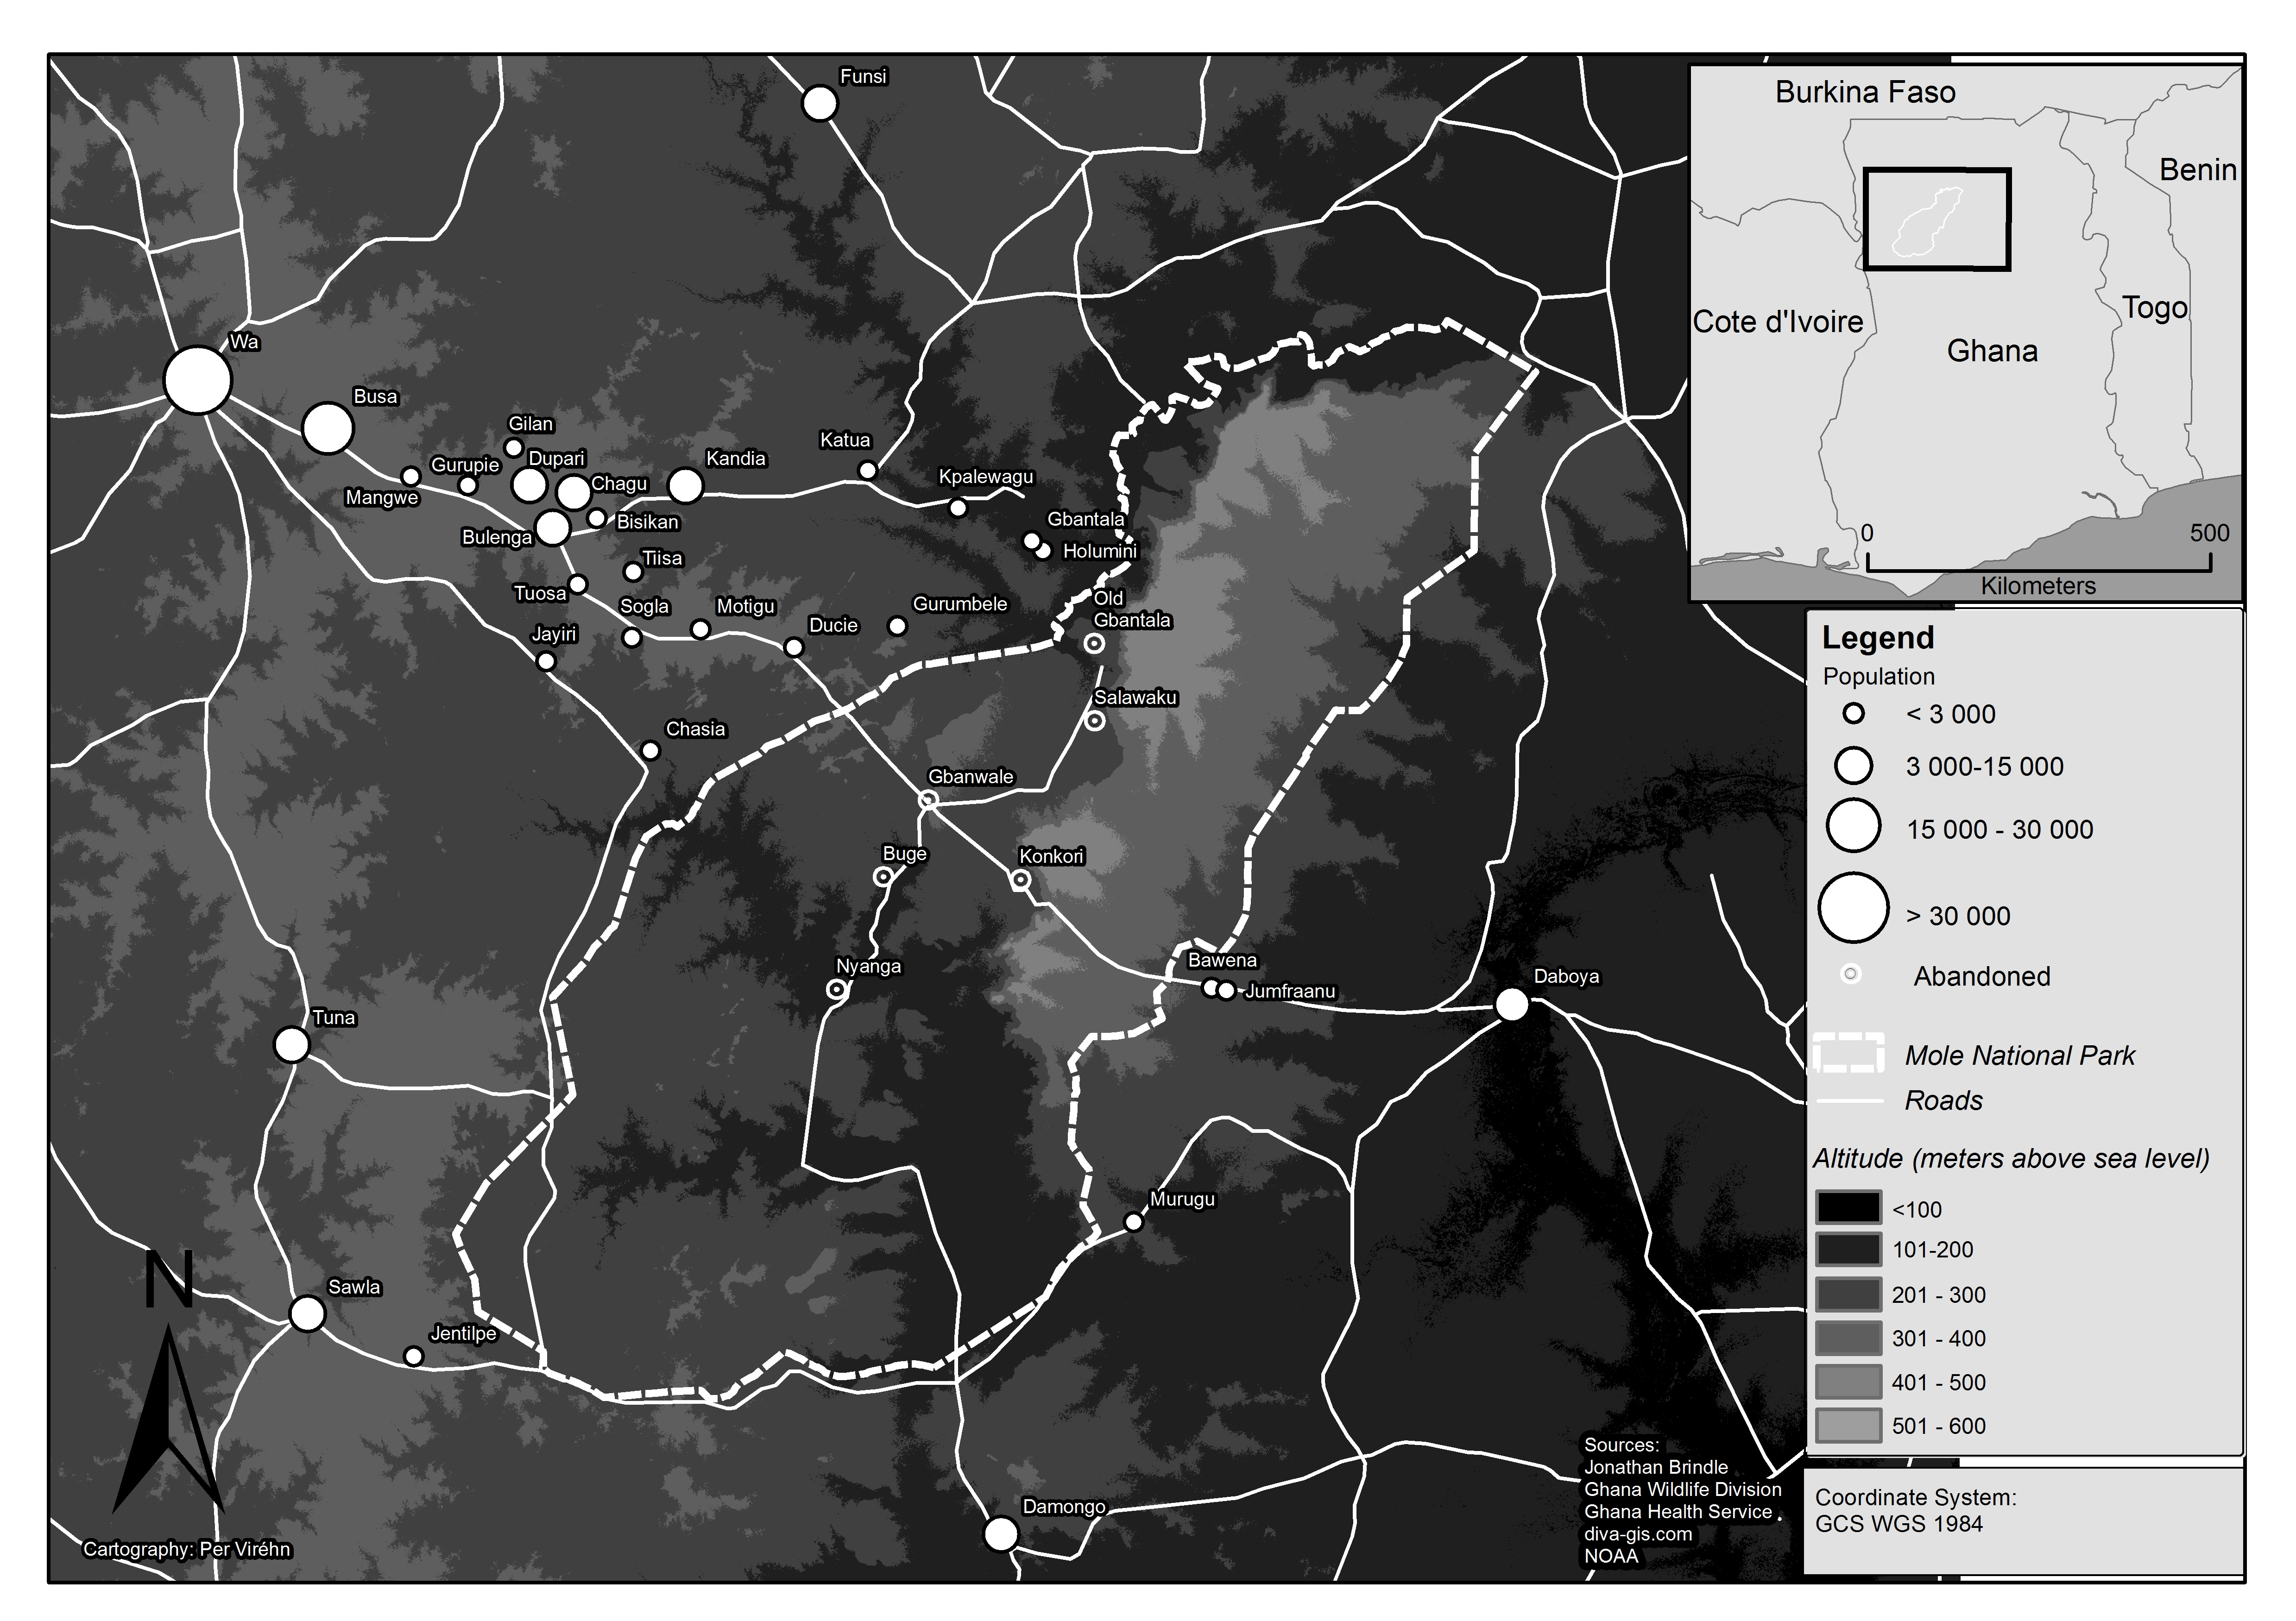
\includegraphics[height=4.8in]{Graphic/Maps/project-4.jpg}
% climap.pdf: 0x0 pixel, 0dpi, 0.00x0.00 cm, bb=

\caption[]{Caption\label{fig:}}
\end{sidewaysfigure}


 

 
It is crucial to keep in mind that these three concepts (i.e. land, 
ethnicity, and language) are interwoven.   For instance, according to 
\citet{Daan94},  {\it Chakali}  consists of  thirteen communities 
and 
their inhabitants:  Bulenga, Tiisa, Sogla, Tuosa, Chagu, Motigu, Ducie, Katua, 
Bisikan, Kandia, Dupari, Gilan and Gurumbele.  By contrast, the 
sociolinguistic 
censuses which I carried out indicate that {\it Chakali} is the 
language 
of the inhabitants and forefathers of  Tiisa, Sogla, Tuosa,  Motigu, Ducie, 
Katua, and  Gurumbele exclusively.


The \is{demonym}demonym for the people of these seven villages literally 
translate to  
{\it m̩̀ ŋmá kàà} {\it (lit.)}   `I say that',  whereas that of  the 
people 
of Bulenga and surrounding villages translate to   {\it ŋmɪ́nɪ́ŋ dʒɔ̀ŋ}  `What 
is it?'.   In this folk-sociolinguistic categorisation, the Waala are the {\it 
ǹ̩ jɛ́ jàà} `I say that'.\footnote{\citet[525]{Ratt32b} writes that the 
Awuna,  a Kasem dialect also known as Aculo \citep[147]{Nade89},  has earned 
its 
appellation based on a habit of  ``prefacing an observation with the words''  
{\it a wun a} `I say'. It is indeed the case that a Chakali  can open a sentence 
with {\it m̩̀ ŋmá kàà, ...}  `I say that, ...'. To hear the  Ghanaian 
English opening 
expression {\it à sé ɛ̃̀ɛ̃̀}  `I say eh, ...'   in Wa town is not 
unusual.}   Another popular distinction  is that of `black' and `white' 
Chakali;  respectively, the eastern block is the {\it tʃàkàlbúmmò} `Black 
Chakali',  a notion which connotes  secretive individuals, possessors of 
powerful medicine. I was told that Tuosa and Tissa are not part of the `Black 
Chakali'.   The western block is  the   {\it tʃàkàlpʊ̀mmá}  `White Chakali', 
i.e. people who are talkative and cannot hold back.\footnote{This comes from 
my 
`Black Chakali' consultants. Obviously, if one asks the same question in Bulenga 
and surrounding villages one may get a different interpretation of the 
distinction.}  This way of making a distinction 
between linguistic groups corresponds more or less to what \citet[2-3]{Good54} 
calls eastern Chakali and Western Chakali. Within the 
{\it m̩̀ ŋmá kàà}, there 
exist lexical, phonological, and prosodic variations which validate 
folk-dialectology. The lect of Katua, Tiisa and Tuosa,  on one hand, and the 
lect of Ducie and Gurumbele, on the other hand,  are considered the farthest 
apart on a continuum.\footnote{A Sogla-Motigu lect   could be situated somewhere 
in the middle of such continuum. One version of the migration and creation of 
Katua, Tiisa,  and Tuosa is presented in \citet[74-82]{Sali08}.} Examples 
of lectal variation are provided in \citet{brin15c}, but one recurrent 
illustration of folk-dialectology  is  how each village would express `to 
eat yam':   Motigu, Gurumbele, Tuosa, Tiisa,  and Katua  `chew' yam {\it 
(tie)}, 
whereas Ducie  `eat' yam {\it (di)}.  And while `yam' is pronounced {\it 
kpããŋ} in Motigu, Gurumbele,  and Ducie, it is pronounced {\it pɪɪ} in Tuosa, 
Tiisa,  and Katua. Thus, if someone says {\it tie kpããŋ}, he/she is 
easily identified as someone from either Gurumbele or Motigu.  The expression 
{\it di kpããŋ} is typically uttered by someone from  Ducie,  and {\it tie pɪɪ} 
by someone from Tuosa,  Tiisa, and Katua.  Still, each village is recognised to 
have a set of unique features. For instance, within the Ducie-Gurumbele lect, 
Ducie people consider that {\it Bɛ̀lɪ́lɪ́ɪ́}, the Gurumbele lect,  is a lect 
resembling a mixture of {\it Dùsélíí}, the lect of Ducie, and the lect 
of Gbanwale {\it (gbúŋwálɛ́)}, i.e. a variety of Tampulma. They also say that 
the Gurumbele lect is ``stretched'', and that the speakers ``pull their 
words''. The 
people of Gurumbele believe the opposite, saying that Ducie lect  is 
 ``short''.  These statements are  reported in (\ref{ex:SOC-bele-duc-lect}). 



\begin{exe}
 \ex\label{ex:SOC-bele-duc-lect}
\begin{xlist}
 \ex\label{ex:SOC-bele-lect}
\gll bɛ̀lɪ́lɛ́ɛ́ tàá tɪ̀ŋ ʊ̀ já tátʊ́ʊ̀\\
lect.type language {\art} {3\sg} {\sc hab} pull.{\foc}\\
\glt `The language of Gurumbele; it pulls/stretches.'

 \ex\label{ex:SOC-ducie-lect}
\gll dùsíéléé tàá tɪ̀ŋ ʊ̀ jáá bòrò rò\\
lect.type language {\art} {3\sg} {\ident}  short {\foc}\\
\glt `The language of Ducie; it is short.'
\end{xlist}
\end{exe}

Despite the above linguistic and anecdotal facts reporting the presence 
of variations,  all the Chakali lects are mutually intelligible.


\subsection{Language Vitality}
\label{sec:vital}

The number of Chakali speakers is close
to 3500 individuals. It is spoken by all community members in Gurumbele and 
Ducie, and by
the majority in Motigu and Katua. It is spoken to a lesser extent in Sogola,
Tuosa,  and Tiisa.  In the other villages which are considered as  parts of
Chakali land, people speak a language similar to Waali, the language of  Wa, or
Bulengi, the language of Bulenga. Waali is known by the majority of Chakali
speakers,  but is used differently from community to community.   Chakali is 
believed
to be on the road to extinction: some believe that Waali and Bulengi are the
languages which will be spoken throughout the whole of the Chakali villages in 
the
coming decades.



\begin{sidewaysfigure}
\footnotesize
  \centering
 \begin{tabular}{p{5cm}p{3.5cm}p{3.5cm}p{3.5cm}}


 %\begin{Atabular}{ll}
\toprule
    Factors & \multicolumn{3}{c}{Measures}\\[1ex]\midrule
 &E1&E2&E3\\[1ex]\midrule

1. Intergenerational language transmission &  {severely endangered} 
(2) & {unsafe} (4)& {safe} (5)\\

2.  Absolute number of speakers  &
\multicolumn{3}{c}{[{ 3484}]}\\ 

3. Proportion of speakers within the total population &
\multicolumn{3}{c}{[{severely
endangered}  (2) ]}\\

4.  Trends in existing language domains & {highly limited domains}
(2)& {dwindling domains} (3)&{multilingual parity} (4)\\

5.  Response to new domains and media& & [{
inactive-minimal}
(0-1)]& \\


6.  Materials for language education and literacy & 
\multicolumn{3}{c}{[{no orthography available} (0)]}\\

7. Governmental and institutional language attitudes
and policies, including official status and use &
\multicolumn{3}{c}{[{active
assimilation} (2) ]}\\


8. Community members attitudes toward their own language &-&-&{all
members value their language and wish to see it promoted} (5) 
\\

9.  Amount and quality of documentation &
\multicolumn{3}{c}{[{undocumented-inadequate} (0-1) ]}\\


\bottomrule
  \end{tabular}
  
\caption[Estimated degree of endangerment for the E1, E2 and E3 
villages]{Estimated degree of endangerment for the E1 \{Tuosa, Tiisa, Sogla\}, 
E2 \{Katua, Motigu\} and E3 \{Gurumbele, Ducie\}. A value within square brackets 
 applies to E1, E2 and E3 villages as a whole. The number in parentheses is a 
relative grade used in the  language vitality assessment  
\citep[see][7]{Reco03}} \label{tab:estimate-endangerment}

\end{sidewaysfigure}




 \citet{brin15c} determines the vitality of  Chakali using the 
questionnaire developed in 
\citet{Reco03} and  suggests a division of the Chakali
villages into three groups, which are presented in Figure 
\ref{tab:estimate-endangerment}. 
Sogla,
Tiisa,  and Tuosa correspond to the villages where the intergenerational
transmission is ineffective and where Waali is used in formal and informal
domains. They are the endangered-1  villages (E1).  Motigu and 
Katua correspond to 
E2
villages. In both villages,  Waali is encroaching on  Chakali in
formal and informal domains. The situation is not alarming since Chakali is
spoken by the majority and  the intergenerational transmission is effective, but
given the average population size of the villages and the recent conversion to
Islam of their youth, among other factors, it is worth considering that a 
language shift to Waali may
take place within a short period of time.  A. B. Sakara and H. S. Daanaa, both 
born in
Tuosa, told me that Chakali was spoken by everyone in their village when they
were children, i.e. in the 1950s and 1960s. There  are no signs indicating that 
the same 
language replacement which took place in Tuosa  cannot take place in Motigu and
Katua. Finally, the E3 villages, Gurumbele and Ducie, show the most effective 
intergenerational transmission of the Chakali language. Both villages also 
establish local alliances (i.e. marriage, common shrines, one assembly man for 
both villages, etc.). Waali is spoken and understood, yet it is usually spoken 
in specific  domains, for instance  in official visits from the district or 
regional capital conducted by governmental bodies,  and  to  Waali-speaking 
visitors, traders,  or migrant farmers.


\subsection{Data Collection Method}
\label{sec:lects}

Each year since 2007 I  made a field trip to the Wa East District of Ghana, 
usually in the dry season, i.e.  a  period between February and  May.  Most of 
my stays were spent in a Chakali-speaking village. I had several overnight stays 
in Motigu, Gurumbele,  and Wa, and a few day trips to Katua, Tiisa, Tuosa, and 
Sogla. The linguistic data was gathered mainly in Ducie, and sociolinguistic 
surveys were conducted in Katua, Motigu, Sogla, Ducie and Gurumbele.  

%a person correctly identified the ethnic group of my tutor b y the way I was 
%speaking



Different elicitation techniques were used to gather words and sentences.  The 
most authentic and
natural data comes from impressionistic auditory transcription of transactions 
at the market, meetings 
with the elders,  and interviews with commoners. In these cases wordlists were 
created out of the transcriptions. The least natural data are pieces of 
translation work  or exchanges of information with consultants of the type `how 
do you say X', where X stands for an intended entity or proposition, using 
English or Chakali as the medium of communication. Translations from English to 
Chakali and 
from Chakali to English  were performed through a  collaboration with 
 my main consultants, namely: 
Daniel Kanganu Karija (male, 58 Y.O., Ducie), Fuseini Mba Zien (male, 54 Y.O., 
Ducie), Awie Bakuri Ahmed (male, 31 Y.O., 
Gurumbele), and Afia Kala Tangu 
(female, 34 Y.O., Ducie). Quantitative studies required at times as many as 
50 different speakers, all of them from Ducie. The results of some of these 
studies are reported in  
\citet{Brin12, brin16}.

Another method of 
elicitation 
consisted of having a significant number of native speakers interpreting,
identifying and expressing perceived stimuli.  Stimulus-based data collection
has the advantage of being free from interference and provides the researcher
with a level of authenticity unattainable in (bilingual) elicitation of
paradigms
and wordlists.  Since the data collection was carried
out with several individuals, the degree of consensus within the responses can
be interpreted as signalling core, secondary, or `accidental'
meaning. The same method is useful in practical lexicography work
when the discovery procedure involved  taxonomies unknown to the researcher. For
instance, the domains of animals and plants required the identification of
species and their associated pronounciation. A problem arises when the visual
access to some species  is practically
impossible, e.g.   hyenas or seasonal plants. While working on  the 
lexical database, many species were identified using
illustrations. One disadvantage often encountered with this approach to lexicon
and
grammar discovery is that standard stimuli  face
the problem  of cross-cultural applicability.  In the context of  northern 
Ghana, unfamiliar items or scenes depicted may cause
disagreement in
the overall description, if not confusion.  
Another obstacle is that pictures and illustrations may lack 
elementary features, such as texture, odour, size, etc., 
which are crucial for
 the identification of a species.  For
instance,
since  only  illustrations and pictures found in \citet{Cans61, Trap06} were 
used,  arriving at a consensus when identifying  
species of snake has proved difficult.   Therefore,  I believe I used the most 
satisfactory data collection strategy in such research context. Needless to say 
every piece of Chakali data in this book comes from my own transcription of 
speech. 
 
 
 


\section{User's Guide}
\label{sec:cont-descr}

At a macrostructure level, the Chakali-English dictionary is followed by the 
English-Chakali reversal index.  They contain information extracted  from a  
lexical database which I started   in 2007 using the software {\it Field 
Linguist’s Toolbox}  and imported in {\it Language Explorer (FLEx)} in  2012.  
The entries appearing in the dictionary are made out of  only a selection of  
the lexicographic fields and values available in the lexical database.

The passage from unwritten to written has the inevitable consequence of 
favouring a dialect. Any native speaker of Chakali would easily identify that 
Ducie was the community where the majority of the data was collected.  
Corresponding expressions from other varieties of Chakali are present, when they 
exist,  but more work is definitely needed.   Addressing the issue of convention 
and standardisation will require a  group of devoted contributors from distinct 
communities. There is no reason to treat the decisions taken in this book, 
especially regarding the orthography,  as the standard. It is advised to keep in 
mind that orthographic consistencies  and English translations and definitions 
are always challenging. 


% % It is valuable to identify lectal and generational variations, such as,
% % expressions used in one village but not in another and obsolete
% % expressions representative of the oldest generation. Other deficiencies 
% % in the 
% % current version are the
% % inadequate description of forms and functions in the verbal domain, of which
% % prosody is crucial in determining aspectual distinctions. 



\subsection{Chakali-English Dictionary}
\label{sec:cli-eng-entry}



The Chakali-English dictionary consists of over 3200 Chakali 
\is{headword}headword 
entries (a.k.a. \is{lemma}lemmas).
The transcription employs the 
orthography described in Chapter \ref{sec:chap-phono}.  It uses a Latin 
alphabet 
supplemented 
with symbols from the International 
Phonetic Alphabet (IPA), so the spelling-sound correspondence is direct.  A 
full list of the 
orthography symbols used in the dictionary and some guidance to their 
pronunciations are displayed in Table \ref{tab:orth-symb}.

\begin{table}[h]
  \caption{Orthography and other symbols\label{tab:orth-symb}}
\small
 \begin{tabular}{llll}
p & voiceless bilabial plosive & w&labio-velar approximant\\
b & voice bilabial plosive &j & palatal approximant \\
t & voiceless alveolar plosive &r & alveolar trill/flap\\
d &  voiced alveolar plosive&o& close-mid back rounded\\
k & voiceless velar plosive  &ɔ& open-mid back rounded\\
g & voiced velar plosive &e& close-mid front unrounded\\
ʔ & glottal stop &ɛ& open mid front unrounded\\
kp & voiceless labio-velar plosive &u& close back rounded\\
gb & voiced labio-velar plosive&ʊ& near close near back rounded\\
f & voiceless labio-dental fricative &i& close front unrounded\\
v & voiced labio-dental fricative  &ɪ& near close near front unrounded\\
s & voiceless alveolar fricative &a& open front unrounded\\
z & voiced alveolar fricative &ə& mid central\\
ɣ & voiced velar fricative&$[$ $]$ & phonetic representation\\
h & voiceless glottal fricative & ː & emphasis over or long segment\\
tʃ & voiceless postalveolar affricate & V̆ & extra short vowel\\
dʒ & voiced postalveolar affricate&C̩& syllabic consonant\\
m & bilabial nasal &  Ṽ & nasalized   vowel\\
n & alveolar nasal& V̀ & low tone \\
ɲ & palatal nasal &  V̄ & high tone \\
ŋ & velar nasal& V́ & high tone \\
ŋm & velar-labial nasal&V̏  & extra-low tone \\
l & alveolar lateral approximant  & &\\
\end{tabular}

 \end{table}
 
 

For users accustomed to the literacy work of GILLBT\footnote{Reference is made
to the literacy work on Vagla,  Tampulma, and Pasaale  of Marjorie 
Crouch\dag, Patricia Herbert, Noah Ampen, Kofi
Mensah,
Mike Toupin, Vicky Toupin, Ian Gray,  and Claire Gray.} the correspondences
in Table \ref{tab:corr-our} identify the differences between their 
transcriptions and mine. The
transcription adopted in this dictionary  appears to the right side of the 
arrows. 


\begin{table}[h]
\caption[]{Correspondences of orthographies\label{tab:corr-our}}
 \begin{center}
\framebox[3in]{
\begin{tabular}{lllllll}
% ng &$\leftarrow$& ŋ  & \hspace*{5ex} y&$\leftarrow$& j\\
ny &$\leftarrow$& ɲ  &\hspace*{5ex} Vh&$\leftarrow$&  Ṽ \\
ch  &$\leftarrow$& tʃ  &\hspace*{5ex}  i&$\leftarrow$&ɪ, i\\
j &$\leftarrow$&dʒ  &\hspace*{5ex}  u&$\leftarrow$& ʊ, u \\
y &$\leftarrow$&j  &\hspace*{5ex}  &&
\end{tabular}  
}
\end{center}
\end{table}



The headwords  are structured alphabetically  although an arbitrary decision was 
taken to place the letter `{\it  dʒ}' after `{\it  d}', `{\it  gb}' after `{\it  
g}', 
`{\it  kp}' after `{\it  k}',  `{\it  ɲ}'  and `{\it  ŋm}' successively after 
`{\it  n}',  
and `{\it  tʃ}' after `{\it  t}'.  All headwords are equal and appear at the 
left 
side of the column. Three representative entries of the Chakali-English 
dictionary are presented in Table \ref{tab:illu-dict}.\footnote{The circled 
numbers are there for reference purposes only.}

\begin{table}[h]
\caption[]{Illustrations of the Chakali-English dictionary 
entry\label{tab:illu-dict}}
 \begin{center}
\framebox[4in]{
\begin{tabular}{p{9cm}}
% \Circled{1}{\it  fi} \Circled{2}[fí]  \Circled{3}{\itshape num}.
\Circled{5}ten \\[1ex]

\Circled{1}{\it   bʊzaal}  \Circled{2} [bʊ́záàl] \Circled{8}cf: 
bɪɪzimii. \Circled{3}n.   \Circled{5} Stone partridge, type of bird  
\Circled{9}{\it 
Ptilopachus 
petrosus}   \Circledd{10} Pl: bʊzaalɛɛ \\[1ex]

\Circled{1}{\it   kpa}  \Circled{2}[kpà] 
\Circled{8}cf: paa; cf: jʊʊ$_{1}$. \Circled{3}v  \Circled{4}1) \Circled{5} take 
 
\Circled{6}kpá à pár tɪ̄ɛ̄ŋ. \Circled{7}Give me the hoe.  
\Circled{4}2) \Circled{5} to marry a woman \Circled{6}  ʊ̀ kpáʊ́ rà.  
\Circled{7}He married her

\end{tabular}
}
\end{center}
\end{table}


An entry starts with a  headword (\Circled{1}), which is immediately followed by 
its phonetic representation (\Circled{2}). This representation adds tones and 
other information on the pronunciation. Words which do not bear tones in the 
phonetic representation field are considered as either toneless or  unresolved. 
The grammatical category (\Circled{3}) provides  the word class of the headword. 
Open class items, i.e. nouns and verbs,  are the most frequent. A plural form  
is provided for the majority of the nouns \Circledd{10}. Cross references  
(\Circled{8}) appear before the part-of-speech and after the phonetic form. A 
type of variations to which different spellings or form have to be assigned is 
placed after the phonetic form. 


The meaning  is represented in the following way: if the headword has only one 
sense,  the part of speech immediately precedes the English definition 
(\Circled{5}).  If the headword has more than one sense,  a number followed by a 
right parenthesis (\Circled{4}) enumerates the different senses. When Chakali is 
translated into English using many expressions, these are separated by a comma. 
If a word typically collocates with a concept, this is expressed within  
parentheses in the English translation.  An example of usage (\Circled{6}) 
precedes its English translation (\Circled{7}). If literal and/or not easily 
translatable, this translation contains a parenthesis with clarification.

\subsubsection{Prosody}
\label{sec:INT-prosody}

The examples are all marked with diacritics which represent the prosody as I 
perceived it during the transcription work. A  short description of tone and 
intonation is provided in Section \ref{sec:tone-intonation}. At this stage, the 
transcription and description of tone will require an analysis of considerable 
sophistication, something which deserves a separate study. The convention for 
marking tone is:  high (  ́), low (  ̀), mid   (  ̄),  and super-low ( ̏ ).  
There are several issues linked to doing the transcription by ear and lacking a 
convention. For instance, due to the general downdrift,  the prosody on 
single words are easier to represent with the diacritics compared to longer 
expressions.

\subsubsection{Scientific name}
\label{sec:INT-sci-name}

To  add the referential stability needed for future comparison between
traditional  and scientific  taxonomies, scientific names appear in italics  
(\Circled{9}).   References to scientific
names of  plants and trees were taken from 
\citet{hawt06},  of  snakes from \citet{Cans61}  and \citet{Trap06}, and of  
birds 
from \citet{borr02}.




\subsubsection{Grammatical category}
\label{sec:INT-other-lex-field}

The grammatical categories (a.k.a  word classes or parts of speech)  used in the 
dictionary are all described in Section \ref{sec:gramsketch}. They are 
distinguished using distributional and inflectional criteria. Table 
\ref{tab:dict-abb} offers a  list of the sections in the grammar outline where 
each grammatical  category can be found, together with their dictionary 
abbreviation.


% \begin{table}[h]
%  \caption{Grammatical Categories and Sections\label{tab:}}
%   \centering
%   \begin{tabular}{llll}
% \lsptoprule 
% Grammatical Category & Abbreviation & Section \\
% article & 
% noun & {\itshape n} &  \\
% 
% 
%  \\
% \midrule
% 
%     
% \lspbottomrule
%   \end{tabular}
% \end{table}

% 
% verb ({\itshape v}),% 
% qualifiers ({\itshape qual}) 
% and quantifers  ({\itshape quant}), which modify 
%  nouns in  noun phrases,  adverbs  ({\itshape adv}) , which modify  verb phrases
%  or  clauses,  articles ({\itshape art}), which combine with a noun to indicate
%  the type of reference being made, classifier  ({\itshape clf}), which
%  is a selectional prefixed onto property denoting expressions and classify the
% referent either as human, concrete-(non)aninmate or abstract, relational noun
% ({\itshape reln}), which designates
% a locative search domain of an object,
% postposition ({\itshape postp}),  which signals that the
% constituent in which they appear is locative, ...
% 
% ,connective
% ,complementizer
% ,complex verb
% ,demonstrative
% ,focus
% ,ideophones
% ,interrogative
% ,interjection
% ,imperative
% ,iteratif
% ,negation
% ,numeral
% ,onomatopea
% ,postposition
% ,reciprocal
% ,reflexive
% ,tam
%


\subsubsection{Loans and their etymology}
\label{sec:INT-loan-ety}


Loan words are given a source and when necessary the source's pronunciation and 
gloss. Some are well-established, and others are intuitive. As the sources are 
not 
always easy to identify, some are followed by a question mark. I  put the 
word  {\it ultimately} (abbreviated {\it ultm.}) prior to the source language
to mean that the loan word might not have been borrowed directly from the 
speakers of the language with which the word is associated. For example, it is 
most likely that all English words entered Chakali  through contact with 
speakers of other Ghanaian languages.  Section \ref{sec:GRM-borr-noun} offers an 
overview of languages from which Chakali may have borrow.  References to 
etymologies are mainly taken from \citet{newm07hausa}, \citet{daku07},  
\citet{daku09ga},  \cite{vagl80},  and  \citet{Dume11}.


\subsection{English-Chakali Reversal Index}
\label{sec:eng-cli-entry}

The English-Chakali reversal index is a list of  alphabetically organized 
English headwords (\Circled{1}). As shown in Table 
\ref{tab:illu-index}  the headword may be 
associated with  more than one  Chakali 
gloss entry (\Circled{5}).  



\begin{table}[h]
\caption[]{Illustration of the English-Chakali reversal 
index entry\label{tab:illu-index}}
\begin{center} 
\framebox[3in]{

\begin{tabular}{lll}
 \Circled{1}grasshopper (type of) & \Circled{3}{\itshape n.} & 
\Circled{5}{hɔ̃ʊ̃} \\
 & \Circled{3}{\itshape n.} & \Circled{5}{tʃɛlɪntʃɪɛ} \\
 & \Circled{3}{\itshape n.} & \Circled{5}{kɔkɔlɪkɔ} \\
\end{tabular} 
}
\end{center} 
\end{table}



English  headwords are reduced to 
minimal terms in order to have the index easily searchable. 
Several English expressions can be associated with one Chakali word: for 
instance, 
all Chakali tree names get {\it tree (type of)} but only some have known 
English expressions associated to  them, e.g. {\it Shea tree}. Each Chakali 
word is preceded by its
word class (\Circled{3}). 


\subsubsection{Dictionary Abbreviations}
\label{LEX:abbrev}

The list of abbreviations used in the dictionary is provided in Table 
\ref{tab:dict-abb}, together with their meaning as well as  the section of the 
grammar that covers the related topics. 

% It contains some notions which are
%  self-explanatory. Others can be found in Section \ref{}. 

\begin{table}[h] 
\footnotesize
  \centering
 \caption{Dictionary Abbreviations}
  \label{tab:dict-abb}
% 
 \begin{tabular}{lll}
art   &    article   & \ref{sec:GRM-np-def-articles}\\
clf   &    classifier   &\ref{sec:classifier}\\  
comp   &   complementizer   &\ref{GRM-clause-subord}\\  
conn   &    connective   &\ref{GRM-clause-coord}\\   
cpx    &    complex   &\ref{sec:GRM-complex-verb}\\   
dem   &   demontrative   &\ref{sec:GRM-demons}\\
enum   &    enumerative usage &\ref{sec:NUM-enum}\\
etym   &    etymology &\ref{sec:GRM-borr-noun}\\
foc    &    focus   &\ref{sec:GRM-foc-neg}, \ref{sec:GRM-focus}\\    
  from    &    borrowed word &\ref{sec:GRM-borr-noun}\\
hum+/-   &   (non-)human   & \ref{sec:GRM-pronouns}, \ref{sec:GRM-gender}\\
ideo    &    ideophone   &\ref{sec:GRM-onoma}\\ 
ints    &    intensifier   &\ref{sec:GRM-intensifier}\\ 
interg   &    interrogative     &\ref{sec:GRM-interg-pro}\\
 interj    &    interjection   &\ref{sec:GRM-greet}\\  
   itr    &    iterative   & \ref{sec:GRM-preverb-iteration}\\
    Lit    &    literal meaning & \\
  n    &    noun   & \ref{sec:GRM-noun}\\
neg    &    negation   & \ref{sec:GRM-foc-neg}, \ref{sec:GRM-verb-neg}\\  
num   &   numeral  &  \ref{sec:GRM-numeral}\\
ono   &   onomatopoeia   & \ref{sec:GRM-onoma}\\
phr   &    phrase   &    \\
pl    &   plural   & \ref{sec:GRM-noun-classes}, \ref{sec:GRM-PluralVerb}, 
\ref{sec:GRM-personal-pronouns}\\
poss    &    possessive   &\ref{secːGRM-poss-pro}\\
postp   &   postposition  &\ref{sec:SPA-postp}\\
pro    &    pronoun &\ref{sec:GRM-pronouns}\\
propn   &   proper noun &\ref{sec:GRM-prop-noun}\\
pv    &    pre-verb particle &\ref{sec:GRM-precerv}\\
qual    &    qualifier &\ref{sec:GRM-qualifier}\\
quant   &   quantifier &\ref{sec:GRM-quantifier}\\
 reflex   &   reflexive   &\ref{sec:GRM-recipro-reflex}\\ 
rel.n   &    relational noun &\ref{sec:SPA-relnoun}\\
sc& scientific name & \\
see    &   cross-reference & \\
  sg   &   singular & \ref{sec:GRM-noun-classes}, \ref{sec:GRM-PluralVerb}, 
\ref{sec:GRM-personal-pronouns}\\
 st   &   strong pronoun &\ref{sec:GRM-personal-pronouns}\\
synt   &     taboo synonym &\ref{sec:GRM-ling-taboo}\\
 ultm    &    ultimately &\ref{sec:GRM-borr-noun}\\
usage   &    location of usage & \\
    v   &   verb &\ref{sec:GRM-verb-lexeme}\\
variant    &    variant form & \\
 wk   &   weak pronoun &\ref{sec:GRM-personal-pronouns}\\
   1, 2, 3  &    first, second, or third person 
&\ref{sec:GRM-personal-pronouns}\\

\end{tabular}

 \end{table}




\section{Grammatical Outlines}
\label{sec:intro-outline}

%Part \ref{}%2

Chapter  \ref{sec:chap-phono}   presents of a brief outline of the phonology. It 
is principally based on phonetic representations available in the dictionary.   
The phoneme inventory,  syllable structures and minimal pairs are identified. In 
addition, phonotactics and suprasegmentals are briefly discussed. The software 
{\it Dekereke} was used to investigate phonotactic generalizations and search 
for specific features and environments.\footnote{Thanks to its creator Rod 
Casali for his continual help.}  Based on the transcriptions of various 
narrative types and controlled elicitation, the grammar outline of Chapter 
\ref{sec:gramsketch} offers an overview of  the essential of word and sentence 
formations in the language, as well topics of linguistic usages of cultural 
relevance. The glossing tags in the abbreviations list are for the most part 
equivalent to the conventions designed in  \citet{Comr08b} and \citet{hasp14}.  
As a rule,   a three-line morpheme-by-morpheme  glossing for textual data is 
provided, but  four lines may exceptionally appear.  The first line is a 
representation of the object language, the second line consists of   tags 
representing  rough approximations  of the morpheme in the object   language 
(e.g. function, meaning,  and part-of-speech), whereas the third line is a free  
translation capturing the general meaning  conveyed in the object language's 
line. An additional line can appear when details are not evident in the gloss, 
or when another level of analysis is intended.  The use of capital letters in 
the  free translation corresponds to a focused constituent. The  non-overt 
expression of a feature is enclosed within round brackets following the   
Leipzig glossing rules. An interlinearized example  may  be accompanied by a 
reference  to a particular corpus text or  a situation in which the utterance 
was collected.


Some sections have  been published previously or appeared elsewhere. Section \ref{sec:GRM-numeral}  
is extracted and adapted from is a condensed   \citet{brin08b},  ...

Section \ref{sec:SPA-relnoun} in  \citet{Brin12},  ...
 
 
 \newpage
   

\newpage
\part{Chakali-English Dictionary}
 \ref{part:part1}

%%%%%%%%%%%%%%%%%%%%%%%%%%%%%%%%%%%%%%%%%%%%%%%%%%%%
%%%                                              %%%
%%%             Chapters                         %%%
%%%                                              %%%
%%%%%%%%%%%%%%%%%%%%%%%%%%%%%%%%%%%%%%%%%%%%%%%%%%%%


\newcommand{\headrulewidth}{0pt}
\setlength{\columnsep}{3em}
\setlength{\parindent}{0pt}

\renewcommand{\lsgloss}[1]{}
\begin{letter}{}
%------------------------------
\newentry
\homograph{1}%
\headword{a}%
\hypertarget{hvo10548}{}%
\ipa{à}%
\synpos{art}%
\hypertarget{hvo36742}{}%
\definition{the}%
\lsgloss{the}%
%------------------------------
\newentry
\homograph{2}%
\headword{a}%
\hypertarget{hvo19063}{}%
\ipa{à}%
\synpos{conn}%
\hypertarget{hvo33565}{}%
\definition{and}%
\lsgloss{and}%
%------------------------------
\newentry
\homograph{3}%
\headword{a}%
\hypertarget{hvo33687}{}%
\ipa{a}%
\typevar{\hyperlink{hvo28176}{aa}}%
\synpos{pro}%
\hypertarget{hvo12802}{}%
\definition{non-human third person plural pronoun}%
\lsgloss{they (hum-)}%
%------------------------------
\newentry
\hypertarget{hvo19082}{}%
\headword{a bɔnɪ̃ɛ̃ nɪ}%
\hypertarget{hvo21042}{}%
\ipa{à bɔ́nɪ̃́ɛ̃́ nɪ́}%
\synpos{adv.phr}%
\hypertarget{hvo24677}{}%
\definition{maybe, perhaps}%
\lsgloss{maybe}%
{\startexample}
\hypertarget{hvo31611}{}%
\vernacular{à bɔ́nɪ̃́ɛ̃́ nɪ́ dʊ́ɔ́ŋ káá wàʊ̄.}%
\hypertarget{hvo31611}{}%
\modvernacular{\-à bɔ́nɪ̃́ɛ̃́ nɪ́ dʊ́ɔ́ŋ káá wàʊ̄.}%
\hypertarget{hvo19117}{}%
\trs{Perhaps it is going to rain.}%
%------------------------------
\newentry
\hypertarget{hvo3501}{}%
\headword{a ɲuu nɪ}%
\hypertarget{hvo22040}{}%
\ipa{àɲúúnī}%
\literalmeaning{head-on}%
\typevar{\hyperlink{hvo19426}{ɲuunɪ}}%
\synpos{conn}%
\hypertarget{hvo12618}{}%
\definition{therefore}%
\lsgloss{therefore}%
{\startexample}
\hypertarget{hvo41309}{}%
\vernacular{ǹ̩ wà kṕagá sákɪ̀r, àɲúúnɪ̄ ǹ̩ dɪ̀ válà nààsá.}%
\hypertarget{hvo41309}{}%
\modvernacular{ǹ̩ wà kṕa\-gá sá\-kɪ̀r, àɲúúnɪ̄ ǹ̩ dɪ̀ vá\-là nàà\-sá.}%
\hypertarget{hvo28254}{}%
\trs{I do not have a bicycle, therefore I am walking.}%
%------------------------------
\newentry
\headword{aa}%
 \typevarof{\hyperlink{hvo28377}{a}}%
%------------------------------
\newentry
\hypertarget{hvo5618}{}%
\headword{ãã}%
\hypertarget{hvo175}{}%
\ipa{ʔã́ã́}%
\synpos{n}%
\hypertarget{hvo29836}{}%
\definition{bushbuck}%
\lsgloss{bushbuck}%
\sciname{Tragelaphus scriptus}%
\plural{ãã\-ta}%
%------------------------------
\newentry
\hypertarget{hvo10500}{}%
\headword{ããnɪ}%
\hypertarget{hvo28405}{}%
\ipa{ʔã̀ã̀nɪ̀}%
\synpos{v}%
\hypertarget{hvo20837}{}%
\definition{to suspect someone of telling a lie}%
\lsgloss{suspect}%
%------------------------------
\newentry
\hypertarget{hvo30404}{}%
\headword{ããnuuba}%
\hypertarget{hvo24320}{}%
\ipa{ʔã̀ã̀nùùbà}%
\typecf{\hyperlink{hvo23390}{nuui}}%
\synpos{n}%
\hypertarget{hvo10961}{}%
\definition{suffering}%
\lsgloss{suffering}%
%------------------------------
\newentry
\hypertarget{hvo12701}{}%
\headword{aarɪ}%
\hypertarget{hvo24782}{}%
\ipa{ʔáárɪ́}%
\synpos{v}%
\hypertarget{hvo24818}{}%
\definition{to harvest unriped food stuff}%
\lsgloss{harvest}%
{\startexample}
\hypertarget{hvo17470}{}%
\vernacular{hàmɔ́nà kàá ààrɪ̀ móngòsò rō.}%
\hypertarget{hvo17470}{}%
\modvernacular{hà\-mɔ́nà kàá àà\-rɪ̀ món\-gò\-sò rō.}%
\hypertarget{hvo25811}{}%
\trs{Children will pick the prematured mangoes.}%
%------------------------------
\newentry
\hypertarget{hvo30147}{}%
\headword{abɛ}%
\hypertarget{hvo37026}{}%
\ipa{ʔàbɛ́}%
\synpos{n}%
\hypertarget{hvo7924}{}%
\definition{palm nut tree}%
\lsgloss{nut (palm)}%
\plural{a\-bɛ\-sa}%
%------------------------------
\newentry
\hypertarget{hvo24597}{}%
\headword{abie}%
\hypertarget{hvo14399}{}%
\ipa{abie}%
\typecf{\hyperlink{hvo18002}{awie}}%
\synpos{nprop}%
\hypertarget{hvo23662}{}%
\definition{Awie (person's name)}%
\lsgloss{Awie}%
\usage{Ka}%
%------------------------------
\newentry
\hypertarget{hvo25742}{}%
\headword{abluu}%
\hypertarget{hvo9643}{}%
\ipa{ʔábə̆̀lùù}%
\synpos{n}%
\hypertarget{hvo736}{}%
\definition{blue}%
\lsgloss{blue}%
\etymology{}%
\etymologyform{blue}%
\etymologysrc{ultm. English}%
\plural{a\-bluu\-so}%
%------------------------------
\newentry
\headword{abubusa}%
 \typevarof{\hyperlink{hvo34765}{abusabusa}}%
%------------------------------
\newentry
\hypertarget{hvo34765}{}%
\headword{abusabusa}%
\hypertarget{hvo11834}{}%
\ipa{ʔàbùsàbùsà}%
\typevar{\hyperlink{hvo24503}{abubusa}}%
\synpos{ideo}%
\hypertarget{hvo29545}{}%
\definition{type of color}%
\lsgloss{color (type of)}%
%------------------------------
\newentry
\headword{adʒudʒumo}%
 \typevarof{\hyperlink{hvo32015}{adʒumodʒumo}}%
%------------------------------
\newentry
\hypertarget{hvo32015}{}%
\headword{adʒumodʒumo}%
\hypertarget{hvo2956}{}%
\ipa{ʔàdʒùmòdʒùmò}%
\typevar{\hyperlink{hvo30230}{adʒudʒumo}}%
\synpos{ideo}%
\hypertarget{hvo40701}{}%
\definition{type of color}%
\lsgloss{color (type of)}%
%------------------------------
\newentry
\headword{ahɔhɔla}%
 \typevarof{\hyperlink{hvo36112}{ahɔlahɔla}}%
%------------------------------
\newentry
\hypertarget{hvo36112}{}%
\headword{ahɔlahɔla}%
\hypertarget{hvo15956}{}%
\ipa{ʔàhɔ̀làhɔ̀là}%
\typevar{\hyperlink{hvo38962}{ahɔhɔla}}%
\synpos{ideo}%
\hypertarget{hvo16026}{}%
\definition{yellowish color}%
\lsgloss{color (type of)}%
%------------------------------
\newentry
\hypertarget{hvo28714}{}%
\headword{aɪ}%
\hypertarget{hvo33695}{}%
\ipa{ʔàɪ́}%
\synpos{interj}%
\hypertarget{hvo20881}{}%
\definition{no}%
\lsgloss{no}%
%------------------------------
\newentry
\hypertarget{hvo18010}{}%
\headword{aka}%
\hypertarget{hvo40243}{}%
\ipa{àká}%
\synpos{conn}%
\hypertarget{hvo19922}{}%
\definition{and, then}%
\lsgloss{then; and}%
{\startexample}
\hypertarget{hvo7478}{}%
\vernacular{wáá ɲʊ̃́ã́ nɪ́ɪ́ àká tɪ̄ɛ̄ŋ.}%
\hypertarget{hvo7478}{}%
\modvernacular{wáá ɲʊ̃́ã́ nɪ́ɪ́ à\-ká tɪ̄ɛ̄ŋ.}%
\hypertarget{hvo12519}{}%
\trs{He drank the water then gave some to me.}%
%------------------------------
\newentry
\hypertarget{hvo4051}{}%
\headword{akɔlakɔla}%
\hypertarget{hvo1538}{}%
\ipa{ʔàkɔ̀làkɔ̀là}%
\synpos{ideo}%
\hypertarget{hvo31322}{}%
\definition{type of color}%
\lsgloss{color (type of)}%
%------------------------------
\newentry
\headword{alakadee}%
\hypertarget{hvo4133}{}%
\ipa{ʔálákádéè}%
 \typevarof{\hyperlink{hvo28009}{kasiu}}%
%------------------------------
\newentry
\hypertarget{hvo24948}{}%
\headword{alamʊsa}%
\hypertarget{hvo4169}{}%
\ipa{ʔàlàmʊ̀sà}%
\synpos{n}%
\hypertarget{hvo22320}{}%
\definition{Thursday}%
\lsgloss{Thursday}%
\etymology{}%
\etymologyform{àlhàmîs}%
\etymologysrc{ultm. Arabic, via Hausa}%
%------------------------------
\newentry
\hypertarget{hvo31225}{}%
\headword{alarba}%
\hypertarget{hvo36428}{}%
\ipa{ʔàlàrbà}%
\synpos{n}%
\hypertarget{hvo15126}{}%
\definition{Wednesday}%
\lsgloss{Wednesday}%
\etymology{}%
\etymologyform{lā̀r̃àbā}%
\etymologysrc{ultm. Arabic, via Hausa}%
%------------------------------
\newentry
\hypertarget{hvo16735}{}%
\headword{albasa}%
\hypertarget{hvo7913}{}%
\ipa{ʔálằbásà}%
\synpos{n}%
\hypertarget{hvo19653}{}%
\definition{onion}%
\lsgloss{onion}%
\etymology{}%
\etymologyform{àlbasā̀}%
\etymologysrc{ultm. Arabic, via Hausa}%
\plural{a\-le\-ba\-sa\-sa}%
%------------------------------
\newentry
\hypertarget{hvo31621}{}%
\headword{alɛɛfʊ}%
\hypertarget{hvo39187}{}%
\ipa{ʔálɛ́ɛ̀fʊ́}%
\synpos{n}%
\hypertarget{hvo35264}{}%
\definition{leaf used as soup ingredient to improve taste, known as vegetable amaranths}%
\lsgloss{amaranths (vegetable)}%
\sciname{Amarantus Debius}%
\etymology{}%
\etymologyform{àlayyàhō}%
\etymologygloss{spinach}%
\etymologysrc{ultm. Hausa}%
\plural{a\-lɛɛ\-fʊ}%
%------------------------------
\newentry
\hypertarget{hvo4679}{}%
\headword{alɪbaraka}%
\hypertarget{hvo22182}{}%
\ipa{ʔàlɪ̆̀bárákà}%
\synpos{n}%
\hypertarget{hvo2547}{}%
\definition{reduce price}%
\lsgloss{reduce price}%
\etymology{}%
\etymologysrc{ultm. Arabic, via Hausa}%
%------------------------------
\newentry
\hypertarget{hvo40806}{}%
\headword{alɪɛ}%
\hypertarget{hvo27480}{}%
\ipa{álɪ̀ɛ̀}%
\synpos{num}%
\hypertarget{hvo8237}{}%
\definition{two}%
\lsgloss{two}%
\typeEnum{\hyperlink{hvo34402}{ɲɛwã}}%
%------------------------------
\newentry
\hypertarget{hvo6501}{}%
\headword{alɪhaadi}%
\hypertarget{hvo40524}{}%
\ipa{ʔàlɪ̀háádì}%
\synpos{n}%
\hypertarget{hvo18511}{}%
\definition{Sunday}%
\lsgloss{Sunday}%
\etymology{}%
\etymologyform{lahàdì}%
\etymologysrc{ultm. Arabic, via Hausa}%
%------------------------------
\newentry
\hypertarget{hvo8371}{}%
\headword{aloro}%
\hypertarget{hvo10464}{}%
\ipa{álòrò}%
\synpos{num}%
\hypertarget{hvo27841}{}%
\definition{six}%
\lsgloss{six}%
\typeEnum{\hyperlink{hvo40788}{loroo}}%
\plural{a\-lo\-ro\-so}%
%------------------------------
\newentry
\hypertarget{hvo40008}{}%
\headword{alʊpɛ}%
\hypertarget{hvo20042}{}%
\ipa{álʊ̀pɛ̀}%
\synpos{num}%
\hypertarget{hvo14893}{}%
\definition{seven}%
\lsgloss{seven}%
\typeEnum{\hyperlink{hvo35316}{lʊpɛɛ}}%
%------------------------------
\newentry
\hypertarget{hvo17280}{}%
\headword{ame}%
\hypertarget{hvo21976}{}%
\ipa{ʔàmé}%
\synpos{interj}%
\hypertarget{hvo23758}{}%
\definition{so be it}%
\lsgloss{so be it}%
{\startexample}
\hypertarget{hvo38787}{}%
\vernacular{A: kúòsō tɪ́ɛ́ já tʃɪ́á. B: àmé.}%
\hypertarget{hvo38787}{}%
\modvernacular{A: kúò\-sō tɪ́ɛ́ já tʃɪ́á. B: à\-mé.}%
\hypertarget{hvo11982}{}%
\trs{A: Let God gives us tomorrow B: So be it.}%
\etymology{}%
\etymologygloss{amen}%
\etymologysrc{ultm. Hebrew}%
%------------------------------
\newentry
\headword{amiõ}%
 \typevarof{\hyperlink{hvo32049}{dʒɛbalaŋ}}%
%------------------------------
\newentry
\hypertarget{hvo17335}{}%
\headword{amɪ̃ɛ̃}%
\hypertarget{hvo24285}{}%
\ipa{àmɪ̃̀ɛ̃̀}%
\synpos{adv}%
\hypertarget{hvo12604}{}%
\definition{if so}%
\lsgloss{if so}%
%------------------------------
\newentry
\hypertarget{hvo10953}{}%
\headword{ammani}%
\hypertarget{hvo41168}{}%
\ipa{ʔámmànī}%
\synpos{n}%
\hypertarget{hvo10073}{}%
\definition{small dried fish}%
\lsgloss{small dried fish}%
\etymology{}%
\etymologyform{ámànī}%
\etymologysrc{Akan}%
\plural{ammani\-se}%
%------------------------------
\newentry
\hypertarget{hvo38768}{}%
\headword{amuŋ}%
\hypertarget{hvo14090}{}%
\ipa{àmùŋ}%
\typecf{\hyperlink{hvo38493}{bamuŋ}}%
\synpos{quant}%
\hypertarget{hvo33689}{}%
\definition{all (hum-)}%
\lsgloss{all (hum-)}%
%------------------------------
\newentry
\hypertarget{hvo16416}{}%
\headword{amʊnʊ}%
\hypertarget{hvo494}{}%
\ipa{ʔàmʊ́nʊ́}%
\typecf{\hyperlink{hvo24892}{badaarɛ}}%
\synpos{n}%
\hypertarget{hvo34021}{}%
\definition{type of wild cat}%
\lsgloss{wild cat (type of)}%
\etymology{}%
\etymologysrc{Tampulma}%
\plural{a\-mʊnʊsa}%
%------------------------------
\newentry
\headword{ana}%
 \typevarof{\hyperlink{hvo16622}{aŋ}}%
%------------------------------
\newentry
\hypertarget{hvo7828}{}%
\headword{anaasɛ}%
\hypertarget{hvo38728}{}%
\ipa{ánáásɛ̀}%
\typevar{\hyperlink{hvo33494}{naasɪ}}%
\synpos{num}%
\hypertarget{hvo29883}{}%
\definition{four}%
\lsgloss{four}%
\typeEnum{\hyperlink{hvo5343}{naasɛ}}%
%------------------------------
\newentry
\hypertarget{hvo35162}{}%
\headword{andɪakaaɲããwɪɛ}%
{\fixpron} %% []
\synpos{n}%
\lsgloss{cat}%
\typeSynT{\hyperlink{hvo15681}{diebie}}%
%------------------------------
\newentry
\hypertarget{hvo20906}{}%
\headword{andʒelindʒe}%
\hypertarget{hvo21118}{}%
\ipa{ʔàndʒèlìndʒé}%
\synpos{nprop}%
\hypertarget{hvo29248}{}%
\definition{eighth month}%
\lsgloss{eighth month}%
\etymology{}%
\etymologysrc{Waali}%
%------------------------------
\newentry
\hypertarget{hvo23987}{}%
\headword{angum}%
\hypertarget{hvo39712}{}%
\ipa{ʔángùm}%
\synpos{ono}%
\hypertarget{hvo38755}{}%
\definition{monkey's scream}%
\lsgloss{monkey's scream}%
{\startexample}
\hypertarget{hvo758}{}%
\vernacular{àwɪ́ɛ́ gbɪ̃̀ã̀ jáà wīī ángùm, ángùm, ángùm.}%
\hypertarget{hvo758}{}%
\modvernacular{à\-wɪ́ɛ́ gbɪ̃̀ã̀ jáà wīī án\-gùm, án\-gùm, án\-gù\-m.}%
\hypertarget{hvo17561}{}%
\trs{That is why the monkey sounds like angum, angum, angum.}%
%------------------------------
\newentry
\hypertarget{hvo36399}{}%
\headword{anĩĩ}%
\hypertarget{hvo27533}{}%
\ipa{ʔánĩ́ĩ́}%
\synpos{n}%
\hypertarget{hvo17684}{}%
\definition{Ebony tree}%
\lsgloss{Ebony tree}%
\sciname{Diospyros mespiliformis}%
\plural{\-anĩã}%
%------------------------------
\newentry
\hypertarget{hvo32628}{}%
\headword{anɪ}%
\hypertarget{hvo16371}{}%
\ipa{ànɪ́}%
\pos{conn}%
\typevar{\hyperlink{hvo6729}{nɪ1}}%
\sensenr{1}%
\hypertarget{hvo23444}{}%
\definition{and}%
\lsgloss{and}%
{\startexample}
\exnr{1}%
\hypertarget{hvo19258}{}%
\vernacular{ǹ̩ nɪ́ ǹ̩ tʃɛ́ná kàá kààlɪ̀ Wàà rā.}%
\hypertarget{hvo19258}{}%
\modvernacular{ǹ̩ nɪ́ ǹ̩ tʃɛ́ná kàá kàà\-lɪ̀ Wàà rā.}%
\hypertarget{hvo13641}{}%
\trs{Me and my friend will go to Wa.}%
\exnr{2}%
\hypertarget{hvo13817}{}%
\vernacular{ǹ̩ jáá bɪ̀nsá màtʃēō ànɪ́ fī.}%
\hypertarget{hvo13817}{}%
\modvernacular{ǹ̩ jáá bɪ̀n\-sá màtʃēō ànɪ́ fī.}%
\hypertarget{hvo30413}{}%
\trs{I am thirty years old.}%
\sensenr{2}%
\hypertarget{hvo34841}{}%
\definition{with}%
\lsgloss{with}%
{\startexample}
\hypertarget{hvo22587}{}%
\vernacular{ŋ̩̀ ŋmɛ́ná dáá rá ànɪ́ kàrántɪ̄ɛ̄ nɪ̄.}%
\hypertarget{hvo22587}{}%
\modvernacular{ŋ̩̀ ŋmɛ́ná dáá rá ànɪ́ kà\-rán\-tɪ̄ɛ̄ nɪ̄.}%
\hypertarget{hvo2945}{}%
\trs{I cut a tree with a cutlass.}%
%------------------------------
\newentry
\hypertarget{hvo20260}{}%
\headword{anɪ a muŋ}%
\hypertarget{hvo12189}{}%
\ipa{ànɪ́ ā mùŋ}%
\synpos{adv}%
\hypertarget{hvo31718}{}%
\definition{in spite of, even though}%
\lsgloss{in spite of}%
{\startexample}
\hypertarget{hvo3884}{}%
\vernacular{ʊ̀ wááwáʊ́ ànɪ́ à mùŋ dɪ́ ʊ̀ʊ̀ wɪ́ɪ́ʊ̄.}%
\hypertarget{hvo3884}{}%
\modvernacular{ʊ̀ wáá\-wáʊ́ ànɪ́ à mùŋ dɪ́ ʊ̀ʊ̀ wɪ́ɪ́ʊ̄.}%
\hypertarget{hvo8667}{}%
\trs{He came in spite of his illness.}%
%------------------------------
\newentry
\hypertarget{hvo8748}{}%
\headword{annulie}%
\hypertarget{hvo14138}{}%
\ipa{ʔánnúlìè}%
\typedialvarGu{\hyperlink{hvo7204}{nããnuule}}%
\synpos{n}%
\hypertarget{hvo6385}{}%
\definition{dragonfly}%
\lsgloss{dragonfly}%
\sciname{Epiprocta Anisoptera}%
\plural{annu\-le\-se}%
%------------------------------
\newentry
\hypertarget{hvo12456}{}%
\headword{ansa}%
\hypertarget{hvo32250}{}%
\ipa{ʔánsà}%
\pos{interj}%
\sensenr{1}%
\hypertarget{hvo4790}{}%
\definition{welcome}%
\lsgloss{welcome}%
\sensenr{2}%
\hypertarget{hvo18471}{}%
\definition{thanks}%
\lsgloss{thanks}%
%------------------------------
\newentry
\hypertarget{hvo17321}{}%
\headword{aɲãã}%
\hypertarget{hvo68}{}%
\ipa{ʔàɲã̀ã́}%
\synpos{n}%
\hypertarget{hvo39171}{}%
\definition{type of snake}%
\lsgloss{snake (type of)}%
\plural{\-aɲããna}%
%------------------------------
\newentry
\hypertarget{hvo12656}{}%
\headword{aɲɔ̃}%
\hypertarget{hvo11460}{}%
\ipa{áɲɔ̃̀}%
\synpos{num}%
\hypertarget{hvo13696}{}%
\definition{five}%
\lsgloss{five}%
\typeEnum{\hyperlink{hvo24096}{ɲɔ̃ɔ̃}}%
%------------------------------
\newentry
\headword{aŋmɛna}%
 \typevarof{\hyperlink{hvo19261}{ŋmɛna}}%
%------------------------------
\newentry
\hypertarget{hvo32478}{}%
\headword{aŋmunaŋmuna}%
\hypertarget{hvo25593}{}%
\ipa{ʔàŋmùnàŋmùnà}%
\synpos{ideo}%
\hypertarget{hvo1872}{}%
\definition{type of color}%
\lsgloss{color (type of)}%
%------------------------------
\newentry
\hypertarget{hvo16622}{}%
\headword{aŋ}%
\hypertarget{hvo6432}{}%
\ipa{ʔàŋ́}%
\typevar{\hyperlink{hvo27017}{ana}}%
\synpos{interrog}%
\hypertarget{hvo38679}{}%
\definition{who}%
\lsgloss{who}%
{\startexample}
\hypertarget{hvo12754}{}%
\vernacular{àŋ́ ɪ̀ɪ̀ kà nà à tɔ́ʊ̄ nɪ̄.}%
\hypertarget{hvo12754}{}%
\modvernacular{à\-ŋ́ ɪ̀ɪ̀ kà nà à tɔ́ʊ̄ nɪ̄.}%
\hypertarget{hvo31685}{}%
\trs{Who did you see at the village?}%
%------------------------------
\newentry
\hypertarget{hvo3375}{}%
\headword{aŋbuluŋ}%
\hypertarget{hvo25802}{}%
\ipa{ʔámbúlùŋ}%
\synpos{n}%
\hypertarget{hvo11598}{}%
\definition{Black berry, type of tree}%
\lsgloss{Black berry; tree (type of)}%
\sciname{Vitex doniana}%
\plural{aŋbu\-lu\-ŋso}%
%------------------------------
\newentry
\hypertarget{hvo26165}{}%
\headword{aŋkɪtɪ}%
\hypertarget{hvo15212}{}%
\ipa{ʔáŋkɪ́tɪ̀}%
\synpos{n}%
\hypertarget{hvo28169}{}%
\definition{handkerchief, thin fabric intended for personal hygiene, such as wiping one's hands or face}%
\lsgloss{handkerchief}%
\etymology{}%
\etymologysrc{ultm. English}%
\plural{a\-ŋkɪtɪsa}%
%------------------------------
\newentry
\hypertarget{hvo9687}{}%
\headword{aŋkʊrɔ}%
\hypertarget{hvo2981}{}%
\ipa{áŋkʊ̀rɔ̄}%
\synpos{n}%
\hypertarget{hvo4507}{}%
\definition{barrel, cask, drum container }%
\lsgloss{barrel}%
\etymology{}%
\etymologyform{anker}%
\etymologysrc{ultm. English, via Akan}%
%------------------------------
\newentry
\hypertarget{hvo6209}{}%
\headword{arɪdʒana}%
\hypertarget{hvo24915}{}%
\ipa{ʔàrɪ̆̀dʒánà}%
\typecf{\hyperlink{hvo14808}{lɛl}}%
\synpos{n}%
\hypertarget{hvo41090}{}%
\definition{heaven}%
\lsgloss{heaven}%
%------------------------------
\newentry
\hypertarget{hvo7333}{}%
\headword{arɪdʒima}%
\hypertarget{hvo24902}{}%
\ipa{ʔàrɪ̀dʒímà}%
\synpos{n}%
\hypertarget{hvo30686}{}%
\definition{Friday}%
\lsgloss{Friday}%
\etymology{}%
\etymologyform{jummàā̀}%
\etymologysrc{ultm. Arabic, via Hausa}%
%------------------------------
\newentry
\hypertarget{hvo34103}{}%
\headword{arɪɪ}%
\hypertarget{hvo20013}{}%
\ipa{ʔàrɪ́ɪ̀}%
\synpos{n}%
\hypertarget{hvo25383}{}%
\definition{grasscutter}%
\lsgloss{grasscutter}%
\sciname{Thryonomys swinderianus}%
\plural{a\-rɪɛ}%
%------------------------------
\newentry
\homograph{1}%
\headword{asɪbɪtɪ}%
\hypertarget{hvo9794}{}%
\ipa{ʔásɪ̀bɪ̀tɪ̀}%
\synpos{n}%
\hypertarget{hvo13327}{}%
\definition{hospital}%
\lsgloss{hospital}%
\etymology{}%
\etymologyform{hospital}%
\etymologysrc{ultm. English}%
\plural{a\-sɪbɪtɪsa}%
%------------------------------
\newentry
\homograph{2}%
\headword{asɪbɪtɪ}%
\hypertarget{hvo9379}{}%
\ipa{ʔàsɪ̀bɪ́tɪ̀}%
\synpos{n}%
\hypertarget{hvo8208}{}%
\definition{Saturday}%
\lsgloss{Saturday}%
\etymology{}%
\etymologyform{àsabàr̃}%
\etymologysrc{ultm. Arabic, via Hausa}%
%------------------------------
\newentry
\hypertarget{hvo975}{}%
\headword{atalata}%
\hypertarget{hvo15608}{}%
\ipa{ʔàtàlátà}%
\synpos{n}%
\hypertarget{hvo16845}{}%
\definition{Tuesday}%
\lsgloss{Tuesday}%
\etymology{}%
\etymologyform{tàlātā̀}%
\etymologysrc{ultm. Arabic, via Hausa}%
%------------------------------
\newentry
\hypertarget{hvo31925}{}%
\headword{atanɪ̃ɛ̃}%
\hypertarget{hvo3402}{}%
\ipa{ʔàtànɪ̃̀ɛ̃̀}%
\synpos{n}%
\hypertarget{hvo26959}{}%
\definition{Monday}%
\lsgloss{Monday}%
\etymology{}%
\etymologyform{lī̀tìnîn}%
\etymologysrc{ultm. Arabic, via Hausa}%
%------------------------------
\newentry
\hypertarget{hvo16412}{}%
\headword{atoro}%
\hypertarget{hvo35923}{}%
\ipa{átòrò}%
\synpos{num}%
\hypertarget{hvo36008}{}%
\definition{three}%
\lsgloss{three}%
\typeEnum{\hyperlink{hvo33892}{tooroo}}%
\plural{a\-to\-ro\-so}%
%------------------------------
\newentry
\hypertarget{hvo9013}{}%
\headword{atʃɛnɪtʃɛnɪ}%
\hypertarget{hvo15973}{}%
\ipa{ʔátʃɛ̀nɪ̀tʃɛ̀nɪ̀}%
\synpos{ideo}%
\hypertarget{hvo27967}{}%
\definition{type of color}%
\lsgloss{color (type of)}%
%------------------------------
\newentry
\hypertarget{hvo40951}{}%
\headword{awa}%
\hypertarget{hvo27077}{}%
\ipa{áwà}%
\synpos{pro}%
\hypertarget{hvo32178}{}%
\definition{emphasized third person singular pronoun}%
\lsgloss{it; that}%
{\startexample}
\exnr{1}%
\hypertarget{hvo28590}{}%
\vernacular{áwà tébín nɪ̄, ʊ̀ ɲúŋsé.}%
\hypertarget{hvo28590}{}%
\modvernacular{á\-wà té\-bín nɪ̄, ʊ̀ ɲú\-ŋsé.}%
\hypertarget{hvo37299}{}%
\trs{On that particular night, he disappeared.}%
\exnr{2}%
\hypertarget{hvo684}{}%
\vernacular{áwà kór tɪ́ŋ lɛ̀ɪ́ ǹ̩ dɪ̀ búúrè.}%
\hypertarget{hvo684}{}%
\modvernacular{á\-wà kór tɪ́ŋ lɛ̀ɪ́ ǹ̩ dɪ̀ búú\-rè.}%
\hypertarget{hvo5000}{}%
\trs{That is not the chair I want.}%
%------------------------------
\newentry
\hypertarget{hvo35414}{}%
\headword{awaa}%
\hypertarget{hvo15303}{}%
\ipa{áwàà}%
\synpos{pro}%
\hypertarget{hvo14695}{}%
\definition{non-human third person plural strong pronoun}%
\lsgloss{they (hum-)}%
%------------------------------
\newentry
\hypertarget{hvo18002}{}%
\headword{awie}%
\hypertarget{hvo29331}{}%
\ipa{áwìé}%
\typecf{\hyperlink{hvo24597}{abie}}%
\synpos{nprop}%
\hypertarget{hvo2513}{}%
\definition{Awie (person's name)}%
\lsgloss{Awie}%
%------------------------------
\newentry
\hypertarget{hvo33121}{}%
\headword{awɪɛ}%
\hypertarget{hvo24117}{}%
\ipa{awɪɛ}%
\synpos{conn}%
\hypertarget{hvo8779}{}%
\definition{therefore}%
\lsgloss{therefore}%
%------------------------------
\newentry
\hypertarget{hvo11232}{}%
\headword{awo}%
\hypertarget{hvo32780}{}%
\ipa{ʔàwó}%
\synpos{interj}%
\hypertarget{hvo27082}{}%
\definition{reply to greetings, sign of appraisal of interlocutor's concerns}%
\lsgloss{reply to greetings}%
\etymology{}%
\etymologysrc{Gonja}%
%------------------------------
\newentry
\hypertarget{hvo31164}{}%
\headword{awʊzʊʊrɪ}%
\hypertarget{hvo14230}{}%
\ipa{àwɔ̀zʊ̀ʊ̀rɪ̀}%
\synpos{adv}%
\hypertarget{hvo35489}{}%
\definition{on that day}%
\lsgloss{that day}%
{\startexample}
\hypertarget{hvo4315}{}%
\vernacular{àwɔ̀zʊ́ʊ́rɪ̀ ǹ̩ wàà tùwò nɪ̄.}%
\hypertarget{hvo4315}{}%
\modvernacular{à\-wɔ̀zʊ́ʊ́rɪ̀ ǹ̩ wàà tù\-wò nɪ̄.}%
\hypertarget{hvo40656}{}%
\trs{That day I was not there.}%
%------------------------------
\newentry
\hypertarget{hvo31935}{}%
\headword{aʔileʔile}%
\hypertarget{hvo31495}{}%
\ipa{ʔáʔílèʔílè}%
\synpos{ideo}%
\hypertarget{hvo39144}{}%
\definition{type of color}%
\lsgloss{color (type of)}%
%------------------------------
\newentry
\homograph{1}%
\headword{ba}%
\hypertarget{hvo13119}{}%
\ipa{ba}%
\typecf{\hyperlink{hvo39686}{waa}}%
\synpos{v}%
\hypertarget{hvo19281}{}%
\definition{come}%
\lsgloss{come}%
\usage{Ka}%
%------------------------------
\newentry
\homograph{2}%
\headword{ba}%
 \typevarof{\hyperlink{hvo5857}{bar}}%
%------------------------------
\newentry
\homograph{3}%
\headword{ba}%
\hypertarget{hvo19375}{}%
\ipa{ba}%
\typevar{\hyperlink{hvo19569}{be}}%
\synpos{pro}%
\hypertarget{hvo28533}{}%
\definition{human third person plural pronoun}%
\lsgloss{they (hum+)}%
{\startexample}
\hypertarget{hvo6245}{}%
\vernacular{Gbòló fíílí bé rē.}%
\hypertarget{hvo6245}{}%
\modvernacular{Gbò\-ló fíí\-lí bé rē.}%
\hypertarget{hvo32760}{}%
\trs{Gbolo is looking at them.}%
%------------------------------
\newentry
\hypertarget{hvo38995}{}%
\headword{bãã}%
\hypertarget{hvo23271}{}%
\ipa{bã̀ã́}%
\synpos{n}%
\hypertarget{hvo39464}{}%
\definition{type of lizard usually found in or near water}%
\lsgloss{lizard (type of)}%
\plural{\-bããna}%
%------------------------------
\newentry
\hypertarget{hvo23850}{}%
\headword{baabaasʊʊ}%
\hypertarget{hvo1594}{}%
\ipa{bāābāāsʊ̀ʊ̀}%
\synpos{n}%
\hypertarget{hvo6344}{}%
\definition{gonorrhea}%
\lsgloss{gonorrhea}%
\etymology{}%
\etymologyform{bāābāāsʊ̀ʊ̀}%
\etymologysrc{Akan}%
\plural{baa\-baa\-su}%
%------------------------------
\newentry
\hypertarget{hvo24599}{}%
\headword{baabʊl}%
\hypertarget{hvo24806}{}%
\ipa{báábʊ̀l}%
\synpos{n}%
\hypertarget{hvo4231}{}%
\definition{Bible}%
\lsgloss{Bible}%
\etymology{}%
\etymologysrc{ultm. English}%
%------------------------------
\newentry
\hypertarget{hvo5691}{}%
\headword{baal}%
\hypertarget{hvo3156}{}%
\ipa{báàl}%
\pos{n}%
\typecf{\hyperlink{hvo13842}{nɪbaal}}%
\sensenr{1}%
\hypertarget{hvo34412}{}%
\definition{male, man}%
\lsgloss{male; man}%
\sensenr{2}%
\hypertarget{hvo26089}{}%
\definition{husband}%
\lsgloss{husband}%
\plural{baa\-la; baa\-lsa}%
%------------------------------
\newentry
\hypertarget{hvo26545}{}%
\headword{baalɪɪ}%
\hypertarget{hvo1248}{}%
\ipa{báálɪ́ɪ́}%
\synpos{n}%
\hypertarget{hvo14303}{}%
\definition{bravery}%
\lsgloss{bravery}%
{\startexample}
\hypertarget{hvo16868}{}%
\vernacular{bà nɪ́ bàwɔ́lɪ́ɛ́ bá tʃágálɛ̀ báálɪ́ɪ́.}%
\hypertarget{hvo16868}{}%
\modvernacular{bà nɪ́ bà\-wɔ́lɪ́ɛ́ bá tʃá\-gá\-lɛ̀ báá\-lɪ́ɪ́.}%
\hypertarget{hvo17457}{}%
\trs{They and their colleagues, they are going to show bravery.}%
%------------------------------
\newentry
\homograph{1}%
\headword{baaŋ}%
\hypertarget{hvo7971}{}%
\ipa{bááŋ}%
\synpos{n}%
\hypertarget{hvo19410}{}%
\definition{temper, anger}%
\lsgloss{temper; anger}%
{\startexample}
\hypertarget{hvo571}{}%
\vernacular{ɪ̀ɪ̀ bááŋ sííwóú.}%
\hypertarget{hvo571}{}%
\modvernacular{ɪ̀ɪ̀ bááŋ síí\-wóú.}%
\hypertarget{hvo3401}{}%
\trs{Your temper has raised.}%
%------------------------------
\newentry
\homograph{2}%
\headword{baaŋ}%
\hypertarget{hvo2758}{}%
\ipa{bàáŋ}%
\synpos{interrog}%
\hypertarget{hvo10349}{}%
\definition{what}%
\lsgloss{what}%
%------------------------------
\newentry
\homograph{3}%
\headword{baaŋ}%
\hypertarget{hvo17809}{}%
\ipa{bààŋ}%
\synpos{pv}%
\hypertarget{hvo12243}{}%
\definition{just, already, immediatly, obligatorily, suddenly, to do without other alternative}%
\lsgloss{just; already; immediatly; obligatorily; suddenly}%
{\startexample}
\exnr{1}%
\hypertarget{hvo29597}{}%
\vernacular{ɪ́ wà bààŋ sáŋá dē.}%
\hypertarget{hvo29597}{}%
\modvernacular{ɪ́ wà bààŋ sá\-ŋá dē.}%
\hypertarget{hvo11850}{}%
\trs{You should just sit there.}%
\exnr{2}%
\hypertarget{hvo22860}{}%
\vernacular{bààŋ gíléú dé nɪ̀.}%
\hypertarget{hvo22860}{}%
\modvernacular{bààŋ gí\-léú dé nɪ̀.}%
\hypertarget{hvo11940}{}%
\trs{Just leave it there.}%
\exnr{3}%
\hypertarget{hvo22538}{}%
\vernacular{díŋ bààŋ jàà tʊ̀l.}%
\hypertarget{hvo22538}{}%
\modvernacular{\-díŋ bààŋ jàà tʊ̀l.}%
\hypertarget{hvo11984}{}%
\trs{The fire suddenly became flame.}%
%------------------------------
\newentry
\homograph{4}%
\headword{baaŋ}%
\hypertarget{hvo952}{}%
\ipa{bááŋ}%
 \typecntrvarof{\hyperlink{hvo32672}{bambaaŋ}}%
%------------------------------
\newentry
\homograph{5}%
\headword{baaŋ}%
\hypertarget{hvo21715}{}%
\ipa{bááŋ̀}%
\typecf{\hyperlink{hvo28613}{de}}%
\sensenr{1}%
\synpos{adv}%
\hypertarget{hvo11848}{}%
\definition{here}%
\lsgloss{here}%
{\startexample}
\hypertarget{hvo8470}{}%
\vernacular{àŋ́ ká wàà bááŋ̀?}%
\hypertarget{hvo8470}{}%
\modvernacular{à\-ŋ́ ká wàà báá\-ŋ̀?}%
\hypertarget{hvo6398}{}%
\trs{Who is coming here?}%
\sensenr{2}%
\synpos{n}%
\hypertarget{hvo27668}{}%
\definition{location}%
\lsgloss{location}%
{\startexample}
\hypertarget{hvo35210}{}%
\vernacular{m̀m̀ pɪ́ɪ́tɔ́ háŋ̀ bāāmà bírèjōō.}%
\hypertarget{hvo35210}{}%
\modvernacular{m̀m̀ pɪ́ɪ́tɔ́ há\-ŋ̀ bāā\-mà bí\-rè\-jōō.}%
\hypertarget{hvo27466}{}%
\trs{These spots on my pants are black.}%
\plural{baa\-ma}%
%------------------------------
\newentry
\hypertarget{hvo2769}{}%
\headword{baarɪ}%
\hypertarget{hvo12581}{}%
\ipa{bààrɪ̀}%
\synpos{v}%
\hypertarget{hvo40839}{}%
\definition{to be burnt slightly}%
\lsgloss{burnt slightly (be)}%
{\startexample}
\hypertarget{hvo17550}{}%
\vernacular{à díŋ báárɪ́ ǹǹ rɔ́bàkàtásà, ʊ̀ fʊ̀ɔ̀mɪ̀.}%
\hypertarget{hvo17550}{}%
\modvernacular{à díŋ báá\-rɪ́ ǹǹ rɔ́bà\-kà\-tá\-sà, ʊ̀ fʊ̀ɔ̀mɪ̀.}%
\hypertarget{hvo23538}{}%
\trs{The fire slightly burnt my plastic bowl, it is crooked.}%
%------------------------------
\newentry
\hypertarget{hvo3544}{}%
\headword{baasɪ}%
\hypertarget{hvo28342}{}%
\ipa{bààsɪ̀}%
\synpos{v}%
\hypertarget{hvo21217}{}%
\definition{to carry over shoulder}%
\lsgloss{carry}%
{\startexample}
\hypertarget{hvo14321}{}%
\vernacular{bàà báásɪ́ kpáámá kààlɪ̀ dɪ̀à rā.}%
\hypertarget{hvo14321}{}%
\modvernacular{bàà báá\-sɪ́ kpáá\-má kàà\-lɪ̀ dɪ̀à rā.}%
\hypertarget{hvo34185}{}%
\trs{They have carried the yams to the house.}%
%------------------------------
\newentry
\hypertarget{hvo9449}{}%
\headword{baawa}%
\hypertarget{hvo17858}{}%
\ipa{bááwà}%
\synpos{n}%
\hypertarget{hvo56}{}%
\definition{type of dance}%
\lsgloss{dance (type of)}%
\plural{baa\-wa}%
%------------------------------
\newentry
\hypertarget{hvo39242}{}%
\headword{babuolii}%
\hypertarget{hvo1716}{}%
\ipa{bàbùòlìì}%
\typecf{\hyperlink{hvo40318}{bolo}}%
\synpos{n}%
\hypertarget{hvo8798}{}%
\definition{far place}%
\lsgloss{far place}%
%------------------------------
\newentry
\hypertarget{hvo84}{}%
\headword{badaa}%
\hypertarget{hvo32503}{}%
\ipa{bàdáá}%
\synpos{n}%
\hypertarget{hvo32573}{}%
\definition{human limb}%
\lsgloss{limb}%
\plural{ba\-daa\-sa}%
%------------------------------
\newentry
\hypertarget{hvo24892}{}%
\headword{badaarɛ}%
\hypertarget{hvo33633}{}%
\ipa{bàdààrɛ̀}%
\typecf{\hyperlink{hvo16416}{amʊnʊ}}%
\synpos{n}%
\hypertarget{hvo26778}{}%
\definition{spotted hyena}%
\lsgloss{hyena (type of)}%
\sciname{Crocuta crocuta}%
\plural{ba\-daa\-rɛ\-sa}%
%------------------------------
\newentry
\hypertarget{hvo5266}{}%
\headword{badaawise}%
\hypertarget{hvo34218}{}%
\ipa{bàdààwìsé}%
\synpos{n}%
\hypertarget{hvo5812}{}%
\definition{to be thin}%
\lsgloss{thin}%
{\startexample}
\hypertarget{hvo35680}{}%
\vernacular{ʊ̀ jáá bàdààwìsétɪ́ɪ́ná rá.}%
\hypertarget{hvo35680}{}%
\modvernacular{ʊ̀ jáá bà\-dàà\-wì\-sé\-tɪ́ɪ́ná rá.}%
\hypertarget{hvo2756}{}%
\trs{He is thin.}%
\typeant{\hyperlink{hvo33554}{badaazenie}}%
\typeant{\hyperlink{hvo2924}{pɔlɪɪ}}%
%------------------------------
\newentry
\hypertarget{hvo33554}{}%
\headword{badaazenie}%
\hypertarget{hvo11486}{}%
\ipa{bàdààzéníé}%
\synpos{n}%
\hypertarget{hvo22623}{}%
\definition{large}%
\lsgloss{large}%
{\startexample}
\exnr{1}%
\hypertarget{hvo41213}{}%
\vernacular{ʊ̀ jáá bàdàzéníétɪ́ɪ́ná rá.}%
\hypertarget{hvo41213}{}%
\modvernacular{ʊ̀ jáá bà\-dà\-zéníé\-tɪ́ɪ́ná rá.}%
\hypertarget{hvo19323}{}%
\trs{He is large.}%
\exnr{2}%
\hypertarget{hvo36807}{}%
\vernacular{à tàgàtà jáá bàdààzéníé ré.}%
\hypertarget{hvo36807}{}%
\modvernacular{à tà\-gà\-tà jáá bà\-dàà\-zéníé ré.}%
\hypertarget{hvo12848}{}%
\trs{The shirt is large.}%
\typeant{\hyperlink{hvo5266}{badaawise}}%
%------------------------------
\newentry
\hypertarget{hvo32891}{}%
\headword{badʒɔgʊ}%
\hypertarget{hvo17284}{}%
\ipa{bádʒɔ̀gʊ̄}%
\typecf{\hyperlink{hvo35196}{gbaga}}%
\synpos{n}%
\hypertarget{hvo8313}{}%
\definition{type of monitor lizard, known as }%
\lsgloss{lizard (type of)}%
\typesyn{\hyperlink{hvo35196}{gbaga}}%
\sciname{Varanus}%
\plural{badʒɔ\-gʊsa}%
%------------------------------
\newentry
\hypertarget{hvo30076}{}%
\headword{badʒɔgʊbagɛna}%
\hypertarget{hvo41191}{}%
\ipa{bádʒɔ̀ɣʊ̀bàɣənà}%
\literalmeaning{monitor.lizard-neck}%
\synpos{n}%
\hypertarget{hvo3769}{}%
\definition{type of tree}%
\lsgloss{tree (type of)}%
\plural{badʒɔ\-gʊba\-gɛna\-sa}%
%------------------------------
\newentry
\hypertarget{hvo18122}{}%
\headword{bafɔrɪgɪɪ}%
\hypertarget{hvo7666}{}%
\ipa{bàfɔ̀rɪ̀gɪ́ɪ̀}%
\synpos{n}%
\hypertarget{hvo7845}{}%
\definition{cuts and abrasions on the skin}%
\lsgloss{cut}%
\plural{ba\-fɔ\-rɪgɪɛ}%
%------------------------------
\newentry
\hypertarget{hvo12402}{}%
\headword{baga}%
\hypertarget{hvo22167}{}%
\ipa{bàɣá}%
\synpos{adv}%
\hypertarget{hvo40067}{}%
\definition{in vain, nothing}%
\lsgloss{in vain; nothing}%
{\startexample}
\hypertarget{hvo35492}{}%
\vernacular{ǹ̩ káálɪ́ tɔ́ʊ́pàtʃɪ́gɪ́ɪ́ bàgá.}%
\hypertarget{hvo35492}{}%
\modvernacular{ǹ̩ káá\-lɪ́ tɔ́ʊ́pàtʃɪ́gɪ́ɪ́ bà\-gá.}%
\hypertarget{hvo25967}{}%
\trs{I went to the central part of the village in vain.}%
%------------------------------
\newentry
\hypertarget{hvo12311}{}%
\headword{bagabaga}%
\hypertarget{hvo23096}{}%
\ipa{bàɣábàɣá}%
\synpos{ideo}%
\hypertarget{hvo11887}{}%
\definition{done for no reason, done anyhow, pointless, in vain}%
\lsgloss{pointless}%
{\startexample}
\hypertarget{hvo19089}{}%
\vernacular{bàgábàgá ǹ kààlɪ̀ kùó ǹ wà kɪ́n tʊ̀ntʊ́má.}%
\hypertarget{hvo19089}{}%
\modvernacular{bà\-gá\-bà\-gá ǹ kàà\-lɪ̀ kùó ǹ wà kɪ́n tʊ̀n\-tʊ́má.}%
\hypertarget{hvo21095}{}%
\trs{I went to farm in vain, I cannot work.}%
%------------------------------
\newentry
\hypertarget{hvo24849}{}%
\headword{bagɛna}%
\hypertarget{hvo39708}{}%
\ipa{báɣɛ̆́ná}%
\synpos{n}%
\hypertarget{hvo27192}{}%
\definition{neck}%
\lsgloss{neck}%
\plural{ba\-gɛn\-sa}%
%------------------------------
\newentry
\hypertarget{hvo22188}{}%
\headword{bagɛnapʊɔgɪɪ}%
\hypertarget{hvo9215}{}%
\ipa{bàgǹ̩pʊ́ɔ́gɪ́ɪ́}%
\synpos{n}%
\hypertarget{hvo19723}{}%
\definition{lateral goiter, enlargement of the thyroid}%
\lsgloss{goiter; lateral goiter}%
\plural{ba\-gɛna\-pʊɔ\-gɛɛ}%
%------------------------------
\newentry
\hypertarget{hvo22430}{}%
\headword{bagɛnbʊa}%
\hypertarget{hvo29417}{}%
\ipa{bàgǹ̩bʊ̀á}%
\synpos{n}%
\hypertarget{hvo11051}{}%
\definition{hollow behind the collarbone}%
\lsgloss{hollow behind the collarbone}%
\plural{ba\-gɛn\-bʊsa}%
%------------------------------
\newentry
\hypertarget{hvo22644}{}%
\headword{bagɛntʃugul}%
\hypertarget{hvo13808}{}%
\ipa{bàgǹ̩tʃùgùl}%
\synpos{n}%
\hypertarget{hvo5979}{}%
\definition{dowager's hump}%
\lsgloss{dowager's hump}%
\plural{ba\-gɛntʃu\-gu\-lo}%
%------------------------------
\newentry
\hypertarget{hvo26977}{}%
\headword{bagorii}%
\hypertarget{hvo33696}{}%
\ipa{bàgòríì}%
\synpos{n}%
\hypertarget{hvo29783}{}%
\definition{corner}%
\lsgloss{corner}%
\plural{ba\-go\-ree}%
%------------------------------
\newentry
\hypertarget{hvo16562}{}%
\headword{bagurii}%
\hypertarget{hvo1228}{}%
\ipa{bàgùríì}%
\synpos{n}%
\hypertarget{hvo27207}{}%
\definition{bend}%
\lsgloss{bend}%
\typeant{\hyperlink{hvo27950}{deginii}}%
%------------------------------
\newentry
\hypertarget{hvo31117}{}%
\headword{baharaga}%
\hypertarget{hvo30208}{}%
\ipa{bàhárágá}%
\synpos{n}%
\hypertarget{hvo10050}{}%
\definition{to make an effort, to be hard-working, or to do well}%
\lsgloss{effort}%
\typeant{\hyperlink{hvo4060}{bajʊɔra}}%
%------------------------------
\newentry
\hypertarget{hvo24635}{}%
\headword{baharɛga}%
\hypertarget{hvo14934}{}%
\ipa{bàhárɛ́gá}%
\synpos{n}%
\hypertarget{hvo24880}{}%
\definition{zeal, enthusiasm}%
\lsgloss{zeal; enthusiasm}%
%------------------------------
\newentry
\hypertarget{hvo15493}{}%
\headword{bahɪ̃ɛ̃}%
\hypertarget{hvo4278}{}%
\ipa{báhɪ̃́ɛ̃̀}%
\typecf{\hyperlink{hvo10172}{hɪ̃ɛ̃}}%
\synpos{n}%
\hypertarget{hvo39928}{}%
\definition{old man}%
\lsgloss{man (old)}%
\plural{ba\-hɪɛ̃sa}%
%------------------------------
\newentry
\hypertarget{hvo4060}{}%
\headword{bajʊɔra}%
\hypertarget{hvo30157}{}%
\ipa{bàjʊ̀ɔ̀rà}%
\synpos{n}%
\hypertarget{hvo32440}{}%
\definition{lazy, discouraged}%
\lsgloss{lazy; discouraged}%
{\startexample}
\hypertarget{hvo942}{}%
\vernacular{ʊ̀ʊ̀ báàl jáá bàjʊ̀ɔ̀rátɪ́ɪ́ná rá.}%
\hypertarget{hvo942}{}%
\modvernacular{ʊ̀ʊ̀ báàl jáá bà\-jʊ̀ɔ̀rá\-tɪ́ɪ́ná rá.}%
\hypertarget{hvo16264}{}%
\trs{Her husband is lazy.}%
\typeant{\hyperlink{hvo31117}{baharaga}}%
%------------------------------
\newentry
\hypertarget{hvo31701}{}%
\headword{baketii}%
\hypertarget{hvo37318}{}%
\ipa{bàkétíí}%
\synpos{n}%
\hypertarget{hvo38515}{}%
\definition{broken part, usually body-part}%
\lsgloss{broken part}%
{\startexample}
\hypertarget{hvo8005}{}%
\vernacular{ǹ néŋ bàkétíí tɪ̀ŋ kà wɪ́ʊ̀.}%
\hypertarget{hvo8005}{}%
\modvernacular{ǹ néŋ bà\-ké\-tíí tɪ̀ŋ kà wɪ́ʊ̀.}%
\hypertarget{hvo16499}{}%
\trs{My broken arm is painful.}%
\plural{ba\-ke\-tie}%
%------------------------------
\newentry
\hypertarget{hvo11514}{}%
\headword{bakti}%
\hypertarget{hvo35255}{}%
\ipa{bákə̄tì}%
\typevar{\hyperlink{hvo15705}{bokti}}%
\synpos{n}%
\hypertarget{hvo9928}{}%
\definition{bucket}%
\lsgloss{bucket}%
\etymology{}%
\etymologysrc{ultm. English}%
\plural{ba\-kti\-se}%
%------------------------------
\newentry
\hypertarget{hvo3151}{}%
\headword{bakuri}%
\hypertarget{hvo27250}{}%
\ipa{bákúrí}%
\synpos{nprop}%
\hypertarget{hvo3044}{}%
\definition{Bakuri}%
\lsgloss{Bakuri}%
%------------------------------
\newentry
\hypertarget{hvo40576}{}%
\headword{bakpal}%
\hypertarget{hvo39968}{}%
\ipa{bákpál}%
\synpos{n}%
\hypertarget{hvo22159}{}%
\definition{naked}%
\lsgloss{naked}%
\plural{bakpa\-lla}%
%------------------------------
\newentry
\hypertarget{hvo32878}{}%
\headword{balalla}%
\hypertarget{hvo6038}{}%
\ipa{bàlállà}%
\synpos{n}%
\hypertarget{hvo6014}{}%
\definition{gay, happiness}%
\lsgloss{gay; happiness}%
{\startexample}
\hypertarget{hvo3478}{}%
\vernacular{bàlállà dʊ́á dé.}%
\hypertarget{hvo3478}{}%
\modvernacular{bà\-lá\-llà dʊ́á dé.}%
\hypertarget{hvo21009}{}%
\trs{I am happy.}%
\plural{ba\-la\-lla}%
%------------------------------
\newentry
\hypertarget{hvo23459}{}%
\headword{baleu}%
\hypertarget{hvo23071}{}%
\ipa{báléù}%
\synpos{n}%
\hypertarget{hvo500}{}%
\definition{epidemic}%
\lsgloss{epidemic}%
\etymology{}%
\etymologyform{baleu}%
\etymologygloss{calamity}%
\etymologysrc{Waali}%
%------------------------------
\newentry
\hypertarget{hvo38677}{}%
\headword{baluu}%
\hypertarget{hvo4512}{}%
\ipa{bàlúù}%
\synpos{n}%
\hypertarget{hvo10412}{}%
\definition{balloon}%
\lsgloss{balloon}%
\etymology{}%
\etymologysrc{ultm. English}%
\plural{ba\-lu\-so}%
%------------------------------
\newentry
\hypertarget{hvo32247}{}%
\headword{balʊʊ}%
\hypertarget{hvo14555}{}%
\ipa{bálʊ́ʊ́}%
\pos{n}%
\sensenr{1}%
\hypertarget{hvo34955}{}%
\definition{ethnic division, clan}%
\lsgloss{ethnic division}%
{\startexample}
\hypertarget{hvo23120}{}%
\vernacular{lòbì bálʊ́ʊ́ wáá tùò jà tʃàkàlɪ̀ nɪ̄.}%
\hypertarget{hvo23120}{}%
\modvernacular{lò\-bì bá\-lʊ́ʊ́ wáá tùò jà tʃà\-kà\-lɪ̀ nɪ̄.}%
\hypertarget{hvo507}{}%
\trs{The Lobi are not found in the Chakali area.}%
\sensenr{2}%
\hypertarget{hvo29043}{}%
\definition{species}%
\lsgloss{species}%
{\startexample}
\hypertarget{hvo28506}{}%
\vernacular{gbɪã balʊʊ anɪ fɔʊ̃ balʊʊ wa vala.}%
\hypertarget{hvo28506}{}%
\modvernacular{gbɪã ba\-lʊʊ anɪ fɔʊ̃ ba\-lʊʊ wa va\-la.}%
\hypertarget{hvo39898}{}%
\trs{The monkey and the baboon do not live together.}%
%------------------------------
\newentry
\hypertarget{hvo32672}{}%
\headword{bambaaŋ}%
\hypertarget{hvo41011}{}%
\ipa{bámbááŋ}%
\typecf{\hyperlink{hvo6762}{galɪŋga}\hyperlink{hvo38500}{bambii}}%
\typecntrof{\hyperlink{hvo14570}{baaŋ4}}%
\sensenr{1}%
\synpos{n}%
\hypertarget{hvo25278}{}%
\definition{middle part of the body}%
\lsgloss{middle}%
\sensenr{2}%
\synpos{reln}%
\hypertarget{hvo30556}{}%
\definition{middle of an object, in the midst of}%
\lsgloss{middle}%
{\startexample}
\exnr{1}%
\hypertarget{hvo10592}{}%
\vernacular{ʊ̀ dʊ́á téébùl ɲúú bámbáán nɪ́.}%
\hypertarget{hvo10592}{}%
\modvernacular{ʊ̀ dʊ́á téé\-bùl ɲúú bámbáán nɪ́.}%
\hypertarget{hvo7232}{}%
\trs{It is in the middle of the top of the table.}%
\exnr{2}%
\hypertarget{hvo32364}{}%
\vernacular{ʊ̀ télé tīwíí bámbááŋ ná àká bɪ̀rà wàà.}%
\hypertarget{hvo32364}{}%
\modvernacular{ʊ̀ té\-lé tī\-wíí bámbááŋ ná à\-ká bɪ̀rà wàà.}%
\hypertarget{hvo39716}{}%
\trs{He reached half way and returned.}%
\plural{bambaa\-ma}%
%------------------------------
\newentry
\hypertarget{hvo13243}{}%
\headword{bambaaŋnebii}%
\hypertarget{hvo21552}{}%
\ipa{bàmbàannébíí}%
\typevar{\hyperlink{hvo15972}{nebizeŋii}}%
\synpos{n}%
\hypertarget{hvo21627}{}%
\definition{middle finger}%
\lsgloss{middle finger}%
%------------------------------
\newentry
\hypertarget{hvo23466}{}%
\headword{bambaaŋnebiwie}%
\hypertarget{hvo8472}{}%
\ipa{bámbááŋnèbíwìé}%
\synpos{n}%
\hypertarget{hvo12864}{}%
\definition{ring finger}%
\lsgloss{ring finger}%
%------------------------------
\newentry
\headword{bambigɛraga}%
 \typevarof{\hyperlink{hvo3607}{bambiwɪɪla}}%
%------------------------------
\newentry
\hypertarget{hvo38500}{}%
\headword{bambii}%
\hypertarget{hvo7220}{}%
\ipa{bàmbíí}%
\pos{n}%
\typecf{\hyperlink{hvo32672}{bambaaŋ}\hyperlink{hvo6762}{galɪŋga}}%
\sensenr{1}%
\hypertarget{hvo36056}{}%
\definition{chest}%
\lsgloss{chest}%
\usage{Gu}%
\sensenr{2}%
\hypertarget{hvo19218}{}%
\definition{tree trunk, refers to the piece used in carving a large item, like a mortar}%
\lsgloss{tree trunk}%
\sensenr{3}%
\hypertarget{hvo8297}{}%
\definition{condition or quality of being brave}%
\lsgloss{bravery}%
\plural{\-bembie}%
%------------------------------
\newentry
\hypertarget{hvo5701}{}%
\headword{bambiipʊŋ}%
\hypertarget{hvo5683}{}%
\ipa{bàmbíípʊ̀ŋ}%
\synpos{n}%
\hypertarget{hvo14640}{}%
\definition{chest hair}%
\lsgloss{chest hair}%
\plural{bambii\-pʊna}%
%------------------------------
\newentry
\hypertarget{hvo1360}{}%
\headword{bambiiwɪɪla}%
\hypertarget{hvo17264}{}%
\ipa{bàmbííwɪ́ɪ́lá}%
\synpos{n}%
\hypertarget{hvo8428}{}%
\definition{chest pains}%
\lsgloss{chest pains}%
%------------------------------
\newentry
\hypertarget{hvo2710}{}%
\headword{bambileo}%
\hypertarget{hvo25690}{}%
\ipa{bàmbíléò}%
\synpos{n}%
\hypertarget{hvo28753}{}%
\definition{sternum}%
\lsgloss{sternum}%
\plural{bambi\-leono}%
%------------------------------
\newentry
\hypertarget{hvo28151}{}%
\headword{bambitɪɪna}%
\hypertarget{hvo23035}{}%
\ipa{bàmbítɪ́ɪ́ná}%
\typecf{\hyperlink{hvo27161}{ɔŋgbɪar}}%
\synpos{n}%
\hypertarget{hvo14978}{}%
\definition{brave, courageous}%
\lsgloss{brave}%
\typeant{\hyperlink{hvo27161}{ɔŋgbɪar}}%
%------------------------------
\newentry
\hypertarget{hvo3607}{}%
\headword{bambiwɪɪla}%
\hypertarget{hvo3360}{}%
\ipa{bàmbíwɪ́ɪ́lá}%
\typevar{\hyperlink{hvo39684}{bambigɛraga}}%
\synpos{n}%
\hypertarget{hvo2632}{}%
\definition{heart attack}%
\lsgloss{heart attack}%
\plural{bambi\-wɪɪla\-sa}%
%------------------------------
\newentry
\hypertarget{hvo38493}{}%
\headword{bamuŋ}%
\hypertarget{hvo14804}{}%
\ipa{bámùŋ}%
\typecf{\hyperlink{hvo38768}{amuŋ}}%
\synpos{quant}%
\hypertarget{hvo16435}{}%
\definition{all (hum+)}%
\lsgloss{all (hum+)}%
%------------------------------
\newentry
\hypertarget{hvo10978}{}%
\headword{banɪ̃ɛ̃}%
\hypertarget{hvo6151}{}%
\ipa{bánɪ̃́ɛ̃́}%
\synpos{quant}%
\hypertarget{hvo799}{}%
\definition{some}%
\lsgloss{some}%
%------------------------------
\newentry
\hypertarget{hvo20346}{}%
\headword{banɪɪ}%
\hypertarget{hvo20938}{}%
\ipa{bánɪ́ɪ́}%
\synpos{n}%
\hypertarget{hvo9863}{}%
\definition{section, division}%
\lsgloss{section}%
\plural{\-banɪɛ}%
%------------------------------
\newentry
\hypertarget{hvo34555}{}%
\headword{banpɛg}%
\hypertarget{hvo5556}{}%
\ipa{bámpɛ̀g}%
\synpos{n}%
\hypertarget{hvo30216}{}%
\definition{half of a nut}%
\lsgloss{half of a nut}%
\plural{ban\-pɛ\-gna}%
%------------------------------
\newentry
\hypertarget{hvo10597}{}%
\headword{bantʃɪ}%
\hypertarget{hvo33720}{}%
\ipa{bàntʃɪ̄}%
\synpos{pv}%
\hypertarget{hvo25323}{}%
\definition{particle which put emphasis on the event, the event is a priority}%
\lsgloss{really}%
{\startexample}
\hypertarget{hvo35422}{}%
\vernacular{ǹ kàá bàntʃɪ́ tùgíí rē.}%
\hypertarget{hvo35422}{}%
\modvernacular{ǹ kàá bàntʃɪ́ tù\-gíí rē.}%
\hypertarget{hvo27880}{}%
\trs{I will really beat you.}%
%------------------------------
\newentry
\hypertarget{hvo6597}{}%
\headword{banʊ̃ãluro}%
\hypertarget{hvo18549}{}%
\ipa{bánʊ̃̀ã̀lúró}%
\synpos{n}%
\hypertarget{hvo32775}{}%
\definition{type of flying insect, similar but smaller to house fly, sucks blood}%
\lsgloss{insect (type of)}%
%------------------------------
\newentry
\hypertarget{hvo28759}{}%
\headword{banʊma}%
\hypertarget{hvo40526}{}%
\ipa{bànʊ́má}%
\synpos{n}%
\hypertarget{hvo35949}{}%
\definition{fever}%
\lsgloss{fever}%
%------------------------------
\newentry
\hypertarget{hvo27267}{}%
\headword{baŋmalɪɪ}%
\hypertarget{hvo9852}{}%
\ipa{bàŋmálɪ́ɪ̀}%
\synpos{n}%
\hypertarget{hvo20806}{}%
\definition{topic of discussion}%
\lsgloss{topic}%
\plural{baŋma\-lɪɛ}%
%------------------------------
\newentry
\headword{baŋmɛna}%
 \typevarof{\hyperlink{hvo19261}{ŋmɛna}}%
%------------------------------
\newentry
\hypertarget{hvo22490}{}%
\headword{baŋsɪaŋ}%
\hypertarget{hvo30062}{}%
\ipa{bànsɪ́áŋ}%
\synpos{n}%
\hypertarget{hvo16238}{}%
\definition{feeling uncomfortable with one's chest or heart}%
\lsgloss{chest problem}%
%------------------------------
\newentry
\hypertarget{hvo14243}{}%
\headword{baŋtʃɔɔ}%
\hypertarget{hvo34161}{}%
\ipa{bántʃɔ́ɔ́}%
\synpos{n}%
\hypertarget{hvo31233}{}%
\definition{trap}%
\lsgloss{trap}%
\plural{bantʃɔɔ\-sa}%
%------------------------------
\newentry
\hypertarget{hvo16205}{}%
\headword{baŋtʃɔɔwie}%
\hypertarget{hvo27599}{}%
\ipa{bántʃɔ́ɔ́wìé}%
\synpos{n}%
\hypertarget{hvo12512}{}%
\definition{small trap}%
\lsgloss{small trap}%
\plural{ba\-ŋtʃɔɔ\-wi\-se}%
%------------------------------
\newentry
\hypertarget{hvo8989}{}%
\headword{baŋtʃɔɔzeŋ}%
\hypertarget{hvo19981}{}%
\ipa{báŋtʃɔ́ɔ́zèŋ}%
\synpos{n}%
\hypertarget{hvo313}{}%
\definition{big trap}%
\lsgloss{big trap}%
\plural{ba\-ŋtʃɔɔ\-zene}%
%------------------------------
\newentry
\hypertarget{hvo5857}{}%
\headword{bar}%
\hypertarget{hvo8241}{}%
\ipa{bár}%
\pos{n}%
\typevar{\hyperlink{hvo35156}{ba2}}%
\sensenr{1}%
\hypertarget{hvo13233}{}%
\definition{section, area, site, part, portion}%
\lsgloss{section; site}%
{\startexample}
\hypertarget{hvo2428}{}%
\vernacular{à bìnɪ̀hã́ã́ŋ tʊ́má bár dʊ́á dɪ̀à pátʃɪ̄gɪ̄ɪ̄ nɪ̄.}%
\hypertarget{hvo2428}{}%
\modvernacular{\-à bìnɪ̀hã́ã́ŋ tʊ́má bár dʊ́á dɪ̀à pátʃɪ̄gɪ̄ɪ̄ nɪ̄.}%
\hypertarget{hvo10811}{}%
\trs{The lady's work place is inside the house.}%
\sensenr{2}%
\hypertarget{hvo31382}{}%
\definition{chance}%
\lsgloss{chance}%
{\startexample}
\hypertarget{hvo11917}{}%
\vernacular{bà wà tɪ́ɛ́m bār dɪ́ ń̩ jáá tʃítʃà.}%
\hypertarget{hvo11917}{}%
\modvernacular{\-bà wà tɪ́ɛ́m bār dɪ́ ń̩ jáá tʃítʃà.}%
\hypertarget{hvo14831}{}%
\trs{They never gave me the chance to become a teacher.}%
\plural{ba\-ra}%
%------------------------------
\newentry
\hypertarget{hvo19351}{}%
\headword{bara}%
\hypertarget{hvo5558}{}%
\ipa{bárá}%
\synpos{n}%
\hypertarget{hvo38991}{}%
\definition{body}%
\lsgloss{body}%
{\startexample}
\hypertarget{hvo36660}{}%
\vernacular{à bìé bárá nʊ́mã́ʊ̃́.}%
\hypertarget{hvo36660}{}%
\modvernacular{à bìé bá\-rá nʊ́mã́ʊ̃́.}%
\hypertarget{hvo36192}{}%
\trs{The child's body is hot.}%
\plural{ba\-ra\-sa}%
%------------------------------
\newentry
\hypertarget{hvo27869}{}%
\headword{basɔna}%
\hypertarget{hvo11526}{}%
\ipa{bàsɔ́ná}%
\synpos{n}%
\hypertarget{hvo17122}{}%
\definition{peaceful}%
\lsgloss{peaceful}%
%------------------------------
\newentry
\hypertarget{hvo33020}{}%
\headword{basʊɔna}%
\hypertarget{hvo4432}{}%
\ipa{bàsʊ́ɔ́nà}%
\synpos{n}%
\hypertarget{hvo15754}{}%
\definition{happy, proud}%
\lsgloss{happy; excited; proud}%
{\startexample}
\hypertarget{hvo14086}{}%
\vernacular{dʒímbànté tʃɔ́pɪ́sɪ́ɪ́ jáá bàsʊ́ɔ́nà rā à tɪ̀ɛ̀ jà tɔ́ʊ́tʊ̄mâ.}%
\hypertarget{hvo14086}{}%
\modvernacular{dʒímbàn\-té tʃɔ́pɪ́sɪ́ɪ́ jáá bà\-sʊ́ɔ́nà rā à tɪ̀ɛ̀ jà tɔ́ʊ́tʊ̄mâ.}%
\hypertarget{hvo939}{}%
\trs{The festival's days are days of happiness for our people.}%
%------------------------------
\newentry
\hypertarget{hvo30244}{}%
\headword{batɛrɪbɪɪ}%
\hypertarget{hvo5792}{}%
\ipa{bátərbɪ́ɪ́}%
\literalmeaning{battery-stone}%
\synpos{n}%
\hypertarget{hvo28107}{}%
\definition{battery}%
\lsgloss{battery}%
\etymology{}%
\etymologysrc{ultm. English}%
\plural{ba\-tɛ\-rɪbɪa}%
%------------------------------
\newentry
\hypertarget{hvo34117}{}%
\headword{batɪ̃ʊ̃}%
\hypertarget{hvo37332}{}%
\ipa{bátɪ̃́ʊ̃́}%
\typeempty{\hyperlink{hvo33407}{vatĩõ}}%
\synpos{n}%
\hypertarget{hvo8658}{}%
\definition{type of insect}%
\lsgloss{insect (type of)}%
\plural{ba\-tɪ̃ʊ̃sa}%
%------------------------------
\newentry
\hypertarget{hvo7932}{}%
\headword{batɔŋ}%
\hypertarget{hvo35093}{}%
\ipa{bàtɔ́ŋ}%
\synpos{n}%
\hypertarget{hvo26034}{}%
\definition{body skin}%
\lsgloss{skin}%
\plural{ba\-tɔna}%
%------------------------------
\newentry
\hypertarget{hvo787}{}%
\headword{batʃaŋ}%
\hypertarget{hvo33527}{}%
\ipa{bátʃáŋ}%
\literalmeaning{place-bright}%
\synpos{n}%
\hypertarget{hvo553}{}%
\definition{bright}%
\lsgloss{bright}%
\typeant{\hyperlink{hvo14894}{birge}}%
%------------------------------
\newentry
\hypertarget{hvo11919}{}%
\headword{batʃasɪɛ}%
\hypertarget{hvo40112}{}%
\ipa{bàtʃásɪ́ɛ̀}%
\synpos{n}%
\hypertarget{hvo23257}{}%
\definition{rheumatism}%
\lsgloss{rheumatism}%
%------------------------------
\newentry
\hypertarget{hvo35839}{}%
\headword{batʃɔgɪɪ}%
\hypertarget{hvo17524}{}%
\ipa{ bàtʃɔ́gɪ́ɪ́}%
\literalmeaning{place-spoil}%
\synpos{n}%
\hypertarget{hvo21071}{}%
\definition{night}%
\lsgloss{night}%
\typeSynT{\hyperlink{hvo31576}{tebin}\hyperlink{hvo40389}{sankara}}%
%------------------------------
\newentry
\homograph{1}%
\headword{batʃʊalɪɪ}%
\hypertarget{hvo5565}{}%
\ipa{bàtʃʊ̀àlɪ́ɪ̀}%
\synpos{n}%
\hypertarget{hvo39276}{}%
\definition{sleeping place}%
\lsgloss{sleeping place}%
\plural{batʃʊa\-lɛɛ}%
%------------------------------
\newentry
\homograph{2}%
\headword{batʃʊalɪɪ}%
\hypertarget{hvo11651}{}%
\ipa{bàtʃʊ́álɪ́ɪ̀}%
\synpos{n}%
\hypertarget{hvo29573}{}%
\definition{race}%
\lsgloss{race}%
%------------------------------
\newentry
\hypertarget{hvo29398}{}%
\headword{bawa}%
\hypertarget{hvo28640}{}%
\ipa{báwà}%
\synpos{pro}%
\hypertarget{hvo31790}{}%
\definition{non-human third person plural strong pronoun}%
\lsgloss{they (hum+)}%
%------------------------------
\newentry
\hypertarget{hvo18482}{}%
\headword{baʔɔrɪɪ}%
\hypertarget{hvo30433}{}%
\ipa{bàʔɔ̀rɪ́ɪ̀}%
\synpos{n}%
\hypertarget{hvo13079}{}%
\definition{swelling}%
\lsgloss{swelling}%
%------------------------------
\newentry
\headword{be}%
 \typevarof{\hyperlink{hvo2891}{ba}}%
%------------------------------
\newentry
\hypertarget{hvo18184}{}%
\headword{begii}%
\hypertarget{hvo36501}{}%
\ipa{bégíí}%
\synpos{n}%
\hypertarget{hvo16212}{}%
\definition{heart}%
\lsgloss{heart}%
\plural{be\-gie}%
%------------------------------
\newentry
\hypertarget{hvo26707}{}%
\headword{bele}%
\hypertarget{hvo7620}{}%
\ipa{bèlè}%
\synpos{n}%
\hypertarget{hvo1183}{}%
\definition{Wild dog}%
\lsgloss{Wild dog}%
\sciname{Lycaon pictus}%
\plural{be\-le\-se}%
%------------------------------
\newentry
\hypertarget{hvo7900}{}%
\headword{belege}%
\hypertarget{hvo40110}{}%
\ipa{bélégè}%
\synpos{n}%
\hypertarget{hvo29088}{}%
\definition{bathing area}%
\lsgloss{bathing area}%
\plural{be\-le\-ge\-se}%
%------------------------------
\newentry
\hypertarget{hvo14259}{}%
\headword{beleo}%
\hypertarget{hvo14515}{}%
\ipa{bèléò}%
\synpos{n}%
\lsgloss{calamity}%
%------------------------------
\newentry
\hypertarget{hvo16950}{}%
\headword{bendiir}%
\hypertarget{hvo27001}{}%
\ipa{béǹdīìr}%
\synpos{n}%
\hypertarget{hvo33262}{}%
\definition{type of brid, African Sacred Ibis}%
\lsgloss{bird (type of)}%
\sciname{Threskiornis aethiopica}%
\plural{ben\-dii\-re}%
%------------------------------
\newentry
\hypertarget{hvo39530}{}%
\headword{benie}%
\hypertarget{hvo28830}{}%
\ipa{béníè}%
\synpos{n}%
\hypertarget{hvo22960}{}%
\definition{type of palm tree}%
\lsgloss{palm tree (type of)}%
\sciname{Elaeis guineensis}%
\plural{ben\-se}%
%------------------------------
\newentry
\hypertarget{hvo26035}{}%
\headword{beŋ}%
\hypertarget{hvo30370}{}%
\ipa{bèŋ́}%
\synpos{n}%
\hypertarget{hvo7744}{}%
\definition{law}%
\lsgloss{law}%
\plural{\-benne}%
%------------------------------
\newentry
\hypertarget{hvo39462}{}%
\headword{beso}%
\hypertarget{hvo16589}{}%
\ipa{bésò}%
\synpos{n}%
\hypertarget{hvo12380}{}%
\definition{type of yam}%
\lsgloss{yam (type of)}%
\plural{be\-so\-so}%
%------------------------------
\newentry
\hypertarget{hvo27610}{}%
\headword{bɛga}%
\hypertarget{hvo40895}{}%
\ipa{bɛ̀gà}%
\pos{v}%
\sensenr{1}%
\hypertarget{hvo9736}{}%
\definition{to go past centre, of sun or moon, not in the middle of the sky}%
\lsgloss{pass center}%
{\startexample}
\hypertarget{hvo29321}{}%
\vernacular{à wʊ̀sà bɛ́gáʊ́.}%
\hypertarget{hvo29321}{}%
\modvernacular{\-à wʊ̀sà bɛ́gáʊ́.}%
\hypertarget{hvo32483}{}%
\trs{The sun has passed the centre, it is afternoon.}%
\sensenr{2}%
\hypertarget{hvo20520}{}%
\definition{to shift sideways, espcially in digging the hole where the corpse lies}%
\lsgloss{shift sideways}%
{\startexample}
\hypertarget{hvo17452}{}%
\vernacular{à péllé wá bɛ̄gá à bʊ̀àbìé.}%
\hypertarget{hvo17452}{}%
\modvernacular{à pé\-llé wá bɛ̄gá à bʊ̀à\-bìé.}%
\hypertarget{hvo13263}{}%
\trs{The burial specialists have not placed the small hole yet.}%
%------------------------------
\newentry
\hypertarget{hvo34665}{}%
\headword{bɛl}%
\hypertarget{hvo31599}{}%
\ipa{bɛ̀ĺ}%
\pos{n}%
\sensenr{1}%
\hypertarget{hvo15385}{}%
\definition{tool for scraping off adherent matter such as food on cooking recipient}%
\lsgloss{scraper}%
\sensenr{2}%
\hypertarget{hvo3677}{}%
\definition{type of tree}%
\lsgloss{tree (type of)}%
\sciname{Berlinia confusa}%
\plural{bɛ\-lla}%
%------------------------------
\newentry
\hypertarget{hvo34678}{}%
\headword{bɛlɛgɛ}%
\hypertarget{hvo29072}{}%
\ipa{bɛ́lɛ́gɛ́}%
\synpos{v}%
\hypertarget{hvo23631}{}%
\definition{to dust, polish and wash with moist or dry rag; to clean a bowl by eating it up}%
\lsgloss{dust; wash; polish}%
{\startexample}
\exnr{1}%
\hypertarget{hvo37250}{}%
\vernacular{ɪ̀ wá pètì, zùù kà bɛ́lɛ́gɛ́ à dɪ̀á.}%
\hypertarget{hvo37250}{}%
\modvernacular{ɪ̀ wá pè\-tì, zùù kà bɛ́lɛ́gɛ́ à dɪ̀á.}%
\hypertarget{hvo12628}{}%
\trs{When you finish, clean the room.}%
\exnr{2}%
\hypertarget{hvo4154}{}%
\vernacular{wà kpá kʊ̀ʊ̀ fàlá à bɛ́lɛ́gɛ́.}%
\hypertarget{hvo4154}{}%
\modvernacular{wà kpá kʊ̀ʊ̀ fà\-lá à bɛ́lɛ́gɛ́.}%
\hypertarget{hvo4254}{}%
\trs{Come and take the tz bowl and finish it.}%
%------------------------------
\newentry
\hypertarget{hvo23351}{}%
\headword{bɛlɛntɪ}%
\hypertarget{hvo39593}{}%
\ipa{bɛ́lɛ́ntɪ̀}%
\synpos{n}%
\hypertarget{hvo23664}{}%
\definition{belt}%
\lsgloss{belt}%
\etymology{}%
\etymologysrc{ultm. English}%
\plural{bɛ\-lɛn\-tɪsa}%
%------------------------------
\newentry
\hypertarget{hvo33203}{}%
\headword{bɛlɪlɪɪ}%
\hypertarget{hvo34889}{}%
\ipa{bɛ̀lɪ́lɪ́ɪ́}%
\pos{n}%
\sensenr{1}%
\hypertarget{hvo19225}{}%
\definition{person from Gurumbele}%
\lsgloss{Gurumbele (person from)}%
\sensenr{2}%
\hypertarget{hvo18812}{}%
\definition{lect of Gurumbele}%
\lsgloss{Gurumbele (lect of)}%
\plural{bɛ\-lɪlɪɛ}%
%------------------------------
\newentry
\hypertarget{hvo28876}{}%
\headword{bɛma}%
\hypertarget{hvo35950}{}%
\ipa{bɛ̀mà}%
\synpos{v}%
\hypertarget{hvo12609}{}%
\definition{to incline a container down in order to slowly pour its content}%
\lsgloss{incline}%
{\startexample}
\hypertarget{hvo31119}{}%
\vernacular{bɛ̀mà sɪ̀ntɔ́k já nʊ̃́ã́ sɪ̀ŋ.}%
\hypertarget{hvo31119}{}%
\modvernacular{bɛ̀mà sɪ̀n\-tɔ́k já nʊ̃́ã́ sɪ̀ŋ.}%
\hypertarget{hvo1798}{}%
\trs{Incline the container so we drink.}%
%------------------------------
\newentry
\hypertarget{hvo4765}{}%
\headword{bɛŋ}%
\hypertarget{hvo5153}{}%
\ipa{bɛ́ŋ}%
\synpos{n}%
\hypertarget{hvo20256}{}%
\definition{type of tree}%
\lsgloss{tree (type of)}%
\plural{bɛŋ}%
%------------------------------
\newentry
\hypertarget{hvo32585}{}%
\headword{bɛŋkpalɛ}%
\hypertarget{hvo32602}{}%
\ipa{bɛ̀ŋkpálɛ̀}%
\synpos{n}%
\hypertarget{hvo40518}{}%
\definition{soy bean}%
\lsgloss{soy bean}%
\etymology{}%
\etymologysrc{Waali}%
%------------------------------
\newentry
\hypertarget{hvo23989}{}%
\headword{bɛra}%
\hypertarget{hvo8615}{}%
\ipa{bɛ̀rà}%
\synpos{v}%
\hypertarget{hvo17349}{}%
\definition{to dry or to put to dry by hanging, spreading or placing on something}%
\lsgloss{dry}%
{\startexample}
\hypertarget{hvo18646}{}%
\vernacular{à gàr bɛ́rá à zàgá nɪ́.}%
\hypertarget{hvo18646}{}%
\modvernacular{à gàr bɛ́rá à zà\-gá nɪ́.}%
\hypertarget{hvo665}{}%
\trs{The cloth is drying in the yard.}%
%------------------------------
\newentry
\hypertarget{hvo31021}{}%
\headword{bɛraa}%
\hypertarget{hvo4760}{}%
\ipa{bɛ́ráá}%
\synpos{n}%
\hypertarget{hvo23671}{}%
\definition{poison}%
\lsgloss{poison}%
\etymology{}%
\etymologyform{bɛraa}%
\etymologysrc{Waali}%
\plural{bɛ\-ra\-sa}%
%------------------------------
\newentry
\hypertarget{hvo22155}{}%
\headword{bibɔŋ}%
\hypertarget{hvo30673}{}%
\ipa{bìbɔ́ŋ}%
\synpos{n}%
\hypertarget{hvo15558}{}%
\definition{bad child}%
\lsgloss{bad child}%
\plural{bi\-bɔ\-ma}%
%------------------------------
\newentry
\hypertarget{hvo3806}{}%
\headword{bidiiŋ}%
\hypertarget{hvo1965}{}%
\ipa{bìdííŋ}%
\typecf{\hyperlink{hvo39055}{dɪɪŋ}\hyperlink{hvo33631}{nɪdɪɪŋ}\hyperlink{hvo10619}{kɪŋdɪɪŋ}\hyperlink{hvo25243}{wɪdɪɪŋ}}%
\synpos{n}%
\hypertarget{hvo27934}{}%
\definition{obedient, faithful or truthful}%
\lsgloss{obedient; truthful; faithful}%
%------------------------------
\newentry
\hypertarget{hvo7606}{}%
\headword{bie}%
\hypertarget{hvo7485}{}%
\ipa{bìé}%
\typecf{\hyperlink{hvo4196}{hamɔ̃ŋ}\hyperlink{hvo23905}{bisʊɔna}}%
\synpos{n}%
\hypertarget{hvo5100}{}%
\definition{child}%
\lsgloss{child}%
\plural{bi\-se}%
%------------------------------
\newentry
\hypertarget{hvo24730}{}%
\headword{bifʊla}%
\hypertarget{hvo15514}{}%
\ipa{bìfəlà}%
\synpos{n}%
\hypertarget{hvo27653}{}%
\definition{person with two or three weeks of age}%
\lsgloss{baby}%
\plural{bi\-fʊlsa}%
%------------------------------
\newentry
\hypertarget{hvo31138}{}%
\headword{bigise}%
\hypertarget{hvo29226}{}%
\ipa{bígísé}%
\synpos{n}%
\hypertarget{hvo2607}{}%
\definition{signing, gesture, sign}%
\lsgloss{signing; gesture}%
{\startexample}
\hypertarget{hvo27214}{}%
\vernacular{wónnó táá jáá bígísé.}%
\hypertarget{hvo27214}{}%
\modvernacular{wónnó táá jáá bí\-gí\-sé.}%
\hypertarget{hvo23562}{}%
\trs{Deaf language is signing.}%
%------------------------------
\newentry
\hypertarget{hvo4868}{}%
\headword{bigisi}%
\hypertarget{hvo30622}{}%
\ipa{bìgìsì}%
\synpos{v}%
\hypertarget{hvo3750}{}%
\definition{to demonstrate}%
\lsgloss{demonstrate}%
{\startexample}
\hypertarget{hvo19633}{}%
\vernacular{bìgìsì kén tɪ̀ŋ ʊ̀ kà jááwá.}%
\hypertarget{hvo19633}{}%
\modvernacular{bì\-gì\-sì kén tɪ̀ŋ ʊ̀ kà jáá\-wá.}%
\hypertarget{hvo31302}{}%
\trs{Demonstrate what he has done.}%
%------------------------------
\newentry
\hypertarget{hvo2978}{}%
\headword{bii}%
\hypertarget{hvo20874}{}%
\ipa{bíí}%
\synpos{n}%
\hypertarget{hvo26705}{}%
\definition{seed}%
\lsgloss{seed}%
\plural{\-bie}%
%------------------------------
\newentry
\hypertarget{hvo24793}{}%
\headword{bil}%
\hypertarget{hvo36712}{}%
\ipa{bìĺ}%
\typecf{\hyperlink{hvo17057}{bʊɔ}}%
\synpos{n}%
\hypertarget{hvo2471}{}%
\definition{closed grave, as a hole filled with soil}%
\lsgloss{grave (closed)}%
\plural{bi\-lle}%
%------------------------------
\newentry
\hypertarget{hvo13388}{}%
\headword{bilaadʊlɪɪ}%
\hypertarget{hvo15292}{}%
\ipa{bìlààdʊ́lɪ́ɪ̀}%
\typecf{\hyperlink{hvo39253}{laa dʊ}}%
\synpos{n}%
\hypertarget{hvo6713}{}%
\definition{child adopted from a relative}%
\lsgloss{adopted child}%
\plural{bi\-laa\-dʊlɪɛ}%
%------------------------------
\newentry
\hypertarget{hvo38928}{}%
\headword{bile}%
\hypertarget{hvo5568}{}%
\ipa{bìlè}%
\synpos{v}%
\hypertarget{hvo38922}{}%
\definition{to put down or set down, especially of flat things}%
\lsgloss{put down}%
{\startexample}
\hypertarget{hvo31260}{}%
\vernacular{kpá à tɔ́ŋ bìlè à téébùl ɲúú nɪ̀.}%
\hypertarget{hvo31260}{}%
\modvernacular{kpá à tɔ́ŋ bì\-lè à téé\-bùl ɲúú nɪ̀.}%
\hypertarget{hvo2823}{}%
\trs{Put the book down on the table.}%
%------------------------------
\newentry
\hypertarget{hvo34197}{}%
\headword{bileedi}%
\hypertarget{hvo21750}{}%
\ipa{bìléédì}%
\synpos{n}%
\hypertarget{hvo22558}{}%
\definition{blade, refers specifically to the razor blade sold in shops which is mainly used to cut hair}%
\lsgloss{blade}%
\etymology{}%
\etymologyform{blade}%
\etymologysrc{ultm. English}%
%------------------------------
\newentry
\hypertarget{hvo30872}{}%
\headword{bilesi}%
\hypertarget{hvo15980}{}%
\ipa{bìlĕ̀sì}%
\synpos{pl.v}%
\hypertarget{hvo36811}{}%
\definition{to put down several times}%
\lsgloss{put down}%
%------------------------------
\newentry
\hypertarget{hvo39739}{}%
\headword{bilge}%
\hypertarget{hvo35531}{}%
\ipa{bílgè}%
\synpos{n}%
\hypertarget{hvo38239}{}%
\definition{hole in a bathroom}%
\lsgloss{hole}%
\plural{bi\-lge\-se}%
%------------------------------
\newentry
\hypertarget{hvo31999}{}%
\headword{biligi}%
\hypertarget{hvo23226}{}%
\ipa{bílígí}%
\synpos{v}%
\hypertarget{hvo34272}{}%
\definition{to rub, to touch with affection}%
\lsgloss{rub; touch}%
{\startexample}
\hypertarget{hvo2418}{}%
\vernacular{à bìè háŋ̀ kàà bīlīgī ʊ̀ʊ̀ nàál kɪ̀nkán nā.}%
\hypertarget{hvo2418}{}%
\modvernacular{à bìè há\-ŋ̀ kàà bī\-lī\-gī ʊ̀ʊ̀ nàál kɪ̀n\-kán nā.}%
\hypertarget{hvo20251}{}%
\trs{This child touches the grandfather with affection.}%
%------------------------------
\newentry
\hypertarget{hvo38903}{}%
\headword{bilii}%
\hypertarget{hvo5044}{}%
\ipa{bílíí}%
\synpos{n}%
\hypertarget{hvo8111}{}%
\definition{white-tailed mongoose}%
\lsgloss{white-tailed mongoose}%
\sciname{Ichneumia albicauda}%
\plural{bi\-lie}%
%------------------------------
\newentry
\hypertarget{hvo19552}{}%
\headword{bilinsi}%
\hypertarget{hvo29115}{}%
\ipa{bìlìnsì}%
\synpos{v}%
\hypertarget{hvo14800}{}%
\definition{to tumble, to roll}%
\lsgloss{tumble; roll}%
{\startexample}
\hypertarget{hvo11230}{}%
\vernacular{à bɪ́ɪ́ bílíŋsé tʃèlè.}%
\hypertarget{hvo11230}{}%
\modvernacular{à bɪ́ɪ́ bí\-lí\-ŋsé tʃè\-lè.}%
\hypertarget{hvo8837}{}%
\trs{The stone tumbled.}%
%------------------------------
\newentry
\hypertarget{hvo26589}{}%
\headword{bilʊlla}%
\hypertarget{hvo7090}{}%
\ipa{bìlʊ́llá}%
\synpos{n}%
\hypertarget{hvo5214}{}%
\definition{parents}%
\lsgloss{parents}%
%------------------------------
\newentry
\hypertarget{hvo15265}{}%
\headword{binɪbaal}%
\hypertarget{hvo35759}{}%
\ipa{bìnɪ̀báàl}%
\synpos{n}%
\hypertarget{hvo26536}{}%
\definition{young boy}%
\lsgloss{young boy}%
\plural{binɪbaa\-la}%
%------------------------------
\newentry
\hypertarget{hvo7673}{}%
\headword{binɪhããŋ}%
\hypertarget{hvo25217}{}%
\ipa{bìnɪ̀hã́ã̀ŋ}%
\typecf{\hyperlink{hvo16997}{suŋguruŋ}\hyperlink{hvo31195}{tulor}}%
\typecf{\hyperlink{hvo25662}{tulorwie}\hyperlink{hvo31689}{nɪhãwie}}%
\synpos{n}%
\hypertarget{hvo35364}{}%
\definition{young girl}%
\lsgloss{young girl}%
\plural{\-binɪhããna}%
%------------------------------
\newentry
\hypertarget{hvo32362}{}%
\headword{bipɔlɪɪ}%
\hypertarget{hvo18798}{}%
\ipa{bìpɔ̀lɪ́ɪ́}%
\synpos{n}%
\hypertarget{hvo253}{}%
\definition{young man}%
\lsgloss{young man}%
\plural{bi\-pɔ\-lɛɛ}%
%------------------------------
\newentry
\hypertarget{hvo40616}{}%
\headword{bipʊ̃ã}%
\hypertarget{hvo26180}{}%
\ipa{bìpʊ̃̀ã́}%
\synpos{n}%
\hypertarget{hvo4043}{}%
\definition{rude child}%
\lsgloss{rude child}%
\plural{bi\-pʊ̃ã\-ta}%
%------------------------------
\newentry
\hypertarget{hvo25453}{}%
\headword{bire}%
\hypertarget{hvo24753}{}%
\ipa{bĭ́ré}%
\pos{v}%
\sensenr{1}%
\hypertarget{hvo18057}{}%
\definition{to be dark, to make dark}%
\lsgloss{dark}%
{\startexample}
\hypertarget{hvo26969}{}%
\vernacular{tɪ̀ɛ̀ bár bíré ká jā káálɪ̀ dɪ̀á.}%
\hypertarget{hvo26969}{}%
\modvernacular{tɪ̀ɛ̀ bár bí\-ré ká jā káá\-lɪ̀ dɪ̀á.}%
\hypertarget{hvo4433}{}%
\trs{Let it be dark before we go home.}%
\sensenr{2}%
\hypertarget{hvo3036}{}%
\definition{to be black, to make black}%
\lsgloss{black (be)}%
{\startexample}
\hypertarget{hvo38142}{}%
\vernacular{à bìè kpá dóŋó bíré ǹ̩ǹ̩ dɪ̀à múŋ̀.}%
\hypertarget{hvo38142}{}%
\modvernacular{à bìè kpá dó\-ŋó bí\-ré ǹ̩ǹ̩ dɪ̀à mú\-ŋ̀.}%
\hypertarget{hvo16802}{}%
\trs{The child used dirt to make my house black.}%
\etymology{}%
\etymologyform{bírí}%
\etymologygloss{dirty}%
\etymologysrc{Gonja}%
%------------------------------
\newentry
\hypertarget{hvo14894}{}%
\headword{birge}%
\hypertarget{hvo18038}{}%
\ipa{bírə̆gè}%
\synpos{n}%
\hypertarget{hvo27717}{}%
\definition{darkness}%
\lsgloss{darkness}%
{\startexample}
\hypertarget{hvo27965}{}%
\vernacular{ǹ̩ wàá kɪ̀n lɪ̀ɪ̀ bírgè hàn nɪ̄.}%
\hypertarget{hvo27965}{}%
\modvernacular{ǹ̩ wàá kɪ̀n lɪ̀ɪ̀ bí\-rgè hàn nɪ̄.}%
\hypertarget{hvo20672}{}%
\trs{I cannot go out in this darkness.}%
\typeant{\hyperlink{hvo787}{batʃaŋ}}%
%------------------------------
\newentry
\hypertarget{hvo35267}{}%
\headword{birgi}%
\hypertarget{hvo31943}{}%
\ipa{bìrĭ̀gì}%
\synpos{v}%
\hypertarget{hvo3023}{}%
\definition{to delay, to keep long, to stay for a long time, or to last}%
\lsgloss{delay; keep long; last; stay long}%
{\startexample}
\hypertarget{hvo24784}{}%
\vernacular{à dúóŋ tɪ́ɛ́ jà bìrgì kùò nɪ̄.}%
\hypertarget{hvo24784}{}%
\modvernacular{à dúóŋ tɪ́ɛ́ jà bì\-rgì kùò nɪ̄.}%
\hypertarget{hvo17163}{}%
\trs{The rain delayed us at the farm.}%
%------------------------------
\newentry
\hypertarget{hvo35982}{}%
\headword{bisiketi}%
\hypertarget{hvo7802}{}%
\ipa{bísíkètì}%
\synpos{n}%
\hypertarget{hvo12288}{}%
\definition{biscuit}%
\lsgloss{biscuit}%
\etymology{}%
\etymologyform{biscuit}%
\etymologysrc{ultm. English}%
%------------------------------
\newentry
\hypertarget{hvo23905}{}%
\headword{bisʊɔna}%
\hypertarget{hvo25660}{}%
\ipa{bisʊɔna}%
\typecf{\hyperlink{hvo7606}{bie}\hyperlink{hvo4196}{hamɔ̃ŋ}}%
\synpos{n}%
\hypertarget{hvo11104}{}%
\definition{child}%
\lsgloss{child}%
\usage{Ka}%
\plural{bi\-sʊɔnəsɛ}%
%------------------------------
\newentry
\hypertarget{hvo22329}{}%
\headword{bivɪɛɪ}%
\hypertarget{hvo34995}{}%
\ipa{bìvɪ́ɛ́ɪ̀}%
\synpos{n}%
\hypertarget{hvo10995}{}%
\definition{stubborn child}%
\lsgloss{stubborn child}%
%------------------------------
\newentry
\hypertarget{hvo36274}{}%
\headword{biwie}%
\hypertarget{hvo36130}{}%
\ipa{bìwìé}%
\synpos{n}%
\hypertarget{hvo41333}{}%
\definition{youngest child}%
\lsgloss{child (youngest)}%
%------------------------------
\newentry
\hypertarget{hvo40471}{}%
\headword{bɪ}%
\hypertarget{hvo28551}{}%
\ipa{bɪ́}%
\synpos{itr}%
\hypertarget{hvo17327}{}%
\definition{iterative particle, conveys the repetition of an event}%
\lsgloss{again}%
{\startexample}
\exnr{1}%
\hypertarget{hvo17334}{}%
\vernacular{jà wíré jà kɪ́ná rá àká vàlà gó dùùsèé múŋ̀ nã̀ã̀vàĺ bɪ́tōrò.}%
\hypertarget{hvo17334}{}%
\modvernacular{jà wí\-ré jà kɪ́ná rá à\-ká và\-là gó dùù\-sèé mú\-ŋ̀ nã̀ã̀vàĺ bɪ́tō\-rò.}%
\hypertarget{hvo23075}{}%
\trs{We undress and walk around the whole Ducie three times.}%
\exnr{2}%
\hypertarget{hvo14326}{}%
\vernacular{ʊ̀ bɪ́ kʊ̀ɔ̀rɛ̀ sã̀ã̀ ʊ̀ dɪ̀à rá.}%
\hypertarget{hvo14326}{}%
\modvernacular{\-ʊ̀ bɪ́ kʊ̀ɔ̀rɛ̀ sã̀ã̀ ʊ̀ dɪ̀à rá.}%
\hypertarget{hvo17031}{}%
\trs{He rebuilt his house.}%
%------------------------------
\newentry
\hypertarget{hvo32311}{}%
\headword{bɪ̃}%
\hypertarget{hvo20133}{}%
\ipa{bɪ̃́}%
\pos{v}%
\sensenr{1}%
\hypertarget{hvo32713}{}%
\definition{to fail to do}%
\lsgloss{fail}%
{\startexample}
\hypertarget{hvo27863}{}%
\vernacular{à ŋmɪ́ɛ́r júóŋ mááfà bɪ̃̄.}%
\hypertarget{hvo27863}{}%
\modvernacular{à ŋmɪ́ɛ́r júóŋ máá\-fà bɪ̃̄.}%
\hypertarget{hvo14297}{}%
\trs{The thief misfired me with a gun.}%
\sensenr{2}%
\hypertarget{hvo24644}{}%
\definition{to fail to attend an event, to be overwhelmed, to estimate that one's situation cannot fulfill some demands}%
\lsgloss{fail to attend}%
{\startexample}
\hypertarget{hvo10432}{}%
\vernacular{bɪ̀nà háŋ̀, dùsìè lúsɪ́nnɪ̀sā háŋ̀ bɪ̃́n nà.}%
\hypertarget{hvo10432}{}%
\modvernacular{bɪ̀nà há\-ŋ̀, dù\-sìè lú\-sɪ́nnɪ̀sā há\-ŋ̀ bɪ̃́n nà.}%
\hypertarget{hvo12655}{}%
\trs{This year, this Ducie funeral, I cannot make it.}%
%------------------------------
\newentry
\hypertarget{hvo4118}{}%
\headword{bɪa}%
\hypertarget{hvo13136}{}%
\ipa{bɪa}%
\typecf{\hyperlink{hvo20208}{tɔʊ}}%
\synpos{n}%
\hypertarget{hvo24714}{}%
\definition{settlement}%
\lsgloss{settlement}%
\usage{Ka}%
%------------------------------
\newentry
\hypertarget{hvo8919}{}%
\headword{bɪ̃ã}%
\hypertarget{hvo35806}{}%
\ipa{bɪ̃́ã́}%
\synpos{n}%
\hypertarget{hvo32091}{}%
\definition{duck}%
\lsgloss{duck}%
\plural{bɪ̃ã\-sa}%
%------------------------------
\newentry
\hypertarget{hvo22216}{}%
\headword{bɪagɛ}%
\hypertarget{hvo8637}{}%
\ipa{bɪ̀àgɛ̀}%
\synpos{v}%
\hypertarget{hvo27829}{}%
\definition{to displace or move to let someone or something pass}%
\lsgloss{give way}%
{\startexample}
\exnr{1}%
\hypertarget{hvo8004}{}%
\vernacular{kpàgà à kúr bɪ̀àgɛ̀.}%
\hypertarget{hvo8004}{}%
\modvernacular{kpà\-gà à kúr bɪ̀à\-gɛ̀.}%
\hypertarget{hvo36025}{}%
\trs{Move the chair to give a way.}%
\exnr{2}%
\hypertarget{hvo36304}{}%
\vernacular{ǹ̩ bɪ́ágɪ́jʊ́ ká tɪ̀ɛ̀ à báàl tìwíí.}%
\hypertarget{hvo36304}{}%
\modvernacular{ǹ̩ bɪ́á\-gɪ́jʊ́ ká tɪ̀ɛ̀ à báàl tì\-wíí.}%
\hypertarget{hvo13418}{}%
\trs{I make room and give the man the road.}%
%------------------------------
\newentry
\hypertarget{hvo36290}{}%
\headword{bɪdʊʊ}%
\hypertarget{hvo12269}{}%
\ipa{bídʊ́ʊ̀}%
\synpos{nprop}%
\hypertarget{hvo2793}{}%
\definition{magic stone of Gurumbele}%
\lsgloss{magic stone}%
%------------------------------
\newentry
\hypertarget{hvo39018}{}%
\headword{bɪɛl}%
\hypertarget{hvo13193}{}%
\ipa{bɪ́ɛ̀l}%
\synpos{n}%
\hypertarget{hvo36865}{}%
\definition{poisonous tree leaf, unused today, said to have been replaced by DDT}%
\lsgloss{leaf (type of)}%
%------------------------------
\newentry
\hypertarget{hvo2504}{}%
\headword{bɪɛlɪ}%
\hypertarget{hvo20722}{}%
\ipa{bɪ́ɛ́lɪ́}%
\synpos{v}%
\hypertarget{hvo24664}{}%
\definition{to be weak from overeating; to be tired or sick and in need of assistance to walk}%
\lsgloss{weak (be); tired (be)}%
{\startexample}
\hypertarget{hvo493}{}%
\vernacular{à hááŋ tɪ́ɛ́sɪ̄jʊ̄ à zɪ́ɪ́ bɪ̄ɛ̄lɪ̄.}%
\hypertarget{hvo493}{}%
\modvernacular{\-à hááŋ tɪ́ɛ́sɪ̄jʊ̄ à zɪ́ɪ́ bɪ̄ɛ̄lɪ̄.}%
\hypertarget{hvo11261}{}%
\trs{The woman vomitted and is now weak.}%
%------------------------------
\newentry
\hypertarget{hvo32395}{}%
\headword{bɪɛrɪ}%
\hypertarget{hvo22379}{}%
\ipa{bɪ́ɛ́rɪ̀}%
\typecf{\hyperlink{hvo6333}{kpɪɛma}}%
\synpos{n}%
\hypertarget{hvo24336}{}%
\definition{ego's senior brother}%
\lsgloss{senior brother}%
\plural{bɪɛ\-rɪsa}%
%------------------------------
\newentry
\homograph{1}%
\headword{bɪɪ}%
\hypertarget{hvo24963}{}%
\ipa{bɪ́ɪ́}%
\typecf{\hyperlink{hvo11600}{bʊɪ}}%
\synpos{n}%
\hypertarget{hvo2385}{}%
\definition{stone}%
\lsgloss{stone}%
\plural{\-bɪa}%
%------------------------------
\newentry
\homograph{2}%
\headword{bɪɪ}%
\hypertarget{hvo39484}{}%
\ipa{bɪ̀ɪ̀}%
\pos{v}%
\typecf{\hyperlink{hvo11938}{sɪama}\hyperlink{hvo1255}{sɪarɪ}}%
\sensenr{1}%
\hypertarget{hvo4336}{}%
\definition{to be well cooked}%
\lsgloss{cooked (be)}%
{\startexample}
\exnr{1}%
\hypertarget{hvo4367}{}%
\vernacular{gɪ́là ʊ́ʊ́ márā bɪ̀ɪ̀.}%
\hypertarget{hvo4367}{}%
\modvernacular{gɪ́là ʊ́ʊ́ má\-rā bɪ̀ɪ̀.}%
\hypertarget{hvo9666}{}%
\trs{Let it be well cooked.}%
\exnr{2}%
\hypertarget{hvo27129}{}%
\vernacular{ʊ̀ bɪ́wáʊ́.}%
\hypertarget{hvo27129}{}%
\modvernacular{\-ʊ̀ bɪ́wáʊ́.}%
\hypertarget{hvo25776}{}%
\trs{It is cooked.}%
\exnr{3}%
\hypertarget{hvo14141}{}%
\vernacular{ʊ̀ʊ̀ márá bɪ̀jʊ̀ʊ́.}%
\hypertarget{hvo14141}{}%
\modvernacular{ʊ̀ʊ̀ má\-rá bɪ̀jʊ̀ʊ́.}%
\hypertarget{hvo22439}{}%
\trs{It is well cooked.}%
\sensenr{2}%
\hypertarget{hvo12034}{}%
\definition{to be riped, applicable to shea nuts and mangos}%
\lsgloss{riped (be)}%
{\startexample}
\hypertarget{hvo29795}{}%
\vernacular{à súómó bɪ́wáʊ́.}%
\hypertarget{hvo29795}{}%
\modvernacular{à súó\-mó bɪ́wáʊ́.}%
\hypertarget{hvo26543}{}%
\trs{The shea nuts are riped.}%
%------------------------------
\newentry
\hypertarget{hvo601}{}%
\headword{bɪɪbɔg}%
\hypertarget{hvo1569}{}%
\ipa{bɪ̀ɪ̀bɔ̀g}%
\synpos{n}%
\hypertarget{hvo28549}{}%
\definition{type of tree}%
\lsgloss{tree (type of)}%
\plural{bɪɪbɔ\-gna}%
%------------------------------
\newentry
\hypertarget{hvo33361}{}%
\headword{bɪɪbʊɔ}%
\hypertarget{hvo17516}{}%
\ipa{bɪ́ɪ́bʊ́ɔ̀}%
\literalmeaning{stone-hole}%
\synpos{n}%
\hypertarget{hvo1727}{}%
\definition{cave}%
\lsgloss{cave}%
\plural{\-bɪɪbʊsa}%
%------------------------------
\newentry
\hypertarget{hvo28536}{}%
\headword{bɪɪsɪ}%
\hypertarget{hvo36388}{}%
\ipa{bɪ̀ɪ̀sɪ̀}%
\synpos{v}%
\hypertarget{hvo8626}{}%
\definition{to narrate}%
\lsgloss{narrate}%
{\startexample}
\hypertarget{hvo40872}{}%
\vernacular{bɪ̀ɪ̀sɪ̀ ɪ̀ɪ̀ tótíí.}%
\hypertarget{hvo40872}{}%
\modvernacular{bɪ̀ɪ̀sɪ̀ ɪ̀ɪ̀ tó\-tíí.}%
\hypertarget{hvo7349}{}%
\trs{Narrate your version of the story.}%
%------------------------------
\newentry
\hypertarget{hvo32705}{}%
\headword{bɪɪzimii}%
\hypertarget{hvo34837}{}%
\ipa{bʊ́zímíí}%
\typecf{\hyperlink{hvo7048}{bʊzaal}}%
\synpos{n}%
\hypertarget{hvo28056}{}%
\definition{Stone Partridge, type of bird}%
\lsgloss{bird (type of)}%
\usage{Gu}%
\plural{bʊzi\-mie}%
%------------------------------
\newentry
\hypertarget{hvo27596}{}%
\headword{bɪla}%
\hypertarget{hvo4140}{}%
\ipa{bɪ̀là}%
\synpos{v}%
\hypertarget{hvo32470}{}%
\definition{to try to solve worries and problematic issues}%
\lsgloss{try to solve}%
{\startexample}
\hypertarget{hvo24750}{}%
\vernacular{ǹ̩ǹ bɪ́lá ǹǹ bìè tɪ́ŋ wɪ́ɛ́ kúsìū.}%
\hypertarget{hvo24750}{}%
\modvernacular{ǹ̩ǹ bɪ́lá ǹǹ bìè tɪ́ŋ wɪ́ɛ́ kú\-sìū.}%
\hypertarget{hvo19635}{}%
\trs{I tried to solve my child's problems but failed.}%
%------------------------------
\newentry
\homograph{1}%
\headword{bɪna}%
\hypertarget{hvo19483}{}%
\ipa{bɪ̀ná}%
\synpos{n}%
\hypertarget{hvo6408}{}%
\definition{year}%
\lsgloss{year}%
{\startexample}
\hypertarget{hvo38545}{}%
\vernacular{Wʊ̀sá nɪ́ Áfíá bɪ̀nsá máásé dɔ́ŋá rà.}%
\hypertarget{hvo38545}{}%
\modvernacular{Wʊ̀sá nɪ́ Á\-fíá bɪ̀n\-sá máá\-sé dɔ́ŋá rà.}%
\hypertarget{hvo23082}{}%
\trs{Wusa is as old as Afia.}%
\plural{bɪn\-sa}%
%------------------------------
\newentry
\homograph{2}%
\headword{bɪna}%
\hypertarget{hvo27843}{}%
\ipa{bɪ́ná}%
\synpos{pl.n}%
\hypertarget{hvo1359}{}%
\definition{excrement}%
\lsgloss{excrement}%
%------------------------------
\newentry
\headword{bɪnbiliŋkpogo}%
 \typevarof{\hyperlink{hvo29156}{bɪnbiliŋsi}}%
%------------------------------
\newentry
\hypertarget{hvo29156}{}%
\headword{bɪnbiliŋsi}%
\hypertarget{hvo25446}{}%
\ipa{bɪ̀mbìlínsì}%
\literalmeaning{excrement-tumble}%
\typevar{\hyperlink{hvo18442}{bɪnbiliŋkpogo}}%
\synpos{n}%
\hypertarget{hvo8618}{}%
\definition{Darkling beetle}%
\lsgloss{beetle (type of)}%
\sciname{Tenebrionidae fam.}%
\plural{biŋbi\-li\-ŋse}%
%------------------------------
\newentry
\hypertarget{hvo19639}{}%
\headword{bɪntɪra}%
\hypertarget{hvo26635}{}%
\ipa{bɪ̀ntɪ́rà}%
\typecf{\hyperlink{hvo5822}{bɪntɪrawie}}%
\synpos{n}%
\hypertarget{hvo2003}{}%
\definition{type of drum}%
\lsgloss{drum (type of)}%
\plural{bɪn\-tɛ\-ra\-sa}%
%------------------------------
\newentry
\hypertarget{hvo40270}{}%
\headword{bɪntɪratʃɪ̃ɪ̃ŋ}%
\hypertarget{hvo29118}{}%
\ipa{bɪ̀ntɪ́ràtʃɪ̃́ɪ̃́ŋ}%
\typecf{\hyperlink{hvo18824}{tʃɪ̃ɪ̃ŋ}}%
\synpos{n}%
\hypertarget{hvo12706}{}%
\definition{drum rattles}%
\lsgloss{drum rattles}%
\plural{bɪn\-tɪratʃɪ̃ɪ̃ma}%
%------------------------------
\newentry
\hypertarget{hvo5822}{}%
\headword{bɪntɪrawie}%
\hypertarget{hvo15482}{}%
\ipa{bɪ̀ntɪ́ràwìé}%
\typecf{\hyperlink{hvo19639}{bɪntɪra}}%
\synpos{n}%
\hypertarget{hvo15686}{}%
\definition{type of drum}%
\lsgloss{drum (type of)}%
\plural{bɪn\-tɪra\-wi\-se}%
%------------------------------
\newentry
\hypertarget{hvo23805}{}%
\headword{bɪntɪrazeŋ}%
\hypertarget{hvo15991}{}%
\ipa{bɪ̀ntɪ́rāzèŋ́}%
\synpos{n}%
\hypertarget{hvo17090}{}%
\definition{type of drum, largest full calabash}%
\lsgloss{drum (type of)}%
%------------------------------
\newentry
\hypertarget{hvo12814}{}%
\headword{bɪra}%
\hypertarget{hvo17151}{}%
\ipa{bə̆̀rà}%
\synpos{v}%
\hypertarget{hvo3142}{}%
\definition{to return, to turn back, to go backwards}%
\lsgloss{return; turn back; backwards}%
{\startexample}
\exnr{1}%
\hypertarget{hvo30565}{}%
\vernacular{bɪ̀rà à káálɪ̀.}%
\hypertarget{hvo30565}{}%
\modvernacular{bɪ̀rà à káá\-lɪ̀.}%
\hypertarget{hvo16310}{}%
\trs{Go back.}%
\exnr{2}%
\hypertarget{hvo31244}{}%
\vernacular{bɪ̀rà àká tʃáʊ̀.}%
\hypertarget{hvo31244}{}%
\modvernacular{bɪ̀rà à\-ká tʃáʊ̀.}%
\hypertarget{hvo1562}{}%
\trs{Return and leave him.}%
%------------------------------
\newentry
\hypertarget{hvo36505}{}%
\headword{bɪrgɪ}%
\hypertarget{hvo23154}{}%
\ipa{bɪ̀rɪ̆̀gɪ̀}%
\pos{v}%
\sensenr{1}%
\hypertarget{hvo1855}{}%
\definition{turn, change direction}%
\lsgloss{turn}%
{\startexample}
\hypertarget{hvo27045}{}%
\vernacular{bɪ̀rgɪ̀ ɪ̀ɪ̀ sìé tá tììmúŋ nɪ́.}%
\hypertarget{hvo27045}{}%
\modvernacular{bɪ̀rgɪ̀ ɪ̀ɪ̀ sìé tá tìì\-múŋ nɪ́.}%
\hypertarget{hvo24347}{}%
\trs{Turn your face towards the east.}%
\sensenr{2}%
\hypertarget{hvo20656}{}%
\definition{change, transform, metamorphose, turn into}%
\lsgloss{change; transform; metamorphose; turn into}%
{\startexample}
\hypertarget{hvo35055}{}%
\vernacular{à hã́ã́hɪ̃́ɛ̃̀ bɪ́rgɪ́ dʊ̃́ʊ̃̀.}%
\hypertarget{hvo35055}{}%
\modvernacular{\-à hã́ã́hɪ̃́ɛ̃̀ bɪ́rgɪ́ dʊ̃́ʊ̃̀.}%
\hypertarget{hvo24973}{}%
\trs{The old lady turned into a python.}%
%------------------------------
\newentry
\hypertarget{hvo11168}{}%
\headword{bɪrɪŋ}%
\hypertarget{hvo15437}{}%
\ipa{bɪ̆́rɪ́ŋ}%
\synpos{n}%
\hypertarget{hvo16835}{}%
\definition{whole; full}%
\lsgloss{whole; full}%
{\startexample}
\hypertarget{hvo13962}{}%
\vernacular{àrɪ́ɪ̀ bɪ́rɪ́ŋ dʊ́á ǹ̩ǹ̩ dɪ̀à nɪ̄.}%
\hypertarget{hvo13962}{}%
\modvernacular{à\-rɪ́ɪ̀ bɪ́rɪ́ŋ dʊ́á ǹ̩ǹ̩ dɪ̀à nɪ̄.}%
\hypertarget{hvo13253}{}%
\trs{A whole grasscutter is in my house.}%
%------------------------------
\newentry
\hypertarget{hvo33715}{}%
\headword{bɪtɪ}%
\hypertarget{hvo35654}{}%
\ipa{bɪ̀tɪ̀}%
\typecf{\hyperlink{hvo40570}{jolo}}%
\synpos{v}%
\hypertarget{hvo4015}{}%
\definition{empty by pouring, to pour all, to spill out, to pour in a stream}%
\lsgloss{spill; pour all}%
{\startexample}
\hypertarget{hvo19712}{}%
\vernacular{bɪ̀tɪ̀ à fàlá nɪ́ɪ́ tà.}%
\hypertarget{hvo19712}{}%
\modvernacular{bɪ̀tɪ̀ à fà\-lá nɪ́ɪ́ tà.}%
\hypertarget{hvo2523}{}%
\trs{Pour away the water that is in the calabash.}%
%------------------------------
\newentry
\hypertarget{hvo786}{}%
\headword{bɪwie}%
\hypertarget{hvo1411}{}%
\ipa{bɪ́wíé}%
\synpos{n}%
\hypertarget{hvo35098}{}%
\definition{small stone}%
\lsgloss{small stone}%
\plural{bɪwi\-se}%
%------------------------------
\newentry
\hypertarget{hvo31352}{}%
\headword{bɪzeŋ}%
\hypertarget{hvo3649}{}%
\ipa{bɪ́zéŋ̀}%
\synpos{n}%
\hypertarget{hvo36}{}%
\definition{big stone}%
\lsgloss{big stone}%
\plural{\-bɪzene}%
%------------------------------
\newentry
\headword{bokti}%
 \typevarof{\hyperlink{hvo11514}{bakti}}%
%------------------------------
\newentry
\hypertarget{hvo40318}{}%
\headword{bolo}%
\hypertarget{hvo10185}{}%
\ipa{bòlò}%
\typecf{\hyperlink{hvo39242}{babuolii}}%
\synpos{v}%
\hypertarget{hvo23265}{}%
\definition{to be far}%
\lsgloss{far}%
{\startexample}
\hypertarget{hvo30684}{}%
\vernacular{mɔ̀tìgú wá bōlō.}%
\hypertarget{hvo30684}{}%
\modvernacular{mɔ̀tì\-gú wá bō\-lō.}%
\hypertarget{hvo30521}{}%
\trs{Motigu is not far.}%
\typeant{\hyperlink{hvo33268}{dʊgʊlɪ}}%
%------------------------------
\newentry
\hypertarget{hvo10773}{}%
\headword{boloŋbʊɔtɪa}%
\hypertarget{hvo38229}{}%
\ipa{bòlòmbʊ́ɔ́tɪ̀à}%
\synpos{nprop}%
\hypertarget{hvo4097}{}%
\definition{group of stars}%
\lsgloss{group of stars}%
%------------------------------
\newentry
\hypertarget{hvo17111}{}%
\headword{bombosʊɔrɪɪ}%
\hypertarget{hvo28138}{}%
\ipa{bómbòsʊ̀ɔ̀rɪ́ɪ̀}%
\synpos{n}%
\hypertarget{hvo13176}{}%
\definition{Rain tree}%
\lsgloss{tree (type of)}%
\sciname{Samanea saman}%
\plural{bombo\-sʊɔ\-rɪɛ}%
%------------------------------
\newentry
\hypertarget{hvo23102}{}%
\headword{bonso}%
\hypertarget{hvo5571}{}%
\ipa{bónsó}%
\synpos{n}%
\hypertarget{hvo342}{}%
\definition{cup}%
\lsgloss{cup}%
\etymology{}%
\etymologyform{bonsuo}%
\etymologysrc{Waali}%
\plural{bon\-so\-so}%
%------------------------------
\newentry
\hypertarget{hvo510}{}%
\headword{bonti}%
\hypertarget{hvo30085}{}%
\ipa{bóntí}%
\synpos{v}%
\hypertarget{hvo26311}{}%
\definition{to divide and share}%
\lsgloss{divide}%
{\startexample}
\hypertarget{hvo8753}{}%
\vernacular{bóntí à nàmɪ̃̀ã́ já tíè.}%
\hypertarget{hvo8753}{}%
\modvernacular{bón\-tí à nà\-mɪ̃̀ã́ já tíè.}%
\hypertarget{hvo31684}{}%
\trs{Divide and share the meat so we can eat.}%
%------------------------------
\newentry
\hypertarget{hvo6916}{}%
\headword{boŋ}%
\hypertarget{hvo7318}{}%
\ipa{bóŋ}%
\typecf{\hyperlink{hvo18043}{bugulie}}%
\synpos{n}%
\hypertarget{hvo17408}{}%
\definition{big water pot}%
\lsgloss{big water pot}%
\etymology{}%
\etymologysrc{Tampulma}%
\plural{bo\-ŋo}%
%------------------------------
\newentry
\hypertarget{hvo5564}{}%
\headword{boro}%
\hypertarget{hvo7130}{}%
\ipa{bòró}%
\sensenr{1}%
\synpos{n}%
\hypertarget{hvo35650}{}%
\definition{portion}%
\lsgloss{portion}%
{\startexample}
\exnr{1}%
\hypertarget{hvo30315}{}%
\vernacular{má kpá à bár bóró à tɪ́ɛ́bá.}%
\hypertarget{hvo30315}{}%
\modvernacular{má kpá à bár bó\-ró à tɪ́ɛ́bá.}%
\hypertarget{hvo8836}{}%
\trs{Give them some portion of land.}%
\exnr{2}%
\hypertarget{hvo30917}{}%
\vernacular{ǹ̩ díjò àká tʃá à sɪ̀ɪ̀máá bòró.}%
\hypertarget{hvo30917}{}%
\modvernacular{ǹ̩ dí\-jò à\-ká tʃá à sɪ̀ɪ̀máá bò\-ró.}%
\hypertarget{hvo20667}{}%
\trs{I ate but left some of the food.}%
\typeant{\hyperlink{hvo11309}{zenii}}%
\sensenr{2}%
\synpos{v}%
\hypertarget{hvo38746}{}%
\definition{to be short}%
\lsgloss{short}%
{\startexample}
\hypertarget{hvo12736}{}%
\vernacular{à dáá bóróó.}%
\hypertarget{hvo12736}{}%
\modvernacular{à dáá bó\-róó.}%
\hypertarget{hvo34102}{}%
\trs{The wood is short.}%
\typeant{\hyperlink{hvo7501}{zeŋ}}%
\plural{bo\-ro\-so}%
%------------------------------
\newentry
\hypertarget{hvo37127}{}%
\headword{bowo}%
\hypertarget{hvo22654}{}%
\ipa{bòwò}%
\synpos{v}%
\hypertarget{hvo22215}{}%
\definition{to be insufficient}%
\lsgloss{insufficient (be)}%
{\startexample}
\hypertarget{hvo5533}{}%
\vernacular{tɪ́ tɪ́ɛ́ sɪ̀ɪ̀máá bòwò à pàràsá.}%
\hypertarget{hvo5533}{}%
\modvernacular{tɪ́ tɪ́ɛ́ sɪ̀ɪ̀máá bò\-wò à pà\-rà\-sá.}%
\hypertarget{hvo20313}{}%
\trs{Do not let the farmers be short on food.}%
%------------------------------
\newentry
\homograph{1}%
\headword{bɔ}%
\hypertarget{hvo8497}{}%
\ipa{bɔ́}%
\synpos{v}%
\hypertarget{hvo10840}{}%
\definition{to pay}%
\lsgloss{pay}%
{\startexample}
\hypertarget{hvo36600}{}%
\vernacular{bɔ́ ŋ̩̀ŋ̩̀ kàntʃɪ̀má tɪ́ɛ́ŋ.}%
\hypertarget{hvo36600}{}%
\modvernacular{\-bɔ́ ŋ̩̀ŋ̩̀ kàntʃɪ̀má tɪ́ɛ́ŋ.}%
\hypertarget{hvo21449}{}%
\trs{Pay me what you owe me.}%
%------------------------------
\newentry
\homograph{2}%
\headword{bɔ}%
\hypertarget{hvo30721}{}%
\ipa{bɔ́}%
\synpos{v}%
\hypertarget{hvo15392}{}%
\definition{to be better than}%
\lsgloss{better (be)}%
{\startexample}
\hypertarget{hvo34797}{}%
\vernacular{záàŋ tʊ̀mà bɔ́ dɪ̀àrè tɪ̀ŋ tʊ́má.}%
\hypertarget{hvo34797}{}%
\modvernacular{záàŋ tʊ̀mà bɔ́ dɪ̀à\-rè tɪ̀ŋ tʊ́má.}%
\hypertarget{hvo1048}{}%
\trs{Today's work is better than yesterday's work.}%
%------------------------------
\newentry
\hypertarget{hvo8431}{}%
\headword{bɔg}%
\hypertarget{hvo7518}{}%
\ipa{bɔ̀g}%
\pos{n}%
\typevar{\hyperlink{hvo11175}{bɔkbɪl}}%
\sensenr{1}%
\hypertarget{hvo31367}{}%
\definition{type of tree}%
\lsgloss{tree (type of)}%
\sciname{Pseudocedrala kotschyi}%
\sensenr{2}%
\hypertarget{hvo29814}{}%
\definition{fiber used to attach grass or tubers and to make Sigmaa costume}%
\lsgloss{fiber}%
\plural{bɔ\-kna}%
%------------------------------
\newentry
\headword{bɔkbɪl}%
 \typevarof{\hyperlink{hvo8431}{bɔg}}%
%------------------------------
\newentry
\homograph{1}%
\headword{bɔl}%
\hypertarget{hvo37041}{}%
\ipa{bɔ́l}%
\pos{n}%
\typecf{\hyperlink{hvo32186}{loŋbɔl}}%
\sensenr{1}%
\hypertarget{hvo1184}{}%
\definition{oval shape}%
\lsgloss{oval shape}%
{\startexample}
\hypertarget{hvo35104}{}%
\vernacular{zʊ̀ʊ̀ dɪ̀á àkā kpá kɪ́n tɪ̀ŋ kà kíí bɔ́ɔ̀l à wà tɪ̄ɛ̄ŋ.}%
\hypertarget{hvo35104}{}%
\modvernacular{zʊ̀ʊ̀ dɪ̀á à\-kā kpá kɪ́n tɪ̀ŋ kà kíí bɔ́ɔ̀l à wà tɪ̄ɛ̄ŋ.}%
\hypertarget{hvo22459}{}%
\trs{Enter the house and get the thing that looks oval and bring it to me.}%
\sensenr{2}%
\hypertarget{hvo14965}{}%
\definition{type of edible calabash found at the farm}%
\lsgloss{calabash (type of)}%
%------------------------------
\newentry
\homograph{2}%
\headword{bɔl}%
\hypertarget{hvo10762}{}%
\ipa{bɔ́l}%
\synpos{n}%
\hypertarget{hvo16003}{}%
\definition{type of calabash, with an oval shape}%
\lsgloss{calabash (type of)}%
\plural{bɔ\-la}%
%------------------------------
\newentry
\hypertarget{hvo41129}{}%
\headword{bɔla}%
\hypertarget{hvo2621}{}%
\ipa{bɔ̀là}%
\synpos{n}%
\hypertarget{hvo912}{}%
\definition{elephant}%
\lsgloss{elephant}%
\typeSynT{\hyperlink{hvo40086}{selzeŋ}\hyperlink{hvo29986}{neŋtɪɪna}}%
\sciname{Loxodonta cyclotis}%
\plural{bɔ\-la\-sa}%
%------------------------------
\newentry
\hypertarget{hvo14353}{}%
\headword{bɔlakaŋ}%
\hypertarget{hvo29682}{}%
\ipa{bɔ̀làkàŋ́}%
\synpos{n}%
\hypertarget{hvo40525}{}%
\definition{elephant trunk}%
\lsgloss{elephant trunk}%
\plural{bɔ\-la\-ka\-ŋa}%
%------------------------------
\newentry
\hypertarget{hvo28902}{}%
\headword{bɔlaɲɪŋ}%
\hypertarget{hvo33522}{}%
\ipa{bɔ̀làɲɪ́ŋ}%
\synpos{n}%
\hypertarget{hvo8501}{}%
\definition{ivory}%
\lsgloss{ivory}%
\plural{bɔ\-laɲɪŋa}%
%------------------------------
\newentry
\hypertarget{hvo6294}{}%
\headword{bɔma}%
\hypertarget{hvo10461}{}%
\ipa{bɔ̀mà}%
\pos{v}%
\sensenr{1}%
\hypertarget{hvo21927}{}%
\definition{to be dangerous, to be bad}%
\lsgloss{dangerous (be); bad (be)}%
{\startexample}
\hypertarget{hvo650}{}%
\vernacular{ʊ̀ bɔ́mã́ʊ̃́ kɪ́nkáǹ.}%
\hypertarget{hvo650}{}%
\modvernacular{ʊ̀ bɔ́mã́ʊ̃́ kɪ́n\-ká\-ǹ.}%
\hypertarget{hvo11516}{}%
\trs{He is a very dangerous person.}%
\sensenr{2}%
\hypertarget{hvo39720}{}%
\definition{to be expensive}%
\lsgloss{expensive (be)}%
{\startexample}
\hypertarget{hvo7003}{}%
\vernacular{à sákɪ̀r jògùló bɔ́mã́ʊ̃́.}%
\hypertarget{hvo7003}{}%
\modvernacular{à sá\-kɪ̀r jò\-gù\-ló bɔ́mã́ʊ̃́.}%
\hypertarget{hvo27337}{}%
\trs{The bicycle is expensive.}%
\sensenr{3}%
\hypertarget{hvo28481}{}%
\definition{to be hot}%
\lsgloss{hot (be)}%
{\startexample}
\hypertarget{hvo4697}{}%
\vernacular{à múró bɔ́mã́ʊ̃́.}%
\hypertarget{hvo4697}{}%
\modvernacular{à mú\-ró bɔ́mã́ʊ̃́.}%
\hypertarget{hvo18749}{}%
\trs{The rice is too hot.}%
\sensenr{4}%
\hypertarget{hvo28338}{}%
\definition{endow with power}%
\lsgloss{endow with power}%
{\startexample}
\hypertarget{hvo20725}{}%
\vernacular{ʊ̀ bɔ́mã́ʊ̃́, kùòsánã́ɔ̃̀ kà wà kɪ́njɛ̃̀ɛ̃̄ kpágáʊ́.}%
\hypertarget{hvo20725}{}%
\modvernacular{ʊ̀ bɔ́mã́ʊ̃́, kùò\-sánã́ɔ̃̀ kà wà kɪ́n\-jɛ̃̀ɛ̃̄ kpá\-gáʊ́.}%
\hypertarget{hvo14073}{}%
\trs{He is powerful, the buffalo was not able to catch him.}%
\sensenr{5}%
\hypertarget{hvo35635}{}%
\definition{to be difficult}%
\lsgloss{difficult (be)}%
{\startexample}
\hypertarget{hvo4732}{}%
\vernacular{bìfʊ̀là ɲíníí bɔ́mã́ʊ̃́,}%
\hypertarget{hvo4732}{}%
\modvernacular{bì\-fʊ̀là ɲíníí bɔ́mã́ʊ̃́,}%
\hypertarget{hvo258}{}%
\trs{Looking after a baby is difficult.}%
%------------------------------
\newentry
\hypertarget{hvo8930}{}%
\headword{bɔna}%
\hypertarget{hvo28954}{}%
\ipa{bɔ̀ná}%
\synpos{n}%
\hypertarget{hvo5638}{}%
\definition{loss}%
\lsgloss{loss}%
\typeant{\hyperlink{hvo15082}{tɔna}}%
%------------------------------
\newentry
\hypertarget{hvo11108}{}%
\headword{bɔŋ}%
\hypertarget{hvo31220}{}%
\ipa{bɔ́ŋ̀}%
\typevar{\hyperlink{hvo16067}{bʷɔŋ}}%
\synpos{n}%
\hypertarget{hvo10255}{}%
\definition{bad}%
\lsgloss{bad}%
\plural{bɔ\-ma}%
%------------------------------
\newentry
\hypertarget{hvo12591}{}%
\headword{bɔɔbɪ}%
\hypertarget{hvo11038}{}%
\ipa{bɔ̀ɔ̀bɪ́}%
\synpos{n}%
\hypertarget{hvo4250}{}%
\definition{undergarment}%
\lsgloss{undergarment}%
\plural{bɔɔ\-bɪsa}%
%------------------------------
\newentry
\hypertarget{hvo21948}{}%
\headword{bɔɔl}%
\hypertarget{hvo5423}{}%
\ipa{bɔ́ɔ́l̀}%
\synpos{n}%
\hypertarget{hvo17815}{}%
\definition{ball}%
\lsgloss{ball}%
\etymology{}%
\etymologysrc{ultm. English}%
%------------------------------
\newentry
\hypertarget{hvo31082}{}%
\headword{bɔrdɪa}%
\hypertarget{hvo14932}{}%
\ipa{bɔ̀rdɪ́á}%
\typeempty{\hyperlink{hvo35386}{bʊrɪndɪa}}%
\synpos{n}%
\hypertarget{hvo13039}{}%
\definition{plaintain}%
\lsgloss{plaintain}%
\sciname{Musa paradiasiaca}%
\etymology{}%
\etymologyform{bɔ̀ɔ̀dɪ̀à}%
\etymologysrc{Akan}%
\plural{bɔ\-rdɪa\-sa}%
%------------------------------
\newentry
\hypertarget{hvo34065}{}%
\headword{bɔsa}%
\hypertarget{hvo25963}{}%
\ipa{bɔ̀sá}%
\typevar{\hyperlink{hvo27318}{bɔsʊ}}%
\synpos{n}%
\hypertarget{hvo39459}{}%
\definition{Puff adder, type of snake}%
\lsgloss{snake (type of)}%
\sciname{Bitis arietans}%
\plural{bɔ\-sa\-sa}%
%------------------------------
\newentry
\headword{bɔsʊ}%
 \typevarof{\hyperlink{hvo34065}{bɔsa}}%
%------------------------------
\newentry
\hypertarget{hvo33503}{}%
\headword{bɔtɪɪ}%
\hypertarget{hvo10334}{}%
\ipa{bɔ́tɪ́ɪ́}%
\synpos{n}%
\hypertarget{hvo23577}{}%
\definition{scooped ball of staple food, refered to as morcel in GhE.}%
\lsgloss{food (scooped ball); morsel}%
\plural{bɔ\-tɪɛ}%
%------------------------------
\newentry
\hypertarget{hvo6008}{}%
\headword{bɔwaa}%
\hypertarget{hvo4520}{}%
\ipa{bɔ́wáá}%
\synpos{n}%
\hypertarget{hvo11236}{}%
\definition{energetic dance, singing and dancing for men and women}%
\lsgloss{dance (type of)}%
%------------------------------
\newentry
\hypertarget{hvo16489}{}%
\headword{brige}%
\hypertarget{hvo2874}{}%
\ipa{brígè}%
\synpos{n}%
\hypertarget{hvo21221}{}%
\definition{type of snake}%
\lsgloss{snake (type of)}%
\plural{bri\-ge\-se}%
%------------------------------
\newentry
\hypertarget{hvo19102}{}%
\headword{bugo}%
\hypertarget{hvo8085}{}%
\ipa{bùgò}%
\pos{v}%
\sensenr{1}%
\hypertarget{hvo3242}{}%
\definition{to make soft, to prepare animal skin for taking off fur, to stretch the skin of a new drum for a certain period by continuously beating it}%
\lsgloss{stretch drum skin; make soft}%
{\startexample}
\hypertarget{hvo35460}{}%
\vernacular{à tìmpántíé há wà búgó.}%
\hypertarget{hvo35460}{}%
\modvernacular{à tìmpán\-tíé há wà bú\-gó.}%
\hypertarget{hvo19168}{}%
\trs{The talking drums are not yet stretched.}%
\sensenr{2}%
\hypertarget{hvo14413}{}%
\definition{stage of a chick, after hatching, after approx. five days, when the feathers start to grow from the wings}%
\lsgloss{stage (chick life)}%
{\startexample}
\hypertarget{hvo20386}{}%
\vernacular{ǹǹ záàl tésìjōó ká à bìsé há wà búgó.}%
\hypertarget{hvo20386}{}%
\modvernacular{ǹǹ záàl té\-sì\-jōó ká à bì\-sé há wà bú\-gó.}%
\hypertarget{hvo6146}{}%
\trs{My fowl hatched but the chicks have not reached that stage.}%
\sensenr{3}%
\hypertarget{hvo16266}{}%
\definition{to be drunk}%
\lsgloss{drunk}%
{\startexample}
\hypertarget{hvo688}{}%
\vernacular{m̩̀m̩̀ mã̀ã́ há wà búgó múŋ̀.}%
\hypertarget{hvo688}{}%
\modvernacular{m̩̀m̩̀ mã̀ã́ há wà bú\-gó mú\-ŋ̀.}%
\hypertarget{hvo31771}{}%
\trs{My mother has never been drunk.}%
\typesyn{\hyperlink{hvo35095}{dɪɛsɪ2}}%
%------------------------------
\newentry
\hypertarget{hvo27904}{}%
\headword{bugomi}%
\hypertarget{hvo20099}{}%
\ipa{bùgòmì}%
\synpos{v}%
\hypertarget{hvo10659}{}%
\definition{to be stupid, to be unable to learn or to think well, to act without sense}%
\lsgloss{stupid (be)}%
{\startexample}
\hypertarget{hvo5580}{}%
\vernacular{té búgémí kéŋ̀.}%
\hypertarget{hvo5580}{}%
\modvernacular{té bú\-gé\-mí ké\-ŋ̀.}%
\hypertarget{hvo23570}{}%
\trs{Do not be out of sense.}%
%------------------------------
\newentry
\hypertarget{hvo18043}{}%
\headword{bugulie}%
\hypertarget{hvo36561}{}%
\ipa{bùgə̀líè}%
\typecf{\hyperlink{hvo6916}{boŋ}}%
\synpos{n}%
\hypertarget{hvo14995}{}%
\definition{big water pot made out of clay}%
\lsgloss{big water pot}%
\etymology{}%
\etymologysrc{Waali}%
\plural{bu\-gu\-li\-se}%
%------------------------------
\newentry
\hypertarget{hvo3072}{}%
\headword{bugunso}%
\hypertarget{hvo29563}{}%
\ipa{bùgùnsô}%
\synpos{n}%
\hypertarget{hvo19419}{}%
\definition{stupidity}%
\lsgloss{stupidity}%
%------------------------------
\newentry
\headword{bul}%
 \typevarof{\hyperlink{hvo29}{bulo}}%
%------------------------------
\newentry
\hypertarget{hvo31447}{}%
\headword{buleŋii}%
\hypertarget{hvo36793}{}%
\ipa{búléŋĩ́ĩ́}%
\pos{n}%
\sensenr{1}%
\hypertarget{hvo36890}{}%
\definition{person from Bulenga}%
\lsgloss{person from Bulenga}%
\sensenr{2}%
\hypertarget{hvo3085}{}%
\definition{lect of Bulenga}%
\lsgloss{lect of Bulinga}%
\plural{bu\-le\-ŋee}%
%------------------------------
\newentry
\homograph{1}%
\headword{bulo}%
\hypertarget{hvo5414}{}%
\ipa{bùlò}%
\typevar{\hyperlink{hvo24065}{bul}}%
\synpos{n}%
\hypertarget{hvo19309}{}%
\definition{type of tree}%
\lsgloss{tree (type of)}%
\plural{bu\-lo\-so}%
%------------------------------
\newentry
\homograph{2}%
\headword{bulo}%
\hypertarget{hvo15795}{}%
\ipa{bùlò}%
\synpos{v}%
\hypertarget{hvo21374}{}%
\definition{to seep out, to get water as it seeps out}%
\lsgloss{seep out}%
{\startexample}
\hypertarget{hvo13014}{}%
\vernacular{à bùlùgó wá brà á bùlò nɪ̄ɪ̄.}%
\hypertarget{hvo13014}{}%
\modvernacular{à bù\-lù\-gó wá brà á bù\-lò nɪ̄ɪ̄.}%
\hypertarget{hvo39190}{}%
\trs{The spring is not producing water anymore.}%
%------------------------------
\newentry
\hypertarget{hvo5867}{}%
\headword{bulugo}%
\hypertarget{hvo32921}{}%
\ipa{bùlùgó}%
\synpos{n}%
\hypertarget{hvo30494}{}%
\definition{spring}%
\lsgloss{spring}%
%------------------------------
\newentry
\hypertarget{hvo17067}{}%
\headword{bummo}%
\hypertarget{hvo15496}{}%
\ipa{búmmò}%
\typecf{\hyperlink{hvo13437}{jiriti}}%
\synpos{adj}%
\hypertarget{hvo32004}{}%
\definition{black}%
\lsgloss{black}%
\typeSynT{\hyperlink{hvo28423}{doŋ 1}}%
\plural{bu\-lun\-so}%
%------------------------------
\newentry
\hypertarget{hvo8878}{}%
\headword{bundaana}%
\hypertarget{hvo12589}{}%
\ipa{bùndááná}%
\synpos{n}%
\hypertarget{hvo40703}{}%
\definition{rich}%
\lsgloss{rich}%
\etymology{}%
\etymologyform{bundaana}%
\etymologysrc{Waali}%
\plural{bun\-daan\-sa}%
%------------------------------
\newentry
\hypertarget{hvo23998}{}%
\headword{buŋbuŋ}%
\hypertarget{hvo33640}{}%
\ipa{búmbúŋ}%
\synpos{n}%
\hypertarget{hvo12229}{}%
\definition{first}%
\lsgloss{first}%
{\startexample}
\hypertarget{hvo11133}{}%
\vernacular{búŋbúŋ ní ǹ̩ fɪ́ wàà nʊ̃̄ã̄ sɪ̄ŋ̀.}%
\hypertarget{hvo11133}{}%
\modvernacular{\-búŋbúŋ ní ǹ̩ fɪ́ wàà nʊ̃̄ã̄ sɪ̄ŋ̀.}%
\hypertarget{hvo5351}{}%
\trs{At first, I was not drinking alcoholic beverage.}%
%------------------------------
\newentry
\hypertarget{hvo11299}{}%
\headword{buol}%
\hypertarget{hvo37031}{}%
\ipa{bùól}%
\synpos{n}%
\hypertarget{hvo20270}{}%
\definition{song}%
\lsgloss{song}%
\plural{buo\-lo}%
%------------------------------
\newentry
\hypertarget{hvo7628}{}%
\headword{buolbuolo}%
\hypertarget{hvo20222}{}%
\ipa{bùòlbúóló}%
\synpos{n}%
\hypertarget{hvo36201}{}%
\definition{singer}%
\lsgloss{singer}%
\plural{buolbuo\-lo\-so}%
%------------------------------
\newentry
\hypertarget{hvo31274}{}%
\headword{buoli}%
\hypertarget{hvo20709}{}%
\ipa{bùòlì}%
\synpos{v}%
\hypertarget{hvo7654}{}%
\definition{sing}%
\lsgloss{sing}%
{\startexample}
\exnr{1}%
\hypertarget{hvo22125}{}%
\vernacular{té búólíí zàáŋ.}%
\hypertarget{hvo22125}{}%
\modvernacular{té búó\-líí zàá\-ŋ.}%
\hypertarget{hvo26347}{}%
\trs{Do not sing today.}%
\exnr{2}%
\hypertarget{hvo3201}{}%
\vernacular{bà búólì búóló wó.}%
\hypertarget{hvo3201}{}%
\modvernacular{bà búó\-lì búó\-ló wó.}%
\hypertarget{hvo22593}{}%
\trs{They are singing songs.}%
%------------------------------
\newentry
\hypertarget{hvo16581}{}%
\headword{buolnãã}%
\hypertarget{hvo17369}{}%
\ipa{bùòlə̆nã́ã́}%
\synpos{n}%
\hypertarget{hvo30177}{}%
\definition{song tracks, division of songs}%
\lsgloss{song tracks}%
\plural{buo\-lenãã\-sa}%
%------------------------------
\newentry
\hypertarget{hvo27274}{}%
\headword{buro}%
\hypertarget{hvo30091}{}%
\ipa{búró}%
\synpos{v}%
\hypertarget{hvo18225}{}%
\definition{to faint, to collapse from hunger or thirst}%
\lsgloss{faint; collapse}%
{\startexample}
\hypertarget{hvo3803}{}%
\vernacular{ʊ̀ʊ̀ ɲʊ́ŋsɪ̀ kɔ̀sá nɪ́ à búró.}%
\hypertarget{hvo3803}{}%
\modvernacular{ʊ̀ʊ̀ ɲʊ́ŋsɪ̀ kɔ̀sá nɪ́ à bú\-ró.}%
\hypertarget{hvo9191}{}%
\trs{He got lost in the bush and collapsed.}%
%------------------------------
\newentry
\hypertarget{hvo34457}{}%
\headword{busunu}%
{\fixpron} %% []
\synpos{n}%
\hypertarget{hvo19820}{}%
\definition{type of flute made out of the horn of an antelope}%
\lsgloss{flute (type of)}%
%------------------------------
\newentry
\hypertarget{hvo5328}{}%
\headword{buter}%
\hypertarget{hvo29646}{}%
\ipa{bùtérː}%
\synpos{n}%
\hypertarget{hvo879}{}%
\definition{turtle}%
\lsgloss{turtle}%
\plural{bu\-te\-te}%
%------------------------------
\newentry
\homograph{1}%
\headword{buti}%
\hypertarget{hvo10331}{}%
\ipa{bùtì}%
\synpos{v}%
\hypertarget{hvo40915}{}%
\definition{to be confused}%
\lsgloss{confused (be)}%
{\startexample}
\exnr{1}%
\hypertarget{hvo13312}{}%
\vernacular{m̩̀m̩̀ bìé gɛ̀rɛ̀gá tɪ́ɛ́ŋ̀ bùtì.}%
\hypertarget{hvo13312}{}%
\modvernacular{m̩̀m̩̀ bìé gɛ̀rɛ̀gá tɪ́ɛ́ŋ̀ bù\-tì.}%
\hypertarget{hvo16927}{}%
\trs{My child's sickness made me confused.}%
\exnr{2}%
\hypertarget{hvo7878}{}%
\vernacular{m̩̀ bútíó.}%
\hypertarget{hvo7878}{}%
\modvernacular{m̩̀ bú\-tíó.}%
\hypertarget{hvo10373}{}%
\trs{I'm confused.}%
%------------------------------
\newentry
\homograph{2}%
\headword{buti}%
\hypertarget{hvo28215}{}%
\ipa{bùtì}%
\synpos{v}%
\hypertarget{hvo4911}{}%
\definition{to make soft and flat by levelling and ploughing}%
\lsgloss{soften; level; plough}%
{\startexample}
\hypertarget{hvo20204}{}%
\vernacular{bá tʃɪ́ ká bùtì m̀m̀ píkíétè tɪ́ɛ́ŋ̄.}%
\hypertarget{hvo20204}{}%
\modvernacular{bá tʃɪ́ ká bù\-tì m̀m̀ pí\-kíé\-tè tɪ́ɛ́ŋ̄.}%
\hypertarget{hvo34124}{}%
\trs{Tomorrow they will level my yam farm for me.}%
%------------------------------
\newentry
\hypertarget{hvo21123}{}%
\headword{buu}%
\hypertarget{hvo15583}{}%
\ipa{bùú}%
\synpos{n}%
\hypertarget{hvo14554}{}%
\definition{silo}%
\lsgloss{silo}%
\plural{\-buuno}%
%------------------------------
\newentry
\homograph{1}%
\headword{bũũ}%
\hypertarget{hvo7257}{}%
\ipa{bṹũ̀}%
\synpos{v}%
\hypertarget{hvo13968}{}%
\definition{to mix water and soil, or to make concrete}%
\lsgloss{mix}%
{\startexample}
\hypertarget{hvo3010}{}%
\vernacular{bũ̀ũ̀ hàglɪ́ɪ̀ á sã̀ã̀ dɪ̀á.}%
\hypertarget{hvo3010}{}%
\modvernacular{bũ̀ũ̀ hà\-glɪ́ɪ̀ á sã̀ã̀ dɪ̀á.}%
\hypertarget{hvo20540}{}%
\trs{Mix sand and build a house.}%
%------------------------------
\newentry
\homograph{2}%
\headword{bũũ}%
\hypertarget{hvo27238}{}%
\ipa{bṹũ̀}%
\synpos{v}%
\hypertarget{hvo29914}{}%
\definition{to become alight, of fire being at its burning stage}%
\lsgloss{alight (become)}%
{\startexample}
\hypertarget{hvo40}{}%
\vernacular{gɪ̀là à dííŋ bṹũ̀.}%
\hypertarget{hvo40}{}%
\modvernacular{\-gɪ̀là à dííŋ bṹũ̀.}%
\hypertarget{hvo23650}{}%
\trs{Let the fire start burning.}%
%------------------------------
\newentry
\hypertarget{hvo1278}{}%
\headword{buure}%
\hypertarget{hvo8378}{}%
\ipa{bùùrè}%
\pos{v}%
\sensenr{1}%
\hypertarget{hvo28449}{}%
\definition{to want}%
\lsgloss{want}%
{\startexample}
\hypertarget{hvo19779}{}%
\vernacular{bàáŋ ɪ̀ kà búúrè.}%
\hypertarget{hvo19779}{}%
\modvernacular{bàáŋ ɪ̀ kà búú\-rè.}%
\hypertarget{hvo18105}{}%
\trs{What do you want?}%
\sensenr{2}%
\hypertarget{hvo24346}{}%
\definition{acquire wealth}%
\lsgloss{acquire wealth}%
{\startexample}
\hypertarget{hvo22152}{}%
\vernacular{ɪ̀ɪ̀ ɲéná búúré tʃɪ́á rá.}%
\hypertarget{hvo22152}{}%
\modvernacular{ɪ̀ɪ̀ ɲéná búú\-ré tʃɪ́á rá.}%
\hypertarget{hvo3365}{}%
\trs{Your father acquires wealth for the future.}%
\sensenr{3}%
\hypertarget{hvo15347}{}%
\definition{to love, to make love}%
\lsgloss{love; make love}%
{\startexample}
\exnr{1}%
\hypertarget{hvo10055}{}%
\vernacular{m̩̀ búúrè à tùlòrwìè ré.}%
\hypertarget{hvo10055}{}%
\modvernacular{m̩̀ búú\-rè à tù\-lò\-rwìè ré.}%
\hypertarget{hvo4775}{}%
\trs{I love that young girl.}%
\exnr{2}%
\hypertarget{hvo13191}{}%
\vernacular{Kàláá búúré Hákúrí.}%
\hypertarget{hvo13191}{}%
\modvernacular{Kà\-láá búú\-ré Há\-kú\-rí.}%
\hypertarget{hvo25591}{}%
\trs{Kala made love to Hakuri.}%
\sensenr{4}%
\hypertarget{hvo3975}{}%
\definition{to seek, look to for help or advice, to search}%
\lsgloss{seek; look to; search}%
{\startexample}
\hypertarget{hvo21239}{}%
\vernacular{ʊ̀ búúré bʊ̃́ʊ̃́ná kààlɪ̀.}%
\hypertarget{hvo21239}{}%
\modvernacular{ʊ̀ búú\-ré bʊ̃́ʊ̃́ná kàà\-lɪ̀.}%
\hypertarget{hvo16608}{}%
\trs{He searched for the goats.}%
%------------------------------
\newentry
\hypertarget{hvo11142}{}%
\headword{buuta}%
\hypertarget{hvo15616}{}%
\ipa{būūtà}%
\synpos{n}%
\hypertarget{hvo28530}{}%
\definition{kettle}%
\lsgloss{kettle}%
\etymology{}%
\etymologyform{būtā̀}%
\etymologysrc{Hausa}%
%------------------------------
\newentry
\hypertarget{hvo21724}{}%
\headword{buzoŋ}%
\hypertarget{hvo12434}{}%
\ipa{búzóŋ}%
\typecf{\hyperlink{hvo7339}{lubaal}}%
\synpos{n}%
\hypertarget{hvo6613}{}%
\definition{bachelor, widower}%
\lsgloss{bachelor; widower}%
\plural{bu\-zo\-mo}%
%------------------------------
\newentry
\headword{bʊa}%
 \typevarof{\hyperlink{hvo17057}{bʊɔ}}%
%------------------------------
\newentry
\hypertarget{hvo28382}{}%
\headword{bʊabie}%
\hypertarget{hvo14242}{}%
\ipa{bʊ̀àbìé}%
\synpos{n}%
\hypertarget{hvo9089}{}%
\definition{smaller hole placed on the side of the the larger hole designed to slide the corpse in}%
\lsgloss{hole in grave}%
%------------------------------
\newentry
\hypertarget{hvo38952}{}%
\headword{bʊdaʊ}%
\hypertarget{hvo36261}{}%
\ipa{bʊ̀dáʊ̀}%
\synpos{n}%
\hypertarget{hvo5374}{}%
\definition{type of snake}%
\lsgloss{snake (type of)}%
%------------------------------
\newentry
\hypertarget{hvo33962}{}%
\headword{bʊ̃ɛ̃ɪ̃bʊ̃ɛ̃ɪ̃}%
\hypertarget{hvo28252}{}%
\ipa{bʊ̃̀ɛ̃̀ɪ̃̀bʊ̃̀ɛ̃̀ɪ̃̀}%
\synpos{ideo}%
\hypertarget{hvo21883}{}%
\definition{carefully, slowly}%
\lsgloss{carefully; slowly}%
{\startexample}
\exnr{1}%
\hypertarget{hvo13926}{}%
\vernacular{dɪ̀ sã̀ã̀ bʊ̀ɛ̃̀ɪ̃̀bʊ̀ɛ̃̀ɪ̃̀.}%
\hypertarget{hvo13926}{}%
\modvernacular{\-dɪ̀ sã̀ã̀ bʊ̀ɛ̃̀ɪ̃̀bʊ̀ɛ̃̀ɪ̃̀.}%
\hypertarget{hvo19841}{}%
\trs{Drive carefully.}%
\exnr{2}%
\hypertarget{hvo32083}{}%
\vernacular{dɪ̀ ŋmá bʊ̀ɛ̃̀ɪ̃̀bʊ̀ɛ̃̀ɪ̃̀.}%
\hypertarget{hvo32083}{}%
\modvernacular{\-dɪ̀ ŋmá bʊ̀ɛ̃̀ɪ̃̀bʊ̀ɛ̃̀ɪ̃̀.}%
\hypertarget{hvo11579}{}%
\trs{Talk slowly.}%
\etymology{}%
\etymologyform{bõĩ}%
\etymologysrc{Waali}%
%------------------------------
\newentry
\hypertarget{hvo11600}{}%
\headword{bʊɪ}%
\hypertarget{hvo19645}{}%
\ipa{bʊ́ɪ̀}%
\typecf{\hyperlink{hvo16686}{bɪɪ}}%
\synpos{n}%
\hypertarget{hvo32432}{}%
\definition{stone}%
\lsgloss{stone}%
\usage{Ka}%
\plural{\-bʊsɛ}%
%------------------------------
\newentry
\hypertarget{hvo39500}{}%
\headword{bʊkpããŋ}%
\hypertarget{hvo39834}{}%
\ipa{bʊ́kpã́ã́ŋ}%
\synpos{n}%
\hypertarget{hvo40403}{}%
\definition{type of wild yam}%
\lsgloss{wild yam (type of)}%
\plural{bʊkpãã\-ma}%
%------------------------------
\newentry
\hypertarget{hvo19931}{}%
\headword{bʊla}%
\hypertarget{hvo7649}{}%
\ipa{bʊ̀là}%
\synpos{v}%
\hypertarget{hvo8090}{}%
\definition{tasteless}%
\lsgloss{tasteless}%
{\startexample}
\hypertarget{hvo12859}{}%
\vernacular{à ánĩ́ĩ́ bʊ̀láó.}%
\hypertarget{hvo12859}{}%
\modvernacular{\-à ánĩ́ĩ́ bʊ̀láó.}%
\hypertarget{hvo23906}{}%
\trs{The Ebony fruit is tasteless.}%
%------------------------------
\newentry
\hypertarget{hvo37974}{}%
\headword{bʊlɪɪ}%
\hypertarget{hvo19363}{}%
\ipa{bʊ́lɪ́ɪ́}%
\synpos{n}%
\hypertarget{hvo41293}{}%
\definition{exageration}%
\lsgloss{exageration}%
{\startexample}
\hypertarget{hvo23394}{}%
\vernacular{ɪ̀ kṕagá bʊ́lɪ́ɪ́ kɪ̀nkán nā.}%
\hypertarget{hvo23394}{}%
\modvernacular{ɪ̀ kṕa\-gá bʊ́lɪ́ɪ́ kɪ̀n\-kán nā.}%
\hypertarget{hvo32617}{}%
\trs{You exagerate too much.}%
\plural{\-bʊlɪɛ}%
%------------------------------
\newentry
\headword{bʊmbʊr}%
 \typevarof{\hyperlink{hvo37004}{bʊr}}%
%------------------------------
\newentry
\hypertarget{hvo35717}{}%
\headword{bʊmsɪ}%
\hypertarget{hvo26474}{}%
\ipa{bʊ̀mʊ̆̀sɪ̀}%
\synpos{v}%
\hypertarget{hvo11112}{}%
\definition{to stutter, to stammer}%
\lsgloss{stutter; stammer}%
{\startexample}
\hypertarget{hvo7605}{}%
\vernacular{ʊ̀ wà bʊ́msɪ̀, ʊ̀ bááŋ sííwó.}%
\hypertarget{hvo7605}{}%
\modvernacular{ʊ̀ wà bʊ́msɪ̀, ʊ̀ bááŋ síí\-wó.}%
\hypertarget{hvo28247}{}%
\trs{He is not stammering, he is angry and nervous.}%
%------------------------------
\newentry
\hypertarget{hvo5704}{}%
\headword{bʊntʊɔna}%
\hypertarget{hvo1084}{}%
\ipa{bʊ̀ntʊ̀ɔ̀nà}%
\typecf{\hyperlink{hvo7459}{kajajo}}%
\synpos{n}%
\hypertarget{hvo9117}{}%
\definition{porter, a person who carry things }%
\lsgloss{porter}%
{\startexample}
\hypertarget{hvo22113}{}%
\vernacular{ʊ̀ káálɪ́ bʊ̀ntʊ̀ɔ̀ná.}%
\hypertarget{hvo22113}{}%
\modvernacular{ʊ̀ káá\-lɪ́ bʊ̀n\-tʊ̀ɔ̀ná.}%
\hypertarget{hvo40065}{}%
\trs{She went to work as a porter.}%
%------------------------------
\newentry
\hypertarget{hvo29108}{}%
\headword{bʊnʊɔŋsɪnna}%
\hypertarget{hvo40036}{}%
\ipa{bʊ̀nʊ̀ɔ̀ŋsɪ̀nná}%
\synpos{n}%
\hypertarget{hvo25761}{}%
\definition{moribund after harvest celebration}%
\lsgloss{celebration (type of)}%
%------------------------------
\newentry
\hypertarget{hvo17030}{}%
\headword{bʊɲɛ}%
\hypertarget{hvo3915}{}%
\ipa{bʊ̀ɲɛ́}%
\synpos{n}%
\hypertarget{hvo21550}{}%
\definition{treating others with respect}%
\lsgloss{respect (with)}%
{\startexample}
\hypertarget{hvo27819}{}%
\vernacular{à pásɪ́tà kpágá bʊ̀ɲɛ́ rá.}%
\hypertarget{hvo27819}{}%
\modvernacular{à pá\-sɪ́tà kpá\-gá bʊ̀ɲɛ́ rá.}%
\hypertarget{hvo39814}{}%
\trs{The pastor has respect for others.}%
\etymology{}%
\etymologyform{bʊɲɛ}%
\etymologysrc{Waali}%
%------------------------------
\newentry
\hypertarget{hvo10095}{}%
\headword{bʊ̃ŋ}%
\hypertarget{hvo15815}{}%
\ipa{bʊ̃̀ŋ́}%
\synpos{n}%
\hypertarget{hvo31289}{}%
\definition{load of items}%
\lsgloss{load}%
\plural{\-bʊ̃nna}%
%------------------------------
\newentry
\hypertarget{hvo25937}{}%
\headword{bʊŋa}%
\hypertarget{hvo5794}{}%
\ipa{bʊ̀ŋà}%
\synpos{v}%
\hypertarget{hvo22310}{}%
\definition{to bend down}%
\lsgloss{bend down}%
{\startexample}
\hypertarget{hvo14004}{}%
\vernacular{bʊ̀ŋà à kpá à fàlá tɪ́ɛ́ŋ̄.}%
\hypertarget{hvo14004}{}%
\modvernacular{bʊ̀ŋà à kpá à fà\-lá tɪ́ɛ́ŋ̄.}%
\hypertarget{hvo2573}{}%
\trs{Bend down and pick the calabash for me.}%
%------------------------------
\newentry
\hypertarget{hvo17057}{}%
\headword{bʊɔ}%
\hypertarget{hvo17774}{}%
\ipa{bʊ̀ɔ́}%
\pos{n}%
\typecf{\hyperlink{hvo24793}{bil}}%
\typevar{\hyperlink{hvo30604}{bʊa}}%
\sensenr{1}%
\hypertarget{hvo36812}{}%
\definition{hole}%
\lsgloss{hole}%
\sensenr{2}%
\hypertarget{hvo8838}{}%
\definition{open grave}%
\lsgloss{grave}%
\sensenr{3}%
\hypertarget{hvo32238}{}%
\definition{boundary, separation between portions of land}%
\lsgloss{boundary}%
\plural{bʊɔ\-sa}%
%------------------------------
\newentry
\hypertarget{hvo28489}{}%
\headword{bʊɔga}%
\hypertarget{hvo12587}{}%
\ipa{bʊ̀ɔ̀gà}%
\typecf{\hyperlink{hvo19265}{pɛna}}%
\synpos{n}%
\hypertarget{hvo31498}{}%
\definition{moon}%
\lsgloss{moon}%
\usage{Mo}%
%------------------------------
\newentry
\hypertarget{hvo21434}{}%
\headword{bʊɔmanɪɪ}%
\hypertarget{hvo10088}{}%
\ipa{bʊ́ɔ̀mánɪ́ɪ́}%
\synpos{n}%
\hypertarget{hvo22171}{}%
\definition{leopard}%
\lsgloss{leopard}%
\typeSynT{\hyperlink{hvo34473}{ɲuwietɪɪna}\hyperlink{hvo17412}{nebietɪɪna}}%
\sciname{Panthera pardus}%
\plural{bʊɔ\-manɪɛ}%
%------------------------------
\newentry
\hypertarget{hvo4092}{}%
\headword{bʊɔna}%
\hypertarget{hvo22190}{}%
\ipa{bʊ́ɔ́nà}%
\synpos{n}%
\hypertarget{hvo17839}{}%
\definition{bulb}%
\lsgloss{bulb}%
\etymology{}%
\etymologysrc{ultm. English}%
\plural{bʊɔna\-sa}%
%------------------------------
\newentry
\hypertarget{hvo1630}{}%
\headword{bʊɔtɪa}%
\hypertarget{hvo9478}{}%
\ipa{bʊ̀ɔ̀tɪ́à}%
\sensenr{1}%
\synpos{n}%
\hypertarget{hvo17198}{}%
\definition{bag}%
\lsgloss{bag}%
{\startexample}
\hypertarget{hvo23675}{}%
\vernacular{ɲàmmɪ́ɪ́ bʊ́ɔ́tɪà.}%
\hypertarget{hvo23675}{}%
\modvernacular{\-ɲàmmɪ́ɪ́ bʊ́ɔ́tɪà.}%
\hypertarget{hvo3627}{}%
\trs{maize bag.}%
\sensenr{2}%
\synpos{num}%
\hypertarget{hvo38095}{}%
\definition{200 Cedis (= 2 Ghana Pesewas)}%
\lsgloss{two Ghana Pesewas}%
{\startexample}
\hypertarget{hvo3195}{}%
\vernacular{bʊ̀ɔ̀tɪ̀ɛ̀sá mátʃēō àlɪ̀ɛ̀ ànɪ́ fī.}%
\hypertarget{hvo3195}{}%
\modvernacular{bʊ̀ɔ̀tɪ̀ɛ̀sá mátʃēō à\-lɪ̀ɛ̀ ànɪ́ fī.}%
\hypertarget{hvo24505}{}%
\trs{10 000 Cedis (= 1 Ghana Cedi)}%
\plural{bʊɔ\-tɪɛ\-sa}%
%------------------------------
\newentry
\hypertarget{hvo11895}{}%
\headword{bʊɔtɔɪ}%
\hypertarget{hvo18095}{}%
\ipa{bʊ̀ɔ̀tɔ́ɪ̀}%
\synpos{n}%
\hypertarget{hvo37994}{}%
\definition{first day of first funeral}%
\lsgloss{funeral first day}%
%------------------------------
\newentry
\hypertarget{hvo37004}{}%
\headword{bʊr}%
\hypertarget{hvo34600}{}%
\ipa{bʊ́r}%
\typevar{\hyperlink{hvo35456}{bʊmbʊr}}%
\synpos{n}%
\hypertarget{hvo25313}{}%
\definition{dust}%
\lsgloss{dust}%
\plural{\-bʊr}%
%------------------------------
\newentry
\homograph{1}%
\headword{bʊra}%
\hypertarget{hvo938}{}%
\ipa{bʊ́rá}%
\synpos{v}%
\hypertarget{hvo16984}{}%
\definition{to be dusty}%
\lsgloss{dusty (be)}%
{\startexample}
\hypertarget{hvo23471}{}%
\vernacular{à téébùl wà bʊ́rɪ́jɛ̀ɛ̄.}%
\hypertarget{hvo23471}{}%
\modvernacular{à téé\-bùl wà bʊ́rɪ́jɛ̀ɛ̄.}%
\hypertarget{hvo20000}{}%
\trs{The table is not dusty.}%
%------------------------------
\newentry
\homograph{2}%
\headword{bʊra}%
\hypertarget{hvo35835}{}%
\ipa{bʊ́rá}%
\synpos{n}%
\hypertarget{hvo11228}{}%
\definition{fermenting substance, yeast}%
\lsgloss{fermenting substance; yeast}%
\etymology{}%
\etymologysrc{Waali}%
%------------------------------
\newentry
\headword{bʊrɪndɪa}%
\hypertarget{hvo27909}{}%
\ipa{bʊ̀rɪ́ndɪ̀à}%
 \type{\hyperlink{hvo31082}{bɔrdɪa}}%
%------------------------------
\newentry
\hypertarget{hvo33541}{}%
\headword{bʊrɪŋa}%
\hypertarget{hvo35115}{}%
\ipa{bʊ̀rɪ̆́ŋà}%
\synpos{n}%
\hypertarget{hvo17793}{}%
\definition{Chrismas}%
\lsgloss{Chrismas}%
\etymology{}%
\etymologyform{bʊ̆́rʊ́ŋã̀}%
\etymologysrc{Akan}%
%------------------------------
\newentry
\hypertarget{hvo15300}{}%
\headword{bʊ̃ʊ̃ŋ}%
\hypertarget{hvo18624}{}%
\ipa{bʊ̃́ʊ̃́ŋ}%
\synpos{n}%
\hypertarget{hvo10032}{}%
\definition{goat}%
\lsgloss{goat}%
\plural{\-bʊ̃ʊ̃na}%
%------------------------------
\newentry
\hypertarget{hvo38805}{}%
\headword{bʊ̃ʊ̃ŋbie}%
\hypertarget{hvo31521}{}%
\ipa{bʊ̃̀ʊ̃̀mbìé}%
\synpos{n}%
\hypertarget{hvo35570}{}%
\definition{young goat}%
\lsgloss{young goat}%
\plural{bʊ̃ʊ̃n\-bi\-se}%
%------------------------------
\newentry
\hypertarget{hvo27773}{}%
\headword{bʊwalɪɛ}%
\hypertarget{hvo18301}{}%
\ipa{bʊ́wálɪ̀ɛ́}%
\synpos{n}%
\hypertarget{hvo1194}{}%
\definition{type of bush carnivor}%
\lsgloss{animal (type of)}%
%------------------------------
\newentry
\hypertarget{hvo7048}{}%
\headword{bʊzaal}%
\hypertarget{hvo34517}{}%
\ipa{bʊ́záàl}%
\typecf{\hyperlink{hvo32705}{bɪɪzimii}}%
\synpos{n}%
\hypertarget{hvo34005}{}%
\definition{Stone partridge, type of bird}%
\lsgloss{bird (type of); hen (bush)}%
\sciname{Ptilopachus petrosus}%
\usage{Du}%
\plural{bʊzaa\-lɛɛ}%
%------------------------------
\newentry
\headword{bʷɔŋ}%
 \typevarof{\hyperlink{hvo11108}{bɔŋ}}%
%------------------------------
\newentry
\hypertarget{hvo9104}{}%
\headword{daa}%
\hypertarget{hvo36103}{}%
\ipa{dáá}%
\pos{n}%
\sensenr{1}%
\hypertarget{hvo20338}{}%
\definition{tree}%
\lsgloss{tree}%
\sensenr{2}%
\hypertarget{hvo3374}{}%
\definition{piece of wood}%
\lsgloss{wood (piece)}%
\sensenr{3}%
\hypertarget{hvo4425}{}%
\definition{maize cob}%
\lsgloss{maize cob}%
{\startexample}
\hypertarget{hvo41305}{}%
\vernacular{ɲàmmɪ́dāā.}%
\hypertarget{hvo41305}{}%
\modvernacular{\-ɲàmmɪ́dāā.}%
\hypertarget{hvo1589}{}%
\trs{maize cob.}%
\plural{daa\-sa}%
%------------------------------
\newentry
\hypertarget{hvo8892}{}%
\headword{daabãŋtolugu}%
\hypertarget{hvo25735}{}%
\ipa{dáábã̀ŋtólúgú}%
\synpos{nprop}%
\hypertarget{hvo24052}{}%
\definition{name of a major Gurumbele shrine}%
\lsgloss{shrine (Gurumbele)}%
%------------------------------
\newentry
\hypertarget{hvo20584}{}%
\headword{daadugo}%
\hypertarget{hvo29858}{}%
\ipa{dààdùgó}%
\synpos{n}%
\hypertarget{hvo36124}{}%
\definition{type of insect}%
\lsgloss{insect (type of)}%
\plural{daa\-du\-go\-so}%
%------------------------------
\newentry
\hypertarget{hvo6355}{}%
\headword{daakʊ̃ã}%
\hypertarget{hvo20382}{}%
\ipa{dààkʊ̃̀ã́}%
\synpos{n}%
\hypertarget{hvo33137}{}%
\definition{Senegal parrot, type of bird}%
\lsgloss{bird (type of)}%
\sciname{Poicephalus senegalus}%
\plural{daa\-kʊ̃ãna}%
%------------------------------
\newentry
\hypertarget{hvo25597}{}%
\headword{daakʊ̃ãjalɛɛ}%
\hypertarget{hvo30701}{}%
\ipa{dààkʊ̃̀ã̀jàlɛ́ɛ̀}%
\synpos{n}%
\hypertarget{hvo15763}{}%
\definition{Rose-Ringed Prakeet, type of bird}%
\lsgloss{bird (type of)}%
\sciname{Psittacula krameri}%
\plural{daa\-kʊ̃ã\-ja\-lɛ\-sa}%
%------------------------------
\newentry
\hypertarget{hvo31702}{}%
\headword{daakʊ̃ãwoŋ}%
\hypertarget{hvo24071}{}%
\ipa{dààkʊ̃̀ã̀wòŋ́}%
\synpos{n}%
\hypertarget{hvo38455}{}%
\definition{Brown-Necked parrot, type of bird}%
\lsgloss{bird (type of)}%
\sciname{Poicephalus robustus}%
\plural{daa\-kʊa\-wonno}%
%------------------------------
\newentry
\hypertarget{hvo33851}{}%
\headword{daakʊnʊ}%
\hypertarget{hvo25750}{}%
\ipa{dààkʊ́nʊ́}%
\synpos{n}%
\hypertarget{hvo34869}{}%
\definition{kenkey, staple dish}%
\lsgloss{kenkey}%
\etymology{}%
\etymologyform{dɔ̀kʊ̀nʊ̀}%
\etymologysrc{Akan}%
%------------------------------
\newentry
\hypertarget{hvo36958}{}%
\headword{daakpuogii}%
\hypertarget{hvo16570}{}%
\ipa{dààkpúógíí}%
\synpos{n}%
\hypertarget{hvo4155}{}%
\definition{tree scar, bulge formed on a wounded area}%
\lsgloss{tree scar}%
\plural{daakpuo\-gie}%
%------------------------------
\newentry
\hypertarget{hvo2459}{}%
\headword{daakputii}%
\hypertarget{hvo5693}{}%
\ipa{dààkpútíí}%
\pos{n}%
\sensenr{1}%
\hypertarget{hvo30451}{}%
\definition{log meant for burning charcoal or fire wood}%
\lsgloss{log}%
\sensenr{2}%
\hypertarget{hvo18669}{}%
\definition{tree stump}%
\lsgloss{tree stump}%
\plural{daakpu\-tie}%
%------------------------------
\newentry
\hypertarget{hvo29770}{}%
\headword{daalor}%
\hypertarget{hvo32690}{}%
\ipa{dáálór}%
\synpos{n}%
\hypertarget{hvo6401}{}%
\definition{hole in a tree}%
\lsgloss{tree hole}%
\plural{daa\-lo\-ro}%
%------------------------------
\newentry
\hypertarget{hvo15499}{}%
\headword{daaluhii}%
\hypertarget{hvo2591}{}%
\ipa{dáálúhíí}%
\synpos{n}%
\hypertarget{hvo27629}{}%
\definition{wooden beam supporting the roofing structure}%
\lsgloss{beam (wood)}%
\plural{daa\-lu\-hie}%
%------------------------------
\newentry
\hypertarget{hvo14459}{}%
\headword{daaluto}%
\hypertarget{hvo14255}{}%
\ipa{dààlútó}%
\synpos{n}%
\hypertarget{hvo7969}{}%
\definition{tree root}%
\lsgloss{tree root}%
\plural{daa\-lu\-ro\-so}%
%------------------------------
\newentry
\hypertarget{hvo11620}{}%
\headword{daamuŋ}%
\hypertarget{hvo10303}{}%
\ipa{dáámúŋ}%
\literalmeaning{tree-under}%
\pos{n}%
\sensenr{1}%
\hypertarget{hvo24692}{}%
\definition{resting area}%
\lsgloss{resting area}%
\sensenr{2}%
\hypertarget{hvo40406}{}%
\definition{location for initiation}%
\lsgloss{location for initiation}%
\plural{daa\-muno}%
%------------------------------
\newentry
\hypertarget{hvo18117}{}%
\headword{dããna}%
\hypertarget{hvo16306}{}%
\ipa{dã̀ã̀ná}%
\synpos{n}%
\hypertarget{hvo4861}{}%
\definition{mark on animal}%
\lsgloss{mark}%
\plural{dããna\-sa}%
%------------------------------
\newentry
\hypertarget{hvo38159}{}%
\headword{daanãã}%
\hypertarget{hvo27999}{}%
\ipa{dáánã̀ã̀}%
\synpos{n}%
\hypertarget{hvo9739}{}%
\definition{branch of a tree}%
\lsgloss{branch of a tree}%
%------------------------------
\newentry
\hypertarget{hvo22630}{}%
\headword{dããnɪ}%
\hypertarget{hvo41084}{}%
\ipa{dã̀ã̀nɪ̀}%
\synpos{v}%
\hypertarget{hvo4269}{}%
\definition{to mark domestic animals in order to identify and show ownership}%
\lsgloss{mark (animal)}%
{\startexample}
\hypertarget{hvo38758}{}%
\vernacular{ǹǹ ɲéná dã́ã́nɪ́ ʊ̀ʊ̀ sélé wó.}%
\hypertarget{hvo38758}{}%
\modvernacular{ǹǹ ɲéná dã́ã́nɪ́ ʊ̀ʊ̀ sé\-lé wó.}%
\hypertarget{hvo1775}{}%
\trs{My father marked his animals.}%
%------------------------------
\newentry
\hypertarget{hvo20867}{}%
\headword{daanɔ̃ŋ}%
\hypertarget{hvo19890}{}%
\ipa{dáánɔ̃́ŋ}%
\synpos{n}%
\hypertarget{hvo6176}{}%
\definition{fruit of a tree, can be used as a seed}%
\lsgloss{fruit; seed}%
{\startexample}
\hypertarget{hvo30779}{}%
\vernacular{bà ŋmá dɪ́ já dṹṹ dáánɔ́ná.}%
\hypertarget{hvo30779}{}%
\modvernacular{\-bà ŋmá dɪ́ já dṹṹ dáánɔ́ná.}%
\hypertarget{hvo16615}{}%
\trs{They say we must sow seeds.}%
\plural{\-daanɔna}%
%------------------------------
\newentry
\headword{daaŋmɛna}%
\hypertarget{hvo40546}{}%
\ipa{dààŋmɛ̀ná}%
 \typevarof{\hyperlink{hvo16391}{daaŋmɛnkoŋkoŋ}}%
%------------------------------
\newentry
\hypertarget{hvo16391}{}%
\headword{daaŋmɛnkoŋkoŋ}%
\hypertarget{hvo8028}{}%
\ipa{dààŋmɛ̀ŋkóŋkóŋ}%
\typevar{\hyperlink{hvo36723}{daaŋmɛna}}%
\synpos{n}%
\hypertarget{hvo34893}{}%
\definition{Fine-Spotted Woodpecker}%
\lsgloss{bird (type of)}%
\sciname{Campethera punctuligera}%
\plural{daaŋmɛn\-ko\-ŋkon\-so}%
%------------------------------
\newentry
\hypertarget{hvo3709}{}%
\headword{daapɛlɪmpɛ}%
\hypertarget{hvo30832}{}%
\ipa{dààpɛ́lɪ̀mpɛ́}%
\synpos{n}%
\hypertarget{hvo20887}{}%
\definition{wooden board}%
\lsgloss{wooden board}%
\plural{daa\-pɛ\-lɪmpɛ\-sa}%
%------------------------------
\newentry
\hypertarget{hvo13017}{}%
\headword{daapɛtɪ}%
\hypertarget{hvo13400}{}%
\ipa{dààpɛ́tɪ́}%
\synpos{n}%
\hypertarget{hvo34166}{}%
\definition{bark}%
\lsgloss{bark}%
\plural{da\-pɛ\-tɪa}%
%------------------------------
\newentry
\hypertarget{hvo7213}{}%
\headword{daari}%
\hypertarget{hvo18601}{}%
\ipa{dààrì}%
\synpos{v}%
\hypertarget{hvo12689}{}%
\definition{to be half asleep}%
\lsgloss{half asleep}%
{\startexample}
\hypertarget{hvo10308}{}%
\vernacular{gɪ̀là ɪ̀ɪ̀ tɔ́ŋ tɪ̀ŋ ɪ̀ɪ̀ dáárʊ̀ʊ̄.}%
\hypertarget{hvo10308}{}%
\modvernacular{gɪ̀là ɪ̀ɪ̀ tɔ́ŋ tɪ̀ŋ ɪ̀ɪ̀ dáá\-rʊ̀ʊ̄.}%
\hypertarget{hvo922}{}%
\trs{Leave your book you are almost asleep.}%
%------------------------------
\newentry
\hypertarget{hvo18466}{}%
\headword{daarɪ}%
\hypertarget{hvo40214}{}%
\ipa{dáárɪ́}%
\synpos{v}%
\hypertarget{hvo25291}{}%
\definition{to take off the top, as in removing a dried layer of t.z. or porridge, or shell membrane from egg, or leaves on the surface of the water; to dig and scratch only the surface}%
\lsgloss{take off the top; dig}%
{\startexample}
\exnr{1}%
\hypertarget{hvo7573}{}%
\vernacular{dáárɪ́ à nɪ́ɪ́ ɲúú kɪ̀ndóŋó tɪ́ŋ tà.}%
\hypertarget{hvo7573}{}%
\modvernacular{dáá\-rɪ́ à nɪ́ɪ́ ɲúú kɪ̀n\-dó\-ŋó tɪ́ŋ tà.}%
\hypertarget{hvo7982}{}%
\trs{Remove the dirt on the surface of the water.}%
\exnr{2}%
\hypertarget{hvo33603}{}%
\vernacular{dáárɪ́ à hàglɪ́búmmò tɪń tà.}%
\hypertarget{hvo33603}{}%
\modvernacular{dáá\-rɪ́ à hà\-glɪ́búmmò tɪń tà.}%
\hypertarget{hvo29186}{}%
\trs{Remove the black soil away.}%
%------------------------------
\newentry
\hypertarget{hvo17010}{}%
\headword{daasããr}%
\hypertarget{hvo8635}{}%
\ipa{dààsã́ã́r}%
\synpos{n}%
\hypertarget{hvo36229}{}%
\definition{carver}%
\lsgloss{carver}%
\plural{daa\-sãã\-ra}%
%------------------------------
\newentry
\hypertarget{hvo34184}{}%
\headword{daasiiga}%
\hypertarget{hvo16613}{}%
\ipa{dààsììgà}%
\pos{n}%
\sensenr{1}%
\hypertarget{hvo1515}{}%
\definition{of trees pushing, rubbing or pressing each other, when branches touch one another}%
\lsgloss{press; rub}%
{\startexample}
\hypertarget{hvo31594}{}%
\vernacular{Tʃàgʊ́nã̀ã̀ gbél kpágá dààsììgà rá.}%
\hypertarget{hvo31594}{}%
\modvernacular{Tʃà\-gʊ́nã̀ã̀ gbél kpá\-gá dàà\-sìì\-gà rá.}%
\hypertarget{hvo17948}{}%
\trs{Chagunaaa's fig trees are rubbing and pressing each other.}%
\sensenr{2}%
\hypertarget{hvo29303}{}%
\definition{suicide}%
\lsgloss{suicide}%
{\startexample}
\hypertarget{hvo27509}{}%
\vernacular{à báál tá dààsììgà rá à sʊ̀wà.}%
\hypertarget{hvo27509}{}%
\modvernacular{à báál tá dàà\-sìì\-gà rá à sʊ̀wà.}%
\hypertarget{hvo11795}{}%
\trs{The man hang himself and died.}%
%------------------------------
\newentry
\hypertarget{hvo21281}{}%
\headword{daasɪama}%
\hypertarget{hvo994}{}%
\ipa{dààsɪ̀àmá}%
\synpos{n}%
\hypertarget{hvo1402}{}%
\definition{type of tree}%
\lsgloss{tree (type of)}%
\plural{daa\-sɪan\-sa}%
%------------------------------
\newentry
\hypertarget{hvo24072}{}%
\headword{daasɔta}%
\hypertarget{hvo27075}{}%
\ipa{dààsɔ̀tá}%
\synpos{n}%
\hypertarget{hvo35662}{}%
\definition{type of tree}%
\lsgloss{tree (type of)}%
\sciname{Conaraceae}%
\plural{daa\-sɔ\-ra\-sa}%
%------------------------------
\newentry
\hypertarget{hvo33625}{}%
\headword{daatʊma}%
\hypertarget{hvo34306}{}%
\ipa{dáátʊ̀má}%
\synpos{n}%
\hypertarget{hvo28482}{}%
\definition{chin}%
\lsgloss{chin}%
\plural{daa\-tʊma\-sa}%
%------------------------------
\newentry
\hypertarget{hvo22930}{}%
\headword{daatʃaraga}%
\hypertarget{hvo5244}{}%
\ipa{dààtʃárágà}%
\synpos{n}%
\hypertarget{hvo23011}{}%
\definition{branch or tree fork}%
\lsgloss{branch fork}%
\plural{daatʃa\-ra\-ga\-sa}%
%------------------------------
\newentry
\hypertarget{hvo25331}{}%
\headword{daawarɛ}%
\hypertarget{hvo25403}{}%
\ipa{dààwárɛ̀}%
\synpos{n}%
\hypertarget{hvo15434}{}%
\definition{trickster, pretender}%
\lsgloss{trickster}%
%------------------------------
\newentry
\hypertarget{hvo19860}{}%
\headword{daazʊʊna}%
\hypertarget{hvo24615}{}%
\ipa{dààzʊ̀ʊ̀ná}%
\synpos{n}%
\hypertarget{hvo7382}{}%
\definition{spoon}%
\lsgloss{spoon}%
\plural{daa\-zʊʊna\-sa}%
%------------------------------
\newentry
\hypertarget{hvo31841}{}%
\headword{dabaara}%
\hypertarget{hvo34722}{}%
\ipa{dàbáárà}%
\synpos{n}%
\hypertarget{hvo2940}{}%
\definition{power of a shrine, spiritual power}%
\lsgloss{power}%
{\startexample}
\hypertarget{hvo19479}{}%
\vernacular{Kʊ̀ɔ̀lɪ̀ɪ̀ kpágá dàbáárà kɪ̀nkán nā.}%
\hypertarget{hvo19479}{}%
\modvernacular{Kʊ̀ɔ̀lɪ̀ɪ̀ kpá\-gá dà\-báá\-rà kɪ̀n\-kán nā.}%
\hypertarget{hvo11806}{}%
\trs{Kuolii has a lot of power.}%
%------------------------------
\newentry
\hypertarget{hvo25764}{}%
\headword{dabaga}%
\hypertarget{hvo21247}{}%
\ipa{dàbáɣà}%
\typecf{\hyperlink{hvo24064}{gaadin}}%
\synpos{n}%
\hypertarget{hvo24026}{}%
\definition{garden}%
\lsgloss{garden}%
%------------------------------
\newentry
\hypertarget{hvo24580}{}%
\headword{dabuo}%
{\fixpron} %% []
\synpos{n}%
\hypertarget{hvo32288}{}%
\definition{deserted settlement}%
\lsgloss{settlement (deserted)}%
%------------------------------
\newentry
\hypertarget{hvo37225}{}%
\headword{dadãɪ̃}%
\hypertarget{hvo18985}{}%
\ipa{dàdã́ɪ̃̀}%
\synpos{ideo}%
\hypertarget{hvo21192}{}%
\definition{to become numb}%
\lsgloss{numb}%
%------------------------------
\newentry
\hypertarget{hvo31785}{}%
\headword{dadʊɔŋ}%
\hypertarget{hvo8633}{}%
\ipa{dàdʊ́ɔ́ŋ}%
\synpos{n}%
\hypertarget{hvo38004}{}%
\definition{evening}%
\lsgloss{evening}%
%------------------------------
\newentry
\homograph{1}%
\headword{daga}%
\hypertarget{hvo11924}{}%
\ipa{dáɣá}%
\typecf{\hyperlink{hvo9803}{kparaama}}%
\synpos{v}%
\hypertarget{hvo6373}{}%
\definition{necessary}%
\lsgloss{necessary (be)}%
{\startexample}
\exnr{1}%
\hypertarget{hvo36741}{}%
\vernacular{à wà jáá dàgá dɪ́ ńń jáà jààlɪ́ɛ̀.}%
\hypertarget{hvo36741}{}%
\modvernacular{à wà jáá dà\-gá dɪ́ ńń jáà jàà\-lɪ́ɛ̀.}%
\hypertarget{hvo31651}{}%
\trs{It is not necessary that I become a Muslim.}%
\exnr{2}%
\hypertarget{hvo12518}{}%
\vernacular{à dágáʊ́.}%
\hypertarget{hvo12518}{}%
\modvernacular{à dá\-gáʊ́.}%
\hypertarget{hvo25050}{}%
\trs{It is necessary.}%
%------------------------------
\newentry
\homograph{2}%
\headword{daga}%
\hypertarget{hvo3050}{}%
\ipa{dáɣà}%
\synpos{n}%
\hypertarget{hvo35864}{}%
\definition{box, usually belonging to a person who passed away and containing personal items}%
\lsgloss{box}%
\etymology{}%
\etymologyform{àdakā̀}%
\etymologysrc{Hausa}%
%------------------------------
\newentry
\hypertarget{hvo4012}{}%
\headword{dagataa}%
\hypertarget{hvo21092}{}%
\ipa{dàgátàá}%
\synpos{n}%
\hypertarget{hvo11106}{}%
\definition{language of the Dagaaba}%
\lsgloss{Dagaare (language)}%
%------------------------------
\newentry
\hypertarget{hvo9989}{}%
\headword{dagaʊ}%
\hypertarget{hvo18703}{}%
\ipa{dàgáʊ̀}%
\synpos{n}%
\hypertarget{hvo2273}{}%
\definition{one person Dagaare}%
\lsgloss{Dagaare (person)}%
\etymology{}%
\etymologysrc{Waali}%
\plural{da\-gaa\-ba\-sa}%
%------------------------------
\newentry
\hypertarget{hvo16089}{}%
\headword{dagboŋo}%
\hypertarget{hvo11868}{}%
\ipa{dàgbòŋó}%
\synpos{n}%
\hypertarget{hvo36450}{}%
\definition{mouse usually found in or around the house}%
\lsgloss{mouse (type of)}%
\sciname{Rattus rattus}%
\plural{dagbo\-ŋo\-so}%
%------------------------------
\newentry
\hypertarget{hvo25985}{}%
\headword{dalɪa}%
\hypertarget{hvo19785}{}%
\ipa{dálɪ́ɛ̀}%
\synpos{n}%
\hypertarget{hvo28369}{}%
\definition{cooking place}%
\lsgloss{cooking place}%
\plural{da\-lɪsa}%
%------------------------------
\newentry
\hypertarget{hvo21419}{}%
\headword{dalɪbʊa}%
\hypertarget{hvo18320}{}%
\ipa{dálɪ́bʊ̀á}%
\synpos{n}%
\hypertarget{hvo3234}{}%
\definition{inside of the three-stone stove}%
\lsgloss{stove (three-stone)}%
\plural{da\-lɪbʊsa}%
%------------------------------
\newentry
\hypertarget{hvo11416}{}%
\headword{dama}%
\hypertarget{hvo26558}{}%
\ipa{dàmà}%
\synpos{v}%
\hypertarget{hvo17200}{}%
\definition{to disturb, to trouble or bother}%
\lsgloss{disturb; trouble; bother}%
{\startexample}
\hypertarget{hvo8905}{}%
\vernacular{tíí dàmà ǹǹ tʊ̄mā.}%
\hypertarget{hvo8905}{}%
\modvernacular{tíí dà\-mà ǹǹ tʊ̄mā.}%
\hypertarget{hvo19294}{}%
\trs{Do not disturb my work.}%
\etymology{}%
\etymologyform{dā̀mà}%
\etymologygloss{bother}%
\etymologysrc{Hausa}%
%------------------------------
\newentry
\hypertarget{hvo25536}{}%
\headword{dandafʊlɪɪ}%
\hypertarget{hvo983}{}%
\ipa{dàndàfʊ́lɪ́ɪ́}%
\synpos{n}%
\hypertarget{hvo24138}{}%
\definition{small pieces of charcoal falling at the bottom of the coalpot}%
\lsgloss{small pieces of charcoal}%
%------------------------------
\newentry
\hypertarget{hvo3186}{}%
\headword{dandapʊsa}%
\hypertarget{hvo26493}{}%
\ipa{dàndàpʊ́sà}%
\typevar{\hyperlink{hvo11657}{pʊna}}%
\synpos{n}%
\hypertarget{hvo36271}{}%
\definition{beard}%
\lsgloss{beard}%
\plural{dan\-da\-pʊsəsa}%
%------------------------------
\newentry
\hypertarget{hvo1933}{}%
\headword{dansanɛ}%
\hypertarget{hvo29100}{}%
\ipa{dànsɛ́nɛ́}%
\synpos{n}%
\hypertarget{hvo9788}{}%
\definition{metal cooking pot}%
\lsgloss{cooking pot (type of)}%
\etymology{}%
\etymologyform{dàdɪ̀sɛ̃́ɪ̃̀}%
\etymologysrc{Akan}%
\plural{dan\-sanɛ\-sa}%
%------------------------------
\newentry
\hypertarget{hvo18169}{}%
\headword{dansatʃi}%
\hypertarget{hvo29037}{}%
\ipa{dánsátʃì}%
\synpos{n}%
\hypertarget{hvo12992}{}%
\definition{smock with short sleeves}%
\lsgloss{smock (type of)}%
\plural{dan\-satʃi\-se}%
%------------------------------
\newentry
\hypertarget{hvo36689}{}%
\headword{dansatʃiwie}%
\hypertarget{hvo3145}{}%
\ipa{dánsátʃìwìé}%
\synpos{n}%
\hypertarget{hvo37212}{}%
\definition{smock with no sleeves}%
\lsgloss{smock (type of)}%
\plural{dan\-satʃi\-wi\-se}%
%------------------------------
\newentry
\hypertarget{hvo22526}{}%
\headword{danta}%
\hypertarget{hvo8041}{}%
\ipa{dàntá}%
\synpos{n}%
\hypertarget{hvo33632}{}%
\definition{clan appellation or title, used in identifying people who are members of certain clan division}%
\lsgloss{clan title}%
{\startexample}
\hypertarget{hvo2519}{}%
\vernacular{ɪ̀ wɔ̀sá dántá káá jàà bàáŋ?}%
\hypertarget{hvo2519}{}%
\modvernacular{ɪ̀ wɔ̀sá dán\-tá káá jàà bàá\-ŋ?}%
\hypertarget{hvo13992}{}%
\trs{What is your clan title?}%
\plural{dan\-ta\-sa}%
%------------------------------
\newentry
\hypertarget{hvo21424}{}%
\headword{dantɪg}%
\hypertarget{hvo31657}{}%
\ipa{dàntɪ́g}%
\synpos{n}%
\hypertarget{hvo7806}{}%
\definition{grinding bowl}%
\lsgloss{bowl (grinding)}%
\plural{dan\-tɪgna}%
%------------------------------
\newentry
\hypertarget{hvo37336}{}%
\headword{daɲɛ̃}%
\hypertarget{hvo12952}{}%
\ipa{dáɲɛ̃̀}%
\synpos{n}%
\hypertarget{hvo40193}{}%
\definition{type of metal}%
\lsgloss{metal (type of)}%
\plural{\-daɲɛ̃sa}%
%------------------------------
\newentry
\hypertarget{hvo40400}{}%
\headword{daŋgorugo}%
\hypertarget{hvo24760}{}%
\ipa{dàŋgórúgó}%
\synpos{n}%
\hypertarget{hvo24878}{}%
\definition{two-edged knife}%
\lsgloss{knife (type of)}%
%------------------------------
\newentry
\hypertarget{hvo30361}{}%
\headword{daŋɪɪ}%
\hypertarget{hvo25173}{}%
\ipa{dáŋɪ́ɪ́}%
\synpos{n}%
\hypertarget{hvo21505}{}%
\definition{wound}%
\lsgloss{wound}%
{\startexample}
\hypertarget{hvo5152}{}%
\vernacular{à bìè kpá kísìé dʊ́ ʊ̀ʊ̀ tɪ̀ntɪ̀ŋ dáŋɪ́ɪ́ rá.}%
\hypertarget{hvo5152}{}%
\modvernacular{à bìè kpá kí\-sìé dʊ́ ʊ̀ʊ̀ tɪ̀n\-tɪ̀ŋ dá\-ŋɪ́ɪ́ rá.}%
\hypertarget{hvo17777}{}%
\trs{The child wounded himself with his knife.}%
\plural{da\-ŋɪɛ}%
%------------------------------
\newentry
\hypertarget{hvo35333}{}%
\headword{daŋkpala}%
\hypertarget{hvo6990}{}%
\ipa{dàŋkpàlá}%
\synpos{n}%
\hypertarget{hvo20380}{}%
\definition{walking stick}%
\lsgloss{walking stick}%
\plural{da\-ŋkpa\-la\-sa}%
%------------------------------
\newentry
\hypertarget{hvo29069}{}%
\headword{daŋŋɪ sii}%
\hypertarget{hvo10294}{}%
\ipa{dáŋŋɪ́ sìī}%
\typecf{\hyperlink{hvo16553}{siidaŋŋa}}%
\synpos{cpx.v}%
\hypertarget{hvo10462}{}%
\definition{to entertain, to make things interesting}%
\lsgloss{entertain}%
{\startexample}
\hypertarget{hvo26889}{}%
\vernacular{jɪ̀rà hàmɔ́nà bá wá dáŋŋɪ́ jà síé.}%
\hypertarget{hvo26889}{}%
\modvernacular{jɪ̀rà hà\-mɔ́nà bá wá dá\-ŋŋɪ́ jà síé.}%
\hypertarget{hvo21820}{}%
\trs{Call the children to come and entertain us.}%
%------------------------------
\newentry
\homograph{1}%
\headword{dara}%
\hypertarget{hvo4566}{}%
\ipa{dárà}%
\synpos{n}%
\hypertarget{hvo24006}{}%
\definition{type of game}%
\lsgloss{game (type of)}%
\etymology{}%
\etymologysrc{Waali}%
%------------------------------
\newentry
\homograph{2}%
\headword{dara}%
\hypertarget{hvo11240}{}%
\ipa{dàrà}%
\typecf{\hyperlink{hvo40729}{mʊga}}%
\typecf{\hyperlink{hvo14336}{hɛŋsɪ}}%
\synpos{v}%
\hypertarget{hvo32092}{}%
\definition{to lie, to deceive}%
\lsgloss{lie; deceive}%
{\startexample}
\hypertarget{hvo29968}{}%
\vernacular{ǹǹ ɲéná ŋmá dɪ́ n̄ tɪ̄ wàà dárà wɪ́ɛ́.}%
\hypertarget{hvo29968}{}%
\modvernacular{ǹǹ ɲéná ŋmá dɪ́ n̄ tɪ̄ wàà dá\-rà wɪ́ɛ́.}%
\hypertarget{hvo24796}{}%
\trs{My father said that I should not tell lies.}%
%------------------------------
\newentry
\hypertarget{hvo31140}{}%
\headword{daraga}%
\hypertarget{hvo31246}{}%
\ipa{dàràgá}%
\synpos{n}%
\hypertarget{hvo28420}{}%
\definition{reluctant to do}%
\lsgloss{reluctant}%
%------------------------------
\newentry
\hypertarget{hvo40981}{}%
\headword{datʃɪbaal}%
\hypertarget{hvo20243}{}%
\ipa{dàtʃɪ̀báál}%
\synpos{n}%
\hypertarget{hvo20763}{}%
\definition{brother in-law}%
\lsgloss{in-law (brother)}%
%------------------------------
\newentry
\hypertarget{hvo1327}{}%
\headword{datʃɪɛ}%
\hypertarget{hvo7662}{}%
\ipa{dàtʃɪ́ɛ́}%
\synpos{n}%
\hypertarget{hvo35146}{}%
\definition{brother ot sister in-law}%
\lsgloss{in-law (brother, sister)}%
\plural{datʃɪɛ\-sa}%
%------------------------------
\newentry
\hypertarget{hvo37102}{}%
\headword{datʃɪhããŋ}%
\hypertarget{hvo15349}{}%
\ipa{dàtʃɪ̀hã́ã̀ŋ}%
\synpos{n}%
\hypertarget{hvo15862}{}%
\definition{sister in-law}%
\lsgloss{in-law (sister)}%
%------------------------------
\newentry
\hypertarget{hvo18011}{}%
\headword{daworo}%
\hypertarget{hvo8723}{}%
\ipa{dáwòrō}%
\synpos{n}%
\hypertarget{hvo31004}{}%
\definition{type of drum, also known as gong-gong}%
\lsgloss{drum (type of)}%
\etymology{}%
\etymologysrc{Akan}%
%------------------------------
\newentry
\homograph{1}%
\headword{de}%
\hypertarget{hvo30826}{}%
\ipa{dé}%
\typecf{\hyperlink{hvo7196}{baaŋ}}%
\synpos{adv}%
\hypertarget{hvo19205}{}%
\definition{there}%
\lsgloss{there}%
{\startexample}
\hypertarget{hvo30712}{}%
\vernacular{ɪ̀ ná lɔ́ɔ́lɪ̀ rā dé nȉȉ?}%
\hypertarget{hvo30712}{}%
\modvernacular{\-ɪ̀ ná lɔ́ɔ́lɪ̀ rā dé nȉȉ?}%
\hypertarget{hvo28476}{}%
\trs{Do you see a car over there?}%
%------------------------------
\newentry
\homograph{2}%
\headword{de}%
 \typevarof{\hyperlink{hvo9254}{dɪ}}%
%------------------------------
\newentry
\hypertarget{hvo21030}{}%
\headword{degeni}%
\hypertarget{hvo25620}{}%
\ipa{dègènì}%
%------------------------------
\newentry
\hypertarget{hvo38507}{}%
\headword{degini}%
\hypertarget{hvo21175}{}%
\ipa{dègìnì}%
\pos{v}%
\typevar{\hyperlink{hvo889}{deŋili}}%
\typevar{\hyperlink{hvo8782}{deŋini}}%
\sensenr{1}%
\hypertarget{hvo13104}{}%
\definition{to put straight, to be straight, to unbend, to set in a direction}%
\lsgloss{straight; set in a direction; unbend}%
{\startexample}
\exnr{1}%
\hypertarget{hvo4733}{}%
\vernacular{tɪ̀ɛ̀ à pítʃɔ́ŋ̀ dègìnì.}%
\hypertarget{hvo4733}{}%
\modvernacular{tɪ̀ɛ̀ à pítʃɔ́ŋ̀ dè\-gìnì.}%
\hypertarget{hvo29784}{}%
\trs{Let the yam mound row be straight.}%
\exnr{2}%
\hypertarget{hvo38999}{}%
\vernacular{tɪ̀ɛ̀ à zɪ̃́ã́ déŋílì.}%
\hypertarget{hvo38999}{}%
\modvernacular{tɪ̀ɛ̀ à zɪ̃́ã́ dé\-ŋí\-lì.}%
\hypertarget{hvo298}{}%
\trs{Let the wall be straight.}%
\sensenr{2}%
\hypertarget{hvo18062}{}%
\definition{tolerant}%
\lsgloss{tolerant}%
{\startexample}
\hypertarget{hvo21826}{}%
\vernacular{à tɔ́ʊ́tɪ̄ɪ̄nā wā dègìnìjè.}%
\hypertarget{hvo21826}{}%
\modvernacular{à tɔ́ʊ́tɪ̄ɪ̄nā wā dè\-gìnì\-jè.}%
\hypertarget{hvo11083}{}%
\trs{The landlord is not tolerant.}%
\sensenr{3}%
\hypertarget{hvo12242}{}%
\definition{honest, faithful}%
\lsgloss{honest; faithful}%
{\startexample}
\hypertarget{hvo31751}{}%
\vernacular{à bìè dégíníjóó ʊ̀ kà kpá m̀m̀ mòlèbíí à wà tɪ́ɛ́ŋ.}%
\hypertarget{hvo31751}{}%
\modvernacular{à bìè dé\-gíní\-jóó ʊ̀ kà kpá m̀m̀ mò\-lè\-bíí à wà tɪ́ɛ́ŋ.}%
\hypertarget{hvo4440}{}%
\trs{The child is honest since he brought my money back.}%
%------------------------------
\newentry
\hypertarget{hvo27950}{}%
\headword{deginii}%
\hypertarget{hvo31090}{}%
\ipa{dégíníí}%
\synpos{n}%
\hypertarget{hvo32841}{}%
\definition{straight}%
\lsgloss{straight}%
\typeant{\hyperlink{hvo16562}{bagurii}}%
%------------------------------
\newentry
\hypertarget{hvo20924}{}%
\headword{dembelee}%
\hypertarget{hvo20138}{}%
\ipa{dèmbélèè}%
\synpos{n}%
\hypertarget{hvo32593}{}%
\definition{place within the compound where fowls are kept}%
\lsgloss{fowl house}%
\plural{dembe\-le\-se}%
%------------------------------
\newentry
\hypertarget{hvo23413}{}%
\headword{dendil}%
\hypertarget{hvo25182}{}%
\ipa{dèndíl}%
\synpos{n}%
\hypertarget{hvo759}{}%
\definition{location outside the house but still within the village's or section's borders, where community or sectional events generally take place (e.g. funeral ground, dance floor, large meeting)}%
\lsgloss{location (type of)}%
\plural{den\-di\-le}%
%------------------------------
\newentry
\hypertarget{hvo16779}{}%
\headword{dendilehɪ̃ɛ̃sɪ}%
\hypertarget{hvo7866}{}%
\ipa{dèndílĕ́hɪ̃̀ɛ̃̀sɪ̀}%
\literalmeaning{outside.ground-vibration}%
\synpos{n}%
\hypertarget{hvo23425}{}%
\definition{bullroarer}%
\lsgloss{bullroarer}%
\typesyn{\hyperlink{hvo33896}{sɪgmawiilii}}%
%------------------------------
\newentry
\hypertarget{hvo26192}{}%
\headword{dendilsɪgmaa}%
{\fixpron} %% []
\literalmeaning{outside.ground-Sigmaa}%
\synpos{n}%
\hypertarget{hvo38949}{}%
\definition{Sigmaa masks and costumes performing during the day at the funeral ground}%
\lsgloss{Sigmaa (day)}%
%------------------------------
\newentry
\hypertarget{hvo31027}{}%
\headword{deni}%
\hypertarget{hvo3091}{}%
\ipa{dénì}%
\literalmeaning{there-on}%
\synpos{adv}%
\hypertarget{hvo32768}{}%
\definition{upon this, thereon}%
\lsgloss{upon this}%
{\startexample}
\hypertarget{hvo23610}{}%
\vernacular{dénì Zɪ̀àŋ bááŋ sìì.}%
\hypertarget{hvo23610}{}%
\modvernacular{\-dénì Zɪ̀àŋ bááŋ sìì.}%
\hypertarget{hvo25231}{}%
\trs{Thereon Ziang became angry.}%
%------------------------------
\newentry
\headword{deŋili}%
 \typevarof{\hyperlink{hvo38507}{degini}}%
%------------------------------
\newentry
\headword{deŋini}%
 \typevarof{\hyperlink{hvo38507}{degini}}%
%------------------------------
\newentry
\hypertarget{hvo9178}{}%
\headword{deŋsi}%
\hypertarget{hvo6685}{}%
\ipa{déŋsí}%
\pos{v}%
\sensenr{1}%
\hypertarget{hvo33098}{}%
\definition{to balance on head}%
\lsgloss{balance}%
{\startexample}
\hypertarget{hvo10363}{}%
\vernacular{à bìnɪ̀háàŋ tʃʊ́ŋà nɪ́ɪ́ à káá dèŋsì.}%
\hypertarget{hvo10363}{}%
\modvernacular{à bìnɪ̀háàŋ tʃʊ́ŋà nɪ́ɪ́ à káá dè\-ŋsì.}%
\hypertarget{hvo22154}{}%
\trs{The girl carries water on her head without holding it.}%
\sensenr{2}%
\hypertarget{hvo16040}{}%
\definition{raise one's body to gain height in order to see}%
\lsgloss{raise body}%
{\startexample}
\hypertarget{hvo19695}{}%
\vernacular{déŋsí ɲìnè tókóró ní sááfì tʃʊ́á dé.}%
\hypertarget{hvo19695}{}%
\modvernacular{dé\-ŋsí ɲìnè tó\-kó\-ró ní sáá\-fì tʃʊ́á dé.}%
\hypertarget{hvo23566}{}%
\trs{Raise your body and look on the window frame, the key lies there.}%
%------------------------------
\newentry
\hypertarget{hvo28808}{}%
\headword{deti}%
\hypertarget{hvo20710}{}%
\ipa{détì}%
\synpos{n}%
\hypertarget{hvo34180}{}%
\definition{date}%
\lsgloss{date}%
\etymology{}%
\etymologysrc{ultm. English}%
\plural{de\-ti\-se}%
%------------------------------
\newentry
\homograph{1}%
\headword{dɛla}%
\hypertarget{hvo21606}{}%
\ipa{dɛ́lá}%
\synpos{v}%
\hypertarget{hvo30925}{}%
\definition{to rely on}%
\lsgloss{rely on}%
{\startexample}
\hypertarget{hvo19701}{}%
\vernacular{ǹ wàá kɪ̀n dɛ́lá m̀m̀ mààwìè né.}%
\hypertarget{hvo19701}{}%
\modvernacular{ǹ wàá kɪ̀n dɛ́lá m̀m̀ màà\-wìè né.}%
\hypertarget{hvo35339}{}%
\trs{I cannot rely on my aunt.}%
%------------------------------
\newentry
\homograph{2}%
\headword{dɛla}%
\hypertarget{hvo36569}{}%
\ipa{dɛ́lá}%
\synpos{v}%
\hypertarget{hvo22195}{}%
\definition{to sit and lean back}%
\lsgloss{sit}%
{\startexample}
\hypertarget{hvo11688}{}%
\vernacular{sáŋá à brà dɛ́lá à kʊ́r nɪ́.}%
\hypertarget{hvo11688}{}%
\modvernacular{sá\-ŋá à brà dɛ́lá à kʊ́r nɪ́.}%
\hypertarget{hvo992}{}%
\trs{Sit and lean back on the chair.}%
%------------------------------
\newentry
\hypertarget{hvo33759}{}%
\headword{dɛlɛmbɪɪ}%
\hypertarget{hvo20166}{}%
\ipa{dɛ́lɛ́mbɪ́ɪ́}%
\synpos{n}%
\hypertarget{hvo25894}{}%
\definition{stone of the three-stone stove}%
\lsgloss{stone (stove)}%
\plural{dɛ\-lɛmbɪa}%
%------------------------------
\newentry
\hypertarget{hvo37023}{}%
\headword{dɛndɛfulii}%
\hypertarget{hvo30915}{}%
\ipa{dɛ̄ndɛ̄fulíí}%
\synpos{n}%
\hypertarget{hvo25114}{}%
\definition{charcoal}%
\lsgloss{charcoal}%
%------------------------------
\newentry
\hypertarget{hvo20786}{}%
\headword{dɛnsɪ}%
{\fixpron} %% []
\synpos{v}%
\hypertarget{hvo31517}{}%
\definition{to stretch, pull and press body parts}%
\lsgloss{stretch}%
{\startexample}
\hypertarget{hvo5530}{}%
\vernacular{dɛ̀nsɪ̀ ǹǹ nébíé tɪ̄ɛ̄ŋ.}%
\hypertarget{hvo5530}{}%
\modvernacular{dɛ̀n\-sɪ̀ ǹǹ né\-bíé tɪ̄ɛ̄ŋ.}%
\hypertarget{hvo11966}{}%
\trs{Stretch my fingers for me (in order to crack a knuckle)}%
%------------------------------
\newentry
\hypertarget{hvo38264}{}%
\headword{dɛnsɪ hogo}%
{\fixpron} %% []
\synpos{v}%
\hypertarget{hvo28649}{}%
\definition{to exercise}%
\lsgloss{exercise}%
{\startexample}
\hypertarget{hvo26340}{}%
\vernacular{ɪ̀ kàá kɔ̀ntɪ̀ dɪ́ ɪ̀ wáá dɛ́nsɪ̀ ɪ̀ɪ̀ hógó.}%
\hypertarget{hvo26340}{}%
\modvernacular{ɪ̀ kàá kɔ̀n\-tɪ̀ dɪ́ ɪ̀ wáá dɛ́n\-sɪ̀ ɪ̀ɪ̀ hó\-gó.}%
\hypertarget{hvo19228}{}%
\trs{You will be weak if you do not exercise.}%
%------------------------------
\newentry
\hypertarget{hvo20798}{}%
\headword{dɛwa}%
\hypertarget{hvo9923}{}%
\ipa{dɛ̀wà}%
\synpos{v}%
\hypertarget{hvo25495}{}%
\definition{to set up the main structure of a flat-roofed mud house, when the forked poles and the cross beams are in place, but without the mud}%
\lsgloss{set up roofing structure}%
{\startexample}
\hypertarget{hvo17041}{}%
\vernacular{ǹ dɛ́wá ǹǹ dɪ̀à rá ká ǹ há wà júówó.}%
\hypertarget{hvo17041}{}%
\modvernacular{ǹ dɛ́wá ǹǹ dɪ̀à rá ká ǹ há wà júó\-wó.}%
\hypertarget{hvo580}{}%
\trs{I finished with the house but I have not started with the roof mud.}%
%------------------------------
\newentry
\hypertarget{hvo1285}{}%
\headword{dɛwuro}%
\hypertarget{hvo39349}{}%
\ipa{dɛ́wùꜜró}%
\synpos{n}%
\hypertarget{hvo2377}{}%
\definition{announcement}%
\lsgloss{announcement}%
%------------------------------
\newentry
\hypertarget{hvo34693}{}%
\headword{di}%
\hypertarget{hvo18328}{}%
\ipa{dì}%
\pos{v}%
\typecf{\hyperlink{hvo21006}{tɔga}}%
\sensenr{1}%
\hypertarget{hvo34993}{}%
\definition{eat}%
\lsgloss{eat}%
{\startexample}
\hypertarget{hvo2958}{}%
\vernacular{bà wà dí sɪ̀ɪ̀máà zàāŋ̀.}%
\hypertarget{hvo2958}{}%
\modvernacular{bà wà dí sɪ̀ɪ̀máà zàā\-ŋ̀.}%
\hypertarget{hvo26479}{}%
\trs{They did not eat food today.}%
\sensenr{2}%
\hypertarget{hvo35209}{}%
\definition{to enthrone, enstool or enskin a chief}%
\lsgloss{enthrone a chief; enstool; enskin}%
{\startexample}
\hypertarget{hvo9247}{}%
\vernacular{à báhɪ̃́ɛ̃̀ kàá dí à kòró.}%
\hypertarget{hvo9247}{}%
\modvernacular{à bá\-hɪ̃́ɛ̃̀ kàá dí à kò\-ró.}%
\hypertarget{hvo1021}{}%
\trs{The old man will be enskinned.}%
\sensenr{3}%
\hypertarget{hvo5663}{}%
\definition{sharp}%
\lsgloss{sharp}%
{\startexample}
\hypertarget{hvo16444}{}%
\vernacular{à kísìé káá dì kɪ̀nkán nā.}%
\hypertarget{hvo16444}{}%
\modvernacular{à kí\-sìé káá dì kɪ̀n\-kán nā.}%
\hypertarget{hvo39007}{}%
\trs{The knife is sharp.}%
\typeant{\hyperlink{hvo34812}{gbul}}%
%------------------------------
\newentry
\hypertarget{hvo10082}{}%
\headword{di jawa}%
\hypertarget{hvo20581}{}%
\ipa{dí jàwā}%
\literalmeaning{eat trade}%
\synpos{v}%
\hypertarget{hvo12703}{}%
\definition{to trade}%
\lsgloss{trade}%
{\startexample}
\hypertarget{hvo31969}{}%
\vernacular{ʊ̀ káálɪ̀ ʊ́ ká dí mɔ̀tìgú jáwà.}%
\hypertarget{hvo31969}{}%
\modvernacular{ʊ̀ káá\-lɪ̀ ʊ́ ká dí mɔ̀tì\-gú já\-wà.}%
\hypertarget{hvo34207}{}%
\trs{She is going to trade at the Motigu market.}%
%------------------------------
\newentry
\hypertarget{hvo21729}{}%
\headword{dibi}%
\hypertarget{hvo7956}{}%
\ipa{díbí}%
\typecf{\hyperlink{hvo18622}{mɔsɪ}}%
\synpos{v}%
\hypertarget{hvo30542}{}%
\definition{to ask for forgiveness using sobre words}%
\lsgloss{ask (for forgiveness)}%
\etymology{}%
\etymologysrc{ultm. Gonja}%
%------------------------------
\newentry
\hypertarget{hvo15681}{}%
\headword{diebie}%
\hypertarget{hvo31349}{}%
\ipa{dìébìé}%
\typecf{\hyperlink{hvo32049}{dʒɛbalaŋ}}%
\typevar{\hyperlink{hvo13541}{musi}}%
\synpos{n}%
\hypertarget{hvo17981}{}%
\definition{cat}%
\lsgloss{cat}%
\typeSynT{\hyperlink{hvo35162}{andɪakaaɲããwɪɛ}}%
\plural{die\-bi\-se}%
%------------------------------
\newentry
\hypertarget{hvo7093}{}%
\headword{dieke}%
\hypertarget{hvo36310}{}%
\ipa{dìèkè}%
\synpos{num}%
\hypertarget{hvo8433}{}%
\definition{one}%
\lsgloss{one}%
\typeEnum{\hyperlink{hvo19037}{dɪgɪmaŋa 1}}%
%------------------------------
\newentry
\hypertarget{hvo19766}{}%
\headword{diese}%
\hypertarget{hvo41175}{}%
\ipa{díésé}%
\synpos{n}%
\hypertarget{hvo25870}{}%
\definition{dream}%
\lsgloss{dream}%
\plural{die\-se}%
%------------------------------
\newentry
\hypertarget{hvo2856}{}%
\headword{diesi}%
\hypertarget{hvo18717}{}%
\ipa{dìèsì}%
\pos{v}%
\sensenr{1}%
\hypertarget{hvo19598}{}%
\definition{to dream}%
\lsgloss{dream}%
{\startexample}
\hypertarget{hvo3299}{}%
\vernacular{ǹǹ háàŋ dɪ̀ɪ̀ díèsùū káá ŋmā wɪ̄ɛ̄.}%
\hypertarget{hvo3299}{}%
\modvernacular{ǹǹ háàŋ dɪ̀ɪ̀ díè\-sùū káá ŋmā wɪ̄ɛ̄.}%
\hypertarget{hvo38024}{}%
\trs{My wife was talking whilst dreaming.}%
\sensenr{2}%
\hypertarget{hvo35120}{}%
\definition{to inhabit spiritually, to live in, as when an ancestor spirit inhabits another body}%
\lsgloss{inhabit (spiritually)}%
{\startexample}
\hypertarget{hvo11155}{}%
\vernacular{m̩̀m̩̀ mã̀ã́ díésí m̀m̀ bìnɪ̀háán nà.}%
\hypertarget{hvo11155}{}%
\modvernacular{m̩̀m̩̀ mã̀ã́ díé\-sí m̀m̀ bìnɪ̀háán nà.}%
\hypertarget{hvo19966}{}%
\trs{I gave my late mother's name to my daughter.}%
%------------------------------
\newentry
\hypertarget{hvo20464}{}%
\headword{digilii}%
\hypertarget{hvo11434}{}%
\ipa{dìgìlíì}%
\synpos{n}%
\hypertarget{hvo5488}{}%
\definition{type of eel}%
\lsgloss{eel (type of)}%
\plural{di\-gi\-lie}%
%------------------------------
\newentry
\hypertarget{hvo33831}{}%
\headword{digboŋ}%
\hypertarget{hvo14171}{}%
\ipa{dígbòŋ}%
\synpos{n}%
\hypertarget{hvo28836}{}%
\definition{hunter's rank of a person who has killed an elephant}%
\lsgloss{hunter's rank}%
\etymology{}%
\etymologysrc{Gonja}%
%------------------------------
\newentry
\hypertarget{hvo39250}{}%
\headword{dimii}%
\hypertarget{hvo28835}{}%
\ipa{dímíí}%
\synpos{n}%
\hypertarget{hvo13582}{}%
\definition{worries, disturbances}%
\lsgloss{worries; disturbances}%
%------------------------------
\newentry
\hypertarget{hvo7259}{}%
\headword{dindɪa}%
\hypertarget{hvo37326}{}%
\ipa{díndɪ́à}%
\synpos{n}%
\hypertarget{hvo16490}{}%
\definition{kitchen}%
\lsgloss{kitchen}%
%------------------------------
\newentry
\hypertarget{hvo32752}{}%
\headword{diŋ}%
\hypertarget{hvo11744}{}%
\ipa{díŋ}%
\synpos{n}%
\hypertarget{hvo23330}{}%
\definition{fire}%
\lsgloss{fire}%
{\startexample}
\exnr{1}%
\hypertarget{hvo24146}{}%
\vernacular{tɪ̀ɛ̀ díŋ dí.}%
\hypertarget{hvo24146}{}%
\modvernacular{\-tɪ̀ɛ̀ díŋ dí.}%
\hypertarget{hvo9589}{}%
\trs{Feed the fire.}%
\exnr{2}%
\hypertarget{hvo32960}{}%
\vernacular{à díŋ márá à díū.}%
\hypertarget{hvo32960}{}%
\modvernacular{à díŋ má\-rá à díū.}%
\hypertarget{hvo39146}{}%
\trs{The fire burns well.}%
\plural{\-dinne}%
%------------------------------
\newentry
\hypertarget{hvo14268}{}%
\headword{diŋbamɔsɪɪ}%
\hypertarget{hvo2808}{}%
\ipa{dímbámɔ̀sɪ̀ɪ̀}%
\literalmeaning{fire-place-setting.fire}%
\synpos{n}%
\hypertarget{hvo9599}{}%
\definition{kitchen}%
\lsgloss{kitchen}%
\plural{diŋba\-mɔ\-sɪɛ}%
%------------------------------
\newentry
\hypertarget{hvo8729}{}%
\headword{diŋhala}%
\hypertarget{hvo28081}{}%
\ipa{dìŋhálá}%
\synpos{n}%
\hypertarget{hvo29759}{}%
\definition{charcoal fire}%
\lsgloss{charcoal fire}%
%------------------------------
\newentry
\hypertarget{hvo25386}{}%
\headword{diŋkɪŋmɔnɪɪ}%
\hypertarget{hvo13288}{}%
\ipa{díŋkɪ́mmɔ̀nɪ́ɪ̀}%
\synpos{n}%
\hypertarget{hvo30508}{}%
\definition{device to carry fire}%
\lsgloss{device to carry fire}%
\plural{di\-ŋkɪmmɔnɪɛ}%
%------------------------------
\newentry
\hypertarget{hvo13334}{}%
\headword{diŋpaparɛɛ}%
\hypertarget{hvo1240}{}%
\ipa{dìŋpápàrɛ́ɛ̀}%
\synpos{n}%
\hypertarget{hvo23167}{}%
\definition{spark}%
\lsgloss{spark}%
\plural{diŋpa\-pa\-rɛ\-sa}%
%------------------------------
\newentry
\hypertarget{hvo33480}{}%
\headword{diŋtʊl}%
\hypertarget{hvo35910}{}%
\ipa{dìŋtʊ́l̀}%
\typecf{\hyperlink{hvo25308}{tʊl}}%
\synpos{n}%
\hypertarget{hvo37969}{}%
\definition{flame}%
\lsgloss{flame}%
%------------------------------
\newentry
\hypertarget{hvo24140}{}%
\headword{diŋtʃããŋ}%
\hypertarget{hvo11006}{}%
\ipa{dìntʃã̀ã̀ŋ}%
\synpos{n}%
\hypertarget{hvo24939}{}%
\definition{lantern, lamp}%
\lsgloss{lantern; lamp}%
{\startexample}
\hypertarget{hvo24857}{}%
\vernacular{tʃògò à dìŋtʃããŋ.}%
\hypertarget{hvo24857}{}%
\modvernacular{tʃò\-gò à dì\-ŋtʃãã\-ŋ.}%
\hypertarget{hvo12705}{}%
\trs{Light the lantern.}%
\plural{di\-ŋtʃããn\-sa}%
%------------------------------
\newentry
\hypertarget{hvo9638}{}%
\headword{diŋtʃããŋdaa}%
\hypertarget{hvo30092}{}%
\ipa{díŋtʃã́ã̀ŋdáá}%
\typecf{\hyperlink{hvo3465}{najɛliŋgbielie}}%
\synpos{n}%
\hypertarget{hvo37309}{}%
\definition{lamp holder}%
\lsgloss{lamp holder}%
\plural{di\-ŋtʃãã\-ŋdaa\-sa}%
%------------------------------
\newentry
\hypertarget{hvo31115}{}%
\headword{diŋtʃɛna}%
\hypertarget{hvo30225}{}%
\ipa{díŋtʃɛ̀ná}%
\literalmeaning{fire-friend}%
\synpos{n}%
\hypertarget{hvo19379}{}%
\definition{Abyssinia Roller, type of bird }%
\lsgloss{bird (type of)}%
\sciname{Coracias abyssinicus}%
\plural{di\-ŋtʃɛn\-sa}%
%------------------------------
\newentry
\homograph{1}%
\headword{dɪ}%
\hypertarget{hvo14553}{}%
\ipa{dɪ̀}%
\pos{conn}%
\sensenr{1}%
\hypertarget{hvo15535}{}%
\definition{if}%
\lsgloss{if}%
{\startexample}
\hypertarget{hvo25760}{}%
\vernacular{dɪ̀ ʊ̀ wááwáá, ǹ̩ fɪ́ nāʊ̄ rà.}%
\hypertarget{hvo25760}{}%
\modvernacular{dɪ̀ ʊ̀ wáá\-wáá, ǹ̩ fɪ́ nāʊ̄ rà.}%
\hypertarget{hvo27376}{}%
\trs{If he came, I would see him.}%
\sensenr{2}%
\hypertarget{hvo41141}{}%
\definition{when}%
\lsgloss{when}%
%------------------------------
\newentry
\homograph{2}%
\headword{dɪ}%
\hypertarget{hvo5059}{}%
\ipa{dɪ}%
\pos{comp}%
\sensenr{1}%
\hypertarget{hvo18913}{}%
\definition{that}%
\lsgloss{that}%
{\startexample}
\hypertarget{hvo39537}{}%
\vernacular{ǹ̩ wà láá dì dɪ́ Gbòló kàá wàà.}%
\hypertarget{hvo39537}{}%
\modvernacular{ǹ̩ wà láá dì dɪ́ Gbò\-ló kàá wàà.}%
\hypertarget{hvo35231}{}%
\trs{I do not believe that Gbolo will come.}%
\sensenr{2}%
\hypertarget{hvo1848}{}%
\definition{do, imperative particle}%
\lsgloss{do}%
{\startexample}
\hypertarget{hvo28689}{}%
\vernacular{dɪ̀ tʃɔ́.}%
\hypertarget{hvo28689}{}%
\modvernacular{\-dɪ̀ tʃɔ́.}%
\hypertarget{hvo10675}{}%
\trs{Run!}%
%------------------------------
\newentry
\homograph{3}%
\headword{dɪ}%
\hypertarget{hvo10877}{}%
\ipa{dɪ}%
\synpos{pv}%
\hypertarget{hvo39338}{}%
\definition{imperfective particle}%
\lsgloss{imperfective}%
{\startexample}
\exnr{1}%
\hypertarget{hvo4029}{}%
\vernacular{sɪ́gá rá ʊ̀ dɪ̀ tíè.}%
\hypertarget{hvo4029}{}%
\modvernacular{\-sɪ́gá rá ʊ̀ dɪ̀ tíè.}%
\hypertarget{hvo5106}{}%
\trs{It is beans he is chewing.}%
\exnr{2}%
\hypertarget{hvo33281}{}%
\vernacular{wáá ʊ̀ dɪ̀ káálɪ̀.}%
\hypertarget{hvo33281}{}%
\modvernacular{wáá ʊ̀ dɪ̀ káá\-lɪ̀.}%
\hypertarget{hvo27074}{}%
\trs{It is to Wa he is going.}%
%------------------------------
\newentry
\homograph{4}%
\headword{dɪ}%
\hypertarget{hvo2412}{}%
\ipa{dɪ}%
\synpos{conn}%
\hypertarget{hvo27945}{}%
\definition{of doing simultaneously}%
\lsgloss{while}%
{\startexample}
\hypertarget{hvo40894}{}%
\vernacular{kpá sɪ̀ɪ̀má háŋ̀ dɪ̀ káálɪ̀.}%
\hypertarget{hvo40894}{}%
\modvernacular{kpá sɪ̀ɪ̀má há\-ŋ̀ dɪ̀ káá\-lɪ̀.}%
\hypertarget{hvo3414}{}%
\trs{Take this food away!}%
%------------------------------
\newentry
\homograph{5}%
\headword{dɪ}%
\hypertarget{hvo31295}{}%
\ipa{dɪ}%
\typecf{\hyperlink{hvo1960}{dɪarɛ}}%
\typevar{\hyperlink{hvo13507}{de2}}%
\synpos{pv}%
\hypertarget{hvo14887}{}%
\definition{yesterday}%
\lsgloss{yesterday}%
{\startexample}
\hypertarget{hvo1770}{}%
\vernacular{ɪ̀ dɪ̀ ná ǹ̩ǹ̩ bìè rȅȅ?}%
\hypertarget{hvo1770}{}%
\modvernacular{\-ɪ̀ dɪ̀ ná ǹ̩ǹ̩ bìè rȅȅ?}%
\hypertarget{hvo33662}{}%
\trs{Did you see my son yesterday?}%
%------------------------------
\newentry
\hypertarget{hvo35963}{}%
\headword{dɪa}%
\hypertarget{hvo26666}{}%
\ipa{dɪ̀á}%
\synpos{n}%
\hypertarget{hvo15432}{}%
\definition{house}%
\lsgloss{house}%
\plural{\-dɪɪsa}%
%------------------------------
\newentry
\headword{dɪa tɪŋ}%
 \typevarof{\hyperlink{hvo1960}{dɪarɛ}}%
%------------------------------
\newentry
\hypertarget{hvo27874}{}%
\headword{dɪanʊ̃ã}%
\hypertarget{hvo1349}{}%
\ipa{dɪ́ànʊ̃́ã̀}%
\literalmeaning{house-mouth}%
\synpos{n}%
\hypertarget{hvo27300}{}%
\definition{door}%
\lsgloss{door}%
\plural{dɪanʊ̃ã\-sa}%
%------------------------------
\newentry
\hypertarget{hvo16420}{}%
\headword{dɪanʊ̃ãbʊwie}%
\hypertarget{hvo21114}{}%
\ipa{dɪ̀ànʊ̃̀ã̀bʊ̀wìé}%
\literalmeaning{house-mouth-hole-small}%
\typecf{\hyperlink{hvo11753}{tokoro}}%
\synpos{n}%
\hypertarget{hvo777}{}%
\definition{window}%
\lsgloss{window}%
\plural{dianʊ̃ã\-bu\-wi\-se}%
%------------------------------
\newentry
\hypertarget{hvo1960}{}%
\headword{dɪarɛ}%
\hypertarget{hvo39906}{}%
\ipa{dɪ̀àrɛ̀}%
\typecf{\hyperlink{hvo9254}{dɪ}}%
\typevar{\hyperlink{hvo12538}{dɪa tɪŋ}}%
\synpos{n}%
\hypertarget{hvo6161}{}%
\definition{yesterday}%
\lsgloss{yesterday}%
{\startexample}
\hypertarget{hvo10383}{}%
\vernacular{dɪ̀àrɛ̀ tɪ̀ŋ́ ʊ̀ dɪ́ wà.}%
\hypertarget{hvo10383}{}%
\modvernacular{dɪ̀à\-rɛ̀ tɪ̀ŋ́ ʊ̀ dɪ́ wà.}%
\hypertarget{hvo11706}{}%
\trs{He came yesterday.}%
%------------------------------
\newentry
\hypertarget{hvo15264}{}%
\headword{dɪatɪɪna}%
\hypertarget{hvo32765}{}%
\ipa{dɪ̀àtɪ́ɪ́ná}%
\synpos{n}%
\hypertarget{hvo8842}{}%
\definition{landlord of a single compound}%
\lsgloss{landlord}%
\plural{dɪɪsa\-tʊma}%
%------------------------------
\newentry
\hypertarget{hvo8179}{}%
\headword{dɪatʊma}%
\hypertarget{hvo1232}{}%
\ipa{dɪ̀àtʊ́mà}%
\synpos{n}%
\hypertarget{hvo7202}{}%
\definition{group of people belonging to the same household}%
\lsgloss{family}%
\plural{dɪa\-tʊma}%
%------------------------------
\newentry
\homograph{1}%
\headword{dɪɛsɪ}%
\hypertarget{hvo5012}{}%
\ipa{dɪ́ɛ́sɪ́}%
\pos{v}%
\sensenr{1}%
\hypertarget{hvo27118}{}%
\definition{feed and rear animal}%
\lsgloss{feed; rear}%
{\startexample}
\hypertarget{hvo36704}{}%
\vernacular{à báàl kà dɪ́ɛ́sɪ́ à bʊ̃́ʊ̃́n ná.}%
\hypertarget{hvo36704}{}%
\modvernacular{\-à báàl kà dɪ́ɛ́sɪ́ à bʊ̃́ʊ̃́n ná.}%
\hypertarget{hvo39872}{}%
\trs{The man is feeding the goat.}%
\sensenr{2}%
\hypertarget{hvo35463}{}%
\definition{ to bring up, to take care of a child}%
\lsgloss{take care (child)}%
{\startexample}
\hypertarget{hvo11997}{}%
\vernacular{námùŋ wàà dɪ̄ɛ̄sɪ̄ à bìē háŋ̀.}%
\hypertarget{hvo11997}{}%
\modvernacular{ná\-mùŋ wàà dɪ̄ɛ̄sɪ̄ à bìē há\-ŋ̀.}%
\hypertarget{hvo24356}{}%
\trs{No one takes care of this child.}%
%------------------------------
\newentry
\homograph{2}%
\headword{dɪɛsɪ}%
\hypertarget{hvo14278}{}%
\ipa{dɪ̀ɛ̀sɪ̀}%
\synpos{v}%
\hypertarget{hvo19353}{}%
\definition{to be drunk}%
\lsgloss{drunk}%
{\startexample}
\hypertarget{hvo13571}{}%
\vernacular{wáá nʊ̃́ã́ sɪ́ŋ̀ à dɪ̀ɛ̀sɪ̀ tʃʊ̀à gbél múŋ ní.}%
\hypertarget{hvo13571}{}%
\modvernacular{\-wáá nʊ̃́ã́ sɪ́ŋ̀ à dɪ̀ɛ̀sɪ̀ tʃʊ̀à gbél múŋ ní.}%
\hypertarget{hvo30635}{}%
\trs{He drank alcohol and he is now lying drunk under the tree.}%
\typesyn{\hyperlink{hvo19102}{bugo 3}}%
%------------------------------
\newentry
\hypertarget{hvo25964}{}%
\headword{dɪgɪɛ}%
\hypertarget{hvo29808}{}%
\ipa{dɪ́gɪ́ɛ̀}%
\synpos{n}%
\hypertarget{hvo34348}{}%
\definition{type of bird that alerts hunters about a nearby animal}%
\lsgloss{bird (type of)}%
\plural{dɪgɪɛ\-sa}%
%------------------------------
\newentry
\headword{dɪgɪɪ}%
 \typevarof{\hyperlink{hvo19037}{dɪgɪmaŋa}}%
%------------------------------
\newentry
\hypertarget{hvo38499}{}%
\headword{dɪgɪɪtuo}%
\hypertarget{hvo31366}{}%
\ipa{dɪ́gɪ́ɪ́tùò}%
\typevar{\hyperlink{hvo36695}{sanduso}}%
\synpos{num}%
\hypertarget{hvo17428}{}%
\definition{nine}%
\lsgloss{nine}%
%------------------------------
\newentry
\hypertarget{hvo19037}{}%
\headword{dɪgɪmaŋa}%
\hypertarget{hvo25602}{}%
\ipa{dɪ́gɪ́máŋá}%
\typevar{\hyperlink{hvo1929}{dɪgɪɪ}}%
\sensenr{1}%
\synpos{num}%
\hypertarget{hvo32800}{}%
\definition{one}%
\lsgloss{one}%
\typeEnum{\hyperlink{hvo7093}{dieke}}%
\sensenr{2}%
\synpos{n}%
\hypertarget{hvo1096}{}%
\definition{same}%
\lsgloss{same}%
{\startexample}
\hypertarget{hvo4942}{}%
\vernacular{jà bárá tɔ̀ŋ wá jàà dɪ́gɪ́máŋá.}%
\hypertarget{hvo4942}{}%
\modvernacular{jà bá\-rá tɔ̀ŋ wá jàà dɪ́gɪ́má\-ŋá.}%
\hypertarget{hvo6807}{}%
\trs{We do not have the same skin.}%
%------------------------------
\newentry
\hypertarget{hvo11249}{}%
\headword{dɪgɪmbirinsetɪɪna}%
\hypertarget{hvo24941}{}%
\ipa{dɪ̀gɪ̀mbìrìnsétɪ́ɪ́ná}%
\typecf{\hyperlink{hvo31658}{woŋ}}%
\synpos{n}%
\hypertarget{hvo5087}{}%
\definition{person who can hear very badly, but not totally deaf}%
\lsgloss{deaf}%
%------------------------------
\newentry
\hypertarget{hvo187}{}%
\headword{dɪgɪna}%
\hypertarget{hvo25798}{}%
\ipa{dɪ̀gɪ̀nà}%
\synpos{n}%
\hypertarget{hvo9445}{}%
\definition{ear}%
\lsgloss{ear}%
\plural{dɪgɪn\-sa}%
%------------------------------
\newentry
\hypertarget{hvo27592}{}%
\headword{dɪgɪnbirinse}%
\hypertarget{hvo29313}{}%
\ipa{dɪ̀gɪ̀mbìrìnsé}%
\typecf{\hyperlink{hvo31658}{woŋ}}%
\synpos{n}%
\hypertarget{hvo23473}{}%
\definition{deafness}%
\lsgloss{deafness}%
%------------------------------
\newentry
\headword{dɪgɪnbʊa}%
 \typevarof{\hyperlink{hvo19498}{maafadɪgɪnbʊa}}%
%------------------------------
\newentry
\hypertarget{hvo7619}{}%
\headword{dɪgɪnvɪɛnʊʊra}%
\hypertarget{hvo30423}{}%
\ipa{dɪgɪnvɪɛnʊʊra}%
\literalmeaning{ear-refuse-hear}%
\synpos{n}%
\hypertarget{hvo15812}{}%
\definition{person who refuses to take advice, who do not do what he or she has been asked, told or is expected to do}%
\lsgloss{person who refuses}%
\plural{dɪgɪn\-vɪɛnʊ̃ʊ̃ra\-sa}%
%------------------------------
\newentry
\hypertarget{hvo1611}{}%
\headword{dɪgɪnwiila}%
\hypertarget{hvo499}{}%
\ipa{dɪ̀gɪ̀nwíílá}%
\synpos{n}%
\hypertarget{hvo24324}{}%
\definition{earache}%
\lsgloss{earache}%
%------------------------------
\newentry
\hypertarget{hvo36843}{}%
\headword{dɪgɪŋwɪɪlɪɛ}%
\hypertarget{hvo9661}{}%
\ipa{dɪ̀gɪ̀ŋwɪ̀ɪ̀lɪ́ɛ̀}%
\synpos{n}%
\hypertarget{hvo27047}{}%
\definition{otitis (chronic)}%
\lsgloss{otitis}%
%------------------------------
\newentry
\hypertarget{hvo29647}{}%
\headword{dɪɪl}%
\hypertarget{hvo11885}{}%
\ipa{dɪ́ɪ́l}%
\synpos{n}%
\hypertarget{hvo21881}{}%
\definition{inhabitant who was born and raised in the same community}%
\lsgloss{inhabitant}%
\plural{\-dɪɪla}%
%------------------------------
\newentry
\hypertarget{hvo39055}{}%
\headword{dɪɪŋ}%
\hypertarget{hvo19749}{}%
\ipa{dɪ́ɪ́ŋ}%
\typecf{\hyperlink{hvo33631}{nɪdɪɪŋ}\hyperlink{hvo10619}{kɪŋdɪɪŋ}\hyperlink{hvo25243}{wɪdɪɪŋ}\hyperlink{hvo3806}{bidiiŋ}}%
\synpos{n}%
\hypertarget{hvo26107}{}%
\definition{true, real, proper}%
\lsgloss{true; real; proper}%
\plural{\-dɪɪma}%
%------------------------------
\newentry
\hypertarget{hvo21366}{}%
\headword{dɪra}%
\hypertarget{hvo15720}{}%
\ipa{dɪ̆́ŕː}%
\synpos{v}%
\hypertarget{hvo33977}{}%
\definition{to have a closed, reduced or small internal space}%
\lsgloss{filled; space (little)}%
{\startexample}
\exnr{1}%
\hypertarget{hvo12097}{}%
\vernacular{m̀m̀ pàtʃɪ́gɪ́ɪ́ wá dɪ̀rà.}%
\hypertarget{hvo12097}{}%
\modvernacular{\-m̀m̀ pàtʃɪ́gɪ́ɪ́ wá dɪ̀rà.}%
\hypertarget{hvo25807}{}%
\trs{My stomach has a lot of space.}%
\exnr{2}%
\hypertarget{hvo40983}{}%
\vernacular{à sɪ̀má dɪ́ráʊ́.}%
\hypertarget{hvo40983}{}%
\modvernacular{\-à sɪ̀má dɪ́ráʊ́.}%
\hypertarget{hvo15441}{}%
\trs{The bamboo stick is not hollowed, its cavity is filled.}%
%------------------------------
\newentry
\hypertarget{hvo12744}{}%
\headword{dɪsa}%
\hypertarget{hvo21098}{}%
\ipa{dɪ̀sá}%
\synpos{n}%
\hypertarget{hvo12760}{}%
\definition{soup}%
\lsgloss{soup}%
\plural{dɪsa\-sa}%
%------------------------------
\newentry
\hypertarget{hvo31418}{}%
\headword{dɪsugulii}%
\hypertarget{hvo14474}{}%
\ipa{dɪ̀sùgùlíì}%
\synpos{n}%
\hypertarget{hvo24740}{}%
\definition{multiple floor building}%
\lsgloss{multiple floor building}%
\plural{dɪsu\-gu\-lee}%
%------------------------------
\newentry
\hypertarget{hvo12734}{}%
\headword{dɪtʃʊɔlɪɪ}%
\hypertarget{hvo27787}{}%
\ipa{dɪ̀tʃʊ̀ɔ̀lɪ́ɪ̀}%
\synpos{n}%
\hypertarget{hvo23303}{}%
\definition{sleeping room}%
\lsgloss{sleeping room}%
\plural{dɪtʃʊɔ\-lɛɛ}%
%------------------------------
\newentry
\hypertarget{hvo18560}{}%
\headword{doga}%
\hypertarget{hvo25672}{}%
\ipa{dòɣà}%
\synpos{nprop}%
\hypertarget{hvo14543}{}%
\definition{shrine of the village Holumuni}%
\lsgloss{shrine (Holumuni)}%
%------------------------------
\newentry
\hypertarget{hvo10603}{}%
\headword{dokagal}%
\hypertarget{hvo13376}{}%
\ipa{dòkágàlː}%
\synpos{n}%
\hypertarget{hvo8198}{}%
\definition{rainbow}%
\lsgloss{rainbow}%
%------------------------------
\newentry
\hypertarget{hvo24458}{}%
\headword{dokeg}%
\hypertarget{hvo4288}{}%
\ipa{dókég}%
\synpos{n}%
\hypertarget{hvo40197}{}%
\definition{type of amphibian}%
\lsgloss{amphibian (type of)}%
\plural{do\-ke\-ge}%
%------------------------------
\newentry
\hypertarget{hvo40213}{}%
\headword{dolo}%
\hypertarget{hvo16561}{}%
\ipa{dòló}%
\synpos{n}%
\hypertarget{hvo33414}{}%
\definition{largest roofing beam, first layer of flat roof}%
\lsgloss{roofing beam; log}%
\plural{do\-lo\-so}%
%------------------------------
\newentry
\hypertarget{hvo24518}{}%
\headword{donɪɪ}%
\hypertarget{hvo13901}{}%
\ipa{dónɪ́ɪ́}%
\synpos{n}%
\hypertarget{hvo24553}{}%
\definition{rain}%
\lsgloss{rain}%
%------------------------------
\newentry
\hypertarget{hvo28423}{}%
\headword{doŋ}%
{\fixpron} %% []
\pos{n}%
\sensenr{1}%
\hypertarget{hvo33966}{}%
\definition{black}%
\lsgloss{black}%
\typeSynT{\hyperlink{hvo17067}{bummo}}%
\sensenr{2}%
\hypertarget{hvo37256}{}%
\definition{dirt}%
\lsgloss{dirt}%
%------------------------------
\newentry
\hypertarget{hvo3854}{}%
\headword{doŋii}%
\hypertarget{hvo16781}{}%
\ipa{dóŋíí}%
\synpos{n}%
\hypertarget{hvo23544}{}%
\definition{dirty}%
\lsgloss{dirty}%
{\startexample}
\hypertarget{hvo35931}{}%
\vernacular{à bìè tágátà dóŋíí tɪ́ŋ írīī wáwèrē.}%
\hypertarget{hvo35931}{}%
\modvernacular{à bìè tá\-gá\-tà dó\-ŋíí tɪ́ŋ í\-rīī wá\-wè\-rē.}%
\hypertarget{hvo13876}{}%
\trs{The type of dirt on the child's shirt is not good.}%
\typeant{\hyperlink{hvo17402}{tʃããnɪ 1}}%
%------------------------------
\newentry
\hypertarget{hvo13699}{}%
\headword{doŋo}%
\hypertarget{hvo24318}{}%
\ipa{dòŋò}%
\synpos{v}%
\hypertarget{hvo9591}{}%
\definition{to be dirty, to soil}%
\lsgloss{dirty (be)}%
{\startexample}
\hypertarget{hvo10290}{}%
\vernacular{jàà nɪ́ɪ́ tɪ̀ɛ̀ ń sɔ́, ǹ dóŋó kɪ̀nkán nà.}%
\hypertarget{hvo10290}{}%
\modvernacular{jàà nɪ́ɪ́ tɪ̀ɛ̀ ń sɔ́, ǹ dó\-ŋó kɪ̀n\-kán nà.}%
\hypertarget{hvo20402}{}%
\trs{Fetch water for me to bath, I am very dirty.}%
\typeant{\hyperlink{hvo17402}{tʃããnɪ 2}}%
%------------------------------
\newentry
\hypertarget{hvo34256}{}%
\headword{doŋotɪɪna}%
\hypertarget{hvo39429}{}%
\ipa{doŋotɪɪna}%
\synpos{n}%
\hypertarget{hvo15294}{}%
\definition{unhygienic person}%
\lsgloss{unhygienic person}%
%------------------------------
\newentry
\hypertarget{hvo18718}{}%
\headword{doobii}%
\hypertarget{hvo1438}{}%
\ipa{dóóbíí}%
\synpos{n}%
\lsgloss{hail}%
\plural{doo\-bie}%
%------------------------------
\newentry
\hypertarget{hvo26855}{}%
\headword{dɔgsɪ}%
\hypertarget{hvo22058}{}%
\ipa{dɔ́ɣɪ̆́sɪ́}%
\synpos{v}%
\hypertarget{hvo19174}{}%
\definition{to punish}%
\lsgloss{punish}%
{\startexample}
\hypertarget{hvo33028}{}%
\vernacular{tíí dɔ́gsɪ́ à làlɪ̀ɪ̀wìé.}%
\hypertarget{hvo33028}{}%
\modvernacular{tíí dɔ́gsɪ́ à là\-lɪ̀ɪ̀wìé.}%
\hypertarget{hvo32251}{}%
\trs{Do not punish the orphan.}%
%------------------------------
\newentry
\hypertarget{hvo17694}{}%
\headword{dɔkta}%
\hypertarget{hvo4857}{}%
\ipa{dɔ́ɣɔ̆́tà}%
\synpos{n}%
\hypertarget{hvo11822}{}%
\definition{doctor}%
\lsgloss{doctor}%
\etymology{}%
\etymologysrc{ultm. English}%
\plural{dɔ\-kta\-sa}%
%------------------------------
\newentry
\hypertarget{hvo33504}{}%
\headword{dɔnɪɪ}%
\hypertarget{hvo11624}{}%
\ipa{dɔ́nɪ́ɪ́}%
\typecf{\hyperlink{hvo33405}{dʊɔ}}%
\synpos{n}%
\hypertarget{hvo9889}{}%
\definition{water accumulated from soaking, sieving and dripping}%
\lsgloss{liquid}%
%------------------------------
\newentry
\homograph{1}%
\headword{dɔŋ}%
\hypertarget{hvo19077}{}%
\ipa{dɔ́ŋ̀}%
\synpos{n}%
\hypertarget{hvo11441}{}%
\definition{comrade, a person in one's social class, a mate}%
\lsgloss{comrade}%
\plural{dɔ\-ŋa}%
%------------------------------
\newentry
\homograph{2}%
\headword{dɔŋ}%
\hypertarget{hvo27326}{}%
\ipa{dɔ́ŋ́}%
\synpos{n}%
\hypertarget{hvo6421}{}%
\definition{enemy}%
\lsgloss{enemy}%
\plural{dɔ\-ma}%
%------------------------------
\newentry
\hypertarget{hvo734}{}%
\headword{dɔŋa}%
\hypertarget{hvo20057}{}%
\ipa{dɔ̀ŋà}%
\synpos{recp}%
\hypertarget{hvo17969}{}%
\definition{each other}%
\lsgloss{each other}%
{\startexample}
\exnr{1}%
\hypertarget{hvo14456}{}%
\vernacular{à nɪ̀báálá bàlɪ̀ɛ̀ kpʊ́ dɔ̄ŋā rà.}%
\hypertarget{hvo14456}{}%
\modvernacular{à nɪ̀báá\-lá bà\-lɪ̀ɛ̀ kpʊ́ dɔ̄ŋā rà.}%
\hypertarget{hvo16260}{}%
\trs{The two men killed each other.}%
\exnr{2}%
\hypertarget{hvo17066}{}%
\vernacular{làgàmɪ̀ dɔ́ŋà.}%
\hypertarget{hvo17066}{}%
\modvernacular{là\-gà\-mɪ̀ dɔ́ŋà.}%
\hypertarget{hvo10389}{}%
\trs{Join each other.}%
%------------------------------
\newentry
\hypertarget{hvo15286}{}%
\headword{dɔŋtɪɪna}%
\hypertarget{hvo27749}{}%
\ipa{dɔ́ntɪ̀ɪ̀nà}%
\typecf{\hyperlink{hvo21216}{tɔgʊma}}%
\synpos{n}%
\hypertarget{hvo35567}{}%
\definition{same size, same status fellow}%
\lsgloss{comrade}%
\plural{dɔn\-tɪn\-sa}%
%------------------------------
\newentry
\hypertarget{hvo13372}{}%
\headword{draaba}%
\hypertarget{hvo10268}{}%
\ipa{dráábà}%
\synpos{n}%
\hypertarget{hvo1017}{}%
\definition{driver}%
\lsgloss{driver}%
\etymology{}%
\etymologysrc{ultm. English}%
%------------------------------
\newentry
\hypertarget{hvo16161}{}%
\headword{dugo}%
\hypertarget{hvo19886}{}%
\ipa{dùgò}%
\synpos{v}%
\hypertarget{hvo12932}{}%
\definition{to infest, to ravage}%
\lsgloss{infest; ravage}%
{\startexample}
\hypertarget{hvo31501}{}%
\vernacular{à ɲàmmɪ́ɪ́ dúgóú, tʃɔ́gɪ́ɪ́ zʊ́ʊ́ā.}%
\hypertarget{hvo31501}{}%
\modvernacular{à ɲàmmɪ́ɪ́ dú\-góú, tʃɔ́gɪ́ɪ́ zʊ́ʊ́ā.}%
\hypertarget{hvo11611}{}%
\trs{The maize was ravaged, weevils infested it.}%
%------------------------------
\newentry
\hypertarget{hvo2252}{}%
\headword{duguŋ}%
\hypertarget{hvo11320}{}%
\ipa{dùgúŋ}%
\synpos{n}%
\hypertarget{hvo11584}{}%
\definition{spiritual location of a section}%
\lsgloss{spiritual location of a section}%
%------------------------------
\newentry
\hypertarget{hvo7181}{}%
\headword{duguŋnʊã}%
\hypertarget{hvo2429}{}%
\ipa{dùgúnnʊ̀ã́}%
\synpos{n}%
\hypertarget{hvo13465}{}%
\definition{entrance of a spiritual location}%
\lsgloss{entrance of a spiritual location}%
\plural{du\-gu\-ŋnʊã\-sa}%
%------------------------------
\newentry
\hypertarget{hvo36633}{}%
\headword{duho}%
\hypertarget{hvo9859}{}%
\ipa{dùhó}%
\synpos{n}%
\hypertarget{hvo6737}{}%
\definition{seedling}%
\lsgloss{seedling}%
\plural{du\-ho\-so}%
%------------------------------
\newentry
\hypertarget{hvo31035}{}%
\headword{dul}%
\hypertarget{hvo34612}{}%
\ipa{dúl}%
\sensenr{1}%
\synpos{n}%
\hypertarget{hvo22674}{}%
\definition{right (side)}%
\lsgloss{right (side)}%
\typeant{\hyperlink{hvo6544}{gal 2}}%
\sensenr{2}%
\synpos{reln}%
\hypertarget{hvo12717}{}%
\definition{right}%
\lsgloss{right}%
{\startexample}
\hypertarget{hvo24506}{}%
\vernacular{wáá tʃʊ̀à ɪ̀ɪ̀ néŋ dúl nī.}%
\hypertarget{hvo24506}{}%
\modvernacular{\-wáá tʃʊ̀à ɪ̀ɪ̀ néŋ dúl nī.}%
\hypertarget{hvo28488}{}%
\trs{It is on your right hand side.}%
\typeant{\hyperlink{hvo6544}{gal 1}}%
\plural{du\-llo}%
%------------------------------
\newentry
\hypertarget{hvo8332}{}%
\headword{dulugu}%
\hypertarget{hvo832}{}%
\ipa{dùlúgù}%
\synpos{n}%
\hypertarget{hvo3612}{}%
\definition{Abyssinian Ground Hornbill, type of bird}%
\lsgloss{bird (type of)}%
\sciname{Bucorvus abyssinicus}%
\plural{du\-lu\-gu\-so}%
%------------------------------
\newentry
\hypertarget{hvo11422}{}%
\headword{dumba}%
\hypertarget{hvo41021}{}%
\ipa{dùmbá}%
\synpos{nprop}%
\hypertarget{hvo257}{}%
\definition{third month}%
\lsgloss{third month}%
\etymology{}%
\etymologysrc{Waali}%
%------------------------------
\newentry
\hypertarget{hvo15602}{}%
\headword{dumbafulanaan}%
\hypertarget{hvo12033}{}%
\ipa{dùmbáfúlánààn}%
\synpos{nprop}%
\hypertarget{hvo22564}{}%
\definition{fifth month}%
\lsgloss{fifth month}%
\etymology{}%
\etymologysrc{Waali}%
%------------------------------
\newentry
\hypertarget{hvo34986}{}%
\headword{dumbakokoriko}%
\hypertarget{hvo34735}{}%
\ipa{dùmbákókórìkó}%
\synpos{nprop}%
\hypertarget{hvo21139}{}%
\definition{fourth month}%
\lsgloss{fourth month}%
\etymology{}%
\etymologysrc{Waali}%
%------------------------------
\newentry
\hypertarget{hvo35478}{}%
\headword{dumii}%
\hypertarget{hvo17383}{}%
\ipa{dúmíí}%
\synpos{n}%
\hypertarget{hvo26147}{}%
\definition{bite}%
\lsgloss{bite}%
%------------------------------
\newentry
\headword{dundatuo}%
 \typevarof{\hyperlink{hvo25476}{dunlatuo}}%
%------------------------------
\newentry
\hypertarget{hvo25476}{}%
\headword{dunlatuo}%
\hypertarget{hvo39004}{}%
\ipa{dùnlàtúò}%
\typevar{\hyperlink{hvo35054}{dundatuo}}%
\synpos{n}%
\hypertarget{hvo12571}{}%
\definition{gall midge, type of insect}%
\lsgloss{insect (type of)}%
\sciname{Cecidomyiidae fam; Tabonoidea superfam.}%
\plural{dun\-la\-to\-so}%
%------------------------------
\newentry
\hypertarget{hvo22426}{}%
\headword{duŋu}%
\hypertarget{hvo34635}{}%
\ipa{dùŋú}%
\synpos{nprop}%
\hypertarget{hvo12168}{}%
\definition{twelfth month}%
\lsgloss{twelfth month}%
\etymology{}%
\etymologysrc{Waali}%
%------------------------------
\newentry
\hypertarget{hvo26373}{}%
\headword{duŋusi}%
\hypertarget{hvo40961}{}%
\ipa{dùŋùsì}%
\typecf{\hyperlink{hvo31759}{zeŋsi}}%
\synpos{v}%
\hypertarget{hvo17745}{}%
\definition{to limp}%
\lsgloss{limp}%
{\startexample}
\hypertarget{hvo35101}{}%
\vernacular{hèmbíí ré táwá ʊ̀ʊ̀ nã́ã́, àwɪ́ɛ́ ʊ̀ dɪ̀ dúŋúsì kéŋ̀.}%
\hypertarget{hvo35101}{}%
\modvernacular{hèmbíí ré tá\-wá ʊ̀ʊ̀ nã́ã́, à\-wɪ́ɛ́ ʊ̀ dɪ̀ dú\-ŋú\-sì ké\-ŋ̀.}%
\hypertarget{hvo25026}{}%
\trs{A nail entered his leg, that is why he is limping like that.}%
%------------------------------
\newentry
\hypertarget{hvo40821}{}%
\headword{duŋʊmaaŋkuna}%
\hypertarget{hvo29908}{}%
\ipa{dùŋúmààŋkùnà}%
\synpos{nprop}%
\hypertarget{hvo36875}{}%
\definition{eleventh month}%
\lsgloss{eleventh month}%
\etymology{}%
\etymologysrc{Waali}%
%------------------------------
\newentry
\hypertarget{hvo12182}{}%
\headword{duo}%
\hypertarget{hvo14346}{}%
\ipa{dúò}%
\synpos{n}%
\hypertarget{hvo37321}{}%
\definition{asleep}%
\lsgloss{asleep}%
{\startexample}
\hypertarget{hvo24976}{}%
\vernacular{à bìè dí tʃʊ́ɔ́ dúó wɪ́wéré rē.}%
\hypertarget{hvo24976}{}%
\modvernacular{à bìè dí tʃʊ́ɔ́ dúó wɪ́wé\-ré rē.}%
\hypertarget{hvo16576}{}%
\trs{The child slept well yesterday.}%
%------------------------------
\newentry
\hypertarget{hvo11961}{}%
\headword{duoŋ}%
\hypertarget{hvo7563}{}%
\ipa{dúòŋ}%
\synpos{n}%
\hypertarget{hvo9619}{}%
\definition{rain}%
\lsgloss{rain}%
{\startexample}
\hypertarget{hvo5773}{}%
\vernacular{à dúóŋ wāāwāʊ̄.}%
\hypertarget{hvo5773}{}%
\modvernacular{à dúóŋ wāā\-wāʊ̄.}%
\hypertarget{hvo28347}{}%
\trs{The rain has come.}%
\plural{do\-so}%
%------------------------------
\newentry
\headword{duoŋkii}%
\hypertarget{hvo33744}{}%
\ipa{dùóŋkìì}%
 \typevarof{\hyperlink{hvo1871}{duoŋkiir}}%
%------------------------------
\newentry
\hypertarget{hvo1871}{}%
\headword{duoŋkiir}%
\hypertarget{hvo30284}{}%
\ipa{dúóŋkìír}%
\typevar{\hyperlink{hvo35192}{duoŋkii}}%
\synpos{n}%
\hypertarget{hvo18859}{}%
\definition{type of tree}%
\lsgloss{tree (type of)}%
\usage{Du}%
%------------------------------
\newentry
\hypertarget{hvo17262}{}%
\headword{duoŋsɔɪ}%
\hypertarget{hvo11041}{}%
\ipa{duoŋsɔɪ}%
\typecf{\hyperlink{hvo33653}{sɔ duoŋ}}%
\synpos{n}%
\hypertarget{hvo15297}{}%
\definition{lightning initiation}%
\lsgloss{lightning initiation}%
%------------------------------
\newentry
\headword{duoŋtʃiir}%
\hypertarget{hvo14306}{}%
\ipa{dùóŋtʃìír}%
 \typevarof{\hyperlink{hvo40738}{gbɪ̃ãkʊl}}%
%------------------------------
\newentry
\hypertarget{hvo30921}{}%
\headword{duselii}%
\hypertarget{hvo30882}{}%
\ipa{dùsélíí}%
\pos{n}%
\sensenr{1}%
\hypertarget{hvo32281}{}%
\definition{person from Ducie}%
\lsgloss{Ducie (person from)}%
\sensenr{2}%
\hypertarget{hvo26173}{}%
\definition{lect of Ducie}%
\lsgloss{Ducie (lect of)}%
\plural{du\-se\-lee}%
%------------------------------
\newentry
\hypertarget{hvo16380}{}%
\headword{dusi}%
\hypertarget{hvo24731}{}%
\ipa{dùsì}%
\synpos{v}%
\hypertarget{hvo32864}{}%
\definition{to put on or increase in weight}%
\lsgloss{increase in weight}%
{\startexample}
\hypertarget{hvo15509}{}%
\vernacular{à báál hã̄ã̄ŋ tɪ̀ŋ dúsíó.}%
\hypertarget{hvo15509}{}%
\modvernacular{à báál hã̄ã̄ŋ tɪ̀ŋ dú\-síó.}%
\hypertarget{hvo33302}{}%
\trs{The man's wife has increased in weight.}%
%------------------------------
\newentry
\hypertarget{hvo40241}{}%
\headword{dusie}%
\hypertarget{hvo17141}{}%
\ipa{dùsìé}%
\synpos{n}%
\hypertarget{hvo17768}{}%
\definition{Ducie village}%
\lsgloss{Ducie village}%
%------------------------------
\newentry
\hypertarget{hvo38300}{}%
\headword{duu}%
\hypertarget{hvo20603}{}%
\ipa{dùú}%
\typevar{\hyperlink{hvo31446}{zugo1}}%
\typevar{\hyperlink{hvo4091}{naŋkpããŋzugo}}%
\synpos{n}%
\hypertarget{hvo21734}{}%
\definition{Lappet-Faced Vulture, type of bird}%
\lsgloss{bird (type of)}%
\sciname{Torgos tracheliotus}%
\plural{\-duuno}%
%------------------------------
\newentry
\hypertarget{hvo27986}{}%
\headword{dũũ}%
\hypertarget{hvo22273}{}%
\ipa{dũ̀ũ̀}%
\synpos{v}%
\hypertarget{hvo26877}{}%
\definition{to sow, to plant}%
\lsgloss{sow; plant}%
{\startexample}
\hypertarget{hvo28288}{}%
\vernacular{bà ŋmá dɪ́ já dṹṹ dáánɔ́ná.}%
\hypertarget{hvo28288}{}%
\modvernacular{\-bà ŋmá dɪ́ já dṹṹ dáánɔ́ná.}%
\hypertarget{hvo27590}{}%
\trs{They say that we must sow seeds.}%
\etymology{}%
\etymologyform{dù}%
\etymologygloss{plant yam}%
\etymologysrc{Gonja}%
%------------------------------
\newentry
\hypertarget{hvo34408}{}%
\headword{dũũwie}%
\hypertarget{hvo16569}{}%
\ipa{dũ̀ũ̀wìé}%
\synpos{n}%
\hypertarget{hvo16294}{}%
\definition{type of snake}%
\lsgloss{snake (type of)}%
%------------------------------
\newentry
\hypertarget{hvo28664}{}%
\headword{dʊ}%
\hypertarget{hvo4284}{}%
\ipa{dʊ́}%
\pos{v}%
\sensenr{1}%
\hypertarget{hvo15861}{}%
\definition{to put on, to put in, like to put something into water to make bad or good, or to serve as an enticement, to dip}%
\lsgloss{put}%
{\startexample}
\exnr{1}%
\hypertarget{hvo36615}{}%
\vernacular{jà ká dʊ̄ nɪ̄ɪ̄ rā.}%
\hypertarget{hvo36615}{}%
\modvernacular{\-jà ká dʊ̄ nɪ̄ɪ̄ rā.}%
\hypertarget{hvo4108}{}%
\trs{We are putting bate in the water.}%
\exnr{2}%
\hypertarget{hvo17276}{}%
\vernacular{dʊ́ bʊ́rá sɪ́n nɪ̀.}%
\hypertarget{hvo17276}{}%
\modvernacular{\-dʊ́ bʊ́rá sɪ́n nɪ̀.}%
\hypertarget{hvo27363}{}%
\trs{Put the fermenting substance.}%
\sensenr{2}%
\hypertarget{hvo22004}{}%
\definition{to seem, to appear}%
\lsgloss{seem}%
{\startexample}
\hypertarget{hvo38382}{}%
\vernacular{à dʊ́ kìì bà kà búúríí dùsìè né.}%
\hypertarget{hvo38382}{}%
\modvernacular{à dʊ́ kìì bà kà búú\-ríí dù\-sìè né.}%
\hypertarget{hvo36106}{}%
\trs{It seems that they are looking for you in Ducie.}%
\sensenr{3}%
\hypertarget{hvo15130}{}%
\definition{to be}%
\lsgloss{be}%
{\startexample}
\hypertarget{hvo27609}{}%
\vernacular{ɲìnĩ̀ẽ́ ɪ̀ɪ̀ ɲéná kā dʊ́.}%
\hypertarget{hvo27609}{}%
\modvernacular{\-ɲìnĩ̀ẽ́ ɪ̀ɪ̀ ɲéná kā dʊ́.}%
\hypertarget{hvo3574}{}%
\trs{How is your father?}%
%------------------------------
\newentry
\hypertarget{hvo25033}{}%
\headword{dʊ tɔʊ}%
\hypertarget{hvo29124}{}%
\ipa{dʊ́ tɔ́ʊ̀}%
\synpos{cpx.v}%
\hypertarget{hvo6808}{}%
\definition{to take care}%
\lsgloss{take care}%
{\startexample}
\exnr{1}%
\hypertarget{hvo13453}{}%
\vernacular{ǹǹ dʊ́ à bìé tɔ́ʊ́ rā.}%
\hypertarget{hvo13453}{}%
\modvernacular{\-ǹǹ dʊ́ à bìé tɔ́ʊ́ rā.}%
\hypertarget{hvo5566}{}%
\trs{I am taking care of the child.}%
\exnr{2}%
\hypertarget{hvo6838}{}%
\vernacular{ɪ̀ɪ̀ dʊ́ ǹǹ kùò tɪ́n tɔ́ʊ́ rȁȁ.}%
\hypertarget{hvo6838}{}%
\modvernacular{\-ɪ̀ɪ̀ dʊ́ ǹǹ kùò tɪ́n tɔ́ʊ́ rȁȁ.}%
\hypertarget{hvo36920}{}%
\trs{Are you taking care of my farm?}%
%------------------------------
\newentry
\hypertarget{hvo16350}{}%
\headword{dʊa}%
\hypertarget{hvo38367}{}%
\ipa{dʊ̀à}%
\pos{v}%
\typevar{\hyperlink{hvo18779}{dʊɔ1}}%
\sensenr{1}%
\hypertarget{hvo5703}{}%
\definition{to be in, at or on, to be located}%
\lsgloss{in (be); at (be); on (be)}%
{\startexample}
\hypertarget{hvo4711}{}%
\vernacular{Kípó dʊ́ɔ́ sɪ̀ndɪ̀à nɪ́.}%
\hypertarget{hvo4711}{}%
\modvernacular{Kí\-pó dʊ́ɔ́ sɪ̀n\-dɪ̀à nɪ́.}%
\hypertarget{hvo3400}{}%
\trs{Kipo is in the bar.}%
\sensenr{2}%
\hypertarget{hvo22738}{}%
\definition{adhere to a religion}%
\lsgloss{adhere to a religion}%
{\startexample}
\hypertarget{hvo41000}{}%
\vernacular{ʊ̀ dʊ́ɔ́ jàrɪ́ɪ́ nɪ̀.}%
\hypertarget{hvo41000}{}%
\modvernacular{ʊ̀ dʊ́ɔ́ jà\-rɪ́ɪ́ nɪ̀.}%
\hypertarget{hvo9407}{}%
\trs{He is a Muslim.}%
%------------------------------
\newentry
\hypertarget{hvo32915}{}%
\headword{dʊana}%
\hypertarget{hvo17234}{}%
\ipa{dʊ̀àná}%
\synpos{n}%
\hypertarget{hvo16025}{}%
\definition{evening}%
\lsgloss{evening}%
{\startexample}
\hypertarget{hvo34868}{}%
\vernacular{dʊ̀àná nɪ́ ǹ kàá kààlɪ̀ dɪ̀á.}%
\hypertarget{hvo34868}{}%
\modvernacular{dʊ̀àná nɪ́ ǹ kàá kàà\-lɪ̀ dɪ̀á.}%
\hypertarget{hvo32297}{}%
\trs{I will go to the house this evening.}%
\usage{Mo}%
\usage{oldfash}%
%------------------------------
\newentry
\hypertarget{hvo4893}{}%
\headword{dʊanɪ}%
\hypertarget{hvo40636}{}%
\ipa{dʊ̀ànɪ̀}%
\synpos{v}%
\hypertarget{hvo6442}{}%
\definition{to greet in the evening}%
\lsgloss{greet (evening)}%
{\startexample}
\hypertarget{hvo19570}{}%
\vernacular{ɪ̀ wà dʊ́ánɪ́ má wɔ̀lɛ̏ɛ̏?}%
\hypertarget{hvo19570}{}%
\modvernacular{\-ɪ̀ wà dʊ́ánɪ́ má wɔ̀lɛ̏ɛ̏?}%
\hypertarget{hvo1561}{}%
\trs{Didn't you greet your people?}%
%------------------------------
\newentry
\hypertarget{hvo20908}{}%
\headword{dʊasɪ}%
\hypertarget{hvo31543}{}%
\ipa{dʊ́ásɪ̀}%
\synpos{pl.v}%
\hypertarget{hvo22442}{}%
\definition{be in a row}%
\lsgloss{row}%
%------------------------------
\newentry
\hypertarget{hvo38241}{}%
\headword{dʊ̃gal}%
\hypertarget{hvo7095}{}%
\ipa{dʊ̃gal}%
\synpos{n}%
\hypertarget{hvo808}{}%
\definition{type of snake}%
\lsgloss{snake (type of)}%
%------------------------------
\newentry
\hypertarget{hvo24550}{}%
\headword{dʊgʊ}%
\hypertarget{hvo33406}{}%
\ipa{dʊ̀gʊ́}%
\synpos{n}%
\hypertarget{hvo39827}{}%
\definition{type of dance}%
\lsgloss{dance (type of)}%
%------------------------------
\newentry
\hypertarget{hvo33268}{}%
\headword{dʊgʊlɪ}%
\hypertarget{hvo22020}{}%
\ipa{dʊ̀gʊ̀lɪ̀}%
\synpos{v}%
\hypertarget{hvo9668}{}%
\definition{to be near to}%
\lsgloss{near}%
{\startexample}
\exnr{1}%
\hypertarget{hvo36456}{}%
\vernacular{à báál dʊ́gʊ́lɪ́ dɪ̀à nɪ́ rà.}%
\hypertarget{hvo36456}{}%
\modvernacular{\-à báál dʊ́gʊ́lɪ́ dɪ̀à nɪ́ rà.}%
\hypertarget{hvo35521}{}%
\trs{The man is near the house.}%
\exnr{2}%
\hypertarget{hvo17991}{}%
\vernacular{dáánɔ́n tʃʊ́á dʊ̀gʊ̀lɪ̀ à fàlá nɪ́ rà.}%
\hypertarget{hvo17991}{}%
\modvernacular{dáánɔ́n tʃʊ́á dʊ̀gʊ̀lɪ̀ à fà\-lá nɪ́ rà.}%
\hypertarget{hvo8617}{}%
\trs{A fruit lies near the calabash.}%
\typeant{\hyperlink{hvo40318}{bolo}}%
%------------------------------
\newentry
\hypertarget{hvo22266}{}%
\headword{dʊgʊnɪ}%
\hypertarget{hvo6461}{}%
\ipa{dʊ̀gʊ̀nɪ̀}%
\synpos{v}%
\hypertarget{hvo26816}{}%
\definition{to chase away, to be after something or someone}%
\lsgloss{chase}%
{\startexample}
\hypertarget{hvo1483}{}%
\vernacular{dʊ̀gʊ̀nɪ̀ à váá tà.}%
\hypertarget{hvo1483}{}%
\modvernacular{\-dʊ̀gʊ̀nɪ̀ à váá tà.}%
\hypertarget{hvo28697}{}%
\trs{Chase away the dog.}%
%------------------------------
\newentry
\hypertarget{hvo28433}{}%
\headword{dʊgʊsa}%
\hypertarget{hvo35658}{}%
\ipa{dʊ́gʊ́sá}%
\synpos{n}%
\hypertarget{hvo14448}{}%
\definition{loose stomach}%
\lsgloss{loose stomach}%
%------------------------------
\newentry
\hypertarget{hvo6940}{}%
\headword{dʊgbɛlgʊʊ}%
\hypertarget{hvo2491}{}%
\ipa{dʊ́gbɛ̀lɪ̆̀gʊ́ʊ̀}%
\synpos{n}%
\hypertarget{hvo25747}{}%
\definition{Senegal Coucal}%
\lsgloss{bird (type of)}%
\sciname{Centropus senegalensis}%
\plural{dʊgbɛ\-lgʊsa}%
%------------------------------
\newentry
\hypertarget{hvo8962}{}%
\headword{dʊksa}%
\hypertarget{hvo12914}{}%
\ipa{dʊ́ɣəsá}%
\synpos{n}%
\hypertarget{hvo24715}{}%
\definition{dysentery}%
\lsgloss{dysentery}%
\sciname{Amoebiasis}%
%------------------------------
\newentry
\headword{dʊkpene}%
 \typevarof{\hyperlink{hvo10963}{dʊkpeni}}%
%------------------------------
\newentry
\hypertarget{hvo10963}{}%
\headword{dʊkpeni}%
\hypertarget{hvo29259}{}%
\ipa{dʊ́kpènì}%
\typevar{\hyperlink{hvo4687}{dʊkpene}}%
\synpos{n}%
\hypertarget{hvo40883}{}%
\definition{Royal python}%
\lsgloss{snake (type of)}%
\sciname{Python regius}%
\plural{dʊkpeni\-se}%
%------------------------------
\newentry
\homograph{1}%
\headword{dʊma}%
\hypertarget{hvo32798}{}%
\ipa{dʊ̀mà}%
\synpos{v}%
\hypertarget{hvo33533}{}%
\definition{to bite}%
\lsgloss{bite}%
{\startexample}
\hypertarget{hvo31754}{}%
\vernacular{à ól dʊ́máń̩ nā.}%
\hypertarget{hvo31754}{}%
\modvernacular{à ól dʊ́má\-ń̩ nā.}%
\hypertarget{hvo40057}{}%
\trs{The mouse bit me.}%
%------------------------------
\newentry
\homograph{2}%
\headword{dʊma}%
\hypertarget{hvo9920}{}%
\ipa{dʊ̀má}%
\synpos{n}%
\hypertarget{hvo12896}{}%
\definition{soul}%
\lsgloss{soul}%
\plural{dʊma\-sa}%
%------------------------------
\newentry
\hypertarget{hvo5965}{}%
\headword{dʊnɪ̃ã}%
\hypertarget{hvo33612}{}%
\ipa{dʊ́rɲã́}%
\hypertarget{hvo8911}{}%
\ipa{dʊ́nɪ̃́ã́}%
\synpos{n}%
\hypertarget{hvo21598}{}%
\definition{world}%
\lsgloss{world}%
\etymology{}%
\etymologyform{dūniyā̀}%
\etymologysrc{ultm. Arabic, via Hausa}%
%------------------------------
\newentry
\hypertarget{hvo15570}{}%
\headword{dʊnkafuuri}%
\hypertarget{hvo24437}{}%
\ipa{dʊ̀nkáfùùrì}%
\literalmeaning{bite-and-blow}%
\synpos{n}%
\hypertarget{hvo6147}{}%
\definition{insincerity, hypocrisy}%
\lsgloss{insincerity}%
%------------------------------
\newentry
\hypertarget{hvo21447}{}%
\headword{dʊnna}%
\hypertarget{hvo36643}{}%
\ipa{dʊ́ꜜnná}%
\synpos{n}%
\hypertarget{hvo23086}{}%
\definition{behavior}%
\lsgloss{behavior}%
%------------------------------
\newentry
\homograph{1}%
\headword{dʊnsɪ}%
\hypertarget{hvo10765}{}%
\ipa{dʊ́nsɪ́}%
\typecf{\hyperlink{hvo34877}{dʊsɪ}}%
\typecf{\hyperlink{hvo34877}{dʊsɪ}}%
\synpos{pl.v}%
\hypertarget{hvo10175}{}%
\definition{bite}%
\lsgloss{bite}%
%------------------------------
\newentry
\homograph{2}%
\headword{dʊnsɪ}%
\hypertarget{hvo14281}{}%
\ipa{dʊ́nsɪ́}%
\synpos{n}%
\hypertarget{hvo913}{}%
\definition{type of worm}%
\lsgloss{worm (type of)}%
%------------------------------
\newentry
\hypertarget{hvo34855}{}%
\headword{dʊŋmɛbummo}%
\hypertarget{hvo2585}{}%
\ipa{dʊŋmɛbummo}%
\synpos{n}%
\hypertarget{hvo40402}{}%
\definition{type of Green-lined snake}%
\lsgloss{snake (type of)}%
\sciname{Hapsidophrys lineata}%
%------------------------------
\newentry
\hypertarget{hvo1475}{}%
\headword{dʊŋmɛŋ}%
\hypertarget{hvo13023}{}%
\ipa{dʊ̀ŋmɛ́ŋ̀}%
\synpos{n}%
\hypertarget{hvo9711}{}%
\definition{Red-lined snake}%
\lsgloss{snake (type of)}%
\sciname{Bothropthalmus lineatus}%
\plural{dʊŋmɛ\-sa}%
%------------------------------
\newentry
\hypertarget{hvo36784}{}%
\headword{dʊŋmɛsɪama}%
\hypertarget{hvo24022}{}%
\ipa{dʊŋmɛsɪama}%
\synpos{n}%
\hypertarget{hvo39387}{}%
\definition{type of Green-lined snake}%
\lsgloss{snake (type of)}%
\sciname{Hapsidophrys lineata}%
%------------------------------
\newentry
\homograph{1}%
\headword{dʊɔ}%
 \typevarof{\hyperlink{hvo16350}{dʊa}}%
%------------------------------
\newentry
\homograph{2}%
\headword{dʊɔ}%
\hypertarget{hvo18963}{}%
\ipa{dʊ̀ɔ̀}%
\synpos{v}%
\hypertarget{hvo26980}{}%
\definition{to fetch water in large quantity, specifically at a well or river}%
\lsgloss{fetch}%
{\startexample}
\hypertarget{hvo5607}{}%
\vernacular{ŋ̩̀ ŋmá ŋ̩́ ká dʊ̀ɔ̀ nɪ̄ɪ̄ pòl nɪ́.}%
\hypertarget{hvo5607}{}%
\modvernacular{\-ŋ̩̀ ŋmá ŋ̩́ ká dʊ̀ɔ̀ nɪ̄ɪ̄ pòl nɪ́.}%
\hypertarget{hvo20838}{}%
\trs{I want to fetch water from the river.}%
%------------------------------
\newentry
\homograph{3}%
\headword{dʊɔ}%
\hypertarget{hvo26146}{}%
\ipa{dʊ́ɔ̀}%
\typecf{\hyperlink{hvo12851}{kãʊ̃}}%
\typecf{\hyperlink{hvo33504}{dɔnɪɪ}}%
\synpos{n}%
\hypertarget{hvo24111}{}%
\definition{liquid mixture of sodium carbonate, used as soup ingredient and formerly used in the making of gun powder}%
\lsgloss{mixture of sodium carbonate}%
\plural{\-dʊa}%
%------------------------------
\newentry
\hypertarget{hvo21368}{}%
\headword{dʊɔga}%
\hypertarget{hvo6866}{}%
\ipa{dʊ̀ɔ̀gá}%
\synpos{n}%
\hypertarget{hvo40736}{}%
\definition{play}%
\lsgloss{play}%
{\startexample}
\hypertarget{hvo15243}{}%
\vernacular{hàmɔ́nà kàà búúrè dʊ̀ɔ̀gá.}%
\hypertarget{hvo15243}{}%
\modvernacular{hà\-mɔ́nà kàà búú\-rè dʊ̀ɔ̀gá.}%
\hypertarget{hvo7577}{}%
\trs{Children are fond of playing.}%
%------------------------------
\newentry
\hypertarget{hvo6472}{}%
\headword{dʊɔgɪ}%
\hypertarget{hvo28003}{}%
\ipa{dʊ̀ɔ̀gɪ̀}%
\synpos{v}%
\hypertarget{hvo24462}{}%
\definition{to play}%
\lsgloss{play}%
{\startexample}
\hypertarget{hvo34250}{}%
\vernacular{à bìnɪ̀háàŋ ànɪ́ ʊ̀ʊ̀ nààtɪ́ɪ́ná káá dʊ̀ɔ̀gɪ̀.}%
\hypertarget{hvo34250}{}%
\modvernacular{à bìnɪ̀háàŋ ànɪ́ ʊ̀ʊ̀ nàà\-tɪ́ɪ́ná káá dʊ̀ɔ̀gɪ̀.}%
\hypertarget{hvo8746}{}%
\trs{The girl and her maternal uncle are playing.}%
%------------------------------
\newentry
\homograph{1}%
\headword{dʊsɪ}%
\hypertarget{hvo15502}{}%
\ipa{dʊ̀sɪ̀}%
\pos{v}%
\sensenr{1}%
\hypertarget{hvo18759}{}%
\definition{to quench, extinguish a fire, to put out}%
\lsgloss{quench}%
{\startexample}
\hypertarget{hvo5721}{}%
\vernacular{dʊ̀sɪ̀ díŋ háŋ̀.}%
\hypertarget{hvo5721}{}%
\modvernacular{dʊ̀sɪ̀ díŋ há\-ŋ̀.}%
\hypertarget{hvo23847}{}%
\trs{Quench this fire.}%
\sensenr{2}%
\hypertarget{hvo3392}{}%
\definition{to erase}%
\lsgloss{erase}%
{\startexample}
\hypertarget{hvo11300}{}%
\vernacular{dʊ̀sɪ̀ ɪ̀ɪ̀ nàànàsɪ́ɛ̀ tɪ́n tà à dɪ̀ànʊ̃̄ã̄ nɪ̀.}%
\hypertarget{hvo11300}{}%
\modvernacular{dʊ̀sɪ̀ ɪ̀ɪ̀ nàànà\-sɪ́ɛ̀ tɪ́n tà à dɪ̀ànʊ̃̄ã̄ nɪ̀.}%
\hypertarget{hvo34835}{}%
\trs{Erase your footsteps by the door.}%
%------------------------------
\newentry
\homograph{2}%
\headword{dʊsɪ}%
\hypertarget{hvo9156}{}%
\ipa{dʊ̀sɪ̀}%
\pos{pl.v}%
\typecf{\hyperlink{hvo8894}{dʊnsɪ}}%
\typecf{\hyperlink{hvo8894}{dʊnsɪ}}%
\sensenr{1}%
\hypertarget{hvo17316}{}%
\definition{to bite}%
\lsgloss{bite}%
\usage{oldfash}%
\sensenr{2}%
\hypertarget{hvo22185}{}%
\definition{to clean (blackboard), to erase, to cancel}%
\lsgloss{clean; erase; cancel}%
%------------------------------
\newentry
\hypertarget{hvo21538}{}%
\headword{dʊ̃ʊ̃}%
\hypertarget{hvo36862}{}%
\ipa{dʊ̃́ʊ̃̀}%
\typePl{\hyperlink{hvo39246}{dʊta}}%
\synpos{n}%
\hypertarget{hvo14496}{}%
\definition{African python}%
\lsgloss{snake (type of)}%
\sciname{Python sebae}%
\plural{\-dʊ̃sa}%
%------------------------------
\newentry
\hypertarget{hvo11207}{}%
\headword{dʒaa}%
\hypertarget{hvo31020}{}%
\ipa{dʒàá}%
\synpos{adv}%
\hypertarget{hvo386}{}%
\definition{unexpectedly}%
\lsgloss{unexpectedly}%
{\startexample}
\hypertarget{hvo22451}{}%
\vernacular{dʒàá, kén nè, dʊ́nɪ̃́ã́ dʊ̀.}%
\hypertarget{hvo22451}{}%
\modvernacular{\-dʒàá, kén nè, dʊ́nɪ̃́ã́ dʊ̀.}%
\hypertarget{hvo9922}{}%
\trs{Unexpectedly, the world is like that.}%
%------------------------------
\newentry
\hypertarget{hvo4900}{}%
\headword{dʒaana}%
\hypertarget{hvo9604}{}%
\ipa{dʒáánà}%
\synpos{n}%
\hypertarget{hvo21112}{}%
\definition{door mat}%
\lsgloss{door mat}%
\etymology{}%
\etymologyform{dʒaana}%
\etymologygloss{door mat}%
\etymologysrc{Waali}%
%------------------------------
\newentry
\hypertarget{hvo13948}{}%
\headword{dʒabelaŋ}%
\hypertarget{hvo25777}{}%
\ipa{dʒàbèlàŋ}%
\synpos{n}%
\hypertarget{hvo28815}{}%
\definition{henna}%
\lsgloss{henna}%
\sciname{Lawsonia inermis}%
%------------------------------
\newentry
\hypertarget{hvo8365}{}%
\headword{dʒagala}%
\hypertarget{hvo17899}{}%
\ipa{dʒàɣàlà}%
\synpos{n}%
\hypertarget{hvo31264}{}%
\definition{ a third person referred to in a conversation, but not named}%
\lsgloss{someone}%
\etymology{}%
\etymologyform{dʒɛgala}%
\etymologysrc{Waali}%
%------------------------------
\newentry
\headword{dʒanɪɪ}%
 \typevarof{\hyperlink{hvo14361}{gɛnɪɪ}}%
%------------------------------
\newentry
\hypertarget{hvo30881}{}%
\headword{dʒanse}%
\hypertarget{hvo27273}{}%
\ipa{dʒánsè}%
\synpos{n}%
\hypertarget{hvo21325}{}%
\definition{type of dance}%
\lsgloss{dance (type of)}%
\etymology{}%
\etymologysrc{ultm. English}%
%------------------------------
\newentry
\hypertarget{hvo12868}{}%
\headword{dʒaŋãã}%
\hypertarget{hvo40246}{}%
\ipa{dʒáŋã́ã́}%
\typecf{\hyperlink{hvo32157}{filii}}%
\synpos{n}%
\hypertarget{hvo27556}{}%
\definition{bearing tray made with the fiber of the climber }%
\lsgloss{bearing tray}%
\plural{dʒa\-ŋãã\-sa}%
%------------------------------
\newentry
\hypertarget{hvo34988}{}%
\headword{dʒebuni}%
\hypertarget{hvo19545}{}%
\ipa{dʒebuni}%
\synpos{nprop}%
\hypertarget{hvo28614}{}%
\definition{Jebuni}%
\lsgloss{Jebuni}%
%------------------------------
\newentry
\hypertarget{hvo32049}{}%
\headword{dʒɛbalaŋ}%
\hypertarget{hvo38754}{}%
\ipa{dʒɛ̀bálàŋ}%
\typecf{\hyperlink{hvo15681}{diebie}}%
\typevar{\hyperlink{hvo17652}{amiõ}}%
\synpos{n}%
\hypertarget{hvo1138}{}%
\definition{cat}%
\lsgloss{cat}%
\usage{Gu}%
\etymology{}%
\etymologysrc{Gonja}%
%------------------------------
\newentry
\hypertarget{hvo17179}{}%
\headword{dʒɛbugokpʊrgɪɪ}%
\hypertarget{hvo12063}{}%
\ipa{dʒɛ́búgòkpʊ́rəgɪ́ɪ́}%
\synpos{n}%
\hypertarget{hvo29183}{}%
\definition{gunpowder container}%
\lsgloss{gunpowder container}%
\plural{dʒɛ\-bu\-gokpʊrgɪɛ}%
%------------------------------
\newentry
\hypertarget{hvo9211}{}%
\headword{dʒɛdʒɛra}%
\hypertarget{hvo39011}{}%
\ipa{dʒɛ̀dʒɛ́rà}%
\synpos{n}%
\hypertarget{hvo24049}{}%
\definition{type of monitor lizard found in rocky area}%
\lsgloss{lizard (type of)}%
\plural{dʒɛdʒɛ\-ra\-sa}%
%------------------------------
\newentry
\hypertarget{hvo14588}{}%
\headword{dʒɛfɛ}%
\hypertarget{hvo16131}{}%
\ipa{dʒɛ̀fɛ́}%
\synpos{n}%
\hypertarget{hvo5723}{}%
\definition{land clearing done in the rainy season when the grasses are well grown and thick, crucial step for growing yam}%
\lsgloss{farm (state)}%
%------------------------------
\newentry
\hypertarget{hvo28733}{}%
\headword{dʒɛfɛbummo}%
\hypertarget{hvo13283}{}%
\ipa{dʒɛ̀fɛ̀búmmò}%
\synpos{n}%
\hypertarget{hvo12143}{}%
\definition{farm land with a considerable amount of moisture in the soil. Usually betweeen October and December}%
\lsgloss{farm (state)}%
%------------------------------
\newentry
\hypertarget{hvo4762}{}%
\headword{dʒɛfɛpʊmma}%
\hypertarget{hvo14935}{}%
\ipa{dʒɛ̀fɛ̀pʊ̀mmá}%
\synpos{n}%
\hypertarget{hvo23266}{}%
\definition{dry farm land, or land with little moisture in the soil. Usually after December.}%
\lsgloss{farm (state)}%
%------------------------------
\newentry
\headword{dʒɛnɪɪ}%
 \typevarof{\hyperlink{hvo14361}{gɛnɪɪ}}%
%------------------------------
\newentry
\hypertarget{hvo40177}{}%
\headword{dʒɛrɛga}%
\hypertarget{hvo30715}{}%
\ipa{dʒɛ̀rɛ̆̀gá}%
\typecf{\hyperlink{hvo1660}{gɛrɛga}}%
\synpos{n}%
\hypertarget{hvo4807}{}%
\definition{sickness}%
\lsgloss{sickness}%
\plural{dʒɛ\-rɛ\-ga\-sa}%
%------------------------------
\newentry
\hypertarget{hvo20552}{}%
\headword{dʒɛrgɪɪ}%
\hypertarget{hvo2326}{}%
\ipa{dʒɛ́rgɪ́ɪ́}%
\synpos{n}%
\hypertarget{hvo12221}{}%
\definition{sick or weak person}%
\lsgloss{sick or weak person}%
\plural{dʒɛ\-rgɪɛ}%
%------------------------------
\newentry
\hypertarget{hvo26442}{}%
\headword{dʒɛtɪ}%
\hypertarget{hvo9558}{}%
\ipa{dʒɛ̀tɪ̀}%
\synpos{n}%
\hypertarget{hvo40364}{}%
\definition{lion}%
\lsgloss{lion}%
\typeSynT{\hyperlink{hvo27248}{ɲuzeŋtɪɪna}\hyperlink{hvo10882}{nããbietɪɪna}}%
\plural{dʒɛ\-tɪsa}%
%------------------------------
\newentry
\hypertarget{hvo40716}{}%
\headword{dʒigela}%
\hypertarget{hvo4483}{}%
\ipa{dʒìgèlà}%
\synpos{n}%
\hypertarget{hvo39540}{}%
\definition{elephant}%
\lsgloss{elephant}%
\usage{Mo}%
%------------------------------
\newentry
\hypertarget{hvo40365}{}%
\headword{dʒinedʒine}%
\hypertarget{hvo11082}{}%
\ipa{dʒìnèdʒìnè}%
\pos{ideo}%
\typevar{\hyperlink{hvo19409}{ginegine}}%
\sensenr{1}%
\hypertarget{hvo32192}{}%
\definition{sky appearance, suggests rain}%
\lsgloss{sky appearance}%
{\startexample}
\hypertarget{hvo14688}{}%
\vernacular{à tììmúŋ dʊ́ dʒìnèdʒìnè.}%
\hypertarget{hvo14688}{}%
\modvernacular{à tìì\-múŋ dʊ́ dʒìnèdʒìnè.}%
\hypertarget{hvo23661}{}%
\trs{The east is not clear.}%
\sensenr{2}%
\hypertarget{hvo40478}{}%
\definition{type of color; yellowish-brown}%
\lsgloss{color (type of)}%
%------------------------------
\newentry
\hypertarget{hvo27976}{}%
\headword{dʒɪɛndɔŋ}%
\hypertarget{hvo13821}{}%
\ipa{dʒɪ́ɛ̀ndɔ̀ŋ}%
\synpos{n}%
\hypertarget{hvo12911}{}%
\definition{one in a pair of twin}%
\lsgloss{one twin}%
\plural{dʒɪɛn\-dɔ\-ŋa}%
%------------------------------
\newentry
\hypertarget{hvo23736}{}%
\headword{dʒɪɛnsa}%
\hypertarget{hvo15532}{}%
\ipa{dʒɪ́ɛ̀nsá}%
\synpos{n}%
\hypertarget{hvo31976}{}%
\definition{twins}%
\lsgloss{twins}%
\plural{dʒɪɛn\-sa}%
%------------------------------
\newentry
\hypertarget{hvo5497}{}%
\headword{dʒɪɛra}%
\hypertarget{hvo19300}{}%
\ipa{dʒɪɛra}%
\synpos{n}%
\hypertarget{hvo29750}{}%
\definition{sieve}%
\lsgloss{sieve}%
\etymology{}%
\etymologyform{dʒɪɛra}%
\etymologysrc{Waali}%
%------------------------------
\newentry
\hypertarget{hvo10972}{}%
\headword{dʒɪfa}%
\hypertarget{hvo31626}{}%
\ipa{dʒɪ́fà}%
\synpos{n}%
\hypertarget{hvo39907}{}%
\definition{pocket}%
\lsgloss{pocket}%
%------------------------------
\newentry
\hypertarget{hvo8070}{}%
\headword{dʒɪga}%
\hypertarget{hvo37235}{}%
\ipa{dʒɪ́gà}%
\synpos{v}%
\hypertarget{hvo25638}{}%
\definition{to be mature, to master, to be brave, to be good at something}%
\lsgloss{mature; master; brave}%
{\startexample}
\hypertarget{hvo13293}{}%
\vernacular{pél lé tɪ́ŋ̀ kà dʒɪ́gá wáá káá ũ̀ũ̀ lálɪ́ɪ́.}%
\hypertarget{hvo13293}{}%
\modvernacular{pél lé tɪ́ŋ̀ kà dʒɪ́gá wáá káá ũ̀ũ̀ lá\-lɪ́ɪ́.}%
\hypertarget{hvo21908}{}%
\trs{The burial specialist who masters his work is the one who burries the corpse.}%
%------------------------------
\newentry
\hypertarget{hvo32536}{}%
\headword{dʒɪgɪsɪ}%
\hypertarget{hvo11899}{}%
\ipa{dʒɪ̀gɪ̀sɪ̀}%
\synpos{v}%
\hypertarget{hvo22110}{}%
\definition{to act proudly}%
\lsgloss{act proudly}%
{\startexample}
\hypertarget{hvo38091}{}%
\vernacular{dráábà háŋ̀ kàà dʒɪ́gɪ́sɪ̀ nɪ́ lɔ́ɔ́lɪ̀ mɪ́lɪ́mɪ̃́ɪ̃́ nɪ́.}%
\hypertarget{hvo38091}{}%
\modvernacular{dráá\-bà há\-ŋ̀ kàà dʒɪ́gɪ́sɪ̀ nɪ́ lɔ́ɔ́lɪ̀ mɪ́lɪ́mɪ̃́ɪ̃́ nɪ́.}%
\hypertarget{hvo10770}{}%
\trs{This driver is proud in driving a car.}%
%------------------------------
\newentry
\hypertarget{hvo23178}{}%
\headword{dʒɪmbɛntʊ}%
\hypertarget{hvo5980}{}%
\ipa{dʒɪ́mbɛ̄ntʊ̀}%
\synpos{nprop}%
\hypertarget{hvo30373}{}%
\definition{first month}%
\lsgloss{first month}%
\etymology{}%
\etymologysrc{Waali}%
%------------------------------
\newentry
\hypertarget{hvo26754}{}%
\headword{dʒɔra}%
\hypertarget{hvo29159}{}%
\ipa{dʒɔ̀rá}%
\synpos{n}%
\hypertarget{hvo3993}{}%
\definition{type of plant with soft stem, used in playing children's game}%
\lsgloss{plant (type of)}%
%------------------------------
\newentry
\hypertarget{hvo15540}{}%
\headword{dʒumburo}%
\hypertarget{hvo17612}{}%
\ipa{dʒùmbúrò}%
\synpos{n}%
\hypertarget{hvo177}{}%
\definition{soup ingredient, also used as medicine}%
\lsgloss{soup ingredient}%
\etymology{}%
\etymologyform{dʒumbiri}%
\etymologysrc{Waali}%
\plural{dʒumbu\-ru\-so}%
%------------------------------
\newentry
\hypertarget{hvo32112}{}%
\headword{dʒʊɔŋ}%
\hypertarget{hvo33022}{}%
\ipa{dʒʊ̀ɔ́ŋ}%
\synpos{n}%
\hypertarget{hvo33893}{}%
\definition{hamok}%
\lsgloss{hamok}%
\plural{dʒʊɔŋ}%
%------------------------------
\newentry
\hypertarget{hvo6431}{}%
\headword{eeka}%
\hypertarget{hvo3945}{}%
\ipa{ʔéékà}%
\synpos{n}%
\hypertarget{hvo6499}{}%
\definition{acre}%
\lsgloss{acre}%
\etymology{}%
\etymologysrc{ultm. English}%
%------------------------------
\newentry
\hypertarget{hvo35573}{}%
\headword{eesi}%
\hypertarget{hvo26496}{}%
\ipa{ʔéésì}%
\synpos{n}%
\hypertarget{hvo7227}{}%
\definition{AIDS, a disease of the human immune system caused by infection with human immunodeficiency virus (HIV)}%
\lsgloss{AIDS}%
\etymology{}%
\etymologysrc{ultm. English}%
%------------------------------
\newentry
\hypertarget{hvo21296}{}%
\headword{ɛ̃ɛ̃}%
\hypertarget{hvo8217}{}%
\ipa{ʔɛ̃ɛ̃}%
\typevar{\hyperlink{hvo28099}{õõ}}%
\synpos{interj}%
\hypertarget{hvo5615}{}%
\definition{yes}%
\lsgloss{yes}%
%------------------------------
\newentry
\hypertarget{hvo31037}{}%
\headword{ɛgla}%
\hypertarget{hvo39310}{}%
\ipa{ʔɛ̀ɣlá}%
\synpos{n}%
\hypertarget{hvo23263}{}%
\definition{jaw}%
\lsgloss{jaw}%
\plural{ɛ\-gla\-sa}%
%------------------------------
\newentry
\hypertarget{hvo9249}{}%
\headword{ɛmbɛlɪ}%
\hypertarget{hvo29984}{}%
\ipa{ʔɛ́mbɛ́lɪ́}%
\pos{n}%
\typecf{\hyperlink{hvo8268}{sɪɛbɪɪ}}%
\sensenr{1}%
\hypertarget{hvo3628}{}%
\definition{shoulder}%
\lsgloss{shoulder}%
\sensenr{2}%
\hypertarget{hvo3688}{}%
\definition{wing}%
\lsgloss{wing}%
\plural{ɛmbɛ\-lɛ}%
%------------------------------
\newentry
\hypertarget{hvo5486}{}%
\headword{ɛmbɛltʃugul}%
\hypertarget{hvo23189}{}%
\ipa{ʔɛ́mbɛ́ltʃùgùl}%
\synpos{n}%
\hypertarget{hvo35665}{}%
\definition{shoulder joint}%
\lsgloss{shoulder joint}%
\plural{ɛmbɛ\-ltʃu\-gu\-lo}%
%------------------------------
\newentry
\hypertarget{hvo20558}{}%
\headword{ɛnsɪ}%
\hypertarget{hvo24043}{}%
\ipa{ʔɛ̀nsɪ̀}%
\synpos{v}%
\hypertarget{hvo11187}{}%
\definition{to squeeze, to twist, to press}%
\lsgloss{squeeze; twist; press}%
{\startexample}
\exnr{1}%
\hypertarget{hvo38678}{}%
\vernacular{ɛ̀nsɪ̀ lùmbúrò nɪ́ɪ́ tɪ̀ɛ̀ ɪ̀ɪ̀ bìé.}%
\hypertarget{hvo38678}{}%
\modvernacular{ɛ̀n\-sɪ̀ lùmbú\-rò nɪ́ɪ́ tɪ̀ɛ̀ ɪ̀ɪ̀ bìé.}%
\hypertarget{hvo40873}{}%
\trs{Squeeze the orange juice for your child.}%
\exnr{2}%
\hypertarget{hvo34332}{}%
\vernacular{ɛ̀nsɪ̀ à kɪ̀ntʃàgàsɪ́ɛ̀ à bɛ̀rà.}%
\hypertarget{hvo34332}{}%
\modvernacular{ɛ̀n\-sɪ̀ à kɪ̀ntʃà\-gà\-sɪ́ɛ̀ à bɛ̀rà.}%
\hypertarget{hvo39764}{}%
\trs{Twist the washed clothes and dry them.}%
%------------------------------
\newentry
\hypertarget{hvo24680}{}%
\headword{faa}%
\hypertarget{hvo6341}{}%
\ipa{fàà}%
\synpos{n}%
\hypertarget{hvo300}{}%
\definition{ancient}%
\lsgloss{ancient}%
{\startexample}
\exnr{1}%
\hypertarget{hvo14254}{}%
\vernacular{kéŋ fɪ̀ wàà jáá fàà nɪ́.}%
\hypertarget{hvo14254}{}%
\modvernacular{\-kéŋ fɪ̀ wàà jáá fàà nɪ́.}%
\hypertarget{hvo20134}{}%
\trs{This was not done in those days.}%
\exnr{2}%
\hypertarget{hvo12766}{}%
\vernacular{nɪ́n nà fàà tʊ́mà fɪ́ jà jáà.}%
\hypertarget{hvo12766}{}%
\modvernacular{\-nɪ́n nà fàà tʊ́mà fɪ́ jà jáà.}%
\hypertarget{hvo38684}{}%
\trs{This is what the ancestors used to do.}%
\usage{Tp}%
%------------------------------
\newentry
\hypertarget{hvo2042}{}%
\headword{fãã}%
\hypertarget{hvo27234}{}%
\ipa{fã̀ã̀}%
\sensenr{1}%
\synpos{adv}%
\hypertarget{hvo33458}{}%
\definition{by force}%
\lsgloss{by force}%
{\startexample}
\exnr{1}%
\hypertarget{hvo32636}{}%
\vernacular{ǹ̩ kpá bááŋ tʃɪ̀àsɪ̀ ʊ̀ʊ̀ gàŕ fã̀ã̀.}%
\hypertarget{hvo32636}{}%
\modvernacular{ǹ̩ kpá bááŋ tʃɪ̀à\-sɪ̀ ʊ̀ʊ̀ gàŕ fã̀ã̀.}%
\hypertarget{hvo25989}{}%
\trs{I tear her cloth by force angrily.}%
\exnr{2}%
\hypertarget{hvo20406}{}%
\vernacular{tʃʊ̀ɔ̀sɪ̀m pɪ̀sá fã̀ã̀, sìì wà.}%
\hypertarget{hvo20406}{}%
\modvernacular{\-tʃʊ̀ɔ̀sɪ̀m pɪ̀sá fã̀ã̀, sìì wà.}%
\hypertarget{hvo28831}{}%
\trs{As soon as the day breaks, get up and come!}%
\sensenr{2}%
\synpos{v}%
\hypertarget{hvo2260}{}%
\definition{to depend on others cunningly and abusively}%
\lsgloss{depend on}%
{\startexample}
\hypertarget{hvo36062}{}%
\vernacular{à báál fã̄ã̄ ʊ̀ʊ̀ tʃɛ̀ná dɪ̀ díù.}%
\hypertarget{hvo36062}{}%
\modvernacular{\-à báál fã̄ã̄ ʊ̀ʊ̀ tʃɛ̀ná dɪ̀ díù.}%
\hypertarget{hvo15941}{}%
\trs{The man depends on his friend abusively all the time for eating.}%
\sensenr{3}%
\synpos{v}%
\hypertarget{hvo28236}{}%
\definition{draw milk from}%
\lsgloss{draw milk from}%
{\startexample}
\hypertarget{hvo24873}{}%
\vernacular{fʊ́làhã́ã̀ŋ kàà fã́ã́ nɔ̃̀ʔɪ́l lá.}%
\hypertarget{hvo24873}{}%
\modvernacular{fʊ́là\-hã́ã̀ŋ kàà fã́ã́ nɔ̃̀ʔɪ́l lá.}%
\hypertarget{hvo9483}{}%
\trs{The Fulani woman draw milk from the udder of the cow.}%
\sensenr{4}%
\synpos{v}%
\hypertarget{hvo17182}{}%
\definition{to press out}%
\lsgloss{press out}%
{\startexample}
\hypertarget{hvo29841}{}%
\vernacular{má ká fã̀ã̀ Kàlá kɪ̀nsɔ́ŋ ʊ̀ʊ̀ nã̀ã̀pɛ́gɪ́ɪ́ nɪ́ à nɪ́ɪ́ múŋ lɪ̀ɪ̀.}%
\hypertarget{hvo29841}{}%
\modvernacular{má ká fã̀ã̀ Kà\-lá kɪ̀n\-sɔ́ŋ ʊ̀ʊ̀ nã̀ã̀pɛ́gɪ́ɪ́ nɪ́ à nɪ́ɪ́ múŋ lɪ̀ɪ̀.}%
\hypertarget{hvo40379}{}%
\trs{You should go and press out the pus out of the swelling on Kala's leg.}%
%------------------------------
\newentry
\hypertarget{hvo25984}{}%
\headword{faala}%
\hypertarget{hvo15765}{}%
\ipa{fáálá}%
\typevar{\hyperlink{hvo25663}{faara2}}%
\synpos{pl.n}%
\hypertarget{hvo14987}{}%
\definition{ancestors}%
\lsgloss{ancestors}%
{\startexample}
\exnr{1}%
\hypertarget{hvo3871}{}%
\vernacular{fáálá fíí lāārɛ̀ tɔ́ná.}%
\hypertarget{hvo3871}{}%
\modvernacular{fáá\-lá fíí lāā\-rɛ̀ tɔ́ná.}%
\hypertarget{hvo1719}{}%
\trs{Our grandparents used to wear skins.}%
%------------------------------
\newentry
\hypertarget{hvo7630}{}%
\headword{faamɪ}%
\hypertarget{hvo6263}{}%
\ipa{fààmɪ̀}%
\pos{v}%
\sensenr{1}%
\hypertarget{hvo28130}{}%
\definition{to grab hold of, as in wrestling, to put arm around}%
\lsgloss{grab hold; put arm around}%
{\startexample}
\hypertarget{hvo23729}{}%
\vernacular{à báál fāāmɪ̄ ʊ̀ʊ̀ dɔ́ntɪ́ɪ́ná lùrò bà lʊ́gɪ́ɪ́ nɪ̄.}%
\hypertarget{hvo23729}{}%
\modvernacular{à báál fāā\-mɪ̄ ʊ̀ʊ̀ dɔ́n\-tɪ́ɪ́ná lù\-rò bà lʊ́gɪ́ɪ́ nɪ̄.}%
\hypertarget{hvo15290}{}%
\trs{The man grabbed the testicules of his enemy during wrestling.}%
\sensenr{2}%
\hypertarget{hvo29328}{}%
\definition{to be tight}%
\lsgloss{tight (be)}%
{\startexample}
\hypertarget{hvo34582}{}%
\vernacular{à nààtàʊ̀púró fáámɪ́ ǹǹ nààsá wá.}%
\hypertarget{hvo34582}{}%
\modvernacular{à nàà\-tàʊ̀pú\-ró fáá\-mɪ́ ǹǹ nàà\-sá wá.}%
\hypertarget{hvo30934}{}%
\trs{The shoes are tight for my feet.}%
%------------------------------
\newentry
\homograph{1}%
\headword{faara}%
\hypertarget{hvo22690}{}%
\ipa{fáárà}%
\synpos{n}%
\hypertarget{hvo34651}{}%
\definition{christian father}%
\lsgloss{christian father}%
%------------------------------
\newentry
\homograph{2}%
\headword{faara}%
 \typevarof{\hyperlink{hvo25984}{faala}}%
%------------------------------
\newentry
\homograph{1}%
\headword{faarɪ}%
\hypertarget{hvo13690}{}%
\ipa{fààrɪ̀}%
\pos{v}%
\sensenr{1}%
\hypertarget{hvo32655}{}%
\definition{to plaster or smear }%
\lsgloss{plaster; smear}%
{\startexample}
\hypertarget{hvo2811}{}%
\vernacular{ɪ̀ɪ̀ sèlèméntè kánã́ṍ ɪ̀ kàá fāārɪ̀ ɪ̀ɪ̀ dȉȁ?}%
\hypertarget{hvo2811}{}%
\modvernacular{ɪ̀ɪ̀ sè\-lè\-mén\-tè kánã́ṍ ɪ̀ kàá fāā\-rɪ̀ ɪ̀ɪ̀ dȉȁ?}%
\hypertarget{hvo11644}{}%
\trs{Is your cement enough to plaster your house?}%
\sensenr{2}%
\hypertarget{hvo6252}{}%
\definition{to rub along, to scrape up}%
\lsgloss{rub along; scrape up}%
{\startexample}
\hypertarget{hvo32736}{}%
\vernacular{à lɔ́ɔ́lɪ̀sá àlɪ̀ɛ̀ wá fààrɪ̀ dɔ́ŋá báàn nɪ̄.}%
\hypertarget{hvo32736}{}%
\modvernacular{à lɔ́ɔ́lɪ̀sá à\-lɪ̀ɛ̀ wá fàà\-rɪ̀ dɔ́ŋá báàn nɪ̄.}%
\hypertarget{hvo2253}{}%
\trs{The two cars scraped up each other right here.}%
%------------------------------
\newentry
\homograph{2}%
\headword{faarɪ}%
\hypertarget{hvo981}{}%
\ipa{fáárɪ́}%
\synpos{v}%
\hypertarget{hvo38012}{}%
\definition{to be between, to put between}%
\lsgloss{between (be)}%
{\startexample}
\hypertarget{hvo31955}{}%
\vernacular{à kàrántɪ̄ɛ̄ fáárɪ̀ à láʊ́ lógún nɪ́.}%
\hypertarget{hvo31955}{}%
\modvernacular{à kà\-rán\-tɪ̄ɛ̄ fáá\-rɪ̀ à láʊ́ ló\-gún nɪ́.}%
\hypertarget{hvo29051}{}%
\trs{The cutlass is between the side of the farm hut.}%
%------------------------------
\newentry
\hypertarget{hvo11743}{}%
\headword{faasɪ}%
\hypertarget{hvo33459}{}%
\ipa{fààsɪ̀}%
\synpos{v}%
\hypertarget{hvo4756}{}%
\definition{to be careless, negligent, to not be serious}%
\lsgloss{careless (be); negligent (be)}%
{\startexample}
\hypertarget{hvo16065}{}%
\vernacular{dɪ̀ ɪ̀ fáásɪ̀ à lɔ́ɔ́lɪ̀ kāá tʃɔ̄ kààlɪ̀ ká tʃàɪ̀.}%
\hypertarget{hvo16065}{}%
\modvernacular{dɪ̀ ɪ̀ fáá\-sɪ̀ à lɔ́ɔ́lɪ̀ kāá tʃɔ̄ kàà\-lɪ̀ ká tʃàɪ̀.}%
\hypertarget{hvo14060}{}%
\trs{If you are negligent the car will leave you.}%
%------------------------------
\newentry
\hypertarget{hvo23225}{}%
\headword{faasɪɪ}%
\hypertarget{hvo25142}{}%
\ipa{fáásɪ̀ɪ̀}%
\synpos{n}%
\hypertarget{hvo36286}{}%
\definition{carelessness}%
\lsgloss{carelessness}%
%------------------------------
\newentry
\hypertarget{hvo3110}{}%
\headword{fabummo}%
\hypertarget{hvo29988}{}%
\ipa{fàbùmmó}%
\synpos{n}%
\hypertarget{hvo17227}{}%
\definition{type of calabash, used to mix local medicine}%
\lsgloss{calabash (type of)}%
%------------------------------
\newentry
\hypertarget{hvo19143}{}%
\headword{fakɛlɪa}%
\hypertarget{hvo32248}{}%
\ipa{fàkɛ̀lɪ́ɛ̀}%
\synpos{n}%
\hypertarget{hvo25838}{}%
\definition{broken piece of calabash}%
\lsgloss{broken piece of calabash}%
\plural{fa\-kɛ\-lɪsa}%
%------------------------------
\newentry
\hypertarget{hvo22264}{}%
\headword{fakiine}%
\hypertarget{hvo24711}{}%
\ipa{fàkììné}%
\typevar{\hyperlink{hvo6842}{fatʃine}}%
\synpos{n}%
\hypertarget{hvo24669}{}%
\definition{index finger}%
\lsgloss{index finger}%
\plural{fa\-kiine\-se}%
%------------------------------
\newentry
\hypertarget{hvo14250}{}%
\headword{fala}%
\hypertarget{hvo14596}{}%
\ipa{fàlá}%
\typecf{\hyperlink{hvo30456}{loŋ}}%
\synpos{n}%
\hypertarget{hvo8374}{}%
\definition{section of a calabash used as liquid container}%
\lsgloss{calabash}%
\plural{fa\-la\-sa}%
%------------------------------
\newentry
\headword{falabii}%
 \typevarof{\hyperlink{hvo39696}{fobii}}%
%------------------------------
\newentry
\hypertarget{hvo20932}{}%
\headword{falaneŋ}%
\hypertarget{hvo26007}{}%
\ipa{fálánèŋ}%
\literalmeaning{calabash-arm}%
\synpos{n}%
\hypertarget{hvo32342}{}%
\definition{calabash stem}%
\lsgloss{calabash stem}%
\plural{fa\-lane\-se}%
%------------------------------
\newentry
\hypertarget{hvo2853}{}%
\headword{falaʔul}%
\hypertarget{hvo23762}{}%
\ipa{fáláʔúl}%
\literalmeaning{calabash-navel}%
\synpos{n}%
\hypertarget{hvo26988}{}%
\definition{calabash node}%
\lsgloss{calabash node}%
\plural{fa\-laʔu\-lo}%
%------------------------------
\newentry
\hypertarget{hvo31315}{}%
\headword{falɪŋ}%
\hypertarget{hvo30534}{}%
\ipa{falɪŋ}%
\synpos{n}%
\hypertarget{hvo5400}{}%
\definition{low land}%
\lsgloss{low land}%
%------------------------------
\newentry
\hypertarget{hvo18439}{}%
\headword{falɪŋbʊa}%
\hypertarget{hvo16961}{}%
\ipa{fàlɪ̀mbʊ̀á}%
\synpos{n}%
\hypertarget{hvo15123}{}%
\definition{valley}%
\lsgloss{valley}%
\plural{fa\-lɪŋbʊa\-sa}%
%------------------------------
\newentry
\hypertarget{hvo11120}{}%
\headword{fapʊmma}%
\hypertarget{hvo19443}{}%
\ipa{fàpʊ̀mmá}%
\synpos{n}%
\hypertarget{hvo668}{}%
\definition{type of calabash, used to fetch water}%
\lsgloss{calabash (type of)}%
%------------------------------
\newentry
\headword{fatʃine}%
\hypertarget{hvo15824}{}%
\ipa{fàtʃíné}%
 \typevarof{\hyperlink{hvo22264}{fakiine}}%
%------------------------------
\newentry
\hypertarget{hvo35037}{}%
\headword{fawie}%
\hypertarget{hvo4937}{}%
\ipa{fàwìé}%
\synpos{n}%
\hypertarget{hvo3684}{}%
\definition{type of calabash, used to drink locally brewed alcoholic drink}%
\lsgloss{calabash (type of)}%
%------------------------------
\newentry
\hypertarget{hvo30229}{}%
\headword{fazɪŋ}%
\hypertarget{hvo20714}{}%
\ipa{fàzɪ̀ŋ́}%
\synpos{n}%
\hypertarget{hvo8505}{}%
\definition{type of calabash, about a foot in diameter, container for medicinal use}%
\lsgloss{calabash (type of)}%
%------------------------------
\newentry
\headword{felfel}%
\hypertarget{hvo26809}{}%
\ipa{félfél}%
 \typevarof{\hyperlink{hvo16136}{fɛlfɛl}}%
%------------------------------
\newentry
\homograph{1}%
\headword{fɛga}%
\hypertarget{hvo7632}{}%
\ipa{fɛ̀gà}%
\synpos{v}%
\hypertarget{hvo13279}{}%
\definition{to stir soup and porridge}%
\lsgloss{stir}%
{\startexample}
\hypertarget{hvo16438}{}%
\vernacular{fɛ̀gà kùbíí tɪ̀ɛ̀ à gɛ́rɛ́gɪ́ɪ́.}%
\hypertarget{hvo16438}{}%
\modvernacular{fɛ̀gà kù\-bíí tɪ̀ɛ̀ à gɛ́rɛ́gɪ́ɪ́.}%
\hypertarget{hvo14712}{}%
\trs{Stir the porridge for the sick person.}%
%------------------------------
\newentry
\homograph{2}%
\headword{fɛga}%
\hypertarget{hvo35621}{}%
\ipa{fɛ̀gá}%
\synpos{n}%
\hypertarget{hvo5599}{}%
\definition{stirring stick for porridge and soup}%
\lsgloss{stirring stick}%
%------------------------------
\newentry
\hypertarget{hvo5114}{}%
\headword{fɛla}%
\hypertarget{hvo5108}{}%
\ipa{fɛ̀là}%
\synpos{v}%
\hypertarget{hvo8800}{}%
\definition{to push down grass, to flatten, to bend down grain stalks}%
\lsgloss{push down; bend down}%
{\startexample}
\hypertarget{hvo16365}{}%
\vernacular{pèò dɪ́ fɛ̀là ɲàmmɪ̃́ɪ̃́ múŋ̀ bìlè hàglɪ́ɪ́ nɪ̀.}%
\hypertarget{hvo16365}{}%
\modvernacular{pèò dɪ́ fɛ̀là ɲàmmɪ̃́ɪ̃́ mú\-ŋ̀ bì\-lè hà\-glɪ́ɪ́ nɪ̀.}%
\hypertarget{hvo36172}{}%
\trs{The wind has bend down all the maize to the ground.}%
%------------------------------
\newentry
\hypertarget{hvo16136}{}%
\headword{fɛlfɛl}%
\hypertarget{hvo20018}{}%
\ipa{fɛ́lfɛ́l}%
\typevar{\hyperlink{hvo19106}{felfel}}%
\synpos{ideo}%
\hypertarget{hvo14359}{}%
\definition{manner of movement, as a light weight entity, applicable to leaves, animals and humans}%
\lsgloss{motion (manner)}%
{\startexample}
\hypertarget{hvo17529}{}%
\vernacular{ʊ̀ tʃɔ́jɛ̀ʊ̄ kààlɪ̀ fɛ́lfɛ́l.}%
\hypertarget{hvo17529}{}%
\modvernacular{ʊ̀ tʃɔ́jɛ̀ʊ̄ kàà\-lɪ̀ fɛ́lfɛ́l.}%
\hypertarget{hvo15423}{}%
\trs{She ran away, lightly.}%
%------------------------------
\newentry
\hypertarget{hvo33349}{}%
\headword{fɛrɪgɪ}%
\hypertarget{hvo25813}{}%
\ipa{fɛ́rɪ́gɪ́}%
\typecf{\hyperlink{hvo10249}{fɛtɪ}}%
\sensenr{1}%
\synpos{pl.v}%
\hypertarget{hvo19888}{}%
\definition{to loosen up tight muscles or joints by gently pressing on them}%
\lsgloss{press}%
{\startexample}
\hypertarget{hvo29379}{}%
\vernacular{à bìè fɛ́rɪ́gɪ̀ ʊ̀ʊ̀ ɲéná nèbìè ré.}%
\hypertarget{hvo29379}{}%
\modvernacular{à bìè fɛ́rɪ́gɪ̀ ʊ̀ʊ̀ ɲéná nè\-bìè ré.}%
\hypertarget{hvo5218}{}%
\trs{The child pressed his father's fingers.}%
\sensenr{2}%
\synpos{pl.v}%
\hypertarget{hvo39559}{}%
\definition{to dial or type on phone or computer keys}%
\lsgloss{dial; type}%
{\startexample}
\hypertarget{hvo4554}{}%
\vernacular{làà ǹǹ fóòn à fɛ́rɪ́gɪ́ lɪ́sɪ́ ǹǹ námbà.}%
\hypertarget{hvo4554}{}%
\modvernacular{\-làà ǹǹ fóòn à fɛ́rɪ́gɪ́ lɪ́sɪ́ ǹǹ námbà.}%
\hypertarget{hvo15232}{}%
\trs{Take my phone and find my number (lit press choose)}%
\sensenr{3}%
\synpos{v}%
\hypertarget{hvo5741}{}%
\definition{in the process of making }%
\lsgloss{press}%
{\startexample}
\hypertarget{hvo4913}{}%
\vernacular{pàà bɪ́ɛ́ fɛ́rɪ́gɪ́ à kpòŋkpóŋ.}%
\hypertarget{hvo4913}{}%
\modvernacular{pàà bɪ́ɛ́ fɛ́rɪ́gɪ́ à kpò\-ŋkpó\-ŋ.}%
\hypertarget{hvo22503}{}%
\trs{Take stones and put them on the cassava.}%
%------------------------------
\newentry
\hypertarget{hvo15697}{}%
\headword{fɛrɪɪ}%
\hypertarget{hvo6099}{}%
\ipa{fɛ́rɪ́ɪ́}%
\synpos{n}%
\hypertarget{hvo3366}{}%
\definition{air potato, same botanical type as yam}%
\lsgloss{air potato}%
\sciname{Dioscorea bulbifera}%
\plural{fɛ\-rɛɛ}%
%------------------------------
\newentry
\hypertarget{hvo10249}{}%
\headword{fɛtɪ}%
\hypertarget{hvo24812}{}%
\ipa{fɛ́tɪ́}%
\pos{v}%
\typecf{\hyperlink{hvo33349}{fɛrɪgɪ}}%
\sensenr{1}%
\hypertarget{hvo34950}{}%
\definition{to press lightly}%
\lsgloss{press}%
{\startexample}
\hypertarget{hvo3650}{}%
\vernacular{fɛ́tɪ́ ǹǹ nèbíwìé tɪ̄ɛ̀ŋ.}%
\hypertarget{hvo3650}{}%
\modvernacular{fɛ́tɪ́ ǹǹ nè\-bí\-wìé tɪ̄ɛ̀ŋ.}%
\hypertarget{hvo5487}{}%
\trs{Press my little finger for me.}%
\sensenr{2}%
\hypertarget{hvo26612}{}%
\definition{to put on something with considerable weight}%
\lsgloss{put on}%
{\startexample}
\hypertarget{hvo12289}{}%
\vernacular{zòrò bɪ́ɪ́ fɛ́tɪ́ ɪ̀ɪ̀ dɪ̀á tʃɛ́nsɪ̀ nɪ̄.}%
\hypertarget{hvo12289}{}%
\modvernacular{zò\-rò bɪ́ɪ́ fɛ́tɪ́ ɪ̀ɪ̀ dɪ̀á tʃɛ́n\-sɪ̀ nɪ̄.}%
\hypertarget{hvo33108}{}%
\trs{Pick a stone and put it on top of your metal roof.}%
%------------------------------
\newentry
\hypertarget{hvo27796}{}%
\headword{fi}%
\hypertarget{hvo12113}{}%
\ipa{fí}%
\synpos{num}%
\hypertarget{hvo11807}{}%
\definition{ten}%
\lsgloss{ten}%
%------------------------------
\newentry
\hypertarget{hvo32486}{}%
\headword{fidalɪa}%
\hypertarget{hvo22938}{}%
\ipa{fídàlɪ̀à}%
\synpos{num}%
\hypertarget{hvo25930}{}%
\definition{twelve}%
\lsgloss{twelve}%
%------------------------------
\newentry
\hypertarget{hvo39222}{}%
\headword{fidaloro}%
\hypertarget{hvo31729}{}%
\ipa{fídálòrò}%
\synpos{num}%
\hypertarget{hvo27096}{}%
\definition{sixteen}%
\lsgloss{sixteen}%
%------------------------------
\newentry
\hypertarget{hvo17620}{}%
\headword{fidalʊpɛ}%
\hypertarget{hvo6925}{}%
\ipa{fídálʊ̀pɛ̀}%
\synpos{num}%
\hypertarget{hvo17518}{}%
\definition{seventeen}%
\lsgloss{seventeen}%
%------------------------------
\newentry
\hypertarget{hvo29243}{}%
\headword{fidanaasɛ}%
\hypertarget{hvo19297}{}%
\ipa{fídànáásɛ̀}%
\synpos{num}%
\hypertarget{hvo11053}{}%
\definition{fourteen}%
\lsgloss{fourteen}%
%------------------------------
\newentry
\hypertarget{hvo1167}{}%
\headword{fidaɲɔ̃}%
\hypertarget{hvo31777}{}%
\ipa{fídáɲɔ̃̀}%
\synpos{num}%
\hypertarget{hvo6136}{}%
\definition{fifteen}%
\lsgloss{fifteen}%
%------------------------------
\newentry
\hypertarget{hvo36962}{}%
\headword{fidatoro}%
\hypertarget{hvo40467}{}%
\ipa{fídátòrò}%
\synpos{num}%
\hypertarget{hvo8186}{}%
\definition{thirteen}%
\lsgloss{thirteen}%
%------------------------------
\newentry
\hypertarget{hvo35486}{}%
\headword{fididɪgɪɪ}%
\hypertarget{hvo6963}{}%
\ipa{fídìdɪ́gɪ́ɪ́}%
\synpos{num}%
\hypertarget{hvo28508}{}%
\definition{eleven}%
\lsgloss{eleven}%
%------------------------------
\newentry
\hypertarget{hvo33561}{}%
\headword{fididɪgɪɪtuo}%
\hypertarget{hvo30381}{}%
\ipa{fídìdɪ́gɪ́ɪ́tùù}%
\synpos{num}%
\hypertarget{hvo22121}{}%
\definition{nineteen}%
\lsgloss{nineteen}%
%------------------------------
\newentry
\hypertarget{hvo7139}{}%
\headword{fidiŋmɛŋtɛl}%
\hypertarget{hvo16341}{}%
\ipa{fídìŋmɛ́ŋtɛ́l}%
\synpos{num}%
\hypertarget{hvo24247}{}%
\definition{eighteen}%
\lsgloss{eighteen}%
%------------------------------
\newentry
\hypertarget{hvo36132}{}%
\headword{fiel}%
\hypertarget{hvo26887}{}%
\ipa{fíél}%
\synpos{n}%
\hypertarget{hvo21367}{}%
\definition{hollowed grass}%
\lsgloss{grass (type of)}%
\plural{fie\-le}%
%------------------------------
\newentry
\hypertarget{hvo19606}{}%
\headword{fiisi}%
\hypertarget{hvo3605}{}%
\ipa{fíísé}%
\pos{v}%
\typevar{\hyperlink{hvo111}{fɪsɪ}}%
\sensenr{1}%
\hypertarget{hvo14115}{}%
\definition{scrape off}%
\lsgloss{scrape off}%
{\startexample}
\hypertarget{hvo5162}{}%
\vernacular{fíísí dɪ̀sá tà ɪ̀ɪ̀ népɪ́ɛ́l nɪ̀.}%
\hypertarget{hvo5162}{}%
\modvernacular{fíí\-sí dɪ̀sá tà ɪ̀ɪ̀ né\-pɪ́ɛ́l nɪ̀.}%
\hypertarget{hvo152}{}%
\trs{Scrape off the soup on your palm.}%
\sensenr{2}%
\hypertarget{hvo39091}{}%
\definition{to wipe}%
\lsgloss{wipe}%
{\startexample}
\hypertarget{hvo22611}{}%
\vernacular{ǹ̩ fíísè m̩̀m̩̀ mún nò.}%
\hypertarget{hvo22611}{}%
\modvernacular{ǹ̩ fíí\-sè m̩̀m̩̀ mún nò.}%
\hypertarget{hvo7188}{}%
\trs{I wiped my buttocks.}%
%------------------------------
\newentry
\hypertarget{hvo32157}{}%
\headword{filii}%
\hypertarget{hvo13899}{}%
\ipa{fílíí}%
\typecf{\hyperlink{hvo12868}{dʒaŋãã}}%
\synpos{n}%
\hypertarget{hvo34468}{}%
\definition{bearing tray carved in wood}%
\lsgloss{bearing tray}%
\plural{fi\-lie}%
%------------------------------
\newentry
\homograph{1}%
\headword{finii}%
\hypertarget{hvo34048}{}%
\ipa{fìníì}%
\synpos{adj}%
\hypertarget{hvo29091}{}%
\definition{little, a bit of}%
\lsgloss{little}%
{\startexample}
\exnr{1}%
\hypertarget{hvo12354}{}%
\vernacular{tɪɛŋ jesa tama finii.}%
\hypertarget{hvo12354}{}%
\modvernacular{tɪɛŋ je\-sa ta\-ma finii.}%
\hypertarget{hvo35150}{}%
\trs{Give me a little bit of salt.}%
\exnr{2}%
\hypertarget{hvo38486}{}%
\vernacular{tàmá fìníīīī ʊ̀ fɪ̀ sʊ́wá.}%
\hypertarget{hvo38486}{}%
\modvernacular{tà\-má fìníīīī ʊ̀ fɪ̀ sʊ́wá.}%
\hypertarget{hvo29774}{}%
\trs{He came very close to die.}%
%------------------------------
\newentry
\homograph{2}%
\headword{finii}%
\hypertarget{hvo5009}{}%
\ipa{fínĩ́ĩ́}%
\synpos{n}%
\hypertarget{hvo37077}{}%
\definition{pinch}%
\lsgloss{pinch}%
%------------------------------
\newentry
\hypertarget{hvo6593}{}%
\headword{fio}%
\hypertarget{hvo8480}{}%
\ipa{fíó}%
\synpos{interj}%
\hypertarget{hvo11063}{}%
\definition{totally not}%
\lsgloss{totally not}%
{\startexample}
\hypertarget{hvo7432}{}%
\vernacular{ǹ̩ wàá làà kéŋ̀ fíó.}%
\hypertarget{hvo7432}{}%
\modvernacular{ǹ̩ wàá làà ké\-ŋ̀ fíó.}%
\hypertarget{hvo23228}{}%
\trs{I will not agree with this at all.}%
%------------------------------
\newentry
\hypertarget{hvo3699}{}%
\headword{fire}%
\hypertarget{hvo21916}{}%
\ipa{fĭ̀rè}%
\synpos{v}%
\hypertarget{hvo38088}{}%
\definition{to be barren, applies only for animals}%
\lsgloss{barren (be)}%
{\startexample}
\hypertarget{hvo28030}{}%
\vernacular{à nã̀ʊ̃̀ háŋ̀ wārà wà fíré.}%
\hypertarget{hvo28030}{}%
\modvernacular{à nã̀ʊ̃̀ há\-ŋ̀ wā\-rà wà fí\-ré.}%
\hypertarget{hvo19562}{}%
\trs{This very cow is not barren.}%
%------------------------------
\newentry
\hypertarget{hvo10653}{}%
\headword{fɪ}%
\hypertarget{hvo37218}{}%
\ipa{fɪ̀}%
\typevar{\hyperlink{hvo32372}{fɪɪ}}%
\synpos{pv}%
\hypertarget{hvo22727}{}%
\definition{particle refering to a past time and asserting that the possibility of the event in the past is not existing at the time of the utterance}%
\lsgloss{past; would}%
{\startexample}
\hypertarget{hvo513}{}%
\vernacular{ǹ̩ fɪ̀ɪ́ kààlɪ̀ kùò ró àká m̩̀m̩̀ bárá wá lɛ̄mā.}%
\hypertarget{hvo513}{}%
\modvernacular{ǹ̩ fɪ̀ɪ́ kàà\-lɪ̀ kùò ró à\-ká m̩̀m̩̀ bá\-rá wá lɛ̄mā.}%
\hypertarget{hvo26417}{}%
\trs{I would have gone to farm, but I am not well.}%
%------------------------------
\newentry
\hypertarget{hvo1283}{}%
\headword{fɪɛbɪ}%
\hypertarget{hvo17823}{}%
\ipa{fɪ̀ɛ̀bɪ̀}%
\pos{v}%
\sensenr{1}%
\hypertarget{hvo739}{}%
\definition{to pound lightly, especially grains to remove their husk, to mill}%
\lsgloss{pound; mill}%
{\startexample}
\hypertarget{hvo16140}{}%
\vernacular{má jáá mūrō àkà fɪ̀àbɛ̀ wàà.}%
\hypertarget{hvo16140}{}%
\modvernacular{má jáá mū\-rō à\-kà fɪ̀à\-bɛ̀ wàà.}%
\hypertarget{hvo8337}{}%
\trs{You fetch the rice, pound it and bring it back.}%
\sensenr{2}%
\hypertarget{hvo32115}{}%
\definition{to whip, to strike with cane, rope or stick}%
\lsgloss{whip; strike}%
{\startexample}
\hypertarget{hvo8459}{}%
\vernacular{ʊ̀ kàá fɪ̀ɛ̀bɪ̀ à bìé rē.}%
\hypertarget{hvo8459}{}%
\modvernacular{\-ʊ̀ kàá fɪ̀ɛ̀bɪ̀ à bìé rē.}%
\hypertarget{hvo5352}{}%
\trs{He will whip the child.}%
%------------------------------
\newentry
\hypertarget{hvo17884}{}%
\headword{fɪɛrɪ}%
\hypertarget{hvo4532}{}%
\ipa{fɪ̀ɛ̀rɪ̀}%
\pos{v}%
\typecf{\hyperlink{hvo27320}{gbɪasɪ}}%
\sensenr{1}%
\hypertarget{hvo38956}{}%
\definition{to cut and remove a small piece of meat and eat it for tasting}%
\lsgloss{cut}%
{\startexample}
\hypertarget{hvo34857}{}%
\vernacular{ǹ zɪ́má dɪ́ ɪ̀ fɪ́ɛ́rɪ́ ǹǹ nàŋgúrúŋ háǹ nā.}%
\hypertarget{hvo34857}{}%
\modvernacular{ǹ zɪ́má dɪ́ ɪ̀ fɪ́ɛ́rɪ́ ǹǹ nà\-ŋgú\-rúŋ háǹ nā.}%
\hypertarget{hvo9892}{}%
\trs{I know that you cut and remove a part from my piece of meat.}%
\sensenr{2}%
\hypertarget{hvo17767}{}%
\definition{to remove a little part of a whole}%
\lsgloss{remove part of a whole}%
{\startexample}
\hypertarget{hvo14875}{}%
\vernacular{à báál fɪ́ɛ́rɪ́ m̀m̀ mòlèbíí tɪ́ŋ bòró ró.}%
\hypertarget{hvo14875}{}%
\modvernacular{à báál fɪ́ɛ́rɪ́ m̀m̀ mò\-lè\-bíí tɪ́ŋ bò\-ró ró.}%
\hypertarget{hvo17500}{}%
\trs{The man remove part of my money.}%
%------------------------------
\newentry
\headword{fɪɪ}%
 \typevarof{\hyperlink{hvo10653}{fɪ}}%
%------------------------------
\newentry
\homograph{1}%
\headword{fɪ̃ɪ̃}%
\hypertarget{hvo16334}{}%
\ipa{fɪ̃́ɪ̃́}%
\synpos{n}%
\hypertarget{hvo36070}{}%
\definition{type of fish}%
\lsgloss{fish (type of)}%
\plural{\-fɪ̃ɪ̃na}%
%------------------------------
\newentry
\homograph{2}%
\headword{fɪ̃ɪ̃}%
\hypertarget{hvo25523}{}%
\ipa{fɪ̃̀ɪ̃̀}%
\synpos{v}%
\hypertarget{hvo6572}{}%
\definition{to urinate}%
\lsgloss{urinate}%
{\startexample}
\hypertarget{hvo15566}{}%
\vernacular{à bìsé fɪ̃́ɪ̃́ fɪ̀ɪ̀nɪ́ɪ́ dʊ̀ sùkúù zɪ̃́ã́ nɪ́.}%
\hypertarget{hvo15566}{}%
\modvernacular{à bì\-sé fɪ̃́ɪ̃́ fɪ̀ɪ̀nɪ́ɪ́ dʊ̀ sù\-kúù zɪ̃́ã́ nɪ́.}%
\hypertarget{hvo6847}{}%
\trs{The children urinates on the school wall.}%
%------------------------------
\newentry
\homograph{3}%
\headword{fɪ̃ɪ̃}%
\hypertarget{hvo32754}{}%
\ipa{fɪ̃̀ɪ̃̀}%
\synpos{v}%
\hypertarget{hvo35438}{}%
\definition{to bud, to bear flowers}%
\lsgloss{bud}%
{\startexample}
\hypertarget{hvo29746}{}%
\vernacular{súómó fɪ̃́ɪ̃́wã́ʊ̃́ tʃɔ̀pɪ́sá àŋmɛ̀nà háŋ̀.}%
\hypertarget{hvo29746}{}%
\modvernacular{súó\-mó fɪ̃́ɪ̃́wã́ʊ̃́ tʃɔ̀pɪ́sá àŋmɛ̀nà há\-ŋ̀.}%
\hypertarget{hvo28793}{}%
\trs{The shea trees have flowers these days.}%
%------------------------------
\newentry
\hypertarget{hvo5168}{}%
\headword{fɪɪl}%
\hypertarget{hvo9173}{}%
\ipa{fɪ̀ɪ́l}%
\synpos{n}%
\hypertarget{hvo17463}{}%
\definition{needle of a bee}%
\lsgloss{needle}%
%------------------------------
\newentry
\hypertarget{hvo12391}{}%
\headword{fɪɪlɪ}%
\hypertarget{hvo18079}{}%
\ipa{fɪ̀ɪ̀lɪ̀}%
\pos{v}%
\sensenr{1}%
\hypertarget{hvo38872}{}%
\definition{to aim at with gun or catapult}%
\lsgloss{aim at}%
{\startexample}
\hypertarget{hvo23653}{}%
\vernacular{ǹǹ bìé káá fɪ̄ɪ̄lɪ̀ gèŕ ʊ́ʊ́ vrà.}%
\hypertarget{hvo23653}{}%
\modvernacular{\-ǹǹ bìé káá fɪ̄ɪ̄lɪ̀ gèŕ ʊ́ʊ́ vrà.}%
\hypertarget{hvo32098}{}%
\trs{My child is aiming at the lizard to kill it.}%
\sensenr{2}%
\hypertarget{hvo14120}{}%
\definition{to look at, to stare at, with the purpose of showing disagreement or with anger}%
\lsgloss{look at; stare}%
{\startexample}
\hypertarget{hvo11161}{}%
\vernacular{ɲínẽ́ã́ ɪ̀ɪ̀ kàà fííléŋ kéŋ̀?}%
\hypertarget{hvo11161}{}%
\modvernacular{ɲínẽ́ã́ ɪ̀ɪ̀ kàà fíí\-léŋ ké\-ŋ̀?}%
\hypertarget{hvo10350}{}%
\trs{Why do you peek at me like this?}%
%------------------------------
\newentry
\hypertarget{hvo27833}{}%
\headword{fɪ̃ɪ̃nɪ̃ɪ̃}%
\hypertarget{hvo28591}{}%
\ipa{fɪ̃̀ɪ̃̀nɪ̃́ɪ̃́}%
\synpos{n}%
\hypertarget{hvo22392}{}%
\definition{urine}%
\lsgloss{urine}%
{\startexample}
\hypertarget{hvo28283}{}%
\vernacular{ń̩ fɪ̃́ɪ̃́ fɪ̃̀ɪ̃̀nɪ̃́ɪ̃́.}%
\hypertarget{hvo28283}{}%
\modvernacular{\-ń̩ fɪ̃́ɪ̃́ fɪ̃̀ɪ̃̀nɪ̃́ɪ̃́.}%
\hypertarget{hvo19213}{}%
\trs{I will urinate.}%
\plural{\-fɪ̃ɪ̃nɪ̃ɪ̃sa}%
%------------------------------
\newentry
\hypertarget{hvo18775}{}%
\headword{fɪ̃ɪ̃nɪ̃tʃogo}%
\hypertarget{hvo30474}{}%
\ipa{fɪ̃̀ɪ̃̀nɪ̃̀tʃòɣó}%
\synpos{n}%
\hypertarget{hvo36339}{}%
\definition{syphilis}%
\lsgloss{syphilis}%
%------------------------------
\newentry
\hypertarget{hvo5464}{}%
\headword{fɪlɪŋfɪntɪɪ}%
\hypertarget{hvo22990}{}%
\ipa{fɪ́lɪ̀ŋfɪ́ntɪ́ɪ́}%
\synpos{n}%
\hypertarget{hvo16115}{}%
\definition{type of roundleaf bat, very small in size and usually found around buildings}%
\lsgloss{bat (type of)}%
\sciname{Hipposideros gen.}%
\plural{fɪlɪŋfɪn\-tɪɛ}%
%------------------------------
\newentry
\hypertarget{hvo33248}{}%
\headword{fɪ̃nɪ̃ɪ̃}%
\hypertarget{hvo34345}{}%
\ipa{fɪ̃́nɪ̃́ɪ̃́}%
\synpos{n}%
\hypertarget{hvo26355}{}%
\definition{harassment}%
\lsgloss{harassment}%
\plural{\-fɪ̃nɪ̃ɛ̃}%
%------------------------------
\newentry
\hypertarget{hvo14475}{}%
\headword{fɪnɪɪtʃoro}%
\hypertarget{hvo8471}{}%
\ipa{fɪ̀nɪ̀ɪ̀tʃòró}%
\pos{n}%
\sensenr{1}%
\hypertarget{hvo11383}{}%
\definition{bilharzia, a blood fluke}%
\lsgloss{bilharzia}%
\sciname{Schistosomiasis}%
\sensenr{2}%
\hypertarget{hvo1888}{}%
\definition{cystisis (chronic)}%
\lsgloss{cystisis}%
%------------------------------
\newentry
\hypertarget{hvo27809}{}%
\headword{fɪra}%
\hypertarget{hvo20910}{}%
\ipa{fɪ̆̀rà}%
\synpos{v}%
\hypertarget{hvo33924}{}%
\definition{to force someone to do something}%
\lsgloss{force}%
{\startexample}
\hypertarget{hvo12459}{}%
\vernacular{fɪ̀rà ɪ̀ɪ̀ bìé ʊ́ káálɪ̀ sùkúù.}%
\hypertarget{hvo12459}{}%
\modvernacular{fɪ̀rà ɪ̀ɪ̀ bìé ʊ́ káá\-lɪ̀ sù\-kúù.}%
\hypertarget{hvo14282}{}%
\trs{Force your child to go to school.}%
%------------------------------
\newentry
\hypertarget{hvo16863}{}%
\headword{fɪrɪgʊʊ}%
\hypertarget{hvo36196}{}%
\ipa{fɪ̆́rɪ́gʊ̀ʊ̀}%
\synpos{n}%
\hypertarget{hvo17255}{}%
\definition{very short burial dance performed when the corpse is lying on the funeral ground, after the weeping and the hole is dug}%
\lsgloss{dance (type of)}%
%------------------------------
\newentry
\hypertarget{hvo25770}{}%
\headword{fɪ̆rɪɪ}%
\hypertarget{hvo2059}{}%
\ipa{fɪ̆́rɪ́ɪ́}%
\synpos{n}%
\hypertarget{hvo8116}{}%
\definition{force}%
\lsgloss{force}%
%------------------------------
\newentry
\headword{fɪsɪ}%
 \typevarof{\hyperlink{hvo19606}{fiisi}}%
%------------------------------
\newentry
\hypertarget{hvo39696}{}%
\headword{fobii}%
\hypertarget{hvo28205}{}%
\ipa{fòbíí}%
\typevar{\hyperlink{hvo12967}{falabii}}%
\synpos{pl.n}%
\hypertarget{hvo5263}{}%
\definition{type of calabash seed}%
\lsgloss{calabash seed (type of)}%
%------------------------------
\newentry
\hypertarget{hvo40798}{}%
\headword{folo}%
\hypertarget{hvo8844}{}%
\ipa{fòlò}%
\synpos{v}%
\hypertarget{hvo34495}{}%
\definition{to get loose, to detached}%
\lsgloss{loose (make); detached}%
{\startexample}
\hypertarget{hvo14445}{}%
\vernacular{m̩̀m̩̀ pàbíí fóló lɪ̀ɪ̀ ʊ̀ʊ̀ dáá nɪ́.}%
\hypertarget{hvo14445}{}%
\modvernacular{m̩̀m̩̀ pà\-bíí fó\-ló lɪ̀ɪ̀ ʊ̀ʊ̀ dáá nɪ́.}%
\hypertarget{hvo39452}{}%
\trs{My hoe blade detached from its shaft.}%
%------------------------------
\newentry
\hypertarget{hvo30034}{}%
\headword{foo}%
\hypertarget{hvo21207}{}%
\ipa{fóó}%
\synpos{conn}%
\hypertarget{hvo25482}{}%
\definition{unless, if not}%
\lsgloss{unless}%
{\startexample}
\hypertarget{hvo5442}{}%
\vernacular{dɪ̀ ɪ̀ kàá jàwà mótò ká fóó Wàà nɪ̄.}%
\hypertarget{hvo5442}{}%
\modvernacular{dɪ̀ ɪ̀ kàá jà\-wà mó\-tò ká fóó Wàà nɪ̄.}%
\hypertarget{hvo40011}{}%
\trs{If you want to purchase a moto, unless you do it in Wa.}%
%------------------------------
\newentry
\headword{foole}%
 \typevarof{\hyperlink{hvo35855}{fuoli}}%
%------------------------------
\newentry
\hypertarget{hvo25548}{}%
\headword{foon}%
\hypertarget{hvo35863}{}%
\ipa{fóòn}%
\synpos{n}%
\hypertarget{hvo15967}{}%
\definition{mobile telephone}%
\lsgloss{telephone}%
\etymology{}%
\etymologyform{phone}%
\etymologysrc{ultm. English}%
\plural{foon\-so}%
%------------------------------
\newentry
\hypertarget{hvo14024}{}%
\headword{foonŋmɛŋ}%
\hypertarget{hvo27914}{}%
\ipa{fóónŋmɛ́ŋ̀}%
\synpos{n}%
\hypertarget{hvo10774}{}%
\definition{telephone line, network connection}%
\lsgloss{telephone line}%
\etymology{}%
\etymologysrc{partly ultm. English}%
%------------------------------
\newentry
\hypertarget{hvo31216}{}%
\headword{foori}%
\hypertarget{hvo39853}{}%
\ipa{fóórì}%
\synpos{n}%
\hypertarget{hvo30996}{}%
\definition{Black monkey}%
\lsgloss{monkey (type of)}%
%------------------------------
\newentry
\hypertarget{hvo17486}{}%
\headword{foosi}%
\hypertarget{hvo24648}{}%
\ipa{fòòsì}%
\synpos{v}%
\hypertarget{hvo39208}{}%
\definition{to slip}%
\lsgloss{slip}%
{\startexample}
\hypertarget{hvo5325}{}%
\vernacular{ʊ̀ fóósí tʃèlè.}%
\hypertarget{hvo5325}{}%
\modvernacular{ʊ̀ fóó\-sí tʃè\-lè.}%
\hypertarget{hvo19469}{}%
\trs{He slipped and fell.}%
%------------------------------
\newentry
\hypertarget{hvo14630}{}%
\headword{footuo}%
\hypertarget{hvo12014}{}%
\ipa{fòòtùò}%
\typevar{\hyperlink{hvo16296}{fuotuo}}%
\synpos{n}%
\hypertarget{hvo6335}{}%
\definition{soup without salt}%
\lsgloss{soup (type of)}%
%------------------------------
\newentry
\homograph{1}%
\headword{foro}%
\hypertarget{hvo1124}{}%
\ipa{fòrò}%
\synpos{v}%
\hypertarget{hvo3524}{}%
\definition{to be proud, to bost}%
\lsgloss{proud; bost}%
{\startexample}
\hypertarget{hvo4276}{}%
\vernacular{à hã́ã́ŋ kàà fórò kɪ̀nkán nà.}%
\hypertarget{hvo4276}{}%
\modvernacular{à hã́ã́ŋ kàà fó\-rò kɪ̀n\-kán nà.}%
\hypertarget{hvo23682}{}%
\trs{The woman is bosting a lot.}%
%------------------------------
\newentry
\homograph{2}%
\headword{foro}%
\hypertarget{hvo29246}{}%
\ipa{fòrò}%
\synpos{v}%
\hypertarget{hvo3014}{}%
\definition{to scald, to blanch, to put in hot water in order to remove feathers from a chicken or shell from grains}%
\lsgloss{scald; blanch}%
{\startexample}
\hypertarget{hvo25502}{}%
\vernacular{tɪ́ɛ́ nɪ̀ɪ̀nʊ́ŋ̀ ń dʊ́ ǹǹ záàl àká fòrò.}%
\hypertarget{hvo25502}{}%
\modvernacular{tɪ́ɛ́ nɪ̀ɪ̀nʊ́ŋ̀ ń dʊ́ ǹǹ záàl à\-ká fò\-rò.}%
\hypertarget{hvo19834}{}%
\trs{Give me hot water so I put my fowl in and remove the feathers.}%
%------------------------------
\newentry
\hypertarget{hvo7068}{}%
\headword{foti}%
\hypertarget{hvo37120}{}%
\ipa{fótí}%
\pos{v}%
\sensenr{1}%
\hypertarget{hvo34395}{}%
\definition{to do a slip of tongue, to drop inadvertently}%
\lsgloss{slip of tongue (do); drop inadvertently}%
{\startexample}
\exnr{1}%
\hypertarget{hvo21680}{}%
\vernacular{ǹǹ nʊ̃̀ã́ fótìjē ǹ tʃàgàlɪ̀ à lúhò.}%
\hypertarget{hvo21680}{}%
\modvernacular{ǹǹ nʊ̃̀ã́ fó\-tì\-jē ǹ tʃà\-gà\-lɪ̀ à lú\-hò.}%
\hypertarget{hvo21931}{}%
\trs{I announced the death by a slip of tongue.}%
\exnr{2}%
\hypertarget{hvo32657}{}%
\vernacular{à záhál fótìjē lɪ̀ɪ̀ ǹǹ néŋ nī tʃèlè hàglɪ́ɪ́ nɪ̀.}%
\hypertarget{hvo32657}{}%
\modvernacular{à zá\-hál fó\-tì\-jē lɪ̀ɪ̀ ǹǹ néŋ nī tʃè\-lè hà\-glɪ́ɪ́ nɪ̀.}%
\hypertarget{hvo18308}{}%
\trs{The egg dropped from my hand and fell on the ground.}%
\sensenr{2}%
%------------------------------
\newentry
\hypertarget{hvo627}{}%
\headword{foto}%
\hypertarget{hvo19601}{}%
\ipa{fótò}%
\synpos{n}%
\hypertarget{hvo13111}{}%
\definition{picture}%
\lsgloss{picture}%
\etymology{}%
\etymologysrc{ultm. English}%
\plural{fo\-to\-so}%
%------------------------------
\newentry
\hypertarget{hvo3294}{}%
\headword{fɔfɔta}%
\hypertarget{hvo22081}{}%
\ipa{fɔ́fɔ́tà}%
\synpos{n}%
\hypertarget{hvo2432}{}%
\definition{lung}%
\lsgloss{lung}%
\etymology{}%
\etymologyform{fɔ̀tɪ́}%
\etymologygloss{breathe}%
\etymologysrc{Gonja}%
\plural{fɔ\-fɔ\-ta\-sa}%
%------------------------------
\newentry
\hypertarget{hvo34490}{}%
\headword{fɔfɔtɪwɪɪla}%
\hypertarget{hvo1930}{}%
\ipa{fɔ̀fɔ̀tɪ́wɪ́ɪ́lá}%
\synpos{n}%
\hypertarget{hvo8780}{}%
\definition{lung pains}%
\lsgloss{lung pains}%
%------------------------------
\newentry
\hypertarget{hvo27419}{}%
\headword{fɔgɔl}%
\hypertarget{hvo13873}{}%
\ipa{fɔ́ɣɔ̆l}%
\synpos{n}%
\hypertarget{hvo2548}{}%
\definition{type of grass which resembles sorghum, found near water ponds and rivers}%
\lsgloss{grass (type of)}%
\plural{fɔ\-gɔ\-la}%
%------------------------------
\newentry
\hypertarget{hvo6832}{}%
\headword{fɔgɔlɪ}%
\hypertarget{hvo22607}{}%
\ipa{fɔ́ɣɔ́lɪ́}%
\synpos{v}%
\hypertarget{hvo29982}{}%
\definition{to rub between hands using the palms, like in spreading cream or relieving pain or itch, or to dry or remove dust from the hands}%
\lsgloss{rub}%
{\startexample}
\hypertarget{hvo13706}{}%
\vernacular{fɔ́gɔ́lɪ́ ɪ̀ɪ̀ nésē à hʊ̀là.}%
\hypertarget{hvo13706}{}%
\modvernacular{fɔ́gɔ́lɪ́ ɪ̀ɪ̀ né\-sē à hʊ̀là.}%
\hypertarget{hvo40362}{}%
\trs{Rub your hands for them to dry.}%
%------------------------------
\newentry
\hypertarget{hvo13020}{}%
\headword{fɔgɔsɪ}%
\hypertarget{hvo15843}{}%
\ipa{fɔ́ɣɔ́sɪ́}%
\pos{v}%
\sensenr{1}%
\hypertarget{hvo33818}{}%
\definition{to make less, to remove to ease}%
\lsgloss{less (make)}%
{\startexample}
\hypertarget{hvo28460}{}%
\vernacular{lùgùsì à kpáámá bòrò káá fɔ́gɔ́sɪ́ à vìì nī.}%
\hypertarget{hvo28460}{}%
\modvernacular{lù\-gù\-sì à kpáá\-má bò\-rò káá fɔ́gɔ́sɪ́ à vìì nī.}%
\hypertarget{hvo8064}{}%
\trs{Remove some of the yams so it is less in the bowl.}%
\sensenr{2}%
\hypertarget{hvo35358}{}%
\definition{to alleviate by having tasks taken by others}%
\lsgloss{alleviate}%
{\startexample}
\hypertarget{hvo9285}{}%
\vernacular{párásá dɪ́ wáá ǹǹ kùò ró ǹǹ tʊ́má fɔ̀gɔ̀sɪ̀.}%
\hypertarget{hvo9285}{}%
\modvernacular{pá\-rá\-sá dɪ́ wáá ǹǹ kùò ró ǹǹ tʊ́má fɔ̀gɔ̀sɪ̀.}%
\hypertarget{hvo29006}{}%
\trs{Yesterday farmers came to my farm and alleviated my work.}%
%------------------------------
\newentry
\hypertarget{hvo35395}{}%
\headword{fɔlɪɪ}%
\hypertarget{hvo10789}{}%
\ipa{fɔlɪɪ}%
\synpos{n}%
\hypertarget{hvo28253}{}%
\definition{new}%
\lsgloss{new}%
%------------------------------
\newentry
\hypertarget{hvo16}{}%
\headword{fɔma}%
\hypertarget{hvo31500}{}%
\ipa{fɔ́má}%
\synpos{v}%
\hypertarget{hvo11365}{}%
\definition{to collect and press together, like in making a rice ball or a portion to put in the mouth}%
\lsgloss{press together}%
{\startexample}
\hypertarget{hvo20637}{}%
\vernacular{fɔ́má à sɪ́gá bòró wá tɪ́ɛ́ŋ ǹ tìè.}%
\hypertarget{hvo20637}{}%
\modvernacular{fɔ́má à sɪ́gá bò\-ró wá tɪ́ɛ́ŋ ǹ tìè.}%
\hypertarget{hvo132}{}%
\trs{Press some of the beans and bring it for me to eat.}%
%------------------------------
\newentry
\hypertarget{hvo15257}{}%
\headword{fɔŋa}%
\hypertarget{hvo3603}{}%
\ipa{fɔ̀ŋá}%
\synpos{n}%
\hypertarget{hvo9337}{}%
\definition{strength}%
\lsgloss{strength}%
{\startexample}
\hypertarget{hvo23866}{}%
\vernacular{ʊ̀ wà kpágá fɔ̀ŋá.}%
\hypertarget{hvo23866}{}%
\modvernacular{ʊ̀ wà kpá\-gá fɔ̀ŋá.}%
\hypertarget{hvo14925}{}%
\trs{She does not have strength.}%
%------------------------------
\newentry
\hypertarget{hvo12060}{}%
\headword{fɔŋatɪɪna}%
\hypertarget{hvo9632}{}%
\ipa{fɔ̀ŋàtɪ́ɪ́ná}%
\literalmeaning{strength-owner}%
\synpos{n}%
\hypertarget{hvo35630}{}%
\definition{strong}%
\lsgloss{strong}%
\typeant{\hyperlink{hvo20785}{tʃɔkmɪɪ}}%
%------------------------------
\newentry
\hypertarget{hvo12865}{}%
\headword{fɔra}%
\hypertarget{hvo22218}{}%
\ipa{fɔ̀rà}%
\synpos{v}%
\hypertarget{hvo34683}{}%
\definition{to stuck, choke, block a flow, or close an opening with dirt or clay}%
\lsgloss{stuck; choke}%
{\startexample}
\hypertarget{hvo7238}{}%
\vernacular{zɪ́ná àkà fɔ̀rà à dáálór.}%
\hypertarget{hvo7238}{}%
\modvernacular{zɪ́ná à\-kà fɔ̀rà à dáá\-ló\-r.}%
\hypertarget{hvo28915}{}%
\trs{Go up and block the hole in the tree.}%
%------------------------------
\newentry
\hypertarget{hvo10467}{}%
\headword{fɔrɪɪ}%
\hypertarget{hvo9818}{}%
\ipa{fɔ́rɪ́ɪ́}%
\synpos{n}%
\hypertarget{hvo10227}{}%
\definition{narrow}%
\lsgloss{narrow}%
\typeant{\hyperlink{hvo13261}{pɛnɪɪ}}%
%------------------------------
\newentry
\hypertarget{hvo38060}{}%
\headword{fɔsɪ}%
\hypertarget{hvo27439}{}%
\ipa{fɔ́sɪ́}%
\pos{v}%
\sensenr{1}%
\hypertarget{hvo11746}{}%
\definition{to get or collect by force, to seize}%
\lsgloss{get by force; seize}%
{\startexample}
\hypertarget{hvo29344}{}%
\vernacular{ʊ̀ fɔ́sɪ̀ à bìé mṍŋgò à dí.}%
\hypertarget{hvo29344}{}%
\modvernacular{ʊ̀ fɔ́sɪ̀ à bìé mṍ\-ŋgò à dí.}%
\hypertarget{hvo27771}{}%
\trs{She took the child's mango and ate it.}%
\sensenr{2}%
\hypertarget{hvo16137}{}%
\definition{to cheat}%
\lsgloss{cheat}%
{\startexample}
\hypertarget{hvo22441}{}%
\vernacular{ɪ̀ fɔ́sɪ́ń̩ nā ànɪ́ bʊ̀ɔ̀tɪ̀à fí nī.}%
\hypertarget{hvo22441}{}%
\modvernacular{\-ɪ̀ fɔ́sɪ́ń̩ nā ànɪ́ bʊ̀ɔ̀tɪ̀à fí nī.}%
\hypertarget{hvo5241}{}%
\trs{You swindled twenty pesewas from me.}%
%------------------------------
\newentry
\hypertarget{hvo5544}{}%
\headword{fɔtɪ}%
\hypertarget{hvo10409}{}%
\ipa{fɔ̀tɪ̀}%
\pos{v}%
\sensenr{1}%
\hypertarget{hvo40589}{}%
\definition{to have a choked nose and cannot breath}%
\lsgloss{choked (be)}%
{\startexample}
\hypertarget{hvo16220}{}%
\vernacular{kábìrìmē kpágá m̀m̀ bìé ʊ̀ʊ̀ mɪ̀ɪ̀sá fɔ̀tɪ̀.}%
\hypertarget{hvo16220}{}%
\modvernacular{ká\-bì\-rì\-mē kpá\-gá m̀m̀ bìé ʊ̀ʊ̀ mɪ̀ɪ̀sá fɔ̀tɪ̀.}%
\hypertarget{hvo41218}{}%
\trs{My child has catarrh, her nose is choked.}%
\sensenr{2}%
\hypertarget{hvo11827}{}%
\definition{to tie or wrap in small packages}%
\lsgloss{tie in packages}%
{\startexample}
\hypertarget{hvo31773}{}%
\vernacular{fɔ̀tɪ̀ síkìrī tɪ̀ɛ̀ bá jáwà.}%
\hypertarget{hvo31773}{}%
\modvernacular{fɔ̀tɪ̀ sí\-kì\-rī tɪ̀ɛ̀ bá já\-wà.}%
\hypertarget{hvo13083}{}%
\trs{Tie the sugar in packages for them to buy.}%
%------------------------------
\newentry
\hypertarget{hvo22552}{}%
\headword{fɔ̃ʊ̃}%
\hypertarget{hvo25432}{}%
\ipa{fɔ̃́ʊ̃̀}%
\synpos{n}%
\hypertarget{hvo1469}{}%
\definition{baboon}%
\lsgloss{baboon}%
\sciname{Papio anubis}%
\plural{fɔ\-ta}%
%------------------------------
\newentry
\hypertarget{hvo18396}{}%
\headword{fɔwa}%
\hypertarget{hvo38979}{}%
\ipa{fɔ̀wà}%
\synpos{v}%
\hypertarget{hvo3343}{}%
\definition{wrap}%
\lsgloss{wrap}%
{\startexample}
\hypertarget{hvo6894}{}%
\vernacular{à hã́ã́ŋ fɔ́wá mòlèbìé ʊ̀ʊ̀ gàŕ nʊ̃́ã́ nɪ̄.}%
\hypertarget{hvo6894}{}%
\modvernacular{à hã́ã́ŋ fɔ́wá mò\-lè\-bìé ʊ̀ʊ̀ gàŕ nʊ̃́ã́ nɪ̄.}%
\hypertarget{hvo18569}{}%
\trs{The woman wrapped money at the edge of her cloth.}%
%------------------------------
\newentry
\hypertarget{hvo12314}{}%
\headword{fuful}%
\hypertarget{hvo41192}{}%
\ipa{fùfúl}%
\synpos{n}%
\hypertarget{hvo39362}{}%
\definition{ash of burnt grass}%
\lsgloss{ash}%
%------------------------------
\newentry
\hypertarget{hvo12948}{}%
\headword{fugusi}%
\hypertarget{hvo36403}{}%
\ipa{fùgùsì}%
\synpos{v}%
\hypertarget{hvo33617}{}%
\definition{to fool by pretence}%
\lsgloss{fool}%
{\startexample}
\hypertarget{hvo22823}{}%
\vernacular{à bìnɪ̀báàl kàà fúgúsì nárá kɪ̀nkán nà.}%
\hypertarget{hvo22823}{}%
\modvernacular{à bìnɪ̀báàl kàà fú\-gú\-sì ná\-rá kɪ̀n\-kán nà.}%
\hypertarget{hvo37932}{}%
\trs{The boy fools people a lot.}%
%------------------------------
\newentry
\hypertarget{hvo18125}{}%
\headword{fulumi}%
\hypertarget{hvo34710}{}%
\ipa{fùlŭ̀mì}%
\synpos{v}%
\hypertarget{hvo22957}{}%
\definition{to cheat, to deprive of by cheating}%
\lsgloss{cheat}%
{\startexample}
\hypertarget{hvo33692}{}%
\vernacular{námūŋ̀ wàá kɪ̀n fùlùmì m̀m̀ màá bṹṹŋ háŋ̀.}%
\hypertarget{hvo33692}{}%
\modvernacular{ná\-mū\-ŋ̀ wàá kɪ̀n fù\-lù\-mì m̀m̀ màá bṹṹŋ há\-ŋ̀.}%
\hypertarget{hvo14752}{}%
\trs{Nobody can deprive from my mother's goat.}%
%------------------------------
\newentry
\hypertarget{hvo28707}{}%
\headword{fuŋfuluŋ}%
\hypertarget{hvo27628}{}%
\ipa{fúŋfùlùŋ}%
\synpos{n}%
\hypertarget{hvo4631}{}%
\definition{cheater}%
\lsgloss{cheater}%
%------------------------------
\newentry
\hypertarget{hvo35855}{}%
\headword{fuoli}%
\hypertarget{hvo39200}{}%
\ipa{fùòlì}%
\typevar{\hyperlink{hvo5365}{foole}}%
\synpos{v}%
\hypertarget{hvo33727}{}%
\definition{to whistle}%
\lsgloss{whistle}%
{\startexample}
\exnr{1}%
\hypertarget{hvo33712}{}%
\vernacular{ǹ̩ fúólí fùòló ró.}%
\hypertarget{hvo33712}{}%
\modvernacular{ǹ̩ fúó\-lí fùò\-ló ró.}%
\hypertarget{hvo34285}{}%
\trs{I whistled.}%
\exnr{2}%
\hypertarget{hvo8282}{}%
\vernacular{ɪ̀ wàá kɪ̀n fùòlè tɔ̀ʊ́ pàtʃɪ́gɪ́ɪ́ nɪ́.}%
\hypertarget{hvo8282}{}%
\modvernacular{ɪ̀ wàá kɪ̀n fùò\-lè tɔ̀ʊ́ pàtʃɪ́gɪ́ɪ́ nɪ́.}%
\hypertarget{hvo12508}{}%
\trs{You cannot whistle in the village.}%
%------------------------------
\newentry
\hypertarget{hvo17013}{}%
\headword{fuolo}%
\hypertarget{hvo8}{}%
\ipa{fùòló}%
\synpos{n}%
\hypertarget{hvo8865}{}%
\definition{whistle}%
\lsgloss{whistle}%
\plural{fuo\-lo\-so}%
%------------------------------
\newentry
\hypertarget{hvo19070}{}%
\headword{fuori}%
\hypertarget{hvo30283}{}%
\ipa{fùòrì}%
\hypertarget{hvo36400}{}%
\ipa{fùòrì}%
\synpos{v}%
\hypertarget{hvo40530}{}%
\definition{to strip a plant from its leaves by pulling along the stem}%
\lsgloss{strip}%
{\startexample}
\exnr{1}%
\hypertarget{hvo9982}{}%
\vernacular{fùòrì à kpáásà tá.}%
\hypertarget{hvo9982}{}%
\modvernacular{fùò\-rì à kpáá\-sà tá.}%
\hypertarget{hvo18003}{}%
\trs{Strip the leaves out of the cane.}%
\exnr{2}%
\hypertarget{hvo22953}{}%
\vernacular{fùòrì à mɪ̃́ã́ páátʃàgà tā à ná sìì.}%
\hypertarget{hvo22953}{}%
\modvernacular{fùò\-rì à mɪ̃́ã́ páátʃà\-gà tā à ná sìì.}%
\hypertarget{hvo30294}{}%
\trs{Remove the guinea corn leaves so they can grow.}%
%------------------------------
\newentry
\homograph{1}%
\headword{fuosi}%
\hypertarget{hvo2743}{}%
\ipa{fùòsì}%
\synpos{v}%
\hypertarget{hvo35168}{}%
\definition{to eat with a spoon porridge or soup like liquids}%
\lsgloss{eat}%
{\startexample}
\hypertarget{hvo27396}{}%
\vernacular{ʊ̀ fúósí kùbíí ré.}%
\hypertarget{hvo27396}{}%
\modvernacular{ʊ̀ fúó\-sí kù\-bíí ré.}%
\hypertarget{hvo30658}{}%
\trs{She ate the porridge.}%
%------------------------------
\newentry
\homograph{2}%
\headword{fuosi}%
\hypertarget{hvo34876}{}%
\ipa{fùòsì}%
\synpos{v}%
\hypertarget{hvo38593}{}%
\definition{to escape out of a grip of another person}%
\lsgloss{escape}%
{\startexample}
\hypertarget{hvo34322}{}%
\vernacular{bà kpágá à ŋmɪ́ɛ́r rá àká ʊ̀ fùòsì tʃɔ́.}%
\hypertarget{hvo34322}{}%
\modvernacular{bà kpá\-gá à ŋmɪ́ɛ́r rá à\-ká ʊ̀ fùò\-sì tʃɔ́.}%
\hypertarget{hvo8934}{}%
\trs{They caught the thief but he escaped.}%
%------------------------------
\newentry
\headword{fuotuo}%
\hypertarget{hvo16949}{}%
\ipa{fùòtùò}%
 \typevarof{\hyperlink{hvo14630}{footuo}}%
%------------------------------
\newentry
\hypertarget{hvo34949}{}%
\headword{furusi}%
\hypertarget{hvo29135}{}%
\ipa{fúrŭ́sí}%
\typecf{\hyperlink{hvo1554}{tʃumo}}%
\sensenr{1}%
\synpos{pl.v}%
\hypertarget{hvo19494}{}%
\definition{to take small sips}%
\lsgloss{sip}%
{\startexample}
\hypertarget{hvo40820}{}%
\vernacular{à tíí nʊ́mã́ʊ̃́ ʊ̀ dɪ̀ fúrúsí.}%
\hypertarget{hvo40820}{}%
\modvernacular{à tíí nʊ́mã́ʊ̃́ ʊ̀ dɪ̀ fú\-rú\-sí.}%
\hypertarget{hvo15145}{}%
\trs{He is sipping the hot tea.}%
\sensenr{2}%
\synpos{v}%
\hypertarget{hvo33153}{}%
\definition{to sniff in, to draw phlegm into nose}%
\lsgloss{sniff in}%
{\startexample}
\hypertarget{hvo41043}{}%
\vernacular{hàmɔ́nà káá fūrūsī mɪ̀ɪ̀sá.}%
\hypertarget{hvo41043}{}%
\modvernacular{hà\-mɔ́nà káá fū\-rū\-sī mɪ̀ɪ̀sá.}%
\hypertarget{hvo26037}{}%
\trs{Children are fond of drawing their phlegm back into their nose.}%
%------------------------------
\newentry
\hypertarget{hvo30195}{}%
\headword{fũũ}%
\hypertarget{hvo13875}{}%
\ipa{fũ̀ũ̀}%
\synpos{v}%
\hypertarget{hvo28485}{}%
\definition{to burn to charcoal, to burn food}%
\lsgloss{burn}%
{\startexample}
\hypertarget{hvo769}{}%
\vernacular{Wʊ̀sá fṹṹ hɔ́lá rá.}%
\hypertarget{hvo769}{}%
\modvernacular{\-Wʊ̀sá fṹṹ hɔ́lá rá.}%
\hypertarget{hvo41264}{}%
\trs{Wusa burnt charcoal.}%
%------------------------------
\newentry
\hypertarget{hvo29239}{}%
\headword{fũũĩ}%
\hypertarget{hvo13113}{}%
\ipa{fṹṹĩ́}%
\synpos{n}%
\hypertarget{hvo39430}{}%
\definition{burning}%
\lsgloss{burning}%
{\startexample}
\hypertarget{hvo34434}{}%
\vernacular{à lúlíí fṹṹĩ́ wá bɔ̄mā.}%
\hypertarget{hvo34434}{}%
\modvernacular{à lú\-líí fṹṹĩ́ wá bɔ̄mā.}%
\hypertarget{hvo25097}{}%
\trs{The burning of medicine is not difficult.}%
%------------------------------
\newentry
\hypertarget{hvo15717}{}%
\headword{fuuri}%
\hypertarget{hvo36983}{}%
\ipa{fùùrì}%
\synpos{v}%
\hypertarget{hvo24536}{}%
\definition{blow}%
\lsgloss{blow}%
{\startexample}
\hypertarget{hvo40881}{}%
\vernacular{ʊ̀ fúúrí à díŋ dʊ̀sɪ̀.}%
\hypertarget{hvo40881}{}%
\modvernacular{ʊ̀ fúú\-rí à díŋ dʊ̀sɪ̀.}%
\hypertarget{hvo15799}{}%
\trs{He quenched the flame by blowing it.}%
%------------------------------
\newentry
\hypertarget{hvo33836}{}%
\headword{fʊã}%
\hypertarget{hvo22583}{}%
\ipa{fʊ̀ã́}%
\typecf{\hyperlink{hvo24541}{pʊmma}}%
\synpos{n}%
\hypertarget{hvo1836}{}%
\definition{ash used as white paint}%
\lsgloss{ash; white paint}%
%------------------------------
\newentry
\hypertarget{hvo14548}{}%
\headword{fʊfʊgɛɛ}%
\hypertarget{hvo32319}{}%
\ipa{fʊ̀fʊ̀gɛ̀ɛ̀}%
\synpos{n}%
\hypertarget{hvo10905}{}%
\definition{type of tree}%
\lsgloss{tree (type of)}%
\sciname{Grewia hookerama}%
\plural{fʊfʊgɛ\-sa}%
%------------------------------
\newentry
\hypertarget{hvo6806}{}%
\headword{fʊfʊl}%
\hypertarget{hvo39893}{}%
\ipa{fʊ́fʊ́l}%
\synpos{n}%
\hypertarget{hvo13779}{}%
\definition{type of tree, also known as the Gold Coast Bombax}%
\lsgloss{tree (type of)}%
\sciname{Bombax buonopozense}%
\plural{\-fʊfʊla}%
%------------------------------
\newentry
\hypertarget{hvo18443}{}%
\headword{fʊga}%
\hypertarget{hvo4099}{}%
\ipa{fʊ̀gà}%
\synpos{v}%
\hypertarget{hvo27058}{}%
\definition{to be light}%
\lsgloss{light}%
{\startexample}
\hypertarget{hvo39771}{}%
\vernacular{à tɛ́kpágár bʊ́nná fʊ́gáʊ́.}%
\hypertarget{hvo39771}{}%
\modvernacular{à tɛ́kpá\-gár bʊ́nná fʊ́gáʊ́.}%
\hypertarget{hvo16985}{}%
\trs{The pregnant woman's load is light.}%
\typeant{\hyperlink{hvo13211}{jugo 1}}%
%------------------------------
\newentry
\hypertarget{hvo7374}{}%
\headword{fʊl}%
\hypertarget{hvo17083}{}%
\ipa{fʊ́l̀}%
\pos{n}%
\sensenr{1}%
\hypertarget{hvo28850}{}%
\definition{type of creeper, leaves are plucked for soup ingredient}%
\lsgloss{creeper (type of)}%
\sensenr{2}%
\hypertarget{hvo17265}{}%
\definition{soup ingredient}%
\lsgloss{soup ingredient}%
\plural{\-fʊlla}%
%------------------------------
\newentry
\hypertarget{hvo28987}{}%
\headword{fʊna}%
\hypertarget{hvo18354}{}%
\ipa{fʊ̀nà}%
\synpos{v}%
\hypertarget{hvo1396}{}%
\definition{to shave}%
\lsgloss{shave}%
{\startexample}
\hypertarget{hvo27265}{}%
\vernacular{fʊ̃̀ŋ́ bà fɪ́ kpá à fʊ́nà ɲúpʊ́ná.}%
\hypertarget{hvo27265}{}%
\modvernacular{fʊ̃̀ŋ́ bà fɪ́ kpá à fʊ́nà ɲú\-pʊ́ná.}%
\hypertarget{hvo147}{}%
\trs{They used to shave with a shaving knife.}%
%------------------------------
\newentry
\hypertarget{hvo27083}{}%
\headword{fʊntɪ}%
\hypertarget{hvo32791}{}%
\ipa{fʊ̀ntɪ̀}%
\synpos{v}%
\hypertarget{hvo3273}{}%
\definition{to peel off by hand a fruit or a seed, after being roasted or not}%
\lsgloss{peel}%
{\startexample}
\exnr{1}%
\hypertarget{hvo31008}{}%
\vernacular{fʊ̀ntɪ̀ lùmbúrò já dí.}%
\hypertarget{hvo31008}{}%
\modvernacular{fʊ̀n\-tɪ̀ lùmbú\-rò já dí.}%
\hypertarget{hvo29491}{}%
\trs{Peel the orange so we eat.}%
\exnr{2}%
\hypertarget{hvo2184}{}%
\vernacular{fʊ̀ntɪ̀ máŋsá.}%
\hypertarget{hvo2184}{}%
\modvernacular{fʊ̀n\-tɪ̀ má\-ŋsá.}%
\hypertarget{hvo17531}{}%
\trs{Crack the groundnuts.}%
%------------------------------
\newentry
\hypertarget{hvo4654}{}%
\headword{fʊ̃ŋ}%
\hypertarget{hvo27995}{}%
\ipa{fʊ̃̀ŋ́}%
\synpos{n}%
\hypertarget{hvo34780}{}%
\definition{shaving knife}%
\lsgloss{shaving knife}%
{\startexample}
\hypertarget{hvo14102}{}%
\vernacular{fʊ̀n ná.}%
\hypertarget{hvo14102}{}%
\modvernacular{\-fʊ̀n ná.}%
\hypertarget{hvo1037}{}%
\trs{It is a shaving knife.}%
\plural{\-fʊnna}%
%------------------------------
\newentry
\hypertarget{hvo38710}{}%
\headword{fʊŋfʊgʊl}%
\hypertarget{hvo12731}{}%
\ipa{fʊ̀ŋfʊ́ɣʊ́l̀}%
\synpos{n}%
\hypertarget{hvo27291}{}%
\definition{foam}%
\lsgloss{foam}%
{\startexample}
\hypertarget{hvo27855}{}%
\vernacular{à kɔ̀wɪ̀ɛ́ háŋ̀ kpágá fʊ̀ŋfʊ́gʊ̀l lā.}%
\hypertarget{hvo27855}{}%
\modvernacular{à kɔ̀wɪ̀ɛ́ há\-ŋ̀ kpá\-gá fʊ̀ŋfʊ́gʊ̀l lā.}%
\hypertarget{hvo34776}{}%
\trs{That soap makes plenty foam.}%
%------------------------------
\newentry
\hypertarget{hvo23909}{}%
\headword{fʊɔmɪ}%
\hypertarget{hvo40826}{}%
\ipa{fʊ̀ɔ̀mɪ̀}%
\synpos{v}%
\hypertarget{hvo3906}{}%
\definition{to dent, to be crooked, to be broken}%
\lsgloss{dent; crooked (be); broken (be)}%
{\startexample}
\hypertarget{hvo36437}{}%
\vernacular{à díŋ báárɪ́ ǹǹ rɔ́bàkàtásà, ʊ̀ fʊ̀ɔ̀mɪ̀.}%
\hypertarget{hvo36437}{}%
\modvernacular{à díŋ báá\-rɪ́ ǹǹ rɔ́bà\-kà\-tá\-sà, ʊ̀ fʊ̀ɔ̀mɪ̀.}%
\hypertarget{hvo30488}{}%
\trs{The fire slightly burnt my plastic bowl, it is crooked.}%
%------------------------------
\newentry
\hypertarget{hvo36650}{}%
\headword{fʊɔra}%
\hypertarget{hvo6960}{}%
\ipa{fʊ̀ɔ̀rà}%
\synpos{v}%
\hypertarget{hvo21638}{}%
\definition{to be narrow}%
\lsgloss{narrow (be)}%
{\startexample}
\hypertarget{hvo39419}{}%
\vernacular{à dɪ̀ànṹã̀ fɔ́ráʊ́ kàtásàzèŋ́ wàà kɪ̀n zʊ̀ʊ̀.}%
\hypertarget{hvo39419}{}%
\modvernacular{à dɪ̀ànṹã̀ fɔ́ráʊ́ kà\-tá\-sà\-zè\-ŋ́ wàà kɪ̀n zʊ̀ʊ̀.}%
\hypertarget{hvo26618}{}%
\trs{The door is narrow, the basin cannot enter.}%
%------------------------------
\newentry
\hypertarget{hvo39601}{}%
\headword{fʊɔrɛ}%
\hypertarget{hvo33021}{}%
\ipa{fʊ́ɔ́rɛ́}%
\synpos{v}%
\hypertarget{hvo36768}{}%
\definition{to go down in swelling, to be reduced in size}%
\lsgloss{go down (swell)}%
{\startexample}
\hypertarget{hvo31942}{}%
\vernacular{ʊ̀ʊ̀ nààsá tɪ̀ŋ fʊ́ɔ́rɛ̀jāʊ́.}%
\hypertarget{hvo31942}{}%
\modvernacular{ʊ̀ʊ̀ nàà\-sá tɪ̀ŋ fʊ́ɔ́rɛ̀jāʊ́.}%
\hypertarget{hvo38702}{}%
\trs{The (swelling on the) legs are reduced.}%
%------------------------------
\newentry
\hypertarget{hvo26987}{}%
\headword{fʊrɪgɪ}%
\hypertarget{hvo20300}{}%
\ipa{fʊ̀rɪ̆̀gɪ̀}%
\synpos{v}%
\hypertarget{hvo15864}{}%
\definition{to scratch, to be bruised}%
\lsgloss{scratch; bruised (be)}%
{\startexample}
\hypertarget{hvo33578}{}%
\vernacular{ɪ̀ kàá tʃēlē ɪ̀ɪ̀ nã́ã́ fʊ̀rɪ̀gɪ̀.}%
\hypertarget{hvo33578}{}%
\modvernacular{ɪ̀ kàá tʃē\-lē ɪ̀ɪ̀ nã́ã́ fʊ̀rɪ̀gɪ̀.}%
\hypertarget{hvo22802}{}%
\trs{You will fall and your leg will be bruised.}%
%------------------------------
\newentry
\hypertarget{hvo30258}{}%
\headword{fʊrʊ}%
\hypertarget{hvo277}{}%
\ipa{fʊ̀rʊ̀}%
\synpos{v}%
\hypertarget{hvo10687}{}%
\definition{to take off meat from the bone}%
\lsgloss{take off (meat)}%
{\startexample}
\hypertarget{hvo17683}{}%
\vernacular{fʊ̀rʊ̀ à nàmɪ̃̀ã́ ká kpá à hógó tɪ́ɛ́ŋ̄.}%
\hypertarget{hvo17683}{}%
\modvernacular{fʊ̀rʊ̀ à nà\-mɪ̃̀ã́ ká kpá à hó\-gó tɪ́ɛ́ŋ̄.}%
\hypertarget{hvo27156}{}%
\trs{Take off meat and give me the bones.}%
%------------------------------
\newentry
\homograph{1}%
\headword{fʊtɪ}%
\hypertarget{hvo28712}{}%
\ipa{fʊ̀tɪ̀}%
\synpos{pl.v}%
\hypertarget{hvo21730}{}%
\definition{to plug (many), to repair a leaking roof by filling holes and cracks}%
\lsgloss{plug; repair leakage}%
%------------------------------
\newentry
\homograph{2}%
\headword{fʊtɪ}%
\hypertarget{hvo18274}{}%
\ipa{fʊ̀tɪ̀}%
\synpos{v}%
\hypertarget{hvo13125}{}%
\definition{to fill holes, to block a hole or space}%
\lsgloss{fill holes}%
{\startexample}
\hypertarget{hvo16572}{}%
\vernacular{à másɪ̀n zɪ́njɛ̃̀ɛ̃̄ fʊ̀tɪ̀ à zɪ̃́ɛ̃́ rá.}%
\hypertarget{hvo16572}{}%
\modvernacular{à má\-sɪ̀n zɪ́n\-jɛ̃̀ɛ̃̄ fʊ̀tɪ̀ à zɪ̃́ɛ̃́ rá.}%
\hypertarget{hvo23452}{}%
\trs{The mason went up and filled the holes between the roof and the wall.}%
%------------------------------
\newentry
\hypertarget{hvo30480}{}%
\headword{fʊ̃ʊ̃}%
\hypertarget{hvo35822}{}%
\ipa{fʊ̃̀ʊ̃́}%
\synpos{n}%
\hypertarget{hvo20836}{}%
\definition{lower back}%
\lsgloss{lower back}%
\plural{\-fʊ̃ʊ̃na}%
%------------------------------
\newentry
\hypertarget{hvo10144}{}%
\headword{fʊ̃ʊ̃fʊ̃ʊ̃}%
\hypertarget{hvo20719}{}%
\ipa{fʊ̃́ʊ̃́fʊ̃́ʊ̃́}%
\synpos{n}%
\hypertarget{hvo31351}{}%
\definition{light cloth, such as material like linen, mosquito net or head gear}%
\lsgloss{cloth (type of)}%
\plural{\-fʊ̃ʊ̃fʊ̃ʊ̃sa}%
%------------------------------
\newentry
\hypertarget{hvo23087}{}%
\headword{fʊʊra}%
\hypertarget{hvo13405}{}%
\ipa{fʊ̀ʊ̀rà}%
\synpos{n}%
\hypertarget{hvo38041}{}%
\definition{type of food, made out of millet, normally sold in a ball form}%
\lsgloss{food (type of)}%
\etymology{}%
\etymologysrc{Hausa}%
%------------------------------
\newentry
\hypertarget{hvo36157}{}%
\headword{fʊʊsɪ}%
\hypertarget{hvo5988}{}%
\ipa{fʊ̀ʊ̀sɪ̀}%
\synpos{v}%
\hypertarget{hvo2370}{}%
\definition{to insert air in a balloon, or as a sick person increases in size}%
\lsgloss{inflate}%
{\startexample}
\exnr{1}%
\hypertarget{hvo13654}{}%
\vernacular{ʊ̀ fʊ́ʊ́sɪ́jɔ́ʊ́.}%
\hypertarget{hvo13654}{}%
\modvernacular{\-ʊ̀ fʊ́ʊ́sɪ́jɔ́ʊ́.}%
\hypertarget{hvo4321}{}%
\trs{He increased in size from sickness or poisoning.}%
\exnr{2}%
\hypertarget{hvo14146}{}%
\vernacular{ʊ̀ fʊ́ʊ́sɪ́ nã̀ɔ̃̀fɪ̃́ɪ̃́nɪ̃̀ɪ̃̀lòŋ́ ʊ̀ bɛ̀rɛ̀gɪ̀ bɔ́ɔ̀l.}%
\hypertarget{hvo14146}{}%
\modvernacular{ʊ̀ fʊ́ʊ́sɪ́ nã̀ɔ̃̀fɪ̃́ɪ̃́nɪ̃̀ɪ̃̀lò\-ŋ́ ʊ̀ bɛ̀rɛ̀gɪ̀ bɔ́ɔ̀l.}%
\hypertarget{hvo8474}{}%
\trs{He blew a cow's bladder into a football.}%
%------------------------------
\newentry
\hypertarget{hvo32487}{}%
\headword{gaabu}%
\hypertarget{hvo18915}{}%
\ipa{gààbù}%
\synpos{n}%
\hypertarget{hvo8011}{}%
\definition{dried and pressed onion leaves}%
\lsgloss{onion leaf}%
\etymology{}%
\etymologysrc{Hausa}%
\plural{gaa\-bu\-so}%
%------------------------------
\newentry
\hypertarget{hvo24064}{}%
\headword{gaadin}%
\hypertarget{hvo34447}{}%
\ipa{gáádìn}%
\typecf{\hyperlink{hvo25764}{dabaga}}%
\synpos{n}%
\hypertarget{hvo29804}{}%
\definition{garden}%
\lsgloss{garden}%
\etymology{}%
\etymologysrc{ultm. English}%
%------------------------------
\newentry
\hypertarget{hvo13950}{}%
\headword{gaafra}%
\hypertarget{hvo3654}{}%
\ipa{gááfʊ̆̀rà}%
\synpos{interj}%
\hypertarget{hvo29127}{}%
\definition{excuse}%
\lsgloss{excuse}%
\etymology{}%
\etymologyform{gāfar̃ā̀}%
\etymologysrc{ultm. Arabic, via Hausa}%
%------------------------------
\newentry
\hypertarget{hvo29250}{}%
\headword{gaali}%
\hypertarget{hvo33823}{}%
\ipa{gààlì}%
\pos{v}%
\sensenr{1}%
\hypertarget{hvo14460}{}%
\definition{to be over or placed over something, to cover partially, to bend over partially}%
\lsgloss{over (be); cover partially; bend over}%
{\startexample}
\exnr{1}%
\hypertarget{hvo14603}{}%
\vernacular{à tɔ́n nɪ́, ɪ̀ɪ̀ gààlɪ̀ kéŋ̀, màrà à ɲínè.}%
\hypertarget{hvo14603}{}%
\modvernacular{à tɔ́n nɪ́, ɪ̀ɪ̀ gàà\-lɪ̀ ké\-ŋ̀, mà\-rà à ɲínè.}%
\hypertarget{hvo696}{}%
\trs{The skin, you are over and above it like that, just look carefully.}%
\exnr{2}%
\hypertarget{hvo32516}{}%
\vernacular{tɪ́ gáálí à bʊ̀à nɪ̄ kēŋ̀.}%
\hypertarget{hvo32516}{}%
\modvernacular{tɪ́ gáá\-lí à bʊ̀à nɪ̄ kē\-ŋ̀.}%
\hypertarget{hvo22368}{}%
\trs{Do not bend over the hole like that.}%
\sensenr{2}%
\hypertarget{hvo20857}{}%
\definition{to abound}%
\lsgloss{abound}%
{\startexample}
\hypertarget{hvo39074}{}%
\vernacular{ǹ̩ǹ̩ tʊ́má gáálɪ́ʊ́.}%
\hypertarget{hvo39074}{}%
\modvernacular{ǹ̩ǹ̩ tʊ́má gáá\-lɪ́ʊ́.}%
\hypertarget{hvo33983}{}%
\trs{My work is too much.}%
%------------------------------
\newentry
\hypertarget{hvo33577}{}%
\headword{gaanɪ}%
\hypertarget{hvo25809}{}%
\ipa{gàànɪ̀}%
\synpos{v}%
\hypertarget{hvo25658}{}%
\definition{to swagger}%
\lsgloss{swagger}%
{\startexample}
\hypertarget{hvo34607}{}%
\vernacular{tɪ́ gáánɪ́ à dʊ̀ ǹ nɪ́ ɪ̀ɪ̀ fɔ̀ŋá wɪ́ɛ́.}%
\hypertarget{hvo34607}{}%
\modvernacular{\-tɪ́ gáánɪ́ à dʊ̀ ǹ nɪ́ ɪ̀ɪ̀ fɔ̀ŋá wɪ́ɛ́.}%
\hypertarget{hvo32748}{}%
\trs{Do not swagger in front of me because of your power.}%
%------------------------------
\newentry
\hypertarget{hvo21070}{}%
\headword{gããnɪgããnɪ}%
\hypertarget{hvo37152}{}%
\ipa{gã́ã́nɪ̀gã́ã́nɪ̀}%
\synpos{ideo}%
\hypertarget{hvo33793}{}%
\definition{cloud state signaling rain}%
\lsgloss{cloud state}%
%------------------------------
\newentry
\hypertarget{hvo30897}{}%
\headword{gaari}%
\hypertarget{hvo6077}{}%
\ipa{gáárí}%
\synpos{v}%
\hypertarget{hvo33164}{}%
\definition{to wind thread on sticks; to wind a small intestine on a finger to clean it}%
\lsgloss{wind}%
{\startexample}
\hypertarget{hvo17857}{}%
\vernacular{gáárí ŋmɛ̄ŋ tɪ̀ɛ̀ŋ ŋ́ ɔ́rà m̀m̀ pátá.}%
\hypertarget{hvo17857}{}%
\modvernacular{gáá\-rí ŋmɛ̄ŋ tɪ̀ɛ̀ŋ ŋ́ ɔ́rà m̀m̀ pá\-tá.}%
\hypertarget{hvo30926}{}%
\trs{Wind the thread for me so I can sew my pants.}%
%------------------------------
\newentry
\hypertarget{hvo4645}{}%
\headword{gaarii}%
\hypertarget{hvo36009}{}%
\ipa{gààríí}%
\synpos{n}%
\hypertarget{hvo39455}{}%
\definition{type of food made from cassava}%
\lsgloss{food (type of)}%
%------------------------------
\newentry
\hypertarget{hvo33815}{}%
\headword{gaasɪ}%
\hypertarget{hvo16696}{}%
\ipa{gáásɪ́}%
\synpos{v}%
\hypertarget{hvo22560}{}%
\definition{to pass }%
\lsgloss{pass}%
{\startexample}
\exnr{1}%
\hypertarget{hvo26239}{}%
\vernacular{ɪ̀ gáásɪ̀ dé nɪ̀ rē, brà wàà.}%
\hypertarget{hvo26239}{}%
\modvernacular{ɪ̀ gáá\-sɪ̀ dé nɪ̀ rē, brà wàà.}%
\hypertarget{hvo19319}{}%
\trs{You passed the place, come back.}%
\exnr{2}%
\hypertarget{hvo24789}{}%
\vernacular{bɪ̀nsá fí kà gáásɪ̀jɛ̄, ʊ̀ wàà.}%
\hypertarget{hvo24789}{}%
\modvernacular{bɪ̀n\-sá fí kà gáá\-sɪ̀jɛ̄, ʊ̀ wàà.}%
\hypertarget{hvo12681}{}%
\trs{He had come ten years ago.}%
%------------------------------
\newentry
\hypertarget{hvo16388}{}%
\headword{gagatɪ}%
\hypertarget{hvo30661}{}%
\ipa{gàɣàtɪ̀}%
\synpos{n}%
\hypertarget{hvo26981}{}%
\definition{type of shrub}%
\lsgloss{shrub (type of)}%
\plural{ga\-ga\-tɪ}%
%------------------------------
\newentry
\hypertarget{hvo6544}{}%
\headword{gal}%
\hypertarget{hvo10445}{}%
\ipa{gál}%
\sensenr{1}%
\synpos{n}%
\hypertarget{hvo4977}{}%
\definition{left (side)}%
\lsgloss{left (side)}%
\typeant{\hyperlink{hvo31035}{dul 2}}%
\sensenr{2}%
\synpos{reln}%
\hypertarget{hvo9510}{}%
\definition{left}%
\lsgloss{left}%
{\startexample}
\hypertarget{hvo4613}{}%
\vernacular{wáá tʃʊ̀à ɪ̀ɪ̀ néŋ gál nɪ̄.}%
\hypertarget{hvo4613}{}%
\modvernacular{\-wáá tʃʊ̀à ɪ̀ɪ̀ néŋ gál nɪ̄.}%
\hypertarget{hvo21068}{}%
\trs{It is on your left hand side.}%
\typeant{\hyperlink{hvo31035}{dul 1}}%
\sensenr{3}%
\synpos{n}%
\hypertarget{hvo30321}{}%
\definition{unriped quality of a fruit or nut}%
\lsgloss{unriped}%
{\startexample}
\hypertarget{hvo3482}{}%
\vernacular{mṍngògal.}%
\hypertarget{hvo3482}{}%
\modvernacular{mṍn\-gò\-ga\-l.}%
\hypertarget{hvo3250}{}%
\trs{Unriped mango.}%
\plural{ga\-lla}%
%------------------------------
\newentry
\homograph{1}%
\headword{gala}%
\hypertarget{hvo15749}{}%
\ipa{gala}%
\synpos{n}%
\hypertarget{hvo20844}{}%
\definition{farm space measurement, about the three quarters of an acre}%
\lsgloss{measurement (farm)}%
\plural{ga\-la\-sa}%
%------------------------------
\newentry
\homograph{2}%
\headword{gala}%
\hypertarget{hvo14155}{}%
\ipa{gálá}%
\pos{v}%
\sensenr{1}%
\hypertarget{hvo20184}{}%
\definition{to go over and across, pass something or somewhere, to step over an obstacle}%
\lsgloss{go over}%
{\startexample}
\hypertarget{hvo17675}{}%
\vernacular{à báál gálà hàglɪ́ɪ́kɪ́ǹ nɪ̄ rà.}%
\hypertarget{hvo17675}{}%
\modvernacular{à báál gá\-là hà\-glɪ́ɪ́kɪ́ǹ nɪ̄ rà.}%
\hypertarget{hvo5292}{}%
\trs{The man went over the snake.}%
\sensenr{2}%
\hypertarget{hvo3584}{}%
\definition{to exceed, to be more than}%
\lsgloss{exceed}%
{\startexample}
\hypertarget{hvo32363}{}%
\vernacular{ǹǹ tʃɛ̀ná zéŋíí gálà ǹǹ nɪ̄ rà.}%
\hypertarget{hvo32363}{}%
\modvernacular{ǹǹ tʃɛ̀ná zé\-ŋíí gá\-là ǹǹ nɪ̄ rà.}%
\hypertarget{hvo4476}{}%
\trs{My friend's height exceeds mine.}%
%------------------------------
\newentry
\hypertarget{hvo2147}{}%
\headword{galaŋa}%
\hypertarget{hvo18075}{}%
\ipa{gàláŋá}%
\typecf{\hyperlink{hvo24961}{galaŋzʊr}}%
\synpos{n}%
\hypertarget{hvo41318}{}%
\definition{madness, crazyness}%
\lsgloss{madness}%
%------------------------------
\newentry
\hypertarget{hvo24961}{}%
\headword{galaŋzʊr}%
\hypertarget{hvo28302}{}%
\ipa{gàlànzʊ́r}%
\typecf{\hyperlink{hvo2147}{galaŋa}}%
\synpos{n}%
\hypertarget{hvo20971}{}%
\definition{mad person}%
\lsgloss{mad person}%
\plural{ga\-lan\-zʊra}%
%------------------------------
\newentry
\hypertarget{hvo6762}{}%
\headword{galɪŋga}%
\hypertarget{hvo39746}{}%
\ipa{gàlɪ̀ŋgà}%
\typecf{\hyperlink{hvo32672}{bambaaŋ}\hyperlink{hvo38500}{bambii}}%
\synpos{reln}%
\hypertarget{hvo7078}{}%
\definition{middle}%
\lsgloss{middle}%
{\startexample}
\hypertarget{hvo16222}{}%
\vernacular{ʊ̀ télé tìwīī gàlɪ̀ŋgà rà àká bɪ̀rà wàà.}%
\hypertarget{hvo16222}{}%
\modvernacular{ʊ̀ té\-lé tì\-wīī gà\-lɪ̀ŋgà rà à\-ká bɪ̀rà wàà.}%
\hypertarget{hvo35174}{}%
\trs{He reached half way and returned.}%
\usage{Mo, Ka, Tu, Ti}%
\plural{ga\-lɪŋga\-sa}%
%------------------------------
\newentry
\hypertarget{hvo25677}{}%
\headword{galɪŋgaa}%
\hypertarget{hvo7658}{}%
\ipa{gàlɪ̀ŋgáà}%
\synpos{n}%
\hypertarget{hvo11048}{}%
\definition{type of bird, Pied Crow }%
\lsgloss{bird (type of)}%
\sciname{Corvus albus}%
%------------------------------
\newentry
\hypertarget{hvo6543}{}%
\headword{gama}%
\hypertarget{hvo27057}{}%
\ipa{gámá}%
\synpos{v}%
\hypertarget{hvo5016}{}%
\definition{to put and join together, gather together items that were spread}%
\lsgloss{gather together}%
{\startexample}
\hypertarget{hvo6281}{}%
\vernacular{gámá à kpààŋdùgó múŋ̀ làgàmɪ̀ dɔ́ŋá nɪ̄ à láʊ́ nɪ́.}%
\hypertarget{hvo6281}{}%
\modvernacular{gá\-má à kpàà\-ŋdù\-gó mú\-ŋ̀ là\-gà\-mɪ̀ dɔ́ŋá nɪ̄ à láʊ́ nɪ́.}%
\hypertarget{hvo35188}{}%
\trs{Gather all the yam seedlings together in the farm hut.}%
%------------------------------
\newentry
\hypertarget{hvo7399}{}%
\headword{gana}%
\hypertarget{hvo33918}{}%
\ipa{gànà}%
\pos{v}%
\sensenr{1}%
\hypertarget{hvo23343}{}%
\definition{to be in a state of severe pain}%
\lsgloss{pain (be in)}%
{\startexample}
\hypertarget{hvo26025}{}%
\vernacular{à bìé fʊ̃̀ʊ̃́ kàá gànà ànɪ́ tʊ̀ŋkpégé ní.}%
\hypertarget{hvo26025}{}%
\modvernacular{à bìé fʊ̃̀ʊ̃́ kàá gànà ànɪ́ tʊ̀ŋkpé\-gé ní.}%
\hypertarget{hvo38107}{}%
\trs{The child's back will be in severe pain with the hardwork.}%
\sensenr{2}%
\hypertarget{hvo101}{}%
\definition{to weed under the millet or guinea corn when the plants are well matured}%
\lsgloss{weed}%
{\startexample}
\hypertarget{hvo29319}{}%
\vernacular{ǹǹ há wàà gánà m̀m̀ mɪ̃́ã́.}%
\hypertarget{hvo29319}{}%
\modvernacular{\-ǹǹ há wàà gánà m̀m̀ mɪ̃́ã́.}%
\hypertarget{hvo38667}{}%
\trs{I have not started weeding under my guinea corn.}%
%------------------------------
\newentry
\hypertarget{hvo30207}{}%
\headword{ganagana}%
\hypertarget{hvo8896}{}%
\ipa{gànàgànà}%
\synpos{ideo}%
\hypertarget{hvo38582}{}%
\definition{to be almost ripe, still stiff}%
\lsgloss{ripe (almost)}%
%------------------------------
\newentry
\homograph{1}%
\headword{gantal}%
\hypertarget{hvo30436}{}%
\ipa{gàntál}%
\typevar{\hyperlink{hvo27052}{habʊɔ}}%
\sensenr{1}%
\synpos{n}%
\hypertarget{hvo39097}{}%
\definition{back}%
\lsgloss{back}%
\typeant{\hyperlink{hvo5631}{sʊʊ 1}}%
\sensenr{2}%
\synpos{n}%
\hypertarget{hvo38396}{}%
\definition{follow}%
\lsgloss{follow}%
{\startexample}
\hypertarget{hvo40521}{}%
\vernacular{ǹ̩ǹ̩ gàntàl tʊ́mà jáá bàlɪ̀ɛ̀ wá.}%
\hypertarget{hvo40521}{}%
\modvernacular{ǹ̩ǹ̩ gàn\-tàl tʊ́mà jáá bà\-lɪ̀ɛ̀ wá.}%
\hypertarget{hvo26561}{}%
\trs{I have two siblings younger than me.}%
\sensenr{3}%
\synpos{reln}%
\hypertarget{hvo35078}{}%
\definition{back, behind}%
\lsgloss{back, behind}%
{\startexample}
\hypertarget{hvo32152}{}%
\vernacular{wáá dʊ̀à à fàlá gāntāl nɪ̄.}%
\hypertarget{hvo32152}{}%
\modvernacular{wáá dʊ̀à à fà\-lá gān\-tāl nɪ̄.}%
\hypertarget{hvo36284}{}%
\trs{It is behind the calabash.}%
\plural{gan\-ta\-la}%
%------------------------------
\newentry
\homograph{2}%
\headword{gantal}%
\hypertarget{hvo19365}{}%
\ipa{gántál}%
\synpos{n}%
\hypertarget{hvo22413}{}%
\definition{outside}%
\lsgloss{outside}%
%------------------------------
\newentry
\hypertarget{hvo27981}{}%
\headword{gantal lɔha}%
\hypertarget{hvo8279}{}%
\ipa{gàntàl lɔ́hà}%
\typecf{\hyperlink{hvo30377}{lɔgantal}}%
\synpos{n}%
\hypertarget{hvo30253}{}%
\definition{backtalk}%
\lsgloss{backtalk}%
{\startexample}
\hypertarget{hvo13732}{}%
\vernacular{Wʊ̀sá gàntàl lɔ́há kánã́ʊ̃́.}%
\hypertarget{hvo13732}{}%
\modvernacular{Wʊ̀sá gàn\-tàl lɔ́há kánã́ʊ̃́.}%
\hypertarget{hvo29463}{}%
\trs{The backtalking of Wusa is too much.}%
%------------------------------
\newentry
\hypertarget{hvo9113}{}%
\headword{gantalbaanhok}%
\hypertarget{hvo14333}{}%
\ipa{gàntàlbáánhòg}%
\synpos{n}%
\hypertarget{hvo15118}{}%
\definition{spine, vertebral column}%
\lsgloss{spine}%
\plural{gan\-talbaan\-ho\-go}%
%------------------------------
\newentry
\headword{gantalgbou}%
\hypertarget{hvo38807}{}%
\ipa{gántálgbóù}%
 \typevarof{\hyperlink{hvo23856}{kɔŋ}}%
%------------------------------
\newentry
\hypertarget{hvo14198}{}%
\headword{gaŋgalɪrɪ}%
{\fixpron} %% []
\typecf{\hyperlink{hvo33424}{pɪŋgaasɪ}}%
\synpos{n}%
\hypertarget{hvo2158}{}%
\definition{pickaxe}%
\lsgloss{pickaxe}%
\etymology{}%
\etymologysrc{Waali}%
%------------------------------
\newentry
\hypertarget{hvo15447}{}%
\headword{gaŋgaŋ}%
\hypertarget{hvo581}{}%
\ipa{gàŋgàŋ}%
\synpos{n}%
\hypertarget{hvo5025}{}%
\definition{type of dance}%
\lsgloss{dance (type of)}%
%------------------------------
\newentry
\hypertarget{hvo27446}{}%
\headword{gaŋgaŋa}%
\hypertarget{hvo28406}{}%
\ipa{gàŋgàŋá}%
\synpos{n}%
\hypertarget{hvo26299}{}%
\definition{long and double-headed cylindrical drum beaten with sticks}%
\lsgloss{drum (type of)}%
\plural{ga\-ŋga\-ŋa\-sa}%
%------------------------------
\newentry
\hypertarget{hvo13304}{}%
\headword{gaŋɪ}%
\hypertarget{hvo5347}{}%
\ipa{gàŋɪ̀}%
\synpos{v}%
\hypertarget{hvo25420}{}%
\definition{to appear uneven and unexpected against a background}%
\lsgloss{appear}%
{\startexample}
\exnr{1}%
\hypertarget{hvo10611}{}%
\vernacular{sɔ̀tá gáŋɪ́ nã̀ã̀pɪ́ɛ́l nɪ̄, tʃútí tā.}%
\hypertarget{hvo10611}{}%
\modvernacular{sɔ̀tá gá\-ŋɪ́ nã̀ã̀pɪ́ɛ́l nɪ̄, tʃú\-tí tā.}%
\hypertarget{hvo26240}{}%
\trs{Part of the thorn appears on the sole of my foot, pull it out.}%
\exnr{2}%
\hypertarget{hvo41306}{}%
\vernacular{páànʊ̀ʊ̀ gáŋɪ́ ɪ̀ɪ̀ dʒɪ́fà nɪ̄, lɔ̀gà tɪ́ɛ́ŋ̄.}%
\hypertarget{hvo41306}{}%
\modvernacular{páànʊ̀ʊ̀ gá\-ŋɪ́ ɪ̀ɪ̀ dʒɪ́fà nɪ̄, lɔ̀gà tɪ́ɛ́ŋ̄.}%
\hypertarget{hvo40762}{}%
\trs{Bread appears out of your pocket, cut some for me.}%
%------------------------------
\newentry
\hypertarget{hvo11185}{}%
\headword{gapʊmma}%
\hypertarget{hvo7669}{}%
\ipa{gàpʊ̀mmá}%
\synpos{n}%
\hypertarget{hvo14407}{}%
\definition{woven cotton cloth}%
\lsgloss{cloth (type of)}%
\plural{ga\-pʊlʊn\-sa}%
%------------------------------
\newentry
\homograph{1}%
\headword{gar}%
\hypertarget{hvo7271}{}%
\ipa{gàŕ}%
\synpos{n}%
\hypertarget{hvo8255}{}%
\definition{single piece of cloth covering the body}%
\lsgloss{cloth}%
\plural{ga\-ta}%
%------------------------------
\newentry
\homograph{2}%
\headword{gar}%
\hypertarget{hvo26300}{}%
\ipa{gáŕ}%
\synpos{n}%
\hypertarget{hvo8943}{}%
\definition{timber stable}%
\lsgloss{stable}%
\plural{ga\-ra}%
%------------------------------
\newentry
\homograph{1}%
\headword{gara}%
\hypertarget{hvo23193}{}%
\ipa{gàrà}%
\pos{v}%
\sensenr{1}%
\hypertarget{hvo17454}{}%
\definition{pierce through}%
\lsgloss{pierce through}%
{\startexample}
\hypertarget{hvo1051}{}%
\vernacular{tóbíí gárá ʊ̀ʊ̀ ɛ́mbɛ́lɪ́ɪ́ nɪ́.}%
\hypertarget{hvo1051}{}%
\modvernacular{tó\-bíí gá\-rá ʊ̀ʊ̀ ɛ́mbɛ́lɪ́ɪ́ nɪ́.}%
\hypertarget{hvo7733}{}%
\trs{An arrow pierced through his elbow.}%
\sensenr{2}%
\hypertarget{hvo33278}{}%
\definition{lie across}%
\lsgloss{lie across}%
{\startexample}
\hypertarget{hvo40956}{}%
\vernacular{hàglɪ́ɪ́kɪ́ŋ̄ tʃʊ́á gàrà à tíwíí ní.}%
\hypertarget{hvo40956}{}%
\modvernacular{hà\-glɪ́ɪ́kɪ́ŋ̄ tʃʊ́á gà\-rà à tí\-wíí ní.}%
\hypertarget{hvo25551}{}%
\trs{A snake lies across the road.}%
\sensenr{3}%
\hypertarget{hvo5804}{}%
\definition{to lead and exceed others in achievements, to do more than}%
\lsgloss{lead; exceed; do more than}%
{\startexample}
\hypertarget{hvo15977}{}%
\vernacular{m̀m̀ párá gàrà à bìnɪ̀báál lā.}%
\hypertarget{hvo15977}{}%
\modvernacular{m̀m̀ pá\-rá gà\-rà à bìnɪ̀báál lā.}%
\hypertarget{hvo296}{}%
\trs{I achieved more farm work than the boy.}%
%------------------------------
\newentry
\homograph{2}%
\headword{gara}%
\hypertarget{hvo40901}{}%
\ipa{gàrà}%
\synpos{v}%
\hypertarget{hvo8375}{}%
\definition{to omit, to miss out, to skip}%
\lsgloss{omit; miss out; skip}%
{\startexample}
\hypertarget{hvo23227}{}%
\vernacular{ʊ̀ jāà gàrà kùò káálɪ́ rá.}%
\hypertarget{hvo23227}{}%
\modvernacular{ʊ̀ jāà gà\-rà kùò káá\-lɪ́ rá.}%
\hypertarget{hvo15165}{}%
\trs{He usually skips going to farm.}%
%------------------------------
\newentry
\headword{garaga}%
 \typevarof{\hyperlink{hvo1660}{gɛrɛga}}%
%------------------------------
\newentry
\hypertarget{hvo21726}{}%
\headword{garamɔ̃fɔ̃ɔ̃}%
\hypertarget{hvo1717}{}%
\ipa{gàràmɔ̃̀fɔ̃́ɔ̃̀}%
\synpos{n}%
\hypertarget{hvo28588}{}%
\definition{gramaphone}%
\lsgloss{gramaphone}%
\etymology{}%
\etymologysrc{ultm. English}%
%------------------------------
\newentry
\hypertarget{hvo7299}{}%
\headword{garii}%
\hypertarget{hvo5510}{}%
\ipa{gàrīī}%
\synpos{n}%
\hypertarget{hvo12764}{}%
\definition{food made from cassava tubers}%
\lsgloss{food (type of)}%
\etymology{}%
\etymologyform{gàrí}%
\etymologysrc{Akan}%
%------------------------------
\newentry
\hypertarget{hvo35023}{}%
\headword{garisi}%
\hypertarget{hvo11170}{}%
\ipa{gárĭ́sí}%
\synpos{v}%
\hypertarget{hvo2963}{}%
\definition{to burp}%
\lsgloss{burp}%
{\startexample}
\hypertarget{hvo10732}{}%
\vernacular{à hááŋ pɪ̄ŋāʊ̄ à zɪ́ gárísí.}%
\hypertarget{hvo10732}{}%
\modvernacular{à hááŋ pɪ̄ŋāʊ̄ à zɪ́ gá\-rí\-sí.}%
\hypertarget{hvo25570}{}%
\trs{The woman was satisfied and then burped.}%
%------------------------------
\newentry
\hypertarget{hvo40203}{}%
\headword{garɪsɪ}%
\hypertarget{hvo11284}{}%
\ipa{gárɪ̆́sɪ́}%
\synpos{v}%
\hypertarget{hvo40536}{}%
\definition{to trip and stumble}%
\lsgloss{trip}%
{\startexample}
\hypertarget{hvo29537}{}%
\vernacular{Kàlá gárɪ́sɪ́ dáá rá à tʃèlè.}%
\hypertarget{hvo29537}{}%
\modvernacular{Kà\-lá gá\-rɪ́sɪ́ dáá rá à tʃè\-lè.}%
\hypertarget{hvo41326}{}%
\trs{Kala tripped over a stick and fell.}%
%------------------------------
\newentry
\hypertarget{hvo2365}{}%
\headword{garsʊ̃ɔr}%
\hypertarget{hvo4125}{}%
\ipa{gàsʊ̃́ɔ́r}%
\literalmeaning{cloth-weaver}%
\typecf{\hyperlink{hvo21951}{sʊ̃ãsʊɔr}}%
\synpos{n}%
\hypertarget{hvo25054}{}%
\definition{weaver}%
\lsgloss{weaver}%
%------------------------------
\newentry
\hypertarget{hvo26224}{}%
\headword{garzagatɪɪ}%
\hypertarget{hvo27638}{}%
\ipa{gàrzáɣátɪ́ɪ́}%
\synpos{n}%
\hypertarget{hvo16325}{}%
\definition{rag}%
\lsgloss{rag}%
\plural{ga\-rza\-ga\-tɪa}%
%------------------------------
\newentry
\hypertarget{hvo25020}{}%
\headword{gatɪ}%
{\fixpron} %% []
\synpos{v}%
\hypertarget{hvo35258}{}%
\definition{to be high}%
\lsgloss{high (be)}%
{\startexample}
\hypertarget{hvo23076}{}%
\vernacular{lésí ɪ̀ɪ̀ dɛ́lɛ́mbɪ́ɪ́ tɪ̀ŋ ʊ́ gátɪ́.}%
\hypertarget{hvo23076}{}%
\modvernacular{lé\-sí ɪ̀ɪ̀ dɛ́lɛ́mbɪ́ɪ́ tɪ̀ŋ ʊ́ gá\-tɪ́.}%
\hypertarget{hvo27357}{}%
\trs{Chock your stove stone so it is properly high.}%
%------------------------------
\newentry
\hypertarget{hvo32551}{}%
\headword{gatɪgatɪ}%
\hypertarget{hvo28111}{}%
\ipa{gàtɪ̀gàtɪ̀}%
\synpos{ideo}%
\hypertarget{hvo19239}{}%
\definition{scattered}%
\lsgloss{scattered}%
{\startexample}
\hypertarget{hvo19738}{}%
\vernacular{dũ̀ũ̀ à ɲàmmɪ̃́ɪ̃́ gàtɪ̀gàtɪ̀.}%
\hypertarget{hvo19738}{}%
\modvernacular{dũ̀ũ̀ à ɲàmmɪ̃́ɪ̃́ gà\-tɪ̀gà\-tɪ̀.}%
\hypertarget{hvo29035}{}%
\trs{Sow the corn one by one here and there.}%
%------------------------------
\newentry
\hypertarget{hvo35477}{}%
\headword{gatɔɔlɪɪ}%
\hypertarget{hvo26051}{}%
\ipa{gàtɔ́ɔ́lɪ́ɪ̀}%
\synpos{n}%
\hypertarget{hvo10764}{}%
\definition{cover cloth, used to cover the body}%
\lsgloss{cloth (cover)}%
%------------------------------
\newentry
\hypertarget{hvo11017}{}%
\headword{ger}%
\hypertarget{hvo35942}{}%
\ipa{gèŕ}%
\synpos{n}%
\hypertarget{hvo12279}{}%
\definition{type of lizard}%
\lsgloss{lizard (type of)}%
\plural{ge\-te}%
%------------------------------
\newentry
\hypertarget{hvo28195}{}%
\headword{gere}%
\hypertarget{hvo33154}{}%
\ipa{gèrè}%
\synpos{v}%
\hypertarget{hvo9625}{}%
\definition{of food which is hard to digest for the stomach}%
\lsgloss{undigested (be)}%
{\startexample}
\exnr{1}%
\hypertarget{hvo24453}{}%
\vernacular{à nàmɪ̃̀ã́ géréó m̀m̀ pàtʃɪ́gɪ́ɪ́ nɪ́.}%
\hypertarget{hvo24453}{}%
\modvernacular{à nà\-mɪ̃̀ã́ gé\-réó m̀m̀ pàtʃɪ́gɪ́ɪ́ nɪ́.}%
\hypertarget{hvo1118}{}%
\trs{The meat is undigested in my stomach.}%
\exnr{2}%
\hypertarget{hvo919}{}%
\vernacular{bɔ́tɪ̀gèréè Tɔ́má tɪ̄ɛ̄sɪ̄.}%
\hypertarget{hvo919}{}%
\modvernacular{bɔ́tɪ̀gè\-réè Tɔ́má tɪ̄ɛ̄sɪ̄.}%
\hypertarget{hvo4772}{}%
\trs{The morsel Toma vomitted was undigested.}%
%------------------------------
\newentry
\hypertarget{hvo36002}{}%
\headword{gɛgɛta}%
\hypertarget{hvo13482}{}%
\ipa{gɛ̀gɛ́tà}%
\typevar{\hyperlink{hvo4623}{gɛgɛtɪ}}%
\synpos{n}%
\hypertarget{hvo38538}{}%
\definition{type of monitor lizard}%
\lsgloss{lizard (type of)}%
\usage{Mo}%
\plural{gɛ\-gɛ\-ta\-sa}%
%------------------------------
\newentry
\headword{gɛgɛtɪ}%
\hypertarget{hvo27741}{}%
\ipa{gɛ̀gɛ́tɪ̀}%
 \typevarof{\hyperlink{hvo36002}{gɛgɛta}}%
%------------------------------
\newentry
\hypertarget{hvo24002}{}%
\headword{gɛna}%
\hypertarget{hvo30043}{}%
\ipa{gɛ̀nà}%
\synpos{v}%
\hypertarget{hvo20553}{}%
\definition{to be fool or stupid}%
\lsgloss{fool (be); stupid (be)}%
{\startexample}
\hypertarget{hvo41121}{}%
\vernacular{bà dɪ̀à nɪ́hɪ̃́ɛ̃̀ tɪ̀ŋ géná kɪ́nkān nà.}%
\hypertarget{hvo41121}{}%
\modvernacular{bà dɪ̀à nɪ́hɪ̃́ɛ̃̀ tɪ̀ŋ géná kɪ́n\-kān nà.}%
\hypertarget{hvo8634}{}%
\trs{The elder in their house is very stupid.}%
%------------------------------
\newentry
\hypertarget{hvo14361}{}%
\headword{gɛnɪɪ}%
\hypertarget{hvo40136}{}%
\ipa{gɛ́nɪ́ɪ́}%
\typecf{\hyperlink{hvo36824}{kɪntʃʊma}}%
\typevar{\hyperlink{hvo9953}{dʒɛnɪɪ}}%
\typevar{\hyperlink{hvo32603}{dʒanɪɪ}}%
\synpos{n}%
\hypertarget{hvo9626}{}%
\definition{fool}%
\lsgloss{fool}%
\typeant{\hyperlink{hvo4518}{nahɪ̃ɛ̃}}%
\typeant{\hyperlink{hvo2481}{siilalla}}%
\plural{\-gɛnɪɛ}%
%------------------------------
\newentry
\hypertarget{hvo2058}{}%
\headword{gɛnna}%
\hypertarget{hvo38316}{}%
\ipa{gɛ̀nná}%
\synpos{n}%
\hypertarget{hvo14226}{}%
\definition{foolishness}%
\lsgloss{foolishness}%
%------------------------------
\newentry
\headword{gɛŋɛlɪ}%
\hypertarget{hvo20068}{}%
\ipa{gɛ́ŋɛ̆́lɪ́}%
 \typevarof{\hyperlink{hvo26932}{gɛŋɛnɛ}}%
%------------------------------
\newentry
\hypertarget{hvo26932}{}%
\headword{gɛŋɛnɛ}%
\hypertarget{hvo5368}{}%
\ipa{gɛ́ŋɛ̆́nɛ́}%
\typevar{\hyperlink{hvo14223}{gɛŋɛlɪ}}%
\synpos{v}%
\hypertarget{hvo13472}{}%
\definition{to stagger, to stumble, like the way an intoxicated person walks}%
\lsgloss{stagger}%
{\startexample}
\hypertarget{hvo12093}{}%
\vernacular{wáá ká gɛ̄ŋɛ̄nɛ̄ à wāā kéŋ̀.}%
\hypertarget{hvo12093}{}%
\modvernacular{wáá ká gɛ̄ŋɛ̄nɛ̄ à wāā ké\-ŋ̀.}%
\hypertarget{hvo2877}{}%
\trs{He is the one coming and staggering.}%
%------------------------------
\newentry
\hypertarget{hvo1660}{}%
\headword{gɛrɛga}%
\hypertarget{hvo14023}{}%
\ipa{gɛ̀rɛ̀gá}%
\typecf{\hyperlink{hvo40177}{dʒɛrɛga}}%
\typevar{\hyperlink{hvo2996}{garaga}}%
\synpos{n}%
\hypertarget{hvo41234}{}%
\definition{sickness, disease}%
\lsgloss{sickness; disease}%
\usage{oldfash}%
\plural{gɛ\-rɛ\-ga\-sa}%
%------------------------------
\newentry
\hypertarget{hvo22283}{}%
\headword{gɛrɛgɛ}%
\hypertarget{hvo31670}{}%
\ipa{gɛ̀rɛ̀gɛ̀}%
\synpos{v}%
\hypertarget{hvo19004}{}%
\definition{to be sick}%
\lsgloss{sick (be)}%
{\startexample}
\hypertarget{hvo16241}{}%
\vernacular{tíí tíè à nàmɪ̃̀ã́ ɪ̀ kàá gɛ̀rɛ̀gɛ̀.}%
\hypertarget{hvo16241}{}%
\modvernacular{tíí tíè à nà\-mɪ̃̀ã́ ɪ̀ kàá gɛ̀rɛ̀gɛ̀.}%
\hypertarget{hvo8423}{}%
\trs{Do not eat that meat, you will be sick.}%
%------------------------------
\newentry
\hypertarget{hvo9453}{}%
\headword{gɛrɛgɪɪ}%
\hypertarget{hvo26692}{}%
\ipa{gɛ́rɛ́gɪ́ɪ́}%
\synpos{n}%
\hypertarget{hvo18194}{}%
\definition{sick person}%
\lsgloss{sick person}%
\plural{gɛ\-rɛ\-gɪɛ}%
%------------------------------
\newentry
\headword{ginegine}%
 \typevarof{\hyperlink{hvo40365}{dʒinedʒine}}%
%------------------------------
\newentry
\hypertarget{hvo18386}{}%
\headword{girime}%
\hypertarget{hvo24858}{}%
\ipa{gírímé}%
\synpos{n}%
\hypertarget{hvo28128}{}%
\definition{respect, courtesy}%
\lsgloss{respect}%
{\startexample}
\hypertarget{hvo29560}{}%
\vernacular{bàà kpáú gírímé ré.}%
\hypertarget{hvo29560}{}%
\modvernacular{bàà kpáú gí\-rí\-mé ré.}%
\hypertarget{hvo10232}{}%
\trs{They respect him.}%
%------------------------------
\newentry
\hypertarget{hvo35221}{}%
\headword{gɪ}%
\hypertarget{hvo10156}{}%
\ipa{gɪ́}%
\synpos{v}%
\hypertarget{hvo39534}{}%
\definition{to cross a border, a river, or a frontier}%
\lsgloss{cross}%
{\startexample}
\hypertarget{hvo38838}{}%
\vernacular{ŋ̩̀ gɪ́ à gɔ́ŋ ná.}%
\hypertarget{hvo38838}{}%
\modvernacular{\-ŋ̩̀ gɪ́ à gɔ́ŋ ná.}%
\hypertarget{hvo38411}{}%
\trs{I crossed the river.}%
%------------------------------
\newentry
\hypertarget{hvo23278}{}%
\headword{gɪɛgɪɪ}%
\hypertarget{hvo1527}{}%
\ipa{gɪ́ɛ̀gɪ́ɪ́}%
\synpos{n}%
\hypertarget{hvo34083}{}%
\definition{nick name}%
\lsgloss{nick name}%
\plural{gɪɛ\-gɪɛ}%
%------------------------------
\newentry
\hypertarget{hvo38990}{}%
\headword{gɪla}%
\hypertarget{hvo19740}{}%
\ipa{gɪ̀là}%
\pos{v}%
\sensenr{1}%
\hypertarget{hvo38426}{}%
\definition{to allow, let, or permit}%
\lsgloss{allow; let; permit}%
{\startexample}
\exnr{1}%
\hypertarget{hvo21700}{}%
\vernacular{gìlà ń̩ zímà.}%
\hypertarget{hvo21700}{}%
\modvernacular{gì\-là ń̩ zí\-mà.}%
\hypertarget{hvo12671}{}%
\trs{Let me know.}%
\sensenr{2}%
\hypertarget{hvo11734}{}%
\definition{to stop doing an activity}%
\lsgloss{stop; leave}%
{\startexample}
\hypertarget{hvo987}{}%
\vernacular{gɪ̀là kéŋ tɪ̀ŋ ɪ̀ kàà jáà, ǹ wàà būūrū.}%
\hypertarget{hvo987}{}%
\modvernacular{gɪ̀là kéŋ tɪ̀ŋ ɪ̀ kàà jáà, ǹ wàà būū\-rū.}%
\hypertarget{hvo15427}{}%
\trs{Stop what you are doing, I do not need it anymore.}%
%------------------------------
\newentry
\hypertarget{hvo39710}{}%
\headword{gɪla tɪɛ}%
\hypertarget{hvo22267}{}%
\ipa{gɪ̀là tɪ́ɛ̀}%
\literalmeaning{let give}%
\synpos{cpx.v}%
\hypertarget{hvo5041}{}%
\definition{to forgive}%
\lsgloss{forgive}%
{\startexample}
\hypertarget{hvo3272}{}%
\vernacular{kúòsó kàá gɪ̄lā jà wɪ́bɔ́má tɪ̄ɛ̄ jā.}%
\hypertarget{hvo3272}{}%
\modvernacular{kúò\-só kàá gɪ̄lā jà wɪ́bɔ́má tɪ̄ɛ̄ jā.}%
\hypertarget{hvo319}{}%
\trs{God will forgive us for our sins.}%
%------------------------------
\newentry
\hypertarget{hvo9914}{}%
\headword{gɪla zɪma}%
\hypertarget{hvo39135}{}%
\ipa{gɪ̀là zɪ́mà}%
\literalmeaning{let know}%
\synpos{cpx.v}%
\hypertarget{hvo7674}{}%
\definition{prove}%
\lsgloss{prove}%
{\startexample}
\hypertarget{hvo29220}{}%
\vernacular{gɪ̀láń̩ zɪ́mà dɪ́ ɪ̀ lɛ̀ɪ́.}%
\hypertarget{hvo29220}{}%
\modvernacular{gɪ̀lá\-ń̩ zɪ́mà dɪ́ ɪ̀ lɛ̀ɪ́.}%
\hypertarget{hvo25022}{}%
\trs{Prove to me that you are not the one.}%
%------------------------------
\newentry
\hypertarget{hvo1486}{}%
\headword{gɪtɪ}%
\hypertarget{hvo20230}{}%
\ipa{gɪ́tɪ́}%
\pos{v}%
\sensenr{1}%
\hypertarget{hvo26304}{}%
\definition{to cut, to pull apart, to break, especially for rope like items}%
\lsgloss{break; cut}%
{\startexample}
\hypertarget{hvo40021}{}%
\vernacular{kpàgà à ŋmɛ́ŋ̀ gɪ́tɪ́ à dɪ̀ànʊ̃́ã̀ nɪ̄.}%
\hypertarget{hvo40021}{}%
\modvernacular{kpà\-gà à ŋmɛ́ŋ̀ gɪ́tɪ́ à dɪ̀ànʊ̃́ã̀ nɪ̄.}%
\hypertarget{hvo16300}{}%
\trs{Break the rope that is across the door.}%
\sensenr{2}%
\hypertarget{hvo5175}{}%
\definition{to experience a network cut, when the mobile contact becomes non-existent}%
\lsgloss{cut}%
{\startexample}
\hypertarget{hvo35721}{}%
\vernacular{ʊ̀ ŋmá wɪ̄ɛ̄ dɪ̀ tɪ́ɛ̀ ʊ̀ʊ̀ kpɪ́ɛ́má ʊ̀ fóōnŋmɛ́ŋ̀ gɪ́tɪ́.}%
\hypertarget{hvo35721}{}%
\modvernacular{\-ʊ̀ ŋmá wɪ̄ɛ̄ dɪ̀ tɪ́ɛ̀ ʊ̀ʊ̀ kpɪ́ɛ́má ʊ̀ fóōnŋmɛ́ŋ̀ gɪ́tɪ́.}%
\hypertarget{hvo37114}{}%
\trs{While she was talking to her sister, the line cut.}%
%------------------------------
\newentry
\hypertarget{hvo37040}{}%
\headword{go}%
\hypertarget{hvo28758}{}%
\ipa{gó}%
\synpos{v}%
\hypertarget{hvo34159}{}%
\definition{to gather close or around, to surround, to enclose}%
\lsgloss{round; enclose; gather close}%
{\startexample}
\exnr{1}%
\hypertarget{hvo22048}{}%
\vernacular{à ŋmɛ́ŋ gō à dáá rā.}%
\hypertarget{hvo22048}{}%
\modvernacular{\-à ŋmɛ́ŋ gō à dáá rā.}%
\hypertarget{hvo10932}{}%
\trs{The rope is around the tree.}%
\exnr{2}%
\hypertarget{hvo30107}{}%
\vernacular{à váá dʊ́sɪ́ à bìé bárámúŋ̀ góù.}%
\hypertarget{hvo30107}{}%
\modvernacular{à váá dʊ́sɪ́ à bìé bá\-rá\-mú\-ŋ̀ góù.}%
\hypertarget{hvo28360}{}%
\trs{The dog bit the child all over his body.}%
%------------------------------
\newentry
\homograph{1}%
\headword{gogo}%
\hypertarget{hvo18873}{}%
\ipa{gógó}%
\synpos{n}%
\hypertarget{hvo29003}{}%
\definition{type of ant}%
\lsgloss{ant (type of)}%
\usage{Mo}%
\plural{go\-go\-si}%
%------------------------------
\newentry
\homograph{2}%
\headword{gogo}%
\hypertarget{hvo7468}{}%
\ipa{gògò}%
\synpos{v}%
\hypertarget{hvo14772}{}%
\definition{to hit with the finger tips, knuckle, or with a stick}%
\lsgloss{hit}%
{\startexample}
\hypertarget{hvo12901}{}%
\vernacular{à tʃítʃàsá fɪ́ɪ́ já gōgò jà ɲúúnó rō.}%
\hypertarget{hvo12901}{}%
\modvernacular{à tʃítʃà\-sá fɪ́ɪ́ já gō\-gò jà ɲúúnó rō.}%
\hypertarget{hvo34816}{}%
\trs{The teachers used to knock our head.}%
%------------------------------
\newentry
\hypertarget{hvo26208}{}%
\headword{gogosɪama}%
\hypertarget{hvo23851}{}%
\ipa{gógósɪ̀àmá}%
\typecf{\hyperlink{hvo39982}{haglɪbisɪansa}}%
\synpos{n}%
\hypertarget{hvo22575}{}%
\definition{type of ant}%
\lsgloss{ant (type of)}%
\usage{Mo}%
%------------------------------
\newentry
\hypertarget{hvo2983}{}%
\headword{golemĩ}%
\hypertarget{hvo6251}{}%
\ipa{gòlèmĩ̀}%
\synpos{v}%
\hypertarget{hvo18438}{}%
\definition{to be crooked, to twist or be twisted, to move with a contorted motion, as snake, worm or like a twisted rope}%
\lsgloss{crooked (be)}%
{\startexample}
\hypertarget{hvo5092}{}%
\vernacular{à ɲʊ́lʊ́ŋ dáŋkpàlá gólémĩ́jṍṍ.}%
\hypertarget{hvo5092}{}%
\modvernacular{à ɲʊ́lʊ́ŋ dá\-ŋkpà\-lá gó\-lé\-mĩ́jṍṍ.}%
\hypertarget{hvo99}{}%
\trs{The blind man's walking stick is twisted.}%
%------------------------------
\newentry
\hypertarget{hvo26591}{}%
\headword{golii}%
\hypertarget{hvo40679}{}%
\ipa{gólíí}%
\synpos{n}%
\hypertarget{hvo41091}{}%
\definition{type of grass}%
\lsgloss{grass (type of)}%
\sciname{Sporobolus pyramidalis}%
\plural{go\-lee}%
%------------------------------
\newentry
\headword{goŋgobiri}%
 \typevarof{\hyperlink{hvo16064}{goŋgobiridaa}}%
%------------------------------
\newentry
\hypertarget{hvo16064}{}%
\headword{goŋgobiridaa}%
\hypertarget{hvo24572}{}%
\ipa{gòŋgòbírìdàà}%
\typevar{\hyperlink{hvo12627}{goŋgobiri}}%
\synpos{n}%
\hypertarget{hvo24434}{}%
\definition{desert date, type of tree}%
\lsgloss{desert date}%
\sciname{Balanites aegyptiaca}%
\plural{go\-ŋgo\-bi\-ri\-daa\-sa}%
%------------------------------
\newentry
\hypertarget{hvo13826}{}%
\headword{goŋo}%
\hypertarget{hvo29444}{}%
\ipa{góŋò}%
\typecf{\hyperlink{hvo1897}{goŋonɔŋ}}%
\synpos{n}%
\hypertarget{hvo31523}{}%
\definition{type of tree}%
\lsgloss{tree (type of)}%
\sciname{Nauclea latifolia}%
\plural{go\-ŋo\-so}%
%------------------------------
\newentry
\hypertarget{hvo1897}{}%
\headword{goŋonɔŋ}%
\hypertarget{hvo39427}{}%
\ipa{góŋònɔ́ŋ}%
\typecf{\hyperlink{hvo13826}{goŋo}}%
\synpos{n}%
\hypertarget{hvo7648}{}%
\definition{type of fruit}%
\lsgloss{fruit (type of)}%
\plural{go\-ŋonɔna}%
%------------------------------
\newentry
\hypertarget{hvo23026}{}%
\headword{goŋtoga}%
\hypertarget{hvo24344}{}%
\ipa{gòntógà}%
\synpos{n}%
\hypertarget{hvo33616}{}%
\definition{type of tree}%
\lsgloss{tree (type of)}%
\plural{go\-ŋto\-ga\-sa}%
%------------------------------
\newentry
\hypertarget{hvo6273}{}%
\headword{gool}%
\hypertarget{hvo15454}{}%
\ipa{góòl}%
\synpos{n}%
\hypertarget{hvo30812}{}%
\definition{goal}%
\lsgloss{goal}%
\etymology{}%
\etymologyform{goal}%
\etymologysrc{ultm. English}%
\plural{goo\-lso}%
%------------------------------
\newentry
\hypertarget{hvo37278}{}%
\headword{goro}%
\hypertarget{hvo9849}{}%
\ipa{gòrò}%
\pos{v}%
\sensenr{1}%
\hypertarget{hvo19643}{}%
\definition{to be crooked, to bend down, to be curved or hooked}%
\lsgloss{curved (be); bend; crooked (be); hooked (be)}%
{\startexample}
\exnr{1}%
\hypertarget{hvo16434}{}%
\vernacular{gòrò ɪ̀ɪ̀ néŋ̀ ńń ná.}%
\hypertarget{hvo16434}{}%
\modvernacular{gò\-rò ɪ̀ɪ̀ né\-ŋ̀ ńń ná.}%
\hypertarget{hvo16534}{}%
\trs{Bend your arm so I can see.}%
\exnr{2}%
\hypertarget{hvo40831}{}%
\vernacular{kòkòlèntébíé jáá kɪ̀ngòréè wō.}%
\hypertarget{hvo40831}{}%
\modvernacular{kò\-kò\-lèn\-té\-bíé jáá kɪ̀n\-gò\-réè wō.}%
\hypertarget{hvo2341}{}%
\trs{Fishing hooks are bent and curved things.}%
\sensenr{2}%
\hypertarget{hvo34055}{}%
\definition{to be dishonest}%
\lsgloss{dishonest (be)}%
{\startexample}
\hypertarget{hvo2964}{}%
\vernacular{à báál gōrōō ànɪ́ ʊ̀ʊ̀ wɪ́kpágɛ́ɛ́ nɪ̄.}%
\hypertarget{hvo2964}{}%
\modvernacular{à báál gō\-rōō ànɪ́ ʊ̀ʊ̀ wɪ́kpá\-gɛ́ɛ́ nɪ̄.}%
\hypertarget{hvo24396}{}%
\trs{The man is dishonest with whatever he does.}%
\sensenr{3}%
\hypertarget{hvo33860}{}%
\definition{to circle}%
\lsgloss{circle}%
{\startexample}
\hypertarget{hvo35441}{}%
\vernacular{bà góró à dɪ̀à rá.}%
\hypertarget{hvo35441}{}%
\modvernacular{bà gó\-ró à dɪ̀à rá.}%
\hypertarget{hvo18244}{}%
\trs{They enclosed the house (with a fence or people stood around it)}%
%------------------------------
\newentry
\hypertarget{hvo22704}{}%
\headword{gɔmɪna}%
\hypertarget{hvo12336}{}%
\ipa{gɔ́mɪ̀nā}%
\synpos{n}%
\hypertarget{hvo16155}{}%
\definition{governor}%
\lsgloss{governor}%
\etymology{}%
\etymologysrc{ultm. English}%
%------------------------------
\newentry
\hypertarget{hvo19067}{}%
\headword{gɔmɔnantɪ}%
\hypertarget{hvo12715}{}%
\ipa{gɔ́mɔ̆́nántɪ̀}%
\synpos{n}%
\hypertarget{hvo9035}{}%
\definition{government}%
\lsgloss{government}%
\etymology{}%
\etymologysrc{ultm. English}%
%------------------------------
\newentry
\hypertarget{hvo12117}{}%
\headword{gɔŋ}%
\hypertarget{hvo32627}{}%
\ipa{gɔ́ŋ}%
\pos{n}%
\sensenr{1}%
\hypertarget{hvo13977}{}%
\definition{river}%
\lsgloss{river}%
\sensenr{2}%
\hypertarget{hvo21838}{}%
\definition{type of plant}%
\lsgloss{plant (type of)}%
\plural{gɔ\-ŋa}%
%------------------------------
\newentry
\hypertarget{hvo32438}{}%
\headword{gɔŋbʊɔ}%
\hypertarget{hvo34900}{}%
\ipa{gɔ̀mbʊ̀ɔ́}%
\synpos{n}%
\hypertarget{hvo22618}{}%
\definition{river path}%
\lsgloss{river path}%
\plural{\-gɔŋbʊɔna}%
%------------------------------
\newentry
\hypertarget{hvo21113}{}%
\headword{gɔŋnãã}%
\hypertarget{hvo10940}{}%
\ipa{gɔ́nnã́ã́}%
\literalmeaning{river-leg}%
\synpos{n}%
\hypertarget{hvo7386}{}%
\definition{branch of a river}%
\lsgloss{branch of a river}%
%------------------------------
\newentry
\hypertarget{hvo5126}{}%
\headword{gɔŋnʊ̃ã}%
\hypertarget{hvo25508}{}%
\ipa{gɔ́ŋənʊ̃̀ã́}%
\synpos{n}%
\hypertarget{hvo18121}{}%
\definition{river bank}%
\lsgloss{river bank}%
%------------------------------
\newentry
\hypertarget{hvo15901}{}%
\headword{gɔŋwie}%
\hypertarget{hvo20215}{}%
\ipa{gɔ̀ŋwìé}%
\synpos{n}%
\hypertarget{hvo41016}{}%
\definition{stream, small river}%
\lsgloss{stream}%
\plural{gɔ\-ŋwi\-se}%
%------------------------------
\newentry
\hypertarget{hvo5178}{}%
\headword{gɔŋzeŋ}%
\hypertarget{hvo26577}{}%
\ipa{gɔ́ŋzèŋ}%
\synpos{n}%
\hypertarget{hvo23139}{}%
\definition{large river}%
\lsgloss{river (large)}%
\plural{gɔ\-ŋzene}%
%------------------------------
\newentry
\hypertarget{hvo21371}{}%
\headword{gɔŋzeŋii}%
\hypertarget{hvo39010}{}%
\ipa{gɔ́ŋzèŋĩ̀ĩ̀}%
\synpos{n}%
\hypertarget{hvo35965}{}%
\definition{long river}%
\lsgloss{long river}%
\plural{gɔ\-ŋze\-ŋĩẽ}%
%------------------------------
\newentry
\hypertarget{hvo1271}{}%
\headword{gɔrɪgɪ}%
\hypertarget{hvo10899}{}%
\ipa{gɔ̀rɪ̀gɪ̀}%
\synpos{v}%
\hypertarget{hvo27015}{}%
\definition{to bend outward, to be bowed}%
\lsgloss{bend outward; bowed (be)}%
{\startexample}
\hypertarget{hvo11463}{}%
\vernacular{ɪ̀ɪ̀ bìé nààsá kàá gɔ̀rɪ̀gɪ̀.}%
\hypertarget{hvo11463}{}%
\modvernacular{ɪ̀ɪ̀ bìé nàà\-sá kàá gɔ̀rɪ̀gɪ̀.}%
\hypertarget{hvo21586}{}%
\trs{Your child's legs will be bowed.}%
%------------------------------
\newentry
\hypertarget{hvo16358}{}%
\headword{grɪɪ}%
\hypertarget{hvo34435}{}%
\ipa{grɪ́ɪ́}%
\synpos{n}%
\hypertarget{hvo25035}{}%
\definition{cheek skin and flesh}%
\lsgloss{cheek}%
\plural{\-grɪa}%
%------------------------------
\newentry
\hypertarget{hvo9941}{}%
\headword{guloŋguloŋ}%
\hypertarget{hvo6098}{}%
\ipa{gùlóŋgùlóŋ}%
\synpos{ideo}%
\hypertarget{hvo10559}{}%
\definition{circular, round shape}%
\lsgloss{circular}%
%------------------------------
\newentry
\hypertarget{hvo26973}{}%
\headword{gunnããsiŋtʃaʊmuŋ}%
\hypertarget{hvo16969}{}%
\ipa{gúnnã̀ã̀síŋtʃáʊ́mùŋ}%
\literalmeaning{name.of.person-tree-under}%
\synpos{nprop}%
\hypertarget{hvo36863}{}%
\definition{name a place on the old Ducie-Wa road, closer to Ducie}%
\lsgloss{place name}%
%------------------------------
\newentry
\hypertarget{hvo901}{}%
\headword{guno}%
\hypertarget{hvo31989}{}%
\ipa{gùnó}%
\synpos{n}%
\hypertarget{hvo39002}{}%
\definition{cotton}%
\lsgloss{cotton}%
\etymology{}%
\etymologysrc{ultm. Arabic}%
\plural{gun\-so}%
%------------------------------
\newentry
\hypertarget{hvo33730}{}%
\headword{guŋmɛŋ}%
\hypertarget{hvo31362}{}%
\ipa{gùŋmɛ́ŋ̀}%
\synpos{n}%
\hypertarget{hvo29258}{}%
\definition{cotton thread}%
\lsgloss{cotton thread}%
%------------------------------
\newentry
\hypertarget{hvo5609}{}%
\headword{guŋdaabii}%
\hypertarget{hvo16098}{}%
\ipa{gùndààbíí}%
\typecf{\hyperlink{hvo8522}{ŋmɛdaa}}%
\synpos{n}%
\hypertarget{hvo18612}{}%
\definition{thread holder for spinning cotton (without thread)}%
\lsgloss{thread holder}%
\plural{gu\-ŋdaa\-bie}%
%------------------------------
\newentry
\hypertarget{hvo5433}{}%
\headword{guori}%
\hypertarget{hvo30146}{}%
\ipa{gùórì}%
\typecf{\hyperlink{hvo9699}{kapʊsɪɛ}}%
\synpos{n}%
\hypertarget{hvo6114}{}%
\definition{kola nut}%
\lsgloss{kola nut}%
\usage{Mo}%
\usage{Ka}%
\etymology{}%
\etymologyform{guori}%
\etymologysrc{Waali}%
%------------------------------
\newentry
\hypertarget{hvo40024}{}%
\headword{gurba}%
\hypertarget{hvo35809}{}%
\ipa{gùrə̀bá}%
\synpos{n}%
\hypertarget{hvo32855}{}%
\definition{fibrous waste, product of beating a plant known as }%
\lsgloss{plant product}%
%------------------------------
\newentry
\hypertarget{hvo16592}{}%
\headword{guro}%
\hypertarget{hvo21760}{}%
\ipa{gùrò}%
\synpos{v}%
\hypertarget{hvo6672}{}%
\definition{to gather together items like shea nuts, maize, or groundnuts}%
\lsgloss{gather together}%
{\startexample}
\hypertarget{hvo33614}{}%
\vernacular{máwá gùrò à tʃúónó, à dúóŋ kàà būūrè.}%
\hypertarget{hvo33614}{}%
\modvernacular{má\-wá gù\-rò à tʃúónó, à dúóŋ kàà būū\-rè.}%
\hypertarget{hvo35391}{}%
\trs{You gather together the shea nuts, the rain is threatening.}%
%------------------------------
\newentry
\hypertarget{hvo29217}{}%
\headword{gurpe}%
\hypertarget{hvo41067}{}%
\ipa{gúrpé}%
\synpos{n}%
\hypertarget{hvo1834}{}%
\definition{pin, may be used to decorate a gun}%
\lsgloss{pin}%
\plural{gurpe\-se}%
%------------------------------
\newentry
\hypertarget{hvo2077}{}%
\headword{gurugi}%
\hypertarget{hvo13906}{}%
\ipa{gùrŭ̀gì}%
\pos{v}%
\sensenr{1}%
\hypertarget{hvo1826}{}%
\definition{to grab a person firmly, by force}%
\lsgloss{grab firmly}%
{\startexample}
\hypertarget{hvo19706}{}%
\vernacular{tɔ́má wá gùrùgì ʊ̀ʊ̀ màábìé à kààlɪ̀ sùkúù.}%
\hypertarget{hvo19706}{}%
\modvernacular{tɔ́má wá gù\-rù\-gì ʊ̀ʊ̀ màá\-bìé à kàà\-lɪ̀ sù\-kúù.}%
\hypertarget{hvo38017}{}%
\trs{Toma came and grabbed his brother and went to school.}%
\sensenr{2}%
\hypertarget{hvo27571}{}%
\definition{to rape}%
\lsgloss{rape}%
{\startexample}
\hypertarget{hvo34400}{}%
\vernacular{bà wàà gúrúgì háánà dùsìè nī.}%
\hypertarget{hvo34400}{}%
\modvernacular{bà wàà gú\-rú\-gì háánà dù\-sìè nī.}%
\hypertarget{hvo26655}{}%
\trs{There is no rape cases in Ducie.}%
%------------------------------
\newentry
\hypertarget{hvo11078}{}%
\headword{gusi}%
\hypertarget{hvo6410}{}%
\ipa{gúsí}%
\synpos{v}%
\hypertarget{hvo15848}{}%
\definition{to nod, up and down}%
\lsgloss{nod}%
{\startexample}
\hypertarget{hvo30543}{}%
\vernacular{ŋ̀ ŋmá wɪ̄ɛ̄ tɪ̄ɛ̄ʊ̀ ʊ̀ʊ̀ gúsí ʊ̀ʊ̀ ɲúù.}%
\hypertarget{hvo30543}{}%
\modvernacular{ŋ̀ ŋmá wɪ̄ɛ̄ tɪ̄ɛ̄ʊ̀ ʊ̀ʊ̀ gú\-sí ʊ̀ʊ̀ ɲúù.}%
\hypertarget{hvo11393}{}%
\trs{I talked to him and he nodded the head.}%
%------------------------------
\newentry
\hypertarget{hvo34809}{}%
\headword{guti}%
\hypertarget{hvo35275}{}%
\ipa{gùtì}%
\synpos{v}%
\hypertarget{hvo18925}{}%
\definition{to coil, to roll up, to rewind, to fold}%
\lsgloss{coil; roll up; rewind; fold}%
{\startexample}
\exnr{1}%
\hypertarget{hvo25896}{}%
\vernacular{síí à gùtì ɪ̀ɪ̀ kàlɛ̀ŋ tɪ̀ŋ.}%
\hypertarget{hvo25896}{}%
\modvernacular{síí à gù\-tì ɪ̀ɪ̀ kà\-lɛ̀ŋ tɪ̀ŋ.}%
\hypertarget{hvo27687}{}%
\trs{Get up and roll your mat.}%
\exnr{2}%
\hypertarget{hvo22661}{}%
\vernacular{kpàgà à kàlɛ̀ŋ gùtì.}%
\hypertarget{hvo22661}{}%
\modvernacular{kpà\-gà à kà\-lɛ̀ŋ gù\-tì.}%
\hypertarget{hvo36642}{}%
\trs{Roll the mat.}%
\exnr{3}%
\hypertarget{hvo34713}{}%
\vernacular{gùtì à ŋmɛ́ŋ̀ dʊ́ ɪ̀ɪ̀ púr ní.}%
\hypertarget{hvo34713}{}%
\modvernacular{gù\-tì à ŋmɛ́ŋ̀ dʊ́ ɪ̀ɪ̀ púr ní.}%
\hypertarget{hvo35841}{}%
\trs{Roll the rope and put it in your farm bag.}%
%------------------------------
\newentry
\hypertarget{hvo36749}{}%
\headword{gutugu}%
\hypertarget{hvo15842}{}%
\ipa{gùtúgù}%
\synpos{n}%
\hypertarget{hvo33646}{}%
\definition{type of yam}%
\lsgloss{yam (type of)}%
\plural{gu\-tu\-gu\-so}%
%------------------------------
\newentry
\hypertarget{hvo22626}{}%
\headword{guugi}%
\hypertarget{hvo41071}{}%
\ipa{gùùgì}%
\synpos{v}%
\hypertarget{hvo2305}{}%
\definition{to roam, to go back and forth}%
\lsgloss{roam}%
{\startexample}
\hypertarget{hvo5097}{}%
\vernacular{má ná à tɪ́ntàànɪ́ɪ̀ tʃʊ́á hàglɪ́ɪ́ nɪ̀ à gúúgì.}%
\hypertarget{hvo5097}{}%
\modvernacular{má ná à tɪ́n\-tàànɪ́ɪ̀ tʃʊ́á hà\-glɪ́ɪ́ nɪ̀ à gúú\-gì.}%
\hypertarget{hvo4926}{}%
\trs{See the earth worm on the ground not going anywhere.}%
%------------------------------
\newentry
\hypertarget{hvo18678}{}%
\headword{guurii}%
\hypertarget{hvo7688}{}%
\ipa{gúúríí}%
\synpos{n}%
\hypertarget{hvo32214}{}%
\definition{type of ant}%
\lsgloss{ant (type of)}%
\plural{guu\-ree}%
%------------------------------
\newentry
\homograph{1}%
\headword{gʊa}%
\hypertarget{hvo28498}{}%
\ipa{gʊ̀à}%
\typevar{\hyperlink{hvo7429}{gʊɔ}}%
\synpos{v}%
\hypertarget{hvo32480}{}%
\definition{to dance}%
\lsgloss{dance}%
{\startexample}
\hypertarget{hvo39351}{}%
\vernacular{bà gʊ́á báwáá rá lúsɪ́nnàsā tɪ́n nɪ̀.}%
\hypertarget{hvo39351}{}%
\modvernacular{bà gʊ́á bá\-wáá rá lú\-sɪ́nnà\-sā tɪ́n nɪ̀.}%
\hypertarget{hvo29758}{}%
\trs{They danced }%
%------------------------------
\newentry
\homograph{2}%
\headword{gʊa}%
\hypertarget{hvo8643}{}%
\ipa{gʊ̀á}%
\synpos{n}%
\hypertarget{hvo28652}{}%
\definition{dance}%
\lsgloss{dance}%
\plural{\-gʊana}%
%------------------------------
\newentry
\hypertarget{hvo26566}{}%
\headword{gʊagʊar}%
\hypertarget{hvo18317}{}%
\ipa{gʊàgʊár}%
\synpos{n}%
\hypertarget{hvo30322}{}%
\definition{dancer}%
\lsgloss{dancer}%
\plural{gʊa\-gʊa\-ra}%
%------------------------------
\newentry
\hypertarget{hvo18507}{}%
\headword{gʊma}%
\hypertarget{hvo6904}{}%
\ipa{gʊ̀má}%
\synpos{n}%
\hypertarget{hvo2086}{}%
\definition{hump of the back, deformity}%
\lsgloss{hump}%
\plural{gʊn\-sa}%
%------------------------------
\newentry
\hypertarget{hvo13599}{}%
\headword{gʊmatɪɪna}%
\hypertarget{hvo11914}{}%
\ipa{gʊ̀mátɪ́ɪ́ná}%
\synpos{n}%
\hypertarget{hvo1643}{}%
\definition{hunchback, person with a humped back}%
\lsgloss{hunchback}%
\plural{gʊn\-sa\-tʊma}%
%------------------------------
\newentry
\hypertarget{hvo33097}{}%
\headword{gʊmpɛra}%
\hypertarget{hvo25448}{}%
\ipa{gʊ̀mpɛ̀rà}%
\synpos{n}%
\hypertarget{hvo22844}{}%
\definition{type of climber}%
\lsgloss{climber (type of)}%
\plural{gʊmpɛ\-ra\-sa}%
%------------------------------
\newentry
\headword{gʊɔ}%
 \typevarof{\hyperlink{hvo19043}{gʊa}}%
%------------------------------
\newentry
\hypertarget{hvo24895}{}%
\headword{gʊɔrɛɛ}%
\hypertarget{hvo40339}{}%
\ipa{gʊ̀ɔ̀rɛ́ɛ̀}%
\synpos{n}%
\hypertarget{hvo26815}{}%
\definition{spotted grass-mouse}%
\lsgloss{spotted grass-mouse}%
\sciname{Lemniscomys striatus}%
\plural{gʊɔ\-rɛɛ}%
%------------------------------
\newentry
\hypertarget{hvo9784}{}%
\headword{gba}%
\hypertarget{hvo4550}{}%
\ipa{gba}%
\synpos{quant}%
\hypertarget{hvo9263}{}%
\definition{also, too}%
\lsgloss{also; too}%
{\startexample}
\hypertarget{hvo20095}{}%
\vernacular{ɪ̀ gbà kàá kààlʊ̀ʊ̀.}%
\hypertarget{hvo20095}{}%
\modvernacular{ɪ̀ gbà kàá kàà\-lʊ̀ʊ̀.}%
\hypertarget{hvo22755}{}%
\trs{You too will go.}%
\etymology{}%
\etymologyform{gbá}%
\etymologygloss{also, even, self}%
\etymologysrc{Gonja}%
%------------------------------
\newentry
\hypertarget{hvo19662}{}%
\headword{gbaa}%
\hypertarget{hvo38265}{}%
\ipa{gbáà}%
\synpos{v}%
\hypertarget{hvo34444}{}%
\definition{to keep and control animals, to herd}%
\lsgloss{herd}%
{\startexample}
\hypertarget{hvo21642}{}%
\vernacular{kà gbàà à píésíé.}%
\hypertarget{hvo21642}{}%
\modvernacular{kà gbàà à píé\-síé.}%
\hypertarget{hvo2311}{}%
\trs{Go watch the sheep.}%
%------------------------------
\newentry
\hypertarget{hvo10261}{}%
\headword{gbaani}%
\hypertarget{hvo23461}{}%
\ipa{gbáání}%
\synpos{v}%
\hypertarget{hvo11638}{}%
\definition{to crawl}%
\lsgloss{crawl}%
{\startexample}
\hypertarget{hvo28691}{}%
\vernacular{à bìfʊ̀lá há wàà gbàànì.}%
\hypertarget{hvo28691}{}%
\modvernacular{à bì\-fʊ̀lá há wàà gbàànì.}%
\hypertarget{hvo31044}{}%
\trs{The baby does not yet crawl.}%
%------------------------------
\newentry
\hypertarget{hvo35196}{}%
\headword{gbaga}%
\hypertarget{hvo33944}{}%
\ipa{gbàgà}%
\typecf{\hyperlink{hvo32891}{badʒɔgʊ}}%
\synpos{n}%
\hypertarget{hvo15948}{}%
\definition{type of monitor lizard usually found inland}%
\lsgloss{lizard (type of)}%
{\startexample}
\hypertarget{hvo35266}{}%
\vernacular{ɪ̀ kɔ́ŋá à kìì tɔ̀tʃã́ã́ŋgbàgà.}%
\hypertarget{hvo35266}{}%
\modvernacular{ɪ̀ kɔ́ŋá à kìì tɔ̀tʃã́ã́ŋgbà\-gà.}%
\hypertarget{hvo27378}{}%
\trs{You are lean as a dry season monitor lizard.}%
\typesyn{\hyperlink{hvo32891}{badʒɔgʊ}}%
\sciname{Varanus}%
\etymology{}%
\etymologyform{gbaga}%
\etymologysrc{Waali}%
\plural{gba\-ga\-sɛ}%
%------------------------------
\newentry
\hypertarget{hvo10946}{}%
\headword{gbagba}%
\hypertarget{hvo18814}{}%
\ipa{gbàgbá}%
\typevar{\hyperlink{hvo8142}{gbɛgbɛ}}%
\synpos{n}%
\hypertarget{hvo10217}{}%
\definition{duck}%
\lsgloss{duck}%
\etymology{}%
\etymologyform{gbagba}%
\etymologygloss{duck}%
\etymologysrc{ultm Hausa, via Waali}%
\plural{gbagba\-sa}%
%------------------------------
\newentry
\hypertarget{hvo35952}{}%
\headword{gbambala}%
\hypertarget{hvo18663}{}%
\ipa{gbámbàlà}%
\synpos{n}%
\hypertarget{hvo13814}{}%
\definition{albinos}%
\lsgloss{albinos}%
\plural{gbamba\-la\-sa}%
%------------------------------
\newentry
\hypertarget{hvo18259}{}%
\headword{gbaŋasa}%
\hypertarget{hvo36198}{}%
\ipa{gbáŋắsá}%
\synpos{n}%
\hypertarget{hvo6733}{}%
\definition{expectation}%
\lsgloss{expectation}%
{\startexample}
\hypertarget{hvo21324}{}%
\vernacular{ǹ̩ nʊ̃́ʊ̃́ à mòlìbíé gbáŋásá rá.}%
\hypertarget{hvo21324}{}%
\modvernacular{ǹ̩ nʊ̃́ʊ̃́ à mò\-lì\-bíé gbá\-ŋá\-sá rá.}%
\hypertarget{hvo12603}{}%
\trs{I expect the money.}%
%------------------------------
\newentry
\hypertarget{hvo28142}{}%
\headword{gbaŋgbaŋ}%
\hypertarget{hvo18695}{}%
\ipa{gbàmgbàŋ}%
\synpos{n}%
\hypertarget{hvo24748}{}%
\definition{harmattan}%
\lsgloss{harmattan}%
\etymology{}%
\etymologyform{gbàŋgbàŋ}%
\etymologysrc{Gonja}%
%------------------------------
\newentry
\hypertarget{hvo23688}{}%
\headword{gbaŋsɪ}%
\hypertarget{hvo5473}{}%
\ipa{gbànsɪ̀}%
\synpos{v}%
\hypertarget{hvo10270}{}%
\definition{to touch}%
\lsgloss{touch}%
{\startexample}
\hypertarget{hvo31622}{}%
\vernacular{gbàŋsɪ̀ ǹ̩ǹ̩ ɲúú nò, ʊ̀ʊ̀ wɪ́ʊ̀.}%
\hypertarget{hvo31622}{}%
\modvernacular{gbà\-ŋsɪ̀ ǹ̩ǹ̩ ɲúú nò, ʊ̀ʊ̀ wɪ́ʊ̀.}%
\hypertarget{hvo32365}{}%
\trs{Touch my head, it is paining me.}%
%------------------------------
\newentry
\hypertarget{hvo35926}{}%
\headword{gbar}%
\hypertarget{hvo19632}{}%
\ipa{gbár}%
\synpos{n}%
\hypertarget{hvo14330}{}%
\definition{herder}%
\lsgloss{herder}%
{\startexample}
\hypertarget{hvo8813}{}%
\vernacular{m̩̀m̩̀ bìé jáá nɔ̃̀gbár rá.}%
\hypertarget{hvo8813}{}%
\modvernacular{\-m̩̀m̩̀ bìé jáá nɔ̃̀gbár rá.}%
\hypertarget{hvo4542}{}%
\trs{My son is a cowherd.}%
\plural{gba\-ra}%
%------------------------------
\newentry
\hypertarget{hvo33340}{}%
\headword{gbaraga}%
\hypertarget{hvo23933}{}%
\ipa{gbàrằgà}%
\pos{nprop}%
\sensenr{1}%
\hypertarget{hvo32220}{}%
\definition{name of a god owned by some people in Ducie-}%
\lsgloss{god (name of a)}%
\sensenr{2}%
\hypertarget{hvo32477}{}%
\definition{medicine which protects two men who had an affair with the same woman attending an religious event}%
\lsgloss{medicine (type of)}%
%------------------------------
\newentry
\hypertarget{hvo24813}{}%
\headword{gbarmɪ}%
\hypertarget{hvo3594}{}%
\ipa{gbàrmɪ̀}%
\synpos{v}%
\hypertarget{hvo18690}{}%
\definition{to fait to catch or arrest someone}%
\lsgloss{fail to arrest}%
{\startexample}
\hypertarget{hvo22254}{}%
\vernacular{à pòlísì gbármúú rā.}%
\hypertarget{hvo22254}{}%
\modvernacular{à pò\-lí\-sì gbármúú rā.}%
\hypertarget{hvo14764}{}%
\trs{The police failed to arrest him.}%
%------------------------------
\newentry
\hypertarget{hvo19504}{}%
\headword{gbege}%
\hypertarget{hvo16687}{}%
\ipa{gbègé}%
\typecf{\hyperlink{hvo24092}{kontii}\hyperlink{hvo38258}{zaŋasa}}%
\synpos{n}%
\hypertarget{hvo29916}{}%
\definition{clearing away of grass in the dry season}%
\lsgloss{grass clearing}%
\usage{Mo}%
%------------------------------
\newentry
\headword{gbel}%
 \typevarof{\hyperlink{hvo26101}{gbɛl}}%
%------------------------------
\newentry
\hypertarget{hvo31714}{}%
\headword{gbeliŋ}%
\hypertarget{hvo34644}{}%
\ipa{gbèlìŋ́}%
\synpos{n}%
\hypertarget{hvo2011}{}%
\definition{hour, time}%
\lsgloss{hour; time}%
\plural{gbe\-lin\-se}%
%------------------------------
\newentry
\hypertarget{hvo14862}{}%
\headword{gbeliŋe}%
\hypertarget{hvo32576}{}%
\ipa{gbèlìŋẽ́}%
\synpos{n}%
\hypertarget{hvo18906}{}%
\definition{small bell worn around the waist by the last born of the dead at his or her last funeral}%
\lsgloss{bell (type of)}%
\plural{gbe\-li\-ŋse}%
%------------------------------
\newentry
\headword{gbɛgbɛ}%
 \typevarof{\hyperlink{hvo10946}{gbagba}}%
%------------------------------
\newentry
\hypertarget{hvo26101}{}%
\headword{gbɛl}%
\hypertarget{hvo30440}{}%
\ipa{gbɛ́l}%
\typevar{\hyperlink{hvo35276}{gbel}}%
\synpos{n}%
\hypertarget{hvo19431}{}%
\definition{type of tree}%
\lsgloss{tree (type of)}%
\sciname{Ficus elasticoides}%
\plural{gbɛ\-la}%
%------------------------------
\newentry
\headword{gbɛlmuŋ}%
\hypertarget{hvo39084}{}%
\ipa{gbɛ́lmúŋ}%
 \typevarof{\hyperlink{hvo37960}{zamparagɪɪ}}%
%------------------------------
\newentry
\hypertarget{hvo24822}{}%
\headword{gbɛnɪɪ}%
\hypertarget{hvo32812}{}%
\ipa{gbɛ́nɪ́ɪ́}%
\pos{n}%
\sensenr{1}%
\hypertarget{hvo3176}{}%
\definition{red-colored stone}%
\lsgloss{stone (type of)}%
\sensenr{2}%
\hypertarget{hvo2847}{}%
\definition{pinkish color}%
\lsgloss{color (type of)}%
{\startexample}
\hypertarget{hvo31836}{}%
\vernacular{à gbɛ́nɪ́ɪ́ díjòō.}%
\hypertarget{hvo31836}{}%
\modvernacular{à gbɛ́nɪ́ɪ́ dí\-jòō.}%
\hypertarget{hvo36010}{}%
\trs{The pinkness is reached.}%
\plural{\-gbɛnɪɪ}%
%------------------------------
\newentry
\hypertarget{hvo5879}{}%
\headword{gbɛntaga}%
\hypertarget{hvo4412}{}%
\ipa{gbɛ̀ntàɣá}%
\synpos{n}%
\hypertarget{hvo15460}{}%
\definition{big calabash used for bathing, the biggest natural container}%
\lsgloss{big calabash}%
\plural{gbɛn\-ta\-ga\-sa}%
%------------------------------
\newentry
\hypertarget{hvo8796}{}%
\headword{gbɛntagasɪ}%
\hypertarget{hvo41285}{}%
\ipa{gbɛ̀ntàgàsɪ̀}%
\typevar{\hyperlink{hvo13}{siɲumme}}%
\synpos{n}%
\hypertarget{hvo1991}{}%
\definition{type of plant}%
\lsgloss{plant (type of)}%
\plural{gbɛn\-ta\-ga\-sɪsa}%
%------------------------------
\newentry
\homograph{1}%
\headword{gbɛra}%
\hypertarget{hvo24187}{}%
\ipa{gbɛ̀rà}%
\synpos{n}%
\hypertarget{hvo38480}{}%
\definition{sponge used to wash one's body}%
\lsgloss{sponge}%
\plural{gbɛ\-ra\-sa}%
%------------------------------
\newentry
\homograph{2}%
\headword{gbɛra}%
\hypertarget{hvo3282}{}%
\ipa{gbɛ̀rà}%
\synpos{v}%
\hypertarget{hvo9937}{}%
\definition{to soak sand for the preparation of local bricks}%
\lsgloss{soak sand}%
{\startexample}
\hypertarget{hvo20523}{}%
\vernacular{báá gbɛ́rà hàglɪ́ɪ̀ à téŋésì hàglɪ̀bìé.}%
\hypertarget{hvo20523}{}%
\modvernacular{báá gbɛ́rà hà\-glɪ́ɪ̀ à té\-ŋé\-sì hà\-glɪ̀bìé.}%
\hypertarget{hvo40156}{}%
\trs{They are going to soak sand and make bricks.}%
%------------------------------
\newentry
\homograph{3}%
\headword{gbɛra}%
\hypertarget{hvo22305}{}%
\ipa{gbɛ̀rà}%
\synpos{v}%
\hypertarget{hvo3810}{}%
\definition{to be crippled from waist downwards}%
\lsgloss{crippled (be)}%
{\startexample}
\hypertarget{hvo15276}{}%
\vernacular{lɔ́ɔ́lɪ̀ júò ʊ̀ʊ̀ gbɛ̀rà.}%
\hypertarget{hvo15276}{}%
\modvernacular{\-lɔ́ɔ́lɪ̀ júò ʊ̀ʊ̀ gbɛ̀rà.}%
\hypertarget{hvo6507}{}%
\trs{He became crippled through a car accident.}%
%------------------------------
\newentry
\hypertarget{hvo4488}{}%
\headword{gbɛrɪɪ}%
\hypertarget{hvo17952}{}%
\ipa{gbɛ́rɪ́ɪ́}%
\synpos{n}%
\hypertarget{hvo30593}{}%
\definition{cripple}%
\lsgloss{cripple}%
\plural{gbɛ\-rɪɛ}%
%------------------------------
\newentry
\hypertarget{hvo36431}{}%
\headword{gbɛsa}%
\hypertarget{hvo12999}{}%
\ipa{gbɛ́sà}%
\synpos{n}%
\hypertarget{hvo33319}{}%
\definition{chewing stick}%
\lsgloss{chewing stick}%
\plural{gbɛ\-sa\-sa}%
%------------------------------
\newentry
\hypertarget{hvo27701}{}%
\headword{gbɛtara}%
\hypertarget{hvo5291}{}%
\ipa{gbɛ̀tárá}%
\synpos{n}%
\hypertarget{hvo17148}{}%
\definition{shallow pond found in the bush}%
\lsgloss{pond}%
\plural{gbɛ\-ta\-ra\-sa}%
%------------------------------
\newentry
\hypertarget{hvo25406}{}%
\headword{gbɛtɪ}%
\hypertarget{hvo16604}{}%
\ipa{gbɛ̀tɪ̀}%
\synpos{v}%
\hypertarget{hvo9307}{}%
\definition{to be unable to learn, act, or demonstrate correctly}%
\lsgloss{inability; invalidity; unable (be)}%
{\startexample}
\hypertarget{hvo24182}{}%
\vernacular{ǹ̩ǹ̩ bìnɪ̀hááŋ tɪ̀n gbɛ́tɪ́jɔ́ʊ́.}%
\hypertarget{hvo24182}{}%
\modvernacular{\-ǹ̩ǹ̩ bìnɪ̀hááŋ tɪ̀n gbɛ́tɪ́jɔ́ʊ́.}%
\hypertarget{hvo10054}{}%
\trs{My daughter is unable to learn correctly.}%
%------------------------------
\newentry
\hypertarget{hvo11219}{}%
\headword{gbɛtɪɛ}%
\hypertarget{hvo19525}{}%
\ipa{gbɛ̀tɪ́ɛ̀}%
\synpos{n}%
\hypertarget{hvo38048}{}%
\definition{clumsy person}%
\lsgloss{clumsy person}%
\plural{gbɛ\-tɪsa}%
%------------------------------
\newentry
\headword{gbiegie}%
\hypertarget{hvo30613}{}%
\ipa{gbìègíè}%
 \typevarof{\hyperlink{hvo21600}{gbiekie}}%
%------------------------------
\newentry
\hypertarget{hvo21600}{}%
\headword{gbiekie}%
\hypertarget{hvo15081}{}%
\ipa{gbìèkíè}%
\typevar{\hyperlink{hvo33145}{gbiegie}}%
\synpos{n}%
\hypertarget{hvo958}{}%
\definition{Black Kite}%
\lsgloss{bird (type of)}%
\sciname{Milvus migrans}%
\plural{gbie\-ki\-se}%
%------------------------------
\newentry
\hypertarget{hvo35948}{}%
\headword{gbieli}%
\hypertarget{hvo30478}{}%
\ipa{gbíélí}%
\synpos{v}%
\hypertarget{hvo41113}{}%
\definition{to shout the items one is selling}%
\lsgloss{shout}%
{\startexample}
\hypertarget{hvo34724}{}%
\vernacular{àŋ̋ káá gbīēlī nʊ̃̄ʊ̃̄?}%
\hypertarget{hvo34724}{}%
\modvernacular{à\-ŋ̋ káá gbīē\-lī nʊ̃̄ʊ̃̄?}%
\hypertarget{hvo11303}{}%
\trs{Who is selling oil and shouting?}%
%------------------------------
\newentry
\hypertarget{hvo6834}{}%
\headword{gbinti}%
\hypertarget{hvo31789}{}%
\ipa{gbíntí}%
\synpos{v}%
\hypertarget{hvo9028}{}%
\definition{to kneel}%
\lsgloss{kneel}%
{\startexample}
\hypertarget{hvo2192}{}%
\vernacular{nɪ̀hááná bànɪ̃̀ɛ̃̀ já gbīntì ʊ̀ʊ̀ báàl sʊ̄ʊ̄ nɪ̄ ká kpá nɪ̀ɪ̀nʊ̃̀ã̀lɪ́ɪ̀ tɪ̄ɛ̄ʊ̀.}%
\hypertarget{hvo2192}{}%
\modvernacular{nɪ̀hááná bànɪ̃̀ɛ̃̀ já gbīn\-tì ʊ̀ʊ̀ báàl sʊ̄ʊ̄ nɪ̄ ká kpá nɪ̀ɪ̀nʊ̃̀ã̀lɪ́ɪ̀ tɪ̄ɛ̄ʊ̀.}%
\hypertarget{hvo4653}{}%
\trs{Some women do kneel in front of their husband before giving them water.}%
%------------------------------
\newentry
\hypertarget{hvo20876}{}%
\headword{gbiŋ}%
\hypertarget{hvo4875}{}%
\ipa{gbíŋ}%
\typecf{\hyperlink{hvo33280}{neŋgbiŋ}}%
\synpos{n}%
\hypertarget{hvo32005}{}%
\definition{bracelet}%
\lsgloss{bracelet}%
\plural{\-gbinne}%
%------------------------------
\newentry
\hypertarget{hvo25263}{}%
\headword{gbiŋgbiŋ}%
\hypertarget{hvo40960}{}%
\ipa{gbíŋgbíŋ}%
\synpos{ideo}%
\hypertarget{hvo15268}{}%
\definition{crowded}%
\lsgloss{crowded}%
{\startexample}
\hypertarget{hvo32468}{}%
\vernacular{à dɪ̀à sú gbíŋgbíŋ ànɪ́ nārā.}%
\hypertarget{hvo32468}{}%
\modvernacular{à dɪ̀à sú gbí\-ŋgbíŋ ànɪ́ nā\-rā.}%
\hypertarget{hvo29592}{}%
\trs{The house is full of people.}%
%------------------------------
\newentry
\hypertarget{hvo39843}{}%
\headword{gbɪ̃ã}%
\hypertarget{hvo24570}{}%
\ipa{gbɪ̃̀ã́}%
\synpos{n}%
\hypertarget{hvo23174}{}%
\definition{patas monkey}%
\lsgloss{monkey}%
\typeSynT{\hyperlink{hvo11634}{neŋgaltɪɪna}}%
\sciname{Erythrocebus patas}%
\plural{\-gbɪ̃ãna}%
%------------------------------
\newentry
\headword{gbɪ̃ãkanɪ̃ɛ̃}%
\hypertarget{hvo29434}{}%
\ipa{gbɪ̃̀ã̀kánɪ̃́ɛ̃̀}%
 \typevarof{\hyperlink{hvo32867}{kanɪ̃ɛ̃}}%
%------------------------------
\newentry
\hypertarget{hvo40738}{}%
\headword{gbɪ̃ãkʊl}%
\hypertarget{hvo29373}{}%
\ipa{gbɪ̃̀ã̀kʊ́l̀}%
\literalmeaning{monkey-t.z.}%
\typevar{\hyperlink{hvo22181}{duoŋtʃiir}}%
\synpos{n}%
\hypertarget{hvo1265}{}%
\definition{type of flowering tree,  known as the African custard-apple}%
\lsgloss{tree (type of)}%
\sciname{Anonna senegalensis}%
\plural{gbɪ̃ã\-kʊlsa}%
%------------------------------
\newentry
\hypertarget{hvo27320}{}%
\headword{gbɪasɪ}%
\hypertarget{hvo18251}{}%
\ipa{gbɪ̀àsɪ̀}%
\typecf{\hyperlink{hvo17884}{fɪɛrɪ}}%
\synpos{pl.v}%
\hypertarget{hvo26520}{}%
\definition{to take each and every items available at one time}%
\lsgloss{take}%
{\startexample}
\hypertarget{hvo11649}{}%
\vernacular{ŋmɪ́ɛ́r zúú ǹǹ dɪ̀á à gbɪ̀àsɪ̀ ǹǹ dɪ̀à kɪ́ná mùŋ àkà tā.}%
\hypertarget{hvo11649}{}%
\modvernacular{ŋmɪ́ɛ́r zúú ǹǹ dɪ̀á à gbɪ̀à\-sɪ̀ ǹǹ dɪ̀à kɪ́ná mùŋ à\-kà tā.}%
\hypertarget{hvo19360}{}%
\trs{The thief entered my house and took out every items.}%
%------------------------------
\newentry
\hypertarget{hvo17128}{}%
\headword{gbɪ̃ãsɪama}%
\hypertarget{hvo10841}{}%
\ipa{gbɪ̃̀ã̀sɪ̀àmá}%
\synpos{n}%
\hypertarget{hvo9468}{}%
\definition{red patas monkey}%
\lsgloss{monkey (type of)}%
\sciname{Erythrocebus patas}%
%------------------------------
\newentry
\hypertarget{hvo15287}{}%
\headword{gbɪ̃ãtii}%
\hypertarget{hvo34351}{}%
\ipa{gbɪ̃́ã̀tíì}%
\literalmeaning{monkey-Akee.tree}%
\synpos{n}%
\hypertarget{hvo38410}{}%
\definition{type of tree}%
\lsgloss{tree (type of)}%
\sciname{Agelaea paradoxa}%
\plural{gbɪ̃ã\-ti\-se}%
%------------------------------
\newentry
\hypertarget{hvo18566}{}%
\headword{gbɪ̃ɛ̃sʊɔnɪ̃ã}%
\hypertarget{hvo38989}{}%
\ipa{gbɪ̃̀ɛ̃́sʊ̀ɔ̀nɪ̃́ã̀}%
\synpos{n}%
\hypertarget{hvo38429}{}%
\definition{Drongo, type of bird}%
\lsgloss{bird (type of)}%
\sciname{Dicrurus genus}%
\plural{\-gbɪ̃ɛ̃sʊɔnɪsa}%
%------------------------------
\newentry
\hypertarget{hvo23281}{}%
\headword{gbɪ̃ɛ̃tuolie}%
\hypertarget{hvo23442}{}%
\ipa{gbɪ̃̀ɛ̃̀túólìé}%
\synpos{n}%
\hypertarget{hvo30500}{}%
\definition{Hen Harrier, type of bird}%
\lsgloss{bird (type of)}%
\sciname{Circus cyaneus}%
\plural{gbɪ̃ɛ̃tuo\-li\-se}%
%------------------------------
\newentry
\hypertarget{hvo12966}{}%
\headword{gbol}%
\hypertarget{hvo17507}{}%
\ipa{gbòĺ}%
\synpos{n}%
\hypertarget{hvo39138}{}%
\definition{type of lizard with very slippery skin}%
\lsgloss{lizard (type of)}%
\plural{gbo\-llo}%
%------------------------------
\newentry
\hypertarget{hvo38665}{}%
\headword{gbolo}%
\hypertarget{hvo12520}{}%
\ipa{gbòló}%
\synpos{nprop}%
\hypertarget{hvo10641}{}%
\definition{Gbolo, person's name}%
\lsgloss{Gbolo}%
%------------------------------
\newentry
\hypertarget{hvo11464}{}%
\headword{gboŋ}%
\hypertarget{hvo8812}{}%
\ipa{gbóŋ}%
\synpos{n}%
\hypertarget{hvo31180}{}%
\definition{type of tree}%
\lsgloss{tree (type of)}%
\plural{gbo\-ŋo}%
%------------------------------
\newentry
\hypertarget{hvo14154}{}%
\headword{gbugo}%
\hypertarget{hvo41026}{}%
\ipa{gbùgò}%
\synpos{v}%
\hypertarget{hvo34439}{}%
\definition{to be very plentiful, to be overabundant}%
\lsgloss{overabundant (be)}%
{\startexample}
\hypertarget{hvo40094}{}%
\vernacular{sɪ̀ɪ̀máá gbùgò bá wò bà dí ká vɪ̀ɛ̀.}%
\hypertarget{hvo40094}{}%
\modvernacular{sɪ̀ɪ̀máá gbù\-gò bá wò bà dí ká vɪ̀ɛ̀.}%
\hypertarget{hvo37024}{}%
\trs{The food was plentyful for them, they ate but refuse some.}%
%------------------------------
\newentry
\hypertarget{hvo34812}{}%
\headword{gbul}%
\hypertarget{hvo38156}{}%
\ipa{gbùĺː}%
\synpos{n}%
\hypertarget{hvo7475}{}%
\definition{blunt, dull}%
\lsgloss{blunt; dull}%
\typeant{\hyperlink{hvo34693}{di 3}}%
\plural{gbu\-llo}%
%------------------------------
\newentry
\hypertarget{hvo10117}{}%
\headword{gbulo}%
\hypertarget{hvo5508}{}%
\ipa{gbùlò}%
\synpos{v}%
\hypertarget{hvo30010}{}%
\definition{to be blunt}%
\lsgloss{blunt (be)}%
{\startexample}
\hypertarget{hvo16874}{}%
\vernacular{à kísìé gbúlóó.}%
\hypertarget{hvo16874}{}%
\modvernacular{à kí\-sìé gbú\-lóó.}%
\hypertarget{hvo39082}{}%
\trs{The knife is blunt.}%
\etymology{}%
\etymologyform{gbɨ́l}%
\etymologysrc{Gonja}%
%------------------------------
\newentry
\hypertarget{hvo38529}{}%
\headword{gbʊŋa}%
\hypertarget{hvo7291}{}%
\ipa{gbʊ̀ŋà}%
\synpos{v}%
\hypertarget{hvo28437}{}%
\definition{to be thick, thicken, to be dense, usually used to describe a liquid's texture }%
\lsgloss{thick; dense}%
{\startexample}
\exnr{1}%
\hypertarget{hvo33131}{}%
\vernacular{tɪ́ɛ̀ à kùbíí gbʊ́ŋà.}%
\hypertarget{hvo33131}{}%
\modvernacular{tɪ́ɛ̀ à kù\-bíí gbʊ́ŋà.}%
\hypertarget{hvo7979}{}%
\trs{Let the porridge be thick.}%
%------------------------------
\newentry
\hypertarget{hvo33506}{}%
\headword{gbʊŋwalɛ}%
\hypertarget{hvo32293}{}%
\ipa{gbʊ̀ŋwálɛ́}%
\literalmeaning{populous-people}%
\synpos{nprop}%
\hypertarget{hvo30838}{}%
\definition{section of Ducie}%
\lsgloss{section of Ducie}%
\etymology{}%
\etymologyform{nɪgbʊŋwɔlɛɛ}%
%------------------------------
\newentry
\hypertarget{hvo24733}{}%
\headword{gbʊʊrɪ}%
\hypertarget{hvo1891}{}%
\ipa{gbʊ̀ʊ̀rɪ̀}%
\typecf{\hyperlink{hvo27708}{taarɪ}\hyperlink{hvo8825}{iiri}}%
\synpos{v}%
\hypertarget{hvo28978}{}%
\definition{to rush at, to move towards something rapidly}%
\lsgloss{rush at}%
{\startexample}
\hypertarget{hvo508}{}%
\vernacular{à váá gbʊ̀ʊ̀rɪ̀ kààlɪ̀ à píésí pé rē.}%
\hypertarget{hvo508}{}%
\modvernacular{à váá gbʊ̀ʊ̀rɪ̀ kàà\-lɪ̀ à píé\-sí pé rē.}%
\hypertarget{hvo12988}{}%
\trs{The dog rushed at the sheep.}%
%------------------------------
\newentry
\homograph{1}%
\headword{ha}%
\hypertarget{hvo36565}{}%
\ipa{ha}%
\synpos{pv}%
\hypertarget{hvo28052}{}%
\definition{yet}%
\lsgloss{yet}%
{\startexample}
\hypertarget{hvo39469}{}%
\vernacular{ʊ̀ há wà wááwá.}%
\hypertarget{hvo39469}{}%
\modvernacular{ʊ̀ há wà wáá\-wá.}%
\hypertarget{hvo40414}{}%
\trs{He has not yet come.}%
%------------------------------
\newentry
\homograph{2}%
\headword{ha}%
\hypertarget{hvo27802}{}%
\ipa{há}%
\synpos{v}%
\hypertarget{hvo4081}{}%
\definition{hire}%
\lsgloss{hire}%
{\startexample}
\hypertarget{hvo35471}{}%
\vernacular{jà há lɔ́ɔ́lɪ̀ káálɪ̀ à lúhó rō.}%
\hypertarget{hvo35471}{}%
\modvernacular{jà há lɔ́ɔ́lɪ̀ káá\-lɪ̀ à lú\-hó rō.}%
\hypertarget{hvo36117}{}%
\trs{We hired a car to go to the funeral.}%
%------------------------------
\newentry
\hypertarget{hvo701}{}%
\headword{hã}%
\hypertarget{hvo18270}{}%
\ipa{hã́}%
\synpos{v}%
\hypertarget{hvo14940}{}%
\definition{to hate}%
\lsgloss{hate}%
{\startexample}
\hypertarget{hvo32662}{}%
\vernacular{ǹ̩ hã́ ǹ̩ǹ̩ tʃítʃà rā.}%
\hypertarget{hvo32662}{}%
\modvernacular{\-ǹ̩ hã́ ǹ̩ǹ̩ tʃítʃà rā.}%
\hypertarget{hvo35538}{}%
\trs{I hate my teacher.}%
%------------------------------
\newentry
\hypertarget{hvo12944}{}%
\headword{hãã}%
\hypertarget{hvo19194}{}%
\ipa{hã̀ã̀}%
\pos{v}%
\sensenr{1}%
\hypertarget{hvo30584}{}%
\definition{to open mouth, to contribute on a topic of discussion}%
\lsgloss{open mouth}%
{\startexample}
\hypertarget{hvo25268}{}%
\vernacular{Zɪ̀àŋ hã́ã́ ʊ̀ʊ̀ nʊ̃̀à rā àwɪ́ɛ́ bàŋmálɪ́ɪ́ nɪ̄.}%
\hypertarget{hvo25268}{}%
\modvernacular{Zɪ̀àŋ hã́ã́ ʊ̀ʊ̀ nʊ̃̀à rā à\-wɪ́ɛ́ bàŋmá\-lɪ́ɪ́ nɪ̄.}%
\hypertarget{hvo19155}{}%
\trs{Ziang open his mouth on the topic.}%
\sensenr{2}%
\hypertarget{hvo13628}{}%
\definition{to lift one's arm high as to hit something or someone}%
\lsgloss{lift arm}%
%------------------------------
\newentry
\hypertarget{hvo4985}{}%
\headword{hããbuura}%
\hypertarget{hvo13011}{}%
\ipa{hã́ã́búúrà}%
\synpos{n}%
\hypertarget{hvo6284}{}%
\definition{chasing women}%
\lsgloss{chasing women}%
%------------------------------
\newentry
\hypertarget{hvo12556}{}%
\headword{haalɪ}%
\hypertarget{hvo34742}{}%
\ipa{háálɪ̀}%
\synpos{conn}%
\hypertarget{hvo13140}{}%
\definition{yet}%
\lsgloss{yet}%
{\startexample}
\hypertarget{hvo39545}{}%
\vernacular{ʊ̀ jɪ́ráʊ́ sāŋā mùŋ, háálɪ̀ ʊ̀ há wà wááwá.}%
\hypertarget{hvo39545}{}%
\modvernacular{ʊ̀ jɪ́ráʊ́ sā\-ŋā mùŋ, háá\-lɪ̀ ʊ̀ há wà wáá\-wá.}%
\hypertarget{hvo36141}{}%
\trs{He called her long time ago, yet she has not come.}%
%------------------------------
\newentry
\hypertarget{hvo38490}{}%
\headword{hããŋ}%
\hypertarget{hvo6190}{}%
\ipa{hã́ã̀ŋ}%
\pos{n}%
\typecf{\hyperlink{hvo28751}{nɪhããŋ}}%
\sensenr{1}%
\hypertarget{hvo12873}{}%
\definition{wife}%
\lsgloss{wife}%
\sensenr{2}%
\hypertarget{hvo29052}{}%
\definition{female}%
\lsgloss{female}%
\sensenr{3}%
\hypertarget{hvo11002}{}%
\definition{woman}%
\lsgloss{woman}%
\plural{\-hããna}%
%------------------------------
\newentry
\hypertarget{hvo16529}{}%
\headword{haarɪ}%
\hypertarget{hvo10740}{}%
\ipa{hààrɪ̀}%
\synpos{v}%
\hypertarget{hvo39694}{}%
\definition{to deprive}%
\lsgloss{deprive}%
{\startexample}
\exnr{1}%
\hypertarget{hvo39533}{}%
\vernacular{ʊ̀ háárɪ́ ǹǹ kʊ́ʊ́ tà.}%
\hypertarget{hvo39533}{}%
\modvernacular{ʊ̀ háá\-rɪ́ ǹǹ kʊ́ʊ́ tà.}%
\hypertarget{hvo27876}{}%
\trs{She deprived me of my tz.}%
\exnr{2}%
\hypertarget{hvo7288}{}%
\vernacular{sòú háárɪ́ m̀m̀ mã̀ã́ tà.}%
\hypertarget{hvo7288}{}%
\modvernacular{sòú háá\-rɪ́ m̀m̀ mã̀ã́ tà.}%
\hypertarget{hvo5226}{}%
\trs{Death deprived me from my mother.}%
%------------------------------
\newentry
\hypertarget{hvo40516}{}%
\headword{hããsa}%
\hypertarget{hvo545}{}%
\ipa{hã́ã́sá}%
\synpos{n}%
\hypertarget{hvo27005}{}%
\definition{husk, chaff or any particle in grains to be separated from the grains themselves}%
\lsgloss{husk; chaff}%
%------------------------------
\newentry
\hypertarget{hvo17375}{}%
\headword{hããsi}%
\hypertarget{hvo11129}{}%
\ipa{hã́ã́sí}%
\synpos{v}%
\hypertarget{hvo32139}{}%
\definition{to yawn}%
\lsgloss{yawn}%
{\startexample}
\hypertarget{hvo7714}{}%
\vernacular{nɪ̀dɪ́gɪ́máŋá wáá hã̄ã̄sī.}%
\hypertarget{hvo7714}{}%
\modvernacular{nɪ̀dɪ́gɪ́má\-ŋá wáá hã̄ã̄sī.}%
\hypertarget{hvo13062}{}%
\trs{No one yawns alone.}%
%------------------------------
\newentry
\hypertarget{hvo27410}{}%
\headword{hããsii}%
\hypertarget{hvo17932}{}%
\ipa{hã́ã́síí}%
\sensenr{1}%
\synpos{v}%
\hypertarget{hvo20796}{}%
\definition{to be bitter}%
\lsgloss{bitter (be)}%
{\startexample}
\hypertarget{hvo20116}{}%
\vernacular{kɪ̀nhã̀ã̀síí rà.}%
\hypertarget{hvo20116}{}%
\modvernacular{kɪ̀n\-hã̀ã̀síí rà.}%
\hypertarget{hvo11225}{}%
\trs{It is something bitter.}%
\sensenr{2}%
\synpos{n}%
\hypertarget{hvo24175}{}%
\definition{to be annoyed}%
\lsgloss{annoyed (be)}%
{\startexample}
\hypertarget{hvo23150}{}%
\vernacular{nɪ̀hã̀ã̀síí rè jáá à báàl.}%
\hypertarget{hvo23150}{}%
\modvernacular{nɪ̀hã̀ã̀síí rè jáá à báà\-l.}%
\hypertarget{hvo33051}{}%
\trs{That man easily grows annoyed.}%
%------------------------------
\newentry
\headword{habʊɔ}%
 \typevarof{\hyperlink{hvo4159}{gantal}}%
%------------------------------
\newentry
\hypertarget{hvo14726}{}%
\headword{haglɪbie}%
\hypertarget{hvo216}{}%
\ipa{háɣlɪ́bìè}%
\typecf{\hyperlink{hvo10074}{solbie}}%
\typevar{\hyperlink{hvo16460}{mɪnɪ̃ã1}}%
\synpos{n}%
\hypertarget{hvo8745}{}%
\definition{type of ant}%
\lsgloss{ant (type of)}%
\plural{ha\-glɪbi\-se}%
%------------------------------
\newentry
\hypertarget{hvo4597}{}%
\headword{haglɪbii}%
\hypertarget{hvo9576}{}%
\ipa{hàɣlɪ̀bíí}%
\synpos{n}%
\hypertarget{hvo6420}{}%
\definition{sand block used to build houses}%
\lsgloss{sand block}%
\plural{ha\-glɪbie}%
%------------------------------
\newentry
\hypertarget{hvo39982}{}%
\headword{haglɪbisɪansa}%
\hypertarget{hvo30058}{}%
\ipa{hàglɪ́bìsɪ̀ànsá}%
\typecf{\hyperlink{hvo26208}{gogosɪama}}%
\synpos{n}%
\hypertarget{hvo24039}{}%
\definition{type of ant}%
\lsgloss{ant (type of)}%
\plural{ha\-glɪbi\-sɪan\-sa}%
%------------------------------
\newentry
\hypertarget{hvo40040}{}%
\headword{haglɪbummo}%
\hypertarget{hvo39634}{}%
\ipa{hàɣɪ̆̀lɪ́búmmò}%
\synpos{n}%
\hypertarget{hvo40127}{}%
\definition{type of soil, usually referring to the top layer of the ground}%
\lsgloss{soil (type of)}%
%------------------------------
\newentry
\hypertarget{hvo16086}{}%
\headword{haglɪɪ}%
\hypertarget{hvo7615}{}%
\ipa{hàɣəlɪ́ɪ̀}%
\synpos{n}%
\hypertarget{hvo13162}{}%
\definition{ground, soil, sand}%
\lsgloss{ground; sand; soil}%
\plural{ha\-glɪa}%
%------------------------------
\newentry
\hypertarget{hvo29835}{}%
\headword{haglɪjɔgsɪɪ}%
\hypertarget{hvo23555}{}%
\ipa{hàglɪ̀jɔ́gəsɪ́ɪ̀}%
\synpos{n}%
\hypertarget{hvo36298}{}%
\definition{soft ground}%
\lsgloss{soft ground}%
%------------------------------
\newentry
\hypertarget{hvo31855}{}%
\headword{haglɪkɪŋ}%
\hypertarget{hvo20287}{}%
\ipa{háɣlɪ́kɪ̀ŋ}%
\typevar{\hyperlink{hvo38016}{tuur}}%
\synpos{n}%
\hypertarget{hvo21695}{}%
\definition{snake}%
\lsgloss{snake}%
\plural{ha\-glɪkɪna}%
%------------------------------
\newentry
\hypertarget{hvo32161}{}%
\headword{haglɪkpeg}%
\hypertarget{hvo7420}{}%
\ipa{hàglɪ̀kpég}%
\synpos{n}%
\hypertarget{hvo1395}{}%
\definition{hard ground}%
\lsgloss{hard ground}%
%------------------------------
\newentry
\hypertarget{hvo4781}{}%
\headword{haglɪnʊgʊl}%
\hypertarget{hvo28842}{}%
\ipa{hàglɪ́nʊ́ɣʊ̀l}%
\synpos{n}%
\hypertarget{hvo9704}{}%
\definition{type of soil, under the top soil, lighter and more loose}%
\lsgloss{soil (type of)}%
\plural{ha\-glɪnʊgʊla}%
%------------------------------
\newentry
\hypertarget{hvo26404}{}%
\headword{haglɪtʃãã}%
\hypertarget{hvo24645}{}%
\ipa{hàɣə̆̀lɪ̀tʃã̀ã́}%
\synpos{n}%
\hypertarget{hvo37228}{}%
\definition{sandy soil}%
\lsgloss{soil (type of)}%
%------------------------------
\newentry
\hypertarget{hvo22995}{}%
\headword{hãhɪ̃ɛ̃}%
\hypertarget{hvo2133}{}%
\ipa{hã́hɪ̃́ɛ̃̀}%
\synpos{n}%
\hypertarget{hvo30694}{}%
\definition{old woman}%
\lsgloss{woman (old) }%
\plural{hã\-hɪɛ̃ta}%
%------------------------------
\newentry
\hypertarget{hvo2132}{}%
\headword{hakɪla}%
\hypertarget{hvo32349}{}%
\ipa{hákɪ̀lá}%
\synpos{n}%
\hypertarget{hvo16936}{}%
\definition{cognition, reasoning}%
\lsgloss{cognition}%
\plural{ha\-kɪla\-sa}%
%------------------------------
\newentry
\hypertarget{hvo7226}{}%
\headword{hal}%
\hypertarget{hvo20165}{}%
\ipa{hál}%
\synpos{n}%
\hypertarget{hvo18477}{}%
\definition{egg}%
\lsgloss{egg}%
\plural{ha\-la}%
%------------------------------
\newentry
\hypertarget{hvo6492}{}%
\headword{hala}%
\hypertarget{hvo12921}{}%
\ipa{hàlà}%
\typecf{\hyperlink{hvo19123}{pɪga}}%
\synpos{v}%
\hypertarget{hvo29070}{}%
\definition{to fry}%
\lsgloss{fry}%
{\startexample}
\hypertarget{hvo35462}{}%
\vernacular{ɪ̀ kàá kɪ̀ŋ hàlà kpààn nȁ.}%
\hypertarget{hvo35462}{}%
\modvernacular{ɪ̀ kàá kɪ̀ŋ hà\-là kpààn nȁ.}%
\hypertarget{hvo3965}{}%
\trs{Are you able to fry yam?}%
%------------------------------
\newentry
\hypertarget{hvo9305}{}%
\headword{haliŋguomii}%
\hypertarget{hvo13986}{}%
\ipa{hálíŋgùòmíì}%
\typecf{\hyperlink{hvo24604}{nʊmanɪɛr}}%
\synpos{n}%
\hypertarget{hvo16899}{}%
\definition{millipede, underground pests which bore into yam tubers to feed}%
\lsgloss{millipede (type of)}%
\sciname{Myriapoda}%
\plural{ha\-li\-ŋguo\-mie}%
%------------------------------
\newentry
\hypertarget{hvo25292}{}%
\headword{halɪɪ}%
\hypertarget{hvo28218}{}%
\ipa{hálɪ́ɪ́}%
\synpos{n}%
\hypertarget{hvo3258}{}%
\definition{frying}%
\lsgloss{frying}%
{\startexample}
\hypertarget{hvo17225}{}%
\vernacular{kpã̀ã̀ŋhàlɪ́ɪ̀.}%
\hypertarget{hvo17225}{}%
\modvernacular{kpã̀ã̀ŋhà\-lɪ́ɪ̀.}%
\hypertarget{hvo3080}{}%
\trs{Fried yam.}%
%------------------------------
\newentry
\hypertarget{hvo31747}{}%
\headword{hamba}%
\hypertarget{hvo20466}{}%
\ipa{hámbà}%
\synpos{n}%
\hypertarget{hvo39303}{}%
\definition{hammer}%
\lsgloss{hammer}%
\etymology{}%
\etymologysrc{ultm. English}%
%------------------------------
\newentry
\hypertarget{hvo6223}{}%
\headword{hambak}%
\hypertarget{hvo39576}{}%
\ipa{hámbák}%
\synpos{n}%
\hypertarget{hvo22749}{}%
\definition{type of tree}%
\lsgloss{tree (type of)}%
\sciname{Pilostigma thonningi}%
\plural{hamba\-ga}%
%------------------------------
\newentry
\hypertarget{hvo5479}{}%
\headword{hambara}%
\hypertarget{hvo28986}{}%
\ipa{hámbàrà}%
\synpos{n}%
\hypertarget{hvo36550}{}%
\definition{barrenness, lack of reproductivity attributed to male or female}%
\lsgloss{barren; impotent}%
\plural{hamba\-ra\-sa}%
%------------------------------
\newentry
\hypertarget{hvo20151}{}%
\headword{hamɔnanaʊ̃}%
\hypertarget{hvo2473}{}%
\ipa{hàmɔ́nánáʊ̃̀}%
\synpos{n}%
\hypertarget{hvo8066}{}%
\definition{assasin bug}%
\lsgloss{assasin bug}%
\sciname{Reduviidae}%
\plural{ha\-mɔnanaʊ̃na}%
%------------------------------
\newentry
\hypertarget{hvo4196}{}%
\headword{hamɔ̃ŋ}%
\hypertarget{hvo22034}{}%
\ipa{hàmɔ̃́ŋ̀}%
\typecf{\hyperlink{hvo7606}{bie}\hyperlink{hvo23905}{bisʊɔna}}%
\synpos{n}%
\hypertarget{hvo10307}{}%
\definition{child}%
\lsgloss{child}%
\plural{ha\-mɔna}%
%------------------------------
\newentry
\hypertarget{hvo4467}{}%
\headword{hamɔ̃wie}%
\hypertarget{hvo17006}{}%
\ipa{hámɔ̃̀wíè}%
\synpos{n}%
\hypertarget{hvo14200}{}%
\definition{small child}%
\lsgloss{small child}%
\plural{ha\-mɔ̃wi\-se}%
%------------------------------
\newentry
\hypertarget{hvo25055}{}%
\headword{handɔŋmɪɪsa}%
\hypertarget{hvo16653}{}%
\ipa{hándɔ́mmɪ̀ɪ̀sá}%
\synpos{n}%
\hypertarget{hvo27642}{}%
\definition{jealousy}%
\lsgloss{jealousy}%
%------------------------------
\newentry
\hypertarget{hvo27724}{}%
\headword{handɔŋ}%
\hypertarget{hvo33142}{}%
\ipa{hándɔ̀ŋ}%
\synpos{n}%
\hypertarget{hvo13903}{}%
\definition{woman's rival who is married to the same man}%
\lsgloss{woman rival}%
\plural{han\-dɔ\-sa}%
%------------------------------
\newentry
\hypertarget{hvo31990}{}%
\headword{hanzoŋ}%
\hypertarget{hvo16276}{}%
\ipa{hánzóŋ}%
\typecf{\hyperlink{hvo11204}{luhããŋ}}%
\synpos{n}%
\hypertarget{hvo19418}{}%
\definition{widow ready to remarry}%
\lsgloss{widow; bachelorette}%
\plural{han\-zo\-mo}%
%------------------------------
\newentry
\hypertarget{hvo16323}{}%
\headword{haŋ}%
\hypertarget{hvo26678}{}%
\ipa{hàŋ}%
\sensenr{1}%
\synpos{dem}%
\hypertarget{hvo6502}{}%
\definition{this}%
\lsgloss{this}%
\sensenr{2}%
\synpos{adv}%
\hypertarget{hvo38983}{}%
\definition{presently}%
\lsgloss{presently}%
\plural{ha\-ma}%
%------------------------------
\newentry
\homograph{1}%
\headword{hara}%
\hypertarget{hvo33144}{}%
\ipa{hárà}%
\synpos{n}%
\hypertarget{hvo2681}{}%
\definition{prison}%
\lsgloss{prison}%
%------------------------------
\newentry
\homograph{2}%
\headword{hara}%
\hypertarget{hvo9459}{}%
\ipa{hàrà}%
\synpos{v}%
\hypertarget{hvo34403}{}%
\definition{to be locked}%
\lsgloss{locked (be)}%
{\startexample}
\hypertarget{hvo28251}{}%
\vernacular{kpàgà ǹǹ dɪ̀ànʊ̃́ã̀ hàrà tɪ̀ɛ̀ʊ̄.}%
\hypertarget{hvo28251}{}%
\modvernacular{kpà\-gà ǹǹ dɪ̀ànʊ̃́ã̀ hà\-rà tɪ̀ɛ̀ʊ̄.}%
\hypertarget{hvo35294}{}%
\trs{Lock my door for him.}%
%------------------------------
\newentry
\hypertarget{hvo18076}{}%
\headword{haraha}%
\hypertarget{hvo15491}{}%
\ipa{hàrằhá}%
\synpos{n}%
\hypertarget{hvo8682}{}%
\definition{inexpensive}%
\lsgloss{inexpensive}%
\etymology{}%
\etymologyform{àr̃àsā}%
\etymologygloss{cheap}%
\etymologysrc{ultm. Hausa}%
%------------------------------
\newentry
\hypertarget{hvo36262}{}%
\headword{harɪgɪ}%
\hypertarget{hvo28581}{}%
\ipa{hàrɪ̆̀gɪ̀}%
\synpos{v}%
\hypertarget{hvo38891}{}%
\definition{to try, to do with all your might, to do seriously, to make an effort}%
\lsgloss{try}%
{\startexample}
\exnr{1}%
\hypertarget{hvo32325}{}%
\vernacular{hàrɪ̀gɪ̀ páásɪ́ ɪ̀ɪ̀ tɛ́ɛ́sɪ̀ nɪ̄.}%
\hypertarget{hvo32325}{}%
\modvernacular{hà\-rɪ̀gɪ̀ páá\-sɪ́ ɪ̀ɪ̀ tɛ́ɛ́sɪ̀ nɪ̄.}%
\hypertarget{hvo14723}{}%
\trs{Try to pass your test.}%
\exnr{2}%
\hypertarget{hvo25533}{}%
\vernacular{ʊ́ʊ́ hárɪ́gɪ̀ à pàrà kùó.}%
\hypertarget{hvo25533}{}%
\modvernacular{ʊ́ʊ́ há\-rɪ́gɪ̀ à pà\-rà kùó.}%
\hypertarget{hvo37201}{}%
\trs{He should try to have a farm.}%
%------------------------------
\newentry
\hypertarget{hvo32373}{}%
\headword{hasik}%
{\fixpron} %% []
\synpos{nprop}%
\hypertarget{hvo9842}{}%
\definition{Mangu}%
\lsgloss{Mangu}%
\typeSynT{\hyperlink{hvo12620}{ŋmããŋu}\hyperlink{hvo19627}{mbasik}}%
%------------------------------
\newentry
\hypertarget{hvo26713}{}%
\headword{hasʊɔŋ}%
\hypertarget{hvo35295}{}%
\ipa{hásʊ́ɔ́ŋ}%
\synpos{n}%
\hypertarget{hvo19243}{}%
\definition{woman who recently gave birth}%
\lsgloss{mother (new)}%
%------------------------------
\newentry
\hypertarget{hvo27813}{}%
\headword{hãwie}%
\hypertarget{hvo36330}{}%
\ipa{hã́wíè}%
\synpos{n}%
\hypertarget{hvo38745}{}%
\definition{ego's junior brother's wife}%
\lsgloss{ego's junior brother's wife}%
%------------------------------
\newentry
\hypertarget{hvo38209}{}%
\headword{hẽhẽse}%
\hypertarget{hvo17002}{}%
\ipa{hẽ́hẽ́sè}%
\synpos{n}%
\hypertarget{hvo26718}{}%
\definition{announcer}%
\lsgloss{announcer}%
\plural{hẽ\-hẽ\-se\-se}%
%------------------------------
\newentry
\homograph{1}%
\headword{hele}%
\hypertarget{hvo9895}{}%
\ipa{hèlé}%
\synpos{n}%
\hypertarget{hvo7450}{}%
\definition{type of squirrel}%
\lsgloss{squirrel (type of)}%
\typeSynT{\hyperlink{hvo21710}{muŋzɪŋtɪɪna}}%
\plural{he\-le\-se}%
%------------------------------
\newentry
\homograph{2}%
\headword{hele}%
\hypertarget{hvo34075}{}%
\ipa{hélé}%
\synpos{v}%
\hypertarget{hvo41001}{}%
\definition{to bend back one's head}%
\lsgloss{bend back}%
{\startexample}
\hypertarget{hvo38895}{}%
\vernacular{hélé ɪ̀ɪ̀ ɲúù.}%
\hypertarget{hvo38895}{}%
\modvernacular{hé\-lé ɪ̀ɪ̀ ɲúù.}%
\hypertarget{hvo22492}{}%
\trs{Lift your head up.}%
%------------------------------
\newentry
\homograph{3}%
\headword{hele}%
\hypertarget{hvo12389}{}%
\ipa{hélé}%
\synpos{v}%
\hypertarget{hvo6780}{}%
\definition{to send a message with, to send someone on an errand}%
\lsgloss{send message}%
{\startexample}
\hypertarget{hvo22956}{}%
\vernacular{ńń hélé bá tʃɪ̀ kpá m̀m̀ pátá à lɪ̀ɪ̀ dùsèé wà tɪ̄ɛ̄ŋ̀.}%
\hypertarget{hvo22956}{}%
\modvernacular{ńń hé\-lé bá tʃɪ̀ kpá m̀m̀ pá\-tá à lɪ̀ɪ̀ dù\-sèé wà tɪ̄ɛ̄ŋ̀.}%
\hypertarget{hvo15096}{}%
\trs{I am going to send them to bring me my trousers tomorrow.}%
%------------------------------
\newentry
\hypertarget{hvo21514}{}%
\headword{hembii}%
\hypertarget{hvo1225}{}%
\ipa{hèmbíí}%
\synpos{n}%
\hypertarget{hvo30802}{}%
\definition{nail}%
\lsgloss{nail}%
\plural{\-hembie}%
%------------------------------
\newentry
\hypertarget{hvo39438}{}%
\headword{hẽsee}%
\hypertarget{hvo16122}{}%
\ipa{hẽ́séè}%
\synpos{n}%
\hypertarget{hvo1899}{}%
\definition{message}%
\lsgloss{message}%
\plural{hẽ\-see}%
%------------------------------
\newentry
\hypertarget{hvo33040}{}%
\headword{hẽsi}%
\hypertarget{hvo3720}{}%
\ipa{hẽ́sí}%
\synpos{v}%
\hypertarget{hvo39836}{}%
\definition{to announce, to beat a drum to announce}%
\lsgloss{announce}%
{\startexample}
\hypertarget{hvo28582}{}%
\vernacular{tɔ́ʊ́tɪ́ɪ́ná ŋmá dɪ́ bá hẽ́sí má ká pàrà kùó.}%
\hypertarget{hvo28582}{}%
\modvernacular{tɔ́ʊ́tɪ́ɪ́ná ŋmá dɪ́ bá hẽ́sí má ká pà\-rà kùó.}%
\hypertarget{hvo2258}{}%
\trs{The landowner says they announced that you should go and work at the farm.}%
%------------------------------
\newentry
\hypertarget{hvo12248}{}%
\headword{hɛmbie}%
\hypertarget{hvo33010}{}%
\ipa{hɛ̀mbìé}%
\synpos{n}%
\hypertarget{hvo25736}{}%
\definition{small bowl}%
\lsgloss{bowl (type of)}%
\plural{hɛn\-wi\-se}%
%------------------------------
\newentry
\hypertarget{hvo14057}{}%
\headword{hɛmbola}%
\hypertarget{hvo17278}{}%
\ipa{hɛ̀mbòlá}%
\synpos{n}%
\hypertarget{hvo10131}{}%
\definition{medium size bowl}%
\lsgloss{bowl (type of)}%
\plural{hɛmbo\-la\-sa}%
%------------------------------
\newentry
\hypertarget{hvo1667}{}%
\headword{hɛna}%
\hypertarget{hvo35305}{}%
\ipa{hɛ̀ná}%
\synpos{n}%
\hypertarget{hvo11764}{}%
\definition{bowl}%
\lsgloss{bowl (type of)}%
\plural{hɛn\-sa}%
%------------------------------
\newentry
\hypertarget{hvo29687}{}%
\headword{hɛ̃ŋ}%
\hypertarget{hvo383}{}%
\ipa{hɛ̃́ŋ}%
\synpos{n}%
\hypertarget{hvo1772}{}%
\definition{arrow}%
\lsgloss{arrow}%
\plural{hɛ\-ma}%
%------------------------------
\newentry
\hypertarget{hvo16787}{}%
\headword{hɛŋgbaa}%
\hypertarget{hvo1654}{}%
\ipa{hɛ̀ŋgbàá}%
\pos{n}%
\sensenr{1}%
\hypertarget{hvo33338}{}%
\definition{type of clay bowl, container used to stir shea butter}%
\lsgloss{bowl (type of)}%
\sensenr{2}%
\hypertarget{hvo7862}{}%
\definition{food for many, in celebrations attracting a crowd}%
\lsgloss{food for many}%
\plural{hɛ\-ŋgbaana}%
%------------------------------
\newentry
\hypertarget{hvo14336}{}%
\headword{hɛŋsɪ}%
\hypertarget{hvo331}{}%
\ipa{hɛ̀ŋsɪ̀}%
\typecf{\hyperlink{hvo17547}{dara}}%
\synpos{v}%
\hypertarget{hvo5791}{}%
\definition{to tell lies}%
\lsgloss{lie}%
{\startexample}
\hypertarget{hvo19823}{}%
\vernacular{à bìè hɛ́ŋsɪ́ wɪ́ɛ́ dʊ́ ǹ̩ǹ̩ nʊ̃̀ã̀ nɪ̄ rà.}%
\hypertarget{hvo19823}{}%
\modvernacular{\-à bìè hɛ́ŋsɪ́ wɪ́ɛ́ dʊ́ ǹ̩ǹ̩ nʊ̃̀ã̀ nɪ̄ rà.}%
\hypertarget{hvo37330}{}%
\trs{The child lied to me.}%
%------------------------------
\newentry
\hypertarget{hvo10184}{}%
\headword{hĩẽsi}%
\hypertarget{hvo637}{}%
\ipa{hĩ̀ẽ̀sì}%
\pos{v}%
\sensenr{1}%
\hypertarget{hvo19892}{}%
\definition{to rest, to relax}%
\lsgloss{rest}%
{\startexample}
\hypertarget{hvo29157}{}%
\vernacular{kà sáŋá dáámún nɪ́ hĩ̀ẽ̀sì.}%
\hypertarget{hvo29157}{}%
\modvernacular{kà sá\-ŋá dáá\-mún nɪ́ hĩ̀ẽ̀sì.}%
\hypertarget{hvo14442}{}%
\trs{Go sit under a tree and rest.}%
\sensenr{2}%
\hypertarget{hvo34910}{}%
\definition{to breathe}%
\lsgloss{breathe}%
{\startexample}
\hypertarget{hvo10779}{}%
\vernacular{dɪ̀ hĩ́ẽ́sì dɪ̀gɪ̀ɪ̀ dɪ́gɪ́ɪ́.}%
\hypertarget{hvo10779}{}%
\modvernacular{\-dɪ̀ hĩ́ẽ́sì dɪ̀gɪ̀ɪ̀ dɪ́gɪ́ɪ́.}%
\hypertarget{hvo37224}{}%
\trs{Breathe slowly.}%
%------------------------------
\newentry
\hypertarget{hvo25537}{}%
\headword{hĩẽsipugo}%
\hypertarget{hvo2785}{}%
\ipa{hĩ̀ẽ̀sìpùgò}%
\synpos{n}%
\hypertarget{hvo38035}{}%
\definition{asthma}%
\lsgloss{asthma}%
%------------------------------
\newentry
\hypertarget{hvo11026}{}%
\headword{hĩĩ}%
\hypertarget{hvo36221}{}%
\ipa{hĩ́ĩ́}%
\typecf{\hyperlink{hvo6048}{vaaŋ}}%
\synpos{n}%
\hypertarget{hvo14465}{}%
\definition{animal hind leg}%
\lsgloss{hind leg}%
\plural{\-hĩẽ}%
%------------------------------
\newentry
\hypertarget{hvo7115}{}%
\headword{hire}%
\hypertarget{hvo4354}{}%
\ipa{hìrè}%
\synpos{v}%
\hypertarget{hvo1450}{}%
\definition{to dig, to take out sand; to harvest, to dig out new yams planted}%
\lsgloss{dig; harvest}%
{\startexample}
\exnr{1}%
\hypertarget{hvo38399}{}%
\vernacular{kà hìrè ɲàŋà tɪ̄ɛ̄ bā.}%
\hypertarget{hvo38399}{}%
\modvernacular{kà hì\-rè ɲà\-ŋà tɪ̄ɛ̄ bā.}%
\hypertarget{hvo33774}{}%
\trs{Dig some gravel for them.}%
\exnr{2}%
\hypertarget{hvo1973}{}%
\vernacular{m̀m̀ bìè káálɪ́ kùó ʊ́ ká hìrè kpàànfɔ́lɛ́ɛ́.}%
\hypertarget{hvo1973}{}%
\modvernacular{m̀m̀ bìè káá\-lɪ́ kùó ʊ́ ká hì\-rè kpààn\-fɔ́lɛ́ɛ́.}%
\hypertarget{hvo31011}{}%
\trs{My son has gone to harvest the new yams.}%
%------------------------------
\newentry
\hypertarget{hvo8455}{}%
\headword{hirii}%
\hypertarget{hvo14414}{}%
\ipa{híríí}%
\synpos{n}%
\hypertarget{hvo29447}{}%
\definition{digging}%
\lsgloss{digging}%
%------------------------------
\newentry
\hypertarget{hvo29162}{}%
\headword{hɪɛ}%
{\fixpron} %% []
%------------------------------
\newentry
\hypertarget{hvo10172}{}%
\headword{hɪ̃ɛ̃}%
\hypertarget{hvo22384}{}%
\ipa{hɪ̃̀ɛ̃̀}%
\typecf{\hyperlink{hvo15493}{bahɪ̃ɛ̃}}%
\synpos{v}%
\hypertarget{hvo24194}{}%
\definition{to age, to grow old}%
\lsgloss{age; grow old}%
{\startexample}
\exnr{1}%
\hypertarget{hvo33063}{}%
\vernacular{mɪ́ŋ hɪ̃́ɛ̃́ɪ̃̀.}%
\hypertarget{hvo33063}{}%
\modvernacular{\-mɪ́ŋ hɪ̃́ɛ̃́ɪ̃̀.}%
\hypertarget{hvo9882}{}%
\trs{I am older than you.}%
\exnr{2}%
\hypertarget{hvo11578}{}%
\vernacular{ɪ̀ lɛ̀ɪ́ hɪ̃́ɛ̃́ŋ̀.}%
\hypertarget{hvo11578}{}%
\modvernacular{\-ɪ̀ lɛ̀ɪ́ hɪ̃́ɛ̃́ŋ̀.}%
\hypertarget{hvo21131}{}%
\trs{You are not older than me.}%
\typeant{\hyperlink{hvo15376}{wie}}%
%------------------------------
\newentry
\homograph{1}%
\headword{hɪɛna}%
\hypertarget{hvo24934}{}%
\ipa{hɪ̀ɛ̀ná}%
\synpos{n}%
\hypertarget{hvo17429}{}%
\definition{family relation or blood relation}%
\lsgloss{family relation}%
{\startexample}
\hypertarget{hvo22249}{}%
\vernacular{ɲɪ̀nɪ̃̀ɛ̃́ Wòjò hɪ̃̀ɛ̃̀ná kā vàlà?}%
\hypertarget{hvo22249}{}%
\modvernacular{ɲɪ̀nɪ̃̀ɛ̃́ Wò\-jò hɪ̃̀ɛ̃̀ná kā và\-là?}%
\hypertarget{hvo7179}{}%
\trs{What is Wojo's family relationship?}%
\plural{\-hɪɛna}%
%------------------------------
\newentry
\homograph{2}%
\headword{hɪɛna}%
\hypertarget{hvo27489}{}%
\ipa{hɪ́ɛ̀ná}%
\synpos{n}%
\hypertarget{hvo27458}{}%
\definition{ego's father's sister}%
\lsgloss{ego's father's sister}%
\plural{hɪɛn\-sa}%
%------------------------------
\newentry
\hypertarget{hvo41323}{}%
\headword{hɪɛŋ}%
\hypertarget{hvo25590}{}%
\ipa{hɪ́ɛ́ŋ}%
\synpos{n}%
\hypertarget{hvo5448}{}%
\definition{relative by maternal and paternal descent}%
\lsgloss{relative}%
\plural{\-hɪɛmba}%
%------------------------------
\newentry
\hypertarget{hvo36619}{}%
\headword{hɪ̃ɛ̃ra}%
\hypertarget{hvo2560}{}%
\ipa{hɪ̃̀ɛ̃̀rá}%
\synpos{n}%
\hypertarget{hvo31697}{}%
\definition{an absence that creates a desire, a need or a crave }%
\lsgloss{absence}%
{\startexample}
\hypertarget{hvo20181}{}%
\vernacular{m̀ bírgíjé ǹ wà bɪ́ nà m̀m̀ bìé ʊ̀ hɪ̃̀ɛ̃̀rá dɪ́ jáŋ.}%
\hypertarget{hvo20181}{}%
\modvernacular{m̀ bí\-rgí\-jé ǹ wà bɪ́ nà m̀m̀ bìé ʊ̀ hɪ̃̀ɛ̃̀rá dɪ́ já\-ŋ.}%
\hypertarget{hvo21742}{}%
\trs{It is a long time since I have seen my child and his absence affects me.}%
%------------------------------
\newentry
\hypertarget{hvo7623}{}%
\headword{hɪ̃ɛ̃sɪ}%
\hypertarget{hvo32280}{}%
\ipa{hɪ̃́ɛ̃́sɪ́}%
\pos{v}%
\sensenr{1}%
\hypertarget{hvo1967}{}%
\definition{to be old}%
\lsgloss{old (be)}%
{\startexample}
\hypertarget{hvo20190}{}%
\vernacular{ǹ̩ǹ̩ ɲɪ́ná hɪ̃́ɛ̃́sɪ̀jɔ̀ʊ̄.}%
\hypertarget{hvo20190}{}%
\modvernacular{\-ǹ̩ǹ̩ ɲɪ́ná hɪ̃́ɛ̃́sɪ̀jɔ̀ʊ̄.}%
\hypertarget{hvo37176}{}%
\trs{My father is old.}%
\sensenr{2}%
\hypertarget{hvo24940}{}%
\definition{to be riped, to be mature, applicable to banana, yam, and plaintain}%
\lsgloss{riped (be)}%
{\startexample}
\hypertarget{hvo33374}{}%
\vernacular{à kpáámá hɪ̃́ɛ̃́sɪ̀jɔ̀ʊ̄.}%
\hypertarget{hvo33374}{}%
\modvernacular{à kpáá\-má hɪ̃́ɛ̃́sɪ̀jɔ̀ʊ̄.}%
\hypertarget{hvo9001}{}%
\trs{The yams are mature and ready to dig out.}%
%------------------------------
\newentry
\hypertarget{hvo25683}{}%
\headword{hɪ̃ɪ̃}%
\hypertarget{hvo10286}{}%
\ipa{hĩ̀ĩ́}%
\synpos{interj}%
\hypertarget{hvo11484}{}%
\definition{exclamation expressing disappreciation of an action carried out by someone else}%
\lsgloss{bad}%
%------------------------------
\newentry
\hypertarget{hvo21078}{}%
\headword{hɪ̃ɪ̃sa}%
\hypertarget{hvo8558}{}%
\ipa{hɪ̃̀ɪ̃̀sá}%
\synpos{n}%
\hypertarget{hvo5931}{}%
\definition{to be shy of, to respect}%
\lsgloss{shy; respect}%
{\startexample}
\exnr{1}%
\hypertarget{hvo25513}{}%
\vernacular{hɪ̃̀ɪ̃̀sá kpágʊ́ʊ́ rā.}%
\hypertarget{hvo25513}{}%
\modvernacular{hɪ̃̀ɪ̃̀sá kpá\-gʊ́ʊ́ rā.}%
\hypertarget{hvo9747}{}%
\trs{She is shy.}%
\exnr{2}%
\hypertarget{hvo18161}{}%
\vernacular{ʊ̀ʊ̀ ɔ́mà hɪ̃̀ɪ̃̀sá rá.}%
\hypertarget{hvo18161}{}%
\modvernacular{\-ʊ̀ʊ̀ ɔ́mà hɪ̃̀ɪ̃̀sá rá.}%
\hypertarget{hvo17624}{}%
\trs{She is shy.}%
%------------------------------
\newentry
\hypertarget{hvo28158}{}%
\headword{hɪ̃ɪ̃sɪ}%
\hypertarget{hvo10602}{}%
\ipa{hɪ̃́ɪ̃́sɪ́}%
\synpos{v}%
\hypertarget{hvo20769}{}%
\definition{to dry up}%
\lsgloss{dry up}%
{\startexample}
\hypertarget{hvo26799}{}%
\vernacular{à pùl nɪ́ɪ́ hɪ̃́ɪ̃́sɪ̀jɔ̀ʊ̄.}%
\hypertarget{hvo26799}{}%
\modvernacular{\-à pùl nɪ́ɪ́ hɪ̃́ɪ̃́sɪ̀jɔ̀ʊ̄.}%
\hypertarget{hvo39626}{}%
\trs{The water from the river has dried up.}%
%------------------------------
\newentry
\homograph{1}%
\headword{hɪl}%
\hypertarget{hvo21771}{}%
\ipa{hɪ́lː}%
\synpos{n}%
\hypertarget{hvo20299}{}%
\definition{witch}%
\lsgloss{witch}%
\plural{\-hɪla}%
%------------------------------
\newentry
\homograph{2}%
\headword{hɪl}%
\hypertarget{hvo4832}{}%
\ipa{hɪ̀ĺ}%
\synpos{n}%
\hypertarget{hvo13529}{}%
\definition{drought}%
\lsgloss{drought}%
%------------------------------
\newentry
\hypertarget{hvo10694}{}%
\headword{hɪla}%
\hypertarget{hvo41019}{}%
\ipa{hɪ́lá}%
\synpos{n}%
\hypertarget{hvo8034}{}%
\definition{in-law}%
\lsgloss{in-law}%
\plural{hɪla\-sa}%
%------------------------------
\newentry
\hypertarget{hvo7853}{}%
\headword{hɪlɪbaal}%
\hypertarget{hvo34557}{}%
\ipa{hɪ̀lɪ̀báàl}%
\synpos{n}%
\hypertarget{hvo32857}{}%
\definition{father in-law}%
\lsgloss{in-law (father)}%
%------------------------------
\newentry
\hypertarget{hvo22505}{}%
\headword{hɪlɪhããŋ}%
\hypertarget{hvo10361}{}%
\ipa{hɪ̀lɪ̀hã́ã̀ŋ}%
\synpos{n}%
\hypertarget{hvo6821}{}%
\definition{mother in-law}%
\lsgloss{mother in-law}%
%------------------------------
\newentry
\hypertarget{hvo24844}{}%
\headword{hɪŋ}%
\hypertarget{hvo28847}{}%
\ipa{hɪ́ŋ}%
\synpos{pro}%
\hypertarget{hvo17804}{}%
\definition{second person singular strong pronoun}%
\lsgloss{you}%
%------------------------------
\newentry
\hypertarget{hvo391}{}%
\headword{hɪta}%
\hypertarget{hvo13421}{}%
\ipa{hɪ̀tá}%
\synpos{n}%
\hypertarget{hvo19845}{}%
\definition{witchcraft}%
\lsgloss{witchcraft}%
{\startexample}
\hypertarget{hvo31392}{}%
\vernacular{wáá kpʊ́ʊ̀ ànɪ́ hɪ̀tá nɪ́.}%
\hypertarget{hvo31392}{}%
\modvernacular{\-wáá kpʊ́ʊ̀ ànɪ́ hɪ̀tá nɪ́.}%
\hypertarget{hvo27092}{}%
\trs{He killed him with witchcraft.}%
%------------------------------
\newentry
\hypertarget{hvo13637}{}%
\headword{hɪ̃wa}%
\hypertarget{hvo10815}{}%
\ipa{hɪ̃̀wà}%
\pos{v}%
\sensenr{1}%
\hypertarget{hvo38498}{}%
\definition{to trap}%
\lsgloss{trap}%
{\startexample}
\hypertarget{hvo34643}{}%
\vernacular{ʊ̀ dè hɪ̃́wá hèlé ré.}%
\hypertarget{hvo34643}{}%
\modvernacular{ʊ̀ dè hɪ̃́wá hè\-lé ré.}%
\hypertarget{hvo31387}{}%
\trs{Yesterday he trapped a squirrel.}%
\sensenr{2}%
\hypertarget{hvo16353}{}%
\definition{to put charm or spell on something to affect someone}%
\lsgloss{put spell on}%
%------------------------------
\newentry
\hypertarget{hvo3131}{}%
\headword{hog}%
\hypertarget{hvo10679}{}%
\ipa{hóg}%
\synpos{n}%
\hypertarget{hvo29824}{}%
\definition{bone}%
\lsgloss{bone}%
\plural{ho\-go}%
%------------------------------
\newentry
\hypertarget{hvo38799}{}%
\headword{hogul}%
\hypertarget{hvo27137}{}%
\ipa{hóɣúl}%
\synpos{n}%
\hypertarget{hvo23643}{}%
\definition{cockroach}%
\lsgloss{cockroach}%
\plural{ho\-gu\-lo}%
%------------------------------
\newentry
\hypertarget{hvo35270}{}%
\headword{hogulbummo}%
\hypertarget{hvo8443}{}%
\ipa{hògùlbúmmò}%
\synpos{n}%
\hypertarget{hvo8310}{}%
\definition{type of cockroach, larger than }%
\lsgloss{cockroach (type of)}%
%------------------------------
\newentry
\hypertarget{hvo13399}{}%
\headword{hogulpʊmma}%
\hypertarget{hvo2487}{}%
\ipa{hògùlpʊ̀mmá}%
\synpos{n}%
\hypertarget{hvo34711}{}%
\definition{type of cockroach}%
\lsgloss{cockroach (type of)}%
%------------------------------
\newentry
\hypertarget{hvo25842}{}%
\headword{hol}%
\hypertarget{hvo30857}{}%
\ipa{hól}%
\synpos{n}%
\hypertarget{hvo27217}{}%
\definition{type of tree}%
\lsgloss{tree (type of)}%
\sciname{Afzelia bella}%
\plural{ho\-lo}%
%------------------------------
\newentry
\hypertarget{hvo364}{}%
\headword{holbii}%
\hypertarget{hvo36750}{}%
\ipa{hólbìì}%
\synpos{n}%
\hypertarget{hvo18107}{}%
\definition{Afzelia bella seed}%
\lsgloss{Afzelia bella seed}%
\plural{\-holbie}%
%------------------------------
\newentry
\hypertarget{hvo11788}{}%
\headword{holnɔŋpɛtɪɪ}%
\hypertarget{hvo762}{}%
\ipa{hólnɔ́ŋpɛ̀tɪ̀ɪ̀}%
\synpos{n}%
\hypertarget{hvo7894}{}%
\definition{Afzelia bella seed shell}%
\lsgloss{Afzelia bella seed shell}%
%------------------------------
\newentry
\hypertarget{hvo280}{}%
\headword{hɔl}%
\hypertarget{hvo3130}{}%
\ipa{hɔ́l}%
\synpos{n}%
\hypertarget{hvo30311}{}%
\definition{piece of charcoal}%
\lsgloss{charcoal (piece)}%
\plural{hɔ\-la}%
%------------------------------
\newentry
\hypertarget{hvo8303}{}%
\headword{hɔlɪɪ}%
\hypertarget{hvo3285}{}%
\ipa{hɔ́lɪ́ɪ́}%
\literalmeaning{charcoal}%
\synpos{n}%
\hypertarget{hvo6058}{}%
\definition{Sisaala person}%
\lsgloss{Sisaala person}%
\plural{hɔ\-lɛɛ}%
%------------------------------
\newentry
\hypertarget{hvo34633}{}%
\headword{hɔ̃sɪ}%
\hypertarget{hvo38342}{}%
\ipa{hɔ̃́sɪ́}%
\pos{v}%
\sensenr{1}%
\hypertarget{hvo18147}{}%
\definition{to shout or to yell at someone, to cry}%
\lsgloss{shout; cry; yell}%
{\startexample}
\hypertarget{hvo36588}{}%
\vernacular{hɔ̃́sɪ́ à bìé dɪ́ ʊ́ brā wàà.}%
\hypertarget{hvo36588}{}%
\modvernacular{\-hɔ̃́sɪ́ à bìé dɪ́ ʊ́ brā wàà.}%
\hypertarget{hvo15284}{}%
\trs{Shout to the child that he must come back.}%
\sensenr{2}%
\hypertarget{hvo27168}{}%
\definition{to give forth thunder}%
\lsgloss{thunder}%
{\startexample}
\hypertarget{hvo3137}{}%
\vernacular{ɪ̀ nʊ̃́ʊ̃́ à dúóŋ hɔ̃̀sɪ̀ rȁȁ?}%
\hypertarget{hvo3137}{}%
\modvernacular{\-ɪ̀ nʊ̃́ʊ̃́ à dúóŋ hɔ̃̀sɪ̀ rȁȁ?}%
\hypertarget{hvo6364}{}%
\trs{Did you hear the (rain) thunder?}%
\sensenr{3}%
\hypertarget{hvo35998}{}%
\definition{to rebuke, to criticize, to speak harshly to}%
\lsgloss{rebuke}%
{\startexample}
\hypertarget{hvo39480}{}%
\vernacular{ʊ̀ ŋmá wɪ̄ɛ̄ dɪ̀ tɪ́ɛ̄ à bìè ré káá hɔ̃̄sɪ̄.}%
\hypertarget{hvo39480}{}%
\modvernacular{\-ʊ̀ ŋmá wɪ̄ɛ̄ dɪ̀ tɪ́ɛ̄ à bìè ré káá hɔ̃̄sɪ̄.}%
\hypertarget{hvo13922}{}%
\trs{He talks to the child while speaking harshly.}%
%------------------------------
\newentry
\hypertarget{hvo16994}{}%
\headword{hɔ̃ʊ̃}%
\hypertarget{hvo40977}{}%
\ipa{hɔ̃́ʊ̃̀}%
\synpos{n}%
\hypertarget{hvo8253}{}%
\definition{type of grasshopper}%
\lsgloss{grasshopper (type of)}%
\plural{\-hɔ̃sa}%
%------------------------------
\newentry
\hypertarget{hvo25373}{}%
\headword{huor}%
\hypertarget{hvo21151}{}%
\ipa{hùór}%
\synpos{n}%
\hypertarget{hvo144}{}%
\definition{raw}%
\lsgloss{raw}%
{\startexample}
\exnr{1}%
\hypertarget{hvo27044}{}%
\vernacular{à nã̀nhùór kánã́ʊ̃́.}%
\hypertarget{hvo27044}{}%
\modvernacular{à nã̀n\-hùór kánã́ʊ̃́.}%
\hypertarget{hvo18644}{}%
\trs{The raw meat is abundant.}%
\exnr{2}%
\hypertarget{hvo29562}{}%
\vernacular{à nàmɪ̃̀ɛ̃́ múŋ̀ jáá áhùòr rō.}%
\hypertarget{hvo29562}{}%
\modvernacular{à nà\-mɪ̃̀ɛ̃́ mú\-ŋ̀ jáá á\-hùòr rō.}%
\hypertarget{hvo34501}{}%
\trs{All the meat is raw.}%
\plural{huo\-to}%
%------------------------------
\newentry
\hypertarget{hvo8771}{}%
\headword{hũũsi}%
\hypertarget{hvo2774}{}%
\ipa{hṹṹsí}%
\synpos{v}%
\hypertarget{hvo32391}{}%
\definition{to shout, the kind of vocalization that travels a long distance, mainly done in the bush to inform others of a location}%
\lsgloss{shout}%
{\startexample}
\hypertarget{hvo19024}{}%
\vernacular{à pápátá káá kāālɪ̀ dɪ̀á àká hṹṹsí jɪ̀rà ʊ̀ʊ̀ tɔ̀gʊ́mà.}%
\hypertarget{hvo19024}{}%
\modvernacular{à pá\-pá\-tá káá kāā\-lɪ̀ dɪ̀á à\-ká hṹṹ\-sí jɪ̀rà ʊ̀ʊ̀ tɔ̀gʊ́mà.}%
\hypertarget{hvo22387}{}%
\trs{The farmer goes home and shouts to alert his namesake.}%
%------------------------------
\newentry
\hypertarget{hvo6081}{}%
\headword{hʊla}%
\hypertarget{hvo33749}{}%
\ipa{hʊ́lā}%
\synpos{v}%
\hypertarget{hvo11658}{}%
\definition{to be dry, to dry}%
\lsgloss{dry}%
{\startexample}
\hypertarget{hvo5182}{}%
\vernacular{tɪ̀ɛ̀ à nàmɪ̃̀ã́ hʊ́là.}%
\hypertarget{hvo5182}{}%
\modvernacular{tɪ̀ɛ̀ à nà\-mɪ̃̀ã́ hʊ́là.}%
\hypertarget{hvo22053}{}%
\trs{Let the meat be dry.}%
%------------------------------
\newentry
\hypertarget{hvo19761}{}%
\headword{hʊlɪɪ}%
\hypertarget{hvo30416}{}%
\ipa{hʊ́lɪ́ɪ́}%
\synpos{n}%
\hypertarget{hvo13970}{}%
\definition{dry}%
\lsgloss{dry}%
\typeant{\hyperlink{hvo22335}{sʊɔnɪ 5}}%
\plural{\-hʊlɪɛ}%
%------------------------------
\newentry
\hypertarget{hvo21313}{}%
\headword{hʊ̃ŋ}%
\hypertarget{hvo9361}{}%
\ipa{hʊ̃̀ŋ́}%
\typecf{\hyperlink{hvo1389}{pur}}%
\synpos{n}%
\hypertarget{hvo18584}{}%
\definition{farmer or hunter's gear, including all items required to take along for the day, the stay or the journey}%
\lsgloss{gear (of farmer or hunter)}%
\plural{\-hʊ̃nna}%
%------------------------------
\newentry
\hypertarget{hvo20262}{}%
\headword{hʊ̃ɔr}%
\hypertarget{hvo692}{}%
\ipa{hʊ̃́ɔ́r}%
\synpos{n}%
\hypertarget{hvo19095}{}%
\definition{stranger}%
\lsgloss{stranger}%
\plural{hʊ̃ɔ\-ra}%
%------------------------------
\newentry
\hypertarget{hvo32466}{}%
\headword{hʊɔrakaalɪɪ}%
\hypertarget{hvo4330}{}%
\ipa{hʊ́ɔ́rákáálɪ́ɪ́}%
\synpos{n}%
\hypertarget{hvo12027}{}%
\definition{sixth day of a second funeral}%
\lsgloss{sixth day of a second funeral}%
%------------------------------
\newentry
\hypertarget{hvo31319}{}%
\headword{hʊ̃ʊ̃}%
\hypertarget{hvo14722}{}%
\ipa{hʊ̃̀ʊ̃̀}%
\synpos{v}%
\hypertarget{hvo32237}{}%
\definition{to blow a wind instrument}%
\lsgloss{blow}%
{\startexample}
\hypertarget{hvo25116}{}%
\vernacular{m̀m̀ báàl kàà hʊ̃́ʊ̃́ bùsúnù rō wɪ́wíré.}%
\hypertarget{hvo25116}{}%
\modvernacular{m̀m̀ báàl kàà hʊ̃́ʊ̃́ bù\-súnù rō wɪ́wí\-ré.}%
\hypertarget{hvo8648}{}%
\trs{My husband plays the flute very well.}%
%------------------------------
\newentry
\headword{i}%
 \typevarof{\hyperlink{hvo41009}{ɪ}}%
%------------------------------
\newentry
\hypertarget{hvo18766}{}%
\headword{ii}%
\hypertarget{hvo9047}{}%
\ipa{ʔíì}%
\synpos{v}%
\hypertarget{hvo36203}{}%
\definition{to praise, to speak highly of}%
\lsgloss{praise}%
{\startexample}
\hypertarget{hvo35085}{}%
\vernacular{íì kúòsó.}%
\hypertarget{hvo35085}{}%
\modvernacular{íì kúò\-só.}%
\hypertarget{hvo29517}{}%
\trs{Praise God.}%
%------------------------------
\newentry
\hypertarget{hvo1782}{}%
\headword{ĩĩ}%
\hypertarget{hvo35006}{}%
\ipa{ʔĩ́ĩ̀}%
\synpos{v}%
\hypertarget{hvo28895}{}%
\definition{abdominal pressure for child delivery}%
\lsgloss{push}%
{\startexample}
\hypertarget{hvo10920}{}%
\vernacular{dɪ̀ ĩ́ĩ̀.}%
\hypertarget{hvo10920}{}%
\modvernacular{\-dɪ̀ ĩ́ĩ̀.}%
\hypertarget{hvo23839}{}%
\trs{Push!}%
%------------------------------
\newentry
\hypertarget{hvo8825}{}%
\headword{iiri}%
\hypertarget{hvo6634}{}%
\ipa{ʔììrì}%
\typecf{\hyperlink{hvo24733}{gbʊʊrɪ}\hyperlink{hvo27708}{taarɪ}}%
\synpos{v}%
\hypertarget{hvo5353}{}%
\definition{to rush at somebody with anger}%
\lsgloss{rush at with anger (to)}%
{\startexample}
\hypertarget{hvo9763}{}%
\vernacular{Wʊ̀sá ká páá ùù zómó, Gbòló ííríjé kààlɪ̀ ʊ̀ʊ̀ pé ré.}%
\hypertarget{hvo9763}{}%
\modvernacular{Wʊ̀sá ká páá ùù zó\-mó, Gbò\-ló íí\-rí\-jé kàà\-lɪ̀ ʊ̀ʊ̀ pé ré.}%
\hypertarget{hvo35039}{}%
\trs{When Wusa insulted him, Gbolo rushed at him with anger.}%
%------------------------------
\newentry
\hypertarget{hvo31270}{}%
\headword{iko}%
\hypertarget{hvo24510}{}%
\ipa{ʔíkò}%
\typecf{\hyperlink{hvo38460}{wɔsakuolo}}%
\synpos{interj}%
\hypertarget{hvo22360}{}%
\definition{title for the }%
\lsgloss{clan title}%
%------------------------------
\newentry
\hypertarget{hvo39875}{}%
\headword{indʒi}%
\hypertarget{hvo23598}{}%
\ipa{ʔíndʒì}%
\synpos{n}%
\hypertarget{hvo35968}{}%
\definition{engine}%
\lsgloss{engine}%
\etymology{}%
\etymologysrc{ultm. English}%
%------------------------------
\newentry
\hypertarget{hvo8517}{}%
\headword{irii}%
\hypertarget{hvo89}{}%
\ipa{ʔírìì}%
\synpos{n}%
\hypertarget{hvo10633}{}%
\definition{type, ethnic group, property, color}%
\lsgloss{type}%
{\startexample}
\exnr{1}%
\hypertarget{hvo37247}{}%
\vernacular{nɪ̀ʔíríí wèŋ́ ká jàà jàà nàĺ tɪ̀ŋ?}%
\hypertarget{hvo37247}{}%
\modvernacular{nɪ̀ʔí\-ríí wè\-ŋ́ ká jàà jàà nàĺ tɪ̀ŋ?}%
\hypertarget{hvo9394}{}%
\trs{To which group of people does our grandfather belong?}%
\exnr{2}%
\hypertarget{hvo38151}{}%
\vernacular{baaŋ ʔirii ɪ ka buure.}%
\hypertarget{hvo38151}{}%
\modvernacular{baaŋ ʔi\-rii ɪ ka buu\-re.}%
\hypertarget{hvo36471}{}%
\trs{What type do you want?}%
\etymology{}%
\etymologysrc{Waali}%
\plural{i\-rie}%
%------------------------------
\newentry
\hypertarget{hvo12178}{}%
\headword{ise}%
\hypertarget{hvo28682}{}%
\ipa{ìsé}%
\pos{n}%
\sensenr{1}%
\hypertarget{hvo31298}{}%
\definition{type of insect, likes the sweat of human beings, produces a thick substance sweeter than honey called }%
\lsgloss{insect (type of)}%
\sensenr{2}%
\hypertarget{hvo7861}{}%
\definition{thick substance produced by an insect called }%
\lsgloss{substance (type of thick)}%
\plural{i\-se}%
%------------------------------
\newentry
\hypertarget{hvo13469}{}%
\headword{isi}%
\hypertarget{hvo30823}{}%
\ipa{ʔísì}%
\typecf{\hyperlink{hvo26422}{wɔsasiile}}%
\synpos{interj}%
\hypertarget{hvo7927}{}%
\definition{title for the }%
\lsgloss{clan title}%
%------------------------------
\newentry
\hypertarget{hvo39796}{}%
\headword{ito}%
\hypertarget{hvo65}{}%
\ipa{ʔítò}%
\typecf{\hyperlink{hvo8593}{itolo}}%
\synpos{interj}%
\hypertarget{hvo33905}{}%
\definition{title for the }%
\lsgloss{clan title}%
%------------------------------
\newentry
\hypertarget{hvo8593}{}%
\headword{itolo}%
\hypertarget{hvo1605}{}%
\ipa{ítóló}%
\typecf{\hyperlink{hvo39796}{ito}}%
\synpos{nprop}%
\hypertarget{hvo19894}{}%
\definition{clan found in Gurumbele}%
\lsgloss{clan name}%
%------------------------------
\newentry
\hypertarget{hvo41009}{}%
\headword{ɪ}%
\hypertarget{hvo19059}{}%
\ipa{ɪ}%
\typevar{\hyperlink{hvo33446}{i}}%
\synpos{pro}%
\hypertarget{hvo14217}{}%
\definition{2.sg. (you)}%
\lsgloss{you}%
%------------------------------
\newentry
\hypertarget{hvo12382}{}%
\headword{ɪ̃ã}%
\hypertarget{hvo20940}{}%
\ipa{ʔɪ̃̀ã́}%
\synpos{n}%
\hypertarget{hvo35601}{}%
\definition{guinea worm}%
\lsgloss{guinea worm}%
\plural{ɪ̃ã\-sa}%
%------------------------------
\newentry
\hypertarget{hvo33244}{}%
\headword{ɪjɛ}%
\hypertarget{hvo21840}{}%
\ipa{ʔɪ́jɛ̀}%
\typecf{\hyperlink{hvo29469}{ɪjɛla}}%
\synpos{interj}%
\hypertarget{hvo29418}{}%
\definition{title for the }%
\lsgloss{clan title}%
%------------------------------
\newentry
\hypertarget{hvo29469}{}%
\headword{ɪjɛla}%
\hypertarget{hvo24144}{}%
\ipa{ɪ̀jɛ̀là}%
\typecf{\hyperlink{hvo33244}{ɪjɛ}}%
\synpos{nprop}%
\hypertarget{hvo28458}{}%
\definition{clan found in Gurumbele}%
\lsgloss{clan name}%
%------------------------------
\newentry
\hypertarget{hvo1221}{}%
\headword{ɪl}%
\hypertarget{hvo13878}{}%
\ipa{ʔɪ́ɬ}%
\synpos{n}%
\hypertarget{hvo17183}{}%
\definition{breast}%
\lsgloss{breast}%
\plural{\-ɪla}%
%------------------------------
\newentry
\hypertarget{hvo38730}{}%
\headword{ɪla}%
\hypertarget{hvo2838}{}%
\ipa{ʔɪ̀là}%
\synpos{v}%
\hypertarget{hvo16905}{}%
\definition{to take care, to watch, to guard, to protect against}%
\lsgloss{take care}%
{\startexample}
\hypertarget{hvo33621}{}%
\vernacular{má ká ɪ̀là ɲàmmɪ̃́ɪ̃́ kùò ní.}%
\hypertarget{hvo33621}{}%
\modvernacular{\-má ká ɪ̀là ɲàmmɪ̃́ɪ̃́ kùò ní.}%
\hypertarget{hvo40062}{}%
\trs{Go and take care of the maize at the farm.}%
%------------------------------
\newentry
\hypertarget{hvo8414}{}%
\headword{ɪlɛ}%
\hypertarget{hvo24308}{}%
\ipa{ʔɪ́lɛ̀}%
\typecf{\hyperlink{hvo11147}{wɔsalɛɛla}}%
\synpos{interj}%
\hypertarget{hvo12358}{}%
\definition{title for the }%
\lsgloss{clan title}%
%------------------------------
\newentry
\hypertarget{hvo4788}{}%
\headword{ɪlnʊã}%
\hypertarget{hvo16239}{}%
\ipa{ʔɪ̀lnʊ̀ã̀}%
\synpos{n}%
\hypertarget{hvo38182}{}%
\definition{nipple}%
\lsgloss{nipple}%
\plural{ɪlnʊã\-sa}%
%------------------------------
\newentry
\hypertarget{hvo29902}{}%
\headword{ɪtʃa}%
\hypertarget{hvo22737}{}%
\ipa{ʔɪ́tʃà}%
\typecf{\hyperlink{hvo17949}{wɔsatʃaala}}%
\synpos{interj}%
\hypertarget{hvo17581}{}%
\definition{title for the }%
\lsgloss{clan title}%
%------------------------------
\newentry
\hypertarget{hvo27926}{}%
\headword{ɪwɛ}%
\hypertarget{hvo26764}{}%
\ipa{ʔɪ́wɛ̀}%
\typecf{\hyperlink{hvo16680}{wɔsawɪɪla}}%
\synpos{interj}%
\hypertarget{hvo30182}{}%
\definition{title for the }%
\lsgloss{clan title}%
%------------------------------
\newentry
\homograph{1}%
\headword{ja}%
\hypertarget{hvo4149}{}%
\ipa{ja}%
\typevar{\hyperlink{hvo12251}{jaa1}}%
\synpos{v}%
\hypertarget{hvo11404}{}%
\definition{do}%
\lsgloss{do}%
{\startexample}
\exnr{1}%
\hypertarget{hvo31823}{}%
\vernacular{tʃɔ̀pɪ̀sɪ̀ bɪ́ mùŋ ʊ̀ já jáʊ̀.}%
\hypertarget{hvo31823}{}%
\modvernacular{\-tʃɔ̀pɪ̀sɪ̀ bɪ́ mùŋ ʊ̀ já jáʊ̀.}%
\hypertarget{hvo24333}{}%
\trs{He does it every day.}%
\exnr{2}%
\hypertarget{hvo10529}{}%
\vernacular{ɲɪ̀nɪ̃̀ɛ̃́ ǹ kà jȁȁ?}%
\hypertarget{hvo10529}{}%
\modvernacular{\-ɲɪ̀nɪ̃̀ɛ̃́ ǹ kà jȁȁ?}%
\hypertarget{hvo21430}{}%
\trs{What did I do?}%
%------------------------------
\newentry
\homograph{2}%
\headword{ja}%
\hypertarget{hvo36885}{}%
\ipa{ja}%
\typevar{\hyperlink{hvo37956}{jɛ}}%
\synpos{pro}%
\hypertarget{hvo1185}{}%
\definition{first person plural pronoun}%
\lsgloss{we}%
%------------------------------
\newentry
\homograph{1}%
\headword{jaa}%
 \typevarof{\hyperlink{hvo5424}{ja}}%
%------------------------------
\newentry
\homograph{2}%
\headword{jaa}%
\hypertarget{hvo14006}{}%
\ipa{jàà}%
\pos{v}%
\sensenr{1}%
\hypertarget{hvo35960}{}%
\definition{to fetch water, to dip out liquid}%
\lsgloss{fetch (liquid)}%
{\startexample}
\exnr{1}%
\hypertarget{hvo9578}{}%
\vernacular{jàà nɪ́ɪ́ tɪ̀ɛ̀ ǹ nʊ̃́ã̀.}%
\hypertarget{hvo9578}{}%
\modvernacular{\-jàà nɪ́ɪ́ tɪ̀ɛ̀ ǹ nʊ̃́ã̀.}%
\hypertarget{hvo38968}{}%
\trs{Fetch water and give it to me.}%
\exnr{2}%
\hypertarget{hvo38407}{}%
\vernacular{jàà pɛ́.}%
\hypertarget{hvo38407}{}%
\modvernacular{\-jàà pɛ́.}%
\hypertarget{hvo23160}{}%
\trs{Fetch and add more.}%
\sensenr{2}%
\hypertarget{hvo38224}{}%
\definition{to take grains in quantity}%
\lsgloss{take (grains)}%
{\startexample}
\hypertarget{hvo13804}{}%
\vernacular{jàà ɲàmmɪ̃́ɪ̃́ ká tɪ̀ɛ̀ ɪ̀ɪ̀ hɪ̀làháàŋ.}%
\hypertarget{hvo13804}{}%
\modvernacular{jàà ɲàmmɪ̃́ɪ̃́ ká tɪ̀ɛ̀ ɪ̀ɪ̀ hɪ̀là\-háà\-ŋ.}%
\hypertarget{hvo13393}{}%
\trs{Take some maize for your female in-laws.}%
%------------------------------
\newentry
\homograph{3}%
\headword{jaa}%
\hypertarget{hvo2406}{}%
\ipa{jáá}%
\pos{v}%
\sensenr{1}%
\hypertarget{hvo39798}{}%
\definition{to be}%
\lsgloss{be}%
{\startexample}
\hypertarget{hvo8966}{}%
\vernacular{ʊ̀ jáá ǹ̩ǹ̩ ɲɪ́ná rá.}%
\hypertarget{hvo8966}{}%
\modvernacular{\-ʊ̀ jáá ǹ̩ǹ̩ ɲɪ́ná rá.}%
\hypertarget{hvo35302}{}%
\trs{He is my father.}%
\sensenr{2}%
\hypertarget{hvo17637}{}%
\definition{equal}%
\lsgloss{equal}%
{\startexample}
\hypertarget{hvo14918}{}%
\vernacular{kɪ́nâlɪ̀ɛ̀ ɪ̀ kpá pɛ̀ àlɪ̀ɛ̀ nɪ̄, à jáá ànáásɛ̀.}%
\hypertarget{hvo14918}{}%
\modvernacular{kɪ́nâ\-lɪ̀ɛ̀ ɪ̀ kpá pɛ̀ à\-lɪ̀ɛ̀ nɪ̄, à jáá ànáá\-sɛ̀.}%
\hypertarget{hvo308}{}%
\trs{Two plus two equals four.}%
%------------------------------
\newentry
\homograph{4}%
\headword{jaa}%
\hypertarget{hvo19803}{}%
\ipa{jáà}%
\synpos{pv}%
\hypertarget{hvo15462}{}%
\definition{do usually, habitually}%
\lsgloss{usually}%
{\startexample}
\exnr{1}%
\hypertarget{hvo23507}{}%
\vernacular{tááŋú jáà tíé gēr ré.}%
\hypertarget{hvo23507}{}%
\modvernacular{táá\-ŋú jáà tíé gēr ré.}%
\hypertarget{hvo33941}{}%
\trs{Tangu do eat lizard.}%
\exnr{2}%
\hypertarget{hvo33301}{}%
\vernacular{ʊ̀ jáà káálɪ̀ kùò ró tʃɔ̀pɪ̀sɪ̀ bíí múŋ̀.}%
\hypertarget{hvo33301}{}%
\modvernacular{ʊ̀ jáà káá\-lɪ̀ kùò ró tʃɔ̀pɪ̀sɪ̀ bíí mú\-ŋ̀.}%
\hypertarget{hvo26464}{}%
\trs{He goes to farm everyday.}%
%------------------------------
\newentry
\homograph{1}%
\headword{jaarɪ}%
\hypertarget{hvo9670}{}%
\ipa{jààrɪ̀}%
\synpos{v}%
\hypertarget{hvo24331}{}%
\definition{to be lazy, be unthrustworthy, be useless}%
\lsgloss{lazy (be)}%
{\startexample}
\hypertarget{hvo22169}{}%
\vernacular{ǹ̩ǹ̩ hã́ã̀ŋ jáárɪ́jáʊ́.}%
\hypertarget{hvo22169}{}%
\modvernacular{ǹ̩ǹ̩ hã́ã̀ŋ jáá\-rɪ́jáʊ́.}%
\hypertarget{hvo24929}{}%
\trs{My wife is lazy and unable to work.}%
%------------------------------
\newentry
\homograph{2}%
\headword{jaarɪ}%
\hypertarget{hvo16005}{}%
\ipa{jààrɪ̀}%
\synpos{v}%
\hypertarget{hvo10594}{}%
\definition{to scatter on the ground}%
\lsgloss{scatter}%
{\startexample}
\hypertarget{hvo6005}{}%
\vernacular{bʊ̃́ʊ̃́ŋ bɪ́tɪ́ à ɲàmmɪ̃̄ɪ̃̄ jààrɪ̀ à zàgá nɪ́.}%
\hypertarget{hvo6005}{}%
\modvernacular{bʊ̃́ʊ̃́ŋ bɪ́tɪ́ à ɲàmmɪ̃̄ɪ̃̄ jàà\-rɪ̀ à zà\-gá nɪ́.}%
\hypertarget{hvo22525}{}%
\trs{A goat poured and scattered the maize in the house.}%
%------------------------------
\newentry
\hypertarget{hvo3155}{}%
\headword{jaga}%
\hypertarget{hvo23904}{}%
\ipa{jàɣà}%
\pos{v}%
\sensenr{1}%
\hypertarget{hvo34767}{}%
\definition{hit}%
\lsgloss{hit}%
{\startexample}
\exnr{1}%
\hypertarget{hvo22555}{}%
\vernacular{Hákúríí jágá váá tā.}%
\hypertarget{hvo22555}{}%
\modvernacular{Há\-kú\-ríí já\-gá váá tā.}%
\hypertarget{hvo2434}{}%
\trs{Hakuri hit the dog away.}%
\exnr{2}%
\hypertarget{hvo40906}{}%
\vernacular{ǹ̩ kàá jágɪ́ɪ́ tōbīī.}%
\hypertarget{hvo40906}{}%
\modvernacular{ǹ̩ kàá já\-gɪ́ɪ́ tō\-bīī.}%
\hypertarget{hvo27692}{}%
\trs{I will hit you with my arrow.}%
\sensenr{2}%
\hypertarget{hvo13258}{}%
\definition{put down brusquely}%
\lsgloss{put down brusquely}%
{\startexample}
\hypertarget{hvo25738}{}%
\vernacular{tɪ́ wá kpà à bónsó jàgà hàglɪ́ɪ̀.}%
\hypertarget{hvo25738}{}%
\modvernacular{tɪ́ wá kpà à bón\-só jà\-gà hà\-glɪ́ɪ̀.}%
\hypertarget{hvo29845}{}%
\trs{Do not put the cup down brusquely.}%
%------------------------------
\newentry
\hypertarget{hvo1467}{}%
\headword{jagasɪ}%
\hypertarget{hvo35588}{}%
\ipa{jàɣàsɪ̀}%
\synpos{pl.v}%
\hypertarget{hvo10479}{}%
\definition{hit}%
\lsgloss{hit}%
{\startexample}
\hypertarget{hvo38011}{}%
\vernacular{sãŋpʊna jagasɪ pɔ daa nɪ.}%
\hypertarget{hvo38011}{}%
\modvernacular{sãŋpʊna ja\-ga\-sɪ pɔ daa nɪ.}%
\hypertarget{hvo36966}{}%
\trs{The porcupine quills are hit and planted on the tree.}%
%------------------------------
\newentry
\hypertarget{hvo39049}{}%
\headword{jala}%
\hypertarget{hvo33100}{}%
\ipa{jálá}%
\pos{v}%
\typecf{\hyperlink{hvo2646}{ɲʊ̃}}%
\typevar{\hyperlink{hvo36998}{jɛla}}%
\sensenr{1}%
\hypertarget{hvo7324}{}%
\definition{to perspire, to burst, to crack}%
\lsgloss{perspire; burst; crack}%
{\startexample}
\exnr{1}%
\hypertarget{hvo22013}{}%
\vernacular{ʊ̀ jálà wìlìŋ né.}%
\hypertarget{hvo22013}{}%
\modvernacular{ʊ̀ já\-là wì\-lìŋ né.}%
\hypertarget{hvo33845}{}%
\trs{She perspires.}%
\exnr{2}%
\hypertarget{hvo29041}{}%
\vernacular{à lɔ́ɔ́lɪ̀ kɔ́bà kàá jālā.}%
\hypertarget{hvo29041}{}%
\modvernacular{à lɔ́ɔ́lɪ̀ kɔ́bà kàá jā\-lā.}%
\hypertarget{hvo15034}{}%
\trs{The car tire will burst.}%
\sensenr{2}%
\hypertarget{hvo23052}{}%
\definition{to germinate (seen as a whole), to push up earth, sprout}%
\lsgloss{germinate; sprout}%
{\startexample}
\hypertarget{hvo15254}{}%
\vernacular{ǹǹ sɪ́gá tɪ̀ŋ ǹ kà dʊ́ʊ́wɔ̃́ à jálɪ̀jɔ̄ʊ́.}%
\hypertarget{hvo15254}{}%
\modvernacular{ǹǹ sɪ́gá tɪ̀ŋ ǹ kà dʊ́ʊ́wɔ̃́ à já\-lɪ̀jɔ̄ʊ́.}%
\hypertarget{hvo12204}{}%
\trs{The cow peas I sowed have sprouted.}%
\sensenr{3}%
\hypertarget{hvo36800}{}%
\definition{to rise (sun), break}%
\lsgloss{rise; break}%
{\startexample}
\hypertarget{hvo25751}{}%
\vernacular{síī, wʊ̀sá jálɪ̀jɔ̄ʊ́.}%
\hypertarget{hvo25751}{}%
\modvernacular{síī, wʊ̀sá já\-lɪ̀jɔ̄ʊ́.}%
\hypertarget{hvo5122}{}%
\trs{Get up, the sun has risen.}%
%------------------------------
\newentry
\hypertarget{hvo19817}{}%
\headword{jalasɪ}%
\hypertarget{hvo34222}{}%
\ipa{jàlằsɪ̀}%
\pos{v}%
\sensenr{1}%
\hypertarget{hvo6183}{}%
\definition{to sit and lean back, to be slanted, to relax on}%
\lsgloss{lean back}%
{\startexample}
\hypertarget{hvo2604}{}%
\vernacular{à bìè sáŋà ʊ̀ʊ̀ ɲɪ́ná kʊ́r nɪ́ ká brà kà jàlàsɪ̀.}%
\hypertarget{hvo2604}{}%
\modvernacular{à bìè sá\-ŋà ʊ̀ʊ̀ ɲɪ́ná kʊ́r nɪ́ ká brà kà jà\-là\-sɪ̀.}%
\hypertarget{hvo8024}{}%
\trs{The child sat on the father's chair and leaned back.}%
\sensenr{2}%
\hypertarget{hvo12797}{}%
\definition{to depend on, to rely on}%
\lsgloss{depend on; rely on}%
{\startexample}
\hypertarget{hvo15345}{}%
\vernacular{Gbòló ŋmá dɪ́ ʊ̀ jálásɪ́ ǹ nɪ̄ dɪ́ ǹ kàá tɪ́ɛ́ʊ́ lààbàkɔ̀ dùhó.}%
\hypertarget{hvo15345}{}%
\modvernacular{Gbò\-ló ŋmá dɪ́ ʊ̀ já\-lá\-sɪ́ ǹ nɪ̄ dɪ́ ǹ kàá tɪ́ɛ́ʊ́ làà\-bà\-kɔ̀ dù\-hó.}%
\hypertarget{hvo31158}{}%
\trs{Gbolo said that he relies on me to give him yam seedlings.}%
%------------------------------
\newentry
\headword{jalɪɛ}%
\hypertarget{hvo24014}{}%
\ipa{jɛ̀lɛ́ɛ̀}%
 \typevarof{\hyperlink{hvo32912}{jarɪɛ}}%
%------------------------------
\newentry
\hypertarget{hvo32912}{}%
\headword{jarɪɛ}%
\hypertarget{hvo29381}{}%
\ipa{jàrɪ́ɛ̀}%
\typevar{\hyperlink{hvo5639}{wɪzaama}}%
\typevar{\hyperlink{hvo4574}{jalɪɛ}}%
\synpos{n}%
\hypertarget{hvo28766}{}%
\definition{muslim}%
\lsgloss{muslim}%
\etymology{}%
\etymologysrc{ultm. Hausa}%
\plural{ja\-rɪsa}%
%------------------------------
\newentry
\hypertarget{hvo10480}{}%
\headword{jarɪɪ}%
\hypertarget{hvo27630}{}%
\ipa{jàrɪ́ɪ̀}%
\synpos{n}%
\hypertarget{hvo4206}{}%
\definition{Islam}%
\lsgloss{Islam}%
%------------------------------
\newentry
\hypertarget{hvo36051}{}%
\headword{jasaŋabʊɛ̃ɪ}%
\hypertarget{hvo25275}{}%
\ipa{jàsáŋábʊ́ɛ̃̀ɪ̀}%
\literalmeaning{we-sit-slowly (`Let's keep peace')}%
\synpos{nprop}%
\hypertarget{hvo1348}{}%
\definition{dog name}%
\lsgloss{dog name}%
%------------------------------
\newentry
\homograph{1}%
\headword{jawa}%
 \typevarof{\hyperlink{hvo23339}{jɔwa}}%
%------------------------------
\newentry
\homograph{2}%
\headword{jawa}%
\hypertarget{hvo29141}{}%
\ipa{jáwà}%
\synpos{pro}%
\hypertarget{hvo25783}{}%
\definition{first person plural strong pronoun}%
\lsgloss{we}%
%------------------------------
\newentry
\hypertarget{hvo9086}{}%
\headword{jawadir}%
\hypertarget{hvo30498}{}%
\ipa{jàwàdír̀}%
\synpos{n}%
\hypertarget{hvo39575}{}%
\definition{business person, seller}%
\lsgloss{business person}%
\plural{ja\-wa\-di\-re}%
%------------------------------
\newentry
\hypertarget{hvo2168}{}%
\headword{jege}%
\hypertarget{hvo22256}{}%
\ipa{jègè}%
\synpos{v}%
\hypertarget{hvo2349}{}%
\definition{to shake from hunger or some sicknesses, the person feels difficulty in moving}%
\lsgloss{shake}%
{\startexample}
\hypertarget{hvo35748}{}%
\vernacular{ʊ̀ tʃárɪ́jɔ́ʊ́, ʊ̀ʊ̀ bárá dɪ̀ jégè.}%
\hypertarget{hvo35748}{}%
\modvernacular{ʊ̀ tʃá\-rɪ́jɔ́ʊ́, ʊ̀ʊ̀ bá\-rá dɪ̀ jé\-gè.}%
\hypertarget{hvo14801}{}%
\trs{She has diarrhoea, her body is shaking.}%
%------------------------------
\newentry
\hypertarget{hvo9412}{}%
\headword{jegisi}%
\hypertarget{hvo34452}{}%
\ipa{jégísí}%
\synpos{pl.v}%
\hypertarget{hvo33117}{}%
\definition{to shake back and forth, to shake a baby to calm it when it is crying}%
\lsgloss{shake}%
{\startexample}
\hypertarget{hvo15519}{}%
\vernacular{kpá à bìé sàgà ɪ̀ɪ̀ nààsá nɪ́ à dɪ̀ jégísí.}%
\hypertarget{hvo15519}{}%
\modvernacular{kpá à bìé sà\-gà ɪ̀ɪ̀ nàà\-sá nɪ́ à dɪ̀ jé\-gí\-sí.}%
\hypertarget{hvo33438}{}%
\trs{Put the child on your laps and continue to be shaking her.}%
%------------------------------
\newentry
\hypertarget{hvo27887}{}%
\headword{jele}%
\hypertarget{hvo18591}{}%
\ipa{jélé}%
\pos{v}%
\sensenr{1}%
\hypertarget{hvo24712}{}%
\definition{to crow}%
\lsgloss{crow}%
{\startexample}
\hypertarget{hvo33611}{}%
\vernacular{à zímbáál jélèūū.}%
\hypertarget{hvo33611}{}%
\modvernacular{à zímbáál jé\-lèūū.}%
\hypertarget{hvo40290}{}%
\trs{The cock crowed.}%
\sensenr{2}%
\hypertarget{hvo26802}{}%
\definition{to bloom, to produce and bear flowers}%
\lsgloss{bloom}%
{\startexample}
\hypertarget{hvo17799}{}%
\vernacular{m̩̀m̩̀ máŋsá káá jēlēù.}%
\hypertarget{hvo17799}{}%
\modvernacular{m̩̀m̩̀ má\-ŋsá káá jē\-lēù.}%
\hypertarget{hvo13240}{}%
\trs{My groundnuts are blooming.}%
%------------------------------
\newentry
\hypertarget{hvo38654}{}%
\headword{jelee}%
\hypertarget{hvo34974}{}%
\ipa{jèlèè}%
\synpos{n}%
\hypertarget{hvo33276}{}%
\definition{blooming}%
\lsgloss{blooming}%
{\startexample}
\hypertarget{hvo22535}{}%
\vernacular{à kùò máŋsá jélìjè wéréú bɪ̀ná háŋ̀.}%
\hypertarget{hvo22535}{}%
\modvernacular{à kùò má\-ŋsá jé\-lì\-jè wé\-réú bɪ̀ná há\-ŋ̀.}%
\hypertarget{hvo38331}{}%
\trs{The groundnuts' blooming is good this year.}%
%------------------------------
\newentry
\hypertarget{hvo40282}{}%
\headword{jerete}%
\hypertarget{hvo20276}{}%
\ipa{jérété}%
\synpos{ints}%
\hypertarget{hvo20436}{}%
\definition{very clear or proper (white)}%
\lsgloss{very}%
%------------------------------
\newentry
\hypertarget{hvo32810}{}%
\headword{jerisi}%
\hypertarget{hvo33904}{}%
\ipa{jérísí}%
\synpos{v}%
\hypertarget{hvo3352}{}%
\definition{shake up by being surprised}%
\lsgloss{shake up}%
%------------------------------
\newentry
\headword{jɛ}%
 \typevarof{\hyperlink{hvo17008}{ja}}%
%------------------------------
\newentry
\headword{jɛla}%
 \typevarof{\hyperlink{hvo39049}{jala}}%
%------------------------------
\newentry
\hypertarget{hvo13437}{}%
\headword{jiriti}%
\hypertarget{hvo40893}{}%
\ipa{jírítì}%
\typecf{\hyperlink{hvo17067}{bummo}}%
\synpos{ints}%
\hypertarget{hvo38931}{}%
\definition{very (black)}%
\lsgloss{very}%
{\startexample}
\hypertarget{hvo30567}{}%
\vernacular{búmmò jírítì.}%
\hypertarget{hvo30567}{}%
\modvernacular{búmmò jí\-rí\-tì.}%
\hypertarget{hvo28522}{}%
\trs{very black.}%
%------------------------------
\newentry
\hypertarget{hvo1656}{}%
\headword{jɪbii}%
\hypertarget{hvo6424}{}%
\ipa{jɪ̀bíí}%
\synpos{n}%
\hypertarget{hvo20383}{}%
\definition{grain of salt}%
\lsgloss{salt (grain) }%
%------------------------------
\newentry
\hypertarget{hvo24190}{}%
\headword{jɪɛsɪ}%
\hypertarget{hvo29776}{}%
\ipa{jɪ̀ɛ̀sɪ̀}%
\synpos{v}%
\hypertarget{hvo40700}{}%
\definition{to pamper someone}%
\lsgloss{pamper}%
{\startexample}
\hypertarget{hvo21369}{}%
\vernacular{tíí jɪ̄ɛ̄sɪ̀ ɪ̀ɪ̀ bìsé.}%
\hypertarget{hvo21369}{}%
\modvernacular{tíí jɪ̄ɛ̄sɪ̀ ɪ̀ɪ̀ bì\-sé.}%
\hypertarget{hvo39034}{}%
\trs{Do not pamper your children.}%
%------------------------------
\newentry
\hypertarget{hvo14761}{}%
\headword{jɪra}%
\hypertarget{hvo36916}{}%
\ipa{jɪ̀rà}%
\synpos{v}%
\hypertarget{hvo14479}{}%
\definition{to call}%
\lsgloss{call}%
{\startexample}
\hypertarget{hvo4110}{}%
\vernacular{kà jɪ̀rà à báàl dɪ́ ʊ́ wàà.}%
\hypertarget{hvo4110}{}%
\modvernacular{\-kà jɪ̀rà à báàl dɪ́ ʊ́ wàà.}%
\hypertarget{hvo3845}{}%
\trs{Call the man and tell him that he should come.}%
%------------------------------
\newentry
\hypertarget{hvo677}{}%
\headword{jɪrɪgɪ}%
\hypertarget{hvo1423}{}%
\ipa{jɪ̀rɪ̆̀gɪ̀}%
\synpos{pl.v}%
\hypertarget{hvo38045}{}%
\definition{to call people one after the other}%
\lsgloss{call}%
%------------------------------
\newentry
\hypertarget{hvo21450}{}%
\headword{jɪrɪɪ}%
\hypertarget{hvo14713}{}%
\ipa{jɪ́rɪ́ɪ́}%
\synpos{n}%
\hypertarget{hvo29909}{}%
\definition{calling}%
\lsgloss{calling}%
\plural{\-jɪrɪɛ}%
%------------------------------
\newentry
\hypertarget{hvo37296}{}%
\headword{jɪsa}%
\hypertarget{hvo10879}{}%
\ipa{jɪ̀sá}%
\synpos{n}%
\hypertarget{hvo13034}{}%
\definition{salt}%
\lsgloss{salt}%
\plural{jɪsa\-sa}%
%------------------------------
\newentry
\hypertarget{hvo5724}{}%
\headword{jogoli}%
\hypertarget{hvo31840}{}%
\ipa{jòɣŏ̀lì}%
\synpos{v}%
\hypertarget{hvo24575}{}%
\definition{to sell}%
\lsgloss{sell}%
{\startexample}
\hypertarget{hvo36671}{}%
\vernacular{jògòlì ɪ̀ɪ̀ sákɪ̀r tɪ́ɛ́ŋ̄.}%
\hypertarget{hvo36671}{}%
\modvernacular{jò\-gò\-lì ɪ̀ɪ̀ sá\-kɪ̀r tɪ́ɛ́ŋ̄.}%
\hypertarget{hvo23773}{}%
\trs{Sell your bicycle to me.}%
%------------------------------
\newentry
\hypertarget{hvo411}{}%
\headword{jogulibɔŋ}%
\hypertarget{hvo21361}{}%
\ipa{jòɣŭ̀libɔ́ŋ̀}%
\synpos{n}%
\hypertarget{hvo29606}{}%
\definition{expensive}%
\lsgloss{expensive}%
{\startexample}
\hypertarget{hvo6602}{}%
\vernacular{jògùlìbɔ́ŋ́ ɲūū nì, ǹ wàá kɪ̀n jáwúú.}%
\hypertarget{hvo6602}{}%
\modvernacular{jò\-gù\-lì\-bɔ́ŋ́ ɲūū nì, ǹ wàá kɪ̀n já\-wúú.}%
\hypertarget{hvo40957}{}%
\trs{Because it is expensive, I cannot buy it.}%
%------------------------------
\newentry
\hypertarget{hvo9168}{}%
\headword{jogulii}%
\hypertarget{hvo20109}{}%
\ipa{jóɣúlíí}%
\synpos{n}%
\hypertarget{hvo4934}{}%
\definition{selling}%
\lsgloss{selling}%
%------------------------------
\newentry
\hypertarget{hvo31288}{}%
\headword{jogulilɛŋ}%
\hypertarget{hvo4106}{}%
\ipa{jòɣùlìlɛ́ŋ̀}%
\synpos{n}%
\hypertarget{hvo28690}{}%
\definition{moderate price}%
\lsgloss{moderate price}%
{\startexample}
\hypertarget{hvo25871}{}%
\vernacular{Wòjò kpágá jògùlìlɛ́ŋ nā, àɲúúnɪ̃ ʊ̀ʊ̀ pàtùrúù pétí.}%
\hypertarget{hvo25871}{}%
\modvernacular{Wò\-jò kpá\-gá jò\-gù\-lì\-lɛ́ŋ nā, àɲúúnɪ̃ ʊ̀ʊ̀ pà\-tù\-rúù pé\-tí.}%
\hypertarget{hvo10106}{}%
\trs{Wojo had moderate price, therefore his petrol got sold.}%
%------------------------------
\newentry
\hypertarget{hvo38905}{}%
\headword{jogulo}%
\hypertarget{hvo12572}{}%
\ipa{jòɣùló}%
\synpos{n}%
\hypertarget{hvo30470}{}%
\definition{price}%
\lsgloss{price}%
{\startexample}
\hypertarget{hvo25878}{}%
\vernacular{à sákɪ̀r jògùlō lɛ́mṍ.}%
\hypertarget{hvo25878}{}%
\modvernacular{à sá\-kɪ̀r jò\-gù\-lō lɛ́mṍ.}%
\hypertarget{hvo25617}{}%
\trs{The price of the bicycle is cheap.}%
\plural{jo\-gu\-lo\-so}%
%------------------------------
\newentry
\homograph{1}%
\headword{jolo}%
\hypertarget{hvo36000}{}%
\ipa{jóló}%
\typecf{\hyperlink{hvo33715}{bɪtɪ}}%
\synpos{v}%
\hypertarget{hvo16659}{}%
\definition{to pour but leaving some in the container}%
\lsgloss{pour some}%
{\startexample}
\hypertarget{hvo27939}{}%
\vernacular{jóló sɪ́ŋ̀ tɪ̄ɛ̄ʊ̄.}%
\hypertarget{hvo27939}{}%
\modvernacular{jó\-ló sɪ́ŋ̀ tɪ̄ɛ̄ʊ̄.}%
\hypertarget{hvo2348}{}%
\trs{Pour some drink for him.}%
%------------------------------
\newentry
\homograph{2}%
\headword{jolo}%
\hypertarget{hvo21087}{}%
\ipa{jóló}%
\typecf{\hyperlink{hvo31845}{sampɛntɪɛ}}%
\synpos{n}%
\hypertarget{hvo24533}{}%
\definition{form of gardening in which the soil is raised above the surrounding soil}%
\lsgloss{raised bed}%
%------------------------------
\newentry
\hypertarget{hvo10949}{}%
\headword{joŋ}%
\hypertarget{hvo12876}{}%
\ipa{jóŋ̀}%
\synpos{n}%
\hypertarget{hvo13022}{}%
\definition{slave}%
\lsgloss{slave}%
\plural{jo\-so}%
%------------------------------
\newentry
\hypertarget{hvo12526}{}%
\headword{jɔgɔsɪ}%
\hypertarget{hvo32271}{}%
\ipa{jɔ́ɣɔ̆́sɪ́}%
\synpos{v}%
\hypertarget{hvo22810}{}%
\definition{to be soft}%
\lsgloss{soft}%
{\startexample}
\hypertarget{hvo35697}{}%
\vernacular{à bìé bàtɔ́ŋ jɔ́gɔ́sɪ̀jɔ̀ʊ̄.}%
\hypertarget{hvo35697}{}%
\modvernacular{à bìé bà\-tɔ́ŋ jɔ́gɔ́sɪ̀jɔ̀ʊ̄.}%
\hypertarget{hvo40217}{}%
\trs{The baby's skin is soft.}%
\typeant{\hyperlink{hvo35136}{kpege 1}}%
%------------------------------
\newentry
\hypertarget{hvo29933}{}%
\headword{jɔrɔtɔ}%
\hypertarget{hvo29579}{}%
\ipa{jɔ́rɔ́tɔ́}%
\synpos{ideo}%
\hypertarget{hvo33473}{}%
\definition{in a line or straight manner}%
\lsgloss{in line}%
{\startexample}
\hypertarget{hvo32724}{}%
\vernacular{bàà tʃónsì fùòlí rē jɔ́rɔ́tɔ́.}%
\hypertarget{hvo32724}{}%
\modvernacular{bàà tʃón\-sì fùò\-lí rē jɔ́rɔ́tɔ́.}%
\hypertarget{hvo38139}{}%
\trs{They are joined in a line.}%
%------------------------------
\newentry
\hypertarget{hvo33959}{}%
\headword{jɔʊsɪ}%
\hypertarget{hvo7710}{}%
\ipa{jɔ̀ʊ̀sɪ̀}%
\synpos{pl.v}%
\hypertarget{hvo10079}{}%
\definition{to buy}%
\lsgloss{buy}%
%------------------------------
\newentry
\homograph{1}%
\headword{jɔwa}%
\hypertarget{hvo24192}{}%
\ipa{jɔ̀wà}%
\typevar{\hyperlink{hvo7638}{jawa1}}%
\synpos{v}%
\hypertarget{hvo27810}{}%
\definition{to buy}%
\lsgloss{buy}%
{\startexample}
\hypertarget{hvo6887}{}%
\vernacular{kààlɪ̀ jɔ̀wá ká jɔ̀wà kánsá à wà tɪ̄ɛ̄ŋ.}%
\hypertarget{hvo6887}{}%
\modvernacular{kàà\-lɪ̀ jɔ̀wá ká jɔ̀wà kán\-sá à wà tɪ̄ɛ̄ŋ.}%
\hypertarget{hvo19388}{}%
\trs{Go to the market and buy me bean cakes.}%
%------------------------------
\newentry
\homograph{2}%
\headword{jɔwa}%
\hypertarget{hvo3456}{}%
\ipa{jɔ̀wá}%
\synpos{n}%
\hypertarget{hvo21819}{}%
\definition{market}%
\lsgloss{market}%
\plural{\-jɔʊsa}%
%------------------------------
\newentry
\hypertarget{hvo22357}{}%
\headword{jugii}%
\hypertarget{hvo8988}{}%
\ipa{júgíí}%
\synpos{n}%
\hypertarget{hvo3032}{}%
\definition{heavy}%
\lsgloss{heavy}%
%------------------------------
\newentry
\hypertarget{hvo13211}{}%
\headword{jugo}%
\hypertarget{hvo25222}{}%
\ipa{jùgò}%
\pos{v}%
\sensenr{1}%
\hypertarget{hvo10209}{}%
\definition{to weigh, to be heavy}%
\lsgloss{weigh}%
{\startexample}
\hypertarget{hvo29142}{}%
\vernacular{Kàlá júgó bàwɔ́lɪ́ɛ́ bámbáán nɪ́.}%
\hypertarget{hvo29142}{}%
\modvernacular{Kà\-lá jú\-gó bà\-wɔ́lɪ́ɛ́ bámbáán nɪ́.}%
\hypertarget{hvo26750}{}%
\trs{Kala is the heaviest among his colleagues.}%
\typeant{\hyperlink{hvo18443}{fʊga}}%
\sensenr{2}%
\hypertarget{hvo24139}{}%
\definition{to be valuable}%
\lsgloss{valuable (be)}%
{\startexample}
\hypertarget{hvo556}{}%
\vernacular{kàlá wɪ́ŋmáhã́ júgó kààlɪ̀ bàmùŋ tótíé.}%
\hypertarget{hvo556}{}%
\modvernacular{kà\-lá wɪ́ŋmá\-hã́ jú\-gó kàà\-lɪ̀ bà\-mùŋ tó\-tíé.}%
\hypertarget{hvo38614}{}%
\trs{Kala's speech is more valuable than the others.}%
%------------------------------
\newentry
\hypertarget{hvo17047}{}%
\headword{julullu}%
\hypertarget{hvo24543}{}%
\ipa{júlúllú}%
\typecf{\hyperlink{hvo22335}{sʊɔnɪ}}%
\synpos{ints}%
\hypertarget{hvo24578}{}%
\definition{very}%
\lsgloss{very}%
{\startexample}
\hypertarget{hvo26785}{}%
\vernacular{sʊ́ɔ́nɪ̀ júlúllú.}%
\hypertarget{hvo26785}{}%
\modvernacular{sʊ́ɔ́nɪ̀ jú\-lú\-llú.}%
\hypertarget{hvo31592}{}%
\trs{very cold.}%
%------------------------------
\newentry
\homograph{1}%
\headword{juo}%
\hypertarget{hvo9447}{}%
\ipa{jùò}%
\pos{v}%
\sensenr{1}%
\hypertarget{hvo19878}{}%
\definition{to throw away, to fight, to put one down in wrestling}%
\lsgloss{fight: throw away}%
{\startexample}
\exnr{1}%
\hypertarget{hvo29005}{}%
\vernacular{Bákúrí júó dìndáá tà.}%
\hypertarget{hvo29005}{}%
\modvernacular{Bá\-kú\-rí júó dìn\-dáá tà.}%
\hypertarget{hvo32951}{}%
\trs{Bakuri threw the firewood away.}%
\exnr{2}%
\hypertarget{hvo8921}{}%
\vernacular{Dʒébúní ànɪ́ ʊ̀ʊ̀ háàŋ jáà júòū.}%
\hypertarget{hvo8921}{}%
\modvernacular{Dʒé\-búní ànɪ́ ʊ̀ʊ̀ háàŋ jáà júòū.}%
\hypertarget{hvo33187}{}%
\trs{Jebuni and his wife are always fighting.}%
\sensenr{2}%
\hypertarget{hvo29078}{}%
\definition{to roof with mud}%
\lsgloss{roof}%
{\startexample}
\hypertarget{hvo27221}{}%
\vernacular{jùò ɪ̀ɪ̀ dɪ̀á ká dúóŋ wàà.}%
\hypertarget{hvo27221}{}%
\modvernacular{\-jùò ɪ̀ɪ̀ dɪ̀á ká dúóŋ wàà.}%
\hypertarget{hvo13138}{}%
\trs{Roof your house before the rainy season.}%
%------------------------------
\newentry
\homograph{2}%
\headword{juo}%
\hypertarget{hvo11293}{}%
\ipa{jùò}%
\synpos{n}%
\hypertarget{hvo1302}{}%
\definition{fight, quarrel}%
\lsgloss{fight; quarrel}%
\plural{juo\-so}%
%------------------------------
\newentry
\hypertarget{hvo41077}{}%
\headword{jʊɔrɪ}%
\hypertarget{hvo24927}{}%
\ipa{jʊ̀ɔ̀rɪ̀}%
\synpos{v}%
\hypertarget{hvo756}{}%
\definition{to be weak}%
\lsgloss{weak}%
{\startexample}
\hypertarget{hvo10913}{}%
\vernacular{ʊ̀ʊ̀ bìé bàrà káá jʊ̄ɔ̄rɪ̀ ʊ̀ʊ̀ gàràgá ɲúú nì.}%
\hypertarget{hvo10913}{}%
\modvernacular{ʊ̀ʊ̀ bìé bà\-rà káá jʊ̄ɔ̄rɪ̀ ʊ̀ʊ̀ gà\-rà\-gá ɲúú nì.}%
\hypertarget{hvo31649}{}%
\trs{The body of her child is weak because of his sickness.}%
%------------------------------
\newentry
\hypertarget{hvo35488}{}%
\headword{jʊɔsɪ}%
\hypertarget{hvo4536}{}%
\ipa{jʊ̀ɔ̀sɪ̄}%
\synpos{v}%
\hypertarget{hvo25773}{}%
\definition{be possessed by the spirit of a deceased person, the possessed showing unusual behavior}%
\lsgloss{possessed (be)}%
%------------------------------
\newentry
\homograph{1}%
\headword{jʊʊ}%
\hypertarget{hvo34427}{}%
\ipa{jʊ̀ʊ̀}%
\typecf{\hyperlink{hvo25493}{kpa}}%
\synpos{v}%
\hypertarget{hvo37010}{}%
\definition{to marry (a man)}%
\lsgloss{marry}%
{\startexample}
\hypertarget{hvo39932}{}%
\vernacular{ʊ̀ jʊ́ʊ́ʊ́ rā.}%
\hypertarget{hvo39932}{}%
\modvernacular{\-ʊ̀ jʊ́ʊ́ʊ́ rā.}%
\hypertarget{hvo40681}{}%
\trs{She married him.}%
%------------------------------
\newentry
\homograph{2}%
\headword{jʊʊ}%
\hypertarget{hvo25827}{}%
\ipa{jʊ̀ʊ́}%
\synpos{n}%
\hypertarget{hvo5648}{}%
\definition{rainy season}%
\lsgloss{season (rainy)}%
%------------------------------
\newentry
\homograph{1}%
\headword{ka}%
\hypertarget{hvo17669}{}%
\ipa{ka}%
\pos{conn}%
\typevar{\hyperlink{hvo31223}{kaa1}}%
\sensenr{1}%
\hypertarget{hvo15149}{}%
\definition{and, then}%
\lsgloss{and}%
{\startexample}
\exnr{1}%
\hypertarget{hvo11391}{}%
\vernacular{kààlɪ̀ ká wàà.}%
\hypertarget{hvo11391}{}%
\modvernacular{kàà\-lɪ̀ ká wàà.}%
\hypertarget{hvo31847}{}%
\trs{Go and come.}%
\exnr{2}%
\hypertarget{hvo2894}{}%
\vernacular{kààlɪ́ kà brà wáá.}%
\hypertarget{hvo2894}{}%
\modvernacular{kàà\-lɪ́ kà brà wáá.}%
\hypertarget{hvo26223}{}%
\trs{Go, then come back.}%
\sensenr{2}%
\hypertarget{hvo15719}{}%
\definition{but}%
\lsgloss{but}%
{\startexample}
\hypertarget{hvo27848}{}%
\vernacular{ǹ̩ káálɪ́ʊ́ ká ǹ̩ wà náʊ̀.}%
\hypertarget{hvo27848}{}%
\modvernacular{ǹ̩ káá\-lɪ́ʊ́ ká ǹ̩ wà náʊ̀.}%
\hypertarget{hvo39750}{}%
\trs{I went but I did not see him.}%
\sensenr{3}%
\hypertarget{hvo2763}{}%
\definition{or}%
\lsgloss{or}%
{\startexample}
\hypertarget{hvo36818}{}%
\vernacular{já káràmè, kàá jà káálɪ̀ kùó.}%
\hypertarget{hvo36818}{}%
\modvernacular{já ká\-rà\-mè, kàá jà káá\-lɪ̀ kùó.}%
\hypertarget{hvo9131}{}%
\trs{Let's read, or we go to farm.}%
%------------------------------
\newentry
\homograph{2}%
\headword{ka}%
\hypertarget{hvo32227}{}%
\ipa{ka}%
\typecf{\hyperlink{hvo19750}{wa}}%
\synpos{pv}%
\hypertarget{hvo13943}{}%
\definition{convey the process to the end point of an event}%
\lsgloss{go}%
%------------------------------
\newentry
\homograph{1}%
\headword{kaa}%
 \typevarof{\hyperlink{hvo21037}{ka}}%
%------------------------------
\newentry
\homograph{2}%
\headword{kaa}%
\hypertarget{hvo19718}{}%
\ipa{kàà}%
\synpos{conn}%
\hypertarget{hvo20118}{}%
\definition{so}%
\lsgloss{so}%
%------------------------------
\newentry
\homograph{3}%
\headword{kaa}%
\hypertarget{hvo22767}{}%
\ipa{káá}%
\synpos{interrog}%
\hypertarget{hvo17277}{}%
\definition{where about, how about}%
\lsgloss{where about}%
{\startexample}
\hypertarget{hvo29656}{}%
\vernacular{káà à kpúlíkpúlí?}%
\hypertarget{hvo29656}{}%
\modvernacular{káà à kpú\-líkpú\-lí?}%
\hypertarget{hvo3618}{}%
\trs{Where is the groundnut ball?}%
%------------------------------
\newentry
\homograph{4}%
\headword{kaa}%
\hypertarget{hvo9566}{}%
\ipa{kàá}%
\synpos{pv}%
\hypertarget{hvo39993}{}%
\definition{will}%
\lsgloss{will}%
%------------------------------
\newentry
\hypertarget{hvo25195}{}%
\headword{kaabaako}%
\hypertarget{hvo15463}{}%
\ipa{káábáákò}%
\typecf{\hyperlink{hvo15567}{mamaatʃi}}%
\synpos{interj}%
\hypertarget{hvo17504}{}%
\definition{expression of surprise, of shock}%
\lsgloss{surprise}%
%------------------------------
\newentry
\hypertarget{hvo27613}{}%
\headword{kaabɪ}%
\hypertarget{hvo38131}{}%
\ipa{káábɪ́}%
\synpos{v}%
\hypertarget{hvo3996}{}%
\definition{to curse, to communicate with a shrine for the downfall of someone}%
\lsgloss{curse}%
{\startexample}
\hypertarget{hvo1145}{}%
\vernacular{káábɪ́ tɪ̀ɛ̀ vʊ́g ʊ́ kpʊ́ ɪ̀ɪ̀ dɔ̄ŋ.}%
\hypertarget{hvo1145}{}%
\modvernacular{káá\-bɪ́ tɪ̀ɛ̀ vʊ́g ʊ́ kpʊ́ ɪ̀ɪ̀ dɔ̄ŋ.}%
\hypertarget{hvo30429}{}%
\trs{Ask the shrine to kill your enemy.}%
%------------------------------
\newentry
\hypertarget{hvo32160}{}%
\headword{kaafra}%
\hypertarget{hvo30125}{}%
\ipa{kááfrà}%
\synpos{n}%
\hypertarget{hvo2578}{}%
\definition{unbeliever or pagan. Used also as an insult towards a person who does not worship God, who is not a Muslim}%
\lsgloss{unbeliever}%
\etymology{}%
\etymologyform{kāfìr̃ī}%
\etymologygloss{any non-believer in Islam}%
\etymologysrc{ultm. Hausa}%
%------------------------------
\newentry
\hypertarget{hvo18989}{}%
\headword{kaakɪɛ}%
\hypertarget{hvo17943}{}%
\ipa{kààkɪ́ɛ̀}%
\synpos{n}%
\hypertarget{hvo26812}{}%
\definition{type of tree}%
\lsgloss{tree (type of)}%
\sciname{Zanthoxylum zanthoxyloides}%
\plural{kaa\-kɪɛ\-sa}%
%------------------------------
\newentry
\hypertarget{hvo24751}{}%
\headword{kaakumo}%
\hypertarget{hvo33066}{}%
\ipa{kààkúmò}%
\typecf{\hyperlink{hvo18160}{kogumɪ̃ɛ̃}}%
\synpos{n}%
\hypertarget{hvo25480}{}%
\definition{donkey}%
\lsgloss{donkey}%
\plural{kaa\-ku\-mo\-so}%
%------------------------------
\newentry
\hypertarget{hvo35061}{}%
\headword{kaalɪ}%
\hypertarget{hvo24807}{}%
\ipa{kààlɪ̀}%
\pos{v}%
\sensenr{1}%
\hypertarget{hvo26168}{}%
\definition{go thither}%
\lsgloss{go}%
{\startexample}
\hypertarget{hvo32196}{}%
\vernacular{jà káálɪ́ sùkúù rō.}%
\hypertarget{hvo32196}{}%
\modvernacular{jà káá\-lɪ́ sù\-kúù rō.}%
\hypertarget{hvo19549}{}%
\trs{We went to school.}%
\sensenr{2}%
\hypertarget{hvo20782}{}%
\definition{to surpass, to exceed}%
\lsgloss{exceed; surpass}%
{\startexample}
\exnr{1}%
\hypertarget{hvo5900}{}%
\vernacular{wáá káálɪ́ŋ̀.}%
\hypertarget{hvo5900}{}%
\modvernacular{wáá káá\-lɪ́ŋ̀.}%
\hypertarget{hvo36993}{}%
\trs{He is better than me.}%
\exnr{2}%
\hypertarget{hvo17213}{}%
\vernacular{Wʊ̀sá káálɪ́ Kàlá bàtʃʊ́ɔ́lɪ́ɪ́ nɪ̄.}%
\hypertarget{hvo17213}{}%
\modvernacular{Wʊ̀sá káá\-lɪ́ Kà\-lá bàtʃʊ́ɔ́lɪ́ɪ́ nɪ̄.}%
\hypertarget{hvo36502}{}%
\trs{Wusa is better than Kala in running.}%
%------------------------------
\newentry
\hypertarget{hvo17475}{}%
\headword{kaasɪ}%
\hypertarget{hvo28416}{}%
\ipa{kààsɪ̀}%
\pos{v}%
\sensenr{1}%
\hypertarget{hvo38237}{}%
\definition{to clear throat, to eject by coughing}%
\lsgloss{clear throat}%
{\startexample}
\hypertarget{hvo3486}{}%
\vernacular{ǹ̩ káásɪ́ kààsɪ̀bíí tà.}%
\hypertarget{hvo3486}{}%
\modvernacular{ǹ̩ káá\-sɪ́ kàà\-sɪ̀bíí tà.}%
\hypertarget{hvo41032}{}%
\trs{I brought out a phlegm out of my throat.}%
\sensenr{2}%
\hypertarget{hvo35745}{}%
\definition{coil}%
\lsgloss{coil}%
{\startexample}
\hypertarget{hvo31715}{}%
\vernacular{kààsɪ̀ à ŋmɛ́ŋ̀.}%
\hypertarget{hvo31715}{}%
\modvernacular{kàà\-sɪ̀ à ŋmɛ́ŋ̀.}%
\hypertarget{hvo39772}{}%
\trs{Coil the rope.}%
%------------------------------
\newentry
\hypertarget{hvo34619}{}%
\headword{kaasɪbii}%
\hypertarget{hvo24050}{}%
\ipa{kààsɪ̀bíí}%
\synpos{n}%
\hypertarget{hvo8772}{}%
\definition{phlegm}%
\lsgloss{phlegm}%
%------------------------------
\newentry
\hypertarget{hvo16381}{}%
\headword{kabirime}%
\hypertarget{hvo35933}{}%
\ipa{kábìrìmē }%
\synpos{n}%
\hypertarget{hvo6704}{}%
\definition{catarrh}%
\lsgloss{catarrh}%
%------------------------------
\newentry
\hypertarget{hvo20218}{}%
\headword{kabɪl}%
\hypertarget{hvo31821}{}%
\ipa{kábɪ̀l}%
\synpos{n}%
\hypertarget{hvo1418}{}%
\definition{horn flute}%
\lsgloss{horn flute}%
\plural{ka\-bɪla}%
%------------------------------
\newentry
\hypertarget{hvo7135}{}%
\headword{kadaase}%
\hypertarget{hvo21753}{}%
\ipa{kàdáásè}%
\typecf{\hyperlink{hvo15672}{tɔŋ}}%
\typecf{\hyperlink{hvo26881}{piipa}}%
\synpos{n}%
\hypertarget{hvo30042}{}%
\definition{paper}%
\lsgloss{paper}%
%------------------------------
\newentry
\hypertarget{hvo7547}{}%
\headword{kafuura}%
\hypertarget{hvo40293}{}%
\ipa{kàfúúrà}%
\synpos{n}%
\hypertarget{hvo40842}{}%
\definition{camphor, moth balls}%
\lsgloss{camphor}%
\sciname{Cinnamomum camphora}%
\etymology{}%
\etymologyform{kāfūr}%
\etymologygloss{camphor}%
\etymologysrc{ultm. Arabic, from Hindi}%
%------------------------------
\newentry
\hypertarget{hvo40864}{}%
\headword{kaga}%
\hypertarget{hvo40225}{}%
\ipa{kàɣà}%
\synpos{v}%
\hypertarget{hvo40793}{}%
\definition{to choke, to be across and prevent}%
\lsgloss{choke; be across}%
{\startexample}
\hypertarget{hvo35913}{}%
\vernacular{à hók kágá ǹ̩ǹ̩ lìlèbʊ̀ɔ̀ nɪ̄.}%
\hypertarget{hvo35913}{}%
\modvernacular{à hók ká\-gá ǹ̩ǹ̩ lì\-lè\-bʊ̀ɔ̀ nɪ̄.}%
\hypertarget{hvo10472}{}%
\trs{The bone has choked my throat.}%
%------------------------------
\newentry
\hypertarget{hvo1698}{}%
\headword{kagal}%
\hypertarget{hvo6517}{}%
\ipa{káɣál}%
\typecf{\hyperlink{hvo1203}{naakpaaga}}%
\synpos{n}%
\hypertarget{hvo11568}{}%
\definition{farm space measurement, twice as big as a }%
\lsgloss{measurement (farm)}%
\plural{ka\-ga\-la}%
%------------------------------
\newentry
\hypertarget{hvo5035}{}%
\headword{kagalɛ}%
\hypertarget{hvo4609}{}%
\ipa{kàɣàlɛ̀}%
\synpos{v}%
\hypertarget{hvo2514}{}%
\definition{to lie across, to put across}%
\lsgloss{lie across}%
{\startexample}
\exnr{1}%
\hypertarget{hvo19583}{}%
\vernacular{ŋmɛ́ŋ kágálɛ́ à dààkpùtíí ní.}%
\hypertarget{hvo19583}{}%
\modvernacular{ŋmɛ́ŋ ká\-gá\-lɛ́ à dààkpù\-tíí ní.}%
\hypertarget{hvo29487}{}%
\trs{A rope lies across the tree stump.}%
\exnr{2}%
\hypertarget{hvo22687}{}%
\vernacular{kpàgà à dáá kàgàlɛ̀ à tíwíí.}%
\hypertarget{hvo22687}{}%
\modvernacular{kpà\-gà à dáá kà\-gà\-lɛ̀ à tí\-wíí.}%
\hypertarget{hvo93}{}%
\trs{Place the stick across the road.}%
%------------------------------
\newentry
\hypertarget{hvo10834}{}%
\headword{kagba}%
\hypertarget{hvo15510}{}%
\ipa{kàgbà}%
\typecf{\hyperlink{hvo17246}{ɲintʃige}}%
\synpos{n}%
\hypertarget{hvo39619}{}%
\definition{straw hat}%
\lsgloss{straw hat}%
\plural{kagba\-sa}%
%------------------------------
\newentry
\hypertarget{hvo31358}{}%
\headword{kajagɪ}%
\hypertarget{hvo9485}{}%
\ipa{kájágɪ́}%
\synpos{n}%
\hypertarget{hvo12984}{}%
\definition{African Scops owl, type of bird}%
\lsgloss{bird (type of)}%
\sciname{Otus scops}%
\plural{ka\-ja\-gɪsa}%
%------------------------------
\newentry
\hypertarget{hvo7459}{}%
\headword{kajajo}%
\hypertarget{hvo40620}{}%
\ipa{kájájò}%
\typecf{\hyperlink{hvo5704}{bʊntʊɔna}}%
\synpos{n}%
\hypertarget{hvo11066}{}%
\definition{porter}%
\lsgloss{porter}%
\etymology{}%
\etymologyform{kaaja kaajaō}%
\etymologygloss{porter}%
\etymologysrc{Hausa? (ɗan dakō)}%
%------------------------------
\newentry
\hypertarget{hvo22248}{}%
\headword{kaka}%
\hypertarget{hvo41283}{}%
\ipa{kàkà}%
\synpos{n}%
\hypertarget{hvo17137}{}%
\definition{toothache}%
\lsgloss{toothache}%
\plural{ka\-ka}%
%------------------------------
\newentry
\hypertarget{hvo39107}{}%
\headword{kakaduro}%
\hypertarget{hvo10499}{}%
\ipa{kákádùrò}%
\typevar{\hyperlink{hvo10312}{kokodro}}%
\synpos{n}%
\hypertarget{hvo5632}{}%
\definition{ginger}%
\lsgloss{ginger}%
\etymology{}%
\etymologyform{kákádŏ̀rò}%
\etymologygloss{toothache-medicine}%
\etymologysrc{Akan}%
\plural{ka\-ka\-du\-ro\-so}%
%------------------------------
\newentry
\hypertarget{hvo29131}{}%
\headword{kakaɔ̃ɔ̃}%
\hypertarget{hvo22312}{}%
\ipa{kàkáɔ̃̄ɔ̃̄}%
\synpos{n}%
\hypertarget{hvo11767}{}%
\definition{sugar cane}%
\lsgloss{sugar cane}%
%------------------------------
\newentry
\homograph{1}%
\headword{kala}%
\hypertarget{hvo22589}{}%
\ipa{kàlá}%
\pos{nprop}%
\sensenr{1}%
\hypertarget{hvo13909}{}%
\definition{Kala, person's name}%
\lsgloss{Kala}%
\sensenr{2}%
\hypertarget{hvo40029}{}%
\definition{Buge village shrine}%
\lsgloss{shrine (Buge)}%
%------------------------------
\newentry
\homograph{2}%
\headword{kala}%
\hypertarget{hvo1039}{}%
\ipa{kàlà}%
\synpos{v}%
\hypertarget{hvo11785}{}%
\definition{to rope, to make a rope}%
\lsgloss{rope}%
{\startexample}
\hypertarget{hvo26552}{}%
\vernacular{báhɪ̃́ɛ̃́sà kálá ŋmɛ́sà à jógólì.}%
\hypertarget{hvo26552}{}%
\modvernacular{bá\-hɪ̃́ɛ̃́sà ká\-lá ŋmɛ́sà à jó\-gó\-lì.}%
\hypertarget{hvo22681}{}%
\trs{Elders make ropes to sell.}%
%------------------------------
\newentry
\hypertarget{hvo16945}{}%
\headword{kalɛmazʊl}%
\hypertarget{hvo40044}{}%
\ipa{kàlɛ̀màzʊ́l}%
\synpos{n}%
\hypertarget{hvo26087}{}%
\definition{sweet potato tube}%
\lsgloss{sweet potato tube}%
\sciname{Ipomoea batatas}%
\plural{ka\-lɛ\-ma\-zʊla}%
%------------------------------
\newentry
\hypertarget{hvo26711}{}%
\headword{kalɛŋ}%
\hypertarget{hvo7385}{}%
\ipa{kàlɛ̀ŋ}%
\synpos{n}%
\hypertarget{hvo35648}{}%
\definition{mat}%
\lsgloss{mat}%
\plural{ka\-lɛ\-ŋsa}%
%------------------------------
\newentry
\hypertarget{hvo18932}{}%
\headword{kalɛŋbɪleŋẽẽ}%
\hypertarget{hvo16455}{}%
\ipa{kálɛ́ŋbɪ́lèŋẽ́ẽ̀}%
\synpos{n}%
\hypertarget{hvo22026}{}%
\definition{adjuster used to support and stabilize cooking pots}%
\lsgloss{adjuster}%
\plural{ka\-lɛŋbɪle\-ŋse}%
%------------------------------
\newentry
\hypertarget{hvo3849}{}%
\headword{kalɛŋgbʊgʊtɪ}%
\hypertarget{hvo2040}{}%
\ipa{kàlɛ̀ŋgbʊ̀gʊ̀tɪ̀}%
\typedialvarGu{\hyperlink{hvo11328}{tʃiirikalɛŋgbʊgʊtɪ}}%
\synpos{n}%
\hypertarget{hvo24250}{}%
\definition{biggest wasp of those which make a nest}%
\lsgloss{wasp (type of)}%
\plural{ka\-lɛ\-ŋgbʊgʊtɪsa}%
%------------------------------
\newentry
\hypertarget{hvo29114}{}%
\headword{kalɛŋvilime}%
\hypertarget{hvo12954}{}%
\ipa{kàlɛ̀ŋvìlìmé}%
\synpos{n}%
\hypertarget{hvo10296}{}%
\definition{whirlwind}%
\lsgloss{whirlwind}%
\plural{ka\-lɛ\-ŋvi\-li\-ŋse}%
%------------------------------
\newentry
\hypertarget{hvo8196}{}%
\headword{kalie}%
\hypertarget{hvo22785}{}%
\ipa{kálíé}%
\typecf{\hyperlink{hvo25141}{tʃelii}}%
\synpos{n}%
\hypertarget{hvo8229}{}%
\definition{tomato}%
\lsgloss{tomato}%
\usage{Ka}%
%------------------------------
\newentry
\hypertarget{hvo4161}{}%
\headword{kamboro}%
\hypertarget{hvo35204}{}%
\ipa{kámbòrò}%
\synpos{n}%
\hypertarget{hvo37061}{}%
\definition{half}%
\lsgloss{half}%
\plural{kambo\-ro\-so}%
%------------------------------
\newentry
\hypertarget{hvo29648}{}%
\headword{kamsɪ}%
\hypertarget{hvo12160}{}%
\ipa{kámsɪ́}%
\pos{v}%
\sensenr{1}%
\hypertarget{hvo26512}{}%
\definition{to blink eyes repeatedly}%
\lsgloss{blink}%
{\startexample}
\hypertarget{hvo19856}{}%
\vernacular{hàglɪ́ɪ́ zʊ̀ʊ̀ ùù síé ʊ̀ dɪ̀ kámsɪ́.}%
\hypertarget{hvo19856}{}%
\modvernacular{hà\-glɪ́ɪ́ zʊ̀ʊ̀ ùù síé ʊ̀ dɪ̀ ká\-msɪ́.}%
\hypertarget{hvo35840}{}%
\trs{Some sand entered his eyes so he is blinking.}%
\sensenr{2}%
\hypertarget{hvo8683}{}%
\definition{to do a hand motion making a sign to come}%
\lsgloss{sign to come}%
{\startexample}
\hypertarget{hvo2464}{}%
\vernacular{kámsɪ́ à wòŋ́ tɪ́ɛ́ŋ̄.}%
\hypertarget{hvo2464}{}%
\modvernacular{ká\-msɪ́ à wò\-ŋ́ tɪ́ɛ́ŋ̄.}%
\hypertarget{hvo23723}{}%
\trs{Make a gesture to the deaf for him to come.}%
%------------------------------
\newentry
\homograph{1}%
\headword{kana}%
\hypertarget{hvo12237}{}%
\ipa{kánà}%
\synpos{n}%
\hypertarget{hvo9217}{}%
\definition{arm ring}%
\lsgloss{arm ring}%
\plural{kana\-sa}%
%------------------------------
\newentry
\homograph{2}%
\headword{kana}%
\hypertarget{hvo35778}{}%
\ipa{kànà}%
\pos{v}%
\sensenr{1}%
\hypertarget{hvo1374}{}%
\definition{to be abundant, to be many}%
\lsgloss{abundant}%
{\startexample}
\hypertarget{hvo1075}{}%
\vernacular{nárá kàá kànà à lúdéndīl ní rē.}%
\hypertarget{hvo1075}{}%
\modvernacular{ná\-rá kàá kànà à lú\-dén\-dīl ní rē.}%
\hypertarget{hvo36969}{}%
\trs{People will be numerous at the funeral ground.}%
\sensenr{2}%
\hypertarget{hvo24569}{}%
\definition{to be big, to be plenty}%
\lsgloss{big; plenty}%
{\startexample}
\hypertarget{hvo22045}{}%
\vernacular{ǹǹ tótíí wá kānā.}%
\hypertarget{hvo22045}{}%
\modvernacular{ǹǹ tó\-tíí wá kānā.}%
\hypertarget{hvo37953}{}%
\trs{My share is not big.}%
%------------------------------
\newentry
\hypertarget{hvo19628}{}%
\headword{kandɪa}%
\hypertarget{hvo24027}{}%
\ipa{kàndɪ́à}%
\sensenr{1}%
\synpos{n}%
\hypertarget{hvo1446}{}%
\definition{north}%
\lsgloss{north}%
\sensenr{2}%
\synpos{nprop}%
\hypertarget{hvo7001}{}%
\definition{Kandia village}%
\lsgloss{Kandia village}%
%------------------------------
\newentry
\hypertarget{hvo32867}{}%
\headword{kanɪ̃ɛ̃}%
\hypertarget{hvo12642}{}%
\ipa{kánɪ̃́ɛ̃̀}%
\typevar{\hyperlink{hvo31519}{gbɪ̃ãkanɪ̃ɛ̃}}%
\synpos{n}%
\hypertarget{hvo34066}{}%
\definition{Green monkey}%
\lsgloss{monkey (type of)}%
\sciname{Cercopithecus aethiops}%
\plural{kan\-sa}%
%------------------------------
\newentry
\hypertarget{hvo34059}{}%
\headword{kanjaaga}%
\hypertarget{hvo15298}{}%
\ipa{kànjáágà}%
\synpos{n}%
\hypertarget{hvo4840}{}%
\definition{retaliation}%
\lsgloss{retaliation}%
%------------------------------
\newentry
\headword{kankɪma}%
 \typevarof{\hyperlink{hvo19008}{kantʃɪma}}%
%------------------------------
\newentry
\hypertarget{hvo6829}{}%
\headword{kansii}%
\hypertarget{hvo1449}{}%
\ipa{kánsíí}%
\synpos{n}%
\hypertarget{hvo32357}{}%
\definition{bean cake}%
\lsgloss{bean cake}%
\plural{kan\-sa}%
%------------------------------
\newentry
\hypertarget{hvo12795}{}%
\headword{kantaʊ}%
\hypertarget{hvo18903}{}%
\ipa{kántāʊ̀}%
\synpos{n}%
\hypertarget{hvo795}{}%
\definition{Standard-Winged Nightjar, type of bird}%
\lsgloss{bird (type of)}%
\sciname{Macrodipteryx longipennis}%
\plural{kan\-taʊsa}%
%------------------------------
\newentry
\hypertarget{hvo19008}{}%
\headword{kantʃɪma}%
\hypertarget{hvo34347}{}%
\ipa{kàntʃɪ̀má}%
\typevar{\hyperlink{hvo15869}{kankɪma}}%
\synpos{n}%
\hypertarget{hvo13513}{}%
\definition{debt, or bill of a communal contribution}%
\lsgloss{debt}%
\plural{kantʃɪn\-sa}%
%------------------------------
\newentry
\hypertarget{hvo22388}{}%
\headword{kaɲɪtɪ}%
\hypertarget{hvo21143}{}%
\ipa{kàɲìtì}%
\synpos{n}%
\hypertarget{hvo32175}{}%
\definition{patience}%
\lsgloss{patience}%
{\startexample}
\hypertarget{hvo17094}{}%
\vernacular{dí kàɲɪ̀tɪ̀.}%
\hypertarget{hvo17094}{}%
\modvernacular{\-dí kàɲɪ̀tɪ̀.}%
\hypertarget{hvo17003}{}%
\trs{Be patient.}%
\etymology{}%
\etymologyform{hàƙurī}%
\etymologysrc{ultm. Arabic, via Hausa?}%
%------------------------------
\newentry
\hypertarget{hvo31192}{}%
\headword{kaŋa}%
\hypertarget{hvo39563}{}%
\ipa{kàŋá}%
\pos{n}%
\sensenr{1}%
\hypertarget{hvo12712}{}%
\definition{part of the upper back}%
\lsgloss{back (part of)}%
\sensenr{2}%
\hypertarget{hvo328}{}%
\definition{piece of meat of the upper back of an animal, usually given to women}%
\lsgloss{back (part of)}%
\plural{ka\-ŋa\-sa}%
%------------------------------
\newentry
\hypertarget{hvo4333}{}%
\headword{kaŋgbeli}%
\hypertarget{hvo21047}{}%
\ipa{kàŋgbélì}%
\synpos{n}%
\hypertarget{hvo33325}{}%
\definition{cerebro spinal meningitis}%
\lsgloss{cerebro spinal meningitis}%
\sciname{Meningococcal meningitis}%
\etymology{}%
\etymologysrc{Waali}%
%------------------------------
\newentry
\hypertarget{hvo40413}{}%
\headword{kaŋŋɪ}%
\hypertarget{hvo34366}{}%
\ipa{káŋŋɪ́}%
\synpos{v}%
\hypertarget{hvo10519}{}%
\definition{to compete}%
\lsgloss{compete}%
{\startexample}
\hypertarget{hvo1170}{}%
\vernacular{à kàràŋbìsé káá kāŋŋɪ̄ dɔ́ŋá wā.}%
\hypertarget{hvo1170}{}%
\modvernacular{à kà\-ràŋbì\-sé káá kā\-ŋŋɪ̄ dɔ́ŋá wā.}%
\hypertarget{hvo38167}{}%
\trs{The students are competing with each other.}%
%------------------------------
\newentry
\hypertarget{hvo39111}{}%
\headword{kapala}%
\hypertarget{hvo28566}{}%
\ipa{kàpálà}%
\typecf{\hyperlink{hvo8157}{kapalasɔŋ}}%
\synpos{n}%
\hypertarget{hvo19622}{}%
\definition{fufu, staple food}%
\lsgloss{fufu}%
\etymology{}%
\etymologyform{kapala}%
\etymologysrc{Waali}%
%------------------------------
\newentry
\hypertarget{hvo8157}{}%
\headword{kapalasɔŋ}%
\hypertarget{hvo22701}{}%
\ipa{kàpàlàsɔ́ŋ}%
\typecf{\hyperlink{hvo39111}{kapala}}%
\synpos{n}%
\hypertarget{hvo26157}{}%
\definition{cold fufu, left-over usually eaten in the morning}%
\lsgloss{cold fufu}%
%------------------------------
\newentry
\hypertarget{hvo41029}{}%
\headword{kapɛnta}%
\hypertarget{hvo30304}{}%
\ipa{kápɛ́ntà}%
\synpos{n}%
\hypertarget{hvo30496}{}%
\definition{carpenter}%
\lsgloss{carpenter}%
\etymology{}%
\etymologysrc{ultm. English}%
\plural{ka\-pɛn\-ta\-sa}%
%------------------------------
\newentry
\hypertarget{hvo11314}{}%
\headword{kaputi}%
\hypertarget{hvo19974}{}%
\ipa{kàpùtì}%
\synpos{n}%
\hypertarget{hvo26951}{}%
\definition{pillow}%
\lsgloss{pillow}%
\etymology{}%
\etymologysrc{Hausa?}%
\plural{ka\-pu\-tu\-so}%
%------------------------------
\newentry
\hypertarget{hvo9699}{}%
\headword{kapʊsɪɛ}%
\hypertarget{hvo12759}{}%
\ipa{kàpʊ́sɪ̀ɛ̀}%
\typecf{\hyperlink{hvo5433}{guori}}%
\synpos{n}%
\hypertarget{hvo39714}{}%
\definition{kola nut}%
\lsgloss{kola nut}%
\sciname{Cola}%
\etymology{}%
\etymologyform{kàpúʃéʔ}%
\etymologysrc{Gonja}%
\plural{ka\-pʊsɪɛ}%
%------------------------------
\newentry
\hypertarget{hvo11988}{}%
\headword{karantɪɛ}%
\hypertarget{hvo23944}{}%
\ipa{kàrántɪ̀ɛ̀}%
\synpos{n}%
\hypertarget{hvo38446}{}%
\definition{cutlass}%
\lsgloss{cutlass}%
\plural{ka\-ran\-tɪɛ\-sa}%
%------------------------------
\newentry
\hypertarget{hvo17802}{}%
\headword{karaŋbie}%
\hypertarget{hvo38909}{}%
\ipa{kàràŋbìé}%
\synpos{n}%
\hypertarget{hvo39839}{}%
\definition{student}%
\lsgloss{student}%
\plural{ka\-raŋbi\-se}%
%------------------------------
\newentry
\hypertarget{hvo36212}{}%
\headword{karatʃi}%
\hypertarget{hvo11814}{}%
\ipa{kàrátʃì}%
\synpos{n}%
\hypertarget{hvo19614}{}%
\definition{person who has received a formal education, e.g. officer, teacher, etc}%
\lsgloss{person (educated)}%
\etymology{}%
\etymologyform{clerk}%
\etymologygloss{clerk}%
\etymologysrc{ultm. English}%
\plural{ka\-ratʃi\-se}%
%------------------------------
\newentry
\hypertarget{hvo22639}{}%
\headword{karimii}%
\hypertarget{hvo35699}{}%
\ipa{kárímíí}%
\synpos{n}%
\hypertarget{hvo26353}{}%
\definition{learning by reading}%
\lsgloss{reading}%
\etymology{}%
\etymologysrc{via Mande?}%
%------------------------------
\newentry
\hypertarget{hvo7221}{}%
\headword{karɪfa}%
\hypertarget{hvo40629}{}%
\ipa{kàrɪ̀fá}%
\synpos{n}%
\hypertarget{hvo12770}{}%
\definition{responsability}%
\lsgloss{responsability}%
\etymology{}%
\etymologysrc{Gonja}%
%------------------------------
\newentry
\hypertarget{hvo27940}{}%
\headword{karɪma}%
\hypertarget{hvo28053}{}%
\ipa{kàrɪ̀má}%
\typecf{\hyperlink{hvo38610}{tʃitʃa}}%
\synpos{n}%
\hypertarget{hvo22075}{}%
\definition{teacher}%
\lsgloss{teacher}%
%------------------------------
\newentry
\hypertarget{hvo15112}{}%
\headword{karɪmɪ}%
\hypertarget{hvo36038}{}%
\ipa{kàrɪ̀mɪ̀}%
\synpos{v}%
\hypertarget{hvo10094}{}%
\definition{to read}%
\lsgloss{read}%
{\startexample}
\hypertarget{hvo10353}{}%
\vernacular{kàràŋbìkáná wàá kɪ̀n kārɪ̄mɪ̄ wɪ́wíré.}%
\hypertarget{hvo10353}{}%
\modvernacular{kà\-ràŋbì\-káná wàá kɪ̀n kā\-rɪ̄mɪ̄ wɪ́wí\-ré.}%
\hypertarget{hvo22766}{}%
\trs{Many students cannot read well.}%
%------------------------------
\newentry
\hypertarget{hvo28009}{}%
\headword{kasiu}%
\hypertarget{hvo4246}{}%
\ipa{kásìù}%
\typevar{\hyperlink{hvo36472}{alakadee}}%
\synpos{n}%
\hypertarget{hvo5064}{}%
\definition{cashew}%
\lsgloss{cashew}%
%------------------------------
\newentry
\headword{kasɪ}%
\hypertarget{hvo8031}{}%
\ipa{kásɪ́}%
 \typevarof{\hyperlink{hvo19286}{tʃasɪ}}%
%------------------------------
\newentry
\hypertarget{hvo30011}{}%
\headword{kasɪma}%
\hypertarget{hvo32638}{}%
\ipa{kásɪ́má}%
\synpos{n}%
\hypertarget{hvo29999}{}%
\definition{corpse uniform consisting of a hat, trousers, smock and a cloth}%
\lsgloss{corpse uniform}%
%------------------------------
\newentry
\hypertarget{hvo20704}{}%
\headword{katasa}%
\hypertarget{hvo35880}{}%
\ipa{kàtásà}%
\synpos{n}%
\hypertarget{hvo7827}{}%
\definition{bowl}%
\lsgloss{bowl}%
\plural{ka\-ta\-sa\-sa}%
%------------------------------
\newentry
\hypertarget{hvo10449}{}%
\headword{katasazeŋ}%
\hypertarget{hvo14503}{}%
\ipa{kàtásàzèŋ́}%
\synpos{n}%
\hypertarget{hvo40456}{}%
\definition{basin}%
\lsgloss{basin}%
%------------------------------
\newentry
\hypertarget{hvo12432}{}%
\headword{katʊɔ}%
\hypertarget{hvo7928}{}%
\ipa{kɔ̀tʊ̀ɔ́}%
\synpos{nprop}%
\hypertarget{hvo26352}{}%
\definition{Katua village}%
\lsgloss{Katua village}%
\etymology{}%
\etymologyform{kɔtʃʊɔ}%
\etymologygloss{bush-lie.down}%
%------------------------------
\newentry
\hypertarget{hvo29144}{}%
\headword{katʊɔlɪɪ}%
\hypertarget{hvo17785}{}%
\ipa{kàtʊ́ɔ́lɪ́ɪ́}%
\pos{n}%
\sensenr{1}%
\hypertarget{hvo16100}{}%
\definition{person from Katua}%
\lsgloss{Katua (person from)}%
\sensenr{2}%
\hypertarget{hvo24084}{}%
\definition{lect of Katua}%
\lsgloss{Katua (lect of)}%
\plural{ka\-tʊɔ\-lɛɛ}%
%------------------------------
\newentry
\hypertarget{hvo17242}{}%
\headword{katʃal}%
\hypertarget{hvo17706}{}%
\ipa{kátʃál}%
\synpos{n}%
\hypertarget{hvo38428}{}%
\definition{type of tree}%
\lsgloss{tree (type of)}%
\sciname{Daniellia oliveri}%
\plural{katʃa\-la}%
%------------------------------
\newentry
\hypertarget{hvo5911}{}%
\headword{katʃalkpuŋiimuŋ}%
\hypertarget{hvo40866}{}%
\ipa{kátʃálkpùŋììmùŋ}%
\synpos{nprop}%
\hypertarget{hvo19683}{}%
\definition{place name in Ducie}%
\lsgloss{place name}%
%------------------------------
\newentry
\hypertarget{hvo21255}{}%
\headword{katʃig}%
\hypertarget{hvo20198}{}%
\ipa{kàtʃíg}%
\synpos{n}%
\hypertarget{hvo38452}{}%
\definition{Martial Eagle, type of bird}%
\lsgloss{bird (type of)}%
\sciname{Polemaetus bellicosus}%
\plural{katʃi\-gne}%
%------------------------------
\newentry
\hypertarget{hvo3396}{}%
\headword{katʃigkuol}%
\hypertarget{hvo18990}{}%
\ipa{kātʃīgkúól}%
\synpos{n}%
\hypertarget{hvo1961}{}%
\definition{African Hawk Eagle, type of bird}%
\lsgloss{bird (type of)}%
\sciname{Hieraaetus spilogaster}%
\plural{katʃi\-gkuo\-lo}%
%------------------------------
\newentry
\hypertarget{hvo10030}{}%
\headword{katʃigkuolsɪaŋ}%
\hypertarget{hvo5967}{}%
\ipa{kàtʃìgkùòlsɪ́áŋ}%
\synpos{n}%
\hypertarget{hvo10339}{}%
\definition{Bonelli's Eagle, type of bird}%
\lsgloss{bird (type of)}%
\sciname{Hieraaetus fasciatus}%
\plural{katʃi\-gkuo\-lsɪa\-ma}%
%------------------------------
\newentry
\hypertarget{hvo12851}{}%
\headword{kãʊ̃}%
\hypertarget{hvo32924}{}%
\ipa{kã́ʊ̃́}%
\typecf{\hyperlink{hvo33405}{dʊɔ}}%
\synpos{n}%
\hypertarget{hvo17079}{}%
\definition{solid mixture of sodium carbonate}%
\lsgloss{mixture of sodium carbonate}%
\etymology{}%
\etymologysrc{Waali}%
\plural{\-kãʊ̃}%
%------------------------------
\newentry
\hypertarget{hvo31}{}%
\headword{kawaa}%
\hypertarget{hvo13991}{}%
\ipa{kàwáá}%
\synpos{n}%
\hypertarget{hvo29268}{}%
\definition{pumpkin plant}%
\lsgloss{pumpkin plant}%
\plural{ka\-waa\-sa}%
%------------------------------
\newentry
\hypertarget{hvo13408}{}%
\headword{kawaadadag}%
\hypertarget{hvo15840}{}%
\ipa{káwáádāǵdāǵ}%
\synpos{n}%
\hypertarget{hvo30808}{}%
\definition{ringworm}%
\lsgloss{ringworm}%
\sciname{Tinea corporis}%
%------------------------------
\newentry
\hypertarget{hvo34601}{}%
\headword{kegeme}%
\hypertarget{hvo38195}{}%
\ipa{kègĕ̀mẽ̀}%
\synpos{v}%
\hypertarget{hvo21395}{}%
\definition{to be uneven, to be on one side, to become asymetric}%
\lsgloss{uneven (be)}%
{\startexample}
\exnr{1}%
\hypertarget{hvo19642}{}%
\vernacular{ʊ̀ kpágá ʊ̀ʊ̀ nʊ̃̀ã́ kègèmè.}%
\hypertarget{hvo19642}{}%
\modvernacular{ʊ̀ kpá\-gá ʊ̀ʊ̀ nʊ̃̀ã́ kè\-gè\-mè.}%
\hypertarget{hvo31444}{}%
\trs{She turned her lips to the side.}%
\exnr{2}%
\hypertarget{hvo29094}{}%
\vernacular{à hàglɪ̀bíí háŋ̀ kégémẽ́ṍ.}%
\hypertarget{hvo29094}{}%
\modvernacular{à hà\-glɪ̀bíí há\-ŋ̀ ké\-gé\-mẽ́ṍ.}%
\hypertarget{hvo16097}{}%
\trs{This sand brick is uneven.}%
%------------------------------
\newentry
\hypertarget{hvo24450}{}%
\headword{kelembi}%
\hypertarget{hvo39437}{}%
\ipa{kélémbì}%
\synpos{n}%
\hypertarget{hvo27606}{}%
\definition{a hollow grass stalk that is sharpened to a point and dipped in ink to write}%
\lsgloss{pen}%
%------------------------------
\newentry
\headword{ken}%
 \typevarof{\hyperlink{hvo1357}{keŋ}}%
%------------------------------
\newentry
\hypertarget{hvo1357}{}%
\headword{keŋ}%
\hypertarget{hvo6801}{}%
\ipa{keŋ}%
\typevar{\hyperlink{hvo40172}{ken}}%
\synpos{adv}%
\hypertarget{hvo26419}{}%
\definition{like that, so}%
\lsgloss{like that}%
{\startexample}
\exnr{1}%
\hypertarget{hvo26530}{}%
\vernacular{záàŋ ʊ̀ʊ̀ tàá káá zéné kéŋ̀.}%
\hypertarget{hvo26530}{}%
\modvernacular{záàŋ ʊ̀ʊ̀ tàá káá zéné ké\-ŋ̀.}%
\hypertarget{hvo19772}{}%
\trs{Today he is talking loudly like that.}%
\exnr{2}%
\hypertarget{hvo30780}{}%
\vernacular{à hã́ã́ŋ ŋmā dɪ̄, kȅȅŋ?}%
\hypertarget{hvo30780}{}%
\modvernacular{à hã́ã́ŋ ŋmā dɪ̄, kȅȅ\-ŋ?}%
\hypertarget{hvo5872}{}%
\trs{The woman said: `is that so?'}%
%------------------------------
\newentry
\hypertarget{hvo32703}{}%
\headword{keŋe}%
\hypertarget{hvo35541}{}%
\ipa{kéŋé}%
\synpos{v}%
\hypertarget{hvo23072}{}%
\definition{to be tipped, to lean on one side, to be incline}%
\lsgloss{tipped (be); incline}%
{\startexample}
\exnr{1}%
\hypertarget{hvo8608}{}%
\vernacular{à dáá kéŋē kààlɪ̀ tììmúŋ nó.}%
\hypertarget{hvo8608}{}%
\modvernacular{à dáá ké\-ŋē kàà\-lɪ̀ tìì\-múŋ nó.}%
\hypertarget{hvo15611}{}%
\trs{The tree leans towards the east.}%
\exnr{2}%
\hypertarget{hvo30083}{}%
\vernacular{a zɪ̃ã kéŋèjõ̀ȭ.}%
\hypertarget{hvo30083}{}%
\modvernacular{a zɪ̃ã ké\-ŋè\-jõ̀ȭ.}%
\hypertarget{hvo26915}{}%
\trs{The wall is not straight.}%
%------------------------------
\newentry
\headword{keregi}%
 \typevarof{\hyperlink{hvo17826}{kerigi}}%
%------------------------------
\newentry
\hypertarget{hvo17826}{}%
\headword{kerigi}%
\hypertarget{hvo29924}{}%
\ipa{kérígí}%
\typevar{\hyperlink{hvo38643}{keregi}}%
\synpos{pl.v}%
\hypertarget{hvo19914}{}%
\definition{to break many (sticks) }%
\lsgloss{break}%
{\startexample}
\hypertarget{hvo1301}{}%
\vernacular{kerigi daasa dʊ dɪŋ nɪ.}%
\hypertarget{hvo1301}{}%
\modvernacular{ke\-ri\-gi daa\-sa dʊ dɪŋ nɪ.}%
\hypertarget{hvo9639}{}%
\trs{Break firewood and put it into the fire.}%
%------------------------------
\newentry
\headword{kesi}%
 \typevarof{\hyperlink{hvo28385}{tʃesi}}%
%------------------------------
\newentry
\hypertarget{hvo20195}{}%
\headword{keti}%
\hypertarget{hvo13635}{}%
\ipa{kètì}%
\typevar{\hyperlink{hvo6479}{tʃeti}}%
\synpos{v}%
\hypertarget{hvo34069}{}%
\definition{to break}%
\lsgloss{break}%
{\startexample}
\exnr{1}%
\hypertarget{hvo21529}{}%
\vernacular{à hááŋ néŋ̀ kétìjō.}%
\hypertarget{hvo21529}{}%
\modvernacular{à hááŋ né\-ŋ̀ ké\-tì\-jō.}%
\hypertarget{hvo23116}{}%
\trs{The woman's arm is broken.}%
\exnr{2}%
\hypertarget{hvo15168}{}%
\vernacular{kétí kpāāsà tɪ̄ɛ̄ŋ̀.}%
\hypertarget{hvo15168}{}%
\modvernacular{ké\-tí kpāā\-sà tɪ̄ɛ̄ŋ̀.}%
\hypertarget{hvo8407}{}%
\trs{Cut a branch and make a whip for me.}%
%------------------------------
\newentry
\hypertarget{hvo14778}{}%
\headword{kie}%
\hypertarget{hvo39897}{}%
\ipa{kìé}%
\synpos{n}%
\hypertarget{hvo33708}{}%
\definition{half of a bird, one part of a bird which has been divided into two}%
\lsgloss{half of a bird}%
\plural{kie\-te}%
%------------------------------
\newentry
\hypertarget{hvo22469}{}%
\headword{kiesii}%
\hypertarget{hvo12602}{}%
\ipa{kíésíí}%
\typevar{\hyperlink{hvo19151}{tʃiesii}}%
\synpos{n}%
\hypertarget{hvo30022}{}%
\definition{type of bird}%
\lsgloss{bird (type of)}%
\plural{kie\-sie}%
%------------------------------
\newentry
\hypertarget{hvo26327}{}%
\headword{kiesimunluo}%
\hypertarget{hvo5187}{}%
\ipa{kìèsìmúnlùó}%
\synpos{n}%
\hypertarget{hvo27296}{}%
\definition{type of plant}%
\lsgloss{plant (type of)}%
\plural{kie\-si\-mun\-luo}%
%------------------------------
\newentry
\homograph{1}%
\headword{kii}%
\hypertarget{hvo35898}{}%
\ipa{kìì}%
\sensenr{1}%
\synpos{conn}%
\hypertarget{hvo40371}{}%
\definition{like, as}%
\lsgloss{like; as}%
{\startexample}
\hypertarget{hvo22854}{}%
\vernacular{m̩̀ búúrú rà kìì ǹ̩ǹ̩ tʃɛ̀ná.}%
\hypertarget{hvo22854}{}%
\modvernacular{m̩̀ búú\-rú rà kìì ǹ̩ǹ̩ tʃɛ̀ná.}%
\hypertarget{hvo32080}{}%
\trs{I like him as my friend.}%
\sensenr{2}%
\synpos{v}%
\hypertarget{hvo11923}{}%
\definition{to be like, to resemble}%
\lsgloss{like; as}%
{\startexample}
\exnr{1}%
\hypertarget{hvo37028}{}%
\vernacular{pàtáásè wà wíré kìì hàmṍnà káá dɪ̀ ɲʊ̃́ã̀.}%
\hypertarget{hvo37028}{}%
\modvernacular{pà\-táá\-sè wà wí\-ré kìì hà\-mṍnà káá dɪ̀ ɲʊ̃́ã̀.}%
\hypertarget{hvo26368}{}%
\trs{Akpeteshie is bad for children to drink.}%
\exnr{2}%
\hypertarget{hvo4994}{}%
\vernacular{jà bárá tɔ́ŋ wá kīī dɔ́ŋà.}%
\hypertarget{hvo4994}{}%
\modvernacular{jà bá\-rá tɔ́ŋ wá kīī dɔ́ŋà.}%
\hypertarget{hvo16778}{}%
\trs{Our skin are not the same.}%
%------------------------------
\newentry
\homograph{2}%
\headword{kii}%
\hypertarget{hvo21162}{}%
\ipa{kíí}%
\typevar{\hyperlink{hvo24181}{tʃii}}%
\synpos{v}%
\hypertarget{hvo16293}{}%
\definition{to forbid, to refuse, to taboo and abstain from}%
\lsgloss{forbid}%
{\startexample}
\exnr{1}%
\hypertarget{hvo31049}{}%
\vernacular{ŋ̀ kíí ã̄ã̄ rā.}%
\hypertarget{hvo31049}{}%
\modvernacular{\-ŋ̀ kíí ã̄ã̄ rā.}%
\hypertarget{hvo3368}{}%
\trs{I taboo and abstain from the bushbuck.}%
\exnr{2}%
\hypertarget{hvo4248}{}%
\vernacular{ùù kíì lúdéndīlsɪ́ǹ nā.}%
\hypertarget{hvo4248}{}%
\modvernacular{ùù kíì lú\-dén\-dī\-lsɪ́ǹ nā.}%
\hypertarget{hvo10510}{}%
\trs{He taboos the drinking at the funeral ground.}%
%------------------------------
\newentry
\homograph{3}%
\headword{kii}%
\hypertarget{hvo36463}{}%
\ipa{kìí}%
\typecf{\hyperlink{hvo24555}{tʃiir}}%
\synpos{n}%
\hypertarget{hvo26480}{}%
\definition{taboo}%
\lsgloss{taboo}%
\usage{Gu}%
%------------------------------
\newentry
\hypertarget{hvo5763}{}%
\headword{kiige}%
\hypertarget{hvo14136}{}%
\ipa{kììgè}%
\synpos{v}%
\hypertarget{hvo10807}{}%
\definition{to move to a better position}%
\lsgloss{move}%
{\startexample}
\hypertarget{hvo31764}{}%
\vernacular{kììgè ɪ̀ɪ̀ kʊ́r tɪ̀ŋ, wʊ̀sá káá wāʊ̄.}%
\hypertarget{hvo31764}{}%
\modvernacular{kìì\-gè ɪ̀ɪ̀ kʊ́r tɪ̀ŋ, wʊ̀sá káá wāʊ̄.}%
\hypertarget{hvo5207}{}%
\trs{Move your chair, the sun is coming.}%
%------------------------------
\newentry
\hypertarget{hvo4178}{}%
\headword{kiini}%
\hypertarget{hvo6097}{}%
\ipa{kììnĩ̀}%
\pos{v}%
\typevar{\hyperlink{hvo7609}{tʃiini}}%
\sensenr{1}%
\hypertarget{hvo35583}{}%
\definition{bring out, remove}%
\lsgloss{bring out}%
{\startexample}
\hypertarget{hvo16816}{}%
\vernacular{kììnì ɪ̀ɪ̀ lɔ́gà pàtʃɪ́gɪ́ɪ́ kɪ́ná múŋ̀ bìlè.}%
\hypertarget{hvo16816}{}%
\modvernacular{kììnì ɪ̀ɪ̀ lɔ́gà pàtʃɪ́gɪ́ɪ́ kɪ́ná mú\-ŋ̀ bì\-lè.}%
\hypertarget{hvo22482}{}%
\trs{Bring out everything that is in your bag and put it down.}%
\sensenr{2}%
\hypertarget{hvo22036}{}%
\definition{to take up the last of food, to clean a bowl}%
\lsgloss{take (food)}%
{\startexample}
\hypertarget{hvo2309}{}%
\vernacular{zʊ̀ʊ̀ m̀m̀ mã̀ã̀ pé ʊ́ kpá ǹǹ kʊ̀ʊ̀ fàlá tɪ́ɛ́ɪ́ ɪ́ kíínì.}%
\hypertarget{hvo2309}{}%
\modvernacular{zʊ̀ʊ̀ m̀m̀ mã̀ã̀ pé ʊ́ kpá ǹǹ kʊ̀ʊ̀ fà\-lá tɪ́ɛ́ɪ́ ɪ́ kíínì.}%
\hypertarget{hvo11045}{}%
\trs{Go to my mother she will give you my tz bowl so you can finish it.}%
%------------------------------
\newentry
\headword{kiir}%
 \typevarof{\hyperlink{hvo24555}{tʃiir}}%
%------------------------------
\newentry
\hypertarget{hvo9300}{}%
\headword{kiiri}%
\hypertarget{hvo22798}{}%
\ipa{kììrì}%
\synpos{v}%
\hypertarget{hvo9321}{}%
\definition{to breathe with difficulty, associated with astma or when someone is overloaded}%
\lsgloss{breathe with difficulty}%
{\startexample}
\hypertarget{hvo38732}{}%
\vernacular{ù kíírùū.}%
\hypertarget{hvo38732}{}%
\modvernacular{ù kíí\-rùū.}%
\hypertarget{hvo27951}{}%
\trs{She breath with difficulty.}%
%------------------------------
\newentry
\hypertarget{hvo13864}{}%
\headword{kil}%
\hypertarget{hvo8178}{}%
\ipa{kìĺː}%
\synpos{n}%
\hypertarget{hvo30260}{}%
\definition{dance floor}%
\lsgloss{dance floor}%
%------------------------------
\newentry
\hypertarget{hvo18181}{}%
\headword{kilimie}%
\hypertarget{hvo3215}{}%
\ipa{kílímìè}%
\typecf{\hyperlink{hvo13793}{tʃimmãã}}%
\synpos{n}%
\hypertarget{hvo5327}{}%
\definition{pepper}%
\lsgloss{pepper}%
\usage{Ka}%
%------------------------------
\newentry
\headword{kimmãã}%
 \typevarof{\hyperlink{hvo13793}{tʃimmãã}}%
%------------------------------
\newentry
\hypertarget{hvo11502}{}%
\headword{kisi}%
\hypertarget{hvo13330}{}%
\ipa{kísì}%
\synpos{v}%
\hypertarget{hvo456}{}%
\definition{to bless, to protect, to save from suffering}%
\lsgloss{bless; protect}%
{\startexample}
\hypertarget{hvo41186}{}%
\vernacular{wʊ̀sá káá kísíì.}%
\hypertarget{hvo41186}{}%
\modvernacular{wʊ̀sá káá kí\-síì.}%
\hypertarget{hvo13956}{}%
\trs{Let God protect you.}%
%------------------------------
\newentry
\hypertarget{hvo31405}{}%
\headword{kisie}%
\hypertarget{hvo35689}{}%
\ipa{kísìé}%
\synpos{n}%
\hypertarget{hvo32557}{}%
\definition{knife}%
\lsgloss{knife}%
\plural{ki\-si\-se}%
%------------------------------
\newentry
\hypertarget{hvo24213}{}%
\headword{kɪasɪ}%
\hypertarget{hvo13596}{}%
\ipa{kɪ̀àsɪ̀}%
\typevar{\hyperlink{hvo2913}{tʃɪasɪ}}%
\synpos{v}%
\hypertarget{hvo10781}{}%
\definition{to tear apart (cloth or drum)}%
\lsgloss{tear apart}%
{\startexample}
\hypertarget{hvo3798}{}%
\vernacular{à hã́ã́ŋ gàr kɪ́ásɪ́jʊ́.}%
\hypertarget{hvo3798}{}%
\modvernacular{à hã́ã́ŋ gàr kɪ́á\-sɪ́jʊ́.}%
\hypertarget{hvo37301}{}%
\trs{The woman's cloth is torn.}%
%------------------------------
\newentry
\hypertarget{hvo7583}{}%
\headword{kɪɛ}%
\hypertarget{hvo31292}{}%
\ipa{kɪ̀ɛ̀}%
\synpos{v}%
\hypertarget{hvo36575}{}%
\definition{collect contribution}%
\lsgloss{collect contribution}%
{\startexample}
\hypertarget{hvo40954}{}%
\vernacular{dùsééléé já kɪ̄ɛ̀ mòlèbìé bɔ́ ásɪ̀bɪ́tɪ̀ wɔ̀tʃɪ̀mã́ɪ̃̀.}%
\hypertarget{hvo40954}{}%
\modvernacular{dù\-séé\-léé já kɪ̄ɛ̀ mò\-lè\-bìé bɔ́ á\-sɪ̀bɪ́tɪ̀ wɔ̀tʃɪ̀mã́ɪ̃̀.}%
\hypertarget{hvo4390}{}%
\trs{The people from Ducie collected contribution and paid the clinic's watchman.}%
%------------------------------
\newentry
\hypertarget{hvo24699}{}%
\headword{kɪɛmɪ}%
\hypertarget{hvo1801}{}%
\ipa{kɪ̀ɛ̀mɪ̀}%
\typevar{\hyperlink{hvo112}{tʃɪɛmɪ}}%
\synpos{v}%
\hypertarget{hvo3107}{}%
\definition{to make noise}%
\lsgloss{noise (make)}%
{\startexample}
\hypertarget{hvo38701}{}%
\vernacular{ǹ wàà búúrè námùŋ kɪ̀ɛ̀mɪ̀ báàn nɪ̄.}%
\hypertarget{hvo38701}{}%
\modvernacular{ǹ wàà búú\-rè ná\-mùŋ kɪ̀ɛ̀mɪ̀ báàn nɪ̄.}%
\hypertarget{hvo13702}{}%
\trs{I do not want anybody to make noise here.}%
%------------------------------
\newentry
\headword{kɪɛŋɪ}%
\hypertarget{hvo28120}{}%
\ipa{kɪ́ɛ́ŋɪ̃́}%
 \typevarof{\hyperlink{hvo23879}{tʃɪɛŋɪ}}%
%------------------------------
\newentry
\headword{kɪɛrɪ}%
\hypertarget{hvo3932}{}%
\ipa{kɪ́ɛ́rɪ́}%
 \typevarof{\hyperlink{hvo31335}{tʃɪɛrɪ}}%
%------------------------------
\newentry
\hypertarget{hvo16273}{}%
\headword{kɪlɛɛ}%
\hypertarget{hvo22429}{}%
\ipa{kɪ̆̀lɛ̀ɛ́}%
\typevar{\hyperlink{hvo3134}{kɪlɪɛ}}%
\synpos{n}%
\hypertarget{hvo10071}{}%
\definition{Booted Eagle,  type of bird}%
\lsgloss{bird (type of)}%
\sciname{Hieraaetus pennatus}%
\plural{kɪlɛ\-sa}%
%------------------------------
\newentry
\hypertarget{hvo39649}{}%
\headword{kɪlɛɛsɪaŋ}%
\hypertarget{hvo9350}{}%
\ipa{kɪ̆̀lɛ̀ɛ̀sɪ́áŋ}%
\synpos{n}%
\hypertarget{hvo19620}{}%
\definition{Booted Eagle,  type of bird, smaller than }%
\lsgloss{bird (type of)}%
\sciname{Hieraaetus pennatus}%
\plural{kɪlɛɛ\-sɪa\-ma}%
%------------------------------
\newentry
\headword{kɪlɪɛ}%
\hypertarget{hvo31906}{}%
\ipa{kɪ̀lɪ̀ɛ́}%
 \typevarof{\hyperlink{hvo16273}{kɪlɛɛ}}%
%------------------------------
\newentry
\headword{kɪma}%
 \typevarof{\hyperlink{hvo26360}{tʃɪma}}%
%------------------------------
\newentry
\hypertarget{hvo19840}{}%
\headword{kɪmpɪɪgɪɪ}%
\hypertarget{hvo148}{}%
\ipa{kɪ̀mpɪ̀ɪ̀gɪ́ɪ̀}%
\literalmeaning{thing-marking}%
\synpos{n}%
\hypertarget{hvo2051}{}%
\definition{broom}%
\lsgloss{broom}%
\typeSynT{\hyperlink{hvo41303}{tʃãã}}%
%------------------------------
\newentry
\homograph{1}%
\headword{kɪn}%
\hypertarget{hvo31449}{}%
\ipa{kɪ́ŋ̀}%
\typevar{\hyperlink{hvo33694}{kɪŋ}}%
\synpos{n}%
\hypertarget{hvo25410}{}%
\definition{thing}%
\lsgloss{thing}%
\plural{\-kɪna}%
%------------------------------
\newentry
\homograph{2}%
\headword{kɪn}%
\hypertarget{hvo25177}{}%
\ipa{kɪ̀ŋ}%
\synpos{v}%
\hypertarget{hvo7568}{}%
\definition{to be able, to be possible}%
\lsgloss{can; able}%
{\startexample}
\exnr{1}%
\hypertarget{hvo5435}{}%
\vernacular{ʊ̀ʊ̀ wàá kɪ̀n wàà.}%
\hypertarget{hvo5435}{}%
\modvernacular{\-ʊ̀ʊ̀ wàá kɪ̀n wàà.}%
\hypertarget{hvo32910}{}%
\trs{He is not able to come.}%
\exnr{2}%
\hypertarget{hvo39639}{}%
\vernacular{ɪ̀ɪ̀ kàá kɪ̀ŋ kààlʊ̀ʊ̄.}%
\hypertarget{hvo39639}{}%
\modvernacular{ɪ̀ɪ̀ kàá kɪ̀ŋ kàà\-lʊ̀ʊ̄.}%
\hypertarget{hvo2552}{}%
\trs{You may go.}%
\exnr{3}%
\hypertarget{hvo19934}{}%
\vernacular{ʊ̀ʊ̀ kɪ́ŋ wȁʊ̏? àí, ʊ̀ʊ̀ wà kɪ́nɪ̀jɛ̃̄ wàà.}%
\hypertarget{hvo19934}{}%
\modvernacular{\-ʊ̀ʊ̀ kɪ́ŋ wȁʊ̏? àí, ʊ̀ʊ̀ wà kɪ́nɪ̀jɛ̃̄ wàà.}%
\hypertarget{hvo38261}{}%
\trs{A: Was he able to come? B: No, he was not able.}%
%------------------------------
\newentry
\hypertarget{hvo31024}{}%
\headword{kɪn-}%
\hypertarget{hvo20318}{}%
\ipa{kɪn}%
\hypertarget{hvo2931}{}%
\definition{classifer particle for concrete entity}%
\lsgloss{concrete entity particle}%
%------------------------------
\newentry
\hypertarget{hvo39127}{}%
\headword{kɪnbaŋ}%
\hypertarget{hvo23028}{}%
\ipa{kɪmbaŋ}%
\typecf{\hyperlink{hvo28203}{kɪnbɔŋ}}%
\synpos{n}%
\hypertarget{hvo6558}{}%
\definition{bad thing}%
\lsgloss{bad thing}%
\usage{Ka}%
%------------------------------
\newentry
\hypertarget{hvo18188}{}%
\headword{kɪnbɪrɪŋ}%
\hypertarget{hvo488}{}%
\ipa{kɪ̀mbɪ́rɪ́ŋ}%
\synpos{n}%
\hypertarget{hvo7532}{}%
\definition{whole}%
\lsgloss{whole}%
%------------------------------
\newentry
\hypertarget{hvo28203}{}%
\headword{kɪnbɔŋ}%
\hypertarget{hvo9112}{}%
\ipa{kɪ̀mbɔ́ŋ}%
\typecf{\hyperlink{hvo39127}{kɪnbaŋ}}%
\synpos{n}%
\hypertarget{hvo3216}{}%
\definition{bad thing}%
\lsgloss{bad thing}%
%------------------------------
\newentry
\hypertarget{hvo22542}{}%
\headword{kɪndiilii}%
\hypertarget{hvo7585}{}%
\ipa{kɪ̀ndíílíì}%
\typecf{\hyperlink{hvo31725}{sɪɪmaa}}%
\synpos{n}%
\hypertarget{hvo12909}{}%
\definition{meal}%
\lsgloss{meal}%
\plural{kɪn\-dii\-lie}%
%------------------------------
\newentry
\hypertarget{hvo23680}{}%
\headword{kɪnduho}%
\hypertarget{hvo9367}{}%
\ipa{kɪ̀ndùhó}%
\synpos{n}%
\hypertarget{hvo9693}{}%
\definition{offspring}%
\lsgloss{offspring}%
%------------------------------
\newentry
\hypertarget{hvo24432}{}%
\headword{kɪnkpagasɪɪ}%
\hypertarget{hvo21436}{}%
\ipa{kɪ̀nkpàgàsɪ́ɪ̀}%
\synpos{n}%
\lsgloss{prey}%
\plural{kɪnkpa\-ga\-sɪɛ}%
%------------------------------
\newentry
\hypertarget{hvo13579}{}%
\headword{kɪnlarɪɪ}%
\hypertarget{hvo14145}{}%
\ipa{kɪ̀nlàrɪ́ɪ̀}%
\synpos{n}%
\hypertarget{hvo11786}{}%
\definition{piece of clothing}%
\lsgloss{clothing (piece)}%
\plural{kɪn\-la\-rɛɛ}%
%------------------------------
\newentry
\hypertarget{hvo10052}{}%
\headword{kɪnliemii}%
\hypertarget{hvo28462}{}%
\ipa{kɪ̀nlìèmíì}%
\synpos{n}%
\hypertarget{hvo15989}{}%
\definition{hanging object; ornament or piece of jewelry attached to a necklace or bracelet}%
\lsgloss{pendant}%
\plural{kɪn\-lie\-mee}%
%------------------------------
\newentry
\hypertarget{hvo2666}{}%
\headword{kɪnsɔŋ}%
\hypertarget{hvo13598}{}%
\ipa{kɪ̀nsɔ́ŋ}%
\pos{n}%
\sensenr{1}%
\hypertarget{hvo36217}{}%
\definition{something cold}%
\lsgloss{cold}%
\sensenr{2}%
\hypertarget{hvo6914}{}%
\definition{highly inflected swelling full of pus}%
\lsgloss{swelling}%
%------------------------------
\newentry
\hypertarget{hvo18776}{}%
\headword{kɪntʃɪagii}%
\hypertarget{hvo2563}{}%
\ipa{kɪ̀ntʃɪ́ágíì}%
\synpos{n}%
\hypertarget{hvo18967}{}%
\definition{something easily breakable}%
\lsgloss{fragile}%
%------------------------------
\newentry
\hypertarget{hvo33012}{}%
\headword{kɪntʃʊalɪɪ}%
\hypertarget{hvo9759}{}%
\ipa{kɪntʃʊalɪɪ}%
\synpos{n}%
\hypertarget{hvo37137}{}%
\definition{mat, mattress}%
\lsgloss{mat}%
\plural{kɪntʃʊɔ\-lɛɛ}%
%------------------------------
\newentry
\hypertarget{hvo36824}{}%
\headword{kɪntʃʊma}%
\hypertarget{hvo23210}{}%
\ipa{kɪ̀ntʃʊ̀má}%
\typecf{\hyperlink{hvo14361}{gɛnɪɪ}}%
\synpos{n}%
\hypertarget{hvo20404}{}%
\definition{dirty or bad thing, may also be used to refer to an unappreciated person}%
\lsgloss{bad thing}%
%------------------------------
\newentry
\hypertarget{hvo34777}{}%
\headword{kɪnwɪlɪɪ}%
\hypertarget{hvo38948}{}%
\ipa{kɪ̀nwɪ̀lɪ́ɪ̀}%
\synpos{n}%
\hypertarget{hvo24630}{}%
\definition{sore}%
\lsgloss{sore}%
\plural{kɪn\-wɪlɪɛ}%
%------------------------------
\newentry
\hypertarget{hvo35177}{}%
\headword{kɪnzeŋ}%
\hypertarget{hvo6095}{}%
\ipa{kɪ̀nzèŋ́}%
\synpos{n}%
\hypertarget{hvo33762}{}%
\definition{big thing}%
\lsgloss{big thing}%
\plural{kɪn\-zenee}%
%------------------------------
\newentry
\hypertarget{hvo27957}{}%
\headword{kɪnzɪnɪɪ}%
\hypertarget{hvo11431}{}%
\ipa{kɪ̀nzɪ́nɪ́ɪ̀}%
\synpos{n}%
\hypertarget{hvo30978}{}%
\definition{horse}%
\lsgloss{horse}%
\plural{kɪn\-zɪnɪɛ}%
%------------------------------
\newentry
\hypertarget{hvo21921}{}%
\headword{kɪnzɪŋɪ̃ɪ̃}%
\hypertarget{hvo22879}{}%
\ipa{kɪ̀nzɪ́ŋɪ̃́ɪ̃́}%
\synpos{n}%
\hypertarget{hvo39521}{}%
\definition{long thing}%
\lsgloss{long thing}%
\plural{kɪn\-zɪŋɛ̃ɛ̃}%
%------------------------------
\newentry
\hypertarget{hvo733}{}%
\headword{kɪŋmaŋana}%
\hypertarget{hvo38483}{}%
\ipa{kɪ̀mmáŋáná}%
\synpos{n}%
\hypertarget{hvo36729}{}%
\definition{drummer}%
\lsgloss{drummer}%
\plural{kɪŋma\-ŋne\-sa}%
%------------------------------
\newentry
\headword{kɪŋ}%
 \typevarof{\hyperlink{hvo12811}{kɪn}}%
%------------------------------
\newentry
\hypertarget{hvo10619}{}%
\headword{kɪŋdɪɪŋ}%
\hypertarget{hvo33135}{}%
\ipa{kɪ̀ndɪ́ɪ̀ŋ}%
\typecf{\hyperlink{hvo39055}{dɪɪŋ}\hyperlink{hvo33631}{nɪdɪɪŋ}\hyperlink{hvo25243}{wɪdɪɪŋ}\hyperlink{hvo3806}{bidiiŋ}}%
\synpos{n}%
\hypertarget{hvo31469}{}%
\definition{valuable thing}%
\lsgloss{valuable thing}%
%------------------------------
\newentry
\hypertarget{hvo11286}{}%
\headword{kɪŋkaŋ}%
\hypertarget{hvo14137}{}%
\ipa{kɪ̀ŋkáŋ̀}%
\synpos{quant}%
\hypertarget{hvo14871}{}%
\definition{many, much, abundantly}%
\lsgloss{many; much}%
{\startexample}
\hypertarget{hvo36873}{}%
\vernacular{dúó tʃʊ̄āɪ̄ kɪ́ŋkàŋ wà wéré.}%
\hypertarget{hvo36873}{}%
\modvernacular{dúó tʃʊ̄āɪ̄ kɪ́ŋkàŋ wà wé\-ré.}%
\hypertarget{hvo21626}{}%
\trs{Sleeping too much is not good.}%
%------------------------------
\newentry
\headword{kɪŋkuree}%
 \typevarof{\hyperlink{hvo13973}{kɪŋkurugie}}%
%------------------------------
\newentry
\hypertarget{hvo1518}{}%
\headword{kɪŋkurokʊɔrɪɪ}%
\hypertarget{hvo7740}{}%
\ipa{kɪ̀ŋkùròkʊ̀ɔ̀rɪ́ɪ̀}%
\synpos{n}%
\hypertarget{hvo20173}{}%
\definition{calculator, computer}%
\lsgloss{calculator; computer}%
\plural{kɪŋku\-ro\-kʊɔ\-rɪɛ}%
%------------------------------
\newentry
\hypertarget{hvo13973}{}%
\headword{kɪŋkurugie}%
\hypertarget{hvo4080}{}%
\ipa{kɪŋkùrùgíè}%
\typevar{\hyperlink{hvo17436}{kɪŋkuree}}%
\synpos{n}%
\hypertarget{hvo36272}{}%
\definition{enumeration, number}%
\lsgloss{enumeration}%
{\startexample}
\hypertarget{hvo27335}{}%
\vernacular{m̩̀m̩̀ bìé kàá zɪ̀gɪ̀tɪ̀ kɪ̀nkùrùgíé rē.}%
\hypertarget{hvo27335}{}%
\modvernacular{m̩̀m̩̀ bìé kàá zɪ̀gɪ̀tɪ̀ kɪ̀n\-kù\-rù\-gíé rē.}%
\hypertarget{hvo33199}{}%
\trs{My child will learn how to count.}%
%------------------------------
\newentry
\hypertarget{hvo15872}{}%
\headword{kɪŋpaatʃak}%
\hypertarget{hvo40896}{}%
\ipa{kɪ́mpáàtʃák}%
\literalmeaning{thing-leaf}%
\synpos{n}%
\hypertarget{hvo9376}{}%
\definition{greenish thing}%
\lsgloss{greenish thing}%
\plural{kɪŋpaatʃa\-ksa}%
%------------------------------
\newentry
\hypertarget{hvo25046}{}%
\headword{kɪrɪɪ}%
\hypertarget{hvo790}{}%
\ipa{kɪ̀ɪ̀rɪ́ɪ̀}%
\typecf{\hyperlink{hvo18855}{tʃɪɪrɪɪ}}%
\synpos{n}%
\hypertarget{hvo40120}{}%
\definition{type of wasp}%
\lsgloss{wasp (type of)}%
\plural{\-kɪɪrɪɛ}%
%------------------------------
\newentry
\hypertarget{hvo22707}{}%
\headword{kɪrɪɪsaal}%
\hypertarget{hvo15498}{}%
\ipa{kɪ̀rɪ́ɪ̀sààl}%
\synpos{n}%
\hypertarget{hvo37335}{}%
\definition{wasp nest}%
\lsgloss{wasp nest}%
%------------------------------
\newentry
\hypertarget{hvo28421}{}%
\headword{kɪrɪma}%
\hypertarget{hvo16560}{}%
\ipa{kɪ̀rɪ̀má}%
\typecf{\hyperlink{hvo20232}{nagaʊ}}%
\synpos{n}%
\hypertarget{hvo3550}{}%
\definition{tsetse fly}%
\lsgloss{tsetse fly}%
\sciname{Glossina}%
\plural{kɪrɪn\-sa}%
%------------------------------
\newentry
\hypertarget{hvo81}{}%
\headword{kɪrɪmamampusa}%
\hypertarget{hvo26495}{}%
\ipa{kɪ̀rɪ̀mámàmpùsá}%
\synpos{n}%
\hypertarget{hvo8373}{}%
\definition{witchweed}%
\lsgloss{witchweed}%
\sciname{Striga}%
%------------------------------
\newentry
\hypertarget{hvo31073}{}%
\headword{ko}%
\hypertarget{hvo1099}{}%
\ipa{kó}%
\synpos{adv}%
\hypertarget{hvo40892}{}%
\definition{too, as well}%
\lsgloss{too; as well}%
{\startexample}
\exnr{1}%
\hypertarget{hvo34811}{}%
\vernacular{ɪ̀ kó, wáà.}%
\hypertarget{hvo34811}{}%
\modvernacular{\-ɪ̀ kó, wáà.}%
\hypertarget{hvo40756}{}%
\trs{You too, come.}%
\exnr{2}%
\hypertarget{hvo3256}{}%
\vernacular{à já nʊ̄mã̀ʊ̃̄ bà jɪ́rà jà kó.}%
\hypertarget{hvo3256}{}%
\modvernacular{\-à já nʊ̄mã̀ʊ̃̄ bà jɪ́rà jà kó.}%
\hypertarget{hvo13098}{}%
\trs{If they (the issues) are serious, they call us too.}%
%------------------------------
\newentry
\hypertarget{hvo30739}{}%
\headword{kodorogo}%
\hypertarget{hvo8154}{}%
\ipa{kòdórógò}%
\synpos{n}%
\hypertarget{hvo25895}{}%
\definition{bridge}%
\lsgloss{bridge}%
%------------------------------
\newentry
\hypertarget{hvo35652}{}%
\headword{kogii}%
\hypertarget{hvo29335}{}%
\ipa{kógíí}%
\synpos{n}%
\hypertarget{hvo13076}{}%
\definition{protection}%
\lsgloss{protection}%
%------------------------------
\newentry
\hypertarget{hvo29025}{}%
\headword{kogo}%
\hypertarget{hvo128}{}%
\ipa{kògò}%
\synpos{v}%
\hypertarget{hvo11456}{}%
\definition{to hold and keep from falling by supporting or protecting}%
\lsgloss{hold; keep from falling}%
{\startexample}
\hypertarget{hvo25060}{}%
\vernacular{kpá ɪ̀ɪ̀ néŋ̀ kògò à téébùl ɲúù à sìbíè tɪ́ wá bìlìnsì tʃélíí.}%
\hypertarget{hvo25060}{}%
\modvernacular{kpá ɪ̀ɪ̀ né\-ŋ̀ kò\-gò à téé\-bùl ɲúù à sì\-bíè tɪ́ wá bì\-lìn\-sì tʃé\-líí.}%
\hypertarget{hvo33485}{}%
\trs{Put your hand by the table top so that the beans do not roll and fall.}%
%------------------------------
\newentry
\hypertarget{hvo28794}{}%
\headword{kogoluuŋko}%
\hypertarget{hvo40487}{}%
\ipa{koɣoluuŋko}%
\typecf{\hyperlink{hvo39275}{zimbal}}%
\synpos{ono}%
\hypertarget{hvo31002}{}%
\definition{sound of the rooster, cock-a-doodle-doo}%
\lsgloss{sound of the rooster}%
%------------------------------
\newentry
\hypertarget{hvo38477}{}%
\headword{kogulii}%
\hypertarget{hvo18013}{}%
\ipa{kógŭ́líí}%
\synpos{n}%
\hypertarget{hvo30123}{}%
\definition{farm measurement}%
\lsgloss{measurement (farm)}%
%------------------------------
\newentry
\hypertarget{hvo23498}{}%
\headword{koguluŋpaa}%
\hypertarget{hvo1573}{}%
\ipa{kóɣúlumpàà}%
\synpos{n}%
\hypertarget{hvo18150}{}%
\definition{morning glory plant, type of climber}%
\lsgloss{climber (type of)}%
\sciname{Ipomoea mauritiana}%
%------------------------------
\newentry
\hypertarget{hvo18160}{}%
\headword{kogumɪ̃ɛ̃}%
\hypertarget{hvo31677}{}%
\ipa{kóɣómɪ̃̀ɛ̃́}%
\typecf{\hyperlink{hvo24751}{kaakumo}}%
\synpos{n}%
\hypertarget{hvo35977}{}%
\definition{donkey}%
\lsgloss{donkey}%
\usage{Mo}%
%------------------------------
\newentry
\hypertarget{hvo28402}{}%
\headword{kokobeg}%
\hypertarget{hvo38586}{}%
\ipa{kòkòbég}%
\synpos{n}%
\hypertarget{hvo8200}{}%
\definition{shell of palm nut}%
\lsgloss{shell of palm nut}%
\plural{ko\-ko\-be\-ge}%
%------------------------------
\newentry
\headword{kokodro}%
\hypertarget{hvo29179}{}%
\ipa{kókódŏ́ró}%
 \typevarof{\hyperlink{hvo39107}{kakaduro}}%
%------------------------------
\newentry
\hypertarget{hvo9334}{}%
\headword{kokolentebii}%
\hypertarget{hvo22250}{}%
\ipa{kòkòlèntébíí}%
\synpos{n}%
\hypertarget{hvo27943}{}%
\definition{fishing hook}%
\lsgloss{fishing hook}%
\plural{ko\-ko\-len\-te\-bie}%
%------------------------------
\newentry
\hypertarget{hvo35530}{}%
\headword{kokoluŋ}%
\hypertarget{hvo25924}{}%
\ipa{kòkólúŋ}%
\typevar{\hyperlink{hvo39774}{pɛrɛga}}%
\synpos{n}%
\hypertarget{hvo8419}{}%
\definition{boat}%
\lsgloss{boat}%
\plural{ko\-ko\-lun\-so}%
%------------------------------
\newentry
\hypertarget{hvo12509}{}%
\headword{kolo}%
\hypertarget{hvo9322}{}%
\ipa{kòlò}%
\synpos{v}%
\hypertarget{hvo16829}{}%
\definition{to carry under arm}%
\lsgloss{carry}%
{\startexample}
\hypertarget{hvo13930}{}%
\vernacular{ɪ̀ɪ̀ bɪ́ɛ́rɪ̀ ká kòlò kpáámá dɪ̀ wāā.}%
\hypertarget{hvo13930}{}%
\modvernacular{ɪ̀ɪ̀ bɪ́ɛ́rɪ̀ ká kò\-lò kpáá\-má dɪ̀ wāā.}%
\hypertarget{hvo15407}{}%
\trs{Your brother is coming with yams under his arm.}%
%------------------------------
\newentry
\hypertarget{hvo38458}{}%
\headword{kolokolo}%
\hypertarget{hvo35674}{}%
\ipa{kòlókòló}%
\synpos{n}%
\hypertarget{hvo6673}{}%
\definition{turkey}%
\lsgloss{turkey}%
\etymology{}%
\etymologyform{kolikoli}%
\etymologysrc{Waali}%
\plural{ko\-lo\-ko\-lo\-so}%
%------------------------------
\newentry
\headword{kolopɔtɪ}%
\hypertarget{hvo25322}{}%
\ipa{kòlŏ̀pɔ́tɪ̀}%
 \typevarof{\hyperlink{hvo19219}{kɔlpɔtɪ}}%
%------------------------------
\newentry
\hypertarget{hvo27496}{}%
\headword{konsɪaŋ}%
\hypertarget{hvo7113}{}%
\ipa{kónsɪ́áŋ}%
\synpos{n}%
\hypertarget{hvo37249}{}%
\definition{Laughing dove}%
\lsgloss{bird (type of)}%
\sciname{Streptopelia senegalensis}%
\plural{kon\-sɪa\-ma}%
%------------------------------
\newentry
\hypertarget{hvo13940}{}%
\headword{konti}%
\hypertarget{hvo38271}{}%
\ipa{kòntì}%
\synpos{v}%
\hypertarget{hvo33719}{}%
\definition{to put arm around}%
\lsgloss{put arm around}%
{\startexample}
\hypertarget{hvo39026}{}%
\vernacular{dɪ̀ púpùtɪ́ɪ́ná kpáɪ̀ kpá ɪ̀ɪ̀ nés̄e à kóntíú, dɪ́ á lɛ̀ɪ́ ɪ̀ kàá tʃèlè.}%
\hypertarget{hvo39026}{}%
\modvernacular{dɪ̀ pú\-pù\-tɪ́ɪ́ná kpáɪ̀ kpá ɪ̀ɪ̀ né\-s̄e à kón\-tíú, dɪ́ á lɛ̀ɪ́ ɪ̀ kàá tʃè\-lè.}%
\hypertarget{hvo20399}{}%
\trs{If a moto rider picks you, put your arms around him unless you will fall.}%
%------------------------------
\newentry
\hypertarget{hvo24092}{}%
\headword{kontii}%
\hypertarget{hvo28910}{}%
\ipa{kòntíí}%
\typecf{\hyperlink{hvo38258}{zaŋasa}\hyperlink{hvo19504}{gbege}}%
\synpos{n}%
\hypertarget{hvo36802}{}%
\definition{clearing away of grass in the dry season}%
\lsgloss{grass clearing}%
\usage{Gu}%
%------------------------------
\newentry
\hypertarget{hvo18054}{}%
\headword{koŋ}%
\hypertarget{hvo2140}{}%
\ipa{kóŋ}%
\typecf{\hyperlink{hvo8714}{kpalimaalige}}%
\synpos{n}%
\hypertarget{hvo7032}{}%
\definition{Kapok, type of tree}%
\lsgloss{Kapok}%
\sciname{Ceiba pentandra}%
\plural{ko\-mo}%
%------------------------------
\newentry
\hypertarget{hvo9579}{}%
\headword{koŋbugul}%
\hypertarget{hvo17053}{}%
\ipa{kóŋbúgúl}%
\synpos{n}%
\hypertarget{hvo26416}{}%
\definition{Rock Dove, type of bird}%
\lsgloss{bird (type of)}%
\sciname{Columba livia}%
\plural{koŋbu\-gu\-lo}%
%------------------------------
\newentry
\hypertarget{hvo20985}{}%
\headword{koŋkogulepʊmma}%
\hypertarget{hvo6323}{}%
\ipa{kóŋkóɣúlèpʊ̀mmá}%
\synpos{n}%
\hypertarget{hvo23125}{}%
\definition{Cattle Egret, type of bird}%
\lsgloss{bird (type of)}%
\sciname{Bubulcus ibis}%
\plural{ko\-ŋko\-gu\-le\-pʊlʊn\-sa}%
%------------------------------
\newentry
\hypertarget{hvo11340}{}%
\headword{koŋkpulɔŋ}%
\hypertarget{hvo3989}{}%
\ipa{kóŋkpúlɔ́ŋ}%
\synpos{n}%
\hypertarget{hvo29435}{}%
\definition{Vinaceous Dove, type of bird}%
\lsgloss{bird (type of)}%
\sciname{Sreptopelia vinacea}%
\plural{ko\-ŋkpu\-lɔ\-ma}%
%------------------------------
\newentry
\hypertarget{hvo9489}{}%
\headword{koŋwelemĩĩ}%
\hypertarget{hvo21356}{}%
\ipa{kóŋwèlèmĩ́ĩ̀}%
\synpos{n}%
\hypertarget{hvo353}{}%
\definition{Bruce's Green Pigeon, type of bird}%
\lsgloss{bird (type of)}%
\sciname{Treron waalia}%
\plural{ko\-ŋwe\-le\-mĩẽ}%
%------------------------------
\newentry
\hypertarget{hvo15269}{}%
\headword{koŋzaazuk}%
\hypertarget{hvo9372}{}%
\ipa{kóŋzāāzùk}%
\synpos{n}%
\hypertarget{hvo36409}{}%
\definition{Red-Eyed Dove, type of bird}%
\lsgloss{bird (type of)}%
\sciname{Streptopelia semitorquata}%
\plural{ko\-ŋzaa\-zu\-guno}%
%------------------------------
\newentry
\hypertarget{hvo22817}{}%
\headword{kor}%
\hypertarget{hvo23464}{}%
\ipa{kórː}%
\synpos{n}%
\hypertarget{hvo39713}{}%
\definition{seat, bench, chair}%
\lsgloss{seat; bench; chair}%
\etymology{}%
\etymologyform{kursii}%
\etymologygloss{chair}%
\etymologysrc{ultm. Arabic}%
\plural{ko\-ro}%
%------------------------------
\newentry
\hypertarget{hvo11756}{}%
\headword{koro}%
\hypertarget{hvo30731}{}%
\ipa{kòró}%
\synpos{n}%
\hypertarget{hvo36187}{}%
\definition{chieftanship}%
\lsgloss{chieftanship}%
\plural{ko\-ro\-so}%
%------------------------------
\newentry
\hypertarget{hvo28909}{}%
\headword{korumbʊra}%
\hypertarget{hvo27774}{}%
\ipa{kòrùmbʊ́rà}%
\synpos{n}%
\hypertarget{hvo18318}{}%
\definition{dusty weather}%
\lsgloss{dusty weather}%
%------------------------------
\newentry
\hypertarget{hvo37048}{}%
\headword{kotaalɪ}%
\hypertarget{hvo18198}{}%
\ipa{kótààlɪ̀}%
\synpos{n}%
\hypertarget{hvo9486}{}%
\definition{asphalt, bitumen}%
\lsgloss{asphalt}%
\etymology{}%
\etymologyform{coal tar}%
\etymologysrc{ultm. English}%
%------------------------------
\newentry
\hypertarget{hvo17464}{}%
\headword{kɔba}%
\hypertarget{hvo40320}{}%
\ipa{kɔ́bà}%
\synpos{n}%
\hypertarget{hvo2364}{}%
\definition{tire}%
\lsgloss{tire}%
\etymology{}%
\etymologyform{cover}%
\etymologygloss{cover}%
\etymologysrc{ultm. English}%
\plural{kɔ\-ba\-sa}%
%------------------------------
\newentry
\hypertarget{hvo32514}{}%
\headword{kɔglaabʊl}%
\hypertarget{hvo12502}{}%
\ipa{kɔ́ɣɔ̆́láábʊ́l̀}%
\synpos{n}%
\hypertarget{hvo11842}{}%
\definition{pawpaw}%
\lsgloss{pawpaw}%
\sciname{Carica papaya}%
\plural{kɔ\-glaa\-bʊlsa}%
%------------------------------
\newentry
\hypertarget{hvo30722}{}%
\headword{kɔgɔlɪ}%
\hypertarget{hvo40535}{}%
\ipa{kɔ̀gɔ̆̀lɪ̀}%
\pos{v}%
\sensenr{1}%
\hypertarget{hvo3425}{}%
\definition{to come loose}%
\lsgloss{come loose}%
{\startexample}
\hypertarget{hvo39177}{}%
\vernacular{ʊ̀ʊ̀ ɲɪ́ŋ kɔ́gɔ́lɪ́jɔ́ʊ́ ká há dʊ̀ɔ̀ dé nɪ̀.}%
\hypertarget{hvo39177}{}%
\modvernacular{\-ʊ̀ʊ̀ ɲɪ́ŋ kɔ́gɔ́lɪ́jɔ́ʊ́ ká há dʊ̀ɔ̀ dé nɪ̀.}%
\hypertarget{hvo10318}{}%
\trs{His tooth is coming loose but it is still there.}%
\sensenr{2}%
\hypertarget{hvo31767}{}%
\definition{to be broken or damaged but still functional and not totally collapsed, used especially for buildings}%
\lsgloss{broken (be)}%
{\startexample}
\hypertarget{hvo14263}{}%
\vernacular{à zɪ̃́ɛ̃́ há kɔ́gɔlɪ́ kén nɪ̄.}%
\hypertarget{hvo14263}{}%
\modvernacular{à zɪ̃́ɛ̃́ há kɔ́gɔ\-lɪ́ kén nɪ̄.}%
\hypertarget{hvo22403}{}%
\trs{The wall is still standing like this.}%
%------------------------------
\newentry
\hypertarget{hvo30871}{}%
\headword{kɔgɔsɔg}%
\hypertarget{hvo6955}{}%
\ipa{kɔ̀ɣɔ̀sɔ̀g}%
\synpos{ideo}%
\hypertarget{hvo691}{}%
\definition{rough}%
\lsgloss{rough}%
{\startexample}
\hypertarget{hvo35348}{}%
\vernacular{à gèr bárá dʊ́ nɪ̄ŋ kɔ̀gɔ̀sɔ̀g.}%
\hypertarget{hvo35348}{}%
\modvernacular{à gèr bá\-rá dʊ́ nɪ̄ŋ kɔ̀gɔ̀sɔ̀g.}%
\hypertarget{hvo32498}{}%
\trs{The lizard's skin is rough like this.}%
\typeant{\hyperlink{hvo16091}{soloŋsoloŋ}}%
%------------------------------
\newentry
\hypertarget{hvo6951}{}%
\headword{kɔkɔ}%
\hypertarget{hvo7089}{}%
\ipa{kɔ̀kɔ̀}%
\synpos{n}%
\hypertarget{hvo15433}{}%
\definition{former farm land}%
\lsgloss{farm (state)}%
\plural{kɔ\-kɔna}%
%------------------------------
\newentry
\hypertarget{hvo35499}{}%
\headword{kɔkɔlɪkɔ}%
\hypertarget{hvo38831}{}%
\ipa{kɔ̀kɔ̀lɪ́kɔ̀}%
\synpos{n}%
\hypertarget{hvo26616}{}%
\definition{type of grasshopper}%
\lsgloss{grasshopper (type of)}%
\plural{kɔ\-kɔ\-lɪkɔ\-sa}%
%------------------------------
\newentry
\hypertarget{hvo29077}{}%
\headword{kɔla}%
\hypertarget{hvo9948}{}%
\ipa{kɔ̀là}%
\pos{v}%
\sensenr{1}%
\hypertarget{hvo30792}{}%
\definition{to be loose}%
\lsgloss{loose (be)}%
{\startexample}
\hypertarget{hvo4220}{}%
\vernacular{m̀m̀ pátá káá kɔ̄lān nà.}%
\hypertarget{hvo4220}{}%
\modvernacular{m̀m̀ pá\-tá káá kɔ̄lān nà.}%
\hypertarget{hvo32182}{}%
\trs{My pants are too loose for me.}%
\sensenr{2}%
\hypertarget{hvo7231}{}%
\definition{to defeat}%
\lsgloss{defeat}%
{\startexample}
\hypertarget{hvo26688}{}%
\vernacular{à nɪ́hɪ̃̀ɛ̃̂ gàràgá tɪ́ŋ̀ kɔ́láʊ́ rā.}%
\hypertarget{hvo26688}{}%
\modvernacular{à nɪ́hɪ̃̀ɛ̃̂ gà\-rà\-gá tɪ́ŋ̀ kɔ́láʊ́ rā.}%
\hypertarget{hvo6241}{}%
\trs{The elder's sickness killed him.}%
%------------------------------
\newentry
\hypertarget{hvo10710}{}%
\headword{kɔlbaa}%
\hypertarget{hvo13936}{}%
\ipa{kɔ́lɪ̆́báá}%
\typecf{\hyperlink{hvo446}{pɪrɪntʊa}}%
\synpos{n}%
\hypertarget{hvo40445}{}%
\definition{bottle}%
\lsgloss{bottle}%
\etymology{}%
\etymologyform{kwalabā}%
\etymologysrc{ultm. Hausa}%
\plural{kɔlbaa\-sa}%
%------------------------------
\newentry
\hypertarget{hvo8680}{}%
\headword{kɔlɪɪ}%
\hypertarget{hvo24040}{}%
\ipa{kɔ́lɪ́ɪ́}%
\pos{n}%
\typecf{\hyperlink{hvo16443}{zul}}%
\sensenr{1}%
\hypertarget{hvo18429}{}%
\definition{stem or stalk of millet and guinea corn}%
\lsgloss{stem; stalk}%
\sensenr{2}%
\hypertarget{hvo32869}{}%
\definition{second year of a new farm land}%
\lsgloss{farm (state)}%
\plural{kɔ\-lɪɛ}%
%------------------------------
\newentry
\hypertarget{hvo1648}{}%
\headword{kɔlɔlɔ}%
\hypertarget{hvo13095}{}%
\ipa{kɔ́lɔ́lɔ́}%
\sensenr{1}%
\synpos{n}%
\hypertarget{hvo23982}{}%
\definition{smooth and fine flour, like the texture of the dawadawa flour}%
\lsgloss{flour (type of)}%
\sensenr{2}%
\synpos{ideo}%
\hypertarget{hvo5547}{}%
\definition{to appear not healthy, to be lean, especially children}%
\lsgloss{healthy (not be)}%
{\startexample}
\hypertarget{hvo30509}{}%
\vernacular{wɔ́gɪ́tɪ̀ mùŋ ʊ̀ʊ̀ já bààŋ dʊ́ kéŋ kɔ́lɔ́lɔ́.}%
\hypertarget{hvo30509}{}%
\modvernacular{\-wɔ́gɪ́tɪ̀ mùŋ ʊ̀ʊ̀ já bààŋ dʊ́ kéŋ kɔ́lɔ́lɔ́.}%
\hypertarget{hvo793}{}%
\trs{He is always like a sickling.}%
%------------------------------
\newentry
\hypertarget{hvo19219}{}%
\headword{kɔlpɔtɪ}%
\hypertarget{hvo3714}{}%
\ipa{kɔ̀lpɔ́tɪ̀}%
\typevar{\hyperlink{hvo33852}{kolopɔtɪ}}%
\synpos{n}%
\hypertarget{hvo4408}{}%
\definition{metal cooking stove}%
\lsgloss{coal pot; stove (type of)}%
\etymology{}%
\etymologyform{coal pot}%
\etymologysrc{ultm. English}%
\plural{kɔlpɔ\-tɪsa}%
%------------------------------
\newentry
\hypertarget{hvo38447}{}%
\headword{kɔlʊ̃ŋ}%
\hypertarget{hvo36769}{}%
\ipa{kɔ̀lʊ̃̀ŋ́}%
\typecf{\hyperlink{hvo22029}{vil}}%
\synpos{n}%
\hypertarget{hvo33717}{}%
\definition{deep hole into the earth to obtain water}%
\lsgloss{well}%
\plural{kɔ\-lʊŋsa}%
%------------------------------
\newentry
\hypertarget{hvo1724}{}%
\headword{kɔmbɔŋa}%
\hypertarget{hvo9961}{}%
\ipa{kɔ̀mbɔ́ŋà}%
\synpos{n}%
\hypertarget{hvo19992}{}%
\definition{Ashanti person}%
\lsgloss{Ashanti person}%
\plural{kɔmbɔ\-ŋa\-sa}%
%------------------------------
\newentry
\hypertarget{hvo7579}{}%
\headword{kɔmɪ̃ã}%
\hypertarget{hvo16974}{}%
\ipa{kɔ̀mɪ̃́ã́}%
\synpos{n}%
\hypertarget{hvo23757}{}%
\definition{guinea corn that has been soaked, then left for a germination stage, then dried}%
\lsgloss{malt (guinea corn)}%
%------------------------------
\newentry
\hypertarget{hvo16385}{}%
\headword{kɔmɪ̃ãkpaɪɪ}%
\hypertarget{hvo21045}{}%
\ipa{kɔ̀mɪ̃́ã́kpáɪ̀ɪ́}%
\synpos{n}%
\hypertarget{hvo8415}{}%
\definition{first day of second funeral where the guinea corn is presented}%
\lsgloss{first day of second funeral}%
%------------------------------
\newentry
\hypertarget{hvo39067}{}%
\headword{kɔmɪ̃ãnarɪɪ}%
\hypertarget{hvo20263}{}%
\ipa{kɔmɪ̃ãnarɪɪ}%
\synpos{n}%
\hypertarget{hvo16399}{}%
\definition{second day of second funeral where the malt is grounded}%
\lsgloss{second day of second funeral}%
%------------------------------
\newentry
\hypertarget{hvo19376}{}%
\headword{kɔntɪ}%
\hypertarget{hvo19521}{}%
\ipa{kɔ̀ntɪ̀}%
\synpos{v}%
\hypertarget{hvo18971}{}%
\definition{to be physically weak, due to sickness and/or old age}%
\lsgloss{weak}%
{\startexample}
\hypertarget{hvo15455}{}%
\vernacular{ɪ̀ kàá kɔ̀ntɪ̀ dɪ́ ɪ̀ wáá dɛ́nsɪ̀ ɪ̀ɪ̀ hógó.}%
\hypertarget{hvo15455}{}%
\modvernacular{ɪ̀ kàá kɔ̀n\-tɪ̀ dɪ́ ɪ̀ wáá dɛ́n\-sɪ̀ ɪ̀ɪ̀ hó\-gó.}%
\hypertarget{hvo15671}{}%
\trs{You will be weak if you do not exercise.}%
%------------------------------
\newentry
\homograph{1}%
\headword{kɔntɔŋ}%
\hypertarget{hvo30344}{}%
\ipa{kɔ̀ntɔ́ŋ}%
\synpos{n}%
\hypertarget{hvo27456}{}%
\definition{fairy}%
\lsgloss{fairy}%
\plural{kɔn\-tɔ\-ma}%
%------------------------------
\newentry
\homograph{2}%
\headword{kɔntɔŋ}%
\hypertarget{hvo19126}{}%
\ipa{kɔ́ntɔ́ŋ}%
\synpos{n}%
\hypertarget{hvo613}{}%
\definition{soup ingredient made out of baobab seeds, substitute for other non-available ingredients making the soup thicker}%
\lsgloss{soup ingredient}%
%------------------------------
\newentry
\hypertarget{hvo23856}{}%
\headword{kɔŋ}%
\hypertarget{hvo32228}{}%
\ipa{kɔ́ŋ}%
\typevar{\hyperlink{hvo20375}{gantalgbou}}%
\synpos{n}%
\hypertarget{hvo6891}{}%
\definition{cobra}%
\lsgloss{snake (type of)}%
\typeSynT{\hyperlink{hvo13746}{nɪɪtɪɪna}}%
\plural{kɔ\-ŋa}%
%------------------------------
\newentry
\homograph{1}%
\headword{kɔŋa}%
\hypertarget{hvo974}{}%
\ipa{kɔ̀ŋà}%
\synpos{v}%
\hypertarget{hvo39743}{}%
\definition{to be lean}%
\lsgloss{lean (be)}%
{\startexample}
\hypertarget{hvo1631}{}%
\vernacular{wɪ́ɪ́lá gɪ́láʊ́ ʊ̀ʊ̀ kɔ̀ŋà.}%
\hypertarget{hvo1631}{}%
\modvernacular{\-wɪ́ɪ́lá gɪ́láʊ́ ʊ̀ʊ̀ kɔ̀ŋà.}%
\hypertarget{hvo17022}{}%
\trs{Sickness make him lean.}%
%------------------------------
\newentry
\homograph{2}%
\headword{kɔŋa}%
\hypertarget{hvo39544}{}%
\ipa{kɔ̀ŋã̀}%
\synpos{v}%
\hypertarget{hvo14457}{}%
\definition{to get thin and lean}%
\lsgloss{thin}%
{\startexample}
\hypertarget{hvo15344}{}%
\vernacular{tʃɔ̀pɪ́sà àŋmɛ̀nà háŋ̀ ǹǹ kɔ́ŋá kɪ́nkān nà.}%
\hypertarget{hvo15344}{}%
\modvernacular{tʃɔ̀pɪ́sà àŋmɛ̀nà há\-ŋ̀ ǹǹ kɔ́ŋá kɪ́n\-kān nà.}%
\hypertarget{hvo39529}{}%
\trs{These days I am getting thin and lean.}%
%------------------------------
\newentry
\hypertarget{hvo3040}{}%
\headword{kɔŋkɔŋ}%
\hypertarget{hvo25425}{}%
\ipa{kɔ́ŋkɔ̀ŋ}%
\synpos{n}%
\hypertarget{hvo33795}{}%
\definition{can or tin}%
\lsgloss{can; tin}%
%------------------------------
\newentry
\hypertarget{hvo16770}{}%
\headword{kɔɔtɪ}%
\hypertarget{hvo28337}{}%
\ipa{kɔ́ɔ́tɪ̀}%
\synpos{n}%
\hypertarget{hvo6163}{}%
\definition{court}%
\lsgloss{court}%
\etymology{}%
\etymologyform{court}%
\etymologysrc{ultm. English}%
%------------------------------
\newentry
\hypertarget{hvo9598}{}%
\headword{kɔpul}%
\hypertarget{hvo37984}{}%
\ipa{kɔ̀púl}%
\synpos{n}%
\hypertarget{hvo24655}{}%
\definition{type of grass}%
\lsgloss{grass (type of)}%
\sciname{andropogon gayanus}%
%------------------------------
\newentry
\hypertarget{hvo18664}{}%
\headword{kɔpʊ}%
\hypertarget{hvo21227}{}%
\ipa{kɔ́pʊ̀}%
\hypertarget{hvo37922}{}%
\ipa{kápʊ̀}%
\synpos{n}%
\hypertarget{hvo14828}{}%
\definition{cup}%
\lsgloss{cup}%
{\startexample}
\hypertarget{hvo13707}{}%
\vernacular{tʃɪ̃̀ã̀ dʊ́á kɔ́pʊ̀ nɪ̄.}%
\hypertarget{hvo13707}{}%
\modvernacular{\-tʃɪ̃̀ã̀ dʊ́á kɔ́pʊ̀ nɪ̄.}%
\hypertarget{hvo38435}{}%
\trs{There is a fly in the cup.}%
\etymology{}%
\etymologyform{cup}%
\etymologysrc{ultm. English}%
\plural{kɔ\-pʊsa}%
%------------------------------
\newentry
\hypertarget{hvo34927}{}%
\headword{kɔr}%
\hypertarget{hvo26058}{}%
\ipa{kɔ̀ŕː}%
\synpos{n}%
\hypertarget{hvo28953}{}%
\definition{thick, dense forest}%
\lsgloss{forest}%
{\startexample}
\hypertarget{hvo20574}{}%
\vernacular{à kɔ̀r̀ pɛ́nã́ʊ̃́.}%
\hypertarget{hvo20574}{}%
\modvernacular{\-à kɔ̀r̀ pɛ́nã́ʊ̃́.}%
\hypertarget{hvo2912}{}%
\trs{The forest is large.}%
\plural{kɔr}%
%------------------------------
\newentry
\hypertarget{hvo2928}{}%
\headword{kɔrɪgɪ}%
\hypertarget{hvo5947}{}%
\ipa{kɔ́rɪ̆́gɪ́}%
\synpos{v}%
\hypertarget{hvo26077}{}%
\definition{to cut throat}%
\lsgloss{cut throat}%
{\startexample}
\hypertarget{hvo33877}{}%
\vernacular{kà kɔ́rɪ́gɪ́ à nã̀ɔ̃́ t͏ɪ̀ɛ̀ à báàl.}%
\hypertarget{hvo33877}{}%
\modvernacular{kà kɔ́rɪ́gɪ́ à nã̀ɔ̃́ t͏ɪ̀ɛ̀ à báà\-l.}%
\hypertarget{hvo15084}{}%
\trs{Go and slaughter the cow for the man.}%
%------------------------------
\newentry
\hypertarget{hvo35198}{}%
\headword{kɔsa}%
\hypertarget{hvo2230}{}%
\ipa{kɔ̀sá}%
\pos{n}%
\sensenr{1}%
\hypertarget{hvo28018}{}%
\definition{bush}%
\lsgloss{bush}%
\sensenr{2}%
\hypertarget{hvo39868}{}%
\definition{grass}%
\lsgloss{grass}%
\plural{kɔ\-səsa}%
%------------------------------
\newentry
\hypertarget{hvo21930}{}%
\headword{kɔsagbɛgbɛ}%
\hypertarget{hvo26214}{}%
\ipa{kɔ̀ságbɛ̀gbɛ́}%
\synpos{n}%
\hypertarget{hvo25572}{}%
\definition{Spur-Winged Goose}%
\lsgloss{bird (type of)}%
\sciname{Plectropterus gambensis}%
\plural{kɔ\-sagbɛgbɛ\-sa}%
%------------------------------
\newentry
\hypertarget{hvo27775}{}%
\headword{kɔsakɪŋ}%
\hypertarget{hvo12370}{}%
\ipa{kɔ̀sákɪ́ŋ̀}%
\synpos{n}%
\hypertarget{hvo26097}{}%
\definition{bush thing}%
\lsgloss{bush thing}%
\plural{kɔ\-sa\-kɪna}%
%------------------------------
\newentry
\hypertarget{hvo30233}{}%
\headword{kɔsanaɔ̃}%
\hypertarget{hvo4578}{}%
\ipa{kɔ̀sánáɔ̃̀}%
\literalmeaning{bush-cow}%
\synpos{n}%
\hypertarget{hvo17037}{}%
\definition{buffalo}%
\lsgloss{buffalo}%
\sciname{Syncerus caffer}%
\plural{kɔ\-sanaɔ̃na}%
%------------------------------
\newentry
\hypertarget{hvo13259}{}%
\headword{kɔsasel}%
\hypertarget{hvo1694}{}%
\ipa{kɔ̀sásél}%
\synpos{n}%
\hypertarget{hvo10512}{}%
\definition{bush animal}%
\lsgloss{bush animal}%
\plural{kɔ\-sa\-se\-le}%
%------------------------------
\newentry
\hypertarget{hvo10314}{}%
\headword{kɔsasũũ}%
\hypertarget{hvo7599}{}%
\ipa{kɔ̀sàsṹũ̀}%
\synpos{n}%
\hypertarget{hvo6155}{}%
\definition{bush guinea fowl}%
\lsgloss{bush guinea fowl}%
\plural{kɔ\-sa\-sũũno}%
%------------------------------
\newentry
\hypertarget{hvo35794}{}%
\headword{kɔsɪ}%
\hypertarget{hvo13333}{}%
\ipa{kɔ̀sɪ̀}%
\synpos{v}%
\hypertarget{hvo12855}{}%
\definition{to be overgrown, to be thick}%
\lsgloss{overgrown (be); thick (be)}%
{\startexample}
\hypertarget{hvo3227}{}%
\vernacular{tɪ́ wá tɪ̀ɛ̀ à kùó dɪ́ kɔ̄sɪ̄.}%
\hypertarget{hvo3227}{}%
\modvernacular{\-tɪ́ wá tɪ̀ɛ̀ à kùó dɪ́ kɔ̄sɪ̄.}%
\hypertarget{hvo351}{}%
\trs{Do not let the farm be weedy.}%
%------------------------------
\newentry
\hypertarget{hvo34603}{}%
\headword{kɔta}%
\hypertarget{hvo6101}{}%
\ipa{kɔ́tà}%
\synpos{n}%
\hypertarget{hvo29720}{}%
\definition{a measure unit for akpeteshie, approx. 3-4 oz}%
\lsgloss{quarter}%
{\startexample}
\hypertarget{hvo29950}{}%
\vernacular{pàtààsè kɔ́tà.}%
\hypertarget{hvo29950}{}%
\modvernacular{pà\-tàà\-sè kɔ́tà.}%
\hypertarget{hvo6397}{}%
\trs{A glass of akpeteshie.}%
\etymology{}%
\etymologyform{quarter}%
\etymologysrc{ultm. English}%
%------------------------------
\newentry
\hypertarget{hvo12385}{}%
\headword{kɔwa}%
\hypertarget{hvo17178}{}%
\ipa{kɔ̀wá}%
\synpos{num}%
\hypertarget{hvo4310}{}%
\definition{hundred}%
\lsgloss{hundred}%
\etymology{}%
\etymologysrc{Oti-Volta}%
\plural{\-kɔʊsa}%
%------------------------------
\newentry
\hypertarget{hvo25232}{}%
\headword{kɔwɪa}%
\hypertarget{hvo6580}{}%
\ipa{kɔ̀wɪ̀ɛ́}%
\synpos{n}%
\hypertarget{hvo902}{}%
\definition{soap}%
\lsgloss{soap}%
\plural{kɔ\-wɪsa}%
%------------------------------
\newentry
\hypertarget{hvo20905}{}%
\headword{kube}%
\hypertarget{hvo5570}{}%
\ipa{kùbé}%
\synpos{n}%
\hypertarget{hvo866}{}%
\definition{coconut}%
\lsgloss{coconut}%
\etymology{}%
\etymologyform{kùbé}%
\etymologysrc{Akan}%
%------------------------------
\newentry
\hypertarget{hvo3152}{}%
\headword{kubii}%
\hypertarget{hvo38893}{}%
\ipa{kùbíí}%
\synpos{n}%
\hypertarget{hvo38233}{}%
\definition{porridge}%
\lsgloss{porridge}%
\plural{ku\-bie}%
%------------------------------
\newentry
\hypertarget{hvo8408}{}%
\headword{kugdaabii}%
\hypertarget{hvo33766}{}%
\ipa{kùgdààbíí}%
\synpos{n}%
\hypertarget{hvo36737}{}%
\definition{rib}%
\lsgloss{rib}%
\plural{ku\-gdaa\-bie}%
%------------------------------
\newentry
\hypertarget{hvo28927}{}%
\headword{kugso}%
\hypertarget{hvo36397}{}%
\ipa{kùgsó}%
\synpos{n}%
\hypertarget{hvo12246}{}%
\definition{rib cage}%
\lsgloss{rib cage}%
\plural{ku\-gso\-so}%
%------------------------------
\newentry
\hypertarget{hvo9707}{}%
\headword{kulo}%
\hypertarget{hvo5290}{}%
\ipa{kúló}%
\synpos{v}%
\hypertarget{hvo24726}{}%
\definition{to tilt, or to be tilted and likely to fall}%
\lsgloss{tilt}%
{\startexample}
\hypertarget{hvo1}{}%
\vernacular{kpá kálɛ́ŋbɪ́lèŋẽ́ẽ̀ lésí à dálɪ́à, dɪ́ à lɛ̀ɪ́ à vìí kàá kūlō.}%
\hypertarget{hvo1}{}%
\modvernacular{kpá ká\-lɛ́ŋbɪ́lè\-ŋẽ́ẽ̀ lé\-sí à dá\-lɪ́à, dɪ́ à lɛ̀ɪ́ à vìí kàá kū\-lō.}%
\hypertarget{hvo32415}{}%
\trs{The pot is tilted, take the adjuster to support it.}%
%------------------------------
\newentry
\homograph{1}%
\headword{kummi}%
\hypertarget{hvo20073}{}%
\ipa{kúmmì}%
\synpos{n}%
\hypertarget{hvo9977}{}%
\definition{fist}%
\lsgloss{fist}%
%------------------------------
\newentry
\homograph{2}%
\headword{kummi}%
\hypertarget{hvo25757}{}%
\ipa{kùmmì}%
\synpos{v}%
\hypertarget{hvo2383}{}%
\definition{to close a hand on an object to contain in the palm}%
\lsgloss{close hand on}%
{\startexample}
\hypertarget{hvo34620}{}%
\vernacular{ǹ já kpā ǹǹ mòlèbìé kùmmùū.}%
\hypertarget{hvo34620}{}%
\modvernacular{ǹ já kpā ǹǹ mò\-lè\-bìé kùmmùū.}%
\hypertarget{hvo3569}{}%
\trs{I usually hold my money in my hand.}%
%------------------------------
\newentry
\hypertarget{hvo3190}{}%
\headword{kumpii}%
\hypertarget{hvo40043}{}%
\ipa{kúmpíí}%
\synpos{n}%
\hypertarget{hvo36557}{}%
\definition{thorny spear grass}%
\lsgloss{thorny spear grass}%
\plural{\-kumpii}%
%------------------------------
\newentry
\hypertarget{hvo30168}{}%
\headword{kuntunbʊa}%
\hypertarget{hvo3966}{}%
\ipa{kúntúnbʊ́à}%
\synpos{n}%
\hypertarget{hvo4628}{}%
\definition{grass bundles used in roofing, especially for the farm hut}%
\lsgloss{grass bundles}%
%------------------------------
\newentry
\hypertarget{hvo28225}{}%
\headword{kuntuŋ}%
\hypertarget{hvo10772}{}%
\ipa{kùntúŋ}%
\synpos{n}%
\hypertarget{hvo29997}{}%
\definition{blanket}%
\lsgloss{blanket}%
\etymology{}%
\etymologysrc{Waali}%
%------------------------------
\newentry
\hypertarget{hvo36489}{}%
\headword{kuŋkuksɪɛŋ}%
\hypertarget{hvo39879}{}%
\ipa{kúŋkùksɪ́ɛ́ŋ}%
\synpos{nprop}%
\hypertarget{hvo34958}{}%
\definition{uninhabited area south of Ducie's sections Lobani and Zingbani}%
\lsgloss{place name}%
%------------------------------
\newentry
\hypertarget{hvo3148}{}%
\headword{kuŋkuŋ}%
\hypertarget{hvo35663}{}%
\ipa{kùŋkùŋ}%
\synpos{n}%
\hypertarget{hvo6563}{}%
\definition{brain}%
\lsgloss{brain}%
\plural{ku\-ŋkunno}%
%------------------------------
\newentry
\hypertarget{hvo20953}{}%
\headword{kũŋsũŋ}%
\hypertarget{hvo9697}{}%
\ipa{kũ̀ŋsũ̀ŋ}%
\typecf{\hyperlink{hvo18901}{zɪɛzɪɛ}}%
\synpos{n}%
\hypertarget{hvo21937}{}%
\definition{tough and resistant object, tough person}%
\lsgloss{tough; resistant}%
\plural{kũ\-ŋsũŋ}%
%------------------------------
\newentry
\homograph{1}%
\headword{kuo}%
\hypertarget{hvo33737}{}%
\ipa{kùó}%
\synpos{n}%
\hypertarget{hvo21157}{}%
\definition{farm}%
\lsgloss{farm}%
\plural{\-kuono}%
%------------------------------
\newentry
\homograph{2}%
\headword{kuo}%
\hypertarget{hvo29772}{}%
\ipa{kúó}%
\synpos{n}%
\hypertarget{hvo2878}{}%
\definition{roan antelope}%
\lsgloss{roan antelope}%
\sciname{Hippotragus equinus}%
\plural{kuo\-to}%
%------------------------------
\newentry
\hypertarget{hvo26766}{}%
\headword{kuodu}%
\hypertarget{hvo20105}{}%
\ipa{kùòdú}%
\hypertarget{hvo34104}{}%
\ipa{kòdú}%
\synpos{n}%
\hypertarget{hvo29861}{}%
\definition{banana}%
\lsgloss{banana}%
\etymology{}%
\etymologyform{kʊ̀ɛ̀dú}%
\etymologysrc{Akan}%
\plural{kuo\-du\-so}%
%------------------------------
\newentry
\hypertarget{hvo41320}{}%
\headword{kuokuo}%
\hypertarget{hvo841}{}%
\ipa{kùòkúò}%
\synpos{n}%
\hypertarget{hvo15204}{}%
\definition{cocoa}%
\lsgloss{cocoa}%
\sciname{Theobroma cacao}%
\etymology{}%
\etymologysrc{ultm Spanish, via English}%
%------------------------------
\newentry
\hypertarget{hvo27955}{}%
\headword{kuolie}%
\hypertarget{hvo7896}{}%
\ipa{kùòlíè}%
\synpos{n}%
\hypertarget{hvo31849}{}%
\definition{type of tree}%
\lsgloss{tree (type of)}%
\sciname{Anogeissus leiocarpus}%
\plural{kuo\-lu\-so}%
%------------------------------
\newentry
\hypertarget{hvo5110}{}%
\headword{kuonɪhɪ̃ɛ̃}%
\hypertarget{hvo27793}{}%
\ipa{kùònɪ́hɪ̃̀ɛ̃́}%
\synpos{n}%
\hypertarget{hvo15875}{}%
\definition{person in charge of the decisions over the farm land}%
\lsgloss{farm (manager)}%
\plural{\-kuonɪhɪɛ̃ta}%
%------------------------------
\newentry
\hypertarget{hvo40408}{}%
\headword{kuoru}%
\hypertarget{hvo3952}{}%
\ipa{kùórù}%
\synpos{n}%
\hypertarget{hvo25261}{}%
\definition{chief}%
\lsgloss{chief}%
\plural{kuo\-ru\-so}%
%------------------------------
\newentry
\hypertarget{hvo5944}{}%
\headword{kuorubanɪɪ}%
\hypertarget{hvo15718}{}%
\ipa{kùòrùbánɪ́ɪ́}%
\literalmeaning{chief-section}%
\synpos{nprop}%
\hypertarget{hvo35703}{}%
\definition{section of Ducie}%
\lsgloss{section of Ducie}%
%------------------------------
\newentry
\hypertarget{hvo27988}{}%
\headword{kuosi}%
\hypertarget{hvo3255}{}%
\ipa{kùòsì}%
\synpos{v}%
\hypertarget{hvo6454}{}%
\definition{to stir, to mix}%
\lsgloss{mix; stir}%
{\startexample}
\hypertarget{hvo31092}{}%
\vernacular{kùòsì à sɪ́gá dʊ́ à vìì ní.}%
\hypertarget{hvo31092}{}%
\modvernacular{kùò\-sì à sɪ́gá dʊ́ à vìì ní.}%
\hypertarget{hvo40790}{}%
\trs{Stir up the beans inside the pot.}%
%------------------------------
\newentry
\hypertarget{hvo31183}{}%
\headword{kuoso}%
\hypertarget{hvo28408}{}%
\ipa{kúòsó}%
\typecf{\hyperlink{hvo6975}{wʊsa}}%
\synpos{n}%
\hypertarget{hvo14048}{}%
\definition{supreme God, unseen creator, above everything}%
\lsgloss{God (supreme)}%
\etymology{}%
\etymologyform{kùórù wʊ̀sá}%
%------------------------------
\newentry
\hypertarget{hvo35959}{}%
\headword{kuosoɲuu}%
\hypertarget{hvo28605}{}%
\ipa{kùósòɲúù}%
\literalmeaning{god-head}%
\synpos{n}%
\hypertarget{hvo9947}{}%
\definition{sky}%
\lsgloss{sky}%
%------------------------------
\newentry
\hypertarget{hvo34282}{}%
\headword{kuosozɪma}%
\hypertarget{hvo22068}{}%
\ipa{kùósòzɪ́má}%
\literalmeaning{god-know}%
\synpos{nprop}%
\hypertarget{hvo6018}{}%
\definition{dog name}%
\lsgloss{dog name}%
%------------------------------
\newentry
\hypertarget{hvo8860}{}%
\headword{kuotɪɪna}%
\hypertarget{hvo25068}{}%
\ipa{kùòtɪ́ɪ́nà}%
\synpos{n}%
\hypertarget{hvo30615}{}%
\definition{farm owner}%
\lsgloss{farm owner}%
%------------------------------
\newentry
\hypertarget{hvo2953}{}%
\headword{kuotuto}%
\hypertarget{hvo16748}{}%
\ipa{kùòtútò}%
\typecf{\hyperlink{hvo4541}{tundaa}\hyperlink{hvo18676}{tuto}}%
\synpos{n}%
\hypertarget{hvo40908}{}%
\definition{farm mortar}%
\lsgloss{mortar (farm)}%
%------------------------------
\newentry
\hypertarget{hvo27948}{}%
\headword{kurii}%
\hypertarget{hvo34188}{}%
\ipa{kúríí}%
\synpos{n}%
\hypertarget{hvo22869}{}%
\definition{counting}%
\lsgloss{counting}%
%------------------------------
\newentry
\hypertarget{hvo23881}{}%
\headword{kuro}%
\hypertarget{hvo22580}{}%
\ipa{kùrò}%
\synpos{v}%
\hypertarget{hvo15568}{}%
\definition{count}%
\lsgloss{count}%
{\startexample}
\hypertarget{hvo34745}{}%
\vernacular{kpá mòlèbìé wàà ŋ̀ kūrò.}%
\hypertarget{hvo34745}{}%
\modvernacular{kpá mò\-lè\-bìé wàà ŋ̀ kū\-rò.}%
\hypertarget{hvo9465}{}%
\trs{Bring the money for me to count.}%
\etymology{}%
\etymologyform{kàrɨ́gá}%
\etymologysrc{Gonja?}%
%------------------------------
\newentry
\hypertarget{hvo13310}{}%
\headword{kurungboŋ}%
\hypertarget{hvo23377}{}%
\ipa{kúrúŋ̀gbòŋ}%
\synpos{n}%
\hypertarget{hvo11234}{}%
\definition{hunter's rank of a person who has killed a human being}%
\lsgloss{hunter's rank}%
\etymology{}%
\etymologysrc{Gonja}%
%------------------------------
\newentry
\hypertarget{hvo21759}{}%
\headword{kuruso}%
\hypertarget{hvo38608}{}%
\ipa{kúrúsò}%
\synpos{n}%
\hypertarget{hvo39380}{}%
\definition{trousers, hand-sewn piece which accompanies the smock}%
\lsgloss{trousers}%
%------------------------------
\newentry
\hypertarget{hvo28633}{}%
\headword{kusi}%
\hypertarget{hvo10430}{}%
\ipa{kùsì}%
\synpos{v}%
\hypertarget{hvo2214}{}%
\definition{to be unable, do in vain}%
\lsgloss{unable (be)}%
{\startexample}
\exnr{1}%
\hypertarget{hvo33677}{}%
\vernacular{bà dʊ́gʊ́nɪ́ŋ kùsì.}%
\hypertarget{hvo33677}{}%
\modvernacular{bà dʊ́gʊ́nɪ́ŋ kù\-sì.}%
\hypertarget{hvo30888}{}%
\trs{They chased me but were unable to catch me.}%
\exnr{2}%
\hypertarget{hvo461}{}%
\vernacular{n kusi a kuokaalɪ ra.}%
\hypertarget{hvo461}{}%
\modvernacular{n ku\-si a kuo\-kaa\-lɪ ra.}%
\hypertarget{hvo6394}{}%
\trs{I am not unable to go to farm.}%
%------------------------------
\newentry
\hypertarget{hvo39423}{}%
\headword{kuu}%
\hypertarget{hvo4423}{}%
\ipa{kúù}%
\typevar{\hyperlink{hvo20561}{kuubummo}}%
\synpos{n}%
\hypertarget{hvo39949}{}%
\definition{Pel's Fishing owl}%
\lsgloss{bird (type of)}%
\sciname{Scotopelia peli}%
\plural{kuu\-so}%
%------------------------------
\newentry
\hypertarget{hvo26411}{}%
\headword{kũũ}%
\hypertarget{hvo22849}{}%
\ipa{kṹũ̀}%
\synpos{v}%
\hypertarget{hvo646}{}%
\definition{to take excessively to the surprise of others}%
\lsgloss{take excessively}%
{\startexample}
\hypertarget{hvo14506}{}%
\vernacular{m̀m̀ bìsé kṹṹ ǹǹ nʊ̃̀ʊ̃̀tɪ̀tíì.}%
\hypertarget{hvo14506}{}%
\modvernacular{m̀m̀ bì\-sé kṹṹ ǹǹ nʊ̃̀ʊ̃̀tɪ̀tíì.}%
\hypertarget{hvo23104}{}%
\trs{My children took a lot out of my pommade container.}%
%------------------------------
\newentry
\headword{kuubummo}%
\hypertarget{hvo19976}{}%
\ipa{kúúbúmmò}%
 \typevarof{\hyperlink{hvo39423}{kuu}}%
%------------------------------
\newentry
\hypertarget{hvo36582}{}%
\headword{kuudɪgɪnsa}%
\hypertarget{hvo32923}{}%
\ipa{kúúdɪ̀gɪ̀nsá}%
\synpos{n}%
\hypertarget{hvo487}{}%
\definition{White-Faced owl}%
\lsgloss{bird (type of)}%
\sciname{Ptilopsis leucotis}%
\plural{kuu\-dɪgɪn\-sa\-sa}%
%------------------------------
\newentry
\hypertarget{hvo14318}{}%
\headword{kuukuu}%
\hypertarget{hvo29277}{}%
\ipa{kúùkúù}%
\synpos{n}%
\hypertarget{hvo27194}{}%
\definition{small insect leaving traces in sand like tunnels}%
\lsgloss{insect (type of)}%
\plural{kuu\-kuu\-so}%
%------------------------------
\newentry
\hypertarget{hvo9641}{}%
\headword{kuusɪaŋ}%
\hypertarget{hvo17532}{}%
\ipa{kúúsɪ̀áŋ}%
\synpos{n}%
\hypertarget{hvo38531}{}%
\definition{Rufous Fishing owl}%
\lsgloss{bird (type of)}%
\sciname{Scotopelia ussheri}%
\plural{kuu\-sɪa\-ma}%
%------------------------------
\newentry
\hypertarget{hvo24108}{}%
\headword{kuuwolie}%
\hypertarget{hvo4639}{}%
\ipa{kúúwólìé}%
\synpos{n}%
\hypertarget{hvo10591}{}%
\definition{type of bird}%
\lsgloss{bird (type of)}%
%------------------------------
\newentry
\hypertarget{hvo39531}{}%
\headword{kʊ̃ɪ̃}%
\hypertarget{hvo4216}{}%
\ipa{kʊ̃ɪ̃}%
\synpos{n}%
\hypertarget{hvo31800}{}%
\definition{tired}%
\lsgloss{tired}%
%------------------------------
\newentry
\hypertarget{hvo10213}{}%
\headword{kʊl}%
\hypertarget{hvo8390}{}%
\ipa{kʊ́l}%
\typecf{\hyperlink{hvo3020}{kʊʊ}}%
\synpos{n}%
\hypertarget{hvo19798}{}%
\definition{staple food (t.z.)}%
\lsgloss{staple food (t.z.)}%
\usage{Ka}%
%------------------------------
\newentry
\hypertarget{hvo9499}{}%
\headword{kʊlʊmbʊl}%
\hypertarget{hvo13041}{}%
\ipa{kʊ̀lʊ̀mbʊ̀l}%
\synpos{n}%
\hypertarget{hvo15745}{}%
\definition{improper, fuzzy, not clear}%
\lsgloss{improper}%
{\startexample}
\hypertarget{hvo6655}{}%
\vernacular{à báál fótòsó téŋésíé dʊ́ kʊ̀lʊ̀mbʊ̀l.}%
\hypertarget{hvo6655}{}%
\modvernacular{à báál fó\-tò\-só té\-ŋé\-síé dʊ́ kʊ̀lʊ̀mbʊ̀l.}%
\hypertarget{hvo14327}{}%
\trs{The man's pictures are not clear.}%
\plural{\-kʊlʊmbʊlsa}%
%------------------------------
\newentry
\hypertarget{hvo21936}{}%
\headword{kʊma}%
\hypertarget{hvo16281}{}%
\ipa{kʊ̀mà}%
\synpos{v}%
\hypertarget{hvo28311}{}%
\definition{to cut off head, to top millet, calabash, rice or guinea corn, to harvest}%
\lsgloss{cut off head (plant); harvest}%
{\startexample}
\hypertarget{hvo33568}{}%
\vernacular{má ká kʊ̀mà mūrō.}%
\hypertarget{hvo33568}{}%
\modvernacular{má ká kʊ̀mà mū\-rō.}%
\hypertarget{hvo10908}{}%
\trs{Go harvest rice.}%
%------------------------------
\newentry
\hypertarget{hvo3251}{}%
\headword{kʊŋkɔlabɪɪ}%
\hypertarget{hvo12345}{}%
\ipa{kʊ̀ŋkɔ̀làbɪ̀ɪ̀}%
\synpos{n}%
\hypertarget{hvo29710}{}%
\definition{grinding stone (type of)}%
\lsgloss{grinding stone (type of)}%
\plural{kʊŋkɔ\-la\-bɪa}%
%------------------------------
\newentry
\hypertarget{hvo24984}{}%
\headword{kʊɔlɛ}%
\hypertarget{hvo7395}{}%
\ipa{kʊ̀ɔ̀lɛ̀}%
\synpos{v}%
\hypertarget{hvo28859}{}%
\definition{to be lethargic, to be inactive or unenergetic, to be weak from sickness}%
\lsgloss{lethargic (be);  inactive (be); weak (be)}%
{\startexample}
\exnr{1}%
\hypertarget{hvo30757}{}%
\vernacular{tɪ́ wá tɪ̀ɛ̀ ɪ̀ɪ̀ bìè kʊ́ɔ́lɛ̀.}%
\hypertarget{hvo30757}{}%
\modvernacular{\-tɪ́ wá tɪ̀ɛ̀ ɪ̀ɪ̀ bìè kʊ́ɔ́lɛ̀.}%
\hypertarget{hvo3930}{}%
\trs{Do not let your child be inactive.}%
\exnr{2}%
\hypertarget{hvo22395}{}%
\vernacular{à báàl kàà wíjò, àwɪ́ɛ́ ʊ̀ kʊ̀ɔ̀lɛ̀.}%
\hypertarget{hvo22395}{}%
\modvernacular{à báàl kàà wí\-jò, à\-wɪ́ɛ́ ʊ̀ kʊ̀ɔ̀lɛ̀.}%
\hypertarget{hvo13528}{}%
\trs{The man is suffering, that is why he is weak.}%
%------------------------------
\newentry
\homograph{1}%
\headword{kʊɔlɪɪ}%
\hypertarget{hvo2209}{}%
\ipa{kʊ̀ɔ̀lɪ̀ɪ̀}%
\synpos{nprop}%
\hypertarget{hvo15480}{}%
\definition{Sogola shrine}%
\lsgloss{shrine (Sogola)}%
%------------------------------
\newentry
\homograph{2}%
\headword{kʊɔlɪɪ}%
\hypertarget{hvo2565}{}%
\ipa{kʊ́ɔ́lɪ́ɪ́}%
\synpos{n}%
\hypertarget{hvo13436}{}%
\definition{lean and skinny person}%
\lsgloss{person (lean)}%
%------------------------------
\newentry
\hypertarget{hvo16105}{}%
\headword{kʊɔrɛɛ}%
\hypertarget{hvo38390}{}%
\ipa{kʊ̀ɔ̀rɛ́ɛ́}%
\synpos{n}%
\hypertarget{hvo9675}{}%
\definition{cloth weaver's workshop}%
\lsgloss{weaver's worksop}%
\plural{kʊɔ\-rɛ\-sa}%
%------------------------------
\newentry
\hypertarget{hvo8180}{}%
\headword{kʊɔrɪ}%
\hypertarget{hvo20560}{}%
\ipa{kʊ̀ɔ̀rɪ̀}%
\pos{v}%
\sensenr{1}%
\hypertarget{hvo3067}{}%
\definition{make}%
\lsgloss{make}%
{\startexample}
\hypertarget{hvo22688}{}%
\vernacular{jà wàá kɪ̀nkʊ̀ɔ̀rɪ̀ lɔ́ɔ́lɪ̀.}%
\hypertarget{hvo22688}{}%
\modvernacular{jà wàá kɪ̀n\-kʊ̀ɔ̀rɪ̀ lɔ́ɔ́lɪ̀.}%
\hypertarget{hvo24626}{}%
\trs{We can't make cars.}%
\sensenr{2}%
\hypertarget{hvo27772}{}%
\definition{to prepare food, to cook}%
\lsgloss{prepare; cook}%
{\startexample}
\hypertarget{hvo17722}{}%
\vernacular{ʊ̀ʊ̀ kʊ́ɔ́rɪ̀ sɪ̀ɪ̀máá rā.}%
\hypertarget{hvo17722}{}%
\modvernacular{\-ʊ̀ʊ̀ kʊ́ɔ́rɪ̀ sɪ̀ɪ̀máá rā.}%
\hypertarget{hvo23703}{}%
\trs{She is preparing food.}%
\sensenr{3}%
\hypertarget{hvo30836}{}%
\definition{to repair}%
\lsgloss{repair}%
{\startexample}
\hypertarget{hvo19930}{}%
\vernacular{kʊ̀ɔ̀rɪ̀ ǹ̩ǹ̩ sákɪ̀r tɪ̄ɛ̄ŋ.}%
\hypertarget{hvo19930}{}%
\modvernacular{kʊ̀ɔ̀rɪ̀ ǹ̩ǹ̩ sá\-kɪ̀r tɪ̄ɛ̄ŋ.}%
\hypertarget{hvo26927}{}%
\trs{Repair my bicycle for me.}%
\sensenr{4}%
\hypertarget{hvo775}{}%
\definition{to solve issue}%
\lsgloss{solve}%
{\startexample}
\hypertarget{hvo9507}{}%
\vernacular{ʊ̀ kʊ́ɔ́rɪ́ à wɪ́ɛ́ pétùù.}%
\hypertarget{hvo9507}{}%
\modvernacular{ʊ̀ kʊ́ɔ́rɪ́ à wɪ́ɛ́ pé\-tùù.}%
\hypertarget{hvo9751}{}%
\trs{She solved the issues.}%
\sensenr{5}%
\hypertarget{hvo34591}{}%
\definition{to perform a ceremony in connection with a fetish}%
\lsgloss{perform ceremony}%
{\startexample}
\hypertarget{hvo38517}{}%
\vernacular{ʊ̀ kàá kààlɪ̀ vʊ́gtɪ́ɪ́ná pé rē àkà kʊ̀ɔ̀rɪ̀ ʊ̀ʊ̀ wɪ́ɛ́.}%
\hypertarget{hvo38517}{}%
\modvernacular{ʊ̀ kàá kàà\-lɪ̀ vʊ́gtɪ́ɪ́ná pé rē à\-kà kʊ̀ɔ̀rɪ̀ ʊ̀ʊ̀ wɪ́ɛ́.}%
\hypertarget{hvo3357}{}%
\trs{She will go to the priest and raise her issues.}%
\sensenr{6}%
\hypertarget{hvo25621}{}%
\definition{to develop a community}%
\lsgloss{develop}%
{\startexample}
\hypertarget{hvo7832}{}%
\vernacular{námùŋ wà wāā kʊ̀ɔ̀rɪ̀ jà tɔ́ʊ̀.}%
\hypertarget{hvo7832}{}%
\modvernacular{ná\-mùŋ wà wāā kʊ̀ɔ̀rɪ̀ jà tɔ́ʊ̀.}%
\hypertarget{hvo3730}{}%
\trs{Nobody comes to develop our community.}%
%------------------------------
\newentry
\hypertarget{hvo1641}{}%
\headword{kʊra}%
\hypertarget{hvo17398}{}%
\ipa{kʊ̀rà}%
\synpos{v}%
\hypertarget{hvo9059}{}%
\definition{to be different}%
\lsgloss{different}%
{\startexample}
\hypertarget{hvo19554}{}%
\vernacular{ǹ̩ǹ̩ váá kʊ̄rā ɪ̀ɪ̀ váá nɪ̄ rà.}%
\hypertarget{hvo19554}{}%
\modvernacular{\-ǹ̩ǹ̩ váá kʊ̄rā ɪ̀ɪ̀ váá nɪ̄ rà.}%
\hypertarget{hvo9083}{}%
\trs{My dog is different from your dog.}%
%------------------------------
\newentry
\hypertarget{hvo3665}{}%
\headword{kʊrkɪɪ}%
\hypertarget{hvo35696}{}%
\ipa{kʊ̀rəkɪ̀ɪ̀}%
\synpos{n}%
\hypertarget{hvo16478}{}%
\definition{difference}%
\lsgloss{difference}%
\etymology{}%
\etymologyform{kórʔ}%
\etymologysrc{Gonja}%
%------------------------------
\newentry
\hypertarget{hvo21887}{}%
\headword{kʊrʊgbãŋʊ}%
\hypertarget{hvo27608}{}%
\ipa{kʊ̀rʊ̆̀gbã̀ŋʊ́}%
\synpos{n}%
\hypertarget{hvo23897}{}%
\definition{type of tree}%
\lsgloss{tree (type of)}%
\sciname{Dracaena arborea}%
\plural{kʊrʊgbã\-ŋʊsa}%
%------------------------------
\newentry
\hypertarget{hvo28984}{}%
\headword{kʊtɪ}%
\hypertarget{hvo27792}{}%
\ipa{kʊ̀tɪ̀}%
\pos{v}%
\typecf{\hyperlink{hvo22318}{tiisi}\hyperlink{hvo13555}{ɲaarɪ}}%
\sensenr{1}%
\hypertarget{hvo13381}{}%
\definition{to skin, to cut an animal into pieces}%
\lsgloss{skin; cut}%
{\startexample}
\hypertarget{hvo9087}{}%
\vernacular{làgálàgā háǹ nɪ̄ ǹ̩ kʊ̀tɪ̀ à ã́ã́ pētī.}%
\hypertarget{hvo9087}{}%
\modvernacular{là\-gá\-là\-gā háǹ nɪ̄ ǹ̩ kʊ̀tɪ̀ à ã́ã́ pē\-tī.}%
\hypertarget{hvo2799}{}%
\trs{I have just finished skinning the antelope.}%
\sensenr{2}%
\hypertarget{hvo32454}{}%
\definition{to grind very fine with a smooth stone or the finest grinding at the mill, for food or medicine preparation}%
\lsgloss{grind}%
{\startexample}
\hypertarget{hvo13424}{}%
\vernacular{ǹǹ ɲɪ́ná kʊ́tɪ́ à lúlíí ré.}%
\hypertarget{hvo13424}{}%
\modvernacular{ǹǹ ɲɪ́ná kʊ́tɪ́ à lú\-líí ré.}%
\hypertarget{hvo8531}{}%
\trs{My father grinded the medicine.}%
%------------------------------
\newentry
\hypertarget{hvo3020}{}%
\headword{kʊʊ}%
\hypertarget{hvo24088}{}%
\ipa{kʊ̀ʊ̀}%
\typecf{\hyperlink{hvo10213}{kʊl}}%
\typecf{\hyperlink{hvo25635}{zakʊʊl}}%
\typecf{\hyperlink{hvo23315}{kʊʊsɔŋ}}%
\typecf{\hyperlink{hvo16607}{kʊʊtʃʊa}}%
\synpos{n}%
\hypertarget{hvo34846}{}%
\definition{staple food known in Gh. E. as }%
\lsgloss{t.z.; staple food}%
\etymology{}%
\etymologyform{tuo zaafi}%
\etymologygloss{very hot}%
\etymologysrc{ultm. Hausa}%
\plural{\-kʊʊla}%
%------------------------------
\newentry
\hypertarget{hvo23254}{}%
\headword{kʊ̃ʊ̃}%
\hypertarget{hvo31682}{}%
\ipa{kʊ̃̀ʊ̃̀}%
\pos{v}%
\sensenr{1}%
\hypertarget{hvo40312}{}%
\definition{to tire, to be tired physically}%
\lsgloss{tire}%
{\startexample}
\hypertarget{hvo2892}{}%
\vernacular{ǹ̩ kʊ̃́ʊ̃́wɔ̃́ʊ̃́.}%
\hypertarget{hvo2892}{}%
\modvernacular{\-ǹ̩ kʊ̃́ʊ̃́wɔ̃́ʊ̃́.}%
\hypertarget{hvo39961}{}%
\trs{I am tired.}%
\sensenr{2}%
\hypertarget{hvo38299}{}%
\definition{to wonder}%
\lsgloss{wonder}%
{\startexample}
\hypertarget{hvo8709}{}%
\vernacular{à kʊ̃́ʊ̃́ ń̩ nà dɪ́ ʊ̀ kàá wàʊ̄.}%
\hypertarget{hvo8709}{}%
\modvernacular{\-à kʊ̃́ʊ̃́ ń̩ nà dɪ́ ʊ̀ kàá wàʊ̄.}%
\hypertarget{hvo31977}{}%
\trs{I wonder if he will come.}%
\sensenr{3}%
\hypertarget{hvo35862}{}%
\definition{to be upset}%
\lsgloss{upset (be)}%
{\startexample}
\hypertarget{hvo15841}{}%
\vernacular{n}%
\hypertarget{hvo15841}{}%
\modvernacular{n}%
\hypertarget{hvo30036}{}%
\trs{I will be upset if you refuse my advice.}%
\sensenr{4}%
\hypertarget{hvo14590}{}%
\definition{to surprise, to be unexpected}%
\lsgloss{surprise}%
{\startexample}
\hypertarget{hvo9890}{}%
\vernacular{à kàá kʊ̃̄ʊ̃̄ Hákúrí ré dɪ̀ ùù bìè háŋ̀ sʊ́wá.}%
\hypertarget{hvo9890}{}%
\modvernacular{à kàá kʊ̃̄ʊ̃̄ Há\-kú\-rí ré dɪ̀ ùù bìè há\-ŋ̀ sʊ́wá.}%
\hypertarget{hvo20144}{}%
\trs{Hakuri will be surprised to loose her daughter.}%
%------------------------------
\newentry
\homograph{1}%
\headword{kʊʊrɪ}%
\hypertarget{hvo29531}{}%
\ipa{kʊ̀ʊ̀rɪ̀}%
\synpos{v}%
\hypertarget{hvo27984}{}%
\definition{to snore}%
\lsgloss{snore}%
{\startexample}
\hypertarget{hvo36938}{}%
\vernacular{tíí kʊ̄ʊ̄rīī ká ǹ tʃùò dúò.}%
\hypertarget{hvo36938}{}%
\modvernacular{\-tíí kʊ̄ʊ̄rīī ká ǹ tʃùò dúò.}%
\hypertarget{hvo29387}{}%
\trs{Do not snore so I can sleep.}%
%------------------------------
\newentry
\homograph{2}%
\headword{kʊʊrɪ}%
\hypertarget{hvo318}{}%
\ipa{kʊ̀ʊ̀rɪ̀}%
\synpos{v}%
\hypertarget{hvo7207}{}%
\definition{to be almost rotten}%
\lsgloss{rotten (almost)}%
{\startexample}
\hypertarget{hvo17471}{}%
\vernacular{Bákúrí lɔ́ʊ́ nàmɪ̃̀ã́ tɪ̀ŋ kʊ́ʊ́rɪ́jɔ́ʊ́.}%
\hypertarget{hvo17471}{}%
\modvernacular{Bá\-kú\-rí lɔ́ʊ́ nà\-mɪ̃̀ã́ tɪ̀ŋ kʊ́ʊ́rɪ́jɔ́ʊ́.}%
\hypertarget{hvo20012}{}%
\trs{The hartebeest meat of Bakuri is almost rotten.}%
%------------------------------
\newentry
\hypertarget{hvo25627}{}%
\headword{kʊ̃ʊ̃sa}%
\hypertarget{hvo28072}{}%
\ipa{kʊ̃́ʊ̃́sá}%
\synpos{n}%
\hypertarget{hvo30671}{}%
\definition{tiredness}%
\lsgloss{tiredness}%
{\startexample}
\hypertarget{hvo20542}{}%
\vernacular{ʊ̀ʊ̀ kʊ̃́ʊ̃́sá tɪ́ŋ nā kpūū kéŋ̀.}%
\hypertarget{hvo20542}{}%
\modvernacular{ʊ̀ʊ̀ kʊ̃́ʊ̃́sá tɪ́ŋ nā kpūū ké\-ŋ̀.}%
\hypertarget{hvo36895}{}%
\trs{His tiredness killed him.}%
%------------------------------
\newentry
\hypertarget{hvo23315}{}%
\headword{kʊʊsɔŋ}%
\hypertarget{hvo36519}{}%
\ipa{kʊ̀ʊ̀sɔ́ŋ}%
\typecf{\hyperlink{hvo16607}{kʊʊtʃʊa}}%
\typecf{\hyperlink{hvo3020}{kʊʊ}}%
\synpos{n}%
\hypertarget{hvo39315}{}%
\definition{cold t.z., usually eaten in the morning}%
\lsgloss{cold t.z.}%
%------------------------------
\newentry
\hypertarget{hvo16607}{}%
\headword{kʊʊtʃʊa}%
\hypertarget{hvo25001}{}%
\ipa{kʊ̀ʊ̀tʃʊ̀á}%
\typecf{\hyperlink{hvo3020}{kʊʊ}}%
\typecf{\hyperlink{hvo23315}{kʊʊsɔŋ}}%
\synpos{n}%
\hypertarget{hvo14219}{}%
\definition{staple food (t.z.) left-overs}%
\lsgloss{food left-overs}%
\plural{\-kʊʊtʃʊa}%
%------------------------------
\newentry
\hypertarget{hvo30931}{}%
\headword{kʊvii}%
\hypertarget{hvo14462}{}%
\ipa{kʊ́víì}%
\synpos{n}%
\hypertarget{hvo16154}{}%
\definition{t.z. stirring pot }%
\lsgloss{pot (type of)}%
%------------------------------
\newentry
\hypertarget{hvo567}{}%
\headword{kʊzaa}%
\hypertarget{hvo5681}{}%
\ipa{kʊ́zàà}%
\typecf{\hyperlink{hvo1753}{tisie}}%
\synpos{n}%
\hypertarget{hvo14301}{}%
\definition{woven basket from guinea corn stocks}%
\lsgloss{basket}%
\plural{kʊzaa\-sa}%
%------------------------------
\newentry
\hypertarget{hvo17992}{}%
\headword{kʊzaakpaɪɪ}%
\hypertarget{hvo4165}{}%
\ipa{kʊ́zààkpáɪ̀ɪ́}%
\typecf{\hyperlink{hvo34017}{kʊzaalimmii}}%
\synpos{n}%
\hypertarget{hvo14857}{}%
\definition{funeral event where the items left by the deceased are transferred to the heir}%
\lsgloss{funeral event (type of)}%
%------------------------------
\newentry
\hypertarget{hvo34017}{}%
\headword{kʊzaalimmii}%
\hypertarget{hvo36065}{}%
\ipa{kʊ́zààlímmíí}%
\literalmeaning{basket-glance}%
\typecf{\hyperlink{hvo17992}{kʊzaakpaɪɪ}}%
\synpos{n}%
\hypertarget{hvo4865}{}%
\definition{funeral event where the family heads look at the items left by the deceased}%
\lsgloss{funeral event (type of)}%
%------------------------------
\newentry
\hypertarget{hvo25493}{}%
\headword{kpa}%
\hypertarget{hvo1433}{}%
\ipa{kpà}%
\pos{v}%
\typecf{\hyperlink{hvo7992}{paa}}%
\typecf{\hyperlink{hvo31612}{jʊʊ}}%
\sensenr{1}%
\hypertarget{hvo26100}{}%
\definition{take}%
\lsgloss{take}%
{\startexample}
\hypertarget{hvo32501}{}%
\vernacular{kpá à pár tɪ̄ɛ̄ŋ.}%
\hypertarget{hvo32501}{}%
\modvernacular{\-kpá à pár tɪ̄ɛ̄ŋ.}%
\hypertarget{hvo16077}{}%
\trs{Give me the hoe.}%
\sensenr{2}%
\hypertarget{hvo34085}{}%
\definition{to marry (a woman)}%
\lsgloss{marry}%
{\startexample}
\hypertarget{hvo12489}{}%
\vernacular{ʊ̀ kpáʊ́ rà.}%
\hypertarget{hvo12489}{}%
\modvernacular{\-ʊ̀ kpáʊ́ rà.}%
\hypertarget{hvo22717}{}%
\trs{He married her.}%
%------------------------------
\newentry
\hypertarget{hvo23874}{}%
\headword{kpa jug}%
\hypertarget{hvo1940}{}%
\ipa{kpá jùg}%
\literalmeaning{take weigh}%
\synpos{v}%
\hypertarget{hvo5439}{}%
\definition{to respect}%
\lsgloss{respect}%
{\startexample}
\hypertarget{hvo40840}{}%
\vernacular{bà kpá jūg tɪ̀ɛ̀ bà kàràmá rá.}%
\hypertarget{hvo40840}{}%
\modvernacular{bà kpá jūg tɪ̀ɛ̀ bà kà\-rà\-má rá.}%
\hypertarget{hvo1355}{}%
\trs{They respect their teacher.}%
%------------------------------
\newentry
\hypertarget{hvo20007}{}%
\headword{kpa su}%
\hypertarget{hvo18201}{}%
\ipa{kpá sù}%
\literalmeaning{take full}%
\synpos{v}%
\hypertarget{hvo21848}{}%
\definition{to respect, to honour someone fully because of mutual respect}%
\lsgloss{respect}%
{\startexample}
\hypertarget{hvo24137}{}%
\vernacular{bà kpá sū dɔ́ŋá wā.}%
\hypertarget{hvo24137}{}%
\modvernacular{\-bà kpá sū dɔ́ŋá wā.}%
\hypertarget{hvo32785}{}%
\trs{They respect each other.}%
%------------------------------
\newentry
\hypertarget{hvo24590}{}%
\headword{kpa ta}%
\hypertarget{hvo5192}{}%
\ipa{kpá tà}%
\literalmeaning{take drop}%
\pos{cpx.v}%
\sensenr{1}%
\hypertarget{hvo32779}{}%
\definition{stop}%
\lsgloss{stop}%
{\startexample}
\hypertarget{hvo15587}{}%
\vernacular{kpa sɪŋ ɲuã haŋ ta.}%
\hypertarget{hvo15587}{}%
\modvernacular{\-kpa sɪŋ ɲuã haŋ ta.}%
\hypertarget{hvo18089}{}%
\trs{Stop that (habit of) drinking.}%
\sensenr{2}%
\hypertarget{hvo4608}{}%
\definition{drop}%
\lsgloss{drop}%
{\startexample}
\hypertarget{hvo2227}{}%
\vernacular{kpa a bɪɪ ta.}%
\hypertarget{hvo2227}{}%
\modvernacular{\-kpa a bɪɪ ta.}%
\hypertarget{hvo18497}{}%
\trs{Drop the stone.}%
%------------------------------
\newentry
\hypertarget{hvo40109}{}%
\headword{kpa wa}%
\hypertarget{hvo27803}{}%
\ipa{kpá wà}%
\literalmeaning{take come}%
\synpos{cpx.v}%
\hypertarget{hvo27351}{}%
\definition{bring}%
\lsgloss{bring}%
{\startexample}
\hypertarget{hvo4167}{}%
\vernacular{kpa a kpããŋ wa.}%
\hypertarget{hvo4167}{}%
\modvernacular{\-kpa a kpããŋ wa.}%
\hypertarget{hvo10994}{}%
\trs{Bring the yam.}%
%------------------------------
\newentry
\hypertarget{hvo35984}{}%
\headword{kpaa}%
\hypertarget{hvo40928}{}%
\ipa{kpáá}%
\synpos{n}%
\hypertarget{hvo18108}{}%
\definition{type of dance, performed by women only}%
\lsgloss{dance (type of)}%
\plural{\-kpaa}%
%------------------------------
\newentry
\hypertarget{hvo6897}{}%
\headword{kpaambɪlɪɪ}%
\hypertarget{hvo35033}{}%
\ipa{kpààmbɪ̀lɪ́ɪ̀}%
\synpos{n}%
\hypertarget{hvo8349}{}%
\definition{cooked yam}%
\lsgloss{yam (cooked)}%
\plural{\-kpaambɪlɪɛ}%
%------------------------------
\newentry
\hypertarget{hvo35616}{}%
\headword{kpaanãã}%
\hypertarget{hvo1009}{}%
\ipa{kpáánã́ã́}%
\synpos{n}%
\hypertarget{hvo12454}{}%
\definition{type of dance, formerly for warriors and hunters}%
\lsgloss{dance (type of)}%
%------------------------------
\newentry
\hypertarget{hvo40886}{}%
\headword{kpããnɪ}%
\hypertarget{hvo12392}{}%
\ipa{kpã̀ã̀nɪ̀}%
\pos{v}%
\sensenr{1}%
\hypertarget{hvo20813}{}%
\definition{hunt for killing}%
\lsgloss{hunt}%
{\startexample}
\hypertarget{hvo13764}{}%
\vernacular{ʊ̀ʊ̀ bɪ́ɛ́rɪ̄ háŋ̀ kàà kpã́ã́nɪ̀.}%
\hypertarget{hvo13764}{}%
\modvernacular{ʊ̀ʊ̀ bɪ́ɛ́rɪ̄ há\-ŋ̀ kàà kpã́ã́nɪ̀.}%
\hypertarget{hvo3940}{}%
\trs{His brother hunts.}%
\sensenr{2}%
\hypertarget{hvo1456}{}%
\definition{trail, look for something and walk about from place to place}%
\lsgloss{trail}%
{\startexample}
\hypertarget{hvo28359}{}%
\vernacular{bá ká kpã̀ã̀nɪ̀ fʊ́l̀ à kùò nɪ̄.}%
\hypertarget{hvo28359}{}%
\modvernacular{\-bá ká kpã̀ã̀nɪ̀ fʊ́l̀ à kùò nɪ̄.}%
\hypertarget{hvo37305}{}%
\trs{They are going to search for certain leaves at the farm.}%
%------------------------------
\newentry
\hypertarget{hvo39044}{}%
\headword{kpããnsii}%
\hypertarget{hvo18680}{}%
\ipa{kpã̀ã̀nsíí}%
\literalmeaning{yam-eye}%
\typevar{\hyperlink{hvo32959}{kpã̀ã̀síí}}%
\synpos{n}%
\hypertarget{hvo29740}{}%
\definition{yam stem}%
\lsgloss{yam stem}%
\plural{kpããn\-sie}%
%------------------------------
\newentry
\hypertarget{hvo4716}{}%
\headword{kpããnugul}%
\hypertarget{hvo17177}{}%
\ipa{kpã̀ã̀núɣùl}%
\synpos{n}%
\hypertarget{hvo31532}{}%
\definition{yam flesh}%
\lsgloss{yam flesh}%
%------------------------------
\newentry
\hypertarget{hvo40205}{}%
\headword{kpããŋ}%
\hypertarget{hvo23354}{}%
\ipa{kpã́ã́ŋ}%
\typecf{\hyperlink{hvo39532}{pɪɪ}}%
\synpos{n}%
\hypertarget{hvo3877}{}%
\definition{yam}%
\lsgloss{yam}%
\plural{kpãã\-ma}%
%------------------------------
\newentry
\hypertarget{hvo24523}{}%
\headword{kpaaŋduho}%
\hypertarget{hvo22748}{}%
\ipa{kpààŋdùhó}%
\synpos{n}%
\hypertarget{hvo39101}{}%
\definition{yam seedlings}%
\lsgloss{yam seedlings}%
%------------------------------
\newentry
\hypertarget{hvo339}{}%
\headword{kpããŋfɔlɪɪ}%
\hypertarget{hvo8980}{}%
\ipa{kpã̀ã̀ŋfɔ́lɪ́ɪ́}%
\synpos{n}%
\hypertarget{hvo1596}{}%
\definition{new yam}%
\lsgloss{yam (new)}%
\plural{kpãã\-ŋfɔ\-lɪɛ}%
%------------------------------
\newentry
\hypertarget{hvo28014}{}%
\headword{kpããŋlaʊ}%
\hypertarget{hvo11044}{}%
\ipa{kpã́ã́ŋláʊ́}%
\synpos{n}%
\hypertarget{hvo31378}{}%
\definition{yam hut}%
\lsgloss{yam hut}%
\plural{kpãã\-ŋla\-wa}%
%------------------------------
\newentry
\hypertarget{hvo13511}{}%
\headword{kpããŋnɪɪ}%
\hypertarget{hvo19256}{}%
\ipa{kpã̀ã̀nnɪ̃́ɪ̃́}%
\typecf{\hyperlink{hvo9778}{sieribile}}%
\synpos{n}%
\hypertarget{hvo25819}{}%
\definition{water yam}%
\lsgloss{water yam}%
\plural{kpãã\-ŋnɪɪta}%
%------------------------------
\newentry
\hypertarget{hvo35308}{}%
\headword{kpããŋnɪɪdɪsa}%
\hypertarget{hvo5383}{}%
\ipa{kpã̀ã̀nnɪ̀ɪ̀dɪ́sà}%
\synpos{n}%
\hypertarget{hvo33180}{}%
\definition{soup in which granulated water yam was added for thickness}%
\lsgloss{soup (type of)}%
%------------------------------
\newentry
\hypertarget{hvo12561}{}%
\headword{kpããŋpɛtɪɪ}%
\hypertarget{hvo9993}{}%
\ipa{kpã̀ã̀ŋpɛ́tɪ́ɪ́}%
\synpos{n}%
\hypertarget{hvo25682}{}%
\definition{yam coat peel}%
\lsgloss{yam coat peel}%
\plural{kpããŋpɛ\-tɪɛ}%
%------------------------------
\newentry
\headword{kpããŋpuã}%
 \typevarof{\hyperlink{hvo12989}{kpããŋtʃɔgɪɪ}}%
%------------------------------
\newentry
\hypertarget{hvo12989}{}%
\headword{kpããŋtʃɔgɪɪ}%
\hypertarget{hvo39384}{}%
\ipa{kpã̀ã̀tʃɔ́ɣɪ́ɪ̀}%
\typevar{\hyperlink{hvo8460}{kpããŋpuã}}%
\synpos{n}%
\hypertarget{hvo22991}{}%
\definition{spoiled yam}%
\lsgloss{spoiled yam}%
\plural{kpããtʃɔ\-gɛɛ}%
%------------------------------
\newentry
\hypertarget{hvo23457}{}%
\headword{kpaasa}%
\hypertarget{hvo29719}{}%
\ipa{kpáásà}%
\synpos{n}%
\hypertarget{hvo31732}{}%
\definition{wooden whip}%
\lsgloss{whip}%
\plural{kpaa\-sa\-sa}%
%------------------------------
\newentry
\headword{kpã̀ã̀síí}%
 \typevarof{\hyperlink{hvo39044}{kpããnsii}}%
%------------------------------
\newentry
\hypertarget{hvo1216}{}%
\headword{kpaasɪ}%
\hypertarget{hvo13526}{}%
\ipa{kpààsɪ̀}%
\pos{v}%
\sensenr{1}%
\hypertarget{hvo6061}{}%
\definition{to nail, knock}%
\lsgloss{nail; knock}%
{\startexample}
\hypertarget{hvo11994}{}%
\vernacular{kpáásɪ́ hèmbɪ́ɪ́ zɪ̃̄ã̄ nɪ̄.}%
\hypertarget{hvo11994}{}%
\modvernacular{kpáá\-sɪ́ hèmbɪ́ɪ́ zɪ̃̄ã̄ nɪ̄.}%
\hypertarget{hvo19910}{}%
\trs{Knock the nail in the wall.}%
\sensenr{2}%
\hypertarget{hvo10478}{}%
\definition{to warn}%
\lsgloss{warn}%
{\startexample}
\hypertarget{hvo13123}{}%
\vernacular{bà kpáásɪ́n nà ǹǹ báál wɪ̄ɛ̄.}%
\hypertarget{hvo13123}{}%
\modvernacular{bà kpáá\-sɪ́n nà ǹǹ báál wɪ̄ɛ̄.}%
\hypertarget{hvo27402}{}%
\trs{They had warned me about my husband.}%
\etymology{}%
\etymologyform{kpááhɛ̀}%
\etymologysrc{Waali}%
%------------------------------
\newentry
\homograph{1}%
\headword{kpaga}%
\hypertarget{hvo14560}{}%
\ipa{kpàɣà}%
\pos{v}%
\sensenr{1}%
\hypertarget{hvo31780}{}%
\definition{have, possess}%
\lsgloss{have}%
{\startexample}
\hypertarget{hvo18008}{}%
\vernacular{wʊ̀sá kpágá à bɔ́ɔ̀l lā.}%
\hypertarget{hvo18008}{}%
\modvernacular{wʊ̀sá kpá\-gá à bɔ́ɔ̀l lā.}%
\hypertarget{hvo3432}{}%
\trs{Wusa has the ball.}%
\sensenr{2}%
\hypertarget{hvo13264}{}%
\definition{to catch, to grab}%
\lsgloss{catch; grab}%
{\startexample}
\exnr{1}%
\hypertarget{hvo29315}{}%
\vernacular{wʊ̀sá kpágá à bɔ́ɔ̀l lā.}%
\hypertarget{hvo29315}{}%
\modvernacular{wʊ̀sá kpá\-gá à bɔ́ɔ̀l lā.}%
\hypertarget{hvo33200}{}%
\trs{Wusa caught the ball.}%
\exnr{2}%
\hypertarget{hvo6356}{}%
\vernacular{bà kpágá à ŋmɪ́ɛ̀r rā.}%
\hypertarget{hvo6356}{}%
\modvernacular{bà kpá\-gá à ŋmɪ́ɛ̀r rā.}%
\hypertarget{hvo34369}{}%
\trs{They caught the thief.}%
\sensenr{3}%
\hypertarget{hvo13966}{}%
\definition{to hold, to take}%
\lsgloss{hold; take}%
{\startexample}
\hypertarget{hvo32698}{}%
\vernacular{ʊ̀ kpágá kpáásà rā.}%
\hypertarget{hvo32698}{}%
\modvernacular{ʊ̀ kpá\-gá kpáá\-sà rā.}%
\hypertarget{hvo19276}{}%
\trs{He held the whip.}%
%------------------------------
\newentry
\homograph{2}%
\headword{kpaga}%
\hypertarget{hvo15919}{}%
\ipa{kpàɣà}%
\synpos{n}%
\hypertarget{hvo1889}{}%
\definition{type of jewelry}%
\lsgloss{jewelry (type of)}%
\plural{kpa\-ga\-sa}%
%------------------------------
\newentry
\hypertarget{hvo1963}{}%
\headword{kpaga huor}%
\hypertarget{hvo12125}{}%
\ipa{kpàgà húór}%
\hypertarget{hvo15713}{}%
\definition{to feed a guest or a stranger}%
\lsgloss{feed a guest}%
%------------------------------
\newentry
\hypertarget{hvo13415}{}%
\headword{kpaga kaalɪ}%
\hypertarget{hvo12280}{}%
\ipa{kpàgà káálɪ}%
\literalmeaning{have go}%
\synpos{cpx.v}%
\hypertarget{hvo26849}{}%
\definition{hold on, keep}%
\lsgloss{hold on; keep}%
{\startexample}
\hypertarget{hvo25913}{}%
\vernacular{waa ɪ kaa baaŋ jʊʊ a kpaga kaalɪ ɪ mɪbʊa bar peti.}%
\hypertarget{hvo25913}{}%
\modvernacular{waa ɪ kaa baaŋ jʊʊ a kpa\-ga kaa\-lɪ ɪ mɪbʊa bar pe\-ti.}%
\hypertarget{hvo35083}{}%
\trs{It is him you shall marry and hold on until the end of your life.}%
%------------------------------
\newentry
\hypertarget{hvo34483}{}%
\headword{kpagal}%
\hypertarget{hvo8293}{}%
\ipa{kpáɣál}%
\synpos{n}%
\hypertarget{hvo17326}{}%
\definition{tick, insect found mostly on animals}%
\lsgloss{tick}%
\sciname{Ixodida}%
\plural{kpa\-ga\-la}%
%------------------------------
\newentry
\hypertarget{hvo41233}{}%
\headword{kpagasɪ}%
\hypertarget{hvo19405}{}%
\ipa{kpàgằsɪ̀}%
\synpos{pl.v}%
\hypertarget{hvo26413}{}%
\definition{to catch (many)}%
\lsgloss{catch}%
{\startexample}
\hypertarget{hvo13832}{}%
\vernacular{ŋ̩ kpagasɪ a zalɪɛ ra.}%
\hypertarget{hvo13832}{}%
\modvernacular{ŋ̩ kpa\-ga\-sɪ a za\-lɪɛ ra.}%
\hypertarget{hvo17220}{}%
\trs{I caught chickens.}%
%------------------------------
\newentry
\hypertarget{hvo22120}{}%
\headword{kpakpuro}%
\hypertarget{hvo20088}{}%
\ipa{kpàkpúrò}%
\synpos{n}%
\hypertarget{hvo15777}{}%
\definition{tortoise}%
\lsgloss{tortoise}%
\plural{kpakpu\-ru\-so}%
%------------------------------
\newentry
\hypertarget{hvo8714}{}%
\headword{kpalimaalige}%
\hypertarget{hvo37938}{}%
\ipa{kpàlìmáálígé}%
\typecf{\hyperlink{hvo18054}{koŋ}}%
\synpos{n}%
\hypertarget{hvo12072}{}%
\definition{Kapok flower}%
\lsgloss{Kapok flower}%
\plural{kpa\-li\-maa\-li\-ge}%
%------------------------------
\newentry
\hypertarget{hvo12539}{}%
\headword{kpalɪgɛ}%
\hypertarget{hvo15321}{}%
\ipa{kpàlɪ̀gɛ̀}%
\typevar{\hyperlink{hvo36297}{kpalɪgɪɪ}}%
\synpos{n}%
\hypertarget{hvo2638}{}%
\definition{baldness}%
\lsgloss{baldness}%
%------------------------------
\newentry
\headword{kpalɪgɪɪ}%
\hypertarget{hvo11439}{}%
\ipa{kpálɪ̆́gɪ́ɪ́}%
 \typevarof{\hyperlink{hvo12539}{kpalɪgɛ}}%
%------------------------------
\newentry
\hypertarget{hvo24898}{}%
\headword{kpamamuro}%
\hypertarget{hvo34770}{}%
\ipa{kpàmàmúrò}%
\synpos{n}%
\hypertarget{hvo38006}{}%
\definition{type of yam}%
\lsgloss{yam (type of)}%
%------------------------------
\newentry
\hypertarget{hvo23440}{}%
\headword{kpambɪa}%
\hypertarget{hvo29849}{}%
\ipa{kpàmbɪ́à}%
\synpos{n}%
\hypertarget{hvo25549}{}%
\definition{linguist, chief's spekesman}%
\lsgloss{linguist}%
\etymology{}%
\etymologyform{kpambɪɛ}%
\etymologysrc{Waali}%
%------------------------------
\newentry
\homograph{1}%
\headword{kpãnna}%
\hypertarget{hvo13509}{}%
\ipa{kpã̀nnà}%
\synpos{n}%
\hypertarget{hvo21303}{}%
\definition{lead, heavy grey metal}%
\lsgloss{lead}%
\plural{\-kpãnna}%
%------------------------------
\newentry
\homograph{2}%
\headword{kpãnna}%
\hypertarget{hvo15310}{}%
\ipa{kpã̀nnà}%
\synpos{n}%
\hypertarget{hvo5511}{}%
\definition{type of mollusc}%
\lsgloss{mollusc (type of)}%
\plural{\-kpã̀nnà}%
%------------------------------
\newentry
\hypertarget{hvo14350}{}%
\headword{kpaŋa}%
\hypertarget{hvo12399}{}%
\ipa{kpàŋà}%
\synpos{v}%
\hypertarget{hvo3914}{}%
\definition{to freeze, to be cold}%
\lsgloss{freeze}%
{\startexample}
\hypertarget{hvo11841}{}%
\vernacular{dúóŋ tūgō à báàl ʊ̀ lɪ̀ɪ̀ kùó, ʊ̀ wà kpàŋà.}%
\hypertarget{hvo11841}{}%
\modvernacular{dúóŋ tū\-gō à báàl ʊ̀ lɪ̀ɪ̀ kùó, ʊ̀ wà kpà\-ŋà.}%
\hypertarget{hvo6623}{}%
\trs{The rain beats the man on his way back from the farm, he came freezing.}%
%------------------------------
\newentry
\hypertarget{hvo7892}{}%
\headword{kpaŋkpagtɪɪ}%
\hypertarget{hvo24557}{}%
\ipa{kpáŋkpáɣə̆́tɪ́ɪ́}%
\synpos{n}%
\hypertarget{hvo12558}{}%
\definition{Namaqua Dove}%
\lsgloss{bird (type of)}%
\sciname{Oena capensis}%
\plural{kpa\-ŋkpa\-gtɪa}%
%------------------------------
\newentry
\hypertarget{hvo30750}{}%
\headword{kpaŋkpamba}%
\hypertarget{hvo5817}{}%
\ipa{kpáŋkpámbá}%
\synpos{n}%
\hypertarget{hvo36801}{}%
\definition{type of cloth}%
\lsgloss{cloth (type of)}%
\plural{kpa\-ŋkpamba\-sa}%
%------------------------------
\newentry
\hypertarget{hvo8230}{}%
\headword{kpaŋkpaŋ}%
\hypertarget{hvo9032}{}%
\ipa{kpáŋkpáŋ}%
\typecf{\hyperlink{hvo35355}{nʊma}}%
\synpos{ints}%
\hypertarget{hvo41189}{}%
\definition{very (hot)}%
\lsgloss{very}%
{\startexample}
\hypertarget{hvo7617}{}%
\vernacular{nʊ̀mà kpáŋkpáŋ.}%
\hypertarget{hvo7617}{}%
\modvernacular{nʊ̀mà kpá\-ŋkpá\-ŋ.}%
\hypertarget{hvo22104}{}%
\trs{very hot.}%
%------------------------------
\newentry
\hypertarget{hvo31380}{}%
\headword{kpãŋkpãŋ}%
\hypertarget{hvo4009}{}%
\ipa{kpã́ŋkpã́ŋ}%
\synpos{ideo}%
\hypertarget{hvo29428}{}%
\definition{interrupting, energetic talk but weak in content}%
\lsgloss{discourse manner}%
{\startexample}
\hypertarget{hvo16809}{}%
\vernacular{ɪ̀ kpágá nʊ̃̀ã̀ kpã́ŋkpã́ŋ bàgá.}%
\hypertarget{hvo16809}{}%
\modvernacular{ɪ̀ kpá\-gá nʊ̃̀ã̀ kpã́ŋkpã́ŋ bà\-gá.}%
\hypertarget{hvo28370}{}%
\trs{You talk too much (and the content is somehow weak) for nothing.}%
%------------------------------
\newentry
\hypertarget{hvo2809}{}%
\headword{kpaŋkpaŋlɛrɪɛ}%
\hypertarget{hvo1590}{}%
\ipa{kpáŋkpáŋlɛ̀rɪ́ɛ̀}%
\synpos{n}%
\hypertarget{hvo36358}{}%
\definition{Black Saw-Wing, type of bird}%
\lsgloss{bird (type of)}%
\sciname{Psalidoprocne pristoptera}%
\plural{kpa\-ŋkpa\-ŋlɛ\-rɪɛ}%
%------------------------------
\newentry
\hypertarget{hvo9803}{}%
\headword{kparaama}%
\hypertarget{hvo7254}{}%
\ipa{kpàráámà}%
\typecf{\hyperlink{hvo10139}{daga}}%
\synpos{n}%
\hypertarget{hvo29199}{}%
\definition{necessity}%
\lsgloss{necessity}%
{\startexample}
\hypertarget{hvo39574}{}%
\vernacular{dúó tʃʊ̄āɪ̄ jāā kpàráámà rā.}%
\hypertarget{hvo39574}{}%
\modvernacular{dúó tʃʊ̄āɪ̄ jāā kpà\-ráá\-mà rā.}%
\hypertarget{hvo10747}{}%
\trs{To sleep is necessary.}%
\etymology{}%
\etymologysrc{Waali}%
%------------------------------
\newentry
\hypertarget{hvo26331}{}%
\headword{kpasadʒɔ}%
\hypertarget{hvo12463}{}%
\ipa{kpàsàdʒɔ̀}%
\synpos{n}%
\hypertarget{hvo3029}{}%
\definition{type of yam}%
\lsgloss{yam (type of)}%
\plural{kpa\-sadʒɔ\-sa}%
%------------------------------
\newentry
\hypertarget{hvo26693}{}%
\headword{kpatakpalɛ}%
\hypertarget{hvo29107}{}%
\ipa{kpátákpàlɛ́}%
\synpos{n}%
\hypertarget{hvo25918}{}%
\definition{hyena}%
\lsgloss{hyena}%
\typeSynT{\hyperlink{hvo19560}{tebintɪɪna}}%
\plural{kpa\-takpa\-lɛ\-sa}%
%------------------------------
\newentry
\hypertarget{hvo15711}{}%
\headword{kpatʃakpatʃa}%
\hypertarget{hvo23806}{}%
\ipa{kpàtʃàkpàtʃà}%
\synpos{ideo}%
\hypertarget{hvo26162}{}%
\definition{cloud state, thick and watery}%
\lsgloss{cloud state}%
%------------------------------
\newentry
\hypertarget{hvo28812}{}%
\headword{kpe}%
\hypertarget{hvo21228}{}%
\ipa{kpé}%
\synpos{v}%
\hypertarget{hvo31889}{}%
\definition{to crack and remove a seed from a shell}%
\lsgloss{crack and remove}%
{\startexample}
\hypertarget{hvo10635}{}%
\vernacular{à hã́ã́ŋ kpē fòbíí àká tɔ̀ŋà dɪ̀sá zàáŋ̀.}%
\hypertarget{hvo10635}{}%
\modvernacular{à hã́ã́ŋ kpē fò\-bíí à\-ká tɔ̀ŋà dɪ̀sá zàá\-ŋ̀.}%
\hypertarget{hvo27449}{}%
\trs{The woman cracked the calabash seeds to prepare soup today.}%
%------------------------------
\newentry
\hypertarget{hvo35136}{}%
\headword{kpege}%
\hypertarget{hvo32764}{}%
\ipa{kpégé}%
\pos{v}%
\sensenr{1}%
\hypertarget{hvo8739}{}%
\definition{to be strong, to be hard}%
\lsgloss{hard; strong}%
{\startexample}
\exnr{1}%
\hypertarget{hvo2367}{}%
\vernacular{à rɔ́bàbáktì wà kpégé.}%
\hypertarget{hvo2367}{}%
\modvernacular{à rɔ́bà\-bá\-ktì wà kpé\-gé.}%
\hypertarget{hvo20343}{}%
\trs{The plastic bucket is not strong.}%
\exnr{2}%
\hypertarget{hvo22733}{}%
\vernacular{à hááŋ wà kpégé à ɲúú nì ʊ̀ wà kʊ́ɔ́rɪ́ sɪ̀ɪ̀máà.}%
\hypertarget{hvo22733}{}%
\modvernacular{à hááŋ wà kpé\-gé à ɲúú nì ʊ̀ wà kʊ́ɔ́rɪ́ sɪ̀ɪ̀máà.}%
\hypertarget{hvo17692}{}%
\trs{The woman is in her menses therefore she is not cooking.}%
\typeant{\hyperlink{hvo12526}{jɔgɔsɪ}}%
\sensenr{2}%
\hypertarget{hvo32678}{}%
\definition{to overcome, to cure, to be able}%
\lsgloss{overcome; cure; able}%
{\startexample}
\hypertarget{hvo39223}{}%
\vernacular{dɪ̀ ʊ̀ wá kpēgē ʊ̀ kàá kààlɪ̀ kùmásí ré.}%
\hypertarget{hvo39223}{}%
\modvernacular{dɪ̀ ʊ̀ wá kpē\-gē ʊ̀ kàá kàà\-lɪ̀ kù\-má\-sí ré.}%
\hypertarget{hvo29253}{}%
\trs{If he recovers he will go to Kumasi.}%
%------------------------------
\newentry
\hypertarget{hvo25499}{}%
\headword{kpegii}%
\hypertarget{hvo9838}{}%
\ipa{kpégíí}%
\synpos{n}%
\hypertarget{hvo27622}{}%
\definition{hard}%
\lsgloss{hard}%
\plural{kpe\-gie}%
%------------------------------
\newentry
\hypertarget{hvo31804}{}%
\headword{kpekpe}%
\hypertarget{hvo16172}{}%
\ipa{kpékpè}%
\synpos{n}%
\hypertarget{hvo10297}{}%
\definition{type of grasshopper}%
\lsgloss{grasshopper (type of)}%
%------------------------------
\newentry
\hypertarget{hvo35194}{}%
\headword{kpeŋŋẽ}%
\hypertarget{hvo3451}{}%
\ipa{kpéŋŋẽ́}%
\synpos{v}%
\hypertarget{hvo1814}{}%
\definition{to sprain, wrenching of the ligaments of a joint, to dislocate a joint}%
\lsgloss{sprain}%
{\startexample}
\hypertarget{hvo13305}{}%
\vernacular{ʊ̀ʊ̀ ɛ́mbɛ́lɪ́ kpéŋŋējẽ́.}%
\hypertarget{hvo13305}{}%
\modvernacular{ʊ̀ʊ̀ ɛ́mbɛ́lɪ́ kpé\-ŋŋē\-jẽ́.}%
\hypertarget{hvo32132}{}%
\trs{His shoulder is dislocated.}%
%------------------------------
\newentry
\hypertarget{hvo26121}{}%
\headword{kpere}%
\hypertarget{hvo26172}{}%
\ipa{kpèrè}%
\synpos{v}%
\hypertarget{hvo39372}{}%
\definition{to be wonderful}%
\lsgloss{wonderful (be)}%
{\startexample}
\hypertarget{hvo32907}{}%
\vernacular{à báál wɪ̄ɛ̄ kpērē.}%
\hypertarget{hvo32907}{}%
\modvernacular{à báál wɪ̄ɛ̄ kpē\-rē.}%
\hypertarget{hvo10816}{}%
\trs{The man's behavior are wonderful.}%
%------------------------------
\newentry
\hypertarget{hvo8372}{}%
\headword{kperii}%
\hypertarget{hvo13112}{}%
\ipa{kpèríì}%
\synpos{n}%
\hypertarget{hvo22793}{}%
\definition{wonderful}%
\lsgloss{wonderful}%
%------------------------------
\newentry
\hypertarget{hvo36293}{}%
\headword{kpesi}%
\hypertarget{hvo7920}{}%
\ipa{kpésí}%
\synpos{v}%
\hypertarget{hvo33410}{}%
\definition{to break off a little part of a whole}%
\lsgloss{break off}%
{\startexample}
\hypertarget{hvo35416}{}%
\vernacular{kpésí à dìndáá dʊ̀.}%
\hypertarget{hvo35416}{}%
\modvernacular{kpé\-sí à dìn\-dáá dʊ̀.}%
\hypertarget{hvo16233}{}%
\trs{Break off a part of the firewood, leaving the burning part in the fire.}%
%------------------------------
\newentry
\hypertarget{hvo8632}{}%
\headword{kpɛrɪgɪ}%
\hypertarget{hvo28602}{}%
\ipa{kpɛ́rɪ́gɪ́}%
\synpos{pl.v}%
\hypertarget{hvo6106}{}%
\definition{to break off}%
\lsgloss{break off}%
{\startexample}
\exnr{1}%
\hypertarget{hvo4666}{}%
\vernacular{Ŋmɛ́nsà kpɛ́rɪ́gɪ́ mṍŋgò pààtʃágá à wà sùgùlì.}%
\hypertarget{hvo4666}{}%
\modvernacular{Ŋmɛ́n\-sà kpɛ́rɪ́gɪ́ mṍ\-ŋgò pààtʃá\-gá à wà sù\-gù\-lì.}%
\hypertarget{hvo20728}{}%
\trs{Mensa broke off some mango leaves and brought them to boil.}%
\exnr{2}%
\hypertarget{hvo16753}{}%
\vernacular{kpɛ́rɪ́gɪ́ à záàl ɛ́mbɛ́lɪ́ɪ́ à wà tɪ̄ɛ̄bā.}%
\hypertarget{hvo16753}{}%
\modvernacular{\-kpɛ́rɪ́gɪ́ à záàl ɛ́mbɛ́lɪ́ɪ́ à wà tɪ̄ɛ̄bā.}%
\hypertarget{hvo16527}{}%
\trs{Break off the fowl's wing and give it to them.}%
%------------------------------
\newentry
\hypertarget{hvo2985}{}%
\headword{kpɛtɪ}%
\hypertarget{hvo19660}{}%
\ipa{kpɛ́tɪ́}%
\synpos{v}%
\hypertarget{hvo7857}{}%
\definition{to pluck}%
\lsgloss{pluck}%
{\startexample}
\hypertarget{hvo6088}{}%
\vernacular{kpɛ́tɪ́ ɲàmmɪ̃́ɪ̃́ wà tɪ̄ɛ̄ŋ ń wásɪ̀ tìè.}%
\hypertarget{hvo6088}{}%
\modvernacular{kpɛ́tɪ́ ɲàmmɪ̃́ɪ̃́ wà tɪ̄ɛ̄ŋ ń wá\-sɪ̀ tìè.}%
\hypertarget{hvo33232}{}%
\trs{Pluck a maize cob and give it to me to roast and eat.}%
%------------------------------
\newentry
\hypertarget{hvo28314}{}%
\headword{kpibii}%
\hypertarget{hvo8675}{}%
\ipa{kpìbíí}%
\synpos{n}%
\hypertarget{hvo594}{}%
\definition{louse}%
\lsgloss{louse}%
\plural{kpi\-bii}%
%------------------------------
\newentry
\hypertarget{hvo39861}{}%
\headword{kpinitʃu}%
\hypertarget{hvo26720}{}%
\ipa{kpínítʃù}%
\synpos{nprop}%
\hypertarget{hvo5403}{}%
\definition{seventh month}%
\lsgloss{seventh month}%
\etymology{}%
\etymologysrc{Waali}%
%------------------------------
\newentry
\hypertarget{hvo39179}{}%
\headword{kpinitʃumaaŋkuna}%
\hypertarget{hvo15759}{}%
\ipa{kpínítʃùmààŋkùná}%
\synpos{nprop}%
\hypertarget{hvo37101}{}%
\definition{sixth month}%
\lsgloss{sixth month}%
\etymology{}%
\etymologysrc{Waali}%
%------------------------------
\newentry
\hypertarget{hvo6333}{}%
\headword{kpɪɛma}%
\hypertarget{hvo19158}{}%
\ipa{kpɪ́ɛ́má}%
\typecf{\hyperlink{hvo32395}{bɪɛrɪ}}%
\synpos{n}%
\hypertarget{hvo26271}{}%
\definition{ego's senior sibling}%
\lsgloss{senior sibling}%
\usage{Gu}%
\plural{kpɪɛn\-sa}%
%------------------------------
\newentry
\hypertarget{hvo26515}{}%
\headword{kpɪsɪ}%
\hypertarget{hvo20604}{}%
\ipa{kpɪ́sɪ́}%
\synpos{v}%
\hypertarget{hvo34623}{}%
\definition{to sneeze}%
\lsgloss{sneeze}%
{\startexample}
\hypertarget{hvo11507}{}%
\vernacular{tɪ́ɛ́ŋ tɔ̀wà ń̩ dʊ́ m̩̀m̩̀ mɪ̀bʊ̀àsá nɪ́ à kpɪ́sɪ́.}%
\hypertarget{hvo11507}{}%
\modvernacular{tɪ́ɛ́ŋ tɔ̀wà ń̩ dʊ́ m̩̀m̩̀ mɪ̀bʊ̀à\-sá nɪ́ à kpɪ́sɪ́.}%
\hypertarget{hvo18689}{}%
\trs{Give me tobacco to put in my nostrils to sneeze.}%
%------------------------------
\newentry
\hypertarget{hvo448}{}%
\headword{kpogo}%
\hypertarget{hvo1546}{}%
\ipa{kpógò}%
\synpos{n}%
\hypertarget{hvo34786}{}%
\definition{hard swelling of the cheek or the thigh}%
\lsgloss{swelling}%
\plural{kpo\-go\-so}%
%------------------------------
\newentry
\hypertarget{hvo3551}{}%
\headword{kpoguloo}%
\hypertarget{hvo11089}{}%
\ipa{kpógúlóò}%
\synpos{n}%
\hypertarget{hvo23840}{}%
\definition{dish made of soya beans}%
\lsgloss{soya bean dish}%
\etymology{}%
\etymologysrc{Waali}%
%------------------------------
\newentry
\homograph{1}%
\headword{kpoluŋkpoo}%
\hypertarget{hvo6720}{}%
\ipa{kpólúŋkpōò}%
\synpos{n}%
\hypertarget{hvo18146}{}%
\definition{type of tree}%
\lsgloss{tree (type of)}%
\sciname{Sterculia tragacantha}%
\plural{kpo\-lu\-ŋkpoo\-so}%
%------------------------------
\newentry
\homograph{2}%
\headword{kpoluŋkpoo}%
\hypertarget{hvo31752}{}%
\ipa{kpólúŋkpōò}%
\synpos{n}%
\hypertarget{hvo14143}{}%
\definition{Eastern Grey Plaintain-Eater}%
\lsgloss{bird (type of)}%
\sciname{Crinifer zonurus}%
\plural{kpo\-lu\-ŋkpoo\-so}%
%------------------------------
\newentry
\hypertarget{hvo27263}{}%
\headword{kponno}%
\hypertarget{hvo7640}{}%
\ipa{kpònnò}%
\synpos{n}%
\hypertarget{hvo27941}{}%
\definition{type of yam}%
\lsgloss{yam (type of)}%
\plural{kponno\-so}%
%------------------------------
\newentry
\hypertarget{hvo22796}{}%
\headword{kpoŋ}%
\hypertarget{hvo25799}{}%
\ipa{kpòŋ́}%
\synpos{nprop}%
\hypertarget{hvo28364}{}%
\definition{Kpong village; abandoned settlement between Ducie and Motigu}%
\lsgloss{Kpong (village)}%
%------------------------------
\newentry
\hypertarget{hvo3632}{}%
\headword{kpõŋkpõŋ}%
\hypertarget{hvo4636}{}%
\ipa{kpõ̀ŋkpṍŋ}%
\synpos{n}%
\hypertarget{hvo22728}{}%
\definition{cassava}%
\lsgloss{cassava}%
\sciname{Manihot esculenta}%
\plural{kpõ\-ŋkpõ\-ŋso}%
%------------------------------
\newentry
\hypertarget{hvo78}{}%
\headword{kpoŋkpoŋbʊazimbie}%
\hypertarget{hvo605}{}%
\ipa{kpòŋkpòŋbʊ̀àzímbìé}%
\synpos{n}%
\hypertarget{hvo12028}{}%
\definition{Wood Warbler}%
\lsgloss{bird (type of)}%
\sciname{Phylloscopus sibilatrix}%
\plural{kpo\-ŋkpoŋbʊa\-zimbi\-se}%
%------------------------------
\newentry
\hypertarget{hvo13892}{}%
\headword{kpõŋkpõŋdaa}%
\hypertarget{hvo3913}{}%
\ipa{kpõ̀ŋkpṍŋdāā}%
\synpos{n}%
\hypertarget{hvo2627}{}%
\definition{cassava plant}%
\lsgloss{cassava plant}%
%------------------------------
\newentry
\hypertarget{hvo19114}{}%
\headword{kpõŋkpõŋhʊlɪɪ}%
\hypertarget{hvo4978}{}%
\ipa{kpóŋkpóŋhʊ̀lɪ́ɪ̀}%
\synpos{n}%
\hypertarget{hvo39504}{}%
\definition{pealed and dried cassava}%
\lsgloss{cassava (dried)}%
\plural{kpõ\-ŋkpõ\-ŋhʊlɪɛ}%
%------------------------------
\newentry
\hypertarget{hvo30833}{}%
\headword{kpoŋkpoŋɲɪŋa}%
\hypertarget{hvo14747}{}%
\ipa{kpòŋkpòŋɲɪ́ŋá}%
\synpos{n}%
\hypertarget{hvo25877}{}%
\definition{lumps and particles in cassava flour that do not pass through a sieve, normally given to fowl}%
\lsgloss{cassava flour lumps}%
%------------------------------
\newentry
\hypertarget{hvo24539}{}%
\headword{kpõŋkpõŋpaatʃak}%
\hypertarget{hvo31142}{}%
\ipa{kpõ̀ŋkpõ̀ŋpààtʃák}%
\synpos{n}%
\hypertarget{hvo32408}{}%
\definition{cassava leaf}%
\lsgloss{cassava leaf}%
\plural{kpõ\-ŋkpõŋpaatʃa\-ga}%
%------------------------------
\newentry
\hypertarget{hvo14045}{}%
\headword{kpõŋkpõŋpaatʃaktʃɔgɪɪ}%
\hypertarget{hvo8399}{}%
\ipa{kpõ̀ŋkpõ̀ŋpàtʃààktʃɔ̀gɪ́ɪ̀}%
\literalmeaning{cassava-leaf-spoiled}%
\synpos{n}%
\hypertarget{hvo16387}{}%
\definition{disease transmitted by white flies. Affected plants show leaves reduced in size and twisted}%
\lsgloss{spoiled cassava leaf}%
\sciname{Cassava mosaic disease}%
%------------------------------
\newentry
\hypertarget{hvo9389}{}%
\headword{kpõŋkpõŋpɛtɪɪ}%
\hypertarget{hvo34750}{}%
\ipa{kpõ̀ŋkpõ̀ŋpɛ́tɪ́ɪ́}%
\synpos{n}%
\hypertarget{hvo5832}{}%
\definition{cassava peel}%
\lsgloss{cassava peel}%
\plural{kpõ\-ŋkpõŋpɛ\-tɪɛ}%
%------------------------------
\newentry
\hypertarget{hvo10187}{}%
\headword{kpõŋkpõŋpʊmma}%
\hypertarget{hvo22498}{}%
\ipa{kpõ̀ŋkpõ̀ŋpʊ̀mmá}%
\synpos{n}%
\hypertarget{hvo1066}{}%
\definition{white cassava}%
\lsgloss{white cassava}%
%------------------------------
\newentry
\hypertarget{hvo18838}{}%
\headword{kpõŋkpõŋsɪama}%
\hypertarget{hvo19600}{}%
\ipa{kpõ̀ŋkpõ̀ŋsɪ̀àmá}%
\synpos{n}%
\hypertarget{hvo13908}{}%
\definition{red cassava}%
\lsgloss{red cassava}%
%------------------------------
\newentry
\hypertarget{hvo4944}{}%
\headword{kpoŋkpoŋte}%
\hypertarget{hvo30366}{}%
\ipa{kpóŋkpóŋté}%
\synpos{n}%
\hypertarget{hvo17431}{}%
\definition{dried cassava}%
\lsgloss{cassava (dried)}%
\etymology{}%
\etymologyform{kòkòntē}%
\etymologysrc{Akan}%
%------------------------------
\newentry
\hypertarget{hvo12340}{}%
\headword{kpõŋkpõŋzʊl}%
\hypertarget{hvo23074}{}%
\ipa{kpõ̀ŋkpõ̀ŋzʊ́l}%
\synpos{n}%
\hypertarget{hvo38648}{}%
\definition{cassava tuber}%
\lsgloss{cassava tuber}%
%------------------------------
\newentry
\hypertarget{hvo19571}{}%
\headword{kpoŋo}%
\hypertarget{hvo19693}{}%
\ipa{kpòŋõ̀}%
\synpos{v}%
\hypertarget{hvo28736}{}%
\definition{to be stained and very dirty}%
\lsgloss{stained}%
{\startexample}
\hypertarget{hvo15746}{}%
\vernacular{ʊ̀ʊ̀ kùò tʊ́má tɪ́ɛ́ ʊ̀ʊ̀ kɪ̀nlàrɛ́ɛ̀ kpòŋõ̀.}%
\hypertarget{hvo15746}{}%
\modvernacular{ʊ̀ʊ̀ kùò tʊ́má tɪ́ɛ́ ʊ̀ʊ̀ kɪ̀n\-là\-rɛ́ɛ̀ kpò\-ŋõ̀.}%
\hypertarget{hvo7147}{}%
\trs{His farm work made his clothes stained and very dirty.}%
%------------------------------
\newentry
\hypertarget{hvo13591}{}%
\headword{kpulii}%
\hypertarget{hvo39019}{}%
\ipa{kpúlíí}%
\synpos{n}%
\hypertarget{hvo40155}{}%
\definition{spherical object}%
\lsgloss{spherical object}%
\plural{kpu\-lie}%
%------------------------------
\newentry
\hypertarget{hvo30786}{}%
\headword{kpulikpulii}%
\hypertarget{hvo23575}{}%
\ipa{kpúlííkpūlī}%
\synpos{n}%
\hypertarget{hvo19338}{}%
\definition{fried ball made of ground nut paste}%
\lsgloss{groundnut ball}%
\etymology{}%
\etymologyform{kulikuli}%
\etymologysrc{Hausa}%
\plural{kpu\-liikpu\-lie}%
%------------------------------
\newentry
\hypertarget{hvo24255}{}%
\headword{kpuŋ}%
\hypertarget{hvo30690}{}%
\ipa{kpúŋ}%
\synpos{n}%
\hypertarget{hvo28178}{}%
\definition{body joint}%
\lsgloss{body joint}%
\plural{kpu\-ŋo}%
%------------------------------
\newentry
\hypertarget{hvo32762}{}%
\headword{kpuŋkpuluŋso}%
\hypertarget{hvo38944}{}%
\ipa{kpùŋkpúlùŋsó}%
\synpos{n}%
\hypertarget{hvo35455}{}%
\definition{epileptic fits}%
\lsgloss{epileptic fits}%
%------------------------------
\newentry
\hypertarget{hvo7535}{}%
\headword{kpuogii}%
\hypertarget{hvo15028}{}%
\ipa{kpúógíí}%
\synpos{n}%
\hypertarget{hvo35762}{}%
\definition{protruded as a consequence of healing, bulge formed on a wounded area}%
\lsgloss{bulges}%
{\startexample}
\hypertarget{hvo29607}{}%
\vernacular{à prɪ́ŋ dáá kpágá kpúógíí ré.}%
\hypertarget{hvo29607}{}%
\modvernacular{à prɪ́ŋ dáá kpá\-gá kpúó\-gíí ré.}%
\hypertarget{hvo39035}{}%
\trs{The mohagony has bulges.}%
\plural{kpuo\-gie}%
%------------------------------
\newentry
\hypertarget{hvo27786}{}%
\headword{kputi}%
\hypertarget{hvo3377}{}%
\ipa{kpútí}%
\synpos{v}%
\hypertarget{hvo14182}{}%
\definition{to demolish}%
\lsgloss{demolish}%
{\startexample}
\hypertarget{hvo1761}{}%
\vernacular{má kpútí à dɪ̀ā háŋ̀ zàáŋ̀.}%
\hypertarget{hvo1761}{}%
\modvernacular{má kpú\-tí à dɪ̀ā há\-ŋ̀ zàá\-ŋ̀.}%
\hypertarget{hvo18761}{}%
\trs{Demolish this house today.}%
%------------------------------
\newentry
\hypertarget{hvo30130}{}%
\headword{kpʊ}%
\hypertarget{hvo21481}{}%
\ipa{kpʊ́}%
\pos{v}%
\sensenr{1}%
\hypertarget{hvo3512}{}%
\definition{kill}%
\lsgloss{kill}%
{\startexample}
\hypertarget{hvo28861}{}%
\vernacular{nàŋkpááŋ ká kpʊ̄ nànsá à wà tèlè.}%
\hypertarget{hvo28861}{}%
\modvernacular{nà\-ŋkpááŋ ká kpʊ̄ nàn\-sá à wà tè\-lè.}%
\hypertarget{hvo19141}{}%
\trs{A hunter went and killed meat and came back.}%
\sensenr{2}%
\hypertarget{hvo16536}{}%
\definition{to overtake, as with perceptual stimuli, to affect strongly}%
\lsgloss{overtake}%
{\startexample}
\hypertarget{hvo6710}{}%
\vernacular{jɪ̀ɪ̀sá kpʊ́jɛ̀ʊ̄.}%
\hypertarget{hvo6710}{}%
\modvernacular{\-jɪ̀ɪ̀sá kpʊ́jɛ̀ʊ̄.}%
\hypertarget{hvo3275}{}%
\trs{It is too salty.}%
\sensenr{3}%
\hypertarget{hvo23772}{}%
\definition{to cut yam from its plant and leave the tuber in the ground for the second harvest}%
\lsgloss{cut}%
{\startexample}
\hypertarget{hvo16678}{}%
\vernacular{kpʊ́ kpááŋ dʊ̄.}%
\hypertarget{hvo16678}{}%
\modvernacular{\-kpʊ́ kpááŋ dʊ̄.}%
\hypertarget{hvo14559}{}%
\trs{Cut the yam and leave it in the yam mound.}%
%------------------------------
\newentry
\hypertarget{hvo38753}{}%
\headword{kpʊr}%
\hypertarget{hvo34057}{}%
\ipa{kpʊ́r}%
\typecf{\hyperlink{hvo36312}{sɪŋpʊmma}}%
\synpos{n}%
\hypertarget{hvo19673}{}%
\definition{type of palm tree}%
\lsgloss{palm tree (type of)}%
\sciname{Borassus aethiopum}%
\plural{\-kpʊta}%
%------------------------------
\newentry
\hypertarget{hvo16918}{}%
\headword{kpʊra}%
\hypertarget{hvo10207}{}%
\ipa{kpʊ̀rà}%
\synpos{v}%
\hypertarget{hvo33321}{}%
\definition{to pick fruits, riped or unriped}%
\lsgloss{pick (fruit)}%
{\startexample}
\hypertarget{hvo38364}{}%
\vernacular{ʊ̀ káálɪ̀ kùó ʊ́ ká kpʊ̀rà síŋkpɪ̀lɪ́ɪ̀.}%
\hypertarget{hvo38364}{}%
\modvernacular{ʊ̀ káá\-lɪ̀ kùó ʊ́ ká kpʊ̀rà sí\-ŋkpɪ̀lɪ́ɪ̀.}%
\hypertarget{hvo32577}{}%
\trs{He is going to the farm to pick some wild fruits.}%
%------------------------------
\newentry
\hypertarget{hvo22531}{}%
\headword{kpʊrɪɪ}%
\hypertarget{hvo28565}{}%
\ipa{kpʊ̀rɪ́ɪ̀}%
\synpos{n}%
\hypertarget{hvo35493}{}%
\definition{bile}%
\lsgloss{bile}%
%------------------------------
\newentry
\hypertarget{hvo16645}{}%
\headword{kpʊsɪ}%
\hypertarget{hvo16989}{}%
\ipa{kpʊ̀sɪ̀}%
\synpos{v}%
\hypertarget{hvo39724}{}%
\definition{to singe off feathers with fire}%
\lsgloss{singe off}%
{\startexample}
\hypertarget{hvo1262}{}%
\vernacular{má kpʊ́sɪ̀ à záàl tɪ̀ɛ̀ bá tɔ́ŋà.}%
\hypertarget{hvo1262}{}%
\modvernacular{\-má kpʊ́sɪ̀ à záàl tɪ̀ɛ̀ bá tɔ́ŋà.}%
\hypertarget{hvo9140}{}%
\trs{You singe off the fowl so they can cook.}%
%------------------------------
\newentry
\headword{la}%
 \typevarof{\hyperlink{hvo11720}{ra}}%
%------------------------------
\newentry
\hypertarget{hvo22842}{}%
\headword{laa}%
\hypertarget{hvo8155}{}%
\ipa{làà}%
\pos{v}%
\sensenr{1}%
\hypertarget{hvo10273}{}%
\definition{to take something from a source, to receive}%
\lsgloss{collect; take; receive}%
{\startexample}
\hypertarget{hvo83}{}%
\vernacular{làà ɪ̀ɪ̀ mòlìbíí tótíí.}%
\hypertarget{hvo83}{}%
\modvernacular{làà ɪ̀ɪ̀ mò\-lì\-bíí tó\-tíí.}%
\hypertarget{hvo21167}{}%
\trs{Take your share of money.}%
\sensenr{2}%
\hypertarget{hvo36475}{}%
\definition{to take a road or a direction}%
\lsgloss{take a direction}%
{\startexample}
\exnr{1}%
\hypertarget{hvo30038}{}%
\vernacular{Kùlkpóŋ tìwíí ǹ̩ làà kààlɪ̀ Wàá.}%
\hypertarget{hvo30038}{}%
\modvernacular{Kù\-lkpóŋ tì\-wíí ǹ̩ làà kàà\-lɪ̀ Wàá.}%
\hypertarget{hvo25340}{}%
\trs{I took the Kulkpong road to go to Wa.}%
\exnr{2}%
\hypertarget{hvo36341}{}%
\vernacular{ń̩ láá kùó ká wàà.}%
\hypertarget{hvo36341}{}%
\modvernacular{\-ń̩ láá kùó ká wàà.}%
\hypertarget{hvo12676}{}%
\trs{I am going to the farm and will come back.}%
\sensenr{3}%
\hypertarget{hvo9798}{}%
\definition{to answer, to repond to, to reply}%
\lsgloss{reply; answer; respond to}%
{\startexample}
\hypertarget{hvo3210}{}%
\vernacular{ǹ̩ kàá làà ɪ̀ɪ̀ jɪ́rɪ́ɪ́ rā.}%
\hypertarget{hvo3210}{}%
\modvernacular{\-ǹ̩ kàá làà ɪ̀ɪ̀ jɪ́rɪ́ɪ́ rā.}%
\hypertarget{hvo39443}{}%
\trs{I will attend to your call.}%
\sensenr{4}%
\hypertarget{hvo18501}{}%
\definition{to agree (with }%
\lsgloss{agree}%
{\startexample}
\hypertarget{hvo14478}{}%
\vernacular{bà làà nʊ̀ã̀ nɪ̄.}%
\hypertarget{hvo14478}{}%
\modvernacular{\-bà làà nʊ̀ã̀ nɪ̄.}%
\hypertarget{hvo4625}{}%
\trs{They agreed.}%
\sensenr{5}%
\hypertarget{hvo21127}{}%
\definition{to produce well (for plants), to yield well}%
\lsgloss{yield}%
{\startexample}
\hypertarget{hvo4428}{}%
\vernacular{ʊ̀ʊ̀ mɪ̃́ã́ lááwɔ́ʊ́.}%
\hypertarget{hvo4428}{}%
\modvernacular{ʊ̀ʊ̀ mɪ̃́ã́ láá\-wɔ́ʊ́.}%
\hypertarget{hvo36335}{}%
\trs{His guinea corn yielded well.}%
%------------------------------
\newentry
\hypertarget{hvo17339}{}%
\headword{laa di}%
\hypertarget{hvo24252}{}%
\ipa{làà dí}%
\literalmeaning{collect eat}%
\synpos{cpx.v}%
\hypertarget{hvo2410}{}%
\definition{believe}%
\lsgloss{believe}%
{\startexample}
\hypertarget{hvo29061}{}%
\vernacular{n̩ laa kuoso diu.}%
\hypertarget{hvo29061}{}%
\modvernacular{n̩ laa kuo\-so diu.}%
\hypertarget{hvo39732}{}%
\trs{I believe in God.}%
%------------------------------
\newentry
\hypertarget{hvo39253}{}%
\headword{laa dʊ}%
\hypertarget{hvo35973}{}%
\ipa{làà dʊ́}%
\literalmeaning{collect put}%
\typecf{\hyperlink{hvo13388}{bilaadʊlɪɪ}}%
\synpos{cpx.v}%
\hypertarget{hvo34323}{}%
\definition{adopt}%
\lsgloss{adopt}%
{\startexample}
\hypertarget{hvo40829}{}%
\vernacular{ǹ̩ láá bìé dʊ̀ʊ̀.}%
\hypertarget{hvo40829}{}%
\modvernacular{\-ǹ̩ láá bìé dʊ̀ʊ̀.}%
\hypertarget{hvo4895}{}%
\trs{I adopted a child.}%
%------------------------------
\newentry
\hypertarget{hvo19887}{}%
\headword{laabakɔ}%
\hypertarget{hvo9474}{}%
\ipa{lààbàkɔ̀}%
\synpos{n}%
\hypertarget{hvo40926}{}%
\definition{type of yam}%
\lsgloss{yam (type of)}%
\plural{laa\-ba\-kɔ\-sa}%
%------------------------------
\newentry
\homograph{1}%
\headword{laanfɪa}%
\hypertarget{hvo15092}{}%
\ipa{làánfɪ́à}%
\synpos{n}%
\hypertarget{hvo38059}{}%
\definition{good health}%
\lsgloss{health (good)}%
{\startexample}
\hypertarget{hvo6471}{}%
\vernacular{bà kpágá làànfɪ́á rā.}%
\hypertarget{hvo6471}{}%
\modvernacular{bà kpá\-gá lààn\-fɪ́á rā.}%
\hypertarget{hvo789}{}%
\trs{They are in good health.}%
\typeant{\hyperlink{hvo40266}{wɪɪ1}}%
\etymology{}%
\etymologyform{lāfiyā̀}%
\etymologygloss{health}%
\etymologysrc{ultm. Hausa}%
%------------------------------
\newentry
\homograph{2}%
\headword{laanfɪa}%
\hypertarget{hvo23066}{}%
\ipa{làànfɪ́à}%
\synpos{n}%
\hypertarget{hvo32394}{}%
\definition{pineapple}%
\lsgloss{pineapple}%
%------------------------------
\newentry
\hypertarget{hvo37011}{}%
\headword{laarɪ}%
\hypertarget{hvo16410}{}%
\ipa{lààrɪ̀}%
\pos{v}%
\typecf{\hyperlink{hvo2241}{vɔwa}\hyperlink{hvo30368}{liŋe}}%
\sensenr{1}%
\hypertarget{hvo29681}{}%
\definition{to wear, to dress, to put clothes on}%
\lsgloss{dress; wear}%
{\startexample}
\hypertarget{hvo7106}{}%
\vernacular{lààrɪ̀ ɪ̀ɪ̀ sùkúù kɪ́ná.}%
\hypertarget{hvo7106}{}%
\modvernacular{làà\-rɪ̀ ɪ̀ɪ̀ sù\-kúù kɪ́ná.}%
\hypertarget{hvo17197}{}%
\trs{Wear you school dress.}%
\sensenr{2}%
\hypertarget{hvo3734}{}%
\definition{to rub, as in rubbing oil over t.z. for it not to harden}%
\lsgloss{rub}%
{\startexample}
\hypertarget{hvo33968}{}%
\vernacular{lɔ̀gà nʊ̃́ʊ̃́ lààrɪ̀ à kʊ́ʊ́.}%
\hypertarget{hvo33968}{}%
\modvernacular{lɔ̀gà nʊ̃́ʊ̃́ làà\-rɪ̀ à kʊ́ʊ́.}%
\hypertarget{hvo14833}{}%
\trs{Take some oil and smear the top of the tz.}%
\sensenr{3}%
\hypertarget{hvo24745}{}%
\definition{to paint}%
\lsgloss{paint}%
{\startexample}
\hypertarget{hvo22337}{}%
\vernacular{bà tʃɪ́ kàá lààrɪ̀ ǹǹ dɪ̀á péntì rē.}%
\hypertarget{hvo22337}{}%
\modvernacular{bà tʃɪ́ kàá làà\-rɪ̀ ǹǹ dɪ̀á pén\-tì rē.}%
\hypertarget{hvo20}{}%
\trs{They will paint my house tomorrow.}%
\sensenr{4}%
\hypertarget{hvo27684}{}%
\definition{to touch and feel, as a blind person feeling objects and people}%
\lsgloss{touch}%
{\startexample}
\hypertarget{hvo12949}{}%
\vernacular{ɲʊ́lʊ́má kpá bà nésē dɪ̀ láárɪ̀ nárá bārā.}%
\hypertarget{hvo12949}{}%
\modvernacular{ɲʊ́lʊ́má kpá bà né\-sē dɪ̀ láá\-rɪ̀ ná\-rá bā\-rā.}%
\hypertarget{hvo37054}{}%
\trs{Blind people use their hands to feel other people.}%
%------------------------------
\newentry
\hypertarget{hvo13662}{}%
\headword{laasi}%
\hypertarget{hvo14134}{}%
\ipa{láásí}%
\synpos{v}%
\hypertarget{hvo30406}{}%
\definition{to separate people fighting, to calm someone down}%
\lsgloss{separate}%
{\startexample}
\hypertarget{hvo27573}{}%
\vernacular{láásí bé à jùòsó ní.}%
\hypertarget{hvo27573}{}%
\modvernacular{láá\-sí bé à jùò\-só ní.}%
\hypertarget{hvo235}{}%
\trs{Separate them from their fight.}%
%------------------------------
\newentry
\homograph{1}%
\headword{laga}%
\hypertarget{hvo26578}{}%
\ipa{làgà}%
\synpos{v}%
\hypertarget{hvo19979}{}%
\definition{to hang, to suspend}%
\lsgloss{hang; suspend}%
{\startexample}
\exnr{1}%
\hypertarget{hvo39555}{}%
\vernacular{à dʒʊ̀ɔ́ŋ lágá à dáá bámbááŋ nɪ́.}%
\hypertarget{hvo39555}{}%
\modvernacular{à dʒʊ̀ɔ́ŋ lá\-gá à dáá bámbááŋ nɪ́.}%
\hypertarget{hvo28387}{}%
\trs{The hamok is hanging from the middle of the trees.}%
\exnr{2}%
\hypertarget{hvo10896}{}%
\vernacular{kpá ɪ̀ɪ̀ lɔ́gà làgà à dáá nɪ́.}%
\hypertarget{hvo10896}{}%
\modvernacular{kpá ɪ̀ɪ̀ lɔ́gà là\-gà à dáá nɪ́.}%
\hypertarget{hvo21496}{}%
\trs{Hang your bag on the tree.}%
%------------------------------
\newentry
\homograph{2}%
\headword{laga}%
\hypertarget{hvo19499}{}%
\ipa{làɣá}%
\synpos{adv}%
\hypertarget{hvo21158}{}%
\definition{now and fast}%
\lsgloss{fast; now}%
{\startexample}
\hypertarget{hvo35060}{}%
\vernacular{wàà làgá.}%
\hypertarget{hvo35060}{}%
\modvernacular{wàà là\-gá.}%
\hypertarget{hvo33064}{}%
\trs{Come now and fast.}%
\typeant{\hyperlink{hvo22335}{sʊɔnɪ 4}}%
%------------------------------
\newentry
\hypertarget{hvo31172}{}%
\headword{lagalaga}%
\hypertarget{hvo15597}{}%
\ipa{làɣálàɣá}%
\synpos{adv}%
\hypertarget{hvo40347}{}%
\definition{now now, quickly}%
\lsgloss{quickly}%
{\startexample}
\hypertarget{hvo40483}{}%
\vernacular{làgálàgá háǹ nɪ̄ ʊ̀ wàà báàŋ.}%
\hypertarget{hvo40483}{}%
\modvernacular{là\-gá\-là\-gá háǹ nɪ̄ ʊ̀ wàà báà\-ŋ.}%
\hypertarget{hvo28675}{}%
\trs{He came here just now.}%
%------------------------------
\newentry
\hypertarget{hvo28653}{}%
\headword{lagalɛ}%
\hypertarget{hvo16925}{}%
\ipa{láɣálɛ́}%
\synpos{v}%
\hypertarget{hvo29780}{}%
\definition{to taste for testing using the tip of the tongue}%
\lsgloss{taste}%
{\startexample}
\hypertarget{hvo37017}{}%
\vernacular{làà dʊ́à lāgālɛ̄ nà.}%
\hypertarget{hvo37017}{}%
\modvernacular{làà dʊ́à lā\-gā\-lɛ̄ nà.}%
\hypertarget{hvo40754}{}%
\trs{Taste the sodium carbonate and see.}%
%------------------------------
\newentry
\hypertarget{hvo17352}{}%
\headword{lagamɪ}%
\hypertarget{hvo10820}{}%
\ipa{làɣàmɪ̀}%
\pos{v}%
\sensenr{1}%
\hypertarget{hvo14331}{}%
\definition{to gather things or people together}%
\lsgloss{gather}%
{\startexample}
\hypertarget{hvo27144}{}%
\vernacular{jɪ̀rà má wɔ́lɛ̄ɛ̄ múŋ̀ má wá làgàmɪ̀ já sáŋá.}%
\hypertarget{hvo27144}{}%
\modvernacular{jɪ̀rà má wɔ́lɛ̄ɛ̄ mú\-ŋ̀ má wá là\-gà\-mɪ̀ já sá\-ŋá.}%
\hypertarget{hvo26421}{}%
\trs{Call all your people to gather for a meeting.}%
\sensenr{2}%
\hypertarget{hvo15534}{}%
\definition{to partner in dance}%
\lsgloss{partner}%
{\startexample}
\hypertarget{hvo207}{}%
\vernacular{à bìnɪ̀háàŋ ànɪ́ à bìnɪ̀báàl kàá lāgāmɪ̄ gʊ̀à.}%
\hypertarget{hvo207}{}%
\modvernacular{à bìnɪ̀háàŋ ànɪ́ à bìnɪ̀báàl kàá lā\-gā\-mɪ̄ gʊ̀à.}%
\hypertarget{hvo7416}{}%
\trs{The boy and the girl will dance together.}%
%------------------------------
\newentry
\hypertarget{hvo27555}{}%
\headword{lagasɪ}%
\hypertarget{hvo1906}{}%
\ipa{làɣằsɪ̀}%
\typecf{\hyperlink{hvo27993}{lalaga}}%
\synpos{pl.v}%
\hypertarget{hvo27713}{}%
\definition{to be spotted, , to be speckled, to put spots on}%
\lsgloss{spotted; speckled}%
%------------------------------
\newentry
\hypertarget{hvo11782}{}%
\headword{lagɪŋgasɪɪ}%
\hypertarget{hvo30484}{}%
\ipa{láɣɪ́ŋgààsɪ́ɪ́}%
\synpos{n}%
\hypertarget{hvo10012}{}%
\definition{type of climber}%
\lsgloss{climber (type of)}%
\plural{la\-gɪŋga\-sɪa}%
%------------------------------
\newentry
\hypertarget{hvo2415}{}%
\headword{lal}%
\hypertarget{hvo39971}{}%
\ipa{lál}%
\synpos{n}%
\hypertarget{hvo19829}{}%
\definition{war}%
\lsgloss{war}%
\plural{la\-la}%
%------------------------------
\newentry
\homograph{1}%
\headword{lala}%
\hypertarget{hvo29507}{}%
\ipa{lálá}%
\pos{v}%
\sensenr{1}%
\hypertarget{hvo3522}{}%
\definition{to open}%
\lsgloss{open}%
{\startexample}
\hypertarget{hvo15951}{}%
\vernacular{ʊ̀ lálà à dɪ̀ànʊ̃̀ã́ rā.}%
\hypertarget{hvo15951}{}%
\modvernacular{ʊ̀ lá\-là à dɪ̀ànʊ̃̀ã́ rā.}%
\hypertarget{hvo35291}{}%
\trs{She opened the door.}%
\typeant{\hyperlink{hvo10447}{tɔ 3}}%
\sensenr{2}%
\hypertarget{hvo40239}{}%
\definition{to wake up}%
\lsgloss{wake up}%
{\startexample}
\hypertarget{hvo5505}{}%
\vernacular{à bìè há wà lálà à báàl dúó nɪ̀.}%
\hypertarget{hvo5505}{}%
\modvernacular{à bìè há wà lá\-là à báàl dúó nɪ̀.}%
\hypertarget{hvo3526}{}%
\trs{The child did not yet wake the man up.}%
\typeant{\hyperlink{hvo10447}{tɔ 1}}%
%------------------------------
\newentry
\homograph{2}%
\headword{lala}%
\hypertarget{hvo11372}{}%
\ipa{lálá}%
\synpos{v}%
\hypertarget{hvo22272}{}%
\definition{to scratch, to be brushed off, to brush off with quick movements}%
\lsgloss{scratch}%
{\startexample}
\hypertarget{hvo33266}{}%
\vernacular{à sɪ́gmààɲúù làlàgàsá lálɪ̀jɔ̀ʊ̄ báàn nɪ̄.}%
\hypertarget{hvo33266}{}%
\modvernacular{à sɪ́gmààɲúù là\-là\-gà\-sá lá\-lɪ̀jɔ̀ʊ̄ báàn nɪ̄.}%
\hypertarget{hvo24515}{}%
\trs{The color on the head of the Sigmaa was sratched.}%
%------------------------------
\newentry
\hypertarget{hvo27993}{}%
\headword{lalaga}%
\hypertarget{hvo14755}{}%
\ipa{làlàgá}%
\pos{n}%
\typecf{\hyperlink{hvo27555}{lagasɪ}}%
\sensenr{1}%
\hypertarget{hvo4702}{}%
\definition{plumage, spot(s), mark on something}%
\lsgloss{spot; plumage}%
{\startexample}
\hypertarget{hvo19002}{}%
\vernacular{sũ̀ũ̀ lálàgàsá wàá kɪ̀ŋ kùrò.}%
\hypertarget{hvo19002}{}%
\modvernacular{sũ̀ũ̀ lá\-là\-gà\-sá wàá kɪ̀ŋ kù\-rò.}%
\hypertarget{hvo38355}{}%
\trs{The colors of a guinea fowl cannot be counted.}%
\sensenr{2}%
\hypertarget{hvo31700}{}%
\definition{spiritual weapon used to protect new farm}%
\lsgloss{spiritual weapon}%
\plural{la\-la\-ga\-sa}%
%------------------------------
\newentry
\hypertarget{hvo25216}{}%
\headword{lalasa}%
\hypertarget{hvo40573}{}%
\ipa{làlàsá}%
\synpos{n}%
\hypertarget{hvo20921}{}%
\definition{infertile piece of land}%
\lsgloss{infertile land}%
\plural{la\-la\-sa}%
%------------------------------
\newentry
\hypertarget{hvo7169}{}%
\headword{lalɛɛkpakparɛɛ}%
\hypertarget{hvo21854}{}%
\ipa{lálɛ́ɛ́kpákpàrɛ́ɛ̀}%
\typevar{\hyperlink{hvo17783}{larekpakparɛɛ}}%
\synpos{n}%
\hypertarget{hvo37981}{}%
\definition{White Helmet-Shrike, type of bird}%
\lsgloss{bird (type of)}%
\sciname{Prionops plumatus}%
\plural{la\-lɛɛkpakpa\-rɛ\-sa}%
%------------------------------
\newentry
\hypertarget{hvo2183}{}%
\headword{lalɪɪ}%
\hypertarget{hvo9057}{}%
\ipa{lálɪ́ɪ́}%
\synpos{n}%
\hypertarget{hvo18296}{}%
\definition{corpse}%
\lsgloss{corpse}%
{\startexample}
\hypertarget{hvo2249}{}%
\vernacular{tɪ́ bɪ́ wàà ɔ́mà lálɪ́ɪ́ mūŋ̀.}%
\hypertarget{hvo2249}{}%
\modvernacular{tɪ́ bɪ́ wàà ɔ́mà lá\-lɪ́ɪ́ mū\-ŋ̀.}%
\hypertarget{hvo4349}{}%
\trs{Never fear a corpse again.}%
\plural{la\-lɪɛ}%
%------------------------------
\newentry
\hypertarget{hvo10230}{}%
\headword{lalɪwie}%
\hypertarget{hvo17980}{}%
\ipa{lálɪ̀wìé}%
\typecf{\hyperlink{hvo36478}{nɪɲaɔ̃}\hyperlink{hvo8284}{sulumbie}}%
\synpos{n}%
\hypertarget{hvo3749}{}%
\definition{orphan}%
\lsgloss{orphan}%
%------------------------------
\newentry
\hypertarget{hvo38655}{}%
\headword{lambaraga}%
\hypertarget{hvo21365}{}%
\ipa{làmbàrằgá}%
\synpos{n}%
\hypertarget{hvo9064}{}%
\definition{veil}%
\lsgloss{veil}%
\etymology{}%
\etymologyform{lambaraga}%
\etymologysrc{Waali}%
\plural{lamba\-ra\-ga\-sa}%
%------------------------------
\newentry
\hypertarget{hvo39311}{}%
\headword{laŋgbɛ}%
\hypertarget{hvo14785}{}%
\ipa{láŋgbɛ̀}%
\pos{n}%
\sensenr{1}%
\hypertarget{hvo13199}{}%
\definition{Rufous Scrub Robin}%
\lsgloss{bird (type of)}%
\sciname{Cercotrichas galactotes}%
\sensenr{2}%
\hypertarget{hvo3755}{}%
\definition{good singer}%
\lsgloss{good singer}%
\plural{la\-ŋgbɛ\-sa; la\-ŋgbɛ\-sa}%
%------------------------------
\newentry
\homograph{1}%
\headword{laŋse}%
\hypertarget{hvo25856}{}%
\ipa{làŋsè}%
\sensenr{1}%
\synpos{pl.v}%
\hypertarget{hvo22144}{}%
\definition{to gather bit by bit, to collect from place to place}%
\lsgloss{gather}%
{\startexample}
\exnr{1}%
\hypertarget{hvo8775}{}%
\vernacular{à nárá káá lāŋsùū.}%
\hypertarget{hvo8775}{}%
\modvernacular{à ná\-rá káá lā\-ŋsùū.}%
\hypertarget{hvo6770}{}%
\trs{The people are gathering.}%
\exnr{2}%
\hypertarget{hvo30924}{}%
\vernacular{làŋsè tɔ́ʊ̀ nɪ́hɪ̃̀ɛ̃̀sā, bá wá làgàmɪ̀.}%
\hypertarget{hvo30924}{}%
\modvernacular{là\-ŋsè tɔ́ʊ̀ nɪ́hɪ̃̀ɛ̃̀sā, bá wá là\-gà\-mɪ̀.}%
\hypertarget{hvo16486}{}%
\trs{Gather the village elders, they have to meet.}%
\sensenr{2}%
\synpos{v}%
\hypertarget{hvo19792}{}%
\definition{to scatter}%
\lsgloss{scatter}%
{\startexample}
\hypertarget{hvo8336}{}%
\vernacular{làŋsè à díŋ tā.}%
\hypertarget{hvo8336}{}%
\modvernacular{là\-ŋsè à díŋ tā.}%
\hypertarget{hvo6514}{}%
\trs{Put out the fire.}%
%------------------------------
\newentry
\homograph{2}%
\headword{laŋse}%
\hypertarget{hvo10802}{}%
\ipa{láŋsé}%
\synpos{v}%
\hypertarget{hvo2339}{}%
\definition{to obstruct, to choke, to go the wrong way}%
\lsgloss{obstruct; choke}%
{\startexample}
\hypertarget{hvo36466}{}%
\vernacular{à dɪ̀sá láŋsén̩ nā.}%
\hypertarget{hvo36466}{}%
\modvernacular{à dɪ̀sá lá\-ŋsén̩ nā.}%
\hypertarget{hvo6174}{}%
\trs{The soup choked me (as it passed throught the wrong tube, not the oesophagus)}%
%------------------------------
\newentry
\headword{larekpakparɛɛ}%
\hypertarget{hvo33907}{}%
\ipa{lárékpákpàrɛ́ɛ̀}%
 \typevarof{\hyperlink{hvo7169}{lalɛɛkpakparɛɛ}}%
%------------------------------
\newentry
\homograph{1}%
\headword{laʊ}%
\hypertarget{hvo16494}{}%
\ipa{láʊ́}%
\synpos{n}%
\hypertarget{hvo11519}{}%
\definition{farm hut}%
\lsgloss{hut (farm)}%
\plural{la\-wa}%
%------------------------------
\newentry
\homograph{2}%
\headword{laʊ}%
\hypertarget{hvo38275}{}%
\ipa{láʊ̀}%
 \type{\hyperlink{hvo38917}{lɔʊ}}%
%------------------------------
\newentry
\headword{le}%
 \typevarof{\hyperlink{hvo11720}{ra}}%
%------------------------------
\newentry
\hypertarget{hvo35202}{}%
\headword{legemii}%
\hypertarget{hvo2893}{}%
\ipa{léɣĕ́míí}%
\synpos{n}%
\hypertarget{hvo3812}{}%
\definition{spiritual disappearance}%
\lsgloss{disappearance (spiritual)}%
%------------------------------
\newentry
\hypertarget{hvo22213}{}%
\headword{legemilulii}%
\hypertarget{hvo16051}{}%
\ipa{léɣĕ́mílúlíí}%
\synpos{n}%
\hypertarget{hvo16959}{}%
\definition{medicine (disappearance)}%
\lsgloss{disappearance medicine}%
%------------------------------
\newentry
\hypertarget{hvo28312}{}%
\headword{lenti}%
\hypertarget{hvo31506}{}%
\ipa{lèntì}%
\synpos{v}%
\hypertarget{hvo39358}{}%
\definition{to lick}%
\lsgloss{lick}%
{\startexample}
\hypertarget{hvo34073}{}%
\vernacular{à váá kàà léntì ɪ̀ɪ̀ kʊ̀ʊ̀ fàlá.}%
\hypertarget{hvo34073}{}%
\modvernacular{à váá kàà lén\-tì ɪ̀ɪ̀ kʊ̀ʊ̀ fà\-lá.}%
\hypertarget{hvo15817}{}%
\trs{The dog is licking your tz bowl.}%
%------------------------------
\newentry
\hypertarget{hvo12421}{}%
\headword{leŋsi}%
\hypertarget{hvo18833}{}%
\ipa{léŋsí}%
\synpos{v}%
\hypertarget{hvo14288}{}%
\definition{to move  back and forth one's neck in dancing, seen especially in }%
\lsgloss{move neck}%
{\startexample}
\hypertarget{hvo29181}{}%
\vernacular{zùŋgʊ̀à gʊ́ár káá léŋsí bágɛ́ná.}%
\hypertarget{hvo29181}{}%
\modvernacular{zù\-ŋgʊ̀à gʊ́ár káá lé\-ŋsí bá\-gɛ́ná.}%
\hypertarget{hvo6813}{}%
\trs{The dancer is moving his neck back and forth.}%
%------------------------------
\newentry
\hypertarget{hvo16400}{}%
\headword{lerete}%
\hypertarget{hvo8515}{}%
\ipa{lérété}%
\synpos{ideo}%
\hypertarget{hvo8298}{}%
\definition{as in moving or running straight}%
\lsgloss{straight (movement)}%
{\startexample}
\hypertarget{hvo28490}{}%
\vernacular{ʊ̀ tʃɔ́jʊ̀ʊ̄ lérété.}%
\hypertarget{hvo28490}{}%
\modvernacular{ʊ̀ tʃɔ́jʊ̀ʊ̄ lé\-ré\-té.}%
\hypertarget{hvo11563}{}%
\trs{She ran straight.}%
%------------------------------
\newentry
\hypertarget{hvo13045}{}%
\headword{lesi}%
\hypertarget{hvo2255}{}%
\ipa{lésí}%
\synpos{v}%
\hypertarget{hvo1157}{}%
\definition{to chock, to prevent movement}%
\lsgloss{chock}%
{\startexample}
\exnr{1}%
\hypertarget{hvo20137}{}%
\vernacular{lésí ɪ̀ɪ̀ dɛ́lɛ́mbɪ́ɪ́ tɪ̀ŋ ʊ́ gátɪ́.}%
\hypertarget{hvo20137}{}%
\modvernacular{lé\-sí ɪ̀ɪ̀ dɛ́lɛ́mbɪ́ɪ́ tɪ̀ŋ ʊ́ gá\-tɪ́.}%
\hypertarget{hvo1529}{}%
\trs{Chock your stove stone so it is properly high.}%
\exnr{2}%
\hypertarget{hvo26671}{}%
\vernacular{kpá à bɪ́ɪ́ lésí à lɔ́ɔ́lɪ̀.}%
\hypertarget{hvo26671}{}%
\modvernacular{kpá à bɪ́ɪ́ lé\-sí à lɔ́ɔ́lɪ̀.}%
\hypertarget{hvo9116}{}%
\trs{Take a stone and prevent the car from moving.}%
%------------------------------
\newentry
\hypertarget{hvo36907}{}%
\headword{leu}%
\hypertarget{hvo34360}{}%
\ipa{lèú}%
\synpos{n}%
\hypertarget{hvo17882}{}%
\definition{chamber pot for unable people}%
\lsgloss{pot (type of)}%
\plural{\-leuno}%
%------------------------------
\newentry
\hypertarget{hvo13167}{}%
\headword{lɛbʊa}%
\hypertarget{hvo36387}{}%
\ipa{lɛ̀bʊ̀á}%
\synpos{n}%
\hypertarget{hvo23490}{}%
\definition{salty lake}%
\lsgloss{salty lake}%
\plural{lɛ\-bʊa\-sa}%
%------------------------------
\newentry
\hypertarget{hvo8657}{}%
\headword{lɛdaa}%
\hypertarget{hvo31494}{}%
\ipa{lɛ̀dáá}%
\pos{n}%
\sensenr{1}%
\hypertarget{hvo6402}{}%
\definition{mandible, lower jaw}%
\lsgloss{jaw (lower)}%
\sensenr{2}%
\hypertarget{hvo25765}{}%
\definition{flintlock hammer}%
\lsgloss{flintlock hammer}%
\plural{lɛ\-daa\-sa}%
%------------------------------
\newentry
\homograph{1}%
\headword{lɛhɛɛ}%
\hypertarget{hvo28065}{}%
\ipa{lɛ́hɛ́ɛ́}%
\synpos{n}%
\hypertarget{hvo1669}{}%
\definition{entire cheek bone}%
\lsgloss{cheek}%
\plural{lɛ\-hɛ\-sa}%
%------------------------------
\newentry
\homograph{2}%
\headword{lɛhɛɛ}%
\hypertarget{hvo7893}{}%
\ipa{lɛ̀hɛ́ɛ̀}%
\synpos{n}%
\hypertarget{hvo284}{}%
\definition{wooden spoon}%
\lsgloss{wooden spoon}%
\plural{lɛ\-hɛ\-sa}%
%------------------------------
\newentry
\hypertarget{hvo12161}{}%
\headword{lɛɪ}%
\hypertarget{hvo5269}{}%
\ipa{lɛ̀ɪ́}%
\synpos{neg}%
\hypertarget{hvo33874}{}%
\definition{not}%
\lsgloss{not}%
{\startexample}
\exnr{1}%
\hypertarget{hvo16215}{}%
\vernacular{à dìèbíé háŋ̀ lɛ̄ɪ̄, háǹ nā.}%
\hypertarget{hvo16215}{}%
\modvernacular{à dìè\-bíé há\-ŋ̀ lɛ̄ɪ̄, háǹ nā.}%
\hypertarget{hvo36820}{}%
\trs{Not this cat, this cat.}%
\exnr{2}%
\hypertarget{hvo19565}{}%
\vernacular{dɪ̀ káálɪ̀ làgálàgá háŋ̀, dɪ̀ à lɛ̀ɪ́ ɪ̀ kàá tɪ̀ŋà mūŋ.}%
\hypertarget{hvo19565}{}%
\modvernacular{dɪ̀ káá\-lɪ̀ là\-gá\-là\-gá há\-ŋ̀, dɪ̀ à lɛ̀ɪ́ ɪ̀ kàá tɪ̀ŋà mū\-ŋ.}%
\hypertarget{hvo3834}{}%
\trs{Go right away, if not you will follow us.}%
%------------------------------
\newentry
\hypertarget{hvo14808}{}%
\headword{lɛl}%
\hypertarget{hvo3890}{}%
\ipa{lɛ̀ĺ}%
\typecf{\hyperlink{hvo6209}{arɪdʒana}}%
\synpos{n}%
\hypertarget{hvo2310}{}%
\definition{home of the ancestors, a place where a person is going after death}%
\lsgloss{home of the ancestors}%
%------------------------------
\newentry
\hypertarget{hvo39360}{}%
\headword{lɛlɪɛpoŋ}%
\hypertarget{hvo1805}{}%
\ipa{lɛ́lɪ́ɛ́póŋ}%
\synpos{n}%
\hypertarget{hvo28528}{}%
\definition{type of cricket, samller than }%
\lsgloss{cricket (type of)}%
\plural{lɛ\-lɪɛ\-po\-ŋo}%
%------------------------------
\newentry
\hypertarget{hvo10590}{}%
\headword{lɛma}%
\hypertarget{hvo22897}{}%
\ipa{lɛ̀mà}%
\pos{v}%
\sensenr{1}%
\hypertarget{hvo24642}{}%
\definition{to be good, to be sweet}%
\lsgloss{good; sweet}%
{\startexample}
\exnr{1}%
\hypertarget{hvo17568}{}%
\vernacular{m̩̀m̩̀ mã̀ã́ tɔ́ŋá dɪ̀lɛ́má rá.}%
\hypertarget{hvo17568}{}%
\modvernacular{\-m̩̀m̩̀ mã̀ã́ tɔ́ŋá dɪ̀lɛ́má rá.}%
\hypertarget{hvo36716}{}%
\trs{My mother cooks delicious soup.}%
\exnr{2}%
\hypertarget{hvo3083}{}%
\vernacular{à kpã́ã́ŋ lɛ́mã́ʊ̃́.}%
\hypertarget{hvo3083}{}%
\modvernacular{\-à kpã́ã́ŋ lɛ́mã́ʊ̃́.}%
\hypertarget{hvo30875}{}%
\trs{The yam is sweet.}%
\sensenr{2}%
\hypertarget{hvo31650}{}%
\definition{to be nice, to be good}%
\lsgloss{nice; good}%
{\startexample}
\hypertarget{hvo27421}{}%
\vernacular{ɪ̀ɪ̀ múr wá lɛ̄mā.}%
\hypertarget{hvo27421}{}%
\modvernacular{\-ɪ̀ɪ̀ múr wá lɛ̄mā.}%
\hypertarget{hvo6753}{}%
\trs{Your story is not good.}%
%------------------------------
\newentry
\hypertarget{hvo20966}{}%
\headword{lɛma na}%
\hypertarget{hvo28881}{}%
\ipa{lɛ̀mà nā}%
\synpos{v}%
\hypertarget{hvo6803}{}%
\definition{to taste}%
\lsgloss{taste}%
{\startexample}
\hypertarget{hvo4105}{}%
\vernacular{ʊ̀ lɛ́má à dɪ́sá rā nà.}%
\hypertarget{hvo4105}{}%
\modvernacular{\-ʊ̀ lɛ́má à dɪ́sá rā nà.}%
\hypertarget{hvo21915}{}%
\trs{He tasted the soup.}%
%------------------------------
\newentry
\hypertarget{hvo18309}{}%
\headword{lɛmɪɪ}%
\hypertarget{hvo30736}{}%
\ipa{lɛ́mɪ́ɪ́}%
\pos{n}%
\sensenr{1}%
\hypertarget{hvo10804}{}%
\definition{interesting}%
\lsgloss{interesting}%
\sensenr{2}%
\hypertarget{hvo1130}{}%
\definition{sweet}%
\lsgloss{sweet}%
%------------------------------
\newentry
\hypertarget{hvo97}{}%
\headword{lɛmsɪ}%
\hypertarget{hvo21027}{}%
\ipa{lɛ́msɪ́}%
\typecf{\hyperlink{hvo21938}{lɛŋ}}%
\synpos{pl.v}%
\hypertarget{hvo34614}{}%
\definition{taste food, many or from one place to another}%
\lsgloss{taste}%
{\startexample}
\hypertarget{hvo28560}{}%
\vernacular{tɪ lɛmsɪ dɪsa.}%
\hypertarget{hvo28560}{}%
\modvernacular{tɪ lɛ\-msɪ dɪsa.}%
\hypertarget{hvo12091}{}%
\trs{Stop tasting the soup here and there.}%
%------------------------------
\newentry
\homograph{1}%
\headword{lɛŋ}%
\hypertarget{hvo29886}{}%
\ipa{lɛ̀ŋ}%
\synpos{n}%
\hypertarget{hvo19694}{}%
\definition{enjoyment}%
\lsgloss{enjoyment}%
\plural{lɛŋ}%
%------------------------------
\newentry
\homograph{2}%
\headword{lɛŋ}%
\hypertarget{hvo27180}{}%
\ipa{lɛ́ŋ̀}%
\typecf{\hyperlink{hvo13520}{suŋgoro}}%
\typecf{\hyperlink{hvo97}{lɛmsɪ}}%
\synpos{n}%
\hypertarget{hvo14558}{}%
\definition{long pole used to reach fruits in trees}%
\lsgloss{pole}%
\plural{lɛŋ}%
%------------------------------
\newentry
\hypertarget{hvo20191}{}%
\headword{lɛŋsɪ}%
\hypertarget{hvo35370}{}%
\ipa{lɛ́ŋsɪ́}%
\synpos{v}%
\hypertarget{hvo22401}{}%
\definition{to strech the neck}%
\lsgloss{stretch; raise}%
{\startexample}
\hypertarget{hvo18404}{}%
\vernacular{ʊ̀ lɛ́ŋsɪ̀ ʊ̀ʊ̀ bāgɛ̄nā rā ʊ́ ná.}%
\hypertarget{hvo18404}{}%
\modvernacular{ʊ̀ lɛ́ŋsɪ̀ ʊ̀ʊ̀ bā\-gɛ̄nā rā ʊ́ ná.}%
\hypertarget{hvo32312}{}%
\trs{She streches her neck to be able to see.}%
%------------------------------
\newentry
\hypertarget{hvo3024}{}%
\headword{lɛrɛtɛ}%
\hypertarget{hvo31648}{}%
\ipa{lɛ́rɛ́tɛ́}%
\synpos{n}%
\hypertarget{hvo24189}{}%
\definition{good taste, sweet}%
\lsgloss{good taste; sweet}%
{\startexample}
\hypertarget{hvo24161}{}%
\vernacular{à dɪ̀sá márá dʊ́ lɛ́rɛ́tɛ́.}%
\hypertarget{hvo24161}{}%
\modvernacular{à dɪ̀sá má\-rá dʊ́ lɛ́rɛ́tɛ́.}%
\hypertarget{hvo4519}{}%
\trs{The soup tastes good enough.}%
%------------------------------
\newentry
\hypertarget{hvo38317}{}%
\headword{lɛsɪriije}%
\hypertarget{hvo3089}{}%
\ipa{lɛ́sɪ́rííjé}%
\synpos{n}%
\hypertarget{hvo19626}{}%
\definition{tradition, culture}%
\lsgloss{tradition}%
\plural{lɛ\-sɪrii\-je}%
%------------------------------
\newentry
\hypertarget{hvo27597}{}%
\headword{lɛʊra}%
\hypertarget{hvo20695}{}%
\ipa{lɛ́ʊ́rá}%
\synpos{n}%
\hypertarget{hvo36034}{}%
\definition{door hinge}%
\lsgloss{door hinge}%
%------------------------------
\newentry
\hypertarget{hvo29815}{}%
\headword{lɛwalɛwa}%
\hypertarget{hvo19503}{}%
\ipa{lɛ́wálɛ́wá}%
\synpos{ideo}%
\hypertarget{hvo880}{}%
\definition{thin and light, not thick}%
\lsgloss{thin}%
{\startexample}
\hypertarget{hvo20340}{}%
\vernacular{à fàlá dʊ́ lɛ́wálɛ́wá.}%
\hypertarget{hvo20340}{}%
\modvernacular{à fà\-lá dʊ́ lɛ́wá\-lɛ́wá.}%
\hypertarget{hvo22516}{}%
\trs{The calabash is thin.}%
%------------------------------
\newentry
\hypertarget{hvo6233}{}%
\headword{lie}%
\hypertarget{hvo25911}{}%
\ipa{lìé}%
\typevar{\hyperlink{hvo33991}{lie nɪ}}%
\sensenr{1}%
\synpos{interrog}%
\hypertarget{hvo2213}{}%
\definition{where}%
\lsgloss{where}%
{\startexample}
\hypertarget{hvo40475}{}%
\vernacular{lìé nɪ̄ ɪ̀ kà kpágʊ́ʊ́.}%
\hypertarget{hvo40475}{}%
\modvernacular{lìé nɪ̄ ɪ̀ kà kpá\-gʊ́ʊ́.}%
\hypertarget{hvo36323}{}%
\trs{Where did you catch it?}%
\sensenr{2}%
\synpos{n}%
\hypertarget{hvo12665}{}%
\definition{part}%
\lsgloss{part}%
{\startexample}
\hypertarget{hvo31939}{}%
\vernacular{à bʊ̃́ʊ̃́ŋ líé pē bà kà tɪ́ɛ́ɪ́?}%
\hypertarget{hvo31939}{}%
\modvernacular{\-à bʊ̃́ʊ̃́ŋ líé pē bà kà tɪ́ɛ́ɪ́?}%
\hypertarget{hvo36122}{}%
\trs{Which part of the goat did they give you?}%
%------------------------------
\newentry
\headword{lie nɪ}%
 \typevarof{\hyperlink{hvo6233}{lie}}%
%------------------------------
\newentry
\hypertarget{hvo8672}{}%
\headword{liemi}%
\hypertarget{hvo18033}{}%
\ipa{lìèmĩ̀}%
\synpos{v}%
\hypertarget{hvo27589}{}%
\definition{to suspend, to be supended}%
\lsgloss{suspend}%
{\startexample}
\exnr{1}%
\hypertarget{hvo13735}{}%
\vernacular{pɪ́ɛ́ŋ káá līēmì téébùl ɲúú nī.}%
\hypertarget{hvo13735}{}%
\modvernacular{pɪ́ɛ́ŋ káá līē\-mì téé\-bùl ɲúú nī.}%
\hypertarget{hvo12569}{}%
\trs{The piece of cloth is hanging from the table.}%
\exnr{2}%
\hypertarget{hvo27089}{}%
\vernacular{à mṍŋgònɔ́ŋ káá līēmì ʊ̀ʊ̀ dáá ɲúú nī.}%
\hypertarget{hvo27089}{}%
\modvernacular{à mṍ\-ŋgònɔ́ŋ káá līē\-mì ʊ̀ʊ̀ dáá ɲúú nī.}%
\hypertarget{hvo34211}{}%
\trs{The mango fruit is suspending from its tree.}%
%------------------------------
\newentry
\hypertarget{hvo34698}{}%
\headword{lieŋ}%
\hypertarget{hvo18822}{}%
\ipa{líéŋ̀}%
\pos{n}%
\sensenr{1}%
\hypertarget{hvo9421}{}%
\definition{type of climber}%
\lsgloss{climber (type of)}%
\sensenr{2}%
\hypertarget{hvo5600}{}%
\definition{fruit of the }%
\lsgloss{fruit (type of)}%
%------------------------------
\newentry
\hypertarget{hvo8250}{}%
\headword{ligili}%
\hypertarget{hvo9761}{}%
\ipa{lígílí}%
\synpos{v}%
\hypertarget{hvo39801}{}%
\definition{to make repairs and restoration, like to seal the cracks of a building or mend a dress}%
\lsgloss{repair; restore}%
{\startexample}
\exnr{1}%
\hypertarget{hvo13068}{}%
\vernacular{à tɪ́là lígílì à bìé pátá rá.}%
\hypertarget{hvo13068}{}%
\modvernacular{à tɪ́là lí\-gí\-lì à bìé pá\-tá rá.}%
\hypertarget{hvo12339}{}%
\trs{The tailor mended the child's trousers.}%
\exnr{2}%
\hypertarget{hvo23902}{}%
\vernacular{bùùrè sèlèméntè à wà lígílí ɪ̀ɪ̀ zàgá.}%
\hypertarget{hvo23902}{}%
\modvernacular{bùù\-rè sè\-lè\-mén\-tè à wà lí\-gí\-lí ɪ̀ɪ̀ zà\-gá.}%
\hypertarget{hvo29148}{}%
\trs{Find cement and seal the cracks in your yard.}%
%------------------------------
\newentry
\headword{ligimi}%
 \typevarof{\hyperlink{hvo29276}{nigimi}}%
%------------------------------
\newentry
\hypertarget{hvo1437}{}%
\headword{liile}%
\hypertarget{hvo2659}{}%
\ipa{líílé}%
\synpos{v}%
\hypertarget{hvo14927}{}%
\definition{to pour off carefully, separating the clean from the dirty}%
\lsgloss{pour off}%
{\startexample}
\hypertarget{hvo40638}{}%
\vernacular{líílé à nɪ́ɪ́ tà ká gɪ̀là à múró.}%
\hypertarget{hvo40638}{}%
\modvernacular{líí\-lé à nɪ́ɪ́ tà ká gɪ̀là à mú\-ró.}%
\hypertarget{hvo38203}{}%
\trs{Pour off the water and leave the rice there.}%
%------------------------------
\newentry
\hypertarget{hvo37194}{}%
\headword{liise}%
\hypertarget{hvo28976}{}%
\ipa{líísé}%
\synpos{n}%
\hypertarget{hvo13364}{}%
\definition{thought}%
\lsgloss{thought}%
\plural{lii\-se\-se}%
%------------------------------
\newentry
\hypertarget{hvo8792}{}%
\headword{liisi}%
\hypertarget{hvo1662}{}%
\ipa{lììsì}%
\pos{v}%
\sensenr{1}%
\hypertarget{hvo35373}{}%
\definition{to remember, to remind}%
\lsgloss{remember}%
{\startexample}
\hypertarget{hvo32146}{}%
\vernacular{ʊ̀ líísúū ʊ̀ʊ̀ kàntʃɪ̀má wɪ́ɛ́ wá.}%
\hypertarget{hvo32146}{}%
\modvernacular{ʊ̀ líí\-súū ʊ̀ʊ̀ kàntʃɪ̀má wɪ́ɛ́ wá.}%
\hypertarget{hvo20072}{}%
\trs{He reminded him about his debt.}%
\sensenr{2}%
\hypertarget{hvo21956}{}%
\definition{to wish, to hope}%
\lsgloss{wish; hope}%
{\startexample}
\hypertarget{hvo24870}{}%
\vernacular{Kàlá líísí dɪ́ ʊ̀ tʃɪ́ kàá kààlɪ̀ wàà rá.}%
\hypertarget{hvo24870}{}%
\modvernacular{Kà\-lá líí\-sí dɪ́ ʊ̀ tʃɪ́ kàá kàà\-lɪ̀ wàà rá.}%
\hypertarget{hvo6393}{}%
\trs{Kala hopes that he will go to Wa tomorrow.}%
\sensenr{3}%
\hypertarget{hvo28044}{}%
\definition{think}%
\lsgloss{think}%
{\startexample}
\hypertarget{hvo1511}{}%
\vernacular{ǹ̩ líísíj́e dɪ́ dɪ̀àrè ʊ̀ dɪ́ wàà.}%
\hypertarget{hvo1511}{}%
\modvernacular{ǹ̩ líí\-sí\-j́e dɪ́ dɪ̀à\-rè ʊ̀ dɪ́ wàà.}%
\hypertarget{hvo19250}{}%
\trs{I thought that he came yesterday.}%
%------------------------------
\newentry
\homograph{1}%
\headword{lile}%
\hypertarget{hvo17235}{}%
\ipa{lìlè}%
\synpos{v}%
\hypertarget{hvo32405}{}%
\definition{to swallow}%
\lsgloss{swallow}%
{\startexample}
\hypertarget{hvo16411}{}%
\vernacular{dʊ̃́ʊ̃́ tɪ̀ŋ kpá bìé lìlè.}%
\hypertarget{hvo16411}{}%
\modvernacular{dʊ̃́ʊ̃́ tɪ̀ŋ kpá bìé lì\-lè.}%
\hypertarget{hvo2492}{}%
\trs{The python swallowed the child.}%
%------------------------------
\newentry
\homograph{2}%
\headword{lile}%
\hypertarget{hvo29409}{}%
\ipa{lìlé}%
\synpos{n}%
\hypertarget{hvo2876}{}%
\definition{throat}%
\lsgloss{throat}%
%------------------------------
\newentry
\hypertarget{hvo10401}{}%
\headword{lilebʊa}%
\hypertarget{hvo28898}{}%
\ipa{lìlèbʊ̀á}%
\synpos{n}%
\hypertarget{hvo18517}{}%
\definition{opening of the throat}%
\lsgloss{throat (opening)}%
\plural{li\-le\-bʊa\-sa}%
%------------------------------
\newentry
\hypertarget{hvo26518}{}%
\headword{lilesi}%
\hypertarget{hvo37093}{}%
\ipa{lílísì}%
\synpos{pl.v}%
\hypertarget{hvo1403}{}%
\definition{to swallow (many)}%
\lsgloss{swallow}%
%------------------------------
\newentry
\hypertarget{hvo26956}{}%
\headword{lime}%
\hypertarget{hvo2345}{}%
\ipa{lìmè}%
\synpos{v}%
\hypertarget{hvo12707}{}%
\definition{to be submerged, to sink}%
\lsgloss{submerged (be)}%
{\startexample}
\hypertarget{hvo9287}{}%
\vernacular{tɪ̀ɛ̀ à záhálá límè nɪ́ɪ́ nɪ́ á márà bɪ̀ɪ̀.}%
\hypertarget{hvo9287}{}%
\modvernacular{tɪ̀ɛ̀ à zá\-há\-lá lí\-mè nɪ́ɪ́ nɪ́ á má\-rà bɪ̀ɪ̀.}%
\hypertarget{hvo21652}{}%
\trs{Let the eggs be submerged for them to cook well.}%
%------------------------------
\newentry
\hypertarget{hvo16196}{}%
\headword{limmi}%
\hypertarget{hvo28148}{}%
\ipa{lìmmì}%
\synpos{v}%
\hypertarget{hvo26222}{}%
\definition{to peep at, to glance at}%
\lsgloss{peep at; glance at}%
{\startexample}
\hypertarget{hvo8335}{}%
\vernacular{lìmmì à tókóró nā sùkúù bìsé.}%
\hypertarget{hvo8335}{}%
\modvernacular{lìmmì à tó\-kó\-ró nā sù\-kúù bì\-sé.}%
\hypertarget{hvo36465}{}%
\trs{Peep at the school children through the window.}%
%------------------------------
\newentry
\hypertarget{hvo27355}{}%
\headword{limpeu}%
\hypertarget{hvo19217}{}%
\ipa{lìmpèù}%
\synpos{n}%
\hypertarget{hvo32938}{}%
\definition{fan to blow fire, usually made out of the }%
\lsgloss{fan}%
\plural{limpeu\-so}%
%------------------------------
\newentry
\hypertarget{hvo30368}{}%
\headword{liŋe}%
\hypertarget{hvo5437}{}%
\ipa{líŋé}%
\typecf{\hyperlink{hvo2241}{vɔwa}\hyperlink{hvo37011}{laarɪ}}%
\synpos{v}%
\hypertarget{hvo19667}{}%
\definition{to dress up, to put clothes on}%
\lsgloss{dress}%
{\startexample}
\hypertarget{hvo9128}{}%
\vernacular{à nàŋkpááŋ líŋè ʊ̀ʊ̀ tɪ́ntāārā rā.}%
\hypertarget{hvo9128}{}%
\modvernacular{à nà\-ŋkpááŋ lí\-ŋè ʊ̀ʊ̀ tɪ́n\-tāā\-rā rā.}%
\hypertarget{hvo4142}{}%
\trs{The hunter is wearing his hunting smock.}%
\usage{oldfash}%
%------------------------------
\newentry
\homograph{1}%
\headword{lɪɛrɪ}%
\hypertarget{hvo17668}{}%
\ipa{lɪ̀ɛ̀rɪ̀}%
\synpos{v}%
\hypertarget{hvo14757}{}%
\definition{to come close but miss}%
\lsgloss{miss}%
{\startexample}
\hypertarget{hvo32435}{}%
\vernacular{mááfàbɪ́ɪ́ wá lɪ̀ɛ̀rɪ̀ ùù ɲúù.}%
\hypertarget{hvo32435}{}%
\modvernacular{máá\-fà\-bɪ́ɪ́ wá lɪ̀ɛ̀rɪ̀ ùù ɲúù.}%
\hypertarget{hvo28863}{}%
\trs{A bullet came close but missed his head.}%
%------------------------------
\newentry
\homograph{2}%
\headword{lɪɛrɪ}%
\hypertarget{hvo15552}{}%
\ipa{lɪ̀ɛ̀rɪ̀}%
\synpos{v}%
\hypertarget{hvo33635}{}%
\definition{to glide close to the ground}%
\lsgloss{glide}%
{\startexample}
\hypertarget{hvo2884}{}%
\vernacular{kàtʃíg wá lɪ̀ɛ̀rɪ̀ à záàl ká ʊ̀ wà kɪ́n kpágāʊ̄.}%
\hypertarget{hvo2884}{}%
\modvernacular{kàtʃíg wá lɪ̀ɛ̀rɪ̀ à záàl ká ʊ̀ wà kɪ́n kpá\-gāʊ̄.}%
\hypertarget{hvo30564}{}%
\trs{The eagle glided towards the fowl but could not catch it.}%
%------------------------------
\newentry
\hypertarget{hvo38692}{}%
\headword{lɪɪ}%
\hypertarget{hvo28394}{}%
\ipa{lɪ̀ɪ̀}%
\pos{v}%
\typecf{\hyperlink{hvo233}{zʊʊ}}%
\sensenr{1}%
\hypertarget{hvo29762}{}%
\definition{to go away, to go out}%
\lsgloss{go away}%
{\startexample}
\hypertarget{hvo15036}{}%
\vernacular{lɪ̀ɪ̀ dèndíl kā kpá ǹ̩ǹ̩ dàŋkpàlá wà tɪ̄ɛ̄ŋ.}%
\hypertarget{hvo15036}{}%
\modvernacular{lɪ̀ɪ̀ dèn\-díl kā kpá ǹ̩ǹ̩ dà\-ŋkpà\-lá wà tɪ̄ɛ̄ŋ.}%
\hypertarget{hvo28332}{}%
\trs{Go outside and get my walking stick.}%
\sensenr{2}%
\hypertarget{hvo40777}{}%
\definition{to leak out of a broken container; to flow out}%
\lsgloss{leak; flow}%
{\startexample}
\exnr{1}%
\hypertarget{hvo33297}{}%
\vernacular{à vììsɪ̀àmá káá lɪ̄ɪ̄ʊ̀.}%
\hypertarget{hvo33297}{}%
\modvernacular{à vìì\-sɪ̀à\-má káá lɪ̄ɪ̄ʊ̀.}%
\hypertarget{hvo12683}{}%
\trs{The drinking pot is leaking.}%
\exnr{2}%
\hypertarget{hvo26689}{}%
\vernacular{à pɔ́mpɪ̀ kàà lɪ́ɪ́ nɪ̄ɪ̄ rā.}%
\hypertarget{hvo26689}{}%
\modvernacular{\-à pɔ́mpɪ̀ kàà lɪ́ɪ́ nɪ̄ɪ̄ rā.}%
\hypertarget{hvo27715}{}%
\trs{The water flows in the pipe.}%
\sensenr{3}%
\hypertarget{hvo17762}{}%
\definition{to shine}%
\lsgloss{shine}%
{\startexample}
\hypertarget{hvo8207}{}%
\vernacular{Wʊ̀sá káá lɪ̄ɪ̄ kɪ́nkán nā.}%
\hypertarget{hvo8207}{}%
\modvernacular{Wʊ̀sá káá lɪ̄ɪ̄ kɪ́n\-kán nā.}%
\hypertarget{hvo36927}{}%
\trs{The sun is shining a lot.}%
%------------------------------
\newentry
\hypertarget{hvo21658}{}%
\headword{lɪmaan}%
\hypertarget{hvo28717}{}%
\ipa{lɪ̀máàn}%
\synpos{n}%
\hypertarget{hvo15394}{}%
\definition{imam}%
\lsgloss{imam}%
\etymology{}%
\etymologysrc{ultm. Arabic}%
%------------------------------
\newentry
\hypertarget{hvo18741}{}%
\headword{‎‎lɪmmaŋa}%
\hypertarget{hvo1214}{}%
\ipa{‎‎lɪ̀mmàŋá}%
\synpos{n}%
\hypertarget{hvo18418}{}%
\definition{dry season}%
\lsgloss{season (dry)}%
%------------------------------
\newentry
\hypertarget{hvo19361}{}%
\headword{lɪsɪ}%
\hypertarget{hvo12078}{}%
\ipa{lɪ́sɪ́}%
\pos{v}%
\typecf{\hyperlink{hvo28651}{mʊtɪ}}%
\typecf{\hyperlink{hvo22100}{lugusi}}%
\sensenr{1}%
\hypertarget{hvo31064}{}%
\definition{to remove from somewhere, to take off or out}%
\lsgloss{remove}%
{\startexample}
\exnr{1}%
\hypertarget{hvo22446}{}%
\vernacular{lɪ́sɪ́ nàmɪ̃̀ã́ tɪ̄ɛ̄ŋ.}%
\hypertarget{hvo22446}{}%
\modvernacular{lɪ́sɪ́ nà\-mɪ̃̀ã́ tɪ̄ɛ̄ŋ.}%
\hypertarget{hvo1533}{}%
\trs{Remove some meat and give it to me.}%
\exnr{2}%
\hypertarget{hvo16901}{}%
\vernacular{lɪ́sɪ́ à kpã̀ã̀ŋtʃɔ̀gɪ́ɪ̀ tà.}%
\hypertarget{hvo16901}{}%
\modvernacular{\-lɪ́sɪ́ à kpã̀ã̀ŋtʃɔ̀gɪ́ɪ̀ tà.}%
\hypertarget{hvo1672}{}%
\trs{Remove that spoiled yam.}%
\sensenr{2}%
\hypertarget{hvo36467}{}%
\definition{to subtract}%
\lsgloss{subtract}%
{\startexample}
\hypertarget{hvo23891}{}%
\vernacular{lɪ́sɪ́ àlɪ̀ɛ̀ à lɪ̀ɪ̀ àɲɔ̃́ nɪ̄.}%
\hypertarget{hvo23891}{}%
\modvernacular{lɪ́sɪ́ à\-lɪ̀ɛ̀ à lɪ̀ɪ̀ àɲɔ̃́ nɪ̄.}%
\hypertarget{hvo3733}{}%
\trs{Subtract two from five.}%
\sensenr{3}%
\hypertarget{hvo10915}{}%
\definition{to choose}%
\lsgloss{choose}%
%------------------------------
\newentry
\headword{lo}%
 \typevarof{\hyperlink{hvo11720}{ra}}%
%------------------------------
\newentry
\hypertarget{hvo2579}{}%
\headword{lobanɪɪ}%
\hypertarget{hvo28702}{}%
\ipa{lóbànɪ̀ɪ̀}%
\literalmeaning{Dunlo-section}%
\synpos{nprop}%
\hypertarget{hvo27912}{}%
\definition{section of Ducie}%
\lsgloss{section of Ducie}%
%------------------------------
\newentry
\hypertarget{hvo39922}{}%
\headword{lobi}%
\hypertarget{hvo30310}{}%
\ipa{lòbì}%
\synpos{n}%
\hypertarget{hvo36595}{}%
\definition{Lobi people or language}%
\lsgloss{Lobi}%
\plural{lo\-bi\-se}%
%------------------------------
\newentry
\homograph{1}%
\headword{logo}%
\hypertarget{hvo34916}{}%
\ipa{lògò}%
\synpos{v}%
\hypertarget{hvo36651}{}%
\definition{to be half-full, not containing all its capacity}%
\lsgloss{half-full}%
{\startexample}
\hypertarget{hvo28800}{}%
\vernacular{sɪ̀nvìì lògó ɪ̀ɪ̀ kpá tɪ̄ɛ̄ŋ.}%
\hypertarget{hvo28800}{}%
\modvernacular{sɪ̀n\-vìì lò\-gó ɪ̀ɪ̀ kpá tɪ̄ɛ̄ŋ.}%
\hypertarget{hvo7146}{}%
\trs{The pot you gave me is not containing all its capacity.}%
%------------------------------
\newentry
\homograph{2}%
\headword{logo}%
\hypertarget{hvo6247}{}%
\ipa{lógò}%
\synpos{n}%
\hypertarget{hvo17126}{}%
\definition{elevated support to put a load when unaccompanied in order to not have to lift it up again}%
\lsgloss{elevated support}%
{\startexample}
\hypertarget{hvo18403}{}%
\vernacular{bà kà tʃʊ́ŋà nàmɪ̃̀ã́ bà wá māŋà lógò rō tìwíí nī.}%
\hypertarget{hvo18403}{}%
\modvernacular{bà kà tʃʊ́ŋà nà\-mɪ̃̀ã́ bà wá mā\-ŋà ló\-gò rō tì\-wíí nī.}%
\hypertarget{hvo30777}{}%
\trs{As they carried the meat, on the way, they put their load at a height to rest.}%
\plural{lo\-go\-so}%
%------------------------------
\newentry
\homograph{3}%
\headword{logo}%
\hypertarget{hvo38420}{}%
\ipa{lógó}%
\synpos{v}%
\hypertarget{hvo31892}{}%
\definition{to be smooth, to make smooth}%
\lsgloss{smooth}%
{\startexample}
\hypertarget{hvo28393}{}%
\vernacular{bà zɪ̀ kàá lōgō à zàgá rá ànɪ́ sèlèméntè.}%
\hypertarget{hvo28393}{}%
\modvernacular{bà zɪ̀ kàá lō\-gō à zà\-gá rá ànɪ́ sè\-lè\-mén\-tè.}%
\hypertarget{hvo810}{}%
\trs{They will then smooth the yard with cement.}%
%------------------------------
\newentry
\hypertarget{hvo35852}{}%
\headword{logumoanaasɛ}%
\hypertarget{hvo38377}{}%
\ipa{lóɣúmʔànáásɛ̀}%
\synpos{n}%
\hypertarget{hvo40489}{}%
\definition{square}%
\lsgloss{square}%
%------------------------------
\newentry
\hypertarget{hvo34701}{}%
\headword{loguŋ}%
\hypertarget{hvo14307}{}%
\ipa{lógúŋ}%
\sensenr{1}%
\synpos{n}%
\hypertarget{hvo13867}{}%
\definition{rib}%
\lsgloss{rib}%
\sensenr{2}%
\synpos{reln}%
\hypertarget{hvo33769}{}%
\definition{side}%
\lsgloss{side}%
{\startexample}
\hypertarget{hvo26206}{}%
\vernacular{wáá tʃʊ̀à à fàlá lōgūn nɪ̄.}%
\hypertarget{hvo26206}{}%
\modvernacular{wáá tʃʊ̀à à fà\-lá lō\-gūn nɪ̄.}%
\hypertarget{hvo29567}{}%
\trs{It lies on the side of the calabash.}%
\plural{lo\-gu\-mo}%
%------------------------------
\newentry
\hypertarget{hvo25840}{}%
\headword{loguŋbɛmbɛl}%
\hypertarget{hvo33997}{}%
\ipa{lógúmbɛ̀mbɛ̀l}%
\synpos{n}%
\hypertarget{hvo10782}{}%
\definition{half side of something}%
\lsgloss{half side}%
%------------------------------
\newentry
\hypertarget{hvo3959}{}%
\headword{lololo}%
\hypertarget{hvo34145}{}%
\ipa{lólólò}%
\typevar{\hyperlink{hvo35288}{loluŋloluŋ}}%
\synpos{n}%
\hypertarget{hvo14601}{}%
\definition{type of flower}%
\lsgloss{flower (type of)}%
\plural{lo\-lo\-lo\-so}%
%------------------------------
\newentry
\headword{loluŋloluŋ}%
\hypertarget{hvo12272}{}%
\ipa{lólùŋlólùŋ}%
 \typevarof{\hyperlink{hvo3959}{lololo}}%
%------------------------------
\newentry
\hypertarget{hvo18603}{}%
\headword{lomo}%
\hypertarget{hvo4235}{}%
\ipa{lòmò}%
\pos{v}%
\sensenr{1}%
\hypertarget{hvo24835}{}%
\definition{to tie, to be knotted}%
\lsgloss{tie}%
{\startexample}
\exnr{1}%
\hypertarget{hvo20021}{}%
\vernacular{ʊ̀ lómṍṹ.}%
\hypertarget{hvo20021}{}%
\modvernacular{ʊ̀ ló\-mṍṹ.}%
\hypertarget{hvo14305}{}%
\trs{It is tied up.}%
\exnr{2}%
\hypertarget{hvo15208}{}%
\vernacular{ʊ̀ wà márá lòmò.}%
\hypertarget{hvo15208}{}%
\modvernacular{ʊ̀ wà má\-rá lò\-mò.}%
\hypertarget{hvo39472}{}%
\trs{It is not tied well enough.}%
\typeant{\hyperlink{hvo1043}{puro}}%
\sensenr{2}%
\hypertarget{hvo19394}{}%
\definition{to be in an early stage of pregnancy}%
\lsgloss{early stage of pregnancy (be in)}%
{\startexample}
\hypertarget{hvo29701}{}%
\vernacular{ʊ̀ lómṍṹ.}%
\hypertarget{hvo29701}{}%
\modvernacular{ʊ̀ ló\-mṍṹ.}%
\hypertarget{hvo15691}{}%
\trs{She is at an early stage of pregnancy.}%
%------------------------------
\newentry
\hypertarget{hvo31150}{}%
\headword{lompoo}%
\hypertarget{hvo7132}{}%
\ipa{lòmpóò}%
\synpos{n}%
\hypertarget{hvo15299}{}%
\definition{tax}%
\lsgloss{tax}%
\etymology{}%
\etymologyform{l'impôt}%
\etymologygloss{tax}%
\etymologysrc{ultm. French}%
%------------------------------
\newentry
\hypertarget{hvo30456}{}%
\headword{loŋ}%
\hypertarget{hvo38522}{}%
\ipa{lòŋ́}%
\typecf{\hyperlink{hvo14250}{fala}}%
\synpos{n}%
\hypertarget{hvo21958}{}%
\definition{calabash; type of vine fruit}%
\lsgloss{calabash}%
\sciname{Lagenaria sp.}%
%------------------------------
\newentry
\hypertarget{hvo32186}{}%
\headword{loŋbɔl}%
\hypertarget{hvo25849}{}%
\ipa{lómbɔ̄l}%
\typecf{\hyperlink{hvo17631}{bɔl}}%
\synpos{n}%
\hypertarget{hvo10424}{}%
\definition{oblong non-edible calabash, often turned into a container}%
\lsgloss{calabash (type of)}%
\plural{loŋbɔ\-la}%
%------------------------------
\newentry
\hypertarget{hvo13481}{}%
\headword{loŋkpʊrgɪɪ}%
\hypertarget{hvo5413}{}%
\ipa{lóŋkpʊ̀rəgɪ̀ɪ̀}%
\synpos{n}%
\hypertarget{hvo21074}{}%
\definition{small calabash; medicine container for farmer or hunter}%
\lsgloss{calabash (type of)}%
\plural{lo\-ŋkpʊrgɪɛ}%
%------------------------------
\newentry
\hypertarget{hvo26055}{}%
\headword{loŋŋi}%
\hypertarget{hvo17651}{}%
\ipa{lóŋŋĩ́}%
\pos{v}%
\sensenr{1}%
\hypertarget{hvo25369}{}%
\definition{to jump from branch to branch, from tree to tree}%
\lsgloss{jump}%
{\startexample}
\hypertarget{hvo15198}{}%
\vernacular{à gbɪ̃̀ã́ lóŋŋĩ̀ dààsá dɪ̄ káálɪ̀.}%
\hypertarget{hvo15198}{}%
\modvernacular{à gbɪ̃̀ã́ ló\-ŋŋĩ̀ dàà\-sá dɪ̄ káá\-lɪ̀.}%
\hypertarget{hvo3592}{}%
\trs{The patas monkey jumps from tree to tree and is going away.}%
\sensenr{2}%
\hypertarget{hvo39648}{}%
\definition{to spread from person to person}%
\lsgloss{spread}%
%------------------------------
\newentry
\hypertarget{hvo18692}{}%
\headword{loŋo}%
\hypertarget{hvo30167}{}%
\ipa{lóŋò}%
\synpos{n}%
\hypertarget{hvo3317}{}%
\definition{drum beaten with a stick}%
\lsgloss{drum (type of)}%
\plural{lo\-ŋo\-so}%
%------------------------------
\newentry
\hypertarget{hvo1127}{}%
\headword{loŋodaa}%
\hypertarget{hvo28344}{}%
\ipa{lóŋòdáá}%
\synpos{n}%
\hypertarget{hvo20041}{}%
\definition{drumming stick}%
\lsgloss{drumming stick}%
\plural{lo\-ŋo\-daa\-sa}%
%------------------------------
\newentry
\hypertarget{hvo21479}{}%
\headword{loŋpoglii}%
\hypertarget{hvo15985}{}%
\ipa{lóŋpòɣəlíì}%
\synpos{n}%
\hypertarget{hvo4834}{}%
\definition{type of tree}%
\lsgloss{tree (type of)}%
\sciname{Strychnos spinosa}%
\plural{loŋpo\-glee}%
%------------------------------
\newentry
\hypertarget{hvo8968}{}%
\headword{loŋwie}%
\hypertarget{hvo23485}{}%
\ipa{lóŋwìé}%
\synpos{n}%
\hypertarget{hvo11851}{}%
\definition{wooden flute}%
\lsgloss{flute}%
\plural{lo\-ŋwi\-se}%
%------------------------------
\newentry
\hypertarget{hvo9311}{}%
\headword{loori}%
\hypertarget{hvo21767}{}%
\ipa{lòòrì}%
\synpos{v}%
\hypertarget{hvo3069}{}%
\definition{to wither, to hang limp and lacking rigidity}%
\lsgloss{wither; hang limp}%
{\startexample}
\hypertarget{hvo24900}{}%
\vernacular{dààsá múŋ̀ nō lóórì gbàŋgbàŋ nɪ̄.}%
\hypertarget{hvo24900}{}%
\modvernacular{dàà\-sá mú\-ŋ̀ nō lóó\-rì gbà\-ŋgbàŋ nɪ̄.}%
\hypertarget{hvo31763}{}%
\trs{All the trees wither during the season of harmattan.}%
%------------------------------
\newentry
\hypertarget{hvo1191}{}%
\headword{looto}%
\hypertarget{hvo40357}{}%
\ipa{lòòtó}%
\synpos{n}%
\hypertarget{hvo5925}{}%
\definition{intestine}%
\lsgloss{intestine}%
\plural{loo\-to\-so}%
%------------------------------
\newentry
\hypertarget{hvo24200}{}%
\headword{lor}%
\hypertarget{hvo38813}{}%
\ipa{lór}%
\synpos{n}%
\hypertarget{hvo16614}{}%
\definition{cavity in wood}%
\lsgloss{cavity}%
%------------------------------
\newentry
\hypertarget{hvo40788}{}%
\headword{loroo}%
{\fixpron} %% []
\synpos{num}%
\hypertarget{hvo39343}{}%
\definition{three}%
\lsgloss{three}%
\typeEnum{\hyperlink{hvo8371}{aloro}}%
%------------------------------
\newentry
\hypertarget{hvo26623}{}%
\headword{loroto}%
\hypertarget{hvo7718}{}%
\ipa{lórótó}%
\synpos{ideo}%
\hypertarget{hvo21134}{}%
\definition{very sweet}%
\lsgloss{sweet}%
{\startexample}
\hypertarget{hvo11705}{}%
\vernacular{à tíì dʊ́ lórótó rō.}%
\hypertarget{hvo11705}{}%
\modvernacular{à tíì dʊ́ ló\-ró\-tó rō.}%
\hypertarget{hvo21594}{}%
\trs{The tea is very sweet.}%
%------------------------------
\newentry
\hypertarget{hvo6958}{}%
\headword{lɔ}%
\hypertarget{hvo9222}{}%
\ipa{lɔ́}%
\synpos{v}%
\hypertarget{hvo28226}{}%
\definition{to insult, to talk behind a person's back}%
\lsgloss{insult}%
{\startexample}
\hypertarget{hvo27830}{}%
\vernacular{ǹ zɪ́má dɪ́ ɪ̀ lɔ́ ǹǹ gàntàl lā.}%
\hypertarget{hvo27830}{}%
\modvernacular{ǹ zɪ́má dɪ́ ɪ̀ lɔ́ ǹǹ gàn\-tàl lā.}%
\hypertarget{hvo21667}{}%
\trs{I know that you talked in my back.}%
%------------------------------
\newentry
\homograph{2}%
\headword{lɔga}%
\hypertarget{hvo3411}{}%
\ipa{lɔ́ɣà}%
\synpos{n}%
\hypertarget{hvo2537}{}%
\definition{bag used by farmers and hunters}%
\lsgloss{bag (type of)}%
\typesyn{\hyperlink{hvo1389}{pur}}%
\plural{lɔ\-ga\-sa}%
%------------------------------
\newentry
\homograph{1}%
\headword{lɔga}%
\hypertarget{hvo30049}{}%
\ipa{lɔ̀ɣà}%
\pos{v}%
\typecf{\hyperlink{hvo9906}{teŋe}}%
\sensenr{1}%
\hypertarget{hvo21559}{}%
\definition{to scoop}%
\lsgloss{scoop}%
{\startexample}
\hypertarget{hvo33523}{}%
\vernacular{lɔ̀gà kʊ́ʊ́ tɪ̄ɛ̄ŋ.}%
\hypertarget{hvo33523}{}%
\modvernacular{\-lɔ̀gà kʊ́ʊ́ tɪ̄ɛ̄ŋ.}%
\hypertarget{hvo9712}{}%
\trs{Take some}%
\sensenr{2}%
\hypertarget{hvo285}{}%
\definition{to cut, to cut the rotten part of a tuber, to cut a piece of to give away}%
\lsgloss{cut}%
{\startexample}
\exnr{1}%
\hypertarget{hvo17248}{}%
\vernacular{ǹ̩ lɔ́gà gbɛ́sà rā.}%
\hypertarget{hvo17248}{}%
\modvernacular{\-ǹ̩ lɔ́gà gbɛ́sà rā.}%
\hypertarget{hvo11826}{}%
\trs{I am cutting a chewing stick.}%
\exnr{2}%
\hypertarget{hvo22907}{}%
\vernacular{lɔ̀gà kpáán tɪ̀ɛ̀ ìì bìé.}%
\hypertarget{hvo22907}{}%
\modvernacular{\-lɔ̀gà kpáán tɪ̀ɛ̀ ìì bìé.}%
\hypertarget{hvo26187}{}%
\trs{Cut a piece of yam for your child.}%
\usage{Gu}%
\usage{oldfash}%
%------------------------------
\newentry
\homograph{3}%
\headword{lɔga}%
\hypertarget{hvo22778}{}%
\ipa{lɔ̀ɣà}%
\synpos{v}%
\hypertarget{hvo19268}{}%
\definition{to claw, to scratch}%
\lsgloss{claw; scratch}%
{\startexample}
\hypertarget{hvo34903}{}%
\vernacular{lɔ̀gà ʊ̀ʊ̀ bárá tɪ̄ɛ̄ʊ̄ ʊ̀ʊ̀ sáŋgbɛ́ná káá tʊ̀rɪ̀gɪ̀.}%
\hypertarget{hvo34903}{}%
\modvernacular{lɔ̀gà ʊ̀ʊ̀ bá\-rá tɪ̄ɛ̄ʊ̄ ʊ̀ʊ̀ sá\-ŋgbɛ́ná káá tʊ̀rɪ̀gɪ̀.}%
\hypertarget{hvo8863}{}%
\trs{Scratch his body, the craw-craw is itchy.}%
%------------------------------
\newentry
\hypertarget{hvo30377}{}%
\headword{lɔgantal}%
\hypertarget{hvo19029}{}%
\ipa{lɔ́gàntàl}%
\typecf{\hyperlink{hvo27981}{gantal lɔha}}%
\synpos{n}%
\hypertarget{hvo22634}{}%
\definition{backtalking}%
\lsgloss{backtalking}%
%------------------------------
\newentry
\hypertarget{hvo31952}{}%
\headword{lɔgsɪ}%
\hypertarget{hvo18979}{}%
\ipa{lɔ́gəsɪ̀}%
\synpos{pl.v}%
\hypertarget{hvo19129}{}%
\definition{scoop}%
\lsgloss{scoop}%
{\startexample}
\hypertarget{hvo4699}{}%
\vernacular{ʊ lɔgsɪ bɔtɪɪ zenii re.}%
\hypertarget{hvo4699}{}%
\modvernacular{ʊ lɔ\-gsɪ bɔ\-tɪɪ zenii re.}%
\hypertarget{hvo26508}{}%
\trs{He scoops big morcel.}%
%------------------------------
\newentry
\hypertarget{hvo13151}{}%
\headword{lɔja}%
\hypertarget{hvo30257}{}%
\ipa{lɔ́jà}%
\synpos{n}%
\hypertarget{hvo18992}{}%
\definition{lawyer}%
\lsgloss{lawyer}%
\etymology{}%
\etymologysrc{ultm. English}%
%------------------------------
\newentry
\hypertarget{hvo181}{}%
\headword{lɔɔlɪ}%
\hypertarget{hvo25389}{}%
\ipa{lɔ́ɔ́lɪ̀}%
\typevar{\hyperlink{hvo37314}{lɔɔrɪ}}%
\synpos{n}%
\hypertarget{hvo19088}{}%
\definition{car, vehicle}%
\lsgloss{car; vehicle}%
\etymology{}%
\etymologyform{lorry}%
\etymologysrc{ultm. English}%
\plural{lɔɔ\-lɪsa}%
%------------------------------
\newentry
\hypertarget{hvo27878}{}%
\headword{lɔɔlɪgbɛrbɪɪ}%
\hypertarget{hvo2689}{}%
\ipa{lɔɔlɪgbɛrbɪɪ}%
\synpos{n}%
\hypertarget{hvo5219}{}%
\definition{car key}%
\lsgloss{car key}%
%------------------------------
\newentry
\hypertarget{hvo4605}{}%
\headword{lɔɔlɪmɪlɪma}%
\hypertarget{hvo3319}{}%
\ipa{lɔ́ɔ́lɪ̀mɪ́lə̀má}%
\synpos{n}%
\hypertarget{hvo21970}{}%
\definition{car driver}%
\lsgloss{car driver}%
\plural{lɔɔ\-lɪmɪlɪma\-sa}%
%------------------------------
\newentry
\hypertarget{hvo15693}{}%
\headword{lɔɔlɪsããr}%
\hypertarget{hvo5412}{}%
\ipa{lɔ́ɔ́lɪ̀sã́ã́r}%
\synpos{n}%
\hypertarget{hvo30974}{}%
\definition{car driver}%
\lsgloss{car driver}%
\plural{lɔɔ\-lɪsãã\-ra}%
%------------------------------
\newentry
\headword{lɔɔrɪ}%
\hypertarget{hvo14497}{}%
\ipa{lɔ́ɔ́rɪ̀}%
 \typevarof{\hyperlink{hvo181}{lɔɔlɪ}}%
%------------------------------
\newentry
\hypertarget{hvo10493}{}%
\headword{lɔsɪɪ}%
\hypertarget{hvo15663}{}%
\ipa{lɔ́sɪ́ɪ́}%
\synpos{n}%
\hypertarget{hvo7566}{}%
\definition{human ghost}%
\lsgloss{ghost}%
\plural{lɔ\-sɪɛ}%
%------------------------------
\newentry
\hypertarget{hvo38917}{}%
\headword{lɔʊ}%
\hypertarget{hvo1663}{}%
\ipa{lɔ́ʊ̀}%
\typeempty{\hyperlink{hvo2721}{laʊ2}}%
\synpos{n}%
\hypertarget{hvo20388}{}%
\definition{hartebeest}%
\lsgloss{hartebeest}%
\sciname{Alcelaphus buselaphus major}%
\plural{lɔ\-ta}%
%------------------------------
\newentry
\hypertarget{hvo7339}{}%
\headword{lubaal}%
\hypertarget{hvo21656}{}%
\ipa{lùbáàl}%
\typecf{\hyperlink{hvo21724}{buzoŋ}}%
\synpos{n}%
\hypertarget{hvo39912}{}%
\definition{widower}%
\lsgloss{widower}%
%------------------------------
\newentry
\hypertarget{hvo23777}{}%
\headword{ludendil}%
\hypertarget{hvo29169}{}%
\ipa{lúdéndìl}%
\typevar{\hyperlink{hvo26367}{luhodendil}}%
\synpos{n}%
\hypertarget{hvo24956}{}%
\definition{funeral ground}%
\lsgloss{funeral ground}%
\plural{lu\-den\-di\-le}%
%------------------------------
\newentry
\homograph{1}%
\headword{lugo}%
\hypertarget{hvo17909}{}%
\ipa{lùgò}%
\pos{v}%
\sensenr{1}%
\hypertarget{hvo40201}{}%
\definition{to bore a hole, to hollow out}%
\lsgloss{bore}%
{\startexample}
\hypertarget{hvo19983}{}%
\vernacular{dààsã́ã́rá lúgó dáá rá à sã̀ã̀ tìmpántíé.}%
\hypertarget{hvo19983}{}%
\modvernacular{dàà\-sã́ã́rá lú\-gó dáá rá à sã̀ã̀ tìmpán\-tíé.}%
\hypertarget{hvo26351}{}%
\trs{The carvers hollowed out a tree and carved a talking drum.}%
\sensenr{2}%
\hypertarget{hvo35439}{}%
\definition{to change one's name}%
\lsgloss{change name}%
{\startexample}
\hypertarget{hvo30491}{}%
\vernacular{ùù lúgó ʊ̀ʊ̀ sɔ́n ná.}%
\hypertarget{hvo30491}{}%
\modvernacular{ùù lú\-gó ʊ̀ʊ̀ sɔ́n ná.}%
\hypertarget{hvo887}{}%
\trs{He changed his name.}%
\sensenr{3}%
\hypertarget{hvo1136}{}%
\definition{to withdraw one's words}%
\lsgloss{withdraw}%
{\startexample}
\hypertarget{hvo9185}{}%
\vernacular{ǹ̩ lúgó ǹǹ nʊ̃̀ã̀ rā.}%
\hypertarget{hvo9185}{}%
\modvernacular{ǹ̩ lú\-gó ǹǹ nʊ̃̀ã̀ rā.}%
\hypertarget{hvo11792}{}%
\trs{I withdrawn my words.}%
%------------------------------
\newentry
\homograph{2}%
\headword{lugo}%
\hypertarget{hvo13403}{}%
\ipa{lùgó}%
\pos{n}%
\sensenr{1}%
\hypertarget{hvo32716}{}%
\definition{animal trail or steps}%
\lsgloss{trail; steps}%
\sensenr{2}%
\hypertarget{hvo20351}{}%
\definition{way of doing or process of something or someone}%
\lsgloss{way; process}%
{\startexample}
\exnr{1}%
\hypertarget{hvo17238}{}%
\vernacular{ʊ̀ lùgó jáá báŋ̀.}%
\hypertarget{hvo17238}{}%
\modvernacular{ʊ̀ lù\-gó jáá bá\-ŋ̀.}%
\hypertarget{hvo4886}{}%
\trs{That is his way.}%
\exnr{2}%
\hypertarget{hvo34534}{}%
\vernacular{à búólí lùgó ré kéŋ̀.}%
\hypertarget{hvo34534}{}%
\modvernacular{à búó\-lí lù\-gó ré ké\-ŋ̀.}%
\hypertarget{hvo2156}{}%
\trs{That is the way she sings.}%
\plural{lu\-go\-so}%
%------------------------------
\newentry
\homograph{1}%
\headword{lugusi}%
\hypertarget{hvo23803}{}%
\ipa{lùgùsì}%
\typecf{\hyperlink{hvo19361}{lɪsɪ}}%
\synpos{pl.v}%
\hypertarget{hvo31329}{}%
\definition{to remove items from a container}%
\lsgloss{remove}%
{\startexample}
\hypertarget{hvo23187}{}%
\vernacular{ka lugusi kpããma a vii nɪ.}%
\hypertarget{hvo23187}{}%
\modvernacular{ka lu\-gu\-si kpãã\-ma a vii nɪ.}%
\hypertarget{hvo28374}{}%
\trs{Remove yams from the pot.}%
%------------------------------
\newentry
\homograph{2}%
\headword{lugusi}%
\hypertarget{hvo33665}{}%
\ipa{lúgŭ́sí}%
\synpos{v}%
\hypertarget{hvo20741}{}%
\definition{to rince out mouth}%
\lsgloss{rince}%
{\startexample}
\hypertarget{hvo28904}{}%
\vernacular{jàà nɪ́ɪ́ lúgúsí ɪ̀ɪ̀ nʊ̃̀ã́.}%
\hypertarget{hvo28904}{}%
\modvernacular{jàà nɪ́ɪ́ lú\-gú\-sí ɪ̀ɪ̀ nʊ̃̀ã́.}%
\hypertarget{hvo8565}{}%
\trs{Take some water and rince your mouth.}%
%------------------------------
\newentry
\homograph{3}%
\headword{lugusi}%
\hypertarget{hvo20683}{}%
\ipa{lùgŭ̀sì}%
\synpos{v}%
\hypertarget{hvo3274}{}%
\definition{to remove one by one}%
\lsgloss{remove}%
{\startexample}
\hypertarget{hvo33168}{}%
\vernacular{lùgùsì kpààmbɪ̀lɪ́ɛ̀ kʊ̀záá nɪ̄ à tɪ̄ɛ̄ʊ̄.}%
\hypertarget{hvo33168}{}%
\modvernacular{lù\-gù\-sì kpààmbɪ̀lɪ́ɛ̀ kʊ̀záá nɪ̄ à tɪ̄ɛ̄ʊ̄.}%
\hypertarget{hvo27634}{}%
\trs{Remove the cooked yams from the basket and give them to him.}%
%------------------------------
\newentry
\homograph{4}%
\headword{lugusi}%
\hypertarget{hvo11793}{}%
\ipa{lúgŭ́sí}%
\synpos{v}%
\hypertarget{hvo10344}{}%
\definition{to be lumpy}%
\lsgloss{lumpy (be)}%
{\startexample}
\hypertarget{hvo3843}{}%
\vernacular{à kàpálà lúgúsíjó.}%
\hypertarget{hvo3843}{}%
\modvernacular{à kà\-pá\-là lú\-gú\-sí\-jó.}%
\hypertarget{hvo30380}{}%
\trs{The fufu is lumpy.}%
%------------------------------
\newentry
\homograph{5}%
\headword{lugusi}%
\hypertarget{hvo21025}{}%
\ipa{lúgŭ́sí}%
\synpos{v}%
\hypertarget{hvo36011}{}%
\definition{to throb, to vibrate, to pulsate}%
\lsgloss{throb}%
{\startexample}
\hypertarget{hvo6084}{}%
\vernacular{ɪ̀ɪ̀ pól káá lūgūsī.}%
\hypertarget{hvo6084}{}%
\modvernacular{ɪ̀ɪ̀ pól káá lū\-gū\-sī.}%
\hypertarget{hvo12283}{}%
\trs{Your vein pulsates.}%
%------------------------------
\newentry
\homograph{6}%
\headword{lugusi}%
\hypertarget{hvo23185}{}%
\ipa{lúgŭ́sí}%
\synpos{v}%
\hypertarget{hvo23133}{}%
\definition{cause someone's laughter}%
\lsgloss{cause someone's laughter}%
{\startexample}
\hypertarget{hvo3233}{}%
\vernacular{lúgúsí à bìé ʊ́ mʊ́mà.}%
\hypertarget{hvo3233}{}%
\modvernacular{lú\-gú\-sí à bìé ʊ́ mʊ́mà.}%
\hypertarget{hvo9045}{}%
\trs{Make the child to laugh.}%
%------------------------------
\newentry
\hypertarget{hvo2447}{}%
\headword{luguso}%
\hypertarget{hvo29572}{}%
\ipa{lúgúsó}%
\synpos{pl.n}%
\hypertarget{hvo2732}{}%
\definition{lumps}%
\lsgloss{lumps}%
%------------------------------
\newentry
\hypertarget{hvo30065}{}%
\headword{lugbʊa}%
\hypertarget{hvo29486}{}%
\ipa{lùgbʊ̀á}%
\synpos{n}%
\hypertarget{hvo36420}{}%
\definition{armpit}%
\lsgloss{armpit}%
\plural{lugbʊa\-sa}%
%------------------------------
\newentry
\hypertarget{hvo31265}{}%
\headword{lugbʊapuŋ}%
\hypertarget{hvo10080}{}%
\ipa{lùgbʊ̀ápʊ̀ŋ}%
\synpos{n}%
\hypertarget{hvo1266}{}%
\definition{armpit hair}%
\lsgloss{armpit hair}%
\plural{lugbʊa\-puna}%
%------------------------------
\newentry
\hypertarget{hvo11204}{}%
\headword{luhããŋ}%
\hypertarget{hvo16429}{}%
\ipa{lùhã́ã̀ŋ}%
\typecf{\hyperlink{hvo31990}{hanzoŋ}}%
\synpos{n}%
\hypertarget{hvo33204}{}%
\definition{widow not yet ready to remarry due to funeral customs}%
\lsgloss{widow}%
%------------------------------
\newentry
\homograph{1}%
\headword{luho}%
\hypertarget{hvo33802}{}%
\ipa{lúhò}%
\synpos{n}%
\hypertarget{hvo12860}{}%
\definition{funeral}%
\lsgloss{funeral}%
\plural{lu\-ho\-so}%
%------------------------------
\newentry
\homograph{2}%
\headword{luho}%
\hypertarget{hvo22458}{}%
\ipa{lùhó}%
\synpos{n}%
\hypertarget{hvo24747}{}%
\definition{Double-Spurred Francolin}%
\lsgloss{bird (type of)}%
\sciname{Francolinus bicalcaratus}%
\plural{lu\-hono}%
%------------------------------
\newentry
\headword{luhodendil}%
 \typevarof{\hyperlink{hvo23777}{ludendil}}%
%------------------------------
\newentry
\hypertarget{hvo15960}{}%
\headword{luhosɪaŋ}%
\hypertarget{hvo23884}{}%
\ipa{lùhòsɪ́áŋ}%
\synpos{n}%
\hypertarget{hvo25982}{}%
\definition{White-Throated Francolin}%
\lsgloss{bird (type of)}%
\sciname{Francolinus albogularis}%
\plural{lu\-ho\-sɪa\-ma}%
%------------------------------
\newentry
\hypertarget{hvo38854}{}%
\headword{lulibummo}%
\hypertarget{hvo20273}{}%
\ipa{lúlíbúmmò}%
\synpos{n}%
\hypertarget{hvo29256}{}%
\definition{local medicine, such as plant and tree products concoction}%
\lsgloss{medicine (local)}%
%------------------------------
\newentry
\hypertarget{hvo12789}{}%
\headword{lulibummojar}%
\hypertarget{hvo21859}{}%
\ipa{lúlíbùmmùjár}%
\synpos{n}%
\hypertarget{hvo12594}{}%
\definition{healer, traditional doctor}%
\lsgloss{healer}%
\plural{lu\-li\-bummo\-ja\-ra}%
%------------------------------
\newentry
\hypertarget{hvo22613}{}%
\headword{lulii}%
\hypertarget{hvo38243}{}%
\ipa{lúlíí}%
\synpos{n}%
\hypertarget{hvo3263}{}%
\definition{medicine}%
\lsgloss{medicine}%
\plural{lu\-lie}%
%------------------------------
\newentry
\hypertarget{hvo542}{}%
\headword{lulo}%
\hypertarget{hvo7305}{}%
\ipa{lúlò}%
\synpos{v}%
\hypertarget{hvo30279}{}%
\definition{to leak}%
\lsgloss{leak}%
{\startexample}
\exnr{1}%
\hypertarget{hvo27076}{}%
\vernacular{à dɪ̀á káá lūlòō.}%
\hypertarget{hvo27076}{}%
\modvernacular{à dɪ̀á káá lū\-lòō.}%
\hypertarget{hvo6159}{}%
\trs{The house is leaking.}%
\exnr{2}%
\hypertarget{hvo36706}{}%
\vernacular{ǹǹ dɪ̀sá múŋ nō à lúló tà.}%
\hypertarget{hvo36706}{}%
\modvernacular{ǹǹ dɪ̀sá múŋ nō à lú\-ló tà.}%
\hypertarget{hvo26703}{}%
\trs{All my soup leaked out.}%
%------------------------------
\newentry
\hypertarget{hvo1431}{}%
\headword{lumbu}%
\hypertarget{hvo6933}{}%
\ipa{lùmbù}%
\synpos{n}%
\hypertarget{hvo1044}{}%
\definition{hall, greeting place}%
\lsgloss{hall}%
\etymology{}%
\etymologyform{lamu}%
\etymologysrc{Gonja}%
%------------------------------
\newentry
\hypertarget{hvo24321}{}%
\headword{lumburo}%
\hypertarget{hvo1543}{}%
\ipa{lùmbúrò}%
\synpos{n}%
\hypertarget{hvo40480}{}%
\definition{orange}%
\lsgloss{orange}%
\etymology{}%
\etymologysrc{ultm. Arabic?}%
\plural{lumbu\-ro\-so}%
%------------------------------
\newentry
\hypertarget{hvo4017}{}%
\headword{lumo}%
\hypertarget{hvo29395}{}%
\ipa{lùmó}%
\synpos{n}%
\hypertarget{hvo11715}{}%
\definition{area situated at the back, furthest away from the entrance}%
\lsgloss{back area}%
{\startexample}
\hypertarget{hvo36942}{}%
\vernacular{hàmɔ́nà, má ká sāŋā láʊ́ lúmō nī.}%
\hypertarget{hvo36942}{}%
\modvernacular{hà\-mɔ́nà, má ká sā\-ŋā láʊ́ lú\-mō nī.}%
\hypertarget{hvo29155}{}%
\trs{Children, you go and sit at the back of the hut.}%
%------------------------------
\newentry
\hypertarget{hvo25093}{}%
\headword{lunʊŋ}%
\hypertarget{hvo39847}{}%
\ipa{lúnʊ́ŋ}%
\synpos{n}%
\hypertarget{hvo19367}{}%
\definition{first funeral, fast funeral, at a person's death}%
\lsgloss{funeral (first)}%
%------------------------------
\newentry
\hypertarget{hvo40684}{}%
\headword{luŋkporo}%
\hypertarget{hvo38474}{}%
\ipa{lùŋkpòró}%
\synpos{n}%
\hypertarget{hvo23853}{}%
\definition{back of the head}%
\lsgloss{head (back of)}%
\plural{lu\-ŋkpo\-ro\-so}%
%------------------------------
\newentry
\hypertarget{hvo24028}{}%
\headword{luŋo}%
\hypertarget{hvo26592}{}%
\ipa{lùŋò}%
\synpos{v}%
\hypertarget{hvo4619}{}%
\definition{to be deep}%
\lsgloss{deep}%
{\startexample}
\exnr{1}%
\hypertarget{hvo7836}{}%
\vernacular{à bʊ̀à lúŋṍṍ.}%
\hypertarget{hvo7836}{}%
\modvernacular{à bʊ̀à lú\-ŋṍṍ.}%
\hypertarget{hvo30139}{}%
\trs{The hole is deep.}%
\exnr{2}%
\hypertarget{hvo22999}{}%
\vernacular{má hírè à bʊ̀á ú lùŋò.}%
\hypertarget{hvo22999}{}%
\modvernacular{má hí\-rè à bʊ̀á ú lù\-ŋò.}%
\hypertarget{hvo13069}{}%
\trs{You dig the hole so it is deep.}%
\typeant{\hyperlink{hvo40045}{tisii}}%
\typeant{\hyperlink{hvo23655}{tɪsɪ}}%
%------------------------------
\newentry
\hypertarget{hvo4694}{}%
\headword{luo}%
\hypertarget{hvo26455}{}%
\ipa{luo}%
\typecf{\hyperlink{hvo1062}{tɪɛ}\hyperlink{hvo32034}{lʊla}}%
\synpos{n}%
\hypertarget{hvo20791}{}%
\definition{foetus}%
\lsgloss{foetus}%
\usage{Gu}%
%------------------------------
\newentry
\hypertarget{hvo6475}{}%
\headword{luore}%
\hypertarget{hvo8931}{}%
\ipa{lùòrè}%
\synpos{v}%
\hypertarget{hvo12812}{}%
\definition{to shed, pour forth, or fall off}%
\lsgloss{shed; fall off}%
{\startexample}
\hypertarget{hvo34849}{}%
\vernacular{à dààsá pààtʃágá múŋ̀ lúóréó.}%
\hypertarget{hvo34849}{}%
\modvernacular{à dàà\-sá pààtʃá\-gá mú\-ŋ̀ lúó\-réó.}%
\hypertarget{hvo35934}{}%
\trs{All the leaves fell off.}%
%------------------------------
\newentry
\hypertarget{hvo1639}{}%
\headword{lurigi}%
\hypertarget{hvo40207}{}%
\ipa{lúrígí}%
\typecf{\hyperlink{hvo10231}{luti}}%
\synpos{v}%
\hypertarget{hvo24283}{}%
\definition{to puncture many times, to make holes in smth.}%
\lsgloss{puncture}%
{\startexample}
\hypertarget{hvo35951}{}%
\vernacular{dìŋpápàrɛ̀sá lúrígí ǹǹ ɲɪ́ná tàgàtà rā.}%
\hypertarget{hvo35951}{}%
\modvernacular{dìŋpá\-pà\-rɛ̀sá lú\-rí\-gí ǹǹ ɲɪ́ná tà\-gà\-tà rā.}%
\hypertarget{hvo30689}{}%
\trs{Crackles made holes in my father's shirt.}%
%------------------------------
\newentry
\hypertarget{hvo22666}{}%
\headword{luro}%
\hypertarget{hvo11324}{}%
\ipa{lúró}%
\synpos{n}%
\hypertarget{hvo30238}{}%
\definition{scrotum or testicle}%
\lsgloss{testicle; scrotum}%
\plural{lu\-ru\-so}%
%------------------------------
\newentry
\hypertarget{hvo3461}{}%
\headword{lurobii}%
\hypertarget{hvo38470}{}%
\ipa{lùròbíí}%
\synpos{n}%
\hypertarget{hvo1068}{}%
\definition{testicle}%
\lsgloss{testicle}%
\plural{lu\-ro\-bie}%
%------------------------------
\newentry
\hypertarget{hvo9426}{}%
\headword{luroʔɔrɪɪ}%
\hypertarget{hvo17391}{}%
\ipa{lúròʔɔ̀rɪ́ɪ̀}%
\synpos{n}%
\hypertarget{hvo5171}{}%
\definition{orchitis}%
\lsgloss{orchitis}%
%------------------------------
\newentry
\hypertarget{hvo36536}{}%
\headword{lusɪnna}%
\hypertarget{hvo32612}{}%
\ipa{lúsɪ́nnà}%
\literalmeaning{funeral-pito}%
\synpos{n}%
\hypertarget{hvo4}{}%
\definition{last funeral, integrated funeral, or second funeral, usually refered to using the plural form }%
\lsgloss{funeral (last)}%
\plural{lu\-sɪnna\-sa}%
%------------------------------
\newentry
\hypertarget{hvo10231}{}%
\headword{luti}%
\hypertarget{hvo32388}{}%
\ipa{lútí}%
\typecf{\hyperlink{hvo1639}{lurigi}}%
\synpos{v}%
\hypertarget{hvo14270}{}%
\definition{to puncture, to make a hole in smth.}%
\lsgloss{puncture}%
{\startexample}
\hypertarget{hvo23147}{}%
\vernacular{lútí nɔ̃̀ʔɪ́l kɔ́ŋkɔ̀ŋ.}%
\hypertarget{hvo23147}{}%
\modvernacular{lú\-tí nɔ̃̀ʔɪ́l kɔ́ŋkɔ̀ŋ.}%
\hypertarget{hvo40817}{}%
\trs{Make a hole in the milk tin.}%
%------------------------------
\newentry
\hypertarget{hvo22419}{}%
\headword{luto}%
\hypertarget{hvo40231}{}%
\ipa{lùtó}%
\synpos{n}%
\hypertarget{hvo9775}{}%
\definition{root}%
\lsgloss{root}%
\plural{lu\-to\-so}%
%------------------------------
\newentry
\hypertarget{hvo38448}{}%
\headword{lʊga}%
\hypertarget{hvo2536}{}%
\ipa{lʊ̀gà}%
\pos{v}%
\sensenr{1}%
\hypertarget{hvo25384}{}%
\definition{to forge and shape iron}%
\lsgloss{forge}%
{\startexample}
\hypertarget{hvo9603}{}%
\vernacular{lʊ́lʊ́tá káá lʊ̄gà prɛ́gà.}%
\hypertarget{hvo9603}{}%
\modvernacular{\-lʊ́lʊ́tá káá lʊ̄gà prɛ́gà.}%
\hypertarget{hvo20033}{}%
\trs{A blacksmith is forging finger bells.}%
\sensenr{2}%
\hypertarget{hvo5150}{}%
\definition{to struggle or strive, to be engaged with a problem or a task}%
\lsgloss{struggle; strive}%
{\startexample}
\hypertarget{hvo25945}{}%
\vernacular{lʊ̀gà já pétí jà tʊ́má làgá nɪ̀.}%
\hypertarget{hvo25945}{}%
\modvernacular{lʊ̀gà já pé\-tí jà tʊ́má là\-gá nɪ̀.}%
\hypertarget{hvo29380}{}%
\trs{Strive, so we can finish our work fast.}%
\sensenr{3}%
\hypertarget{hvo19142}{}%
\definition{to wrestle}%
\lsgloss{wrestle}%
{\startexample}
\hypertarget{hvo40767}{}%
\vernacular{hàmɔ̃́wísè jáà lʊ́gà dèndíl ní rē.}%
\hypertarget{hvo40767}{}%
\modvernacular{hà\-mɔ̃́wí\-sè jáà lʊ́gà dèn\-díl ní rē.}%
\hypertarget{hvo25287}{}%
\trs{Children usually wrestle outside.}%
%------------------------------
\newentry
\hypertarget{hvo29291}{}%
\headword{lʊgɪɪ}%
\hypertarget{hvo34023}{}%
\ipa{lʊ̀gɪ́ɪ́}%
\synpos{n}%
\hypertarget{hvo27249}{}%
\definition{iron}%
\lsgloss{iron}%
\plural{\-lʊgɛ}%
%------------------------------
\newentry
\hypertarget{hvo2018}{}%
\headword{lʊl}%
\hypertarget{hvo27390}{}%
\ipa{lʊ̀ĺ}%
\synpos{n}%
\hypertarget{hvo29721}{}%
\definition{biological relation}%
\lsgloss{biological relation}%
{\startexample}
\hypertarget{hvo16048}{}%
\vernacular{ɲɪ̀nɪ̃̀ɛ̃́ mā lʊ̀ĺ kà dʊ̄? ʊ̀ jáá ǹ̩ǹ̩ hɪ̃́ɛ̃́ná bìè rē.}%
\hypertarget{hvo16048}{}%
\modvernacular{\-ɲɪ̀nɪ̃̀ɛ̃́ mā lʊ̀ĺ kà dʊ̄? ʊ̀ jáá ǹ̩ǹ̩ hɪ̃́ɛ̃́ná bìè rē.}%
\hypertarget{hvo29509}{}%
\trs{A: How are you related? B: He is my aunt's child.}%
\plural{\-lʊla}%
%------------------------------
\newentry
\hypertarget{hvo32034}{}%
\headword{lʊla}%
\hypertarget{hvo38160}{}%
\ipa{lʊ̀là}%
\typecf{\hyperlink{hvo4694}{luo}\hyperlink{hvo1062}{tɪɛ}}%
\synpos{v}%
\hypertarget{hvo32072}{}%
\definition{to bear, to bring forth, to give birth}%
\lsgloss{bear (foetus); give birth}%
{\startexample}
\hypertarget{hvo20686}{}%
\vernacular{kpàgà ɪ̀ɪ̀ háàŋ kààlɪ̀ ásɪ̀bɪ́tɪ̀ ʊ́ ká lʊ̀là.}%
\hypertarget{hvo20686}{}%
\modvernacular{kpà\-gà ɪ̀ɪ̀ háàŋ kàà\-lɪ̀ á\-sɪ̀bɪ́tɪ̀ ʊ́ ká lʊ̀là.}%
\hypertarget{hvo20336}{}%
\trs{Take your wife to the hospital to give birth.}%
%------------------------------
\newentry
\hypertarget{hvo29662}{}%
\headword{lʊlɪɪ}%
\hypertarget{hvo33110}{}%
\ipa{lʊ́lɪ́ɪ́}%
\synpos{n}%
\hypertarget{hvo5514}{}%
\definition{giving birth}%
\lsgloss{giving birth}%
{\startexample}
\hypertarget{hvo37972}{}%
\vernacular{ù lʊ́lɪ́ɪ́ kpégéò.}%
\hypertarget{hvo37972}{}%
\modvernacular{ù lʊ́lɪ́ɪ́ kpé\-géò.}%
\hypertarget{hvo18937}{}%
\trs{Her delivery is hard.}%
\plural{\-lʊlɪɛ}%
%------------------------------
\newentry
\hypertarget{hvo34919}{}%
\headword{lʊlʊta}%
\hypertarget{hvo8957}{}%
\ipa{lʊ́lʊ́tá}%
\typecntrof{\hyperlink{hvo27733}{lʊta}}%
\synpos{n}%
\hypertarget{hvo220}{}%
\definition{blacksmith}%
\lsgloss{blacksmith}%
\plural{lʊlʊta\-sa}%
%------------------------------
\newentry
\hypertarget{hvo24306}{}%
\headword{lʊɔŋ}%
\hypertarget{hvo22805}{}%
\ipa{lʊ̀ɔ́ŋ}%
\synpos{n}%
\hypertarget{hvo14446}{}%
\definition{animal chest hair}%
\lsgloss{animal chest hair}%
\plural{lʊɔ\-ma}%
%------------------------------
\newentry
\hypertarget{hvo13630}{}%
\headword{lʊɔrɪ}%
\hypertarget{hvo24296}{}%
\ipa{lʊ̀ɔ̀rɪ}%
\synpos{v}%
\hypertarget{hvo11184}{}%
\definition{to manoeuvre, to sneak, to move stealthily with agility}%
\lsgloss{manoeuvre; sneak}%
{\startexample}
\hypertarget{hvo28492}{}%
\vernacular{lʊ̀ɔ̀rɪ̀ ká ɲínè ná wɔ̀tʃɪ̀mã́ɪ̃̀ kàà tʃʊ́á dùò rò.}%
\hypertarget{hvo28492}{}%
\modvernacular{\-lʊ̀ɔ̀rɪ̀ ká ɲínè ná wɔ̀tʃɪ̀mã́ɪ̃̀ kàà tʃʊ́á dùò rò.}%
\hypertarget{hvo14870}{}%
\trs{Sneak and check whether the watchman is asleep.}%
%------------------------------
\newentry
\hypertarget{hvo35316}{}%
\headword{lʊpɛɛ}%
{\fixpron} %% []
\synpos{num}%
\hypertarget{hvo24309}{}%
\definition{six}%
\lsgloss{six}%
\typeEnum{\hyperlink{hvo40008}{alʊpɛ}}%
%------------------------------
\newentry
\hypertarget{hvo13460}{}%
\headword{lʊsa}%
\hypertarget{hvo8890}{}%
\ipa{lʊ̀sá}%
\synpos{n}%
\hypertarget{hvo22453}{}%
\definition{hunger}%
\lsgloss{hunger}%
{\startexample}
\hypertarget{hvo15033}{}%
\vernacular{lʊ̀sá kpágáń̩ nà.}%
\hypertarget{hvo15033}{}%
\modvernacular{lʊ̀sá kpá\-gá\-ń̩ nà.}%
\hypertarget{hvo3530}{}%
\trs{I am hungry.}%
%------------------------------
\newentry
\headword{lʊta}%
 \typecntrvarof{\hyperlink{hvo34919}{lʊlʊta}}%
%------------------------------
\newentry
\headword{m}%
\hypertarget{hvo8065}{}%
\ipa{m̩}%
 \typevarof{\hyperlink{hvo26547}{n}}%
%------------------------------
\newentry
\hypertarget{hvo2694}{}%
\headword{ma}%
\hypertarget{hvo16389}{}%
\ipa{má}%
\synpos{pro}%
\hypertarget{hvo15816}{}%
\definition{second person plural pronoun}%
\lsgloss{you (pl.)}%
%------------------------------
\newentry
\hypertarget{hvo20624}{}%
\headword{mãã}%
\hypertarget{hvo17268}{}%
\ipa{mã̀ã́}%
\synpos{n}%
\hypertarget{hvo29205}{}%
\definition{mother}%
\lsgloss{mother}%
\plural{mãã\-ma}%
%------------------------------
\newentry
\hypertarget{hvo9456}{}%
\headword{mããbie}%
\hypertarget{hvo24291}{}%
\ipa{mã̀ã́bìé}%
\typecf{\hyperlink{hvo23496}{mããbinɪbaal}}%
\synpos{n}%
\hypertarget{hvo14693}{}%
\definition{ego's sibling from one mother}%
\lsgloss{ego's maternal sibling}%
\plural{mãã\-bi\-se}%
%------------------------------
\newentry
\hypertarget{hvo12702}{}%
\headword{maabiewaatelepusiŋ}%
\hypertarget{hvo30259}{}%
\ipa{máábíéwāátèlèpúsíŋ}%
\literalmeaning{sibling-will.not-reach-meet.me}%
\synpos{n}%
\hypertarget{hvo21842}{}%
\definition{type of snake}%
\lsgloss{snake (type of)}%
\typeSynT{\hyperlink{hvo27973}{suoŋdaawie}}%
%------------------------------
\newentry
\hypertarget{hvo23496}{}%
\headword{mããbinɪbaal}%
\hypertarget{hvo20397}{}%
\ipa{mã́ã́bìnɪ̀báàl}%
\typecf{\hyperlink{hvo9456}{mããbie}}%
\synpos{n}%
\hypertarget{hvo28825}{}%
\definition{ego's male maternal relative}%
\lsgloss{ego's male maternal relative}%
%------------------------------
\newentry
\hypertarget{hvo41329}{}%
\headword{mããbinɪhããŋ}%
\hypertarget{hvo6837}{}%
\ipa{mã́ã́bìnɪ̀hã́ã̀ŋ}%
\typecf{\hyperlink{hvo5887}{mããbise}}%
\synpos{n}%
\hypertarget{hvo34764}{}%
\definition{ego's female maternal relative}%
\lsgloss{ego's female maternal relative}%
%------------------------------
\newentry
\hypertarget{hvo5887}{}%
\headword{mããbise}%
\hypertarget{hvo29191}{}%
\ipa{mã́ã́bìsé}%
\typecf{\hyperlink{hvo41329}{mããbinɪhããŋ}}%
\synpos{n}%
\hypertarget{hvo13129}{}%
\definition{maternal lineage}%
\lsgloss{maternal lineage}%
%------------------------------
\newentry
\hypertarget{hvo28659}{}%
\headword{mããbʊ̃ʊ̃ŋ}%
\hypertarget{hvo28559}{}%
\ipa{mã̀ã̀bʊ̃́ʊ̃́ŋ}%
\synpos{n}%
\hypertarget{hvo25409}{}%
\definition{ostrich}%
\lsgloss{bird (type of)}%
\sciname{Struthio camelus}%
\plural{mãã\-bʊ̃ʊ̃na}%
%------------------------------
\newentry
\hypertarget{hvo5923}{}%
\headword{maafa}%
\hypertarget{hvo13377}{}%
\ipa{mááfà}%
\synpos{n}%
\hypertarget{hvo29917}{}%
\definition{gun}%
\lsgloss{gun}%
\etymology{}%
\etymologyform{midfaᶜ}%
\etymologygloss{gun, canon}%
\etymologysrc{ultm. Arabic}%
%------------------------------
\newentry
\hypertarget{hvo1793}{}%
\headword{maafabɪɪ}%
\hypertarget{hvo40271}{}%
\ipa{mááfàbɪ́ɪ́}%
\literalmeaning{gun-stone}%
\synpos{n}%
\hypertarget{hvo39493}{}%
\definition{bullet}%
\lsgloss{bullet}%
\plural{maa\-fa\-bɪa}%
%------------------------------
\newentry
\hypertarget{hvo22929}{}%
\headword{maafadaa}%
\hypertarget{hvo39160}{}%
\ipa{mááfàdáá}%
\literalmeaning{gun-wood}%
\synpos{n}%
\hypertarget{hvo13254}{}%
\definition{gun barrel}%
\lsgloss{gun barrel}%
\plural{maa\-fa\-daa\-sa}%
%------------------------------
\newentry
\hypertarget{hvo16986}{}%
\headword{maafadɪgɪna}%
\hypertarget{hvo6192}{}%
\ipa{mááfàdɪ́gɪ́ná}%
\literalmeaning{gun-ear}%
\synpos{n}%
\hypertarget{hvo12615}{}%
\definition{flintlock frizzen}%
\lsgloss{flintlock frizzen}%
%------------------------------
\newentry
\hypertarget{hvo19498}{}%
\headword{maafadɪgɪnbʊa}%
\hypertarget{hvo16987}{}%
\ipa{mááfàdɪ́gɪ́nbʊ̀á}%
\literalmeaning{gun-ear-hole}%
\typevar{\hyperlink{hvo30409}{dɪgɪnbʊa}}%
\synpos{n}%
\hypertarget{hvo32916}{}%
\definition{flintlock pan}%
\lsgloss{flintlock pan}%
%------------------------------
\newentry
\hypertarget{hvo22696}{}%
\headword{maafaluro}%
\hypertarget{hvo16462}{}%
\ipa{mááfàlúrò}%
\literalmeaning{gun-testicle}%
\synpos{n}%
\hypertarget{hvo7091}{}%
\definition{gunpowder container}%
\lsgloss{gunpowder container}%
%------------------------------
\newentry
\hypertarget{hvo36511}{}%
\headword{maafamundaapɪ̃ã}%
\hypertarget{hvo5591}{}%
\ipa{mááfàmùndààpɪ̃̀ã́}%
\synpos{n}%
\hypertarget{hvo35657}{}%
\definition{gun baton, butt and stock of a gun}%
\lsgloss{gun baton}%
\plural{maa\-fa\-mun\-daa\-pɪ̃ãna}%
%------------------------------
\newentry
\hypertarget{hvo9154}{}%
\headword{maafapeŋ}%
\hypertarget{hvo1633}{}%
\ipa{mááfàpéŋ}%
\literalmeaning{gun-penis}%
\synpos{n}%
\hypertarget{hvo7193}{}%
\definition{gun trigger}%
\lsgloss{gun trigger}%
%------------------------------
\newentry
\hypertarget{hvo25350}{}%
\headword{mããhɪ̃ɛ̃}%
\hypertarget{hvo1754}{}%
\ipa{mã̀ã̀hɪ̃́ɛ̃̀}%
\pos{n}%
\typecf{\hyperlink{hvo13314}{mããwie}}%
\sensenr{1}%
\hypertarget{hvo31671}{}%
\definition{ego's mother's senior sister}%
\lsgloss{ego's mother's senior sister}%
\sensenr{2}%
\hypertarget{hvo25915}{}%
\definition{ego's step-mother, if the woman is older than the biological mother}%
\lsgloss{step-mother}%
\plural{mãã\-hɪɛ̃sa}%
%------------------------------
\newentry
\hypertarget{hvo32199}{}%
\headword{maali}%
\hypertarget{hvo38840}{}%
\ipa{máálí}%
\synpos{v}%
\hypertarget{hvo26995}{}%
\definition{to blister, to cause a blister to form on}%
\lsgloss{blister; cause a blister}%
{\startexample}
\hypertarget{hvo36933}{}%
\vernacular{à dɪ́ŋ tɔ́gɔ́sɪ̄ʊ̀ ʊ̀ʊ̀ bárá mūŋ̀ máálí.}%
\hypertarget{hvo36933}{}%
\modvernacular{à dɪ́ŋ tɔ́gɔ́sɪ̄ʊ̀ ʊ̀ʊ̀ bá\-rá mū\-ŋ̀ máá\-lí.}%
\hypertarget{hvo32990}{}%
\trs{The fire burned him and all his body blistered.}%
%------------------------------
\newentry
\hypertarget{hvo12546}{}%
\headword{mããnsɪŋ}%
\hypertarget{hvo28735}{}%
\ipa{mã̀ã̀nsɪ́ŋ̀}%
\synpos{n}%
\hypertarget{hvo31200}{}%
\definition{machine}%
\lsgloss{machine}%
\etymology{}%
\etymologyform{machine}%
\etymologysrc{ultm. English}%
%------------------------------
\newentry
\hypertarget{hvo20762}{}%
\headword{maasɪ}%
\hypertarget{hvo40037}{}%
\ipa{mààsɪ̀}%
\pos{v}%
\sensenr{1}%
\hypertarget{hvo11382}{}%
\definition{to be earlier than the present time, ago, ever}%
\lsgloss{earlier (be)}%
{\startexample}
\exnr{1}%
\hypertarget{hvo30337}{}%
\vernacular{ɪ̀ kà máásɪ́ kààlɪ̀ bɛ̀lɛ̀ɛ́ dɪ̀ ǹ̩ wàà tùó.}%
\hypertarget{hvo30337}{}%
\modvernacular{ɪ̀ kà máá\-sɪ́ kàà\-lɪ̀ bɛ̀lɛ̀ɛ́ dɪ̀ ǹ̩ wàà tùó.}%
\hypertarget{hvo13877}{}%
\trs{The time you went to Gurumbele, I was not there.}%
\exnr{2}%
\hypertarget{hvo2674}{}%
\vernacular{ǹ̩ máásɪ́ bìgìsì tɪ̄ɛ̄ɪ̄ kéŋ tɪ̀ŋ bà kà jáʊ́.}%
\hypertarget{hvo2674}{}%
\modvernacular{ǹ̩ máá\-sɪ́ bì\-gì\-sì tɪ̄ɛ̄ɪ̄ kéŋ tɪ̀ŋ bà kà jáʊ́.}%
\hypertarget{hvo37968}{}%
\trs{I ever demonstrated to you how to do it.}%
\sensenr{2}%
\hypertarget{hvo18567}{}%
\definition{to be enough, in satisfactory state, to be right amount or size}%
\lsgloss{enough; right}%
{\startexample}
\exnr{1}%
\hypertarget{hvo22038}{}%
\vernacular{à máásɪ́ʊ́ kéŋ̀, tɪ́ brà jólīī.}%
\hypertarget{hvo22038}{}%
\modvernacular{à máá\-sɪ́ʊ́ ké\-ŋ̀, tɪ́ brà jó\-līī.}%
\hypertarget{hvo20322}{}%
\trs{It is ok like that, stop pouring.}%
\exnr{2}%
\hypertarget{hvo29616}{}%
\vernacular{ʊ̀ máásɪ́ kpʊ̄ kɪ̀rɪ̀nsá wá àká ná bár pàrà.}%
\hypertarget{hvo29616}{}%
\modvernacular{ʊ̀ máá\-sɪ́ kpʊ̄ kɪ̀rɪ̀n\-sá wá à\-ká ná bár pà\-rà.}%
\hypertarget{hvo21800}{}%
\trs{He killed enough tsetse flies to get a chance to farm.}%
\sensenr{3}%
\hypertarget{hvo17656}{}%
\definition{to be fit, to be worthy}%
\lsgloss{fit; worthy}%
{\startexample}
\hypertarget{hvo27514}{}%
\vernacular{nààtɔ́wá hámà, áwèmē kàá mààsɪ̀ ǹǹ nààsá?}%
\hypertarget{hvo27514}{}%
\modvernacular{nàà\-tɔ́wá há\-mà, á\-wè\-mē kàá màà\-sɪ̀ ǹǹ nàà\-sá?}%
\hypertarget{hvo17001}{}%
\trs{These sandals, which of them would fit my feet?}%
\sensenr{4}%
\hypertarget{hvo26673}{}%
\definition{to be equal, to make equal or even}%
\lsgloss{equal; even}%
{\startexample}
\exnr{1}%
\hypertarget{hvo11975}{}%
\vernacular{nɪ̀búlúmmò múŋ̀ wà māāsɪ̄ dɔ́ŋà.}%
\hypertarget{hvo11975}{}%
\modvernacular{nɪ̀bú\-lúmmò mú\-ŋ̀ wà māā\-sɪ̄ dɔ́ŋà.}%
\hypertarget{hvo25886}{}%
\trs{Human beings are not the same.}%
\exnr{2}%
\hypertarget{hvo17904}{}%
\vernacular{Wʊ̀sá nɪ́ Áfíá bɪ̀nsá máásɪ́ dɔ́ŋá rà.}%
\hypertarget{hvo17904}{}%
\modvernacular{Wʊ̀sá nɪ́ Á\-fíá bɪ̀n\-sá máá\-sɪ́ dɔ́ŋá rà.}%
\hypertarget{hvo1867}{}%
\trs{Wusa is as old as Afia.}%
%------------------------------
\newentry
\hypertarget{hvo13314}{}%
\headword{mããwie}%
\hypertarget{hvo4633}{}%
\ipa{mã̀ã̀wìé}%
\pos{n}%
\typecf{\hyperlink{hvo25350}{mããhɪ̃ɛ̃}}%
\sensenr{1}%
\hypertarget{hvo17244}{}%
\definition{ego's mother's younger sister}%
\lsgloss{ego's mother's younger sister}%
\sensenr{2}%
\hypertarget{hvo34341}{}%
\definition{ego's step-mother, if the woman is younger than the biological mother}%
\lsgloss{step-mother}%
\plural{mãã\-wi\-se}%
%------------------------------
\newentry
\hypertarget{hvo30193}{}%
\headword{mahama}%
\hypertarget{hvo25414}{}%
\ipa{màhámà}%
\synpos{nprop}%
\hypertarget{hvo7570}{}%
\definition{Mahama}%
\lsgloss{Mahama}%
%------------------------------
\newentry
\hypertarget{hvo15567}{}%
\headword{mamaatʃi}%
\hypertarget{hvo25244}{}%
\ipa{màmáátʃì}%
\typecf{\hyperlink{hvo25195}{kaabaako}}%
\synpos{interj}%
\hypertarget{hvo10036}{}%
\definition{expression of surprise}%
\lsgloss{surprise}%
\etymology{}%
\etymologyform{mā̀mākī̀}%
\etymologygloss{surprise}%
\etymologysrc{Hausa}%
%------------------------------
\newentry
\hypertarget{hvo32000}{}%
\headword{mankani}%
\hypertarget{hvo1119}{}%
\ipa{màŋkàní}%
\synpos{n}%
\hypertarget{hvo32820}{}%
\definition{coco yam}%
\lsgloss{coco yam}%
\sciname{Colocasia esculenta}%
\etymology{}%
\etymologyform{màŋkèní}%
\etymologysrc{Akan}%
\plural{man\-kani\-se}%
%------------------------------
\newentry
\hypertarget{hvo13668}{}%
\headword{mankir}%
\hypertarget{hvo28939}{}%
\ipa{mánkər̀ː}%
\synpos{n}%
\hypertarget{hvo6283}{}%
\definition{type of yam}%
\lsgloss{yam (type of)}%
\plural{man\-ki\-re}%
%------------------------------
\newentry
\hypertarget{hvo27348}{}%
\headword{maɲãɔ̃}%
\hypertarget{hvo32399}{}%
\ipa{máɲã̀ɔ̃̀}%
\synpos{n}%
\hypertarget{hvo31993}{}%
\definition{dwarf mongoose}%
\lsgloss{mongoose (type of)}%
\sciname{Crossarchus obscurus}%
\plural{\-maɲãɔ̃sa}%
%------------------------------
\newentry
\hypertarget{hvo6936}{}%
\headword{maɲãɔ̃tuogu}%
\hypertarget{hvo30095}{}%
\ipa{máɲã́túógú}%
\synpos{n}%
\hypertarget{hvo16695}{}%
\definition{slender mongoose}%
\lsgloss{mongoose (type of)}%
\sciname{Herpestes sanguineus}%
\plural{maɲãɔ̃tuo\-gu\-so}%
%------------------------------
\newentry
\homograph{1}%
\headword{maŋa}%
\hypertarget{hvo20417}{}%
\ipa{màŋà}%
\pos{v}%
\typecf{\hyperlink{hvo32300}{tugo}\hyperlink{hvo19286}{tʃasɪ}}%
\sensenr{1}%
\hypertarget{hvo16823}{}%
\definition{to beat, to slap, to strike, to hit}%
\lsgloss{beat; slap}%
{\startexample}
\exnr{1}%
\hypertarget{hvo20842}{}%
\vernacular{ʊ̀ máŋá dáá rá.}%
\hypertarget{hvo20842}{}%
\modvernacular{ʊ̀ má\-ŋá dáá rá.}%
\hypertarget{hvo28553}{}%
\trs{He fought someone.}%
\exnr{2}%
\hypertarget{hvo3711}{}%
\vernacular{bà máŋá dáá rá.}%
\hypertarget{hvo3711}{}%
\modvernacular{bà má\-ŋá dáá rá.}%
\hypertarget{hvo10132}{}%
\trs{They exchange blows.}%
\sensenr{2}%
\hypertarget{hvo38508}{}%
\definition{to kick a football}%
\lsgloss{kick}%
{\startexample}
\hypertarget{hvo11378}{}%
\vernacular{ʊ̀ máŋá à bɔ́ɔ̀l dʊ́ tókóró ní.}%
\hypertarget{hvo11378}{}%
\modvernacular{ʊ̀ má\-ŋá à bɔ́ɔ̀l dʊ́ tó\-kó\-ró ní.}%
\hypertarget{hvo18936}{}%
\trs{He kicked the ball in the window.}%
\sensenr{3}%
\hypertarget{hvo30973}{}%
\definition{to cause a plant to change appearance, ususally caused by drought stress}%
\lsgloss{change appearance (plant)}%
{\startexample}
\hypertarget{hvo6298}{}%
\vernacular{hɪ̀l lá tʃɪ́ŋɪ̀ã̄ à múró màŋà.}%
\hypertarget{hvo6298}{}%
\modvernacular{hɪ̀l lá tʃɪ́ŋɪ̀ã̄ à mú\-ró mà\-ŋà.}%
\hypertarget{hvo35885}{}%
\trs{Due to a drought, the rice changed appearance.}%
%------------------------------
\newentry
\homograph{2}%
\headword{maŋa}%
\hypertarget{hvo23353}{}%
\ipa{máŋá}%
\synpos{n}%
\hypertarget{hvo27487}{}%
\definition{only}%
\lsgloss{only}%
%------------------------------
\newentry
\hypertarget{hvo1697}{}%
\headword{maŋasijelii}%
\hypertarget{hvo38828}{}%
\ipa{máŋəsìjélìì}%
\synpos{n}%
\hypertarget{hvo1049}{}%
\definition{groundnut flower}%
\lsgloss{groundnut flower}%
\plural{ma\-ŋa\-si\-je\-lee}%
%------------------------------
\newentry
\hypertarget{hvo3249}{}%
\headword{maŋgbɪŋ}%
\hypertarget{hvo18702}{}%
\ipa{màŋgbɪ̀ŋ}%
\synpos{n}%
\hypertarget{hvo20512}{}%
\definition{giant pangolin}%
\lsgloss{pangolin (type of)}%
\sciname{Manis gigantea}%
\plural{ma\-ŋgbɪnna}%
%------------------------------
\newentry
\hypertarget{hvo22787}{}%
\headword{maŋkɪsɪ}%
\hypertarget{hvo39927}{}%
\ipa{màŋkɪ́sɪ̀}%
\synpos{n}%
\hypertarget{hvo7607}{}%
\definition{matches}%
\lsgloss{matches}%
\etymology{}%
\etymologyform{matches}%
\etymologysrc{ultm. English}%
%------------------------------
\newentry
\hypertarget{hvo19972}{}%
\headword{maŋsii}%
\hypertarget{hvo17136}{}%
\ipa{máŋəsíí}%
\synpos{n}%
\hypertarget{hvo19111}{}%
\definition{groundnut}%
\lsgloss{groundnut}%
\plural{ma\-ŋsa}%
%------------------------------
\newentry
\hypertarget{hvo19705}{}%
\headword{maŋsɪ}%
\hypertarget{hvo31690}{}%
\ipa{máŋắsɪ́}%
\pos{v}%
\sensenr{1}%
\hypertarget{hvo27220}{}%
\definition{to measure}%
\lsgloss{measure}%
{\startexample}
\hypertarget{hvo18258}{}%
\vernacular{máŋsɪ́ ǹ̩ǹ̩ zɪ́ŋzɪ́ŋ tɪ̄ɛ̄ŋ̄.}%
\hypertarget{hvo18258}{}%
\modvernacular{má\-ŋsɪ́ ǹ̩ǹ̩ zɪ́ŋzɪ́ŋ tɪ̄ɛ̄ŋ̄.}%
\hypertarget{hvo9432}{}%
\trs{Measure my height for me.}%
\sensenr{2}%
\hypertarget{hvo15914}{}%
\definition{to doubt, to wonder about}%
\lsgloss{doubt}%
{\startexample}
\hypertarget{hvo23611}{}%
\vernacular{bà wà máŋsɪ́ dɪ́ ǹ̩ wàà tùó dùsìè nɪ̄.}%
\hypertarget{hvo23611}{}%
\modvernacular{bà wà má\-ŋsɪ́ dɪ́ ǹ̩ wàà tùó dù\-sìè nɪ̄.}%
\hypertarget{hvo29674}{}%
\trs{They do not doubt that I'm not in Ducie.}%
%------------------------------
\newentry
\homograph{1}%
\headword{mara}%
\hypertarget{hvo4156}{}%
\ipa{màrà}%
\pos{v}%
\sensenr{1}%
\hypertarget{hvo7885}{}%
\definition{to adhere, to append, to glue, to be fixed on}%
\lsgloss{adhere; append; glue; fixed on (be)}%
{\startexample}
\hypertarget{hvo35991}{}%
\vernacular{à fótò márá à zɪ̃́ɛ̃́ nɪ́.}%
\hypertarget{hvo35991}{}%
\modvernacular{à fó\-tò má\-rá à zɪ̃́ɛ̃́ nɪ́.}%
\hypertarget{hvo5017}{}%
\trs{The picture is on the wall.}%
\sensenr{2}%
\hypertarget{hvo30998}{}%
\definition{to be unable to say due to being silenced by others, being talked down}%
\lsgloss{say (unable)}%
{\startexample}
\hypertarget{hvo20450}{}%
\vernacular{Kípó nʊ̃̀ã́ márá wɪ́ɛ́, bà wɔ́lɛ́ɛ́ ŋmā wɪ̄ɛ̄ díù.}%
\hypertarget{hvo20450}{}%
\modvernacular{Kí\-pó nʊ̃̀ã́ má\-rá wɪ́ɛ́, bà wɔ́lɛ́ɛ́ ŋmā wɪ̄ɛ̄ díù.}%
\hypertarget{hvo4008}{}%
\trs{Kipo was unable to talk, his companions talked before and over him.}%
%------------------------------
\newentry
\homograph{2}%
\headword{mara}%
\hypertarget{hvo20058}{}%
\ipa{màrà}%
\synpos{v}%
\hypertarget{hvo22066}{}%
\definition{to do well, to be properly done}%
\lsgloss{well (do); properly (do)}%
{\startexample}
\exnr{1}%
\hypertarget{hvo31608}{}%
\vernacular{ʊ̀ wà márá jàà.}%
\hypertarget{hvo31608}{}%
\modvernacular{ʊ̀ wà má\-rá jàà.}%
\hypertarget{hvo11480}{}%
\trs{He did not do well.}%
\exnr{2}%
\hypertarget{hvo11428}{}%
\vernacular{à fótò márá mārā zɪ̃́ɛ̃́ nɪ́ rà.}%
\hypertarget{hvo11428}{}%
\modvernacular{à fó\-tò má\-rá mā\-rā zɪ̃́ɛ̃́ nɪ́ rà.}%
\hypertarget{hvo12563}{}%
\trs{The picture is well fixed to the wall.}%
%------------------------------
\newentry
\homograph{3}%
\headword{mara}%
\hypertarget{hvo6908}{}%
\ipa{màrà}%
\synpos{v}%
\hypertarget{hvo16483}{}%
\definition{to destroy with fire}%
\lsgloss{destroy with fire}%
{\startexample}
\hypertarget{hvo18091}{}%
\vernacular{kààlɪ̀ kùó kà màrà píé pátʃɪ̄gɪ̄ɪ̄ dāāsà.}%
\hypertarget{hvo18091}{}%
\modvernacular{kàà\-lɪ̀ kùó kà mà\-rà píé pátʃɪ̄gɪ̄ɪ̄ dāā\-sà.}%
\hypertarget{hvo13650}{}%
\trs{Go to the farm and burn the trees in the yam field.}%
%------------------------------
\newentry
\hypertarget{hvo36757}{}%
\headword{maragɪ}%
\hypertarget{hvo29020}{}%
\ipa{márágɪ́}%
\synpos{pl.v}%
\hypertarget{hvo17852}{}%
\definition{to adhere, to be fixed on}%
\lsgloss{adhere (be); fixed on (be)}%
{\startexample}
\exnr{1}%
\hypertarget{hvo1962}{}%
\vernacular{tʃɪ̃̀ã̀sá káá mārāgɪ̄ à nàmpʊ̃̀ã̀ nɪ̄.}%
\hypertarget{hvo1962}{}%
\modvernacular{tʃɪ̃̀ã̀sá káá mā\-rā\-gɪ̄ à nàmpʊ̃̀ã̀ nɪ̄.}%
\hypertarget{hvo654}{}%
\trs{Flies are on the rotten meat.}%
\exnr{2}%
\hypertarget{hvo17968}{}%
\vernacular{ǹǹ ɲɪ́ná káá mārāgɪ̄ kàrántɪ̀ɛ̀sá rá.}%
\hypertarget{hvo17968}{}%
\modvernacular{ǹǹ ɲɪ́ná káá mā\-rā\-gɪ̄ kà\-rán\-tɪ̀ɛ̀sá rá.}%
\hypertarget{hvo30383}{}%
\trs{My father is fixing the cutlass handles.}%
%------------------------------
\newentry
\hypertarget{hvo6020}{}%
\headword{masɪ}%
\hypertarget{hvo2338}{}%
\ipa{màsɪ̀}%
\synpos{pl.v}%
\hypertarget{hvo24815}{}%
\definition{beat}%
\lsgloss{beat}%
{\startexample}
\hypertarget{hvo38765}{}%
\vernacular{masɪ a kinrinsa muŋ kpʊ.}%
\hypertarget{hvo38765}{}%
\modvernacular{ma\-sɪ a kin\-rin\-sa muŋ kpʊ.}%
\hypertarget{hvo6721}{}%
\trs{Beat all the tsetse flies to death.}%
%------------------------------
\newentry
\hypertarget{hvo35013}{}%
\headword{matʃeo}%
\hypertarget{hvo8663}{}%
\ipa{màtʃéó}%
\synpos{num}%
\hypertarget{hvo19245}{}%
\definition{twenty}%
\lsgloss{twenty}%
\plural{matʃe\-wo}%
%------------------------------
\newentry
\hypertarget{hvo32358}{}%
\headword{mawa}%
\hypertarget{hvo8228}{}%
\ipa{máwà}%
\synpos{pro}%
\hypertarget{hvo24887}{}%
\definition{second person plural strong pronoun}%
\lsgloss{you (pl.)}%
%------------------------------
\newentry
\hypertarget{hvo19627}{}%
\headword{mbasik}%
{\fixpron} %% []
\synpos{nprop}%
\hypertarget{hvo18947}{}%
\definition{Mangu}%
\lsgloss{Mangu}%
\typeSynT{\hyperlink{hvo12620}{ŋmããŋu}\hyperlink{hvo32373}{hasik}}%
%------------------------------
\newentry
\hypertarget{hvo8437}{}%
\headword{meeli}%
\hypertarget{hvo15701}{}%
\ipa{méélì}%
\synpos{n}%
\hypertarget{hvo19589}{}%
\definition{mile}%
\lsgloss{mile}%
\etymology{}%
\etymologysrc{ultm. English}%
%------------------------------
\newentry
\hypertarget{hvo9690}{}%
\headword{meesin}%
\hypertarget{hvo28762}{}%
\ipa{méésìn}%
\synpos{n}%
\hypertarget{hvo15467}{}%
\definition{mason}%
\lsgloss{mason}%
\etymology{}%
\etymologysrc{ultm. English}%
%------------------------------
\newentry
\hypertarget{hvo7757}{}%
\headword{mɛŋ}%
\hypertarget{hvo39231}{}%
\ipa{mɛ̀ŋ́}%
\synpos{n}%
\hypertarget{hvo7994}{}%
\definition{dew, mist}%
\lsgloss{dew; mist}%
\plural{mɛŋ}%
%------------------------------
\newentry
\hypertarget{hvo33401}{}%
\headword{mɛŋŋɪ̃}%
\hypertarget{hvo3269}{}%
\ipa{mɛ́ŋŋɪ̃́}%
\pos{v}%
\sensenr{1}%
\hypertarget{hvo32629}{}%
\definition{to sieve by turning the container sideways}%
\lsgloss{sieve}%
{\startexample}
\hypertarget{hvo40958}{}%
\vernacular{kpá à fàlá wà mɛ́ŋŋɪ́ ɲàmmɪ̃́ɪ̃́.}%
\hypertarget{hvo40958}{}%
\modvernacular{kpá à fà\-lá wà mɛ́ŋŋɪ́ ɲàmmɪ̃́ɪ̃́.}%
\hypertarget{hvo20758}{}%
\trs{Take the calabash and sieve the maize.}%
\sensenr{2}%
\hypertarget{hvo28436}{}%
\definition{to balance from one side to another in walking}%
\lsgloss{walk (way of)}%
{\startexample}
\hypertarget{hvo64}{}%
\vernacular{à hááŋ válá mɛ̄ŋŋɪ̃̄ à wāā.}%
\hypertarget{hvo64}{}%
\modvernacular{à hááŋ vá\-lá mɛ̄ŋŋɪ̃̄ à wāā.}%
\hypertarget{hvo35869}{}%
\trs{The woman walks balancing towards us.}%
%------------------------------
\newentry
\hypertarget{hvo1566}{}%
\headword{mɛrɛkɛtɛ}%
\hypertarget{hvo41171}{}%
\ipa{mɛ́rɛ́kɛ́tɛ́}%
\synpos{n}%
\hypertarget{hvo34054}{}%
\definition{woven mat made of guinea corn stalks}%
\lsgloss{woven mat}%
\plural{mɛ\-rɛ\-kɛ\-tɛ\-sa}%
%------------------------------
\newentry
\hypertarget{hvo12193}{}%
\headword{mĩĩ}%
\hypertarget{hvo6013}{}%
\ipa{mĩ̀ĩ́}%
\synpos{n}%
\hypertarget{hvo25367}{}%
\definition{gun front sight}%
\lsgloss{gun front sight}%
\plural{\-mĩĩna}%
%------------------------------
\newentry
\hypertarget{hvo38360}{}%
\headword{miidaa}%
\hypertarget{hvo39324}{}%
\ipa{mììdáá}%
\synpos{n}%
\hypertarget{hvo29733}{}%
\definition{space between the eyebrows}%
\lsgloss{space between the eyebrows}%
\plural{mii\-daa\-sa}%
%------------------------------
\newentry
\hypertarget{hvo32980}{}%
\headword{miimi}%
\hypertarget{hvo28020}{}%
\ipa{míímì}%
\synpos{n}%
\hypertarget{hvo3198}{}%
\definition{shrub with pink flower bundles}%
\lsgloss{shrub (type of)}%
\sciname{Bougainvillea glabra}%
\plural{mii\-mi\-se}%
%------------------------------
\newentry
\hypertarget{hvo25187}{}%
\headword{miiri}%
\hypertarget{hvo17796}{}%
\ipa{mììrì}%
\synpos{v}%
\hypertarget{hvo24959}{}%
\definition{to dive, to swim under water}%
\lsgloss{dive}%
{\startexample}
\hypertarget{hvo18030}{}%
\vernacular{Zɪ̀àŋ míírí nɪ́ɪ́ à kpàgà ɲínẽ́ẽ̀.}%
\hypertarget{hvo18030}{}%
\modvernacular{Zɪ̀àŋ míí\-rí nɪ́ɪ́ à kpà\-gà ɲínẽ́ẽ̀.}%
\hypertarget{hvo94}{}%
\trs{Ziang dived and caught fish.}%
%------------------------------
\newentry
\hypertarget{hvo15644}{}%
\headword{minti}%
\hypertarget{hvo14316}{}%
\ipa{míntì}%
\synpos{n}%
\hypertarget{hvo23511}{}%
\definition{minute}%
\lsgloss{minute}%
\etymology{}%
\etymologysrc{ultm. English}%
\plural{mɪn\-tɪsa}%
%------------------------------
\newentry
\hypertarget{hvo30960}{}%
\headword{misi}%
\hypertarget{hvo2250}{}%
\ipa{mísí}%
\synpos{v}%
\hypertarget{hvo8883}{}%
\definition{to whisper}%
\lsgloss{whisper}%
{\startexample}
\hypertarget{hvo7145}{}%
\vernacular{ʊ̀ mísí wɪ̄ɛ̄ dʊ́ ùù bìé dɪ́gɪ́ná nɪ́.}%
\hypertarget{hvo7145}{}%
\modvernacular{ʊ̀ mí\-sí wɪ̄ɛ̄ dʊ́ ùù bìé dɪ́gɪ́ná nɪ́.}%
\hypertarget{hvo29227}{}%
\trs{He whispered into his child's ear.}%
%------------------------------
\newentry
\hypertarget{hvo5086}{}%
\headword{mita}%
\hypertarget{hvo3171}{}%
\ipa{mítà}%
\synpos{n}%
\hypertarget{hvo25469}{}%
\definition{meter}%
\lsgloss{meter}%
\etymology{}%
\etymologysrc{ultm. English}%
\plural{mi\-ta\-sa}%
%------------------------------
\newentry
\hypertarget{hvo10643}{}%
\headword{mɪ̃ãbɪwaʊ}%
\hypertarget{hvo34983}{}%
\ipa{mɪ̃́ã́bɪ́wáʊ́}%
\literalmeaning{guinea.corn-matured}%
\synpos{n}%
\hypertarget{hvo34690}{}%
\definition{type of beetle}%
\lsgloss{beetle (type of)}%
\sciname{Lucanidae fam.}%
\plural{mɪ̃ã\-bɪwaʊ}%
%------------------------------
\newentry
\homograph{1}%
\headword{mɪ̃ɪ̃}%
\hypertarget{hvo16813}{}%
\ipa{mɪ̃́ɪ̃́}%
\synpos{n}%
\hypertarget{hvo3715}{}%
\definition{guinea corn, used for making porridge, t.z. and brewing }%
\lsgloss{guinea corn}%
\sciname{Sorghum}%
\plural{\-mɪ̃ã}%
%------------------------------
\newentry
\homograph{2}%
\headword{mɪ̃ɪ̃}%
\hypertarget{hvo2532}{}%
\ipa{mɪ̃̀ɪ̃̀}%
\synpos{v}%
\hypertarget{hvo6264}{}%
\definition{to send out a current of air out of the nose to eject phlegm}%
\lsgloss{blow nose}%
{\startexample}
\hypertarget{hvo32304}{}%
\vernacular{mɪ̃̀ɪ̃̀ ɪ̀ɪ̀ mɪ̀ɪ̀sá tà.}%
\hypertarget{hvo32304}{}%
\modvernacular{\-mɪ̃̀ɪ̃̀ ɪ̀ɪ̀ mɪ̀ɪ̀sá tà.}%
\hypertarget{hvo36893}{}%
\trs{Blow the phlegm out of your nose.}%
%------------------------------
\newentry
\hypertarget{hvo3008}{}%
\headword{mɪɪbʊa}%
\hypertarget{hvo1514}{}%
\ipa{mɪ̀ɪ̀bʊ̀á}%
\pos{n}%
\sensenr{1}%
\hypertarget{hvo41065}{}%
\definition{life}%
\lsgloss{life}%
{\startexample}
\hypertarget{hvo29048}{}%
\vernacular{m̩̀ mɪ̀ɪ̀bʊ̀à fɪ́ bɪ́rgɪ̀.}%
\hypertarget{hvo29048}{}%
\modvernacular{\-m̩̀ mɪ̀ɪ̀bʊ̀à fɪ́ bɪ́rgɪ̀.}%
\hypertarget{hvo12023}{}%
\trs{May I live long!}%
\sensenr{2}%
\hypertarget{hvo17381}{}%
\definition{nostril}%
\lsgloss{nostril}%
\plural{mɪɪbʊa\-sa}%
%------------------------------
\newentry
\hypertarget{hvo12398}{}%
\headword{mɪɪfɔtɪɪ}%
\hypertarget{hvo7104}{}%
\ipa{mɪ̀ɪ̀fɔ̀tɪ́ɪ̀}%
\synpos{n}%
\hypertarget{hvo33935}{}%
\definition{nasal congestion}%
\lsgloss{nasal congestion}%
%------------------------------
\newentry
\hypertarget{hvo2755}{}%
\headword{mɪ̃ɪ̃nɪ}%
\hypertarget{hvo12687}{}%
\ipa{mɪ̃́ɪ̃́nɪ́}%
\synpos{v}%
\hypertarget{hvo27800}{}%
\definition{to betray}%
\lsgloss{betray}%
{\startexample}
\hypertarget{hvo24290}{}%
\vernacular{Bákúríí mɪ̃́ɪ̃́nɪ́n̄ tɪ̀ɛ̀ ʊ̀ʊ̀ ɲɪ́ná.}%
\hypertarget{hvo24290}{}%
\modvernacular{Bá\-kú\-ríí mɪ̃́ɪ̃́nɪ́n̄ tɪ̀ɛ̀ ʊ̀ʊ̀ ɲɪ́ná.}%
\hypertarget{hvo70}{}%
\trs{Bakuri betrayed me by telling his father.}%
%------------------------------
\newentry
\hypertarget{hvo23831}{}%
\headword{mɪ̃ɪ̃ŋmɛna}%
\hypertarget{hvo133}{}%
\ipa{mɪ̃́ɪ̃́ŋmɛ́ná}%
\literalmeaning{guinea.corn-okro}%
\synpos{n}%
\hypertarget{hvo34165}{}%
\definition{maize}%
\lsgloss{maize}%
\usage{Gu}%
%------------------------------
\newentry
\hypertarget{hvo28959}{}%
\headword{mɪɪsa}%
\hypertarget{hvo6644}{}%
\ipa{mɪ̀ɪ̀sá}%
\synpos{n}%
\hypertarget{hvo28642}{}%
\definition{nose}%
\lsgloss{nose}%
{\startexample}
\hypertarget{hvo25366}{}%
\vernacular{mɪ̃̀ɪ̃̀ mɪ̀ɪ̀sá.}%
\hypertarget{hvo25366}{}%
\modvernacular{\-mɪ̃̀ɪ̃̀ mɪ̀ɪ̀sá.}%
\hypertarget{hvo15868}{}%
\trs{Blow your nose.}%
\plural{mɪɪsa\-sa}%
%------------------------------
\newentry
\hypertarget{hvo1617}{}%
\headword{mɪ̃ɪ̃sɪ}%
\hypertarget{hvo15272}{}%
\ipa{mɪ̃̀ɪ̃̀sɪ̀}%
\synpos{v}%
\hypertarget{hvo15630}{}%
\definition{to blow nose}%
\lsgloss{blow nose}%
%------------------------------
\newentry
\headword{mɪla}%
\hypertarget{hvo36185}{}%
\ipa{mɪ̀là}%
 \typevarof{\hyperlink{hvo13495}{mɪna}}%
%------------------------------
\newentry
\hypertarget{hvo28774}{}%
\headword{mɪlɪmɪ}%
\hypertarget{hvo14565}{}%
\ipa{mɪ̀lɪ̀mɪ̀}%
\pos{v}%
\typecf{\hyperlink{hvo4191}{sãã}}%
\sensenr{1}%
\hypertarget{hvo19104}{}%
\definition{to turn, to twist}%
\lsgloss{turn; twist}%
{\startexample}
\hypertarget{hvo22544}{}%
\vernacular{ʊ̀ʊ̀ mɪ́lɪ́mɪ̀ ǹ̩ǹ̩ nén nē.}%
\hypertarget{hvo22544}{}%
\modvernacular{\-ʊ̀ʊ̀ mɪ́lɪ́mɪ̀ ǹ̩ǹ̩ nén nē.}%
\hypertarget{hvo15633}{}%
\trs{She is twisting my arm.}%
\sensenr{2}%
\hypertarget{hvo40660}{}%
\definition{to drive, to steer a vehicle}%
\lsgloss{drive}%
{\startexample}
\hypertarget{hvo30180}{}%
\vernacular{ǹ̩ǹ̩ wāá kɪ̀n mɪ̀lɪ̀mɪ̀ lɔ́ɔ́lɪ̀.}%
\hypertarget{hvo30180}{}%
\modvernacular{\-ǹ̩ǹ̩ wāá kɪ̀n mɪ̀lɪ̀mɪ̀ lɔ́ɔ́lɪ̀.}%
\hypertarget{hvo34232}{}%
\trs{I cannot drive a car.}%
%------------------------------
\newentry
\hypertarget{hvo36434}{}%
\headword{mɪlɪmɪɪ}%
\hypertarget{hvo22041}{}%
\ipa{mɪ́lɪ̀mɪ́ɪ́}%
\synpos{n}%
\hypertarget{hvo30055}{}%
\definition{turning}%
\lsgloss{turning}%
%------------------------------
\newentry
\hypertarget{hvo15058}{}%
\headword{mɪmbii}%
\hypertarget{hvo8016}{}%
\ipa{mɪ́mbíí}%
\synpos{n}%
\hypertarget{hvo2890}{}%
\definition{guinea corn grain}%
\lsgloss{grain (guinea corn)}%
\plural{\-mɪmbie}%
%------------------------------
\newentry
\hypertarget{hvo13495}{}%
\headword{mɪna}%
\hypertarget{hvo6854}{}%
\ipa{mɪ̀nà}%
\pos{v}%
\typevar{\hyperlink{hvo26758}{mɪla}}%
\sensenr{1}%
\hypertarget{hvo27242}{}%
\definition{to attach}%
\lsgloss{attach}%
{\startexample}
\hypertarget{hvo39319}{}%
\vernacular{mɪ̀nà à ŋmɛ́ŋ̀ ú kpégè.}%
\hypertarget{hvo39319}{}%
\modvernacular{mɪ̀nà à ŋmɛ́ŋ̀ ú kpé\-gè.}%
\hypertarget{hvo16454}{}%
\trs{Attach the rope to make it strong.}%
\sensenr{2}%
\hypertarget{hvo39224}{}%
\definition{to turn something around something else}%
\lsgloss{turn}%
{\startexample}
\hypertarget{hvo5159}{}%
\vernacular{làà áŋkɪ́tɪ̀ à mɪ̀là à kísìèdáá.}%
\hypertarget{hvo5159}{}%
\modvernacular{làà á\-ŋkɪ́tɪ̀ à mɪ̀là à kí\-sìè\-dáá.}%
\hypertarget{hvo16618}{}%
\trs{Take the hankerchief and put it around the handle of the knive.}%
\sensenr{3}%
\hypertarget{hvo25717}{}%
\definition{to twine around something, to be twisted}%
\lsgloss{twine around; twisted (be)}%
{\startexample}
\hypertarget{hvo21260}{}%
\vernacular{tɪ̀ɛ̀ ìì bìé kpágà à kpã́ã́ŋsíí mɪ́nà dāā.}%
\hypertarget{hvo21260}{}%
\modvernacular{tɪ̀ɛ̀ ìì bìé kpá\-gà à kpã́ã́ŋsíí mɪ́nà dāā.}%
\hypertarget{hvo34428}{}%
\trs{Let your child twist the yam dial around the stick.}%
\sensenr{4}%
\hypertarget{hvo7696}{}%
\definition{to cross fingers or legs}%
\lsgloss{cross}%
{\startexample}
\hypertarget{hvo10945}{}%
\vernacular{wáá ká sāŋā à kpàgà ʊ̀ʊ̀ nààsá mɪ̀nà dɔ́ŋà.}%
\hypertarget{hvo10945}{}%
\modvernacular{wáá ká sā\-ŋā à kpà\-gà ʊ̀ʊ̀ nàà\-sá mɪ̀nà dɔ́ŋà.}%
\hypertarget{hvo12693}{}%
\trs{It is her sitting with the legs crossed.}%
%------------------------------
\newentry
\homograph{1}%
\headword{mɪnɪ̃ã}%
 \typevarof{\hyperlink{hvo14726}{haglɪbie}}%
%------------------------------
\newentry
\homograph{2}%
\headword{mɪnɪ̃ã}%
\hypertarget{hvo6771}{}%
\ipa{mɪ̀nɪ̃̀ã́}%
\synpos{n}%
\hypertarget{hvo9271}{}%
\definition{type of ant}%
\lsgloss{ant (type of)}%
\plural{mɪn\-sa}%
%------------------------------
\newentry
\hypertarget{hvo21287}{}%
\headword{mɪnzɔga}%
\hypertarget{hvo1956}{}%
\ipa{mɪ́nzɔ́gá}%
\synpos{n}%
\hypertarget{hvo24380}{}%
\definition{guinea corn chaff}%
\lsgloss{chaff (guinea corn)}%
%------------------------------
\newentry
\hypertarget{hvo29492}{}%
\headword{mɪŋmɛna}%
\hypertarget{hvo34718}{}%
\ipa{mɪ́ŋmɛ́ná}%
\literalmeaning{guinea corn-okro}%
\typecf{\hyperlink{hvo27602}{ɲammɪɪ}}%
\synpos{n}%
\hypertarget{hvo16085}{}%
\definition{maize}%
\lsgloss{maize}%
\usage{Gu}%
%------------------------------
\newentry
\hypertarget{hvo35808}{}%
\headword{mɪŋ}%
\hypertarget{hvo6643}{}%
\ipa{mɪ́ŋ}%
\synpos{pro}%
\hypertarget{hvo6300}{}%
\definition{first person singular strong pronoun}%
\lsgloss{I}%
{\startexample}
\hypertarget{hvo4839}{}%
\vernacular{mɪ́n ná.}%
\hypertarget{hvo4839}{}%
\modvernacular{\-mɪ́n ná.}%
\hypertarget{hvo32583}{}%
\trs{I am the one.}%
%------------------------------
\newentry
\hypertarget{hvo17685}{}%
\headword{mɪsɪ}%
\hypertarget{hvo5163}{}%
\ipa{mɪ́sɪ́}%
\synpos{v}%
\hypertarget{hvo14188}{}%
\definition{to sprinkle}%
\lsgloss{sprinkle}%
{\startexample}
\hypertarget{hvo21650}{}%
\vernacular{bà mɪ́sɪ̀ à báàl lúlíí ré, ʊ̀ sìì.}%
\hypertarget{hvo21650}{}%
\modvernacular{bà mɪ́sɪ̀ à báàl lú\-líí ré, ʊ̀ sìì.}%
\hypertarget{hvo4664}{}%
\trs{They sprinkled medicine on the man, he survived.}%
%------------------------------
\newentry
\hypertarget{hvo16004}{}%
\headword{mɪ̃sɪama}%
\hypertarget{hvo40388}{}%
\ipa{mɪ̃́sɪ̀àmá}%
\synpos{n}%
\hypertarget{hvo9437}{}%
\definition{guinea corn, reddish type}%
\lsgloss{guinea corn (type of)}%
%------------------------------
\newentry
\hypertarget{hvo36871}{}%
\headword{mohamedu}%
\hypertarget{hvo31388}{}%
\ipa{mòhàmédù}%
\synpos{nprop}%
\hypertarget{hvo9212}{}%
\definition{Mohamed}%
\lsgloss{Mohamed}%
%------------------------------
\newentry
\hypertarget{hvo23070}{}%
\headword{molebii}%
\hypertarget{hvo6977}{}%
\ipa{mòlbìí}%
\synpos{n}%
\hypertarget{hvo29911}{}%
\definition{money}%
\lsgloss{money}%
\etymology{}%
\etymologyform{libie}%
\etymologygloss{cowrie}%
\etymologysrc{Oti-Volta}%
\plural{mo\-le\-bie}%
%------------------------------
\newentry
\hypertarget{hvo5658}{}%
\headword{molebipʊmma}%
\hypertarget{hvo9463}{}%
\ipa{mòlèbípʊ̀mmá}%
\synpos{n}%
\hypertarget{hvo2291}{}%
\definition{cowrie}%
\lsgloss{cowrie}%
%------------------------------
\newentry
\hypertarget{hvo41169}{}%
\headword{momuŋ}%
\hypertarget{hvo30950}{}%
\ipa{mòmùŋ́}%
\synpos{n}%
\hypertarget{hvo9742}{}%
\definition{appendicitis}%
\lsgloss{appendicitis}%
%------------------------------
\newentry
\hypertarget{hvo860}{}%
\headword{mõŋgo}%
\hypertarget{hvo8756}{}%
\ipa{mṍŋgò}%
\synpos{n}%
\hypertarget{hvo13420}{}%
\definition{mango}%
\lsgloss{mango}%
\sciname{Mangifera indica}%
\etymology{}%
\etymologysrc{ultm. Tamil, via Portuguese}%
\plural{mõ\-ŋgo\-so}%
%------------------------------
\newentry
\hypertarget{hvo19342}{}%
\headword{motigii}%
\hypertarget{hvo815}{}%
\ipa{mòtígíí}%
\pos{n}%
\sensenr{1}%
\hypertarget{hvo3439}{}%
\definition{person from Motigu}%
\lsgloss{person from Motigu}%
\sensenr{2}%
\hypertarget{hvo32387}{}%
\definition{lect of Motigu}%
\lsgloss{lect of Motigu}%
\plural{mo\-ti\-gie}%
%------------------------------
\newentry
\hypertarget{hvo60}{}%
\headword{mɔ}%
\hypertarget{hvo10288}{}%
\ipa{mɔ́}%
\synpos{v}%
\hypertarget{hvo856}{}%
\definition{to mould, to shape, to sculpt with clay}%
\lsgloss{sculpt; mould}%
{\startexample}
\hypertarget{hvo34725}{}%
\vernacular{ǹ̩ǹ̩ nàhã́ káá mɔ̄ vìì ré.}%
\hypertarget{hvo34725}{}%
\modvernacular{ǹ̩ǹ̩ nà\-hã́ káá mɔ̄ vìì ré.}%
\hypertarget{hvo20188}{}%
\trs{My grandmother is moulding a cooking pot.}%
%------------------------------
\newentry
\homograph{1}%
\headword{mɔna}%
\hypertarget{hvo12466}{}%
\ipa{mɔ̃̀nà}%
\pos{v}%
\sensenr{1}%
\hypertarget{hvo23386}{}%
\definition{carry amber or fire}%
\lsgloss{carry}%
{\startexample}
\hypertarget{hvo3013}{}%
\vernacular{mɔ̀nà díŋ wàà.}%
\hypertarget{hvo3013}{}%
\modvernacular{\-mɔ̀nà díŋ wàà.}%
\hypertarget{hvo10525}{}%
\trs{Carry the fire here.}%
\sensenr{2}%
\hypertarget{hvo105}{}%
\definition{to be used to, to be familiar with}%
\lsgloss{used to}%
{\startexample}
\exnr{1}%
\hypertarget{hvo35464}{}%
\vernacular{m̩̀ mɔ́ná sìgáárì ɲṹã́ɪ̃́ nɪ́ rà.}%
\hypertarget{hvo35464}{}%
\modvernacular{m̩̀ mɔ́ná sì\-gáá\-rì ɲṹã́ɪ̃́ nɪ́ rà.}%
\hypertarget{hvo31897}{}%
\trs{I am used to smoking cigarettes.}%
\exnr{2}%
\hypertarget{hvo8783}{}%
\vernacular{m̩̀ mɔ́ná dèndíl sáŋĩĩ nɪ́ rà.}%
\hypertarget{hvo8783}{}%
\modvernacular{m̩̀ mɔ́ná dèn\-díl sá\-ŋĩĩ nɪ́ rà.}%
\hypertarget{hvo5955}{}%
\trs{I am used to sitting at home.}%
%------------------------------
\newentry
\homograph{2}%
\headword{mɔna}%
\hypertarget{hvo27165}{}%
\ipa{mɔ̃́ná}%
\synpos{v}%
\hypertarget{hvo9046}{}%
\definition{to snatch, to find something dead or lost by someone, to take something found dead}%
\lsgloss{find; snatch}%
{\startexample}
\hypertarget{hvo2380}{}%
\vernacular{ǹǹ ɲɪ́ná mɔ́nà néŋtɪ̄ɪ̄nā rā.}%
\hypertarget{hvo2380}{}%
\modvernacular{ǹǹ ɲɪ́ná mɔ́nà né\-ŋtɪ̄ɪ̄nā rā.}%
\hypertarget{hvo24767}{}%
\trs{My father snatched a dead elephant.}%
%------------------------------
\newentry
\hypertarget{hvo8318}{}%
\headword{mɔŋ}%
\hypertarget{hvo139}{}%
\ipa{mɔ́ŋ}%
\synpos{n}%
\hypertarget{hvo34991}{}%
\definition{pubis; vagina}%
\lsgloss{pubis; vagina}%
\plural{\-mɔna}%
%------------------------------
\newentry
\hypertarget{hvo21080}{}%
\headword{mɔŋpʊŋ}%
\hypertarget{hvo18424}{}%
\ipa{mɔ̀ŋpʊ́ŋ}%
\synpos{n}%
\hypertarget{hvo21803}{}%
\definition{female pubic hair}%
\lsgloss{female pubic hair}%
\plural{\-mɔŋpʊna}%
%------------------------------
\newentry
\hypertarget{hvo35577}{}%
\headword{mɔŋtuosii}%
\hypertarget{hvo31957}{}%
\ipa{mɔ́ŋtúósíí}%
\literalmeaning{vagina-pick.fast}%
\synpos{n}%
\hypertarget{hvo20959}{}%
\definition{type of spider}%
\lsgloss{spider (type of)}%
\plural{mɔ\-ŋtuo\-sie}%
%------------------------------
\newentry
\hypertarget{hvo12957}{}%
\headword{mɔŋzɪg}%
\hypertarget{hvo24783}{}%
\ipa{mɔ̀ŋzɪ́g}%
\synpos{n}%
\hypertarget{hvo8574}{}%
\definition{clitoris}%
\lsgloss{clitoris}%
\plural{mɔ\-ŋzɪga}%
%------------------------------
\newentry
\homograph{1}%
\headword{mɔsɪ}%
\hypertarget{hvo35698}{}%
\ipa{mɔ́sɪ́}%
\pos{v}%
\typecf{\hyperlink{hvo21729}{dibi}}%
\sensenr{1}%
\hypertarget{hvo19531}{}%
\definition{to plead with explanations and complaints}%
\lsgloss{plead}%
{\startexample}
\hypertarget{hvo2587}{}%
\vernacular{à hã́ã́ŋ wā mɔ̀sɪ̀ dɪ́ ʊ̀ wà kpágá sɪ̀ɪ̀máà.}%
\hypertarget{hvo2587}{}%
\modvernacular{à hã́ã́ŋ wā mɔ̀sɪ̀ dɪ́ ʊ̀ wà kpá\-gá sɪ̀ɪ̀máà.}%
\hypertarget{hvo16015}{}%
\trs{The woman came and complained that she had no food.}%
\sensenr{2}%
\hypertarget{hvo36137}{}%
\definition{to mourn, to lament}%
\lsgloss{mourn; lament}%
{\startexample}
\hypertarget{hvo20743}{}%
\vernacular{à hã́ã́nà dɪ̀ mɔ́sɪ̀ à sʊ́wɪ́ɪ́ wɪ́ɛ́ tʃʊ̀ɔ̀sá wà pɪ́sɪ̀.}%
\hypertarget{hvo20743}{}%
\modvernacular{\-à hã́ã́nà dɪ̀ mɔ́sɪ̀ à sʊ́wɪ́ɪ́ wɪ́ɛ́ tʃʊ̀ɔ̀sá wà pɪ́sɪ̀.}%
\hypertarget{hvo33068}{}%
\trs{The women were mourning the death until the morning.}%
%------------------------------
\newentry
\homograph{2}%
\headword{mɔsɪ}%
\hypertarget{hvo660}{}%
\ipa{mɔ́sɪ́}%
\synpos{v}%
\hypertarget{hvo1832}{}%
\definition{to make and start a fire}%
\lsgloss{fire (make)}%
{\startexample}
\hypertarget{hvo19574}{}%
\vernacular{mɔ́sɪ́ dīŋ̀.}%
\hypertarget{hvo19574}{}%
\modvernacular{mɔ́sɪ́ dī\-ŋ̀.}%
\hypertarget{hvo30159}{}%
\trs{Start a fire.}%
%------------------------------
\newentry
\hypertarget{hvo1993}{}%
\headword{mɔtigii}%
\hypertarget{hvo34860}{}%
\ipa{mɔ̀tígíí}%
\pos{n}%
\sensenr{1}%
\hypertarget{hvo18977}{}%
\definition{person from Motigu}%
\lsgloss{Motigu (person from)}%
\sensenr{2}%
\hypertarget{hvo24449}{}%
\definition{lect of Motigu}%
\lsgloss{Motigu (lect of)}%
\plural{mɔ\-ti\-gee}%
%------------------------------
\newentry
\hypertarget{hvo6545}{}%
\headword{mufui}%
\hypertarget{hvo17600}{}%
\ipa{múfúí}%
\synpos{ideo}%
\hypertarget{hvo22925}{}%
\definition{signals exclamation}%
\lsgloss{exclamation}%
%------------------------------
\newentry
\hypertarget{hvo13791}{}%
\headword{muhĩẽ}%
\hypertarget{hvo38858}{}%
\ipa{mùhĩ́ẽ̀}%
\synpos{n}%
\hypertarget{hvo16826}{}%
\definition{tigernuts}%
\lsgloss{tigernuts}%
\sciname{Cyperus esculentus}%
\etymology{}%
\etymologyform{mbwe}%
\etymologysrc{Akan}%
%------------------------------
\newentry
\hypertarget{hvo5493}{}%
\headword{munii}%
\hypertarget{hvo26740}{}%
\ipa{múníí}%
\typecf{\hyperlink{hvo41130}{tiwii}}%
\synpos{n}%
\hypertarget{hvo8862}{}%
\definition{road}%
\lsgloss{road}%
\usage{Ka}%
%------------------------------
\newentry
\hypertarget{hvo8309}{}%
\headword{muno}%
\hypertarget{hvo326}{}%
\ipa{mùnò}%
\synpos{n}%
\hypertarget{hvo40988}{}%
\definition{pair}%
\lsgloss{pair}%
{\startexample}
\exnr{1}%
\hypertarget{hvo20999}{}%
\vernacular{nàtɔ̀ʊ̀múnó.}%
\hypertarget{hvo20999}{}%
\modvernacular{nà\-tɔ̀ʊ̀múnó.}%
\hypertarget{hvo36778}{}%
\trs{A pair of sandals.}%
\exnr{2}%
\hypertarget{hvo8954}{}%
\vernacular{tìmpànmúnó.}%
\hypertarget{hvo8954}{}%
\modvernacular{tìmpàn\-múnó.}%
\hypertarget{hvo5472}{}%
\trs{A pair of talking drums.}%
%------------------------------
\newentry
\homograph{1}%
\headword{muŋ}%
\hypertarget{hvo14439}{}%
\ipa{mùŋ}%
\synpos{quant}%
\hypertarget{hvo33808}{}%
\definition{all, everything}%
\lsgloss{all}%
{\startexample}
\exnr{1}%
\hypertarget{hvo19177}{}%
\vernacular{à zágá múŋ̀ tɪ́ɛ́ à kùórù rō kpã́ã́má fí.}%
\hypertarget{hvo19177}{}%
\modvernacular{à zá\-gá mú\-ŋ̀ tɪ́ɛ́ à kùó\-rù rō kpã́ã́má fí.}%
\hypertarget{hvo34263}{}%
\trs{All the houses give ten yams to the chief.}%
\exnr{2}%
\hypertarget{hvo19725}{}%
\vernacular{ǹ zɪ́má sɪ́gmāā mún nó.}%
\hypertarget{hvo19725}{}%
\modvernacular{\-ǹ zɪ́má sɪ́gmāā mún nó.}%
\hypertarget{hvo9844}{}%
\trs{I know everything about Sigmaa.}%
%------------------------------
\newentry
\homograph{2}%
\headword{muŋ}%
\hypertarget{hvo15013}{}%
\ipa{múŋ}%
\sensenr{1}%
\synpos{n}%
\hypertarget{hvo15926}{}%
\definition{buttocks}%
\lsgloss{buttocks}%
\sensenr{2}%
\synpos{n}%
\hypertarget{hvo35517}{}%
\definition{meaning}%
\lsgloss{meaning}%
{\startexample}
\hypertarget{hvo25002}{}%
\vernacular{ùù múŋ ká jāā?}%
\hypertarget{hvo25002}{}%
\modvernacular{\-ùù múŋ ká jāā?}%
\hypertarget{hvo17902}{}%
\trs{What is its meaning?}%
\sensenr{3}%
\synpos{reln}%
\hypertarget{hvo20913}{}%
\definition{base, under}%
\lsgloss{base; under}%
{\startexample}
\hypertarget{hvo28455}{}%
\vernacular{wáá tʃʊ̀à à fàlá mūn nī.}%
\hypertarget{hvo28455}{}%
\modvernacular{wáá tʃʊ̀à à fà\-lá mūn nī.}%
\hypertarget{hvo36868}{}%
\trs{It lies at the base of the calabash.}%
\plural{\-muno}%
%------------------------------
\newentry
\hypertarget{hvo38834}{}%
\headword{muŋkaaŋ}%
\hypertarget{hvo10022}{}%
\ipa{mùŋkááŋ}%
\synpos{n}%
\hypertarget{hvo14661}{}%
\definition{buttock}%
\lsgloss{buttock}%
\plural{mu\-ŋkaa\-ma}%
%------------------------------
\newentry
\hypertarget{hvo35268}{}%
\headword{muŋputii}%
\hypertarget{hvo18886}{}%
\ipa{mùŋpútíí}%
\synpos{n}%
\hypertarget{hvo30553}{}%
\definition{anus}%
\lsgloss{anus}%
\plural{muŋpu\-tie}%
%------------------------------
\newentry
\hypertarget{hvo24521}{}%
\headword{muŋtii}%
\hypertarget{hvo32076}{}%
\ipa{mùntíí}%
\synpos{n}%
\hypertarget{hvo5321}{}%
\definition{division between the buttocks}%
\lsgloss{division between the buttocks}%
\plural{mu\-ŋtie}%
%------------------------------
\newentry
\hypertarget{hvo16095}{}%
\headword{muŋtuolie}%
\hypertarget{hvo11679}{}%
\ipa{mùŋtùòlìé}%
\synpos{n}%
\hypertarget{hvo31425}{}%
\definition{type of shrub}%
\lsgloss{shrub (type of)}%
\plural{mu\-ŋtuo\-lu\-so}%
%------------------------------
\newentry
\hypertarget{hvo34015}{}%
\headword{muŋtʊɔsa}%
\hypertarget{hvo11105}{}%
\ipa{mùŋtʊ̀ɔ̀sá}%
\synpos{n}%
\hypertarget{hvo35552}{}%
\definition{saliva}%
\lsgloss{saliva}%
%------------------------------
\newentry
\hypertarget{hvo18677}{}%
\headword{muŋzaŋ}%
\hypertarget{hvo12319}{}%
\ipa{mùnzàŋ́}%
\synpos{n}%
\hypertarget{hvo32996}{}%
\definition{tail of fish or birds}%
\lsgloss{tail}%
\plural{mu\-ŋzanna}%
%------------------------------
\newentry
\hypertarget{hvo21710}{}%
\headword{muŋzɪŋtɪɪna}%
\hypertarget{hvo9207}{}%
\ipa{mùŋzɪ́ŋtɪ̄ɪ̄nā}%
\literalmeaning{back-big-owner}%
\synpos{n}%
\hypertarget{hvo8600}{}%
\definition{type of squirrel}%
\lsgloss{squirrel (type of)}%
\typeSynT{\hyperlink{hvo16368}{hele1}}%
%------------------------------
\newentry
\hypertarget{hvo17049}{}%
\headword{murisi}%
\hypertarget{hvo9101}{}%
\ipa{múrísí}%
\synpos{v}%
\hypertarget{hvo29039}{}%
\definition{to stifle one's laughter, laugh with restrain}%
\lsgloss{stifle a laughter}%
{\startexample}
\hypertarget{hvo7564}{}%
\vernacular{à báàl sáárɪ̀ tʃèlè, hàmɔ́nà dɪ̀ múrísí.}%
\hypertarget{hvo7564}{}%
\modvernacular{à báàl sáá\-rɪ̀ tʃè\-lè, hà\-mɔ́nà dɪ̀ mú\-rí\-sí.}%
\hypertarget{hvo24774}{}%
\trs{The man slipped and fell, the children stifled their laughter.}%
%------------------------------
\newentry
\hypertarget{hvo11114}{}%
\headword{muro}%
\hypertarget{hvo6287}{}%
\ipa{múró}%
\synpos{n}%
\hypertarget{hvo25127}{}%
\definition{rice}%
\lsgloss{rice}%
\plural{mu\-ro}%
%------------------------------
\newentry
\hypertarget{hvo26171}{}%
\headword{murobii}%
\hypertarget{hvo4567}{}%
\ipa{mùròbíí}%
\synpos{n}%
\hypertarget{hvo19655}{}%
\definition{grain of rice}%
\lsgloss{rice (grain)}%
\plural{mu\-ro\-bie}%
%------------------------------
\newentry
\hypertarget{hvo34796}{}%
\headword{murpɛtɪɪ}%
\hypertarget{hvo34120}{}%
\ipa{mùrpɛ́tɪ́ɪ́}%
\synpos{n}%
\hypertarget{hvo9269}{}%
\definition{rice chaff}%
\lsgloss{chaff (rice)}%
\plural{murpɛ\-tɪɛ}%
%------------------------------
\newentry
\headword{musi}%
 \typevarof{\hyperlink{hvo15681}{diebie}}%
%------------------------------
\newentry
\hypertarget{hvo1757}{}%
\headword{mũsooro}%
\hypertarget{hvo13230}{}%
\ipa{mũ̀sóóró}%
\synpos{n}%
\hypertarget{hvo27247}{}%
\definition{clove, food ingredient used for the taste and smell of porridge and soup}%
\lsgloss{clove}%
\sciname{Syzygium aromaticum (flower buds)}%
\etymology{}%
\etymologysrc{Waali}%
%------------------------------
\newentry
\hypertarget{hvo14156}{}%
\headword{muure}%
\hypertarget{hvo29951}{}%
\ipa{múúré}%
\synpos{v}%
\hypertarget{hvo18027}{}%
\definition{to be dissolved, to dissolved, to collapsed}%
\lsgloss{dissolved (be)}%
{\startexample}
\hypertarget{hvo9767}{}%
\vernacular{à jɪ̀ɪ̀sá há wà múúrè à dɪ̀sá nɪ́.}%
\hypertarget{hvo9767}{}%
\modvernacular{à jɪ̀ɪ̀sá há wà múú\-rè à dɪ̀sá nɪ́.}%
\hypertarget{hvo5205}{}%
\trs{The salt has not dissolved in the soup.}%
%------------------------------
\newentry
\hypertarget{hvo13971}{}%
\headword{muuri}%
\hypertarget{hvo39474}{}%
\ipa{múúrí}%
\synpos{v}%
\hypertarget{hvo34000}{}%
\definition{to cover completely with a cloth}%
\lsgloss{cover}%
{\startexample}
\hypertarget{hvo33910}{}%
\vernacular{à hã́ã́ŋ múúrì ùù ɲúù ànɪ́ làmbàràgá nɪ́.}%
\hypertarget{hvo33910}{}%
\modvernacular{à hã́ã́ŋ múú\-rì ùù ɲúù ànɪ́ làmbà\-rà\-gá nɪ́.}%
\hypertarget{hvo24613}{}%
\trs{The woman covered her head with a veil.}%
%------------------------------
\newentry
\hypertarget{hvo24513}{}%
\headword{mʊ̃ã}%
\hypertarget{hvo4652}{}%
\ipa{mʊ̃̀ã́}%
\synpos{adv}%
\hypertarget{hvo39860}{}%
\definition{before}%
\lsgloss{before}%
{\startexample}
\exnr{1}%
\hypertarget{hvo23748}{}%
\vernacular{ǹ̩ dí sɪ̀ɪ̀māā mʊ̃̀ã́ ká jà káálɪ̀ tʊ̀má.}%
\hypertarget{hvo23748}{}%
\modvernacular{ǹ̩ dí sɪ̀ɪ̀māā mʊ̃̀ã́ ká jà káá\-lɪ̀ tʊ̀má.}%
\hypertarget{hvo9956}{}%
\trs{Let me eat before we go to work.}%
\exnr{2}%
\hypertarget{hvo35845}{}%
\vernacular{tʃɪ́ŋá kéŋ mʊ̃̀ã́ há té káálíí.}%
\hypertarget{hvo35845}{}%
\modvernacular{tʃɪ́ŋá kéŋ mʊ̃̀ã́ há té káá\-líí.}%
\hypertarget{hvo11128}{}%
\trs{Wait there, do not go yet.}%
%------------------------------
\newentry
\hypertarget{hvo15041}{}%
\headword{mʊg}%
\hypertarget{hvo10119}{}%
\ipa{mʊ̀ǵ}%
\synpos{n}%
\hypertarget{hvo24701}{}%
\definition{sea, big river}%
\lsgloss{big river; sea}%
\plural{\-mʊgna}%
%------------------------------
\newentry
\hypertarget{hvo40729}{}%
\headword{mʊga}%
\hypertarget{hvo39751}{}%
\ipa{mʊ̀gà}%
\typecf{\hyperlink{hvo17547}{dara}}%
\synpos{v}%
\hypertarget{hvo4013}{}%
\definition{to lie, to deceive}%
\lsgloss{lie; deceive}%
{\startexample}
\hypertarget{hvo4891}{}%
\vernacular{ǹǹ sùkúù bìé mʊ́gán̄ à làà mòlèbíé dí.}%
\hypertarget{hvo4891}{}%
\modvernacular{ǹǹ sù\-kúù bìé mʊ́gán̄ à làà mò\-lè\-bíé dí.}%
\hypertarget{hvo36334}{}%
\trs{My child, the one who goes to school, deceived me and used the money.}%
\usage{Gu}%
%------------------------------
\newentry
\hypertarget{hvo33444}{}%
\headword{mʊgʊsɪ}%
\hypertarget{hvo8730}{}%
\ipa{mʊ́gʊ̆́sɪ̀}%
\synpos{v}%
\hypertarget{hvo18240}{}%
\definition{to suck by pulling a liquid}%
\lsgloss{suck}%
{\startexample}
\hypertarget{hvo1206}{}%
\vernacular{hàmɔ́nà jáà mʊ́gʊ́sɪ̀ móŋgò ká kpá à bíé à jùò tá.}%
\hypertarget{hvo1206}{}%
\modvernacular{hà\-mɔ́nà jáà mʊ́gʊ́sɪ̀ mó\-ŋgò ká kpá à bíé à jùò tá.}%
\hypertarget{hvo35770}{}%
\trs{Children generally suck mangoes and throw away the seed.}%
%------------------------------
\newentry
\hypertarget{hvo13983}{}%
\headword{mʊgzimbie}%
\hypertarget{hvo23505}{}%
\ipa{mʊ̀ɣzímbìé}%
\synpos{n}%
\hypertarget{hvo2841}{}%
\definition{Barbet, type of bird}%
\lsgloss{bird (type of)}%
\sciname{Lybiidae family}%
\plural{mʊgzimbi\-se}%
%------------------------------
\newentry
\homograph{1}%
\headword{mʊma}%
\hypertarget{hvo17743}{}%
\ipa{mʊ̀mà}%
\pos{v}%
\sensenr{1}%
\hypertarget{hvo10085}{}%
\definition{to laugh, to smile}%
\lsgloss{laugh; smile}%
{\startexample}
\hypertarget{hvo28334}{}%
\vernacular{ʊ̀ kʊ́ɔ́rɛ̀ sɪ̀ɪ̀máà káá mʊ̄mà.}%
\hypertarget{hvo28334}{}%
\modvernacular{\-ʊ̀ kʊ́ɔ́rɛ̀ sɪ̀ɪ̀máà káá mʊ̄mà.}%
\hypertarget{hvo40209}{}%
\trs{She is preparing the food while laughing.}%
\sensenr{2}%
\hypertarget{hvo34935}{}%
\definition{to be open, to open (of Akee apples)}%
\lsgloss{open}%
%------------------------------
\newentry
\homograph{2}%
\headword{mʊma}%
\hypertarget{hvo18911}{}%
\ipa{mʊ̀má}%
\synpos{n}%
\hypertarget{hvo2236}{}%
\definition{laughter}%
\lsgloss{laughter}%
%------------------------------
\newentry
\hypertarget{hvo30008}{}%
\headword{mʊmɪɪ}%
\hypertarget{hvo12292}{}%
\ipa{mʊ́mɪ́ɪ́}%
\synpos{n}%
\hypertarget{hvo23621}{}%
\definition{laughing}%
\lsgloss{laughing}%
%------------------------------
\newentry
\hypertarget{hvo25109}{}%
\headword{mʊmʊŋ}%
\hypertarget{hvo3212}{}%
\ipa{mʊ̀mʊ̀ŋ́}%
\synpos{n}%
\hypertarget{hvo38415}{}%
\definition{prolapse of rectum}%
\lsgloss{prolapse of rectum}%
%------------------------------
\newentry
\hypertarget{hvo11003}{}%
\headword{mʊr}%
\hypertarget{hvo27189}{}%
\ipa{mʊ́rː}%
\synpos{n}%
\hypertarget{hvo11684}{}%
\definition{story}%
\lsgloss{story}%
\plural{\-mʊra}%
%------------------------------
\newentry
\hypertarget{hvo40596}{}%
\headword{mʊra}%
\hypertarget{hvo36532}{}%
\ipa{mʊ̀rà}%
\synpos{v}%
\hypertarget{hvo33813}{}%
\definition{to keep water from spilling out while being carried}%
\lsgloss{avoid spilling}%
{\startexample}
\hypertarget{hvo33927}{}%
\vernacular{làà fàlá mʊ̀rà ɪ̀ɪ̀ nɪ̀ɪ̀ tɪ́ŋ̄ à tɪ́ wàà táɪ̀.}%
\hypertarget{hvo33927}{}%
\modvernacular{làà fà\-lá mʊ̀rà ɪ̀ɪ̀ nɪ̀ɪ̀ tɪ́ŋ̄ à tɪ́ wàà táɪ̀.}%
\hypertarget{hvo750}{}%
\trs{Take a calabash to avoid the water from spilling.}%
%------------------------------
\newentry
\hypertarget{hvo23607}{}%
\headword{mʊsaa}%
\hypertarget{hvo19371}{}%
\ipa{mʊ́sáá}%
\synpos{nprop}%
\hypertarget{hvo28558}{}%
\definition{Musa}%
\lsgloss{Musa}%
%------------------------------
\newentry
\hypertarget{hvo22724}{}%
\headword{mʊsɪ}%
\hypertarget{hvo24906}{}%
\ipa{mʊ́sɪ́}%
\synpos{v}%
\hypertarget{hvo8347}{}%
\definition{to rain gently}%
\lsgloss{rain gently}%
{\startexample}
\hypertarget{hvo31637}{}%
\vernacular{à dúòŋ wáá pétūū à káá mʊ̄sɪ̄.}%
\hypertarget{hvo31637}{}%
\modvernacular{à dúòŋ wáá pé\-tūū à káá mʊ̄sɪ̄.}%
\hypertarget{hvo2952}{}%
\trs{The rain has stopped but it still falls lightly.}%
%------------------------------
\newentry
\hypertarget{hvo28651}{}%
\headword{mʊtɪ}%
\hypertarget{hvo14950}{}%
\ipa{mʊ̀tɪ̀}%
\typecf{\hyperlink{hvo19361}{lɪsɪ}}%
\synpos{v}%
\hypertarget{hvo15986}{}%
\definition{to spit, to remove from mouth}%
\lsgloss{spit}%
{\startexample}
\hypertarget{hvo1916}{}%
\vernacular{dɪ́ ɪ́ mʊ̄tɪ̀ kpúlíkpúlí tà.}%
\hypertarget{hvo1916}{}%
\modvernacular{dɪ́ ɪ́ mʊ̄tɪ̀ kpú\-líkpú\-lí tà.}%
\hypertarget{hvo4244}{}%
\trs{Spit the candy out.}%
%------------------------------
\newentry
\hypertarget{hvo30142}{}%
\headword{mʊtʊl}%
\hypertarget{hvo21348}{}%
\ipa{mʊ̀tʊ̀ĺ}%
\synpos{n}%
\hypertarget{hvo3739}{}%
\definition{West African mole rat}%
\lsgloss{rat (type of)}%
\sciname{Cryptomys zechi}%
\plural{\-mʊtʊlsa}%
%------------------------------
\newentry
\hypertarget{hvo26547}{}%
\headword{n}%
\hypertarget{hvo6497}{}%
\ipa{n̩}%
\typevar{\hyperlink{hvo4290}{m}}%
\typevar{\hyperlink{hvo24031}{ŋ}}%
\synpos{pro}%
\hypertarget{hvo11831}{}%
\definition{first person singular pronoun}%
\lsgloss{I}%
%------------------------------
\newentry
\homograph{1}%
\headword{na}%
\hypertarget{hvo3995}{}%
\ipa{ná}%
\pos{v}%
\sensenr{1}%
\hypertarget{hvo11100}{}%
\definition{see}%
\lsgloss{see}%
{\startexample}
\hypertarget{hvo28607}{}%
\vernacular{ǹ ná dɪ̀ ʊ̀ʊ̀ wɪ́kpágɪ́ɛ̀ wíréó.}%
\hypertarget{hvo28607}{}%
\modvernacular{ǹ ná dɪ̀ ʊ̀ʊ̀ wɪ́kpá\-gɪ́ɛ̀ wí\-réó.}%
\hypertarget{hvo15067}{}%
\trs{I see that his behaviour are good.}%
\sensenr{2}%
\hypertarget{hvo29632}{}%
\definition{to feel}%
\lsgloss{feel}%
{\startexample}
\hypertarget{hvo39862}{}%
\vernacular{tàgà à dɪ̀sá dí nā jɪ̀ɪ̀sá nʊ̃́ʊ̃́wã́ʊ̃̄.}%
\hypertarget{hvo39862}{}%
\modvernacular{tà\-gà à dɪ̀sá dí nā jɪ̀ɪ̀sá nʊ̃́ʊ̃́wã́ʊ̃̄.}%
\hypertarget{hvo814}{}%
\trs{Dip your finger and taste it to see.}%
%------------------------------
\newentry
\homograph{2}%
\headword{na}%
 \typevarof{\hyperlink{hvo14158}{nar}}%
%------------------------------
\newentry
\homograph{3}%
\headword{na}%
 \typevarof{\hyperlink{hvo11720}{ra}}%
%------------------------------
\newentry
\hypertarget{hvo15478}{}%
\headword{nãã}%
\hypertarget{hvo16926}{}%
\ipa{nã̀ã̀}%
\pos{n}%
\sensenr{1}%
\hypertarget{hvo39688}{}%
\definition{leg}%
\lsgloss{leg}%
\sensenr{2}%
\hypertarget{hvo20707}{}%
\definition{process}%
\lsgloss{process}%
\plural{nãã\-sa}%
%------------------------------
\newentry
\hypertarget{hvo40748}{}%
\headword{nããbibaambaŋ}%
\hypertarget{hvo27558}{}%
\ipa{nã̀ã̀bíbáámbáŋ}%
\synpos{n}%
\hypertarget{hvo28321}{}%
\definition{middle toe}%
\lsgloss{middle toe}%
\plural{nãã\-bi\-baamba\-ŋsa}%
%------------------------------
\newentry
\hypertarget{hvo29204}{}%
\headword{nããbibaambaŋwie}%
\hypertarget{hvo23360}{}%
\ipa{nã̀ã̀bíbáámbáŋwìé}%
\synpos{n}%
\hypertarget{hvo5460}{}%
\definition{fourth toe}%
\lsgloss{fourth toe}%
\plural{nãã\-bi\-baamba\-ŋwi\-se}%
%------------------------------
\newentry
\hypertarget{hvo10882}{}%
\headword{nããbietɪɪna}%
\hypertarget{hvo10463}{}%
\ipa{nã̀ã̀bíétɪ́ɪ́ná}%
\literalmeaning{toes-owner}%
\synpos{n}%
\hypertarget{hvo34307}{}%
\definition{lion}%
\lsgloss{lion}%
\typeSynT{\hyperlink{hvo26442}{dʒɛtɪ}\hyperlink{hvo27248}{ɲuzeŋtɪɪna}}%
%------------------------------
\newentry
\hypertarget{hvo33729}{}%
\headword{nããbii}%
\hypertarget{hvo18427}{}%
\ipa{nã̀ã̀bíí}%
\synpos{n}%
\hypertarget{hvo29901}{}%
\definition{toe}%
\lsgloss{toe}%
\plural{nãã\-bie}%
%------------------------------
\newentry
\hypertarget{hvo24472}{}%
\headword{nããbikaŋkawal}%
\hypertarget{hvo39585}{}%
\ipa{nã̀ã̀bíkàŋkàwál}%
\synpos{n}%
\hypertarget{hvo25618}{}%
\definition{big toe}%
\lsgloss{big toe}%
\plural{nãã\-bi\-ka\-ŋka\-wa\-la}%
%------------------------------
\newentry
\hypertarget{hvo9246}{}%
\headword{nããbiwie}%
\hypertarget{hvo2369}{}%
\ipa{nã̀ã̀bíwíè}%
\synpos{n}%
\hypertarget{hvo22064}{}%
\definition{little toe}%
\lsgloss{little toe}%
\plural{nãã\-bi\-wi\-se}%
%------------------------------
\newentry
\hypertarget{hvo29462}{}%
\headword{nããbizɪŋɪɪ}%
\hypertarget{hvo7493}{}%
\ipa{nã̀ã̀bìzɪ́ŋɪ́ɪ́}%
\synpos{n}%
\hypertarget{hvo23121}{}%
\definition{index toe}%
\lsgloss{index toe}%
\plural{nãã\-bi\-zɪŋɪɛ}%
%------------------------------
\newentry
\hypertarget{hvo13084}{}%
\headword{nããgbaŋahok}%
\hypertarget{hvo32663}{}%
\ipa{nã̀ã̀gbáŋáhòk}%
\synpos{n}%
\hypertarget{hvo36107}{}%
\definition{tibia}%
\lsgloss{tibia}%
\plural{nããgba\-ŋa\-ho\-go}%
%------------------------------
\newentry
\hypertarget{hvo30937}{}%
\headword{nããhũfɔwie}%
\hypertarget{hvo20659}{}%
\ipa{nã̀ã̀hũ̀fɔ́wíè}%
\synpos{n}%
\hypertarget{hvo8062}{}%
\definition{kneecap}%
\lsgloss{kneecap}%
\plural{nãã\-hũ\-fɔ\-wi\-se}%
%------------------------------
\newentry
\hypertarget{hvo21758}{}%
\headword{nããhũũ}%
\hypertarget{hvo21676}{}%
\ipa{nã̀ã̀hṹũ̀}%
\synpos{n}%
\hypertarget{hvo40490}{}%
\definition{knee}%
\lsgloss{knee}%
\plural{nãã\-hũũno}%
%------------------------------
\newentry
\hypertarget{hvo24967}{}%
\headword{naajɛlɛɛ}%
\hypertarget{hvo18255}{}%
\ipa{nààjɛ́lɛ́ɛ̀}%
\synpos{n}%
\hypertarget{hvo36934}{}%
\definition{cracked and dried skin, usually on and around the heels}%
\lsgloss{cracked skin}%
%------------------------------
\newentry
\hypertarget{hvo5966}{}%
\headword{nããkorbʊa}%
\hypertarget{hvo32460}{}%
\ipa{nã̀ã̀kòrbʊ̀á}%
\synpos{n}%
\hypertarget{hvo40583}{}%
\definition{hollow and bend of the knee}%
\lsgloss{ham}%
\plural{nãã\-korbʊsa}%
%------------------------------
\newentry
\hypertarget{hvo1203}{}%
\headword{naakpaaga}%
\hypertarget{hvo8115}{}%
\ipa{nààkpààgá}%
\typecf{\hyperlink{hvo1698}{kagal}}%
\synpos{n}%
\hypertarget{hvo1627}{}%
\definition{farm space measurement, about five square meters}%
\lsgloss{measurement (farm)}%
%------------------------------
\newentry
\hypertarget{hvo10795}{}%
\headword{nããkputi}%
\hypertarget{hvo8448}{}%
\ipa{nã̀ã̀kpútí}%
\synpos{n}%
\hypertarget{hvo13081}{}%
\definition{leg amputated}%
\lsgloss{leg amputated}%
%------------------------------
\newentry
\hypertarget{hvo34575}{}%
\headword{naal}%
\hypertarget{hvo8381}{}%
\ipa{náàl}%
\synpos{n}%
\hypertarget{hvo22866}{}%
\definition{ego's grand-father}%
\lsgloss{ego's grand-father}%
\plural{\-naalma}%
%------------------------------
\newentry
\hypertarget{hvo38659}{}%
\headword{naalbɪlɪɛ}%
{\fixpron} %% []
\synpos{n}%
\hypertarget{hvo26325}{}%
\definition{ego's great-grandfather}%
\lsgloss{ego's great-grandfather}%
%------------------------------
\newentry
\hypertarget{hvo40752}{}%
\headword{naalomo}%
\hypertarget{hvo1352}{}%
\ipa{nààlòmó}%
\typevar{\hyperlink{hvo26960}{pilinsii}}%
\synpos{n}%
\hypertarget{hvo7409}{}%
\definition{type of idiophone, hollowed and dried calabash used as percussion instruments}%
\lsgloss{percussion instrument (type of)}%
%------------------------------
\newentry
\hypertarget{hvo34359}{}%
\headword{naaloŋo}%
\hypertarget{hvo15511}{}%
\ipa{nààlóŋó}%
\synpos{n}%
\hypertarget{hvo14025}{}%
\definition{type of dirge featuring dancing and playing of seed rattle, known as }%
\lsgloss{dirge (type of)}%
%------------------------------
\newentry
\hypertarget{hvo11942}{}%
\headword{nããlumo}%
\hypertarget{hvo26290}{}%
\ipa{nã̀ã̀lùmó}%
\synpos{n}%
\hypertarget{hvo4535}{}%
\definition{heel}%
\lsgloss{heel}%
\plural{nãã\-lu\-mo\-so}%
%------------------------------
\newentry
\hypertarget{hvo8404}{}%
\headword{naanasɪɪ}%
\hypertarget{hvo13417}{}%
\ipa{nàànàsɪ́ɪ̀}%
\synpos{n}%
\hypertarget{hvo36460}{}%
\definition{footstep}%
\lsgloss{footstep}%
\plural{naana\-sɪɛ}%
%------------------------------
\newentry
\hypertarget{hvo11307}{}%
\headword{nããnawɔsɪɪ}%
\hypertarget{hvo32860}{}%
\ipa{nã̀ã̀nàwɔ́sɪ́ɪ́}%
\synpos{n}%
\hypertarget{hvo16232}{}%
\definition{groin, pelvis}%
\lsgloss{groin; pelvis}%
\plural{nããna\-wɔ\-sɪɛ}%
%------------------------------
\newentry
\hypertarget{hvo17622}{}%
\headword{nããnɪ}%
{\fixpron} %% []
\synpos{v}%
\hypertarget{hvo34043}{}%
\definition{to be similar}%
\lsgloss{similar (be)}%
{\startexample}
\hypertarget{hvo9946}{}%
\vernacular{ɪ̀ɪ̀ népɪ́tɪ́ɪ́ háŋ̀ ànɪ́ ǹǹ kɪ́ŋ̀ nã́ã́nɪ́ dɔ́ŋā nɪ̄ rā.}%
\hypertarget{hvo9946}{}%
\modvernacular{ɪ̀ɪ̀ né\-pɪ́tɪ́ɪ́ há\-ŋ̀ ànɪ́ ǹǹ kɪ́ŋ̀ nã́ã́nɪ́ dɔ́ŋā nɪ̄ rā.}%
\hypertarget{hvo20391}{}%
\trs{Your ring and mine are similar.}%
%------------------------------
\newentry
\headword{nããnuule}%
\hypertarget{hvo28600}{}%
\ipa{nã́ã́núúlē}%
 \typedialvarofGu{\hyperlink{hvo8748}{annulie}}%
%------------------------------
\newentry
\hypertarget{hvo12649}{}%
\headword{nããpɛgɪɪ}%
\hypertarget{hvo8961}{}%
\ipa{nã̀ã̀pɛ́gɪ́ɪ́}%
\synpos{n}%
\hypertarget{hvo9520}{}%
\definition{thigh}%
\lsgloss{thigh}%
\plural{nãã\-pɛ\-gɪɛ}%
%------------------------------
\newentry
\hypertarget{hvo33322}{}%
\headword{nããpɪɛl}%
\hypertarget{hvo39506}{}%
\ipa{nã̀ã̀pɪ́ɛ̀l}%
\synpos{n}%
\hypertarget{hvo9126}{}%
\definition{foot}%
\lsgloss{foot}%
\plural{nãã\-pɪɛ\-la}%
%------------------------------
\newentry
\hypertarget{hvo36830}{}%
\headword{nããpɪɛl gantal}%
\hypertarget{hvo4827}{}%
\ipa{nã̀ã̀pɪ́ɛ́l gàntál}%
\synpos{n}%
\hypertarget{hvo31774}{}%
\definition{top of the foot}%
\lsgloss{top of the foot}%
%------------------------------
\newentry
\hypertarget{hvo25669}{}%
\headword{nããpɪɛl patʃɪgɪɪ}%
\hypertarget{hvo37289}{}%
\ipa{nã̀ã̀pɪ́ɛ́l pàtʃɪ́gɪ́ɪ́}%
\synpos{n}%
\hypertarget{hvo31695}{}%
\definition{sole of the foot}%
\lsgloss{sole of the foot}%
%------------------------------
\newentry
\hypertarget{hvo40811}{}%
\headword{nããpol}%
\hypertarget{hvo11509}{}%
\ipa{nã̀ã̀pól}%
\synpos{n}%
\hypertarget{hvo5002}{}%
\definition{Achilles tendon}%
\lsgloss{Achilles tendon}%
\plural{nãã\-po\-lo}%
%------------------------------
\newentry
\hypertarget{hvo13755}{}%
\headword{naasaargbɛsa}%
\hypertarget{hvo28085}{}%
\ipa{nààsààgbɛ́sà}%
\synpos{n}%
\hypertarget{hvo1384}{}%
\definition{Neem tree}%
\lsgloss{tree (type of)}%
\sciname{Azadirachta indica}%
\plural{naa\-saa\-rgbɛ\-səsa}%
%------------------------------
\newentry
\hypertarget{hvo5343}{}%
\headword{naasɛ}%
{\fixpron} %% []
\synpos{num}%
\hypertarget{hvo25071}{}%
\definition{four}%
\lsgloss{four}%
\typeEnum{\hyperlink{hvo7828}{anaasɛ}}%
%------------------------------
\newentry
\hypertarget{hvo22850}{}%
\headword{nããsii}%
\hypertarget{hvo13856}{}%
\ipa{nã̀ã̀síí}%
\synpos{n}%
\hypertarget{hvo28438}{}%
\definition{ankle bump}%
\lsgloss{ankle bump}%
\plural{nãã\-sie}%
%------------------------------
\newentry
\headword{naasɪ}%
 \typevarof{\hyperlink{hvo7828}{anaasɛ}}%
%------------------------------
\newentry
\hypertarget{hvo10890}{}%
\headword{naatɪɪna}%
\hypertarget{hvo5255}{}%
\ipa{nààtɪ́ɪ́ná}%
\typecf{\hyperlink{hvo14547}{nɪɛra}}%
\synpos{n}%
\hypertarget{hvo8947}{}%
\definition{ego's mother's brother}%
\lsgloss{ego's mother's brother}%
\plural{naa\-tɪɪn\-sa}%
%------------------------------
\newentry
\hypertarget{hvo8705}{}%
\headword{nããtɔʊ}%
\hypertarget{hvo25460}{}%
\ipa{nã̀ã̀tɔ́ʊ́}%
\synpos{n}%
\hypertarget{hvo13236}{}%
\definition{shoe, sandal}%
\lsgloss{shoe; sandal}%
\plural{nãã\-tɔʊsa}%
%------------------------------
\newentry
\hypertarget{hvo40520}{}%
\headword{nããtɔʊkʊɔr}%
\hypertarget{hvo40099}{}%
\ipa{nã̀ã̀tɔ́ʊ̀kʊ̀ɔ́r}%
\synpos{n}%
\hypertarget{hvo22300}{}%
\definition{shoe maker}%
\lsgloss{shoe maker}%
\plural{nãã\-tɔʊkʊɔ\-ra}%
%------------------------------
\newentry
\hypertarget{hvo22328}{}%
\headword{nããtɔʊsɪŋgɪrɪgɪsa}%
\hypertarget{hvo21302}{}%
\ipa{nã̀ã̀tɔ̀ʊ̀sɪ́ŋgɪ́rɪ́gɪ́sā}%
\synpos{n}%
\hypertarget{hvo7162}{}%
\definition{sandals made of tire, known as }%
\lsgloss{sandals (type of)}%
%------------------------------
\newentry
\hypertarget{hvo19336}{}%
\headword{nããtɔwa}%
\hypertarget{hvo39120}{}%
\ipa{nã̀ã̀tɔ́wá}%
\synpos{n}%
\hypertarget{hvo32697}{}%
\definition{pair of shoes}%
\lsgloss{shoes (pair)}%
%------------------------------
\newentry
\hypertarget{hvo29870}{}%
\headword{nããtuto}%
\hypertarget{hvo22899}{}%
\ipa{nã̀ã̀tùtó}%
\literalmeaning{leg-mortar}%
\synpos{n}%
\hypertarget{hvo23826}{}%
\definition{elephantiasis of the leg}%
\lsgloss{elephantiasis of the leg}%
%------------------------------
\newentry
\hypertarget{hvo26234}{}%
\headword{nããtʃɪgɪ}%
\hypertarget{hvo22550}{}%
\ipa{nã̀ã̀tʃɪ́gɪ́}%
\synpos{n}%
\hypertarget{hvo8910}{}%
\definition{calf}%
\lsgloss{calf}%
\plural{\-nããtʃɪgɛ}%
%------------------------------
\newentry
\hypertarget{hvo2995}{}%
\headword{nããtʃʊg}%
\hypertarget{hvo19636}{}%
\ipa{nã̀ã̀tʃʊ́g}%
\synpos{n}%
\hypertarget{hvo37944}{}%
\definition{ankle}%
\lsgloss{ankle}%
\plural{\-nããtʃʊgʊna}%
%------------------------------
\newentry
\hypertarget{hvo18744}{}%
\headword{naawal}%
\hypertarget{hvo31026}{}%
\ipa{nààwàĺ}%
\synpos{n}%
\hypertarget{hvo5021}{}%
\definition{ulcers}%
\lsgloss{ulcers}%
%------------------------------
\newentry
\hypertarget{hvo20232}{}%
\headword{nagaʊ}%
\hypertarget{hvo31944}{}%
\ipa{nàgàʊ́}%
\typecf{\hyperlink{hvo28421}{kɪrɪma}}%
\synpos{n}%
\hypertarget{hvo5055}{}%
\definition{tsetse fly}%
\lsgloss{tsetse fly}%
\usage{Gu}%
%------------------------------
\newentry
\hypertarget{hvo33197}{}%
\headword{nahã}%
\hypertarget{hvo32665}{}%
\ipa{nàhã́}%
\synpos{n}%
\hypertarget{hvo1146}{}%
\definition{ego's grand-mother}%
\lsgloss{ego's grand-mother}%
\plural{na\-hã\-ma}%
%------------------------------
\newentry
\hypertarget{hvo5011}{}%
\headword{nahãlbɪlɪɛ}%
{\fixpron} %% []
\synpos{n}%
\hypertarget{hvo3260}{}%
\definition{ego's great-grandmother}%
\lsgloss{ego's great-grandmother}%
%------------------------------
\newentry
\hypertarget{hvo4518}{}%
\headword{nahɪ̃ɛ̃}%
\hypertarget{hvo31911}{}%
\ipa{náhɪ̃́ɛ̃̀}%
\typevar{\hyperlink{hvo8688}{nɛhɪɛ̃}}%
\synpos{n}%
\hypertarget{hvo1464}{}%
\definition{sense, practical wisdom}%
\lsgloss{sense}%
\typeant{\hyperlink{hvo14361}{gɛnɪɪ}}%
%------------------------------
\newentry
\hypertarget{hvo3465}{}%
\headword{najɛliŋgbielie}%
\hypertarget{hvo27290}{}%
\ipa{nájɛ́líŋgbìèlìè}%
\typecf{\hyperlink{hvo9638}{diŋtʃããŋdaa}}%
\synpos{n}%
\hypertarget{hvo31655}{}%
\definition{lamp which use rolled cotton and shea oil}%
\lsgloss{lamp (type of)}%
\plural{na\-jɛ\-li\-ŋgbie\-li\-se}%
%------------------------------
\newentry
\hypertarget{hvo30912}{}%
\headword{nakɛlɪŋ}%
\hypertarget{hvo17509}{}%
\ipa{nàkɛ́lɪ́ŋ}%
\synpos{n}%
\hypertarget{hvo28328}{}%
\definition{type of tree}%
\lsgloss{tree (type of)}%
\plural{na\-kɛ\-lɪma}%
%------------------------------
\newentry
\hypertarget{hvo9518}{}%
\headword{nakodol}%
\hypertarget{hvo26195}{}%
\ipa{nàkòdól}%
\typevar{\hyperlink{hvo14159}{nokodol}}%
\synpos{n}%
\hypertarget{hvo31384}{}%
\definition{type of tree}%
\lsgloss{tree (type of)}%
\sciname{Rhodognaphalon brevicuspe}%
\plural{na\-ko\-do\-lo}%
%------------------------------
\newentry
\hypertarget{hvo20209}{}%
\headword{nakuŋ}%
\hypertarget{hvo15533}{}%
\ipa{nàkúŋ̀}%
\synpos{n}%
\hypertarget{hvo1372}{}%
\definition{jathropha}%
\lsgloss{jathropha}%
\sciname{Jatropha curcas}%
\plural{na\-kuŋ}%
%------------------------------
\newentry
\hypertarget{hvo1516}{}%
\headword{nakpagtɪɪ}%
\hypertarget{hvo36777}{}%
\ipa{nàkpáɣətɪ́ɪ́}%
\synpos{n}%
\hypertarget{hvo36150}{}%
\definition{type of tree}%
\lsgloss{tree (type of)}%
\sciname{Detarium microcarpum}%
\plural{nakpa\-gtɪa}%
%------------------------------
\newentry
\hypertarget{hvo14637}{}%
\headword{nãkpazugo}%
\hypertarget{hvo15443}{}%
\ipa{nã̀kpázùgò}%
\synpos{n}%
\hypertarget{hvo943}{}%
\definition{type of vulture}%
\lsgloss{bird (type of)}%
\sciname{Gyps africanus; Necrosyrtes monachus}%
\plural{nãkpa\-zu\-go\-so}%
%------------------------------
\newentry
\hypertarget{hvo20961}{}%
\headword{nama}%
\hypertarget{hvo35677}{}%
\ipa{nàmà}%
\pos{v}%
\sensenr{1}%
\hypertarget{hvo17286}{}%
\definition{to press and smooth with a heated iron}%
\lsgloss{iron}%
{\startexample}
\hypertarget{hvo4642}{}%
\vernacular{nàmà ǹǹ tàgàtà tɪ́ɛ́ŋ.}%
\hypertarget{hvo4642}{}%
\modvernacular{nà\-mà ǹǹ tà\-gà\-tà tɪ́ɛ́ŋ.}%
\hypertarget{hvo21884}{}%
\trs{Iron my shirt for me.}%
\sensenr{2}%
\hypertarget{hvo13801}{}%
\definition{to pulverize, to make or become like powder, to press horizontally and moving forwards and backwards, like in rubbing back and forth a kola nut on a grinding device}%
\lsgloss{grind; rub}%
{\startexample}
\hypertarget{hvo37029}{}%
\vernacular{ʊ̀ʊ̀ hã́ã́ŋ káálɪ́ nɔ̀ŋ́ dɪ́ ʊ́ ká nàmà mɪ̃́ã́.}%
\hypertarget{hvo37029}{}%
\modvernacular{ʊ̀ʊ̀ hã́ã́ŋ káá\-lɪ́ nɔ̀ŋ́ dɪ́ ʊ́ ká nà\-mà mɪ̃́ã́.}%
\hypertarget{hvo39095}{}%
\trs{Her wife has gone to the mill to grind flour.}%
%------------------------------
\newentry
\hypertarget{hvo35592}{}%
\headword{namba}%
\hypertarget{hvo36888}{}%
\ipa{námbà}%
\synpos{n}%
\hypertarget{hvo36337}{}%
\definition{number}%
\lsgloss{number}%
\etymology{}%
\etymologyform{number}%
\etymologysrc{ultm. English}%
\plural{namba\-sa}%
%------------------------------
\newentry
\hypertarget{hvo38800}{}%
\headword{nambɛra}%
\hypertarget{hvo36391}{}%
\ipa{námbɛ̀rà}%
\synpos{n}%
\hypertarget{hvo35126}{}%
\definition{cooked meat for sale at the market}%
\lsgloss{meat for sale}%
%------------------------------
\newentry
\hypertarget{hvo10040}{}%
\headword{nambiliŋ}%
\hypertarget{hvo34560}{}%
\ipa{nàmbílíŋ̀}%
\synpos{n}%
\hypertarget{hvo11387}{}%
\definition{type of grinding stone}%
\lsgloss{grinding stone (type of)}%
%------------------------------
\newentry
\hypertarget{hvo34853}{}%
\headword{namɪ̃ã}%
\hypertarget{hvo37283}{}%
\ipa{nàmɪ̃̀ã́}%
\typevar{\hyperlink{hvo39857}{namɪ̃ɛ̃}}%
\synpos{n}%
\hypertarget{hvo1776}{}%
\definition{meat; flesh}%
\lsgloss{meat; flesh}%
\plural{nan\-sa}%
%------------------------------
\newentry
\headword{namɪ̃ɛ̃}%
\hypertarget{hvo16999}{}%
\ipa{nàmɪ̃̀ɛ̃́}%
 \typevarof{\hyperlink{hvo34853}{namɪ̃ã}}%
%------------------------------
\newentry
\hypertarget{hvo167}{}%
\headword{nampuniiwɪɪla}%
\hypertarget{hvo38835}{}%
\ipa{nàmpūnííwɪ́ɪ́lā}%
\synpos{n}%
\hypertarget{hvo4313}{}%
\definition{muscle pain}%
\lsgloss{muscle pain}%
%------------------------------
\newentry
\hypertarget{hvo14409}{}%
\headword{namuŋ}%
\hypertarget{hvo27527}{}%
\ipa{námùŋ}%
\synpos{quant}%
\hypertarget{hvo36098}{}%
\definition{everyone, anyone}%
\lsgloss{everyone; anyone}%
{\startexample}
\exnr{1}%
\hypertarget{hvo15380}{}%
\vernacular{pɪ̀ɛ̀sɪ̀ námùŋ dɪ́ lìé pē dùùsìè tíwīī kà dʊ̀à.}%
\hypertarget{hvo15380}{}%
\modvernacular{pɪ̀ɛ̀sɪ̀ ná\-mùŋ dɪ́ lìé pē dùù\-sìè tí\-wīī kà dʊ̀à.}%
\hypertarget{hvo14001}{}%
\trs{Ask anyone where Ducie road is.}%
\exnr{2}%
\hypertarget{hvo2618}{}%
\vernacular{záàŋ námùŋ kààlɪ̀ kùó.}%
\hypertarget{hvo2618}{}%
\modvernacular{záàŋ ná\-mùŋ kàà\-lɪ̀ kùó.}%
\hypertarget{hvo36215}{}%
\trs{Today everyone should go to farm.}%
\exnr{3}%
\hypertarget{hvo21847}{}%
\vernacular{námùŋ wà tùò dɪ̀à nɪ̄.}%
\hypertarget{hvo21847}{}%
\modvernacular{ná\-mùŋ wà tùò dɪ̀à nɪ̄.}%
\hypertarget{hvo17677}{}%
\trs{There is no one in the house.}%
%------------------------------
\newentry
\hypertarget{hvo12400}{}%
\headword{nanbugo}%
\hypertarget{hvo4947}{}%
\ipa{nàmbùgò}%
\synpos{n}%
\hypertarget{hvo9796}{}%
\definition{aardvark}%
\lsgloss{aardvark}%
\sciname{Orycteropus afer}%
\plural{nan\-bu\-go\-so}%
%------------------------------
\newentry
\hypertarget{hvo12935}{}%
\headword{nandala}%
\hypertarget{hvo31399}{}%
\ipa{nàndálá}%
\synpos{n}%
\hypertarget{hvo35384}{}%
\definition{type of worm, hairy, seen on rotten meat}%
\lsgloss{worm (type of)}%
\usage{Gu}%
%------------------------------
\newentry
\hypertarget{hvo38330}{}%
\headword{nãnhuor}%
\hypertarget{hvo13158}{}%
\ipa{nã̀nhùór}%
\synpos{n}%
\hypertarget{hvo29168}{}%
\definition{raw, coarse meat}%
\lsgloss{meat (raw)}%
%------------------------------
\newentry
\hypertarget{hvo24463}{}%
\headword{nanpunii}%
\hypertarget{hvo32992}{}%
\ipa{nànpúníí}%
\synpos{n}%
\hypertarget{hvo6232}{}%
\definition{flesh}%
\lsgloss{flesh}%
%------------------------------
\newentry
\hypertarget{hvo27491}{}%
\headword{nansaaraa}%
\hypertarget{hvo7167}{}%
\ipa{nànsááráá}%
\typecf{\hyperlink{hvo33241}{nasarhããŋ}}%
\typecf{\hyperlink{hvo32128}{nasarbaal}}%
\synpos{n}%
\hypertarget{hvo24519}{}%
\definition{white, caucasian person}%
\lsgloss{person (white)}%
\etymology{}%
\etymologyform{Nazareth}%
\etymologysrc{ultm. Arabic, via Hausa?}%
\plural{naa\-sa\-ra\-sa}%
%------------------------------
\newentry
\headword{nansɪɛlɪɪ}%
 \typevarof{\hyperlink{hvo9590}{sɪɛ}}%
%------------------------------
\newentry
\hypertarget{hvo26006}{}%
\headword{nantɔŋɪɪ}%
\hypertarget{hvo22570}{}%
\ipa{nã̀ntɔ̀ŋɪ́ɪ̀}%
\synpos{n}%
\hypertarget{hvo16806}{}%
\definition{boiled meat}%
\lsgloss{meat (boiled)}%
%------------------------------
\newentry
\hypertarget{hvo37090}{}%
\headword{naŋguruŋ}%
\hypertarget{hvo34524}{}%
\ipa{nàŋgúrúŋ}%
\synpos{n}%
\hypertarget{hvo8888}{}%
\definition{piece of meat}%
\lsgloss{meat}%
\plural{nà\-ŋgú\-rú\-mó}%
%------------------------------
\newentry
\hypertarget{hvo31817}{}%
\headword{naŋgʊɔŋ}%
\hypertarget{hvo2476}{}%
\ipa{náŋ̀gʊ́ɔ̀ŋ}%
\synpos{n}%
\hypertarget{hvo17434}{}%
\definition{millet ergot (fungi) disease}%
\lsgloss{millet ergot (fungi) disease}%
\sciname{Claviceps}%
%------------------------------
\newentry
\hypertarget{hvo15085}{}%
\headword{naŋjogul}%
\hypertarget{hvo28968}{}%
\ipa{nàŋjóɣúl}%
\synpos{n}%
\hypertarget{hvo20606}{}%
\definition{butcher}%
\lsgloss{butcher}%
\plural{na\-ŋjo\-gu\-lo}%
%------------------------------
\newentry
\headword{naŋjoguro}%
 \typevarof{\hyperlink{hvo15085}{naŋjogul}}%
%------------------------------
\newentry
\hypertarget{hvo29137}{}%
\headword{naŋkɔla}%
\hypertarget{hvo16750}{}%
\ipa{náŋkɔ́lá}%
\synpos{n}%
\hypertarget{hvo10042}{}%
\definition{type of mouse}%
\lsgloss{mouse (type of)}%
%------------------------------
\newentry
\hypertarget{hvo21252}{}%
\headword{naŋkpããlɪŋ}%
\hypertarget{hvo18395}{}%
\ipa{nàŋkpã̀ã̀lɪ́ŋ̀}%
\synpos{n}%
\hypertarget{hvo8189}{}%
\definition{hunting for meat}%
\lsgloss{hunting}%
{\startexample}
\hypertarget{hvo39495}{}%
\vernacular{m̩̀m̩̀ bɪ́árɛ̀ káálɪ́ nàŋkpààlɪ́ŋ̀.}%
\hypertarget{hvo39495}{}%
\modvernacular{m̩̀m̩̀ bɪ́á\-rɛ̀ káá\-lɪ́ nà\-ŋkpàà\-lɪ́ŋ̀.}%
\hypertarget{hvo26888}{}%
\trs{My brother went hunting for meat.}%
%------------------------------
\newentry
\hypertarget{hvo25732}{}%
\headword{naŋkpããŋ}%
\hypertarget{hvo12422}{}%
\ipa{nàŋkpã́ã́ŋ}%
\synpos{n}%
\hypertarget{hvo8804}{}%
\definition{hunter}%
\lsgloss{hunter}%
\etymology{}%
\etymologyform{ŋ̀-kpàŋ}%
\etymologygloss{hunt}%
\etymologysrc{Gonja}%
\plural{na\-ŋkpa\-ŋsa}%
%------------------------------
\newentry
\headword{naŋkpããŋzugo}%
\hypertarget{hvo35586}{}%
\ipa{nàŋkpã́ã́ŋzùgò}%
 \typevarof{\hyperlink{hvo38300}{duu}}%
%------------------------------
\newentry
\hypertarget{hvo36728}{}%
\headword{naŋzɪma}%
\hypertarget{hvo40438}{}%
\ipa{nàŋzɪ̀mà}%
\synpos{n}%
\hypertarget{hvo4023}{}%
\definition{knowledge}%
\lsgloss{knowledge}%
%------------------------------
\newentry
\hypertarget{hvo26012}{}%
\headword{naŋzɪnna}%
\hypertarget{hvo16520}{}%
\ipa{nã̀zɪ̀nnà}%
\typevar{\hyperlink{hvo40970}{wɪzɪmɪɪ}}%
\synpos{n}%
\hypertarget{hvo10533}{}%
\definition{wise person}%
\lsgloss{wise person}%
\plural{na\-ŋzɪnna\-sa}%
%------------------------------
\newentry
\headword{nãɔ̃}%
 \typevarof{\hyperlink{hvo18687}{nɔ̃ʊ̃}}%
%------------------------------
\newentry
\hypertarget{hvo28870}{}%
\headword{naparapɪrɪɪ}%
\hypertarget{hvo25624}{}%
\ipa{nàpàràpɪ̀rɪ́ɪ̀}%
\synpos{n}%
\hypertarget{hvo3293}{}%
\definition{type of tree}%
\lsgloss{tree (type of)}%
\sciname{Ximenia americana}%
\plural{na\-pa\-ra\-pɪrɛɛ}%
%------------------------------
\newentry
\hypertarget{hvo14158}{}%
\headword{nar}%
\hypertarget{hvo30328}{}%
\ipa{nár}%
\typevar{\hyperlink{hvo28279}{na2}}%
\synpos{n}%
\hypertarget{hvo34719}{}%
\definition{person}%
\lsgloss{person}%
\plural{na\-ra}%
%------------------------------
\newentry
\hypertarget{hvo22285}{}%
\headword{nasããŋ}%
\hypertarget{hvo5760}{}%
\ipa{nàsã́ã̀ŋ}%
\typecf{\hyperlink{hvo16869}{nasata}}%
\synpos{n}%
\hypertarget{hvo4114}{}%
\definition{playmate by kin, person with whom one can violate some social rules and takes belongings from}%
\lsgloss{playmate by kin}%
\plural{na\-sããna}%
%------------------------------
\newentry
\hypertarget{hvo40004}{}%
\headword{nasara}%
\hypertarget{hvo25541}{}%
\ipa{nàsárá}%
\typecf{\hyperlink{hvo40626}{nɪbupʊmma}}%
\synpos{n}%
\hypertarget{hvo36159}{}%
\definition{white, caucasian person}%
\lsgloss{person (white)}%
\plural{na\-sa\-ra\-sa}%
%------------------------------
\newentry
\hypertarget{hvo32128}{}%
\headword{nasarbaal}%
\hypertarget{hvo24433}{}%
\ipa{nàsàrbáàl}%
\typecf{\hyperlink{hvo27491}{nansaaraa}}%
\synpos{n}%
\hypertarget{hvo20946}{}%
\definition{white, caucasian man}%
\lsgloss{man (white)}%
%------------------------------
\newentry
\hypertarget{hvo33241}{}%
\headword{nasarhããŋ}%
\hypertarget{hvo22572}{}%
\ipa{nàsàrhã́ã̀ŋ}%
\typecf{\hyperlink{hvo27491}{nansaaraa}}%
\synpos{n}%
\hypertarget{hvo31148}{}%
\definition{white, caucasian woman}%
\lsgloss{woman (white)}%
%------------------------------
\newentry
\hypertarget{hvo9202}{}%
\headword{nasarlulii}%
\hypertarget{hvo3355}{}%
\ipa{nàsàrlúlíí}%
\synpos{n}%
\hypertarget{hvo19542}{}%
\definition{non-local medicine, such as pills and other packaged medicine}%
\lsgloss{medicine (non-local)}%
%------------------------------
\newentry
\hypertarget{hvo16869}{}%
\headword{nasata}%
\hypertarget{hvo14447}{}%
\ipa{nàsátà}%
\typecf{\hyperlink{hvo22285}{nasããŋ}}%
\synpos{n}%
\hypertarget{hvo21888}{}%
\definition{relation between kin members where two parties can mock playfully one another. Relation may be with ego's grandparents, ego's father's sister's children, or ego's mother's brother's children}%
\lsgloss{mocking relation; playmate relation}%
{\startexample}
\hypertarget{hvo20124}{}%
\vernacular{jà jáá nàsátá rā.}%
\hypertarget{hvo20124}{}%
\modvernacular{jà jáá nà\-sá\-tá rā.}%
\hypertarget{hvo32811}{}%
\trs{We are in a playmate relation.}%
%------------------------------
\newentry
\hypertarget{hvo22527}{}%
\headword{nasɪ}%
\hypertarget{hvo31042}{}%
\ipa{nàsɪ̀}%
\synpos{v}%
\hypertarget{hvo9262}{}%
\definition{to step on something with a foot}%
\lsgloss{step on}%
{\startexample}
\hypertarget{hvo7766}{}%
\vernacular{tɪ́ wá nāsɪ̀ ǹǹ kɪ̀nwɪ̀lɪ́ɪ̀.}%
\hypertarget{hvo7766}{}%
\modvernacular{tɪ́ wá nā\-sɪ̀ ǹǹ kɪ̀n\-wɪ̀lɪ́ɪ̀.}%
\hypertarget{hvo19495}{}%
\trs{Do not step on my soar.}%
%------------------------------
\newentry
\hypertarget{hvo31581}{}%
\headword{nasɪɛ}%
\hypertarget{hvo22201}{}%
\ipa{nàsɪ́ɛ̀}%
\synpos{n}%
\hypertarget{hvo8599}{}%
\definition{thunder}%
\lsgloss{thunder}%
{\startexample}
\hypertarget{hvo2229}{}%
\vernacular{nàsɪ́ɛ̀ hṍsíò.}%
\hypertarget{hvo2229}{}%
\modvernacular{nà\-sɪ́ɛ̀ hṍ\-síò.}%
\hypertarget{hvo11692}{}%
\trs{The thunder booms.}%
%------------------------------
\newentry
\hypertarget{hvo41223}{}%
\headword{nasol}%
\hypertarget{hvo25478}{}%
\ipa{nàsól}%
\synpos{n}%
\hypertarget{hvo16660}{}%
\definition{type of tree}%
\lsgloss{tree (type of)}%
\sciname{Grewia carpinifolia}%
\plural{na\-so\-llo}%
%------------------------------
\newentry
\hypertarget{hvo33709}{}%
\headword{nãʊ̃}%
\hypertarget{hvo12338}{}%
\ipa{nã̀ʊ̃́}%
\typecf{\hyperlink{hvo18687}{nɔ̃ʊ̃}}%
\synpos{n}%
\hypertarget{hvo7190}{}%
\definition{cow}%
\lsgloss{cow}%
\usage{Mo}%
%------------------------------
\newentry
\hypertarget{hvo1681}{}%
\headword{naʊpɪŋa}%
\hypertarget{hvo12834}{}%
\ipa{nàʊ́pɪ̀ŋá}%
\synpos{n}%
\hypertarget{hvo22949}{}%
\definition{type of insect}%
\lsgloss{insect (type of)}%
\plural{\-naʊpɪŋəna}%
%------------------------------
\newentry
\hypertarget{hvo10748}{}%
\headword{naval}%
\hypertarget{hvo569}{}%
\ipa{naval}%
\literalmeaning{leg-walk}%
\synpos{n}%
\hypertarget{hvo33457}{}%
\definition{circuit, tour, walkabout}%
\lsgloss{circuit}%
%------------------------------
\newentry
\hypertarget{hvo13082}{}%
\headword{nawal}%
\hypertarget{hvo5605}{}%
\ipa{nàwál}%
\synpos{n}%
\hypertarget{hvo5809}{}%
\definition{ulcer}%
\lsgloss{ulcer}%
%------------------------------
\newentry
\headword{ne}%
 \typevarof{\hyperlink{hvo11720}{ra}}%
%------------------------------
\newentry
\hypertarget{hvo17412}{}%
\headword{nebietɪɪna}%
\hypertarget{hvo7170}{}%
\ipa{nébíétɪ́ɪ́ná}%
\literalmeaning{fingers-owner}%
\synpos{n}%
\hypertarget{hvo30941}{}%
\definition{leopard}%
\lsgloss{leopard}%
\typeSynT{\hyperlink{hvo21434}{bʊɔmanɪɪ}\hyperlink{hvo34473}{ɲuwietɪɪna}}%
%------------------------------
\newentry
\hypertarget{hvo9081}{}%
\headword{nebii}%
\hypertarget{hvo40252}{}%
\ipa{nébíí}%
\synpos{n}%
\hypertarget{hvo20339}{}%
\definition{finger}%
\lsgloss{finger}%
\plural{ne\-bie}%
%------------------------------
\newentry
\hypertarget{hvo7134}{}%
\headword{nebiifɛtɪɪ}%
\hypertarget{hvo12678}{}%
\ipa{nébíífɛ́tɪ̀ɪ̀}%
\synpos{n}%
\hypertarget{hvo34243}{}%
\definition{finger print}%
\lsgloss{finger print}%
\plural{ne\-bii\-fɛ\-tɪɛ}%
%------------------------------
\newentry
\headword{nebikaŋkaŋwal}%
 \typevarof{\hyperlink{hvo36494}{nebikaŋkawal}}%
%------------------------------
\newentry
\hypertarget{hvo36494}{}%
\headword{nebikaŋkawal}%
\hypertarget{hvo27122}{}%
\ipa{nébíkàŋkàwál}%
\typevar{\hyperlink{hvo9044}{nebikaŋkaŋwal}}%
\synpos{n}%
\hypertarget{hvo13028}{}%
\definition{thumb}%
\lsgloss{thumb}%
\plural{ne\-bi\-ka\-ŋka\-wa\-la}%
%------------------------------
\newentry
\hypertarget{hvo33961}{}%
\headword{nebikaŋkawalnanpunii}%
\hypertarget{hvo23735}{}%
\ipa{nébíkàŋkàwàlnànpúníí}%
\literalmeaning{thumb-flesh}%
\synpos{n}%
\hypertarget{hvo27938}{}%
\definition{ball of the thumb}%
\lsgloss{ball of the thumb}%
\sciname{Thenar eminence}%
%------------------------------
\newentry
\hypertarget{hvo32523}{}%
\headword{nebipɛtɪɪ}%
\hypertarget{hvo13860}{}%
\ipa{nébípɛ̄tɪ̄ɪ̄}%
\synpos{n}%
\hypertarget{hvo468}{}%
\definition{fingernail}%
\lsgloss{fingernail}%
\plural{ne\-bi\-pɛ\-tɪɛ}%
%------------------------------
\newentry
\homograph{1}%
\headword{nebisunu}%
\hypertarget{hvo20158}{}%
\ipa{nébísùnù}%
\typecf{\hyperlink{hvo40377}{nebiwie}}%
\synpos{n}%
\hypertarget{hvo36973}{}%
\definition{little finger}%
\lsgloss{little finger}%
\plural{ne\-bi\-sunu}%
%------------------------------
\newentry
\homograph{2}%
\headword{nebisunu}%
\hypertarget{hvo39662}{}%
\ipa{nèbísùnù}%
 \typevarof{\hyperlink{hvo40377}{nebiwie}}%
%------------------------------
\newentry
\hypertarget{hvo40377}{}%
\headword{nebiwie}%
\hypertarget{hvo39421}{}%
\ipa{nébíwìé}%
\typecf{\hyperlink{hvo2528}{nebisunu}}%
\typevar{\hyperlink{hvo38077}{nebisunu2}}%
\synpos{n}%
\hypertarget{hvo40336}{}%
\definition{little finger}%
\lsgloss{little finger}%
%------------------------------
\newentry
\headword{nebizeŋii}%
 \typevarof{\hyperlink{hvo13243}{bambaaŋnebii}}%
%------------------------------
\newentry
\hypertarget{hvo3953}{}%
\headword{nebizɪŋii}%
\hypertarget{hvo13669}{}%
\ipa{nébízɪ́ŋíí}%
\synpos{n}%
\hypertarget{hvo5918}{}%
\definition{middle finger}%
\lsgloss{middle finger}%
%------------------------------
\newentry
\hypertarget{hvo35203}{}%
\headword{neguma}%
\hypertarget{hvo22116}{}%
\ipa{négúmà}%
\synpos{n}%
\hypertarget{hvo13458}{}%
\definition{elbow}%
\lsgloss{elbow}%
\plural{ne\-gu\-msa}%
%------------------------------
\newentry
\hypertarget{hvo35787}{}%
\headword{negbaŋa}%
\hypertarget{hvo11014}{}%
\ipa{négbáŋà}%
\synpos{n}%
\hypertarget{hvo1650}{}%
\definition{bend of the arm}%
\lsgloss{bend of the arm}%
\plural{negba\-ŋsa}%
%------------------------------
\newentry
\hypertarget{hvo14251}{}%
\headword{nekpeg}%
\hypertarget{hvo8368}{}%
\ipa{nékpég}%
\typecf{\hyperlink{hvo7764}{siitɪɪna}}%
\synpos{n}%
\hypertarget{hvo8829}{}%
\definition{quality of someone who is never ready to help}%
\lsgloss{stingy}%
\typeant{\hyperlink{hvo2149}{sɔŋtɪɪna}}%
\plural{nekpe\-ge}%
%------------------------------
\newentry
\hypertarget{hvo34677}{}%
\headword{nekpɛgɪɪ}%
\hypertarget{hvo32073}{}%
\ipa{nékpɛ́gɪ́ɪ́}%
\synpos{n}%
\hypertarget{hvo25980}{}%
\definition{biceps}%
\lsgloss{biceps}%
\plural{nekpɛ\-gɛɛ}%
%------------------------------
\newentry
\hypertarget{hvo27975}{}%
\headword{nekpun}%
\hypertarget{hvo5238}{}%
\ipa{nékpúŋ}%
\synpos{n}%
\hypertarget{hvo278}{}%
\definition{any joint along the arm (finger, elbow, shoulder)}%
\lsgloss{arm joint}%
\plural{\-nekpuno}%
%------------------------------
\newentry
\hypertarget{hvo28386}{}%
\headword{neŋ}%
\hypertarget{hvo19115}{}%
\ipa{néŋ̀}%
\synpos{n}%
\hypertarget{hvo31377}{}%
\definition{arm, hand}%
\lsgloss{arm; hand}%
\plural{ne\-se}%
%------------------------------
\newentry
\hypertarget{hvo29471}{}%
\headword{neŋbakpagɪɪ}%
\hypertarget{hvo32830}{}%
\ipa{némbàkpàgɪ́ɪ̀}%
\synpos{n}%
\hypertarget{hvo4243}{}%
\definition{handle}%
\lsgloss{handle}%
\plural{neŋbakpa\-gɛɛ}%
%------------------------------
\newentry
\hypertarget{hvo11634}{}%
\headword{neŋgaltɪɪna}%
\hypertarget{hvo16229}{}%
\ipa{néŋgáltɪ̄ɪ̄nā}%
\literalmeaning{arm-left-owner}%
\synpos{n}%
\hypertarget{hvo10822}{}%
\definition{monkey}%
\lsgloss{monkey}%
\typeSynT{\hyperlink{hvo39843}{gbɪ̃ã}}%
%------------------------------
\newentry
\hypertarget{hvo33280}{}%
\headword{neŋgbiŋ}%
\hypertarget{hvo9636}{}%
\ipa{neŋgbiŋ}%
\typecf{\hyperlink{hvo20876}{gbiŋ}}%
\synpos{n}%
\hypertarget{hvo33630}{}%
\definition{wrist ring}%
\lsgloss{ring}%
%------------------------------
\newentry
\hypertarget{hvo29986}{}%
\headword{neŋtɪɪna}%
\hypertarget{hvo36476}{}%
\ipa{néŋtɪ̄ɪ̄nā}%
\literalmeaning{arm-owner}%
\synpos{n}%
\hypertarget{hvo19230}{}%
\definition{elephant}%
\lsgloss{elephant}%
\typeSynT{\hyperlink{hvo41129}{bɔla}\hyperlink{hvo40086}{selzeŋ}}%
%------------------------------
\newentry
\hypertarget{hvo13833}{}%
\headword{nepɪɛl}%
\hypertarget{hvo25456}{}%
\ipa{népɪ́ɛ̀l}%
\synpos{n}%
\hypertarget{hvo16891}{}%
\definition{hand}%
\lsgloss{hand}%
\plural{ne\-pɪɛ\-la}%
%------------------------------
\newentry
\hypertarget{hvo13894}{}%
\headword{nepɪɛlgantal}%
\hypertarget{hvo19697}{}%
\ipa{népɪ́ɛ́lgàntàĺ}%
\synpos{n}%
\hypertarget{hvo6132}{}%
\definition{back of the hand}%
\lsgloss{hand (back of)}%
%------------------------------
\newentry
\hypertarget{hvo24316}{}%
\headword{nepɪɛlpatʃɪgɪɪ}%
\hypertarget{hvo39558}{}%
\ipa{népɪ́ɛ́lpàtʃɪ́gɪ́ɪ́}%
\synpos{n}%
\hypertarget{hvo23666}{}%
\definition{palm of the hand}%
\lsgloss{hand (palm of)}%
%------------------------------
\newentry
\hypertarget{hvo26084}{}%
\headword{nepɪtɪɪ}%
\hypertarget{hvo7109}{}%
\ipa{népɪ́tɪ́ɪ́}%
\synpos{n}%
\hypertarget{hvo36554}{}%
\definition{finger ring}%
\lsgloss{ring}%
\plural{ne\-pɪtɪa}%
%------------------------------
\newentry
\hypertarget{hvo27477}{}%
\headword{nepol}%
\hypertarget{hvo27652}{}%
\ipa{népól}%
\synpos{n}%
\hypertarget{hvo21534}{}%
\definition{front arm vein}%
\lsgloss{arm vein}%
%------------------------------
\newentry
\hypertarget{hvo29903}{}%
\headword{netisiŋ}%
\hypertarget{hvo17566}{}%
\ipa{nétísíŋ}%
\synpos{n}%
\hypertarget{hvo32691}{}%
\definition{lowest part of the inner surface of the hand}%
\lsgloss{palm}%
\plural{ne\-ti\-si\-me}%
%------------------------------
\newentry
\hypertarget{hvo27303}{}%
\headword{netʃug}%
\hypertarget{hvo4974}{}%
\ipa{nétʃúg̀}%
\synpos{n}%
\hypertarget{hvo30041}{}%
\definition{wrist}%
\lsgloss{wrist}%
\plural{netʃu\-guna}%
%------------------------------
\newentry
\hypertarget{hvo14696}{}%
\headword{nɛɛsɪ}%
\hypertarget{hvo40479}{}%
\ipa{nɛ́ɛ́sɪ̀}%
\synpos{n}%
\lsgloss{nurse}%
\etymology{}%
\etymologyform{nurse}%
\etymologysrc{ultm. English}%
%------------------------------
\newentry
\headword{nɛhɪɛ̃}%
 \typevarof{\hyperlink{hvo4518}{nahɪ̃ɛ̃}}%
%------------------------------
\newentry
\hypertarget{hvo29276}{}%
\headword{nigimi}%
\hypertarget{hvo439}{}%
\ipa{nìgìmĩ̀}%
\typevar{\hyperlink{hvo23910}{ligimi}}%
\synpos{v}%
\hypertarget{hvo29998}{}%
\definition{to disappear by magic}%
\lsgloss{disappear}%
{\startexample}
\hypertarget{hvo10967}{}%
\vernacular{kɔ̀sánáɔ̃̀ dʊ́gʊ́nɪ́ nàŋkpāāŋ ùù nìgìmì.}%
\hypertarget{hvo10967}{}%
\modvernacular{kɔ̀sánáɔ̃̀ dʊ́gʊ́nɪ́ nà\-ŋkpāāŋ ùù nì\-gì\-mì.}%
\hypertarget{hvo22021}{}%
\trs{The buffalo chased the hunter, he disappeared.}%
%------------------------------
\newentry
\headword{nikana}%
 \typevarof{\hyperlink{hvo14158}{nar}}%
%------------------------------
\newentry
\headword{nisiri}%
\hypertarget{hvo16188}{}%
\ipa{nìsírì}%
 \typevarof{\hyperlink{hvo6635}{wɔzaandɪa}}%
%------------------------------
\newentry
\homograph{1}%
\headword{nɪ}%
 \typevarof{\hyperlink{hvo32628}{anɪ}}%
%------------------------------
\newentry
\homograph{2}%
\headword{nɪ}%
\hypertarget{hvo16654}{}%
\ipa{nɪ̀}%
\synpos{postp}%
\hypertarget{hvo25741}{}%
\definition{locative particle}%
\lsgloss{on}%
%------------------------------
\newentry
\hypertarget{hvo20674}{}%
\headword{nɪ-}%
\hypertarget{hvo10737}{}%
\ipa{nɪ}%
\hypertarget{hvo34273}{}%
\definition{classifer particle for human entity}%
\lsgloss{human entity particle}%
%------------------------------
\newentry
\hypertarget{hvo13842}{}%
\headword{nɪbaal}%
\hypertarget{hvo8032}{}%
\ipa{nɪ̀báàl}%
\typecf{\hyperlink{hvo5691}{baal}}%
\synpos{n}%
\hypertarget{hvo408}{}%
\definition{man}%
\lsgloss{man}%
\plural{nɪbaa\-la}%
%------------------------------
\newentry
\hypertarget{hvo3284}{}%
\headword{nɪbenĩĩ}%
\hypertarget{hvo17575}{}%
\ipa{nɪ̀bénĩ́ĩ́}%
\synpos{n}%
\hypertarget{hvo31920}{}%
\definition{experienced person, oldhands}%
\lsgloss{experienced person; oldhands}%
\plural{\-nɪbenĩẽ}%
%------------------------------
\newentry
\headword{nɪbɔŋ}%
 \typevarof{\hyperlink{hvo35533}{nɪbubɔŋ}}%
%------------------------------
\newentry
\hypertarget{hvo35533}{}%
\headword{nɪbubɔŋ}%
\hypertarget{hvo16740}{}%
\ipa{nɪ̀búbɔ́ŋ}%
\typevar{\hyperlink{hvo11295}{nɪbɔŋ}}%
\synpos{n}%
\hypertarget{hvo1468}{}%
\definition{bad person}%
\lsgloss{bad person}%
\typeant{\hyperlink{hvo15627}{nɪbuwerii}}%
\plural{nɪbu\-bɔ\-ma}%
%------------------------------
\newentry
\hypertarget{hvo38850}{}%
\headword{nɪbubummo}%
\hypertarget{hvo32154}{}%
\ipa{nɪ̀búbúmmò}%
\typevar{\hyperlink{hvo17068}{nɪbummo}}%
\synpos{n}%
\hypertarget{hvo8983}{}%
\definition{black skinned person}%
\lsgloss{black person}%
%------------------------------
\newentry
\headword{nɪbudɪɪŋ}%
 \typevarof{\hyperlink{hvo33631}{nɪdɪɪŋ}}%
%------------------------------
\newentry
\hypertarget{hvo14933}{}%
\headword{nɪbukamboro}%
\hypertarget{hvo24418}{}%
\ipa{nɪ̀búkámbòrò}%
\literalmeaning{person-half}%
\synpos{n}%
\hypertarget{hvo40354}{}%
\definition{untrusty person}%
\lsgloss{untrusty person}%
\plural{nɪbu\-kambo\-ro\-so}%
%------------------------------
\newentry
\hypertarget{hvo30862}{}%
\headword{nɪbukperii}%
\hypertarget{hvo31431}{}%
\ipa{nɪ̀búkpéríí}%
\pos{n}%
\sensenr{1}%
\hypertarget{hvo32225}{}%
\definition{person who has unusual behaviors}%
\lsgloss{wonderful person}%
\sensenr{2}%
\hypertarget{hvo6864}{}%
\definition{person with conformations and deformities}%
\lsgloss{person with a deformity}%
\plural{nɪbukpe\-ree}%
%------------------------------
\newentry
\hypertarget{hvo21914}{}%
\headword{nɪbukpʊr}%
\hypertarget{hvo34636}{}%
\ipa{nɪ̀búkpʊ́r̀ː}%
\synpos{n}%
\hypertarget{hvo14105}{}%
\definition{murderer}%
\lsgloss{murderer}%
\plural{\-nɪbukpʊra}%
%------------------------------
\newentry
\headword{nɪbummo}%
 \typevarof{\hyperlink{hvo38850}{nɪbubummo}}%
%------------------------------
\newentry
\hypertarget{hvo11640}{}%
\headword{nɪbuɲãsii}%
{\fixpron} %% []
\synpos{n}%
\hypertarget{hvo6203}{}%
\definition{wonderful person}%
\lsgloss{wonderful person}%
%------------------------------
\newentry
\hypertarget{hvo40626}{}%
\headword{nɪbupʊmma}%
\hypertarget{hvo20106}{}%
\ipa{nɪ̀búpʊ́mmà}%
\typecf{\hyperlink{hvo40004}{nasara}}%
\typevar{\hyperlink{hvo32221}{nɪpʊmma}}%
\synpos{n}%
\hypertarget{hvo14277}{}%
\definition{fair-skinned person}%
\lsgloss{person (fair-skinned)}%
%------------------------------
\newentry
\hypertarget{hvo13561}{}%
\headword{nɪbusɪama}%
\hypertarget{hvo191}{}%
\ipa{nɪ̀búsɪ̀ámá}%
\typevar{\hyperlink{hvo26525}{nɪsɪama}}%
\synpos{n}%
\hypertarget{hvo20474}{}%
\definition{reddish skinned person, atypical skin color}%
\lsgloss{red person}%
%------------------------------
\newentry
\hypertarget{hvo15627}{}%
\headword{nɪbuwerii}%
\hypertarget{hvo38062}{}%
\ipa{nɪ̀búwéríí}%
\synpos{n}%
\hypertarget{hvo15395}{}%
\definition{generous person}%
\lsgloss{generous person}%
\typeant{\hyperlink{hvo35533}{nɪbubɔŋ}}%
\typeant{\hyperlink{hvo7764}{siitɪɪna}}%
\plural{nɪbu\-we\-ree}%
%------------------------------
\newentry
\headword{nɪbʊzɔŋ}%
\hypertarget{hvo2480}{}%
\ipa{nɪ̀bʊ̀zɔ́ŋ̀}%
 \typevarof{\hyperlink{hvo12796}{nɪzɔŋ}}%
%------------------------------
\newentry
\hypertarget{hvo30646}{}%
\headword{nɪdɪgɪmaŋa}%
\hypertarget{hvo37150}{}%
\ipa{nɪ̀dɪ́gɪ́máŋá}%
\synpos{n}%
\hypertarget{hvo17218}{}%
\definition{lonely person}%
\lsgloss{lonely person}%
%------------------------------
\newentry
\hypertarget{hvo33631}{}%
\headword{nɪdɪɪŋ}%
\hypertarget{hvo40865}{}%
\ipa{nɪ̀dɪ́ɪ́ŋ}%
\typecf{\hyperlink{hvo39055}{dɪɪŋ}\hyperlink{hvo10619}{kɪŋdɪɪŋ}\hyperlink{hvo25243}{wɪdɪɪŋ}\hyperlink{hvo3806}{bidiiŋ}}%
\typevar{\hyperlink{hvo10233}{nɪbudɪɪŋ}}%
\synpos{n}%
\hypertarget{hvo20405}{}%
\definition{truthful, helpful, generous, trustworthy, effective or faithful person}%
\lsgloss{truthful person}%
{\startexample}
\hypertarget{hvo30706}{}%
\vernacular{m̩̀m̩̀ bɪ́árɪ̀ jáá nɪ̀dɪ́ɪ́ŋ ná.}%
\hypertarget{hvo30706}{}%
\modvernacular{m̩̀m̩̀ bɪ́á\-rɪ̀ jáá nɪ̀dɪ́ɪ́ŋ ná.}%
\hypertarget{hvo21475}{}%
\trs{My brother is a truthful person.}%
\plural{\-nɪdɪɪma}%
%------------------------------
\newentry
\hypertarget{hvo18868}{}%
\headword{nɪdʊma}%
\hypertarget{hvo39972}{}%
\ipa{nɪ̀dʊ̀má}%
\synpos{n}%
\hypertarget{hvo632}{}%
\definition{ghost}%
\lsgloss{ghost}%
%------------------------------
\newentry
\hypertarget{hvo14547}{}%
\headword{nɪɛra}%
\hypertarget{hvo36422}{}%
\ipa{nɪ́ɛ́rá}%
\typecf{\hyperlink{hvo10890}{naatɪɪna}}%
\typecf{\hyperlink{hvo39617}{nɪɛrɪ}}%
\synpos{n}%
\hypertarget{hvo14401}{}%
\definition{ego's mother's brother}%
\lsgloss{ego's mother's brother}%
\usage{Gu}%
%------------------------------
\newentry
\hypertarget{hvo39617}{}%
\headword{nɪɛrɪ}%
\hypertarget{hvo30908}{}%
\ipa{nɪ̀ɛ̀rɪ̀}%
\typecf{\hyperlink{hvo14547}{nɪɛra}}%
\synpos{v}%
\hypertarget{hvo24340}{}%
\definition{to take meat from one's sister's children, especially the neck part}%
\lsgloss{take meat}%
{\startexample}
\hypertarget{hvo11477}{}%
\vernacular{ɪ̀ɪ̀ nààtɪ̀ɪ̀nsá kàá wàà nɪ̀ɛ̀rɪ̀ à nàmɪ̃̀ã̀ bágɛ́ná.}%
\hypertarget{hvo11477}{}%
\modvernacular{ɪ̀ɪ̀ nàà\-tɪ̀ɪ̀n\-sá kàá wàà nɪ̀ɛ̀rɪ̀ à nà\-mɪ̃̀ã̀ bá\-gɛ́ná.}%
\hypertarget{hvo29163}{}%
\trs{Your uncles will come and take away the neck (of the animal)}%
%------------------------------
\newentry
\hypertarget{hvo1722}{}%
\headword{nɪ̃ɛ̃sa}%
\hypertarget{hvo8938}{}%
\ipa{nɪ̃̀ɛ̃̀sá}%
\synpos{n}%
\hypertarget{hvo25353}{}%
\definition{needle}%
\lsgloss{needle}%
\plural{nɪ̃ɛ̃sa\-sa}%
%------------------------------
\newentry
\homograph{1}%
\headword{nɪgsɪɛ}%
\hypertarget{hvo15301}{}%
\ipa{nɪ̀gsɪ́ɛ̀}%
\synpos{n}%
\hypertarget{hvo3784}{}%
\definition{nematode. Tiny worms that live in the soil, feeding on and causing considerable damage to crop plants}%
\lsgloss{nematode}%
\sciname{Scutellonema gen.}%
%------------------------------
\newentry
\homograph{2}%
\headword{nɪgsɪɛ}%
\hypertarget{hvo19307}{}%
\ipa{nɪ̀gsɪ́ɛ̀}%
\synpos{n}%
\hypertarget{hvo21877}{}%
\definition{type of snake}%
\lsgloss{snake (type of)}%
%------------------------------
\newentry
\hypertarget{hvo28751}{}%
\headword{nɪhããŋ}%
\hypertarget{hvo27209}{}%
\ipa{nɪ̀hã́ã̀ŋ}%
\typecf{\hyperlink{hvo38490}{hããŋ}}%
\synpos{n}%
\hypertarget{hvo30156}{}%
\definition{woman}%
\lsgloss{woman}%
%------------------------------
\newentry
\hypertarget{hvo31689}{}%
\headword{nɪhãwie}%
\hypertarget{hvo3844}{}%
\ipa{nɪhãwie}%
\typecf{\hyperlink{hvo7673}{binɪhããŋ}\hyperlink{hvo25662}{tulorwie}}%
\synpos{n}%
\hypertarget{hvo12777}{}%
\definition{young girl}%
\lsgloss{young girl}%
\usage{Gu}%
%------------------------------
\newentry
\hypertarget{hvo14003}{}%
\headword{nɪhɪ̃ɛ̃}%
\hypertarget{hvo14356}{}%
\ipa{nɪ́hɪ̃̀ɛ̃̂}%
\synpos{n}%
\hypertarget{hvo26071}{}%
\definition{elder}%
\lsgloss{elder}%
\plural{\-nɪhɪ̃ɛ̃sa}%
%------------------------------
\newentry
\hypertarget{hvo9709}{}%
\headword{nɪhɪ̃ɛ̃lɪŋ}%
\hypertarget{hvo26719}{}%
\ipa{nɪ́hɪ̃́ɛ̃̀lɪ́ŋ̀}%
\synpos{n}%
\hypertarget{hvo19900}{}%
\definition{system of rotation which identify the senior fellow of each clan as candidate for landlordship}%
\lsgloss{rotation}%
%------------------------------
\newentry
\hypertarget{hvo34019}{}%
\headword{nɪɪ}%
\hypertarget{hvo4495}{}%
\ipa{nɪ́ɪ́}%
\synpos{n}%
\hypertarget{hvo17261}{}%
\definition{water}%
\lsgloss{water}%
\plural{\-nɪɪta}%
%------------------------------
\newentry
\hypertarget{hvo24265}{}%
\headword{nɪɪbata}%
\hypertarget{hvo6587}{}%
\ipa{nɪ̀ɪ̀bátà}%
\synpos{n}%
\hypertarget{hvo16903}{}%
\definition{bravery}%
\lsgloss{bravery}%
%------------------------------
\newentry
\hypertarget{hvo30581}{}%
\headword{nɪɪbuluŋ}%
\hypertarget{hvo29709}{}%
\ipa{nɪ̀ɪ̀búlùŋ}%
\synpos{n}%
\hypertarget{hvo732}{}%
\definition{human being}%
\lsgloss{human being}%
\plural{nɪ̀ɪ̀bu\-lu\-mo}%
%------------------------------
\newentry
\hypertarget{hvo716}{}%
\headword{nɪɪhã}%
\hypertarget{hvo13570}{}%
\ipa{nɪ̀ɪ̀hã́}%
\synpos{n}%
\hypertarget{hvo40836}{}%
\definition{bitter water}%
\lsgloss{bitter water}%
%------------------------------
\newentry
\hypertarget{hvo36859}{}%
\headword{nɪɪjogulo}%
\hypertarget{hvo33906}{}%
\ipa{nɪɪjoɣulo}%
\synpos{n}%
\hypertarget{hvo27380}{}%
\definition{water seller}%
\lsgloss{water seller}%
\plural{nɪɪjoɣu\-lo\-so}%
%------------------------------
\newentry
\hypertarget{hvo4612}{}%
\headword{nɪɪnʊ̃ãlɪɪ}%
\hypertarget{hvo6844}{}%
\ipa{nɪ̀ɪ̀nʊ̃̀ã̀lɪ́ɪ̀}%
\synpos{n}%
\hypertarget{hvo40734}{}%
\definition{drinking water, potable water}%
\lsgloss{water (potable)}%
%------------------------------
\newentry
\hypertarget{hvo33864}{}%
\headword{nɪɪɲagan}%
\hypertarget{hvo22577}{}%
\ipa{nɪ̀ɪ̀ɲáɣàŋ}%
\synpos{n}%
\hypertarget{hvo35263}{}%
\definition{fermented water}%
\lsgloss{water (fermented)}%
%------------------------------
\newentry
\headword{nɪɪɲɔgɔsa}%
 \typevarof{\hyperlink{hvo26569}{nɪɪɲɔksa}}%
%------------------------------
\newentry
\hypertarget{hvo26569}{}%
\headword{nɪɪɲɔksa}%
\hypertarget{hvo8398}{}%
\ipa{nɪ́ɪ́ɲɔ̀ɣsâ}%
\typevar{\hyperlink{hvo34629}{nɪɪɲɔgɔsa}}%
\synpos{n}%
\hypertarget{hvo4833}{}%
\definition{thirst}%
\lsgloss{thirst}%
{\startexample}
\hypertarget{hvo37961}{}%
\vernacular{nɪ́ɪ́ɲɔ̀ksā kpágń̩ nā.}%
\hypertarget{hvo37961}{}%
\modvernacular{nɪ́ɪ́ɲɔ̀ksā kpá\-gń̩ nā.}%
\hypertarget{hvo10202}{}%
\trs{I'm thirsty.}%
%------------------------------
\newentry
\hypertarget{hvo26708}{}%
\headword{nɪɪɲuugbaŋgbulii}%
\hypertarget{hvo21845}{}%
\ipa{nɪ́ɪ́ɲùùgbàŋgbúlíí}%
\typevar{\hyperlink{hvo10064}{nɪɪɲuukaŋkiiri}}%
\synpos{n}%
\hypertarget{hvo30655}{}%
\definition{black beetle which swims on surface of water, known as Whirligig beetle}%
\lsgloss{beetle (type of)}%
\sciname{Gyrinidae}%
\plural{nɪɪɲuugba\-ŋgbu\-lie}%
%------------------------------
\newentry
\headword{nɪɪɲuukaŋkiiri}%
 \typevarof{\hyperlink{hvo26708}{nɪɪɲuugbaŋgbulii}}%
%------------------------------
\newentry
\hypertarget{hvo24276}{}%
\headword{nɪɪɲʊarvii}%
\hypertarget{hvo39094}{}%
\ipa{nɪ̀ɪ̀ɲʊ̀àrvìí}%
\synpos{n}%
\hypertarget{hvo1135}{}%
\definition{drinking pot}%
\lsgloss{pot (drinking)}%
\plural{nɪɪɲʊa\-rviine}%
%------------------------------
\newentry
\hypertarget{hvo30360}{}%
\headword{nɪɪpʊmma}%
\hypertarget{hvo34317}{}%
\ipa{nɪɪpʊmma}%
\pos{n}%
\sensenr{1}%
\hypertarget{hvo23025}{}%
\definition{liquid coming out of a swelling which is operated on}%
\lsgloss{sore liquid}%
\sensenr{2}%
\hypertarget{hvo29698}{}%
\definition{sap of a tree}%
\lsgloss{sap}%
%------------------------------
\newentry
\hypertarget{hvo15581}{}%
\headword{nɪɪsii}%
\hypertarget{hvo7017}{}%
\ipa{nɪ̀ɪ̀síí}%
\literalmeaning{water-eye}%
\synpos{n}%
\hypertarget{hvo2138}{}%
\definition{deepest part of a river}%
\lsgloss{deepest part of a river}%
\plural{\-nɪɪsie}%
%------------------------------
\newentry
\hypertarget{hvo33437}{}%
\headword{nɪɪsɔta}%
\hypertarget{hvo26872}{}%
\ipa{nɪ̀ɪ̀sɔ́tá}%
\synpos{n}%
\hypertarget{hvo24634}{}%
\definition{puerperal or childbed fever}%
\lsgloss{puerperal fever}%
%------------------------------
\newentry
\hypertarget{hvo20949}{}%
\headword{nɪɪtaaŋ}%
\hypertarget{hvo18802}{}%
\ipa{nɪ̀ɪ̀táàŋ}%
\synpos{n}%
\hypertarget{hvo28392}{}%
\definition{pond created by a river drying out}%
\lsgloss{pond}%
\plural{\-nɪɪtaana}%
%------------------------------
\newentry
\hypertarget{hvo13746}{}%
\headword{nɪɪtɪɪna}%
\hypertarget{hvo38978}{}%
\ipa{nɪ́ɪ́tɪ́ɪ́ná}%
\literalmeaning{water-owner}%
\synpos{n}%
\hypertarget{hvo12828}{}%
\definition{type of snake}%
\lsgloss{snake (type of)}%
\typeSynT{\hyperlink{hvo23856}{kɔŋ}}%
%------------------------------
\newentry
\hypertarget{hvo5903}{}%
\headword{nɪkanɪka}%
\hypertarget{hvo3790}{}%
\ipa{nɪ̀kànɪ́kà}%
\synpos{n}%
\hypertarget{hvo22321}{}%
\definition{mill}%
\lsgloss{mill}%
\etymology{}%
\etymologyform{nɪ̀kànɪ́kà}%
\etymologysrc{Akan}%
%------------------------------
\newentry
\hypertarget{hvo5993}{}%
\headword{nɪligimii}%
\hypertarget{hvo23073}{}%
\ipa{nɪ̀lìgìmíì}%
\synpos{n}%
\hypertarget{hvo38747}{}%
\definition{a person who has disappeared by magic}%
\lsgloss{disappeared (person)}%
%------------------------------
\newentry
\hypertarget{hvo36478}{}%
\headword{nɪɲaɔ̃}%
\hypertarget{hvo40449}{}%
\ipa{nɪ̀ɲáɔ̃́}%
\typecf{\hyperlink{hvo10230}{lalɪwie}\hyperlink{hvo8284}{sulumbie}}%
\synpos{n}%
\hypertarget{hvo1063}{}%
\definition{orphan}%
\lsgloss{orphan; parentless}%
\plural{\-nɪɲaɔ̃sa}%
%------------------------------
\newentry
\hypertarget{hvo30801}{}%
\headword{nɪŋ}%
\hypertarget{hvo7742}{}%
\ipa{nɪ́ŋ̀}%
\synpos{adv}%
\hypertarget{hvo711}{}%
\definition{this, like this}%
\lsgloss{this}%
{\startexample}
\hypertarget{hvo35334}{}%
\vernacular{hɪ́ŋ jáá nɪ́ŋ̀.}%
\hypertarget{hvo35334}{}%
\modvernacular{\-hɪ́ŋ jáá nɪ́ŋ̀.}%
\hypertarget{hvo11450}{}%
\trs{Did you do this?}%
%------------------------------
\newentry
\headword{nɪpʊmma}%
 \typevarof{\hyperlink{hvo40626}{nɪbupʊmma}}%
%------------------------------
\newentry
\headword{nɪsɪama}%
 \typevarof{\hyperlink{hvo13561}{nɪbusɪama}}%
%------------------------------
\newentry
\hypertarget{hvo24663}{}%
\headword{nɪvɪɛtaalɪɪ}%
\hypertarget{hvo19161}{}%
\ipa{nɪ̀vɪ̀ɛ̀táálɪ́ɪ̀}%
\synpos{n}%
\hypertarget{hvo40673}{}%
\definition{rejected person}%
\lsgloss{rejected person}%
\plural{nɪvɪɛ\-taa\-lɪɛ}%
%------------------------------
\newentry
\hypertarget{hvo12796}{}%
\headword{nɪzɔŋ}%
\hypertarget{hvo38725}{}%
\ipa{nɪ̀zɔ̀ŋ́}%
\typevar{\hyperlink{hvo23334}{nɪbʊzɔŋ}}%
\synpos{n}%
\hypertarget{hvo35848}{}%
\definition{weak person}%
\lsgloss{weak person}%
%------------------------------
\newentry
\hypertarget{hvo33706}{}%
\headword{n̩nʊãwajahoo}%
\hypertarget{hvo27500}{}%
\ipa{ǹ̩nʊ̀ã́wàjàhóò}%
\literalmeaning{my-mouth-not-do-hoo (`I will not open my mouth again')}%
\synpos{nprop}%
\hypertarget{hvo8192}{}%
\definition{dog name}%
\lsgloss{dog name}%
%------------------------------
\newentry
\headword{no}%
 \typevarof{\hyperlink{hvo11720}{ra}}%
%------------------------------
\newentry
\headword{nokodol}%
 \typevarof{\hyperlink{hvo9518}{nakodol}}%
%------------------------------
\newentry
\hypertarget{hvo38595}{}%
\headword{nokun}%
\hypertarget{hvo28317}{}%
\ipa{nòkúǹ}%
\synpos{n}%
\hypertarget{hvo3157}{}%
\definition{type of tree}%
\lsgloss{tree (type of)}%
\plural{no\-kun}%
%------------------------------
\newentry
\hypertarget{hvo4949}{}%
\headword{nɔ̃gar}%
\hypertarget{hvo8021}{}%
\ipa{nɔ̃̀gárː}%
\synpos{n}%
\hypertarget{hvo27294}{}%
\definition{cattle ring}%
\lsgloss{cattle ring}%
\plural{nɔ̃ga\-ra}%
%------------------------------
\newentry
\hypertarget{hvo5476}{}%
\headword{nɔ̃gbar}%
\hypertarget{hvo18736}{}%
\ipa{nɔ̃̀gbár}%
\synpos{n}%
\hypertarget{hvo32913}{}%
\definition{cowherd}%
\lsgloss{cowherd}%
\plural{nɔ̃gba\-ra}%
%------------------------------
\newentry
\hypertarget{hvo13297}{}%
\headword{nɔ̃lor}%
\hypertarget{hvo15981}{}%
\ipa{nɔ̃̀lór̀ː}%
\synpos{n}%
\hypertarget{hvo13610}{}%
\definition{female cow that has not given birth (heifer)}%
\lsgloss{cow that has not given birth (heifer)}%
\plural{nɔ̃lo\-to}%
%------------------------------
\newentry
\hypertarget{hvo38822}{}%
\headword{nɔna}%
\hypertarget{hvo12185}{}%
\ipa{nɔ̃̀nà}%
\synpos{v}%
\hypertarget{hvo39425}{}%
\definition{to bear fruit (one or many)}%
\lsgloss{bear fruit}%
{\startexample}
\hypertarget{hvo30986}{}%
\vernacular{súómó wá nɔ̄nā bɪ̀nà háŋ̀.}%
\hypertarget{hvo30986}{}%
\modvernacular{súó\-mó wá nɔ̄nā bɪ̀nà há\-ŋ̀.}%
\hypertarget{hvo17925}{}%
\trs{The shea did not fruit this year.}%
%------------------------------
\newentry
\hypertarget{hvo29173}{}%
\headword{nɔ̃nɪɪ}%
\hypertarget{hvo30367}{}%
\ipa{nɔ̃̀nɪ̀ɪ́}%
\synpos{n}%
\hypertarget{hvo35780}{}%
\definition{cow that has given birth}%
\lsgloss{cow that has given birth}%
\plural{\-nɔ̃nɪɪta}%
%------------------------------
\newentry
\homograph{1}%
\headword{nɔŋ}%
\hypertarget{hvo4484}{}%
\ipa{nɔ̀ŋ́}%
\pos{n}%
\sensenr{1}%
\hypertarget{hvo6913}{}%
\definition{type of grinding stone}%
\lsgloss{grinding stone (type of)}%
\sensenr{2}%
\hypertarget{hvo24289}{}%
\definition{grinding activity area}%
\lsgloss{grinding area}%
\plural{\-nɔnna; nɔnna}%
%------------------------------
\newentry
\homograph{2}%
\headword{nɔŋ}%
\hypertarget{hvo871}{}%
\ipa{nɔ́ŋ}%
\synpos{n}%
\hypertarget{hvo23423}{}%
\definition{fruit}%
\lsgloss{fruit}%
\plural{\-nɔnã}%
%------------------------------
\newentry
\hypertarget{hvo32723}{}%
\headword{nɔŋa}%
\hypertarget{hvo15400}{}%
\ipa{nɔ̀ŋà}%
\pos{v}%
\sensenr{1}%
\hypertarget{hvo23427}{}%
\definition{to love, to like}%
\lsgloss{love; like}%
{\startexample}
\hypertarget{hvo37297}{}%
\vernacular{bìlʊ́llá múŋ̀ nɔ́ŋá bà bìsé ré.}%
\hypertarget{hvo37297}{}%
\modvernacular{bì\-lʊ́llá mú\-ŋ̀ nɔ́ŋá bà bì\-sé ré.}%
\hypertarget{hvo1200}{}%
\trs{All parents love their children.}%
\sensenr{2}%
\hypertarget{hvo31252}{}%
\definition{to carry on one's back}%
\lsgloss{carry}%
{\startexample}
\hypertarget{hvo11655}{}%
\vernacular{ʊ̀ wà bɪ̀rà à nɔ́ŋà ùù bìé.}%
\hypertarget{hvo11655}{}%
\modvernacular{\-ʊ̀ wà bɪ̀rà à nɔ́ŋà ùù bìé.}%
\hypertarget{hvo22700}{}%
\trs{She does not carry her child anymore.}%
%------------------------------
\newentry
\hypertarget{hvo40899}{}%
\headword{nɔŋbuluŋ}%
\hypertarget{hvo4010}{}%
\ipa{nɔ̀mbúlúŋ}%
\synpos{n}%
\hypertarget{hvo2703}{}%
\definition{type of grinding stone}%
\lsgloss{grinding stone (type of)}%
%------------------------------
\newentry
\hypertarget{hvo18463}{}%
\headword{nɔpɪŋa}%
\hypertarget{hvo27953}{}%
\ipa{nɔ̀pɪ̀ŋá}%
\synpos{n}%
\hypertarget{hvo3987}{}%
\definition{type of insect}%
\lsgloss{insect (type of)}%
\sciname{Lygaeidae}%
\plural{nɔ\-pɪŋa\-sa}%
%------------------------------
\newentry
\hypertarget{hvo18687}{}%
\headword{nɔ̃ʊ̃}%
\hypertarget{hvo3264}{}%
\ipa{nɔ̃̀ʊ̃́}%
\typecf{\hyperlink{hvo33709}{nãʊ̃}}%
\typevar{\hyperlink{hvo16183}{nãɔ̃}}%
\synpos{n}%
\hypertarget{hvo11703}{}%
\definition{cow}%
\lsgloss{cow}%
\plural{\-nɔ̃ʊ̃na}%
%------------------------------
\newentry
\hypertarget{hvo7684}{}%
\headword{nɔ̃wii}%
\hypertarget{hvo17477}{}%
\ipa{nɔ̃̀wíí}%
\synpos{n}%
\hypertarget{hvo17332}{}%
\definition{calf}%
\lsgloss{calf}%
\plural{\-nɔ̃wie}%
%------------------------------
\newentry
\hypertarget{hvo14610}{}%
\headword{nɔʔɔrɔŋ}%
\hypertarget{hvo24107}{}%
\ipa{nɔ́ʔɔ́rɔ́ŋ}%
\synpos{n}%
\hypertarget{hvo36746}{}%
\definition{type of climber}%
\lsgloss{climber (type of)}%
\sciname{Acalypha neptunica}%
\plural{nɔʔɔ\-rɔ\-ma}%
%------------------------------
\newentry
\hypertarget{hvo9936}{}%
\headword{nuhõ}%
\hypertarget{hvo16919}{}%
\ipa{nùhṍ}%
\synpos{n}%
\hypertarget{hvo22099}{}%
\definition{grandchild}%
\lsgloss{grandchild}%
\plural{nu\-hũnĩẽ}%
%------------------------------
\newentry
\hypertarget{hvo23390}{}%
\headword{nuui}%
\hypertarget{hvo31853}{}%
\ipa{nùùì}%
\typecf{\hyperlink{hvo30404}{ããnuuba}}%
\synpos{n}%
\hypertarget{hvo25260}{}%
\definition{suffering}%
\lsgloss{suffering}%
%------------------------------
\newentry
\hypertarget{hvo39973}{}%
\headword{nʊ̃ã}%
\hypertarget{hvo37929}{}%
\ipa{nʊ̃̀ã́}%
\sensenr{1}%
\synpos{n}%
\hypertarget{hvo15541}{}%
\definition{mouth}%
\lsgloss{mouth}%
\sensenr{2}%
\synpos{reln}%
\hypertarget{hvo35515}{}%
\definition{entrance, orifice}%
\lsgloss{entrance}%
{\startexample}
\hypertarget{hvo21083}{}%
\vernacular{ŋmɛ́ŋtɛ́l síí bìlè ùù kùó tìwíí zéŋ̀ nʊ̃̀ã̀ nɪ̄.}%
\hypertarget{hvo21083}{}%
\modvernacular{ŋmɛ́ŋtɛ́l síí bì\-lè ùù kùó tì\-wíí zé\-ŋ̀ nʊ̃̀ã̀ nɪ̄.}%
\hypertarget{hvo8802}{}%
\trs{Spider went establish his farm by a main road.}%
\plural{\-nʊ̃sa}%
%------------------------------
\newentry
\hypertarget{hvo33103}{}%
\headword{nʊ̃ã dɪgɪmaŋa}%
\hypertarget{hvo4034}{}%
\ipa{nʊ̃̀ã́ dɪ́gɪ́máŋá}%
\literalmeaning{mouth-one}%
\hypertarget{hvo41104}{}%
\definition{to agree}%
\lsgloss{agree}%
{\startexample}
\hypertarget{hvo4907}{}%
\vernacular{bá jáá nʊ̃̀ã̀ dɪ́gɪ́máŋá à sùmmè dɔ́ŋá.}%
\hypertarget{hvo4907}{}%
\modvernacular{bá jáá nʊ̃̀ã̀ dɪ́gɪ́má\-ŋá à sùmmè dɔ́ŋá.}%
\hypertarget{hvo19001}{}%
\trs{They should agree and help each other.}%
%------------------------------
\newentry
\hypertarget{hvo14421}{}%
\headword{nʊ̃ãpʊmma}%
\hypertarget{hvo7383}{}%
\ipa{nʊ̃̀ã̀pʊ̀mmá}%
\synpos{adj}%
\hypertarget{hvo9090}{}%
\definition{unreserved; of someone who cannot keep secrets, who cannot hold back}%
\lsgloss{unreserved}%
{\startexample}
\exnr{1}%
\hypertarget{hvo6193}{}%
\vernacular{ɪ̀ kpágá nʊ̃̀ã̀pʊ̀mmá rá.}%
\hypertarget{hvo6193}{}%
\modvernacular{ɪ̀ kpá\-gá nʊ̃̀ã̀pʊ̀mmá rá.}%
\hypertarget{hvo16059}{}%
\trs{You exibit no reserve.}%
\exnr{2}%
\hypertarget{hvo27568}{}%
\vernacular{ɪ̀ jáá nʊ̃̀ã̀pʊ̀mmátɪ́ɪ́ná rá.}%
\hypertarget{hvo27568}{}%
\modvernacular{ɪ̀ jáá nʊ̃̀ã̀pʊ̀mmá\-tɪ́ɪ́ná rá.}%
\hypertarget{hvo1390}{}%
\trs{You are someone who cannot keep secrets.}%
%------------------------------
\newentry
\hypertarget{hvo25388}{}%
\headword{nʊãtɪɪna}%
\hypertarget{hvo26588}{}%
\ipa{nʊ̃̀ã̀tɪ́ɪ́ná}%
\literalmeaning{mouth-owner}%
\synpos{n}%
\hypertarget{hvo28661}{}%
\definition{dog}%
\lsgloss{dog}%
\typeSynT{\hyperlink{hvo12}{vaa}\hyperlink{hvo11968}{nʊ̃ãzɪmɪɪtɪɪna}}%
%------------------------------
\newentry
\hypertarget{hvo19783}{}%
\headword{nʊ̃ãtʃʊar}%
\hypertarget{hvo972}{}%
\ipa{nʊ̃̀ã̀tʃʊ́ɔ́r}%
\synpos{n}%
\hypertarget{hvo28701}{}%
\definition{mouth marks, tribal or accidental scars}%
\lsgloss{mouth marks}%
\plural{nʊãtʃʊa\-ra}%
%------------------------------
\newentry
\hypertarget{hvo11968}{}%
\headword{nʊ̃ãzɪmɪɪtɪɪna}%
\hypertarget{hvo34044}{}%
\ipa{nʊ̃̀ã̀zɪ́ŋɪ́ɪ́tɪ́ɪ́ná}%
\literalmeaning{mouth-knower-owner}%
\synpos{n}%
\hypertarget{hvo36202}{}%
\definition{dog}%
\lsgloss{dog}%
\typeSynT{\hyperlink{hvo12}{vaa}\hyperlink{hvo25388}{nʊãtɪɪna}}%
%------------------------------
\newentry
\hypertarget{hvo4692}{}%
\headword{nʊga}%
\hypertarget{hvo4465}{}%
\ipa{nʊ̀gà}%
\synpos{v}%
\hypertarget{hvo30003}{}%
\definition{to rub to grind, to chip into pieces}%
\lsgloss{rub to grind}%
{\startexample}
\hypertarget{hvo10386}{}%
\vernacular{nʊ̀gà kàpúsɪ̀ɛ̀, ǹ̩ wà kpágá ɲɪ́ŋá.}%
\hypertarget{hvo10386}{}%
\modvernacular{nʊ̀gà kà\-pú\-sɪ̀ɛ̀, ǹ̩ wà kpá\-gá ɲɪ́ŋá.}%
\hypertarget{hvo33167}{}%
\trs{Rub the kola nut, I have no teeth.}%
%------------------------------
\newentry
\hypertarget{hvo30228}{}%
\headword{nʊgʊl}%
\hypertarget{hvo34912}{}%
\ipa{nʊ̀gʊ́l̀}%
\synpos{n}%
\hypertarget{hvo5436}{}%
\definition{fleshy part and relative texture of the core or center of a tuber or fruit, usually less hard than its surrounding layer }%
\lsgloss{texture (type of)}%
\plural{\-nʊgʊla}%
%------------------------------
\newentry
\hypertarget{hvo765}{}%
\headword{nʊhɔk}%
\hypertarget{hvo9952}{}%
\ipa{nʊ̀hɔ́k}%
\synpos{n}%
\hypertarget{hvo4617}{}%
\definition{thrush, contagious disease caused by a fungus}%
\lsgloss{thrush}%
%------------------------------
\newentry
\hypertarget{hvo35355}{}%
\headword{nʊma}%
\hypertarget{hvo3857}{}%
\ipa{nʊ̀mà}%
\pos{v}%
\typecf{\hyperlink{hvo8230}{kpaŋkpaŋ}}%
\sensenr{1}%
\hypertarget{hvo34123}{}%
\definition{to be hot, to burn by heat}%
\lsgloss{heat; hot}%
{\startexample}
\hypertarget{hvo16374}{}%
\vernacular{tɪ̀ɛ̀ à nɪ́ɪ́ nʊ́mà.}%
\hypertarget{hvo16374}{}%
\modvernacular{\-tɪ̀ɛ̀ à nɪ́ɪ́ nʊ́mà.}%
\hypertarget{hvo33588}{}%
\trs{Let the water be hot.}%
\sensenr{2}%
\hypertarget{hvo2280}{}%
\definition{to be active}%
\lsgloss{active}%
%------------------------------
\newentry
\hypertarget{hvo24604}{}%
\headword{nʊmanɪɛr}%
\hypertarget{hvo30653}{}%
\ipa{nʊ̀mànɪɛ́r}%
\literalmeaning{scorpion-uncle}%
\typecf{\hyperlink{hvo9305}{haliŋguomii}}%
\synpos{n}%
\hypertarget{hvo27474}{}%
\definition{type of millipede}%
\lsgloss{millipede (type of)}%
\sciname{Myriapoda}%
%------------------------------
\newentry
\hypertarget{hvo36094}{}%
\headword{nʊmanʊma}%
\hypertarget{hvo33545}{}%
\ipa{nʊ́mànʊ́mà}%
\synpos{ideo}%
\hypertarget{hvo6337}{}%
\definition{fast fast}%
\lsgloss{fast fast}%
%------------------------------
\newentry
\hypertarget{hvo16715}{}%
\headword{nʊmɪɪ}%
\hypertarget{hvo40091}{}%
\ipa{nʊ́mɪ́ɪ́}%
\synpos{n}%
\hypertarget{hvo30152}{}%
\definition{hot}%
\lsgloss{hot}%
%------------------------------
\newentry
\hypertarget{hvo27777}{}%
\headword{nʊnnʊŋ}%
\hypertarget{hvo28527}{}%
\ipa{nʊ̃́nnʊ́ŋ̀}%
\pos{n}%
\sensenr{1}%
\hypertarget{hvo38947}{}%
\definition{feeling hot}%
\lsgloss{hot (feeling)}%
{\startexample}
\hypertarget{hvo21236}{}%
\vernacular{ʊ̀ kà sáŋà wʊ̀sá nɪ́ kéŋ̀ nʊ́nnʊ́ŋ zʊ̄ʊ̄ Bákúrí ré.}%
\hypertarget{hvo21236}{}%
\modvernacular{ʊ̀ kà sá\-ŋà wʊ̀sá nɪ́ ké\-ŋ̀ nʊ́nnʊ́ŋ zʊ̄ʊ̄ Bá\-kú\-rí ré.}%
\hypertarget{hvo41313}{}%
\trs{Because he sat in the sunshine, that is why Bakuri is feeling hot.}%
\sensenr{2}%
\hypertarget{hvo38734}{}%
\definition{physical and psychological agitation, intense feeling of despair in face of a situation}%
\lsgloss{desparation}%
{\startexample}
\hypertarget{hvo27879}{}%
\vernacular{pòrúsòsó dʊ́ʊ̄ sɪ́ntɪ́rɪ́ nɪ́ nʊ́nnʊ́ŋ zʊ̄ʊ̄ʊ̀.}%
\hypertarget{hvo27879}{}%
\modvernacular{pò\-rú\-sò\-só dʊ́ʊ̄ sɪ́n\-tɪ́rɪ́ nɪ́ nʊ́nnʊ́ŋ zʊ̄ʊ̄ʊ̀.}%
\hypertarget{hvo33133}{}%
\trs{The police put him in jail, he was despaired.}%
%------------------------------
\newentry
\hypertarget{hvo4946}{}%
\headword{nʊŋ}%
\hypertarget{hvo20320}{}%
\ipa{nʊ̀ŋ}%
\pos{v}%
\sensenr{1}%
\hypertarget{hvo41310}{}%
\definition{hot}%
\lsgloss{hot}%
{\startexample}
\hypertarget{hvo22903}{}%
\vernacular{nììnʊ́ŋ nā.}%
\hypertarget{hvo22903}{}%
\modvernacular{\-nììnʊ́ŋ nā.}%
\hypertarget{hvo17825}{}%
\trs{It is hot water.}%
\sensenr{2}%
\hypertarget{hvo9327}{}%
\definition{fast}%
\lsgloss{fast}%
%------------------------------
\newentry
\hypertarget{hvo23110}{}%
\headword{nʊra}%
\hypertarget{hvo595}{}%
\ipa{nʊ̀rà}%
\synpos{v}%
\hypertarget{hvo20594}{}%
\definition{to be pierced by a tiny device, like a splinter or needle}%
\lsgloss{pierced (be)}%
{\startexample}
\hypertarget{hvo23862}{}%
\vernacular{kɪ́n nʊ̄rā òò nébíí.}%
\hypertarget{hvo23862}{}%
\modvernacular{kɪ́n nʊ̄rā òò né\-bíí.}%
\hypertarget{hvo3918}{}%
\trs{He got a splinter in his finger.}%
%------------------------------
\newentry
\hypertarget{hvo33779}{}%
\headword{nʊ̃tunii}%
\hypertarget{hvo12934}{}%
\ipa{nʊ̃̀túníí}%
\synpos{n}%
\hypertarget{hvo6943}{}%
\definition{lip}%
\lsgloss{lip}%
\plural{\-nʊ̃tunie}%
%------------------------------
\newentry
\homograph{1}%
\headword{nʊ̃ʊ̃}%
\hypertarget{hvo11758}{}%
\ipa{nʊ̃́ʊ̃́}%
\typecf{\hyperlink{hvo12446}{nʊ̃ʊ̃lɔgɔsɪɪ}}%
\synpos{n}%
\hypertarget{hvo36720}{}%
\definition{shea butter, oil, grease or fat}%
\lsgloss{shea butter; oil; fat; grease}%
\plural{\-nʊ̃ʊ̃ta}%
%------------------------------
\newentry
\homograph{2}%
\headword{nʊ̃ʊ̃}%
\hypertarget{hvo27412}{}%
\ipa{nʊ̃̀ʊ̃̀}%
\pos{v}%
\sensenr{1}%
\hypertarget{hvo34105}{}%
\definition{to hear, to listen}%
\lsgloss{hear; listen}%
{\startexample}
\exnr{1}%
\hypertarget{hvo18238}{}%
\vernacular{ɪ̀ nʊ̃́ʊ̃́ à báàl ʊ̀ʊ̀ wɪ́ŋmáhã́ rȁȁ?}%
\hypertarget{hvo18238}{}%
\modvernacular{ɪ̀ nʊ̃́ʊ̃́ à báàl ʊ̀ʊ̀ wɪ́ŋmá\-hã́ rȁȁ?}%
\hypertarget{hvo14341}{}%
\trs{Do you hear the man talking?}%
\sensenr{2}%
\hypertarget{hvo22436}{}%
\definition{to perceive, to sense}%
\lsgloss{perceive; sense}%
{\startexample}
\hypertarget{hvo31122}{}%
\vernacular{à jɪ̀ɪ̀sá nʊ̃́ʊ̃́ à dɪ̀sá rȁȁ?}%
\hypertarget{hvo31122}{}%
\modvernacular{\-à jɪ̀ɪ̀sá nʊ̃́ʊ̃́ à dɪ̀sá rȁȁ?}%
\hypertarget{hvo35916}{}%
\trs{Is the salt enough in the soup?}%
%------------------------------
\newentry
\hypertarget{hvo12446}{}%
\headword{nʊ̃ʊ̃lɔgɔsɪɪ}%
\hypertarget{hvo13357}{}%
\ipa{nʊ̃́ʊ̃́lɔ̀ɣɔ̀sɪ́ɪ́}%
\typecf{\hyperlink{hvo10514}{nʊ̃ʊ̃}}%
\synpos{n}%
\hypertarget{hvo25174}{}%
\definition{shea butter ball}%
\lsgloss{shea butter ball}%
\plural{nʊ̃ʊ̃lɔɣɛ\-sɪɛ}%
%------------------------------
\newentry
\hypertarget{hvo29443}{}%
\headword{nʊ̃ʊ̃ma}%
\hypertarget{hvo36635}{}%
\ipa{nʊ̃̀ʊ̃̀má}%
\synpos{n}%
\hypertarget{hvo13993}{}%
\definition{scorpion}%
\lsgloss{scorpion}%
\plural{nʊ̃ʊ̃n\-sa}%
%------------------------------
\newentry
\hypertarget{hvo24154}{}%
\headword{nʊ̃ʊ̃tɪtii}%
\hypertarget{hvo39611}{}%
\ipa{nʊ̃̀ʊ̃̀tɪ̀tíì}%
\synpos{n}%
\hypertarget{hvo31864}{}%
\definition{pommade, body cream}%
\lsgloss{pommade}%
%------------------------------
\newentry
\hypertarget{hvo39859}{}%
\headword{nʊzʊlʊŋ}%
\hypertarget{hvo13018}{}%
\ipa{nʊ̀zʊ́lʊ́ŋ}%
\literalmeaning{mouth-enter-back.area}%
\synpos{n}%
\hypertarget{hvo39726}{}%
\definition{tongue}%
\lsgloss{tongue}%
\plural{\-nʊzʊlʊma}%
%------------------------------
\newentry
\hypertarget{hvo8918}{}%
\headword{ɲã}%
\hypertarget{hvo24787}{}%
\ipa{ɲã́}%
\pos{v}%
\sensenr{1}%
\hypertarget{hvo29893}{}%
\definition{to defecate}%
\lsgloss{defecate}%
{\startexample}
\hypertarget{hvo916}{}%
\vernacular{tɔ́zén nī bà wàà ɲã́ bɪ́ná dèndíl ní.}%
\hypertarget{hvo916}{}%
\modvernacular{tɔ́zén nī bà wàà ɲã́ bɪ́ná dèn\-díl ní.}%
\hypertarget{hvo5871}{}%
\trs{In big towns they do not defecate outside.}%
\sensenr{2}%
\hypertarget{hvo7685}{}%
\definition{to lay eggs}%
\lsgloss{lay eggs}%
{\startexample}
\hypertarget{hvo3636}{}%
\vernacular{ɲíŋsè káá ɲã̄ hálá rá, ká ʊ́ʊ́wà wà ɲã́.}%
\hypertarget{hvo3636}{}%
\modvernacular{ɲí\-ŋsè káá ɲã̄ há\-lá rá, ká ʊ́ʊ́wà wà ɲã́.}%
\hypertarget{hvo38098}{}%
\trs{Fish lay eggs, but this one does not.}%
\sensenr{3}%
\hypertarget{hvo11508}{}%
\definition{to rust}%
\lsgloss{rust}%
{\startexample}
\hypertarget{hvo2672}{}%
\vernacular{ǹǹ sákɪ̀r ɲájàʊ̄.}%
\hypertarget{hvo2672}{}%
\modvernacular{ǹǹ sá\-kɪ̀r ɲá\-jàʊ̄.}%
\hypertarget{hvo1315}{}%
\trs{My bicycle is rusty.}%
%------------------------------
\newentry
\homograph{1}%
\headword{ɲãã}%
\hypertarget{hvo36383}{}%
\ipa{ɲã̀ã́}%
\synpos{n}%
\hypertarget{hvo7186}{}%
\definition{poverty}%
\lsgloss{poverty}%
%------------------------------
\newentry
\homograph{2}%
\headword{ɲãã}%
\hypertarget{hvo38222}{}%
\ipa{ɲã̀ã̀}%
\hypertarget{hvo24362}{}%
\definition{to be lacking in}%
\lsgloss{lack}%
%------------------------------
\newentry
\homograph{3}%
\headword{ɲãã}%
\hypertarget{hvo16663}{}%
\ipa{ɲã̀ã̀}%
\synpos{v}%
\hypertarget{hvo2724}{}%
\definition{to be poor}%
\lsgloss{poor (be)}%
{\startexample}
\hypertarget{hvo38644}{}%
\vernacular{kùòrùsó wà ɲã̄ã̄wā.}%
\hypertarget{hvo38644}{}%
\modvernacular{kùò\-rù\-só wà ɲã̄ã̄wā.}%
\hypertarget{hvo27894}{}%
\trs{Chiefs are not poor.}%
%------------------------------
\newentry
\hypertarget{hvo3701}{}%
\headword{ɲaabɪ}%
\hypertarget{hvo7217}{}%
\ipa{ɲáábɪ́}%
\synpos{v}%
\hypertarget{hvo7184}{}%
\definition{to expose, to reveal the guilt or wrongdoing of someone}%
\lsgloss{expose}%
{\startexample}
\hypertarget{hvo8700}{}%
\vernacular{bà ɲáábɪ̀ Zɪ̀àŋ nɪ̀káná báán nɪ́.}%
\hypertarget{hvo8700}{}%
\modvernacular{bà ɲáá\-bɪ̀ Zɪ̀àŋ nɪ̀káná báán nɪ́.}%
\hypertarget{hvo25027}{}%
\trs{Ziang was exposed in the midst of people.}%
%------------------------------
\newentry
\hypertarget{hvo13555}{}%
\headword{ɲaarɪ}%
\hypertarget{hvo27498}{}%
\ipa{ɲààrɪ̀}%
\typecf{\hyperlink{hvo28984}{kʊtɪ}\hyperlink{hvo22318}{tiisi}}%
\synpos{v}%
\hypertarget{hvo28427}{}%
\definition{to grind roughtly by breaking slightly}%
\lsgloss{grind}%
{\startexample}
\hypertarget{hvo24407}{}%
\vernacular{ɲààrɪ̀ kɔ̀mɪ̃́ã́ tɔ̀ŋà sɪ́ŋ̀.}%
\hypertarget{hvo24407}{}%
\modvernacular{ɲàà\-rɪ̀ kɔ̀mɪ̃́ã́ tɔ̀ŋà sɪ́ŋ̀.}%
\hypertarget{hvo40912}{}%
\trs{Grind the malt for brewing.}%
%------------------------------
\newentry
\hypertarget{hvo9633}{}%
\headword{ɲadʊa}%
\hypertarget{hvo5870}{}%
\ipa{ɲàdʊ́á}%
\synpos{n}%
\hypertarget{hvo17648}{}%
\definition{garden egg}%
\lsgloss{garden egg}%
\sciname{Solanum melongena}%
\plural{ɲa\-dʊa\-sa}%
%------------------------------
\newentry
\hypertarget{hvo2843}{}%
\headword{ɲaga}%
\hypertarget{hvo34969}{}%
\ipa{ɲàgà}%
\pos{v}%
\sensenr{1}%
\hypertarget{hvo19678}{}%
\definition{be sour}%
\lsgloss{sour (be)}%
{\startexample}
\hypertarget{hvo15170}{}%
\vernacular{à dʊ́á háŋ̀ ɲāgāʊ̄.}%
\hypertarget{hvo15170}{}%
\modvernacular{à dʊ́á há\-ŋ̀ ɲā\-gāʊ̄.}%
\hypertarget{hvo21664}{}%
\trs{That soup ingredient is fermented.}%
\sensenr{2}%
\hypertarget{hvo9505}{}%
\definition{be harsh}%
\lsgloss{harsh (be)}%
{\startexample}
\hypertarget{hvo6336}{}%
\vernacular{à báál ɲāgāʊ̄.}%
\hypertarget{hvo6336}{}%
\modvernacular{à báál ɲā\-gāʊ̄.}%
\hypertarget{hvo35381}{}%
\trs{The man is harsh.}%
%------------------------------
\newentry
\hypertarget{hvo8969}{}%
\headword{ɲagamɪ}%
\hypertarget{hvo31107}{}%
\ipa{ɲàɣằmɪ̀}%
\synpos{v}%
\hypertarget{hvo14322}{}%
\definition{to ferment}%
\lsgloss{ferment}%
{\startexample}
\hypertarget{hvo24698}{}%
\vernacular{tɪ̀ɛ̀ à kùbíí ɲágámɪ́.}%
\hypertarget{hvo24698}{}%
\modvernacular{tɪ̀ɛ̀ à kù\-bíí ɲá\-gá\-mɪ́.}%
\hypertarget{hvo11336}{}%
\trs{Let the porridge ferment.}%
%------------------------------
\newentry
\hypertarget{hvo21964}{}%
\headword{ɲagasɪ}%
\hypertarget{hvo9022}{}%
\ipa{ɲàɣằsɪ̀}%
\synpos{v}%
\hypertarget{hvo13005}{}%
\definition{to heat a cut or wound using hot water or a hot cloth in order to protect from infection}%
\lsgloss{heat a wound}%
{\startexample}
\hypertarget{hvo16044}{}%
\vernacular{ɲàgàsɪ̀ Hákúrí nã̀ã̀bíí tʃɔ́zʊ̄ʊ̄r tɪ́ wà kpágʊ́ʊ́.}%
\hypertarget{hvo16044}{}%
\modvernacular{ɲà\-gà\-sɪ̀ Há\-kú\-rí nã̀ã̀bíí tʃɔ́zʊ̄ʊ̄r tɪ́ wà kpá\-gʊ́ʊ́.}%
\hypertarget{hvo18521}{}%
\trs{Heat the wound on Hakuri's toe so that it does not get infected.}%
%------------------------------
\newentry
\hypertarget{hvo2005}{}%
\headword{ɲagenpentii}%
\hypertarget{hvo3659}{}%
\ipa{ɲáɣémpéntíí}%
\synpos{n}%
\hypertarget{hvo25608}{}%
\definition{hedgehog}%
\lsgloss{hedgehog}%
\sciname{Erinaceinae subfam.}%
\plural{ɲa\-gen\-pen\-tie}%
%------------------------------
\newentry
\hypertarget{hvo13077}{}%
\headword{ɲagɛɛ}%
\hypertarget{hvo6266}{}%
\ipa{ɲàgɛ̀ɛ́}%
\synpos{n}%
\hypertarget{hvo12186}{}%
\definition{sour}%
\lsgloss{sour}%
{\startexample}
\hypertarget{hvo34303}{}%
\vernacular{Wáálá káá dī ɲàgɛ̀ɛ̄ kʊ́ʊ́.}%
\hypertarget{hvo34303}{}%
\modvernacular{Wáá\-lá káá dī ɲà\-gɛ̀ɛ̄ kʊ́ʊ́.}%
\hypertarget{hvo40202}{}%
\trs{The Waalas eat sour tz.}%
%------------------------------
\newentry
\hypertarget{hvo26397}{}%
\headword{ɲagɪ}%
\hypertarget{hvo31968}{}%
\ipa{ɲágɪ́}%
\synpos{n}%
\hypertarget{hvo29355}{}%
\definition{anger}%
\lsgloss{anger}%
%------------------------------
\newentry
\hypertarget{hvo25311}{}%
\headword{ɲagɪmbii}%
\hypertarget{hvo38943}{}%
\ipa{ɲáɣɪ̀mbíí}%
\pos{n}%
\sensenr{1}%
\hypertarget{hvo8457}{}%
\definition{seed of }%
\lsgloss{seed (type of)}%
\sensenr{2}%
\hypertarget{hvo7415}{}%
\definition{type of snake}%
\lsgloss{snake (type of)}%
\plural{ɲa\-gɪmbie}%
%------------------------------
\newentry
\hypertarget{hvo19825}{}%
\headword{ɲagɪŋ}%
\hypertarget{hvo31575}{}%
\ipa{ɲáɣɪ̀ŋ}%
\synpos{n}%
\hypertarget{hvo34261}{}%
\definition{type of plant}%
\lsgloss{plant (type of)}%
\plural{ɲa\-gɪma}%
%------------------------------
\newentry
\hypertarget{hvo9029}{}%
\headword{ɲãɪ̃}%
\hypertarget{hvo19963}{}%
\ipa{ɲã́ɪ̃̀}%
\synpos{n}%
\hypertarget{hvo3748}{}%
\definition{rusty}%
\lsgloss{rusty}%
%------------------------------
\newentry
\hypertarget{hvo11201}{}%
\headword{ɲakpatɛ}%
\hypertarget{hvo3318}{}%
\ipa{ɲàkpàtɛ̀}%
\typecf{\hyperlink{hvo25030}{tʃɔbɪɛl}}%
\synpos{n}%
\hypertarget{hvo16811}{}%
\definition{grain weevil}%
\lsgloss{grain weevil}%
\sciname{Ferrisia virgata}%
\plural{ɲakpa\-tɛ}%
%------------------------------
\newentry
\hypertarget{hvo28624}{}%
\headword{ɲalsɪ}%
\hypertarget{hvo34820}{}%
\ipa{ɲálsɪ́}%
\synpos{v}%
\hypertarget{hvo39804}{}%
\definition{to shine by polishing or washing}%
\lsgloss{shine}%
{\startexample}
\hypertarget{hvo1104}{}%
\vernacular{à bìè tɪ́tɪ́ nʊ̃́ʊ̃́ ʊ̀ʊ̀ bàtɔ́ŋ dɪ̀ ɲálsɪ́.}%
\hypertarget{hvo1104}{}%
\modvernacular{à bìè tɪ́tɪ́ nʊ̃́ʊ̃́ ʊ̀ʊ̀ bà\-tɔ́ŋ dɪ̀ ɲá\-lsɪ́.}%
\hypertarget{hvo24280}{}%
\trs{The child rubbed oil; her skin is shining.}%
%------------------------------
\newentry
\hypertarget{hvo25165}{}%
\headword{ɲamɛkasa}%
\hypertarget{hvo7539}{}%
\ipa{ɲàmɛ́kàsà}%
\synpos{n}%
\hypertarget{hvo21535}{}%
\definition{scissors}%
\lsgloss{scissors}%
\plural{ɲa\-mɛ\-ka\-sa\-sa}%
%------------------------------
\newentry
\hypertarget{hvo28222}{}%
\headword{ɲammɪbii}%
\hypertarget{hvo9049}{}%
\ipa{ɲàmmɪ́bíí}%
\synpos{n}%
\hypertarget{hvo4179}{}%
\definition{maize seed}%
\lsgloss{maize seed}%
\plural{\-ɲammɪbie}%
%------------------------------
\newentry
\hypertarget{hvo27602}{}%
\headword{ɲammɪɪ}%
\hypertarget{hvo40832}{}%
\ipa{ɲàmmɪ́ɪ́}%
\typecf{\hyperlink{hvo29492}{mɪŋmɛna}}%
\synpos{n}%
\hypertarget{hvo40764}{}%
\definition{maize}%
\lsgloss{maize}%
\plural{\-ɲammɪɛ}%
%------------------------------
\newentry
\hypertarget{hvo29718}{}%
\headword{ɲanʊgɪɪ}%
\hypertarget{hvo34917}{}%
\ipa{ɲànʊ́gɪ́ɪ́}%
\synpos{n}%
\hypertarget{hvo14343}{}%
\definition{child unable to manage without help in order to use his or her potential}%
\lsgloss{helpless child}%
\plural{\-ɲanʊgɛɛ}%
%------------------------------
\newentry
\hypertarget{hvo12062}{}%
\headword{ɲaŋa}%
\hypertarget{hvo37232}{}%
\ipa{ɲàŋà}%
\synpos{v}%
\hypertarget{hvo23832}{}%
\definition{eat staple food with meat only, without the soup}%
\lsgloss{eat (without soup)}%
{\startexample}
\hypertarget{hvo5184}{}%
\vernacular{bà fɪ̀ɪ̀ ɲáŋà kʊ́ʊ́ rá hɔ́là páálʊ̀ʊ̀ nɪ̄.}%
\hypertarget{hvo5184}{}%
\modvernacular{bà fɪ̀ɪ̀ ɲá\-ŋà kʊ́ʊ́ rá hɔ́là páá\-lʊ̀ʊ̀ nɪ̄.}%
\hypertarget{hvo2017}{}%
\trs{They used to eat tz and meat without soup in the Sisaala land.}%
%------------------------------
\newentry
\hypertarget{hvo33704}{}%
\headword{ɲãŋa}%
\hypertarget{hvo15435}{}%
\ipa{ɲã̀ŋà}%
\synpos{n}%
\hypertarget{hvo24475}{}%
\definition{kind of gravel, often reddish, used on road, used for mud floors and roofs}%
\lsgloss{gravel}%
%------------------------------
\newentry
\hypertarget{hvo8917}{}%
\headword{ɲaŋasɪ}%
\hypertarget{hvo1427}{}%
\ipa{ɲàŋàsɪ̀}%
\synpos{v}%
\hypertarget{hvo6270}{}%
\definition{to do something with joy and happiness}%
\lsgloss{do with joy}%
{\startexample}
\hypertarget{hvo24964}{}%
\vernacular{ʊ̀ʊ̀ bárá káá ɲáŋásʊ̀ʊ̄, ʊ̀ kàá kààlɪ̀ kùó kà dí kàpálà.}%
\hypertarget{hvo24964}{}%
\modvernacular{ʊ̀ʊ̀ bá\-rá káá ɲá\-ŋá\-sʊ̀ʊ̄, ʊ̀ kàá kàà\-lɪ̀ kùó kà dí kà\-pá\-là.}%
\hypertarget{hvo18721}{}%
\trs{He is excited, he will go to farm and eat fufu.}%
%------------------------------
\newentry
\homograph{1}%
\headword{ɲaŋŋɪ}%
\hypertarget{hvo37132}{}%
\ipa{ɲáŋŋɪ́}%
\synpos{v}%
\hypertarget{hvo17695}{}%
\definition{to be worse}%
\lsgloss{worse (be)}%
{\startexample}
\hypertarget{hvo32803}{}%
\vernacular{à báál gàràgá tɪ́ŋ̀ ɲáŋŋɪ̀jāʊ̄.}%
\hypertarget{hvo32803}{}%
\modvernacular{à báál gà\-rà\-gá tɪ́ŋ̀ ɲá\-ŋŋɪ̀jāʊ̄.}%
\hypertarget{hvo9270}{}%
\trs{The man's sickness is worse.}%
%------------------------------
\newentry
\homograph{2}%
\headword{ɲaŋŋɪ}%
\hypertarget{hvo29779}{}%
\ipa{ɲáŋŋɪ́}%
\synpos{v}%
\hypertarget{hvo39673}{}%
\definition{to be about or hang out at a place for a reason}%
\lsgloss{be about}%
{\startexample}
\hypertarget{hvo34530}{}%
\vernacular{à bìè káá ɲāŋŋɪ̄ nàmɪ̃̀ã́ bátìèlɪ́ɪ́ nɪ̄.}%
\hypertarget{hvo34530}{}%
\modvernacular{à bìè káá ɲā\-ŋŋɪ̄ nà\-mɪ̃̀ã́ bá\-tìè\-lɪ́ɪ́ nɪ̄.}%
\hypertarget{hvo20496}{}%
\trs{The child hangs around the place where people eat meat.}%
%------------------------------
\newentry
\hypertarget{hvo35062}{}%
\headword{ɲaŋu}%
\hypertarget{hvo13703}{}%
\ipa{ɲáŋù}%
\typecf{\hyperlink{hvo26644}{ɲaŋuwɔlɛɛ}}%
\synpos{interj}%
\hypertarget{hvo39770}{}%
\definition{title for the clan ɲaŋuwɔlɛɛ}%
\lsgloss{clan title}%
%------------------------------
\newentry
\hypertarget{hvo26644}{}%
\headword{ɲaŋuwɔlɛɛ}%
\hypertarget{hvo33785}{}%
\ipa{ɲáŋùwɔ́lɛ́ɛ́}%
\typecf{\hyperlink{hvo35062}{ɲaŋu}}%
\synpos{nprop}%
\hypertarget{hvo8342}{}%
\definition{clan found in Gurumbele}%
\lsgloss{clan name}%
%------------------------------
\newentry
\hypertarget{hvo14885}{}%
\headword{ɲãsii}%
\hypertarget{hvo16662}{}%
\ipa{ɲã́síí}%
\synpos{n}%
\hypertarget{hvo24667}{}%
\definition{wonderful}%
\lsgloss{wonderful}%
{\startexample}
\exnr{1}%
\hypertarget{hvo18341}{}%
\vernacular{nɪ̀búɲã̄sīī jááɪ̄.}%
\hypertarget{hvo18341}{}%
\modvernacular{\-nɪ̀búɲã̄sīī jááɪ̄.}%
\hypertarget{hvo29272}{}%
\trs{You are a wonderful person.}%
\exnr{2}%
\hypertarget{hvo17362}{}%
\vernacular{kɪ̀nɲã́síí.}%
\hypertarget{hvo17362}{}%
\modvernacular{\-kɪ̀nɲã́síí.}%
\hypertarget{hvo20244}{}%
\trs{Wonderful thing.}%
%------------------------------
\newentry
\hypertarget{hvo633}{}%
\headword{ɲãʊ̃}%
\hypertarget{hvo15415}{}%
\ipa{ɲã́ʊ̃́}%
\synpos{n}%
\hypertarget{hvo1601}{}%
\definition{poor person}%
\lsgloss{person (poor)}%
\plural{\-ɲãʊ̃sa}%
%------------------------------
\newentry
\hypertarget{hvo17384}{}%
\headword{ɲegeke}%
\hypertarget{hvo15873}{}%
\ipa{ɲégéké}%
\synpos{n}%
\hypertarget{hvo19058}{}%
\definition{very little portion of something bigger}%
\lsgloss{little}%
{\startexample}
\hypertarget{hvo24415}{}%
\vernacular{ʊ̀ʊ̀ bán dʊ́ kéŋ ɲēgēkē.}%
\hypertarget{hvo24415}{}%
\modvernacular{ʊ̀ʊ̀ bán dʊ́ kéŋ ɲē\-gē\-kē.}%
\hypertarget{hvo10056}{}%
\trs{It is just so little.}%
%------------------------------
\newentry
\hypertarget{hvo25869}{}%
\headword{ɲeɲaaŋ}%
\hypertarget{hvo1918}{}%
\ipa{ɲéɲáàŋ}%
\synpos{n}%
\hypertarget{hvo38857}{}%
\definition{worm which infests the stomach}%
\lsgloss{worm (type of)}%
\plural{ɲeɲaa\-ŋsa}%
%------------------------------
\newentry
\hypertarget{hvo31949}{}%
\headword{ɲɛɛsɪ}%
\hypertarget{hvo28731}{}%
\ipa{ɲɛ̃̀ɛ̃̀sɪ̀}%
\synpos{v}%
\hypertarget{hvo22117}{}%
\definition{to warm up moderately}%
\lsgloss{warm up moderately}%
{\startexample}
\hypertarget{hvo23396}{}%
\vernacular{à diŋ́ káá ɲɛ̄ɛ̄sɪ̄n nà.}%
\hypertarget{hvo23396}{}%
\modvernacular{à di\-ŋ́ káá ɲɛ̄ɛ̄sɪ̄n nà.}%
\hypertarget{hvo21709}{}%
\trs{The fire warms me up moderately.}%
%------------------------------
\newentry
\hypertarget{hvo16898}{}%
\headword{ɲɛgɛkɛ}%
\hypertarget{hvo3942}{}%
\ipa{ɲɛ́gɛ́kɛ́}%
\synpos{n}%
\hypertarget{hvo6051}{}%
\definition{type of behavior}%
\lsgloss{behavior (type of)}%
%------------------------------
\newentry
\hypertarget{hvo1936}{}%
\headword{ɲɛ̃sa}%
\hypertarget{hvo13166}{}%
\ipa{ɲɛ̃́sà}%
\synpos{n}%
\hypertarget{hvo34507}{}%
\definition{malnourished child, a child with a reduced growth rate}%
\lsgloss{malnourished child}%
\plural{ɲɛ̃sa\-sa}%
%------------------------------
\newentry
\hypertarget{hvo34402}{}%
\headword{ɲɛwã}%
\hypertarget{hvo13768}{}%
\ipa{ɲɛ́wã̃́}%
\synpos{num}%
\hypertarget{hvo39314}{}%
\definition{two}%
\lsgloss{two}%
\typeEnum{\hyperlink{hvo40806}{alɪɛ}}%
%------------------------------
\newentry
\hypertarget{hvo17410}{}%
\headword{ɲiise}%
\hypertarget{hvo7452}{}%
\ipa{ɲììsè}%
\synpos{v}%
\hypertarget{hvo21335}{}%
\definition{to be partially out of sight}%
\lsgloss{partially out of sight (be)}%
{\startexample}
\hypertarget{hvo36788}{}%
\vernacular{ʊ̀ ɲíísé ʊ̀ʊ̀ ɲɪ́ŋá rá.}%
\hypertarget{hvo36788}{}%
\modvernacular{ʊ̀ ɲíí\-sé ʊ̀ʊ̀ ɲɪ́ŋá rá.}%
\hypertarget{hvo12613}{}%
\trs{He showed his teeth in a concealing way.}%
%------------------------------
\newentry
\hypertarget{hvo32455}{}%
\headword{ɲine}%
\hypertarget{hvo31266}{}%
\ipa{ɲìnè}%
\pos{v}%
\sensenr{1}%
\hypertarget{hvo10237}{}%
\definition{to take care of, to watch}%
\lsgloss{take care of; watch}%
{\startexample}
\exnr{1}%
\hypertarget{hvo8740}{}%
\vernacular{màrà ɲínè ǹǹ dàbágà dɪ̀ ǹ wá kààlɪ̀.}%
\hypertarget{hvo8740}{}%
\modvernacular{mà\-rà ɲínè ǹǹ dà\-bá\-gà dɪ̀ ǹ wá kàà\-lɪ̀.}%
\hypertarget{hvo9025}{}%
\trs{Take care of my garden while I am away.}%
\exnr{2}%
\hypertarget{hvo40446}{}%
\vernacular{dɪ̀ ɲínè ŋ̀ŋ̀ kpáámá.}%
\hypertarget{hvo40446}{}%
\modvernacular{dɪ̀ ɲínè ŋ̀ŋ̀ kpáá\-má.}%
\hypertarget{hvo8619}{}%
\trs{Look after at my yams.}%
\sensenr{2}%
\hypertarget{hvo35979}{}%
\definition{to depend on, to rely on}%
\lsgloss{depend on}%
{\startexample}
\hypertarget{hvo17241}{}%
\vernacular{ǹ ɲínè ìì síé ní.}%
\hypertarget{hvo17241}{}%
\modvernacular{\-ǹ ɲínè ìì síé ní.}%
\hypertarget{hvo14032}{}%
\trs{I depend on you.}%
%------------------------------
\newentry
\hypertarget{hvo158}{}%
\headword{ɲinee}%
\hypertarget{hvo32946}{}%
\ipa{ɲínẽ́ẽ̀}%
\typeempty{\hyperlink{hvo25164}{ɲinie}}%
\synpos{n}%
\hypertarget{hvo22888}{}%
\definition{fish}%
\lsgloss{fish}%
\plural{ɲi\-ŋse}%
%------------------------------
\newentry
\hypertarget{hvo6148}{}%
\headword{ɲinene}%
\hypertarget{hvo5004}{}%
\ipa{ɲinene}%
\typevar{\hyperlink{hvo40999}{ɲiɲine}}%
\synpos{n}%
\hypertarget{hvo6521}{}%
\definition{caretaker}%
\lsgloss{caretaker}%
\plural{ɲinene\-se}%
%------------------------------
\newentry
\headword{ɲinie}%
\hypertarget{hvo41158}{}%
\ipa{ɲíníè}%
 \type{\hyperlink{hvo158}{ɲinee}}%
%------------------------------
\newentry
\hypertarget{hvo17246}{}%
\headword{ɲintʃige}%
\hypertarget{hvo37243}{}%
\ipa{ɲíntʃígè}%
\typecf{\hyperlink{hvo10834}{kagba}}%
\synpos{n}%
\hypertarget{hvo36457}{}%
\definition{hat, cap, muslim hat}%
\lsgloss{hat}%
\plural{ɲintʃi\-ge\-se}%
%------------------------------
\newentry
\hypertarget{hvo27127}{}%
\headword{ɲiɲãŋã}%
\hypertarget{hvo23948}{}%
\ipa{ɲìɲã̀ŋã́}%
\synpos{n}%
\hypertarget{hvo9615}{}%
\definition{wicked and deliberate act towards someone}%
\lsgloss{wicked act}%
\plural{ɲiɲã\-ŋã\-sa}%
%------------------------------
\newentry
\headword{ɲiɲine}%
 \typevarof{\hyperlink{hvo6148}{ɲinene}}%
%------------------------------
\newentry
\hypertarget{hvo23540}{}%
\headword{ɲiŋ}%
\hypertarget{hvo8185}{}%
\ipa{ɲìŋ́}%
\synpos{n}%
\hypertarget{hvo27911}{}%
\definition{type of sore, usually on head, ears and lips}%
\lsgloss{sore}%
\plural{ɲiŋ}%
%------------------------------
\newentry
\hypertarget{hvo25782}{}%
\headword{ɲiŋhal}%
\hypertarget{hvo15316}{}%
\ipa{ɲíŋ̀hál}%
\synpos{n}%
\hypertarget{hvo19534}{}%
\definition{fish egg}%
\lsgloss{fish egg}%
\plural{ɲi\-ŋha\-la}%
%------------------------------
\newentry
\hypertarget{hvo26947}{}%
\headword{ɲiŋhog}%
\hypertarget{hvo33347}{}%
\ipa{ɲíŋhòg}%
\synpos{n}%
\hypertarget{hvo39406}{}%
\definition{fish bone}%
\lsgloss{fish bone}%
%------------------------------
\newentry
\hypertarget{hvo27417}{}%
\headword{ɲiŋʔɔrɪɪ}%
\hypertarget{hvo28673}{}%
\ipa{ɲíŋʔɔ́rɪ́ɪ̀}%
\synpos{n}%
\hypertarget{hvo14739}{}%
\definition{dental abscess. Swollen jaw, painful tooth, difficulty eating or chewing}%
\lsgloss{dental abscess}%
%------------------------------
\newentry
\hypertarget{hvo15005}{}%
\headword{ɲɪma}%
\hypertarget{hvo11172}{}%
\ipa{ɲɪ̃̀mà}%
\synpos{v}%
\hypertarget{hvo12985}{}%
\definition{to show silent resentment, to make unhappy or angry face, to frown, to be sullen}%
\lsgloss{resent}%
{\startexample}
\hypertarget{hvo24128}{}%
\vernacular{ʊ̀ ŋmá wɪ̀ɛ́ dɪ̀ tɪ̄ɛ̄ŋ nà àká ɲɪ̀mà.}%
\hypertarget{hvo24128}{}%
\modvernacular{ʊ̀ ŋmá wɪ̀ɛ́ dɪ̀ tɪ̄ɛ̄ŋ nà à\-ká ɲɪ̀mà.}%
\hypertarget{hvo2361}{}%
\trs{While he was speaking to me, he was frowning.}%
%------------------------------
\newentry
\hypertarget{hvo5814}{}%
\headword{ɲɪna}%
\hypertarget{hvo16182}{}%
\ipa{ɲɪ́nà}%
\synpos{n}%
\hypertarget{hvo28621}{}%
\definition{father}%
\lsgloss{father}%
\plural{ɲɪna\-ma}%
%------------------------------
\newentry
\hypertarget{hvo8857}{}%
\headword{ɲɪnabise}%
\hypertarget{hvo29803}{}%
\ipa{ɲɪ̀nábìsè}%
\typecf{\hyperlink{hvo10035}{ɲɪnawɔlɛɛ}}%
\synpos{n}%
\hypertarget{hvo22964}{}%
\definition{children of a paternal line}%
\lsgloss{children of a paternal line}%
%------------------------------
\newentry
\hypertarget{hvo10035}{}%
\headword{ɲɪnawɔlɛɛ}%
\hypertarget{hvo23949}{}%
\ipa{ɲɪ̀náwɔ́lɛ́ɛ́}%
\typecf{\hyperlink{hvo8857}{ɲɪnabise}}%
\synpos{pl.n}%
\hypertarget{hvo22324}{}%
\definition{members of a paternal relation}%
\lsgloss{members of a paternal relation}%
%------------------------------
\newentry
\hypertarget{hvo4322}{}%
\headword{ɲɪnhɪɛ̃}%
\hypertarget{hvo17397}{}%
\ipa{ɲɪ̀nhɪ́ɛ̃̀}%
\pos{n}%
\sensenr{1}%
\hypertarget{hvo24297}{}%
\definition{ego's father's senior brother}%
\lsgloss{ego's father's senior brother}%
\sensenr{2}%
\hypertarget{hvo20398}{}%
\definition{ego's step-father, if the man is older than the biological father}%
\lsgloss{step-father}%
%------------------------------
\newentry
\hypertarget{hvo32278}{}%
\headword{ɲɪnɪ̃ɛ̃}%
\hypertarget{hvo11077}{}%
\ipa{ɲɪ̀nɪ̃̀ɛ̃́}%
\synpos{interrog}%
\hypertarget{hvo11397}{}%
\definition{how, what}%
\lsgloss{how; what}%
%------------------------------
\newentry
\hypertarget{hvo14981}{}%
\headword{ɲɪnwie}%
\hypertarget{hvo5420}{}%
\ipa{ɲɪ̀nwìé}%
\pos{n}%
\sensenr{1}%
\hypertarget{hvo7953}{}%
\definition{ego's father's junior brother}%
\lsgloss{ego's father's junior brother}%
\sensenr{2}%
\hypertarget{hvo33119}{}%
\definition{ego's step-father, if the man is younger than the biological father}%
\lsgloss{step-father}%
%------------------------------
\newentry
\hypertarget{hvo20328}{}%
\headword{ɲɪɲaŋ}%
\hypertarget{hvo6063}{}%
\ipa{ɲɪ́ɲàŋ́}%
\synpos{n}%
\hypertarget{hvo21415}{}%
\definition{ascaris, intestinal parasitic roundworm}%
\lsgloss{ascaris}%
\plural{ɲɪɲan\-sa}%
%------------------------------
\newentry
\hypertarget{hvo11040}{}%
\headword{ɲɪɲaŋa}%
\hypertarget{hvo32422}{}%
\ipa{ɲɪ̀ɲàŋá}%
\typecf{\hyperlink{hvo8638}{patʃɪgɪhãã}}%
\synpos{n}%
\hypertarget{hvo21023}{}%
\definition{wickedness}%
\lsgloss{wickedness}%
{\startexample}
\hypertarget{hvo25285}{}%
\vernacular{ʊ̀ kpàgá ɲɪ̀ɲàŋá.}%
\hypertarget{hvo25285}{}%
\modvernacular{ʊ̀ kpà\-gá ɲɪ̀ɲà\-ŋá.}%
\hypertarget{hvo3773}{}%
\trs{He is wicked.}%
%------------------------------
\newentry
\hypertarget{hvo38992}{}%
\headword{ɲɪŋ}%
\hypertarget{hvo19727}{}%
\ipa{ɲɪ́ŋ}%
\synpos{n}%
\hypertarget{hvo17159}{}%
\definition{tooth}%
\lsgloss{tooth}%
\plural{\-ɲɪŋa}%
%------------------------------
\newentry
\hypertarget{hvo34370}{}%
\headword{ɲɪŋdaa}%
\hypertarget{hvo4101}{}%
\ipa{ɲɪ́ndáá}%
\synpos{n}%
\hypertarget{hvo27328}{}%
\definition{horn}%
\lsgloss{horn}%
\plural{ɲɪŋdaa\-sa}%
%------------------------------
\newentry
\hypertarget{hvo2581}{}%
\headword{ɲɪŋtielii}%
\hypertarget{hvo15200}{}%
\ipa{ɲɪ̀ŋtìèlíì}%
\synpos{n}%
\hypertarget{hvo21103}{}%
\definition{back tooth, molar and premolar}%
\lsgloss{tooth (back) }%
\plural{ɲɪŋtie\-lee}%
%------------------------------
\newentry
\hypertarget{hvo20994}{}%
\headword{ɲɪŋvaa}%
\hypertarget{hvo25076}{}%
\ipa{ɲɪ̀ŋváà}%
\synpos{n}%
\hypertarget{hvo624}{}%
\definition{front tooth}%
\lsgloss{tooth (front)}%
\plural{ɲɪŋva\-sa}%
%------------------------------
\newentry
\hypertarget{hvo24096}{}%
\headword{ɲɔ̃ɔ̃}%
{\fixpron} %% []
\synpos{num}%
\hypertarget{hvo12260}{}%
\definition{five}%
\lsgloss{five}%
\typeEnum{\hyperlink{hvo12656}{aɲɔ̃}}%
%------------------------------
\newentry
\hypertarget{hvo12245}{}%
\headword{ɲɔtɪ}%
\hypertarget{hvo7189}{}%
\ipa{ɲɔ̀tɪ̀}%
\synpos{n}%
\hypertarget{hvo28243}{}%
\definition{flintlock locking screw}%
\lsgloss{flintlock locking screw}%
%------------------------------
\newentry
\hypertarget{hvo18447}{}%
\headword{ɲubiriŋtɪɪna}%
\hypertarget{hvo180}{}%
\ipa{ɲúbíríŋtɪ́ɪ́nà}%
\literalmeaning{head-full-owner}%
\synpos{n}%
\hypertarget{hvo13173}{}%
\definition{blind}%
\lsgloss{blind}%
\typeSynT{\hyperlink{hvo5509}{ɲʊlʊŋ}}%
%------------------------------
\newentry
\hypertarget{hvo17650}{}%
\headword{ɲukpal}%
\hypertarget{hvo2486}{}%
\ipa{ɲúkpál̀}%
\synpos{n}%
\hypertarget{hvo23515}{}%
\definition{baldness}%
\lsgloss{baldness}%
\plural{ɲukpa\-lla}%
%------------------------------
\newentry
\hypertarget{hvo7596}{}%
\headword{ɲukpaltɪɪna}%
\hypertarget{hvo5268}{}%
\ipa{ɲúkpáltɪ̀ɪ̀ná}%
\synpos{n}%
\hypertarget{hvo28013}{}%
\definition{bald headed}%
\lsgloss{bald headed}%
\plural{ɲukpa\-ltʊma}%
%------------------------------
\newentry
\hypertarget{hvo31422}{}%
\headword{ɲukpeg}%
\hypertarget{hvo38806}{}%
\ipa{ɲúkpég̀}%
\synpos{n}%
\hypertarget{hvo20765}{}%
\definition{stubborness}%
\lsgloss{stubborness}%
%------------------------------
\newentry
\hypertarget{hvo2205}{}%
\headword{ɲukpulii}%
\hypertarget{hvo36774}{}%
\ipa{ɲúkpúlíí}%
\synpos{n}%
\hypertarget{hvo24261}{}%
\definition{head of animal without a neck}%
\lsgloss{head of animal}%
\plural{ɲukpu\-lee}%
%------------------------------
\newentry
\hypertarget{hvo17594}{}%
\headword{ɲupɛrɪɪ}%
\hypertarget{hvo9160}{}%
\ipa{ɲùpɛ́rɪ̀ɪ̀}%
\typecf{\hyperlink{hvo33571}{pɛra}}%
\synpos{n}%
\hypertarget{hvo9176}{}%
\definition{type of hair dressing}%
\lsgloss{hair dressing (type of)}%
\plural{ɲu\-pɛ\-rɪɛ}%
%------------------------------
\newentry
\hypertarget{hvo9092}{}%
\headword{ɲupuusa}%
\hypertarget{hvo13519}{}%
\ipa{ɲùpùùsà}%
\synpos{n}%
\hypertarget{hvo13358}{}%
\definition{soft spot on an infant's skull}%
\lsgloss{soft spot}%
\sciname{Fontanelle}%
\plural{ɲu\-puu\-sa}%
%------------------------------
\newentry
\hypertarget{hvo25185}{}%
\headword{ɲupʊŋ}%
\hypertarget{hvo18709}{}%
\ipa{ɲúpʊ́ŋ}%
\synpos{n}%
\hypertarget{hvo16782}{}%
\definition{head hair}%
\lsgloss{head hair}%
\plural{ɲu\-pʊna}%
%------------------------------
\newentry
\hypertarget{hvo36109}{}%
\headword{ɲuu}%
\hypertarget{hvo35636}{}%
\ipa{ɲúù}%
\sensenr{1}%
\synpos{n}%
\hypertarget{hvo17797}{}%
\definition{head}%
\lsgloss{head}%
\sensenr{2}%
\synpos{reln}%
\hypertarget{hvo34014}{}%
\definition{top of}%
\lsgloss{top of}%
{\startexample}
\hypertarget{hvo3265}{}%
\vernacular{Wòjò dʊ́á à bɪ́zéŋ ɲūū nì.}%
\hypertarget{hvo3265}{}%
\modvernacular{Wò\-jò dʊ́á à bɪ́zéŋ ɲūū nì.}%
\hypertarget{hvo39196}{}%
\trs{Wojo is on top of the big rock.}%
\plural{\-ɲuuno}%
%------------------------------
\newentry
\hypertarget{hvo17791}{}%
\headword{ɲuudoŋo}%
\hypertarget{hvo36621}{}%
\ipa{ɲúúdóŋó}%
\synpos{n}%
\hypertarget{hvo18965}{}%
\definition{abused person, someone whose reputation has been discredited}%
\lsgloss{abused person}%
%------------------------------
\newentry
\hypertarget{hvo22853}{}%
\headword{ɲuudʊr}%
\hypertarget{hvo1470}{}%
\ipa{ɲùùdʊ̀r}%
\literalmeaning{head-put-agent}%
\synpos{n}%
\hypertarget{hvo28177}{}%
\definition{hypocrite}%
\lsgloss{hypocrite}%
\plural{ɲuu\-dʊra}%
%------------------------------
\newentry
\headword{ɲuunɪ}%
 \typevarof{\hyperlink{hvo3501}{a ɲuu nɪ}}%
%------------------------------
\newentry
\hypertarget{hvo33155}{}%
\headword{ɲuvɔwɪɪ}%
\hypertarget{hvo8296}{}%
\ipa{ɲùvɔ̀wɪ̀ɪ̀}%
\synpos{n}%
\hypertarget{hvo26452}{}%
\definition{plaiting the hair}%
\lsgloss{plaiting (hair)}%
%------------------------------
\newentry
\hypertarget{hvo34473}{}%
\headword{ɲuwietɪɪna}%
\hypertarget{hvo24234}{}%
\ipa{ɲúwíétɪ̄ɪ̄nā}%
\literalmeaning{head-small-owner}%
\synpos{n}%
\hypertarget{hvo26961}{}%
\definition{leopard}%
\lsgloss{leopard}%
\typeSynT{\hyperlink{hvo21434}{bʊɔmanɪɪ}\hyperlink{hvo17412}{nebietɪɪna}}%
%------------------------------
\newentry
\hypertarget{hvo35234}{}%
\headword{ɲuwɪɪla}%
\hypertarget{hvo29042}{}%
\ipa{ɲúwɪ́ɪ́lá}%
\synpos{n}%
\hypertarget{hvo4582}{}%
\definition{headache}%
\lsgloss{headache}%
%------------------------------
\newentry
\hypertarget{hvo27248}{}%
\headword{ɲuzeŋtɪɪna}%
\hypertarget{hvo11617}{}%
\ipa{ɲúzéŋtɪ̄ɪ̄nā}%
\synpos{n}%
\hypertarget{hvo29513}{}%
\definition{lion}%
\lsgloss{lion}%
\typeSynT{\hyperlink{hvo26442}{dʒɛtɪ}\hyperlink{hvo10882}{nããbietɪɪna}}%
%------------------------------
\newentry
\hypertarget{hvo2646}{}%
\headword{ɲʊ̃}%
\hypertarget{hvo21040}{}%
\ipa{ɲʊ̃́}%
\typecf{\hyperlink{hvo39049}{jala}}%
\synpos{v}%
\hypertarget{hvo11352}{}%
\definition{to germinate, seen individually}%
\lsgloss{germinate}%
{\startexample}
\hypertarget{hvo30252}{}%
\vernacular{ʊ̀ wà ɲʊ̃́jɛ̃̀ɛ̃̄.}%
\hypertarget{hvo30252}{}%
\modvernacular{\-ʊ̀ wà ɲʊ̃́jɛ̃̀ɛ̃̄.}%
\hypertarget{hvo32529}{}%
\trs{It did not germinate.}%
%------------------------------
\newentry
\hypertarget{hvo22466}{}%
\headword{ɲʊ̃ã}%
\hypertarget{hvo10343}{}%
\ipa{ɲʊ̃̀ã̀}%
\pos{v}%
\sensenr{1}%
\hypertarget{hvo22559}{}%
\definition{to drink}%
\lsgloss{drink}%
{\startexample}
\hypertarget{hvo33141}{}%
\vernacular{ǹ̩ ɲṹã́ nɪ́ɪ́ rá.}%
\hypertarget{hvo33141}{}%
\modvernacular{\-ǹ̩ ɲṹã́ nɪ́ɪ́ rá.}%
\hypertarget{hvo33996}{}%
\trs{I drank water.}%
\sensenr{2}%
\hypertarget{hvo21410}{}%
\definition{to smoke}%
\lsgloss{smoke}%
{\startexample}
\hypertarget{hvo12357}{}%
\vernacular{ǹ̩ wàá kɪ̀ŋ ɲũ̀ã̀ ɲũ̀ã̀sá.}%
\hypertarget{hvo12357}{}%
\modvernacular{\-ǹ̩ wàá kɪ̀ŋ ɲũ̀ã̀ ɲũ̀ã̀sá.}%
\hypertarget{hvo6855}{}%
\trs{I cannot smoke.}%
%------------------------------
\newentry
\hypertarget{hvo40569}{}%
\headword{ɲʊ̃ãsa}%
\hypertarget{hvo1226}{}%
\ipa{ɲʊ̃̀ã̀sá}%
\synpos{n}%
\hypertarget{hvo4992}{}%
\definition{smoke}%
\lsgloss{smoke}%
%------------------------------
\newentry
\hypertarget{hvo6909}{}%
\headword{ɲʊg}%
\hypertarget{hvo17080}{}%
\ipa{ɲʊ́g}%
\synpos{n}%
\hypertarget{hvo40698}{}%
\definition{crocodile}%
\lsgloss{crocodile}%
\plural{\-ɲʊga}%
%------------------------------
\newentry
\hypertarget{hvo3030}{}%
\headword{ɲʊgʊma}%
\hypertarget{hvo7817}{}%
\ipa{ɲʊ́ɣʊ̆́mā}%
\synpos{n}%
\hypertarget{hvo2545}{}%
\definition{camel}%
\lsgloss{camel}%
\etymology{}%
\etymologysrc{Akan}%
%------------------------------
\newentry
\hypertarget{hvo5509}{}%
\headword{ɲʊlʊŋ}%
\hypertarget{hvo11643}{}%
\ipa{ɲʊ́lʊ́ŋ}%
\synpos{n}%
\hypertarget{hvo2645}{}%
\definition{blind}%
\lsgloss{blind}%
{\startexample}
\hypertarget{hvo20658}{}%
\vernacular{ɲʊ́lʊ́má ká nù wíɛ̀ kínkàn nà.}%
\hypertarget{hvo20658}{}%
\modvernacular{ɲʊ́lʊ́má ká nù wíɛ̀ kín\-kàn nà.}%
\hypertarget{hvo38880}{}%
\trs{Blind people can hear much.}%
\typeSynT{\hyperlink{hvo18447}{ɲubiriŋtɪɪna}}%
\plural{\-ɲʊlʊma}%
%------------------------------
\newentry
\hypertarget{hvo36138}{}%
\headword{ɲʊmmɪ}%
\hypertarget{hvo7345}{}%
\ipa{ɲʊ̀mmɪ̀}%
\typecf{\hyperlink{hvo10447}{tɔ}}%
\synpos{v}%
\hypertarget{hvo12099}{}%
\definition{to close one's eyes}%
\lsgloss{close eyes}%
{\startexample}
\hypertarget{hvo19134}{}%
\vernacular{ɲʊ̀mmɪ̀ ìì síé.}%
\hypertarget{hvo19134}{}%
\modvernacular{\-ɲʊ̀mmɪ̀ ìì síé.}%
\hypertarget{hvo26117}{}%
\trs{Close your eyes.}%
%------------------------------
\newentry
\hypertarget{hvo23667}{}%
\headword{ɲʊŋsɪ}%
\hypertarget{hvo23569}{}%
\ipa{ɲʊ́ŋsɪ́}%
\synpos{v}%
\hypertarget{hvo5288}{}%
\definition{to get lost, to lose sight of}%
\lsgloss{lost (get); lose sight of}%
{\startexample}
\exnr{1}%
\hypertarget{hvo30164}{}%
\vernacular{ɪ̀ɪ̀ kàrántɪ̀ɛ̀ ɲʊ́ŋsɪ́ kùò tìwíí ní.}%
\hypertarget{hvo30164}{}%
\modvernacular{ɪ̀ɪ̀ kà\-rán\-tɪ̀ɛ̀ ɲʊ́ŋsɪ́ kùò tì\-wíí ní.}%
\hypertarget{hvo9404}{}%
\trs{Your cutlass got lost on the farm road.}%
\exnr{2}%
\hypertarget{hvo19871}{}%
\vernacular{ʊ̀ʊ̀ váá ɲʊ́ŋsɪ̀ʊ̄.}%
\hypertarget{hvo19871}{}%
\modvernacular{\-ʊ̀ʊ̀ váá ɲʊ́ŋsɪ̀ʊ̄.}%
\hypertarget{hvo21873}{}%
\trs{His dog is lost.}%
%------------------------------
\newentry
\hypertarget{hvo18390}{}%
\headword{ɲʊ̃ʊ̃}%
\hypertarget{hvo21703}{}%
\ipa{ɲʊ̃̀ʊ̃̀}%
\synpos{v}%
\hypertarget{hvo19611}{}%
\definition{to come together in a crowd}%
\lsgloss{crowd}%
{\startexample}
\hypertarget{hvo2766}{}%
\vernacular{bàmùŋ wà górúú ɲʊ̃̀ʊ̃̀.}%
\hypertarget{hvo2766}{}%
\modvernacular{bà\-mùŋ wà gó\-rúú ɲʊ̃̀ʊ̃̀.}%
\hypertarget{hvo31310}{}%
\trs{They came around him in numbers.}%
%------------------------------
\newentry
\hypertarget{hvo37115}{}%
\headword{ŋma}%
\hypertarget{hvo9731}{}%
\ipa{ŋmá}%
\sensenr{1}%
\synpos{v}%
\hypertarget{hvo9741}{}%
\definition{to say, to speak}%
\lsgloss{say; speak}%
{\startexample}
\exnr{1}%
\hypertarget{hvo849}{}%
\vernacular{ʊ̀ ŋmá dɪ́ à bɔ́nɪ̃́ɛ̃́ nɪ́ ɪ̀ kàá wàʊ̄.}%
\hypertarget{hvo849}{}%
\modvernacular{\-ʊ̀ ŋmá dɪ́ à bɔ́nɪ̃́ɛ̃́ nɪ́ ɪ̀ kàá wàʊ̄.}%
\hypertarget{hvo12493}{}%
\trs{He said that you might come.}%
\exnr{2}%
\hypertarget{hvo13139}{}%
\vernacular{ŋ̩̀ ŋmājɛ̃̄ tɪ̀ɛ̀ ǹ̩ǹ̩ hã́ã̀ŋ dɪ́ ʊ́ tɔ́ŋà nàmɪ̃̀ã́.}%
\hypertarget{hvo13139}{}%
\modvernacular{ŋ̩̀ ŋmā\-jɛ̃̄ tɪ̀ɛ̀ ǹ̩ǹ̩ hã́ã̀ŋ dɪ́ ʊ́ tɔ́ŋà nà\-mɪ̃̀ã́.}%
\hypertarget{hvo27486}{}%
\trs{I told my wife to cook the meat.}%
\sensenr{2}%
\synpos{v}%
\hypertarget{hvo5259}{}%
\definition{to want}%
\lsgloss{want}%
{\startexample}
\exnr{1}%
\hypertarget{hvo32548}{}%
\vernacular{ŋ̩̀ ŋmá ǹ̩ zɪ́mã̀ʊ̃̄.}%
\hypertarget{hvo32548}{}%
\modvernacular{\-ŋ̩̀ ŋmá ǹ̩ zɪ́mã̀ʊ̃̄.}%
\hypertarget{hvo8718}{}%
\trs{I want to know.}%
\exnr{2}%
\hypertarget{hvo29716}{}%
\vernacular{ŋ̀ ŋmá ŋ́ káálɪ̀ jàwá.}%
\hypertarget{hvo29716}{}%
\modvernacular{ŋ̀ ŋmá ŋ́ káá\-lɪ̀ jà\-wá.}%
\hypertarget{hvo29257}{}%
\trs{I want to go to the market.}%
\sensenr{3}%
\synpos{pv}%
\hypertarget{hvo10556}{}%
\definition{desiderative mood pre-verb particle}%
\lsgloss{desiderative mood}%
%------------------------------
\newentry
\hypertarget{hvo12620}{}%
\headword{ŋmããŋu}%
\hypertarget{hvo16488}{}%
\ipa{ŋmã́ã́ŋú}%
\synpos{nprop}%
\hypertarget{hvo36333}{}%
\definition{Mangu (person's name)}%
\lsgloss{Mangu}%
\typeSynT{\hyperlink{hvo19627}{mbasik}\hyperlink{hvo32373}{hasik}}%
%------------------------------
\newentry
\hypertarget{hvo26807}{}%
\headword{ŋmaara}%
\hypertarget{hvo31593}{}%
\ipa{ŋmààrà}%
\synpos{n}%
\hypertarget{hvo4469}{}%
\definition{type of spirit}%
\lsgloss{spirit (type of)}%
%------------------------------
\newentry
\hypertarget{hvo21046}{}%
\headword{ŋmalɪŋŋmɪ̃ɔ̃ʊ̃}%
\hypertarget{hvo26357}{}%
\ipa{ŋmálɪ́ŋŋmɪ̃̀ɔ̃́ʊ̃̀}%
\synpos{n}%
\hypertarget{hvo25490}{}%
\definition{Purple Heron}%
\lsgloss{bird (type of)}%
\sciname{Ardea purpurea}%
\plural{ŋma\-lɪŋŋmɪ̃ɔ̃sa}%
%------------------------------
\newentry
\hypertarget{hvo8522}{}%
\headword{ŋmɛdaa}%
\hypertarget{hvo40229}{}%
\ipa{ŋmɛ́dàà}%
\typecf{\hyperlink{hvo5609}{guŋdaabii}}%
\synpos{n}%
\hypertarget{hvo38375}{}%
\definition{thread holder for spinning cotton (with thread on)}%
\lsgloss{thread holder}%
%------------------------------
\newentry
\homograph{1}%
\headword{ŋmɛna}%
\hypertarget{hvo25934}{}%
\ipa{ŋmɛ̀nà}%
\pos{v}%
\sensenr{1}%
\hypertarget{hvo36951}{}%
\definition{to cut}%
\lsgloss{cut}%
{\startexample}
\exnr{1}%
\hypertarget{hvo21333}{}%
\vernacular{ŋ̩̀ ŋmɛ́ná dáá rá.}%
\hypertarget{hvo21333}{}%
\modvernacular{\-ŋ̩̀ ŋmɛ́ná dáá rá.}%
\hypertarget{hvo14519}{}%
\trs{I cut a tree.}%
\exnr{2}%
\hypertarget{hvo18650}{}%
\vernacular{à kàrántɪ̀ɛ̀ ŋmɛ́ná ǹ̩ǹ̩ nã́ã́ rá.}%
\hypertarget{hvo18650}{}%
\modvernacular{à kà\-rán\-tɪ̀ɛ̀ ŋmɛ́ná ǹ̩ǹ̩ nã́ã́ rá.}%
\hypertarget{hvo12108}{}%
\trs{The cutlass cut my leg.}%
\sensenr{2}%
\hypertarget{hvo31350}{}%
\definition{to bite}%
\lsgloss{bite}%
{\startexample}
\hypertarget{hvo7266}{}%
\vernacular{dʊ̃́ʊ̃́ bààŋ ŋmɛ́nà à kpá jùò.}%
\hypertarget{hvo7266}{}%
\modvernacular{\-dʊ̃́ʊ̃́ bààŋ ŋmɛ́nà à kpá jùò.}%
\hypertarget{hvo9897}{}%
\trs{A python just bit her and she fell.}%
\sensenr{3}%
\hypertarget{hvo24780}{}%
\definition{to harvest, to dig out old yams planted}%
\lsgloss{harvest}%
{\startexample}
\hypertarget{hvo10354}{}%
\vernacular{já káálɪ̀ kùó à ŋmɛ̀nà kpáámá.}%
\hypertarget{hvo10354}{}%
\modvernacular{já káá\-lɪ̀ kùó à ŋmɛ̀nà kpáá\-má.}%
\hypertarget{hvo22868}{}%
\trs{Let us to the farm and dig yams.}%
%------------------------------
\newentry
\homograph{2}%
\headword{ŋmɛna}%
\hypertarget{hvo37292}{}%
\ipa{ŋmɛ̀ná}%
\synpos{n}%
\hypertarget{hvo18708}{}%
\definition{chisel}%
\lsgloss{chisel}%
\plural{ŋmɛna\-sa}%
%------------------------------
\newentry
\homograph{3}%
\headword{ŋmɛna}%
\hypertarget{hvo23804}{}%
\ipa{ŋmɛ̀nà}%
\synpos{v}%
\hypertarget{hvo9165}{}%
\definition{to ignite}%
\lsgloss{ignite}%
{\startexample}
\hypertarget{hvo19343}{}%
\vernacular{ŋmɛ̀nà díŋ dʊ́ dálɪ́bʊ̀à nɪ̄.}%
\hypertarget{hvo19343}{}%
\modvernacular{ŋmɛ̀nà díŋ dʊ́ dá\-lɪ́bʊ̀à nɪ̄.}%
\hypertarget{hvo21386}{}%
\trs{Light a fire in the stove.}%
%------------------------------
\newentry
\homograph{4}%
\headword{ŋmɛna}%
\hypertarget{hvo1739}{}%
\ipa{ŋmɛ̀nà}%
\typevar{\hyperlink{hvo35500}{aŋmɛna}}%
\typevar{\hyperlink{hvo39141}{baŋmɛna}}%
\sensenr{1}%
\synpos{interrog}%
\hypertarget{hvo34442}{}%
\definition{how much, how many}%
\lsgloss{how much; how many}%
{\startexample}
\hypertarget{hvo15311}{}%
\vernacular{àŋmɛ̀náá ɪ̀ kà kpàgàsɪ̀?}%
\hypertarget{hvo15311}{}%
\modvernacular{àŋmɛ̀náá ɪ̀ kà kpà\-gà\-sɪ̀?}%
\hypertarget{hvo17626}{}%
\trs{How many of them did you catch?}%
\sensenr{2}%
\synpos{n}%
\hypertarget{hvo34766}{}%
\definition{amount, a certain number}%
\lsgloss{amount}%
%------------------------------
\newentry
\homograph{1}%
\headword{ŋmɛŋ}%
\hypertarget{hvo24632}{}%
\ipa{ŋmɛ́ŋ}%
\synpos{n}%
\hypertarget{hvo23079}{}%
\definition{okro}%
\lsgloss{okro}%
\plural{\-ŋmɛna}%
%------------------------------
\newentry
\homograph{2}%
\headword{ŋmɛŋ}%
\hypertarget{hvo27718}{}%
\ipa{ŋmɛ́ŋ̀}%
\synpos{n}%
\hypertarget{hvo24741}{}%
\definition{rope}%
\lsgloss{rope}%
\plural{ŋmɛ\-sa}%
%------------------------------
\newentry
\hypertarget{hvo32582}{}%
\headword{ŋmɛŋhʊlɪɪ}%
\hypertarget{hvo9807}{}%
\ipa{ŋmɛ́ŋhʊ̀lɪ́ɪ̀}%
\synpos{n}%
\hypertarget{hvo13127}{}%
\definition{dried okro}%
\lsgloss{okro (dried)}%
\plural{ŋmɛ\-ŋhʊlɛɛ}%
%------------------------------
\newentry
\hypertarget{hvo20644}{}%
\headword{ŋmɛŋtɛl}%
\hypertarget{hvo27494}{}%
\ipa{ŋmɛ́ŋtɛ́l}%
\sensenr{1}%
\synpos{n}%
\hypertarget{hvo17590}{}%
\definition{spider}%
\lsgloss{spider}%
\sensenr{2}%
\synpos{num}%
\hypertarget{hvo2526}{}%
\definition{eight}%
\lsgloss{eight}%
\plural{ŋmɛ\-ŋtɛ\-la}%
%------------------------------
\newentry
\hypertarget{hvo20893}{}%
\headword{ŋmiire}%
\hypertarget{hvo27565}{}%
\ipa{ŋmììrè}%
\synpos{v}%
\hypertarget{hvo14673}{}%
\definition{to be wrinkled, to be rough}%
\lsgloss{wrinkle; rough}%
{\startexample}
\hypertarget{hvo17643}{}%
\vernacular{à hã̀hɪ̃́ɛ̃̀ síé ŋmííréó.}%
\hypertarget{hvo17643}{}%
\modvernacular{à hã̀hɪ̃́ɛ̃̀ síé ŋmíí\-réó.}%
\hypertarget{hvo28579}{}%
\trs{The old woman has a wrinkled face.}%
%------------------------------
\newentry
\homograph{1}%
\headword{ŋmɪ̃ɛ̃}%
\hypertarget{hvo4504}{}%
\ipa{ŋmɪ̃̀ɛ̃́}%
\synpos{v}%
\hypertarget{hvo40321}{}%
\definition{to steal}%
\lsgloss{steal}%
{\startexample}
\hypertarget{hvo39263}{}%
\vernacular{à bìè ŋmɪ́ɛ̃́ń nà, ɲúú nè ǹ̩ wà kpágá mòlèbíé.}%
\hypertarget{hvo39263}{}%
\modvernacular{à bìè ŋmɪ́ɛ̃́ń nà, ɲúú nè ǹ̩ wà kpá\-gá mò\-lè\-bíé.}%
\hypertarget{hvo34531}{}%
\trs{The child steals from me so I do not have money.}%
%------------------------------
\newentry
\homograph{2}%
\headword{ŋmɪ̃ɛ̃}%
\hypertarget{hvo9672}{}%
\ipa{ŋmɪ̃̀ɛ̃́}%
\synpos{n}%
\hypertarget{hvo9552}{}%
\definition{theft}%
\lsgloss{theft}%
{\startexample}
\hypertarget{hvo25120}{}%
\vernacular{ŋmɪ̃̀ɛ̃́ wà wíré.}%
\hypertarget{hvo25120}{}%
\modvernacular{ŋmɪ̃̀ɛ̃́ wà wí\-ré.}%
\hypertarget{hvo16132}{}%
\trs{Theft is not good.}%
%------------------------------
\newentry
\hypertarget{hvo9940}{}%
\headword{ŋmɪɛ̃ɪ}%
\hypertarget{hvo25113}{}%
\ipa{ŋmɪ̃̀ɛ̃́ɪ̃́}%
\synpos{n}%
\hypertarget{hvo515}{}%
\definition{stealing}%
\lsgloss{stealing}%
%------------------------------
\newentry
\hypertarget{hvo17946}{}%
\headword{ŋmɪ̃ɛ̃r}%
\hypertarget{hvo10391}{}%
\ipa{ŋmɪ̃́ɛ̃́r}%
\synpos{n}%
\hypertarget{hvo25364}{}%
\definition{thief}%
\lsgloss{thief}%
\plural{\-ŋmɪ̃ɛ̃ra}%
%------------------------------
\newentry
\hypertarget{hvo16466}{}%
\headword{ŋmɪɛrɪ}%
\hypertarget{hvo20755}{}%
\ipa{ŋmɪ́ɛ́rɪ́}%
\synpos{v}%
\hypertarget{hvo35482}{}%
\definition{to melt}%
\lsgloss{melt}%
{\startexample}
\hypertarget{hvo13468}{}%
\vernacular{à dóbíé ŋmɪ́ɛ́rɪ̀ làgá nɪ̄.}%
\hypertarget{hvo13468}{}%
\modvernacular{à dó\-bíé ŋmɪ́ɛ́rɪ̀ là\-gá nɪ̄.}%
\hypertarget{hvo10623}{}%
\trs{The hail melt fast.}%
%------------------------------
\newentry
\hypertarget{hvo40968}{}%
\headword{ŋmɪ̃ɛ̃sɪ}%
\hypertarget{hvo17330}{}%
\ipa{ŋmɪ̃́ɛ̃́sɪ́}%
\synpos{v}%
\hypertarget{hvo19810}{}%
\definition{to swear}%
\lsgloss{swear}%
{\startexample}
\hypertarget{hvo18200}{}%
\vernacular{ŋ̩̀ ŋmɪ́ásɪ̀ ã́ã́.}%
\hypertarget{hvo18200}{}%
\modvernacular{ŋ̩̀ ŋmɪ́á\-sɪ̀ ã́ã́.}%
\hypertarget{hvo13994}{}%
\trs{I swear by the bushbuck.}%
%------------------------------
\newentry
\homograph{1}%
\headword{ŋmʊʊrɪ}%
\hypertarget{hvo3102}{}%
\ipa{ŋmʊ̀ʊ̀rɪ̀}%
\synpos{v}%
\hypertarget{hvo22790}{}%
\definition{to grumble, mutter discontentedly}%
\lsgloss{grumble}%
{\startexample}
\hypertarget{hvo22402}{}%
\vernacular{à báál bìsé káá ŋmʊ̄ʊ̄rɪ̀ wɪ́ɛ́ dɪ̀à nɪ̄.}%
\hypertarget{hvo22402}{}%
\modvernacular{à báál bì\-sé káá ŋmʊ̄ʊ̄rɪ̀ wɪ́ɛ́ dɪ̀à nɪ̄.}%
\hypertarget{hvo15461}{}%
\trs{The man's children are grumbling in the house.}%
%------------------------------
\newentry
\homograph{2}%
\headword{ŋmʊʊrɪ}%
\hypertarget{hvo7473}{}%
\ipa{ŋmʊ̀ʊ̀rɪ̀}%
\synpos{v}%
\hypertarget{hvo31197}{}%
\definition{chew something hard}%
\lsgloss{chew}%
{\startexample}
\hypertarget{hvo11220}{}%
\vernacular{à váá kàà ŋmʊ́ʊ́rɪ̀ à hógó ré.}%
\hypertarget{hvo11220}{}%
\modvernacular{à váá kàà ŋmʊ́ʊ́rɪ̀ à hó\-gó ré.}%
\hypertarget{hvo1790}{}%
\trs{The dog is chewing on the bone.}%
%------------------------------
\newentry
\headword{ŋ}%
\hypertarget{hvo15968}{}%
\ipa{ŋ̩}%
 \typevarof{\hyperlink{hvo26547}{n}}%
%------------------------------
\newentry
\hypertarget{hvo14510}{}%
\headword{ŋ̩buoɲɔ̃}%
\hypertarget{hvo20882}{}%
\ipa{m̩̀búòɲɔ̃̀}%
\synpos{n}%
\hypertarget{hvo39916}{}%
\definition{hunter's rank of a person who has killed a buffalo}%
\lsgloss{hunter's rank}%
\etymology{}%
\etymologysrc{Gonja}%
%------------------------------
\newentry
\hypertarget{hvo12937}{}%
\headword{oi}%
\hypertarget{hvo24353}{}%
\ipa{ʔóí}%
\synpos{interj}%
\hypertarget{hvo8872}{}%
\definition{expression of surprise, unexpectation, or pain exclamation}%
\lsgloss{surprise}%
%------------------------------
\newentry
\hypertarget{hvo26150}{}%
\headword{ol}%
\hypertarget{hvo39230}{}%
\ipa{ʔól}%
\synpos{n}%
\hypertarget{hvo40455}{}%
\definition{mouse}%
\lsgloss{mouse}%
\plural{o\-lo}%
%------------------------------
\newentry
\hypertarget{hvo13346}{}%
\headword{oluplen}%
\hypertarget{hvo27643}{}%
\ipa{ʔólŭ̀pléǹ}%
\typevar{\hyperlink{hvo7244}{oripere}}%
\synpos{n}%
\hypertarget{hvo26486}{}%
\definition{airplane}%
\lsgloss{airplane}%
\etymology{}%
\etymologyform{aeroplane}%
\etymologysrc{English}%
%------------------------------
\newentry
\hypertarget{hvo13674}{}%
\headword{ombul}%
\hypertarget{hvo1693}{}%
\ipa{ómbúl}%
\synpos{n}%
\hypertarget{hvo33084}{}%
\definition{type of mouse}%
\lsgloss{mouse (type of)}%
%------------------------------
\newentry
\hypertarget{hvo20259}{}%
\headword{onsɪaŋ}%
\hypertarget{hvo5289}{}%
\ipa{ʔónsɪ́áŋ}%
\synpos{n}%
\hypertarget{hvo12783}{}%
\definition{type of mouse found in the bush}%
\lsgloss{mouse (type of)}%
%------------------------------
\newentry
\hypertarget{hvo21453}{}%
\headword{ontolee}%
\hypertarget{hvo30486}{}%
\ipa{óntòléè}%
\synpos{n}%
\hypertarget{hvo38874}{}%
\definition{type of mouse}%
\lsgloss{mouse (type of)}%
\plural{on\-to\-le\-se}%
%------------------------------
\newentry
\hypertarget{hvo10956}{}%
\headword{onzasɪɪ}%
\hypertarget{hvo9144}{}%
\ipa{ʔónzásɪ́ɪ́}%
\synpos{n}%
\hypertarget{hvo38097}{}%
\definition{type of mouse}%
\lsgloss{mouse (type of)}%
%------------------------------
\newentry
\headword{õõ}%
 \typevarof{\hyperlink{hvo21296}{ɛ̃ɛ̃}}%
%------------------------------
\newentry
\headword{oripere}%
\hypertarget{hvo29167}{}%
\ipa{ʔórípĕ̀rè}%
 \typevarof{\hyperlink{hvo13346}{oluplen}}%
%------------------------------
\newentry
\hypertarget{hvo35756}{}%
\headword{orʔorsɪaŋ}%
\hypertarget{hvo2815}{}%
\ipa{ʔòŕʔòŕsɪ̀áŋ}%
\synpos{n}%
\hypertarget{hvo27372}{}%
\definition{Red-Throated Bee-Eater}%
\lsgloss{bird (type of)}%
\sciname{Merops bulocki}%
\plural{ʔo\-rʔo\-rsɪaŋ}%
%------------------------------
\newentry
\hypertarget{hvo38363}{}%
\headword{ɔgɪlɪ}%
\hypertarget{hvo5446}{}%
\ipa{ʔɔ́ɣlɪ́}%
\typecf{\hyperlink{hvo27923}{tɪasɪ}}%
\synpos{v}%
\hypertarget{hvo22585}{}%
\definition{to be nauseous, having a urge to vomit}%
\lsgloss{nauseous}%
{\startexample}
\hypertarget{hvo20440}{}%
\vernacular{ɲíŋhòg kpágá ǹǹ lìlèbʊ̀á ǹ dɪ̀ ɔ́gɪ́lɪ́.}%
\hypertarget{hvo20440}{}%
\modvernacular{ɲí\-ŋhòg kpá\-gá ǹǹ lì\-lè\-bʊ̀á ǹ dɪ̀ ɔ́gɪ́lɪ́.}%
\hypertarget{hvo23283}{}%
\trs{A fish bone is stuck in my throat and I feel like vomitting.}%
%------------------------------
\newentry
\hypertarget{hvo18207}{}%
\headword{ɔla}%
\hypertarget{hvo7002}{}%
\ipa{ʔɔ̀là}%
\synpos{v}%
\hypertarget{hvo37095}{}%
\definition{to go slimy, on its way to rot}%
\lsgloss{slimy}%
{\startexample}
\hypertarget{hvo4622}{}%
\vernacular{bà kpá à tɔ́ŋ bɪ̀làʊ̄ ʊ̀ʊ̀ ɔ̀là.}%
\hypertarget{hvo4622}{}%
\modvernacular{\-bà kpá à tɔ́ŋ bɪ̀làʊ̄ ʊ̀ʊ̀ ɔ̀là.}%
\hypertarget{hvo27115}{}%
\trs{They kept the skin until it rot.}%
%------------------------------
\newentry
\hypertarget{hvo15528}{}%
\headword{ɔma}%
\hypertarget{hvo7935}{}%
\ipa{ʔɔ̀mà}%
\synpos{v}%
\hypertarget{hvo1034}{}%
\definition{to fear, to be afraid}%
\lsgloss{fear; afraid (be)}%
{\startexample}
\hypertarget{hvo11527}{}%
\vernacular{tɪ́ bɪ́ wàà ɔ́mà lálɪ́ɪ́ múŋ̀.}%
\hypertarget{hvo11527}{}%
\modvernacular{tɪ́ bɪ́ wàà ɔ́mà lá\-lɪ́ɪ́ mú\-ŋ̀.}%
\hypertarget{hvo13758}{}%
\trs{Never fear a corpse again.}%
%------------------------------
\newentry
\hypertarget{hvo18975}{}%
\headword{ɔnsii}%
\hypertarget{hvo37300}{}%
\ipa{ɔ́nsíí}%
\synpos{n}%
\hypertarget{hvo15990}{}%
\definition{scaring}%
\lsgloss{scaring}%
%------------------------------
\newentry
\hypertarget{hvo13967}{}%
\headword{ɔnsɪ}%
\hypertarget{hvo4508}{}%
\ipa{ʔɔ̀nsɪ̀}%
\synpos{v}%
\hypertarget{hvo22794}{}%
\definition{to scare, to frighten, to talk harshly to}%
\lsgloss{scare}%
{\startexample}
\hypertarget{hvo12928}{}%
\vernacular{hàmɔ́ŋ wàà ɔ́nsɪ̀ nɪ́hɪ̃̀ɛ̃̀tā.}%
\hypertarget{hvo12928}{}%
\modvernacular{hà\-mɔ́ŋ wàà ɔ́n\-sɪ̀ nɪ́hɪ̃̀ɛ̃̀tā.}%
\hypertarget{hvo18208}{}%
\trs{A child does not frighten elders.}%
%------------------------------
\newentry
\hypertarget{hvo30591}{}%
\headword{ɔŋgbɪa}%
\hypertarget{hvo16870}{}%
\ipa{ʔɔ̀ŋgbɪ̀á}%
\synpos{n}%
\hypertarget{hvo23787}{}%
\definition{fearfulness}%
\lsgloss{fearfulness}%
%------------------------------
\newentry
\hypertarget{hvo27161}{}%
\headword{ɔŋgbɪar}%
\hypertarget{hvo35860}{}%
\ipa{ʔɔ̀ŋgbɪ̀ár}%
\typecf{\hyperlink{hvo28151}{bambitɪɪna}}%
\synpos{n}%
\hypertarget{hvo16039}{}%
\definition{coward}%
\lsgloss{coward}%
\typeant{\hyperlink{hvo28151}{bambitɪɪna}}%
\plural{ɔ\-ŋgbɪa\-ra}%
%------------------------------
\newentry
\hypertarget{hvo39664}{}%
\headword{ɔɔlɪ}%
\hypertarget{hvo15666}{}%
\ipa{ʔɔ̀ɔ̀lɪ̀}%
\typevar{\hyperlink{hvo25752}{ʊɔlɪ}}%
\synpos{v}%
\hypertarget{hvo6365}{}%
\definition{to not be clean as in washing one's body, clothes or cooking ustensiles without soap}%
\lsgloss{clean (not be)}%
{\startexample}
\hypertarget{hvo35983}{}%
\vernacular{ɪ̀ɪ̀ nɪ́ɪ́ tɪ́ŋ ɪ̀ɪ̀ kà sɔ́jɛ̀ kéŋ̀ ɪ̀ɪ̀ ɔ́ɔ́lɪ́jáʊ́.}%
\hypertarget{hvo35983}{}%
\modvernacular{ɪ̀ɪ̀ nɪ́ɪ́ tɪ́ŋ ɪ̀ɪ̀ kà sɔ́jɛ̀ ké\-ŋ̀ ɪ̀ɪ̀ ɔ́ɔ́lɪ́jáʊ́.}%
\hypertarget{hvo34881}{}%
\trs{You are not clean with the bath you took.}%
%------------------------------
\newentry
\hypertarget{hvo19191}{}%
\headword{ɔra}%
\hypertarget{hvo21331}{}%
\ipa{ʔɔ̀rà}%
\pos{v}%
\sensenr{1}%
\hypertarget{hvo10189}{}%
\definition{to cause to swell up or swell up through infection, to be bloated}%
\lsgloss{swell}%
{\startexample}
\exnr{1}%
\hypertarget{hvo21170}{}%
\vernacular{ɪ̃̀ã́ ɔ́rá òò nén nì.}%
\hypertarget{hvo21170}{}%
\modvernacular{\-ɪ̃̀ã́ ɔ́rá òò nén nì.}%
\hypertarget{hvo13298}{}%
\trs{Guinea worm made his hand to swell.}%
\exnr{2}%
\hypertarget{hvo27022}{}%
\vernacular{ǹǹ nã́ã́ ɔ́ráʊ́.}%
\hypertarget{hvo27022}{}%
\modvernacular{\-ǹǹ nã́ã́ ɔ́ráʊ́.}%
\hypertarget{hvo26598}{}%
\trs{My leg is swollen.}%
\sensenr{2}%
\hypertarget{hvo33547}{}%
\definition{to sew}%
\lsgloss{sew}%
{\startexample}
\hypertarget{hvo36086}{}%
\vernacular{Hákúrí kàá kɪ̀ŋ ɔ̀rà gár rá.}%
\hypertarget{hvo36086}{}%
\modvernacular{Há\-kú\-rí kàá kɪ̀ŋ ɔ̀rà gár rá.}%
\hypertarget{hvo14038}{}%
\trs{Hakuri can sew clothes.}%
%------------------------------
\newentry
\hypertarget{hvo22983}{}%
\headword{ɔsɪ}%
\hypertarget{hvo31632}{}%
\ipa{ʔɔ̀sɪ̀}%
\synpos{v}%
\hypertarget{hvo10128}{}%
\definition{to suck}%
\lsgloss{suck}%
{\startexample}
\hypertarget{hvo31448}{}%
\vernacular{kà làà ìì bìé ʊ̀ʊ̀ ɔ̀sɪ̀.}%
\hypertarget{hvo31448}{}%
\modvernacular{\-kà làà ìì bìé ʊ̀ʊ̀ ɔ̀sɪ̀.}%
\hypertarget{hvo28687}{}%
\trs{Go and get your child so she can suck your breast.}%
%------------------------------
\newentry
\hypertarget{hvo18509}{}%
\headword{ɔtɪ}%
\hypertarget{hvo607}{}%
\ipa{ʔɔ̀tɪ̀}%
\synpos{pl.v}%
\hypertarget{hvo30688}{}%
\definition{to swell}%
\lsgloss{swell}%
%------------------------------
\newentry
\hypertarget{hvo7992}{}%
\headword{paa}%
\hypertarget{hvo13203}{}%
\ipa{pàà}%
\pos{pl.v}%
\typecf{\hyperlink{hvo25493}{kpa}}%
\sensenr{1}%
\hypertarget{hvo14811}{}%
\definition{to take, to collect up or gather up several things}%
\lsgloss{take}%
{\startexample}
\hypertarget{hvo1404}{}%
\vernacular{ka paa bɪna hama ta.}%
\hypertarget{hvo1404}{}%
\modvernacular{ka paa bɪna ha\-ma ta.}%
\hypertarget{hvo1636}{}%
\trs{Go and take these feces away.}%
\sensenr{2}%
\hypertarget{hvo19313}{}%
\definition{marry women}%
\lsgloss{marry}%
%------------------------------
\newentry
\hypertarget{hvo4795}{}%
\headword{paamãã}%
\hypertarget{hvo11101}{}%
\ipa{pààmã̀ã́}%
\synpos{n}%
\hypertarget{hvo22966}{}%
\definition{type of tree}%
\lsgloss{tree (type of)}%
\sciname{Combretum aphanopetalum}%
\plural{paa\-mããna}%
%------------------------------
\newentry
\hypertarget{hvo10555}{}%
\headword{paani}%
\hypertarget{hvo32668}{}%
\ipa{páání}%
\synpos{v}%
\hypertarget{hvo32722}{}%
\definition{to open wide}%
\lsgloss{open wide}%
{\startexample}
\hypertarget{hvo19615}{}%
\vernacular{pã́ã́ní à lɔ́gà ń ná ʊ̀ʊ̀ pàtʃɪ́gɪ́ɪ́.}%
\hypertarget{hvo19615}{}%
\modvernacular{\-pã́ã́ní à lɔ́gà ń ná ʊ̀ʊ̀ pàtʃɪ́gɪ́ɪ́.}%
\hypertarget{hvo32305}{}%
\trs{Open the bag wide so I can look inside.}%
%------------------------------
\newentry
\hypertarget{hvo19122}{}%
\headword{paanɪ}%
\hypertarget{hvo21725}{}%
\ipa{pã́ã́nɪ́}%
\synpos{v}%
\hypertarget{hvo16855}{}%
\definition{to put blame on someone}%
\lsgloss{blame}%
{\startexample}
\hypertarget{hvo25579}{}%
\vernacular{bà pã́ã́nɪ̄̀n nɪ̄ ká ǹ wà jáá wɪ́ɪ́ mùŋ.}%
\hypertarget{hvo25579}{}%
\modvernacular{bà pã́ã́nɪ̄̀n nɪ̄ ká ǹ wà jáá wɪ́ɪ́ mù\-ŋ.}%
\hypertarget{hvo36252}{}%
\trs{They put the blame on me but I did not do anything.}%
\etymology{}%
\etymologyform{pã́ã́nɪ́}%
\etymologygloss{blame}%
\etymologysrc{Dagaare}%
%------------------------------
\newentry
\hypertarget{hvo11492}{}%
\headword{paanʊ̃ã}%
\hypertarget{hvo7633}{}%
\ipa{pàànʊ̃̀ã́}%
\synpos{n}%
\hypertarget{hvo1059}{}%
\definition{most extensive labour, typically planned to be carried out early}%
\lsgloss{labour (extensive)}%
{\startexample}
\hypertarget{hvo9302}{}%
\vernacular{ǹǹ tʃʊ̀ɔ̀sɪ̀mpàànʊ̃̀ã́ jáá báŋ̀.}%
\hypertarget{hvo9302}{}%
\modvernacular{ǹǹ tʃʊ̀ɔ̀sɪ̀mpàànʊ̃̀ã́ jáá bá\-ŋ̀.}%
\hypertarget{hvo8557}{}%
\trs{My early labour is right there.}%
%------------------------------
\newentry
\hypertarget{hvo26113}{}%
\headword{paanʊʊ}%
\hypertarget{hvo38177}{}%
\ipa{páànʊ̀ʊ̀}%
\synpos{n}%
\hypertarget{hvo40058}{}%
\definition{bread}%
\lsgloss{bread}%
\etymology{}%
\etymologyform{páànõṍ}%
\etymologysrc{Akan}%
%------------------------------
\newentry
\homograph{1}%
\headword{paasɪ}%
\hypertarget{hvo27949}{}%
\ipa{pààsɪ̀}%
\pos{v}%
\sensenr{1}%
\hypertarget{hvo23141}{}%
\definition{to peel with a knife}%
\lsgloss{peel}%
{\startexample}
\exnr{1}%
\hypertarget{hvo4581}{}%
\vernacular{pààsɪ̀ kpááŋ sùgùlì já dí.}%
\hypertarget{hvo4581}{}%
\modvernacular{pàà\-sɪ̀ kpááŋ sù\-gù\-lì já dí.}%
\hypertarget{hvo30268}{}%
\trs{Peel a yam and boil it so we can eat.}%
\exnr{2}%
\hypertarget{hvo16254}{}%
\vernacular{pààsɪ̀ à sàpúhĩ́ẽ́ púná múŋ̀ tā.}%
\hypertarget{hvo16254}{}%
\modvernacular{pàà\-sɪ̀ à sà\-pú\-hĩ́ẽ́ púná mú\-ŋ̀ tā.}%
\hypertarget{hvo16072}{}%
\trs{Peel off the hair of the rat.}%
\sensenr{2}%
\hypertarget{hvo1880}{}%
\definition{to scoop out, like staple food from a pot to bowls}%
\lsgloss{scoop}%
{\startexample}
\hypertarget{hvo34144}{}%
\vernacular{à kʊ́ʊ́ wá kānā ǹ kàá pààsɪ̀ hɛ̀nsá ātòrò.}%
\hypertarget{hvo34144}{}%
\modvernacular{à kʊ́ʊ́ wá kānā ǹ kàá pàà\-sɪ̀ hɛ̀n\-sá ā\-tò\-rò.}%
\hypertarget{hvo4249}{}%
\trs{The tz is not abundant, I can scoop it up to three bowls.}%
\sensenr{3}%
\hypertarget{hvo33151}{}%
\definition{to weed on surface without digging the soil}%
\lsgloss{weed}%
{\startexample}
\hypertarget{hvo25335}{}%
\vernacular{pààsɪ̀ sɪ́gá pàtʃɪ̀gɪ́ɪ́.}%
\hypertarget{hvo25335}{}%
\modvernacular{pàà\-sɪ̀ sɪ́gá pàtʃɪ̀gɪ́ɪ́.}%
\hypertarget{hvo23941}{}%
\trs{Weed the grass around the bean plants.}%
%------------------------------
\newentry
\homograph{2}%
\headword{paasɪ}%
\hypertarget{hvo22124}{}%
\ipa{páásɪ́}%
\synpos{v}%
\hypertarget{hvo6483}{}%
\definition{to pass an exam}%
\lsgloss{pass}%
{\startexample}
\hypertarget{hvo14435}{}%
\vernacular{bàmùŋ páásɪ̀ à tɛ́ɛ́sɪ̀ rā.}%
\hypertarget{hvo14435}{}%
\modvernacular{bà\-mùŋ páá\-sɪ̀ à tɛ́ɛ́sɪ̀ rā.}%
\hypertarget{hvo29771}{}%
\trs{Everyone passed the examination.}%
\etymology{}%
\etymologyform{pass}%
\etymologysrc{English}%
%------------------------------
\newentry
\hypertarget{hvo35740}{}%
\headword{paati}%
\hypertarget{hvo16331}{}%
\ipa{páátì}%
\synpos{n}%
\hypertarget{hvo22487}{}%
\definition{political party}%
\lsgloss{party}%
\etymology{}%
\etymologysrc{ultm. English}%
%------------------------------
\newentry
\hypertarget{hvo30181}{}%
\headword{paatʃak}%
\hypertarget{hvo20981}{}%
\ipa{pààtʃák}%
\synpos{n}%
\hypertarget{hvo3883}{}%
\definition{leaf}%
\lsgloss{leaf}%
\plural{paatʃa\-ga}%
%------------------------------
\newentry
\hypertarget{hvo15448}{}%
\headword{paatʃakjara}%
\hypertarget{hvo28841}{}%
\ipa{páátʃàɣjárà}%
\synpos{n}%
\hypertarget{hvo27054}{}%
\definition{healer}%
\lsgloss{healer}%
\plural{paatʃa\-kja\-rəsa}%
%------------------------------
\newentry
\hypertarget{hvo33185}{}%
\headword{pabii}%
\hypertarget{hvo21950}{}%
\ipa{pàbíí}%
\literalmeaning{hoe-seed}%
\synpos{n}%
\hypertarget{hvo26403}{}%
\definition{hoe blade}%
\lsgloss{hoe blade}%
\plural{pa\-bie}%
%------------------------------
\newentry
\hypertarget{hvo36645}{}%
\headword{paga}%
\hypertarget{hvo17479}{}%
\ipa{pàɣà}%
\synpos{v}%
\hypertarget{hvo9349}{}%
\definition{do intentionally, without a particular reason}%
\lsgloss{do intentionally}%
{\startexample}
\hypertarget{hvo22003}{}%
\vernacular{m̩̀ págá vɪ̀ɛ̀ʊ̄ dɪ́ ǹ̩ wàá kààlɪ̀ dùsèé záàŋ.}%
\hypertarget{hvo22003}{}%
\modvernacular{m̩̀ pá\-gá vɪ̀ɛ̀ʊ̄ dɪ́ ǹ̩ wàá kàà\-lɪ̀ dù\-sèé záà\-ŋ.}%
\hypertarget{hvo3754}{}%
\trs{I intentionally refused to go to Ducie today.}%
%------------------------------
\newentry
\hypertarget{hvo39966}{}%
\headword{pagbɛtɪɪ}%
\hypertarget{hvo18223}{}%
\ipa{pàgbɛ́tɪ́ɪ́}%
\typecf{\hyperlink{hvo2993}{patɪla}}%
\synpos{n}%
\hypertarget{hvo11845}{}%
\definition{small hoe}%
\lsgloss{small hoe}%
\usage{Gu}%
%------------------------------
\newentry
\hypertarget{hvo21581}{}%
\headword{pakɪ}%
\hypertarget{hvo35589}{}%
\ipa{pákɪ̀}%
\synpos{n}%
\hypertarget{hvo20870}{}%
\definition{park, field, especially used when referring to a football field}%
\lsgloss{park}%
\etymology{}%
\etymologyform{park}%
\etymologysrc{ultm. English}%
%------------------------------
\newentry
\hypertarget{hvo18525}{}%
\headword{pala}%
\hypertarget{hvo18195}{}%
\ipa{pàlà}%
\synpos{v}%
\hypertarget{hvo32233}{}%
\definition{to flow}%
\lsgloss{flow}%
{\startexample}
\hypertarget{hvo10937}{}%
\vernacular{à gɔ́ŋ pálà káálɪ̀ tììɲúú rò.}%
\hypertarget{hvo10937}{}%
\modvernacular{à gɔ́ŋ pá\-là káá\-lɪ̀ tììɲúú rò.}%
\hypertarget{hvo16398}{}%
\trs{The river flows to the west.}%
%------------------------------
\newentry
\hypertarget{hvo28622}{}%
\headword{pama}%
\hypertarget{hvo16766}{}%
\ipa{pámá}%
\synpos{v}%
\hypertarget{hvo19165}{}%
\definition{to load a gun, to cock}%
\lsgloss{load gun}%
{\startexample}
\hypertarget{hvo999}{}%
\vernacular{pámá à mááfà tɪ̄ɛ̄ŋ.}%
\hypertarget{hvo999}{}%
\modvernacular{pá\-má à máá\-fà tɪ̄ɛ̄ŋ.}%
\hypertarget{hvo31699}{}%
\trs{Load the gværnes expressenun for me.}%
%------------------------------
\newentry
\hypertarget{hvo4621}{}%
\headword{paŋ}%
\hypertarget{hvo20744}{}%
\ipa{páŋ}%
\synpos{n}%
\hypertarget{hvo20216}{}%
\definition{molar}%
\lsgloss{molar}%
\plural{pa\-ŋa}%
%------------------------------
\newentry
\hypertarget{hvo27890}{}%
\headword{paŋbanɪɪ}%
\hypertarget{hvo32461}{}%
\ipa{páŋbánɪ́ɪ́}%
\literalmeaning{molar-section}%
\synpos{nprop}%
\hypertarget{hvo10848}{}%
\definition{section of Ducie}%
\lsgloss{section of Ducie}%
%------------------------------
\newentry
\hypertarget{hvo34898}{}%
\headword{paŋʔɔrɪɪ}%
\hypertarget{hvo1366}{}%
\ipa{pàŋʔɔ̀rɪ́ɪ̀}%
\synpos{n}%
\hypertarget{hvo23320}{}%
\definition{gingivitis}%
\lsgloss{gingivitis}%
%------------------------------
\newentry
\hypertarget{hvo16426}{}%
\headword{papata}%
\hypertarget{hvo30765}{}%
\ipa{pápátá}%
\synpos{n}%
\hypertarget{hvo6682}{}%
\definition{farmer}%
\lsgloss{farmer}%
\plural{pa\-pa\-təsa}%
%------------------------------
\newentry
\hypertarget{hvo12469}{}%
\headword{par}%
\hypertarget{hvo35445}{}%
\ipa{párː}%
\synpos{n}%
\hypertarget{hvo35560}{}%
\definition{hoe}%
\lsgloss{hoe}%
\plural{pa\-ra}%
%------------------------------
\newentry
\hypertarget{hvo21639}{}%
\headword{para}%
\hypertarget{hvo21064}{}%
\ipa{pàrà}%
\synpos{v}%
\hypertarget{hvo3181}{}%
\definition{to farm, to weed}%
\lsgloss{farm; weed}%
{\startexample}
\hypertarget{hvo33610}{}%
\vernacular{tʃàkálɛ́ɛ́ káá pàrà kpáámá kɪ̀ŋkáŋ̀.}%
\hypertarget{hvo33610}{}%
\modvernacular{tʃà\-ká\-lɛ́ɛ́ káá pà\-rà kpáá\-má kɪ̀ŋká\-ŋ̀.}%
\hypertarget{hvo14440}{}%
\trs{The Chakali people farm a lot of yam.}%
%------------------------------
\newentry
\hypertarget{hvo2392}{}%
\headword{paragɛ}%
\hypertarget{hvo3147}{}%
\ipa{pàràgɛ̀}%
\synpos{v}%
\hypertarget{hvo9804}{}%
\definition{to be dependent on someone else's facilities, or share someone else's belonging}%
\lsgloss{dependent; share}%
{\startexample}
\exnr{1}%
\hypertarget{hvo10120}{}%
\vernacular{m̩̀m̩̀ mã̀ã́bìé párágɛ́ ǹ̩ nɪ́ ǹ̩ǹ̩ hã́ã́ŋ nɪ́ rā.}%
\hypertarget{hvo10120}{}%
\modvernacular{m̩̀m̩̀ mã̀ã́bìé pá\-rá\-gɛ́ ǹ̩ nɪ́ ǹ̩ǹ̩ hã́ã́ŋ nɪ́ rā.}%
\hypertarget{hvo19093}{}%
\trs{My brother lives with me and my wife.}%
\exnr{2}%
\hypertarget{hvo39580}{}%
\vernacular{ʊ̀ʊ̀ bìnɪ̀hã́ã̀ŋ párágɛ́ ʊ̀ʊ̀ hɪ́lá dīndɪ̄ā nɪ̀.}%
\hypertarget{hvo39580}{}%
\modvernacular{ʊ̀ʊ̀ bìnɪ̀hã́ã̀ŋ pá\-rá\-gɛ́ ʊ̀ʊ̀ hɪ́lá dīn\-dɪ̄ā nɪ̀.}%
\hypertarget{hvo19677}{}%
\trs{Her daughter shares the kitchen with her in-law.}%
%------------------------------
\newentry
\hypertarget{hvo1113}{}%
\headword{parakun}%
\hypertarget{hvo2731}{}%
\ipa{pàrákùŋ}%
\typevar{\hyperlink{hvo36285}{pɛrɛkʊ̃}}%
\synpos{n}%
\hypertarget{hvo39103}{}%
\definition{pig}%
\lsgloss{pig}%
\etymology{}%
\etymologyform{prokoo}%
\etymologysrc{Akan, ultm. Portuguese}%
\plural{pa\-ra\-kun\-so}%
%------------------------------
\newentry
\hypertarget{hvo26262}{}%
\headword{parasa}%
\hypertarget{hvo4555}{}%
\ipa{pàràsá}%
\synpos{pl.n}%
\hypertarget{hvo22115}{}%
\definition{temporary farm workers}%
\lsgloss{workers (farm)}%
%------------------------------
\newentry
\hypertarget{hvo25248}{}%
\headword{parasɪ}%
\hypertarget{hvo4557}{}%
\ipa{pàràsɪ̀}%
\synpos{v}%
\hypertarget{hvo28862}{}%
\definition{to crackle, noise made by burning charcoal or fire}%
\lsgloss{crackle}%
{\startexample}
\hypertarget{hvo23591}{}%
\vernacular{à díŋ káá pārāsɪ̄.}%
\hypertarget{hvo23591}{}%
\modvernacular{à díŋ káá pā\-rā\-sɪ̄.}%
\hypertarget{hvo21512}{}%
\trs{The fire is crackling.}%
%------------------------------
\newentry
\hypertarget{hvo16078}{}%
\headword{parɪsumii}%
\hypertarget{hvo28399}{}%
\ipa{pàrɪ̀súmíí}%
\synpos{n}%
\hypertarget{hvo18400}{}%
\definition{asking for help at the farm, gathering people for a farm work and thanking them with small renumeration}%
\lsgloss{asking (farm help)}%
%------------------------------
\newentry
\hypertarget{hvo17404}{}%
\headword{pasɪ}%
\hypertarget{hvo34760}{}%
\ipa{pāsɪ̀}%
\synpos{v}%
\hypertarget{hvo20780}{}%
\definition{to shade by taking leaves or grass and putting them on yam mounds and weigh down with some earth}%
\lsgloss{shade mounds}%
{\startexample}
\hypertarget{hvo32159}{}%
\vernacular{bà wà pásɪ́ ǹǹ kpáámá, à ɲúú nì à wà ɲʊ̃́jɛ̃̀ɛ̃̄.}%
\hypertarget{hvo32159}{}%
\modvernacular{bà wà pá\-sɪ́ ǹǹ kpáá\-má, à ɲúú nì à wà ɲʊ̃́jɛ̃̀ɛ̃̄.}%
\hypertarget{hvo34336}{}%
\trs{They did not shade my yam, therefore they did not germinate.}%
%------------------------------
\newentry
\hypertarget{hvo38543}{}%
\headword{pasɪta}%
\hypertarget{hvo2830}{}%
\ipa{pásɪ̆̋tà}%
\synpos{n}%
\hypertarget{hvo9060}{}%
\definition{pastor}%
\lsgloss{pastor}%
\etymology{}%
\etymologysrc{ultm. English}%
%------------------------------
\newentry
\hypertarget{hvo16448}{}%
\headword{pata}%
\hypertarget{hvo16858}{}%
\ipa{pátá}%
\synpos{n}%
\hypertarget{hvo38211}{}%
\definition{trousers; pants}%
\lsgloss{trousers; pants}%
\plural{pa\-təsa}%
%------------------------------
\newentry
\hypertarget{hvo15606}{}%
\headword{pataasɪ}%
\hypertarget{hvo33524}{}%
\ipa{pàtáásɪ̀}%
\synpos{n}%
\hypertarget{hvo11858}{}%
\definition{locally distilled alcoholic spirit}%
\lsgloss{alcoholic drink}%
\etymology{}%
\etymologyform{àkpɛ̀tɛ̀ʃɪ̃̀}%
\etymologygloss{to keep out of sight}%
\etymologysrc{ultm. Ga}%
%------------------------------
\newentry
\hypertarget{hvo35872}{}%
\headword{pati}%
\hypertarget{hvo11784}{}%
\ipa{pàtì}%
\synpos{v}%
\hypertarget{hvo4234}{}%
\definition{of a fowl jumping up and down after being slaughtered, or when it feels danger}%
\lsgloss{jump}%
{\startexample}
\hypertarget{hvo35271}{}%
\vernacular{à kɪ̀lɪ̀ɛ̀ káá túù à záál pátíó ʊ̀ bɪ̀rà zàà kààlɪ̀.}%
\hypertarget{hvo35271}{}%
\modvernacular{à kɪ̀lɪ̀ɛ̀ káá túù à záál pá\-tíó ʊ̀ bɪ̀rà zàà kàà\-lɪ̀.}%
\hypertarget{hvo18185}{}%
\trs{When the eagle was coming down, the hen jumped up and down and the eagle flew away.}%
%------------------------------
\newentry
\hypertarget{hvo2261}{}%
\headword{patiisa}%
\hypertarget{hvo15774}{}%
\ipa{pàtíísà}%
\synpos{n}%
\hypertarget{hvo26906}{}%
\definition{curtain}%
\lsgloss{curtain}%
\etymology{}%
\etymologyform{palisade}%
\etymologysrc{ultm. English}%
%------------------------------
\newentry
\hypertarget{hvo2993}{}%
\headword{patɪla}%
\hypertarget{hvo27222}{}%
\ipa{pàtɪ̀lá}%
\typecf{\hyperlink{hvo39966}{pagbɛtɪɪ}}%
\synpos{n}%
\hypertarget{hvo23523}{}%
\definition{small hoe}%
\lsgloss{small hoe}%
\plural{pa\-tɪla\-sa}%
%------------------------------
\newentry
\hypertarget{hvo21587}{}%
\headword{paturuu}%
\hypertarget{hvo10885}{}%
\ipa{pàtŭ̀rúù}%
\synpos{n}%
\hypertarget{hvo40610}{}%
\definition{petrol}%
\lsgloss{petrol}%
\etymology{}%
\etymologysrc{ultm. English}%
%------------------------------
\newentry
\hypertarget{hvo36143}{}%
\headword{patʃɪgɪbummo}%
\hypertarget{hvo18559}{}%
\ipa{pàtʃɪ̀gɪ̀búmmò}%
\synpos{n}%
\hypertarget{hvo18724}{}%
\definition{not truthful, not transparent, liar, secretive}%
\lsgloss{liar; secretive}%
%------------------------------
\newentry
\hypertarget{hvo8638}{}%
\headword{patʃɪgɪhãã}%
\hypertarget{hvo15670}{}%
\ipa{pàtʃɪ́gɪ́hã̀ã̀}%
\typecf{\hyperlink{hvo11040}{ɲɪɲaŋa}}%
\synpos{n}%
\hypertarget{hvo29793}{}%
\definition{wickedness}%
\lsgloss{wickedness}%
%------------------------------
\newentry
\hypertarget{hvo6998}{}%
\headword{patʃɪgɪɪ}%
\hypertarget{hvo40769}{}%
\ipa{pàtʃɪ́gɪ́ɪ́}%
\sensenr{1}%
\synpos{n}%
\hypertarget{hvo24078}{}%
\definition{abdomen, belly}%
\lsgloss{abdomen; belly}%
\sensenr{2}%
\synpos{n}%
\hypertarget{hvo36354}{}%
\definition{intrinsic properties that characterize someone}%
\lsgloss{essence (of someone)}%
{\startexample}
\exnr{1}%
\hypertarget{hvo3436}{}%
\vernacular{ʊ̀ʊ̀ pàtʃɪ́gɪ́ɪ́ bírèō.}%
\hypertarget{hvo3436}{}%
\modvernacular{ʊ̀ʊ̀ pàtʃɪ́gɪ́ɪ́ bí\-rèō.}%
\hypertarget{hvo14209}{}%
\trs{He is not truthful and sincere.}%
\exnr{2}%
\hypertarget{hvo19362}{}%
\vernacular{ʊ̀ʊ̀ pàtʃɪ́gɪ́ɪ́ pʊ́lɪ̀jāʊ̄.}%
\hypertarget{hvo19362}{}%
\modvernacular{\-ʊ̀ʊ̀ pàtʃɪ́gɪ́ɪ́ pʊ́lɪ̀jāʊ̄.}%
\hypertarget{hvo3558}{}%
\trs{She is open and truthful.}%
\sensenr{3}%
\synpos{reln}%
\hypertarget{hvo32162}{}%
\definition{inside}%
\lsgloss{inside}%
{\startexample}
\hypertarget{hvo19101}{}%
\vernacular{wáá dʊ̀à à fàlá pàtʃɪ́gɪ́ɪ́ nɪ́.}%
\hypertarget{hvo19101}{}%
\modvernacular{wáá dʊ̀à à fà\-lá pàtʃɪ́gɪ́ɪ́ nɪ́.}%
\hypertarget{hvo36119}{}%
\trs{It is inside the calabash.}%
\plural{\-patʃɪgɛɛ}%
%------------------------------
\newentry
\hypertarget{hvo26320}{}%
\headword{patʃɪgɪɪ gbaŋsa}%
\hypertarget{hvo39302}{}%
\ipa{pàtʃɪ́gɪ́ɪ́ gbáŋsà}%
\synpos{n}%
\hypertarget{hvo34064}{}%
\definition{colic (dry)}%
\lsgloss{colic}%
%------------------------------
\newentry
\hypertarget{hvo15014}{}%
\headword{patʃɪgɪɪsunno}%
\hypertarget{hvo28878}{}%
\ipa{pàtʃɪ́gɪ́ɪ́súnnò}%
\synpos{n}%
\hypertarget{hvo35400}{}%
\definition{ascite, accumulation of fluid in the abdominal cavity caused by advanced liver disease or cirrhosis}%
\lsgloss{ascite}%
%------------------------------
\newentry
\hypertarget{hvo13097}{}%
\headword{patʃɪgɪpʊmma}%
\hypertarget{hvo10854}{}%
\ipa{pàtʃɪ́gɪ́pʊ̀mmá}%
\synpos{n}%
\hypertarget{hvo13765}{}%
\definition{generous or fair person}%
\lsgloss{generous; fair}%
%------------------------------
\newentry
\hypertarget{hvo26674}{}%
\headword{patʃɪgɪtʊɔra}%
\hypertarget{hvo11073}{}%
\ipa{pàtʃɪ́gɪ́tʊ̀ɔ́rá}%
\synpos{n}%
\hypertarget{hvo12787}{}%
\definition{gratefulness; happy}%
\lsgloss{gratefulness; happy}%
%------------------------------
\newentry
\hypertarget{hvo21462}{}%
\headword{patʃɪgtʃɔgsa}%
\hypertarget{hvo25474}{}%
\ipa{pàtʃɪ́gtʃɔ̀ɣəsá}%
\synpos{n}%
\hypertarget{hvo17120}{}%
\definition{sadness, grief, depressed}%
\lsgloss{sadness; grief; depressed}%
%------------------------------
\newentry
\hypertarget{hvo19515}{}%
\headword{patʃɪgwɪɪla}%
\hypertarget{hvo33558}{}%
\ipa{pàtʃɪ́gwɪ̀ɪ̀là}%
\synpos{n}%
\hypertarget{hvo22530}{}%
\definition{stomach ache}%
\lsgloss{stomach ache}%
\plural{\-patʃɪgwɪɪla}%
%------------------------------
\newentry
\hypertarget{hvo17082}{}%
\headword{pawie}%
\hypertarget{hvo21904}{}%
\ipa{pàwìé}%
\synpos{n}%
\hypertarget{hvo21336}{}%
\definition{small hoe used for weeding}%
\lsgloss{small hoe}%
%------------------------------
\newentry
\hypertarget{hvo4393}{}%
\headword{pazeŋ}%
\hypertarget{hvo10352}{}%
\ipa{pàzèŋ́}%
\synpos{n}%
\hypertarget{hvo20811}{}%
\definition{big hoe used for plowing}%
\lsgloss{big hoe}%
\plural{pa\-zene}%
%------------------------------
\newentry
\hypertarget{hvo16340}{}%
\headword{pe}%
\hypertarget{hvo544}{}%
\ipa{pé}%
\synpos{n}%
\hypertarget{hvo3693}{}%
\definition{by someone's or something's location, end or limit}%
\lsgloss{by; with; end; side}%
{\startexample}
\exnr{1}%
\hypertarget{hvo6249}{}%
\vernacular{m̩̀m̩̀ bìsé múŋ̀ nō tʃɔ́jɛ̀ɛ̄ kààlɪ̀ bà mã̀ã̀ pé.}%
\hypertarget{hvo6249}{}%
\modvernacular{m̩̀m̩̀ bì\-sé mú\-ŋ̀ nō tʃɔ́jɛ̀ɛ̄ kàà\-lɪ̀ bà mã̀ã̀ pé.}%
\hypertarget{hvo38846}{}%
\trs{All my children have run to their mother.}%
\exnr{2}%
\hypertarget{hvo17912}{}%
\vernacular{à kàpʊ́sɪ̀ɛ̀ dʊ́á ùù pé nɪ̄.}%
\hypertarget{hvo17912}{}%
\modvernacular{à kà\-pʊ́sɪ̀ɛ̀ dʊ́á ùù pé nɪ̄.}%
\hypertarget{hvo31058}{}%
\trs{The kola nuts are by him.}%
%------------------------------
\newentry
\homograph{1}%
\headword{pel}%
\hypertarget{hvo7712}{}%
\ipa{pél}%
\synpos{n}%
\hypertarget{hvo663}{}%
\definition{third layer of roofing structure}%
\lsgloss{roofing beam}%
\plural{pel}%
%------------------------------
\newentry
\homograph{2}%
\headword{pel}%
\hypertarget{hvo16103}{}%
\ipa{pél}%
\synpos{n}%
\hypertarget{hvo17394}{}%
\definition{burial specialist}%
\lsgloss{burial specialist}%
\plural{pe\-lle}%
%------------------------------
\newentry
\hypertarget{hvo36126}{}%
\headword{pelɛŋ}%
\hypertarget{hvo37072}{}%
\ipa{pèlɛ̀ŋ́}%
\synpos{n}%
\hypertarget{hvo20240}{}%
\definition{breeze}%
\lsgloss{breeze}%
%------------------------------
\newentry
\hypertarget{hvo30465}{}%
\headword{peligi}%
\hypertarget{hvo24471}{}%
\ipa{pélígí}%
\pos{v}%
\sensenr{1}%
\hypertarget{hvo9114}{}%
\definition{to separate from each other}%
\lsgloss{separate}%
{\startexample}
\hypertarget{hvo36263}{}%
\vernacular{Bákúrí pélígì ʊ̀ʊ̀ hã́ã́nà dɔ́ŋá nɪ̄ rā, ʊ̀ʊ̀ hã́wíé dʊ̀à Wàà nɪ̄.}%
\hypertarget{hvo36263}{}%
\modvernacular{Bá\-kú\-rí pé\-lí\-gì ʊ̀ʊ̀ hã́ã́nà dɔ́ŋá nɪ̄ rā, ʊ̀ʊ̀ hã́wíé dʊ̀à Wàà nɪ̄.}%
\hypertarget{hvo9851}{}%
\trs{Bakuri separated the wifes, the youngest lives in Wa now.}%
\sensenr{2}%
\hypertarget{hvo32232}{}%
\definition{spread a mat or blanket on a floor}%
\lsgloss{spread}%
{\startexample}
\hypertarget{hvo28834}{}%
\vernacular{pélígí kùntúŋ bìlè à tʃʊ̀à.}%
\hypertarget{hvo28834}{}%
\modvernacular{pé\-lí\-gí kùn\-túŋ bì\-lè à tʃʊ̀à.}%
\hypertarget{hvo7219}{}%
\trs{Spread the blanket and lie down.}%
%------------------------------
\newentry
\hypertarget{hvo1815}{}%
\headword{pemballʊɔŋ}%
\hypertarget{hvo30614}{}%
\ipa{pèmbállʊ́ɔ̀ŋ}%
\literalmeaning{sheep-neck.hair}%
\synpos{n}%
\hypertarget{hvo23616}{}%
\definition{type of grass}%
\lsgloss{grass (type of)}%
%------------------------------
\newentry
\hypertarget{hvo31753}{}%
\headword{penteŋ}%
\hypertarget{hvo13397}{}%
\ipa{péntéŋ}%
\synpos{adv}%
\hypertarget{hvo24607}{}%
\definition{clear, as in seeing or hearing}%
\lsgloss{clear}%
{\startexample}
\hypertarget{hvo29123}{}%
\vernacular{ǹ ná à báál là péntéŋ.}%
\hypertarget{hvo29123}{}%
\modvernacular{ǹ ná à báál là pén\-té\-ŋ.}%
\hypertarget{hvo32685}{}%
\trs{I saw the man clearly.}%
%------------------------------
\newentry
\hypertarget{hvo27647}{}%
\headword{peŋ}%
\hypertarget{hvo38726}{}%
\ipa{péŋ}%
\synpos{n}%
\hypertarget{hvo9467}{}%
\definition{penis}%
\lsgloss{penis}%
\plural{\-pene}%
%------------------------------
\newentry
\hypertarget{hvo16664}{}%
\headword{peŋpʊŋ}%
\hypertarget{hvo3841}{}%
\ipa{pèmpʊ́ŋ}%
\synpos{n}%
\hypertarget{hvo25555}{}%
\definition{male pubic hair}%
\lsgloss{male pubic hair}%
\plural{\-peŋpʊna}%
%------------------------------
\newentry
\hypertarget{hvo13651}{}%
\headword{peomãã}%
\hypertarget{hvo25251}{}%
\ipa{pèómã̀ã́}%
\literalmeaning{wind.mother}%
\synpos{n}%
\hypertarget{hvo10376}{}%
\definition{type of insect, similar size to a cricket}%
\lsgloss{insect (type of)}%
%------------------------------
\newentry
\headword{peopeo}%
\hypertarget{hvo20632}{}%
\ipa{péópéó}%
 \typevarof{\hyperlink{hvo16169}{peupeu}}%
%------------------------------
\newentry
\hypertarget{hvo28145}{}%
\headword{pete}%
\hypertarget{hvo17048}{}%
\ipa{pétè}%
\synpos{n}%
\hypertarget{hvo18338}{}%
\definition{thin roofing sticks, last layer before the soil is put on}%
\lsgloss{roofing stick}%
%------------------------------
\newentry
\homograph{1}%
\headword{peti}%
\hypertarget{hvo18958}{}%
\ipa{pétí}%
\synpos{v}%
\hypertarget{hvo30202}{}%
\definition{to finish, to stop}%
\lsgloss{finish; stop}%
{\startexample}
\exnr{1}%
\hypertarget{hvo13471}{}%
\vernacular{jà pétìjōō.}%
\hypertarget{hvo13471}{}%
\modvernacular{jà pé\-tì\-jōō.}%
\hypertarget{hvo18206}{}%
\trs{We are done.}%
\exnr{2}%
\hypertarget{hvo17364}{}%
\vernacular{m̀m̀ pàtùrúù kàà pétūū.}%
\hypertarget{hvo17364}{}%
\modvernacular{m̀m̀ pà\-tù\-rúù kàà pé\-tūū.}%
\hypertarget{hvo20871}{}%
\trs{My petrol is finishing.}%
\exnr{3}%
\hypertarget{hvo29697}{}%
\vernacular{à dúóŋ há wà pétìjē.}%
\hypertarget{hvo29697}{}%
\modvernacular{à dúóŋ há wà pé\-tì\-jē.}%
\hypertarget{hvo14166}{}%
\trs{The rain has not yet stopped.}%
%------------------------------
\newentry
\homograph{2}%
\headword{peti}%
\hypertarget{hvo13489}{}%
\ipa{pètì}%
\synpos{v}%
\hypertarget{hvo18049}{}%
\definition{to flap wing}%
\lsgloss{flap wing}%
%------------------------------
\newentry
\hypertarget{hvo24585}{}%
\headword{peu}%
\hypertarget{hvo17254}{}%
\ipa{pèú}%
\synpos{n}%
\hypertarget{hvo3132}{}%
\definition{wind}%
\lsgloss{wind}%
\plural{\-peuno}%
%------------------------------
\newentry
\hypertarget{hvo23400}{}%
\headword{peuli}%
\hypertarget{hvo32793}{}%
\ipa{péúlí}%
\synpos{v}%
\hypertarget{hvo15808}{}%
\definition{to let an area become much larger and wider}%
\lsgloss{large (make); wide (make)}%
{\startexample}
\exnr{1}%
\hypertarget{hvo7290}{}%
\vernacular{já tɪ́ɛ̀ à zùŋgʊ̀à kìĺ péúlí.}%
\hypertarget{hvo7290}{}%
\modvernacular{já tɪ́ɛ̀ à zù\-ŋgʊ̀à kìĺ péú\-lí.}%
\hypertarget{hvo35565}{}%
\trs{Let the dancing floor be wider.}%
\exnr{2}%
\hypertarget{hvo17228}{}%
\vernacular{péúlí ɪ̀ɪ̀ mɪ̃́ã́kúō ʊ́ ná kānà.}%
\hypertarget{hvo17228}{}%
\modvernacular{péú\-lí ɪ̀ɪ̀ mɪ̃́ã́kúō ʊ́ ná kānà.}%
\hypertarget{hvo34397}{}%
\trs{Make your guinea corn farm much larger for you to get more.}%
%------------------------------
\newentry
\hypertarget{hvo16169}{}%
\headword{peupeu}%
\hypertarget{hvo29000}{}%
\ipa{péùpéù}%
\typecf{\hyperlink{hvo24541}{pʊmma}}%
\typevar{\hyperlink{hvo35729}{peopeo}}%
\synpos{ints}%
\hypertarget{hvo28439}{}%
\definition{very (white)}%
\lsgloss{very}%
{\startexample}
\hypertarget{hvo28645}{}%
\vernacular{pʊ̀mmà péùpéù.}%
\hypertarget{hvo28645}{}%
\modvernacular{pʊ̀mmà péù\-péù.}%
\hypertarget{hvo7754}{}%
\trs{very or pure white.}%
%------------------------------
\newentry
\hypertarget{hvo1922}{}%
\headword{peusi}%
\hypertarget{hvo25577}{}%
\ipa{pèùsì}%
\synpos{v}%
\hypertarget{hvo26062}{}%
\definition{to winnow, separate grain from chaff using the wind only}%
\lsgloss{winnow}%
{\startexample}
\hypertarget{hvo24004}{}%
\vernacular{à tʊ́má jáá dɪ́ ɪ́ péúsì múró, zúló, mɪ̃́ã́ ànɪ́ ɲàmmɪ̃́ɪ̃́.}%
\hypertarget{hvo24004}{}%
\modvernacular{à tʊ́má jáá dɪ́ ɪ́ péú\-sì mú\-ró, zú\-ló, mɪ̃́ã́ ànɪ́ ɲàmmɪ̃́ɪ̃́.}%
\hypertarget{hvo18722}{}%
\trs{The work is that you should winnow rice, millet, guinea corn and maize.}%
%------------------------------
\newentry
\hypertarget{hvo23313}{}%
\headword{pewo}%
\hypertarget{hvo5575}{}%
\ipa{pèwò}%
\synpos{v}%
\hypertarget{hvo20268}{}%
\definition{blow with instrument to revive}%
\lsgloss{blow}%
{\startexample}
\hypertarget{hvo41311}{}%
\vernacular{kpá à lìmpèù à pèwò à díŋ dʊ̀.}%
\hypertarget{hvo41311}{}%
\modvernacular{kpá à lìmpèù à pè\-wò à díŋ dʊ̀.}%
\hypertarget{hvo31829}{}%
\trs{Take the fan and blow on the fire.}%
%------------------------------
\newentry
\hypertarget{hvo38132}{}%
\headword{pɛ}%
\hypertarget{hvo10484}{}%
\ipa{pɛ́}%
\synpos{v}%
\hypertarget{hvo18454}{}%
\definition{to add to, to increase}%
\lsgloss{add; increase}%
{\startexample}
\hypertarget{hvo34329}{}%
\vernacular{jà kùòrù bánɪ́ɪ́ pɛ́jɛ̀ɛ̄ à jàà bánɪ́ɛ́ àlʊ̀pɛ̀.}%
\hypertarget{hvo34329}{}%
\modvernacular{jà kùò\-rù bánɪ́ɪ́ pɛ́jɛ̀ɛ̄ à jàà bánɪ́ɛ́ à\-lʊ̀pɛ̀.}%
\hypertarget{hvo31998}{}%
\trs{Our chief's section was added to make seven sections.}%
%------------------------------
\newentry
\hypertarget{hvo17598}{}%
\headword{pɛgsɪ}%
\hypertarget{hvo7824}{}%
\ipa{pɛ̀ɣə̀sɪ̀}%
\synpos{v}%
\hypertarget{hvo7470}{}%
\definition{to split up, to crack, to cut open}%
\lsgloss{split up}%
{\startexample}
\hypertarget{hvo40909}{}%
\vernacular{pɛ̀gsɪ̀ à kàpʊ́sɪ̀ɛ̀ bárá bálɪ̀ɛ̀.}%
\hypertarget{hvo40909}{}%
\modvernacular{pɛ̀gsɪ̀ à kà\-pʊ́sɪ̀ɛ̀ bá\-rá bá\-lɪ̀ɛ̀.}%
\hypertarget{hvo588}{}%
\trs{Split the kola nut into two parts.}%
%------------------------------
\newentry
\hypertarget{hvo35332}{}%
\headword{pɛla}%
\hypertarget{hvo22920}{}%
\ipa{pɛ́lá}%
\synpos{v}%
\hypertarget{hvo5240}{}%
\definition{to lean on with own support}%
\lsgloss{lean on}%
{\startexample}
\hypertarget{hvo19384}{}%
\vernacular{ŋmɪ́ɛ́rá dɪ́ pɛ́lā Bákúrí zɪ̃̀ã̀ nɪ̄ à dɪ̀ pígsúú.}%
\hypertarget{hvo19384}{}%
\modvernacular{ŋmɪ́ɛ́rá dɪ́ pɛ́lā Bá\-kú\-rí zɪ̃̀ã̀ nɪ̄ à dɪ̀ pí\-gsúú.}%
\hypertarget{hvo10317}{}%
\trs{Yesterday thieves were leaning against Bakuri's wall spying on him.}%
%------------------------------
\newentry
\hypertarget{hvo1784}{}%
\headword{pɛmpɪamɪɪ}%
\hypertarget{hvo31212}{}%
\ipa{pɛ́mpɪ̀àmɪ́ɪ̀}%
\synpos{n}%
\hypertarget{hvo9970}{}%
\definition{fibrous meat}%
\lsgloss{fibrous meat}%
\plural{pɛmpɪa\-mɪɛ}%
%------------------------------
\newentry
\hypertarget{hvo12409}{}%
\headword{pɛn}%
\hypertarget{hvo18712}{}%
\ipa{pɛ̀n}%
\synpos{n}%
\hypertarget{hvo27798}{}%
\definition{pen}%
\lsgloss{pen}%
\etymology{}%
\etymologysrc{ultm. English}%
\plural{pɛn\-sa}%
%------------------------------
\newentry
\homograph{1}%
\headword{pɛna}%
\hypertarget{hvo7603}{}%
\ipa{pɛ̀ná}%
\typecf{\hyperlink{hvo28489}{bʊɔga}}%
\synpos{n}%
\hypertarget{hvo34975}{}%
\definition{moon}%
\lsgloss{moon}%
\plural{pɛn\-sa}%
%------------------------------
\newentry
\homograph{2}%
\headword{pɛna}%
\hypertarget{hvo17958}{}%
\ipa{pɛ̀nà}%
\pos{v}%
\sensenr{1}%
\hypertarget{hvo33170}{}%
\definition{to be wide}%
\lsgloss{wide (be)}%
{\startexample}
\hypertarget{hvo26060}{}%
\vernacular{ɪ̀ɪ̀ dɪ̀ànʊ̃́ã́ wà pɛ̄nā.}%
\hypertarget{hvo26060}{}%
\modvernacular{\-ɪ̀ɪ̀ dɪ̀ànʊ̃́ã́ wà pɛ̄nā.}%
\hypertarget{hvo6984}{}%
\trs{Your door is not wide.}%
\sensenr{2}%
\hypertarget{hvo34167}{}%
\definition{to be hollow}%
\lsgloss{hollow (be)}%
{\startexample}
\hypertarget{hvo32725}{}%
\vernacular{à gàŋgàŋdáá pátʃɪ̄gɪ̄ɪ̄ wá mārā pɛ̀nà.}%
\hypertarget{hvo32725}{}%
\modvernacular{à gà\-ŋgà\-ŋdáá pátʃɪ̄gɪ̄ɪ̄ wá mā\-rā pɛ̀nà.}%
\hypertarget{hvo16062}{}%
\trs{The inside of the drum is not hollowed enough.}%
%------------------------------
\newentry
\hypertarget{hvo13261}{}%
\headword{pɛnɪɪ}%
\hypertarget{hvo36894}{}%
\ipa{pɛ́nɪ́ɪ́}%
\synpos{n}%
\hypertarget{hvo33652}{}%
\definition{wide}%
\lsgloss{wide}%
\typeant{\hyperlink{hvo10467}{fɔrɪɪ}}%
%------------------------------
\newentry
\hypertarget{hvo31228}{}%
\headword{pɛŋɪ}%
\hypertarget{hvo11560}{}%
\ipa{pɛ̀ŋɪ̀}%
\typecf{\hyperlink{hvo12830}{pɛŋpɛŋa}}%
\synpos{v}%
\hypertarget{hvo26203}{}%
\definition{to farm in the }%
\lsgloss{farm}%
%------------------------------
\newentry
\hypertarget{hvo32881}{}%
\headword{pɛŋpɛglɪmpɛ}%
\hypertarget{hvo17413}{}%
\ipa{pɛ̀mpɛ̀ɣəlɪ́mpɛ̀}%
\synpos{n}%
\hypertarget{hvo11869}{}%
\definition{butterfly}%
\lsgloss{butterfly}%
\plural{pɛŋpɛ\-glɪmpɛ\-sa}%
%------------------------------
\newentry
\hypertarget{hvo12830}{}%
\headword{pɛŋpɛŋa}%
\hypertarget{hvo39747}{}%
\ipa{pɛ̀mpɛ̀ŋá}%
\typecf{\hyperlink{hvo31228}{pɛŋɪ}}%
\synpos{n}%
\hypertarget{hvo738}{}%
\definition{farming period between April and June, before the planting period}%
\lsgloss{farming period}%
%------------------------------
\newentry
\hypertarget{hvo11296}{}%
\headword{pɛpɛna}%
\hypertarget{hvo2904}{}%
\ipa{pɛ̀pɛ̀ná}%
\synpos{n}%
\hypertarget{hvo9664}{}%
\definition{season}%
\lsgloss{season}%
%------------------------------
\newentry
\hypertarget{hvo33571}{}%
\headword{pɛra}%
\hypertarget{hvo10060}{}%
\ipa{pɛ̀rà}%
\typecf{\hyperlink{hvo17594}{ɲupɛrɪɪ}}%
\synpos{v}%
\hypertarget{hvo1541}{}%
\definition{to weave rope or hair}%
\lsgloss{weave}%
{\startexample}
\hypertarget{hvo19203}{}%
\vernacular{tɪ́ɛ́ŋ bɔ̀ḱ ḿ pɛ́rà sɪ́gmāā ŋmɛ́ŋ̀.}%
\hypertarget{hvo19203}{}%
\modvernacular{\-tɪ́ɛ́ŋ bɔ̀ḱ ḿ pɛ́rà sɪ́gmāā ŋmɛ́ŋ̀.}%
\hypertarget{hvo4534}{}%
\trs{Give me fiber to weave a mask rope.}%
%------------------------------
\newentry
\headword{pɛrɛga}%
 \typevarof{\hyperlink{hvo35530}{kokoluŋ}}%
%------------------------------
\newentry
\headword{pɛrɛkʊ̃}%
 \typevarof{\hyperlink{hvo1113}{parakun}}%
%------------------------------
\newentry
\hypertarget{hvo34634}{}%
\headword{pɛrɛtɛ}%
\hypertarget{hvo22235}{}%
\ipa{pɛ̀rɛ́tɛ̀}%
\synpos{n}%
\hypertarget{hvo25981}{}%
\definition{dish plate}%
\lsgloss{plate}%
\etymology{}%
\etymologysrc{ultm. English}%
\plural{pɛ\-rɛ\-tɛ\-sa}%
%------------------------------
\newentry
\hypertarget{hvo5743}{}%
\headword{pɛsɪ}%
\hypertarget{hvo16605}{}%
\ipa{pɛ́sɪ́}%
\synpos{v}%
\hypertarget{hvo13738}{}%
\definition{to slap, to smack}%
\lsgloss{slap; smack}%
{\startexample}
\exnr{1}%
\hypertarget{hvo18743}{}%
\vernacular{pɛ́sɪ́ Kàlá tɪ̀ɛ̀ŋ̄.}%
\hypertarget{hvo18743}{}%
\modvernacular{pɛ́sɪ́ Kà\-lá tɪ̀ɛ̀ŋ̄.}%
\hypertarget{hvo12663}{}%
\trs{Draw the attention of Kala for me.}%
\exnr{2}%
\hypertarget{hvo38859}{}%
\vernacular{zóŋgòréè márà ɪ̀ɪ̀ gàntàl nɪ̄, ḿ pɛ́sɪ́ tɪ̄ɛ̄ɪ̄.}%
\hypertarget{hvo38859}{}%
\modvernacular{zó\-ŋgò\-réè má\-rà ɪ̀ɪ̀ gàn\-tàl nɪ̄, ḿ pɛ́sɪ́ tɪ̄ɛ̄ɪ̄.}%
\hypertarget{hvo25706}{}%
\trs{A mosquito is on your back, I am going kill it for you.}%
%------------------------------
\newentry
\hypertarget{hvo27414}{}%
\headword{pɛtɪdɪndagal}%
\hypertarget{hvo3169}{}%
\ipa{pɛ́tɪ́dɪ̀ndàgàl}%
\synpos{n}%
\hypertarget{hvo32750}{}%
\definition{layer in-between, as egg shell membrane and orange pith}%
\lsgloss{membrane}%
%------------------------------
\newentry
\hypertarget{hvo22027}{}%
\headword{pɛwa}%
\hypertarget{hvo2254}{}%
\ipa{pɛ̀wà}%
\synpos{v}%
\hypertarget{hvo30741}{}%
\definition{to smoke meat, to grill meat to dry it}%
\lsgloss{grill}%
{\startexample}
\exnr{1}%
\hypertarget{hvo25337}{}%
\vernacular{nàdɪ́gɪ́ɪ́ wá tīè nànpɛ̀wɪ́ɪ̀.}%
\hypertarget{hvo25337}{}%
\modvernacular{nà\-dɪ́gɪ́ɪ́ wá tīè nàn\-pɛ̀wɪ́ɪ̀.}%
\hypertarget{hvo38221}{}%
\trs{Some people do not eat smoked meat.}%
\exnr{2}%
\hypertarget{hvo14780}{}%
\vernacular{pɛ̀wà à ã́ã́ nāmɪ̃̀ã̄.}%
\hypertarget{hvo14780}{}%
\modvernacular{pɛ̀wà à ã́ã́ nā\-mɪ̃̀ã̄.}%
\hypertarget{hvo13506}{}%
\trs{Grill the bushbuck meat.}%
\typesyn{\hyperlink{hvo39573}{wiisi 1}}%
%------------------------------
\newentry
\hypertarget{hvo16223}{}%
\headword{pɛwɪɪ}%
\hypertarget{hvo28513}{}%
\ipa{pɛ́wɪ́ɪ́}%
\synpos{n}%
\hypertarget{hvo30723}{}%
\definition{smoking or grilling meat}%
\lsgloss{grilling meat}%
%------------------------------
\newentry
\hypertarget{hvo19280}{}%
\headword{piel}%
\hypertarget{hvo11619}{}%
\ipa{pìél}%
\synpos{n}%
\hypertarget{hvo15095}{}%
\definition{type of plant}%
\lsgloss{plant (type of)}%
\plural{piel}%
%------------------------------
\newentry
\hypertarget{hvo40647}{}%
\headword{piesii}%
\hypertarget{hvo29864}{}%
\ipa{píésíí}%
\synpos{n}%
\hypertarget{hvo34078}{}%
\definition{sheep}%
\lsgloss{sheep}%
\plural{pie\-sie}%
%------------------------------
\newentry
\hypertarget{hvo24509}{}%
\headword{pigsi}%
\hypertarget{hvo25252}{}%
\ipa{pìgsì}%
\synpos{v}%
\hypertarget{hvo13355}{}%
\definition{spy}%
\lsgloss{spy}%
{\startexample}
\hypertarget{hvo8159}{}%
\vernacular{tɪ́ válà à pìgsì à hã́ã̀ŋ.}%
\hypertarget{hvo8159}{}%
\modvernacular{tɪ́ vá\-là à pì\-gsì à hã́ã̀ŋ.}%
\hypertarget{hvo1326}{}%
\trs{Do not go and spy on the woman.}%
%------------------------------
\newentry
\hypertarget{hvo4481}{}%
\headword{pii}%
\hypertarget{hvo229}{}%
\ipa{píí}%
\synpos{n}%
\hypertarget{hvo9310}{}%
\definition{yam mound}%
\lsgloss{yam mound}%
\plural{\-pie}%
%------------------------------
\newentry
\hypertarget{hvo34118}{}%
\headword{piili}%
\hypertarget{hvo15277}{}%
\ipa{píílí}%
\synpos{v}%
\hypertarget{hvo25072}{}%
\definition{to start}%
\lsgloss{start}%
{\startexample}
\exnr{1}%
\hypertarget{hvo32858}{}%
\vernacular{bɪ̀ píílí.}%
\hypertarget{hvo32858}{}%
\modvernacular{bɪ̀ píí\-lí.}%
\hypertarget{hvo10111}{}%
\trs{Start again.}%
\exnr{2}%
\hypertarget{hvo29352}{}%
\vernacular{gbàŋgbàŋ kàá pīīlī tɔ́tʃááŋ gántàl nɪ̄.}%
\hypertarget{hvo29352}{}%
\modvernacular{gbà\-ŋgbàŋ kàá pīī\-lī tɔ́tʃááŋ gán\-tàl nɪ̄.}%
\hypertarget{hvo198}{}%
\trs{Harmattan will start after the }%
%------------------------------
\newentry
\hypertarget{hvo29894}{}%
\headword{piimɪɪsa}%
\hypertarget{hvo19787}{}%
\ipa{píímɪ́ɪ́sà}%
\literalmeaning{yam.mound-nose}%
\synpos{n}%
\hypertarget{hvo28720}{}%
\definition{part of yam mound}%
\lsgloss{yam mound (part)}%
%------------------------------
\newentry
\hypertarget{hvo26881}{}%
\headword{piipa}%
\hypertarget{hvo13201}{}%
\ipa{píípà}%
\typecf{\hyperlink{hvo7135}{kadaase}}%
\typecf{\hyperlink{hvo15672}{tɔŋ}}%
\synpos{n}%
\hypertarget{hvo22911}{}%
\definition{paper}%
\lsgloss{paper}%
\etymology{}%
\etymologysrc{ultm. English}%
%------------------------------
\newentry
\hypertarget{hvo26970}{}%
\headword{piipɛlɛɛ}%
\hypertarget{hvo4993}{}%
\ipa{pììpɛ́lɛ́ɛ̀}%
\synpos{n}%
\hypertarget{hvo3831}{}%
\definition{small yam mound leaning against another yam mound, built for matching the piimɪɪsa on the opposite line}%
\lsgloss{small yam mound}%
\plural{pii\-pɛ\-lɛ\-sa}%
%------------------------------
\newentry
\hypertarget{hvo12531}{}%
\headword{pikiete}%
\hypertarget{hvo5098}{}%
\ipa{píkíétè}%
\synpos{n}%
\hypertarget{hvo3696}{}%
\definition{old yam field where the mounds are open and yams have been removed}%
\lsgloss{yam field (state)}%
%------------------------------
\newentry
\hypertarget{hvo4676}{}%
\headword{pile}%
\hypertarget{hvo41174}{}%
\ipa{pílē}%
\synpos{v}%
\hypertarget{hvo29385}{}%
\definition{to cover a surface with grass}%
\lsgloss{cover}%
{\startexample}
\hypertarget{hvo14492}{}%
\vernacular{kɔ̀sá ǹ kpá pìlè à dɪ̀á.}%
\hypertarget{hvo14492}{}%
\modvernacular{kɔ̀sá ǹ kpá pì\-lè à dɪ̀á.}%
\hypertarget{hvo39781}{}%
\trs{I covered the house with grass.}%
%------------------------------
\newentry
\headword{pilinsii}%
\hypertarget{hvo8536}{}%
\ipa{pílínsìì}%
 \typevarof{\hyperlink{hvo40752}{naalomo}}%
%------------------------------
\newentry
\hypertarget{hvo6332}{}%
\headword{pini}%
\hypertarget{hvo29936}{}%
\ipa{pínì}%
\synpos{n}%
\hypertarget{hvo32235}{}%
\definition{safety pin}%
\lsgloss{pin}%
\etymology{}%
\etymologysrc{ultm. English}%
%------------------------------
\newentry
\hypertarget{hvo23491}{}%
\headword{pinti}%
\hypertarget{hvo24387}{}%
\ipa{pìntì}%
\synpos{v}%
\hypertarget{hvo23237}{}%
\definition{to pick up from the ground}%
\lsgloss{pick up}%
{\startexample}
\hypertarget{hvo34842}{}%
\vernacular{pìntì tʃúónó tɪ̄ɛ̄ŋ.}%
\hypertarget{hvo34842}{}%
\modvernacular{pìn\-tì tʃúónó tɪ̄ɛ̄ŋ.}%
\hypertarget{hvo5337}{}%
\trs{Pick up shea nut seeds for me.}%
%------------------------------
\newentry
\hypertarget{hvo27452}{}%
\headword{piregi}%
\hypertarget{hvo27067}{}%
\ipa{pìrĕ̀gì}%
\synpos{v}%
\hypertarget{hvo38697}{}%
\definition{to take by surprise}%
\lsgloss{surprise (take by)}%
{\startexample}
\hypertarget{hvo9434}{}%
\vernacular{ǹ ká pīrēgūū dɪ́ ù kétí ǹǹ dɪ̀ànʊ̃́ã̀.}%
\hypertarget{hvo9434}{}%
\modvernacular{ǹ ká pī\-rē\-gūū dɪ́ ù ké\-tí ǹǹ dɪ̀ànʊ̃́ã̀.}%
\hypertarget{hvo16915}{}%
\trs{I took him by surprise while he was breaking my door to enter my room.}%
%------------------------------
\newentry
\hypertarget{hvo22394}{}%
\headword{piti}%
\hypertarget{hvo31807}{}%
\ipa{pìtì}%
\synpos{v}%
\hypertarget{hvo35134}{}%
\definition{to survive}%
\lsgloss{survive}%
{\startexample}
\hypertarget{hvo228}{}%
\vernacular{à gɛ́rɛ́gɪ́ɪ́ wàá pītī.}%
\hypertarget{hvo228}{}%
\modvernacular{à gɛ́rɛ́gɪ́ɪ́ wàá pī\-tī.}%
\hypertarget{hvo38809}{}%
\trs{The sick person will not survive.}%
%------------------------------
\newentry
\hypertarget{hvo9867}{}%
\headword{pitieteo}%
\hypertarget{hvo37993}{}%
\ipa{pítíétèó}%
\synpos{n}%
\hypertarget{hvo3826}{}%
\definition{Bearded Barbet, type of bird}%
\lsgloss{bird (type of)}%
\sciname{Lybius dubius}%
\plural{pi\-tie\-teo\-so}%
%------------------------------
\newentry
\hypertarget{hvo4990}{}%
\headword{pitiiɲaŋa}%
\hypertarget{hvo14527}{}%
\ipa{pítííɲàŋà}%
\synpos{n}%
\hypertarget{hvo731}{}%
\definition{type of tree}%
\lsgloss{tree (type of)}%
\sciname{Ficus sur}%
\plural{pi\-tiiɲa\-ŋa\-sa}%
%------------------------------
\newentry
\hypertarget{hvo8430}{}%
\headword{pitiisolo}%
\hypertarget{hvo18340}{}%
\ipa{pítíísòlò}%
\synpos{n}%
\hypertarget{hvo8421}{}%
\definition{type of tree}%
\lsgloss{tree (type of)}%
\sciname{Ficus conraui}%
\plural{pi\-tii\-so\-lo\-so}%
%------------------------------
\newentry
\hypertarget{hvo2661}{}%
\headword{pitʃɔŋ}%
\hypertarget{hvo12943}{}%
\ipa{pítʃɔ́ŋ̀}%
\synpos{n}%
\hypertarget{hvo8901}{}%
\definition{row or line of successive yam mound}%
\lsgloss{yam mound row}%
\plural{pitʃɔn\-sa}%
%------------------------------
\newentry
\hypertarget{hvo32229}{}%
\headword{pɪ̃}%
\hypertarget{hvo18035}{}%
\ipa{pɪ̃́}%
\synpos{v}%
\hypertarget{hvo40286}{}%
\definition{be fed up with the same matter, or the same food}%
\lsgloss{fed up (be)}%
{\startexample}
\hypertarget{hvo2875}{}%
\vernacular{ʊ̀ʊ̀ hã́ã́ŋ pɪ̃́ʊ̃́ rā ànɪ́ ʊ̀ʊ̀ sɪ̀ŋɲʊ̃̀hã́ nɪ́.}%
\hypertarget{hvo2875}{}%
\modvernacular{\-ʊ̀ʊ̀ hã́ã́ŋ pɪ̃́ʊ̃́ rā ànɪ́ ʊ̀ʊ̀ sɪ̀ŋɲʊ̃̀hã́ nɪ́.}%
\hypertarget{hvo15352}{}%
\trs{His wife is fed up with his drinking habit.}%
%------------------------------
\newentry
\hypertarget{hvo17923}{}%
\headword{pɪanɪ}%
\hypertarget{hvo9984}{}%
\ipa{pɪ́ánɪ́}%
\synpos{v}%
\hypertarget{hvo3700}{}%
\definition{to open or make wide within certain limits}%
\lsgloss{wide (make)}%
{\startexample}
\exnr{1}%
\hypertarget{hvo19789}{}%
\vernacular{bà pɪ́ánɪ̀ dùsèè tíwīī rē.}%
\hypertarget{hvo19789}{}%
\modvernacular{bà pɪ́ánɪ̀ dù\-sèè tí\-wīī rē.}%
\hypertarget{hvo29308}{}%
\trs{They widen the Ducie road.}%
\exnr{2}%
\hypertarget{hvo38661}{}%
\vernacular{pɪ́ánɪ́ ɪ̀ɪ̀ lɔ́gà nʊ̃̀ã̄ ń ná.}%
\hypertarget{hvo38661}{}%
\modvernacular{\-pɪ́ánɪ́ ɪ̀ɪ̀ lɔ́gà nʊ̃̀ã̄ ń ná.}%
\hypertarget{hvo27688}{}%
\trs{Open your bag for me to see.}%
%------------------------------
\newentry
\hypertarget{hvo13433}{}%
\headword{pɪasɪ}%
\hypertarget{hvo1100}{}%
\ipa{pɪ̀àsɪ̀}%
\pos{v}%
\typecf{\hyperlink{hvo4784}{vʊga}}%
\sensenr{1}%
\hypertarget{hvo10020}{}%
\definition{to ask}%
\lsgloss{ask}%
{\startexample}
\hypertarget{hvo24869}{}%
\vernacular{à hã́ã́ŋ pɪ́ásɪ́ ʊ̀ʊ̀ báàl dɪ́ lìé ʊ̀ kà káálɪ̀.}%
\hypertarget{hvo24869}{}%
\modvernacular{à hã́ã́ŋ pɪ́á\-sɪ́ ʊ̀ʊ̀ báàl dɪ́ lìé ʊ̀ kà káá\-lɪ̀.}%
\hypertarget{hvo22276}{}%
\trs{The woman asked the man where he was going.}%
\sensenr{2}%
\hypertarget{hvo22784}{}%
\definition{to investigate, to soothsay}%
\lsgloss{investigate; soothsay}%
{\startexample}
\hypertarget{hvo14103}{}%
\vernacular{ń̩ ká pɪ̄āsɪ̄ ná bááŋ ká tɪ̀ɛ̀ ǹ̩ dɪ̀ wɪ́ɪ̀.}%
\hypertarget{hvo14103}{}%
\modvernacular{ń̩ ká pɪ̄ā\-sɪ̄ ná bááŋ ká tɪ̀ɛ̀ ǹ̩ dɪ̀ wɪ́ɪ̀.}%
\hypertarget{hvo27464}{}%
\trs{I shall soothsay to know what makes me sick.}%
%------------------------------
\newentry
\hypertarget{hvo4786}{}%
\headword{pɪɛma}%
\hypertarget{hvo20435}{}%
\ipa{pɪ̀ɛ̀má}%
\synpos{n}%
\hypertarget{hvo248}{}%
\definition{ego's sister}%
\lsgloss{ego's sister}%
\plural{pɪɛn\-sa}%
%------------------------------
\newentry
\hypertarget{hvo11867}{}%
\headword{pɪɛŋ}%
\hypertarget{hvo31885}{}%
\ipa{pɪ́ɛ́ŋ}%
\synpos{n}%
\hypertarget{hvo5425}{}%
\definition{piece of cloth}%
\lsgloss{cloth (piece)}%
\plural{pɪɛ\-ma}%
%------------------------------
\newentry
\hypertarget{hvo19123}{}%
\headword{pɪga}%
\hypertarget{hvo22545}{}%
\ipa{pɪ̀gà}%
\typecf{\hyperlink{hvo6492}{hala}}%
\synpos{v}%
\hypertarget{hvo178}{}%
\definition{to fry without any other ingredients}%
\lsgloss{fry}%
{\startexample}
\hypertarget{hvo17502}{}%
\vernacular{wà làà zímbíé háŋ̀ pɪ̀gà já tíē.}%
\hypertarget{hvo17502}{}%
\modvernacular{wà làà zímbíé há\-ŋ̀ pɪ̀gà já tíē.}%
\hypertarget{hvo7296}{}%
\trs{Come and take this fowl meat and fry it for us to eat.}%
%------------------------------
\newentry
\hypertarget{hvo30111}{}%
\headword{pɪgɪɪ}%
\hypertarget{hvo16419}{}%
\ipa{pɪ́gíí}%
\synpos{n}%
\hypertarget{hvo15855}{}%
\definition{frying}%
\lsgloss{frying}%
%------------------------------
\newentry
\hypertarget{hvo39532}{}%
\headword{pɪɪ}%
\hypertarget{hvo36805}{}%
\ipa{pɪ́ɪ́}%
\typecf{\hyperlink{hvo40205}{kpããŋ}}%
\synpos{n}%
\hypertarget{hvo10160}{}%
\definition{yam}%
\lsgloss{yam}%
\usage{Ka}%
\plural{\-pɪa}%
%------------------------------
\newentry
\homograph{1}%
\headword{pɪ̃ɪ̃}%
\hypertarget{hvo32014}{}%
\ipa{pɪ̃̀ɪ̃̀}%
\synpos{v}%
\hypertarget{hvo31538}{}%
\definition{to mark items or livestocks}%
\lsgloss{mark}%
{\startexample}
\hypertarget{hvo31101}{}%
\vernacular{má pɪ̃́ɪ̃̀ má bár̄ kʊ̀rà.}%
\hypertarget{hvo31101}{}%
\modvernacular{má pɪ̃́ɪ̃̀ má bá\-r̄ kʊ̀rà.}%
\hypertarget{hvo40774}{}%
\trs{You mark your share differently from each other.}%
%------------------------------
\newentry
\homograph{2}%
\headword{pɪ̃ɪ̃}%
\hypertarget{hvo2242}{}%
\ipa{pɪ̃̀ɪ̃̀}%
\synpos{v}%
\hypertarget{hvo3283}{}%
\definition{to soak items in water for a length of time}%
\lsgloss{soak}%
{\startexample}
\hypertarget{hvo10355}{}%
\vernacular{kpà kɪ̀ndóŋó dʊ́ nɪ̄ɪ̄ nɪ̄ á pɪ̃̀ɪ̃̀, ká ɪ́ dɪ́ tʃāgāsɪ̄.}%
\hypertarget{hvo10355}{}%
\modvernacular{kpà kɪ̀n\-dó\-ŋó dʊ́ nɪ̄ɪ̄ nɪ̄ á pɪ̃̀ɪ̃̀, ká ɪ́ dɪ́ tʃā\-gā\-sɪ̄.}%
\hypertarget{hvo14985}{}%
\trs{Take the dirty items and soaked them, then you will be washing them.}%
%------------------------------
\newentry
\homograph{1}%
\headword{pɪɪgɪ}%
\hypertarget{hvo13675}{}%
\ipa{pɪ̃̀ɪ̃̀gɪ̀}%
\synpos{pl.v}%
\hypertarget{hvo17251}{}%
\definition{to make lines or marks}%
\lsgloss{lines (make)}%
%------------------------------
\newentry
\homograph{2}%
\headword{pɪɪgɪ}%
\hypertarget{hvo31736}{}%
\ipa{pɪ̀ɪ̀gɪ̀}%
\synpos{v}%
\hypertarget{hvo40696}{}%
\definition{to mark a field or cut a face, to draw a line}%
\lsgloss{mark}%
{\startexample}
\hypertarget{hvo32943}{}%
\vernacular{pɪ̀ɪ̀gɪ̀ à bìé grɪ́ɪ́ àká dʊ̀ lúlíí.}%
\hypertarget{hvo32943}{}%
\modvernacular{pɪ̀ɪ̀gɪ̀ à bìé grɪ́ɪ́ à\-ká dʊ̀ lú\-líí.}%
\hypertarget{hvo14707}{}%
\trs{Cut the child's cheek then apply medicine.}%
%------------------------------
\newentry
\hypertarget{hvo5956}{}%
\headword{pɪɪlɪ}%
\hypertarget{hvo33667}{}%
\ipa{pɪ́ɪ́lɪ́}%
\synpos{v}%
\hypertarget{hvo11548}{}%
\definition{to tear, to pull apart or into pieces}%
\lsgloss{tear}%
{\startexample}
\hypertarget{hvo21399}{}%
\vernacular{pɪ́ɪ́lɪ́ kàdáásɛ̀ tàmá tɪ́ɛ́ŋ.}%
\hypertarget{hvo21399}{}%
\modvernacular{pɪ́ɪ́lɪ́ kà\-dáá\-sɛ̀ tà\-má tɪ́ɛ́ŋ.}%
\hypertarget{hvo38707}{}%
\trs{Tear a piece of paper for me.}%
%------------------------------
\newentry
\hypertarget{hvo13359}{}%
\headword{pɪɪtɔɔ}%
\hypertarget{hvo14889}{}%
\ipa{pɪ́ɪ́tɔ́ɔ́}%
\synpos{n}%
\hypertarget{hvo40292}{}%
\definition{underpants}%
\lsgloss{underpants}%
\etymology{}%
\etymologyform{píótó}%
\etymologysrc{Akan}%
\plural{pɪɪtɔɔ\-sa}%
%------------------------------
\newentry
\hypertarget{hvo10752}{}%
\headword{pɪla}%
\hypertarget{hvo3218}{}%
\ipa{pɪ̀là}%
\synpos{v}%
\hypertarget{hvo15031}{}%
\definition{to hit down repeatedly, to compact by hitting}%
\lsgloss{hit down repeatedly}%
{\startexample}
\hypertarget{hvo13147}{}%
\vernacular{jà fɪ̀ɪ̀ pɪ́là sàl lá.}%
\hypertarget{hvo13147}{}%
\modvernacular{\-jà fɪ̀ɪ̀ pɪ́là sàl lá.}%
\hypertarget{hvo20307}{}%
\trs{We used to compact our roof top by hitting repeatedly on its surface.}%
%------------------------------
\newentry
\hypertarget{hvo12832}{}%
\headword{pɪŋa}%
\hypertarget{hvo39610}{}%
\ipa{pɪ̀ŋà}%
\synpos{v}%
\hypertarget{hvo37184}{}%
\definition{to be satisfied, with food or information, to be full}%
\lsgloss{satisfy; full}%
{\startexample}
\exnr{1}%
\hypertarget{hvo14432}{}%
\vernacular{m̀ pɪ́ŋã́ʊ̃́.}%
\hypertarget{hvo14432}{}%
\modvernacular{\-m̀ pɪ́ŋã́ʊ̃́.}%
\hypertarget{hvo34337}{}%
\trs{I am satisfied.}%
\exnr{2}%
\hypertarget{hvo6214}{}%
\vernacular{ʊ̀ wà nʊ̃́ʊ̃́ã́ pɪ̀ŋà.}%
\hypertarget{hvo6214}{}%
\modvernacular{\-ʊ̀ wà nʊ̃́ʊ̃́ã́ pɪ̀ŋà.}%
\hypertarget{hvo31994}{}%
\trs{He did not hear the information to his satisfaction.}%
%------------------------------
\newentry
\hypertarget{hvo33424}{}%
\headword{pɪŋgaasɪ}%
\hypertarget{hvo19329}{}%
\ipa{pɪ́ŋgāāsɪ̀}%
\typecf{\hyperlink{hvo14198}{gaŋgalɪrɪ}}%
\synpos{n}%
\hypertarget{hvo26048}{}%
\definition{pickaxe}%
\lsgloss{pickaxe}%
\etymology{}%
\etymologysrc{ultm. English}%
%------------------------------
\newentry
\hypertarget{hvo32635}{}%
\headword{pɪŋɪsɪ}%
\hypertarget{hvo6791}{}%
\ipa{pɪ̀ŋɪ̆̀sɪ̀}%
\synpos{pl.v}%
\hypertarget{hvo3935}{}%
\definition{to be satisfied, especially with grains}%
\lsgloss{satisfied (be); full}%
{\startexample}
\hypertarget{hvo29922}{}%
\vernacular{à bʊ̃́ʊ̃́ná pɪ́ŋɪ́sɪ́ ànɪ́ à sɪ̀ɪ̀máá rā.}%
\hypertarget{hvo29922}{}%
\modvernacular{\-à bʊ̃́ʊ̃́ná pɪ́ŋɪ́sɪ́ ànɪ́ à sɪ̀ɪ̀máá rā.}%
\hypertarget{hvo29885}{}%
\trs{The goats are satisfied with the food.}%
%------------------------------
\newentry
\hypertarget{hvo446}{}%
\headword{pɪrɪntʊa}%
\hypertarget{hvo13807}{}%
\ipa{pɪ̀rɪ̀ntʊ̀á}%
\typecf{\hyperlink{hvo10710}{kɔlbaa}}%
\synpos{n}%
\hypertarget{hvo37014}{}%
\definition{bottle}%
\lsgloss{bottle}%
\etymology{}%
\etymologyform{pɛ̀ntʊ̀á}%
\etymologysrc{Akan}%
%------------------------------
\newentry
\hypertarget{hvo28404}{}%
\headword{pɪsa}%
\hypertarget{hvo21539}{}%
\ipa{pɪ̀sá}%
\synpos{n}%
\hypertarget{hvo3679}{}%
\definition{grass mat}%
\lsgloss{mat (grass)}%
\plural{\-pɪsa}%
%------------------------------
\newentry
\hypertarget{hvo32013}{}%
\headword{pɪsɪ}%
\hypertarget{hvo5909}{}%
\ipa{pɪ̀sɪ̀}%
\synpos{v}%
\hypertarget{hvo12551}{}%
\definition{to scatter, to disappear, to spread, to come out, e.g. day, season}%
\lsgloss{scatter; spread; disappear}%
{\startexample}
\exnr{1}%
\hypertarget{hvo11580}{}%
\vernacular{námùŋ pɪ̀sɪ̀ ǹ̩ǹ̩ síí nɪ́.}%
\hypertarget{hvo11580}{}%
\modvernacular{ná\-mùŋ pɪ̀sɪ̀ ǹ̩ǹ̩ síí nɪ́.}%
\hypertarget{hvo39178}{}%
\trs{People should disappear from my face.}%
\exnr{2}%
\hypertarget{hvo4708}{}%
\vernacular{pɪ̀sɪ̀ à kpõ̀ŋkpṍŋ tā à bɪ́ɪ́ nɪ́ à hɔ́là.}%
\hypertarget{hvo4708}{}%
\modvernacular{\-pɪ̀sɪ̀ à kpõ̀ŋkpṍŋ tā à bɪ́ɪ́ nɪ́ à hɔ́là.}%
\hypertarget{hvo27538}{}%
\trs{Spread the cassava on the rock to dry.}%
\exnr{3}%
\hypertarget{hvo23131}{}%
\vernacular{tʃʊ̀ɔ̀sɪ́ káá pɪ́sɪ̀ʊ̄.}%
\hypertarget{hvo23131}{}%
\modvernacular{\-tʃʊ̀ɔ̀sɪ́ káá pɪ́sɪ̀ʊ̄.}%
\hypertarget{hvo31176}{}%
\trs{The morning is coming out.}%
%------------------------------
\newentry
\homograph{1}%
\headword{po}%
\hypertarget{hvo25066}{}%
\ipa{pó}%
\synpos{v}%
\hypertarget{hvo36989}{}%
\definition{to divide into parts}%
\lsgloss{divide}%
{\startexample}
\hypertarget{hvo40361}{}%
\vernacular{kà pó à lóŋó ànɪ́ fàlàsá.}%
\hypertarget{hvo40361}{}%
\modvernacular{kà pó à ló\-ŋó ànɪ́ fà\-là\-sá.}%
\hypertarget{hvo16073}{}%
\trs{Go and divide the calabash into parts.}%
%------------------------------
\newentry
\homograph{2}%
\headword{po}%
\hypertarget{hvo15270}{}%
\ipa{pó}%
\synpos{v}%
\hypertarget{hvo3561}{}%
\definition{to take mud out of a pond}%
\lsgloss{take mud}%
{\startexample}
\hypertarget{hvo10410}{}%
\vernacular{já káálɪ̀ pó vɛ̀tɪ́ɪ̀ à gɔ́ŋ nɪ́.}%
\hypertarget{hvo10410}{}%
\modvernacular{já káá\-lɪ̀ pó vɛ̀tɪ́ɪ̀ à gɔ́ŋ nɪ́.}%
\hypertarget{hvo20163}{}%
\trs{Let us go and take mud out of the pond.}%
%------------------------------
\newentry
\hypertarget{hvo26741}{}%
\headword{pogo}%
\hypertarget{hvo18504}{}%
\ipa{pógó}%
\synpos{n}%
\hypertarget{hvo21350}{}%
\definition{guinea corn, whitish type}%
\lsgloss{guinea corn (type of)}%
%------------------------------
\newentry
\homograph{1}%
\headword{pol}%
\hypertarget{hvo11897}{}%
\ipa{pól}%
\synpos{n}%
\hypertarget{hvo21969}{}%
\definition{vein}%
\lsgloss{vein}%
\plural{po\-lo}%
%------------------------------
\newentry
\homograph{2}%
\headword{pol}%
\hypertarget{hvo41046}{}%
\ipa{pòĺ}%
\synpos{n}%
\hypertarget{hvo40853}{}%
\definition{pond or river, place which water is fetched from or used for drinking}%
\lsgloss{pond; river}%
\plural{po\-llo}%
%------------------------------
\newentry
\hypertarget{hvo33313}{}%
\headword{poleme}%
\hypertarget{hvo25835}{}%
\ipa{pòlèmè}%
\synpos{v}%
\hypertarget{hvo31765}{}%
\definition{to do in a hurry, to rush, to hasten}%
\lsgloss{rush; hasten}%
{\startexample}
\hypertarget{hvo2668}{}%
\vernacular{má pólémè jà káálɪ̀ dɪ̀á, dúóŋ kàà búrūū.}%
\hypertarget{hvo2668}{}%
\modvernacular{má pó\-lé\-mè jà káá\-lɪ̀ dɪ̀á, dúóŋ kàà bú\-rūū.}%
\hypertarget{hvo5228}{}%
\trs{You hurry so we can go home, the rain is threatening.}%
%------------------------------
\newentry
\hypertarget{hvo21079}{}%
\headword{polpiesii}%
\hypertarget{hvo41235}{}%
\ipa{pòlpíésíí}%
\literalmeaning{pond-sheep}%
\synpos{n}%
\hypertarget{hvo3390}{}%
\definition{Black-and-white colobuses, type of monkey}%
\lsgloss{monkey (type of)}%
\sciname{Colobus}%
\plural{polpie\-sie}%
%------------------------------
\newentry
\hypertarget{hvo9667}{}%
\headword{pomo}%
\hypertarget{hvo31078}{}%
\ipa{pómó}%
\synpos{v}%
\hypertarget{hvo19356}{}%
\definition{to knock bark off}%
\lsgloss{knock bark off}%
{\startexample}
\hypertarget{hvo7075}{}%
\vernacular{zàáŋ bìśe káá pōmō dààsá bàgábàgá.}%
\hypertarget{hvo7075}{}%
\modvernacular{zàáŋ bì\-śe káá pō\-mō dàà\-sá bà\-gá\-bà\-gá.}%
\hypertarget{hvo33099}{}%
\trs{Today's children are removing the bark off trees anyhow.}%
%------------------------------
\newentry
\hypertarget{hvo3866}{}%
\headword{pompora}%
\hypertarget{hvo34328}{}%
\ipa{pòmpòrà}%
\synpos{nprop}%
\hypertarget{hvo34158}{}%
\definition{Pompora (person's name)}%
\lsgloss{Pompora}%
%------------------------------
\newentry
\hypertarget{hvo33579}{}%
\headword{pontii}%
\hypertarget{hvo28829}{}%
\ipa{póntíí}%
\synpos{n}%
\hypertarget{hvo13103}{}%
\definition{liniment tree}%
\lsgloss{liniment tree}%
\sciname{Securidaca longepedunculata}%
\plural{pon\-tie}%
%------------------------------
\newentry
\hypertarget{hvo5525}{}%
\headword{poŋ}%
\hypertarget{hvo7414}{}%
\ipa{póŋ}%
\synpos{n}%
\hypertarget{hvo1828}{}%
\definition{cricket}%
\lsgloss{cricket}%
\plural{po\-mo}%
%------------------------------
\newentry
\hypertarget{hvo15771}{}%
\headword{poŋpoglii}%
\hypertarget{hvo20001}{}%
\ipa{pómpòɣə̆̀líì}%
\synpos{n}%
\hypertarget{hvo37236}{}%
\definition{type of tree}%
\lsgloss{tree (type of)}%
\plural{poŋpo\-glie}%
%------------------------------
\newentry
\hypertarget{hvo26659}{}%
\headword{poŋpogo}%
\hypertarget{hvo29421}{}%
\ipa{pòŋpógò}%
\synpos{n}%
\hypertarget{hvo31294}{}%
\definition{type of tree}%
\lsgloss{tree (type of)}%
\sciname{Ficus trichopoda}%
\plural{poŋpo\-go\-so}%
%------------------------------
\newentry
\homograph{1}%
\headword{poruso}%
\hypertarget{hvo3564}{}%
\ipa{pòrúsò}%
 \typevarof{\hyperlink{hvo8506}{poruso}}%
%------------------------------
\newentry
\homograph{2}%
\headword{poruso}%
\hypertarget{hvo17418}{}%
\ipa{pòrúsò}%
\typevar{\hyperlink{hvo3960}{poruso1}}%
\synpos{n}%
\hypertarget{hvo3985}{}%
\definition{police}%
\lsgloss{police}%
\etymology{}%
\etymologysrc{ultm. English}%
\plural{po\-ru\-so\-so}%
%------------------------------
\newentry
\homograph{1}%
\headword{pɔ}%
\hypertarget{hvo28901}{}%
\ipa{pɔ́}%
\pos{v}%
\typecf{\hyperlink{hvo24908}{tʊ̃ʊ̃}}%
\sensenr{1}%
\hypertarget{hvo28840}{}%
\definition{to insert, to plant, to transplant, to set upright in ground, to pierce}%
\lsgloss{plant; insert; pierce}%
{\startexample}
\exnr{1}%
\hypertarget{hvo41139}{}%
\vernacular{ǹ̩ pɔ́ dāā rā.}%
\hypertarget{hvo41139}{}%
\modvernacular{\-ǹ̩ pɔ́ dāā rā.}%
\hypertarget{hvo11937}{}%
\trs{I planted a tree.}%
\exnr{2}%
\hypertarget{hvo31155}{}%
\vernacular{hɛ́̀mbɪ́ɪ́ pɔ́ dāā nɪ̄, fótò làgà.}%
\hypertarget{hvo31155}{}%
\modvernacular{hɛ́̀mbɪ́ɪ́ pɔ́ dāā nɪ̄, fó\-tò là\-gà.}%
\hypertarget{hvo6253}{}%
\trs{A picture hangs from a nail on a pole.}%
\sensenr{2}%
\hypertarget{hvo6229}{}%
\definition{to aim at with gun}%
\lsgloss{aim}%
{\startexample}
\hypertarget{hvo38108}{}%
\vernacular{làà mááfà pɔ̄ ń nà dɪ́ ɪ̀ kàá kɪ̀n jùò mááfà rā.}%
\hypertarget{hvo38108}{}%
\modvernacular{làà máá\-fà pɔ̄ ń nà dɪ́ ɪ̀ kàá kɪ̀n jùò máá\-fà rā.}%
\hypertarget{hvo15962}{}%
\trs{Take the gun and aim so I see whether you can use a gun.}%
\sensenr{3}%
\hypertarget{hvo31784}{}%
\definition{to protect, to keep in case of emergency, to protect, trap or catch for securing}%
\lsgloss{protect; keep}%
{\startexample}
\exnr{1}%
\hypertarget{hvo9027}{}%
\vernacular{pɔ́ à dɪ̀ànʊ̃̀ã́, bʊ̃́ʊ̃́ŋ ná ǹ̩ dɪ̀ búúrè ń̩ kpágà.}%
\hypertarget{hvo9027}{}%
\modvernacular{pɔ́ à dɪ̀ànʊ̃̀ã́, bʊ̃́ʊ̃́ŋ ná ǹ̩ dɪ̀ búú\-rè ń̩ kpá\-gà.}%
\hypertarget{hvo26668}{}%
\trs{Keep the door, I want to catch a goat.}%
\exnr{2}%
\hypertarget{hvo10689}{}%
\vernacular{bà bʊ̃̀ʊ̃̀ŋ dɪ́gɪ́ɪ́máŋá bà kà kpájɛ̀ɛ̀ pɔ́ bā tɪ̀ntɪ̀ŋ.}%
\hypertarget{hvo10689}{}%
\modvernacular{bà bʊ̃̀ʊ̃̀ŋ dɪ́gɪ́ɪ́má\-ŋá bà kà kpá\-jɛ̀ɛ̀ pɔ́ bā tɪ̀n\-tɪ̀ŋ.}%
\hypertarget{hvo2162}{}%
\trs{They only have one goat, they rely on it.}%
\exnr{3}%
\hypertarget{hvo22037}{}%
\vernacular{à bìé márá pɔ̄ à góòl lō, àwíé bà wà kɪŋ́ dí bè.}%
\hypertarget{hvo22037}{}%
\modvernacular{à bìé má\-rá pɔ̄ à góòl lō, à\-wíé bà wà kɪŋ́ dí bè.}%
\hypertarget{hvo10130}{}%
\trs{The child has protected the goal well so the others could not win.}%
%------------------------------
\newentry
\homograph{2}%
\headword{pɔ}%
\hypertarget{hvo38022}{}%
\ipa{pɔ́}%
\synpos{v}%
\hypertarget{hvo16698}{}%
\definition{to make a sacrifice for twins to survive}%
\lsgloss{sacrifice}%
{\startexample}
\hypertarget{hvo30537}{}%
\vernacular{bà pɔ́ dʒɪ́ɛ̀nsá rá.}%
\hypertarget{hvo30537}{}%
\modvernacular{bà pɔ́ dʒɪ́ɛ̀n\-sá rá.}%
\hypertarget{hvo2441}{}%
\trs{They sacrifice for the twin to survive.}%
%------------------------------
\newentry
\hypertarget{hvo16217}{}%
\headword{pɔɪ}%
\hypertarget{hvo23288}{}%
\ipa{pɔ́ɪ̄}%
\synpos{n}%
\hypertarget{hvo37311}{}%
\definition{planting}%
\lsgloss{planting}%
{\startexample}
\hypertarget{hvo9776}{}%
\vernacular{dáá pɔ́ɪ̄ wéréú.}%
\hypertarget{hvo9776}{}%
\modvernacular{dáá pɔ́ɪ̄ wé\-réú.}%
\hypertarget{hvo6541}{}%
\trs{Tree planting is good.}%
%------------------------------
\newentry
\hypertarget{hvo18983}{}%
\headword{pɔla}%
\hypertarget{hvo16629}{}%
\ipa{pɔ̀là}%
\synpos{v}%
\hypertarget{hvo7375}{}%
\definition{to be fat}%
\lsgloss{fat (be)}%
{\startexample}
\hypertarget{hvo11678}{}%
\vernacular{ǹǹ nɪ́hɪ̃̀ɛ̃́tɪ̄ɪ̄nā pɔ́lá kààlɪ̀ŋ.}%
\hypertarget{hvo11678}{}%
\modvernacular{ǹǹ nɪ́hɪ̃̀ɛ̃́tɪ̄ɪ̄nā pɔ́lá kàà\-lɪ̀ŋ.}%
\hypertarget{hvo12698}{}%
\trs{My senior is fatter than me.}%
%------------------------------
\newentry
\hypertarget{hvo2924}{}%
\headword{pɔlɪɪ}%
\hypertarget{hvo33880}{}%
\ipa{pɔ́lɪ́ɪ́}%
\synpos{n}%
\hypertarget{hvo27465}{}%
\definition{fat}%
\lsgloss{fat}%
{\startexample}
\hypertarget{hvo4725}{}%
\vernacular{à nɪ̀hã́pɔ́lɪ́ɛ́ fí hámà mūŋ̀.}%
\hypertarget{hvo4725}{}%
\modvernacular{à nɪ̀hã́pɔ́lɪ́ɛ́ fí há\-mà mū\-ŋ̀.}%
\hypertarget{hvo28906}{}%
\trs{All those ten fat women.}%
\typeant{\hyperlink{hvo5266}{badaawise}}%
\plural{pɔ\-lɪɛ}%
%------------------------------
\newentry
\hypertarget{hvo27828}{}%
\headword{pɔmpɪ}%
\hypertarget{hvo14189}{}%
\ipa{pɔ́mpɪ̀}%
\synpos{n}%
\hypertarget{hvo13200}{}%
\definition{pump}%
\lsgloss{pump}%
\etymology{}%
\etymologysrc{ultm. English}%
\plural{\-pɔmpɪsa}%
%------------------------------
\newentry
\hypertarget{hvo14107}{}%
\headword{pɔmpɪvigii}%
\hypertarget{hvo22875}{}%
\ipa{pɔ́mpɪ̀vìgíì}%
\literalmeaning{pump-move.up.and.down}%
\synpos{n}%
\hypertarget{hvo27405}{}%
\definition{borehole}%
\lsgloss{borehole}%
\etymology{}%
\etymologyform{pump}%
\etymologysrc{ultm. English (partly)}%
%------------------------------
\newentry
\hypertarget{hvo40565}{}%
\headword{pɔntɔlɪɛ}%
\hypertarget{hvo24110}{}%
\ipa{pɔ́ntɔ́lɪ̀ɛ̀}%
\synpos{n}%
\hypertarget{hvo29686}{}%
\definition{spleen}%
\lsgloss{spleen}%
%------------------------------
\newentry
\hypertarget{hvo22808}{}%
\headword{pɔntɔrɔtʃɪ̃ã}%
\hypertarget{hvo14795}{}%
\ipa{pɔ̀ntɔ̀rɔ̀tʃɪ̃̀ã́}%
\synpos{n}%
\hypertarget{hvo13486}{}%
\definition{type of calabash seed}%
\lsgloss{calabash seed (type of)}%
\plural{pɔn\-tɔ\-rɔtʃɪ̃ã\-sa}%
%------------------------------
\newentry
\hypertarget{hvo31372}{}%
\headword{pɔntʃa}%
\hypertarget{hvo3931}{}%
\ipa{pɔ́ntʃà}%
\synpos{n}%
\hypertarget{hvo30471}{}%
\definition{puncture}%
\lsgloss{puncture}%
%------------------------------
\newentry
\hypertarget{hvo34478}{}%
\headword{pɔŋ}%
\hypertarget{hvo1292}{}%
\ipa{pɔ́ŋ̀}%
\synpos{n}%
\hypertarget{hvo18257}{}%
\definition{pound in BWA currency}%
\lsgloss{pound (currency)}%
\etymology{}%
\etymologyform{pound}%
\etymologysrc{ultm. English}%
%------------------------------
\newentry
\hypertarget{hvo38208}{}%
\headword{pɔtɪ}%
\hypertarget{hvo35207}{}%
\ipa{pɔ́tɪ́}%
\synpos{v}%
\hypertarget{hvo15742}{}%
\definition{to damage a liquid container}%
\lsgloss{damage container}%
{\startexample}
\hypertarget{hvo8713}{}%
\vernacular{tɪ́ɪ́ jūō bɪ̀à, à nɪ̀ɪ̀ɲʊ̀ɔ̀rvìí kàá pɔ̄tɪ̄.}%
\hypertarget{hvo8713}{}%
\modvernacular{\-tɪ́ɪ́ jūō bɪ̀à, à nɪ̀ɪ̀ɲʊ̀ɔ̀rvìí kàá pɔ̄tɪ̄.}%
\hypertarget{hvo1358}{}%
\trs{Stop stoning, the drinking water pot will be damaged.}%
%------------------------------
\newentry
\hypertarget{hvo2883}{}%
\headword{prɛga}%
\hypertarget{hvo29608}{}%
\ipa{pə̆̄rɛ́gà}%
\synpos{n}%
\hypertarget{hvo36204}{}%
\definition{iron castanets, finger bell}%
\lsgloss{percussion instrument (type of); bell (finger)}%
%------------------------------
\newentry
\hypertarget{hvo11504}{}%
\headword{prɪŋ}%
\hypertarget{hvo12088}{}%
\ipa{prɪ́ŋ}%
\synpos{n}%
\hypertarget{hvo14344}{}%
\definition{type of Mahogany}%
\lsgloss{tree (type of); Mahogany  }%
\sciname{Khaya senegalensis}%
\plural{\-prɪma}%
%------------------------------
\newentry
\hypertarget{hvo39183}{}%
\headword{pu}%
\hypertarget{hvo23939}{}%
\ipa{pú}%
\pos{v}%
\sensenr{1}%
\hypertarget{hvo8302}{}%
\definition{to cover, as in covering a drum with a skin}%
\lsgloss{cover}%
{\startexample}
\hypertarget{hvo36791}{}%
\vernacular{ḿ̩ pú m̩̀m̩̀ bɪ̀ntɪ́rà.}%
\hypertarget{hvo36791}{}%
\modvernacular{ḿ̩ pú m̩̀m̩̀ bɪ̀n\-tɪ́rà.}%
\hypertarget{hvo7025}{}%
\trs{I am going to cover my drum.}%
\sensenr{2}%
\hypertarget{hvo7786}{}%
\definition{lie on stomach}%
\lsgloss{lie on stomach}%
{\startexample}
\hypertarget{hvo22684}{}%
\vernacular{pu ɪ kɪntʃʊalɪɪ nɪ.}%
\hypertarget{hvo22684}{}%
\modvernacular{pu ɪ kɪntʃʊa\-lɪɪ nɪ.}%
\hypertarget{hvo36883}{}%
\trs{Lie on your stomach in your bed.}%
%------------------------------
\newentry
\homograph{1}%
\headword{pugo}%
\hypertarget{hvo6210}{}%
\ipa{pùgò}%
\synpos{v}%
\hypertarget{hvo32355}{}%
\definition{to pant, to breathe rapidly in short gasps, as after exertion}%
\lsgloss{pant}%
{\startexample}
\hypertarget{hvo24619}{}%
\vernacular{ɲɪ̀nɪ̃̀ɛ̃́ ɪ̀ hĩ̀ẽ̀sī kàà púgò kéŋ̀?}%
\hypertarget{hvo24619}{}%
\modvernacular{ɲɪ̀nɪ̃̀ɛ̃́ ɪ̀ hĩ̀ẽ̀sī kàà pú\-gò ké\-ŋ̀?}%
\hypertarget{hvo11321}{}%
\trs{Why are you panting like this?}%
%------------------------------
\newentry
\homograph{2}%
\headword{pugo}%
\hypertarget{hvo22504}{}%
\ipa{pùgò}%
\synpos{v}%
\hypertarget{hvo33799}{}%
\definition{to nurse seeds}%
\lsgloss{nurse seeds}%
{\startexample}
\hypertarget{hvo19559}{}%
\vernacular{Hákúrí wàá pùgò tʃímmã̀ã́ bɪ̀ná háŋ̀.}%
\hypertarget{hvo19559}{}%
\modvernacular{Há\-kú\-rí wàá pù\-gò tʃímmã̀ã́ bɪ̀ná há\-ŋ̀.}%
\hypertarget{hvo16900}{}%
\trs{Hakuri will not nurse pepper this year.}%
%------------------------------
\newentry
\hypertarget{hvo6560}{}%
\headword{pul}%
\hypertarget{hvo38186}{}%
\ipa{púl̀}%
\synpos{n}%
\hypertarget{hvo28172}{}%
\definition{type of river grass}%
\lsgloss{river (type of)}%
\plural{pul}%
%------------------------------
\newentry
\hypertarget{hvo21546}{}%
\headword{pulisi}%
\hypertarget{hvo18132}{}%
\ipa{pùlìsì}%
\synpos{v}%
\hypertarget{hvo5248}{}%
\definition{to cool down, to dilute by pouring in cold water}%
\lsgloss{cool down; dilute}%
{\startexample}
\hypertarget{hvo17056}{}%
\vernacular{pùlìsì nɪ́ɪ́ tɪ̀ɛ̀ ɪ̀ɪ̀ báál sɔ̄.}%
\hypertarget{hvo17056}{}%
\modvernacular{pù\-lì\-sì nɪ́ɪ́ tɪ̀ɛ̀ ɪ̀ɪ̀ báál sɔ̄.}%
\hypertarget{hvo32215}{}%
\trs{Cool down the hot water for your husband to bath.}%
%------------------------------
\newentry
\hypertarget{hvo29652}{}%
\headword{pumii}%
\hypertarget{hvo3525}{}%
\ipa{púmíí}%
\pos{n}%
\sensenr{1}%
\hypertarget{hvo31653}{}%
\definition{hiding}%
\lsgloss{hiding}%
\sensenr{2}%
\hypertarget{hvo29962}{}%
\definition{hatching}%
\lsgloss{hatching}%
%------------------------------
\newentry
\hypertarget{hvo16712}{}%
\headword{pumo}%
\hypertarget{hvo24546}{}%
\ipa{púmó}%
\pos{v}%
\typecf{\hyperlink{hvo11473}{sogoli}}%
\sensenr{1}%
\hypertarget{hvo8696}{}%
\definition{to hide by squatting or getting down to the ground}%
\lsgloss{hide}%
{\startexample}
\hypertarget{hvo15021}{}%
\vernacular{ǹ ná à bʊ̀ɔ̀mánɪ́ɪ́ rá à tùù púmó.}%
\hypertarget{hvo15021}{}%
\modvernacular{ǹ ná à bʊ̀ɔ̀mánɪ́ɪ́ rá à tùù pú\-mó.}%
\hypertarget{hvo23203}{}%
\trs{When I saw the leopard I ambushed.}%
\sensenr{2}%
\hypertarget{hvo26535}{}%
\definition{to lie on stomach, to lie on or sit on eggs}%
\lsgloss{lie on}%
{\startexample}
\hypertarget{hvo3870}{}%
\vernacular{à záál kàà púmó ʊ̀ʊ̀ hálá nɪ́.}%
\hypertarget{hvo3870}{}%
\modvernacular{à záál kàà pú\-mó ʊ̀ʊ̀ há\-lá nɪ́.}%
\hypertarget{hvo36270}{}%
\trs{The fowl lies on its eggs.}%
%------------------------------
\newentry
\hypertarget{hvo34833}{}%
\headword{pumpuliŋtʃilsi}%
\hypertarget{hvo39323}{}%
\ipa{pùmpúlìŋtʃílsí}%
\synpos{n}%
\hypertarget{hvo20988}{}%
\definition{type of sickness, the person affected sounds and looks crazy and can try to run away from the village}%
\lsgloss{sickness (type of)}%
%------------------------------
\newentry
\hypertarget{hvo38621}{}%
\headword{pumpunɪɪna}%
\hypertarget{hvo36718}{}%
\ipa{pùmpúnɪ̀ɪ̀nà}%
\synpos{n}%
\hypertarget{hvo10606}{}%
\definition{stomach}%
\lsgloss{stomach}%
\plural{pumpunɪɪna\-sa}%
%------------------------------
\newentry
\hypertarget{hvo27243}{}%
\headword{puoli}%
\hypertarget{hvo34579}{}%
\ipa{pùòlì}%
\synpos{v}%
\hypertarget{hvo33315}{}%
\definition{to be thin, to be watery}%
\lsgloss{thin}%
{\startexample}
\hypertarget{hvo15157}{}%
\vernacular{à kùbíí púólíó.}%
\hypertarget{hvo15157}{}%
\modvernacular{à kù\-bíí púó\-líó.}%
\hypertarget{hvo30188}{}%
\trs{The porridge is thin.}%
%------------------------------
\newentry
\hypertarget{hvo28403}{}%
\headword{puoti}%
{\fixpron} %% []
\synpos{v}%
\hypertarget{hvo14124}{}%
\definition{to tell others about one's situation, to let others know}%
\lsgloss{tell}%
%------------------------------
\newentry
\hypertarget{hvo30211}{}%
\headword{pupu}%
\hypertarget{hvo3625}{}%
\ipa{púpù}%
\synpos{n}%
\hypertarget{hvo28503}{}%
\definition{motorbike}%
\lsgloss{motorbike}%
%------------------------------
\newentry
\hypertarget{hvo16057}{}%
\headword{pupuree}%
\hypertarget{hvo18849}{}%
\ipa{púpùréè}%
\synpos{n}%
\hypertarget{hvo1453}{}%
\definition{cow pea aphid}%
\lsgloss{cow pea aphid}%
\sciname{Aphis craccivora}%
\plural{pú\-pù\-re\-só}%
%------------------------------
\newentry
\hypertarget{hvo1389}{}%
\headword{pur}%
\hypertarget{hvo13510}{}%
\ipa{púrː}%
\typecf{\hyperlink{hvo21313}{hʊ̃ŋ}}%
\synpos{n}%
\hypertarget{hvo28478}{}%
\definition{farmers and hunters' bag, originally made out of skin, may refer to any bag}%
\lsgloss{bag}%
\typesyn{\hyperlink{hvo33179}{lɔga2}}%
\plural{pu\-ro}%
%------------------------------
\newentry
\hypertarget{hvo1043}{}%
\headword{puro}%
\hypertarget{hvo7388}{}%
\ipa{pùrò}%
\synpos{v}%
\hypertarget{hvo35347}{}%
\definition{to untie}%
\lsgloss{untie}%
{\startexample}
\hypertarget{hvo9985}{}%
\vernacular{ʊ̀ púró à bʊ̃́ʊ̃́n ná.}%
\hypertarget{hvo9985}{}%
\modvernacular{ʊ̀ pú\-ró à bʊ̃́ʊ̃́n ná.}%
\hypertarget{hvo36441}{}%
\trs{She untied the goat.}%
\typeant{\hyperlink{hvo2241}{vɔwa 1}}%
\typeant{\hyperlink{hvo18603}{lomo 1}}%
%------------------------------
\newentry
\hypertarget{hvo398}{}%
\headword{purusi}%
\hypertarget{hvo12071}{}%
\ipa{púrŭ́sí}%
\synpos{v}%
\hypertarget{hvo1797}{}%
\definition{to mash, to pound lightly}%
\lsgloss{mash; pound lightly}%
{\startexample}
\hypertarget{hvo28685}{}%
\vernacular{púrúsí kpááŋ dʊ̄ váà ʊ́ʊ́ dí.}%
\hypertarget{hvo28685}{}%
\modvernacular{pú\-rú\-sí kpááŋ dʊ̄ váà ʊ́ʊ́ dí.}%
\hypertarget{hvo6716}{}%
\trs{Mash some yam for the dog to eat.}%
%------------------------------
\newentry
\hypertarget{hvo13676}{}%
\headword{pusi}%
\hypertarget{hvo17621}{}%
\ipa{pùsì}%
\pos{v}%
\sensenr{1}%
\hypertarget{hvo30805}{}%
\definition{to meet, to reach or to join someone}%
\lsgloss{join}%
{\startexample}
\hypertarget{hvo15248}{}%
\vernacular{dɪ̀ válà àkà púsúú.}%
\hypertarget{hvo15248}{}%
\modvernacular{dɪ̀ vá\-là à\-kà pú\-súú.}%
\hypertarget{hvo39651}{}%
\trs{Walk and get to her.}%
\sensenr{2}%
\hypertarget{hvo24574}{}%
\definition{to tell someone to keep an item or money given or returned politely by the giver, and owned and refused by the recipient}%
\lsgloss{keep (tell to)}%
{\startexample}
\hypertarget{hvo3991}{}%
\vernacular{K}%
\hypertarget{hvo3991}{}%
\modvernacular{K}%
\hypertarget{hvo26883}{}%
\trs{Kala, keep the money I lent you.}%
%------------------------------
\newentry
\hypertarget{hvo17872}{}%
\headword{puuri}%
\hypertarget{hvo34851}{}%
\ipa{púúrí}%
\synpos{v}%
\hypertarget{hvo18851}{}%
\definition{to reduce in quantity or in heigth}%
\lsgloss{reduce}%
{\startexample}
\hypertarget{hvo1586}{}%
\vernacular{à kʊ́víínʊ̃̀ã́ múŋ̄ nō púúrìjē.}%
\hypertarget{hvo1586}{}%
\modvernacular{à kʊ́víínʊ̃̀ã́ mú\-ŋ̄ nō púú\-rì\-jē.}%
\hypertarget{hvo38235}{}%
\trs{The rim of the tz pot has been reduced by being chipped over and over.}%
%------------------------------
\newentry
\hypertarget{hvo12951}{}%
\headword{pʊ}%
\hypertarget{hvo15933}{}%
\ipa{pʊ́}%
\synpos{v}%
\hypertarget{hvo14216}{}%
\definition{to spit}%
\lsgloss{spit}%
{\startexample}
\exnr{1}%
\hypertarget{hvo37197}{}%
\vernacular{pʊ́ tà.}%
\hypertarget{hvo37197}{}%
\modvernacular{\-pʊ́ tà.}%
\hypertarget{hvo3443}{}%
\trs{Spit it out.}%
\exnr{2}%
\hypertarget{hvo20886}{}%
\vernacular{ɪ̀ wàá kɪ̀n pʊ́ mùŋtʊ̀ɔ̀sá ǹǹ dɪ̀à nɪ̄.}%
\hypertarget{hvo20886}{}%
\modvernacular{ɪ̀ wàá kɪ̀n pʊ́ mù\-ŋtʊ̀ɔ̀sá ǹǹ dɪ̀à nɪ̄.}%
\hypertarget{hvo5155}{}%
\trs{You cannot spit in my room.}%
%------------------------------
\newentry
\hypertarget{hvo20004}{}%
\headword{pʊ̃ã}%
\hypertarget{hvo31623}{}%
\ipa{pʊ̃̀ã̀}%
\synpos{v}%
\hypertarget{hvo16339}{}%
\definition{to be rotten}%
\lsgloss{rotten}%
{\startexample}
\hypertarget{hvo34924}{}%
\vernacular{bóntí à nàmɪ̃̀ã́ àwɪ́ɛ́ lɛ́ɪ̀ ʊ̀ kàá pʊ̃̀ã̀.}%
\hypertarget{hvo34924}{}%
\modvernacular{bón\-tí à nà\-mɪ̃̀ã́ à\-wɪ́ɛ́ lɛ́ɪ̀ ʊ̀ kàá pʊ̃̀ã̀.}%
\hypertarget{hvo8549}{}%
\trs{Share the meat if not it will rot.}%
%------------------------------
\newentry
\hypertarget{hvo29932}{}%
\headword{pʊal}%
\hypertarget{hvo6308}{}%
\ipa{pʊ́àl}%
\synpos{n}%
\hypertarget{hvo24989}{}%
\definition{liver}%
\lsgloss{liver}%
\plural{pʊa\-la}%
%------------------------------
\newentry
\hypertarget{hvo23007}{}%
\headword{pʊɪ̃pʊɪ̃}%
\hypertarget{hvo11697}{}%
\ipa{pʊ́ɪ̃́pʊ́ɪ̃́}%
\synpos{ideo}%
\hypertarget{hvo34173}{}%
\definition{stinky, of a bad smell}%
\lsgloss{stinky}%
{\startexample}
\hypertarget{hvo28747}{}%
\vernacular{ʊ̀ sʊ́ɔ́rɪ̀ kɪ̀nkán nā pʊ́ɪ̃́pʊ́ɪ̃́.}%
\hypertarget{hvo28747}{}%
\modvernacular{ʊ̀ sʊ́ɔ́rɪ̀ kɪ̀n\-kán nā pʊ́ɪ̃́pʊ́ɪ̃́.}%
\hypertarget{hvo6595}{}%
\trs{It smells too bad.}%
%------------------------------
\newentry
\hypertarget{hvo2164}{}%
\headword{pʊla}%
\hypertarget{hvo700}{}%
\ipa{pʊ́lá}%
\typecf{\hyperlink{hvo4389}{tʊla}}%
\synpos{v}%
\hypertarget{hvo13848}{}%
\definition{to be white}%
\lsgloss{white (be)}%
{\startexample}
\hypertarget{hvo18621}{}%
\vernacular{ǹǹ nã̀ã̀tɔ́wá wà bɪ̄ pʊ̄là.}%
\hypertarget{hvo18621}{}%
\modvernacular{\-ǹǹ nã̀ã̀tɔ́wá wà bɪ̄ pʊ̄là.}%
\hypertarget{hvo19700}{}%
\trs{My shoes are not white anymore.}%
\usage{Mo, Ka, Gu}%
%------------------------------
\newentry
\hypertarget{hvo5141}{}%
\headword{pʊlapʊla}%
\hypertarget{hvo25317}{}%
\ipa{pʊ́lápʊ́lá}%
\synpos{ideo}%
\hypertarget{hvo38716}{}%
\definition{pointed, sharp}%
\lsgloss{pointed}%
%------------------------------
\newentry
\hypertarget{hvo15207}{}%
\headword{pʊlzimbal}%
\hypertarget{hvo6221}{}%
\ipa{pʊ̀lzímbál}%
\synpos{n}%
\hypertarget{hvo31605}{}%
\definition{Ross's Turaco, type of bird}%
\lsgloss{bird (type of)}%
\sciname{Musophaga rossae}%
\plural{pʊlzimba\-la}%
%------------------------------
\newentry
\hypertarget{hvo24541}{}%
\headword{pʊmma}%
\hypertarget{hvo31327}{}%
\ipa{pʊ̀mmá}%
\typecf{\hyperlink{hvo33836}{fʊã}}%
\typecf{\hyperlink{hvo4389}{tʊla}}%
\typecf{\hyperlink{hvo16169}{peupeu}}%
\synpos{n}%
\hypertarget{hvo13255}{}%
\definition{white}%
\lsgloss{white}%
{\startexample}
\exnr{1}%
\hypertarget{hvo15419}{}%
\vernacular{à bʊ̃́ʊ̃́ná múŋ nā jáá ápʊ̀lʊ̀nsá.}%
\hypertarget{hvo15419}{}%
\modvernacular{à bʊ̃́ʊ̃́ná múŋ nā jáá á\-pʊ̀lʊ̀n\-sá.}%
\hypertarget{hvo23059}{}%
\trs{All the goats are white.}%
\exnr{2}%
\hypertarget{hvo10654}{}%
\vernacular{bʊ́lɛ́ŋɪ́ɪ́ jáá tʃàkàlpʊ̀lʊ̀nsá rá.}%
\hypertarget{hvo10654}{}%
\modvernacular{bʊ́lɛ́ŋɪ́ɪ́ jáá tʃà\-kàlpʊ̀lʊ̀n\-sá rá.}%
\hypertarget{hvo17459}{}%
\trs{People from Bulenga are white Chakali.}%
\exnr{3}%
\hypertarget{hvo2942}{}%
\vernacular{pʊ̀mmà péùpéù.}%
\hypertarget{hvo2942}{}%
\modvernacular{pʊ̀mmà péù\-péù.}%
\hypertarget{hvo26823}{}%
\trs{very or pure white.}%
\exnr{4}%
\hypertarget{hvo29554}{}%
\vernacular{ápʊ̀mmá jà kpágá gàpʊ̀mmá rá ʊ̀ jáà tʊ́làʊ̄ nɪ́ŋ péópéó.}%
\hypertarget{hvo29554}{}%
\modvernacular{á\-pʊ̀mmá jà kpá\-gá gà\-pʊ̀mmá rá ʊ̀ jáà tʊ́làʊ̄ nɪ́ŋ péó\-péó.}%
\hypertarget{hvo25632}{}%
\trs{We have a white cloth, it is white very white.}%
\plural{pʊlʊn\-sa}%
%------------------------------
\newentry
\headword{pʊna}%
 \typevarof{\hyperlink{hvo3186}{dandapʊsa}}%
%------------------------------
\newentry
\hypertarget{hvo19651}{}%
\headword{pʊntɪ}%
\hypertarget{hvo32253}{}%
\ipa{pʊ́ntɪ́}%
\synpos{v}%
\hypertarget{hvo3639}{}%
\definition{to be squashed by stepping on or running over}%
\lsgloss{squashed (be)}%
{\startexample}
\hypertarget{hvo19854}{}%
\vernacular{à lɔ́ɔ́lɪ̀ násɪ́ záāl pʊ́ntɪ́ tìwīī nī.}%
\hypertarget{hvo19854}{}%
\modvernacular{à lɔ́ɔ́lɪ̀ ná\-sɪ́ záāl pʊ́n\-tɪ́ tì\-wīī nī.}%
\hypertarget{hvo8559}{}%
\trs{The car ran over a fowl, it was squashed on the road.}%
%------------------------------
\newentry
\hypertarget{hvo6195}{}%
\headword{pʊŋ}%
\hypertarget{hvo39957}{}%
\ipa{pʊ́ŋ}%
\pos{n}%
\sensenr{1}%
\hypertarget{hvo11577}{}%
\definition{hair}%
\lsgloss{hair}%
\sensenr{2}%
\hypertarget{hvo13694}{}%
\definition{feather}%
\lsgloss{feather}%
\plural{\-pʊna}%
%------------------------------
\newentry
\hypertarget{hvo3058}{}%
\headword{pʊɔda}%
\hypertarget{hvo18552}{}%
\ipa{pʊ́ɔ́dà}%
\synpos{n}%
\hypertarget{hvo22541}{}%
\definition{powder}%
\lsgloss{powder}%
\etymology{}%
\etymologysrc{ultm. English}%
%------------------------------
\newentry
\hypertarget{hvo18884}{}%
\headword{pʊɔga}%
\hypertarget{hvo18537}{}%
\ipa{pʊ̀ɔ̀gá}%
\synpos{n}%
\hypertarget{hvo5451}{}%
\definition{hernia}%
\lsgloss{hernia}%
%------------------------------
\newentry
\hypertarget{hvo709}{}%
\headword{pʊrgɪɪ}%
\hypertarget{hvo17955}{}%
\ipa{pʊ̆́rgɪ́ɪ́}%
\synpos{n}%
\hypertarget{hvo5788}{}%
\definition{type of small calabash, often used as a medicine container}%
\lsgloss{calabash (type of)}%
%------------------------------
\newentry
\hypertarget{hvo2906}{}%
\headword{pʊrʊsɪ}%
\hypertarget{hvo20085}{}%
\ipa{pʊ́rʊ̆́sɪ́}%
\synpos{v}%
\hypertarget{hvo21815}{}%
\definition{to make a derogatory sound with the lips}%
\lsgloss{derogatory sound (make)}%
{\startexample}
\hypertarget{hvo17224}{}%
\vernacular{Wʊ̀sá nʊ̃̀ã́ wàá kɪ̀n pʊ́rʊ́sɪ̀.}%
\hypertarget{hvo17224}{}%
\modvernacular{\-Wʊ̀sá nʊ̃̀ã́ wàá kɪ̀n pʊ́rʊ́sɪ̀.}%
\hypertarget{hvo12584}{}%
\trs{Wusa cannot make those derogatory sounds with the lips.}%
%------------------------------
\newentry
\hypertarget{hvo30342}{}%
\headword{pʊtɪɪ}%
\hypertarget{hvo3123}{}%
\ipa{pʊ́tɪ́ɪ́}%
\synpos{n}%
\hypertarget{hvo30954}{}%
\definition{wrong doing}%
\lsgloss{wrong doing}%
%------------------------------
\newentry
\hypertarget{hvo11720}{}%
\headword{ra}%
\hypertarget{hvo31095}{}%
\ipa{ra}%
\typevar{\hyperlink{hvo30919}{wo1}}%
\typevar{\hyperlink{hvo28279}{na2}}%
\typevar{\hyperlink{hvo17219}{na3}}%
\typevar{\hyperlink{hvo40385}{ro}}%
\typevar{\hyperlink{hvo28517}{ne}}%
\typevar{\hyperlink{hvo36347}{re}}%
\typevar{\hyperlink{hvo34779}{la}}%
\typevar{\hyperlink{hvo19249}{lo}}%
\typevar{\hyperlink{hvo19397}{no}}%
\typevar{\hyperlink{hvo30666}{le}}%
\synpos{foc}%
\hypertarget{hvo14295}{}%
\definition{focus particle}%
\lsgloss{focus particle}%
{\startexample}
\hypertarget{hvo24443}{}%
\vernacular{Wòjò kpágá gɛ̀rɛ̀gá rá.}%
\hypertarget{hvo24443}{}%
\modvernacular{Wò\-jò kpá\-gá gɛ̀rɛ̀gá rá.}%
\hypertarget{hvo30949}{}%
\trs{Wojo has a sickness.}%
%------------------------------
\newentry
\headword{re}%
 \typevarof{\hyperlink{hvo11720}{ra}}%
%------------------------------
\newentry
\headword{ro}%
 \typevarof{\hyperlink{hvo11720}{ra}}%
%------------------------------
\newentry
\hypertarget{hvo13093}{}%
\headword{rɔbakatasa}%
\hypertarget{hvo21833}{}%
\ipa{rɔ́bàkàtásà}%
\literalmeaning{rubber-bowl}%
\synpos{n}%
\hypertarget{hvo22488}{}%
\definition{plastic bowl}%
\lsgloss{bowl (plastic)}%
%------------------------------
\newentry
\homograph{1}%
\headword{sãã}%
\hypertarget{hvo39059}{}%
\ipa{sã̀ã́}%
\synpos{n}%
\hypertarget{hvo17291}{}%
\definition{axe}%
\lsgloss{axe}%
\plural{\-sããna}%
%------------------------------
\newentry
\homograph{2}%
\headword{sãã}%
\hypertarget{hvo32688}{}%
\ipa{sã̀ã̀}%
\pos{v}%
\typecf{\hyperlink{hvo28774}{mɪlɪmɪ}}%
\sensenr{1}%
\hypertarget{hvo33162}{}%
\definition{to carve, to sharpen}%
\lsgloss{carve}%
{\startexample}
\hypertarget{hvo9932}{}%
\vernacular{à sã́ã́rá sã́ã́ tùtó ró.}%
\hypertarget{hvo9932}{}%
\modvernacular{à sã́ã́rá sã́ã́ tù\-tó ró.}%
\hypertarget{hvo14053}{}%
\trs{The carver carved a mortar.}%
\sensenr{2}%
\hypertarget{hvo12652}{}%
\definition{to steer a car or a motorbike, to row a boat}%
\lsgloss{steer; drive; row}%
{\startexample}
\hypertarget{hvo35811}{}%
\vernacular{ǹ wà zɪ́má lɔ́ɔ́lɪ̀ sã̄ã̄ɪ̃̄.}%
\hypertarget{hvo35811}{}%
\modvernacular{\-ǹ wà zɪ́má lɔ́ɔ́lɪ̀ sã̄ã̄ɪ̃̄.}%
\hypertarget{hvo14309}{}%
\trs{I do not know how to drive a car.}%
\sensenr{3}%
\hypertarget{hvo15970}{}%
\definition{to build}%
\lsgloss{build}%
{\startexample}
\hypertarget{hvo41112}{}%
\vernacular{bà tʃɪ́ kàá sã̀ã̀ dɪ̀à rā.}%
\hypertarget{hvo41112}{}%
\modvernacular{\-bà tʃɪ́ kàá sã̀ã̀ dɪ̀à rā.}%
\hypertarget{hvo19488}{}%
\trs{Tomorrow they will build a house.}%
%------------------------------
\newentry
\hypertarget{hvo11613}{}%
\headword{saabii}%
\hypertarget{hvo31761}{}%
\ipa{sáábìì}%
\synpos{n}%
\hypertarget{hvo2954}{}%
\definition{shaggy rat}%
\lsgloss{rat (type of)}%
\sciname{Dasymys (incomtus or rufulus)}%
\plural{saa\-bie}%
%------------------------------
\newentry
\hypertarget{hvo17351}{}%
\headword{sããdiilii}%
\hypertarget{hvo24573}{}%
\ipa{sã̀ã̀díílíì}%
\synpos{n}%
\hypertarget{hvo15183}{}%
\definition{type of hoe}%
\lsgloss{hoe (type of)}%
\plural{sãã\-dii\-lee}%
%------------------------------
\newentry
\hypertarget{hvo9733}{}%
\headword{sããgbulie}%
\hypertarget{hvo25805}{}%
\ipa{sã̀ã̀gbùlìé}%
\synpos{n}%
\hypertarget{hvo14649}{}%
\definition{type of hoe}%
\lsgloss{hoe (type of)}%
\plural{sããgbu\-lu\-so}%
%------------------------------
\newentry
\hypertarget{hvo18361}{}%
\headword{saakɪr}%
\hypertarget{hvo30332}{}%
\ipa{sáákɪ̆̀r}%
\hypertarget{hvo24884}{}%
\ipa{sáákɪ̆̀rɪ̄}%
\synpos{n}%
\hypertarget{hvo7255}{}%
\definition{bicycle}%
\lsgloss{bicycle}%
\etymology{}%
\etymologysrc{ultm. English}%
\plural{saa\-kɪrsa}%
%------------------------------
\newentry
\hypertarget{hvo36876}{}%
\headword{saal}%
\hypertarget{hvo24215}{}%
\ipa{sààĺ}%
\synpos{n}%
\hypertarget{hvo1606}{}%
\definition{settlement, nest, building}%
\lsgloss{nest}%
\plural{saal}%
%------------------------------
\newentry
\hypertarget{hvo33559}{}%
\headword{sããnɪ}%
\hypertarget{hvo19347}{}%
\ipa{sã́ã́nɪ́}%
\synpos{v}%
\hypertarget{hvo23715}{}%
\definition{to play, to joke among }%
\lsgloss{play; joke}%
{\startexample}
\hypertarget{hvo3934}{}%
\vernacular{jà kàá kɪ̀n sã́ã́nɪ́ dɔ́ŋā rà.}%
\hypertarget{hvo3934}{}%
\modvernacular{\-jà kàá kɪ̀n sã́ã́nɪ́ dɔ́ŋā rà.}%
\hypertarget{hvo40104}{}%
\trs{We can joke with each other.}%
%------------------------------
\newentry
\hypertarget{hvo32354}{}%
\headword{saarɪ}%
\hypertarget{hvo19380}{}%
\ipa{sáárɪ́}%
\synpos{v}%
\hypertarget{hvo24983}{}%
\definition{to slip, to be slippery}%
\lsgloss{slip}%
{\startexample}
\hypertarget{hvo11709}{}%
\vernacular{dúóŋ wāāwāʊ̄ tìwíí dɪ̀ sáárɪ́.}%
\hypertarget{hvo11709}{}%
\modvernacular{dúóŋ wāā\-wāʊ̄ tì\-wíí dɪ̀ sáá\-rɪ́.}%
\hypertarget{hvo35112}{}%
\trs{The rain came, the road is slippery.}%
%------------------------------
\newentry
\hypertarget{hvo35361}{}%
\headword{saasɪ}%
\hypertarget{hvo10808}{}%
\ipa{sáásɪ́}%
\synpos{v}%
\hypertarget{hvo24501}{}%
\definition{to grind in order to obtain paste, e.g. groundnut and shea}%
\lsgloss{grind}%
{\startexample}
\hypertarget{hvo34374}{}%
\vernacular{à bɪ́ɪ́ háŋ̀ wàá kɪ̀n sáásɪ́ nʊ̃̄ʊ̃̄.}%
\hypertarget{hvo34374}{}%
\modvernacular{à bɪ́ɪ́ há\-ŋ̀ wàá kɪ̀n sáá\-sɪ́ nʊ̃̄ʊ̃̄.}%
\hypertarget{hvo10568}{}%
\trs{This stone cannot grind to make paste.}%
%------------------------------
\newentry
\hypertarget{hvo31067}{}%
\headword{sabaan}%
\hypertarget{hvo23372}{}%
\ipa{sábáán}%
\synpos{n}%
\hypertarget{hvo5529}{}%
\definition{center of a mud roof top}%
\lsgloss{roof top center}%
\plural{sa\-baa\-ma}%
%------------------------------
\newentry
\hypertarget{hvo23926}{}%
\headword{safibii}%
\hypertarget{hvo32757}{}%
\ipa{sáfìbīī}%
\synpos{n}%
\hypertarget{hvo4957}{}%
\definition{key}%
\lsgloss{key}%
\etymology{}%
\etymologyform{safẽ, safõwá}%
\etymologysrc{Akan}%
%------------------------------
\newentry
\hypertarget{hvo920}{}%
\headword{safokala}%
\hypertarget{hvo31673}{}%
\ipa{sáfókàlà}%
\synpos{nprop}%
\hypertarget{hvo24685}{}%
\definition{shrine of Bulinga village}%
\lsgloss{shrine (Bulinga)}%
%------------------------------
\newentry
\hypertarget{hvo4681}{}%
\headword{saga}%
\hypertarget{hvo38915}{}%
\ipa{sàɣà}%
\pos{v}%
\typecf{\hyperlink{hvo29639}{tʃʊa}\hyperlink{hvo1988}{suguli}\hyperlink{hvo39136}{tɔŋa}}%
\sensenr{1}%
\hypertarget{hvo4972}{}%
\definition{to sit on, to be on, to lie on top of}%
\lsgloss{sit; be on; lie on top}%
{\startexample}
\hypertarget{hvo9875}{}%
\vernacular{à bɪ́ɪ́ ságá à kór ɲúú nɪ̄.}%
\hypertarget{hvo9875}{}%
\modvernacular{à bɪ́ɪ́ sá\-gá à kór ɲúú nɪ̄.}%
\hypertarget{hvo16312}{}%
\trs{The stone is on the bench.}%
\sensenr{2}%
\hypertarget{hvo21861}{}%
\definition{to fall on, e.g. responsibility, blame, etc}%
\lsgloss{fall on}%
{\startexample}
\hypertarget{hvo18416}{}%
\vernacular{à sɔ̀mbɔ́ŋ kàá sāgā ɪ̀ɪ̀ nɪ̄.}%
\hypertarget{hvo18416}{}%
\modvernacular{à sɔ̀mbɔ́ŋ kàá sā\-gā ɪ̀ɪ̀ nɪ̄.}%
\hypertarget{hvo7367}{}%
\trs{The blame will fall on you.}%
%------------------------------
\newentry
\hypertarget{hvo661}{}%
\headword{sakɔsɪ}%
\hypertarget{hvo40799}{}%
\ipa{sàkɔ́sɪ́}%
\synpos{n}%
\lsgloss{unhygienic}%
\etymology{}%
\etymologyform{sàŋkɔ́hɪ́}%
\etymologysrc{Waali}%
%------------------------------
\newentry
\hypertarget{hvo11907}{}%
\headword{sal}%
\hypertarget{hvo12995}{}%
\ipa{sàĺ}%
\synpos{n}%
\hypertarget{hvo5550}{}%
\definition{flat roof}%
\lsgloss{flat roof}%
\plural{sa\-lla}%
%------------------------------
\newentry
\hypertarget{hvo19899}{}%
\headword{saleŋgoŋo}%
\hypertarget{hvo9233}{}%
\ipa{sàléŋgòŋò}%
\synpos{n}%
\hypertarget{hvo26854}{}%
\definition{type of praying mantis}%
\lsgloss{praying mantis (type of)}%
\sciname{Mantidae}%
\plural{sa\-le\-ŋgo\-ŋo\-so}%
%------------------------------
\newentry
\hypertarget{hvo5049}{}%
\headword{salɪŋ}%
\hypertarget{hvo32321}{}%
\ipa{sálɪ́ŋ}%
\synpos{n}%
\hypertarget{hvo3982}{}%
\definition{gold}%
\lsgloss{gold}%
\plural{sa\-lɪma}%
%------------------------------
\newentry
\homograph{1}%
\headword{sama}%
\hypertarget{hvo31958}{}%
\ipa{sàmà}%
\synpos{v}%
\hypertarget{hvo10399}{}%
\definition{to wash body parts}%
\lsgloss{wash}%
{\startexample}
\hypertarget{hvo7046}{}%
\vernacular{sàmà ìì síé ànɪ́ ɪ̀ɪ̀ bárá múŋ̀.}%
\hypertarget{hvo7046}{}%
\modvernacular{sà\-mà ìì síé ànɪ́ ɪ̀ɪ̀ bá\-rá mú\-ŋ̀.}%
\hypertarget{hvo20899}{}%
\trs{Wash your face and your body.}%
%------------------------------
\newentry
\homograph{2}%
\headword{sama}%
\hypertarget{hvo18351}{}%
\ipa{sàmà}%
\synpos{v}%
\hypertarget{hvo13883}{}%
\definition{to commit adultery}%
\lsgloss{adultery (to commit)}%
{\startexample}
\hypertarget{hvo1432}{}%
\vernacular{ɪ̀ɪ̀ sámã́ṍ.}%
\hypertarget{hvo1432}{}%
\modvernacular{ɪ̀ɪ̀ sá\-mã́ṍ.}%
\hypertarget{hvo13485}{}%
\trs{You committed adultery.}%
%------------------------------
\newentry
\hypertarget{hvo9837}{}%
\headword{sambalkuso}%
\hypertarget{hvo3344}{}%
\ipa{sámbálkùsò}%
\synpos{n}%
\hypertarget{hvo33450}{}%
\definition{type of grass}%
\lsgloss{grass (type of)}%
\sciname{Rottboellia cochinchinensis}%
\plural{samba\-lku\-so}%
%------------------------------
\newentry
\hypertarget{hvo10699}{}%
\headword{sambalɲaŋa}%
\hypertarget{hvo32988}{}%
\ipa{sámbálɲàŋá}%
\synpos{n}%
\hypertarget{hvo4324}{}%
\definition{type of grass}%
\lsgloss{grass (type of)}%
\sciname{Rottboellia exaltata}%
\plural{samba\-lɲa\-ŋa}%
%------------------------------
\newentry
\hypertarget{hvo25815}{}%
\headword{samkpaŋtuluŋu}%
\hypertarget{hvo149}{}%
\ipa{sámkpáŋtúlùŋù}%
\synpos{n}%
\hypertarget{hvo16245}{}%
\definition{type of hamerkop}%
\lsgloss{bird (type of)}%
\plural{sa\-mkpa\-ŋtu\-lu\-ŋu\-so}%
%------------------------------
\newentry
\hypertarget{hvo31845}{}%
\headword{sampɛntɪɛ}%
\hypertarget{hvo9975}{}%
\ipa{sámpɛ́ntɪ̀ɛ́}%
\typecf{\hyperlink{hvo26484}{jolo}}%
\synpos{n}%
\hypertarget{hvo8315}{}%
\definition{form of gardening in which the soil is raised above the surrounding soil}%
\lsgloss{raised bed}%
%------------------------------
\newentry
\hypertarget{hvo6110}{}%
\headword{sampɪl}%
\hypertarget{hvo19814}{}%
\ipa{sámpɪ́l}%
\synpos{n}%
\hypertarget{hvo24207}{}%
\definition{wooden tool used to beat a surface in order to compact it}%
\lsgloss{tool (type of)}%
\plural{\-sampɪla}%
%------------------------------
\newentry
\headword{sanduso}%
 \typevarof{\hyperlink{hvo38499}{dɪgɪɪtuo}}%
%------------------------------
\newentry
\hypertarget{hvo40389}{}%
\headword{sankara}%
{\fixpron} %% []
\synpos{n}%
\hypertarget{hvo22472}{}%
\definition{night}%
\lsgloss{night}%
\typeSynT{\hyperlink{hvo31576}{tebin}\hyperlink{hvo35839}{batʃɔgɪɪ}}%
\etymology{}%
\etymologyform{saŋkara}%
\etymologygloss{dead of night}%
\etymologysrc{Vagla}%
%------------------------------
\newentry
\hypertarget{hvo31749}{}%
\headword{sanlarɛ}%
\hypertarget{hvo32859}{}%
\ipa{sànlárɛ̀}%
\synpos{n}%
\hypertarget{hvo17320}{}%
\definition{child of a previous relation adopted by the new husband}%
\lsgloss{adopted child}%
\plural{san\-la\-rɛ\-sa}%
%------------------------------
\newentry
\hypertarget{hvo38282}{}%
\headword{sansama}%
\hypertarget{hvo38118}{}%
\ipa{sànsàmá}%
\synpos{n}%
\hypertarget{hvo41288}{}%
\definition{prostitution}%
\lsgloss{prostitution}%
\etymology{}%
\etymologyform{sɛŋsɛnna}%
\etymologysrc{Waali}%
%------------------------------
\newentry
\hypertarget{hvo10126}{}%
\headword{sansandugulii}%
\hypertarget{hvo31940}{}%
\ipa{sànsàndùgùlíì}%
\synpos{n}%
\hypertarget{hvo20531}{}%
\definition{type of caterpillar}%
\lsgloss{caterpillar (type of)}%
\plural{san\-san\-du\-gu\-lee}%
%------------------------------
\newentry
\hypertarget{hvo35269}{}%
\headword{sansanduguliibummo}%
\hypertarget{hvo39344}{}%
\ipa{sànsàndùgúlííbúmmò}%
\synpos{n}%
\hypertarget{hvo35637}{}%
\definition{type of caterpillar}%
\lsgloss{caterpillar (type of)}%
%------------------------------
\newentry
\hypertarget{hvo34536}{}%
\headword{sansanduguliihɔhɔla}%
\hypertarget{hvo35272}{}%
\ipa{sànsàndùgúlííhɔ́hɔ́là}%
\synpos{n}%
\hypertarget{hvo6693}{}%
\definition{type of caterpillar}%
\lsgloss{caterpillar (type of)}%
%------------------------------
\newentry
\hypertarget{hvo8444}{}%
\headword{sansanduguliinɪɛr}%
\hypertarget{hvo30197}{}%
\ipa{sànsàndùgúlíínɪ́ɛ́r̀ː}%
\synpos{n}%
\hypertarget{hvo38478}{}%
\definition{type of caterpillar}%
\lsgloss{caterpillar (type of)}%
%------------------------------
\newentry
\hypertarget{hvo34626}{}%
\headword{sansanna}%
\hypertarget{hvo9872}{}%
\ipa{sànsánná}%
\synpos{n}%
\hypertarget{hvo25903}{}%
\definition{prostitute}%
\lsgloss{prostitute}%
\plural{san\-sanna\-sa}%
%------------------------------
\newentry
\hypertarget{hvo9410}{}%
\headword{sanzɪŋ}%
\hypertarget{hvo23429}{}%
\ipa{sànzɪ́ŋ̀}%
\synpos{n}%
\hypertarget{hvo38332}{}%
\definition{ladder}%
\lsgloss{ladder}%
\plural{san\-zɪsa}%
%------------------------------
\newentry
\hypertarget{hvo16010}{}%
\headword{sãŋ}%
\hypertarget{hvo35292}{}%
\ipa{sã́ŋ}%
\synpos{n}%
\hypertarget{hvo33787}{}%
\definition{crested porcupine}%
\lsgloss{porcupine (type of)}%
\sciname{Hystrix cristata}%
\plural{sa\-ma}%
%------------------------------
\newentry
\homograph{1}%
\headword{saŋa}%
\hypertarget{hvo6661}{}%
\ipa{sáŋá}%
\pos{v}%
\sensenr{1}%
\hypertarget{hvo17641}{}%
\definition{to sit}%
\lsgloss{sit}%
{\startexample}
\hypertarget{hvo39274}{}%
\vernacular{à báál sáŋà à kór ní.}%
\hypertarget{hvo39274}{}%
\modvernacular{à báál sá\-ŋà à kór ní.}%
\hypertarget{hvo19330}{}%
\trs{The man sat on the chair.}%
\sensenr{2}%
\hypertarget{hvo10024}{}%
\definition{to settle}%
\lsgloss{settle}%
{\startexample}
\hypertarget{hvo8582}{}%
\vernacular{bà sáŋà mɔ̀tìgù háglɪ́ɪ́ nɪ̄.}%
\hypertarget{hvo8582}{}%
\modvernacular{bà sá\-ŋà mɔ̀tì\-gù há\-glɪ́ɪ́ nɪ̄.}%
\hypertarget{hvo13550}{}%
\trs{They settled and lived in Motigu.}%
%------------------------------
\newentry
\homograph{2}%
\headword{saŋa}%
\hypertarget{hvo20193}{}%
\ipa{sáŋà}%
\synpos{n}%
\hypertarget{hvo12791}{}%
\definition{time, period, moment, generation, occasion}%
\lsgloss{time; generation}%
{\startexample}
\exnr{1}%
\hypertarget{hvo23707}{}%
\vernacular{à sáŋá tɪ̀n nɪ̄, dùùsìè nɪ́ɪ́ wɪ́ɛ́ fɪ́ bɔ̄mã̄ʊ̃̄.}%
\hypertarget{hvo23707}{}%
\modvernacular{à sá\-ŋá tɪ̀n nɪ̄, dùù\-sìè nɪ́ɪ́ wɪ́ɛ́ fɪ́ bɔ̄mã̄ʊ̃̄.}%
\hypertarget{hvo1004}{}%
\trs{In those days, water used to be hard to get by in Ducie.}%
\exnr{2}%
\hypertarget{hvo8277}{}%
\vernacular{jáwà sáŋá tɪ̄ŋ̀.}%
\hypertarget{hvo8277}{}%
\modvernacular{já\-wà sá\-ŋá tɪ̄ŋ̀.}%
\hypertarget{hvo28641}{}%
\trs{Our generation.}%
\etymology{}%
\etymologyform{sáŋŋɛ́}%
\etymologygloss{time}%
\etymologysrc{Gonja}%
%------------------------------
\newentry
\headword{saŋa lie}%
\hypertarget{hvo4320}{}%
\ipa{sáŋà lìé}%
 \typevarof{\hyperlink{hvo21691}{saŋa weŋ}}%
%------------------------------
\newentry
\hypertarget{hvo21691}{}%
\headword{saŋa weŋ}%
\hypertarget{hvo3626}{}%
\ipa{séŋwèŋ́}%
\typevar{\hyperlink{hvo8555}{saŋa lie}}%
\synpos{interrog}%
\hypertarget{hvo24408}{}%
\definition{when}%
\lsgloss{when}%
{\startexample}
\hypertarget{hvo7102}{}%
\vernacular{séŋwèŋ́ ɪ̀ kà wàà?}%
\hypertarget{hvo7102}{}%
\modvernacular{sé\-ŋwè\-ŋ́ ɪ̀ kà wàà?}%
\hypertarget{hvo4271}{}%
\trs{When did you come?}%
%------------------------------
\newentry
\hypertarget{hvo5005}{}%
\headword{saŋasɪ}%
\hypertarget{hvo21327}{}%
\ipa{sáŋắsɪ́}%
\literalmeaning{to sit many times}%
\synpos{v}%
\hypertarget{hvo26936}{}%
\definition{in the process of taking a wife, to let the woman stay at the man's house for a week}%
\lsgloss{prepare (new wife)}%
{\startexample}
\hypertarget{hvo32096}{}%
\vernacular{bàà sáŋásɪ́ à hááŋfɔ́lɪ́ɪ́ rá.}%
\hypertarget{hvo32096}{}%
\modvernacular{bàà sá\-ŋá\-sɪ́ à háá\-ŋfɔ́lɪ́ɪ́ rá.}%
\hypertarget{hvo10721}{}%
\trs{They are preparing the new wife.}%
%------------------------------
\newentry
\hypertarget{hvo35027}{}%
\headword{saŋgbɛna}%
\hypertarget{hvo31979}{}%
\ipa{sáŋgbɛ́ná}%
\synpos{n}%
\hypertarget{hvo22652}{}%
\definition{craw-craw}%
\lsgloss{craw-craw}%
%------------------------------
\newentry
\hypertarget{hvo17425}{}%
\headword{saŋgbɛrɛma}%
\hypertarget{hvo2662}{}%
\ipa{sàŋgbɛ́rɛ́mà}%
\synpos{n}%
\hypertarget{hvo17956}{}%
\definition{yaws}%
\lsgloss{yaws}%
\etymology{}%
\etymologyform{sangurima}%
\etymologysrc{Waali}%
%------------------------------
\newentry
\hypertarget{hvo7020}{}%
\headword{saŋgboŋ}%
\hypertarget{hvo11223}{}%
\ipa{sàŋgbòŋ́}%
\synpos{n}%
\hypertarget{hvo33844}{}%
\definition{Purple Heron, type of bird}%
\lsgloss{bird (type of)}%
\sciname{Ardea purpurea}%
\plural{sa\-ŋgbonno}%
%------------------------------
\newentry
\hypertarget{hvo12039}{}%
\headword{saŋgboŋdugulee}%
\hypertarget{hvo33047}{}%
\ipa{sóŋgbóŋdúgúlèè}%
\synpos{n}%
\hypertarget{hvo18742}{}%
\definition{Hamerkop, type of bird}%
\lsgloss{bird (type of)}%
\sciname{Scopus umbretta}%
\plural{sa\-ŋgbo\-ŋdu\-gu\-le\-se}%
%------------------------------
\newentry
\hypertarget{hvo12624}{}%
\headword{sãŋkumsɔna}%
\hypertarget{hvo40553}{}%
\ipa{sã́ŋkùmsɔ́nà}%
\typecf{\hyperlink{hvo39622}{tolipaatʃak}}%
\synpos{n}%
\hypertarget{hvo21913}{}%
\definition{fresh leaf of young baobab which do not bear fruit}%
\lsgloss{leaf of baobab (fresh)}%
\plural{sã\-ŋku\-msɔna}%
%------------------------------
\newentry
\hypertarget{hvo9147}{}%
\headword{saŋkpaŋdʒugulee}%
\hypertarget{hvo23700}{}%
\ipa{sáŋkpáŋdʒúgúlèè}%
\synpos{n}%
\hypertarget{hvo39789}{}%
\definition{type of Hamerkop}%
\lsgloss{bird (type of)}%
\sciname{Scopus umbretta}%
\plural{sa\-ŋkpa\-ŋdʒu\-gu\-lso}%
%------------------------------
\newentry
\hypertarget{hvo2014}{}%
\headword{saŋkpaŋtuluŋ}%
\hypertarget{hvo19244}{}%
\ipa{sàŋkpàŋtúlúŋ}%
\synpos{n}%
\hypertarget{hvo38444}{}%
\definition{type of tree}%
\lsgloss{tree (type of)}%
\plural{sa\-ŋkpa\-ŋtu\-lu\-mo}%
%------------------------------
\newentry
\hypertarget{hvo14612}{}%
\headword{saŋkpaŋzɪgɪl}%
\hypertarget{hvo14850}{}%
\ipa{sàŋkpàŋzɪ́ɣɪ́lː}%
\synpos{n}%
\hypertarget{hvo26924}{}%
\definition{beauty spot or uneven skin}%
\lsgloss{uneven skin; beauty spot}%
\plural{sa\-ŋkpa\-ŋzɪgɪla}%
%------------------------------
\newentry
\hypertarget{hvo25435}{}%
\headword{sãŋpʊŋ}%
\hypertarget{hvo22799}{}%
\ipa{sã́ŋpʊ́ŋ}%
\synpos{n}%
\hypertarget{hvo40386}{}%
\definition{porcupine quills}%
\lsgloss{quills (porcupine)}%
\plural{\-sãŋpʊna}%
%------------------------------
\newentry
\hypertarget{hvo16734}{}%
\headword{sapete}%
\hypertarget{hvo21775}{}%
\ipa{sàpétè}%
\synpos{n}%
\hypertarget{hvo9009}{}%
\definition{ceiling of a traditional house}%
\lsgloss{ceiling}%
\plural{sa\-pe\-te\-se}%
%------------------------------
\newentry
\hypertarget{hvo14499}{}%
\headword{sapuhĩẽ}%
\hypertarget{hvo9070}{}%
\ipa{sàpúhĩ́ẽ̀}%
\synpos{n}%
\hypertarget{hvo13767}{}%
\definition{pouched rat, also known as giant rat}%
\lsgloss{pouched rat}%
\sciname{Cricetomys gambianus}%
\plural{sa\-pun\-so}%
%------------------------------
\newentry
\hypertarget{hvo36210}{}%
\headword{sar}%
\hypertarget{hvo3539}{}%
\ipa{sár}%
\synpos{n}%
\hypertarget{hvo34806}{}%
\definition{pumpkin seed, not pealed}%
\lsgloss{pumpkin seed}%
\plural{sa\-ra}%
%------------------------------
\newentry
\hypertarget{hvo10326}{}%
\headword{sarabii}%
\hypertarget{hvo15465}{}%
\ipa{sárábíí}%
\synpos{n}%
\hypertarget{hvo34963}{}%
\definition{pumpkin seed}%
\lsgloss{pumpkin seed}%
\plural{sa\-ra\-bie}%
%------------------------------
\newentry
\hypertarget{hvo26163}{}%
\headword{sãsaar}%
\hypertarget{hvo24856}{}%
\ipa{sã́sáár}%
\synpos{n}%
\hypertarget{hvo1076}{}%
\definition{carver}%
\lsgloss{carver}%
\plural{sã\-saa\-ra}%
%------------------------------
\newentry
\hypertarget{hvo40838}{}%
\headword{sasɪbɪɪ}%
\hypertarget{hvo20376}{}%
\ipa{sásɪ̀bɪ̀ɪ̀}%
\synpos{n}%
\hypertarget{hvo3556}{}%
\definition{type of grinding stone}%
\lsgloss{grinding stone (type of)}%
\plural{sa\-sɪbɪa}%
%------------------------------
\newentry
\hypertarget{hvo13197}{}%
\headword{saʊ}%
\hypertarget{hvo29969}{}%
\ipa{sàʊ́}%
\synpos{n}%
\hypertarget{hvo10234}{}%
\definition{flour}%
\lsgloss{flour}%
%------------------------------
\newentry
\hypertarget{hvo37290}{}%
\headword{sel}%
\hypertarget{hvo32198}{}%
\ipa{sélː}%
\synpos{n}%
\hypertarget{hvo29857}{}%
\definition{animal}%
\lsgloss{animal}%
\plural{se\-le}%
%------------------------------
\newentry
\hypertarget{hvo26846}{}%
\headword{selekpʊɪɪ}%
\hypertarget{hvo29939}{}%
\ipa{sélékpʊ́ɪ̀ɪ́}%
\typecf{\hyperlink{hvo23602}{sɪŋwasɪɪ}}%
\synpos{n}%
\hypertarget{hvo26315}{}%
\definition{funeral event taking place on the fourth day of a second funeral where animals are killed and meat is shared anong relatives of the deceased}%
\lsgloss{funeral event (tyoe of)}%
%------------------------------
\newentry
\hypertarget{hvo14324}{}%
\headword{selemente}%
\hypertarget{hvo30316}{}%
\ipa{sèlèméntè}%
\synpos{n}%
\hypertarget{hvo7313}{}%
\definition{cement}%
\lsgloss{cement}%
\etymology{}%
\etymologysrc{ultm. English}%
%------------------------------
\newentry
\hypertarget{hvo40086}{}%
\headword{selzeŋ}%
\hypertarget{hvo15987}{}%
\ipa{sèlzèŋ́}%
\literalmeaning{animal-big}%
\synpos{n}%
\hypertarget{hvo3496}{}%
\definition{elephant}%
\lsgloss{elephant}%
\typeSynT{\hyperlink{hvo41129}{bɔla}\hyperlink{hvo29986}{neŋtɪɪna}}%
%------------------------------
\newentry
\hypertarget{hvo1935}{}%
\headword{seɲambi}%
\hypertarget{hvo41103}{}%
\ipa{séɲāmbì}%
\typecf{\hyperlink{hvo4401}{taʊgara}}%
\synpos{n}%
\lsgloss{chickenpox}%
\etymology{}%
\etymologysrc{Gonja?}%
%------------------------------
\newentry
\hypertarget{hvo20258}{}%
\headword{sɛllɪ}%
\hypertarget{hvo27282}{}%
\ipa{sɛ̀llɪ̀}%
\synpos{v}%
\hypertarget{hvo32375}{}%
\definition{to reduce by sharpening, or cut with a razor}%
\lsgloss{reduce by sharpening}%
{\startexample}
\hypertarget{hvo7660}{}%
\vernacular{sɛ̀llɪ̀ nébípɛ̄tɪ̄ɛ̄ tɪ̀ɛ̀ŋ.}%
\hypertarget{hvo7660}{}%
\modvernacular{sɛ̀llɪ̀ né\-bí\-pɛ̄tɪ̄ɛ̄ tɪ̀ɛ̀ŋ.}%
\hypertarget{hvo29978}{}%
\trs{Cut my fingernails.}%
%------------------------------
\newentry
\hypertarget{hvo36283}{}%
\headword{sɛŋɛbii}%
\hypertarget{hvo3780}{}%
\ipa{sɛ́ŋɛ́bíì}%
\synpos{n}%
\hypertarget{hvo27298}{}%
\definition{second layer of roofing structure}%
\lsgloss{roofing beam}%
\plural{sɛ\-ŋɛ\-bie}%
%------------------------------
\newentry
\hypertarget{hvo25438}{}%
\headword{sɛrɛka}%
\hypertarget{hvo24791}{}%
\ipa{sɛ̀rɛ̆́kà}%
\synpos{n}%
\hypertarget{hvo22418}{}%
\definition{voluntary alms, gift}%
\lsgloss{alms}%
\etymology{}%
\etymologyform{sadaka}%
\etymologysrc{ultm. Arabic}%
%------------------------------
\newentry
\hypertarget{hvo36464}{}%
\headword{sɛtɪa}%
\hypertarget{hvo16624}{}%
\ipa{sɛ̀tɪ́à}%
\synpos{n}%
\hypertarget{hvo31219}{}%
\definition{steering wheel of car or handle bar of a bicycle or motorbike}%
\lsgloss{steering}%
\etymology{}%
\etymologyform{steer}%
\etymologysrc{ultm. English}%
%------------------------------
\newentry
\hypertarget{hvo16433}{}%
\headword{sɛʊ}%
\hypertarget{hvo17399}{}%
\ipa{sɛ̀ʊ́ʷ}%
\synpos{n}%
\hypertarget{hvo29500}{}%
\definition{death}%
\lsgloss{death}%
%------------------------------
\newentry
\homograph{1}%
\headword{sɛwa}%
\hypertarget{hvo21339}{}%
\ipa{sɛ́wá}%
\synpos{v}%
\hypertarget{hvo26401}{}%
\definition{to write}%
\lsgloss{write}%
{\startexample}
\hypertarget{hvo12809}{}%
\vernacular{nɪ̀káná wàá kɪ̀n sɛ́wá.}%
\hypertarget{hvo12809}{}%
\modvernacular{\-nɪ̀káná wàá kɪ̀n sɛ́wá.}%
\hypertarget{hvo11653}{}%
\trs{Many people cannot write.}%
\etymology{}%
\etymologysrc{Hausa?}%
%------------------------------
\newentry
\homograph{2}%
\headword{sɛwa}%
\hypertarget{hvo5031}{}%
\ipa{sɛ́wà}%
\synpos{n}%
\hypertarget{hvo11059}{}%
\definition{talisman in the form of a waistband}%
\lsgloss{talisman}%
\plural{sɛ\-wa\-sa}%
%------------------------------
\newentry
\homograph{3}%
\headword{sɛwa}%
\hypertarget{hvo17843}{}%
\ipa{sɛ̀wà}%
\synpos{v}%
\hypertarget{hvo1495}{}%
\definition{to hunt by searching in the bush}%
\lsgloss{hunt}%
{\startexample}
\hypertarget{hvo10881}{}%
\vernacular{já ká sɛ̀wà bùùrè ààrɪ́ɛ̀.}%
\hypertarget{hvo10881}{}%
\modvernacular{já ká sɛ̀wà bùù\-rè àà\-rɪ́ɛ̀.}%
\hypertarget{hvo6278}{}%
\trs{Let us go and hunt grasscutters.}%
%------------------------------
\newentry
\hypertarget{hvo12147}{}%
\headword{sibihalɪɪ}%
\hypertarget{hvo29667}{}%
\ipa{sìbìhálɪ̀ɪ̀}%
\synpos{n}%
\hypertarget{hvo23447}{}%
\definition{fried bambara bean}%
\lsgloss{bambara bean (fried)}%
\plural{si\-bi\-ha\-lɪɛ}%
%------------------------------
\newentry
\hypertarget{hvo10769}{}%
\headword{sibii}%
\hypertarget{hvo35936}{}%
\ipa{sìbíì}%
\typevar{\hyperlink{hvo12120}{siwii}}%
\synpos{n}%
\hypertarget{hvo24837}{}%
\definition{bambara bean}%
\lsgloss{bambara bean}%
\sciname{Vigna subterranea}%
\plural{si\-bie}%
%------------------------------
\newentry
\hypertarget{hvo25083}{}%
\headword{sibire}%
\hypertarget{hvo39379}{}%
\ipa{síbəré}%
\typecf{\hyperlink{hvo41182}{tʃele}}%
\synpos{n}%
\hypertarget{hvo12082}{}%
\definition{faint, collapse}%
\lsgloss{faint; collapse}%
%------------------------------
\newentry
\hypertarget{hvo32575}{}%
\headword{sie}%
\hypertarget{hvo31455}{}%
\ipa{síé}%
\synpos{n}%
\hypertarget{hvo33548}{}%
\definition{face}%
\lsgloss{face}%
\plural{sie\-se}%
%------------------------------
\newentry
\hypertarget{hvo32047}{}%
\headword{sielii}%
\hypertarget{hvo11951}{}%
\ipa{sìèlíì}%
\synpos{n}%
\hypertarget{hvo34899}{}%
\definition{perforated pot used for washing dawadawa seeds}%
\lsgloss{pot (type of)}%
\plural{sie\-lie}%
%------------------------------
\newentry
\headword{sierebile}%
\hypertarget{hvo7858}{}%
\ipa{sìèrèbìlé}%
 \typevarof{\hyperlink{hvo9778}{sieribile}}%
%------------------------------
\newentry
\hypertarget{hvo9778}{}%
\headword{sieribile}%
\hypertarget{hvo26014}{}%
\ipa{sìérìbílé}%
\typecf{\hyperlink{hvo13511}{kpããŋnɪɪ}}%
\typevar{\hyperlink{hvo29489}{sierebile}}%
\synpos{n}%
\hypertarget{hvo32506}{}%
\definition{water yam}%
\lsgloss{water yam}%
\etymology{}%
\etymologysrc{Waali}%
%------------------------------
\newentry
\hypertarget{hvo29231}{}%
\headword{sierie}%
\hypertarget{hvo4113}{}%
\ipa{síéríé}%
\synpos{n}%
\hypertarget{hvo30775}{}%
\definition{witness}%
\lsgloss{witness}%
\etymology{}%
\etymologysrc{ultm. Arabic, via Hausa?}%
%------------------------------
\newentry
\hypertarget{hvo25309}{}%
\headword{sigaari}%
\hypertarget{hvo21967}{}%
\ipa{sìgáárì}%
\synpos{n}%
\hypertarget{hvo34003}{}%
\definition{cigarette}%
\lsgloss{cigarette}%
\etymology{}%
\etymologysrc{ultm. English}%
\plural{si\-gaa\-ri\-se}%
%------------------------------
\newentry
\homograph{1}%
\headword{sige}%
\hypertarget{hvo37191}{}%
\ipa{sìgè}%
\synpos{v}%
\hypertarget{hvo12635}{}%
\definition{to mark}%
\lsgloss{mark}%
{\startexample}
\hypertarget{hvo5}{}%
\vernacular{sìgè à dáá ń ŋmɛ̄nà.}%
\hypertarget{hvo5}{}%
\modvernacular{sì\-gè à dáá ń ŋmɛ̄nà.}%
\hypertarget{hvo20255}{}%
\trs{Mark the wood for me to cut it.}%
%------------------------------
\newentry
\homograph{2}%
\headword{sige}%
\hypertarget{hvo18518}{}%
\ipa{sígè}%
\synpos{n}%
\hypertarget{hvo19084}{}%
\definition{unsure}%
\lsgloss{unsure}%
{\startexample}
\hypertarget{hvo34606}{}%
\vernacular{ǹ jáá sígè rē à bìsé wááɪ́ wɪ́ɛ́.}%
\hypertarget{hvo34606}{}%
\modvernacular{ǹ jáá sí\-gè rē à bì\-sé wááɪ́ wɪ́ɛ́.}%
\hypertarget{hvo197}{}%
\trs{I am not sure about the children's coming.}%
%------------------------------
\newentry
\headword{sigi}%
 \typevarof{\hyperlink{hvo4138}{sigu}}%
%------------------------------
\newentry
\hypertarget{hvo34484}{}%
\headword{sigii}%
\hypertarget{hvo37108}{}%
\ipa{sígìì}%
\synpos{n}%
\hypertarget{hvo9420}{}%
\definition{suffering, misery}%
\lsgloss{suffering; misery}%
{\startexample}
\exnr{1}%
\hypertarget{hvo25671}{}%
\vernacular{ǹ̩ǹ̩ sígìì gáálíó.}%
\hypertarget{hvo25671}{}%
\modvernacular{ǹ̩ǹ̩ sí\-gìì gáá\-líó.}%
\hypertarget{hvo30649}{}%
\trs{My suffering is abundant.}%
\exnr{2}%
\hypertarget{hvo34257}{}%
\vernacular{ɪ̀ɪ̀ bàjʊ̀ɔ̀rá tɪ́ɛ́ ǹ̩ dì dí sígīī háŋ̀.}%
\hypertarget{hvo34257}{}%
\modvernacular{ɪ̀ɪ̀ bà\-jʊ̀ɔ̀rá tɪ́ɛ́ ǹ̩ dì dí sí\-gīī há\-ŋ̀.}%
\hypertarget{hvo20933}{}%
\trs{Because of your laziness, I am suffering.}%
%------------------------------
\newentry
\hypertarget{hvo1289}{}%
\headword{sigisi}%
\hypertarget{hvo36656}{}%
\ipa{sìgĭ̀sì}%
\synpos{v}%
\hypertarget{hvo17820}{}%
\definition{to catch breath, as in crying}%
\lsgloss{catch breath}%
{\startexample}
\hypertarget{hvo9039}{}%
\vernacular{à hã́ã́ŋ wīī pētùù à káá sígísì.}%
\hypertarget{hvo9039}{}%
\modvernacular{à hã́ã́ŋ wīī pē\-tùù à káá sí\-gí\-sì.}%
\hypertarget{hvo15116}{}%
\trs{The woman finished crying and was catching her breath.}%
%------------------------------
\newentry
\headword{sigitaa}%
 \typevarof{\hyperlink{hvo4138}{sigu}}%
%------------------------------
\newentry
\hypertarget{hvo4138}{}%
\headword{sigu}%
\hypertarget{hvo8826}{}%
\ipa{sìgù}%
\typecf{\hyperlink{hvo32491}{sɪgmaa}}%
\typevar{\hyperlink{hvo12436}{sigitaa}}%
\typevar{\hyperlink{hvo11298}{sigi}}%
\synpos{nprop}%
\hypertarget{hvo28149}{}%
\definition{language used in connection with funerals and ancestors praise}%
\lsgloss{Sigu language}%
%------------------------------
\newentry
\homograph{1}%
\headword{sii}%
\hypertarget{hvo1109}{}%
\ipa{síí}%
\pos{n}%
\sensenr{1}%
\hypertarget{hvo34925}{}%
\definition{eye}%
\lsgloss{eye}%
\sensenr{2}%
\hypertarget{hvo34175}{}%
\definition{sprout}%
\lsgloss{sprout}%
{\startexample}
\hypertarget{hvo6162}{}%
\vernacular{ɲàmmɪ́sīī.}%
\hypertarget{hvo6162}{}%
\modvernacular{\-ɲàmmɪ́sīī.}%
\hypertarget{hvo27585}{}%
\trs{maize sprout, maize stem.}%
\sensenr{3}%
\hypertarget{hvo28173}{}%
\definition{greedy}%
\lsgloss{greedy}%
{\startexample}
\hypertarget{hvo10924}{}%
\vernacular{ʊ̀ kpágá síí kɪ̀nkán nā.}%
\hypertarget{hvo10924}{}%
\modvernacular{ʊ̀ kpá\-gá síí kɪ̀n\-kán nā.}%
\hypertarget{hvo21785}{}%
\trs{He is very greedy, egoist.}%
\plural{\-sie}%
%------------------------------
\newentry
\homograph{2}%
\headword{sii}%
\hypertarget{hvo4678}{}%
\ipa{sìì}%
\pos{v}%
\sensenr{1}%
\hypertarget{hvo9275}{}%
\definition{to raise}%
\lsgloss{raise}%
{\startexample}
\hypertarget{hvo8502}{}%
\vernacular{sìì tʃɪ́ŋá.}%
\hypertarget{hvo8502}{}%
\modvernacular{\-sìì tʃɪ́ŋá.}%
\hypertarget{hvo3980}{}%
\trs{Get up and stand.}%
\sensenr{2}%
\hypertarget{hvo9121}{}%
\definition{to relocate by changing settlement or farmland}%
\lsgloss{relocate}%
{\startexample}
\hypertarget{hvo15620}{}%
\vernacular{bà fɪ́rán nā ǹ sìì kùò fɔ́lɪ́ɪ́.}%
\hypertarget{hvo15620}{}%
\modvernacular{\-bà fɪ́rán nā ǹ sìì kùò fɔ́lɪ́ɪ́.}%
\hypertarget{hvo36079}{}%
\trs{They forced me to move, I relocated to a new farm.}%
\sensenr{3}%
\hypertarget{hvo27575}{}%
\definition{to grow}%
\lsgloss{grow}%
%------------------------------
\newentry
\homograph{3}%
\headword{sii}%
\hypertarget{hvo26379}{}%
\ipa{síí}%
\synpos{n}%
\hypertarget{hvo23734}{}%
\definition{dance performed by both men and women, hardly seen today}%
\lsgloss{dance (type of)}%
%------------------------------
\newentry
\homograph{4}%
\headword{sii}%
{\fixpron} %% []
\synpos{n}%
\hypertarget{hvo10281}{}%
\definition{appearance}%
\lsgloss{appearance}%
%------------------------------
\newentry
\hypertarget{hvo35688}{}%
\headword{sii bara}%
\hypertarget{hvo33128}{}%
\ipa{síí bárà}%
\synpos{n}%
\hypertarget{hvo35153}{}%
\definition{unable to sleep due to thoughts}%
\lsgloss{unable to sleep}%
{\startexample}
\hypertarget{hvo29789}{}%
\vernacular{síí bárà kpāgān nà.}%
\hypertarget{hvo29789}{}%
\modvernacular{síí bá\-rà kpā\-gān nà.}%
\hypertarget{hvo25959}{}%
\trs{I cannot sleep.}%
%------------------------------
\newentry
\hypertarget{hvo17119}{}%
\headword{sii bire}%
\hypertarget{hvo7721}{}%
\ipa{síí bírè}%
\literalmeaning{eye black}%
\synpos{v}%
\hypertarget{hvo40171}{}%
\definition{to be dizzy}%
\lsgloss{dizzy (be)}%
{\startexample}
\hypertarget{hvo3492}{}%
\vernacular{ǹǹ síé kàá bírè dɪ̀ ǹ nʊ̃̀ã́ nʊ̃̀ã̀sá.}%
\hypertarget{hvo3492}{}%
\modvernacular{ǹǹ síé kàá bí\-rè dɪ̀ ǹ nʊ̃̀ã́ nʊ̃̀ã̀sá.}%
\hypertarget{hvo3121}{}%
\trs{I will be dizzy if I smoke.}%
%------------------------------
\newentry
\hypertarget{hvo15424}{}%
\headword{siibii}%
\hypertarget{hvo30659}{}%
\ipa{sííbíí}%
\synpos{n}%
\hypertarget{hvo12001}{}%
\definition{eye ball}%
\lsgloss{eye ball}%
\plural{sii\-bie}%
%------------------------------
\newentry
\hypertarget{hvo16553}{}%
\headword{siidaŋŋa}%
\hypertarget{hvo6610}{}%
\ipa{síídáŋŋà}%
\typecf{\hyperlink{hvo29069}{daŋŋɪ sii}}%
\synpos{n}%
\hypertarget{hvo8721}{}%
\definition{entertainment}%
\lsgloss{entertainment}%
%------------------------------
\newentry
\hypertarget{hvo5775}{}%
\headword{siidi}%
\hypertarget{hvo11737}{}%
\ipa{síídì}%
\synpos{n}%
\hypertarget{hvo35434}{}%
\definition{cedi, current Ghanaian currency, divided into 100 pesewas}%
\lsgloss{cedi}%
\etymology{}%
\etymologyform{sedi}%
\etymologygloss{cowrie shell}%
\etymologysrc{Akan}%
%------------------------------
\newentry
\hypertarget{hvo5134}{}%
\headword{siikoŋo}%
\hypertarget{hvo40005}{}%
\ipa{sììkóŋò}%
\synpos{n}%
\hypertarget{hvo10572}{}%
\definition{eyebrow}%
\lsgloss{eyebrow}%
\plural{sii\-ko\-ŋso}%
%------------------------------
\newentry
\hypertarget{hvo2481}{}%
\headword{siilalla}%
\hypertarget{hvo28745}{}%
\ipa{sììlállà}%
\synpos{n}%
\hypertarget{hvo31516}{}%
\definition{person with knowledge}%
\lsgloss{person with knowledge}%
\typeant{\hyperlink{hvo14361}{gɛnɪɪ}}%
\plural{sii\-la\-lla\-sa}%
%------------------------------
\newentry
\hypertarget{hvo32168}{}%
\headword{siinɪɪ}%
\hypertarget{hvo18441}{}%
\ipa{síínɪ́ɪ́}%
\synpos{n}%
\hypertarget{hvo14592}{}%
\definition{tear}%
\lsgloss{tear}%
%------------------------------
\newentry
\hypertarget{hvo30710}{}%
\headword{siinʊmatɪɪna}%
\hypertarget{hvo14520}{}%
\ipa{síínʊ̀màtɪ́ɪ́nà}%
\literalmeaning{eye-hot-owner}%
\synpos{n}%
\hypertarget{hvo14468}{}%
\definition{wild person}%
\lsgloss{person (wild)}%
%------------------------------
\newentry
\hypertarget{hvo13846}{}%
\headword{siipʊŋ}%
\hypertarget{hvo497}{}%
\ipa{sììpʊ́ŋ}%
\synpos{n}%
\hypertarget{hvo40351}{}%
\definition{eyelash}%
\lsgloss{eyelash}%
\plural{sii\-pʊna}%
%------------------------------
\newentry
\hypertarget{hvo7764}{}%
\headword{siitɪɪna}%
\hypertarget{hvo28627}{}%
\ipa{síítɪ̄ɪ̄nà}%
\typecf{\hyperlink{hvo14251}{nekpeg}}%
\synpos{n}%
\hypertarget{hvo33215}{}%
\definition{stingy}%
\lsgloss{stingy}%
{\startexample}
\hypertarget{hvo2930}{}%
\vernacular{ɪ̀ jáá sīītɪ̄ɪ̄nā rā.}%
\hypertarget{hvo2930}{}%
\modvernacular{ɪ̀ jáá sīī\-tɪ̄ɪ̄nā rā.}%
\hypertarget{hvo16322}{}%
\trs{You are stingy.}%
\typeant{\hyperlink{hvo15627}{nɪbuwerii}}%
%------------------------------
\newentry
\hypertarget{hvo3428}{}%
\headword{sikiri}%
\hypertarget{hvo32782}{}%
\ipa{síkìrī}%
\synpos{n}%
\hypertarget{hvo21357}{}%
\definition{sugar}%
\lsgloss{sugar}%
\etymology{}%
\etymologyform{sikyiri/sikli}%
\etymologysrc{Akan/Ga}%
%------------------------------
\newentry
\hypertarget{hvo29739}{}%
\headword{simisi}%
\hypertarget{hvo35556}{}%
\ipa{símĭ́sí}%
\synpos{v}%
\hypertarget{hvo9174}{}%
\definition{to take pity on}%
\lsgloss{take pity}%
{\startexample}
\hypertarget{hvo23217}{}%
\vernacular{ǹ símísí ì nī bìrgì àká ɪ̀ wà zɪ́má.}%
\hypertarget{hvo23217}{}%
\modvernacular{ǹ sí\-mí\-sí ì nī bì\-rgì à\-ká ɪ̀ wà zɪ́má.}%
\hypertarget{hvo41317}{}%
\trs{I pitied you for a long time but you did not know.}%
%------------------------------
\newentry
\hypertarget{hvo37967}{}%
\headword{sinsige}%
\hypertarget{hvo20849}{}%
\ipa{sínsīgè}%
\synpos{n}%
\hypertarget{hvo2170}{}%
\definition{throat spasm}%
\lsgloss{spasm (throat)}%
{\startexample}
\hypertarget{hvo662}{}%
\vernacular{sínsīgè kà jáà à bìé.}%
\hypertarget{hvo662}{}%
\modvernacular{sín\-sī\-gè kà jáà à bìé.}%
\hypertarget{hvo2780}{}%
\trs{The child has throat spasms.}%
%------------------------------
\newentry
\headword{siɲumme}%
\hypertarget{hvo36495}{}%
\ipa{síɲùmmè}%
 \typevarof{\hyperlink{hvo8796}{gbɛntagasɪ}}%
%------------------------------
\newentry
\hypertarget{hvo24916}{}%
\headword{siŋgeta}%
\hypertarget{hvo38392}{}%
\ipa{sìŋgétà}%
\synpos{n}%
\hypertarget{hvo39890}{}%
\definition{type of yam}%
\lsgloss{yam (type of)}%
\plural{si\-ŋge\-ta\-sa}%
%------------------------------
\newentry
\hypertarget{hvo26648}{}%
\headword{siŋsigirii}%
\hypertarget{hvo5336}{}%
\ipa{síŋsígíríí}%
\synpos{n}%
\hypertarget{hvo10204}{}%
\definition{type of hyena}%
\lsgloss{hyena (type of)}%
\plural{si\-ŋsi\-gi\-ree}%
%------------------------------
\newentry
\hypertarget{hvo16846}{}%
\headword{siri}%
\hypertarget{hvo25902}{}%
\ipa{sírì}%
\synpos{n}%
\hypertarget{hvo32133}{}%
\definition{ready, looking forward to, anxious}%
\lsgloss{ready; anxious}%
{\startexample}
\hypertarget{hvo32884}{}%
\vernacular{ǹ̩ jáá sírì rē dɪ́ ń̩ káálɪ̀ dùùsìé.}%
\hypertarget{hvo32884}{}%
\modvernacular{ǹ̩ jáá sí\-rì rē dɪ́ ń̩ káá\-lɪ̀ dùù\-sìé.}%
\hypertarget{hvo8827}{}%
\trs{I'm anxious to go to Ducie.}%
\etymology{}%
\etymologyform{siri}%
\etymologygloss{ready}%
\etymologysrc{Waali}%
%------------------------------
\newentry
\hypertarget{hvo1925}{}%
\headword{sisɪama}%
\hypertarget{hvo40566}{}%
\ipa{sísɪ́àmà}%
\synpos{n}%
\hypertarget{hvo11342}{}%
\definition{seriousness}%
\lsgloss{seriousness}%
\plural{si\-sɪan\-sa}%
%------------------------------
\newentry
\headword{siwii}%
 \typevarof{\hyperlink{hvo10769}{sibii}}%
%------------------------------
\newentry
\hypertarget{hvo6338}{}%
\headword{siwiila}%
\hypertarget{hvo4182}{}%
\ipa{síwíílá}%
\synpos{n}%
\hypertarget{hvo23620}{}%
\definition{conjunctivitis}%
\lsgloss{conjunctivitis}%
%------------------------------
\newentry
\hypertarget{hvo11326}{}%
\headword{sɪa}%
\hypertarget{hvo34494}{}%
\ipa{sɪ̀á}%
\typevar{\hyperlink{hvo33396}{sɪɛ1}}%
\synpos{n}%
\hypertarget{hvo14224}{}%
\definition{teasing, making fun of somebody, imitating in a way to make fun of someone}%
\lsgloss{teasing; imitating}%
{\startexample}
\exnr{1}%
\hypertarget{hvo32519}{}%
\vernacular{à báál kàà jáá ùù bìsé sɪ̀à rā.}%
\hypertarget{hvo32519}{}%
\modvernacular{à báál kàà jáá ùù bì\-sé sɪ̀à rā.}%
\hypertarget{hvo31534}{}%
\trs{The man makes fun of his children.}%
\exnr{2}%
\hypertarget{hvo11274}{}%
\vernacular{ɪ̀ɪ̀ sɪ̀á tɪ́ɛ́ bááŋ kpàgàŋ.}%
\hypertarget{hvo11274}{}%
\modvernacular{ɪ̀ɪ̀ sɪ̀á tɪ́ɛ́ bááŋ kpà\-gà\-ŋ.}%
\hypertarget{hvo2498}{}%
\trs{Your teasing makes me angry.}%
\exnr{3}%
\hypertarget{hvo35279}{}%
\vernacular{ǹ̩ǹ̩ tʃɛ̀ná jáà jáá nárá sɪ̀ɛ̀ rā.}%
\hypertarget{hvo35279}{}%
\modvernacular{ǹ̩ǹ̩ tʃɛ̀ná jáà jáá ná\-rá sɪ̀ɛ̀ rā.}%
\hypertarget{hvo18639}{}%
\trs{My friend has been making fun of people.}%
%------------------------------
\newentry
\hypertarget{hvo29340}{}%
\headword{sɪ̃ã}%
\hypertarget{hvo7239}{}%
\ipa{sɪ̃̀ã̀}%
\typevar{\hyperlink{hvo30227}{sɪ̃ɛ̃}}%
\synpos{v}%
\hypertarget{hvo10127}{}%
\definition{to respond to a call, to pay attention to}%
\lsgloss{respond}%
{\startexample}
\exnr{1}%
\hypertarget{hvo16221}{}%
\vernacular{ʊ̀ sɪ̃́ã́wʊ̃́ʊ̃́.}%
\hypertarget{hvo16221}{}%
\modvernacular{\-ʊ̀ sɪ̃́ã́wʊ̃́ʊ̃́.}%
\hypertarget{hvo31238}{}%
\trs{She responded.}%
\exnr{2}%
\hypertarget{hvo26118}{}%
\vernacular{ǹ̩ sɪ̃́ã́ ʊ̀ʊ̀ jɪ́rɪ́ɪ́ tɪ́n nà.}%
\hypertarget{hvo26118}{}%
\modvernacular{\-ǹ̩ sɪ̃́ã́ ʊ̀ʊ̀ jɪ́rɪ́ɪ́ tɪ́n nà.}%
\hypertarget{hvo4048}{}%
\trs{I responded to his call.}%
%------------------------------
\newentry
\hypertarget{hvo11938}{}%
\headword{sɪama}%
\hypertarget{hvo30847}{}%
\ipa{sɪ̀àmá}%
\pos{n}%
\typecf{\hyperlink{hvo36700}{bɪɪ}\hyperlink{hvo1255}{sɪarɪ}}%
\typecf{\hyperlink{hvo37986}{tʃũĩtʃũĩ}}%
\sensenr{1}%
\hypertarget{hvo13521}{}%
\definition{red}%
\lsgloss{red}%
{\startexample}
\hypertarget{hvo14897}{}%
\vernacular{kɪ́ŋ kà sɪ́árɪ̄ múímúí, wáá wɪ́ɪ́ jáá kɪ̀nsɪ̀àmá.}%
\hypertarget{hvo14897}{}%
\modvernacular{kɪ́ŋ kà sɪ́á\-rɪ̄ múí\-múí, wáá wɪ́ɪ́ jáá kɪ̀n\-sɪ̀à\-má.}%
\hypertarget{hvo16573}{}%
\trs{When something is very red, this thing is red.}%
\sensenr{2}%
\hypertarget{hvo34583}{}%
\definition{riped}%
\lsgloss{riped}%
{\startexample}
\exnr{1}%
\hypertarget{hvo36680}{}%
\vernacular{mángòsɪ̀àmá.}%
\hypertarget{hvo36680}{}%
\modvernacular{mán\-gò\-sɪ̀à\-má.}%
\hypertarget{hvo256}{}%
\trs{Riped mango.}%
\exnr{2}%
\hypertarget{hvo29847}{}%
\vernacular{ánsɪ̀àmá.}%
\hypertarget{hvo29847}{}%
\modvernacular{án\-sɪ̀à\-má.}%
\hypertarget{hvo2739}{}%
\trs{Riped Ebony fruit.}%
\plural{sɪan\-sa}%
%------------------------------
\newentry
\hypertarget{hvo1255}{}%
\headword{sɪarɪ}%
\hypertarget{hvo22927}{}%
\ipa{sɪ̀àrɪ̀}%
\pos{v}%
\typecf{\hyperlink{hvo36700}{bɪɪ}\hyperlink{hvo11938}{sɪama}}%
\sensenr{1}%
\hypertarget{hvo32877}{}%
\definition{to be red, reddish}%
\lsgloss{red}%
{\startexample}
\hypertarget{hvo25303}{}%
\vernacular{à táálá sɪ́árɪ̀ʊ̄ʊ̄.}%
\hypertarget{hvo25303}{}%
\modvernacular{à táá\-lá sɪ́á\-rɪ̀ʊ̄ʊ̄.}%
\hypertarget{hvo24481}{}%
\trs{The clouds have turned reddish.}%
\sensenr{2}%
\hypertarget{hvo23699}{}%
\definition{to be riped, e.g. pawpaw, pepper, mango, tomato, and}%
\lsgloss{riped (be)}%
{\startexample}
\hypertarget{hvo30638}{}%
\vernacular{tɪ̀ɛ̀ à tʃélíé sɪ́árɪ́.}%
\hypertarget{hvo30638}{}%
\modvernacular{tɪ̀ɛ̀ à tʃé\-líé sɪ́á\-rɪ́.}%
\hypertarget{hvo11903}{}%
\trs{Let the tomatoes be riped.}%
%------------------------------
\newentry
\homograph{1}%
\headword{sɪɛ}%
 \typevarof{\hyperlink{hvo11326}{sɪa}}%
%------------------------------
\newentry
\homograph{2}%
\headword{sɪɛ}%
\hypertarget{hvo40661}{}%
\ipa{sɪ̀ɛ̀}%
\typevar{\hyperlink{hvo4568}{nansɪɛlɪɪ}}%
\synpos{n}%
\hypertarget{hvo959}{}%
\definition{poor quality meat}%
\lsgloss{meat (poor quality)}%
%------------------------------
\newentry
\headword{sɪ̃ɛ̃}%
\hypertarget{hvo20056}{}%
\ipa{sɪ̃́ɛ̃̀}%
 \typevarof{\hyperlink{hvo29340}{sɪ̃ã}}%
%------------------------------
\newentry
\hypertarget{hvo8268}{}%
\headword{sɪɛbɪɪ}%
\hypertarget{hvo24298}{}%
\ipa{sɪ́ɛ̀bɪ́ɪ̀}%
\typecf{\hyperlink{hvo9249}{ɛmbɛlɪ}}%
\synpos{n}%
\hypertarget{hvo30171}{}%
\definition{butchered wing of a bird or a fowl}%
\lsgloss{wing}%
\plural{sɪɛ\-bɪɛ}%
%------------------------------
\newentry
\hypertarget{hvo35001}{}%
\headword{sɪɛnɛɛ}%
\hypertarget{hvo26350}{}%
\ipa{sɪ̀ɛ̀nɛ́ɛ̀}%
\synpos{n}%
\hypertarget{hvo13135}{}%
\definition{proverb}%
\lsgloss{proverb}%
\plural{sɪɛnɛ\-sa}%
%------------------------------
\newentry
\hypertarget{hvo17400}{}%
\headword{sɪg}%
\hypertarget{hvo32856}{}%
\ipa{sɪ́g}%
\synpos{n}%
\hypertarget{hvo14735}{}%
\definition{cow pea}%
\lsgloss{cow pea}%
\plural{\-sɪga}%
%------------------------------
\newentry
\hypertarget{hvo24693}{}%
\headword{sɪgabummo}%
\hypertarget{hvo2507}{}%
\ipa{sɪ̀gbúmmò}%
\synpos{n}%
\hypertarget{hvo18272}{}%
\definition{black bean}%
\lsgloss{black bean}%
%------------------------------
\newentry
\hypertarget{hvo3768}{}%
\headword{sɪgagoŋgo}%
\hypertarget{hvo31954}{}%
\ipa{sɪ̀gàgóŋgó}%
\synpos{n}%
\hypertarget{hvo7036}{}%
\definition{cooked bean with membrane, plucked early before harvest}%
\lsgloss{bean (type of)}%
%------------------------------
\newentry
\hypertarget{hvo25104}{}%
\headword{sɪgapaatʃak}%
\hypertarget{hvo25464}{}%
\ipa{sɪ̀gápààtʃák}%
\synpos{n}%
\hypertarget{hvo24678}{}%
\definition{fresh bean leaf}%
\lsgloss{bean leaf}%
\typesyn{\hyperlink{hvo23284}{sʊɔsa}}%
\plural{sɪga\-paatʃa\-ga}%
%------------------------------
\newentry
\hypertarget{hvo11882}{}%
\headword{sɪgapʊmma}%
\hypertarget{hvo21868}{}%
\ipa{sɪ̀gpʊ̀mmá}%
\synpos{n}%
\hypertarget{hvo32957}{}%
\definition{white bean}%
\lsgloss{white bean}%
%------------------------------
\newentry
\hypertarget{hvo26080}{}%
\headword{sɪgasɪama}%
\hypertarget{hvo561}{}%
\ipa{sɪ̀gsɪ̀àmá}%
\synpos{n}%
\hypertarget{hvo31511}{}%
\definition{red bean}%
\lsgloss{red bean}%
%------------------------------
\newentry
\hypertarget{hvo17901}{}%
\headword{sɪgɛra}%
\hypertarget{hvo1609}{}%
\ipa{sɪ̀gərà}%
\synpos{n}%
\hypertarget{hvo38013}{}%
\definition{type of climber}%
\lsgloss{climber (type of)}%
\sciname{Rhigiocarya racemifera}%
\plural{sɪgɛ\-ra\-sa}%
%------------------------------
\newentry
\hypertarget{hvo32491}{}%
\headword{sɪgmaa}%
\hypertarget{hvo32108}{}%
\ipa{sɪ́gmàà}%
\typecf{\hyperlink{hvo4138}{sigu}}%
\synpos{n}%
\hypertarget{hvo5307}{}%
\definition{funeral mask}%
\lsgloss{funeral mask}%
\plural{sɪgmaa\-sa}%
%------------------------------
\newentry
\hypertarget{hvo33896}{}%
\headword{sɪgmawiilii}%
\hypertarget{hvo62}{}%
\ipa{sɪ́gmàwììlíì}%
\typecf{\hyperlink{hvo21476}{tebinsɪgmaa}}%
\synpos{n}%
\hypertarget{hvo38388}{}%
\definition{bullroarer}%
\lsgloss{bullroarer}%
\typesyn{\hyperlink{hvo16779}{dendilehɪ̃ɛ̃sɪ}}%
%------------------------------
\newentry
\hypertarget{hvo41031}{}%
\headword{sɪgmazimbie}%
\hypertarget{hvo20266}{}%
\ipa{sɪ̀gmázímbíè}%
\synpos{n}%
\hypertarget{hvo2777}{}%
\definition{type of bird}%
\lsgloss{bird (type of)}%
\plural{sɪgma\-zimbi\-se}%
%------------------------------
\newentry
\hypertarget{hvo24952}{}%
\headword{sɪɪlɪ}%
\hypertarget{hvo39987}{}%
\ipa{sɪ́ɪ́lɪ́}%
\synpos{v}%
\hypertarget{hvo34200}{}%
\definition{to strip off fibrous bark}%
\lsgloss{strip off}%
{\startexample}
\hypertarget{hvo38954}{}%
\vernacular{sɪ́ɪ́lɪ́ bɔ̀ḱ wà tɪ̄ɛ̄ŋ ń vɔ́wà kpáámá.}%
\hypertarget{hvo38954}{}%
\modvernacular{sɪ́ɪ́lɪ́ bɔ̀ḱ wà tɪ̄ɛ̄ŋ ń vɔ́wà kpáá\-má.}%
\hypertarget{hvo13796}{}%
\trs{Strip off some fiber for me to tie yams together.}%
%------------------------------
\newentry
\hypertarget{hvo31725}{}%
\headword{sɪɪmaa}%
\hypertarget{hvo25485}{}%
\ipa{sɪ̀ɪ̀máà}%
\typecf{\hyperlink{hvo22542}{kɪndiilii}}%
\synpos{n}%
\hypertarget{hvo7069}{}%
\definition{food}%
\lsgloss{food}%
\etymology{}%
\etymologysrc{Waali}%
\plural{\-sɪɪmaa}%
%------------------------------
\newentry
\hypertarget{hvo25616}{}%
\headword{sɪɪmaadɪa}%
\hypertarget{hvo33078}{}%
\ipa{sɪ̀ɪ̀máádɪ̀à}%
\synpos{n}%
\hypertarget{hvo5206}{}%
\definition{food storage room}%
\lsgloss{food storage room}%
%------------------------------
\newentry
\hypertarget{hvo11279}{}%
\headword{sɪla}%
\hypertarget{hvo26840}{}%
\ipa{sɪ̀là}%
\synpos{v}%
\hypertarget{hvo7808}{}%
\definition{to lay head on}%
\lsgloss{lay head on}%
{\startexample}
\hypertarget{hvo18875}{}%
\vernacular{sɪ̀là kàpùtì nī.}%
\hypertarget{hvo18875}{}%
\modvernacular{sɪ̀là kà\-pù\-tì nī.}%
\hypertarget{hvo36097}{}%
\trs{Lay your head on the pillow.}%
%------------------------------
\newentry
\hypertarget{hvo8734}{}%
\headword{sɪma}%
\hypertarget{hvo25044}{}%
\ipa{sɪ̀má}%
\synpos{n}%
\hypertarget{hvo1239}{}%
\definition{bamboo}%
\lsgloss{bamboo}%
\plural{sɪma\-sa}%
%------------------------------
\newentry
\hypertarget{hvo32231}{}%
\headword{sɪmbɔtɪɪ}%
\hypertarget{hvo35707}{}%
\ipa{sɪ́mꜜbɔ́tɪ́ɪ́}%
\synpos{n}%
\hypertarget{hvo17157}{}%
\definition{third day of second funeral where the ground malt is boiled}%
\lsgloss{third day of second funeral}%
%------------------------------
\newentry
\hypertarget{hvo8261}{}%
\headword{sɪna}%
\hypertarget{hvo26675}{}%
\ipa{sɪ̀nà}%
\synpos{v}%
\hypertarget{hvo5145}{}%
\definition{to soak}%
\lsgloss{soak}%
{\startexample}
\hypertarget{hvo32279}{}%
\vernacular{kpá à mɪ̃́ã́ sɪ̀nà.}%
\hypertarget{hvo32279}{}%
\modvernacular{\-kpá à mɪ̃́ã́ sɪ̀nà.}%
\hypertarget{hvo4129}{}%
\trs{Take the guinea corn and soak it.}%
%------------------------------
\newentry
\hypertarget{hvo4835}{}%
\headword{sɪnlɔk}%
\hypertarget{hvo34472}{}%
\ipa{sɪ́nlɔ̀k}%
\synpos{n}%
\hypertarget{hvo36331}{}%
\definition{location where men dress for performing }%
\lsgloss{location}%
%------------------------------
\newentry
\hypertarget{hvo4292}{}%
\headword{sɪnɲʊ̃ãɪ̃}%
\hypertarget{hvo14085}{}%
\ipa{sɪ́nꜜɲʊ̃́ã́ɪ̃́}%
\synpos{n}%
\hypertarget{hvo21283}{}%
\definition{fifth day of a second funeral}%
\lsgloss{fifth day of a second funeral}%
%------------------------------
\newentry
\hypertarget{hvo13866}{}%
\headword{sɪŋ}%
\hypertarget{hvo41006}{}%
\ipa{sɪ̀ŋ́}%
\synpos{n}%
\hypertarget{hvo27781}{}%
\definition{alcoholic drink}%
\lsgloss{alcoholic drink}%
\plural{\-sɪnna}%
%------------------------------
\newentry
\hypertarget{hvo3244}{}%
\headword{sɪŋbiilii}%
\hypertarget{hvo13048}{}%
\ipa{sɪ̀mbììlíì}%
\synpos{n}%
\hypertarget{hvo12451}{}%
\definition{fermented pito}%
\lsgloss{pito (fermented)}%
%------------------------------
\newentry
\hypertarget{hvo4301}{}%
\headword{sɪŋbʊl}%
\hypertarget{hvo7707}{}%
\ipa{sɪ̀mbʊ́l}%
\typecf{\hyperlink{hvo31568}{sɪŋsɪama}\hyperlink{hvo17659}{sɪŋhũor}\hyperlink{hvo32563}{sɪŋtʃaara}}%
\synpos{n}%
\hypertarget{hvo592}{}%
\definition{remaining of }%
\lsgloss{pito (unfermented)}%
%------------------------------
\newentry
\hypertarget{hvo30725}{}%
\headword{sɪŋgbaglɪŋ}%
\hypertarget{hvo6950}{}%
\ipa{sɪ́ŋgbàɣlɪ́ŋ̀}%
\synpos{n}%
\hypertarget{hvo188}{}%
\definition{chameleon}%
\lsgloss{chameleon}%
\sciname{Chamaeleonidae fam.}%
\plural{sɪŋgba\-glɪŋsa}%
%------------------------------
\newentry
\hypertarget{hvo29166}{}%
\headword{sɪŋgbɛglɪŋnebie}%
\hypertarget{hvo36404}{}%
\ipa{sɪ́ŋgbɛ̀glɪ́ŋnèbíè}%
\literalmeaning{cameleon-fingers}%
\synpos{n}%
\hypertarget{hvo20830}{}%
\definition{type of grass with roots difficult to dig out}%
\lsgloss{grass (type of)}%
\plural{sɪŋbɛ\-glɪŋne\-bie}%
%------------------------------
\newentry
\hypertarget{hvo17659}{}%
\headword{sɪŋhũor}%
\hypertarget{hvo6066}{}%
\ipa{sɪ̀ŋhũ̀õ̀ŕ}%
\typecf{\hyperlink{hvo4301}{sɪŋbʊl}\hyperlink{hvo31568}{sɪŋsɪama}\hyperlink{hvo32563}{sɪŋtʃaara}}%
\synpos{n}%
\hypertarget{hvo2827}{}%
\definition{pito served before fermentation}%
\lsgloss{pito (unfermented)}%
%------------------------------
\newentry
\hypertarget{hvo39787}{}%
\headword{sɪŋkpal}%
\hypertarget{hvo30005}{}%
\ipa{sɪ̀ŋkpàĺ}%
\synpos{n}%
\hypertarget{hvo32706}{}%
\definition{not wearing beads on the waist}%
\lsgloss{beadless (be)}%
{\startexample}
\hypertarget{hvo15909}{}%
\vernacular{ʊ̀ kpágá sɪ̀ŋkpàl lā.}%
\hypertarget{hvo15909}{}%
\modvernacular{ʊ̀ kpá\-gá sɪ̀ŋkpàl lā.}%
\hypertarget{hvo7224}{}%
\trs{She does not wear beads on her waist.}%
%------------------------------
\newentry
\hypertarget{hvo30527}{}%
\headword{sɪŋkpɪlɪɪ}%
\hypertarget{hvo6802}{}%
\ipa{sɪ́ŋkpɪ̀lɪ́ɪ̀}%
\synpos{n}%
\hypertarget{hvo37940}{}%
\definition{type of tree}%
\lsgloss{tree (type of)}%
\sciname{Copaifera salikounda}%
\plural{\-sɪŋkpɪlɪɛ}%
%------------------------------
\newentry
\hypertarget{hvo15106}{}%
\headword{sɪŋɲʊhã}%
\hypertarget{hvo10485}{}%
\ipa{sɪ̀ŋɲʊ̃̀hã́}%
\synpos{n}%
\hypertarget{hvo13763}{}%
\definition{drinking habit}%
\lsgloss{drinking habit}%
%------------------------------
\newentry
\hypertarget{hvo36312}{}%
\headword{sɪŋpʊmma}%
\hypertarget{hvo17087}{}%
\ipa{sɪ̀mpʊ̀mmá}%
\typecf{\hyperlink{hvo38753}{kpʊr}}%
\synpos{n}%
\hypertarget{hvo20145}{}%
\definition{palm wide}%
\lsgloss{palm wine}%
%------------------------------
\newentry
\hypertarget{hvo479}{}%
\headword{sɪŋsagal}%
\hypertarget{hvo32097}{}%
\ipa{sɪ́nsáɣál}%
\pos{n}%
\sensenr{1}%
\hypertarget{hvo2167}{}%
\definition{descending position among siblings}%
\lsgloss{descending position among siblings}%
{\startexample}
\hypertarget{hvo20283}{}%
\vernacular{ʊ̀ʊ̀ sɪ́nságál bɪ̄tʊ̀rʊ̀ jááŋ̄.}%
\hypertarget{hvo20283}{}%
\modvernacular{ʊ̀ʊ̀ sɪ́n\-sá\-gál bɪ̄tʊ̀rʊ̀ jáá\-ŋ̄.}%
\hypertarget{hvo5526}{}%
\trs{After him, I am the third.}%
\sensenr{2}%
\hypertarget{hvo8676}{}%
\definition{remaining}%
\lsgloss{remaining}%
{\startexample}
\hypertarget{hvo34883}{}%
\vernacular{túsù ànɪ́ sɪ̄nsāgāl.}%
\hypertarget{hvo34883}{}%
\modvernacular{tú\-sù ànɪ́ sɪ̄n\-sā\-gā\-l.}%
\hypertarget{hvo35611}{}%
\trs{Thousand and something.}%
%------------------------------
\newentry
\hypertarget{hvo31568}{}%
\headword{sɪŋsɪama}%
\hypertarget{hvo33227}{}%
\ipa{sɪ́nsɪ̀àmá}%
\typecf{\hyperlink{hvo4301}{sɪŋbʊl}\hyperlink{hvo17659}{sɪŋhũor}\hyperlink{hvo32563}{sɪŋtʃaara}}%
\synpos{n}%
\hypertarget{hvo37138}{}%
\definition{pito, fermented local brewed drink made from guinea corn}%
\lsgloss{pito (fermented)}%
%------------------------------
\newentry
\hypertarget{hvo37009}{}%
\headword{sɪŋtɔk}%
\hypertarget{hvo16345}{}%
\ipa{sɪ̀ntɔ́k}%
\synpos{n}%
\hypertarget{hvo3232}{}%
\definition{pito pot}%
\lsgloss{pito pot}%
\plural{sɪŋtɔ\-ga}%
%------------------------------
\newentry
\hypertarget{hvo32563}{}%
\headword{sɪŋtʃaara}%
\hypertarget{hvo10700}{}%
\ipa{sɪ̀ŋtʃáárá}%
\typecf{\hyperlink{hvo4301}{sɪŋbʊl}\hyperlink{hvo31568}{sɪŋsɪama}\hyperlink{hvo17659}{sɪŋhũor}}%
\synpos{n}%
\hypertarget{hvo33369}{}%
\definition{pito sieved after boiling the malt}%
\lsgloss{pito (unfermented)}%
%------------------------------
\newentry
\hypertarget{hvo23404}{}%
\headword{sɪŋtʃaʊ}%
\hypertarget{hvo27561}{}%
\ipa{sɪ́ntʃáʊ́}%
\synpos{n}%
\hypertarget{hvo15469}{}%
\definition{type of tree}%
\lsgloss{tree (type of)}%
\sciname{Lannea acida}%
\plural{sɪŋtʃa\-wa}%
%------------------------------
\newentry
\hypertarget{hvo29949}{}%
\headword{sɪŋvii}%
\hypertarget{hvo29401}{}%
\ipa{sɪ̀nvìí}%
\synpos{n}%
\hypertarget{hvo40226}{}%
\definition{drinking pot made out of clay}%
\lsgloss{pot (type of)}%
\typesyn{\hyperlink{hvo39118}{tɔg2}}%
\plural{\-sɪŋviine}%
%------------------------------
\newentry
\hypertarget{hvo23602}{}%
\headword{sɪŋwasɪɪ}%
\hypertarget{hvo9701}{}%
\ipa{sɪ́ŋꜜwásɪ́ɪ́}%
\typecf{\hyperlink{hvo26846}{selekpʊɪɪ}}%
\synpos{n}%
\hypertarget{hvo5970}{}%
\definition{fourth day of a second funeral}%
\lsgloss{fourth day of a second funeral}%
%------------------------------
\newentry
\hypertarget{hvo40153}{}%
\headword{sɪra}%
\hypertarget{hvo5937}{}%
\ipa{sɪ́rā}%
\pos{v}%
\sensenr{1}%
\hypertarget{hvo38212}{}%
\definition{to assemble, to meet together}%
\lsgloss{assemble}%
{\startexample}
\hypertarget{hvo34723}{}%
\vernacular{bàmùŋ káálɪ́ Wàá à kà sɪ́rā.}%
\hypertarget{hvo34723}{}%
\modvernacular{bà\-mùŋ káá\-lɪ́ Wàá à kà sɪ́rā.}%
\hypertarget{hvo40200}{}%
\trs{They all went to Wa and met there.}%
\sensenr{2}%
\hypertarget{hvo23898}{}%
\definition{to call for a confidential meeting}%
\lsgloss{call}%
{\startexample}
\hypertarget{hvo21962}{}%
\vernacular{bà sɪ́rá à bìpɔ̀lɪ́ɪ́ rā, ʊ̀ʊ̀ hã̄ã̄būūrà wɪ̀ɛ́.}%
\hypertarget{hvo21962}{}%
\modvernacular{bà sɪ́rá à bì\-pɔ̀lɪ́ɪ́ rā, ʊ̀ʊ̀ hã̄ã̄būū\-rà wɪ̀ɛ́.}%
\hypertarget{hvo2065}{}%
\trs{They called the young man for a confidential meeting because of his habit of chasing women.}%
%------------------------------
\newentry
\hypertarget{hvo2115}{}%
\headword{sɪsɪ}%
\hypertarget{hvo28270}{}%
\ipa{sɪ̀sɪ̀}%
\pos{v}%
\sensenr{1}%
\hypertarget{hvo10608}{}%
\definition{to sharpen a blade}%
\lsgloss{sharpen}%
{\startexample}
\hypertarget{hvo20301}{}%
\vernacular{má ká sɪ̀sɪ̀ ǹǹ kísìé wà tɪ̀ɛ̀.}%
\hypertarget{hvo20301}{}%
\modvernacular{má ká sɪ̀sɪ̀ ǹǹ kí\-sìé wà tɪ̀ɛ̀.}%
\hypertarget{hvo20316}{}%
\trs{You should go and sharpen my knife for me.}%
\sensenr{2}%
\hypertarget{hvo15739}{}%
\definition{to wash by brushing, with sponges or brush}%
\lsgloss{wash}%
{\startexample}
\hypertarget{hvo24778}{}%
\vernacular{nɪ̀hã́ã́nā má wá kpā ǹǹ kʊ́vííné sɪ̀sɪ̀.}%
\hypertarget{hvo24778}{}%
\modvernacular{\-nɪ̀hã́ã́nā má wá kpā ǹǹ kʊ́vííné sɪ̀sɪ̀.}%
\hypertarget{hvo12893}{}%
\trs{Women should come and wash my tz pots.}%
%------------------------------
\newentry
\hypertarget{hvo21547}{}%
\headword{sɪsɪa}%
\hypertarget{hvo10256}{}%
\ipa{sɪ́sɪ́ɛ̀}%
\synpos{n}%
\hypertarget{hvo21298}{}%
\definition{Tamarind, type of tree}%
\lsgloss{tree (type of)}%
\sciname{Tamarindus indica}%
\plural{\-sɪsɪsa}%
%------------------------------
\newentry
\hypertarget{hvo31540}{}%
\headword{sɪtaanɪ}%
\hypertarget{hvo6359}{}%
\ipa{sɪ̀táánɪ́}%
\synpos{n}%
\hypertarget{hvo26086}{}%
\definition{evil}%
\lsgloss{evil}%
\etymology{}%
\etymologysrc{ultm. Arabic}%
%------------------------------
\newentry
\hypertarget{hvo35734}{}%
\headword{sɪtɔɔ}%
\hypertarget{hvo10934}{}%
\ipa{sɪ̀tɔ́ɔ̀}%
\synpos{n}%
\hypertarget{hvo2130}{}%
\definition{store}%
\lsgloss{store}%
\etymology{}%
\etymologyform{store}%
\etymologysrc{ultm. English}%
%------------------------------
\newentry
\hypertarget{hvo33794}{}%
\headword{sodʒa}%
\hypertarget{hvo40297}{}%
\ipa{sódʒà}%
\synpos{n}%
\hypertarget{hvo19847}{}%
\definition{soldier}%
\lsgloss{soldier}%
\etymology{}%
\etymologysrc{ultm. English}%
%------------------------------
\newentry
\hypertarget{hvo11473}{}%
\headword{sogoli}%
\hypertarget{hvo36995}{}%
\ipa{sòɣŏ̀lì}%
\typecf{\hyperlink{hvo16712}{pumo}}%
\synpos{v}%
\hypertarget{hvo10425}{}%
\definition{to hide, to conceal from view, to disappear or hide behind}%
\lsgloss{hide; conceal; vanish}%
{\startexample}
\hypertarget{hvo31159}{}%
\vernacular{nɪ̀báálá múŋ̀ válà à búúríí, sògòlì.}%
\hypertarget{hvo31159}{}%
\modvernacular{nɪ̀báá\-lá mú\-ŋ̀ vá\-là à búú\-ríí, sò\-gò\-lì.}%
\hypertarget{hvo18369}{}%
\trs{All the men are looking for you; hide.}%
%------------------------------
\newentry
\hypertarget{hvo7426}{}%
\headword{sokie}%
\hypertarget{hvo16817}{}%
\ipa{sòkìé}%
\synpos{n}%
\hypertarget{hvo1311}{}%
\definition{type of tree}%
\lsgloss{tree (type of)}%
\sciname{Abrus precatorius}%
\plural{so\-kie\-te}%
%------------------------------
\newentry
\homograph{1}%
\headword{sol}%
\hypertarget{hvo18371}{}%
\ipa{sólː}%
\synpos{adv}%
\hypertarget{hvo6378}{}%
\definition{clearly}%
\lsgloss{clearly}%
{\startexample}
\hypertarget{hvo33346}{}%
\vernacular{jà ká bɪ̀ɪ̀sɪ̀ à wɪ́ɛ́ rá, ǹ̩ lɪ́ɪ́wáʊ́ sól.}%
\hypertarget{hvo33346}{}%
\modvernacular{jà ká bɪ̀ɪ̀sɪ̀ à wɪ́ɛ́ rá, ǹ̩ lɪ́ɪ́wáʊ́ só\-l.}%
\hypertarget{hvo39643}{}%
\trs{After our judgement, I was out of the case clearly.}%
%------------------------------
\newentry
\homograph{2}%
\headword{sol}%
\hypertarget{hvo17521}{}%
\ipa{sól}%
\synpos{n}%
\hypertarget{hvo14817}{}%
\definition{type of fish}%
\lsgloss{fish (type of)}%
\plural{so\-lo}%
%------------------------------
\newentry
\hypertarget{hvo10074}{}%
\headword{solbie}%
\hypertarget{hvo24167}{}%
\ipa{sólbìé}%
\typecf{\hyperlink{hvo14726}{haglɪbie}}%
\synpos{n}%
\hypertarget{hvo26380}{}%
\definition{type of ant}%
\lsgloss{ant (type of)}%
\usage{Gu}%
%------------------------------
\newentry
\hypertarget{hvo41229}{}%
\headword{solisi}%
\hypertarget{hvo24224}{}%
\ipa{sólísí}%
\synpos{v}%
\hypertarget{hvo9387}{}%
\definition{to smooth}%
\lsgloss{smooth}%
{\startexample}
\hypertarget{hvo1284}{}%
\vernacular{à kápɛ́ntà sólísì à téébùl ɲúú rò.}%
\hypertarget{hvo1284}{}%
\modvernacular{à ká\-pɛ́n\-tà só\-lí\-sì à téé\-bùl ɲúú rò.}%
\hypertarget{hvo34696}{}%
\trs{The carpenter smoothen the top of the table.}%
%------------------------------
\newentry
\hypertarget{hvo16091}{}%
\headword{soloŋsoloŋ}%
\hypertarget{hvo30503}{}%
\ipa{sólóŋsólóŋ}%
\synpos{ideo}%
\hypertarget{hvo4076}{}%
\definition{smooth}%
\lsgloss{smooth}%
\typeant{\hyperlink{hvo30871}{kɔgɔsɔg}}%
%------------------------------
\newentry
\hypertarget{hvo23888}{}%
\headword{sontogo}%
\hypertarget{hvo22262}{}%
\ipa{sòntògó}%
\synpos{n}%
\hypertarget{hvo12732}{}%
\definition{base element for supporting and holding still a big clay water container}%
\lsgloss{base}%
\plural{son\-to\-go\-so}%
%------------------------------
\newentry
\hypertarget{hvo36822}{}%
\headword{sosolii}%
\hypertarget{hvo31618}{}%
\ipa{sòsólíí}%
\synpos{n}%
\hypertarget{hvo17409}{}%
\definition{slippery place found in the bush during the rainy season}%
\lsgloss{slippery place}%
%------------------------------
\newentry
\hypertarget{hvo11663}{}%
\headword{sɔ}%
\hypertarget{hvo25220}{}%
\ipa{sɔ̀}%
\synpos{v}%
\hypertarget{hvo14663}{}%
\definition{to wash one's body}%
\lsgloss{bath}%
{\startexample}
\hypertarget{hvo21790}{}%
\vernacular{ɪ̀ kàá sɔ̀ nɪ̀ɪ̀ rȁȁ?}%
\hypertarget{hvo21790}{}%
\modvernacular{\-ɪ̀ kàá sɔ̀ nɪ̀ɪ̀ rȁȁ?}%
\hypertarget{hvo30323}{}%
\trs{Will you bath?}%
%------------------------------
\newentry
\hypertarget{hvo33653}{}%
\headword{sɔ duoŋ}%
\hypertarget{hvo13562}{}%
\ipa{sɔ̀ dúòŋ}%
\literalmeaning{bath-rain}%
\typecf{\hyperlink{hvo17262}{duoŋsɔɪ}}%
\synpos{v}%
\hypertarget{hvo18987}{}%
\definition{to initiate to lightning}%
\lsgloss{initiate to lightning}%
{\startexample}
\hypertarget{hvo34970}{}%
\vernacular{ɪ̀ sɔ́ dùón nȍȍ?}%
\hypertarget{hvo34970}{}%
\modvernacular{\-ɪ̀ sɔ́ dùón nȍȍ?}%
\hypertarget{hvo22209}{}%
\trs{Have you taken the lightning initiation?}%
%------------------------------
\newentry
\hypertarget{hvo6895}{}%
\headword{sɔbummo}%
\hypertarget{hvo21949}{}%
\ipa{sɔ̀búmmò}%
\synpos{n}%
\hypertarget{hvo7550}{}%
\definition{Black thorn; type of tree}%
\lsgloss{Black thorn; tree (type of)}%
\sciname{Acacia gourmaensis}%
\plural{sɔ\-bu\-lun\-so}%
%------------------------------
\newentry
\hypertarget{hvo20171}{}%
\headword{sɔbʊl}%
\hypertarget{hvo17667}{}%
\ipa{sɔ́bʊ̀l}%
\synpos{n}%
\hypertarget{hvo9954}{}%
\definition{shovel}%
\lsgloss{shovel}%
\etymology{}%
\etymologysrc{ultm. English}%
%------------------------------
\newentry
\hypertarget{hvo40308}{}%
\headword{sɔgɪlɪɪ}%
\hypertarget{hvo3270}{}%
\ipa{sɔ́ɣɪ̆́lɪ́ɪ́}%
\pos{n}%
\sensenr{1}%
\hypertarget{hvo20342}{}%
\definition{person from Katua}%
\lsgloss{Sogla (person from)}%
\sensenr{2}%
\hypertarget{hvo33330}{}%
\definition{lect of Sogla}%
\lsgloss{Sogla (lect of)}%
\plural{sɔ\-gɪlɛɛ}%
%------------------------------
\newentry
\hypertarget{hvo30662}{}%
\headword{sɔkoro}%
\hypertarget{hvo11929}{}%
\ipa{sɔ̀kòró}%
\synpos{n}%
\hypertarget{hvo32852}{}%
\definition{type of tree}%
\lsgloss{tree (type of)}%
\sciname{Clausena anisata}%
\plural{sɔ\-ko\-ro\-so}%
%------------------------------
\newentry
\hypertarget{hvo39697}{}%
\headword{sɔkɔsɪɪ}%
\hypertarget{hvo41221}{}%
\ipa{sɔ̀kɔ́sɪ́ɪ́}%
\synpos{n}%
\hypertarget{hvo3046}{}%
\definition{non-hygienic}%
\lsgloss{non-hygienic}%
{\startexample}
\hypertarget{hvo33838}{}%
\vernacular{ǹ̩ǹ̩ wàà búúrè sɔ̀kɔ́sɪ́ɪ́ hã́ã́ŋ sɪ̀ɪ̀máà.}%
\hypertarget{hvo33838}{}%
\modvernacular{ǹ̩ǹ̩ wàà búú\-rè sɔ̀kɔ́sɪ́ɪ́ hã́ã́ŋ sɪ̀ɪ̀máà.}%
\hypertarget{hvo35018}{}%
\trs{I do not want this non-hygienic woman's food.}%
%------------------------------
\newentry
\hypertarget{hvo7793}{}%
\headword{sɔmpɔrɛɛ}%
\hypertarget{hvo17603}{}%
\ipa{sɔ́mpɔ̀rɛ́ɛ̀}%
\synpos{n}%
\hypertarget{hvo20862}{}%
\definition{type of frog}%
\lsgloss{frog (type of)}%
\plural{sɔmpɔ\-rɛ\-sa}%
%------------------------------
\newentry
\hypertarget{hvo10990}{}%
\headword{sɔmpɔrlilese}%
\hypertarget{hvo17625}{}%
\ipa{sɔ́mpɔ̀rlìlèsè}%
\literalmeaning{frog-swallow}%
\synpos{n}%
\hypertarget{hvo17366}{}%
\definition{Egg-eating snake}%
\lsgloss{snake (type of)}%
\sciname{Dasypeltis scabra}%
\plural{sɔmpɔ\-rli\-le\-si\-se}%
%------------------------------
\newentry
\hypertarget{hvo34107}{}%
\headword{sɔnɪ̃ɛ̃}%
\hypertarget{hvo6186}{}%
\ipa{sɔ̀nɪ̃̀ɛ̃́}%
\pos{n}%
\sensenr{1}%
\hypertarget{hvo7287}{}%
\definition{fever, health condition as a result of cold weather}%
\lsgloss{fever}%
\sensenr{2}%
\hypertarget{hvo37174}{}%
\definition{malaria}%
\lsgloss{malaria}%
%------------------------------
\newentry
\hypertarget{hvo921}{}%
\headword{sɔnna}%
\hypertarget{hvo6871}{}%
\ipa{sɔ́nná}%
\synpos{n}%
\hypertarget{hvo32406}{}%
\definition{lover}%
\lsgloss{lover}%
\plural{\-sɔnna}%
%------------------------------
\newentry
\homograph{1}%
\headword{sɔŋ}%
\hypertarget{hvo4400}{}%
\ipa{sɔ́ŋ}%
\pos{n}%
\typevar{\hyperlink{hvo35189}{sɔsɔŋ}}%
\sensenr{1}%
\hypertarget{hvo10327}{}%
\definition{cool, cold}%
\lsgloss{cool; cold}%
{\startexample}
\hypertarget{hvo17913}{}%
\vernacular{nɪ̀ɪ̀sɔ́ŋ.}%
\hypertarget{hvo17913}{}%
\modvernacular{\-nɪ̀ɪ̀sɔ́ŋ.}%
\hypertarget{hvo38312}{}%
\trs{Cool water.}%
\sensenr{2}%
\hypertarget{hvo19755}{}%
\definition{fresh}%
\lsgloss{fresh}%
{\startexample}
\exnr{1}%
\hypertarget{hvo5861}{}%
\vernacular{pààtʃàksɔ́ŋ.}%
\hypertarget{hvo5861}{}%
\modvernacular{pààtʃà\-ksɔ́ŋ.}%
\hypertarget{hvo18752}{}%
\trs{fresh leaf.}%
\exnr{2}%
\hypertarget{hvo1707}{}%
\vernacular{ŋmɛ̀ŋsɔ́ŋ.}%
\hypertarget{hvo1707}{}%
\modvernacular{\-ŋmɛ̀ŋsɔ́ŋ.}%
\hypertarget{hvo23480}{}%
\trs{Fresh okro.}%
\sensenr{3}%
\hypertarget{hvo28821}{}%
\definition{alive}%
\lsgloss{alive}%
{\startexample}
\hypertarget{hvo3905}{}%
\vernacular{dààsɔ́ŋ.}%
\hypertarget{hvo3905}{}%
\modvernacular{dàà\-sɔ́ŋ.}%
\hypertarget{hvo18227}{}%
\trs{Living tree.}%
\plural{\-sɔna}%
%------------------------------
\newentry
\homograph{2}%
\headword{sɔŋ}%
\hypertarget{hvo11888}{}%
\ipa{sɔ́ŋ}%
\synpos{n}%
\hypertarget{hvo26944}{}%
\definition{name}%
\lsgloss{name}%
\plural{\-sɔna}%
%------------------------------
\newentry
\hypertarget{hvo10239}{}%
\headword{sɔŋbɔŋ}%
\hypertarget{hvo2256}{}%
\ipa{sɔ̀mbɔ́ŋ}%
\literalmeaning{name-bad}%
\synpos{n}%
\hypertarget{hvo14859}{}%
\definition{blame}%
\lsgloss{blame}%
%------------------------------
\newentry
\hypertarget{hvo2149}{}%
\headword{sɔŋtɪɪna}%
\hypertarget{hvo19176}{}%
\ipa{sɔ́ŋtɪ́ɪ́ná}%
\synpos{n}%
\hypertarget{hvo30210}{}%
\definition{generous, helpful person}%
\lsgloss{generous}%
\typeant{\hyperlink{hvo14251}{nekpeg}}%
%------------------------------
\newentry
\hypertarget{hvo27105}{}%
\headword{sɔpʊmma}%
\hypertarget{hvo6458}{}%
\ipa{sɔ̀pʊ̀mmá}%
\synpos{n}%
\hypertarget{hvo10876}{}%
\definition{White thorn}%
\lsgloss{White thorn}%
\sciname{Acacia dudgeoni}%
\plural{sɔ\-pʊlʊn\-sa}%
%------------------------------
\newentry
\hypertarget{hvo30359}{}%
\headword{sɔra}%
\hypertarget{hvo126}{}%
\ipa{sɔ̀rà}%
\synpos{v}%
\hypertarget{hvo19372}{}%
\definition{to leak with a narrow flow}%
\lsgloss{leak}%
{\startexample}
\hypertarget{hvo7545}{}%
\vernacular{nɪ́ɪ́ láá zɪ̃́ã́ sɔ̀rà à tūū dɪ̀á.}%
\hypertarget{hvo7545}{}%
\modvernacular{\-nɪ́ɪ́ láá zɪ̃́ã́ sɔ̀rà à tūū dɪ̀á.}%
\hypertarget{hvo26760}{}%
\trs{Some water leaked along the wall inside the house.}%
%------------------------------
\newentry
\hypertarget{hvo12302}{}%
\headword{sɔrɪɪ}%
\hypertarget{hvo13490}{}%
\ipa{sɔ́rɪ́ɪ́}%
\synpos{n}%
\hypertarget{hvo14244}{}%
\definition{type of frog}%
\lsgloss{frog (type of)}%
%------------------------------
\newentry
\hypertarget{hvo33898}{}%
\headword{sɔsɪama}%
\hypertarget{hvo16337}{}%
\ipa{sɔ̀sɪ̀ámá}%
\synpos{n}%
\hypertarget{hvo15174}{}%
\definition{Red thorn, type of tree}%
\lsgloss{Red thorn; tree (type of)}%
\sciname{Acacia hockii}%
\plural{sɔ\-sɪan\-sa}%
%------------------------------
\newentry
\headword{sɔsɔŋ}%
\hypertarget{hvo27283}{}%
\ipa{sɔ́sɔ̀ŋ}%
 \typevarof{\hyperlink{hvo36816}{sɔŋ}}%
%------------------------------
\newentry
\hypertarget{hvo9155}{}%
\headword{sɔta}%
\hypertarget{hvo19451}{}%
\ipa{sɔ̀tá}%
\pos{n}%
\sensenr{1}%
\hypertarget{hvo12109}{}%
\definition{thorn}%
\lsgloss{thorn}%
\sensenr{2}%
\hypertarget{hvo25774}{}%
\definition{type of tree}%
\lsgloss{tree (type of)}%
\plural{sɔ\-ra\-sa}%
%------------------------------
\newentry
\hypertarget{hvo2826}{}%
\headword{su}%
\hypertarget{hvo10471}{}%
\ipa{sú}%
\synpos{v}%
\hypertarget{hvo5070}{}%
\definition{to be full, to fill}%
\lsgloss{full (be)}%
{\startexample}
\hypertarget{hvo17577}{}%
\vernacular{à fàlá sújòō.}%
\hypertarget{hvo17577}{}%
\modvernacular{à fà\-lá sú\-jòō.}%
\hypertarget{hvo40664}{}%
\trs{The calabash is full.}%
%------------------------------
\newentry
\hypertarget{hvo34467}{}%
\headword{su hããŋ}%
\hypertarget{hvo5690}{}%
\ipa{sú hã́ã̀ŋ}%
\synpos{v}%
\hypertarget{hvo30589}{}%
\definition{to be unexperienced with men, to be a virgin}%
\lsgloss{unexperienced with men}%
{\startexample}
\hypertarget{hvo463}{}%
\vernacular{ǹ̩ǹ̩ bìnɪ̀hã́ã̀ŋ wà zɪ́má bààlsá, ù sú hã̄ã̄n nà.}%
\hypertarget{hvo463}{}%
\modvernacular{ǹ̩ǹ̩ bìnɪ̀hã́ã̀ŋ wà zɪ́má bàà\-lsá, ù sú hã̄ã̄n nà.}%
\hypertarget{hvo39582}{}%
\trs{My daughter doesn't know men, she still a virgin.}%
%------------------------------
\newentry
\hypertarget{hvo1988}{}%
\headword{suguli}%
\hypertarget{hvo25578}{}%
\ipa{sùgùlì}%
\pos{v}%
\typecf{\hyperlink{hvo4681}{saga}\hyperlink{hvo29639}{tʃʊa}\hyperlink{hvo39136}{tɔŋa}}%
\sensenr{1}%
\hypertarget{hvo25298}{}%
\definition{cook by boiling}%
\lsgloss{cook}%
{\startexample}
\hypertarget{hvo7065}{}%
\vernacular{sùgùlì kpã́ã́ŋ já dí.}%
\hypertarget{hvo7065}{}%
\modvernacular{sù\-gù\-lì kpã́ã́ŋ já dí.}%
\hypertarget{hvo12680}{}%
\trs{Boil yam for us to eat.}%
\sensenr{2}%
\hypertarget{hvo29972}{}%
\definition{to be on}%
\lsgloss{on (be)}%
{\startexample}
\exnr{1}%
\hypertarget{hvo20229}{}%
\vernacular{ɲɪ̀nɪ̃̀ɛ̃́ ɪ̀ kà súgúláá mààsè kéŋ̀?}%
\hypertarget{hvo20229}{}%
\modvernacular{ɲɪ̀nɪ̃̀ɛ̃́ ɪ̀ kà sú\-gú\-láá màà\-sè ké\-ŋ̀?}%
\hypertarget{hvo40195}{}%
\trs{Why are you putting them on top of each other like this?}%
\exnr{2}%
\hypertarget{hvo38836}{}%
\vernacular{hɛ̀náá súgúlí téébùl ɲúú bāmbāān nɪ̄.}%
\hypertarget{hvo38836}{}%
\modvernacular{hɛ̀náá sú\-gú\-lí téé\-bùl ɲúú bāmbāān nɪ̄.}%
\hypertarget{hvo30959}{}%
\trs{A bowl is on the center of a table.}%
%------------------------------
\newentry
\hypertarget{hvo25488}{}%
\headword{sukuu}%
\hypertarget{hvo38217}{}%
\ipa{sŭ̀kúù}%
\synpos{n}%
\hypertarget{hvo25873}{}%
\definition{school}%
\lsgloss{school}%
\etymology{}%
\etymologysrc{ultm. English}%
\plural{su\-kuu\-so}%
%------------------------------
\newentry
\hypertarget{hvo17560}{}%
\headword{sulee}%
\hypertarget{hvo26374}{}%
\ipa{súlēē}%
\synpos{n}%
\hypertarget{hvo25319}{}%
\definition{shilling (12 pence) of BWA currency}%
\lsgloss{shilling}%
\etymology{}%
\etymologyform{origin}%
\etymologysrc{ultm. English (via Hausa)?}%
%------------------------------
\newentry
\hypertarget{hvo10883}{}%
\headword{suleme}%
\hypertarget{hvo36736}{}%
\ipa{sùlèmè}%
\pos{v}%
\typecf{\hyperlink{hvo30855}{summe}}%
\sensenr{1}%
\hypertarget{hvo11627}{}%
\definition{to beg}%
\lsgloss{beg}%
\usage{Ka}%
\sensenr{2}%
\hypertarget{hvo34241}{}%
\definition{to borrow}%
\lsgloss{borrow}%
\usage{Ka}%
%------------------------------
\newentry
\hypertarget{hvo8284}{}%
\headword{sulumbie}%
\hypertarget{hvo2182}{}%
\ipa{súlùmbìé}%
\typecf{\hyperlink{hvo10230}{lalɪwie}\hyperlink{hvo36478}{nɪɲaɔ̃}}%
\synpos{n}%
\hypertarget{hvo24061}{}%
\definition{orphan}%
\lsgloss{orphan}%
\usage{Ka}%
%------------------------------
\newentry
\hypertarget{hvo12442}{}%
\headword{sumbol}%
\hypertarget{hvo31121}{}%
\ipa{sùmból}%
\synpos{n}%
\hypertarget{hvo17207}{}%
\definition{chimney}%
\lsgloss{chimney}%
\plural{sumbo\-lo}%
%------------------------------
\newentry
\hypertarget{hvo30855}{}%
\headword{summe}%
\hypertarget{hvo32}{}%
\ipa{sùmmè}%
\pos{v}%
\typecf{\hyperlink{hvo10883}{suleme}}%
\sensenr{1}%
\hypertarget{hvo26298}{}%
\definition{to borrow}%
\lsgloss{borrow}%
{\startexample}
\hypertarget{hvo14626}{}%
\vernacular{ʊ̀ súmmé m̀m̀ pár rá.}%
\hypertarget{hvo14626}{}%
\modvernacular{\-ʊ̀ súmmé m̀m̀ pár rá.}%
\hypertarget{hvo1338}{}%
\trs{He borrowed my hoe.}%
\sensenr{2}%
\hypertarget{hvo35550}{}%
\definition{to help, to assist}%
\lsgloss{help}%
{\startexample}
\hypertarget{hvo4530}{}%
\vernacular{báwáá súmméjá sã̀ã̀ jà dɪ̀á.}%
\hypertarget{hvo4530}{}%
\modvernacular{bá\-wáá súmmé\-já sã̀ã̀ jà dɪ̀á.}%
\hypertarget{hvo33993}{}%
\trs{They helped us to build our house.}%
\sensenr{3}%
\hypertarget{hvo4738}{}%
\definition{to beg}%
\lsgloss{beg}%
{\startexample}
\hypertarget{hvo1466}{}%
\vernacular{Wàà nɪ̄ nɪ̀káná káá sūmmè.}%
\hypertarget{hvo1466}{}%
\modvernacular{\-Wàà nɪ̄ nɪ̀káná káá sūmmè.}%
\hypertarget{hvo14878}{}%
\trs{In Wa many people beg.}%
%------------------------------
\newentry
\hypertarget{hvo30652}{}%
\headword{summe tuu}%
\hypertarget{hvo12308}{}%
\ipa{sùmmè tùù}%
\synpos{v}%
\hypertarget{hvo18387}{}%
\definition{predisposed by God}%
\lsgloss{predisposed}%
{\startexample}
\hypertarget{hvo11071}{}%
\vernacular{bìé vɪ̀ɛ̀ lʊ́lɪ́ɪ́ jáá ǹǹ sùmmètúí ré.}%
\hypertarget{hvo11071}{}%
\modvernacular{bìé vɪ̀ɛ̀ lʊ́lɪ́ɪ́ jáá ǹǹ sùmmè\-túí ré.}%
\hypertarget{hvo33461}{}%
\trs{Not giving birth to a child is my destiny.}%
%------------------------------
\newentry
\hypertarget{hvo13520}{}%
\headword{suŋgoro}%
\hypertarget{hvo4850}{}%
\ipa{súŋgórò}%
\typecf{\hyperlink{hvo21938}{lɛŋ}}%
\synpos{n}%
\hypertarget{hvo34538}{}%
\definition{long pole with a hooked end designed to reach and catch dead branches and pulling them down}%
\lsgloss{pole}%
\plural{su\-ŋgo\-ro\-so}%
%------------------------------
\newentry
\hypertarget{hvo16997}{}%
\headword{suŋguruŋ}%
\hypertarget{hvo12532}{}%
\ipa{súŋgúrúŋ}%
\typecf{\hyperlink{hvo31195}{tulor}\hyperlink{hvo7673}{binɪhããŋ}}%
\synpos{n}%
\hypertarget{hvo12441}{}%
\definition{young girl who can get married and has never given birth}%
\lsgloss{mature young girl}%
\usage{Gu}%
\plural{su\-ŋgu\-run\-so}%
%------------------------------
\newentry
\hypertarget{hvo12057}{}%
\headword{suo}%
\hypertarget{hvo3910}{}%
\ipa{sùò}%
\synpos{v}%
\hypertarget{hvo7123}{}%
\definition{to curse, to invoke misfortune upon}%
\lsgloss{curse}%
{\startexample}
\hypertarget{hvo12751}{}%
\vernacular{dɪ̀ ɪ̀ wàà jáá wɪ́wíré ɪ̀ɪ̀ mã̀ã́ kàá sùò nʊ̃̀ã́ tɪ́ɛ́ɪ́.}%
\hypertarget{hvo12751}{}%
\modvernacular{dɪ̀ ɪ̀ wàà jáá wɪ́wí\-ré ɪ̀ɪ̀ mã̀ã́ kàá sùò nʊ̃̀ã́ tɪ́ɛ́ɪ́.}%
\hypertarget{hvo33847}{}%
\trs{If you o not do well your mother will curse you.}%
%------------------------------
\newentry
\hypertarget{hvo1577}{}%
\headword{suoŋ}%
\hypertarget{hvo13165}{}%
\ipa{súóŋ}%
\typecf{\hyperlink{hvo17091}{tʃuoŋ}}%
\synpos{n}%
\hypertarget{hvo41080}{}%
\definition{Red shea tree}%
\lsgloss{tree (type of)}%
\sciname{Vitellaria paradoxa}%
\plural{suo\-mo}%
%------------------------------
\newentry
\hypertarget{hvo24201}{}%
\headword{suoŋbɛŋa}%
\hypertarget{hvo1307}{}%
\ipa{súómbɛ́ŋà}%
\synpos{n}%
\hypertarget{hvo11910}{}%
\definition{type of tree, Shea tree without edible fruits}%
\lsgloss{tree (type of)}%
%------------------------------
\newentry
\hypertarget{hvo16976}{}%
\headword{suoŋbigarɪga}%
\hypertarget{hvo29524}{}%
\ipa{sūōmbígárɪ́gá}%
\synpos{n}%
\hypertarget{hvo14615}{}%
\definition{kidney stones}%
\lsgloss{kidney stones}%
%------------------------------
\newentry
\hypertarget{hvo39211}{}%
\headword{suoŋbii}%
\hypertarget{hvo23681}{}%
\ipa{sùómbíí}%
\literalmeaning{shea.nut-seed}%
\synpos{n}%
\hypertarget{hvo36394}{}%
\definition{kidney}%
\lsgloss{kidney}%
\plural{\-suoŋbie}%
%------------------------------
\newentry
\hypertarget{hvo27973}{}%
\headword{suoŋdaawie}%
\hypertarget{hvo30122}{}%
\ipa{sùòndááwìé}%
\literalmeaning{shea.nut-small-stick}%
\synpos{n}%
\hypertarget{hvo27160}{}%
\definition{type of snake}%
\lsgloss{snake (type of)}%
\typeSynT{\hyperlink{hvo12702}{maabiewaatelepusiŋ}}%
\plural{suo\-ŋdaa\-wi\-se}%
%------------------------------
\newentry
\hypertarget{hvo5109}{}%
\headword{surum}%
\hypertarget{hvo30718}{}%
\ipa{súrúm}%
\typecf{\hyperlink{hvo32284}{tʃerim}}%
\synpos{n}%
\hypertarget{hvo12036}{}%
\definition{silence; quietness}%
\lsgloss{silence; quietness}%
{\startexample}
\exnr{1}%
\hypertarget{hvo30165}{}%
\vernacular{à tɔ́ʊ́ mūŋ jáá súrúm.}%
\hypertarget{hvo30165}{}%
\modvernacular{à tɔ́ʊ́ mūŋ jáá sú\-rú\-m.}%
\hypertarget{hvo2957}{}%
\trs{The village is silent.}%
\exnr{2}%
\hypertarget{hvo27711}{}%
\vernacular{má jáá sūrūm.}%
\hypertarget{hvo27711}{}%
\modvernacular{má jáá sū\-rū\-m.}%
\hypertarget{hvo26575}{}%
\trs{Be quiet.}%
\typeant{\hyperlink{hvo7763}{tʃɪ̃ãma}}%
\etymology{}%
\etymologyform{shirū}%
\etymologygloss{silence}%
\etymologysrc{Hausa}%
%------------------------------
\newentry
\hypertarget{hvo25929}{}%
\headword{susuma}%
\hypertarget{hvo371}{}%
\ipa{sùsùmà}%
\synpos{n}%
\hypertarget{hvo4239}{}%
\definition{beggar}%
\lsgloss{beggar}%
%------------------------------
\newentry
\hypertarget{hvo9158}{}%
\headword{susumma}%
\hypertarget{hvo24727}{}%
\ipa{sùsùmmà}%
\synpos{n}%
\hypertarget{hvo25667}{}%
\definition{helper}%
\lsgloss{helper}%
\plural{su\-summa\-sa}%
%------------------------------
\newentry
\hypertarget{hvo34045}{}%
\headword{sũũ}%
\hypertarget{hvo13188}{}%
\ipa{sũ̀ṹ}%
\synpos{n}%
\hypertarget{hvo40472}{}%
\definition{Helmeted Guinea Fowl}%
\lsgloss{guinea fowl: fowl (type of)}%
\sciname{Numida meleagris}%
\plural{\-sũũno}%
%------------------------------
\newentry
\hypertarget{hvo20421}{}%
\headword{sũũhal}%
\hypertarget{hvo20732}{}%
\ipa{sũ̀ũ̀hál}%
\synpos{n}%
\hypertarget{hvo23886}{}%
\definition{guinea fowl egg}%
\lsgloss{egg (guinea fowl)}%
\plural{sũ\-ha\-la}%
%------------------------------
\newentry
\hypertarget{hvo37027}{}%
\headword{suutere}%
\hypertarget{hvo29925}{}%
\ipa{sùùtérè}%
\synpos{n}%
\hypertarget{hvo8160}{}%
\definition{leader}%
\lsgloss{leader}%
\plural{suu\-te\-re\-se}%
%------------------------------
\newentry
\hypertarget{hvo11890}{}%
\headword{sʊa}%
\hypertarget{hvo35}{}%
\ipa{sʊ̀á}%
\synpos{n}%
\hypertarget{hvo27607}{}%
\definition{age}%
\lsgloss{age}%
%------------------------------
\newentry
\homograph{1}%
\headword{sʊ̃ã}%
\hypertarget{hvo23721}{}%
\ipa{sʊ̃̀ã̀}%
\synpos{v}%
\hypertarget{hvo40392}{}%
\definition{to weave}%
\lsgloss{weave}%
{\startexample}
\hypertarget{hvo1723}{}%
\vernacular{Kpágáá sʊ̃́ã́ kàlɛ̀ŋ tɪ̄ɛ̄ɪ̄.}%
\hypertarget{hvo1723}{}%
\modvernacular{Kpá\-gáá sʊ̃́ã́ kà\-lɛ̀ŋ tɪ̄ɛ̄ɪ̄.}%
\hypertarget{hvo21975}{}%
\trs{Kpaga wove a mat for you.}%
%------------------------------
\newentry
\homograph{2}%
\headword{sʊ̃ã}%
\hypertarget{hvo27389}{}%
\ipa{sʊ̃́ã̀}%
\synpos{n}%
\hypertarget{hvo2546}{}%
\definition{scent}%
\lsgloss{scent}%
{\startexample}
\hypertarget{hvo28748}{}%
\vernacular{Hádʊ̀mā wáá nʊ̃̄ʊ̃̄ sʊ̃́ɔ̃̀.}%
\hypertarget{hvo28748}{}%
\modvernacular{Há\-dʊ̀mā wáá nʊ̃̄ʊ̃̄ sʊ̃́ɔ̃̀.}%
\hypertarget{hvo38218}{}%
\trs{Haduma cannot smell.}%
%------------------------------
\newentry
\hypertarget{hvo6615}{}%
\headword{sʊagɪ}%
\hypertarget{hvo18515}{}%
\ipa{sʊ̀àgɪ̀}%
\synpos{v}%
\hypertarget{hvo20358}{}%
\definition{to pound lightly, in order to remove hard shell from grain}%
\lsgloss{pound}%
{\startexample}
\hypertarget{hvo41339}{}%
\vernacular{ǹǹ tʃúónó hʊ́láʊ́ʊ́ ǹ kàá sʊ̀àgɪ̀.}%
\hypertarget{hvo41339}{}%
\modvernacular{ǹǹ tʃúónó hʊ́láʊ́ʊ́ ǹ kàá sʊ̀à\-gɪ̀.}%
\hypertarget{hvo16963}{}%
\trs{My shea nuts are dry enough to pound them.}%
%------------------------------
\newentry
\headword{sʊanɪ}%
\hypertarget{hvo22108}{}%
\ipa{sʊ́ánɪ́}%
 \typevarof{\hyperlink{hvo22335}{sʊɔnɪ}}%
%------------------------------
\newentry
\hypertarget{hvo21951}{}%
\headword{sʊ̃ãsʊɔr}%
\hypertarget{hvo13874}{}%
\ipa{sʊ̃̀ã̀sʊ́ɔ́r}%
\typecf{\hyperlink{hvo2365}{garsʊ̃ɔr}}%
\synpos{n}%
\hypertarget{hvo15930}{}%
\definition{weaver}%
\lsgloss{weaver}%
\plural{sʊ̃ã\-sʊɔ\-ra}%
%------------------------------
\newentry
\hypertarget{hvo16878}{}%
\headword{sʊawaalɪɪ}%
\hypertarget{hvo2276}{}%
\ipa{sʊ̀áwálɪ́ɪ́}%
\synpos{n}%
\hypertarget{hvo25094}{}%
\definition{age mate}%
\lsgloss{age mate}%
%------------------------------
\newentry
\hypertarget{hvo3369}{}%
\headword{sʊg}%
\hypertarget{hvo23825}{}%
\ipa{sʊ̀ǵ}%
\synpos{n}%
\hypertarget{hvo31996}{}%
\definition{type of tree}%
\lsgloss{tree (type of)}%
\sciname{Grewia lasiodiscus}%
\plural{su\-guno}%
%------------------------------
\newentry
\hypertarget{hvo13952}{}%
\headword{sʊga}%
\hypertarget{hvo15911}{}%
\ipa{sʊ̀gà}%
\synpos{v}%
\hypertarget{hvo11491}{}%
\definition{to court, to seek another person's love}%
\lsgloss{court}%
{\startexample}
\hypertarget{hvo3167}{}%
\vernacular{ɲáʊ́ wàá kɪ̀n sʊ̀gà hã́ã̀ŋ.}%
\hypertarget{hvo3167}{}%
\modvernacular{\-ɲáʊ́ wàá kɪ̀n sʊ̀gà hã́ã̀ŋ.}%
\hypertarget{hvo17812}{}%
\trs{Poor people cannot court women.}%
%------------------------------
\newentry
\hypertarget{hvo10}{}%
\headword{sʊgʊlɪ}%
\hypertarget{hvo473}{}%
\ipa{sʊ́gʊ̆́lɪ́}%
\synpos{v}%
\hypertarget{hvo31665}{}%
\definition{to forget}%
\lsgloss{forget}%
{\startexample}
\hypertarget{hvo22339}{}%
\vernacular{ǹ̩ sʊ́gʊ́lɪ́ m̩̀m̩̀ mòlèbíí tà dɪ̀à nɪ̄.}%
\hypertarget{hvo22339}{}%
\modvernacular{ǹ̩ sʊ́gʊ́lɪ́ m̩̀m̩̀ mò\-lè\-bíí tà dɪ̀à nɪ̄.}%
\hypertarget{hvo25530}{}%
\trs{I forgot my money in the house.}%
%------------------------------
\newentry
\hypertarget{hvo9511}{}%
\headword{sʊl}%
\hypertarget{hvo6945}{}%
\ipa{sʊ̀lː}%
\typecf{\hyperlink{hvo35069}{sʊmmãã}}%
\typecf{\hyperlink{hvo23741}{sʊŋkpulii}}%
\synpos{n}%
\hypertarget{hvo4665}{}%
\definition{dawadawa, type of tree}%
\lsgloss{dawadawa}%
\sciname{Parkia biglobosa}%
\plural{\-sʊlla}%
%------------------------------
\newentry
\hypertarget{hvo19724}{}%
\headword{sʊlbii}%
\hypertarget{hvo13150}{}%
\ipa{sʊ̀lbíí}%
\synpos{n}%
\hypertarget{hvo16119}{}%
\definition{dawadawa seed}%
\lsgloss{dawadawa seed}%
\typesyn{\hyperlink{hvo23362}{tʃɪ̃ɪ̃}}%
\plural{\-sʊlbie}%
%------------------------------
\newentry
\hypertarget{hvo38685}{}%
\headword{sʊlnɔŋ}%
\hypertarget{hvo35490}{}%
\ipa{sʊ̀lnɔ̀ŋ}%
\synpos{n}%
\hypertarget{hvo40685}{}%
\definition{dawadawa fruit}%
\lsgloss{dawadawa fruit}%
\plural{\-sʊlnɔna}%
%------------------------------
\newentry
\hypertarget{hvo4922}{}%
\headword{sʊlsaʊ}%
\hypertarget{hvo1615}{}%
\ipa{sɪ̀sáʊ̀}%
\pos{n}%
\sensenr{1}%
\hypertarget{hvo33101}{}%
\definition{dawadawa flour}%
\lsgloss{dawadawa flour}%
\sensenr{2}%
\hypertarget{hvo12467}{}%
\definition{yellow}%
\lsgloss{yellow}%
%------------------------------
\newentry
\hypertarget{hvo35069}{}%
\headword{sʊmmãã}%
\hypertarget{hvo23437}{}%
\ipa{sʊ́mmã̀ã̀}%
\typecf{\hyperlink{hvo23362}{tʃɪ̃ɪ̃}}%
\typecf{\hyperlink{hvo9511}{sʊl}}%
\synpos{n}%
\hypertarget{hvo10842}{}%
\definition{food flavouring, made out of dawadawa seed}%
\lsgloss{dawadawa ball}%
\plural{sʊmmãã\-sa}%
%------------------------------
\newentry
\hypertarget{hvo7554}{}%
\headword{sʊmpʊa}%
\hypertarget{hvo41261}{}%
\ipa{sʊ̀mpʊ̀à}%
\synpos{n}%
\hypertarget{hvo17919}{}%
\definition{three pence, in BWA currency}%
\lsgloss{three pence}%
\etymology{}%
\etymologysrc{Akan}%
%------------------------------
\newentry
\hypertarget{hvo15814}{}%
\headword{sʊnkarɛ}%
\hypertarget{hvo15281}{}%
\ipa{sʊ́ŋkàrɛ̀}%
\synpos{nprop}%
\hypertarget{hvo29209}{}%
\definition{ninth month}%
\lsgloss{ninth month}%
\etymology{}%
\etymologysrc{Waali}%
%------------------------------
\newentry
\hypertarget{hvo13064}{}%
\headword{sʊnlɔk}%
\hypertarget{hvo32591}{}%
\ipa{sʊ́nlɔ̀k}%
\synpos{n}%
\hypertarget{hvo17814}{}%
\definition{bile vomit}%
\lsgloss{vomit (bile)}%
%------------------------------
\newentry
\hypertarget{hvo23741}{}%
\headword{sʊŋkpulii}%
\hypertarget{hvo13923}{}%
\ipa{sʊ́ŋkpúlíí}%
\typecf{\hyperlink{hvo9511}{sʊl}}%
\synpos{n}%
\hypertarget{hvo21044}{}%
\definition{flower of the dawadawa tree}%
\lsgloss{flower of dawadawa}%
\plural{sʊŋkpu\-lee}%
%------------------------------
\newentry
\hypertarget{hvo11255}{}%
\headword{sʊ̃ɔ̃}%
\hypertarget{hvo3888}{}%
\ipa{sʊ̃̀ɔ̃̀}%
%------------------------------
\newentry
\hypertarget{hvo35050}{}%
\headword{sʊɔgɪ}%
\hypertarget{hvo36719}{}%
\ipa{sʊ́ɔ́gɪ́}%
\synpos{v}%
\hypertarget{hvo37964}{}%
\definition{to crush}%
\lsgloss{crush}%
%------------------------------
\newentry
\hypertarget{hvo4599}{}%
\headword{sʊɔla}%
\hypertarget{hvo26894}{}%
\ipa{sʊ̀ɔ̀lá}%
\synpos{n}%
\hypertarget{hvo40773}{}%
\definition{locally woven cotton cloth}%
\lsgloss{cloth (type of)}%
\plural{sʊɔ\-la\-sa}%
%------------------------------
\newentry
\hypertarget{hvo22335}{}%
\headword{sʊɔnɪ}%
\hypertarget{hvo16178}{}%
\ipa{sʊ́ɔ́nɪ́}%
\pos{v}%
\typecf{\hyperlink{hvo17047}{julullu}}%
\typevar{\hyperlink{hvo29122}{sʊanɪ}}%
\sensenr{1}%
\hypertarget{hvo2285}{}%
\definition{to be cold}%
\lsgloss{cold}%
{\startexample}
\hypertarget{hvo4262}{}%
\vernacular{à kpã́ã́ŋ sʊ́ɔ́nɪ̃̀jʊ̃̄.}%
\hypertarget{hvo4262}{}%
\modvernacular{\-à kpã́ã́ŋ sʊ́ɔ́nɪ̃̀jʊ̃̄.}%
\hypertarget{hvo39468}{}%
\trs{The yam is cold.}%
\sensenr{2}%
\hypertarget{hvo26429}{}%
\definition{to be quiet, soft, low-toned or hushed}%
\lsgloss{quiet (be); low-toned (be)}%
{\startexample}
\hypertarget{hvo26953}{}%
\vernacular{ŋmá à wɪ́ɛ́ dɪ̀ sʊ́ɔ́nɪ́.}%
\hypertarget{hvo26953}{}%
\modvernacular{\-ŋmá à wɪ́ɛ́ dɪ̀ sʊ́ɔ́nɪ́.}%
\hypertarget{hvo30951}{}%
\trs{Speak with softer voice.}%
\sensenr{3}%
\hypertarget{hvo36256}{}%
\definition{to be happy}%
\lsgloss{happy (be)}%
{\startexample}
\hypertarget{hvo24099}{}%
\vernacular{m̩̀m̩̀ bárá sʊ́ɔ́nɪ̃̀jʊ̃̄.}%
\hypertarget{hvo24099}{}%
\modvernacular{m̩̀m̩̀ bá\-rá sʊ́ɔ́nɪ̃̀jʊ̃̄.}%
\hypertarget{hvo22721}{}%
\trs{I am happy.}%
\sensenr{4}%
\hypertarget{hvo36963}{}%
\definition{to be slow}%
\lsgloss{slow}%
\typeant{\hyperlink{hvo25437}{laga2}}%
\sensenr{5}%
\hypertarget{hvo5459}{}%
\definition{to be wet}%
\lsgloss{wet}%
\typeant{\hyperlink{hvo19761}{hʊlɪɪ}}%
%------------------------------
\newentry
\hypertarget{hvo20777}{}%
\headword{sʊɔra}%
\hypertarget{hvo15218}{}%
\ipa{sʊ̀ɔ̀rá}%
\synpos{n}%
\hypertarget{hvo30910}{}%
\definition{scent}%
\lsgloss{scent}%
{\startexample}
\hypertarget{hvo28562}{}%
\vernacular{à ɲínéé sʊ̀ɔ̀rá wá wērē.}%
\hypertarget{hvo28562}{}%
\modvernacular{à ɲínéé sʊ̀ɔ̀rá wá wē\-rē.}%
\hypertarget{hvo9346}{}%
\trs{The scent of the fish is not good.}%
%------------------------------
\newentry
\hypertarget{hvo24702}{}%
\headword{sʊɔrɪ}%
\hypertarget{hvo41034}{}%
\ipa{sʊ̀ɔ̀rɪ́}%
\pos{v}%
\sensenr{1}%
\hypertarget{hvo11268}{}%
\definition{to smell}%
\lsgloss{smell}%
{\startexample}
\hypertarget{hvo32149}{}%
\vernacular{ǹ̩ǹ̩ sʊ́ɔ́rɪ́ ʊ̀ʊ̀ nʊ̃̀ã́, ʊ̀ʊ̀ sʊ̀ɔ̀rá wá wīrē.}%
\hypertarget{hvo32149}{}%
\modvernacular{ǹ̩ǹ̩ sʊ́ɔ́rɪ́ ʊ̀ʊ̀ nʊ̃̀ã́, ʊ̀ʊ̀ sʊ̀ɔ̀rá wá wī\-rē.}%
\hypertarget{hvo40775}{}%
\trs{I smelled his mouth, its scent was not good.}%
\sensenr{2}%
\hypertarget{hvo20311}{}%
\definition{to emit an unpleasant odour, to stink}%
\lsgloss{stink}%
{\startexample}
\hypertarget{hvo26663}{}%
\vernacular{ɪ̀ɪ̀ nàmɪ̃̀ɛ̃̀ tɪ́ŋ̀ kàà sʊ́ɔ́rɪ̀ kìì kɪ̀mpʊ̃̀ã́.}%
\hypertarget{hvo26663}{}%
\modvernacular{ɪ̀ɪ̀ nà\-mɪ̃̀ɛ̃̀ tɪ́ŋ̀ kàà sʊ́ɔ́rɪ̀ kìì kɪ̀mpʊ̃̀ã́.}%
\hypertarget{hvo39165}{}%
\trs{Your meat stinks like something rotten.}%
%------------------------------
\newentry
\hypertarget{hvo23284}{}%
\headword{sʊɔsa}%
\hypertarget{hvo38294}{}%
\ipa{sʊ̀ɔ̀sá}%
\synpos{n}%
\hypertarget{hvo21941}{}%
\definition{white bean leaf}%
\lsgloss{white bean leaf}%
\typesyn{\hyperlink{hvo25104}{sɪgapaatʃak}}%
\plural{sʊɔ\-sa}%
%------------------------------
\newentry
\hypertarget{hvo19266}{}%
\headword{sʊɔsanɪ̃ɪ̃}%
\hypertarget{hvo22882}{}%
\ipa{sʊ̀ɔ̀sɛ́nɪ̃́ɪ̃́}%
\pos{n}%
\sensenr{1}%
\hypertarget{hvo33221}{}%
\definition{boiled bean leaves stock}%
\lsgloss{stock}%
\sensenr{2}%
\hypertarget{hvo32500}{}%
\definition{Emerald snake}%
\lsgloss{snake (type of)}%
\sciname{Gastropyxis smaragdina}%
\usage{Gu}%
\sensenr{3}%
\hypertarget{hvo30842}{}%
\definition{greenish color}%
\lsgloss{color (type of)}%
%------------------------------
\newentry
\hypertarget{hvo5631}{}%
\headword{sʊʊ}%
\hypertarget{hvo1142}{}%
\ipa{sʊ̃́ʊ̃́}%
\typevar{\hyperlink{hvo16559}{sʊ̃ʊ̃1}}%
\sensenr{1}%
\synpos{n}%
\hypertarget{hvo24176}{}%
\definition{front}%
\lsgloss{front}%
\typeant{\hyperlink{hvo4159}{gantal1 1}}%
\sensenr{2}%
\synpos{n}%
\hypertarget{hvo14684}{}%
\definition{precedent}%
\lsgloss{precedent}%
{\startexample}
\hypertarget{hvo39507}{}%
\vernacular{ǹ̩ sʊ̃́ʊ̃́ tʊ́mà jáá bàlɪ̀ɛ̀ wā.}%
\hypertarget{hvo39507}{}%
\modvernacular{ǹ̩ sʊ̃́ʊ̃́ tʊ́mà jáá bà\-lɪ̀ɛ̀ wā.}%
\hypertarget{hvo32767}{}%
\trs{I have two siblings older than me.}%
\sensenr{3}%
\synpos{reln}%
\hypertarget{hvo13491}{}%
\definition{front}%
\lsgloss{front}%
{\startexample}
\hypertarget{hvo11435}{}%
\vernacular{wáá tʃʊ̀à à fàlá sʊ̄ʊ̄ nɪ̄.}%
\hypertarget{hvo11435}{}%
\modvernacular{wáá tʃʊ̀à à fà\-lá sʊ̄ʊ̄ nɪ̄.}%
\hypertarget{hvo24295}{}%
\trs{It lies at the front of the calabash.}%
\plural{\-sʊʊsa}%
%------------------------------
\newentry
\homograph{1}%
\headword{sʊ̃ʊ̃}%
 \typevarof{\hyperlink{hvo5631}{sʊʊ}}%
%------------------------------
\newentry
\homograph{2}%
\headword{sʊ̃ʊ̃}%
\hypertarget{hvo20409}{}%
\ipa{sʊ̃̀ʊ̃̀}%
\synpos{v}%
\hypertarget{hvo28459}{}%
\definition{to be quiet, to order for quietness, as used when a child is crying or when apaising a quarrel}%
\lsgloss{quiet (be)}%
{\startexample}
\hypertarget{hvo15484}{}%
\vernacular{tíí būōlīī, sʊ̃̀ʊ̃̀ ɪ̀ɪ̀ nʊ̃̀ã́, nárá káá tʃʊ́á dūō rō.}%
\hypertarget{hvo15484}{}%
\modvernacular{tíí būō\-līī, sʊ̃̀ʊ̃̀ ɪ̀ɪ̀ nʊ̃̀ã́, ná\-rá káá tʃʊ́á dūō rō.}%
\hypertarget{hvo31433}{}%
\trs{Do not sing, be quiet, people are sleeping.}%
%------------------------------
\newentry
\hypertarget{hvo31287}{}%
\headword{sʊwa}%
\hypertarget{hvo13523}{}%
\ipa{sʊ̀wà}%
\pos{v}%
\sensenr{1}%
\hypertarget{hvo3819}{}%
\definition{to die}%
\lsgloss{die}%
{\startexample}
\hypertarget{hvo20599}{}%
\vernacular{à nàŋkpã́ã́ŋ ɲʊ̃́ã́ à lúlíí ré àwɪ́ɛ́ ʊ̀ wà sʊ̄wā.}%
\hypertarget{hvo20599}{}%
\modvernacular{à nà\-ŋkpã́ã́ŋ ɲʊ̃́ã́ à lú\-líí ré à\-wɪ́ɛ́ ʊ̀ wà sʊ̄wā.}%
\hypertarget{hvo17753}{}%
\trs{The hunter drank the medicine that is why he did not die.}%
\sensenr{2}%
\hypertarget{hvo16922}{}%
\definition{to be ragged}%
\lsgloss{ragged}%
{\startexample}
\hypertarget{hvo19644}{}%
\vernacular{à gàr sʊ́wáʊ́.}%
\hypertarget{hvo19644}{}%
\modvernacular{\-à gàr sʊ́wáʊ́.}%
\hypertarget{hvo14569}{}%
\trs{The cloth is ragged.}%
%------------------------------
\newentry
\hypertarget{hvo24500}{}%
\headword{sʊwakandikuro}%
\hypertarget{hvo26291}{}%
\ipa{sʊ́wàkándíkùró}%
\literalmeaning{die-and-I-become-chief}%
\synpos{n}%
\hypertarget{hvo30773}{}%
\definition{type of parasitic plant}%
\lsgloss{parasitic plant (type of)}%
\plural{sʊwa\-kan\-di\-ku\-ro\-so}%
%------------------------------
\newentry
\hypertarget{hvo30124}{}%
\headword{sʊwɪɪ}%
\hypertarget{hvo19883}{}%
\ipa{sʊ́wɪ́ɪ́}%
\pos{n}%
\sensenr{1}%
\hypertarget{hvo28097}{}%
\definition{corpse, not yet buried}%
\lsgloss{corpse}%
\sensenr{2}%
\hypertarget{hvo36433}{}%
\definition{dying}%
\lsgloss{dying}%
\plural{\-sʊwɪɛ}%
%------------------------------
\newentry
\hypertarget{hvo18803}{}%
\headword{ʃɪãã}%
\hypertarget{hvo10435}{}%
\ipa{ʃɪ́ã̀ã̀}%
\typevar{\hyperlink{hvo18774}{ʃʊãã}}%
\synpos{interj}%
\hypertarget{hvo32084}{}%
\definition{insult when uttered after someone's remark, shows disrespect by ridiculing someone's proposition}%
\lsgloss{insult}%
%------------------------------
\newentry
\headword{ʃʊãã}%
 \typevarof{\hyperlink{hvo18803}{ʃɪãã}}%
%------------------------------
\newentry
\homograph{1}%
\headword{ta}%
\hypertarget{hvo33317}{}%
\ipa{tá}%
\pos{v}%
\sensenr{1}%
\hypertarget{hvo34231}{}%
\definition{to let free, let loose, leave, or abandon}%
\lsgloss{let free; leave; abandon}%
{\startexample}
\exnr{1}%
\hypertarget{hvo36370}{}%
\vernacular{kpá ǹ̩ǹ̩ néŋ tà.}%
\hypertarget{hvo36370}{}%
\modvernacular{\-kpá ǹ̩ǹ̩ néŋ tà.}%
\hypertarget{hvo21528}{}%
\trs{Leave my hand (let me go)}%
\exnr{2}%
\hypertarget{hvo4754}{}%
\vernacular{à bʊ̃́ʊ̃́ŋ tá ùù bìè rē.}%
\hypertarget{hvo4754}{}%
\modvernacular{\-à bʊ̃́ʊ̃́ŋ tá ùù bìè rē.}%
\hypertarget{hvo27232}{}%
\trs{The goat abandoned its kids.}%
\sensenr{2}%
\hypertarget{hvo23220}{}%
\definition{to exist}%
\lsgloss{exist}%
{\startexample}
\exnr{1}%
\hypertarget{hvo33386}{}%
\vernacular{bààŋ́ tà.}%
\hypertarget{hvo33386}{}%
\modvernacular{bàà\-ŋ́ tà.}%
\hypertarget{hvo1621}{}%
\trs{What is it?}%
\exnr{2}%
\hypertarget{hvo38171}{}%
\vernacular{àŋ́ tà.}%
\hypertarget{hvo38171}{}%
\modvernacular{à\-ŋ́ tà.}%
\hypertarget{hvo23645}{}%
\trs{Who is it?}%
\sensenr{3}%
\hypertarget{hvo9586}{}%
\definition{to initiate for burial specialization}%
\lsgloss{initiate}%
{\startexample}
\hypertarget{hvo27972}{}%
\vernacular{bàà tá à báálà pél nì.}%
\hypertarget{hvo27972}{}%
\modvernacular{bàà tá à báá\-là pél nì.}%
\hypertarget{hvo18786}{}%
\trs{They initiate the men for them to become burial specialists.}%
%------------------------------
\newentry
\homograph{2}%
\headword{ta}%
\hypertarget{hvo19563}{}%
\ipa{tá}%
\synpos{v}%
\hypertarget{hvo16272}{}%
\definition{to give proverb}%
\lsgloss{give proverb}%
{\startexample}
\hypertarget{hvo5388}{}%
\vernacular{à nɪ́hɪ̃̀ɛ̃̂ tá sɪ̀ɛ̀nɪ̃́ɛ̃̀.}%
\hypertarget{hvo5388}{}%
\modvernacular{\-à nɪ́hɪ̃̀ɛ̃̂ tá sɪ̀ɛ̀nɪ̃́ɛ̃̀.}%
\hypertarget{hvo36586}{}%
\trs{The elderly person gave proverbs.}%
%------------------------------
\newentry
\hypertarget{hvo31986}{}%
\headword{taa}%
\hypertarget{hvo14381}{}%
\ipa{tàá}%
\typevar{\hyperlink{hvo5849}{taal1}}%
\synpos{n}%
\hypertarget{hvo3442}{}%
\definition{language}%
\lsgloss{language}%
\plural{taa\-ta}%
%------------------------------
\newentry
\homograph{1}%
\headword{taal}%
 \typevarof{\hyperlink{hvo31986}{taa}}%
%------------------------------
\newentry
\homograph{2}%
\headword{taal}%
\hypertarget{hvo31739}{}%
\ipa{táál}%
\synpos{n}%
\hypertarget{hvo29569}{}%
\definition{cloud}%
\lsgloss{cloud}%
\plural{taa\-la}%
%------------------------------
\newentry
\hypertarget{hvo13831}{}%
\headword{taalɪ}%
\hypertarget{hvo11318}{}%
\ipa{tààlɪ̀}%
\synpos{v}%
\hypertarget{hvo34154}{}%
\definition{to drench and overflow, to have too much liquid as what is required}%
\lsgloss{drench}%
{\startexample}
\hypertarget{hvo15072}{}%
\vernacular{nɪ́ɪ́ táálɪ́ ìì múró ní, jàà nɪ́ɪ́ bórò à káá máásè.}%
\hypertarget{hvo15072}{}%
\modvernacular{nɪ́ɪ́ táá\-lɪ́ ìì mú\-ró ní, jàà nɪ́ɪ́ bó\-rò à káá máá\-sè.}%
\hypertarget{hvo18113}{}%
\trs{There is too much water in your rice, take some out and it will be fine.}%
%------------------------------
\newentry
\hypertarget{hvo4357}{}%
\headword{taantuni}%
\hypertarget{hvo4730}{}%
\ipa{tàántúnì}%
\synpos{n}%
\hypertarget{hvo23403}{}%
\definition{stem borer caterpillar}%
\lsgloss{stem borer caterpillar}%
\plural{taan\-tuni}%
%------------------------------
\newentry
\homograph{1}%
\headword{taarɪ}%
\hypertarget{hvo27849}{}%
\ipa{tààrɪ̀}%
\pos{v}%
\typecf{\hyperlink{hvo24733}{gbʊʊrɪ}\hyperlink{hvo8825}{iiri}}%
\sensenr{1}%
\hypertarget{hvo22347}{}%
\definition{to rush at or towards}%
\lsgloss{rush at}%
{\startexample}
\hypertarget{hvo38005}{}%
\vernacular{ʊ̀ táárɪ́jɛ́ kààlɪ̀ ʊ́ ká māŋʊ̄ʊ̄ rā bà kpágʊ́ʊ́.}%
\hypertarget{hvo38005}{}%
\modvernacular{ʊ̀ táá\-rɪ́jɛ́ kàà\-lɪ̀ ʊ́ ká mā\-ŋʊ̄ʊ̄ rā bà kpá\-gʊ́ʊ́.}%
\hypertarget{hvo8357}{}%
\trs{He rushed to beat him but they held him.}%
\sensenr{2}%
\hypertarget{hvo19198}{}%
\definition{to spin into a thread}%
\lsgloss{spin}%
{\startexample}
\hypertarget{hvo6531}{}%
\vernacular{ʊ̀ kàá tààrɪ̀ à gùnó ró.}%
\hypertarget{hvo6531}{}%
\modvernacular{ʊ̀ kàá tàà\-rɪ̀ à gùnó ró.}%
\hypertarget{hvo7589}{}%
\trs{She will spin the cotton.}%
%------------------------------
\newentry
\homograph{2}%
\headword{taarɪ}%
\hypertarget{hvo39170}{}%
\ipa{tààrɪ̀}%
\synpos{v}%
\hypertarget{hvo8840}{}%
\definition{creep}%
\lsgloss{creep}%
{\startexample}
\exnr{1}%
\hypertarget{hvo8853}{}%
\vernacular{kàwáá bààŋ tààrɪ̀ kéŋ̀.}%
\hypertarget{hvo8853}{}%
\modvernacular{kà\-wáá bààŋ tàà\-rɪ̀ ké\-ŋ̀.}%
\hypertarget{hvo9522}{}%
\trs{A pumpkin just crept like that.}%
\exnr{2}%
\hypertarget{hvo39780}{}%
\vernacular{à fàlá táárɪ́ tèlè à dāā rā.}%
\hypertarget{hvo39780}{}%
\modvernacular{à fà\-lá táá\-rɪ́ tè\-lè à dāā rā.}%
\hypertarget{hvo30390}{}%
\trs{The calabash creeps to the tree.}%
%------------------------------
\newentry
\hypertarget{hvo2882}{}%
\headword{taavii}%
\hypertarget{hvo22293}{}%
\ipa{táávìì}%
\synpos{n}%
\hypertarget{hvo14732}{}%
\definition{pipe}%
\lsgloss{pipe}%
\plural{taa\-vi\-se}%
%------------------------------
\newentry
\hypertarget{hvo37980}{}%
\headword{taga}%
\hypertarget{hvo1756}{}%
\ipa{tàɣà}%
\synpos{v}%
\hypertarget{hvo37918}{}%
\definition{to dip or touch with a finger in order to taste}%
\lsgloss{taste}%
{\startexample}
\hypertarget{hvo6769}{}%
\vernacular{tàgà à dɪ̀sá dí nā, à jɪ̀ɪ̀sá nʊ̃̀ʊ̃̀wã̏ʊ̃̏?}%
\hypertarget{hvo6769}{}%
\modvernacular{tà\-gà à dɪ̀sá dí nā, à jɪ̀ɪ̀sá nʊ̃̀ʊ̃̀wã̏ʊ̃̏?}%
\hypertarget{hvo4100}{}%
\trs{Dip a finger in the soup to see, is the salt alright?}%
%------------------------------
\newentry
\hypertarget{hvo29788}{}%
\headword{tagla}%
\hypertarget{hvo16467}{}%
\ipa{tàɣəlā}%
\synpos{n}%
\hypertarget{hvo25004}{}%
\definition{ground, soil, sand}%
\lsgloss{ground; sand; soil}%
%------------------------------
\newentry
\hypertarget{hvo3021}{}%
\headword{taja}%
\hypertarget{hvo6311}{}%
\ipa{táájà}%
\synpos{n}%
\hypertarget{hvo20878}{}%
\definition{catapult}%
\lsgloss{catapult}%
\etymology{}%
\etymologyform{tire}%
\etymologysrc{ultm. English}%
\plural{taa\-ja\-sa}%
%------------------------------
\newentry
\hypertarget{hvo40382}{}%
\headword{takatʃuuni}%
\hypertarget{hvo40876}{}%
\ipa{tàɣàtʃúúnì}%
\synpos{n}%
\hypertarget{hvo21111}{}%
\definition{measles}%
\lsgloss{measles}%
\etymology{}%
\etymologysrc{Waali}%
%------------------------------
\newentry
\hypertarget{hvo29557}{}%
\headword{takta}%
\hypertarget{hvo29585}{}%
\ipa{táɣətà}%
\synpos{n}%
\hypertarget{hvo18364}{}%
\definition{shirt}%
\lsgloss{shirt}%
\plural{ta\-kta\-sa}%
%------------------------------
\newentry
\hypertarget{hvo7112}{}%
\headword{tala}%
\hypertarget{hvo35889}{}%
\ipa{tàlà}%
\synpos{v}%
\hypertarget{hvo23876}{}%
\definition{to stretch, to hand up to}%
\lsgloss{stretch; hand up}%
{\startexample}
\hypertarget{hvo6529}{}%
\vernacular{tàlà ɪ̀ɪ̀ néŋ̀.}%
\hypertarget{hvo6529}{}%
\modvernacular{tà\-là ɪ̀ɪ̀ né\-ŋ̀.}%
\hypertarget{hvo26786}{}%
\trs{Stretch your hand.}%
%------------------------------
\newentry
\hypertarget{hvo21097}{}%
\headword{talala}%
\hypertarget{hvo25100}{}%
\ipa{c}%
\synpos{ideo}%
\hypertarget{hvo34703}{}%
\definition{flat}%
\lsgloss{flat}%
{\startexample}
\hypertarget{hvo6728}{}%
\vernacular{à téébùl ɲúú dʊ́ kēŋ tàlàlà.}%
\hypertarget{hvo6728}{}%
\modvernacular{à téé\-bùl ɲúú dʊ́ kēŋ tà\-là\-là.}%
\hypertarget{hvo35594}{}%
\trs{The table top is flat.}%
%------------------------------
\newentry
\hypertarget{hvo8272}{}%
\headword{talɪmɪ}%
\hypertarget{hvo3012}{}%
\ipa{tàlɪ̆̀mɪ̀}%
\synpos{v}%
\hypertarget{hvo1318}{}%
\definition{to move with difficulty because pain or malformation}%
\lsgloss{move with difficulty}%
{\startexample}
\hypertarget{hvo11140}{}%
\vernacular{m̀ máŋá hàglɪ́ɪ́kɪ̀ŋ dāā ʊ̀ tʃʊ̀à dɪ̀ tálɪ́mɪ̀.}%
\hypertarget{hvo11140}{}%
\modvernacular{m̀ má\-ŋá hà\-glɪ́ɪ́kɪ̀ŋ dāā ʊ̀ tʃʊ̀à dɪ̀ tá\-lɪ́mɪ̀.}%
\hypertarget{hvo22179}{}%
\trs{I hit a snake with a stick, it was lying and moving with difficulty.}%
%------------------------------
\newentry
\hypertarget{hvo10398}{}%
\headword{tama}%
\hypertarget{hvo4214}{}%
\ipa{tàmá}%
\synpos{n}%
\hypertarget{hvo6100}{}%
\definition{small, few}%
\lsgloss{small; few}%
{\startexample}
\hypertarget{hvo2288}{}%
\vernacular{tàmá fìníì ʊ̀ kàá kààlʊ̀ʊ̄.}%
\hypertarget{hvo2288}{}%
\modvernacular{tà\-má fìníì ʊ̀ kàá kàà\-lʊ̀ʊ̄.}%
\hypertarget{hvo40559}{}%
\trs{He will be leaving in a moment.}%
%------------------------------
\newentry
\hypertarget{hvo38537}{}%
\headword{tamãã}%
\hypertarget{hvo36708}{}%
\ipa{tàmã́ã̀}%
\synpos{n}%
\hypertarget{hvo2680}{}%
\definition{hope}%
\lsgloss{hope}%
%------------------------------
\newentry
\hypertarget{hvo10655}{}%
\headword{tambɔ}%
\hypertarget{hvo30032}{}%
\ipa{tàmbɔ̀}%
\typecf{\hyperlink{hvo41284}{tʃaŋtʃul}}%
\synpos{n}%
\hypertarget{hvo35497}{}%
\definition{cloth used as diaper}%
\lsgloss{cloth (type of)}%
\etymology{}%
\etymologysrc{Waali}%
\plural{tambɔ\-sa}%
%------------------------------
\newentry
\hypertarget{hvo5895}{}%
\headword{tamputie}%
\hypertarget{hvo35496}{}%
\ipa{tàmpútíé}%
\synpos{n}%
\hypertarget{hvo13080}{}%
\definition{malt that has been boiled, when strained results in }%
\lsgloss{malt}%
%------------------------------
\newentry
\hypertarget{hvo5304}{}%
\headword{tantaanɪɪ}%
\hypertarget{hvo41062}{}%
\ipa{tántàànɪ̃́ɪ̃̀}%
\typeempty{\hyperlink{hvo35467}{tɪntaanɪɪ}}%
\synpos{n}%
\hypertarget{hvo31370}{}%
\definition{earth worm}%
\lsgloss{earth worm}%
\plural{tan\-taanɪɛ}%
%------------------------------
\newentry
\hypertarget{hvo18670}{}%
\headword{tantama}%
\hypertarget{hvo5554}{}%
\ipa{tántàmà}%
\synpos{adv}%
\hypertarget{hvo29219}{}%
\definition{small-small}%
\lsgloss{small-small}%
%------------------------------
\newentry
\hypertarget{hvo18762}{}%
\headword{taŋkama}%
\hypertarget{hvo32932}{}%
\ipa{tàŋkámá}%
\synpos{n}%
\hypertarget{hvo18642}{}%
\definition{show-off, a person who makes a vain display of himself}%
\lsgloss{show-off}%
\etymology{}%
\etymologysrc{Hausa}%
%------------------------------
\newentry
\hypertarget{hvo25866}{}%
\headword{tapulsa}%
\hypertarget{hvo39030}{}%
\ipa{tápùləsá}%
\synpos{n}%
\hypertarget{hvo34687}{}%
\definition{ash}%
\lsgloss{ash}%
\plural{ta\-pu\-lsa}%
%------------------------------
\newentry
\hypertarget{hvo21876}{}%
\headword{tara}%
\hypertarget{hvo21560}{}%
\ipa{tàrà}%
\pos{v}%
\sensenr{1}%
\hypertarget{hvo21568}{}%
\definition{to support oneself in order to do something}%
\lsgloss{support}%
{\startexample}
\hypertarget{hvo25679}{}%
\vernacular{lìé ɪ̀ kà tàrà, káá jāā nɪ̀ŋ?}%
\hypertarget{hvo25679}{}%
\modvernacular{lìé ɪ̀ kà tà\-rà, káá jāā nɪ̀ŋ?}%
\hypertarget{hvo25258}{}%
\trs{Where are you getting your support to be bosting like this?}%
\sensenr{2}%
\hypertarget{hvo17850}{}%
\definition{stand firmly on feet}%
\lsgloss{stand}%
\etymology{}%
\etymologyform{tarɛ}%
\etymologysrc{Waali}%
%------------------------------
\newentry
\hypertarget{hvo39849}{}%
\headword{taragɛ}%
\hypertarget{hvo10188}{}%
\ipa{tàrằgɛ̀}%
\typecf{\hyperlink{hvo8787}{tatɪ}}%
\synpos{pl.v}%
\hypertarget{hvo32213}{}%
\definition{to pull continuously, to stretch}%
\lsgloss{pull; stretch}%
{\startexample}
\exnr{1}%
\hypertarget{hvo28995}{}%
\vernacular{ɪ̀ɪ̀ tárágɛ́ ǹ̩ǹ̩ nébíí ré.}%
\hypertarget{hvo28995}{}%
\modvernacular{ɪ̀ɪ̀ tá\-rá\-gɛ́ ǹ̩ǹ̩ né\-bíí ré.}%
\hypertarget{hvo32540}{}%
\trs{You pulled my finger.}%
\exnr{2}%
\hypertarget{hvo27204}{}%
\vernacular{à bʊ̃́ʊ̃́ŋ wáá làà, ǹ tárágʊ́ʊ́ wàà dɪ̀á.}%
\hypertarget{hvo27204}{}%
\modvernacular{à bʊ̃́ʊ̃́ŋ wáá làà, ǹ tá\-rá\-gʊ́ʊ́ wàà dɪ̀á.}%
\hypertarget{hvo28102}{}%
\trs{As the goat did not want to cooperate, I dragged it home.}%
%------------------------------
\newentry
\hypertarget{hvo12929}{}%
\headword{tasa}%
\hypertarget{hvo13870}{}%
\ipa{tásà}%
\synpos{n}%
\hypertarget{hvo21579}{}%
\definition{iron bowl, water basin}%
\lsgloss{iron bowl}%
\etymology{}%
\etymologyform{taça}%
\etymologygloss{cup}%
\etymologysrc{Portuguese, ultm. Arabic}%
\plural{ta\-sa\-sa}%
%------------------------------
\newentry
\hypertarget{hvo986}{}%
\headword{tasazeŋ}%
\hypertarget{hvo28224}{}%
\ipa{tásàzèŋ́}%
\literalmeaning{bowl-big}%
\synpos{n}%
\hypertarget{hvo24180}{}%
\definition{headpan, metal bowl or basin, used to carry construction material (e.g. sand, stones, etc) or water}%
\lsgloss{headpan; basin; bowl}%
\plural{ta\-sa\-zene}%
%------------------------------
\newentry
\headword{tatɛɪ̃}%
 \typevarof{\hyperlink{hvo3663}{tɛtɛɪ̃}}%
%------------------------------
\newentry
\hypertarget{hvo8787}{}%
\headword{tatɪ}%
\hypertarget{hvo30162}{}%
\ipa{tàtɪ̀}%
\typecf{\hyperlink{hvo39849}{taragɛ}}%
\synpos{v}%
\hypertarget{hvo18951}{}%
\definition{to pull, to stretch}%
\lsgloss{pull; stretch}%
{\startexample}
\hypertarget{hvo1536}{}%
\vernacular{ǹǹ ɲɪ́ná dʊ́ ŋmɛ́ŋ̀ bʊ̃́ʊ̃́ŋ bágɛ́ná nɪ́ ǹ tàtɪ̀ wàà dɪ̀á.}%
\hypertarget{hvo1536}{}%
\modvernacular{ǹǹ ɲɪ́ná dʊ́ ŋmɛ́ŋ̀ bʊ̃́ʊ̃́ŋ bá\-gɛ́ná nɪ́ ǹ tà\-tɪ̀ wàà dɪ̀á.}%
\hypertarget{hvo27327}{}%
\trs{My father put a rope around a goat's neck, I pulled it to the house.}%
%------------------------------
\newentry
\hypertarget{hvo4401}{}%
\headword{taʊgara}%
\hypertarget{hvo5167}{}%
\ipa{táʊ̀gárá}%
\typecf{\hyperlink{hvo1935}{seɲambi}}%
\synpos{n}%
\hypertarget{hvo14993}{}%
\definition{chickenpox}%
\lsgloss{chickenpox}%
\sciname{Varicella}%
\etymology{}%
\etymologysrc{Waali}%
%------------------------------
\newentry
\hypertarget{hvo26833}{}%
\headword{tawa}%
\hypertarget{hvo24196}{}%
\ipa{tàwà}%
\typecf{\hyperlink{hvo8900}{tɔsɪ}}%
\typevar{\hyperlink{hvo14916}{tɔwa1}}%
\synpos{v}%
\hypertarget{hvo19246}{}%
\definition{to inject, to prick or pierce slightly}%
\lsgloss{inject; prick; pierce}%
{\startexample}
\hypertarget{hvo25954}{}%
\vernacular{ǹ wàá tāwā à hèmbíí, ǹ ɔ́mɔ̃̀ʊ̃̄.}%
\hypertarget{hvo25954}{}%
\modvernacular{ǹ wàá tā\-wā à hèmbíí, ǹ ɔ́mɔ̃̀ʊ̃̄.}%
\hypertarget{hvo14283}{}%
\trs{I will not take the injection, it scares me.}%
%------------------------------
\newentry
\hypertarget{hvo15721}{}%
\headword{te}%
\hypertarget{hvo25744}{}%
\ipa{té}%
\synpos{v}%
\hypertarget{hvo25676}{}%
\definition{to be early, to get up early}%
\lsgloss{early}%
{\startexample}
\exnr{1}%
\hypertarget{hvo15856}{}%
\vernacular{ɪ̀ téjòō.}%
\hypertarget{hvo15856}{}%
\modvernacular{ɪ̀ té\-jòō.}%
\hypertarget{hvo11862}{}%
\trs{You are early.}%
\exnr{2}%
\hypertarget{hvo35878}{}%
\vernacular{tʃʊ̀ɔ̀sá pɪ̀sɪ̀ ʊ̀ʊ̀ báàl tɪ̀ŋ té lālā à hã́ã̀ŋ dɪ́ ʊ́ síì dúó ní.}%
\hypertarget{hvo35878}{}%
\modvernacular{tʃʊ̀ɔ̀sá pɪ̀sɪ̀ ʊ̀ʊ̀ báàl tɪ̀ŋ té lā\-lā à hã́ã̀ŋ dɪ́ ʊ́ síì dúó ní.}%
\hypertarget{hvo14877}{}%
\trs{Early the next morning the husband woke up the wife from sleep.}%
%------------------------------
\newentry
\hypertarget{hvo31576}{}%
\headword{tebin}%
\hypertarget{hvo8769}{}%
\ipa{tébíǹ}%
\synpos{n}%
\hypertarget{hvo33382}{}%
\definition{night, approx. 18:00 onward up to dawn}%
\lsgloss{night}%
{\startexample}
\hypertarget{hvo28616}{}%
\vernacular{bàáŋ jà kàá dì tébīn nɪ̄?}%
\hypertarget{hvo28616}{}%
\modvernacular{bàáŋ jà kàá dì té\-bīn nɪ̄?}%
\hypertarget{hvo33978}{}%
\trs{What will we eat this evening?}%
\typeSynT{\hyperlink{hvo35839}{batʃɔgɪɪ}\hyperlink{hvo40389}{sankara}}%
%------------------------------
\newentry
\hypertarget{hvo21476}{}%
\headword{tebinsɪgmaa}%
{\fixpron} %% []
\typecf{\hyperlink{hvo33896}{sɪgmawiilii}}%
\synpos{n}%
\hypertarget{hvo945}{}%
\definition{Sigmaa night performance, usually associated with the bullroarer only}%
\lsgloss{Sigmaa (night)}%
%------------------------------
\newentry
\hypertarget{hvo19560}{}%
\headword{tebintɪɪna}%
{\fixpron} %% []
\synpos{n}%
\hypertarget{hvo22841}{}%
\definition{hyena}%
\lsgloss{hyena}%
\typeSynT{\hyperlink{hvo26693}{kpatakpalɛ}}%
%------------------------------
\newentry
\hypertarget{hvo16070}{}%
\headword{teebul}%
\hypertarget{hvo28728}{}%
\ipa{téébùl}%
\hypertarget{hvo14656}{}%
\ipa{tábʊ̀l}%
\synpos{n}%
\hypertarget{hvo25137}{}%
\definition{table}%
\lsgloss{table}%
\etymology{}%
\etymologyform{table}%
\etymologysrc{ultm. English}%
\plural{tee\-bu\-lso}%
%------------------------------
\newentry
\homograph{1}%
\headword{tele}%
\hypertarget{hvo17489}{}%
\ipa{tèlè}%
\synpos{v}%
\hypertarget{hvo617}{}%
\definition{to reach, to arrive at destination}%
\lsgloss{reach}%
{\startexample}
\hypertarget{hvo24930}{}%
\vernacular{já káálɪ̀ sáŋà télèō.}%
\hypertarget{hvo24930}{}%
\modvernacular{já káá\-lɪ̀ sá\-ŋà té\-lèō.}%
\hypertarget{hvo11791}{}%
\trs{Let's leave, it's time.}%
%------------------------------
\newentry
\homograph{2}%
\headword{tele}%
\hypertarget{hvo31153}{}%
\ipa{télé}%
\synpos{v}%
\hypertarget{hvo3120}{}%
\definition{to stand or lean against}%
\lsgloss{stand against; lean against}%
{\startexample}
\exnr{1}%
\hypertarget{hvo36849}{}%
\vernacular{à sànzɪ́ŋ̀ télè zɪ̃́ɛ̃́ nɪ̄.}%
\hypertarget{hvo36849}{}%
\modvernacular{à sàn\-zɪ́ŋ̀ té\-lè zɪ̃́ɛ̃́ nɪ̄.}%
\hypertarget{hvo5378}{}%
\trs{The ladder leans against the wall.}%
\exnr{2}%
\hypertarget{hvo7148}{}%
\vernacular{dáá télè kʊ̀zàà nɪ̄.}%
\hypertarget{hvo7148}{}%
\modvernacular{dáá té\-lè kʊ̀zàà nɪ̄.}%
\hypertarget{hvo6032}{}%
\trs{A stick leans on a basket.}%
%------------------------------
\newentry
\hypertarget{hvo12769}{}%
\headword{telegi}%
\hypertarget{hvo27581}{}%
\ipa{télégí}%
\synpos{pl.v}%
\hypertarget{hvo29717}{}%
\definition{to stand or lean against }%
\lsgloss{stand against; lean against}%
%------------------------------
\newentry
\hypertarget{hvo40509}{}%
\headword{tempilie}%
\hypertarget{hvo33352}{}%
\ipa{témpílìé}%
\typecf{\hyperlink{hvo3515}{tuolie}}%
\synpos{n}%
\hypertarget{hvo25125}{}%
\definition{type of cooking pot}%
\lsgloss{cooking pot (type of)}%
\usage{Gu}%
%------------------------------
\newentry
\hypertarget{hvo31222}{}%
\headword{tentuolii}%
\hypertarget{hvo412}{}%
\ipa{téntùòlíì}%
\typevar{\hyperlink{hvo29404}{tuntuolii}}%
\synpos{n}%
\hypertarget{hvo24832}{}%
\definition{African grey hornbill, type of bird}%
\lsgloss{bird (type of)}%
\sciname{Tockus nasutus}%
\plural{tin\-tuo\-lu\-so}%
%------------------------------
\newentry
\hypertarget{hvo9906}{}%
\headword{teŋe}%
\hypertarget{hvo38214}{}%
\ipa{tèŋè}%
\pos{v}%
\typecf{\hyperlink{hvo6234}{lɔga}}%
\sensenr{1}%
\hypertarget{hvo21245}{}%
\definition{to cut off}%
\lsgloss{cut}%
{\startexample}
\exnr{1}%
\hypertarget{hvo28540}{}%
\vernacular{tʃénsì ré téŋé ʊ̀ʊ̀ nã̄ã̄.}%
\hypertarget{hvo28540}{}%
\modvernacular{tʃén\-sì ré té\-ŋé ʊ̀ʊ̀ nã̄ã̄.}%
\hypertarget{hvo1212}{}%
\trs{The zinc cut her foot.}%
\exnr{2}%
\hypertarget{hvo7192}{}%
\vernacular{ǹ̩ téŋè gbɛ́sà rā.}%
\hypertarget{hvo7192}{}%
\modvernacular{ǹ̩ té\-ŋè gbɛ́sà rā.}%
\hypertarget{hvo37276}{}%
\trs{I am cutting a chewing stick.}%
\sensenr{2}%
\hypertarget{hvo11411}{}%
\definition{to take a picture}%
\lsgloss{take a picture}%
\sensenr{3}%
\hypertarget{hvo22686}{}%
\definition{to hinder, to stop}%
\lsgloss{hinder; stop}%
%------------------------------
\newentry
\hypertarget{hvo39616}{}%
\headword{teŋesi}%
\hypertarget{hvo15684}{}%
\ipa{tèŋĕ̀sì}%
\synpos{pl.v}%
\hypertarget{hvo18302}{}%
\definition{to cut off many or into pieces; to form local bricks for construction}%
\lsgloss{cut}%
{\startexample}
\hypertarget{hvo13695}{}%
\vernacular{ìì téŋésí à nàmɪ̀ã̀ ràȁ.}%
\hypertarget{hvo13695}{}%
\modvernacular{ìì té\-ŋé\-sí à nà\-mɪ̀ã̀ ràȁ.}%
\hypertarget{hvo34177}{}%
\trs{Did you cut the meat?}%
%------------------------------
\newentry
\hypertarget{hvo11777}{}%
\headword{teŋteŋ}%
\hypertarget{hvo32107}{}%
\ipa{téŋtéŋ}%
\synpos{n}%
\hypertarget{hvo21010}{}%
\definition{single, alone, only}%
\lsgloss{single; alone; only}%
{\startexample}
\hypertarget{hvo23142}{}%
\vernacular{kpã̄ã̄ŋ dɪ́gɪ́máŋá téŋtéŋ ǹ̩ kpàgà.}%
\hypertarget{hvo23142}{}%
\modvernacular{kpã̄ã̄ŋ dɪ́gɪ́má\-ŋá té\-ŋtéŋ ǹ̩ kpà\-gà.}%
\hypertarget{hvo15702}{}%
\trs{I have one yam only.}%
%------------------------------
\newentry
\headword{teo}%
\hypertarget{hvo9457}{}%
\ipa{téò}%
 \typevarof{\hyperlink{hvo11158}{tou}}%
%------------------------------
\newentry
\hypertarget{hvo36851}{}%
\headword{tesi}%
\hypertarget{hvo21318}{}%
\ipa{tésí}%
\pos{v}%
\sensenr{1}%
\hypertarget{hvo24063}{}%
\definition{to crush}%
\lsgloss{crush}%
{\startexample}
\hypertarget{hvo30795}{}%
\vernacular{tʃúónó ǹ̩ dɪ̀ tésí.}%
\hypertarget{hvo30795}{}%
\modvernacular{tʃúónó ǹ̩ dɪ̀ té\-sí.}%
\hypertarget{hvo20070}{}%
\trs{I am crushing shea nuts.}%
\sensenr{2}%
\hypertarget{hvo21093}{}%
\definition{to hatch}%
\lsgloss{hatch}%
{\startexample}
\exnr{1}%
\hypertarget{hvo14461}{}%
\vernacular{à zál tésìō.}%
\hypertarget{hvo14461}{}%
\modvernacular{à zál té\-sìō.}%
\hypertarget{hvo7869}{}%
\trs{The fowl has hatched.}%
\exnr{2}%
\hypertarget{hvo15259}{}%
\vernacular{sũ̀ṹ wàā kɪ̀ŋ tésí ʊ̀ʊ̀ hálá.}%
\hypertarget{hvo15259}{}%
\modvernacular{sũ̀ṹ wàā kɪ̀ŋ té\-sí ʊ̀ʊ̀ há\-lá.}%
\hypertarget{hvo20492}{}%
\trs{A guinea fowl cannot hatch its eggs.}%
%------------------------------
\newentry
\hypertarget{hvo11433}{}%
\headword{teteŋse}%
\hypertarget{hvo39300}{}%
\ipa{tètèŋsé}%
\synpos{n}%
\hypertarget{hvo39878}{}%
\definition{night blindness}%
\lsgloss{night blindness}%
%------------------------------
\newentry
\hypertarget{hvo11189}{}%
\headword{teu}%
\hypertarget{hvo3983}{}%
\ipa{tèú}%
\synpos{n}%
\hypertarget{hvo35508}{}%
\definition{warthog}%
\lsgloss{warthog}%
\sciname{Phacochoerus africanus}%
\plural{\-teuno}%
%------------------------------
\newentry
\hypertarget{hvo28064}{}%
\headword{teukaŋ}%
\hypertarget{hvo17309}{}%
\ipa{téùkáŋ}%
\synpos{n}%
\hypertarget{hvo14012}{}%
\definition{warthog ivory}%
\lsgloss{warthog ivory}%
\plural{teu\-ka\-ŋa}%
%------------------------------
\newentry
\hypertarget{hvo39033}{}%
\headword{tɛɛsɪ}%
\hypertarget{hvo30906}{}%
\ipa{tɛ́ɛ́sɪ̀}%
\synpos{n}%
\hypertarget{hvo36703}{}%
\definition{test, examination}%
\lsgloss{test; examination}%
\etymology{}%
\etymologyform{test}%
\etymologysrc{English}%
%------------------------------
\newentry
\headword{tɛhɛ̃ɛ̃}%
 \typevarof{\hyperlink{hvo26247}{tɛhɪɛ̃}}%
%------------------------------
\newentry
\hypertarget{hvo26247}{}%
\headword{tɛhɪɛ̃}%
\hypertarget{hvo20506}{}%
\ipa{tɛ̀hɪ́ɛ̃́}%
\typevar{\hyperlink{hvo25274}{tɛhɛ̃ɛ̃}}%
\synpos{n}%
\hypertarget{hvo26067}{}%
\definition{oribi}%
\lsgloss{oribi}%
\sciname{Ourebia ourebi}%
\plural{tɛ\-hɪɛ̃sa}%
%------------------------------
\newentry
\headword{tɛkpagar}%
\hypertarget{hvo14643}{}%
\ipa{tɛ́kpáɣáŕ}%
 \typevarof{\hyperlink{hvo40804}{tɪɛkpagar}}%
%------------------------------
\newentry
\hypertarget{hvo7672}{}%
\headword{tɛmɪ̃ɪ̃}%
\hypertarget{hvo21212}{}%
\ipa{tɛ́mɪ̃́ɪ̃́}%
\typedialvarGu{\hyperlink{hvo36435}{tʃɛmɪ̃ɪ̃}}%
\synpos{n}%
\hypertarget{hvo19835}{}%
\definition{type of ant}%
\lsgloss{ant (type of)}%
\plural{tɛ\-mɪ̃ɛ̃}%
%------------------------------
\newentry
\hypertarget{hvo24529}{}%
\headword{tɛsɪama}%
\hypertarget{hvo10260}{}%
\ipa{tɛ̀sɪ̀àmá}%
\synpos{n}%
\hypertarget{hvo2555}{}%
\definition{red-flanked duiker}%
\lsgloss{antelope (type of)}%
\sciname{Cephalophus rufilatus}%
\plural{tɛ\-sɪan\-sa}%
%------------------------------
\newentry
\hypertarget{hvo3663}{}%
\headword{tɛtɛɪ̃}%
\hypertarget{hvo7286}{}%
\ipa{tɛ̀tɛ̀ɪ̃́}%
\typevar{\hyperlink{hvo33075}{tatɛɪ̃}}%
\synpos{n}%
\hypertarget{hvo17483}{}%
\definition{flintlock leather pad}%
\lsgloss{flintlock leather pad}%
\plural{ta\-tɛɪ̃na}%
%------------------------------
\newentry
\hypertarget{hvo47}{}%
\headword{tibii}%
\hypertarget{hvo335}{}%
\ipa{tíbíí}%
\synpos{n}%
\hypertarget{hvo41212}{}%
\definition{Akee tree seed}%
\lsgloss{Akee tree seed}%
\plural{ti\-bie}%
%------------------------------
\newentry
\hypertarget{hvo18071}{}%
\headword{tie}%
\hypertarget{hvo31746}{}%
\ipa{tíē}%
\pos{v}%
\sensenr{1}%
\hypertarget{hvo20706}{}%
\definition{to chew, to chop}%
\lsgloss{chew}%
{\startexample}
\hypertarget{hvo24769}{}%
\vernacular{vìì pátʃɪ̄gɪ̄ɪ̄ nɪ̄ mã̀ã̀wìé tɪ́ŋ̀ dí à tìè nàmɪ̃̀ã́.}%
\hypertarget{hvo24769}{}%
\modvernacular{vìì pátʃɪ̄gɪ̄ɪ̄ nɪ̄ mã̀ã̀wìé tɪ́ŋ̀ dí à tìè nà\-mɪ̃̀ã́.}%
\hypertarget{hvo2375}{}%
\trs{Inside the pot, the stepmother ate and chop meat.}%
\sensenr{2}%
\hypertarget{hvo25084}{}%
\definition{to cheat someone}%
\lsgloss{cheat}%
{\startexample}
\hypertarget{hvo24188}{}%
\vernacular{ǹǹ hɪ́lá tíén nē à mòlìbíí bábòntī nì.}%
\hypertarget{hvo24188}{}%
\modvernacular{ǹǹ hɪ́lá tíén nē à mò\-lì\-bíí bá\-bòn\-tī nì.}%
\hypertarget{hvo21611}{}%
\trs{My in-law cheated when money was shared.}%
%------------------------------
\newentry
\hypertarget{hvo27505}{}%
\headword{tigiti}%
\hypertarget{hvo3718}{}%
\ipa{tígítì}%
\synpos{n}%
\hypertarget{hvo19891}{}%
\definition{ticket, in public transport or to register oneself as seller in a market as a sort of taxation}%
\lsgloss{ticket}%
\etymology{}%
\etymologyform{ticket}%
\etymologysrc{ultm. English}%
%------------------------------
\newentry
\hypertarget{hvo28352}{}%
\headword{tigsi}%
\hypertarget{hvo20238}{}%
\ipa{tíɣĭ́sī}%
\synpos{v}%
\hypertarget{hvo13179}{}%
\definition{to gather}%
\lsgloss{gather}%
{\startexample}
\hypertarget{hvo29456}{}%
\vernacular{dùséléé tʃɪ́ kàá tìgìsì dɔ́ŋá rā à kʊ̀ɔ̀rɛ̀ lùsɪ́nnàsā.}%
\hypertarget{hvo29456}{}%
\modvernacular{dù\-sé\-léé tʃɪ́ kàá tì\-gì\-sì dɔ́ŋá rā à kʊ̀ɔ̀rɛ̀ lù\-sɪ́nnà\-sā.}%
\hypertarget{hvo10903}{}%
\trs{Tomorrow, the people from Ducie will gather and prepare the last funeral rites.}%
%------------------------------
\newentry
\homograph{1}%
\headword{tii}%
\hypertarget{hvo14011}{}%
\ipa{tíí}%
\synpos{n}%
\hypertarget{hvo32920}{}%
\definition{type of ant}%
\lsgloss{ant (type of)}%
\plural{\-tie}%
%------------------------------
\newentry
\homograph{2}%
\headword{tii}%
\hypertarget{hvo19453}{}%
\ipa{tíì}%
\synpos{n}%
\hypertarget{hvo18018}{}%
\definition{Akee tree}%
\lsgloss{Akee tree; tree (type of)}%
\sciname{Blighia sapida}%
\plural{ti\-se}%
%------------------------------
\newentry
\homograph{3}%
\headword{tii}%
\hypertarget{hvo14514}{}%
\ipa{tìì}%
\pos{v}%
\sensenr{1}%
\hypertarget{hvo33884}{}%
\definition{to make a visible trace, such as a line or spot, to indicate a location}%
\lsgloss{mark}%
{\startexample}
\hypertarget{hvo16177}{}%
\vernacular{kà tíī bá tɪ̀ŋ jà kàá sã̀ã̀ à dɪ̀á.}%
\hypertarget{hvo16177}{}%
\modvernacular{\-kà tíī bá tɪ̀ŋ jà kàá sã̀ã̀ à dɪ̀á.}%
\hypertarget{hvo8642}{}%
\trs{Go mark where we will build the house.}%
\sensenr{2}%
\hypertarget{hvo157}{}%
\definition{to make a mark with medicine on body part or wall for protection }%
\lsgloss{mark}%
{\startexample}
\hypertarget{hvo14969}{}%
\vernacular{làà lúlíí tìì ɪ̀ɪ̀ ɛ́mbɛ́lɪ́wɪ̀ɪ̀lɪ́ɪ̀.}%
\hypertarget{hvo14969}{}%
\modvernacular{làà lú\-líí tìì ɪ̀ɪ̀ ɛ́mbɛ́lɪ́wɪ̀ɪ̀lɪ́ɪ̀.}%
\hypertarget{hvo15683}{}%
\trs{Take some medicine and mark you affected shoulder.}%
%------------------------------
\newentry
\homograph{4}%
\headword{tii}%
{\fixpron} %% []
\synpos{n}%
\hypertarget{hvo2861}{}%
\definition{hot drink, e.g. tea, coffee}%
\lsgloss{hot drink}%
\etymology{}%
\etymologyform{tea}%
\etymologysrc{ultm. English}%
%------------------------------
\newentry
\hypertarget{hvo16052}{}%
\headword{tiila}%
\hypertarget{hvo10453}{}%
\ipa{tíílà}%
\synpos{n}%
\hypertarget{hvo32239}{}%
\definition{sewing machine}%
\lsgloss{sewing machine}%
\etymology{}%
\etymologyform{tailor}%
\etymologysrc{ultm. English}%
%------------------------------
\newentry
\hypertarget{hvo11557}{}%
\headword{tiime}%
\hypertarget{hvo4174}{}%
\ipa{tììmè}%
\synpos{v}%
\hypertarget{hvo28395}{}%
\definition{to treat, to cure}%
\lsgloss{treat; cure}%
{\startexample}
\hypertarget{hvo33365}{}%
\vernacular{ʊ̀ tíímé ǹ̩ǹ̩ gàràgá rá.}%
\hypertarget{hvo33365}{}%
\modvernacular{ʊ̀ tíí\-mé ǹ̩ǹ̩ gà\-rà\-gá rá.}%
\hypertarget{hvo34385}{}%
\trs{He cured my disease.}%
%------------------------------
\newentry
\hypertarget{hvo36365}{}%
\headword{tiimuŋ}%
\hypertarget{hvo1459}{}%
\ipa{tììmúŋ}%
\typevar{\hyperlink{hvo23097}{wɪjaalɪɪ}}%
\synpos{n}%
\hypertarget{hvo27315}{}%
\definition{east}%
\lsgloss{east}%
\etymology{}%
\etymologyform{tɪɛnɪɛ muŋ}%
\etymologygloss{land arse}%
\etymologysrc{Tampulma}%
%------------------------------
\newentry
\hypertarget{hvo1281}{}%
\headword{tiiɲuu}%
\hypertarget{hvo20891}{}%
\ipa{tììɲúù}%
\typevar{\hyperlink{hvo14291}{wɪtʃelii}}%
\synpos{n}%
\hypertarget{hvo17795}{}%
\definition{west}%
\lsgloss{west}%
\etymology{}%
\etymologyform{tɪɛnɪɛ ɲuu}%
\etymologygloss{land head}%
\etymologysrc{Tampulma}%
%------------------------------
\newentry
\hypertarget{hvo32194}{}%
\headword{tiiri}%
\hypertarget{hvo14576}{}%
\ipa{tììrì}%
\synpos{v}%
\hypertarget{hvo20845}{}%
\definition{to rub vigorously by pressing hard with one or more fingers and drag}%
\lsgloss{rub}%
{\startexample}
\hypertarget{hvo7326}{}%
\vernacular{wà tììrì ǹǹ nã̀ã̀tʃʊ́g tɪ́ɛ́ŋ̄, ʊ kpéŋĩ̀õ.}%
\hypertarget{hvo7326}{}%
\modvernacular{wà tìì\-rì ǹǹ nã̀ã̀tʃʊ́g tɪ́ɛ́ŋ̄, ʊ kpé\-ŋĩ̀õ.}%
\hypertarget{hvo37982}{}%
\trs{Come and rub my ankle, it is dislocated.}%
%------------------------------
\newentry
\hypertarget{hvo39217}{}%
\headword{tiisali}%
\hypertarget{hvo19254}{}%
\ipa{tíísálí}%
\pos{n}%
\sensenr{1}%
\hypertarget{hvo25605}{}%
\definition{person from Tiisa}%
\lsgloss{Tiisa (person from)}%
\sensenr{2}%
\hypertarget{hvo32537}{}%
\definition{lect of Tiisa}%
\lsgloss{Tiisa (lect of)}%
\plural{tii\-sa\-lɛɛ}%
%------------------------------
\newentry
\hypertarget{hvo35661}{}%
\headword{tiise}%
\hypertarget{hvo30806}{}%
\ipa{tììsè}%
\synpos{v}%
\hypertarget{hvo30735}{}%
\definition{to help, to support}%
\lsgloss{help; support}%
{\startexample}
\exnr{1}%
\hypertarget{hvo34822}{}%
\vernacular{tììsèn nɪ̄ já párà kùó.}%
\hypertarget{hvo34822}{}%
\modvernacular{tìì\-sèn nɪ̄ já pá\-rà kùó.}%
\hypertarget{hvo15216}{}%
\trs{Help me to cultivate a farm.}%
\exnr{2}%
\hypertarget{hvo7315}{}%
\vernacular{hámà kà zɪ̀ pɛ́jɛ̀ɛ̀ áwáá zɪ́ jā tììsè háŋ̀.}%
\hypertarget{hvo7315}{}%
\modvernacular{há\-mà kà zɪ̀ pɛ́jɛ̀ɛ̀ á\-wáá zɪ́ jā tìì\-sè há\-ŋ̀.}%
\hypertarget{hvo2750}{}%
\trs{These (two fingers) are then added, and they come to support this one (finger)}%
%------------------------------
\newentry
\hypertarget{hvo22318}{}%
\headword{tiisi}%
\hypertarget{hvo12527}{}%
\ipa{tíísí}%
\typecf{\hyperlink{hvo28984}{kʊtɪ}\hyperlink{hvo13555}{ɲaarɪ}}%
\synpos{v}%
\hypertarget{hvo13395}{}%
\definition{to grind, finer than }%
\lsgloss{grind}%
{\startexample}
\hypertarget{hvo2408}{}%
\vernacular{kà tíísí sàʊ́ wàà já sáá kʊ̄ʊ̄.}%
\hypertarget{hvo2408}{}%
\modvernacular{kà tíí\-sí sàʊ́ wàà já sáá kʊ̄ʊ̄.}%
\hypertarget{hvo24172}{}%
\trs{Go grind some flour and come back so we can prepare tz.}%
%------------------------------
\newentry
\hypertarget{hvo41072}{}%
\headword{tile}%
\hypertarget{hvo15538}{}%
\ipa{tìlé}%
\synpos{n}%
\hypertarget{hvo10365}{}%
\definition{forehead}%
\lsgloss{forehead}%
\plural{ti\-le\-se}%
%------------------------------
\newentry
\hypertarget{hvo5859}{}%
\headword{timpaanii}%
\hypertarget{hvo39186}{}%
\ipa{tìmpááníí}%
\synpos{n}%
\hypertarget{hvo3144}{}%
\definition{boiled bean cake dish made from bambara bean flour}%
\lsgloss{food (type of)}%
\etymology{}%
\etymologyform{ tùbá:ní:}%
\etymologysrc{Hausa}%
%------------------------------
\newentry
\hypertarget{hvo19607}{}%
\headword{timpannɪɪ}%
\hypertarget{hvo25273}{}%
\ipa{tìmpànnɪ̀ɪ́}%
\typecf{\hyperlink{hvo17281}{timpanwal}}%
\synpos{n}%
\hypertarget{hvo29273}{}%
\definition{female talking drum, with the highest pitch of the two}%
\lsgloss{drum (type of)}%
\plural{\-timpannɪɪta}%
%------------------------------
\newentry
\hypertarget{hvo39357}{}%
\headword{timpantii}%
\hypertarget{hvo39863}{}%
\ipa{tìmpántíí}%
\synpos{n}%
\hypertarget{hvo14480}{}%
\definition{talking drum}%
\lsgloss{drum (type of)}%
\plural{timpan\-tie}%
%------------------------------
\newentry
\hypertarget{hvo17281}{}%
\headword{timpanwal}%
\hypertarget{hvo20081}{}%
\ipa{tìmpànwál}%
\typecf{\hyperlink{hvo19607}{timpannɪɪ}}%
\synpos{n}%
\hypertarget{hvo20809}{}%
\definition{male talking drum, with the lowest pitch of the two}%
\lsgloss{drum (type of)}%
\plural{timpan\-wa\-la}%
%------------------------------
\newentry
\hypertarget{hvo21651}{}%
\headword{tindaana}%
\hypertarget{hvo28261}{}%
\ipa{tìndāānā}%
\typecf{\hyperlink{hvo6719}{tɔʊtɪɪna}}%
\synpos{n}%
\hypertarget{hvo26611}{}%
\definition{landlord}%
\lsgloss{landlord}%
\etymology{}%
\etymologysrc{Waali}%
%------------------------------
\newentry
\hypertarget{hvo40294}{}%
\headword{tiŋ}%
\hypertarget{hvo40538}{}%
\ipa{tíŋ}%
\synpos{n}%
\hypertarget{hvo34194}{}%
\definition{spear}%
\lsgloss{spear}%
\plural{ti\-me}%
%------------------------------
\newentry
\hypertarget{hvo1753}{}%
\headword{tisie}%
\hypertarget{hvo26784}{}%
\ipa{tìsìé}%
\typecf{\hyperlink{hvo567}{kʊzaa}}%
\synpos{n}%
\hypertarget{hvo36915}{}%
\definition{woven basket with guinea corn stocks}%
\lsgloss{basket}%
\usage{Ka}%
%------------------------------
\newentry
\hypertarget{hvo40045}{}%
\headword{tisii}%
\hypertarget{hvo28356}{}%
\ipa{tísíí}%
\synpos{n}%
\hypertarget{hvo11681}{}%
\definition{shallow}%
\lsgloss{shallow}%
\typeant{\hyperlink{hvo24028}{luŋo}}%
%------------------------------
\newentry
\headword{titʃa}%
 \typevarof{\hyperlink{hvo38610}{tʃitʃa}}%
%------------------------------
\newentry
\hypertarget{hvo41130}{}%
\headword{tiwii}%
\hypertarget{hvo13487}{}%
\ipa{tìwíí}%
\typecf{\hyperlink{hvo5493}{munii}}%
\synpos{n}%
\hypertarget{hvo22697}{}%
\definition{road}%
\lsgloss{road}%
\plural{ti\-wie}%
%------------------------------
\newentry
\hypertarget{hvo21265}{}%
\headword{tiwiilɛŋgɪregie}%
\hypertarget{hvo35009}{}%
\ipa{tìwíílɛ́ŋgɪ̀règíè}%
\synpos{n}%
\hypertarget{hvo26375}{}%
\definition{type of lizard}%
\lsgloss{lizard (type of)}%
%------------------------------
\newentry
\hypertarget{hvo8512}{}%
\headword{tɪ}%
\hypertarget{hvo13194}{}%
\ipa{tɪ}%
\synpos{neg}%
\hypertarget{hvo36772}{}%
\definition{not}%
\lsgloss{not}%
{\startexample}
\hypertarget{hvo31435}{}%
\vernacular{tɪ́ káálɪ́ɪ̀.}%
\hypertarget{hvo31435}{}%
\modvernacular{tɪ́ káá\-lɪ́ɪ̀.}%
\hypertarget{hvo3174}{}%
\trs{Do not leave!}%
%------------------------------
\newentry
\hypertarget{hvo27923}{}%
\headword{tɪasɪ}%
\hypertarget{hvo36240}{}%
\ipa{tɪ́ásɪ́}%
\hypertarget{hvo30329}{}%
\ipa{tɪ́ɛ́sɪ́}%
\typecf{\hyperlink{hvo38363}{ɔgɪlɪ}}%
\synpos{v}%
\hypertarget{hvo22791}{}%
\definition{to vomit}%
\lsgloss{vomit}%
{\startexample}
\hypertarget{hvo27685}{}%
\vernacular{nàntʃʊ̀má ì tìè à tɪ́ásɪ́.}%
\hypertarget{hvo27685}{}%
\modvernacular{nàntʃʊ̀má ì tìè à tɪ́á\-sɪ́.}%
\hypertarget{hvo28646}{}%
\trs{It is bad meat you ate and vomitted.}%
%------------------------------
\newentry
\hypertarget{hvo36239}{}%
\headword{tɪasɪɛ}%
\hypertarget{hvo13918}{}%
\ipa{tɪ́ásɪ́ɛ̀}%
\synpos{n}%
\hypertarget{hvo15177}{}%
\definition{vomit}%
\lsgloss{vomit}%
%------------------------------
\newentry
\homograph{1}%
\headword{tɪɛ}%
\hypertarget{hvo10266}{}%
\ipa{tɪ̀ɛ̀}%
\pos{v}%
\sensenr{1}%
\hypertarget{hvo21275}{}%
\definition{give}%
\lsgloss{give}%
{\startexample}
\exnr{1}%
\hypertarget{hvo35890}{}%
\vernacular{ǹ̩ wá bɪ̀ ŋmá wɪ́ɪ́mùŋ tɪ̀ɛ̀ ǹ̩ǹ̩ ɲɪ́ná.}%
\hypertarget{hvo35890}{}%
\modvernacular{\-ǹ̩ wá bɪ̀ ŋmá wɪ́ɪ́mùŋ tɪ̀ɛ̀ ǹ̩ǹ̩ ɲɪ́ná.}%
\hypertarget{hvo35581}{}%
\trs{I won't say anything to my father again.}%
\exnr{2}%
\hypertarget{hvo2251}{}%
\vernacular{kpá ʊ̀ʊ̀ pár tɪ̀ɛ̀ʊ̀.}%
\hypertarget{hvo2251}{}%
\modvernacular{\-kpá ʊ̀ʊ̀ pár tɪ̀ɛ̀ʊ̀.}%
\hypertarget{hvo565}{}%
\trs{Give him his hoe.}%
\sensenr{2}%
\hypertarget{hvo32101}{}%
\definition{let}%
\lsgloss{let}%
{\startexample}
\hypertarget{hvo6237}{}%
\vernacular{tɪ̀ɛ̀ à nɪ́ɪ́ nʊ́mà.}%
\hypertarget{hvo6237}{}%
\modvernacular{\-tɪ̀ɛ̀ à nɪ́ɪ́ nʊ́mà.}%
\hypertarget{hvo16628}{}%
\trs{Let the water be hot.}%
%------------------------------
\newentry
\homograph{2}%
\headword{tɪɛ}%
\hypertarget{hvo39154}{}%
\ipa{tɪ́ɛ̀}%
\pos{n}%
\typecf{\hyperlink{hvo4694}{luo}\hyperlink{hvo32034}{lʊla}}%
\sensenr{1}%
\hypertarget{hvo36461}{}%
\definition{foetus}%
\lsgloss{foetus}%
\sensenr{2}%
\hypertarget{hvo16125}{}%
\definition{pregnancy}%
\lsgloss{pregnancy}%
{\startexample}
\hypertarget{hvo41027}{}%
\vernacular{wáá dʊ́ʊ́ à tɪ́ɛ̀.}%
\hypertarget{hvo41027}{}%
\modvernacular{\-wáá dʊ́ʊ́ à tɪ́ɛ̀.}%
\hypertarget{hvo6675}{}%
\trs{He impregnated her.}%
\plural{tɛ\-sa}%
%------------------------------
\newentry
\hypertarget{hvo40804}{}%
\headword{tɪɛkpagar}%
\hypertarget{hvo40507}{}%
\ipa{tɪ́ɛ́kpáɣáŕ}%
\typevar{\hyperlink{hvo29146}{tɛkpagar}}%
\synpos{n}%
\hypertarget{hvo5633}{}%
\definition{pregnant woman}%
\lsgloss{pregnant woman}%
\plural{tɪɛkpa\-ga\-ra}%
%------------------------------
\newentry
\hypertarget{hvo21141}{}%
\headword{tɪga}%
\hypertarget{hvo34559}{}%
\ipa{tɪ̀gà}%
\synpos{v}%
\hypertarget{hvo14104}{}%
\definition{to rub hard by pressing on one place, to massage an area to relieve pain and encourage blood flow}%
\lsgloss{rub}%
{\startexample}
\exnr{1}%
\hypertarget{hvo327}{}%
\vernacular{tɪ̀gà ǹǹ tìlé dʊ̄, bà fʊ́rán bɪ́ɪ́ rá.}%
\hypertarget{hvo327}{}%
\modvernacular{tɪ̀gà ǹǹ tì\-lé dʊ̄, bà fʊ́rán bɪ́ɪ́ rá.}%
\hypertarget{hvo16279}{}%
\trs{Rub my forehead, I have been stoned.}%
\exnr{2}%
\hypertarget{hvo31432}{}%
\vernacular{ʊ̀ʊ̀ mã̀ã́ tɪ́gá à bìē tìlē, àwɪ́ɛ́ ʊ̀ʊ̀ wà bɪ́ ɔ̀rà.}%
\hypertarget{hvo31432}{}%
\modvernacular{ʊ̀ʊ̀ mã̀ã́ tɪ́gá à bìē tì\-lē, à\-wɪ́ɛ́ ʊ̀ʊ̀ wà bɪ́ ɔ̀rà.}%
\hypertarget{hvo6484}{}%
\trs{The mother massaged the child's forehead so that it does not swallow.}%
%------------------------------
\newentry
\hypertarget{hvo39215}{}%
\headword{tɪgɪmɪ}%
\hypertarget{hvo29055}{}%
\ipa{tɪ̀ɣɪ̆̀mɪ̀}%
\synpos{v}%
\hypertarget{hvo820}{}%
\definition{to stamp on with legs}%
\lsgloss{stamp}%
{\startexample}
\hypertarget{hvo28159}{}%
\vernacular{kɔ̀sānã́ɔ̃̀ kpágá nàŋkpāāŋ à tɪ́gɪ́mɪ́ dʊ̄ hàglɪ́ɪ́ nɪ̄.}%
\hypertarget{hvo28159}{}%
\modvernacular{kɔ̀sānã́ɔ̃̀ kpá\-gá nà\-ŋkpāāŋ à tɪ́gɪ́mɪ́ dʊ̄ hà\-glɪ́ɪ́ nɪ̄.}%
\hypertarget{hvo6423}{}%
\trs{The buffalo caught the hunter and stamped on him.}%
%------------------------------
\newentry
\hypertarget{hvo22898}{}%
\headword{tɪgla}%
\hypertarget{hvo29408}{}%
\ipa{tɪ́gəlá}%
\synpos{n}%
\hypertarget{hvo6322}{}%
\definition{type of yam}%
\lsgloss{yam (type of)}%
%------------------------------
\newentry
\hypertarget{hvo26724}{}%
\headword{tɪɪna}%
\hypertarget{hvo26776}{}%
\ipa{tɪ̀ɪ̀ná}%
\synpos{n}%
\hypertarget{hvo505}{}%
\definition{owner}%
\lsgloss{owner}%
\plural{\-tʊma}%
%------------------------------
\newentry
\hypertarget{hvo11462}{}%
\headword{tɪɪtaa}%
\hypertarget{hvo20265}{}%
\ipa{tɪ́ɪ́tàà}%
\synpos{n}%
\hypertarget{hvo40287}{}%
\definition{African Yellow Warbler, type of bird}%
\lsgloss{bird (type of)}%
\sciname{Chloropeta palustris}%
\plural{tɪɪtaa\-sa}%
%------------------------------
\newentry
\hypertarget{hvo30028}{}%
\headword{tɪl}%
\hypertarget{hvo22689}{}%
\ipa{tɪ́l}%
\synpos{n}%
\hypertarget{hvo9848}{}%
\definition{gum}%
\lsgloss{gum}%
\plural{\-tɪla}%
%------------------------------
\newentry
\hypertarget{hvo15188}{}%
\headword{tɪlaa}%
\hypertarget{hvo11266}{}%
\ipa{tɪ́láá}%
\synpos{adv}%
\hypertarget{hvo15820}{}%
\definition{minute, extremely small}%
\lsgloss{small}%
{\startexample}
\hypertarget{hvo40083}{}%
\vernacular{ǹ súmmé páànʊ̀ʊ̀, à hã́ã́ŋ bāàŋ lɔ́gʊ́ʊ́ tɪ́láá kéŋ̀ tɪ̄ɛ̄ŋ̄.}%
\hypertarget{hvo40083}{}%
\modvernacular{ǹ súmmé páànʊ̀ʊ̀, à hã́ã́ŋ bāàŋ lɔ́gʊ́ʊ́ tɪ́láá ké\-ŋ̀ tɪ̄ɛ̄ŋ̄.}%
\hypertarget{hvo27123}{}%
\trs{I begged for bread, the woman just gave me a little.}%
%------------------------------
\newentry
\hypertarget{hvo39162}{}%
\headword{tɪmpitie}%
\hypertarget{hvo13315}{}%
\ipa{tɪ̀mpítíé}%
\typecf{\hyperlink{hvo8939}{toŋsi}}%
\synpos{n}%
\hypertarget{hvo28885}{}%
\definition{guinea corn resulting from }%
\lsgloss{guinea corn (cooked)}%
%------------------------------
\newentry
\hypertarget{hvo22923}{}%
\headword{tɪna}%
\hypertarget{hvo14387}{}%
\ipa{tɪ̀nà}%
\synpos{v}%
\hypertarget{hvo13685}{}%
\definition{to form theatening cloud}%
\lsgloss{cloud (to form)}%
{\startexample}
\hypertarget{hvo19812}{}%
\vernacular{sìì, já zʊ́ʊ́ dɪ̀á dūóŋ kàà tɪ́nà.}%
\hypertarget{hvo19812}{}%
\modvernacular{\-sìì, já zʊ́ʊ́ dɪ̀á dūóŋ kàà tɪ́nà.}%
\hypertarget{hvo1268}{}%
\trs{Raise up, we should go to the house because the clouds are forming rain.}%
%------------------------------
\newentry
\headword{tɪntaanɪɪ}%
\hypertarget{hvo19558}{}%
\ipa{ tɪ́ntàànɪ́ɪ̀}%
 \type{\hyperlink{hvo5304}{tantaanɪɪ}}%
%------------------------------
\newentry
\hypertarget{hvo36072}{}%
\headword{tɪntaaraa}%
\hypertarget{hvo8992}{}%
\ipa{tɪ́ntààràà}%
\synpos{n}%
\hypertarget{hvo7474}{}%
\definition{woven smock used for battles or hunting, fortified with protective medicine, believed to be bullet-proof}%
\lsgloss{smock (type of)}%
\plural{tɪn\-taa\-ra\-sa}%
%------------------------------
\newentry
\hypertarget{hvo18214}{}%
\headword{tɪntɪn}%
\hypertarget{hvo26682}{}%
\ipa{tɪ̀ntɪ̀n}%
\synpos{reflex}%
\hypertarget{hvo29875}{}%
\definition{self}%
\lsgloss{self}%
%------------------------------
\newentry
\hypertarget{hvo17749}{}%
\headword{tɪŋ}%
\hypertarget{hvo39471}{}%
\ipa{tɪŋ}%
\synpos{art}%
\hypertarget{hvo20778}{}%
\definition{the}%
\lsgloss{the}%
{\startexample}
\hypertarget{hvo32526}{}%
\vernacular{à báál tɪ̀ŋ té lálá ʊ̀ʊ̀ hã́ã̀ŋ dɪ́ ʊ́ʊ́ síí dūō nɪ̀.}%
\hypertarget{hvo32526}{}%
\modvernacular{à báál tɪ̀ŋ té lá\-lá ʊ̀ʊ̀ hã́ã̀ŋ dɪ́ ʊ́ʊ́ síí dūō nɪ̀.}%
\hypertarget{hvo31768}{}%
\trs{The husband woke up the wife early.}%
%------------------------------
\newentry
\homograph{1}%
\headword{tɪŋa}%
\hypertarget{hvo31282}{}%
\ipa{tɪ̀ŋà}%
\pos{v}%
\sensenr{1}%
\hypertarget{hvo3122}{}%
\definition{to follow}%
\lsgloss{follow}%
{\startexample}
\hypertarget{hvo10263}{}%
\vernacular{dɪ̀ káálɪ̀ làgálàgá háŋ̀, dɪ́ à lɛ̀ɪ́ ɪ̀ kàá tɪ̀ŋà mūŋ.}%
\hypertarget{hvo10263}{}%
\modvernacular{dɪ̀ káá\-lɪ̀ là\-gá\-là\-gá há\-ŋ̀, dɪ́ à lɛ̀ɪ́ ɪ̀ kàá tɪ̀ŋà mū\-ŋ.}%
\hypertarget{hvo12528}{}%
\trs{Go right away, if not you will follow us.}%
\sensenr{2}%
\hypertarget{hvo25184}{}%
\definition{to obey}%
\lsgloss{obey}%
{\startexample}
\hypertarget{hvo22627}{}%
\vernacular{Zɪ̀àŋ kàà tɪ́ŋà Dààbàŋtólúgú ní, ǹ̩ síí ní rē.}%
\hypertarget{hvo22627}{}%
\modvernacular{Zɪ̀àŋ kàà tɪ́ŋà Dàà\-bà\-ŋtó\-lú\-gú ní, ǹ̩ síí ní rē.}%
\hypertarget{hvo34714}{}%
\trs{Ziang is obeying the shrine Daabangtolugu, I witnessed it.}%
%------------------------------
\newentry
\homograph{2}%
\headword{tɪŋa}%
\hypertarget{hvo1397}{}%
\ipa{tɪ̀ŋà}%
\synpos{v}%
\hypertarget{hvo2403}{}%
\definition{to have a certain responsability}%
\lsgloss{responsability (have)}%
{\startexample}
\hypertarget{hvo4219}{}%
\vernacular{hɪ́ŋ tɪ́ŋá à kùòpárɪ́ɪ́.}%
\hypertarget{hvo4219}{}%
\modvernacular{hɪ́ŋ tɪ́ŋá à kùò\-pá\-rɪ́ɪ́.}%
\hypertarget{hvo27534}{}%
\trs{Your responsibility is the weeding of the farm.}%
%------------------------------
\newentry
\hypertarget{hvo23655}{}%
\headword{tɪsɪ}%
\hypertarget{hvo28034}{}%
\ipa{tɪ̀sɪ̀}%
\synpos{v}%
\hypertarget{hvo24150}{}%
\definition{to be shallow}%
\lsgloss{shallow (be)}%
{\startexample}
\hypertarget{hvo12278}{}%
\vernacular{à bʊ̀à wá tɪ̄sɪ̄jɛ̄, ù lúŋṍṍ.}%
\hypertarget{hvo12278}{}%
\modvernacular{à bʊ̀à wá tɪ̄sɪ̄jɛ̄, ù lú\-ŋṍṍ.}%
\hypertarget{hvo38338}{}%
\trs{The hole is not shallow, it is deep.}%
\typeant{\hyperlink{hvo24028}{luŋo}}%
%------------------------------
\newentry
\hypertarget{hvo16848}{}%
\headword{tɪtɪ}%
\hypertarget{hvo27632}{}%
\ipa{tɪ̀tɪ̀}%
\synpos{v}%
\hypertarget{hvo26820}{}%
\definition{to rub or massage, with or without applying a liquid or oil}%
\lsgloss{rub; apply}%
{\startexample}
\hypertarget{hvo31572}{}%
\vernacular{wà tɪ̀tɪ̀ ǹǹ fʊ̃̀ʊ̃́, ʊ̀ʊ̀ wɪ́ʊ̄ʊ̄.}%
\hypertarget{hvo31572}{}%
\modvernacular{\-wà tɪ̀tɪ̀ ǹǹ fʊ̃̀ʊ̃́, ʊ̀ʊ̀ wɪ́ʊ̄ʊ̄.}%
\hypertarget{hvo1319}{}%
\trs{Come and massage my lower back, it is paining.}%
%------------------------------
\newentry
\hypertarget{hvo26939}{}%
\headword{tobii}%
\hypertarget{hvo9917}{}%
\ipa{tóbíí}%
\typedialvarGu{\hyperlink{hvo40477}{tũũbii}}%
\synpos{n}%
\hypertarget{hvo9118}{}%
\definition{bee}%
\lsgloss{bee}%
\plural{to\-bie}%
%------------------------------
\newentry
\hypertarget{hvo24640}{}%
\headword{tofura}%
\hypertarget{hvo40100}{}%
\ipa{tófùrá}%
\synpos{n}%
\hypertarget{hvo27569}{}%
\definition{second month}%
\lsgloss{second month}%
\etymology{}%
\etymologysrc{Waali}%
%------------------------------
\newentry
\hypertarget{hvo20044}{}%
\headword{togo}%
\hypertarget{hvo38240}{}%
\ipa{tógò}%
\synpos{n}%
\hypertarget{hvo21397}{}%
\definition{smock with longer sleeves than }%
\lsgloss{smock (type of)}%
%------------------------------
\newentry
\hypertarget{hvo7047}{}%
\headword{toguni}%
\hypertarget{hvo20495}{}%
\ipa{tógŭ́ní}%
\typevar{\hyperlink{hvo27706}{toŋini}}%
\synpos{v}%
\hypertarget{hvo6533}{}%
\definition{to squat}%
\lsgloss{squat}%
{\startexample}
\hypertarget{hvo39317}{}%
\vernacular{à dìèbíè tógúnì kàlɛ̀ŋ nɪ̄.}%
\hypertarget{hvo39317}{}%
\modvernacular{à dìè\-bíè tó\-gúnì kà\-lɛ̀ŋ nɪ̄.}%
\hypertarget{hvo1378}{}%
\trs{The cat squats on the mat.}%
%------------------------------
\newentry
\hypertarget{hvo11753}{}%
\headword{tokoro}%
\hypertarget{hvo40944}{}%
\ipa{tókóró}%
\typecf{\hyperlink{hvo16420}{dɪanʊ̃ãbʊwie}}%
\synpos{n}%
\hypertarget{hvo11633}{}%
\definition{window}%
\lsgloss{window}%
\etymology{}%
\etymologyform{tãgã̀}%
\etymologysrc{Hausa?}%
%------------------------------
\newentry
\hypertarget{hvo3836}{}%
\headword{tolibii}%
\hypertarget{hvo34235}{}%
\ipa{tòlíbíí}%
\synpos{n}%
\hypertarget{hvo25197}{}%
\definition{Baobab seed}%
\lsgloss{Baobab seed}%
\plural{to\-li\-bie}%
%------------------------------
\newentry
\hypertarget{hvo40609}{}%
\headword{tolii}%
\hypertarget{hvo813}{}%
\ipa{tólìì}%
\synpos{n}%
\hypertarget{hvo4817}{}%
\definition{Baobab, type of tree}%
\lsgloss{tree (type of); Baobab}%
\sciname{Adansonia digitata}%
\plural{to\-lu\-so}%
%------------------------------
\newentry
\hypertarget{hvo39622}{}%
\headword{tolipaatʃak}%
\hypertarget{hvo16509}{}%
\ipa{tòlípààtʃák}%
\typecf{\hyperlink{hvo12624}{sãŋkumsɔna}}%
\synpos{n}%
\hypertarget{hvo14041}{}%
\definition{leaf of Baobab}%
\lsgloss{leaf of Baobab}%
\plural{to\-li\-paatʃa\-ga}%
%------------------------------
\newentry
\hypertarget{hvo39783}{}%
\headword{tolɔg}%
\hypertarget{hvo26514}{}%
\ipa{tólɔ́g}%
\synpos{n}%
\hypertarget{hvo40880}{}%
\definition{quiver, portable case for holding arrows}%
\lsgloss{quiver}%
\plural{to\-lɔ\-gsa}%
%------------------------------
\newentry
\hypertarget{hvo17453}{}%
\headword{tomo}%
\hypertarget{hvo23579}{}%
\ipa{tòmó}%
\typecf{\hyperlink{hvo1682}{tʃuomonaatɔwa}}%
\synpos{n}%
\hypertarget{hvo2232}{}%
\definition{type of tree}%
\lsgloss{tree (type of)}%
\plural{to\-mo\-so}%
%------------------------------
\newentry
\headword{toŋini}%
\hypertarget{hvo27387}{}%
\ipa{tóŋĭ́ní}%
 \typevarof{\hyperlink{hvo7047}{toguni}}%
%------------------------------
\newentry
\hypertarget{hvo15492}{}%
\headword{toŋo}%
\hypertarget{hvo13365}{}%
\ipa{tòŋõ̀}%
\synpos{v}%
\hypertarget{hvo29676}{}%
\definition{to take off, as a load on head or a pot off the fire}%
\lsgloss{take off}%
{\startexample}
\hypertarget{hvo25362}{}%
\vernacular{kpàgà ǹǹ nɪ́ɪ́ já tóŋõ̀.}%
\hypertarget{hvo25362}{}%
\modvernacular{kpà\-gà ǹǹ nɪ́ɪ́ já tó\-ŋõ̀.}%
\hypertarget{hvo19160}{}%
\trs{Hold the water container with me so we can put i down.}%
%------------------------------
\newentry
\hypertarget{hvo8939}{}%
\headword{toŋsi}%
\hypertarget{hvo39654}{}%
\ipa{tòŋsì}%
\pos{v}%
\typecf{\hyperlink{hvo39162}{tɪmpitie}}%
\sensenr{1}%
\hypertarget{hvo21839}{}%
\definition{to drip}%
\lsgloss{drip}%
{\startexample}
\hypertarget{hvo5935}{}%
\vernacular{à dúóŋ kàà tóŋsì hàglɪ́ɪ́ nɪ̄.}%
\hypertarget{hvo5935}{}%
\modvernacular{à dúóŋ kàà tó\-ŋsì hà\-glɪ́ɪ́ nɪ̄.}%
\hypertarget{hvo32518}{}%
\trs{The rain is dripping on the ground.}%
\sensenr{2}%
\hypertarget{hvo21033}{}%
\definition{to sieve by letting drip, like when placing the }%
\lsgloss{sieve}%
{\startexample}
\hypertarget{hvo4175}{}%
\vernacular{à tìmpítíé káá tōŋsùù.}%
\hypertarget{hvo4175}{}%
\modvernacular{à tìmpí\-tíé káá tō\-ŋsùù.}%
%------------------------------
\newentry
\hypertarget{hvo33892}{}%
\headword{tooroo}%
{\fixpron} %% []
\synpos{num}%
\typeEnum{\hyperlink{hvo16412}{atoro}}%
%------------------------------
\newentry
\hypertarget{hvo26898}{}%
\headword{totii}%
\hypertarget{hvo35321}{}%
\ipa{tótíí}%
\synpos{n}%
\hypertarget{hvo5831}{}%
\definition{share}%
\lsgloss{share}%
{\startexample}
\exnr{1}%
\hypertarget{hvo29731}{}%
\vernacular{ìì mòlìbíí tótíí nɪ́ŋ̀ nɪ̄.}%
\hypertarget{hvo29731}{}%
\modvernacular{ìì mò\-lì\-bíí tó\-tíí nɪ́ŋ̀ nɪ̄.}%
\hypertarget{hvo13447}{}%
\trs{Here is your share of money.}%
\exnr{2}%
\hypertarget{hvo6418}{}%
\vernacular{bɪ̀ɪ̀sɪ̀ ìì tótíí.}%
\hypertarget{hvo6418}{}%
\modvernacular{bɪ̀ɪ̀sɪ̀ ìì tó\-tíí.}%
\hypertarget{hvo32504}{}%
\trs{Narrate your version of the story.}%
\plural{to\-tie}%
%------------------------------
\newentry
\hypertarget{hvo11158}{}%
\headword{tou}%
\hypertarget{hvo22206}{}%
\ipa{tóù}%
\typevar{\hyperlink{hvo29627}{teo}}%
\synpos{interj}%
\hypertarget{hvo32649}{}%
\definition{o.k., so, well. Can express agreement or a transition in a discourse}%
\lsgloss{o.k.}%
\etymology{}%
\etymologyform{tô}%
\etymologysrc{Hausa}%
%------------------------------
\newentry
\hypertarget{hvo10447}{}%
\headword{tɔ}%
\hypertarget{hvo13281}{}%
\ipa{tɔ̀}%
\pos{v}%
\typecf{\hyperlink{hvo36138}{ɲʊmmɪ}}%
\typecf{\hyperlink{hvo35070}{tʃige}}%
\sensenr{1}%
\hypertarget{hvo31502}{}%
\definition{to cover}%
\lsgloss{cover}%
{\startexample}
\hypertarget{hvo34752}{}%
\vernacular{kpá kɪ́ŋ tɔ̀ kóŋkōŋ háŋ̀.}%
\hypertarget{hvo34752}{}%
\modvernacular{kpá kɪ́ŋ tɔ̀ kó\-ŋkōŋ há\-ŋ̀.}%
\hypertarget{hvo11708}{}%
\trs{Take this thing and cover that metal box.}%
\typeant{\hyperlink{hvo28893}{lala1 2}}%
\sensenr{2}%
\hypertarget{hvo40741}{}%
\definition{to wear, to close on a cloth on body}%
\lsgloss{wear}%
{\startexample}
\hypertarget{hvo15781}{}%
\vernacular{kpá gár̄ tɔ̀.}%
\hypertarget{hvo15781}{}%
\modvernacular{kpá gá\-r̄ tɔ̀.}%
\hypertarget{hvo33536}{}%
\trs{Take a cloth and cover yourself.}%
\sensenr{3}%
\hypertarget{hvo36479}{}%
\definition{to close}%
\lsgloss{close}%
{\startexample}
\exnr{1}%
\hypertarget{hvo3438}{}%
\vernacular{tɔ́ ìì síé.}%
\hypertarget{hvo3438}{}%
\modvernacular{\-tɔ́ ìì síé.}%
\hypertarget{hvo19932}{}%
\trs{Close your eyes.}%
\exnr{2}%
\hypertarget{hvo34096}{}%
\vernacular{tʃɔ̀pʊ́sɪ́ tɪ́ŋ̀ ŋ̀ kàá tɔ̀ ǹ̩ǹ̩ síé.}%
\hypertarget{hvo34096}{}%
\modvernacular{\-tʃɔ̀pʊ́sɪ́ tɪ́ŋ̀ ŋ̀ kàá tɔ̀ ǹ̩ǹ̩ síé.}%
\hypertarget{hvo4374}{}%
\trs{The day of my death (lit the day I will close my eyes)}%
\exnr{3}%
\hypertarget{hvo16344}{}%
\vernacular{ʊ̀ tɔ́ à dɪ̀ànʊ̃̀ã́ rā.}%
\hypertarget{hvo16344}{}%
\modvernacular{\-ʊ̀ tɔ́ à dɪ̀ànʊ̃̀ã́ rā.}%
\hypertarget{hvo22336}{}%
\trs{She closed the door.}%
\typeant{\hyperlink{hvo28893}{lala1 1}}%
\sensenr{4}%
\hypertarget{hvo10866}{}%
\definition{to hoe to form yam mounds}%
\lsgloss{mound (form)}%
{\startexample}
\hypertarget{hvo2925}{}%
\vernacular{à báál tɔ́ ùù píé tɪ́ŋ mùŋ nō.}%
\hypertarget{hvo2925}{}%
\modvernacular{\-à báál tɔ́ ùù píé tɪ́ŋ mùŋ nō.}%
\hypertarget{hvo9907}{}%
\trs{The man has completed making his yam mounds.}%
\sensenr{5}%
\hypertarget{hvo29437}{}%
\definition{to protect, as in God covering the whole world}%
\lsgloss{protect}%
{\startexample}
\hypertarget{hvo26104}{}%
\vernacular{kùósò tɔ́ dʊ́rɲã́ mūŋ̀.}%
\hypertarget{hvo26104}{}%
\modvernacular{kùó\-sò tɔ́ dʊ́rɲã́ mū\-ŋ̀.}%
\hypertarget{hvo38598}{}%
\trs{God protects the whole world.}%
%------------------------------
\newentry
\homograph{1}%
\headword{tɔg}%
\hypertarget{hvo12523}{}%
\ipa{tɔ̀ǵ}%
\synpos{n}%
\hypertarget{hvo18083}{}%
\definition{ammunition pouch}%
\lsgloss{ammunition pouch}%
\plural{tɔ\-gna}%
%------------------------------
\newentry
\homograph{2}%
\headword{tɔg}%
\hypertarget{hvo31231}{}%
\ipa{tɔ́g}%
\synpos{n}%
\hypertarget{hvo9568}{}%
\definition{clay pot generally containing local beer}%
\lsgloss{pot (type of)}%
\typesyn{\hyperlink{hvo29949}{sɪŋvii}}%
\plural{tɔ\-ga}%
%------------------------------
\newentry
\hypertarget{hvo21006}{}%
\headword{tɔga}%
\hypertarget{hvo24464}{}%
\ipa{tɔ̀ɣà}%
\typecf{\hyperlink{hvo34693}{di}}%
\synpos{v}%
\hypertarget{hvo21704}{}%
\definition{to burn, to make charcoal}%
\lsgloss{burn}%
{\startexample}
\exnr{1}%
\hypertarget{hvo22374}{}%
\vernacular{má tɪ́ tɔ̄gà kɔ̀sà díŋ.}%
\hypertarget{hvo22374}{}%
\modvernacular{má tɪ́ tɔ̄gà kɔ̀sà dí\-ŋ.}%
\hypertarget{hvo9624}{}%
\trs{Do not burn the grass.}%
\exnr{2}%
\hypertarget{hvo40937}{}%
\vernacular{námùŋ wàà tɔ́gà hɔ̀lá dùsèè nī.}%
\hypertarget{hvo40937}{}%
\modvernacular{ná\-mùŋ wàà tɔ́gà hɔ̀lá dù\-sèè nī.}%
\hypertarget{hvo9195}{}%
\trs{No one makes charcoal in Ducie.}%
%------------------------------
\newentry
\hypertarget{hvo8581}{}%
\headword{tɔgɔfa}%
\hypertarget{hvo29981}{}%
\ipa{tɔ̀ɣɔ̆̀fà}%
\synpos{n}%
\hypertarget{hvo28903}{}%
\definition{six pence in BWA currency}%
\lsgloss{six pence}%
\etymology{}%
\etymologysrc{Akan}%
%------------------------------
\newentry
\hypertarget{hvo20751}{}%
\headword{tɔgɔlɪ}%
\hypertarget{hvo30046}{}%
\ipa{tɔ̀ɣɔ̀lɪ̀}%
\synpos{v}%
\hypertarget{hvo28371}{}%
\definition{to be loose}%
\lsgloss{loose (be)}%
{\startexample}
\hypertarget{hvo8123}{}%
\vernacular{tɪ̀ɛ̀ à ŋmɛ́ŋ tɔ̀gɔ̀lɪ̀.}%
\hypertarget{hvo8123}{}%
\modvernacular{\-tɪ̀ɛ̀ à ŋmɛ́ŋ tɔ̀gɔ̀lɪ̀.}%
\hypertarget{hvo28343}{}%
\trs{Let the rope be loose.}%
%------------------------------
\newentry
\hypertarget{hvo40757}{}%
\headword{tɔgɔsɪ}%
\hypertarget{hvo22050}{}%
\ipa{tɔ̀gɔ̆̀sɪ̀}%
\synpos{v}%
\hypertarget{hvo742}{}%
\definition{to burn, as hot food or drink burning the mouth}%
\lsgloss{burn}%
{\startexample}
\hypertarget{hvo23979}{}%
\vernacular{à kùbíí nʊ́mã́ʊ̃́ à kàá tɔ̀gɔ̀sɪ̀ ɪ̀ɪ̀ nʊ̃̀ã́.}%
\hypertarget{hvo23979}{}%
\modvernacular{à kù\-bíí nʊ́mã́ʊ̃́ à kàá tɔ̀gɔ̀sɪ̀ ɪ̀ɪ̀ nʊ̃̀ã́.}%
\hypertarget{hvo13776}{}%
\trs{The porridge is hot, it will burn your mouth.}%
%------------------------------
\newentry
\hypertarget{hvo21216}{}%
\headword{tɔgʊma}%
\hypertarget{hvo1382}{}%
\ipa{tɔ̀ɣʊ́mà}%
\typecf{\hyperlink{hvo15286}{dɔŋtɪɪna}}%
\synpos{n}%
\hypertarget{hvo23346}{}%
\definition{name given to someone with the same name, known as namesake}%
\lsgloss{comrade}%
\plural{tɔ\-gʊma\-sa}%
%------------------------------
\newentry
\homograph{1}%
\headword{tɔhɪɛ̃}%
\hypertarget{hvo4358}{}%
\ipa{tɔ́hɪ́ɛ̃̀}%
\synpos{n}%
\hypertarget{hvo39445}{}%
\definition{midnight}%
\lsgloss{midnight}%
%------------------------------
\newentry
\homograph{2}%
\headword{tɔhɪɛ̃}%
\hypertarget{hvo26426}{}%
\ipa{tɔ́hɪ́ɛ̃̀}%
\synpos{n}%
\hypertarget{hvo30338}{}%
\definition{old community}%
\lsgloss{community (old)}%
%------------------------------
\newentry
\hypertarget{hvo36931}{}%
\headword{tɔɪ}%
\hypertarget{hvo37323}{}%
\ipa{tɔ́ɪ́}%
\synpos{n}%
\hypertarget{hvo10541}{}%
\definition{closing}%
\lsgloss{closing}%
%------------------------------
\newentry
\hypertarget{hvo10985}{}%
\headword{tɔlatɔla}%
\hypertarget{hvo27681}{}%
\ipa{tɔ́látɔ́lá}%
\synpos{ideo}%
\hypertarget{hvo17495}{}%
\definition{lukewarm}%
\lsgloss{lukewarm}%
%------------------------------
\newentry
\hypertarget{hvo1122}{}%
\headword{tɔma}%
\hypertarget{hvo37015}{}%
\ipa{tɔ̀mà}%
\synpos{nprop}%
\hypertarget{hvo6412}{}%
\definition{name of someone who obey a }%
\lsgloss{name (person)}%
%------------------------------
\newentry
\hypertarget{hvo34147}{}%
\headword{tɔmɪɪ}%
\hypertarget{hvo30489}{}%
\ipa{tɔ̀mɪ́ɪ̀}%
\synpos{n}%
\hypertarget{hvo24034}{}%
\definition{acquired reptile idol}%
\lsgloss{idol (type of)}%
\plural{tɔ\-mɪɛ}%
%------------------------------
\newentry
\hypertarget{hvo18634}{}%
\headword{tɔmʊsʊ}%
\hypertarget{hvo39214}{}%
\ipa{tɔ́mʊ́sʊ̀}%
\synpos{n}%
\hypertarget{hvo26329}{}%
\definition{day before yesterday, or day after tomorrow}%
\lsgloss{day after tomorrow; day before yesterday}%
%------------------------------
\newentry
\hypertarget{hvo226}{}%
\headword{tɔmʊsʊ gantal}%
\hypertarget{hvo20735}{}%
\ipa{tɔ́mʊ̀sʊ̀ gántál}%
\synpos{n. phr}%
\hypertarget{hvo37125}{}%
\definition{day after the day after tomorrow}%
\lsgloss{day after the day after tomorrow}%
%------------------------------
\newentry
\hypertarget{hvo15082}{}%
\headword{tɔna}%
\hypertarget{hvo3576}{}%
\ipa{tɔ̀ná}%
\synpos{n}%
\hypertarget{hvo39822}{}%
\definition{profit}%
\lsgloss{profit}%
\typeant{\hyperlink{hvo8930}{bɔna}}%
\plural{tɔna\-sa}%
%------------------------------
\newentry
\hypertarget{hvo15672}{}%
\headword{tɔŋ}%
\hypertarget{hvo34712}{}%
\ipa{tɔ́ŋ}%
\pos{n}%
\typecf{\hyperlink{hvo7135}{kadaase}}%
\typecf{\hyperlink{hvo26881}{piipa}}%
\sensenr{1}%
\hypertarget{hvo35532}{}%
\definition{animal skin}%
\lsgloss{animal skin}%
\sensenr{2}%
\hypertarget{hvo6318}{}%
\definition{book}%
\lsgloss{book}%
\sensenr{3}%
\hypertarget{hvo21132}{}%
\definition{paper}%
\lsgloss{paper}%
\plural{\-tɔna}%
%------------------------------
\newentry
\homograph{1}%
\headword{tɔŋa}%
\hypertarget{hvo32383}{}%
\ipa{tɔ̀ŋã̀}%
\typecf{\hyperlink{hvo4681}{saga}\hyperlink{hvo29639}{tʃʊa}\hyperlink{hvo1988}{suguli}}%
\synpos{v}%
\hypertarget{hvo19828}{}%
\definition{to cook food in water, to boil}%
\lsgloss{cook}%
{\startexample}
\exnr{1}%
\hypertarget{hvo11711}{}%
\vernacular{à nã̀ntɔ̀ŋɪ́ɪ̀ kánã́ʊ̃́.}%
\hypertarget{hvo11711}{}%
\modvernacular{à nã̀n\-tɔ̀ŋɪ́ɪ̀ kánã́ʊ̃́.}%
\hypertarget{hvo3657}{}%
\trs{The boiled meat is abundant.}%
\exnr{2}%
\hypertarget{hvo10225}{}%
\vernacular{tɔ̀ŋà kpã́ã́ŋ já dí.}%
\hypertarget{hvo10225}{}%
\modvernacular{\-tɔ̀ŋà kpã́ã́ŋ já dí.}%
\hypertarget{hvo23936}{}%
\trs{Cook yam so we can eat.}%
%------------------------------
\newentry
\homograph{2}%
\headword{tɔŋa}%
\hypertarget{hvo21749}{}%
\ipa{tɔ̀ŋà}%
\synpos{n}%
\hypertarget{hvo23964}{}%
\definition{sickness related to a teenager who has been sexually active too early, the person is weak and does not grow well}%
\lsgloss{sickness (type of)}%
{\startexample}
\hypertarget{hvo29587}{}%
\vernacular{tɔ̀ŋà kpágáʊ́ rā.}%
\hypertarget{hvo29587}{}%
\modvernacular{tɔ̀ŋà kpá\-gáʊ́ rā.}%
\hypertarget{hvo35684}{}%
\trs{She has the sickness.}%
%------------------------------
\newentry
\hypertarget{hvo22942}{}%
\headword{tɔŋɪɪ}%
\hypertarget{hvo36208}{}%
\ipa{tɔ́ŋɪ́ɪ́}%
\synpos{n}%
\hypertarget{hvo34459}{}%
\definition{boiled}%
\lsgloss{boiled}%
%------------------------------
\newentry
\hypertarget{hvo20978}{}%
\headword{tɔrɪgɪ}%
\hypertarget{hvo19209}{}%
\ipa{tɔ́rɪ̆́gɪ́}%
\typecf{\hyperlink{hvo32677}{tɔtɪ}}%
\synpos{pl.v}%
\hypertarget{hvo23702}{}%
\definition{to pluck, to pick fruits or beans}%
\lsgloss{pluck}%
{\startexample}
\hypertarget{hvo40101}{}%
\vernacular{bà káálɪ́ kɔ̀sá kà tɔ́rɪ́gɪ́ sɪ́ŋkpɪ̀lɪ́ɪ̀.}%
\hypertarget{hvo40101}{}%
\modvernacular{bà káá\-lɪ́ kɔ̀sá kà tɔ́rɪ́gɪ́ sɪ́ŋkpɪ̀lɪ́ɪ̀.}%
\hypertarget{hvo8152}{}%
\trs{They went to the bush to pluck fruits.}%
%------------------------------
\newentry
\hypertarget{hvo8900}{}%
\headword{tɔsɪ}%
\hypertarget{hvo40437}{}%
\ipa{tɔ̀sɪ̀}%
\typecf{\hyperlink{hvo26833}{tawa}}%
\synpos{pl.v}%
\hypertarget{hvo22598}{}%
\definition{to pierce many times}%
\lsgloss{pierce}%
{\startexample}
\hypertarget{hvo24363}{}%
\vernacular{ʊ̀ʊ̀ kàà zʊ́ʊ́ à sɔ̀rɪ̀sá, à tɔ́sɪ́ ʊ̀ʊ̀ tàgàtà mùŋ lūrɪ̄gúù.}%
\hypertarget{hvo24363}{}%
\modvernacular{ʊ̀ʊ̀ kàà zʊ́ʊ́ à sɔ̀rɪ̀sá, à tɔ́sɪ́ ʊ̀ʊ̀ tà\-gà\-tà mùŋ lū\-rɪ̄gúù.}%
\hypertarget{hvo14821}{}%
\trs{When he entered the thorns, they pierced all over his garnment.}%
%------------------------------
\newentry
\hypertarget{hvo28456}{}%
\headword{tɔta}%
\hypertarget{hvo41119}{}%
\ipa{tɔ̀tá}%
\synpos{n}%
\hypertarget{hvo16507}{}%
\definition{fiber}%
\lsgloss{fiber}%
%------------------------------
\newentry
\homograph{1}%
\headword{tɔtɪ}%
\hypertarget{hvo36613}{}%
\ipa{tɔ́tɪ́}%
\typecf{\hyperlink{hvo20978}{tɔrɪgɪ}}%
\synpos{v}%
\hypertarget{hvo6774}{}%
\definition{to pluck, to pick a fruit}%
\lsgloss{pluck}%
{\startexample}
\hypertarget{hvo14536}{}%
\vernacular{tɔ́tɪ́ líèŋ tɪ̄ɛ̄ŋ.}%
\hypertarget{hvo14536}{}%
\modvernacular{\-tɔ́tɪ́ líèŋ tɪ̄ɛ̄ŋ.}%
\hypertarget{hvo35912}{}%
\trs{Pick the fruit for me.}%
%------------------------------
\newentry
\homograph{2}%
\headword{tɔtɪ}%
\hypertarget{hvo1098}{}%
\ipa{tɔ̀tɪ̀}%
\synpos{v}%
\hypertarget{hvo25005}{}%
\definition{to sprout, to come out (as leaves), to bud}%
\lsgloss{sprout}%
%------------------------------
\newentry
\hypertarget{hvo4364}{}%
\headword{tɔtʊɔsa}%
\hypertarget{hvo33058}{}%
\ipa{tɔ̀tʊ̀ɔ́sá}%
\synpos{n}%
\hypertarget{hvo19638}{}%
\definition{debate, misunderstanding, argumentation}%
\lsgloss{debate}%
%------------------------------
\newentry
\hypertarget{hvo15166}{}%
\headword{tɔtʃaaŋ}%
\hypertarget{hvo22594}{}%
\ipa{tɔ́tʃááŋ}%
\synpos{n}%
\hypertarget{hvo14740}{}%
\definition{season spanning from September to November}%
\lsgloss{season }%
%------------------------------
\newentry
\hypertarget{hvo176}{}%
\headword{tɔtʃaaŋbummo}%
\hypertarget{hvo6291}{}%
\ipa{tɔ́tʃáámbúmmò}%
\synpos{n}%
\hypertarget{hvo11233}{}%
\definition{season or transition period from September to mid-October, immediately following the rainy season when the fully matured, thick grass in the bush begins to diminish in density and drying up because of the gradual reduction of rain at this period.}%
\lsgloss{season}%
%------------------------------
\newentry
\hypertarget{hvo8079}{}%
\headword{tɔtʃaaŋsɪama}%
\hypertarget{hvo33090}{}%
\ipa{tɔ́tʃááŋsɪ̀àmá}%
\synpos{n}%
\hypertarget{hvo6736}{}%
\definition{season or transition period spanning from mid-October to November, identified by the end of the rain and the grass turning yellow. The quantity of rain usually reduces drastically, so the grasses begin to dry up leading to bush burnings for hunting and other activities}%
\lsgloss{season}%
%------------------------------
\newentry
\hypertarget{hvo20208}{}%
\headword{tɔʊ}%
\hypertarget{hvo7680}{}%
\ipa{tɔ́ʊ̀}%
\typecf{\hyperlink{hvo4118}{bɪa}}%
\synpos{n}%
\hypertarget{hvo4919}{}%
\definition{settlement}%
\lsgloss{settlement; village}%
\plural{tɔ\-sa}%
%------------------------------
\newentry
\hypertarget{hvo29150}{}%
\headword{tɔʊkpurgii}%
\hypertarget{hvo27823}{}%
\ipa{tɔ̀ʊ̀kpúrəgíí}%
\synpos{n}%
\hypertarget{hvo31799}{}%
\definition{tobacco container}%
\lsgloss{tobacco container}%
%------------------------------
\newentry
\hypertarget{hvo4876}{}%
\headword{tɔʊpaatʃaga}%
\hypertarget{hvo39400}{}%
\ipa{tɔ̀ʊ̀pààtʃáɣá}%
\synpos{n}%
\hypertarget{hvo16910}{}%
\definition{tobacco leaf}%
\lsgloss{tobacco leaf}%
%------------------------------
\newentry
\hypertarget{hvo3986}{}%
\headword{tɔʊpatʃɪgɪɪ}%
\hypertarget{hvo9729}{}%
\ipa{tɔ̀ʊ́pàtʃɪ́gɪ́ɪ́}%
\synpos{n}%
\hypertarget{hvo38431}{}%
\definition{inside the village}%
\lsgloss{inside the village}%
%------------------------------
\newentry
\hypertarget{hvo5531}{}%
\headword{tɔʊpʊal}%
\hypertarget{hvo14444}{}%
\ipa{tɔ́ʊ́pʊ̀àl}%
\synpos{n}%
\hypertarget{hvo8211}{}%
\definition{prominent community member}%
\lsgloss{community member (prominent)}%
\plural{tɔʊpʊa\-lsa}%
%------------------------------
\newentry
\hypertarget{hvo28378}{}%
\headword{tɔʊsaʊ}%
\hypertarget{hvo26828}{}%
\ipa{tɔ̀ʊ̀sàʊ́}%
\synpos{n}%
\hypertarget{hvo3697}{}%
\definition{ground tobacco}%
\lsgloss{tobacco (ground)}%
%------------------------------
\newentry
\hypertarget{hvo811}{}%
\headword{tɔʊsii}%
\hypertarget{hvo10336}{}%
\ipa{tɔ́ʊ́sìì}%
\synpos{n}%
\hypertarget{hvo6448}{}%
\definition{village's center, the busiest place of the village}%
\lsgloss{village's center}%
%------------------------------
\newentry
\hypertarget{hvo6719}{}%
\headword{tɔʊtɪɪna}%
\hypertarget{hvo15409}{}%
\ipa{tɔ́ɔ̀tɪ̀ɪ̀ná}%
\typecf{\hyperlink{hvo21651}{tindaana}}%
\synpos{n}%
\hypertarget{hvo18469}{}%
\definition{land owner, landlord}%
\lsgloss{landlord}%
\plural{tɔʊtɪɪn\-sa}%
%------------------------------
\newentry
\hypertarget{hvo5820}{}%
\headword{tɔvʊgzimbie}%
\hypertarget{hvo38885}{}%
\ipa{tɔ̄vʊ̄gzímbìé}%
\synpos{n}%
\hypertarget{hvo489}{}%
\definition{Hoopoe, type of bird}%
\lsgloss{bird (type of)}%
\sciname{Upupa epops}%
\plural{tɔ\-vʊgzimbi\-se}%
%------------------------------
\newentry
\homograph{1}%
\headword{tɔwa}%
 \typevarof{\hyperlink{hvo26833}{tawa}}%
%------------------------------
\newentry
\homograph{2}%
\headword{tɔwa}%
\hypertarget{hvo38194}{}%
\ipa{tɔ̀wà}%
\synpos{n}%
\hypertarget{hvo28949}{}%
\definition{tobacco}%
\lsgloss{tobacco}%
\plural{\-tɔʊsa}%
%------------------------------
\newentry
\hypertarget{hvo18282}{}%
\headword{tɔwie}%
\hypertarget{hvo21372}{}%
\ipa{tɔ́wìé}%
\synpos{n}%
\hypertarget{hvo39587}{}%
\definition{small village}%
\lsgloss{small village}%
\plural{tɔ\-wi\-se}%
%------------------------------
\newentry
\hypertarget{hvo39143}{}%
\headword{tɔzeŋ}%
\hypertarget{hvo15421}{}%
\ipa{tózéŋ̀}%
\synpos{n}%
\hypertarget{hvo5739}{}%
\definition{town}%
\lsgloss{town}%
%------------------------------
\newentry
\hypertarget{hvo29184}{}%
\headword{tradʒa}%
\hypertarget{hvo13269}{}%
\ipa{tə̆́rádʒà}%
\synpos{n}%
\hypertarget{hvo3909}{}%
\definition{trousers}%
\lsgloss{trousers}%
\etymology{}%
\etymologysrc{ultm. English}%
%------------------------------
\newentry
\hypertarget{hvo5588}{}%
\headword{tufutufu}%
\hypertarget{hvo31782}{}%
\ipa{tùfútùfú}%
\synpos{ideo}%
\hypertarget{hvo444}{}%
\definition{type of texture, starchy}%
\lsgloss{texture (type of); starchy}%
{\startexample}
\hypertarget{hvo4136}{}%
\vernacular{à kàpálà dʊ́ tùfùtùfù.}%
\hypertarget{hvo4136}{}%
\modvernacular{à kà\-pá\-là dʊ́ tù\-fù\-tù\-fù.}%
\hypertarget{hvo28448}{}%
\trs{The fufu is not starchy.}%
%------------------------------
\newentry
\hypertarget{hvo32300}{}%
\headword{tugo}%
\hypertarget{hvo5257}{}%
\ipa{tùgò}%
\pos{v}%
\typecf{\hyperlink{hvo33175}{maŋa}\hyperlink{hvo19286}{tʃasɪ}}%
\sensenr{1}%
\hypertarget{hvo22632}{}%
\definition{to beat a person or an animal}%
\lsgloss{beat}%
{\startexample}
\hypertarget{hvo3868}{}%
\vernacular{bà túgó dɔ́ŋā.}%
\hypertarget{hvo3868}{}%
\modvernacular{bà tú\-gó dɔ́ŋā.}%
\hypertarget{hvo39866}{}%
\trs{They fought each other.}%
\sensenr{2}%
\hypertarget{hvo30070}{}%
\definition{to pound with sharp movements}%
\lsgloss{pound}%
{\startexample}
\hypertarget{hvo25564}{}%
\vernacular{ʊ̀ʊ̀ túgò kàpálà rā.}%
\hypertarget{hvo25564}{}%
\modvernacular{ʊ̀ʊ̀ tú\-gò kà\-pá\-là rā.}%
\hypertarget{hvo16275}{}%
\trs{She pounds the fufu.}%
%------------------------------
\newentry
\hypertarget{hvo17519}{}%
\headword{tugosi}%
\hypertarget{hvo6819}{}%
\ipa{tugosi}%
\synpos{pl.v}%
\hypertarget{hvo5003}{}%
\definition{to beat}%
\lsgloss{beat}%
{\startexample}
\hypertarget{hvo38141}{}%
\vernacular{ǹ̩ túgósí à bìè ré.}%
\hypertarget{hvo38141}{}%
\modvernacular{ǹ̩ tú\-gó\-sí à bìè ré.}%
\hypertarget{hvo10691}{}%
\trs{I beat the child (more than once, over a short period of time)}%
%------------------------------
\newentry
\hypertarget{hvo7937}{}%
\headword{tulaadi}%
\hypertarget{hvo40237}{}%
\ipa{túlààdí}%
\synpos{n}%
\hypertarget{hvo268}{}%
\definition{perfume}%
\lsgloss{perfume}%
\etymology{}%
\etymologyform{tùrā̀rē}%
\etymologysrc{Hausa}%
%------------------------------
\newentry
\hypertarget{hvo20169}{}%
\headword{tulemi}%
\hypertarget{hvo39192}{}%
\ipa{tùlĕ̀mì}%
\synpos{v}%
\hypertarget{hvo5952}{}%
\definition{to do by mistake, to make a mistake}%
\lsgloss{mistake (to do by); mistake (make)}%
{\startexample}
\hypertarget{hvo17441}{}%
\vernacular{Kàlá túlémí kpá ʊ̀ʊ̀ tʃɛ̀ná tàgàtà.}%
\hypertarget{hvo17441}{}%
\modvernacular{Kà\-lá tú\-lé\-mí kpá ʊ̀ʊ̀ tʃɛ̀ná tà\-gà\-tà.}%
\hypertarget{hvo30876}{}%
\trs{kala took by mistake his friend's shirt.}%
%------------------------------
\newentry
\hypertarget{hvo31195}{}%
\headword{tulor}%
\hypertarget{hvo10382}{}%
\ipa{tùlórː}%
\typecf{\hyperlink{hvo16997}{suŋguruŋ}\hyperlink{hvo7673}{binɪhããŋ}}%
\synpos{n}%
\hypertarget{hvo25574}{}%
\definition{beautiful young girl who can get married and has never given birth}%
\lsgloss{girl (mature)}%
\plural{tu\-lo\-ro}%
%------------------------------
\newentry
\hypertarget{hvo25662}{}%
\headword{tulorwie}%
\hypertarget{hvo23211}{}%
\ipa{tùlòrwìé}%
\typecf{\hyperlink{hvo7673}{binɪhããŋ}\hyperlink{hvo31689}{nɪhãwie}}%
\synpos{n}%
\hypertarget{hvo21381}{}%
\definition{young girl}%
\lsgloss{young girl}%
%------------------------------
\newentry
\hypertarget{hvo4541}{}%
\headword{tundaa}%
\hypertarget{hvo10902}{}%
\ipa{tùndáá}%
\typecf{\hyperlink{hvo18676}{tuto}\hyperlink{hvo2953}{kuotuto}}%
\synpos{n}%
\hypertarget{hvo2450}{}%
\definition{pistle, pounding stick}%
\lsgloss{pistle}%
\plural{tun\-daa\-sa}%
%------------------------------
\newentry
\hypertarget{hvo24459}{}%
\headword{tundaaboree}%
\hypertarget{hvo36715}{}%
\ipa{túndáábóréé}%
\synpos{n}%
\hypertarget{hvo20009}{}%
\definition{piece of pistel}%
\lsgloss{pistel (piece)}%
\plural{tun\-daa\-bo\-ru\-so}%
%------------------------------
\newentry
\headword{tuntuolii}%
 \typevarof{\hyperlink{hvo31222}{tentuolii}}%
%------------------------------
\newentry
\hypertarget{hvo40383}{}%
\headword{tuntuolisɪama}%
\hypertarget{hvo5981}{}%
\ipa{túntùòlísɪ̀àmá}%
\typevar{\hyperlink{hvo24794}{tutukʊɔkʊɔ}}%
\synpos{n}%
\hypertarget{hvo24343}{}%
\definition{Red-Billed Hornbill, type of bird}%
\lsgloss{bird (type of)}%
\sciname{Tockus sp.}%
%------------------------------
\newentry
\hypertarget{hvo10404}{}%
\headword{tuntʃunsa}%
\hypertarget{hvo14199}{}%
\ipa{tùntʃùnsá}%
\synpos{n}%
\hypertarget{hvo16708}{}%
\definition{work badly done}%
\lsgloss{work (badly done)}%
%------------------------------
\newentry
\homograph{1}%
\headword{tuo}%
\hypertarget{hvo656}{}%
\ipa{túò}%
\synpos{n}%
\hypertarget{hvo29582}{}%
\definition{bow}%
\lsgloss{bow}%
\plural{to\-so}%
%------------------------------
\newentry
\homograph{2}%
\headword{tuo}%
\hypertarget{hvo14994}{}%
\ipa{tùò}%
\synpos{v}%
\hypertarget{hvo8591}{}%
\definition{not exist, not there}%
\lsgloss{exist (not)}%
{\startexample}
\hypertarget{hvo15327}{}%
\vernacular{ʊ̀ wàà tùó.}%
\hypertarget{hvo15327}{}%
\modvernacular{\-ʊ̀ wàà tùó.}%
\hypertarget{hvo24001}{}%
\trs{He is not there.}%
%------------------------------
\newentry
\hypertarget{hvo3515}{}%
\headword{tuolie}%
\hypertarget{hvo14681}{}%
\ipa{tùólíè}%
\typecf{\hyperlink{hvo40509}{tempilie}}%
\synpos{n}%
\hypertarget{hvo3038}{}%
\definition{type of cooking pot}%
\lsgloss{cooking pot (type of)}%
%------------------------------
\newentry
\hypertarget{hvo19436}{}%
\headword{tuosi}%
\hypertarget{hvo33169}{}%
\ipa{tùòsì}%
\pos{v}%
\sensenr{1}%
\hypertarget{hvo14352}{}%
\definition{to add an amount or items after a deal is closed}%
\lsgloss{add}%
{\startexample}
\hypertarget{hvo22014}{}%
\vernacular{à jàwàdírè wā jáà túósì kɪ́nmùŋ.}%
\hypertarget{hvo22014}{}%
\modvernacular{à jà\-wà\-dí\-rè wā jáà túó\-sì kɪ́n\-mù\-ŋ.}%
\hypertarget{hvo4867}{}%
\trs{The sellers never add any amount or items.}%
\sensenr{2}%
\hypertarget{hvo5260}{}%
\definition{to pick or take fast}%
\lsgloss{pick fast}%
{\startexample}
\hypertarget{hvo34604}{}%
\vernacular{tʃɔ́ kà tùòsì mòlèbìé wàà.}%
\hypertarget{hvo34604}{}%
\modvernacular{tʃɔ́ kà tùò\-sì mò\-lè\-bìé wàà.}%
\hypertarget{hvo17365}{}%
\trs{Run and go pick the money and come back.}%
%------------------------------
\newentry
\hypertarget{hvo9562}{}%
\headword{tuosii}%
\hypertarget{hvo9190}{}%
\ipa{tùòsíí}%
\typecf{\hyperlink{hvo8042}{tuoso}}%
\synpos{n}%
\hypertarget{hvo7320}{}%
\definition{added amount of goods by a seller after a closed transaction}%
\lsgloss{added amount}%
%------------------------------
\newentry
\hypertarget{hvo8042}{}%
\headword{tuoso}%
\hypertarget{hvo21121}{}%
\ipa{tùósó}%
\typecf{\hyperlink{hvo9562}{tuosii}}%
\synpos{n}%
\hypertarget{hvo11222}{}%
\definition{added amount, a "dash"}%
\lsgloss{added amount}%
%------------------------------
\newentry
\hypertarget{hvo25719}{}%
\headword{tupu}%
\hypertarget{hvo39159}{}%
\ipa{túpù}%
\synpos{n}%
\hypertarget{hvo30029}{}%
\definition{tube}%
\lsgloss{tube}%
\etymology{}%
\etymologysrc{ultm. English}%
%------------------------------
\newentry
\hypertarget{hvo24102}{}%
\headword{turo}%
\hypertarget{hvo1990}{}%
\ipa{tŭ́rō}%
\pos{v}%
\sensenr{1}%
\hypertarget{hvo32613}{}%
\definition{to move or rub back and forth by pressing on a hard surface}%
\lsgloss{rub}%
{\startexample}
\hypertarget{hvo5499}{}%
\vernacular{kpá ɪ̀ɪ̀ nàtáʊ́ tùrò à sèlèméntè, dóŋó lɪ̄ɪ̀.}%
\hypertarget{hvo5499}{}%
\modvernacular{kpá ɪ̀ɪ̀ nà\-táʊ́ tù\-rò à sè\-lè\-mén\-tè, dó\-ŋó lɪ̄ɪ̀.}%
\hypertarget{hvo23186}{}%
\trs{Rub your shoe against the cement to remove the dirt.}%
\sensenr{2}%
\hypertarget{hvo40433}{}%
\definition{to go in and out a place over a certain period of time}%
\lsgloss{go in and out}%
{\startexample}
\hypertarget{hvo4072}{}%
\vernacular{m̀m̀ mã̀ã́bìé bááŋ sìì, ʊ̀ʊ̀ já bààŋ à túrò kùò rō tʃɔ̀pɪ̀sɪ̀ bɪ́ɪ́mūŋ̀.}%
\hypertarget{hvo4072}{}%
\modvernacular{m̀m̀ mã̀ã́bìé bááŋ sìì, ʊ̀ʊ̀ já bààŋ à tú\-rò kùò rō tʃɔ̀pɪ̀sɪ̀ bɪ́ɪ́mū\-ŋ̀.}%
\hypertarget{hvo32481}{}%
\trs{Every day, immediately my brother gets up, he always go to farm.}%
%------------------------------
\newentry
\hypertarget{hvo805}{}%
\headword{turuŋkaa}%
\hypertarget{hvo13275}{}%
\ipa{túrúŋkàà}%
\literalmeaning{small-car}%
\synpos{n}%
\hypertarget{hvo17257}{}%
\definition{car}%
\lsgloss{car}%
\etymology{}%
\etymologysrc{ultm. English (partly)}%
%------------------------------
\newentry
\hypertarget{hvo24403}{}%
\headword{tusu}%
\hypertarget{hvo14701}{}%
\ipa{túsù}%
\synpos{num}%
\hypertarget{hvo19517}{}%
\definition{thousand}%
\lsgloss{thousand}%
\etymology{}%
\etymologysrc{Oti-Volta}%
\plural{tu\-su\-so}%
%------------------------------
\newentry
\hypertarget{hvo5130}{}%
\headword{tuti}%
\hypertarget{hvo33748}{}%
\ipa{tùtì}%
\typecf{\hyperlink{hvo33134}{zaga}}%
\synpos{v}%
\hypertarget{hvo31909}{}%
\definition{to push upwards or forwards, to shove}%
\lsgloss{push}%
{\startexample}
\hypertarget{hvo10730}{}%
\vernacular{tùtì à lɔ́ɔ́lɪ̀ ʊ́ síì.}%
\hypertarget{hvo10730}{}%
\modvernacular{tù\-tì à lɔ́ɔ́lɪ̀ ʊ́ síì.}%
\hypertarget{hvo35274}{}%
\trs{Push the car for it to start.}%
%------------------------------
\newentry
\hypertarget{hvo18676}{}%
\headword{tuto}%
\hypertarget{hvo4062}{}%
\ipa{tútò}%
\typecf{\hyperlink{hvo4541}{tundaa}\hyperlink{hvo2953}{kuotuto}}%
\synpos{n}%
\hypertarget{hvo26646}{}%
\definition{mortar}%
\lsgloss{mortar}%
\plural{tu\-to\-so}%
%------------------------------
\newentry
\hypertarget{hvo37187}{}%
\headword{tutosii}%
\hypertarget{hvo39376}{}%
\ipa{tùtūsíí}%
\synpos{n}%
\hypertarget{hvo25611}{}%
\definition{center of a mortar, around the smallest concentric ring}%
\lsgloss{center of a mortar}%
%------------------------------
\newentry
\headword{tutukʊɔkʊɔ}%
\hypertarget{hvo25065}{}%
\ipa{tútúkʊ̆̄ɔ̀kʊ̆̄ɔ̀}%
 \typevarof{\hyperlink{hvo40383}{tuntuolisɪama}}%
%------------------------------
\newentry
\hypertarget{hvo4366}{}%
\headword{tuu}%
\hypertarget{hvo15414}{}%
\ipa{tùù}%
\typecf{\hyperlink{hvo7947}{zɪna}}%
\synpos{v}%
\hypertarget{hvo34195}{}%
\definition{to go down, to descend, to come low}%
\lsgloss{go down; come low; descend}%
{\startexample}
\exnr{1}%
\hypertarget{hvo14412}{}%
\vernacular{ǹ̩ túú dɪ̀à rā.}%
\hypertarget{hvo14412}{}%
\modvernacular{\-ǹ̩ túú dɪ̀à rā.}%
\hypertarget{hvo4706}{}%
\trs{I went down to the house.}%
\exnr{2}%
\hypertarget{hvo12192}{}%
\vernacular{kpá tùù.}%
\hypertarget{hvo12192}{}%
\modvernacular{\-kpá tùù.}%
\hypertarget{hvo12484}{}%
\trs{Put it down.}%
%------------------------------
\newentry
\hypertarget{hvo11875}{}%
\headword{tũũ}%
\hypertarget{hvo12320}{}%
\ipa{tṹṹ}%
\synpos{n}%
\hypertarget{hvo13729}{}%
\definition{honey}%
\lsgloss{honey}%
\plural{tũũ\-ta}%
%------------------------------
\newentry
\hypertarget{hvo6348}{}%
\headword{tuubi}%
\hypertarget{hvo20065}{}%
\ipa{túúbí}%
\pos{v}%
\sensenr{1}%
\hypertarget{hvo4735}{}%
\definition{to repent, to change from evil doing to a better lifestyle}%
\lsgloss{repent}%
{\startexample}
\hypertarget{hvo17781}{}%
\vernacular{Kàlá túúbìjō, ʊ́ʊ́wà bɪ́rà à ŋmɪ̃́ɛ̃̀.}%
\hypertarget{hvo17781}{}%
\modvernacular{Kà\-lá túú\-bì\-jō, ʊ́ʊ́wà bɪ́rà à ŋmɪ̃́ɛ̃̀.}%
\hypertarget{hvo36041}{}%
\trs{Kala has repented, he does not steal anymore.}%
\sensenr{2}%
\hypertarget{hvo32163}{}%
\definition{to convert to one of the modern religions}%
\lsgloss{convert}%
{\startexample}
\hypertarget{hvo4025}{}%
\vernacular{à vʊ́gtɪ́ɪ́ná wàá kɪ̀n túúbí tʃɛ́ɛ́tʃɪ̀ nɪ̄.}%
\hypertarget{hvo4025}{}%
\modvernacular{à vʊ́gtɪ́ɪ́ná wàá kɪ̀n túú\-bí tʃɛ́ɛ́tʃɪ̀ nɪ̄.}%
\hypertarget{hvo442}{}%
\trs{The priest cannot convert to Christianity.}%
\etymology{}%
\etymologysrc{Hausa}%
%------------------------------
\newentry
\headword{tũũbii}%
\hypertarget{hvo32525}{}%
\ipa{tũ̀ũ̀bíí}%
 \typedialvarofGu{\hyperlink{hvo26939}{tobii}}%
%------------------------------
\newentry
\headword{tuur}%
\hypertarget{hvo9673}{}%
\ipa{túúr}%
 \typevarof{\hyperlink{hvo31855}{haglɪkɪŋ}}%
%------------------------------
\newentry
\hypertarget{hvo30441}{}%
\headword{tuuri}%
\hypertarget{hvo18204}{}%
\ipa{tùùrì}%
\synpos{v}%
\hypertarget{hvo35634}{}%
\definition{to drag}%
\lsgloss{drag}%
{\startexample}
\hypertarget{hvo6137}{}%
\vernacular{hàglɪ́kɪ̀ná jáà túúrì à kɪ̀nkpàgàsɪ́ɛ̀.}%
\hypertarget{hvo6137}{}%
\modvernacular{hà\-glɪ́kɪ̀ná jáà túú\-rì à kɪ̀nkpà\-gà\-sɪ́ɛ̀.}%
\hypertarget{hvo5068}{}%
\trs{Snakes usually drag their prey.}%
%------------------------------
\newentry
\hypertarget{hvo21043}{}%
\headword{tʊa}%
\hypertarget{hvo18212}{}%
\ipa{tʊ̀à}%
\pos{v}%
\sensenr{1}%
\hypertarget{hvo15381}{}%
\definition{to deny}%
\lsgloss{deny}%
{\startexample}
\exnr{1}%
\hypertarget{hvo10549}{}%
\vernacular{ʊ̀ tʊ́ɔ́ ɪ̀ɪ̀ wɪ́ŋmáhã́ tɪ̀n nā.}%
\hypertarget{hvo10549}{}%
\modvernacular{ʊ̀ tʊ́ɔ́ ɪ̀ɪ̀ wɪ́ŋmá\-hã́ tɪ̀n nā.}%
\hypertarget{hvo5573}{}%
\trs{He denied your words.}%
\exnr{2}%
\hypertarget{hvo9860}{}%
\vernacular{ʊ̀ʊ̀ ɲɪ́ná pɪ́ɛ́sʊ́ʊ̄ dɪ́ ʊ̀ wà káálɪ́ kùó, ʊ̀ tʊ̀à nʊ̃̀ã́.}%
\hypertarget{hvo9860}{}%
\modvernacular{ʊ̀ʊ̀ ɲɪ́ná pɪ́ɛ́sʊ́ʊ̄ dɪ́ ʊ̀ wà káá\-lɪ́ kùó, ʊ̀ tʊ̀à nʊ̃̀ã́.}%
\hypertarget{hvo18069}{}%
\trs{His father asked him whether he went to farm, he denied having been there.}%
\exnr{3}%
\hypertarget{hvo9416}{}%
\vernacular{ʊ̀ ŋmã́jã̀ʊ̃̄ kāā tʊ̀à.}%
\hypertarget{hvo9416}{}%
\modvernacular{\-ʊ̀ ŋmã́jã̀ʊ̃̄ kāā tʊ̀à.}%
\hypertarget{hvo3641}{}%
\trs{She is talking and denying.}%
\sensenr{2}%
\hypertarget{hvo7022}{}%
\definition{to argue}%
\lsgloss{argue}%
{\startexample}
\hypertarget{hvo5340}{}%
\vernacular{hàmɔ́nà ànɪ́ nɪ́hɪ̃̀ɛ̃̀sá wàá kɪ̀n tʊ̀ɔ̀ dɔ́ŋà.}%
\hypertarget{hvo5340}{}%
\modvernacular{hà\-mɔ́nà ànɪ́ nɪ́hɪ̃̀ɛ̃̀sá wàá kɪ̀n tʊ̀ɔ̀ dɔ́ŋà.}%
\hypertarget{hvo32019}{}%
\trs{Children and elders cannot argue.}%
%------------------------------
\newentry
\hypertarget{hvo1337}{}%
\headword{tʊ̃ã}%
\hypertarget{hvo33358}{}%
\ipa{tʊ̃̀ã́}%
\typeempty{\hyperlink{hvo36799}{tʊ̃ɔ̃}}%
\synpos{n}%
\hypertarget{hvo34004}{}%
\definition{knife cover}%
\lsgloss{knife cover}%
\plural{\-tʊ̃ãna}%
%------------------------------
\newentry
\hypertarget{hvo13195}{}%
\headword{tʊasɪ}%
\hypertarget{hvo3742}{}%
\ipa{tʊ̀àsɪ̀}%
\synpos{v}%
\hypertarget{hvo38951}{}%
\definition{to pick out, to pick up}%
\lsgloss{pick out}%
{\startexample}
\hypertarget{hvo2746}{}%
\vernacular{tʊ̀àsɪ̀ bɪ́ɛ́ átòrò tɪ̄ɛ̄ŋ.}%
\hypertarget{hvo2746}{}%
\modvernacular{tʊ̀à\-sɪ̀ bɪ́ɛ́ á\-tò\-rò tɪ̄ɛ̄ŋ.}%
\hypertarget{hvo11239}{}%
\trs{Pick three stones for me.}%
%------------------------------
\newentry
\hypertarget{hvo4969}{}%
\headword{tʊgʊsɪ}%
\hypertarget{hvo17168}{}%
\ipa{tʊ́gʊ̆́sɪ́}%
\synpos{v}%
\hypertarget{hvo32982}{}%
\definition{to become weak, to become powerless}%
\lsgloss{weak (become); powerless (become)}%
{\startexample}
\hypertarget{hvo22886}{}%
\vernacular{Dʒèbùnì wà dí sɪ̀ɪ̀máà dɪ̀ pɪ́ŋà à tʊ́gʊ́sɪ́.}%
\hypertarget{hvo22886}{}%
\modvernacular{Dʒè\-bùnì wà dí sɪ̀ɪ̀máà dɪ̀ pɪ́ŋà à tʊ́gʊ́sɪ́.}%
\hypertarget{hvo30687}{}%
\trs{Jebuni is always underfed, that is why he became weak.}%
%------------------------------
\newentry
\hypertarget{hvo25308}{}%
\headword{tʊl}%
\hypertarget{hvo41279}{}%
\ipa{tʊ́l̀}%
\typecf{\hyperlink{hvo33480}{diŋtʊl}}%
\synpos{n}%
\hypertarget{hvo30411}{}%
\definition{flame}%
\lsgloss{flame}%
%------------------------------
\newentry
\hypertarget{hvo4389}{}%
\headword{tʊla}%
\hypertarget{hvo31285}{}%
\ipa{tʊ̀là}%
\typecf{\hyperlink{hvo2164}{pʊla}}%
\typecf{\hyperlink{hvo24541}{pʊmma}}%
\synpos{v}%
\hypertarget{hvo30811}{}%
\definition{to be white}%
\lsgloss{white (be)}%
{\startexample}
\hypertarget{hvo32870}{}%
\vernacular{à dɪ̀à pátʃɪ̀gɪ̄ɪ̄ wáá tʊ̀là.}%
\hypertarget{hvo32870}{}%
\modvernacular{\-à dɪ̀à pátʃɪ̀gɪ̄ɪ̄ wáá tʊ̀là.}%
\hypertarget{hvo18666}{}%
\trs{The inside of the room is not white.}%
%------------------------------
\newentry
\homograph{1}%
\headword{tʊma}%
\hypertarget{hvo29339}{}%
\ipa{tʊ̀mà}%
\pos{v}%
\sensenr{1}%
\hypertarget{hvo10254}{}%
\definition{work}%
\lsgloss{work}%
{\startexample}
\hypertarget{hvo38816}{}%
\vernacular{ǹ̩ wàá tʊ̀mà tʊ́má zááŋ̀.}%
\hypertarget{hvo38816}{}%
\modvernacular{ǹ̩ wàá tʊ̀mà tʊ́má záá\-ŋ̀.}%
\hypertarget{hvo5022}{}%
\trs{I will not work today.}%
\sensenr{2}%
\hypertarget{hvo18233}{}%
\definition{to send someone}%
\lsgloss{send}%
{\startexample}
\hypertarget{hvo19086}{}%
\vernacular{tʊ́mán ŋ́ káálɪ̀ dùùsèé.}%
\hypertarget{hvo19086}{}%
\modvernacular{tʊ́mán ŋ́ káá\-lɪ̀ dùù\-sèé.}%
\hypertarget{hvo26435}{}%
\trs{Send me to Ducie.}%
%------------------------------
\newentry
\homograph{2}%
\headword{tʊma}%
\hypertarget{hvo38087}{}%
\ipa{tʊ́má}%
\synpos{n}%
\hypertarget{hvo39761}{}%
\definition{work}%
\lsgloss{work}%
\etymology{}%
\etymologysrc{Oti-Volta}%
\plural{tʊma\-sa}%
%------------------------------
\newentry
\homograph{3}%
\headword{tʊma}%
\hypertarget{hvo29233}{}%
\ipa{tʊ́mà}%
\synpos{pl.n}%
\hypertarget{hvo31630}{}%
\definition{people}%
\lsgloss{people}%
%------------------------------
\newentry
\headword{tʊ̃ɔ̃}%
\hypertarget{hvo12294}{}%
\ipa{tʊ̃̀ɔ̃́}%
 \type{\hyperlink{hvo1337}{tʊ̃ã}}%
%------------------------------
\newentry
\hypertarget{hvo7205}{}%
\headword{tʊɔɪ}%
\hypertarget{hvo16332}{}%
\ipa{tʊ́ɔ̀ɪ́}%
\synpos{n}%
\hypertarget{hvo11138}{}%
\definition{denying}%
\lsgloss{denying}%
%------------------------------
\newentry
\hypertarget{hvo30300}{}%
\headword{tʊɔnɪ}%
\hypertarget{hvo11364}{}%
\ipa{tʊ́ɔ́nɪ́}%
\synpos{v}%
\hypertarget{hvo9085}{}%
\definition{to stretch}%
\lsgloss{stretch}%
{\startexample}
\hypertarget{hvo26900}{}%
\vernacular{gʊ̀mátɪ́ɪ́ná wàá kɪ̀n tʊ́ɔ́nɪ́.}%
\hypertarget{hvo26900}{}%
\modvernacular{gʊ̀má\-tɪ́ɪ́ná wàá kɪ̀n tʊ́ɔ́nɪ́.}%
\hypertarget{hvo28594}{}%
\trs{A hunchback person cannot stretch.}%
%------------------------------
\newentry
\hypertarget{hvo30217}{}%
\headword{tʊɔnɪ̃ã}%
\hypertarget{hvo26752}{}%
\ipa{tʊ̀ɔ́nɪ́ã̀}%
\synpos{n}%
\hypertarget{hvo40295}{}%
\definition{type of genet}%
\lsgloss{genet (type of)}%
\sciname{Genetta spp}%
\plural{tʊɔn\-sa}%
%------------------------------
\newentry
\hypertarget{hvo38871}{}%
\headword{tʊɔnɪɪ}%
\hypertarget{hvo12742}{}%
\ipa{tʊ̀ɔ́nɪ́ɪ́}%
\synpos{n}%
\hypertarget{hvo15835}{}%
\definition{stretching}%
\lsgloss{stretching}%
%------------------------------
\newentry
\hypertarget{hvo34233}{}%
\headword{tʊɔra}%
\hypertarget{hvo33854}{}%
\ipa{tʊ̀ɔ̀rà}%
\synpos{n}%
\hypertarget{hvo21060}{}%
\definition{trouble}%
\lsgloss{trouble}%
%------------------------------
\newentry
\hypertarget{hvo40340}{}%
\headword{tʊɔsaa}%
\hypertarget{hvo35972}{}%
\ipa{tʊ́ɔ̀sáá}%
\synpos{nprop}%
\hypertarget{hvo45}{}%
\definition{Tuosa village}%
\lsgloss{Tuosa village}%
%------------------------------
\newentry
\headword{tʊɔsal}%
 \typevarof{\hyperlink{hvo7269}{tʊɔsalɪɪ}}%
%------------------------------
\newentry
\hypertarget{hvo7269}{}%
\headword{tʊɔsalɪɪ}%
\hypertarget{hvo22245}{}%
\ipa{tʊ̀ɔ̀sálɪ́ɪ́}%
\pos{n}%
\typevar{\hyperlink{hvo39395}{tʊɔsal}}%
\sensenr{1}%
\hypertarget{hvo3817}{}%
\definition{person from Tuosa}%
\lsgloss{Tuosa (person from)}%
\sensenr{2}%
\hypertarget{hvo28466}{}%
\definition{lect of Tuosa}%
\lsgloss{Tuosa (lect of)}%
\plural{tʊɔ\-sa\-lɛ́}%
%------------------------------
\newentry
\hypertarget{hvo41224}{}%
\headword{tʊrɪgɪ}%
\hypertarget{hvo32829}{}%
\ipa{tʊ̀rɪ̀gɪ̀}%
\synpos{v}%
\hypertarget{hvo40587}{}%
\definition{to itch}%
\lsgloss{itch}%
{\startexample}
\hypertarget{hvo34327}{}%
\vernacular{zóŋgòréè dʊ́mɪ̄ŋ̄, m̀m̀ bárá dɪ̀ tʊ́rɪ́gɪ̀.}%
\hypertarget{hvo34327}{}%
\modvernacular{zó\-ŋgò\-réè dʊ́mɪ̄ŋ̄, m̀m̀ bá\-rá dɪ̀ tʊ́rɪ́gɪ̀.}%
\hypertarget{hvo2657}{}%
\trs{Mosquitoes bit me, my body is itching.}%
%------------------------------
\newentry
\hypertarget{hvo17848}{}%
\headword{tʊsɪ}%
\hypertarget{hvo7368}{}%
\ipa{tʊ́sɪ́}%
\synpos{v}%
\hypertarget{hvo30473}{}%
\definition{to move over}%
\lsgloss{move over}%
{\startexample}
\hypertarget{hvo13998}{}%
\vernacular{tʊ́sɪ́ wà kààlɪ̀ néndúl̀.}%
\hypertarget{hvo13998}{}%
\modvernacular{tʊ́sɪ́ wà kàà\-lɪ̀ nén\-dú\-l̀.}%
\hypertarget{hvo19468}{}%
\trs{Move over to the right.}%
%------------------------------
\newentry
\homograph{1}%
\headword{tʊ̃ʊ̃}%
\hypertarget{hvo11076}{}%
\ipa{tʊ̃̀ʊ̃̀}%
\pos{v}%
\typecf{\hyperlink{hvo3278}{pɔ}}%
\sensenr{1}%
\hypertarget{hvo12829}{}%
\definition{to be inserted or to insert, to wear shoes or clothes from down the waist}%
\lsgloss{inserted (be); insert; wear}%
{\startexample}
\exnr{1}%
\hypertarget{hvo31900}{}%
\vernacular{à hèmbíí tʊ̃́ʊ̃́ à dáánɔ̃́ŋ nɪ́.}%
\hypertarget{hvo31900}{}%
\modvernacular{\-à hèmbíí tʊ̃́ʊ̃́ à dáánɔ̃́ŋ nɪ́.}%
\hypertarget{hvo15551}{}%
\trs{The nail pierced the fruit and is now in it.}%
\exnr{2}%
\hypertarget{hvo15044}{}%
\vernacular{kpá ɪ̀ɪ̀ pɪ́ɪ́tɔ́ɔ́ tʊ̃̀ʊ̃̀.}%
\hypertarget{hvo15044}{}%
\modvernacular{\-kpá ɪ̀ɪ̀ pɪ́ɪ́tɔ́ɔ́ tʊ̃̀ʊ̃̀.}%
\hypertarget{hvo40319}{}%
\trs{Wear your underpants.}%
\sensenr{2}%
\hypertarget{hvo3398}{}%
\definition{to thread beads or needle}%
\lsgloss{thread}%
{\startexample}
\hypertarget{hvo28375}{}%
\vernacular{làà nɪ̃̀ɛ̃̀sá tʊ̃̀ʊ̃̀ tɪ̄ɛ̄ŋ.}%
\hypertarget{hvo28375}{}%
\modvernacular{\-làà nɪ̃̀ɛ̃̀sá tʊ̃̀ʊ̃̀ tɪ̄ɛ̄ŋ.}%
\hypertarget{hvo34223}{}%
\trs{Take this needle and insert it for me.}%
%------------------------------
\newentry
\homograph{2}%
\headword{tʊ̃ʊ̃}%
\hypertarget{hvo11546}{}%
\ipa{tʊ̃̀ʊ̃́}%
\synpos{n}%
\hypertarget{hvo10821}{}%
\definition{type of animal}%
\lsgloss{animal (type of)}%
%------------------------------
\newentry
\hypertarget{hvo290}{}%
\headword{tʊʊnɪ}%
\hypertarget{hvo13560}{}%
\ipa{tʊ̀ʊ̀nɪ̀}%
\synpos{v}%
\hypertarget{hvo10264}{}%
\definition{to protrude, to bulge out}%
\lsgloss{protrude; bulge out}%
{\startexample}
\hypertarget{hvo35283}{}%
\vernacular{tɪ́ tʊ́ʊ́nɪ́ ɪ̀ɪ̀ nʊ̃̀ã́ dʊ́ ǹ nɪ̄ kéŋ̀.}%
\hypertarget{hvo35283}{}%
\modvernacular{tɪ́ tʊ́ʊ́nɪ́ ɪ̀ɪ̀ nʊ̃̀ã́ dʊ́ ǹ nɪ̄ ké\-ŋ̀.}%
\hypertarget{hvo29851}{}%
\trs{Do not protrude your mouth on me like this.}%
%------------------------------
\newentry
\hypertarget{hvo3535}{}%
\headword{tʊʊrɪ}%
\hypertarget{hvo33780}{}%
\ipa{tʊ̀ʊ̀rɪ̀}%
\synpos{v}%
\hypertarget{hvo32554}{}%
\definition{to tighten, to draw close}%
\lsgloss{tighten; draw close}%
{\startexample}
\hypertarget{hvo37019}{}%
\vernacular{tʊ̀ʊ̀rɪ̀ à ŋmɛ́ŋ̀ dʊ́ à píésí bāgɛ̄nā nɪ̄, ʊ̀ tɔ́gɔ́lɪ́jáʊ́.}%
\hypertarget{hvo37019}{}%
\modvernacular{tʊ̀ʊ̀rɪ̀ à ŋmɛ́ŋ̀ dʊ́ à píé\-sí bā\-gɛ̄nā nɪ̄, ʊ̀ tɔ́gɔ́lɪ́jáʊ́.}%
\hypertarget{hvo35981}{}%
\trs{Tighten the rope on the sheep's neck, it is loose.}%
%------------------------------
\newentry
\hypertarget{hvo19112}{}%
\headword{tʃa}%
\hypertarget{hvo30555}{}%
\ipa{tʃá}%
\typevar{\hyperlink{hvo7428}{tʃɛ}}%
\synpos{v}%
\hypertarget{hvo34217}{}%
\definition{to remain, to be left over, to be stranded, to dwell}%
\lsgloss{remain}%
{\startexample}
\hypertarget{hvo23737}{}%
\vernacular{ʊ̀ fɪ̀ɪ̀ wíò à tʃá tàmá ká ʊ́ sʊ́wà, nɪ́ŋ wā ʊ̀ kpégéó.}%
\hypertarget{hvo23737}{}%
\modvernacular{ʊ̀ fɪ̀ɪ̀ wíò à tʃá tà\-má ká ʊ́ sʊ́wà, nɪ́ŋ wā ʊ̀ kpé\-géó.}%
\hypertarget{hvo39028}{}%
\trs{He was very ill and almost died, but now he is well.}%
%------------------------------
\newentry
\hypertarget{hvo41303}{}%
\headword{tʃãã}%
\hypertarget{hvo1179}{}%
\ipa{tʃã́ã́}%
\synpos{n}%
\hypertarget{hvo22646}{}%
\definition{broom}%
\lsgloss{broom}%
\typeSynT{\hyperlink{hvo19840}{kɪmpɪɪgɪɪ}}%
\plural{\-tʃããna}%
%------------------------------
\newentry
\hypertarget{hvo6679}{}%
\headword{tʃaandɪrɪ}%
\hypertarget{hvo260}{}%
\ipa{tʃáándɪ̀rɪ̄}%
\synpos{n}%
\hypertarget{hvo38663}{}%
\definition{candle}%
\lsgloss{candle}%
\etymology{}%
\etymologysrc{ultm. English}%
%------------------------------
\newentry
\hypertarget{hvo17402}{}%
\headword{tʃããnɪ}%
\hypertarget{hvo19970}{}%
\ipa{tʃã̀ã̀nɪ̀}%
\pos{v}%
\sensenr{1}%
\hypertarget{hvo12365}{}%
\definition{to be bright, to shine}%
\lsgloss{bright; shine}%
{\startexample}
\hypertarget{hvo2806}{}%
\vernacular{à dɪ̀à pátʃɪ̄gɪ̄ɪ̄ tʃã́ã́nɪ̃́ʊ̃́.}%
\hypertarget{hvo2806}{}%
\modvernacular{\-à dɪ̀à pátʃɪ̄gɪ̄ɪ̄ tʃã́ã́nɪ̃́ʊ̃́.}%
\hypertarget{hvo4480}{}%
\trs{The room is bright.}%
\typeant{\hyperlink{hvo3854}{doŋii}}%
\sensenr{2}%
\hypertarget{hvo8326}{}%
\definition{to be clean, to be pure}%
\lsgloss{clean; pure}%
{\startexample}
\hypertarget{hvo37919}{}%
\vernacular{à nɔ̃̀ʔɪ̀ĺ tʃã́ã́nɪ̃́ʊ̃́.}%
\hypertarget{hvo37919}{}%
\modvernacular{\-à nɔ̃̀ʔɪ̀ĺ tʃã́ã́nɪ̃́ʊ̃́.}%
\hypertarget{hvo33951}{}%
\trs{The cow milk is pure.}%
\typeant{\hyperlink{hvo13699}{doŋo}}%
%------------------------------
\newentry
\hypertarget{hvo19296}{}%
\headword{tʃaaŋtʃɪɪŋ}%
\hypertarget{hvo6467}{}%
\ipa{tʃááŋtʃɪ̀ɪ́ŋ}%
\typedialvarGu{\hyperlink{hvo6669}{tʃɪnɪnɪsa}}%
\typevar{\hyperlink{hvo3653}{tʃaŋtʃɪɛŋ}}%
\synpos{n}%
\hypertarget{hvo13964}{}%
\definition{insect which makes a loud noise in the hottest part of the dry season. It marks the end of harmattan}%
\lsgloss{insect (type of)}%
\sciname{Homoptera cicadidae}%
\plural{tʃaa\-ŋtʃɪɪŋsa}%
%------------------------------
\newentry
\hypertarget{hvo21069}{}%
\headword{tʃaaraa}%
\hypertarget{hvo24199}{}%
\ipa{tʃààràà}%
\synpos{n}%
\hypertarget{hvo34470}{}%
\definition{diarrhoea (bacillary, in general)}%
\lsgloss{diarrhoea}%
%------------------------------
\newentry
\hypertarget{hvo37331}{}%
\headword{tʃaaraa dʊgʊsa}%
\hypertarget{hvo40919}{}%
\ipa{tʃāārā dʊ́gʊ́sá}%
\synpos{n}%
\hypertarget{hvo33087}{}%
\definition{diarrhoea (acute)}%
\lsgloss{diarrhoea}%
%------------------------------
\newentry
\hypertarget{hvo1502}{}%
\headword{tʃaarɪ}%
\hypertarget{hvo25276}{}%
\ipa{tʃààrɪ̀}%
\pos{v}%
\sensenr{1}%
\hypertarget{hvo16683}{}%
\definition{to pour over, to pour down in a stream}%
\lsgloss{pour down}%
{\startexample}
\hypertarget{hvo13332}{}%
\vernacular{à dūóŋ káá tʃààrʊ̄ʊ̄.}%
\hypertarget{hvo13332}{}%
\modvernacular{à dūóŋ káá tʃàà\-rʊ̄ʊ̄.}%
\sensenr{2}%
\hypertarget{hvo29153}{}%
\definition{to have diarrhoea}%
\lsgloss{diarrhoea}%
{\startexample}
\hypertarget{hvo35049}{}%
\vernacular{m̩̀m̩̀ bìwìé tɪ́ŋ̀ kàá tʃààrɪ̀.}%
\hypertarget{hvo35049}{}%
\modvernacular{m̩̀m̩̀ bì\-wìé tɪ́ŋ̀ kàá tʃàà\-rɪ̀.}%
\hypertarget{hvo25021}{}%
\trs{My youngest child will have diarrhoea.}%
%------------------------------
\newentry
\hypertarget{hvo24400}{}%
\headword{tʃaasa}%
\hypertarget{hvo1849}{}%
\ipa{tʃáásá}%
\synpos{n}%
\hypertarget{hvo26250}{}%
\definition{comb}%
\lsgloss{comb}%
\plural{tʃaa\-sa\-sa}%
%------------------------------
\newentry
\hypertarget{hvo8915}{}%
\headword{tʃaasadaa}%
\hypertarget{hvo34421}{}%
\ipa{tʃáásádàà}%
\synpos{n}%
\hypertarget{hvo7023}{}%
\definition{wooden comb}%
\lsgloss{wooden comb}%
\plural{tʃaa\-sa\-daa\-sa}%
%------------------------------
\newentry
\hypertarget{hvo19648}{}%
\headword{tʃaasaɲɪŋ}%
\hypertarget{hvo27205}{}%
\ipa{tʃáásáɲɪ́ŋ}%
\synpos{n}%
\hypertarget{hvo35595}{}%
\definition{tooth of a comb}%
\lsgloss{tooth of a comb}%
\plural{tʃaa\-saɲɪŋa}%
%------------------------------
\newentry
\hypertarget{hvo36776}{}%
\headword{tʃaasi}%
\hypertarget{hvo41007}{}%
\ipa{tʃáásí}%
\synpos{v}%
\hypertarget{hvo40791}{}%
\definition{to cry with loud voice, to shout strongly and suddenly, to exclaim}%
\lsgloss{cry; shout}%
{\startexample}
\exnr{1}%
\hypertarget{hvo22237}{}%
\vernacular{ʊ̀ tʃáásí dɪ́ lɔ́ɔ́lɪ̀ tʃɪ́ŋá.}%
\hypertarget{hvo22237}{}%
\modvernacular{ʊ̀ tʃáá\-sí dɪ́ lɔ́ɔ́lɪ̀ tʃɪ́ŋá.}%
\hypertarget{hvo38581}{}%
\trs{He shouted at the car for it to stop.}%
\exnr{2}%
\hypertarget{hvo15358}{}%
\vernacular{ʊ̀ tʃáásūū dɪ́ ʊ̀ʊ̀ dɪ̀á káá dí dīŋ.}%
\hypertarget{hvo15358}{}%
\modvernacular{ʊ̀ tʃáá\-sūū dɪ́ ʊ̀ʊ̀ dɪ̀á káá dí dī\-ŋ.}%
\hypertarget{hvo11752}{}%
\trs{She is shouting that her house is burning.}%
%------------------------------
\newentry
\hypertarget{hvo36442}{}%
\headword{tʃaasɪ}%
\hypertarget{hvo38148}{}%
\ipa{tʃààsɪ̀}%
\pos{v}%
\sensenr{1}%
\hypertarget{hvo22876}{}%
\definition{to comb}%
\lsgloss{comb}%
{\startexample}
\hypertarget{hvo36676}{}%
\vernacular{ǹ wà kpágá ɲúpʊ́ná ká à tʃààsɪ̀.}%
\hypertarget{hvo36676}{}%
\modvernacular{ǹ wà kpá\-gá ɲú\-pʊ́ná ká à tʃàà\-sɪ̀.}%
\hypertarget{hvo16288}{}%
\trs{I do not have hair to comb.}%
\sensenr{2}%
\hypertarget{hvo40425}{}%
\definition{to sweep, to clear out rubbish}%
\lsgloss{sweep}%
{\startexample}
\hypertarget{hvo28308}{}%
\vernacular{tɪ́ tʃāāsɪ̄ bár dɪ́ ɪ̀ɪ̀ ɲɪ́ná káá dì kɪ̀ndíílíè.}%
\hypertarget{hvo28308}{}%
\modvernacular{tɪ́ tʃāā\-sɪ̄ bár dɪ́ ɪ̀ɪ̀ ɲɪ́ná káá dì kɪ̀n\-díí\-líè.}%
\hypertarget{hvo10053}{}%
\trs{Do not sweep the place when your father is eating.}%
\sensenr{3}%
\hypertarget{hvo31604}{}%
\definition{to imitate, to mimic}%
\lsgloss{imitate; mimic}%
{\startexample}
\hypertarget{hvo15845}{}%
\vernacular{tɪ́ tʃāāsɪ̄ à báàl dɪ̀ válɪ́ɪ́ tʃɛ̀rá, gàràgá káá jāāʊ̄ kéŋ̀.}%
\hypertarget{hvo15845}{}%
\modvernacular{tɪ́ tʃāā\-sɪ̄ à báàl dɪ̀ vá\-lɪ́ɪ́ tʃɛ̀rá, gà\-rà\-gá káá jāāʊ̄ ké\-ŋ̀.}%
\hypertarget{hvo38662}{}%
\trs{Do not imitate the man's walk, sickness made him so.}%
%------------------------------
\newentry
\homograph{1}%
\headword{tʃaga}%
\hypertarget{hvo38930}{}%
\ipa{tʃàɣà}%
\synpos{v}%
\hypertarget{hvo21669}{}%
\definition{to face, go towards}%
\lsgloss{face; go towards}%
{\startexample}
\hypertarget{hvo32744}{}%
\vernacular{kpá ìì síé tʃàgà wɪ̀tʃélíí.}%
\hypertarget{hvo32744}{}%
\modvernacular{kpá ìì síé tʃà\-gà wɪ̀tʃé\-líí.}%
\hypertarget{hvo18053}{}%
\trs{Face west.}%
%------------------------------
\newentry
\homograph{2}%
\headword{tʃaga}%
\hypertarget{hvo37052}{}%
\ipa{tʃàɣà}%
\synpos{v}%
\hypertarget{hvo22}{}%
\definition{to produce a liquid through straining with sieve or fiter, e.g. in making soap or in brewing local beer}%
\lsgloss{produce liquid}%
{\startexample}
\hypertarget{hvo10489}{}%
\vernacular{tʃàgà sɪ̀ŋtʃáárá já ɲʊ̃́ã̀.}%
\hypertarget{hvo10489}{}%
\modvernacular{tʃà\-gà sɪ̀ŋtʃáá\-rá já ɲʊ̃́ã̀.}%
\hypertarget{hvo6201}{}%
\trs{Strain the malt to make beer so we can drink.}%
%------------------------------
\newentry
\hypertarget{hvo7966}{}%
\headword{tʃagalɪ}%
\hypertarget{hvo8553}{}%
\ipa{tʃàɣằlɪ̀}%
\synpos{v}%
\hypertarget{hvo30586}{}%
\definition{to teach, to show, to indicate, to tell}%
\lsgloss{show; indicate; teach; tell}%
{\startexample}
\exnr{1}%
\hypertarget{hvo24718}{}%
\vernacular{ʊ̀ tʃágálɪ́ ʊ̀ʊ̀ tɪ̀ntɪ̀n ná kɪ̀ŋkáŋ̀.}%
\hypertarget{hvo24718}{}%
\modvernacular{ʊ̀ tʃá\-gá\-lɪ́ ʊ̀ʊ̀ tɪ̀n\-tɪ̀n ná kɪ̀ŋká\-ŋ̀.}%
\hypertarget{hvo6462}{}%
\trs{He show off himself too much.}%
\exnr{2}%
\hypertarget{hvo35711}{}%
\vernacular{bà fɪ̀ tʃágálɪ́já wā bántʃáʊ́hɪ̃́wɪ́ɪ́ kùò nī.}%
\hypertarget{hvo35711}{}%
\modvernacular{bà fɪ̀ tʃá\-gá\-lɪ́já wā bántʃáʊ́hɪ̃́wɪ́ɪ́ kùò nī.}%
\hypertarget{hvo25800}{}%
\trs{They taught us how to trap at the farm.}%
%------------------------------
\newentry
\hypertarget{hvo33130}{}%
\headword{tʃagasii}%
\hypertarget{hvo237}{}%
\ipa{tʃáɣásìì}%
\synpos{n}%
\hypertarget{hvo5672}{}%
\definition{menses}%
\lsgloss{menses}%
{\startexample}
\hypertarget{hvo40242}{}%
\vernacular{tʃágásíí jáá nɪ̀hã́ã́ná wɪ́ɪ́ rá.}%
\hypertarget{hvo40242}{}%
\modvernacular{tʃá\-gá\-síí jáá nɪ̀hã́ã́ná wɪ́ɪ́ rá.}%
\hypertarget{hvo29099}{}%
\trs{Menses is a women phenomenon.}%
%------------------------------
\newentry
\hypertarget{hvo10455}{}%
\headword{tʃagasɪ}%
\hypertarget{hvo38783}{}%
\ipa{tʃàɣằsɪ̀}%
\sensenr{1}%
\synpos{pl.v}%
\hypertarget{hvo16163}{}%
\definition{to wash, e.g. clothes, floor, house}%
\lsgloss{wash}%
{\startexample}
\hypertarget{hvo20385}{}%
\vernacular{ŋ̀ ŋmá ǹǹ nùhṍ wá pāā ǹǹ kɪ̀ndóŋó ká tʃàgàsɪ̀.}%
\hypertarget{hvo20385}{}%
\modvernacular{ŋ̀ ŋmá ǹǹ nù\-hṍ wá pāā ǹǹ kɪ̀n\-dó\-ŋó ká tʃà\-gà\-sɪ̀.}%
\hypertarget{hvo31428}{}%
\trs{I told my grandchild to come and take my dirty clothes and wash them.}%
\sensenr{2}%
\synpos{v}%
\hypertarget{hvo36378}{}%
\definition{to menstruate}%
\lsgloss{menstruate}%
%------------------------------
\newentry
\hypertarget{hvo36096}{}%
\headword{tʃagtʃagasa}%
\hypertarget{hvo36506}{}%
\ipa{tʃáɣtʃáɣásá}%
\synpos{n}%
\hypertarget{hvo10573}{}%
\definition{individual who washes}%
\lsgloss{washer}%
\plural{tʃa\-gtʃa\-ga\-sa\-sa}%
%------------------------------
\newentry
\hypertarget{hvo3404}{}%
\headword{tʃagbariga}%
\hypertarget{hvo1441}{}%
\ipa{tʃàgbàrəgà}%
\synpos{n}%
\hypertarget{hvo3028}{}%
\definition{palm leaf whip}%
\lsgloss{whip (type of)}%
\plural{tʃagba\-ri\-ga\-sa}%
%------------------------------
\newentry
\hypertarget{hvo12847}{}%
\headword{tʃakalɪ}%
\hypertarget{hvo3875}{}%
\ipa{tʃàkálɪ́}%
\synpos{nprop}%
\hypertarget{hvo17355}{}%
\definition{Chakali language}%
\lsgloss{Chakali language}%
%------------------------------
\newentry
\hypertarget{hvo16211}{}%
\headword{tʃakalɪɪ}%
\hypertarget{hvo31414}{}%
\ipa{tʃàkálɪ́ɪ́}%
\pos{n}%
\sensenr{1}%
\hypertarget{hvo2143}{}%
\definition{ethnically Chakali person}%
\lsgloss{Chakali (ethnically)}%
\sensenr{2}%
\hypertarget{hvo12917}{}%
\definition{Chakali language}%
\lsgloss{Chakali language}%
\plural{tʃa\-ka\-lɛɛ}%
%------------------------------
\newentry
\hypertarget{hvo39612}{}%
\headword{tʃaktʃak}%
\hypertarget{hvo40613}{}%
\ipa{tʃáɣətʃák}%
\synpos{n}%
\hypertarget{hvo16679}{}%
\definition{tattoo}%
\lsgloss{tattoo}%
\plural{tʃa\-ktʃa\-ksa}%
%------------------------------
\newentry
\hypertarget{hvo30846}{}%
\headword{tʃal}%
\hypertarget{hvo36667}{}%
\ipa{tʃál̀}%
\typevar{\hyperlink{hvo15252}{tʃɛl}}%
\synpos{n}%
\hypertarget{hvo26985}{}%
\definition{blood}%
\lsgloss{blood}%
\plural{tʃa\-lla}%
%------------------------------
\newentry
\hypertarget{hvo36245}{}%
\headword{tʃalasɪ}%
\hypertarget{hvo63}{}%
\ipa{tʃàlằsɪ̀}%
\pos{v}%
\typevar{\hyperlink{hvo28755}{tʃɛlɪsɪ}}%
\sensenr{1}%
\hypertarget{hvo5387}{}%
\definition{pay attention to, to keep track of, be careful}%
\lsgloss{pay attention to; careful (be)}%
{\startexample}
\hypertarget{hvo717}{}%
\vernacular{tʃálásɪ́ nʊ̃́ʊ̃̀ à wɪ́ɛ́ wɪ́wíré.}%
\hypertarget{hvo717}{}%
\modvernacular{tʃá\-lá\-sɪ́ nʊ̃́ʊ̃̀ à wɪ́ɛ́ wɪ́wí\-ré.}%
\hypertarget{hvo24367}{}%
\trs{Pay attention and listen to the matter carefully.}%
\sensenr{2}%
\hypertarget{hvo21229}{}%
\definition{to wait}%
\lsgloss{wait}%
{\startexample}
\hypertarget{hvo5884}{}%
\vernacular{bà tʃálásʊ̀ʊ̀ bá náɪ̀.}%
\hypertarget{hvo5884}{}%
\modvernacular{bà tʃá\-lá\-sʊ̀ʊ̀ bá náɪ̀.}%
\hypertarget{hvo30748}{}%
\trs{They are waiting to see you.}%
%------------------------------
\newentry
\hypertarget{hvo17806}{}%
\headword{tʃalehõ}%
\hypertarget{hvo39858}{}%
\ipa{tʃáléhõ̀}%
\synpos{n}%
\hypertarget{hvo10108}{}%
\definition{type of grasshopper}%
\lsgloss{grasshopper (type of)}%
%------------------------------
\newentry
\hypertarget{hvo16658}{}%
\headword{tʃama}%
\hypertarget{hvo12640}{}%
\ipa{tʃámá}%
\synpos{v}%
\hypertarget{hvo35851}{}%
\definition{to smash with hands}%
\lsgloss{smash}%
{\startexample}
\hypertarget{hvo31463}{}%
\vernacular{ʊ̀ tʃámá sʊ́l̀.}%
\hypertarget{hvo31463}{}%
\modvernacular{ʊ̀ tʃá\-má sʊ́l̀.}%
\hypertarget{hvo32984}{}%
\trs{She smashed the dawadawa powder.}%
%------------------------------
\newentry
\hypertarget{hvo15675}{}%
\headword{tʃamɪnɪã}%
\hypertarget{hvo26246}{}%
\ipa{tʃámənɪ̀ã́}%
\hypertarget{hvo32377}{}%
\ipa{tʃàmɪ̀nɪ̃̀ɛ̃́}%
\synpos{n}%
\hypertarget{hvo10707}{}%
\definition{boils, small abcess usually found on buttocks}%
\lsgloss{boils}%
%------------------------------
\newentry
\headword{tʃaŋtʃɪɛŋ}%
 \typevarof{\hyperlink{hvo19296}{tʃaaŋtʃɪɪŋ}}%
%------------------------------
\newentry
\hypertarget{hvo16769}{}%
\headword{tʃaŋtʃɪnsa}%
\hypertarget{hvo1253}{}%
\ipa{tʃáŋtʃɪ̀nsá}%
\hypertarget{hvo6303}{}%
\ipa{tʃántʃɪ̀nsā}%
\pos{n}%
\sensenr{1}%
\hypertarget{hvo8677}{}%
\definition{acute, inflammatory, contagious disease}%
\lsgloss{mumps}%
\sensenr{2}%
\hypertarget{hvo32211}{}%
\definition{pinworm}%
\lsgloss{pinworm}%
%------------------------------
\newentry
\hypertarget{hvo41284}{}%
\headword{tʃaŋtʃul}%
\hypertarget{hvo27253}{}%
\ipa{tʃàŋtʃúl}%
\typecf{\hyperlink{hvo10655}{tambɔ}}%
\synpos{n}%
\hypertarget{hvo7360}{}%
\definition{cloth used as diaper}%
\lsgloss{cloth (type of)}%
\plural{tʃa\-ŋtʃu\-lo}%
%------------------------------
\newentry
\hypertarget{hvo16723}{}%
\headword{tʃaparapɪ̃ɪ̃}%
\hypertarget{hvo37117}{}%
\ipa{tʃàpàràpɪ̃̀ɪ̃́}%
\synpos{n}%
\hypertarget{hvo15646}{}%
\definition{Four-Banded Sandgrouse}%
\lsgloss{bird (type of)}%
\sciname{Pterocles quadricinctus}%
\plural{tʃa\-pa\-ra\-pɪ̃ɪ̃na}%
%------------------------------
\newentry
\hypertarget{hvo17181}{}%
\headword{tʃara}%
\hypertarget{hvo13517}{}%
\ipa{tʃàrà}%
\synpos{v}%
\hypertarget{hvo30405}{}%
\definition{to straddle; to sit with a leg on each side of something}%
\lsgloss{straddle}%
{\startexample}
\hypertarget{hvo30497}{}%
\vernacular{báál tʃárá sáŋá dáánã́ã́ nɪ́.}%
\hypertarget{hvo30497}{}%
\modvernacular{báál tʃá\-rá sá\-ŋá dáánã́ã́ nɪ́.}%
\hypertarget{hvo26402}{}%
\trs{A man straddles on a tree branch.}%
%------------------------------
\newentry
\hypertarget{hvo1824}{}%
\headword{tʃaratʃara}%
\hypertarget{hvo7033}{}%
\ipa{tʃàràtʃàrà}%
\typevar{\hyperlink{hvo40435}{tʃatʃara}}%
\synpos{ideo}%
\hypertarget{hvo32694}{}%
\definition{visual pattern of a heterogeneous design, like in the description of fabric or animal skin}%
\lsgloss{visual pattern}%
{\startexample}
\hypertarget{hvo15722}{}%
\vernacular{bɔ̀sá jáá tʃàràtʃàrà.}%
\hypertarget{hvo15722}{}%
\modvernacular{bɔ̀sá jáá tʃà\-ràtʃà\-rà.}%
\hypertarget{hvo12841}{}%
\trs{The snake has a certain skin pattern.}%
\plural{tʃa\-ratʃa\-ra\-sa}%
%------------------------------
\newentry
\hypertarget{hvo41225}{}%
\headword{tʃarɛɛ}%
\hypertarget{hvo8106}{}%
\ipa{tʃàrɛ́ɛ̀}%
\hypertarget{hvo4920}{}%
\definition{Western Wattled Cuckoo-Shrike}%
\lsgloss{bird (type of)}%
\sciname{Lobotos lobatus}%
\plural{tʃa\-rɛɛ\-sa}%
%------------------------------
\newentry
\hypertarget{hvo3065}{}%
\headword{tʃarɪ}%
\hypertarget{hvo8084}{}%
\ipa{tʃárɪ̀}%
\synpos{n}%
\hypertarget{hvo5128}{}%
\definition{diarrhoea}%
\lsgloss{diarrhoea}%
%------------------------------
\newentry
\hypertarget{hvo19286}{}%
\headword{tʃasɪ}%
\hypertarget{hvo20555}{}%
\ipa{tʃásɪ́}%
\pos{v}%
\typecf{\hyperlink{hvo33175}{maŋa}\hyperlink{hvo32300}{tugo}}%
\typevar{\hyperlink{hvo28164}{kasɪ}}%
\sensenr{1}%
\hypertarget{hvo20245}{}%
\definition{to knock, to slap}%
\lsgloss{knock; slap}%
{\startexample}
\hypertarget{hvo35522}{}%
\vernacular{tʃásɪ́ ʊ̀ʊ̀ gàntàĺ ú síí dūō nì.}%
\hypertarget{hvo35522}{}%
\modvernacular{tʃá\-sɪ́ ʊ̀ʊ̀ gàn\-tàĺ ú síí dūō nì.}%
\hypertarget{hvo38134}{}%
\trs{Slap his back to wake him up.}%
\sensenr{2}%
\hypertarget{hvo6041}{}%
\definition{to pound in order to spread fibres and make soft, e.g. meat, tuber}%
\lsgloss{pound}%
{\startexample}
\hypertarget{hvo31742}{}%
\vernacular{tʃásɪ́ kpòŋkpóŋ tá bɪ̄ɪ̄ nɪ̄.}%
\hypertarget{hvo31742}{}%
\modvernacular{tʃá\-sɪ́ kpò\-ŋkpóŋ tá bɪ̄ɪ̄ nɪ̄.}%
\hypertarget{hvo28592}{}%
\trs{Pound the cassava and leave it on a rock to dry.}%
\sensenr{3}%
\hypertarget{hvo6003}{}%
\definition{to cough}%
\lsgloss{cough}%
{\startexample}
\hypertarget{hvo27450}{}%
\vernacular{ʊ̀ʊ̀ fɔ̀fɔ́tà tʃɔ́gáʊ́, ʊ̀ dɪ̀ tʃásɪ́.}%
\hypertarget{hvo27450}{}%
\modvernacular{ʊ̀ʊ̀ fɔ̀fɔ́tà tʃɔ́gáʊ́, ʊ̀ dɪ̀ tʃá\-sɪ́.}%
\hypertarget{hvo38618}{}%
\trs{His lungs have deteriorated, he is caughing.}%
%------------------------------
\newentry
\hypertarget{hvo22502}{}%
\headword{tʃasɪɛ}%
\hypertarget{hvo16916}{}%
\ipa{tʃàsɪ́ɛ̀}%
\synpos{n}%
\hypertarget{hvo32565}{}%
\definition{cough}%
\lsgloss{cough}%
%------------------------------
\newentry
\hypertarget{hvo22978}{}%
\headword{tʃasɪlɪɪ}%
\hypertarget{hvo13225}{}%
\ipa{tʃàsɪ́lɪ́ɪ́}%
\pos{n}%
\sensenr{1}%
\hypertarget{hvo4381}{}%
\definition{person from Chasia}%
\lsgloss{Chasia (person from)}%
\sensenr{2}%
\hypertarget{hvo29376}{}%
\definition{lect of Chasia}%
\lsgloss{Chasia (lect of)}%
\plural{tʃa\-sɪlɛɛ}%
%------------------------------
\newentry
\hypertarget{hvo33231}{}%
\headword{tʃasɪzeŋ}%
\hypertarget{hvo6586}{}%
\ipa{tʃásɪ́zèŋ}%
\literalmeaning{big-cough}%
\synpos{n}%
\hypertarget{hvo36959}{}%
\definition{tuberculosis, deadly infectious disease caused by mycobacteria}%
\lsgloss{tuberculosis}%
%------------------------------
\newentry
\hypertarget{hvo21201}{}%
\headword{tʃatɪ}%
\hypertarget{hvo35468}{}%
\ipa{tʃátɪ̀}%
\synpos{n}%
\hypertarget{hvo23145}{}%
\definition{type of guinea corn}%
\lsgloss{guinea corn (type of)}%
\plural{tʃa\-tɪ}%
%------------------------------
\newentry
\headword{tʃatʃara}%
 \typevarof{\hyperlink{hvo1824}{tʃaratʃara}}%
%------------------------------
\newentry
\hypertarget{hvo11134}{}%
\headword{tʃatʃawɪlɛɛ}%
\hypertarget{hvo34945}{}%
\ipa{tʃàtʃàwɪ́lɛ́ɛ̀}%
\synpos{n}%
\hypertarget{hvo13720}{}%
\definition{type of weaver bird}%
\lsgloss{bird (type of)}%
\sciname{Ploceus gen.}%
\plural{tʃatʃa\-wɪlɛ\-sa}%
%------------------------------
\newentry
\homograph{1}%
\headword{tʃaʊ}%
\hypertarget{hvo35110}{}%
\ipa{tʃàʊ́}%
\synpos{n}%
\hypertarget{hvo30392}{}%
\definition{termites that attack yams under the ground by feeding on the sprouting vines of the yam setts}%
\lsgloss{termite (type of)}%
\sciname{Macrotermes}%
\plural{\-tʃaʊna}%
%------------------------------
\newentry
\homograph{2}%
\headword{tʃaʊ}%
\hypertarget{hvo25766}{}%
\ipa{tʃáʊ́}%
\synpos{n}%
\hypertarget{hvo30691}{}%
\definition{tongs, grasping device}%
\lsgloss{tongs}%
\plural{tʃa\-wa}%
%------------------------------
\newentry
\headword{tʃawa}%
 \typevarof{\hyperlink{hvo12404}{tʃɛwa}}%
%------------------------------
\newentry
\hypertarget{hvo428}{}%
\headword{tʃel}%
\hypertarget{hvo31250}{}%
\ipa{tʃèl̀}%
\synpos{n}%
\hypertarget{hvo16144}{}%
\definition{tree gum}%
\lsgloss{tree gum}%
\plural{tʃel}%
%------------------------------
\newentry
\hypertarget{hvo41182}{}%
\headword{tʃele}%
\hypertarget{hvo13500}{}%
\ipa{tʃèlè}%
\pos{v}%
\typecf{\hyperlink{hvo25083}{sibire}}%
\sensenr{1}%
\hypertarget{hvo20257}{}%
\definition{to fall}%
\lsgloss{fall}%
{\startexample}
\hypertarget{hvo29913}{}%
\vernacular{dɪ̀ tʃálásɪ̀ ɪ̀ kàá tʃèlè.}%
\hypertarget{hvo29913}{}%
\modvernacular{dɪ̀ tʃá\-lá\-sɪ̀ ɪ̀ kàá tʃè\-lè.}%
\hypertarget{hvo14470}{}%
\trs{Be careful unless you will fall.}%
\sensenr{2}%
\hypertarget{hvo18720}{}%
\definition{be deflated}%
\lsgloss{deflated (be)}%
{\startexample}
\hypertarget{hvo20947}{}%
\vernacular{à hã́ã́ŋ sákɪ̀rɪ̀ tʃélé pɔ̄ntʃà.}%
\hypertarget{hvo20947}{}%
\modvernacular{à hã́ã́ŋ sá\-kɪ̀rɪ̀ tʃé\-lé pɔ̄ntʃà.}%
\hypertarget{hvo20739}{}%
\trs{The woman's bicycle wheel is deflated.}%
%------------------------------
\newentry
\hypertarget{hvo19692}{}%
\headword{tʃele nɪɪ}%
\hypertarget{hvo5738}{}%
\ipa{tʃèlè nɪ́ɪ́}%
\literalmeaning{fall water}%
\typevar{\hyperlink{hvo13687}{tʃelesi nɪɪ}}%
\synpos{v}%
\hypertarget{hvo20954}{}%
\definition{to swim}%
\lsgloss{swim}%
{\startexample}
\exnr{1}%
\hypertarget{hvo32062}{}%
\vernacular{ʊ̀ tʃélé nɪ́ɪ́ à gɪ́ gɔ́ŋ.}%
\hypertarget{hvo32062}{}%
\modvernacular{ʊ̀ tʃé\-lé nɪ́ɪ́ à gɪ́ gɔ́ŋ.}%
\hypertarget{hvo13839}{}%
\trs{He swam across the river.}%
\exnr{2}%
\hypertarget{hvo521}{}%
\vernacular{ʊ̀ jáà tʃélésì nɪ́ɪ́ rá.}%
\hypertarget{hvo521}{}%
\modvernacular{ʊ̀ jáà tʃé\-lé\-sì nɪ́ɪ́ rá.}%
\hypertarget{hvo36238}{}%
\trs{She can swim.}%
%------------------------------
\newentry
\headword{tʃelesi nɪɪ}%
\hypertarget{hvo40262}{}%
\ipa{tʃèlĕ̀sì nɪ́ɪ́}%
 \typevarof{\hyperlink{hvo19692}{tʃele nɪɪ}}%
%------------------------------
\newentry
\hypertarget{hvo25141}{}%
\headword{tʃelii}%
\hypertarget{hvo7985}{}%
\ipa{tʃélíí}%
\typecf{\hyperlink{hvo8196}{kalie}}%
\synpos{n}%
\hypertarget{hvo27353}{}%
\definition{tomato}%
\lsgloss{tomato}%
\plural{tʃe\-lee}%
%------------------------------
\newentry
\hypertarget{hvo40341}{}%
\headword{tʃelle}%
\hypertarget{hvo10212}{}%
\ipa{tʃéllé}%
\pos{n}%
\sensenr{1}%
\hypertarget{hvo16500}{}%
\definition{a person who break or disregard a law or a promise}%
\lsgloss{outlaw}%
\sensenr{2}%
\hypertarget{hvo19083}{}%
\definition{guilt}%
\lsgloss{guilt}%
\plural{tʃe\-lle\-se}%
%------------------------------
\newentry
\hypertarget{hvo24011}{}%
\headword{tʃeme}%
\hypertarget{hvo20524}{}%
\ipa{tʃèmè}%
\synpos{v}%
\hypertarget{hvo18006}{}%
\definition{to meet}%
\lsgloss{meet}%
{\startexample}
\hypertarget{hvo3858}{}%
\vernacular{jáá tʃèmè dɔ́ŋà Kàlá dɪ̀à nɪ̄.}%
\hypertarget{hvo3858}{}%
\modvernacular{jáá tʃè\-mè dɔ́ŋà Kà\-lá dɪ̀à nɪ̄.}%
\hypertarget{hvo27853}{}%
\trs{We are going to meet each other at Kala's house.}%
%------------------------------
\newentry
\hypertarget{hvo5151}{}%
\headword{tʃemii}%
\hypertarget{hvo6917}{}%
\ipa{tʃémíí}%
\synpos{n}%
\hypertarget{hvo6023}{}%
\definition{head support, rag twisted and put on the head to support a load}%
\lsgloss{head support}%
\plural{tʃe\-mie}%
%------------------------------
\newentry
\hypertarget{hvo6830}{}%
\headword{tʃensi}%
\hypertarget{hvo5371}{}%
\ipa{tʃénsì}%
\synpos{n}%
\hypertarget{hvo20902}{}%
\definition{roofing zinc plate}%
\lsgloss{zinc plate}%
\plural{tʃen\-si\-se}%
%------------------------------
\newentry
\hypertarget{hvo32284}{}%
\headword{tʃerim}%
\hypertarget{hvo32447}{}%
\ipa{tʃérím}%
\typecf{\hyperlink{hvo5109}{surum}}%
\synpos{adv}%
\hypertarget{hvo4377}{}%
\definition{quietly}%
\lsgloss{quietly}%
{\startexample}
\hypertarget{hvo35201}{}%
\vernacular{à hã́ã́ŋ sáŋà tʃérím.}%
\hypertarget{hvo35201}{}%
\modvernacular{à hã́ã́ŋ sá\-ŋà tʃé\-rí\-m.}%
\hypertarget{hvo21699}{}%
\trs{The woman sat quietly.}%
%------------------------------
\newentry
\hypertarget{hvo28385}{}%
\headword{tʃesi}%
\hypertarget{hvo24526}{}%
\ipa{tʃésí}%
\typevar{\hyperlink{hvo21362}{kesi}}%
\synpos{v}%
\hypertarget{hvo12105}{}%
\definition{to sieve, to sift}%
\lsgloss{sieve; sift}%
{\startexample}
\hypertarget{hvo21129}{}%
\vernacular{tʃésí sàʊ́.}%
\hypertarget{hvo21129}{}%
\modvernacular{tʃé\-sí sàʊ́.}%
\hypertarget{hvo15949}{}%
\trs{Sift the flour.}%
%------------------------------
\newentry
\headword{tʃeti}%
 \typevarof{\hyperlink{hvo20195}{keti}}%
%------------------------------
\newentry
\hypertarget{hvo5300}{}%
\headword{tʃetʃe}%
\hypertarget{hvo11062}{}%
\ipa{tʃètʃé}%
\synpos{n}%
\hypertarget{hvo10004}{}%
\definition{wheel}%
\lsgloss{wheel}%
\etymology{}%
\etymologysrc{Hausa?}%
%------------------------------
\newentry
\headword{tʃɛ}%
 \typevarof{\hyperlink{hvo19112}{tʃa}}%
%------------------------------
\newentry
\hypertarget{hvo31988}{}%
\headword{tʃɛɛtʃɪ}%
\hypertarget{hvo18431}{}%
\ipa{tʃɛ́ɛ́tʃɪ̀}%
\synpos{n}%
\hypertarget{hvo36589}{}%
\definition{church}%
\lsgloss{church}%
\etymology{}%
\etymologysrc{ultm. English}%
%------------------------------
\newentry
\hypertarget{hvo3314}{}%
\headword{tʃɛɛtʃɪbie}%
\hypertarget{hvo24319}{}%
\ipa{tʃɛ́ɛ́tʃɪ̀bìé}%
\synpos{n}%
\hypertarget{hvo9278}{}%
\definition{Christian}%
\lsgloss{Christian}%
%------------------------------
\newentry
\hypertarget{hvo9703}{}%
\headword{tʃɛ̃ɪ̃}%
\hypertarget{hvo30852}{}%
\ipa{tʃɛ̃̀ɪ̃̀}%
\synpos{n}%
\hypertarget{hvo24671}{}%
\definition{visual attractiveness}%
\lsgloss{attractiveness}%
%------------------------------
\newentry
\headword{tʃɛl}%
 \typevarof{\hyperlink{hvo30846}{tʃal}}%
%------------------------------
\newentry
\hypertarget{hvo19208}{}%
\headword{tʃɛla}%
\hypertarget{hvo12849}{}%
\ipa{tʃɛ̀là}%
\synpos{v}%
\hypertarget{hvo8572}{}%
\definition{to reward for a performance}%
\lsgloss{reward}%
{\startexample}
\hypertarget{hvo628}{}%
\vernacular{lɪ̀ɪ̀ gʊ̀à ɪ̀ɪ̀ hã́ã́ŋ tʃɛ́lɪ́ɪ́.}%
\hypertarget{hvo628}{}%
\modvernacular{\-lɪ̀ɪ̀ gʊ̀à ɪ̀ɪ̀ hã́ã́ŋ tʃɛ́lɪ́ɪ́.}%
\hypertarget{hvo7875}{}%
\trs{Go and dance, your wife will reward you.}%
%------------------------------
\newentry
\hypertarget{hvo32974}{}%
\headword{tʃɛlɪntʃɪɛ}%
\hypertarget{hvo29454}{}%
\ipa{tʃɛ̀lɪ́ntʃɪ̀ɛ̀}%
\synpos{n}%
\hypertarget{hvo2866}{}%
\definition{type of grasshopper}%
\lsgloss{grasshopper (type of)}%
%------------------------------
\newentry
\headword{tʃɛlɪsɪ}%
 \typevarof{\hyperlink{hvo36245}{tʃalasɪ}}%
%------------------------------
\newentry
\hypertarget{hvo27366}{}%
\headword{tʃɛma}%
\hypertarget{hvo14404}{}%
\ipa{tʃɛma}%
\synpos{v}%
\hypertarget{hvo12363}{}%
\definition{to stir flour and water to make a paste}%
\lsgloss{stir}%
%------------------------------
\newentry
\headword{tʃɛmɪ̃ɪ̃}%
 \typedialvarofGu{\hyperlink{hvo7672}{tɛmɪ̃ɪ̃}}%
%------------------------------
\newentry
\hypertarget{hvo10716}{}%
\headword{tʃɛna}%
\hypertarget{hvo20729}{}%
\ipa{tʃɛ̀ná}%
\synpos{n}%
\hypertarget{hvo40082}{}%
\definition{friend}%
\lsgloss{friend}%
\plural{tʃɛn\-sa}%
%------------------------------
\newentry
\homograph{1}%
\headword{tʃɛra}%
\hypertarget{hvo4120}{}%
\ipa{tʃɛ́rá}%
\synpos{n}%
\hypertarget{hvo26910}{}%
\definition{waist}%
\lsgloss{waist}%
\plural{tʃɛ\-ra\-sa}%
%------------------------------
\newentry
\homograph{2}%
\headword{tʃɛra}%
\hypertarget{hvo17300}{}%
\ipa{tʃɛ̀rà}%
\synpos{v}%
\hypertarget{hvo20573}{}%
\definition{to exchange, to trade for goods or services without the exchange of money}%
\lsgloss{barter; exchange; trade for}%
{\startexample}
\exnr{1}%
\hypertarget{hvo5284}{}%
\vernacular{àŋ́ kàá tʃɛ̀rà nʊ̃́ʊ̃́ nɪ́ kpòŋkpōŋ?}%
\hypertarget{hvo5284}{}%
\modvernacular{à\-ŋ́ kàá tʃɛ̀rà nʊ̃́ʊ̃́ nɪ́ kpò\-ŋkpō\-ŋ?}%
\hypertarget{hvo28042}{}%
\trs{Who wants to trade oil against cassava?}%
\exnr{2}%
\hypertarget{hvo40618}{}%
\vernacular{ǹ̩ kpá ǹ̩ǹ̩ kísìé tʃɛ̀rà kàrántɪ̀ɛ̀.}%
\hypertarget{hvo40618}{}%
\modvernacular{ǹ̩ kpá ǹ̩ǹ̩ kí\-sìé tʃɛ̀rà kà\-rán\-tɪ̀ɛ̀.}%
\hypertarget{hvo7778}{}%
\trs{I exchanged my knife for a cutlass.}%
%------------------------------
\newentry
\hypertarget{hvo36427}{}%
\headword{tʃɛrakɪŋ}%
\hypertarget{hvo6285}{}%
\ipa{tʃɛ́rákɪ̀ŋ}%
\synpos{n}%
\hypertarget{hvo2652}{}%
\definition{waist beeds}%
\lsgloss{waist beeds}%
\plural{tʃɛ\-ra\-kɪna}%
%------------------------------
\newentry
\hypertarget{hvo41055}{}%
\headword{tʃɛrbʊa}%
\hypertarget{hvo11646}{}%
\ipa{tʃɛ́rəbʊ̀á}%
\synpos{n}%
\hypertarget{hvo16477}{}%
\definition{hip}%
\lsgloss{hip}%
\plural{\-tʃɛrbʊsa}%
%------------------------------
\newentry
\hypertarget{hvo21738}{}%
\headword{tʃɛrɪgɪ}%
\hypertarget{hvo33888}{}%
\ipa{tʃɛ̀rɪ̀gɪ̀}%
\synpos{v}%
\hypertarget{hvo4928}{}%
\definition{to look different in appearance}%
\lsgloss{look different}%
%------------------------------
\newentry
\hypertarget{hvo39755}{}%
\headword{tʃɛtʃɛra}%
\hypertarget{hvo32896}{}%
\ipa{tʃɛ́tʃɛ́rà}%
\typecf{\hyperlink{hvo13161}{tʃitʃara}}%
\synpos{n}%
\hypertarget{hvo7027}{}%
\definition{bathroom}%
\lsgloss{bathroom}%
\usage{Ka}%
%------------------------------
\newentry
\hypertarget{hvo12404}{}%
\headword{tʃɛwa}%
\hypertarget{hvo21984}{}%
\ipa{tʃɛ̀wà}%
\pos{v}%
\typevar{\hyperlink{hvo17054}{tʃawa}}%
\sensenr{1}%
\hypertarget{hvo34887}{}%
\definition{grab with fingers, tongs or teeth, to hold in place}%
\lsgloss{grab; hold}%
{\startexample}
\exnr{1}%
\hypertarget{hvo40856}{}%
\vernacular{à váá tʃɛ́wá à ã́ã́ lúró, bà kpʊ́ʊ̄.}%
\hypertarget{hvo40856}{}%
\modvernacular{à váá tʃɛ́wá à ã́ã́ lú\-ró, bà kpʊ́ʊ̄.}%
\hypertarget{hvo19257}{}%
\trs{The dog held the bushbuck's testicles, they killed it.}%
\exnr{2}%
\hypertarget{hvo35286}{}%
\vernacular{gàrzágátíí tʃɛ́wà ʊ̀ʊ̀ ɲúpʊ́ná.}%
\hypertarget{hvo35286}{}%
\modvernacular{gà\-rzá\-gá\-tíí tʃɛ́wà ʊ̀ʊ̀ ɲú\-pʊ́ná.}%
\hypertarget{hvo7476}{}%
\trs{A hairband holds her hair.}%
\sensenr{2}%
\hypertarget{hvo12277}{}%
\definition{to operate upon swelling pores}%
\lsgloss{operate}%
{\startexample}
\hypertarget{hvo25105}{}%
\vernacular{bà tʃɛ́wá Kàlá nã̀ã̀ʔɪ̃̄ã̀.}%
\hypertarget{hvo25105}{}%
\modvernacular{bà tʃɛ́wá Kà\-lá nã̀ã̀ʔɪ̃̄ã̀.}%
\hypertarget{hvo21747}{}%
\trs{They operated upon the guinea worm on Kala's leg.}%
%------------------------------
\newentry
\hypertarget{hvo20381}{}%
\headword{tʃɛwɪɪ}%
\hypertarget{hvo28658}{}%
\ipa{tʃɛ́wɪ́ɪ́}%
\synpos{n}%
\hypertarget{hvo53}{}%
\definition{dowry}%
\lsgloss{dowry}%
%------------------------------
\newentry
\hypertarget{hvo35524}{}%
\headword{tʃi}%
\hypertarget{hvo39627}{}%
\ipa{tʃí}%
\synpos{v}%
\hypertarget{hvo30035}{}%
\definition{to spit through the upper incisors}%
\lsgloss{spit}%
{\startexample}
\hypertarget{hvo21983}{}%
\vernacular{tʃí mùŋtʊ̀ɔ̀sá ń ná.}%
\hypertarget{hvo21983}{}%
\modvernacular{tʃí mù\-ŋtʊ̀ɔ̀sá ń ná.}%
\hypertarget{hvo3179}{}%
\trs{Spit saliva for me to see.}%
%------------------------------
\newentry
\headword{tʃiesii}%
 \typevarof{\hyperlink{hvo22469}{kiesii}}%
%------------------------------
\newentry
\hypertarget{hvo23829}{}%
\headword{tʃig}%
\hypertarget{hvo5204}{}%
\ipa{tʃíg}%
\synpos{n}%
\hypertarget{hvo13058}{}%
\definition{fishing trap}%
\lsgloss{fishing trap}%
\plural{tʃi\-ge}%
%------------------------------
\newentry
\hypertarget{hvo35070}{}%
\headword{tʃige}%
\hypertarget{hvo41085}{}%
\ipa{tʃìgè}%
\pos{v}%
\typecf{\hyperlink{hvo10447}{tɔ}}%
\sensenr{1}%
\hypertarget{hvo29551}{}%
\definition{to cover, to trap under, to put on face down, to turn upside down, to be upside down}%
\lsgloss{cover; trap; put on face down; turn upside down}%
{\startexample}
\exnr{1}%
\hypertarget{hvo5584}{}%
\vernacular{ń tʃígè ǹǹ ɲíŋtʃígè.}%
\hypertarget{hvo5584}{}%
\modvernacular{ń tʃí\-gè ǹǹ ɲí\-ŋtʃí\-gè.}%
\hypertarget{hvo3129}{}%
\trs{I am going to put on my hat.}%
\exnr{2}%
\hypertarget{hvo24062}{}%
\vernacular{à vìí tʃígé à dààkpútíí ní.}%
\hypertarget{hvo24062}{}%
\modvernacular{à vìí tʃí\-gé à dààkpú\-tíí ní.}%
\hypertarget{hvo16006}{}%
\trs{The pot is face down on the tree stump.}%
\sensenr{2}%
\hypertarget{hvo18391}{}%
\definition{to inhabit}%
\lsgloss{inhabit}%
{\startexample}
\hypertarget{hvo4671}{}%
\vernacular{já bɪ́rà à wà tʃìgè dùùsèé.}%
\hypertarget{hvo4671}{}%
\modvernacular{já bɪ́rà à wà tʃì\-gè dùù\-sèé.}%
\hypertarget{hvo38972}{}%
\trs{Let's return to inhabit Ducie.}%
%------------------------------
\newentry
\hypertarget{hvo34406}{}%
\headword{tʃigesi}%
\hypertarget{hvo38502}{}%
\ipa{tʃìgĕ̀sì}%
\synpos{pl.v}%
\hypertarget{hvo34960}{}%
\definition{to turn, to cover many things}%
\lsgloss{cover; turn upside down}%
{\startexample}
\hypertarget{hvo36345}{}%
\vernacular{m̀m̀ páá à hɛ̀nsá tʃígèsūū.}%
\hypertarget{hvo36345}{}%
\modvernacular{m̀m̀ páá à hɛ̀n\-sá tʃí\-gè\-sūū.}%
\hypertarget{hvo1263}{}%
\trs{I turned upside down the bowls.}%
%------------------------------
\newentry
\headword{tʃii}%
 \typevarof{\hyperlink{hvo727}{kii}}%
%------------------------------
\newentry
\hypertarget{hvo41124}{}%
\headword{tʃiime}%
\hypertarget{hvo27268}{}%
\ipa{tʃììmé}%
\synpos{n}%
\hypertarget{hvo35746}{}%
\definition{head gear, scarf, or cloth used to cover the head of a woman}%
\lsgloss{head gear}%
{\startexample}
\hypertarget{hvo31429}{}%
\vernacular{ʊ̀ vɔ̀wà tʃììmé.}%
\hypertarget{hvo31429}{}%
\modvernacular{ʊ̀ vɔ̀wà tʃìì\-mé.}%
\hypertarget{hvo26582}{}%
\trs{She wears a head gear.}%
\plural{tʃiin\-se}%
%------------------------------
\newentry
\headword{tʃiini}%
 \typevarof{\hyperlink{hvo4178}{kiini}}%
%------------------------------
\newentry
\hypertarget{hvo26318}{}%
\headword{tʃiiŋgbaŋsii}%
\hypertarget{hvo40461}{}%
\ipa{tʃííŋgbáŋsíí}%
\synpos{n}%
\hypertarget{hvo26817}{}%
\definition{noise made by ankle bells worn by dancers}%
\lsgloss{noise (type of)}%
%------------------------------
\newentry
\hypertarget{hvo24555}{}%
\headword{tʃiir}%
\hypertarget{hvo22691}{}%
\ipa{tʃìíŕ}%
\typecf{\hyperlink{hvo28727}{kii}}%
\typevar{\hyperlink{hvo9805}{kiir}}%
\synpos{n}%
\hypertarget{hvo17965}{}%
\definition{taboo, conservatism}%
\lsgloss{taboo}%
\plural{tʃii\-te}%
%------------------------------
\newentry
\headword{tʃiirikalɛŋgbʊgʊtɪ}%
\hypertarget{hvo2862}{}%
\ipa{tʃììríkàlɛ̀ŋgbʊ̀gʊ̀tɪ̀}%
 \typedialvarofGu{\hyperlink{hvo3849}{kalɛŋgbʊgʊtɪ}}%
%------------------------------
\newentry
\hypertarget{hvo13793}{}%
\headword{tʃimmãã}%
\hypertarget{hvo25654}{}%
\ipa{tʃímmã̀ã́}%
\typecf{\hyperlink{hvo18181}{kilimie}}%
\typevar{\hyperlink{hvo15071}{kimmãã}}%
\synpos{n}%
\hypertarget{hvo13183}{}%
\definition{pepper}%
\lsgloss{pepper}%
\plural{\-tʃimmãã}%
%------------------------------
\newentry
\hypertarget{hvo14177}{}%
\headword{tʃimmehʊlɪɪ}%
\hypertarget{hvo33449}{}%
\ipa{tʃímmèhʊ̀lɪ́ɪ̀}%
\synpos{n}%
\hypertarget{hvo15992}{}%
\definition{dried pepper}%
\lsgloss{pepper (dried)}%
\plural{tʃimme\-hʊlɪɛ}%
%------------------------------
\newentry
\hypertarget{hvo18681}{}%
\headword{tʃimmesaʊ}%
\hypertarget{hvo33069}{}%
\ipa{tʃímmèsàʊ́}%
\synpos{n}%
\hypertarget{hvo18600}{}%
\definition{ground dried pepper}%
\lsgloss{pepper (ground dried)}%
%------------------------------
\newentry
\hypertarget{hvo11571}{}%
\headword{tʃimmesɔŋ}%
\hypertarget{hvo36315}{}%
\ipa{tʃímmèsɔ́ŋ}%
\synpos{n}%
\hypertarget{hvo4385}{}%
\definition{fresh pepper}%
\lsgloss{pepper (fresh)}%
\plural{tʃimme\-sɔna}%
%------------------------------
\newentry
\homograph{1}%
\headword{tʃinie}%
\hypertarget{hvo6594}{}%
\ipa{tʃíníè}%
\synpos{n}%
\hypertarget{hvo34095}{}%
\definition{type of climber}%
\lsgloss{climber (type of)}%
\sciname{Ipomoea gen.}%
\plural{tʃini\-se}%
%------------------------------
\newentry
\homograph{2}%
\headword{tʃinie}%
\hypertarget{hvo15553}{}%
\ipa{tʃíníè}%
\synpos{n}%
\hypertarget{hvo38590}{}%
\definition{rash}%
\lsgloss{rash}%
\plural{tʃin\-se}%
%------------------------------
\newentry
\hypertarget{hvo9781}{}%
\headword{tʃintʃeli}%
\hypertarget{hvo36173}{}%
\ipa{tʃíntʃélí}%
\synpos{n}%
\hypertarget{hvo8741}{}%
\definition{piece of broken pot}%
\lsgloss{broken pot (piece)}%
\plural{tʃintʃe\-le}%
%------------------------------
\newentry
\hypertarget{hvo8755}{}%
\headword{tʃiŋgoŋ}%
\hypertarget{hvo33650}{}%
\ipa{tʃìŋgóŋ}%
\synpos{n}%
\hypertarget{hvo30369}{}%
\definition{chewing gum}%
\lsgloss{chewing gum}%
\etymology{}%
\etymologysrc{ultm. English}%
%------------------------------
\newentry
\hypertarget{hvo30523}{}%
\headword{tʃiŋisi}%
\hypertarget{hvo24274}{}%
\ipa{tʃìŋìsì}%
\synpos{v}%
\hypertarget{hvo28228}{}%
\definition{to jump down}%
\lsgloss{jump down}%
{\startexample}
\hypertarget{hvo21782}{}%
\vernacular{gbɪ̃̀ã̀ tʃíŋísí tʃùòmó ní.}%
\hypertarget{hvo21782}{}%
\modvernacular{gbɪ̃̀ã̀ tʃí\-ŋí\-sí tʃùò\-mó ní.}%
\hypertarget{hvo27329}{}%
\trs{A monkey jumped down on a togo hare.}%
%------------------------------
\newentry
\hypertarget{hvo12032}{}%
\headword{tʃiŋsuŋu}%
\hypertarget{hvo32338}{}%
\ipa{tʃíŋsùŋù}%
\synpos{nprop}%
\hypertarget{hvo2198}{}%
\definition{tenth month}%
\lsgloss{tenth month}%
\etymology{}%
\etymologysrc{Waali}%
%------------------------------
\newentry
\hypertarget{hvo38610}{}%
\headword{tʃitʃa}%
\hypertarget{hvo3771}{}%
\ipa{tʃítʃà}%
\typecf{\hyperlink{hvo27940}{karɪma}}%
\typevar{\hyperlink{hvo2114}{titʃa}}%
\synpos{n}%
\hypertarget{hvo22601}{}%
\definition{teacher}%
\lsgloss{teacher}%
\etymology{}%
\etymologysrc{ultm. English}%
\plural{tʃitʃa\-sa}%
%------------------------------
\newentry
\hypertarget{hvo13161}{}%
\headword{tʃitʃara}%
\hypertarget{hvo12435}{}%
\ipa{tʃìtʃàrá}%
\typecf{\hyperlink{hvo39755}{tʃɛtʃɛra}}%
\synpos{n}%
\hypertarget{hvo141}{}%
\definition{bathroom}%
\lsgloss{bathroom}%
\plural{tʃitʃa\-ra\-sa}%
%------------------------------
\newentry
\hypertarget{hvo14074}{}%
\headword{tʃitʃarabʊa}%
\hypertarget{hvo39978}{}%
\ipa{tʃitʃarabʊa}%
\synpos{n}%
\hypertarget{hvo5680}{}%
\definition{bathroom gutter}%
\lsgloss{bathroom gutter}%
%------------------------------
\newentry
\hypertarget{hvo32494}{}%
\headword{tʃitʃasɔrɪɪ}%
\hypertarget{hvo31733}{}%
\ipa{tʃítʃàsɔ́rɪ́ɪ̀}%
\synpos{n}%
\hypertarget{hvo20567}{}%
\definition{roof gutter}%
\lsgloss{roof gutter}%
\plural{tʃitʃa\-sɔ\-rɪɛ}%
%------------------------------
\newentry
\hypertarget{hvo28050}{}%
\headword{tʃitʃi}%
\hypertarget{hvo9475}{}%
\ipa{tʃitʃi}%
\synpos{ono}%
\hypertarget{hvo11420}{}%
\definition{cockroach sound}%
\lsgloss{cockroach sound}%
%------------------------------
\newentry
\hypertarget{hvo1821}{}%
\headword{tʃɪ}%
\hypertarget{hvo4459}{}%
\ipa{tʃɪ}%
\synpos{pv}%
\hypertarget{hvo16335}{}%
\definition{tomorrow}%
\lsgloss{tomorrow}%
{\startexample}
\hypertarget{hvo18698}{}%
\vernacular{ǹ̩ tʃɪ́ kàá màsɪ̀ kpʊ́ à kɪ̀rɪ̀nsá rá.}%
\hypertarget{hvo18698}{}%
\modvernacular{ǹ̩ tʃɪ́ kàá mà\-sɪ̀ kpʊ́ à kɪ̀rɪ̀n\-sá rá.}%
\hypertarget{hvo21169}{}%
\trs{I will be beating and killing the tsetse flies tomorrow.}%
%------------------------------
\newentry
\hypertarget{hvo20955}{}%
\headword{tʃɪ̃ã}%
\hypertarget{hvo24893}{}%
\ipa{tʃɪ̃̀ã́}%
\pos{n}%
\typevar{\hyperlink{hvo22349}{tʃɪ̃ɛ̃}}%
\sensenr{1}%
\hypertarget{hvo31933}{}%
\definition{type of fly usually found in houses}%
\lsgloss{fly (type of)}%
\sensenr{2}%
\hypertarget{hvo35516}{}%
\definition{gun sight}%
\lsgloss{gun sight}%
\plural{tʃɪ̃ã\-sa}%
%------------------------------
\newentry
\hypertarget{hvo17417}{}%
\headword{tʃɪ̃ãbii}%
\hypertarget{hvo3538}{}%
\ipa{tʃɪ̃̀ã̀bíí}%
\synpos{n}%
\hypertarget{hvo24603}{}%
\definition{type of calabash seed}%
\lsgloss{calabash seed (type of)}%
\plural{tʃɪ̃ã\-bie}%
%------------------------------
\newentry
\hypertarget{hvo5285}{}%
\headword{tʃɪ̃ãbummo}%
\hypertarget{hvo11064}{}%
\ipa{tʃɪ̃̀ã̀búmmò}%
\synpos{n}%
\hypertarget{hvo10247}{}%
\definition{big black fly which feeds on carcasses}%
\lsgloss{fly (type of)}%
%------------------------------
\newentry
\hypertarget{hvo7763}{}%
\headword{tʃɪ̃ãma}%
\hypertarget{hvo6313}{}%
\ipa{tʃɪ̃̀ã̀má}%
\synpos{n}%
\hypertarget{hvo2534}{}%
\definition{noise}%
\lsgloss{noise}%
{\startexample}
\hypertarget{hvo22217}{}%
\vernacular{má tá tʃɪ̃̀ã̀má.}%
\hypertarget{hvo22217}{}%
\modvernacular{\-má tá tʃɪ̃̀ã̀má.}%
\hypertarget{hvo7512}{}%
\trs{Stop the noise.}%
\typeant{\hyperlink{hvo5109}{surum}}%
%------------------------------
\newentry
\hypertarget{hvo18252}{}%
\headword{tʃɪ̃ãmɪ}%
\hypertarget{hvo40421}{}%
\ipa{tʃɪ̃̀ã̀mɪ̀}%
\synpos{v}%
\hypertarget{hvo29823}{}%
\definition{to make a noise}%
\lsgloss{noise (make)}%
{\startexample}
\exnr{1}%
\hypertarget{hvo32675}{}%
\vernacular{tʃɪ̀àmɪ̀ báàn nɪ̄ ká ḿ púsíí.}%
\hypertarget{hvo32675}{}%
\modvernacular{tʃɪ̀à\-mɪ̀ báàn nɪ̄ ká ḿ pú\-síí.}%
\hypertarget{hvo5428}{}%
\trs{If you make noise, I will deal with you.}%
\exnr{2}%
\hypertarget{hvo7228}{}%
\vernacular{ɪ̀ kà ŋmá kéŋ̀ ǹ wà nʊ̃́ã̀ dɪ́ bà tʃɪ̃́ã́mɪ̀.}%
\hypertarget{hvo7228}{}%
\modvernacular{ɪ̀ kà ŋmá ké\-ŋ̀ ǹ wà nʊ̃́ã̀ dɪ́ bà tʃɪ̃́ã́mɪ̀.}%
\hypertarget{hvo29613}{}%
\trs{I could not hear what you said, they were making noise.}%
%------------------------------
\newentry
\hypertarget{hvo9137}{}%
\headword{tʃɪ̃ãpɛtɪɪ}%
\hypertarget{hvo38145}{}%
\ipa{tʃɪ̃́ã́pɛ́tɪ́ɪ́}%
\synpos{n}%
\hypertarget{hvo3828}{}%
\definition{dawadawa seed shell}%
\lsgloss{dawadawa seed shell}%
\plural{tʃɪ̃ã\-pɛ\-tɪɛ}%
%------------------------------
\newentry
\hypertarget{hvo13037}{}%
\headword{tʃɪarɛ}%
\hypertarget{hvo7551}{}%
\ipa{tʃɪ̀àrɛ̀}%
\synpos{v}%
\hypertarget{hvo11430}{}%
\definition{to winnow, to blow the chaff away from the grain}%
\lsgloss{winnow}%
{\startexample}
\hypertarget{hvo36281}{}%
\vernacular{má ká tʃɪ̀àrɛ̀ mɪ̃́ã́, mɪ́nzɔ́gá dùà ā nɪ̀.}%
\hypertarget{hvo36281}{}%
\modvernacular{má ká tʃɪ̀à\-rɛ̀ mɪ̃́ã́, mɪ́n\-zɔ́gá dùà ā nɪ̀.}%
\hypertarget{hvo24885}{}%
\trs{Winnow the guinea corn, there is chaff in them.}%
%------------------------------
\newentry
\headword{tʃɪasɪ}%
\hypertarget{hvo5938}{}%
\ipa{tʃɪ̀àsɪ̀}%
 \typevarof{\hyperlink{hvo24213}{kɪasɪ}}%
%------------------------------
\newentry
\hypertarget{hvo21683}{}%
\headword{tʃɪ̃ãsɪama}%
\hypertarget{hvo4122}{}%
\ipa{tʃɪ̃̀ã̀sɪ̀àmá}%
\synpos{n}%
\hypertarget{hvo8413}{}%
\definition{small red fly usually found with domestic animals}%
\lsgloss{fly (type of)}%
%------------------------------
\newentry
\headword{tʃɪ̃ɛ̃}%
\hypertarget{hvo23319}{}%
\ipa{tʃɪa}%
 \typevarof{\hyperlink{hvo20955}{tʃɪ̃ã}}%
%------------------------------
\newentry
\headword{tʃɪɛmɪ}%
\hypertarget{hvo8162}{}%
\ipa{tʃɪ̀ɛ̀mɪ̀}%
 \typevarof{\hyperlink{hvo24699}{kɪɛmɪ}}%
%------------------------------
\newentry
\hypertarget{hvo23879}{}%
\headword{tʃɪɛŋɪ}%
\hypertarget{hvo22299}{}%
\ipa{tʃɪ́ɛ́ŋɪ̃́}%
\typevar{\hyperlink{hvo28048}{kɪɛŋɪ}}%
\synpos{v}%
\hypertarget{hvo1501}{}%
\definition{to crack, to break pot or cup into pieces}%
\lsgloss{break; crack}%
{\startexample}
\hypertarget{hvo16583}{}%
\vernacular{à bʊ̃́ʊ̃́ná tʃɪ́ɛ́ŋɪ̃̀ à vìí bárá bálɪ̀ɛ̀.}%
\hypertarget{hvo16583}{}%
\modvernacular{à bʊ̃́ʊ̃́ná tʃɪ́ɛ́ŋɪ̃̀ à vìí bá\-rá bá\-lɪ̀ɛ̀.}%
\hypertarget{hvo26626}{}%
\trs{The goats have broken the cooking pots in two parts.}%
%------------------------------
\newentry
\hypertarget{hvo31335}{}%
\headword{tʃɪɛrɪ}%
\hypertarget{hvo21085}{}%
\ipa{tʃɪ́ɛ́rɪ́}%
\typevar{\hyperlink{hvo23144}{kɪɛrɪ}}%
\synpos{v}%
\hypertarget{hvo7936}{}%
\definition{to take leaves from branches for preparing food}%
\lsgloss{take (leaves)}%
{\startexample}
\hypertarget{hvo29539}{}%
\vernacular{tʃɪ́ɛ́rɪ́ kpõ̀ŋkpõ̀ŋpààtʃágá à tɔ̀ŋà dɪ̀sá.}%
\hypertarget{hvo29539}{}%
\modvernacular{tʃɪ́ɛ́rɪ́ kpõ̀ŋkpõ̀ŋpààtʃá\-gá à tɔ̀ŋà dɪ̀sá.}%
\hypertarget{hvo16364}{}%
\trs{Take some cassava leaves and prepare a soup.}%
%------------------------------
\newentry
\hypertarget{hvo23362}{}%
\headword{tʃɪ̃ɪ̃}%
\hypertarget{hvo784}{}%
\ipa{tʃɪ̃́ɪ̃́}%
\typecf{\hyperlink{hvo35069}{sʊmmãã}}%
\synpos{n}%
\hypertarget{hvo32360}{}%
\definition{dawadawa seed}%
\lsgloss{dawadawa seed}%
\typesyn{\hyperlink{hvo19724}{sʊlbii}}%
\plural{\-tʃɪ̃ã}%
%------------------------------
\newentry
\hypertarget{hvo18824}{}%
\headword{tʃɪ̃ɪ̃ŋ}%
\hypertarget{hvo21768}{}%
\ipa{tʃɪ̃́ɪ̃́ŋ}%
\typecf{\hyperlink{hvo40270}{bɪntɪratʃɪ̃ɪ̃ŋ}}%
\synpos{n}%
\hypertarget{hvo19684}{}%
\definition{pair of ankle-rattles, percussion instrument}%
\lsgloss{ankle-rattles (pair); percussion instrument (type of)}%
\plural{\-tʃɪ̃ɪ̃ma}%
%------------------------------
\newentry
\hypertarget{hvo3349}{}%
\headword{tʃɪɪrɪ}%
\hypertarget{hvo20904}{}%
\ipa{tʃɪ̀ɪ̀rɪ̀}%
\synpos{v}%
\hypertarget{hvo34316}{}%
\definition{to make tight, to be too tight}%
\lsgloss{tight}%
{\startexample}
\hypertarget{hvo27478}{}%
\vernacular{sɪ́gmààɲúù tʃɪ́ɪ́rɪ́jáʊ́, púró tàmá.}%
\hypertarget{hvo27478}{}%
\modvernacular{sɪ́gmààɲúù tʃɪ́ɪ́rɪ́jáʊ́, pú\-ró tà\-má.}%
\hypertarget{hvo7108}{}%
\trs{The mask is too tight, loosen it a little.}%
%------------------------------
\newentry
\hypertarget{hvo18855}{}%
\headword{tʃɪɪrɪɪ}%
\hypertarget{hvo41099}{}%
\ipa{tʃɪ̀ɪ̀rɪ́ɪ̀}%
\typecf{\hyperlink{hvo25046}{kɪrɪɪ}}%
\synpos{n}%
\hypertarget{hvo34737}{}%
\definition{type of wasp}%
\lsgloss{wasp (type of)}%
\usage{Gu}%
\plural{\-tʃɪɪrɛɛ}%
%------------------------------
\newentry
\hypertarget{hvo26360}{}%
\headword{tʃɪma}%
\hypertarget{hvo4646}{}%
\ipa{tʃɪ̀mà}%
\typevar{\hyperlink{hvo28593}{kɪma}}%
\synpos{v}%
\hypertarget{hvo4050}{}%
\definition{to borrow, to lend}%
\lsgloss{lend}%
{\startexample}
\exnr{1}%
\hypertarget{hvo38248}{}%
\vernacular{tʃɪ́mɪ́ŋ mòlèbíí ń̩ ká jàwà dɪ̀sá.}%
\hypertarget{hvo38248}{}%
\modvernacular{tʃɪ́mɪ́ŋ mò\-lè\-bíí ń̩ ká jà\-wà dɪ̀sá.}%
\hypertarget{hvo30751}{}%
\trs{Lend me some money to buy soup.}%
\exnr{2}%
\hypertarget{hvo16702}{}%
\vernacular{ǹ kàá kɪ̀n tʃɪ̀mà mòlèbíí ré ì pé nȉȉ?}%
\hypertarget{hvo16702}{}%
\modvernacular{ǹ kàá kɪ̀n tʃɪ̀mà mò\-lè\-bíí ré ì pé nȉȉ?}%
\hypertarget{hvo532}{}%
\trs{Can I borrow money from you?}%
%------------------------------
\newentry
\hypertarget{hvo40712}{}%
\headword{tʃɪnɪnɪ}%
\hypertarget{hvo38104}{}%
\ipa{tʃɪ́nɪ́nɪ́}%
\synpos{n}%
\hypertarget{hvo35799}{}%
\definition{type of insect, produce loud sound in the afternoon}%
\lsgloss{insect (type of)}%
\usage{Gu}%
%------------------------------
\newentry
\headword{tʃɪnɪnɪsa}%
\hypertarget{hvo39235}{}%
\ipa{tʃɪ́nɪ́nɪ́sá}%
 \typedialvarofGu{\hyperlink{hvo19296}{tʃaaŋtʃɪɪŋ}}%
%------------------------------
\newentry
\hypertarget{hvo10776}{}%
\headword{tʃɪntʃɛrɪɪ}%
\hypertarget{hvo39786}{}%
\ipa{tʃɪ́ntʃɛ́rɪ́ɪ́}%
\synpos{n}%
\hypertarget{hvo7419}{}%
\definition{edge}%
\lsgloss{edge}%
{\startexample}
\hypertarget{hvo40784}{}%
\vernacular{zʊ̀ʊ̀ ǹ̩ǹ̩ dɪ̀á, ǹ̩ǹ̩ kàrántɪ̀à tʃʊ́á à dɪ̀à tʃɪ́ntʃɛ́rɪ́ɪ́ nɪ́.}%
\hypertarget{hvo40784}{}%
\modvernacular{zʊ̀ʊ̀ ǹ̩ǹ̩ dɪ̀á, ǹ̩ǹ̩ kà\-rán\-tɪ̀à tʃʊ́á à dɪ̀à tʃɪ́ntʃɛ́rɪ́ɪ́ nɪ́.}%
\hypertarget{hvo35040}{}%
\trs{Go in the house, my cutlass is at the edge of my room, somewhere along a wall.}%
\plural{tʃɪntʃɛ\-rɛ}%
%------------------------------
\newentry
\hypertarget{hvo38213}{}%
\headword{tʃɪŋ keŋ}%
\hypertarget{hvo29542}{}%
\ipa{tʃɪ́ŋ kéŋ̀}%
\literalmeaning{stand like.this}%
\synpos{v}%
\hypertarget{hvo36861}{}%
\definition{to ask someone to stop from moving, to stay in a position}%
\lsgloss{stop}%
{\startexample}
\hypertarget{hvo34746}{}%
\vernacular{tʃɪ́ŋ kéŋ̀, púúpù káá wàà.}%
\hypertarget{hvo34746}{}%
\modvernacular{tʃɪ́ŋ ké\-ŋ̀, púú\-pù káá wàà.}%
\hypertarget{hvo21739}{}%
\trs{Stop, a motorbike is coming.}%
%------------------------------
\newentry
\hypertarget{hvo6046}{}%
\headword{tʃɪŋa}%
\hypertarget{hvo25415}{}%
\ipa{tʃɪ́ŋá}%
\synpos{v}%
\hypertarget{hvo39904}{}%
\definition{stand}%
\lsgloss{stand}%
{\startexample}
\exnr{1}%
\hypertarget{hvo13743}{}%
\vernacular{à báál tʃɪ́ŋà à dɪ̀à ɲúú nī.}%
\hypertarget{hvo13743}{}%
\modvernacular{\-à báál tʃɪ́ŋà à dɪ̀à ɲúú nī.}%
\hypertarget{hvo39882}{}%
\trs{The man stands on the roof of the house.}%
\exnr{2}%
\hypertarget{hvo32256}{}%
\vernacular{dáá fɪ́ tʃɪ́ŋà à dɪ̀á háŋ̀ sʊ̄ʊ̄ nɪ̄.}%
\hypertarget{hvo32256}{}%
\modvernacular{dáá fɪ́ tʃɪ́ŋà à dɪ̀á há\-ŋ̀ sʊ̄ʊ̄ nɪ̄.}%
\hypertarget{hvo9856}{}%
\trs{A tree used to stand in front of that house.}%
%------------------------------
\newentry
\hypertarget{hvo6406}{}%
\headword{tʃɪŋasɪ}%
\hypertarget{hvo26383}{}%
\ipa{tʃɪ́ŋắsɪ́}%
\synpos{v}%
\hypertarget{hvo18486}{}%
\definition{to put down, set down, especially of non-flat things}%
\lsgloss{put down; place down}%
{\startexample}
\hypertarget{hvo40129}{}%
\vernacular{kpá à bìé tʃɪ́ŋásɪ́ hàglɪ́ɪ́ nɪ̄.}%
\hypertarget{hvo40129}{}%
\modvernacular{kpá à bìé tʃɪ́ŋá\-sɪ́ hà\-glɪ́ɪ́ nɪ̄.}%
\hypertarget{hvo6463}{}%
\trs{Put the child on the ground.}%
%------------------------------
\newentry
\hypertarget{hvo40910}{}%
\headword{tʃɪrɪbɔ}%
\hypertarget{hvo27428}{}%
\ipa{tʃɪ̀rəbɔ́}%
\synpos{n}%
\hypertarget{hvo21994}{}%
\definition{gun firing pin}%
\lsgloss{gun firing pin}%
\etymology{}%
\etymologysrc{Akan}%
%------------------------------
\newentry
\homograph{1}%
\headword{tʃogo}%
\hypertarget{hvo38770}{}%
\ipa{tʃògò}%
\synpos{v}%
\hypertarget{hvo30427}{}%
\definition{to ignite, to light a torch or light}%
\lsgloss{ignite}%
{\startexample}
\exnr{1}%
\hypertarget{hvo36763}{}%
\vernacular{tʃògò díŋ.}%
\hypertarget{hvo36763}{}%
\modvernacular{tʃò\-gò dí\-ŋ.}%
\hypertarget{hvo3549}{}%
\trs{Ignite the fire.}%
\exnr{2}%
\hypertarget{hvo26528}{}%
\vernacular{tʃògò díŋ.}%
\hypertarget{hvo26528}{}%
\modvernacular{tʃò\-gò dí\-ŋ.}%
\hypertarget{hvo30015}{}%
\trs{Open your torch light.}%
%------------------------------
\newentry
\homograph{2}%
\headword{tʃogo}%
\hypertarget{hvo20111}{}%
\ipa{tʃògò}%
\typecf{\hyperlink{hvo17450}{tʃogosi}}%
\synpos{v}%
\hypertarget{hvo17978}{}%
\definition{to peck, to strike with beak}%
\lsgloss{peck}%
{\startexample}
\hypertarget{hvo20716}{}%
\vernacular{à zímbíè tʃógó mɪ́mbíí dɪ̄gɪ̄ɪ̄ dɪ́gɪ́ɪ́ à dɪ̀ dí.}%
\hypertarget{hvo20716}{}%
\modvernacular{à zímbíè tʃó\-gó mɪ́mbíí dɪ̄gɪ̄ɪ̄ dɪ́gɪ́ɪ́ à dɪ̀ dí.}%
\hypertarget{hvo32680}{}%
\trs{The chick is pecking guinea corn grain one by one.}%
%------------------------------
\newentry
\hypertarget{hvo17450}{}%
\headword{tʃogosi}%
\hypertarget{hvo41217}{}%
\ipa{tʃògòsì}%
\typecf{\hyperlink{hvo38228}{tʃogo}}%
\synpos{pl.v}%
\hypertarget{hvo29621}{}%
\definition{to peck}%
\lsgloss{peck}%
{\startexample}
\hypertarget{hvo29852}{}%
\vernacular{à zál tʃógósí mɪ́mbíé à dɪ̀ dí.}%
\hypertarget{hvo29852}{}%
\modvernacular{à zál tʃó\-gó\-sí mɪ́mbíé à dɪ̀ dí.}%
\hypertarget{hvo13373}{}%
\trs{The fowl pecks guinea corn grains and eats.}%
%------------------------------
\newentry
\hypertarget{hvo7682}{}%
\headword{tʃokoli}%
\hypertarget{hvo40012}{}%
\ipa{tʃókòlí}%
\synpos{n}%
\hypertarget{hvo16111}{}%
\definition{spoon}%
\lsgloss{spoon}%
\etymology{}%
\etymologysrc{Waali}%
%------------------------------
\newentry
\hypertarget{hvo22977}{}%
\headword{tʃokpore}%
\hypertarget{hvo4766}{}%
\ipa{tʃòkpòrè}%
\synpos{n}%
\hypertarget{hvo33711}{}%
\definition{type of bird}%
\lsgloss{bird (type of)}%
\plural{tʃokpo\-ro\-so}%
%------------------------------
\newentry
\hypertarget{hvo33979}{}%
\headword{tʃonsi}%
\hypertarget{hvo35638}{}%
\ipa{tʃónsí}%
\pos{v}%
\sensenr{1}%
\hypertarget{hvo24129}{}%
\definition{to join}%
\lsgloss{join}%
{\startexample}
\hypertarget{hvo6115}{}%
\vernacular{làà à ŋmɛ́ŋ tʃónsí ɪ̀ɪ̀ kɪ́n nɪ̀.}%
\hypertarget{hvo6115}{}%
\modvernacular{làà à ŋmɛ́ŋ tʃón\-sí ɪ̀ɪ̀ kɪ́n nɪ̀.}%
\hypertarget{hvo36994}{}%
\trs{Take the rope and join it to yours.}%
\sensenr{2}%
\hypertarget{hvo25544}{}%
\definition{to put in a row, or be in a straight line}%
\lsgloss{put (in a row)}%
{\startexample}
\hypertarget{hvo1114}{}%
\vernacular{tɪ̀ɛ̀ à dààsá tʃónsí dɔ́ŋá nɪ̄.}%
\hypertarget{hvo1114}{}%
\modvernacular{tɪ̀ɛ̀ à dàà\-sá tʃón\-sí dɔ́ŋá nɪ̄.}%
\hypertarget{hvo25702}{}%
\trs{Let the sticks be in a row.}%
%------------------------------
\newentry
\hypertarget{hvo38764}{}%
\headword{tʃoŋgolii}%
\hypertarget{hvo23663}{}%
\ipa{tʃóŋgólíí}%
\synpos{n}%
\hypertarget{hvo30648}{}%
\definition{type of tree}%
\lsgloss{tree (type of)}%
\sciname{Gardenia erubescens}%
\plural{tʃo\-ŋgo\-lee}%
%------------------------------
\newentry
\hypertarget{hvo36306}{}%
\headword{tʃoori}%
\hypertarget{hvo1545}{}%
\ipa{tʃòòrì}%
\synpos{v}%
\hypertarget{hvo13128}{}%
\definition{to sieve water to get impurity out}%
\lsgloss{sieve}%
{\startexample}
\hypertarget{hvo7588}{}%
\vernacular{tʃòòrì gɔ́nnɪ́ɪ́ à ɲʊ̃́ã̀, ɪ̃̀ã́ wàá bɪ̀ ɔ̀rɪ̀ɪ̀ nɪ́.}%
\hypertarget{hvo7588}{}%
\modvernacular{tʃòò\-rì gɔ́nnɪ́ɪ́ à ɲʊ̃́ã̀, ɪ̃̀ã́ wàá bɪ̀ ɔ̀rɪ̀ɪ̀ nɪ́.}%
\hypertarget{hvo19456}{}%
\trs{Sieve the river water then drink it, so guinea worms do not swell you up again.}%
%------------------------------
\newentry
\hypertarget{hvo18839}{}%
\headword{tʃɔ}%
\hypertarget{hvo33921}{}%
\ipa{tʃɔ́}%
\pos{v}%
\sensenr{1}%
\hypertarget{hvo8022}{}%
\definition{to run}%
\lsgloss{run}%
{\startexample}
\exnr{1}%
\hypertarget{hvo35228}{}%
\vernacular{tɪ́ tɪ́ɛ́ ɪ̀ɪ̀ váà gɪ̀là à bʊ̃́ʊ̃́ná tʃɔ́.}%
\hypertarget{hvo35228}{}%
\modvernacular{\-tɪ́ tɪ́ɛ́ ɪ̀ɪ̀ váà gɪ̀là à bʊ̃́ʊ̃́ná tʃɔ́.}%
\hypertarget{hvo22483}{}%
\trs{Do not let your dog make the goats run.}%
\exnr{2}%
\hypertarget{hvo36186}{}%
\vernacular{ʊ̀ tʃɔ́ làà kàwàà tíwīī.}%
\hypertarget{hvo36186}{}%
\modvernacular{ʊ̀ tʃɔ́ làà kà\-wàà tí\-wīī.}%
\hypertarget{hvo31970}{}%
\trs{She ran along the pumpkin road.}%
\sensenr{2}%
\hypertarget{hvo518}{}%
\definition{to flee}%
\lsgloss{flee}%
{\startexample}
\hypertarget{hvo5364}{}%
\vernacular{ǹǹ hã́ã́ŋ tʃɔ́ jà dɪ̀à nɪ̄.}%
\hypertarget{hvo5364}{}%
\modvernacular{\-ǹǹ hã́ã́ŋ tʃɔ́ jà dɪ̀à nɪ̄.}%
\hypertarget{hvo27136}{}%
\trs{My wife fleed our house.}%
%------------------------------
\newentry
\hypertarget{hvo25030}{}%
\headword{tʃɔbɪɛl}%
\hypertarget{hvo30183}{}%
\ipa{tʃɔ̀bɪ̀ɛ̀ĺ}%
\typecf{\hyperlink{hvo11201}{ɲakpatɛ}}%
\synpos{n}%
\hypertarget{hvo3018}{}%
\definition{nomadic termite}%
\lsgloss{termite (type of)}%
\plural{tʃɔ\-bɪɛ\-lla}%
%------------------------------
\newentry
\hypertarget{hvo18210}{}%
\headword{tʃɔbʊl}%
\hypertarget{hvo28703}{}%
\ipa{tʃɔbʊl}%
\typevar{\hyperlink{hvo10190}{tʃɔɲuzeŋ}}%
\synpos{n}%
\hypertarget{hvo5294}{}%
\definition{termites that build giant mounds}%
\lsgloss{termite (type of)}%
%------------------------------
\newentry
\hypertarget{hvo2518}{}%
\headword{tʃɔga}%
\hypertarget{hvo13439}{}%
\ipa{tʃɔ̀ɣà}%
\synpos{v}%
\hypertarget{hvo1237}{}%
\definition{to spoil, to be spoiled, to destroy}%
\lsgloss{spoil; destroy}%
{\startexample}
\hypertarget{hvo33982}{}%
\vernacular{m̀m̀ mã̀ã́bìé tʃɔ́gá m̀m̀ pár rá.}%
\hypertarget{hvo33982}{}%
\modvernacular{\-m̀m̀ mã̀ã́bìé tʃɔ́gá m̀m̀ pár rá.}%
\hypertarget{hvo31712}{}%
\trs{My brother spoiled my hoe.}%
%------------------------------
\newentry
\hypertarget{hvo26169}{}%
\headword{tʃɔgdʊ}%
\hypertarget{hvo24036}{}%
\ipa{tʃɔ̀ɣədʊ́}%
\synpos{n}%
\hypertarget{hvo18124}{}%
\definition{rotten meat}%
\lsgloss{rotten meat}%
\plural{tʃɔ\-gdʊsa}%
%------------------------------
\newentry
\hypertarget{hvo35888}{}%
\headword{tʃɔgɪɪ}%
\hypertarget{hvo39833}{}%
\ipa{tʃɔ́gɪ́ɪ́}%
\synpos{n}%
\hypertarget{hvo19980}{}%
\definition{type of weevil}%
\lsgloss{insect (type of); weevil}%
\sciname{Curculionoidea}%
\plural{tʃɔ\-gɪɪ}%
%------------------------------
\newentry
\hypertarget{hvo31865}{}%
\headword{tʃɔgta}%
\hypertarget{hvo22317}{}%
\ipa{tʃɔ́gtá}%
\synpos{n}%
\hypertarget{hvo38676}{}%
\definition{appeasing gift}%
\lsgloss{gift}%
%------------------------------
\newentry
\hypertarget{hvo1274}{}%
\headword{tʃɔɪ̃}%
\hypertarget{hvo29692}{}%
\ipa{tʃɔ̀ɪ̃́}%
\synpos{n}%
\hypertarget{hvo22650}{}%
\definition{pole used to press gunpowder in the barrel}%
\lsgloss{gun pole}%
\plural{\-tʃɔɪ̃na}%
%------------------------------
\newentry
\hypertarget{hvo28354}{}%
\headword{tʃɔkdaa}%
\hypertarget{hvo23924}{}%
\ipa{tʃɔ̀ɣədáá}%
\synpos{n}%
\hypertarget{hvo35404}{}%
\definition{dibber; farm intrument with long shaft and spoon shape extremity but no concavity}%
\lsgloss{dibber}%
\plural{tʃɔ\-kdaa\-sa}%
%------------------------------
\newentry
\hypertarget{hvo20785}{}%
\headword{tʃɔkmɪɪ}%
\hypertarget{hvo13036}{}%
\ipa{tʃɔ́ɣə̆́mɪ́ɪ́}%
\synpos{n}%
\hypertarget{hvo28524}{}%
\definition{unreliable (person)}%
\lsgloss{unreliable}%
\typeant{\hyperlink{hvo12060}{fɔŋatɪɪna}}%
%------------------------------
\newentry
\hypertarget{hvo16342}{}%
\headword{tʃɔkɔŋa}%
\hypertarget{hvo3619}{}%
\ipa{tʃɔ̀kɔ̀ŋá}%
\synpos{n}%
\hypertarget{hvo24777}{}%
\definition{termite hill}%
\lsgloss{termite hill}%
\plural{tʃɔ\-kɔ\-ŋa\-sa}%
%------------------------------
\newentry
\headword{tʃɔɲuzeŋ}%
 \typevarof{\hyperlink{hvo18210}{tʃɔbʊl}}%
%------------------------------
\newentry
\headword{tʃɔpɪsɪ}%
 \typevarof{\hyperlink{hvo13396}{tʃʊɔsɪm pɪsa}}%
%------------------------------
\newentry
\hypertarget{hvo5517}{}%
\headword{tʃɔrɪgɪ}%
\hypertarget{hvo18131}{}%
\ipa{tʃɔ̀rɪ̆̀gɪ̀}%
\synpos{v}%
\hypertarget{hvo34148}{}%
\definition{to smash undried tubers, intentionally or by accident}%
\lsgloss{smash (tuber)}%
{\startexample}
\hypertarget{hvo20943}{}%
\vernacular{ùù bìé tʃʊ́ŋá à kpáámá à lɪ̀ɪ̀ kùó dɪ̀ wāā à tʃèlè, ámúŋ̀ tʃɔ̀rɪ̀gɪ̀.}%
\hypertarget{hvo20943}{}%
\modvernacular{ùù bìé tʃʊ́ŋá à kpáá\-má à lɪ̀ɪ̀ kùó dɪ̀ wāā à tʃè\-lè, á\-mú\-ŋ̀ tʃɔ̀rɪ̀gɪ̀.}%
\hypertarget{hvo20640}{}%
\trs{His child carried the yams from farm and fell on his way back, they were all smashed.}%
%------------------------------
\newentry
\hypertarget{hvo1345}{}%
\headword{tʃɔzʊʊr}%
\hypertarget{hvo24894}{}%
\ipa{tʃɔ́zʊ̄ʊ̄r}%
\synpos{n}%
\hypertarget{hvo19533}{}%
\definition{infection}%
\lsgloss{infection}%
%------------------------------
\newentry
\hypertarget{hvo3723}{}%
\headword{tʃugo}%
\hypertarget{hvo10305}{}%
\ipa{tʃùgò}%
\pos{v}%
\sensenr{1}%
\hypertarget{hvo21458}{}%
\definition{to shove, to push forward or along, or push rudely or roughly}%
\lsgloss{shove}%
{\startexample}
\hypertarget{hvo36053}{}%
\vernacular{à nɔ̃̀nɪ̄ɪ́ tʃúgó ùù bìé tá.}%
\hypertarget{hvo36053}{}%
\modvernacular{à nɔ̃̀nɪ̄ɪ́ tʃú\-gó ùù bìé tá.}%
\hypertarget{hvo13287}{}%
\trs{The cow pushed her calf away.}%
\sensenr{2}%
\hypertarget{hvo6625}{}%
\definition{to be deep and long}%
\lsgloss{deep and long}%
{\startexample}
\hypertarget{hvo31923}{}%
\vernacular{à nàmbùgò bʊ̀ɔ́ tɪ̀ŋ tʃúgó tùú.}%
\hypertarget{hvo31923}{}%
\modvernacular{à nàmbù\-gò bʊ̀ɔ́ tɪ̀ŋ tʃú\-gó tùú.}%
\hypertarget{hvo9460}{}%
\trs{The hole of the aardvark is deep down.}%
%------------------------------
\newentry
\hypertarget{hvo26897}{}%
\headword{tʃugosi}%
\hypertarget{hvo11399}{}%
\ipa{tʃùgŏ̀sì}%
\synpos{pl.v}%
\hypertarget{hvo7601}{}%
\definition{to shove repeatedly}%
\lsgloss{punch; prick}%
{\startexample}
\hypertarget{hvo14449}{}%
\vernacular{tɪ́ɪ́ tʃūgōsī m̀m̀ bàmbɪ́ɪ́ kéŋ̀.}%
\hypertarget{hvo14449}{}%
\modvernacular{tɪ́ɪ́ tʃū\-gō\-sī m̀m̀ bàmbɪ́ɪ́ ké\-ŋ̀.}%
\hypertarget{hvo6546}{}%
\trs{Do not shove at my chest like this.}%
%------------------------------
\newentry
\hypertarget{hvo37986}{}%
\headword{tʃũĩtʃũĩ}%
\hypertarget{hvo39669}{}%
\ipa{tʃũ̀ĩ́tʃũ̀ĩ́}%
\typecf{\hyperlink{hvo11938}{sɪama}}%
\synpos{ints}%
\hypertarget{hvo17859}{}%
\definition{pure, complete, or very (red)}%
\lsgloss{very}%
{\startexample}
\hypertarget{hvo30592}{}%
\vernacular{sɪ̀àmá tʃũ̀ĩ́tʃũ̀ĩ́.}%
\hypertarget{hvo30592}{}%
\modvernacular{sɪ̀à\-má tʃũ̀ĩ́tʃũ̀ĩ́.}%
\hypertarget{hvo11159}{}%
\trs{very or pure red.}%
%------------------------------
\newentry
\hypertarget{hvo1554}{}%
\headword{tʃumo}%
\hypertarget{hvo20310}{}%
\ipa{tʃùmò}%
\typecf{\hyperlink{hvo34949}{furusi}}%
\synpos{v}%
\hypertarget{hvo7511}{}%
\definition{to take large sips, large quantity at once}%
\lsgloss{sip}%
{\startexample}
\hypertarget{hvo4352}{}%
\vernacular{Hákúrí tʃúmó à kùbíí múŋ̀.}%
\hypertarget{hvo4352}{}%
\modvernacular{Há\-kú\-rí tʃú\-mó à kù\-bíí mú\-ŋ̀.}%
\hypertarget{hvo904}{}%
\trs{Hakuri drank all the porridge in large sips.}%
%------------------------------
\newentry
\hypertarget{hvo2726}{}%
\headword{tʃuomo}%
\hypertarget{hvo6548}{}%
\ipa{tʃùòmó}%
\synpos{n}%
\hypertarget{hvo4506}{}%
\definition{togo hare}%
\lsgloss{togo hare}%
\sciname{Lepus capensis zechi}%
\plural{tʃuo\-ŋso}%
%------------------------------
\newentry
\hypertarget{hvo1682}{}%
\headword{tʃuomonaatɔwa}%
\hypertarget{hvo8990}{}%
\ipa{tʃùòmónààtɔ̀wá}%
\literalmeaning{rabbit-shoes}%
\typecf{\hyperlink{hvo17453}{tomo}}%
\synpos{n}%
\hypertarget{hvo14033}{}%
\definition{thorny and dried flower of the tree named }%
\lsgloss{flower (type of)}%
\plural{tʃuo\-monaa\-tɔʊsa}%
%------------------------------
\newentry
\hypertarget{hvo17091}{}%
\headword{tʃuoŋ}%
\hypertarget{hvo25391}{}%
\ipa{tʃúóŋ}%
\typecf{\hyperlink{hvo1577}{suoŋ}}%
\synpos{n}%
\hypertarget{hvo7142}{}%
\definition{shea nut seed}%
\lsgloss{shea nut seed}%
\plural{\-tʃuono}%
%------------------------------
\newentry
\hypertarget{hvo4793}{}%
\headword{tʃuori}%
\hypertarget{hvo2135}{}%
\ipa{tʃùòrì}%
\synpos{n}%
\hypertarget{hvo19003}{}%
\definition{to strain liquid through sieve in making porridge}%
\lsgloss{strain}%
%------------------------------
\newentry
\hypertarget{hvo19538}{}%
\headword{tʃurugi}%
\hypertarget{hvo11555}{}%
\ipa{tʃúrŭ́gí}%
\synpos{pl.v}%
\hypertarget{hvo8868}{}%
\definition{to pull out many with force}%
\lsgloss{pull out}%
{\startexample}
\hypertarget{hvo7297}{}%
\vernacular{péú tʃúrúgì ǹǹ tʃénsì hèmbíé.}%
\hypertarget{hvo7297}{}%
\modvernacular{péú tʃú\-rú\-gì ǹǹ tʃén\-sì hèmbíé.}%
\hypertarget{hvo1951}{}%
\trs{The wind pulled the roofing nails out.}%
%------------------------------
\newentry
\hypertarget{hvo34609}{}%
\headword{tʃuti}%
\hypertarget{hvo5301}{}%
\ipa{tʃútí}%
\synpos{v}%
\hypertarget{hvo16803}{}%
\definition{to pull out, e.g. teeth, nail or horn, to pry out, to loosen, to uproot, to unearth}%
\lsgloss{pull out; uproot}%
{\startexample}
\exnr{1}%
\hypertarget{hvo2032}{}%
\vernacular{tʃútí hèmbíí tɪ̄ɛ̄ŋ.}%
\hypertarget{hvo2032}{}%
\modvernacular{tʃú\-tí hèmbíí tɪ̄ɛ̄ŋ.}%
\hypertarget{hvo16677}{}%
\trs{Pull out the nail and give it to me.}%
\exnr{2}%
\hypertarget{hvo7276}{}%
\vernacular{ǹǹ ɲɪ́ŋ dɪ́gɪ́máŋá tʃútìjē.}%
\hypertarget{hvo7276}{}%
\modvernacular{ǹǹ ɲɪ́ŋ dɪ́gɪ́má\-ŋá tʃú\-tì\-jē.}%
\hypertarget{hvo33462}{}%
\trs{One tooth of mine has been pulled.}%
%------------------------------
\newentry
\hypertarget{hvo27336}{}%
\headword{tʃutʃuk}%
\hypertarget{hvo4659}{}%
\ipa{tʃùtʃúk}%
\synpos{n}%
\hypertarget{hvo4522}{}%
\definition{type of drum}%
\lsgloss{drum (type of)}%
\plural{tʃutʃu\-kno}%
%------------------------------
\newentry
\hypertarget{hvo37053}{}%
\headword{tʃuuri}%
\hypertarget{hvo5461}{}%
\ipa{tʃùùrì}%
\pos{v}%
\sensenr{1}%
\hypertarget{hvo14534}{}%
\definition{to pour liquid, as in from a water basin held on the head to a container on the ground, or from cup to cup with warm drinks to mix their content or cool them}%
\lsgloss{pour}%
{\startexample}
\hypertarget{hvo10722}{}%
\vernacular{tʃùùrì à tíì já nʊ̃́ã̀.}%
\hypertarget{hvo10722}{}%
\modvernacular{tʃùù\-rì à tíì já nʊ̃́ã̀.}%
\hypertarget{hvo19317}{}%
\trs{Pour the tea from one cup to the other continuously for us to drink.}%
\sensenr{2}%
\hypertarget{hvo25845}{}%
\definition{to drop grains or nuts from the roof of a house to the central ground}%
\lsgloss{drop}%
{\startexample}
\hypertarget{hvo20892}{}%
\vernacular{má tʃūūrì à zàgá nɪ́.}%
\hypertarget{hvo20892}{}%
\modvernacular{má tʃūū\-rì à zà\-gá nɪ́.}%
\hypertarget{hvo31060}{}%
\trs{Drop them on the ground of the house.}%
%------------------------------
\newentry
\hypertarget{hvo34599}{}%
\headword{tʃuuse}%
\hypertarget{hvo11685}{}%
\ipa{tʃùùsè}%
\synpos{v}%
\hypertarget{hvo39935}{}%
\definition{to suck in the liquid of a fruit}%
\lsgloss{suck in}%
{\startexample}
\hypertarget{hvo259}{}%
\vernacular{à bìé tʃúúsé à lòmbúrò ró.}%
\hypertarget{hvo259}{}%
\modvernacular{à bìé tʃúú\-sé à lòmbú\-rò ró.}%
\hypertarget{hvo32674}{}%
\trs{The child sucked the juice from the orange.}%
%------------------------------
\newentry
\hypertarget{hvo29639}{}%
\headword{tʃʊa}%
\hypertarget{hvo24216}{}%
\ipa{tʃʊ̀à}%
\typecf{\hyperlink{hvo4681}{saga}\hyperlink{hvo1988}{suguli}\hyperlink{hvo39136}{tɔŋa}}%
\synpos{v}%
\hypertarget{hvo18994}{}%
\definition{to lie down}%
\lsgloss{lie}%
{\startexample}
\hypertarget{hvo8580}{}%
\vernacular{ǹ̩ tʃʊ́áwáʊ́.}%
\hypertarget{hvo8580}{}%
\modvernacular{ǹ̩ tʃʊ́á\-wáʊ́.}%
\hypertarget{hvo13573}{}%
\trs{I'm lying down.}%
%------------------------------
\newentry
\hypertarget{hvo11750}{}%
\headword{tʃʊa duo}%
\hypertarget{hvo36265}{}%
\ipa{tʃùò dúò}%
\literalmeaning{lie sleep}%
\synpos{v}%
\hypertarget{hvo31379}{}%
\definition{to sleep}%
\lsgloss{sleep}%
{\startexample}
\hypertarget{hvo4640}{}%
\vernacular{dɪ̀à tʊ́mā kàà tʃʊ́á dūō rò.}%
\hypertarget{hvo4640}{}%
\modvernacular{\-dɪ̀à tʊ́mā kàà tʃʊ́á dūō rò.}%
\hypertarget{hvo19925}{}%
\trs{People in the house are sleeping.}%
%------------------------------
\newentry
\hypertarget{hvo15772}{}%
\headword{tʃʊar}%
\hypertarget{hvo11210}{}%
\ipa{tʃʊ̀àr}%
\synpos{n}%
\hypertarget{hvo30865}{}%
\definition{line, may describe a pattern on an animal skin or a mark on someone's face}%
\lsgloss{line}%
\plural{tʃʊa\-ra}%
%------------------------------
\newentry
\hypertarget{hvo39381}{}%
\headword{tʃʊl}%
\hypertarget{hvo32772}{}%
\ipa{tʃʊ́l̀}%
\synpos{n}%
\hypertarget{hvo6609}{}%
\definition{clay}%
\lsgloss{clay}%
\plural{\-tʃʊl}%
%------------------------------
\newentry
\hypertarget{hvo14076}{}%
\headword{tʃʊma}%
\hypertarget{hvo21272}{}%
\ipa{tʃʊ̀mà}%
\pos{v}%
\sensenr{1}%
\hypertarget{hvo20207}{}%
\definition{bad}%
\lsgloss{bad}%
{\startexample}
\hypertarget{hvo9364}{}%
\vernacular{kpã̀ã̀ŋtʃʊ̀má ɪ̀ kpá tɪ̄ɛ̄ŋ.}%
\hypertarget{hvo9364}{}%
\modvernacular{\-kpã̀ã̀ŋtʃʊ̀má ɪ̀ kpá tɪ̄ɛ̄ŋ.}%
\hypertarget{hvo33080}{}%
\trs{You gave me a bad yam.}%
\typeant{\hyperlink{hvo33081}{were}}%
\sensenr{2}%
\hypertarget{hvo10142}{}%
\definition{ugly}%
\lsgloss{ugly}%
{\startexample}
\hypertarget{hvo10385}{}%
\vernacular{à báál tʃʊ́mã̄ʊ̃̄.}%
\hypertarget{hvo10385}{}%
\modvernacular{\-à báál tʃʊ́mã̄ʊ̃̄.}%
\hypertarget{hvo11962}{}%
\trs{The man is ugly.}%
\sensenr{3}%
\hypertarget{hvo33255}{}%
\definition{lower than expectation, in terms of customs}%
\lsgloss{lower than expectation}%
{\startexample}
\hypertarget{hvo30831}{}%
\vernacular{à báál tʃʊ́mã̄ʊ̃̄.}%
\hypertarget{hvo30831}{}%
\modvernacular{\-à báál tʃʊ́mã̄ʊ̃̄.}%
\hypertarget{hvo13248}{}%
\trs{The man's behavior are not correct.}%
\plural{tʃʊn\-sa}%
%------------------------------
\newentry
\hypertarget{hvo15113}{}%
\headword{tʃʊŋa}%
\hypertarget{hvo2651}{}%
\ipa{tʃʊ́ŋá}%
\synpos{v}%
\hypertarget{hvo37069}{}%
\definition{to carry load on the head}%
\lsgloss{carry}%
{\startexample}
\hypertarget{hvo27928}{}%
\vernacular{gʊ̀mátɪ́ɪ́ná wàá kɪ̀n tʃʊ́ŋá bʊ̃̄nnā.}%
\hypertarget{hvo27928}{}%
\modvernacular{gʊ̀má\-tɪ́ɪ́ná wàá kɪ̀n tʃʊ́ŋá bʊ̃̄nnā.}%
\hypertarget{hvo251}{}%
\trs{A hunchback cannot carry loads on his head.}%
%------------------------------
\newentry
\hypertarget{hvo33434}{}%
\headword{tʃʊŋɪɪ}%
\hypertarget{hvo20196}{}%
\ipa{tʃʊ́ŋɪ́ɪ́}%
\synpos{n}%
\hypertarget{hvo11437}{}%
\definition{carrying}%
\lsgloss{carrying}%
%------------------------------
\newentry
\hypertarget{hvo28058}{}%
\headword{tʃʊɔŋ}%
\hypertarget{hvo26295}{}%
\ipa{tʃʊ̀ɔ̀ŋ}%
\synpos{n}%
\hypertarget{hvo4479}{}%
\definition{type of fish}%
\lsgloss{fish (type of)}%
\plural{\-tʃʊɔna}%
%------------------------------
\newentry
\hypertarget{hvo38759}{}%
\headword{tʃʊɔsa}%
\hypertarget{hvo13660}{}%
\ipa{tʃʊ̀ɔ̀sá}%
\synpos{n}%
\hypertarget{hvo12313}{}%
\definition{morning}%
\lsgloss{morning}%
\plural{tʃʊɔ\-sa}%
%------------------------------
\newentry
\hypertarget{hvo13396}{}%
\headword{tʃʊɔsɪm pɪsa}%
\hypertarget{hvo7488}{}%
\ipa{tʃʊ̀ɔ̀sɪ̀m pɪ̀sɪ́}%
\typevar{\hyperlink{hvo14881}{tʃɔpɪsɪ}}%
\synpos{n. phr}%
\hypertarget{hvo837}{}%
\definition{day break, early morning}%
\lsgloss{day break; morning}%
%------------------------------
\newentry
\hypertarget{hvo18379}{}%
\headword{tʃʊʊrɪ}%
\hypertarget{hvo13413}{}%
\ipa{tʃʊ́ʊ́rɪ́}%
\synpos{v}%
\hypertarget{hvo27342}{}%
\definition{to torn into pieces, beyond possibilities of reparation}%
\lsgloss{torn}%
{\startexample}
\hypertarget{hvo34163}{}%
\vernacular{ǹǹ gàtɔ́ɔ́lɪ́ɪ̀ múŋ̀ tʃʊ́ʊ́rɪ̀jɛ̄.}%
\hypertarget{hvo34163}{}%
\modvernacular{ǹǹ gà\-tɔ́ɔ́lɪ́ɪ̀ mú\-ŋ̀ tʃʊ́ʊ́rɪ̀jɛ̄.}%
\hypertarget{hvo16873}{}%
\trs{My cloth is torned all over.}%
%------------------------------
\newentry
\hypertarget{hvo16357}{}%
\headword{tʃʊʊsɪ}%
\hypertarget{hvo23381}{}%
\ipa{tʃʊ́ʊ́sɪ́}%
\synpos{v}%
\hypertarget{hvo30086}{}%
\definition{to make a ingressive derogatory sound with the mouth, to }%
\lsgloss{insult; make a insulting sound}%
{\startexample}
\hypertarget{hvo14567}{}%
\vernacular{bà wà tʃʊ́ʊ́sɪ́ Lòbì báàl.}%
\hypertarget{hvo14567}{}%
\modvernacular{bà wà tʃʊ́ʊ́sɪ́ Lò\-bì báà\-l.}%
\hypertarget{hvo26913}{}%
\trs{They do not make derogatory sound to Lobis.}%
%------------------------------
\newentry
\headword{u}%
 \typevarof{\hyperlink{hvo26891}{ʊ}}%
%------------------------------
\newentry
\homograph{1}%
\headword{ugo}%
\hypertarget{hvo4285}{}%
\ipa{ʔùgò}%
\pos{v}%
\sensenr{1}%
\hypertarget{hvo32323}{}%
\definition{to proliferate, to multiply}%
\lsgloss{proliferate; multiply}%
{\startexample}
\hypertarget{hvo12367}{}%
\vernacular{ǹ̩ǹ̩ nã́ɔ̃́ná úgóó.}%
\hypertarget{hvo12367}{}%
\modvernacular{ǹ̩ǹ̩ nã́ɔ̃́ná ú\-góó.}%
\hypertarget{hvo9018}{}%
\trs{My cows multiplied fast.}%
\typesyn{\hyperlink{hvo17149}{wasɪ}}%
\sensenr{2}%
\hypertarget{hvo3325}{}%
\definition{to swell, to expand}%
\lsgloss{swell; expand}%
{\startexample}
\hypertarget{hvo11243}{}%
\vernacular{jàà nɪ̄ɪ̄ dʊ̀ à gààríí nɪ́ à úgò.}%
\hypertarget{hvo11243}{}%
\modvernacular{jàà nɪ̄ɪ̄ dʊ̀ à gàà\-ríí nɪ́ à ú\-gò.}%
\hypertarget{hvo31850}{}%
\trs{Pour water in the }%
%------------------------------
\newentry
\homograph{2}%
\headword{ugo}%
\hypertarget{hvo32217}{}%
\ipa{ʔùgò}%
\synpos{v}%
\hypertarget{hvo38653}{}%
\definition{to bring up food purposely, push up food from the stomach to the mouth}%
\lsgloss{bring up food; vomit}%
{\startexample}
\hypertarget{hvo10751}{}%
\vernacular{à váà úgó nàmɪ̃̀ã́ tɪ̀ɛ̀ ùù bìsé.}%
\hypertarget{hvo10751}{}%
\modvernacular{à váà ú\-gó nà\-mɪ̃̀ã́ tɪ̀ɛ̀ ùù bì\-sé.}%
\hypertarget{hvo31421}{}%
\trs{The dog brought up meat from his stomach for its puppies to eat.}%
%------------------------------
\newentry
\hypertarget{hvo13446}{}%
\headword{uguli}%
\hypertarget{hvo19762}{}%
\ipa{ʔúgúlí}%
\synpos{v}%
\hypertarget{hvo12043}{}%
\definition{to push up earth, as when seedlings germinate}%
\lsgloss{push up earth}%
{\startexample}
\hypertarget{hvo2999}{}%
\vernacular{kpááŋsíé káá úgúlūū.}%
\hypertarget{hvo2999}{}%
\modvernacular{kpáá\-ŋsíé káá ú\-gú\-lūū.}%
\hypertarget{hvo17548}{}%
\trs{The yam shoots are coming out.}%
%------------------------------
\newentry
\hypertarget{hvo9660}{}%
\headword{ul}%
\hypertarget{hvo28220}{}%
\ipa{ʔúl}%
\synpos{n}%
\hypertarget{hvo193}{}%
\definition{navel}%
\lsgloss{navel}%
\plural{u\-lo}%
%------------------------------
\newentry
\hypertarget{hvo40946}{}%
\headword{ulo}%
\hypertarget{hvo32623}{}%
\ipa{ʔùlò}%
\synpos{v}%
\hypertarget{hvo40501}{}%
\definition{to carry in arms}%
\lsgloss{carry}%
{\startexample}
\hypertarget{hvo12941}{}%
\vernacular{sìì lààrɪ̀ kɪ̀ná túú kààlɪ̀ ká làà ɪ̀ɪ̀ ɲɪ́ná úló kpáámá à wāā.}%
\hypertarget{hvo12941}{}%
\modvernacular{sìì làà\-rɪ̀ kɪ̀ná túú kàà\-lɪ̀ ká làà ɪ̀ɪ̀ ɲɪ́ná ú\-ló kpáá\-má à wāā.}%
\hypertarget{hvo33412}{}%
\trs{Stand up, get dressed, go down to your father and bring yams.}%
%------------------------------
\newentry
\hypertarget{hvo6180}{}%
\headword{ulzʊa}%
\hypertarget{hvo5622}{}%
\ipa{ʔùlzʊ̀á}%
\typevar{\hyperlink{hvo8841}{zʊa}}%
\synpos{n}%
\hypertarget{hvo4297}{}%
\definition{umbilical cord}%
\lsgloss{umbilical cord}%
\plural{u\-lzʊa}%
%------------------------------
\newentry
\hypertarget{hvo39016}{}%
\headword{uori}%
\hypertarget{hvo22375}{}%
\ipa{ʔùòrì}%
\synpos{v}%
\hypertarget{hvo31591}{}%
\definition{to shout to alert others, especially done at the farm}%
\lsgloss{shout}%
{\startexample}
\hypertarget{hvo17723}{}%
\vernacular{ù úórí kɪ̀nkáŋ̀, bà tʃɔ́ wàà làgá.}%
\hypertarget{hvo17723}{}%
\modvernacular{ù úó\-rí kɪ̀n\-ká\-ŋ̀, bà tʃɔ́ wàà là\-gá.}%
\hypertarget{hvo13530}{}%
\trs{He shouted very loud, they ran quickly to him.}%
%------------------------------
\newentry
\headword{uu}%
 \typevarof{\hyperlink{hvo26891}{ʊ}}%
%------------------------------
\newentry
\hypertarget{hvo38605}{}%
\headword{ũũ}%
\hypertarget{hvo20945}{}%
\ipa{ʔṹũ̄}%
\synpos{v}%
\hypertarget{hvo26211}{}%
\definition{to bury}%
\lsgloss{bury}%
{\startexample}
\hypertarget{hvo33609}{}%
\vernacular{ʊ̀ʊ̀ náàl Zìbìlím̀ ṹṹ mòlèbíé à ká sʊ̀wà.}%
\hypertarget{hvo33609}{}%
\modvernacular{ʊ̀ʊ̀ náàl Zì\-bì\-lí\-m̀ ṹṹ mò\-lè\-bíé à ká sʊ̀wà.}%
\hypertarget{hvo7222}{}%
\trs{His grandfather Zibilim buried money and died.}%
%------------------------------
\newentry
\hypertarget{hvo26891}{}%
\headword{ʊ}%
\hypertarget{hvo5907}{}%
\ipa{ʊ}%
\typevar{\hyperlink{hvo30585}{uu}}%
\typevar{\hyperlink{hvo28933}{ʊʊ}}%
\typevar{\hyperlink{hvo14948}{u}}%
\synpos{pro}%
\hypertarget{hvo8774}{}%
\definition{third person singular pronoun}%
\lsgloss{he; she; it}%
%------------------------------
\newentry
\headword{ʊɔlɪ}%
 \typevarof{\hyperlink{hvo39664}{ɔɔlɪ}}%
%------------------------------
\newentry
\hypertarget{hvo29285}{}%
\headword{ʊtɪ}%
\hypertarget{hvo20341}{}%
\ipa{ʔʊ̀tɪ̀}%
\synpos{v}%
\hypertarget{hvo32532}{}%
\definition{to knead}%
\lsgloss{knead}%
{\startexample}
\hypertarget{hvo18102}{}%
\vernacular{ʊ̀tɪ̀ à kàpálà já dí.}%
\hypertarget{hvo18102}{}%
\modvernacular{ʊ̀tɪ̀ à kà\-pá\-là já dí.}%
\hypertarget{hvo30977}{}%
\trs{Knead the fufu so we can eat.}%
%------------------------------
\newentry
\headword{ʊʊ}%
 \typevarof{\hyperlink{hvo26891}{ʊ}}%
%------------------------------
\newentry
\hypertarget{hvo12}{}%
\headword{vaa}%
\hypertarget{hvo12381}{}%
\ipa{váà}%
\synpos{n}%
\hypertarget{hvo20923}{}%
\definition{dog}%
\lsgloss{dog}%
\typeSynT{\hyperlink{hvo25388}{nʊãtɪɪna}\hyperlink{hvo11968}{nʊ̃ãzɪmɪɪtɪɪna}}%
\plural{va\-sa}%
%------------------------------
\newentry
\hypertarget{hvo26378}{}%
\headword{vãã}%
\hypertarget{hvo34297}{}%
\ipa{vã̀ã̀}%
\synpos{adv}%
\hypertarget{hvo14632}{}%
\definition{after, beyond}%
\lsgloss{after}%
%------------------------------
\newentry
\hypertarget{hvo20289}{}%
\headword{vaagaŋ}%
\hypertarget{hvo32838}{}%
\ipa{váágáŋ}%
\literalmeaning{dog-crazyness}%
\synpos{n}%
\hypertarget{hvo28741}{}%
\definition{sort of abnormal set of behavior for a dog}%
\lsgloss{behavior (type of)}%
%------------------------------
\newentry
\hypertarget{hvo6048}{}%
\headword{vaaŋ}%
\hypertarget{hvo3378}{}%
\ipa{vàáŋ}%
\typecf{\hyperlink{hvo11026}{hĩĩ}}%
\synpos{n}%
\hypertarget{hvo4452}{}%
\definition{animal front leg}%
\lsgloss{leg (front)}%
\plural{vaa\-ŋsa}%
%------------------------------
\newentry
\hypertarget{hvo754}{}%
\headword{vaaŋpɛr}%
\hypertarget{hvo19729}{}%
\ipa{vààmpɛ́r̀}%
\synpos{n}%
\hypertarget{hvo21558}{}%
\definition{shoulder blade}%
\lsgloss{shoulder blade}%
\plural{vaaŋpɛ\-ta}%
%------------------------------
\newentry
\hypertarget{hvo22561}{}%
\headword{vaarɪ}%
\hypertarget{hvo27804}{}%
\ipa{vààrɪ̀}%
\synpos{v}%
\hypertarget{hvo30121}{}%
\definition{to do abruptly}%
\lsgloss{do abruptly}%
{\startexample}
\hypertarget{hvo2037}{}%
\vernacular{ʊ̀ kpá à tɔ́n nà váárɪ̀ téébùl ɲúú nī.}%
\hypertarget{hvo2037}{}%
\modvernacular{ʊ̀ kpá à tɔ́n nà váá\-rɪ̀ téé\-bùl ɲúú nī.}%
\hypertarget{hvo15103}{}%
\trs{He put the book down on the table abruptly.}%
%------------------------------
\newentry
\hypertarget{hvo9314}{}%
\headword{vaasɪ}%
\hypertarget{hvo32066}{}%
\ipa{vààsɪ̀}%
\synpos{v}%
\hypertarget{hvo14147}{}%
\definition{to rinse}%
\lsgloss{rinse}%
{\startexample}
\hypertarget{hvo32721}{}%
\vernacular{nàmɪ̃̀ã́ tʃélé hàglɪ́ɪ́ nɪ̄ ǹ zòrò vààs̀ɪ nɪ́ɪ́.}%
\hypertarget{hvo32721}{}%
\modvernacular{nà\-mɪ̃̀ã́ tʃé\-lé hà\-glɪ́ɪ́ nɪ̄ ǹ zò\-rò vàà\-s̀ɪ nɪ́ɪ́.}%
\hypertarget{hvo25324}{}%
\trs{The meat fell on the ground I picked it up and rinsed it.}%
%------------------------------
\newentry
\hypertarget{hvo19035}{}%
\headword{vala}%
\hypertarget{hvo7264}{}%
\ipa{vàlà}%
\synpos{v}%
\hypertarget{hvo39831}{}%
\definition{to walk, to travel}%
\lsgloss{walk}%
{\startexample}
\hypertarget{hvo1053}{}%
\vernacular{nɪ̀hã́ã́ná válá kààlɪ̀ Sɔ̀glá lúhò.}%
\hypertarget{hvo1053}{}%
\modvernacular{nɪ̀hã́ã́ná vá\-lá kàà\-lɪ̀ Sɔ̀glá lú\-hò.}%
\hypertarget{hvo9069}{}%
\trs{Women walked to the funeral in Sawla.}%
%------------------------------
\newentry
\hypertarget{hvo12516}{}%
\headword{vara}%
\hypertarget{hvo31116}{}%
\ipa{várá}%
\synpos{v}%
\hypertarget{hvo9283}{}%
\definition{to castrate}%
\lsgloss{castrate}%
{\startexample}
\hypertarget{hvo29980}{}%
\vernacular{ǹ kàá várá ǹǹ váwál lá.}%
\hypertarget{hvo29980}{}%
\modvernacular{ǹ kàá vá\-rá ǹǹ vá\-wál lá.}%
\hypertarget{hvo11267}{}%
\trs{I will castrate my male dog.}%
\etymology{}%
\etymologysrc{Waali}%
%------------------------------
\newentry
\headword{vatĩõ}%
 \type{\hyperlink{hvo34117}{batɪ̃ʊ̃}}%
%------------------------------
\newentry
\hypertarget{hvo27148}{}%
\headword{vɛsɪ}%
\hypertarget{hvo6226}{}%
\ipa{vɛ́sɪ́}%
\pos{v}%
\sensenr{1}%
\hypertarget{hvo20187}{}%
\definition{to pull with a quick or strong movement, to pull away with force}%
\lsgloss{pull away}%
{\startexample}
\hypertarget{hvo5695}{}%
\vernacular{vɛ́sɪ́ à bìé wà lɪ̀ɪ̀ dɪ̀à nɪ̄, dɪ́ŋ kàá dīù.}%
\hypertarget{hvo5695}{}%
\modvernacular{\-vɛ́sɪ́ à bìé wà lɪ̀ɪ̀ dɪ̀à nɪ̄, dɪ́ŋ kàá dīù.}%
\hypertarget{hvo40486}{}%
\trs{Pull the child out of the room unless the fire will burn him.}%
\sensenr{2}%
\hypertarget{hvo28931}{}%
\definition{to grow a little in height}%
\lsgloss{grow}%
{\startexample}
\hypertarget{hvo648}{}%
\vernacular{ǹǹ kà wáā nā à bìé dɪ̀ ʊ̀ʊ̀ bɪ́ vɛ́sɪ́.}%
\hypertarget{hvo648}{}%
\modvernacular{\-ǹǹ kà wáā nā à bìé dɪ̀ ʊ̀ʊ̀ bɪ́ vɛ́sɪ́.}%
\hypertarget{hvo19855}{}%
\trs{When I came to see the child he had grown a bit.}%
%------------------------------
\newentry
\hypertarget{hvo33487}{}%
\headword{vɛtɪɪ}%
\hypertarget{hvo26733}{}%
\ipa{vɛ̀tɪ́ɪ̀}%
\synpos{n}%
\hypertarget{hvo826}{}%
\definition{mud}%
\lsgloss{mud}%
\plural{vɛ\-tɪɪ}%
%------------------------------
\newentry
\hypertarget{hvo18165}{}%
\headword{vige}%
\hypertarget{hvo27408}{}%
\ipa{vìgè}%
\synpos{v}%
\hypertarget{hvo3912}{}%
\definition{to move out of positon, or push away obstacles}%
\lsgloss{move; push}%
{\startexample}
\exnr{1}%
\hypertarget{hvo33812}{}%
\vernacular{vìgè nɪ́ɪ́dóŋó tá, ká dʊ̀ɔ̀.}%
\hypertarget{hvo33812}{}%
\modvernacular{vì\-gè nɪ́ɪ́dó\-ŋó tá, ká dʊ̀ɔ̀.}%
\hypertarget{hvo8025}{}%
\trs{Push the suspended particles away and fetch water.}%
\exnr{2}%
\hypertarget{hvo36007}{}%
\vernacular{Bákúrí vígé à bìsé tā.}%
\hypertarget{hvo36007}{}%
\modvernacular{Bá\-kú\-rí ví\-gé à bì\-sé tā.}%
\hypertarget{hvo14551}{}%
\trs{Bakuri pushed the children away in order to pass.}%
%------------------------------
\newentry
\hypertarget{hvo10674}{}%
\headword{vii}%
\hypertarget{hvo32958}{}%
\ipa{víí}%
\synpos{n}%
\hypertarget{hvo24868}{}%
\definition{cooking pot (type of)}%
\lsgloss{cooking pot (type of)}%
\plural{\-viine}%
%------------------------------
\newentry
\hypertarget{hvo13121}{}%
\headword{viibagɛna}%
\hypertarget{hvo10935}{}%
\ipa{vììbáɣəná}%
\synpos{n}%
\hypertarget{hvo5807}{}%
\definition{neck of a container}%
\lsgloss{neck of a container}%
%------------------------------
\newentry
\hypertarget{hvo21850}{}%
\headword{viigi}%
\hypertarget{hvo9370}{}%
\ipa{vììgì}%
\pos{v}%
\sensenr{1}%
\hypertarget{hvo19478}{}%
\definition{to swing around}%
\lsgloss{swing}%
{\startexample}
\hypertarget{hvo9216}{}%
\vernacular{nɪ̀báálā kàá vīīgì tébínsɪ̀gmàá.}%
\hypertarget{hvo9216}{}%
\modvernacular{nɪ̀báá\-lā kàá vīī\-gì té\-bín\-sɪ̀gmàá.}%
\hypertarget{hvo23089}{}%
\trs{Men will swing the bullroarer.}%
\sensenr{2}%
\hypertarget{hvo4513}{}%
\definition{to shake head from side to side}%
\lsgloss{shake head}%
{\startexample}
\hypertarget{hvo7990}{}%
\vernacular{à tɔ́ɔ́tɪ̄ɪ̄nā vɪ́ɛ́wʊ́ ká vììgì ùù ɲúù.}%
\hypertarget{hvo7990}{}%
\modvernacular{à tɔ́ɔ́tɪ̄ɪ̄nā vɪ́ɛ́wʊ́ ká vìì\-gì ùù ɲúù.}%
\hypertarget{hvo36406}{}%
\trs{The landlord refused and shook his head.}%
%------------------------------
\newentry
\hypertarget{hvo14140}{}%
\headword{viisɪama}%
\hypertarget{hvo4312}{}%
\ipa{víísɪ̀àmá}%
\synpos{n}%
\hypertarget{hvo11035}{}%
\definition{type of water container made out of reddish clay}%
\lsgloss{container (type of)}%
\plural{vii\-sɪan\-sa}%
%------------------------------
\newentry
\hypertarget{hvo12055}{}%
\headword{viisugulii}%
\hypertarget{hvo12979}{}%
\ipa{vììsùgùlíì}%
\synpos{n}%
\hypertarget{hvo14192}{}%
\definition{type of cooking pot which forms a stack when put together}%
\lsgloss{cooking pot (type of)}%
\plural{vii\-su\-gu\-lee}%
%------------------------------
\newentry
\hypertarget{hvo22029}{}%
\headword{vil}%
\hypertarget{hvo8190}{}%
\ipa{vil}%
\typecf{\hyperlink{hvo38447}{kɔlʊ̃ŋ}}%
\synpos{n}%
\hypertarget{hvo36348}{}%
\definition{well}%
\lsgloss{well}%
%------------------------------
\newentry
\hypertarget{hvo40048}{}%
\headword{vilimi}%
\hypertarget{hvo20130}{}%
\ipa{vílímí}%
\synpos{v}%
\hypertarget{hvo24323}{}%
\definition{to spin round and round}%
\lsgloss{spin}%
{\startexample}
\hypertarget{hvo35229}{}%
\vernacular{ɲìnè ǹǹ sákɪ̀rnã́ã́ nà, ʊ̀ʊ̀ márà à vílímȕȕ?}%
\hypertarget{hvo35229}{}%
\modvernacular{ɲìnè ǹǹ sá\-kɪ̀rnã́ã́ nà, ʊ̀ʊ̀ má\-rà à ví\-lí\-mȕȕ?}%
\hypertarget{hvo12592}{}%
\trs{Look at my bicycle tire, is it turning well?}%
%------------------------------
\newentry
\headword{vɪa}%
\hypertarget{hvo10725}{}%
\ipa{vɪ̀à}%
 \typevarof{\hyperlink{hvo404}{vɪɛ}}%
%------------------------------
\newentry
\hypertarget{hvo404}{}%
\headword{vɪɛ}%
\hypertarget{hvo370}{}%
\ipa{vɪ̀ɛ̀}%
\pos{v}%
\typevar{\hyperlink{hvo26681}{vɪa}}%
\sensenr{1}%
\hypertarget{hvo4005}{}%
\definition{to refuse, to reject, to neglect}%
\lsgloss{refuse; reject}%
{\startexample}
\hypertarget{hvo11094}{}%
\vernacular{bà vɪ́ɛ́ dɪ́ bá wá tʊ̀mà jà tʊ̄mā.}%
\hypertarget{hvo11094}{}%
\modvernacular{\-bà vɪ́ɛ́ dɪ́ bá wá tʊ̀mà jà tʊ̄mā.}%
\hypertarget{hvo2119}{}%
\trs{They refused to come to do our work.}%
\sensenr{2}%
\hypertarget{hvo16842}{}%
\definition{to abandon}%
\lsgloss{abandon}%
{\startexample}
\hypertarget{hvo16751}{}%
\vernacular{à hã́ã́ŋ vɪ́ɛ́ ùù bìsé tà.}%
\hypertarget{hvo16751}{}%
\modvernacular{à hã́ã́ŋ vɪ́ɛ́ ùù bì\-sé tà.}%
\hypertarget{hvo31683}{}%
\trs{The woman abandonned her children.}%
%------------------------------
\newentry
\hypertarget{hvo1012}{}%
\headword{vɪɛhɪɛga}%
\hypertarget{hvo20479}{}%
\ipa{vɪ́ɛ́hɪ́ɛ́gá}%
\typecf{\hyperlink{hvo38394}{vɪɛhɪɛgɪɛ}}%
\synpos{interj}%
\hypertarget{hvo23528}{}%
\definition{title for the }%
\lsgloss{clan title}%
%------------------------------
\newentry
\hypertarget{hvo38394}{}%
\headword{vɪɛhɪɛgɪɛ}%
\hypertarget{hvo12634}{}%
\ipa{vɪ́ɛ́hɪ́ɛ́gɪ́ɛ́}%
\typecf{\hyperlink{hvo1012}{vɪɛhɪɛga}}%
\synpos{nprop}%
\hypertarget{hvo6122}{}%
\definition{clan found in Gurumbele}%
\lsgloss{clan name}%
%------------------------------
\newentry
\hypertarget{hvo9645}{}%
\headword{vɪɛra}%
\hypertarget{hvo3417}{}%
\ipa{vɪ́ɛ́rá}%
\synpos{n}%
\hypertarget{hvo30540}{}%
\definition{dirt, garbage}%
\lsgloss{garbage}%
\plural{vɪɛ\-ra}%
%------------------------------
\newentry
\hypertarget{hvo33482}{}%
\headword{vɪɛrɪ}%
\hypertarget{hvo4521}{}%
\ipa{vɪ́ɛ́rɪ́}%
\synpos{v}%
\hypertarget{hvo26715}{}%
\definition{to have miscarriage}%
\lsgloss{miscarry}%
{\startexample}
\hypertarget{hvo22187}{}%
\vernacular{ǹǹ hã́ã́ŋ ná sɪ́gmààsá wá ʊ̀ wà dí lúlíí, à vɪ́ɛ́rɪ́ tà.}%
\hypertarget{hvo22187}{}%
\modvernacular{ǹǹ hã́ã́ŋ ná sɪ́gmàà\-sá wá ʊ̀ wà dí lú\-líí, à vɪ́ɛ́rɪ́ tà.}%
\hypertarget{hvo763}{}%
\trs{My wife saw the masks and she did not take the medicine, she had a miscarriage.}%
%------------------------------
\newentry
\hypertarget{hvo38008}{}%
\headword{vɪɛzɪŋtʃɪa}%
\hypertarget{hvo25527}{}%
\ipa{vɪ̀ɛ̀zɪ̀ntʃɪ́á}%
\literalmeaning{refuse-know-tomorrow}%
\synpos{n}%
\hypertarget{hvo7930}{}%
\definition{ungrateful}%
\lsgloss{ungrateful}%
%------------------------------
\newentry
\hypertarget{hvo7038}{}%
\headword{vɪnnɪnnɪ}%
\hypertarget{hvo12629}{}%
\ipa{vɪ́nnɪ́nnɪ́}%
\synpos{ideo}%
\hypertarget{hvo7652}{}%
\definition{long and thin}%
\lsgloss{long and thin}%
{\startexample}
\hypertarget{hvo31174}{}%
\vernacular{à tántàànɪ̃́ɪ̃́ dʊ́ kēn vɪ̄nnɪ̄nnɪ̄.}%
\hypertarget{hvo31174}{}%
\modvernacular{à tán\-tàànɪ̃́ɪ̃́ dʊ́ kēn vɪ̄nnɪ̄nnɪ̄.}%
\hypertarget{hvo14751}{}%
\trs{The earthworm is long and thin.}%
%------------------------------
\newentry
\hypertarget{hvo3566}{}%
\headword{vɪra}%
\hypertarget{hvo29757}{}%
\ipa{vɪ̆̀rà}%
\synpos{v}%
\hypertarget{hvo28106}{}%
\definition{to hit with fast and hard motion, to hit with a stone in order to kill through a catapult, to kick with the foot in order to wound}%
\lsgloss{hit}%
{\startexample}
\exnr{1}%
\hypertarget{hvo39342}{}%
\vernacular{Bákúrí lɪ́sɪ́ ʊ̀ʊ̀ nã́ã́ vɪ̀rà ùù bìé múŋ.}%
\hypertarget{hvo39342}{}%
\modvernacular{Bá\-kú\-rí lɪ́sɪ́ ʊ̀ʊ̀ nã́ã́ vɪ̀rà ùù bìé mú\-ŋ.}%
\hypertarget{hvo19475}{}%
\trs{Bakuri hit the child's buttock with his foot.}%
\exnr{2}%
\hypertarget{hvo5094}{}%
\vernacular{làà táájà vɪ̀rà zímbíè tɪ̄ɛ̄ŋ.}%
\hypertarget{hvo5094}{}%
\modvernacular{làà táá\-jà vɪ̀rà zímbíè tɪ̄ɛ̄ŋ.}%
\hypertarget{hvo24938}{}%
\trs{Take the catapult and shoot the bird for me.}%
%------------------------------
\newentry
\hypertarget{hvo4651}{}%
\headword{vɪsɪŋ}%
\hypertarget{hvo20989}{}%
\ipa{vɪ́sɪ́ŋ}%
\synpos{n}%
\hypertarget{hvo26949}{}%
\definition{type of climber}%
\lsgloss{climber (type of)}%
\sciname{Psychotria conuta}%
\plural{\-vɪsɪma}%
%------------------------------
\newentry
\hypertarget{hvo35871}{}%
\headword{vɪtɪ}%
\hypertarget{hvo38350}{}%
\ipa{vɪ̀tɪ̀}%
\synpos{pl.v}%
\hypertarget{hvo7092}{}%
\definition{to prance, to spring forward on the hind legs, to kick the legs}%
\lsgloss{prance}%
{\startexample}
\hypertarget{hvo15228}{}%
\vernacular{bà vɔ́wá à píésí ré ʊ̀ dɪ̀ vɪ́tɪ̀ nã̀ã̀sá.}%
\hypertarget{hvo15228}{}%
\modvernacular{bà vɔ́wá à píé\-sí ré ʊ̀ dɪ̀ vɪ́tɪ̀ nã̀ã̀sá.}%
\hypertarget{hvo2633}{}%
\trs{They tied the sheep and it was prancing.}%
%------------------------------
\newentry
\hypertarget{hvo6015}{}%
\headword{voŋgolii}%
\hypertarget{hvo11137}{}%
\ipa{vóŋgólíí}%
\synpos{n}%
\hypertarget{hvo23282}{}%
\definition{hollow percussion wood instrument made resonant through one or more slits in it}%
\lsgloss{slit drum}%
\plural{vo\-ŋgo\-lie}%
%------------------------------
\newentry
\hypertarget{hvo38471}{}%
\headword{votii}%
\hypertarget{hvo34739}{}%
\ipa{vótìì}%
\synpos{n}%
\hypertarget{hvo19121}{}%
\definition{election}%
\lsgloss{election}%
\etymology{}%
\etymologyform{vote}%
\etymologygloss{vote}%
\etymologysrc{ultm. English}%
%------------------------------
\newentry
\hypertarget{hvo37038}{}%
\headword{vɔg}%
\hypertarget{hvo25131}{}%
\ipa{vɔ̀ǵ}%
\synpos{n}%
\hypertarget{hvo1553}{}%
\definition{south}%
\lsgloss{south}%
%------------------------------
\newentry
\hypertarget{hvo15696}{}%
\headword{vɔgla}%
\hypertarget{hvo37265}{}%
\ipa{vɔ́ɣəlá}%
\synpos{n}%
\hypertarget{hvo38863}{}%
\definition{Vagla person}%
\lsgloss{Vagla person}%
\plural{vɔ\-gla\-sa}%
%------------------------------
\newentry
\hypertarget{hvo4468}{}%
\headword{vɔgtimuŋpeu}%
\hypertarget{hvo22801}{}%
\ipa{vɔ̀ɣə̆̀tíímúŋpèù}%
\literalmeaning{south-east-wind }%
\synpos{n}%
\hypertarget{hvo1861}{}%
\definition{Southeast wind}%
\lsgloss{Southeast wind}%
%------------------------------
\newentry
\hypertarget{hvo7435}{}%
\headword{vɔlɔŋvɔlɔŋ}%
\hypertarget{hvo13072}{}%
\ipa{vɔ́lɔ́ŋvɔ́lɔ́ŋ}%
\synpos{ideo}%
\hypertarget{hvo32670}{}%
\definition{smooth, even and slick}%
\lsgloss{smooth}%
%------------------------------
\newentry
\hypertarget{hvo25517}{}%
\headword{vɔtɪ}%
\hypertarget{hvo6171}{}%
\ipa{vɔ̀tɪ̀}%
\pos{pl.v}%
\sensenr{1}%
\hypertarget{hvo38652}{}%
\definition{to tie}%
\lsgloss{tie}%
{\startexample}
\hypertarget{hvo28141}{}%
\vernacular{kpá záálɪ́ɛ̀ vɔ̀tɪ̀ à dáá nɪ́.}%
\hypertarget{hvo28141}{}%
\modvernacular{kpá záá\-lɪ́ɛ̀ vɔ̀tɪ̀ à dáá nɪ́.}%
\hypertarget{hvo36698}{}%
\trs{Tie the fowls to the tree.}%
\sensenr{2}%
\hypertarget{hvo19271}{}%
\definition{to braid}%
\lsgloss{braid}%
{\startexample}
\hypertarget{hvo23996}{}%
\vernacular{nɪ̀hã́ã́nâ vɔ́tɪ́ bà ɲúú nō.}%
\hypertarget{hvo23996}{}%
\modvernacular{\-nɪ̀hã́ã́nâ vɔ́tɪ́ bà ɲúú nō.}%
\hypertarget{hvo15883}{}%
\trs{The women braid their heads.}%
%------------------------------
\newentry
\hypertarget{hvo2241}{}%
\headword{vɔwa}%
\hypertarget{hvo24206}{}%
\ipa{vɔ̀wà}%
\pos{v}%
\typecf{\hyperlink{hvo30368}{liŋe}\hyperlink{hvo37011}{laarɪ}}%
\sensenr{1}%
\hypertarget{hvo32313}{}%
\definition{to tie, to attach, to wind around}%
\lsgloss{tie; attach; wind around}%
{\startexample}
\exnr{1}%
\hypertarget{hvo27542}{}%
\vernacular{ʊ̀ vɔ́wá à bʊ̃́ʊ̃́n nā.}%
\hypertarget{hvo27542}{}%
\modvernacular{\-ʊ̀ vɔ́wá à bʊ̃́ʊ̃́n nā.}%
\hypertarget{hvo37164}{}%
\trs{She tied up the goat.}%
\exnr{2}%
\hypertarget{hvo15712}{}%
\vernacular{bʊ̃́ʊ̃́ná tɪ́ŋ kà wà vɔ́wá, má kpágásāā wàà.}%
\hypertarget{hvo15712}{}%
\modvernacular{bʊ̃́ʊ̃́ná tɪ́ŋ kà wà vɔ́wá, má kpá\-gá\-sāā wàà.}%
\hypertarget{hvo3531}{}%
\trs{The goats are not tied, you catch them and bring them.}%
\typeant{\hyperlink{hvo1043}{puro}}%
\sensenr{2}%
\hypertarget{hvo9866}{}%
\definition{to braid hair with thin plastic rope}%
\lsgloss{braid}%
{\startexample}
\hypertarget{hvo6827}{}%
\vernacular{bàà vɔ́wà ɲúú rò à dáámúŋ ní.}%
\hypertarget{hvo6827}{}%
\modvernacular{bàà vɔ́wà ɲúú rò à dáá\-múŋ ní.}%
\hypertarget{hvo35205}{}%
\trs{They are braiding hair under the tree.}%
\sensenr{3}%
\hypertarget{hvo16189}{}%
\definition{to wear, as a cloth attached around the waist}%
\lsgloss{wear}%
{\startexample}
\hypertarget{hvo21486}{}%
\vernacular{kpá gàŕ vɔ̀wà ɪ̀ɪ̀ tʃárá.}%
\hypertarget{hvo21486}{}%
\modvernacular{kpá gàŕ vɔ̀wà ɪ̀ɪ̀ tʃá\-rá.}%
\hypertarget{hvo15852}{}%
\trs{Wear a cloth around your waist.}%
%------------------------------
\newentry
\hypertarget{hvo39163}{}%
\headword{vuugi}%
\hypertarget{hvo27314}{}%
\ipa{vúúgí}%
\synpos{v}%
\hypertarget{hvo4878}{}%
\definition{to stir}%
\lsgloss{stir}%
{\startexample}
\hypertarget{hvo11866}{}%
\vernacular{jàà sàʊ́ vúúgí nɪ̄ɪ̄ nɪ̄ já ɲʊ̃́ã̀.}%
\hypertarget{hvo11866}{}%
\modvernacular{jàà sàʊ́ vúú\-gí nɪ̄ɪ̄ nɪ̄ já ɲʊ̃́ã̀.}%
\hypertarget{hvo1233}{}%
\trs{Fetch some flour and stir it in the water for us to drink.}%
%------------------------------
\newentry
\hypertarget{hvo10101}{}%
\headword{vʊg}%
\hypertarget{hvo24018}{}%
\ipa{vʊ́g}%
\pos{n}%
\sensenr{1}%
\hypertarget{hvo25123}{}%
\definition{small god}%
\lsgloss{small god}%
\sensenr{2}%
\hypertarget{hvo30783}{}%
\definition{shrine}%
\lsgloss{shrine}%
\plural{\-vʊga}%
%------------------------------
\newentry
\hypertarget{hvo4784}{}%
\headword{vʊga}%
\hypertarget{hvo32430}{}%
\ipa{vʊ̀gà}%
\typecf{\hyperlink{hvo13433}{pɪasɪ}}%
\synpos{v}%
\hypertarget{hvo38635}{}%
\definition{to soothsay, to divine}%
\lsgloss{soothsay}%
{\startexample}
\hypertarget{hvo8554}{}%
\vernacular{làà mòlèbíí ká vʊ̀gà tɪ̄ɛ̄ŋ, nʊ̃̀ʊ̃̀má dɪ́ dʊ̄māŋ̀.}%
\hypertarget{hvo8554}{}%
\modvernacular{làà mò\-lè\-bíí ká vʊ̀gà tɪ̄ɛ̄ŋ, nʊ̃̀ʊ̃̀má dɪ́ dʊ̄mā\-ŋ̀.}%
\hypertarget{hvo5010}{}%
\trs{Take some money and soothsay for me, a scorpion bit me yesterday.}%
%------------------------------
\newentry
\hypertarget{hvo3059}{}%
\headword{vʊgnɪhɪ̃ɛ̃}%
\hypertarget{hvo40562}{}%
\ipa{vʊ́gnɪ̀hɪ̃́ɛ̃̀}%
\synpos{n}%
\hypertarget{hvo7316}{}%
\definition{the most elderly person at a shrine event, member of the lodge, who can take responsability in case the leader is absent }%
\lsgloss{priest (type of)}%
%------------------------------
\newentry
\hypertarget{hvo16636}{}%
\headword{vʊgtɪɪna}%
\hypertarget{hvo28425}{}%
\ipa{vʊ́ɣtɪ́ɪ́ná}%
\synpos{n}%
\hypertarget{hvo39399}{}%
\definition{a single person who owns a shrine, which is passed on by patrilineal inheritance}%
\lsgloss{shrine owner}%
\plural{\-vʊgtʊma}%
%------------------------------
\newentry
\hypertarget{hvo26276}{}%
\headword{vʊlʊŋvʊbie}%
\hypertarget{hvo29655}{}%
\ipa{vʊ̀lʊ̀ŋvʊ́bìé}%
\synpos{n}%
\hypertarget{hvo35494}{}%
\definition{aphid; small plant-eating insect}%
\lsgloss{aphid}%
\plural{vʊlʊŋvʊbi\-se}%
%------------------------------
\newentry
\hypertarget{hvo11533}{}%
\headword{vʊlʊŋvʊʊ}%
\hypertarget{hvo8972}{}%
\ipa{vʊ̀lʊ̀ŋvʊ́ʊ̀}%
\synpos{n}%
\hypertarget{hvo4030}{}%
\definition{type of wasp}%
\lsgloss{wasp (type of)}%
\sciname{Hymenoptera apocrita}%
\plural{\-vʊlʊŋvʊʊsa}%
%------------------------------
\newentry
\hypertarget{hvo29773}{}%
\headword{vʊʊrɪ}%
\hypertarget{hvo24910}{}%
\ipa{vʊ̀ʊ̀rɪ̀}%
\synpos{v}%
\hypertarget{hvo39954}{}%
\definition{to arrange, to decide, to make plan or agreement}%
\lsgloss{decide; arrange}%
{\startexample}
\hypertarget{hvo10846}{}%
\vernacular{jàà vʊ́ʊ́rʊ̄ʊ̄ já válà tʃɪ́á.}%
\hypertarget{hvo10846}{}%
\modvernacular{jàà vʊ́ʊ́rʊ̄ʊ̄ já vá\-là tʃɪ́á.}%
\hypertarget{hvo8000}{}%
\trs{We are arranging to travel tomorrow.}%
%------------------------------
\newentry
\hypertarget{hvo30131}{}%
\headword{vʊvʊta}%
\hypertarget{hvo27269}{}%
\ipa{vʊ̀vʊ̀tá}%
\synpos{n}%
\hypertarget{hvo40106}{}%
\definition{soothsayer}%
\lsgloss{soothsayer}%
\plural{vʊvʊta\-sa}%
%------------------------------
\newentry
\homograph{1}%
\headword{wa}%
\hypertarget{hvo6706}{}%
\ipa{wa}%
\typevar{\hyperlink{hvo9264}{waa1}}%
\synpos{neg}%
\hypertarget{hvo11861}{}%
\definition{not}%
\lsgloss{not}%
{\startexample}
\hypertarget{hvo25728}{}%
\vernacular{ʊ̀ wà dí gbɪ̃̀ã̀sɪ̀àmá, ʊ̀ kír ré.}%
\hypertarget{hvo25728}{}%
\modvernacular{ʊ̀ wà dí gbɪ̃̀ã̀sɪ̀à\-má, ʊ̀ kír ré.}%
\hypertarget{hvo35667}{}%
\trs{He does not eat monkey, he taboos it.}%
%------------------------------
\newentry
\homograph{2}%
\headword{wa}%
\hypertarget{hvo32282}{}%
\ipa{wa}%
\synpos{pv}%
\hypertarget{hvo9450}{}%
\definition{will, become, come to do}%
\lsgloss{will}%
%------------------------------
\newentry
\homograph{3}%
\headword{wa}%
\hypertarget{hvo3510}{}%
\ipa{wa}%
\typecf{\hyperlink{hvo40165}{ka}}%
\typevar{\hyperlink{hvo11330}{waa5}}%
\synpos{pv}%
\hypertarget{hvo23417}{}%
\definition{ingressive particle, convey the process from the starting point of an event}%
\lsgloss{come}%
%------------------------------
\newentry
\homograph{4}%
\headword{wa}%
 \typevarof{\hyperlink{hvo39686}{waa}}%
%------------------------------
\newentry
\homograph{5}%
\headword{wa}%
 \typecntrvarof{\hyperlink{hvo22742}{wara}}%
%------------------------------
\newentry
\homograph{1}%
\headword{waa}%
 \typevarof{\hyperlink{hvo23827}{wa}}%
%------------------------------
\newentry
\homograph{2}%
\headword{waa}%
\hypertarget{hvo480}{}%
\ipa{wàá}%
\synpos{nprop}%
\hypertarget{hvo24755}{}%
\definition{Wa town}%
\lsgloss{Wa town}%
%------------------------------
\newentry
\homograph{3}%
\headword{waa}%
\hypertarget{hvo8097}{}%
\ipa{wàà}%
\typecf{\hyperlink{hvo2851}{ba}}%
\typevar{\hyperlink{hvo12548}{wa4}}%
\synpos{v}%
\hypertarget{hvo2789}{}%
\definition{come}%
\lsgloss{come}%
{\startexample}
\exnr{1}%
\hypertarget{hvo18723}{}%
\vernacular{ǹ̩ǹ̩ wááʊ̄.}%
\hypertarget{hvo18723}{}%
\modvernacular{\-ǹ̩ǹ̩ wááʊ̄.}%
\hypertarget{hvo22937}{}%
\trs{I am coming.}%
\exnr{2}%
\hypertarget{hvo24772}{}%
\vernacular{làgálàgá háǹ nɪ̀ ʊ̀ wàà.}%
\hypertarget{hvo24772}{}%
\modvernacular{là\-gá\-là\-gá háǹ nɪ̀ ʊ̀ wàà.}%
\hypertarget{hvo19813}{}%
\trs{He came just now.}%
\exnr{3}%
\hypertarget{hvo40783}{}%
\vernacular{ǹ wááwáʊ́.}%
\hypertarget{hvo40783}{}%
\modvernacular{ǹ wáá\-wáʊ́.}%
\hypertarget{hvo6429}{}%
\trs{I arrived.}%
%------------------------------
\newentry
\homograph{4}%
\headword{waa}%
\hypertarget{hvo23296}{}%
\ipa{wáá}%
\synpos{pro}%
\hypertarget{hvo34774}{}%
\definition{third person singular strong pronoun}%
\lsgloss{he; she; it}%
{\startexample}
\hypertarget{hvo11717}{}%
\vernacular{wáá hɪ̃́ɛ̃́ŋ̄.}%
\hypertarget{hvo11717}{}%
\modvernacular{\-wáá hɪ̃́ɛ̃́ŋ̄.}%
\hypertarget{hvo30031}{}%
\trs{He is older than me.}%
%------------------------------
\newentry
\homograph{5}%
\headword{waa}%
 \typevarof{\hyperlink{hvo19750}{wa}}%
%------------------------------
\newentry
\hypertarget{hvo7088}{}%
\headword{waal}%
\hypertarget{hvo6573}{}%
\ipa{wààl}%
\synpos{n}%
\hypertarget{hvo35290}{}%
\definition{person from the Wa area}%
\lsgloss{person from Wa}%
\plural{waa\-la}%
%------------------------------
\newentry
\hypertarget{hvo25282}{}%
\headword{waaliŋzaŋ}%
\hypertarget{hvo22351}{}%
\ipa{wálínzáŋ}%
\synpos{n}%
\hypertarget{hvo34242}{}%
\definition{type of tree}%
\lsgloss{tree (type of)}%
\plural{waa\-li\-ŋza\-ŋsa}%
%------------------------------
\newentry
\hypertarget{hvo36854}{}%
\headword{waalɪ}%
\hypertarget{hvo28838}{}%
\ipa{wààlɪ̀}%
\synpos{n}%
\hypertarget{hvo5562}{}%
\definition{language of Wa town and surroundings}%
\lsgloss{Wa (language)}%
%------------------------------
\newentry
\hypertarget{hvo512}{}%
\headword{waalɪɪ}%
\hypertarget{hvo4411}{}%
\ipa{wáálɪ́ɪ́}%
\synpos{n}%
\hypertarget{hvo24636}{}%
\definition{person from Wa}%
\lsgloss{Wa (person from)}%
\plural{waa\-la}%
%------------------------------
\newentry
\homograph{1}%
\headword{waasɪ}%
\hypertarget{hvo28944}{}%
\ipa{wáásɪ́}%
\synpos{v}%
\hypertarget{hvo3053}{}%
\definition{state of liquid reaching the boiling point}%
\lsgloss{boil}%
{\startexample}
\hypertarget{hvo29671}{}%
\vernacular{wáásɪ́ nɪ̄ɪ̄ ń kʊ́ɔ́rɛ̀ tíì.}%
\hypertarget{hvo29671}{}%
\modvernacular{wáá\-sɪ́ nɪ̄ɪ̄ ń kʊ́ɔ́rɛ̀ tíì.}%
\hypertarget{hvo14273}{}%
\trs{Boil some water I am going to make tea.}%
%------------------------------
\newentry
\homograph{2}%
\headword{waasɪ}%
\hypertarget{hvo17605}{}%
\ipa{wààsɪ̀}%
\synpos{v}%
\hypertarget{hvo40359}{}%
\definition{to pour libation, to communicate with an ancestor}%
\lsgloss{pour libation}%
{\startexample}
\hypertarget{hvo10617}{}%
\vernacular{jàà nɪ́ɪ́ wààsɪ̀ ɪ̀ɪ̀ vʊ́g.}%
\hypertarget{hvo10617}{}%
\modvernacular{jàà nɪ́ɪ́ wàà\-sɪ̀ ɪ̀ɪ̀ vʊ́g.}%
\hypertarget{hvo16514}{}%
\trs{Fetch water and pour libation on your fetish.}%
%------------------------------
\newentry
\hypertarget{hvo12167}{}%
\headword{wapɛlɛ}%
\hypertarget{hvo25452}{}%
\ipa{wààpɛ́lɛ̀}%
\synpos{nprop}%
\hypertarget{hvo35452}{}%
\definition{former settlement between Ducie and Katua}%
\lsgloss{place name}%
%------------------------------
\newentry
\hypertarget{hvo22758}{}%
\headword{war}%
\hypertarget{hvo9864}{}%
\ipa{wàŕ}%
\synpos{n}%
\hypertarget{hvo1765}{}%
\definition{cold weather}%
\lsgloss{weather (cold)}%
%------------------------------
\newentry
\hypertarget{hvo22742}{}%
\headword{wara}%
\hypertarget{hvo18528}{}%
\ipa{wárà}%
\typecntrof{\hyperlink{hvo33115}{wa5}}%
\synpos{dem}%
\hypertarget{hvo28346}{}%
\definition{specific, certain, particular, very}%
\lsgloss{specific; certain; particular; very}%
{\startexample}
\hypertarget{hvo10717}{}%
\vernacular{à tɔ́ŋ háŋ̀ wárà, ǹ wà zɪ́má ʊ̀ʊ̀ wɪ́ɛ́.}%
\hypertarget{hvo10717}{}%
\modvernacular{à tɔ́ŋ há\-ŋ̀ wá\-rà, ǹ wà zɪ́má ʊ̀ʊ̀ wɪ́ɛ́.}%
\hypertarget{hvo33454}{}%
\trs{This particular book, I do not know about it.}%
%------------------------------
\newentry
\hypertarget{hvo17149}{}%
\headword{wasɪ}%
\hypertarget{hvo8410}{}%
\ipa{wàsɪ̀}%
\synpos{v}%
\hypertarget{hvo24937}{}%
\definition{to prolifereate, to multiply by producing new offspring}%
\lsgloss{proliferate; multiply}%
{\startexample}
\hypertarget{hvo15045}{}%
\vernacular{ǹǹ bʊ̃́ʊ̃́ŋ tɪ́ŋ wásɪ́jɔ́ʊ́.}%
\hypertarget{hvo15045}{}%
\modvernacular{ǹǹ bʊ̃́ʊ̃́ŋ tɪ́ŋ wá\-sɪ́jɔ́ʊ́.}%
\hypertarget{hvo314}{}%
\trs{My goat has proliferated.}%
\typesyn{\hyperlink{hvo583}{ugo1 1}}%
%------------------------------
\newentry
\hypertarget{hvo31109}{}%
\headword{watʃɛhɛɛ}%
\hypertarget{hvo2327}{}%
\ipa{wátʃɛ̀hɛ́ɛ̀}%
\synpos{n}%
\hypertarget{hvo29063}{}%
\definition{Gambian mongoose}%
\lsgloss{mongoose (type of)}%
\sciname{Mungos gambianus}%
\plural{watʃɛ\-sa}%
%------------------------------
\newentry
\hypertarget{hvo36901}{}%
\headword{wegimi}%
\hypertarget{hvo27492}{}%
\ipa{wègĭ̀mì}%
\synpos{v}%
\hypertarget{hvo22023}{}%
\definition{to be wild, to be untamed}%
\lsgloss{wild; untamed}%
{\startexample}
\hypertarget{hvo32914}{}%
\vernacular{tɪ́ gɪ́lá à sṹṹnó wégímí.}%
\hypertarget{hvo32914}{}%
\modvernacular{tɪ́ gɪ́lá à sṹṹnó wé\-gí\-mí.}%
\hypertarget{hvo36178}{}%
\trs{Do not let the guinea fowls be wild.}%
%------------------------------
\newentry
\hypertarget{hvo22958}{}%
\headword{weŋ}%
\hypertarget{hvo32720}{}%
\ipa{wèŋ́}%
\synpos{interrog}%
\hypertarget{hvo21689}{}%
\definition{which}%
\lsgloss{which}%
{\startexample}
\hypertarget{hvo3717}{}%
\vernacular{kpã̀ã̀ŋ wèŋ́ ká nɪ̄ŋ̀?}%
\hypertarget{hvo3717}{}%
\modvernacular{kpã̀ã̀ŋ wè\-ŋ́ ká nɪ̄ŋ̀?}%
\hypertarget{hvo3668}{}%
\trs{Which type of yam is this?}%
\plural{we\-me}%
%------------------------------
\newentry
\hypertarget{hvo33081}{}%
\headword{were}%
\hypertarget{hvo39185}{}%
\ipa{wèrè}%
\synpos{v}%
\hypertarget{hvo40532}{}%
\definition{to be good, to be handsome, to be beautiful}%
\lsgloss{good (be)}%
{\startexample}
\exnr{1}%
\hypertarget{hvo16431}{}%
\vernacular{ɪ̀ gàrà háŋ̀ wéréú.}%
\hypertarget{hvo16431}{}%
\modvernacular{ɪ̀ gà\-rà há\-ŋ̀ wé\-réú.}%
\hypertarget{hvo6279}{}%
\trs{Your cloth is beautiful.}%
\exnr{2}%
\hypertarget{hvo27420}{}%
\vernacular{à báál wéré kɪ̀nkán nā.}%
\hypertarget{hvo27420}{}%
\modvernacular{à báál wé\-ré kɪ̀n\-kán nā.}%
\hypertarget{hvo5689}{}%
\trs{The man is handsome.}%
\typeant{\hyperlink{hvo14076}{tʃʊma 1}}%
%------------------------------
\newentry
\hypertarget{hvo12092}{}%
\headword{weti}%
\hypertarget{hvo39733}{}%
\ipa{wètì}%
\pos{v}%
\sensenr{1}%
\hypertarget{hvo8876}{}%
\definition{to be independent, as someone being able to live and judge on its own}%
\lsgloss{independent (be)}%
{\startexample}
\hypertarget{hvo34448}{}%
\vernacular{tɪ̀ɛ̀ ɪ̀ɪ̀ bìé wétì.}%
\hypertarget{hvo34448}{}%
\modvernacular{tɪ̀ɛ̀ ɪ̀ɪ̀ bìé wé\-tì.}%
\hypertarget{hvo1416}{}%
\trs{Let your child do things and reason on its own.}%
\sensenr{2}%
\hypertarget{hvo22455}{}%
\definition{to be active and competent}%
\lsgloss{active; competent}%
{\startexample}
\hypertarget{hvo38658}{}%
\vernacular{à bìè wétíjó ànɪ́ sáákɪ̀r zénìì né.}%
\hypertarget{hvo38658}{}%
\modvernacular{à bìè wé\-tí\-jó ànɪ́ sáá\-kɪ̀r zénìì né.}%
\hypertarget{hvo11347}{}%
\trs{The child is competent in bicycle riding.}%
%------------------------------
\newentry
\hypertarget{hvo29371}{}%
\headword{wɛga}%
\hypertarget{hvo17123}{}%
\ipa{wɛ̀gà}%
\synpos{v}%
\hypertarget{hvo17552}{}%
\definition{to open up in a discrete way}%
\lsgloss{open up}%
{\startexample}
\hypertarget{hvo27482}{}%
\vernacular{wɛ̀gà ɪ̀ɪ̀ lɔ́gà nʊ̃̀ã́ ń ná ʊ̀ʊ̀ pàtʃɪ́gɪ́ɪ́.}%
\hypertarget{hvo27482}{}%
\modvernacular{\-wɛ̀gà ɪ̀ɪ̀ lɔ́gà nʊ̃̀ã́ ń ná ʊ̀ʊ̀ pàtʃɪ́gɪ́ɪ́.}%
\hypertarget{hvo28858}{}%
\trs{Open your pocket for me to look inside.}%
%------------------------------
\newentry
\hypertarget{hvo15376}{}%
\headword{wie}%
\hypertarget{hvo40124}{}%
\ipa{wìé}%
\synpos{n}%
\hypertarget{hvo31931}{}%
\definition{small, young}%
\lsgloss{small; young}%
\typeant{\hyperlink{hvo10172}{hɪ̃ɛ̃}}%
\plural{wi\-se}%
%------------------------------
\newentry
\hypertarget{hvo27068}{}%
\headword{wieme}%
\hypertarget{hvo11090}{}%
\ipa{wìèmé}%
\synpos{n}%
\hypertarget{hvo16556}{}%
\definition{type of animal, lookalike }%
\lsgloss{animal (type of)}%
\plural{wie\-mse}%
%------------------------------
\newentry
\homograph{1}%
\headword{wii}%
\hypertarget{hvo31558}{}%
\ipa{ɥìì}%
\synpos{v}%
\hypertarget{hvo9679}{}%
\definition{to weep, to cry}%
\lsgloss{weep}%
{\startexample}
\hypertarget{hvo22881}{}%
\vernacular{dɪ́ m̩̀ máŋɪ́ɪ̄, ɪ̀ kàá wììū.}%
\hypertarget{hvo22881}{}%
\modvernacular{dɪ́ m̩̀ má\-ŋɪ́ɪ̄, ɪ̀ kàá wììū.}%
\hypertarget{hvo1261}{}%
\trs{If I hit you, you will cry.}%
%------------------------------
\newentry
\homograph{2}%
\headword{wii}%
\hypertarget{hvo3495}{}%
\ipa{wíì}%
\synpos{n}%
\hypertarget{hvo17065}{}%
\definition{cannabis}%
\lsgloss{cannabis}%
\etymology{}%
\etymologyform{weed}%
\etymologysrc{ultm. English}%
\plural{\-wii}%
%------------------------------
\newentry
\headword{wiile}%
\hypertarget{hvo28677}{}%
\ipa{wíílé}%
 \typevarof{\hyperlink{hvo9201}{wilie}}%
%------------------------------
\newentry
\hypertarget{hvo39573}{}%
\headword{wiisi}%
\hypertarget{hvo32200}{}%
\ipa{ɥììsì}%
\pos{v}%
\sensenr{1}%
\hypertarget{hvo20332}{}%
\definition{to put fresh meat near hot coals}%
\lsgloss{roast}%
\typesyn{\hyperlink{hvo22027}{pɛwa}}%
\sensenr{2}%
\hypertarget{hvo13886}{}%
\definition{to heat one's body by placing a towel over the head so that it drapes over the bowl, trapping the steam}%
\lsgloss{trap steam}%
{\startexample}
\hypertarget{hvo21191}{}%
\vernacular{sùgùlì sɔ̀nɪ̃̀ɛ̃́ lúlíí tɪ̄ɛ̄ŋ ń wíísì.}%
\hypertarget{hvo21191}{}%
\modvernacular{sù\-gù\-lì sɔ̀nɪ̃̀ɛ̃́ lú\-líí tɪ̄ɛ̄ŋ ń wíí\-sì.}%
\hypertarget{hvo14501}{}%
\trs{Boil some malaria medicine for me to trap the steam.}%
%------------------------------
\newentry
\hypertarget{hvo23031}{}%
\headword{wile}%
{\fixpron} %% []
\synpos{v}%
\hypertarget{hvo34762}{}%
\definition{opposite position or direction than expected}%
\lsgloss{opposite}%
{\startexample}
\hypertarget{hvo40534}{}%
\vernacular{à gɔ́nɪ́ɪ́ kàà pálà wìlé ré zàháŋ̀.}%
\hypertarget{hvo40534}{}%
\modvernacular{à gɔ́nɪ́ɪ́ kàà pá\-là wì\-lé ré zà\-há\-ŋ̀.}%
\hypertarget{hvo31032}{}%
\trs{The river is flowing in the opposite direction today.}%
%------------------------------
\newentry
\hypertarget{hvo9201}{}%
\headword{wilie}%
\hypertarget{hvo32434}{}%
\ipa{wílíè}%
\typevar{\hyperlink{hvo19790}{wiile}}%
\synpos{n}%
\hypertarget{hvo15120}{}%
\definition{sound that alerts people of a danger, made with the mouth}%
\lsgloss{sound (alert)}%
{\startexample}
\exnr{1}%
\hypertarget{hvo35278}{}%
\vernacular{dʒɛ̀tɪ̀ɪ̄ káá dʊ́gʊ́nɪ́ŋ, tʃɔ́ màŋà wílīē tɪ̀ɛ̀ nārā nɪ̄.}%
\hypertarget{hvo35278}{}%
\modvernacular{dʒɛ̀tɪ̀ɪ̄ káá dʊ́gʊ́nɪ́ŋ, tʃɔ́ mà\-ŋà wí\-līē tɪ̀ɛ̀ nā\-rā nɪ̄.}%
\hypertarget{hvo4779}{}%
\trs{A lion is coming after me: run and alert the people.}%
\exnr{2}%
\hypertarget{hvo1080}{}%
\vernacular{ùù wíílé káá tʃɪ̄āmʊ̃̀ʊ̃̀.}%
\hypertarget{hvo1080}{}%
\modvernacular{ùù wíí\-lé káá tʃɪ̄ā\-mʊ̃̀ʊ̃̀.}%
\hypertarget{hvo26370}{}%
\trs{His crying is disturbing.}%
%------------------------------
\newentry
\hypertarget{hvo14070}{}%
\headword{wiliŋ}%
\hypertarget{hvo19518}{}%
\ipa{wìlìŋ́}%
\synpos{n}%
\hypertarget{hvo39959}{}%
\definition{perspiration, sweat}%
\lsgloss{perspiration}%
{\startexample}
\hypertarget{hvo31569}{}%
\vernacular{wìlìŋ káá jálá ǹ̩ nɪ̄.}%
\hypertarget{hvo31569}{}%
\modvernacular{wì\-lìŋ káá já\-lá ǹ̩ nɪ̄.}%
\hypertarget{hvo15402}{}%
\trs{Perspiration is coming out of me.}%
\plural{wi\-li\-ŋse}%
%------------------------------
\newentry
\hypertarget{hvo14325}{}%
\headword{wiliŋsaŋa}%
\hypertarget{hvo30969}{}%
\ipa{wìlìŋsáŋà}%
\literalmeaning{perspiration-time}%
\synpos{n}%
\hypertarget{hvo12016}{}%
\definition{hottest period of the dry season}%
\lsgloss{dry season (period within)}%
%------------------------------
\newentry
\hypertarget{hvo171}{}%
\headword{wire}%
\hypertarget{hvo36088}{}%
\ipa{ɥìrè}%
\pos{v}%
\sensenr{1}%
\hypertarget{hvo20119}{}%
\definition{to undress}%
\lsgloss{undress}%
{\startexample}
\hypertarget{hvo18350}{}%
\vernacular{jà wíré jà kɪ́ná rá àká vàlà gó dùùsèé múŋ̀ nã̀ã̀vàĺ bɪ́tōrò.}%
\hypertarget{hvo18350}{}%
\modvernacular{jà wí\-ré jà kɪ́ná rá à\-ká và\-là gó dùù\-sèé mú\-ŋ̀ nã̀ã̀vàĺ bɪ́tō\-rò.}%
\hypertarget{hvo20035}{}%
\trs{We undressed then walked around Ducie three times.}%
\sensenr{2}%
\hypertarget{hvo3498}{}%
\definition{to remove the skin of an animal, to shave a head}%
\lsgloss{remove; shave}%
{\startexample}
\hypertarget{hvo29595}{}%
\vernacular{wìrè à píésí tɔ́ŋ wàà.}%
\hypertarget{hvo29595}{}%
\modvernacular{wì\-rè à píé\-sí tɔ́ŋ wàà.}%
\hypertarget{hvo26991}{}%
\trs{Remove the skin of the sheep and come.}%
\sensenr{3}%
\hypertarget{hvo27658}{}%
\definition{to moult, as when a snake cast off its skin}%
\lsgloss{moult}%
{\startexample}
\hypertarget{hvo20277}{}%
\vernacular{bɪ̀ná múŋ̀ hàglɪ́ɪ́kɪ́ŋ̀ já wìrèō.}%
\hypertarget{hvo20277}{}%
\modvernacular{bɪ̀ná mú\-ŋ̀ hà\-glɪ́ɪ́kɪ́ŋ̀ já wì\-rèō.}%
\hypertarget{hvo10490}{}%
\trs{Every year snakes moult.}%
%------------------------------
\newentry
\hypertarget{hvo2189}{}%
\headword{wisi}%
\hypertarget{hvo37139}{}%
\ipa{wísí}%
\hypertarget{hvo25281}{}%
\definition{to shake up and down as in winnoying}%
\lsgloss{shake}%
%------------------------------
\newentry
\hypertarget{hvo26151}{}%
\headword{wiwilii}%
\hypertarget{hvo1673}{}%
\ipa{wìwílíí}%
\synpos{n}%
\hypertarget{hvo674}{}%
\definition{type of bird, large in size with shiny black feathers}%
\lsgloss{bird (type of)}%
\plural{wi\-wi\-lee}%
%------------------------------
\newentry
\hypertarget{hvo6177}{}%
\headword{wɪ-}%
\hypertarget{hvo14767}{}%
\ipa{wɪ}%
\typevar{\hyperlink{hvo15994}{wɔ}}%
\typevar{\hyperlink{hvo32121}{wʊ-}}%
\hypertarget{hvo37991}{}%
\definition{classifer particle for abstract entity}%
\lsgloss{abstract entity}%
%------------------------------
\newentry
\hypertarget{hvo25243}{}%
\headword{wɪdɪɪŋ}%
\hypertarget{hvo28919}{}%
\ipa{wɪ́dɪ́ɪ̀ŋ}%
\typecf{\hyperlink{hvo39055}{dɪɪŋ}\hyperlink{hvo33631}{nɪdɪɪŋ}\hyperlink{hvo10619}{kɪŋdɪɪŋ}\hyperlink{hvo3806}{bidiiŋ}}%
\synpos{n}%
\hypertarget{hvo40457}{}%
\definition{truth}%
\lsgloss{truth}%
\plural{\-wɪdɪɪma}%
%------------------------------
\newentry
\hypertarget{hvo16775}{}%
\headword{wɪdɪɪŋtɪɪna}%
\hypertarget{hvo9939}{}%
\ipa{wɪ́dɪ́ɪ́ntɪ́ɪ́nà}%
\synpos{n}%
\hypertarget{hvo38562}{}%
\definition{loyal person}%
\lsgloss{loyal person}%
%------------------------------
\newentry
\homograph{1}%
\headword{wɪɪ}%
\hypertarget{hvo18412}{}%
\ipa{ɥɪ̀ɪ̀}%
\synpos{v}%
\hypertarget{hvo14664}{}%
\definition{to be ill, to be sick}%
\lsgloss{sick; ill}%
{\startexample}
\hypertarget{hvo36771}{}%
\vernacular{ʊ̀ wàà wɪ́ɪ̀.}%
\hypertarget{hvo36771}{}%
\modvernacular{\-ʊ̀ wàà wɪ́ɪ̀.}%
\hypertarget{hvo22885}{}%
\trs{She is not sick.}%
\typeant{\hyperlink{hvo36668}{laanfɪa1}}%
%------------------------------
\newentry
\homograph{2}%
\headword{wɪɪ}%
\hypertarget{hvo6966}{}%
\ipa{wɪ́ɪ́}%
\synpos{n}%
\hypertarget{hvo13313}{}%
\definition{matters, issues of abstract nature}%
\lsgloss{matter; issue; problem}%
\plural{\-wɪɛ}%
%------------------------------
\newentry
\hypertarget{hvo38325}{}%
\headword{wɪɪla}%
\hypertarget{hvo40742}{}%
\ipa{ɥɪ́ɪ́lá}%
\synpos{n}%
\hypertarget{hvo38009}{}%
\definition{sickness}%
\lsgloss{sickness}%
{\startexample}
\hypertarget{hvo15325}{}%
\vernacular{bàáŋ wɪ́ɪ́lá ká kpāgɪ̄ɪ̄?}%
\hypertarget{hvo15325}{}%
\modvernacular{bàáŋ wɪ́ɪ́lá ká kpā\-gɪ̄ɪ̄?}%
\hypertarget{hvo35038}{}%
\trs{What sickness do you have?}%
\plural{\-wɪɪla}%
%------------------------------
\newentry
\hypertarget{hvo22189}{}%
\headword{wɪɪlɪɪ}%
\hypertarget{hvo20319}{}%
\ipa{wɪ̀ɪ̀lɪ́ɪ̀}%
\synpos{n}%
\hypertarget{hvo12156}{}%
\definition{quality of being injured or ill}%
\lsgloss{sick; injured}%
{\startexample}
\hypertarget{hvo14966}{}%
\vernacular{ɪ̀ɪ̀ nébíwɪ̀ɪ̀lɪ́ɛ̀ ká jàà áwèŋ̄?}%
\hypertarget{hvo14966}{}%
\modvernacular{ɪ̀ɪ̀ né\-bí\-wɪ̀ɪ̀lɪ́ɛ̀ ká jàà á\-wè\-ŋ̄?}%
\hypertarget{hvo32939}{}%
\trs{Which fingers are those injured?}%
\plural{\-wɪɪlɪɛ}%
%------------------------------
\newentry
\headword{wɪjaalɪɪ}%
 \typevarof{\hyperlink{hvo36365}{tiimuŋ}}%
%------------------------------
\newentry
\hypertarget{hvo15950}{}%
\headword{wɪkpagɪɪ}%
\hypertarget{hvo24391}{}%
\ipa{wɪ́kpágɪ́ɪ́}%
\synpos{n}%
\hypertarget{hvo30627}{}%
\definition{behavior, deeds}%
\lsgloss{behavior; deeds}%
\plural{wɪkpa\-gɛɛ}%
%------------------------------
\newentry
\hypertarget{hvo11667}{}%
\headword{wɪkpegelegii}%
\hypertarget{hvo39422}{}%
\ipa{wʊ́kpègèlégíí}%
\synpos{n}%
\hypertarget{hvo25709}{}%
\definition{difficulties}%
\lsgloss{difficulties}%
\plural{wɪkpe\-ge\-le\-gee}%
%------------------------------
\newentry
\hypertarget{hvo17214}{}%
\headword{wɪl}%
\hypertarget{hvo34007}{}%
\ipa{wɪ́l}%
\synpos{n}%
\hypertarget{hvo5133}{}%
\definition{mark on body made by incision or paint}%
\lsgloss{mark}%
\plural{\-wɪla}%
%------------------------------
\newentry
\hypertarget{hvo29403}{}%
\headword{wɪlaaŋ}%
\hypertarget{hvo28432}{}%
\ipa{wɪ̀lààŋ}%
\synpos{n}%
\hypertarget{hvo10411}{}%
\definition{non-serious, light, trivial matter}%
\lsgloss{matter (trivial)}%
\plural{wɪlaa\-ma}%
%------------------------------
\newentry
\hypertarget{hvo14020}{}%
\headword{wɪlɪɪ}%
\hypertarget{hvo34768}{}%
\ipa{wɪ́lɪ́ɪ́}%
\synpos{n}%
\hypertarget{hvo4403}{}%
\definition{star}%
\lsgloss{star}%
\plural{\-wɪlɪɛ}%
%------------------------------
\newentry
\hypertarget{hvo5311}{}%
\headword{wɪlɪʊ}%
\hypertarget{hvo26485}{}%
\ipa{wɪ́lɪ́ʊ́}%
\typevar{\hyperlink{hvo26170}{wɪlʊʊ}}%
\synpos{n}%
\hypertarget{hvo36896}{}%
\definition{kob}%
\lsgloss{kob}%
\sciname{Kobus kob}%
\plural{\-wɪlɪsa}%
%------------------------------
\newentry
\headword{wɪlʊʊ}%
 \typevarof{\hyperlink{hvo5311}{wɪlɪʊ}}%
%------------------------------
\newentry
\hypertarget{hvo6739}{}%
\headword{wɪmuŋ}%
\hypertarget{hvo41236}{}%
\ipa{wɪ́mùŋ}%
\synpos{n}%
\hypertarget{hvo18797}{}%
\definition{anything}%
\lsgloss{anything}%
%------------------------------
\newentry
\hypertarget{hvo10844}{}%
\headword{wɪŋmahã}%
\hypertarget{hvo264}{}%
\ipa{wɔ̀ŋmàhã̀}%
\synpos{n}%
\hypertarget{hvo27397}{}%
\definition{word, speech}%
\lsgloss{word; speech}%
\plural{wɪŋma\-hã\-sa}%
%------------------------------
\newentry
\headword{wɪtʃelii}%
\hypertarget{hvo14229}{}%
\ipa{wɪ̀tʃélíí}%
 \typevarof{\hyperlink{hvo1281}{tiiɲuu}}%
%------------------------------
\newentry
\headword{wɪzaama}%
 \typevarof{\hyperlink{hvo32912}{jarɪɛ}}%
%------------------------------
\newentry
\headword{wɪzɪmɪɪ}%
 \typevarof{\hyperlink{hvo26012}{naŋzɪnna}}%
%------------------------------
\newentry
\hypertarget{hvo7635}{}%
\headword{wɪzʊʊr}%
\hypertarget{hvo20203}{}%
\ipa{wɪ̀zʊ́ʊ́r}%
\synpos{n}%
\hypertarget{hvo20828}{}%
\definition{interruptive person}%
\lsgloss{interruptive}%
\plural{\-wɪzʊʊra}%
%------------------------------
\newentry
\homograph{1}%
\headword{wo}%
 \typevarof{\hyperlink{hvo11720}{ra}}%
%------------------------------
\newentry
\homograph{2}%
\headword{wo}%
\hypertarget{hvo9260}{}%
\ipa{wó}%
\pos{v}%
\sensenr{1}%
\hypertarget{hvo13497}{}%
\definition{to produce and harvest the second yam, after the first had been cut off the plant}%
\lsgloss{harvest second yam}%
{\startexample}
\hypertarget{hvo36360}{}%
\vernacular{dɪ́ ɪ̀ wà híré ɪ̀ɪ̀ kpáámá à wàá wō.}%
\hypertarget{hvo36360}{}%
\modvernacular{dɪ́ ɪ̀ wà hí\-ré ɪ̀ɪ̀ kpáá\-má à wàá wō.}%
\hypertarget{hvo14671}{}%
\trs{If you do not dig your yams, they will not produce seedlings.}%
\sensenr{2}%
\hypertarget{hvo33519}{}%
\definition{to excel at one's occupation}%
\lsgloss{excel}%
{\startexample}
\hypertarget{hvo36628}{}%
\vernacular{à nɛ́ɛ́sɪ̀ wójòō ànɪ́ hèmbíí tɔ́wɪ́ɪ́ nɪ́.}%
\hypertarget{hvo36628}{}%
\modvernacular{à nɛ́ɛ́sɪ̀ wó\-jòō ànɪ́ hèmbíí tɔ́wɪ́ɪ́ nɪ́.}%
\hypertarget{hvo13881}{}%
\trs{The nurse excels at giving injections.}%
%------------------------------
\newentry
\hypertarget{hvo3403}{}%
\headword{wohãã}%
\hypertarget{hvo9136}{}%
\ipa{wòhã̀ã́}%
\synpos{n}%
\hypertarget{hvo16537}{}%
\definition{afternoon}%
\lsgloss{afternoon}%
%------------------------------
\newentry
\hypertarget{hvo5865}{}%
\headword{wojo}%
\hypertarget{hvo34479}{}%
\ipa{wòjò}%
\synpos{nprop}%
\hypertarget{hvo11145}{}%
\definition{Wojo, person's name}%
\lsgloss{Wojo}%
%------------------------------
\newentry
\hypertarget{hvo21461}{}%
\headword{wondʒomo}%
\hypertarget{hvo19016}{}%
\ipa{wòndʒómò}%
\synpos{n}%
\hypertarget{hvo35114}{}%
\definition{person who performs male circumcision}%
\lsgloss{circumciser}%
\etymology{}%
\etymologysrc{Hausa}%
%------------------------------
\newentry
\hypertarget{hvo31658}{}%
\headword{woŋ}%
\hypertarget{hvo11127}{}%
\ipa{wòŋ́}%
\typecf{\hyperlink{hvo27592}{dɪgɪnbirinse}}%
\typecf{\hyperlink{hvo11249}{dɪgɪmbirinsetɪɪna}}%
\synpos{n}%
\hypertarget{hvo4383}{}%
\definition{deaf person or mute person, or both}%
\lsgloss{deaf person; mute person}%
\plural{\-wonno}%
%------------------------------
\newentry
\hypertarget{hvo5073}{}%
\headword{woŋli}%
\hypertarget{hvo10328}{}%
\ipa{wòŋlì}%
\synpos{v}%
\hypertarget{hvo6991}{}%
\definition{to act bostfully}%
\lsgloss{bostfully (act)}%
{\startexample}
\hypertarget{hvo8891}{}%
\vernacular{Kàlá fɪ́ já wòŋlì dʊ́ jà nɪ̄ rā sùkúù nī.}%
\hypertarget{hvo8891}{}%
\modvernacular{Kà\-lá fɪ́ já wò\-ŋlì dʊ́ jà nɪ̄ rā sù\-kúù nī.}%
\hypertarget{hvo30911}{}%
\trs{Kala used to boast at school.}%
%------------------------------
\newentry
\hypertarget{hvo1751}{}%
\headword{woo}%
\hypertarget{hvo8483}{}%
\ipa{wòó}%
\synpos{v}%
\hypertarget{hvo10300}{}%
\definition{to be empty, to be vacant}%
\lsgloss{empty; vacant}%
{\startexample}
\hypertarget{hvo16244}{}%
\vernacular{à kàràŋbìè dɪ́gɪ́ɪ́ wá wāāwā ʊ̀ʊ̀ bàsáŋɪ́ɪ́ tʃʊ̀à wòó.}%
\hypertarget{hvo16244}{}%
\modvernacular{à kà\-ràŋbìè dɪ́gɪ́ɪ́ wá wāā\-wā ʊ̀ʊ̀ bà\-sá\-ŋɪ́ɪ́ tʃʊ̀à wòó.}%
\hypertarget{hvo40098}{}%
\trs{One student did not come, his place is vacant.}%
%------------------------------
\newentry
\hypertarget{hvo2960}{}%
\headword{woori}%
\hypertarget{hvo15191}{}%
\ipa{wòòrì}%
\synpos{v}%
\hypertarget{hvo26138}{}%
\definition{to hoot at someone, especially of derision or contempt}%
\lsgloss{hoot at}%
{\startexample}
\hypertarget{hvo12688}{}%
\vernacular{dɪ́ ɪ̀ wá ŋmɪ̃̀ɛ̃̀ bà kàá wōōrīī.}%
\hypertarget{hvo12688}{}%
\modvernacular{dɪ́ ɪ̀ wá ŋmɪ̃̀ɛ̃̀ bà kàá wōō\-rīī.}%
\hypertarget{hvo17347}{}%
\trs{If you steal they will hoot at you.}%
%------------------------------
\newentry
\hypertarget{hvo3675}{}%
\headword{wosi}%
\hypertarget{hvo31275}{}%
\ipa{wósí}%
\synpos{v}%
\hypertarget{hvo21063}{}%
\definition{to bark}%
\lsgloss{bark}%
{\startexample}
\hypertarget{hvo29196}{}%
\vernacular{à váá kàà wósʊ̄ʊ̄.}%
\hypertarget{hvo29196}{}%
\modvernacular{à váá kàà wó\-sʊ̄ʊ̄.}%
\hypertarget{hvo24761}{}%
\trs{The dog is barking.}%
%------------------------------
\newentry
\hypertarget{hvo8081}{}%
\headword{wou}%
\hypertarget{hvo31548}{}%
\ipa{wóù}%
\synpos{n}%
\hypertarget{hvo16421}{}%
\definition{second yam harvest}%
\lsgloss{yam harvest}%
\plural{wo\-to}%
%------------------------------
\newentry
\headword{wɔ}%
 \typevarof{\hyperlink{hvo6177}{wɪ-}}%
%------------------------------
\newentry
\hypertarget{hvo30719}{}%
\headword{wɔgatɪ}%
\hypertarget{hvo39058}{}%
\ipa{wɔ̀ɣàtɪ̀}%
\synpos{n}%
\hypertarget{hvo40689}{}%
\definition{time}%
\lsgloss{time}%
%------------------------------
\newentry
\hypertarget{hvo41151}{}%
\headword{wɔlanse}%
\hypertarget{hvo27676}{}%
\ipa{wɔ́lánsè}%
\synpos{n}%
\hypertarget{hvo19675}{}%
\definition{radio}%
\lsgloss{radio}%
\etymology{}%
\etymologyform{wireless}%
\etymologysrc{ultm. English}%
\plural{wa\-la\-sɪsa}%
%------------------------------
\newentry
\hypertarget{hvo12065}{}%
\headword{wɔlɪɛ}%
\hypertarget{hvo19345}{}%
\ipa{wɔ́lɛ́ɛ́}%
\hypertarget{hvo38886}{}%
\ipa{wɔ́lɪ́ɛ́}%
\synpos{n}%
\hypertarget{hvo40078}{}%
\definition{group of people considered colleagues or  age mates}%
\lsgloss{group of people}%
%------------------------------
\newentry
\hypertarget{hvo25974}{}%
\headword{wɔlɪɪ}%
\hypertarget{hvo25516}{}%
\ipa{wɔ́lɪ́ɪ́}%
\synpos{n}%
\hypertarget{hvo8043}{}%
\definition{ego's inferior, employee or children}%
\lsgloss{ego's inferior}%
\plural{wɔ\-lɛɛ}%
%------------------------------
\newentry
\hypertarget{hvo33380}{}%
\headword{wɔɔlɪ}%
\hypertarget{hvo32806}{}%
\ipa{wɔ̀ɔ̀lɪ̀}%
\synpos{v}%
\hypertarget{hvo238}{}%
\definition{to skim off, to shake, to bring refuse to top}%
\lsgloss{skim off}%
{\startexample}
\hypertarget{hvo11496}{}%
\vernacular{wɔ̀ɔ̀lɪ̀ à hã́ã́sá múŋ̀ à mɪ̃́ã́ nɪ́.}%
\hypertarget{hvo11496}{}%
\modvernacular{wɔ̀ɔ̀lɪ̀ à hã́ã́sá mú\-ŋ̀ à mɪ̃́ã́ nɪ́.}%
\hypertarget{hvo35052}{}%
\trs{Skim off the chaff from the guinea corn.}%
%------------------------------
\newentry
\hypertarget{hvo7423}{}%
\headword{wɔra}%
\hypertarget{hvo3187}{}%
\ipa{wɔ̀rà}%
\synpos{v}%
\hypertarget{hvo1981}{}%
\definition{to strip, to come off, to shell (maize)}%
\lsgloss{shell; strip}%
{\startexample}
\hypertarget{hvo32815}{}%
\vernacular{tʃɪ́á jà tʃɪ́ kàá wɔ̀rà à ɲàmmɪ̃́ɪ̃́ múŋ̀.}%
\hypertarget{hvo32815}{}%
\modvernacular{tʃɪ́á jà tʃɪ́ kàá wɔ̀rà à ɲàmmɪ̃́ɪ̃́ mú\-ŋ̀.}%
\hypertarget{hvo26252}{}%
\trs{Tomorrow we will shell all the maize.}%
%------------------------------
\newentry
\hypertarget{hvo38535}{}%
\headword{wɔsa}%
\hypertarget{hvo4157}{}%
\ipa{wɔ̀sà}%
\synpos{n}%
\hypertarget{hvo16038}{}%
\definition{clan}%
\lsgloss{clan}%
\plural{wɔ\-sa}%
%------------------------------
\newentry
\hypertarget{hvo38460}{}%
\headword{wɔsakuolo}%
\hypertarget{hvo19061}{}%
\ipa{wɔ̀sɪ̀kúóló}%
\typecf{\hyperlink{hvo31270}{iko}}%
\synpos{nprop}%
\hypertarget{hvo7151}{}%
\definition{clan found in Sogola, Motigu, Tiisa, Tuosa, and Gurumbele}%
\lsgloss{clan name}%
%------------------------------
\newentry
\hypertarget{hvo11147}{}%
\headword{wɔsalɛɛla}%
\hypertarget{hvo6513}{}%
\ipa{wɔ̀sɪ̀lɛ́ɛ́lá}%
\typecf{\hyperlink{hvo8414}{ɪlɛ}}%
\synpos{nprop}%
\hypertarget{hvo40173}{}%
\definition{clan found in Motigu}%
\lsgloss{clan name}%
%------------------------------
\newentry
\hypertarget{hvo26422}{}%
\headword{wɔsasiile}%
\hypertarget{hvo10612}{}%
\ipa{wɔ̀sɪ̀síílé}%
\typecf{\hyperlink{hvo13469}{isi}}%
\synpos{nprop}%
\hypertarget{hvo3387}{}%
\definition{clan found in Sogola, Motigu and Gurumbele}%
\lsgloss{clan name}%
%------------------------------
\newentry
\hypertarget{hvo17949}{}%
\headword{wɔsatʃaala}%
\hypertarget{hvo8855}{}%
\ipa{wɔ̀sɪ̀tʃáálá}%
\typecf{\hyperlink{hvo29902}{ɪtʃa}}%
\synpos{nprop}%
\hypertarget{hvo33980}{}%
\definition{clan found in Ducie and Gurumbele}%
\lsgloss{clan name}%
%------------------------------
\newentry
\hypertarget{hvo28227}{}%
\headword{wɔsatʃii}%
\hypertarget{hvo11517}{}%
\ipa{wɔ̀sɪ̀tʃìí}%
\typevar{\hyperlink{hvo10767}{wɔsɪkii}}%
\synpos{n}%
\hypertarget{hvo33783}{}%
\definition{taboo inherited by clan affiliation}%
\lsgloss{taboo}%
\plural{wɔ\-satʃii\-te}%
%------------------------------
\newentry
\hypertarget{hvo17231}{}%
\headword{wɔsawɪɪ}%
\hypertarget{hvo27401}{}%
\ipa{wɔ̀sàwɪ́ɪ́}%
\synpos{n}%
\hypertarget{hvo6108}{}%
\definition{issue concerning a clan}%
\lsgloss{clan matter}%
\plural{wɔ\-sa\-wɪɛ}%
%------------------------------
\newentry
\hypertarget{hvo16680}{}%
\headword{wɔsawɪɪla}%
\hypertarget{hvo25018}{}%
\ipa{wɔ̀sɪ̀wɪ́ɪ́lá}%
\typecf{\hyperlink{hvo27926}{ɪwɛ}}%
\synpos{nprop}%
\hypertarget{hvo34137}{}%
\definition{clan found in Sogola and Tuosa}%
\lsgloss{clan name}%
%------------------------------
\newentry
\homograph{1}%
\headword{wɔsɪ}%
\hypertarget{hvo34928}{}%
\ipa{wɔ̀sɪ̀}%
\synpos{v}%
\hypertarget{hvo32839}{}%
\definition{to roast in ashes, sand or over fire without oil}%
\lsgloss{roast}%
{\startexample}
\hypertarget{hvo23196}{}%
\vernacular{ìì bìé wɔ́sɪ́ kpã́ã́ŋ pétūū.}%
\hypertarget{hvo23196}{}%
\modvernacular{ìì bìé wɔ́sɪ́ kpã́ã́ŋ pé\-tūū.}%
\hypertarget{hvo31579}{}%
\trs{Your child finished roasting the yam.}%
%------------------------------
\newentry
\homograph{2}%
\headword{wɔsɪ}%
\hypertarget{hvo1695}{}%
\ipa{wɔ̀sɪ̀}%
\synpos{v}%
\hypertarget{hvo23997}{}%
\definition{to summon, to bring a case to a chief}%
\lsgloss{summon}%
{\startexample}
\hypertarget{hvo11264}{}%
\vernacular{ǹ wà kpágá mòlèbíé kàá kààlɪ̀ kùòrdɪ̀á kà wɔ̀sɪ̀ Bákúrí.}%
\hypertarget{hvo11264}{}%
\modvernacular{ǹ wà kpá\-gá mò\-lè\-bíé kàá kàà\-lɪ̀ kùò\-rdɪ̀á kà wɔ̀sɪ̀ Bá\-kú\-rí.}%
\hypertarget{hvo39513}{}%
\trs{I do not have money to go to the chief's house and summon Bakuri.}%
%------------------------------
\newentry
\headword{wɔsɪkii}%
\hypertarget{hvo2601}{}%
\ipa{wɔ̀sɪ̀kìí}%
 \typevarof{\hyperlink{hvo28227}{wɔsatʃii}}%
%------------------------------
\newentry
\hypertarget{hvo3419}{}%
\headword{wɔsɪna}%
\hypertarget{hvo38298}{}%
\ipa{wɔ́sɪ̄nà}%
\synpos{n}%
\hypertarget{hvo2420}{}%
\definition{type of yam}%
\lsgloss{yam (type of)}%
\plural{wɔ\-sɪna\-sa}%
%------------------------------
\newentry
\hypertarget{hvo7629}{}%
\headword{wɔsɪwɪɛ}%
{\fixpron} %% []
\synpos{n}%
\hypertarget{hvo30192}{}%
\definition{funeral preparation}%
\lsgloss{funeral preparation}%
{\startexample}
\hypertarget{hvo6952}{}%
\vernacular{wɔ̀sɪ̀wɪ́ɛ́ bà jáà.}%
\hypertarget{hvo6952}{}%
\modvernacular{\-wɔ̀sɪ̀wɪ́ɛ́ bà jáà.}%
\hypertarget{hvo32766}{}%
\trs{They are doing the funeral preparation.}%
%------------------------------
\newentry
\hypertarget{hvo16597}{}%
\headword{wɔsɪwɪjalɪɪ}%
\hypertarget{hvo24496}{}%
\ipa{wɔ̀sɪ́wɪ̀jàlɪ́ɪ̀}%
\synpos{n}%
\hypertarget{hvo18159}{}%
\definition{clan funeral performance, includes duties like marks on a corpse, ways to handle a corpse, etc}%
\lsgloss{clan funeral performance}%
\plural{wɔ\-sɪwɪja\-lɪɛ}%
%------------------------------
\newentry
\hypertarget{hvo24565}{}%
\headword{wɔtʃɪmaɪ̃}%
\hypertarget{hvo34957}{}%
\ipa{wɔ̀tʃɪ̀màɪ̃́}%
\synpos{n}%
\hypertarget{hvo4683}{}%
\definition{security guard}%
\lsgloss{security guard}%
\etymology{}%
\etymologyform{watchman}%
\etymologysrc{ultm. English}%
\plural{\-wɔtʃɪmaɪ̃sa}%
%------------------------------
\newentry
\hypertarget{hvo6635}{}%
\headword{wɔzaandɪa}%
\hypertarget{hvo24249}{}%
\ipa{wɔ̀zààndɪ̀á}%
\typevar{\hyperlink{hvo8247}{nisiri}}%
\synpos{n}%
\hypertarget{hvo32640}{}%
\definition{mosque}%
\lsgloss{mosque}%
%------------------------------
\newentry
\hypertarget{hvo27517}{}%
\headword{wusi}%
\hypertarget{hvo26186}{}%
\ipa{wúsí}%
\synpos{v}%
\hypertarget{hvo38561}{}%
\definition{to throb, to ache}%
\lsgloss{throb; ache}%
{\startexample}
\hypertarget{hvo39729}{}%
\vernacular{à bìè ŋmá dɪ́ ùù ɲúú kàà wūsī ùù nɪ̄.}%
\hypertarget{hvo39729}{}%
\modvernacular{à bìè ŋmá dɪ́ ùù ɲúú kàà wū\-sī ùù nɪ̄.}%
\hypertarget{hvo20098}{}%
\trs{The child said that he felt a throbbing in his head.}%
%------------------------------
\newentry
\hypertarget{hvo2807}{}%
\headword{wuuli}%
\hypertarget{hvo9279}{}%
\ipa{wúúlí}%
\synpos{v}%
\hypertarget{hvo20731}{}%
\definition{to cook partially}%
\lsgloss{cook partially}%
{\startexample}
\hypertarget{hvo34424}{}%
\vernacular{wúúlí à nàmɪ̃̀ã́ bìlè, já tʃɪ́ tɔ́ŋà.}%
\hypertarget{hvo34424}{}%
\modvernacular{wúú\-lí à nà\-mɪ̃̀ã́ bì\-lè, já tʃɪ́ tɔ́ŋà.}%
\hypertarget{hvo24229}{}%
\trs{Cook the meat partially, tomorrow we will boil it.}%
%------------------------------
\newentry
\headword{wʊ-}%
 \typevarof{\hyperlink{hvo6177}{wɪ-}}%
%------------------------------
\newentry
\hypertarget{hvo37325}{}%
\headword{wʊrɪgɪ}%
\hypertarget{hvo40476}{}%
\ipa{wʊ̀rɪ̀gɪ̀}%
\pos{v}%
\sensenr{1}%
\hypertarget{hvo23576}{}%
\definition{to collapse}%
\lsgloss{collapse}%
{\startexample}
\hypertarget{hvo21817}{}%
\vernacular{à zámpárágɪ́ɪ́ wʊ́rɪ́gɪ́jʊ́.}%
\hypertarget{hvo21817}{}%
\modvernacular{à zámpá\-rá\-gɪ́ɪ́ wʊ́rɪ́gɪ́jʊ́.}%
\hypertarget{hvo15959}{}%
\trs{The resting area collapsed.}%
\sensenr{2}%
\hypertarget{hvo27625}{}%
\definition{dismantle}%
\lsgloss{dismantle}%
{\startexample}
\hypertarget{hvo3937}{}%
\vernacular{à lɔ́ɔ́lɪ̀kʊ́ɔ́rá wʊ́rɪ́gɪ́ à lɔ́ɔ́lɪ̀ índʒì rē.}%
\hypertarget{hvo3937}{}%
\modvernacular{\-à lɔ́ɔ́lɪ̀kʊ́ɔ́rá wʊ́rɪ́gɪ́ à lɔ́ɔ́lɪ̀ índʒì rē.}%
\hypertarget{hvo14964}{}%
\trs{The mechanic dismantled the car's engine.}%
%------------------------------
\newentry
\hypertarget{hvo6975}{}%
\headword{wʊsa}%
\hypertarget{hvo18751}{}%
\ipa{wʊ̀sá}%
\pos{n}%
\typecf{\hyperlink{hvo31183}{kuoso}}%
\sensenr{1}%
\hypertarget{hvo10564}{}%
\definition{god}%
\lsgloss{god}%
\sensenr{2}%
\hypertarget{hvo36059}{}%
\definition{sun}%
\lsgloss{sun}%
%------------------------------
\newentry
\hypertarget{hvo13602}{}%
\headword{wʊzanɪhɪ̃ã}%
\hypertarget{hvo40284}{}%
\ipa{wʊ̀zànɪ́hɪ̃̀ã̄}%
\synpos{n}%
\hypertarget{hvo3281}{}%
\definition{type of priest}%
\lsgloss{priest (type of)}%
%------------------------------
\newentry
\hypertarget{hvo40581}{}%
\headword{wʊzʊʊrɪ}%
\hypertarget{hvo552}{}%
\ipa{wʊ̀zʊ́ʊ́rɪ̀}%
\synpos{n}%
\hypertarget{hvo5245}{}%
\definition{day}%
\lsgloss{day}%
{\startexample}
\hypertarget{hvo39542}{}%
\vernacular{wʊ̀zʊ̀ʊ̀ wèŋ́ lɔ́ɔ́lɪ̀ káá wā?}%
\hypertarget{hvo39542}{}%
\modvernacular{wʊ̀zʊ̀ʊ̀ wè\-ŋ́ lɔ́ɔ́lɪ̀ káá wā?}%
\hypertarget{hvo36553}{}%
\trs{On which day comes the car?}%
%------------------------------
\newentry
\hypertarget{hvo29050}{}%
\headword{zaa}%
\hypertarget{hvo34068}{}%
\ipa{zàà}%
\synpos{v}%
\hypertarget{hvo27364}{}%
\definition{to fly}%
\lsgloss{fly}%
{\startexample}
\hypertarget{hvo38268}{}%
\vernacular{záárá hámà záá dɪ̀ gó jà tɔ́ʊ̀.}%
\hypertarget{hvo38268}{}%
\modvernacular{záá\-rá há\-mà záá dɪ̀ gó jà tɔ́ʊ̀.}%
\hypertarget{hvo17396}{}%
\trs{These birds are flying over our village.}%
%------------------------------
\newentry
\hypertarget{hvo18370}{}%
\headword{zaalɪ}%
\hypertarget{hvo34058}{}%
\ipa{zààlɪ̀}%
\synpos{v}%
\hypertarget{hvo29684}{}%
\definition{to float}%
\lsgloss{float}%
{\startexample}
\hypertarget{hvo4427}{}%
\vernacular{à ɲíŋsʊ̀wɪ́ɪ̀ záálɪ́ nɪ̄ɪ̄ ɲúú nɪ̄.}%
\hypertarget{hvo4427}{}%
\modvernacular{à ɲí\-ŋsʊ̀wɪ́ɪ̀ záá\-lɪ́ nɪ̄ɪ̄ ɲúú nɪ̄.}%
\hypertarget{hvo13965}{}%
\trs{The dead fish floats on the water.}%
%------------------------------
\newentry
\hypertarget{hvo36407}{}%
\headword{zaamɪ}%
\hypertarget{hvo17666}{}%
\ipa{zã̀ã̀mɪ̃̀}%
\pos{v}%
\sensenr{1}%
\hypertarget{hvo40160}{}%
\definition{to greet}%
\lsgloss{greet}%
{\startexample}
\hypertarget{hvo31460}{}%
\vernacular{ǹ̩ záámɪ́ɪ́ rā.}%
\hypertarget{hvo31460}{}%
\modvernacular{ǹ̩ záá\-mɪ́ɪ́ rā.}%
\hypertarget{hvo12430}{}%
\trs{I am greeting you.}%
\sensenr{2}%
\hypertarget{hvo28557}{}%
\definition{pray}%
\lsgloss{pray}%
{\startexample}
\hypertarget{hvo23214}{}%
\vernacular{ǹ̩ záámɪ̀ kúòsò rō dɪ́ ʊ́ wáá záàŋ.}%
\hypertarget{hvo23214}{}%
\modvernacular{ǹ̩ záá\-mɪ̀ kúò\-sò rō dɪ́ ʊ́ wáá záà\-ŋ.}%
\hypertarget{hvo24417}{}%
\trs{I pray to God that he comes today.}%
%------------------------------
\newentry
\hypertarget{hvo1504}{}%
\headword{zaaŋ}%
\hypertarget{hvo21160}{}%
\ipa{zàáŋ̀}%
\typevar{\hyperlink{hvo30561}{zalaŋ}}%
\synpos{adv}%
\hypertarget{hvo18388}{}%
\definition{today}%
\lsgloss{today}%
{\startexample}
\hypertarget{hvo9504}{}%
\vernacular{ɪ̀ kàá tʊ́má tɪ̀ɛ̀ à kùórù rō zàáŋ kāā tʃɪ̀à?}%
\hypertarget{hvo9504}{}%
\modvernacular{ɪ̀ kàá tʊ́má tɪ̀ɛ̀ à kùó\-rù rō zàáŋ kāā tʃɪ̀à?}%
\hypertarget{hvo29643}{}%
\trs{Will you work for the chief today or tomorrow?}%
%------------------------------
\newentry
\hypertarget{hvo21987}{}%
\headword{zaar}%
\hypertarget{hvo19025}{}%
\ipa{záár}%
\typecf{\hyperlink{hvo21136}{zimbie}}%
\synpos{n}%
\hypertarget{hvo30458}{}%
\definition{bird}%
\lsgloss{bird}%
\plural{zaa\-ra}%
%------------------------------
\newentry
\hypertarget{hvo25377}{}%
\headword{zaasɪ}%
\hypertarget{hvo9610}{}%
\ipa{zààsɪ̀}%
\synpos{pl.v}%
\hypertarget{hvo8489}{}%
\definition{to jump}%
\lsgloss{jump}%
{\startexample}
\hypertarget{hvo34440}{}%
\vernacular{sɔ́mpɔ̀rɛ̀sá záásɪ̀ à wāā.}%
\hypertarget{hvo34440}{}%
\modvernacular{sɔ́mpɔ̀rɛ̀sá záá\-sɪ̀ à wāā.}%
\hypertarget{hvo5789}{}%
\trs{The frogs are jumping towards us.}%
%------------------------------
\newentry
\hypertarget{hvo38694}{}%
\headword{zaawɪ}%
\hypertarget{hvo32054}{}%
\ipa{zààwɪ̀}%
\synpos{v}%
\hypertarget{hvo30825}{}%
\definition{to work or decorate with leather}%
\lsgloss{work leather}%
{\startexample}
\hypertarget{hvo1598}{}%
\vernacular{Zɪ̀àŋ zááwɪ́ ùù kísìè rē.}%
\hypertarget{hvo1598}{}%
\modvernacular{Zɪ̀àŋ záá\-wɪ́ ùù kí\-sìè rē.}%
\hypertarget{hvo16804}{}%
\trs{Ziang decorated his knife with leather.}%
%------------------------------
\newentry
\hypertarget{hvo9331}{}%
\headword{zabaga}%
\hypertarget{hvo22612}{}%
\ipa{zàbáɣà}%
\synpos{n}%
\hypertarget{hvo36869}{}%
\definition{Gonja person}%
\lsgloss{Gonja person}%
\plural{za\-ba\-ga\-sa}%
%------------------------------
\newentry
\homograph{1}%
\headword{zaga}%
\hypertarget{hvo10161}{}%
\ipa{zàɣá}%
\synpos{n}%
\hypertarget{hvo10761}{}%
\definition{courtyard, compound}%
\lsgloss{courtyard}%
\plural{za\-ga\-sa}%
%------------------------------
\newentry
\homograph{2}%
\headword{zaga}%
\hypertarget{hvo14631}{}%
\ipa{zàɣà}%
\synpos{v}%
\hypertarget{hvo9406}{}%
\definition{to be furious}%
\lsgloss{furious (be)}%
{\startexample}
\hypertarget{hvo9500}{}%
\vernacular{Dʒèbùnì páá m̀m̀ bìé zómó, m̀m̀ bárá zàgà.}%
\hypertarget{hvo9500}{}%
\modvernacular{Dʒè\-bùnì páá m̀m̀ bìé zó\-mó, m̀m̀ bá\-rá zà\-gà.}%
\hypertarget{hvo7209}{}%
\trs{Jebuni insulted my son, I was furious.}%
%------------------------------
\newentry
\homograph{3}%
\headword{zaga}%
\hypertarget{hvo21679}{}%
\ipa{zàɣà}%
\pos{v}%
\typecf{\hyperlink{hvo5130}{tuti}}%
\sensenr{1}%
\hypertarget{hvo7154}{}%
\definition{to push, to shove}%
\lsgloss{push}%
{\startexample}
\hypertarget{hvo34598}{}%
\vernacular{má ká zàgà à lɔ́ɔ́lɪ̀ ú síì.}%
\hypertarget{hvo34598}{}%
\modvernacular{má ká zà\-gà à lɔ́ɔ́lɪ̀ ú síì.}%
\hypertarget{hvo2028}{}%
\trs{You go and push the car for it to start.}%
\sensenr{2}%
\hypertarget{hvo8979}{}%
\definition{to blow, e.g. breeze or wind}%
\lsgloss{blow}%
{\startexample}
\hypertarget{hvo36584}{}%
\vernacular{pèlɛ̀ŋ́ káá zàgà.}%
\hypertarget{hvo36584}{}%
\modvernacular{pè\-lɛ̀ŋ́ káá zà\-gà.}%
\hypertarget{hvo38566}{}%
\trs{We are experiencing a good breeze.}%
%------------------------------
\newentry
\hypertarget{hvo26721}{}%
\headword{zagafɪ̃ɪ̃}%
\hypertarget{hvo18697}{}%
\ipa{záɣắfɪ̃̀ɪ̃̀}%
\synpos{n}%
\hypertarget{hvo19505}{}%
\definition{yellow fever}%
\lsgloss{yellow fever}%
\plural{za\-gfĩĩ}%
%------------------------------
\newentry
\homograph{1}%
\headword{zagalɪ}%
\hypertarget{hvo15458}{}%
\ipa{zàɣàlɪ̀}%
\synpos{v}%
\hypertarget{hvo6236}{}%
\definition{to be worn out}%
\lsgloss{worn out}%
{\startexample}
\hypertarget{hvo34001}{}%
\vernacular{tɔ́má bìé kɪ̀nlàrɪ́ɛ̀ zágálɪ́jɛ́ʊ́.}%
\hypertarget{hvo34001}{}%
\modvernacular{tɔ́má bìé kɪ̀n\-là\-rɪ́ɛ̀ zá\-gá\-lɪ́jɛ́ʊ́.}%
\hypertarget{hvo29850}{}%
\trs{The clothes of Toma's child are worn out.}%
%------------------------------
\newentry
\homograph{2}%
\headword{zagalɪ}%
\hypertarget{hvo27334}{}%
\ipa{záɣálɪ́}%
\synpos{v}%
\hypertarget{hvo8092}{}%
\definition{to shake in order to empty, or to dust}%
\lsgloss{shake}%
{\startexample}
\hypertarget{hvo34981}{}%
\vernacular{zágálɪ́ à tàgàtà, à búmbʊ́r lɪ̀ɪ̀.}%
\hypertarget{hvo34981}{}%
\modvernacular{zá\-gá\-lɪ́ à tà\-gà\-tà, à búmbʊ́r lɪ̀ɪ̀.}%
\hypertarget{hvo22194}{}%
\trs{Shake the shirt to remove the dust.}%
%------------------------------
\newentry
\hypertarget{hvo3856}{}%
\headword{zagan}%
\hypertarget{hvo1162}{}%
\ipa{záɣán}%
\synpos{n}%
\hypertarget{hvo7529}{}%
\definition{leper}%
\lsgloss{leper}%
\plural{za\-gan}%
%------------------------------
\newentry
\hypertarget{hvo30025}{}%
\headword{zagansa}%
\hypertarget{hvo33828}{}%
\ipa{záɣànsá}%
\synpos{n}%
\hypertarget{hvo9326}{}%
\definition{leprosy disease}%
\lsgloss{leprosy}%
\plural{za\-gan\-sa}%
%------------------------------
\newentry
\hypertarget{hvo14126}{}%
\headword{zagasɪ}%
\hypertarget{hvo19241}{}%
\ipa{zàɣàsɪ̀}%
\pos{v}%
\sensenr{1}%
\hypertarget{hvo24008}{}%
\definition{to press down and support oneself when standing up}%
\lsgloss{support}%
{\startexample}
\hypertarget{hvo4753}{}%
\vernacular{à nɪ́hɪ̃̀ɛ̃̂ zágásɪ́ à kór sìì.}%
\hypertarget{hvo4753}{}%
\modvernacular{à nɪ́hɪ̃̀ɛ̃̂ zá\-gá\-sɪ́ à kór sìì.}%
\hypertarget{hvo16830}{}%
\trs{The elder supported himself on the chair to stand up.}%
\sensenr{2}%
\hypertarget{hvo29221}{}%
\definition{to shake for fruits to fall}%
\lsgloss{shake}%
{\startexample}
\hypertarget{hvo4407}{}%
\vernacular{kà zágásɪ́ sūōŋ.}%
\hypertarget{hvo4407}{}%
\modvernacular{kà zá\-gá\-sɪ́ sūō\-ŋ.}%
\hypertarget{hvo33543}{}%
\trs{Go and shake the shea tree for the fruits to fall.}%
%------------------------------
\newentry
\hypertarget{hvo17870}{}%
\headword{zagatɪ}%
\hypertarget{hvo15167}{}%
\ipa{zàgàtɪ̀}%
\synpos{v}%
\hypertarget{hvo22147}{}%
\definition{to be holey, to be wretched}%
\lsgloss{holey}%
{\startexample}
\hypertarget{hvo6179}{}%
\vernacular{hɪ́ŋ gɪ́lá à kàdáásɪ̀ zàgàtɪ̀ kéŋ̀.}%
\hypertarget{hvo6179}{}%
\modvernacular{hɪ́ŋ gɪ́lá à kà\-dáá\-sɪ̀ zà\-gà\-tɪ̀ ké\-ŋ̀.}%
\hypertarget{hvo37021}{}%
\trs{It is you who made the paper to be so wretched.}%
%------------------------------
\newentry
\hypertarget{hvo5645}{}%
\headword{zahal}%
\hypertarget{hvo35344}{}%
\ipa{záhál}%
\synpos{n}%
\hypertarget{hvo26652}{}%
\definition{hen egg}%
\lsgloss{egg (hen)}%
\plural{za\-ha\-la}%
%------------------------------
\newentry
\hypertarget{hvo26837}{}%
\headword{zahalbapʊmma}%
\hypertarget{hvo38879}{}%
\ipa{záhálbápʊ̀mmá}%
\synpos{n}%
\hypertarget{hvo4953}{}%
\definition{egg white}%
\lsgloss{egg white}%
%------------------------------
\newentry
\hypertarget{hvo38042}{}%
\headword{zahalbasɪama}%
\hypertarget{hvo1477}{}%
\ipa{záhálbásɪ̀àmá}%
\synpos{n}%
\hypertarget{hvo12878}{}%
\definition{egg yolk}%
\lsgloss{egg yolk}%
%------------------------------
\newentry
\hypertarget{hvo36314}{}%
\headword{zahulii}%
\hypertarget{hvo14768}{}%
\ipa{záhúlíí}%
\synpos{n}%
\hypertarget{hvo10580}{}%
\definition{type of tree}%
\lsgloss{tree (type of)}%
\sciname{Afzelia africana}%
\plural{za\-hu\-lee}%
%------------------------------
\newentry
\hypertarget{hvo25635}{}%
\headword{zakʊʊl}%
\hypertarget{hvo27989}{}%
\ipa{zákʷʊ́ʊ́l}%
\literalmeaning{fowl-t.z.}%
\typecf{\hyperlink{hvo3020}{kʊʊ}}%
\synpos{n}%
\hypertarget{hvo10158}{}%
\definition{yam tuber beetle grub}%
\lsgloss{beetle grub}%
\sciname{Heteroligus}%
\plural{za\-kʊʊla}%
%------------------------------
\newentry
\hypertarget{hvo15386}{}%
\headword{zal}%
\hypertarget{hvo36878}{}%
\ipa{zál̀}%
\typecf{\hyperlink{hvo23651}{zɪmɪ̃ɪ̃}}%
\synpos{n}%
\hypertarget{hvo7010}{}%
\definition{hen, fowl}%
\lsgloss{fowl; hen}%
\plural{za\-lɪɛ}%
%------------------------------
\newentry
\headword{zalaŋ}%
 \typevarof{\hyperlink{hvo1504}{zaaŋ}}%
%------------------------------
\newentry
\hypertarget{hvo31308}{}%
\headword{zamba}%
\hypertarget{hvo9419}{}%
\ipa{zàmbá}%
\synpos{n}%
\hypertarget{hvo3796}{}%
\definition{action against the benefit or prosperity of someone}%
\lsgloss{negative action}%
\plural{\-zamba}%
%------------------------------
\newentry
\hypertarget{hvo37960}{}%
\headword{zamparagɪɪ}%
\hypertarget{hvo38304}{}%
\ipa{zámpárágɪ́ɪ́}%
\typevar{\hyperlink{hvo37928}{gbɛlmuŋ}}%
\synpos{n}%
\hypertarget{hvo11287}{}%
\definition{resting place}%
\lsgloss{resting place}%
\plural{zampa\-ra\-gɪɛ}%
%------------------------------
\newentry
\hypertarget{hvo20570}{}%
\headword{zanzɪg}%
\hypertarget{hvo26727}{}%
\ipa{zànzɪ́g}%
\synpos{n}%
\hypertarget{hvo19782}{}%
\definition{type of plant}%
\lsgloss{plant (type of)}%
\plural{zan\-zɪga}%
%------------------------------
\newentry
\hypertarget{hvo10007}{}%
\headword{zaŋ}%
\hypertarget{hvo38397}{}%
\ipa{záŋ}%
\pos{n}%
\sensenr{1}%
\hypertarget{hvo40404}{}%
\definition{rest area; erected wooden platform}%
\lsgloss{rest area}%
\sensenr{2}%
\hypertarget{hvo23935}{}%
\definition{nest}%
\lsgloss{nest}%
\plural{za\-ŋa}%
%------------------------------
\newentry
\hypertarget{hvo38258}{}%
\headword{zaŋasa}%
\hypertarget{hvo26129}{}%
\ipa{zàŋàsá}%
\typecf{\hyperlink{hvo24092}{kontii}\hyperlink{hvo19504}{gbege}}%
\synpos{n}%
\hypertarget{hvo33634}{}%
\definition{clearing away of grass in the dry season}%
\lsgloss{grass clearing}%
\usage{Du}%
%------------------------------
\newentry
\hypertarget{hvo7790}{}%
\headword{zaŋguoŋmuŋsulisu}%
\hypertarget{hvo30816}{}%
\ipa{zàŋgùòmmùŋsùlísù}%
\synpos{n}%
\hypertarget{hvo33676}{}%
\definition{type of grasshopper}%
\lsgloss{grasshopper (type of)}%
%------------------------------
\newentry
\hypertarget{hvo14699}{}%
\headword{zaŋsa}%
\hypertarget{hvo28201}{}%
\ipa{zàŋsá}%
\synpos{n}%
\hypertarget{hvo20715}{}%
\definition{early farm preparation, just after bush burning, involving clearing the land and cutting trees}%
\lsgloss{farm preparation}%
%------------------------------
\newentry
\hypertarget{hvo5331}{}%
\headword{zaŋsɪ}%
\hypertarget{hvo7195}{}%
\ipa{zàŋsɪ̀}%
\synpos{v}%
\hypertarget{hvo2421}{}%
\definition{to clear land, in preparation for new farm}%
\lsgloss{clear land}%
{\startexample}
\hypertarget{hvo14973}{}%
\vernacular{m̩̀m̩̀ búúrè pápátásá ká zāŋsɪ̄ kùó tɪ̄ɛ̄ŋ bɪ̀ná háŋ̀.}%
\hypertarget{hvo14973}{}%
\modvernacular{m̩̀m̩̀ búú\-rè pá\-pá\-tá\-sá ká zā\-ŋsɪ̄ kùó tɪ̄ɛ̄ŋ bɪ̀ná há\-ŋ̀.}%
\hypertarget{hvo40264}{}%
\trs{I need farmers to clear the land for a new farm this year.}%
%------------------------------
\newentry
\hypertarget{hvo17982}{}%
\headword{zazɛhɪã}%
\hypertarget{hvo35825}{}%
\ipa{zàzɛ̀hɪ́ã̀}%
\synpos{n}%
\hypertarget{hvo40663}{}%
\definition{roofing pillar}%
\lsgloss{pillar}%
\plural{za\-zɛ\-hɪ̃sa}%
%------------------------------
\newentry
\hypertarget{hvo5853}{}%
\headword{zene}%
\hypertarget{hvo14208}{}%
\ipa{zènè}%
\synpos{v}%
\hypertarget{hvo20210}{}%
\definition{to be big, to be large}%
\lsgloss{big; large}%
{\startexample}
\hypertarget{hvo37209}{}%
\vernacular{Wʊ̀sá zéné káálɪ́ bá.}%
\hypertarget{hvo37209}{}%
\modvernacular{Wʊ̀sá zéné káá\-lɪ́ bá.}%
\hypertarget{hvo35886}{}%
\trs{Wusa is the biggest among them.}%
%------------------------------
\newentry
\hypertarget{hvo11309}{}%
\headword{zenii}%
\hypertarget{hvo32871}{}%
\ipa{zéníì}%
\synpos{n}%
\hypertarget{hvo17841}{}%
\definition{big}%
\lsgloss{big}%
\typeant{\hyperlink{hvo5564}{boro 1}}%
\plural{\-zenie}%
%------------------------------
\newentry
\hypertarget{hvo7501}{}%
\headword{zeŋ}%
\hypertarget{hvo40575}{}%
\ipa{zèŋ́}%
\synpos{n}%
\hypertarget{hvo20454}{}%
\definition{big}%
\lsgloss{big}%
\typeant{\hyperlink{hvo5564}{boro 2}}%
\plural{\-zenee}%
%------------------------------
\newentry
\hypertarget{hvo31759}{}%
\headword{zeŋsi}%
\hypertarget{hvo345}{}%
\ipa{zèŋsì}%
\typecf{\hyperlink{hvo26373}{duŋusi}}%
\synpos{v}%
\hypertarget{hvo2401}{}%
\definition{to limp}%
\lsgloss{limp}%
{\startexample}
\hypertarget{hvo12763}{}%
\vernacular{ʊ̀ʊ̀ nã́ã́ tɪ́ŋ gɪ́lá ʊ̀ dɪ̀ zéŋsìū.}%
\hypertarget{hvo12763}{}%
\modvernacular{ʊ̀ʊ̀ nã́ã́ tɪ́ŋ gɪ́lá ʊ̀ dɪ̀ zé\-ŋsìū.}%
\hypertarget{hvo38374}{}%
\trs{His leg makes him limp.}%
%------------------------------
\newentry
\hypertarget{hvo2322}{}%
\headword{zɛpɛgor}%
\hypertarget{hvo618}{}%
\ipa{zɛ̀pɛ̀gór̀ː}%
\synpos{n}%
\hypertarget{hvo32170}{}%
\definition{type of hyena}%
\lsgloss{hyena (type of)}%
\plural{zɛ\-pɛ\-go\-ro}%
%------------------------------
\newentry
\hypertarget{hvo17307}{}%
\headword{zigilii}%
\hypertarget{hvo35829}{}%
\ipa{zígílí}%
\synpos{v}%
\hypertarget{hvo12445}{}%
\definition{to shake, to shiver}%
\lsgloss{shiver; shake}%
{\startexample}
\hypertarget{hvo13928}{}%
\vernacular{wàŕ tɪ́ɛ́ ʊ̀ dɪ̀ zígílí.}%
\hypertarget{hvo13928}{}%
\modvernacular{wàŕ tɪ́ɛ́ ʊ̀ dɪ̀ zí\-gí\-lí.}%
\hypertarget{hvo14152}{}%
\trs{The cold weather makes him shiver.}%
%------------------------------
\newentry
\hypertarget{hvo35618}{}%
\headword{ziige}%
\hypertarget{hvo3229}{}%
\ipa{zíígé}%
\synpos{v}%
\hypertarget{hvo17081}{}%
\definition{to make shake}%
\lsgloss{shake (make)}%
{\startexample}
\hypertarget{hvo28472}{}%
\vernacular{pèú káá zīīgē dààsá.}%
\hypertarget{hvo28472}{}%
\modvernacular{pèú káá zīī\-gē dàà\-sá.}%
\hypertarget{hvo22362}{}%
\trs{The wind makes the trees shake.}%
%------------------------------
\newentry
\hypertarget{hvo39275}{}%
\headword{zimbal}%
\hypertarget{hvo34800}{}%
\ipa{zímbál}%
\typecf{\hyperlink{hvo28794}{kogoluuŋko}}%
\synpos{n}%
\hypertarget{hvo2400}{}%
\definition{rooster}%
\lsgloss{rooster}%
\plural{zimba\-la}%
%------------------------------
\newentry
\hypertarget{hvo21136}{}%
\headword{zimbie}%
\hypertarget{hvo10962}{}%
\ipa{zìmbíè}%
\pos{n}%
\typecf{\hyperlink{hvo21987}{zaar}}%
\sensenr{1}%
\hypertarget{hvo40733}{}%
\definition{any small birds}%
\lsgloss{bird (small)}%
\sensenr{2}%
\hypertarget{hvo38847}{}%
\definition{chick of the fowl}%
\lsgloss{chick}%
\plural{zimbi\-se}%
%------------------------------
\newentry
\hypertarget{hvo14118}{}%
\headword{zimbimunzʊalʊnzʊa}%
\hypertarget{hvo7954}{}%
\ipa{zímbìmùnzʊ̀àlʊ́nz̀ʊ̀a}%
\synpos{n}%
\hypertarget{hvo25852}{}%
\definition{Whydah bird, long tailed species of the }%
\lsgloss{bird (type of)}%
\sciname{Vidua genus}%
%------------------------------
\newentry
\hypertarget{hvo10637}{}%
\headword{ziŋ}%
\hypertarget{hvo2917}{}%
\ipa{zíŋ̀}%
\synpos{n}%
\hypertarget{hvo9556}{}%
\definition{tail of mammals}%
\lsgloss{tail}%
\plural{zi\-se}%
%------------------------------
\newentry
\hypertarget{hvo22706}{}%
\headword{zɪ}%
\hypertarget{hvo39679}{}%
\ipa{zɪ}%
\sensenr{1}%
\synpos{pv}%
\hypertarget{hvo22476}{}%
\definition{future}%
\lsgloss{future}%
\sensenr{2}%
\synpos{adv}%
\hypertarget{hvo32977}{}%
\definition{after, then}%
%------------------------------
\newentry
\headword{zɪ̃ã}%
 \typevarof{\hyperlink{hvo21172}{zɪ̃ɛ̃}}%
%------------------------------
\newentry
\hypertarget{hvo21172}{}%
\headword{zɪ̃ɛ̃}%
\hypertarget{hvo18019}{}%
\ipa{zɪ̃̀ɛ̃́}%
\typevar{\hyperlink{hvo25156}{zɪ̃ã}}%
\synpos{n}%
\hypertarget{hvo22325}{}%
\definition{wall}%
\lsgloss{wall}%
\plural{\-zɪ̃ɛ̃sa}%
%------------------------------
\newentry
\hypertarget{hvo20026}{}%
\headword{zɪɛŋ}%
\hypertarget{hvo35030}{}%
\ipa{zɪ́ɛ́ŋ}%
\pos{n}%
\sensenr{1}%
\hypertarget{hvo39600}{}%
\definition{powerful spiritual action against someone, for instance poisoning}%
\lsgloss{spiritual attack}%
{\startexample}
\hypertarget{hvo4283}{}%
\vernacular{ʊ̀ sɔ́ zɪ̄ɛ̄ŋ nā.}%
\hypertarget{hvo4283}{}%
\modvernacular{\-ʊ̀ sɔ́ zɪ̄ɛ̄ŋ nā.}%
\hypertarget{hvo41269}{}%
\trs{She washed her spiritual action away, so she is now clean.}%
\sensenr{2}%
\hypertarget{hvo12386}{}%
\definition{snake venom}%
\lsgloss{snake venom}%
\plural{zɪɛŋ}%
%------------------------------
\newentry
\hypertarget{hvo18901}{}%
\headword{zɪɛzɪɛ}%
\hypertarget{hvo22043}{}%
\ipa{zɪ́ɛ̀zɪ́ɛ̀}%
\typecf{\hyperlink{hvo20953}{kũŋsũŋ}}%
\synpos{n}%
\hypertarget{hvo18596}{}%
\definition{light weight and weak person}%
\lsgloss{person (weak)}%
\plural{zɪɛ\-zɪɛ\-sa}%
%------------------------------
\newentry
\hypertarget{hvo11043}{}%
\headword{zɪga}%
\hypertarget{hvo17756}{}%
\ipa{zɪ̀gà}%
\synpos{v}%
\hypertarget{hvo6970}{}%
\definition{to be protruded, to bulge out or projects from its surroundings, to have skin made tough and thick through use}%
\lsgloss{protruded (be)}%
{\startexample}
\exnr{1}%
\hypertarget{hvo33441}{}%
\vernacular{ǹǹ nèpɪ́ɛ́lá zɪ́gáʊ́.}%
\hypertarget{hvo33441}{}%
\modvernacular{ǹǹ nè\-pɪ́ɛ́lá zɪ́gáʊ́.}%
\hypertarget{hvo39305}{}%
\trs{My palms are hard through working.}%
\exnr{2}%
\hypertarget{hvo36852}{}%
\vernacular{à járɛ́báàl tìlé zɪ́gáʊ́.}%
\hypertarget{hvo36852}{}%
\modvernacular{à já\-rɛ́báàl tì\-lé zɪ́gáʊ́.}%
\hypertarget{hvo12480}{}%
\trs{Muslim men have a circle of callused skin on their forehead.}%
%------------------------------
\newentry
\hypertarget{hvo32479}{}%
\headword{zɪgɪtɪ}%
\hypertarget{hvo34047}{}%
\ipa{zɪ̀gɪ̀tɪ̀}%
\synpos{v}%
\hypertarget{hvo31644}{}%
\definition{to learn, to study}%
\lsgloss{learn; study}%
{\startexample}
\hypertarget{hvo16884}{}%
\vernacular{bà pé nɪ̀ jà zɪ̀gɪ̀tɪ̀ nàsàrtàá.}%
\hypertarget{hvo16884}{}%
\modvernacular{bà pé nɪ̀ jà zɪ̀gɪ̀tɪ̀ nà\-sà\-rtàá.}%
\hypertarget{hvo19969}{}%
\trs{We learned English from them.}%
%------------------------------
\newentry
\hypertarget{hvo10417}{}%
\headword{zɪɪmɪ}%
\hypertarget{hvo18543}{}%
\ipa{zɪ̀ɪ̀mɪ̀}%
\synpos{v}%
\hypertarget{hvo31596}{}%
\definition{to be wrinkled}%
\lsgloss{wrinkled (be)}%
{\startexample}
\exnr{1}%
\hypertarget{hvo40459}{}%
\vernacular{à hã́ã̀ŋ lùmbúròsó zɪ́ɪ́mɪ́jã́ʊ̃́.}%
\hypertarget{hvo40459}{}%
\modvernacular{à hã́ã̀ŋ lùmbú\-rò\-só zɪ́ɪ́mɪ́jã́ʊ̃́.}%
\hypertarget{hvo27932}{}%
\trs{The woman's oranges are wrinkled.}%
\exnr{2}%
\hypertarget{hvo9030}{}%
\vernacular{hã́hɪ̃́ɛ̃́sā sīē já zɪ̄ɪ̄mʊ̄ʊ̄.}%
\hypertarget{hvo9030}{}%
\modvernacular{\-hã́hɪ̃́ɛ̃́sā sīē já zɪ̄ɪ̄mʊ̄ʊ̄.}%
\hypertarget{hvo24811}{}%
\trs{The face of old women are generally wrinkled.}%
%------------------------------
\newentry
\hypertarget{hvo27889}{}%
\headword{zɪlɪmbɪl}%
\hypertarget{hvo14335}{}%
\ipa{zɪ̀lɪ̀mbɪ̀l}%
\synpos{n}%
\hypertarget{hvo30354}{}%
\definition{describe how an item or a person is  covered or smeared with matters}%
\lsgloss{smeared}%
{\startexample}
\hypertarget{hvo29306}{}%
\vernacular{à fɛ̀gá mɪ́ntɪ́ kʊ́ʊ́ zɪ̀lɪ̀mbɪ̀l lā.}%
\hypertarget{hvo29306}{}%
\modvernacular{à fɛ̀gá mɪ́n\-tɪ́ kʊ́ʊ́ zɪ̀lɪ̀mbɪ̀l lā.}%
\hypertarget{hvo39054}{}%
\trs{The stirring stick is covered with tz.}%
%------------------------------
\newentry
\headword{zɪlɪŋtʊɔnʊ̃ã}%
\hypertarget{hvo30506}{}%
\ipa{zɪ́lɪ́ŋtʊ́ɔ́nʊ̃̀ã́}%
 \typevarof{\hyperlink{hvo30760}{zoloŋtɔnʊ̃ã}}%
%------------------------------
\newentry
\hypertarget{hvo20040}{}%
\headword{zɪma}%
\hypertarget{hvo40549}{}%
\ipa{zɪ̀mà}%
\typevar{\hyperlink{hvo2091}{zɪŋ1}}%
\synpos{v}%
\hypertarget{hvo18009}{}%
\definition{to know, to understand, to be aware}%
\lsgloss{know}%
{\startexample}
\hypertarget{hvo28109}{}%
\vernacular{ʊ̀ zɪ́má púmìì rē.}%
\hypertarget{hvo28109}{}%
\modvernacular{ʊ̀ zɪ́má pú\-mìì rē.}%
\hypertarget{hvo16742}{}%
\trs{She knows how to hide.}%
%------------------------------
\newentry
\hypertarget{hvo5582}{}%
\headword{zɪma sii}%
\hypertarget{hvo34240}{}%
\ipa{zɪ̀mà síí}%
\literalmeaning{know eye}%
\synpos{cpx.v}%
\hypertarget{hvo9042}{}%
\definition{to confirm}%
\lsgloss{confirm}%
{\startexample}
\hypertarget{hvo8254}{}%
\vernacular{m̩̀m̩̀ bɪ́ɛ́rɪ̀ há wà zɪ́má ʊ̀ʊ̀ wɪ́ɛ́ síí.}%
\hypertarget{hvo8254}{}%
\modvernacular{\-m̩̀m̩̀ bɪ́ɛ́rɪ̀ há wà zɪ́má ʊ̀ʊ̀ wɪ́ɛ́ síí.}%
\hypertarget{hvo25279}{}%
\trs{My senior brother has not yet confirm his issues.}%
%------------------------------
\newentry
\hypertarget{hvo23651}{}%
\headword{zɪmɪ̃ɪ̃}%
\hypertarget{hvo30667}{}%
\ipa{zɪ́mɪ̃́ɪ̃́}%
\typecf{\hyperlink{hvo15386}{zal}}%
\synpos{n}%
\hypertarget{hvo27392}{}%
\definition{fowl}%
\lsgloss{fowl}%
\usage{Gu}%
\plural{\-zɪmɪ̃ɛ̃}%
%------------------------------
\newentry
\headword{zɪn}%
 \typevarof{\hyperlink{hvo7947}{zɪna}}%
%------------------------------
\newentry
\hypertarget{hvo7947}{}%
\headword{zɪna}%
\hypertarget{hvo10033}{}%
\ipa{zɪ́ná}%
\pos{v}%
\typecf{\hyperlink{hvo4366}{tuu}}%
\typevar{\hyperlink{hvo33624}{zɪn}}%
\sensenr{1}%
\hypertarget{hvo37971}{}%
\definition{to drive or ride, or sit on e.g. bicycle, motorcycle, horse}%
\lsgloss{ride on}%
{\startexample}
\hypertarget{hvo2087}{}%
\vernacular{ǹ wà búúrè hàmɔ́nà dɪ̀ zɪ́ná m̀m̀ púúpù háŋ̀.}%
\hypertarget{hvo2087}{}%
\modvernacular{ǹ wà búú\-rè hà\-mɔ́nà dɪ̀ zɪ́ná m̀m̀ púú\-pù há\-ŋ̀.}%
\hypertarget{hvo40439}{}%
\trs{I do not want children to ride on my motorbike.}%
\sensenr{2}%
\hypertarget{hvo11675}{}%
\definition{to climb, to go up}%
\lsgloss{go up; climb}%
{\startexample}
\exnr{1}%
\hypertarget{hvo40126}{}%
\vernacular{ǹ̩ zɪ́nà sàl lá ḿ̩ páá tʃūōnō.}%
\hypertarget{hvo40126}{}%
\modvernacular{\-ǹ̩ zɪ́nà sàl lá ḿ̩ páá tʃūōnō.}%
\hypertarget{hvo13945}{}%
\trs{I go up on the roof to collect my shea nuts.}%
\exnr{2}%
\hypertarget{hvo33475}{}%
\vernacular{ŋmá á dɪ́ zɪ̀nà.}%
\hypertarget{hvo33475}{}%
\modvernacular{\-ŋmá á dɪ́ zɪ̀nà.}%
\hypertarget{hvo41330}{}%
\trs{Speak loud.}%
%------------------------------
\newentry
\hypertarget{hvo37018}{}%
\headword{zɪnzapuree}%
\hypertarget{hvo14312}{}%
\ipa{zànzàpúrèè}%
\typevar{\hyperlink{hvo28264}{zɪnzɪnpulie}}%
\synpos{n}%
\hypertarget{hvo28961}{}%
\definition{house bat}%
\lsgloss{bat (type of)}%
\plural{zɪn\-za\-pu\-ru\-so}%
%------------------------------
\newentry
\headword{zɪnzɪnpulie}%
\hypertarget{hvo33497}{}%
\ipa{zɪ̀nzɪ̀npúlíè}%
 \typevarof{\hyperlink{hvo37018}{zɪnzapuree}}%
%------------------------------
\newentry
\homograph{1}%
\headword{zɪŋ}%
 \typevarof{\hyperlink{hvo20040}{zɪma}}%
%------------------------------
\newentry
\homograph{2}%
\headword{zɪŋ}%
\hypertarget{hvo11770}{}%
\ipa{zɪ̀ŋ́}%
\synpos{n}%
\hypertarget{hvo1417}{}%
\definition{large-eared slit-faced bat}%
\lsgloss{bat (type of)}%
\sciname{Nycteris macrotis}%
\plural{\-zɪnna}%
%------------------------------
\newentry
\homograph{3}%
\headword{zɪŋ}%
 \typevarof{\hyperlink{hvo12378}{zɪŋɪɪ}}%
%------------------------------
\newentry
\hypertarget{hvo25215}{}%
\headword{zɪŋbanɪɪ}%
\hypertarget{hvo1629}{}%
\ipa{zɪ́ŋbànɪ̀ɪ̀}%
\literalmeaning{tall-section}%
\synpos{nprop}%
\hypertarget{hvo31137}{}%
\definition{section of Ducie}%
\lsgloss{section of Ducie}%
%------------------------------
\newentry
\hypertarget{hvo12378}{}%
\headword{zɪŋɪɪ}%
\hypertarget{hvo14812}{}%
\ipa{zɪ́ŋɪ́ɪ́}%
\typevar{\hyperlink{hvo32571}{zɪŋ3}}%
\synpos{n}%
\hypertarget{hvo3211}{}%
\definition{length, height}%
\lsgloss{length; height}%
{\startexample}
\hypertarget{hvo33956}{}%
\vernacular{à dʊ̃́ʊ̃́ zɪ̄ŋɪ̄ɪ̄ jáá mítàsá ànáásɛ̀ rā.}%
\hypertarget{hvo33956}{}%
\modvernacular{à dʊ̃́ʊ̃́ zɪ̄ŋɪ̄ɪ̄ jáá mí\-tà\-sá ànáá\-sɛ̀ rā.}%
\hypertarget{hvo30747}{}%
\trs{The length of the python is four meters.}%
\plural{\-zɪŋɪɛ}%
%------------------------------
\newentry
\hypertarget{hvo3104}{}%
\headword{zɪsa}%
\hypertarget{hvo13394}{}%
\ipa{zɪ̀sá}%
\synpos{n}%
\hypertarget{hvo31876}{}%
\definition{slender-tailed squirrel, squirrel which lives on trees}%
\lsgloss{slender-tailed squirrel}%
\sciname{Protoxerus aubinnii}%
\plural{zɪsa\-sa}%
%------------------------------
\newentry
\hypertarget{hvo30760}{}%
\headword{zoloŋtɔnʊ̃ã}%
\hypertarget{hvo3308}{}%
\ipa{zólóŋtɔ́nʊ̃̀ã́}%
\typevar{\hyperlink{hvo23513}{zɪlɪŋtʊɔnʊ̃ã}}%
\synpos{n}%
\hypertarget{hvo20241}{}%
\definition{Black Wood-Hoopoe, type of bird}%
\lsgloss{bird (type of)}%
\sciname{Rhinopomastus aterrimus}%
\plural{zo\-lo\-ŋtɔnʊ̃ã\-sa}%
%------------------------------
\newentry
\hypertarget{hvo10683}{}%
\headword{zoŋ}%
\hypertarget{hvo20593}{}%
\ipa{zóŋ}%
\synpos{n}%
\hypertarget{hvo10153}{}%
\definition{insult}%
\lsgloss{insult}%
\plural{zo\-mo}%
%------------------------------
\newentry
\hypertarget{hvo40180}{}%
\headword{zoŋbii}%
\hypertarget{hvo23244}{}%
\ipa{zòŋbíí}%
\synpos{n}%
\hypertarget{hvo12931}{}%
\definition{insult}%
\lsgloss{insult}%
\plural{\-zoŋbie}%
%------------------------------
\newentry
\hypertarget{hvo26217}{}%
\headword{zoŋgoree}%
\hypertarget{hvo5946}{}%
\ipa{zóŋgòréè}%
\synpos{n}%
\hypertarget{hvo21792}{}%
\definition{mosquito}%
\lsgloss{mosquito}%
\plural{zo\-ŋgo\-ru\-so}%
%------------------------------
\newentry
\hypertarget{hvo33940}{}%
\headword{zoo}%
\hypertarget{hvo12885}{}%
\ipa{zòó}%
\synpos{n}%
\hypertarget{hvo34393}{}%
\definition{cooperative}%
\lsgloss{cooperative}%
%------------------------------
\newentry
\hypertarget{hvo3799}{}%
\headword{zoro}%
\hypertarget{hvo19758}{}%
\ipa{zòrò}%
\synpos{v}%
\hypertarget{hvo20306}{}%
\definition{to pick someone or something up, as in providing transportation, to raise, to lift or pick something}%
\lsgloss{pick}%
{\startexample}
\exnr{1}%
\hypertarget{hvo32033}{}%
\vernacular{à bìè zóró ʊ̀ʊ̀ ɲɪ́ná sàgà mótò nɪ̄.}%
\hypertarget{hvo32033}{}%
\modvernacular{à bìè zó\-ró ʊ̀ʊ̀ ɲɪ́ná sà\-gà mó\-tò nɪ̄.}%
\hypertarget{hvo33778}{}%
\trs{The child picked his father on his motorbike.}%
\exnr{2}%
\hypertarget{hvo7582}{}%
\vernacular{zòrò à sɪ̀ɪ̀máà lɪ̀ɪ̀ dèndíl.}%
\hypertarget{hvo7582}{}%
\modvernacular{zò\-rò à sɪ̀ɪ̀máà lɪ̀ɪ̀ dèn\-dí\-l.}%
\hypertarget{hvo3570}{}%
\trs{Pick the food and send it outside.}%
%------------------------------
\newentry
\hypertarget{hvo27921}{}%
\headword{zɔŋ}%
\hypertarget{hvo1587}{}%
\ipa{zɔ̀ŋ́}%
\synpos{n}%
\hypertarget{hvo2266}{}%
\definition{weakling; person who is weak from birth}%
\lsgloss{weakling; person who is weak from birth}%
\plural{\-zɔnna}%
%------------------------------
\newentry
\homograph{1}%
\headword{zugo}%
\hypertarget{hvo38188}{}%
\ipa{zùgò}%
 \typevarof{\hyperlink{hvo38300}{duu}}%
%------------------------------
\newentry
\homograph{2}%
\headword{zugo}%
\hypertarget{hvo16637}{}%
\ipa{zùgò}%
\pos{v}%
\sensenr{1}%
\hypertarget{hvo25295}{}%
\definition{to be thick, stiff but flexible}%
\lsgloss{thick (be)}%
{\startexample}
\hypertarget{hvo14417}{}%
\vernacular{à kàpálà zúgóú.}%
\hypertarget{hvo14417}{}%
\modvernacular{à kà\-pá\-là zú\-góú.}%
\hypertarget{hvo39150}{}%
\trs{The fufu is well pounded.}%
\sensenr{2}%
\hypertarget{hvo40800}{}%
\definition{to be slow}%
\lsgloss{slow (be)}%
{\startexample}
\hypertarget{hvo26387}{}%
\vernacular{Gbòló zúgó kɪ́nkān nà.}%
\hypertarget{hvo26387}{}%
\modvernacular{Gbò\-ló zú\-gó kɪ́n\-kān nà.}%
\hypertarget{hvo25450}{}%
\trs{Gbolo is very slow.}%
%------------------------------
\newentry
\hypertarget{hvo930}{}%
\headword{zugumi}%
\hypertarget{hvo1532}{}%
\ipa{zùgùmì}%
\pos{v}%
\sensenr{1}%
\hypertarget{hvo24281}{}%
\definition{to not receive good care and suffering the consequences}%
\lsgloss{care (not receive)}%
{\startexample}
\hypertarget{hvo33507}{}%
\vernacular{làlɪ̀wìsé káá zúgúmì.}%
\hypertarget{hvo33507}{}%
\modvernacular{là\-lɪ̀wì\-sé káá zú\-gú\-mì.}%
\hypertarget{hvo16692}{}%
\trs{Orphans are not receiving good care.}%
\sensenr{2}%
\hypertarget{hvo31614}{}%
\definition{to be stunted, to stop, slow down, or hinder the growth or development of}%
\lsgloss{stunt}%
{\startexample}
\hypertarget{hvo19924}{}%
\vernacular{ǹ kàá tɪ̀ɛ̀ ɪ́ zúgúmì.}%
\hypertarget{hvo19924}{}%
\modvernacular{ǹ kàá tɪ̀ɛ̀ ɪ́ zú\-gú\-mì.}%
\hypertarget{hvo32036}{}%
\trs{I will hinder your development.}%
%------------------------------
\newentry
\hypertarget{hvo16443}{}%
\headword{zul}%
\hypertarget{hvo27621}{}%
\ipa{zúl}%
\typecf{\hyperlink{hvo8680}{kɔlɪɪ}}%
\synpos{n}%
\hypertarget{hvo30397}{}%
\definition{millet, used in making porridge and t.z.}%
\lsgloss{millet}%
\plural{zu\-lo}%
%------------------------------
\newentry
\hypertarget{hvo31769}{}%
\headword{zuŋguŋ}%
\hypertarget{hvo6116}{}%
\ipa{zúŋgúŋ}%
\synpos{n}%
\hypertarget{hvo8158}{}%
\definition{type of drum}%
\lsgloss{drum (type of)}%
\plural{zu\-ŋguŋ}%
%------------------------------
\newentry
\hypertarget{hvo30676}{}%
\headword{zuŋgʊɔ}%
\hypertarget{hvo5951}{}%
\ipa{zùŋgʊ̀ɔ̀}%
\synpos{n}%
\hypertarget{hvo31400}{}%
\definition{type of dance for women and men, not specific to particular event, known as }%
\lsgloss{dance (type of)}%
\plural{zu\-ŋgʊɔ}%
%------------------------------
\newentry
\homograph{1}%
\headword{zuu}%
\hypertarget{hvo32138}{}%
\ipa{zùù}%
\synpos{n}%
\hypertarget{hvo32904}{}%
\definition{dull weather, no sun and no rain}%
\lsgloss{weather (type of)}%
\plural{\-zuu}%
%------------------------------
\newentry
\homograph{2}%
\headword{zuu}%
\hypertarget{hvo36311}{}%
\ipa{zùù}%
\synpos{n}%
\hypertarget{hvo23111}{}%
\definition{the biggest part of a share}%
\lsgloss{amount; share}%
{\startexample}
\hypertarget{hvo6329}{}%
\vernacular{ɪ totii jaa zuu.}%
\hypertarget{hvo6329}{}%
\modvernacular{ɪ to\-tii jaa zuu.}%
\hypertarget{hvo20771}{}%
\trs{Your share is the biggest share.}%
%------------------------------
\newentry
\headword{zʊa}%
 \typevarof{\hyperlink{hvo6180}{ulzʊa}}%
%------------------------------
\newentry
\hypertarget{hvo15870}{}%
\headword{zʊ̃ã}%
\hypertarget{hvo462}{}%
\ipa{zʊ̃́ã́}%
\typevar{\hyperlink{hvo28350}{zʊ̃ɔ̃}}%
\synpos{n}%
\hypertarget{hvo16717}{}%
\definition{waterbuck}%
\lsgloss{waterbuck}%
\sciname{Kobus ellipsiprymnus}%
\plural{zʊã\-ta}%
%------------------------------
\newentry
\hypertarget{hvo21816}{}%
\headword{zʊgsɪɪ}%
\hypertarget{hvo20776}{}%
\ipa{zʊ́ɣsɪ́ɪ́}%
\synpos{n}%
\hypertarget{hvo35771}{}%
\definition{type of tree}%
\lsgloss{tree (type of)}%
\plural{\-zʊgsɪɛ}%
%------------------------------
\newentry
\hypertarget{hvo10448}{}%
\headword{zʊgʊsɪ}%
\hypertarget{hvo32770}{}%
\ipa{zʊ̀gʊ̆̀sɪ̀}%
\synpos{v}%
\hypertarget{hvo25670}{}%
\definition{to shrink, to become small by sickness, imply unattractive thinness, as with undernourishment}%
\lsgloss{shrink}%
{\startexample}
\hypertarget{hvo20082}{}%
\vernacular{à zál kàà wɪ́ɪ́ʊ̄ ɪ̀ɪ̀ wà ná ʊ̀ʊ̀ kà zʊ̀gʊ̀sɪ̀jɛ̏ɛ̏?}%
\hypertarget{hvo20082}{}%
\modvernacular{\-à zál kàà wɪ́ɪ́ʊ̄ ɪ̀ɪ̀ wà ná ʊ̀ʊ̀ kà zʊ̀gʊ̀sɪ̀jɛ̏ɛ̏?}%
\hypertarget{hvo31916}{}%
\trs{The fowl is sick, haven't you seen it has shrunk?}%
%------------------------------
\newentry
\hypertarget{hvo3609}{}%
\headword{zʊl}%
\hypertarget{hvo25539}{}%
\ipa{zʊ́l}%
\synpos{n}%
\hypertarget{hvo6194}{}%
\definition{tuber}%
\lsgloss{tuber}%
\plural{\-zʊla}%
%------------------------------
\newentry
\headword{zʊ̃ɔ̃}%
\hypertarget{hvo38980}{}%
\ipa{zʊ̃́ɔ̃́}%
 \typevarof{\hyperlink{hvo15870}{zʊ̃ã}}%
%------------------------------
\newentry
\hypertarget{hvo2551}{}%
\headword{zʊɔmɪ}%
\hypertarget{hvo12750}{}%
\ipa{zʊ̀ɔ̀mɪ̀}%
\synpos{v}%
\hypertarget{hvo33684}{}%
\definition{to have or mark with spots, especially on a plant}%
\lsgloss{spots (have)}%
{\startexample}
\hypertarget{hvo30325}{}%
\vernacular{à múró pààtʃágá zʊ́ɔ́mɪ̃́ʊ̃́.}%
\hypertarget{hvo30325}{}%
\modvernacular{à mú\-ró pààtʃá\-gá zʊ́ɔ́mɪ̃́ʊ̃́.}%
\hypertarget{hvo29429}{}%
\trs{The rice plant has spots.}%
%------------------------------
\newentry
\hypertarget{hvo233}{}%
\headword{zʊʊ}%
\hypertarget{hvo22063}{}%
\ipa{zʊ̀ʊ̀}%
\pos{v}%
\typecf{\hyperlink{hvo38692}{lɪɪ}}%
\sensenr{1}%
\hypertarget{hvo15108}{}%
\definition{to enter, to go inside}%
\lsgloss{enter}%
{\startexample}
\exnr{1}%
\hypertarget{hvo22512}{}%
\vernacular{dɪ zʊʊ.}%
\hypertarget{hvo22512}{}%
\modvernacular{\-dɪ zʊʊ.}%
\hypertarget{hvo4202}{}%
\trs{Come in!}%
\exnr{2}%
\hypertarget{hvo18966}{}%
\vernacular{à kúòrū zʊ́ʊ́ dɪ̀à múŋ̀ nō à làà kpã́ã́má fí fí.}%
\hypertarget{hvo18966}{}%
\modvernacular{à kúò\-rū zʊ́ʊ́ dɪ̀à mú\-ŋ̀ nō à làà kpã́ã́má fí fí.}%
\hypertarget{hvo39238}{}%
\trs{From each house the chief took 10 yams.}%
\sensenr{2}%
\hypertarget{hvo31678}{}%
\definition{to live somewhere and not necessarily be an indigene of that place}%
\lsgloss{live}%
{\startexample}
\hypertarget{hvo12332}{}%
\vernacular{Kùmáásí ʊ̀ dɪ̀ zʊ́ʊ̀.}%
\hypertarget{hvo12332}{}%
\modvernacular{Kù\-máá\-sí ʊ̀ dɪ̀ zʊ́ʊ̀.}%
\hypertarget{hvo17758}{}%
\trs{He lives in Kumasi.}%
%------------------------------
\newentry
\hypertarget{hvo38467}{}%
\headword{zʊ̃ʊ̃}%
\hypertarget{hvo13178}{}%
\ipa{zʊ̃̀ʊ̃̀}%
\synpos{n}%
\hypertarget{hvo13558}{}%
\definition{laziness or dullness originating from depression, unhappiness or illness}%
\lsgloss{laziness; dullness}%
\plural{\-zʊ̃ʊ̃}%
%------------------------------
\newentry
\hypertarget{hvo4054}{}%
\headword{zʊʊ mara}%
\hypertarget{hvo33466}{}%
\ipa{zʊ̀ʊ̀ màrá}%
\synpos{cpx.v}%
\hypertarget{hvo21241}{}%
\definition{to suicide}%
\lsgloss{suicide}%
{\startexample}
\hypertarget{hvo10799}{}%
\vernacular{Kípó zʊ́ʊ́ màrá sʊ̀wà.}%
\hypertarget{hvo10799}{}%
\modvernacular{Kí\-pó zʊ́ʊ́ mà\-rá sʊ̀wà.}%
\hypertarget{hvo527}{}%
\trs{Kipo killed himself.}%
%------------------------------
\newentry
\hypertarget{hvo21648}{}%
\headword{zʊʊdɔŋa}%
\hypertarget{hvo9454}{}%
\ipa{zʊ̀ʊ̀dɔ́ŋà}%
\pos{n}%
\sensenr{1}%
\hypertarget{hvo31895}{}%
\definition{neighbors or people one stays with}%
\lsgloss{neighbors; roomates}%
\sensenr{2}%
\hypertarget{hvo20890}{}%
\definition{work relation or process, when each works for one another in turn}%
\lsgloss{work relation (type of)}%
%------------------------------
\newentry
\hypertarget{hvo38164}{}%
\headword{zʊʊnɪ}%
\hypertarget{hvo26736}{}%
\ipa{zʊ̀ʊ̀nɪ̀}%
\synpos{v}%
\hypertarget{hvo20186}{}%
\definition{to pout, to protrude the lips in an expression of displeasure}%
\lsgloss{pout}%
{\startexample}
\hypertarget{hvo23975}{}%
\vernacular{à sùkúù bìsé wàá kɪ̀n zʊ̀ʊ̀nɪ̀ nʊ̃̀ã́ dʊ́ tʃítʃà nɪ̄.}%
\hypertarget{hvo23975}{}%
\modvernacular{à sù\-kúù bì\-sé wàá kɪ̀n zʊ̀ʊ̀nɪ̀ nʊ̃̀ã́ dʊ́ tʃítʃà nɪ̄.}%
\hypertarget{hvo5131}{}%
\trs{The students cannot pout at a teacher.}%

\end{letter}

\renewcommand{\lsgloss}[1]{\textbf{#1}\markboth{#1}{#1}}
\renewcommand{\definition}[1]{\textbf{#1}\markboth{#1}{#1}}
\renewcommand{\headword}[1]{{#1}}
\renewcommand{\homograph}[1]{\textsuperscript{#1}}



\newpage
 \part{English-Chakali Reversal Index}
\begin{letter}{A a}
\include{chapters/inverteddictionary-1} 
\end{letter}



% 
 \newpage
 \part{Grammatical Outlines}
 \ref{part:gram-part}
% 
 %talk about CVNNV, generally homorganic CC sequence

\chapter{Phonology Outline}
\label{sec:chap-phono}


\section{Introduction}
\label{sec:intro-phono}



This section presents a brief outline of Chakali phonology. An inventory of 
phonetic and phonemic vowels and consonants, the syllable structures, the 
phonotactics and the suprasegmentals are introduced.   The description makes 
use of the International Phonetic Alphabet (IPA)  symbols to represent the 
sounds of the language. These should not be confused with the same IPA symbols 
used to represent  sets of phonological features, i.e.  distinctive feature 
bundles. This domain representation mismatch is usually resolved by containing 
phonemes and underlying representations within slash brackets  and  speech 
sounds and surface forms within square brackets, e.g.  {\sls /kæt/} vs.  [{\sls 
kʰæʔ}]  `cat'. The former is an abstraction, while the 
latter 
 represents a perceived utterance.  For the rest of this exposition, if a 
Chakali 
expression is presented without the slash or  square brackets, it should be 
interpreted as a broad phonetic transcription. All  abbreviations are listed 
on page \pageref{sec-ABB}.  The parts of speech of  Chakali 
expressions are provided: on the one hand,  having the  information on the part 
of 
speech avoids ambiguity since the English gloss is often inadequate. On the 
other hand,  it assists the search for phonological behaviour conditioned by 
lexical category.  All the examples used as evidence are candidates for look-up 
in the dictionary.


\section{Segmental Phonemes Inventory}
\label{sec:seg-phon-invent}

This section introduces the segmental phonemes of Chakali and their contrasts 
by determining the phonetic properties in minimal contexts of speech sound 
patterns.  Some near-minimal pairs may appear, but the   majority of the 
evidence provided is based on  minimal pairs. The vowels are examined first, 
followed by the consonants.

 %I assumed standard features?
 %I assumed the phonetic feature IPA, but uses ...?
% The set of (articulatory) features proposed in 
% \cite{Lade07} is assumed.

\subsection{Vowels}
\label{sec:vowels}

Chakali is treated as a language with nine underlying vowels and eleven
surface vowels. They
are presented in Figure \ref{fig:Phon-phon-srf} in  vowel diagrams.  The 
surface vowels  
[{\sls ɑ}]
and  [{\sls ə}] are discussed  at the end of this section. 


\begin{figure}[!htb]
\centering

\subfloat[Vowel Phonemes]{
\begin{tabular}{ccc}

 \begin{vowel}[simple]
\putcvowel{\sls i}{1}
\putcvowel{\sls e}{2}
\putcvowel{\sls ɛ}{3}

\putcvowel{\sls ɔ}{6}
\putcvowel{\sls o}{7}
\putcvowel{\sls u}{8}

\putcvowel{\sls ɪ}{13}
\putcvowel{\sls ʊ}{14}
\putcvowel{\sls a}{4}
\end{vowel}
\end{tabular}
}
\qquad
\subfloat[Surface Vowels]{

 \begin{tabular}{ccc}

\begin{vowel}[simple]
\putcvowel{\sls i}{1}
\putcvowel{\sls e}{2}
\putcvowel{\sls ɛ}{3}
\putcvowel{\sls ɑ}{5}
\putcvowel{\sls ɔ}{6}
\putcvowel{\sls o}{7}
\putcvowel{\sls u}{8}
\putcvowel{\sls ə}{11}
\putcvowel{\sls ɪ}{13}
\putcvowel{\sls ʊ}{14}
\putcvowel{\sls a}{4}
\end{vowel}


 \end{tabular}

}

\caption{Vowel phonemes and surface vowels in Chakali \label{fig:Phon-phon-srf}}
\end{figure}



Each vowel is presented below with minimal contrasts to motivate their phonemic
status.   Two sounds are contrastive if interchanging the two can change the
meaning of the word. The vowels are presented in opposition for their height,
roundness,  and tongue root properties. Since Chakali does not show any
contrast of roundness and backness in the non-low vowels, roundness, and 
backness
  are put together in the description under a {\sc ro}(und) feature. The tongue
root
distinction, often identified either as a tense and lax distinction, or as a
close and open one,  is gathered under the feature {\sc atr} (i.e. advanced
tongue root). Low and high are treated under {\sc height} in the
subsequent tables, but are captured in the summary Table \ref{tab:featspec}
with the features {\sc hi}   and {\sc lo},  and the feature values +
and --. 


\newpage

\paragraph{Close front unrounded {\sls i}.}
\label{sec:i-phon-vowel}
The vowel [{\sls i}] is perceived as front, unrounded, high, and tense. 

\begin{center}
\begin{Qtabular}{llll}
\lsptoprule
Contrast &   cli. example & Gloss & PoS\\[1ex] \midrule
{\sc height}	& zíŋ 	&	tail	& n\\	
	& záŋ &	rest area	& n\\
%	tʃítʃí  &cockroach sound &	ono\\
%	&	tʃítʃà&	teacher & n\\	
	&	bíí	&	seed	& n\\
	&	bìé	&	child	& n\\[0.5ex] \midrule


{\sc ro}    &	dɪ́ɪ́l	&	inhabitant	& n\\
	&	dúl	&	right (side)	& n\\		
	&	kísì &  pray & v\\
	&	kùsì & unable &  v\\[0.5ex] \midrule
	

{\sc atr}  	& ɲìŋ́ &  sore  & n\\
    &  ɲɪ́ŋ &   tooth & n\\
	& dì	&	eat	&	v\\
	& dɪ̀    &	if	&		conn\\
\lspbottomrule
\end{Qtabular}
\end{center}


\paragraph{Near close near front unrounded {\sls ɪ}.}
\label{sec:I-phon-vowel}
The vowel [{\sls ɪ}] is perceived as front, unrounded, high, and lax. 
\begin{center}
 \begin{Qtabular}{llll}
\lsptoprule
Contrast &   cli. example & Gloss & PoS\\[1ex] \midrule

{\sc height}  & pɪ̀sɪ̀	&	scatter		&	v  \\
	&	pɛ́sɪ́	& slap	&	v\\
	&	hɪ́lː	&	witch	&	n\\
	& 	hál	&	egg	& n\\[0.5ex] \midrule


{\sc ro}  	& tɪ̀sɪ̀	&	shallow (be) & v  \\
	&	tʊ́sɪ́	&	move over & v \\
	&	tʃɪ́ŋá	&	stand  & 	v \\
	&	tʃʊ́ŋá	&	carry load & 	v  \\[0.5ex] \midrule
	
{\sc atr}  	& fɪ̀	&	would	& pv\\
	&	fí	&	ten  &	num  \\
	&	zɪ̀ŋ́	&	bat	& n  \\
	&	zíŋ	&	tail	&  n \\
\lspbottomrule
\end{Qtabular}
\end{center}



\pagebreak
\paragraph{Close-mid front unrounded {\sls e}.}
\label{sec:e-phon-vowel}


The vowel [{\sls e}] is perceived as front, unrounded, mid, and tense. 

\begin{center}

\begin{Qtabular}{llll}
\lsptoprule
Contrast &   cli. example & Gloss & PoS\\[1ex] \midrule


{\sc height} 	&	bèlè	&	type of wild dog	&	n\\
	&	bìlè	&	put down	&	v\\
	&	péŋ	&	penis &	n\\
	&	páŋ	&	molar & 	n\\[0.5ex] \midrule



{\sc ro} & zèŋ́ & big & n	\\
	&zóŋ & insult & n	\\
	&	pél̀	&	roofing beam&		n\\
	&	pól	&	vein	&	n\\[0.5ex] \midrule
	
{\sc atr} 	& 	bèŋ́&	law	& n\\
	&	bɛ́ŋ	&	type of tree	& n \\
\lspbottomrule
\end{Qtabular}

\end{center}




\paragraph{Open mid front unrounded {\sls ɛ}.}
\label{sec:E-phon-vowel}
The vowel [{\sls ɛ}] is perceived as front, unrounded, mid, and lax. 



\begin{center}

\begin{Qtabular}{llll}
\lsptoprule
Contrast &   cli. example & Gloss & PoS\\[1ex] \midrule


{\sc height} 	&	tʃɛ̀rà	&	barter	&v\\
	&	tʃàrà	&	straddle	&v\\
	&	pɛ́lá	 & lean on &   v\\
	&	pɪ̀là	& hit down repeatedly  & v\\[0.5ex] \midrule

{\sc ro}  	&	mɛ̀ŋ́	&	dew	& n\\
	&	mɔ́ŋ	&	vagina	& n\\
	&	pɛ́	&	add	& v\\
	& 	pɔ̀	&	protect	& v\\[0.5ex] \midrule

	
{\sc atr} 	& 	sélː	& animal & n\\
	&	sɛ́l &	wood shaving & n \\
\lspbottomrule

\end{Qtabular}

\end{center}



\pagebreak

\paragraph{Close-mid back rounded {\sls o}.}
\label{sec:-phon-vowel}
The vowel [{\sls o}] is perceived as back, rounded, mid, and tense. 

\begin{center}
\begin{Qtabular}{llll}
\lsptoprule
Contrast &   cli. example & Gloss & PoS\\[1ex] \midrule


{\sc height} 	&	ʔól	&	type of mouse	&  n  \\
	&	ʔúl	&	navel	& n\\
	&	hól	&	type of tree	& n  \\
	&	hál	&	egg	& n\\[0.5ex] \midrule



{\sc ro}  	&	bóŋ	& big water pot	& n  \\
	&	bèŋ́	& law &  	n \\		  
	&	pól	&	pond	& n  \\
	&	pél	&	roofing support	& n\\[0.5ex] \midrule


	
{\sc atr}   	&	kóŋ	&	Kapok tree	& n  \\
	&	kɔ́ŋ	&	cobra	& n\\		  
	&	hól	&	type of tree	& n  \\
	&	hɔ́l	&	charcoal	& n \\
\lspbottomrule

\end{Qtabular}

\end{center}




\paragraph{Open-mid back rounded {\sls ɔ}.}
\label{sec:-phon-vowel}
The vowel [{\sls  ɔ}] is perceived as back, rounded, mid, and lax.

\begin{center}

\begin{Qtabular}{llll}
\lsptoprule
Contrast &   cli. example & Gloss & PoS\\[1ex] \midrule


{\sc height} 	&	pɔ̀	&	protect  & 	v  \\
	&	pʊ́	&	spit	& v\\		  
	&	kɔ́lá	& sharpen	& v  \\
	&	kàlà	 & rope & v\\[0.5ex] \midrule


{\sc ro}  	&	mɔ́ŋ	&  vagina &	n \\ 
	&	mɛ̀ŋ́	& mist	& n\\	  
	&	pɔ̀là	 &  fat &	v  \\
	&	pɛ́lá	 & lean on &	v\\[0.5ex] \midrule


{\sc atr}	&	pɔ̀	&	protect	& v  \\
	&	pó	&	collect	& v\\		  
	&	kɔ́ŋ	& type of snake  & n\\
	&	kóŋ	 & type of tree &	n \\
\lspbottomrule

\end{Qtabular}

\end{center}


\pagebreak

\paragraph{Close back rounded {\sls u}.}
\label{sec:-phon-vowel}
The vowel [{\sls u}] is perceived as  back, rounded, high, and tense.


\begin{center}

\begin{Qtabular}{llll}
\lsptoprule
Contrast &   cli. example & Gloss & PoS\\[1ex] \midrule


{\sc height} 	&	pú	&	lie  on  stomach	& v  \\
	&	pó	&	collect	&  v  \\
	&	súl	&	mud  fish	& n  \\
	&	sàĺ	&	flat  roof &  n		\\[0.5ex] \midrule	
 

{\sc ro} 	&	bùú & silo & n\\
& bíí & seed &   n\\

	&	kùsì	&	unable	& v \\
	&	kísì&	pray	&v \\[0.5ex] \midrule	  


{\sc atr}	&	zúl&	millet 	& n  \\
	&	zʊ́ʊ́l	&	tuber & n\\
	&	pú	&	cover	& v \\ 
	&	pʊ́	&	spit	& v \\
\lspbottomrule
\end{Qtabular}

\end{center}



\paragraph{Near close near back rounded {\sls ʊ}.}
\label{sec:-phon-vowel}
The vowel [{\sls ʊ}] is perceived as  back, rounded, high, and lax.


\begin{center}

\begin{Qtabular}{llll}
\lsptoprule
Contrast &   cli. example & Gloss & PoS\\[1ex] \midrule


{\sc height} 	&	vʊ́g	&	shrine	& n  \\
	&	vɔ̀ǵ	&	south	&  n  \\
	&	lʊ́lá	&	give birth&	v \\
	&	lálá	&	open	& v\\[0.5ex] \midrule	 
				  

{\sc ro}	&	mʊ́sɪ́ &rain& v\\
&mɪ́sɪ́& sprinkle& v\\
	&	bʊ̀là	 & tasteless	 & v   \\
	&	bɪ̀là & try to solve &	v  \\[0.5ex] \midrule
 

{\sc atr}	&	tʃʊ́ʊ́rɪ́ &	torn	& v  \\
	&	tʃùùrì	&	pour & v\\	  
	&  zʊ́ʊ́l	&		tuber 	& n  \\
	&	zúl	&	millet	& n \\
\lspbottomrule
\end{Qtabular}

\end{center}

\pagebreak

\paragraph{Open front unrounded {\sls a}.}
\label{sec:LOW-phon-vowel}
The vowel [{\sls a}] is unrounded and low.



\begin{center}

\begin{Qtabular}{llll}
\lsptoprule
Contrast &   cli. example & Gloss & PoS\\[1ex] \midrule

e	& 	gáŕ	&	stable	&	n\\  
	&	gèŕ	&	lizard	& 	n\\[0.5ex] \midrule	  


ɛ   	& 	para	&	farm	&		v  \\
	&	pɛ̀rà	&	type  of  hair  dressing  & v\\[1ex]\midrule	


i	&	záŋ &	rest area	&  n\\  
	&	zíŋ 	&	tail	& n\\	[1ex]\midrule	

ɪ	&	tàtɪ̀ & stretch&	v\\ 
	&	tɪ̀tɪ̀	& rub &	v\\[1ex]\midrule	

o	&	hál&	egg 	&n  \\
	& hól&	type of tree 	& 	n\\[1ex]\midrule

ɔ 	&	pàlà & 	flow	& v \\ 
	&	pɔ̀là	 & be  fat &	v\\[1ex]\midrule
			

u	&	páŋ	&		molar &	n  \\
	&	púŋ	&	feather	&	n\\[1ex]\midrule

ʊ	&	bár	&	chance	& n  \\
	&	bʊ́r	&	dust	& n \\
\lspbottomrule

\end{Qtabular}

\end{center}

When considering  \cite{Rowl65, Crou66, Gray69,   Toup95, Crou03}, the Chakali vowel phoneme 
inventory appears to match one of the two posited types of  phonemic inventories found in other  
Southwestern Grusi (SWG) languages.\footnote{`Phonemic' is used in its broad sense. Since phonology 
has diverse theoretical orientations,  an inventory of phonemes does not mean much unless the 
features making those phonemes are expressed in the model.  Thus in the phonological descriptions 
of the five SWG languages cited (i.e. Sisaala, Vagla, Tampulma,  Pasaale, and  Dɛg), it is assumed 
that the phonemic inventory in each monograph is built upon the classification proposed in their 
tables and charts, which use features like \textsc{atr}, \textsc{round}, \textsc{back}, etc.} In 
\citet[15]{Rowl65} the chart of Sisaala phonemes gives one [\textsc{low}, \textsc{central}] vowel 
/a/ and one [\textsc{mid}, \textsc{open}, \textsc{central}] vowel /ʌ/. \citet[17]{Crou66} provides 
the same symbols /a/ and /ʌ/ for Vagla, the former for a [\textsc{low}, \textsc{open}, 
\textsc{central}] vowel and the latter for a [\textsc{low}, \textsc{close}, \textsc{central}] one. 
In \citet[3]{Crou03}, the same symbols /a/ and /ʌ/ are found for Dɛg. For them /a/ represent a 
[\textsc{low}, \textsc{--atr}, \textsc{central}] vowel and /ʌ/ a [\textsc{low}, \textsc{+atr}, 
\textsc{central}] vowel.\footnote{\label{fn:info-deg}Modesta Kanjiti, a  Dɛg speaker,  and I 
reviewed  in April 2009 the words given as evidence for the contrast /a/ and /ʌ/ in 
\citet[20--21]{Crou03}. Despite  \citeauthor{Crou03}'s assertion,   she could not confirm that /a/ 
and /ʌ/ were different sounds based on the word list provided. This contrast needs to be verified, 
although dialect difference could account for this.}   The phoneme inventories of \citet[16]{Toup95} 
and  \citet[21]{Gray69} do not report the distinction. The former identifies the contrast 
phonetically and claims that [a] and [ʌ] occur in free variation. In fact, Toupin provides the 
reader with [a] and [ʌ] in exactly the same environment: the word for `hoe' and `back' are both 
transcribed with [a] and [ʌ]  \citep[26]{Toup95}. He postulates one [\textsc{low}] phoneme (i.e.  
/a/) in the inventory \citep[16]{Toup95}.

\begin{figure}[h]
\centering
\begin{tabular}{ccc}
\begin{vowel}[simple]
\putcvowel{\sls i}{1}
\putcvowel{\sls e}{2}
\putcvowel{\sls ɛ}{3}
%\putcvowel[l]{\textscripta}{5}
\putcvowel{\sls ɔ}{6}
\putcvowel{\sls o}{7}
\putcvowel{\sls u}{8}
%\putcvowel{\textschwa}{11}
\putcvowel{\sls ɪ}{13}
\putcvowel{\sls ʊ}{14}
\putcvowel{\sls a}{4}
\end{vowel}
\hspace*{3ex}
\begin{vowel}[simple]
\putcvowel{\sls i}{1}
\putcvowel{\sls e}{2}
\putcvowel{\sls ɛ}{3}
\putcvowel{\sls ɑ/ʌ}{5}
\putcvowel{\sls ɔ}{6}
\putcvowel{\sls o}{7}
\putcvowel{\sls u}{8}
%\putcvowel{\textschwa}{11}
\putcvowel{\sls ɪ}{13}
\putcvowel{\sls ʊ}{14}
\putcvowel{\sls a}{4}
\end{vowel}
%{3\vowelhunit}{3\vowelvunit}
\end{tabular}

\caption[Two vowel inventories in SWG]{9-  vs. 10-vowel inventory in some 
Southwestern Grusi languages}
\label{tab:9vs10inventory}
\end{figure}


Even though \citet{Mane79} reconstructs a 7-vowel inventory for Proto-Central 
Gur, the  phonological inventories  appearing in Figure \ref{tab:9vs10inventory} 
are common to many Volta-Congo languages (\citealp[81]{Daku97}, 
\citealp[18]{Casa03a}). Further, they usually encode a phenomenon known as 
Cross-Height Vowel Harmony (CHVH) \citep{Stew67, Casa03, Casa08}, in which 
harmony is operative at more than one height. In Chakali, the two  \textsc{atr} 
harmony sets  \{{\sls i, e, u, o}\} and  \{{\sls ɪ, ɛ, ʊ, ɔ}\} contain high 
and non-high vowels,  and as a rule,  vowels agree  in \textsc{atr} value 
within the  stem domain. Typically the vowel /{\sls a}/ co-occurs with 
\textsc{--atr} vowels within monomorphemic words.\footnote{This is common among 
9-vowel  inventory according to \citet[528]{Casa08}. However, some English loans 
violate that statement, e.g.  {\sls sìgáárì} `cigarette',  {\sls ʔéékà} 
`acre ',  {\sls sódʒà} `soldier',  and  {\sls mítà} `meter'.}  The topic is 
discussed in details in Section \ref{sec:vowel-harmony}, but for now let us say 
that a  monomorphemic word cannot carry two vowels of different \textsc{atr} 
sets, that is, [{\sls lʊpɛ}] is possible (it means `seven') but 
*[{\sls lɪpe}], *[{\sls lɛpe}]  *[{\sls lʊpe}] and *[{\sls lɔpe}] are 
ungrammatical strings.

Apart from the nine vowels presented above, the surface vowels  [{\sls ɑ}] and 
[{\sls ə}] can be heard;  [{\sls ɑ}] is perceived as 
if it was produced with the tongue further back in the mouth when compared to [{\sls a}]. In 
addition the vowel [{\sls ɑ}]  is often found  following the \textsc{--atr} vowels (i.e. 
{\sls ɪ, ɛ, ɔ, ʊ}). Despite the fact that vowel harmony predicts a `lax version'  of /{\sls a}/ in 
some environments (Section \ref{sec:vowel-harmony}),  a 
distinction between [{\sls ɑ}] and  [{\sls a}] is not established. Yet, 
there is  evidence which shows that Chakali should be considered to have only 
one phonemic low vowel, which would make its vowel inventory equivalent the one 
described for \is{Pasaale} Pasaale by \citet{Toup95}.  And, as  written in the 
description of the  noun class system (Section \ref{sec:GRM-noun-classes}),  
Chakali behaves similarly to other 9-vowel  languages 
\citep[see][41]{Casa03a}.


The vowel [{\sls ə}] is either an epenthetic vowel or a reduction of a full 
vowel. It surfaces only in specific environments and is never a part of the 
underlying form (see  Section \ref{sec:phonotac}). While both   
[{\sls ɑ}] and   [{\sls ə}] are treated as phonetic vowels, only  
[{\sls ə}]  appears in the dictionary in the phonetic form of an entry. Table 
\ref{tab:featspec} displays the set of features which determines the nine vowel 
phonemes. 


\begin{table}[thb] \small
  \centering
 \caption{Vowel inventory and distinctive features bundles}
  \label{tab:featspec}
%\begin{footnotesize}
  \begin{tabular}[!htb]{ll}
\lsptoprule
IPA  & features   \\[1ex] \midrule 

{\sls i} & $[$ {\sc +atr}, {\sc +hi}, {\sc --lo},  {\sc --ro}
 $]$\\
{\sls ɪ} & $[$ {\sc --atr},  {\sc +hi}, {\sc --lo}, {\sc --
ro}
$]$\\
{\sls e} & $[$  {\sc +atr},  {\sc --hi}, {\sc --lo},  {\sc
--ro} $]$\\
{\sls ɛ} & $[$  {\sc --atr},  {\sc --hi},  {\sc --lo},  {\sc
--ro} $]$\\
{\sls o} & $[$  {\sc +atr},  {\sc --hi},  {\sc --lo},  {\sc
+ro} $]$\\
{\sls ɔ} & $[$  {\sc --atr},  {\sc --hi}, {\sc --lo}, {\sc
+ro} $]$\\
{\sls u} & $[$  {\sc +atr},  {\sc +hi},  {\sc --lo},  {\sc
+ro} $]$ \\
{\sls ʊ} & $[$  {\sc --atr},  {\sc +hi},  {\sc --lo},  {\sc
+ro} $]$\\
{\sls a} &  $[$  {\sc --atr}, {\sc --hi},  {\sc +lo}, {\sc --
ro}  $]$\\

\lspbottomrule 


  \end{tabular}
%\end{footnotesize}
 
\end{table}



\paragraph{Nasal vowels.}
\label{sec:nasal-v}

Except for  {\sls ə},  all vowels have a nasalized counterpart. As 
expected, nasal vowels are less
frequent than their oral counterparts. Nasalized  low vowels   are the most
frequent, whereas  close-mid back rounded vowels  are the least
frequent. Consider the examples in Table
\ref{tab:PHO-nasal-v}.


\begin{table}[thb] \small
\small
  \centering

  \caption{Nasal vowels
  \label{tab:PHO-nasal-v}}


\begin{Qtabular}{llll}
\lsptoprule
Contrast &   cli. example & Gloss & PoS\\[1ex] \midrule

ẽ	& 	hẽ́hẽ́sè	& 	announcer & 	n\\
	&	sàpúhĩ́ẽ̀	&	pouched rat& 	n\\
        & kálɛ́ŋ-bɪ́lèŋẽ́ẽ̀	&  adjuster	& n\\[0.5ex] \midrule	  



ɛ̃   	& hɛ̃́ŋ	&	arrow&	n\\
& tʃɛ̃̀ɪ̃̀	&	attractiveness&	n\\
& ɲɛ̃́sà	&	malnourished child	&n \\[1ex]\midrule	


ĩ	& hĩ́ĩ́	&	hind leg	&n\\
& mĩ̀ĩ́	&	gun front sight& 	n\\
& záɣắfĩ̀ĩ̀	&	yellow fever& 	n\\[1ex]\midrule	

ɪ̃	 & fɪ̃́ɪ̃́	&	type of fish	&n\\
&  fɪ̃̀ɪ̃̀		&urinate	&v\\
& pɪ̃́ & be fed up&	v\\[1ex]\midrule	

õ &mṍŋgò	&	mango  (ultm. Eng.)	&n\\
 & kpõ̀ŋkpṍŋ	&	cassava	&n \\[1ex]\midrule

ɔ̃ 	& nã̀ɔ̃́	&	cow&	n  \\
&áɲɔ̃̀	&	five	&num\\
&hɔ̃́ʊ̃̀	&	 type of grasshopper& 	n \\[1ex]\midrule
			

ũ	& dũ̀ũ̀	&	sow		&	v\\
	&sũ̀ṹ	&	guinea fowl	&	n\\
	& fũ̀ũ̀	&	burn		&	v \\[1ex]\midrule

ʊ̃	& bʊ̃́ʊ̃́ŋ 	&	goat			&	n\\
	&dʊ̃́ʊ̃̀	&	type of snake	&	n \\
	&kʊ̃̀ʊ̃̀	&	to be tired			& 
v\\[1ex]\midrule


ã &		ʔã́ã́	&	bushbuck		& 	n\\
  & 		bã́ã́	&	type of monitor lizard		&	n\\
  & 		sã̀ã̀	&	carve	 		& 	
v\\\lspbottomrule

\end{Qtabular}


\end{table}




At first glance the treatment of nasal vowels may be  reduced to the influence 
 of a nasal speech sound. Overall, nasal vowels are mainly found
adjacent to a nasal consonant (or sometimes preceded by
a glottal fricative).  So it may be more accurate to specify them as oral and
explain the perception of nasality as a coarticulation phenomenon. 
Nonetheless,
nasal vowels are attested where adjacent nasal features are absent. The
(near-) minimal pairs  {\sls fáà}
`ancient' / {\sls fã̀ã̀} `by force',  {\sls fɪ̀} `preverb particle' / {\sls 
fɪ̃́ɪ̃́}
`type of fish', {\sls zʊ̀ʊ̀} `enter' /  {\sls zʊ̃̀ʊ̃̀} `laziness'  and  {\sls 
tùù}
`go down' /  {\sls tṹṹ} `honey'  show that nasal and oral vowels do 
contrast. 




\subsubsection{Vowel Sequences}
\label{sec:vowels-seq}
This section is concerned with the duration of vowel sounds and their segmental
content.  It is shown that Chakali contrasts word meanings based on vowel
length. Section \ref{sec:syllable-types} will present the syllables types in 
which various vowel sequences can occur.

\paragraph{Vowel length.}
\label{sec:short-long-vowels}

The fourth column of Table \ref{tab:Lenght-Phon} gives the CV-form of  selected 
 words.
Judging from this data, which consists of (near-) minimal pairs,  a
difference in vowel length can change the meaning of a word.  In fact, as we
will see in Section \ref{sec:GRM-precerv}, there are in addition  slight
differences in
meaning when some preverb particles are lengthened. 

\begin{table}[!htb] \small
 \centering
 \caption[Vowel duration]{Vowel duration.
Abbreviation:
cli = Chakali, Gloss = English gloss,  $\sigma$ = syllable type,  
PoS = part of speech,  and  V-duration = mean of
vowel duration for six speakers in milliseconds.}
 \label{tab:Lenght-Phon}
\begin{Qtabular}{lllll}
\lsptoprule
 cli. & Gloss & PoS & $\sigma$ & V-duration\\[1ex]
\midrule

tá	 & abandon	&v&	CV	& 142\\
tàá	 & language	&n&	CVV		& 	227\\
làà	 & collect	&v&	 CVV	& 203\\
la 	& {\sc foc}  & foc&		 CV 	& 	123\\
kpáá	 & type of dance	&n&	CVV	& 255\\
kpà	& take 		&v&	CV	& 139\\
mã̀ã́	&  mother	&n&	CVV	& 202\\
mà 	& 2.pl.w 	&pro& 	CV 	& 170\\
ná	& see		&v&	 CV	& 102\\
nã̀ã̀	& leg 		&n& 	CVV 	& 233 \\

\lspbottomrule
\end{Qtabular}
             \end{table}
             

Evidence from syllable structures (Section \ref{sec:syllable-types})  shows 
that noun  words in the language cannot have a CV surface form, whereas  verbs 
can. Still, many noun roots  are  of the type CV.  The lexical database contains 
 a single pair of verbs with exactly  the same consonant and vowel quality but 
differing in length, i.e. {\sls ɲã̀ã̀} `lack' and {\sls ɲã́} `defecate'. 
  The following sections present evidence for two types of vowel-vowel sequence 
in the language.

\paragraph{V$_{i}$V$_{i}$ vowel sequences.}
\label{sec:V1V1vowelseq}

A V$_{i}$V$_{i}$ vowel sequence identifies a sequence of two vowels of the same 
quality without intervening consonants or vowels.  Table \ref{tab:V1V1sequence} 
provides some attested cases of V$_{i}$V$_{i}$ sequence.


\begin{table}[htpb] \small
 \centering
\caption[Vowel sequences V1V1]{$V_{i}V_{i}$ sequence \label{tab:V1V1sequence}}
\begin{Qtabular}{llllll}
\lsptoprule
$V_{i}V_{i}$ & Gloss &  PoS & $V_{i}V_{i}$  & Gloss &  PoS\\ 
\midrule
\multicolumn{3}{l}{\sls  aa}  &  \multicolumn{3}{l}{\sls   ãã} \\[0.5pt] 

váà	&	dog &	n & fã̀ã̀	&	draw milk from 	& v\\
táál	&	cloud &	n & ɲã̀ã́	&	poverty	& n\\
tàá	&	language &	n & sã̀ã́	&	axe	& n\\
bááŋ	&	temper  &	n & tʃã́ã́	&	broom	 & n\\
\midrule
\multicolumn{3}{l}{\sls  ɪɪ}  &  \multicolumn{3}{l}{\sls   ɪ̃ɪ̃} \\[0.5pt] 

wɪ̀ɪ̀	&	sick (be)	& v	&  fɪ̃́nɪ̃́ɪ̃́	&	harassment	
& n\\
ʔàrɪ́ɪ̀&	grasscutter	& n	&  mɪ̃́ɪ̃́	&	guinea corn	
& n\\
nɪ́ɪ́	&	water	& n	&  fɪ̃̀ɪ̃̀	&	urinate	
& v\\
bɪ́ɪ́	&	stone	& n & tʃɪ̃́ɪ̃́ŋ	&	 ankle-rattles & 	
n \\
\midrule
\multicolumn{3}{l}{\sls  ɛɛ}  &  \multicolumn{3}{l}{\sls  ɔɔ} \\[0.5pt] 

lɛ̀hɛ́ɛ́		& cheek	&  n & bɔ̀ɔ̀bɪ́	&	undergarment &	n \\
sɔ́mpɔ̀rɛ́ɛ̀	&	type of frog	& n &lɔ́ɔ́lɪ̀ & car & n\\
wátʃɛ̀hɛ́ɛ̀	&	type  of  mongoose &	n &bántʃɔ́ʊ́ & trap & ne\\
ʔálɛ́ɛ̀fʊ́		& type  of  leaf	& n &&&\\
\midrule
\multicolumn{3}{l}{\sls  ʊʊ}  &  \multicolumn{3}{l}{\sls   ʊ̃ʊ̃} \\[0.5pt] 

fʊ̀ʊ̀sɪ̀	&	inflate	& v &bʊ̃́ʊ̃́ŋ	&	goat	& n\\
jʊ̀ʊ́	&	rainy  season	&  n &dʊ̃́ʊ̃̀	&	python	& n\\
jʊ̀ʊ̀	&	marry	& v & fʊ̃̀ʊ̃́	&	lower back& n\\
tʃʊ́ʊ́rɪ́	&	torn	& v & nʊ̃́ʊ̃́&	shea butter	& n\\
\midrule

\multicolumn{3}{l}{\sls  ii}  &  \multicolumn{3}{l}{\sls    ĩĩ} \\[0.5pt] 



bàmbíí	&	chest &	n &  ʔĩ́ĩ̀	&	push
& v\\
pìèsíí	&	sheep	& n &hĩ̀ĩ́	&	bad	& interj\\
píí	&	yam mound	& n &mĩ̀ĩ́ &	gun front sight	& n\\
tíísí&	grind roughly	& v &záɣắfĩ́ĩ̀	&	yellow fever
& n\\
\midrule

\multicolumn{3}{l}{\sls  ee}  &  \multicolumn{3}{l}{\sls   oo} \\[0.5pt] 



dèmbélèè	&	fowl house	& n & tʃòòrì	& sieve
tree &	v\\
zànzàpúrèè & type of bat & n &lòòtó	& 	intestine	& n\\
zóŋgòréè	&	mosquito	&  n &mũ̀sóóró & clove & n\\
téébùl & table (ultm. Eng.) & n &kpógúlóò & soya bean dish & n\\
\midrule 


\multicolumn{3}{l}{\sls  uu}  &  \multicolumn{3}{l}{\sls   ũũ} \\[0.5pt] 

bùú	&	silo	& n &sũ̀ṹ	& guinea fowl & n\\
púúrí	& reduce	& v & tṹṹ	& honey	& n\\
ɲúù	&	head	& n & ʔṹũ̄	& bury	& v\\
tùù & go down& v & dũ̀ũ̀ & sow & v\\


\lspbottomrule
\end{Qtabular}
 
\end{table}

The V$_{i}$V$_{i}$ sequences can also surface nasalized, except for the {\sc 
[--ro, --lo, --hi]}  vowels: only one instance of {\sls ẽẽ} (i.e. {\sls 
kálɛ́ŋbɪ́lèŋẽ́ẽ̀} `adjuster')  and one instance of  {\sls ɛ̃ɛ̃}  (i.e.  
interjection { \it ɛ̃̀ɛ̃́ɛ̃̀} `yes').  The vowel sequences in Table 
\ref{tab:V1V1sequence} can either be treated as cases of long vowels or as a 
sequence of two short vowels,  a    decision which would rely on a 
morphophonemic analysis of the given sequence. The two underlying structures  
assumed are presented in (\ref{ex:V1V1vowel-seq}).

\begin{exe}
\ex\label{ex:V1V1vowel-seq}
\begin{xlist}

\ex  {\rm V$_{i}$]-V$_{i}$: a morpheme boundary intervenes} \\
 mɪ̃]ɪ̃ $\rightarrow$ mɪ̃́ɪ̃́  {\rm `guinea corn'}, {\it pl.} mɪ̃́ã́  {\rm 
 ({\sc class 4}, Section \ref{sec:class4})} \\
  lɛhɛ]ɛ  $\rightarrow$  lɛ̀hɛ́ɛ́  {\rm `cheek'},  {\it pl.}   lɛ̀hɛ̀sá  
{\rm ({\sc class 1},  Section \ref{sec:class1})}


\ex {\rm V$_{i}$V$_{i}$ : no morpheme boundary intervenes} \\
ɲúù {\rm  `head'}, {\it pl.} ɲúúnò {\rm  ({\sc class 5}, Section 
\ref{sec:class5})}\\	
bʊ̃́ʊ̃́ŋ	 {\rm  `goat'}, {\it pl.} bʊ̃́ʊ̃́ná  
{\rm  ({\sc class 3}, Section \ref{sec:class3})}
\end{xlist}
\end{exe}






\paragraph{V$_{i}$V$_{j}$ vowel sequences.}
\label{sec:V1V2vowel-seq}

A V$_{i}$V$_{j}$ vowel sequence identifies a sequence of two vowels of different 
quality without intervening consonants or vowels. Most of the sequences in the 
data involve  the set of high vowels \{{\sls i, u, ɪ, ʊ}\}  as first 
vowel.\footnote{\label{fn:deg-labial} An analytical option could treat them as 
the set of glide consonants \{{\sls j, w}\}.  The notion of  `suspect 
sequences' 
was coined by GILLBT/GIL fieldworkers when faced with  transcription 
alternatives involving the segments  \{{\sls i, u, ɪ, ʊ}\} (\cite[4]{Gray69}, 
\citealt[8]{Toup95}, among others).  Some  tokens of V$_{i}$V$_{j}$ vowel 
sequences  would then be treated as suspect sequences under their analyses. For 
instance, {\sls bie} `child', a monosyllabic word,  would be represented as 
{\sls 
bije}, a disyllabic word \citep[see also][100]{Kedr97}. Or `arrow' could be 
transcribed as {\sls tuo}, {\sls tʷo} or {\sls tuwo}.  My decision is purely 
based 
on the impression of  consultants who do not favor a syllable break.  Further, 
unlike  Dɛg, Chakali consonants do not have corresponding  labialized  phonemes. 
In \citet[2]{Crou03},  13 of the 22 phonemes have a labialized 
counterpart. I also perceive the labialized consonants of Dɛg (see footnote 
\ref{fn:info-deg}).}

\begin{table}[htpb] \small
 \centering
\caption[]{$V_{i}V_{j}$ sequence \label{tab:V1V2sequence}}
\begin{Qtabular}{llllll}
\lsptoprule
$V_{i}V_{j}$ & Gloss &  PoS &$V_{i}V_{j}$    & Gloss &  PoS\\ 
\midrule
\multicolumn{3}{l}{\sls  ʊɪ}  &  \multicolumn{3}{l}{\sls   ui} \\[0.5pt] 

bʊ́ɪ̀ & stone & n & múfúí  & exclamation & ideo\\
pʊ́ɪ̄ &   spitting  & n  &   súī  & being full &    n  \\ 

\midrule
\multicolumn{3}{l}{\sls  ʊɔ}  &  \multicolumn{3}{l}{\sls   uo} \\[0.5pt] 

sʊ̀ɔ̀rá	&	scent	         & n  & bùól	&	song	& n\\ 
lʊ̀ɔ́ŋ	&	animal chest hair & n &   túò& bow   & n      \\ 

\midrule
\multicolumn{3}{l}{\sls ʊa}  &  \multicolumn{3}{l}{\sls   } \\[0.5pt] 

tʃʊ̀à & lie & v &&& \\ 
dʊ̀à & be in/at/on & v&&& \\ 

\midrule
\multicolumn{3}{l}{\sls  ɪɛ}  &  \multicolumn{3}{l}{\sls   ie} \\[0.5pt] 

sɪ̀ɛ̀	& poor quality meat       & n & bìé 	&	child & n \\
kɪ̀ɛ̀ &    collect contribution  & v & fíél	&	type  of  grass	& n\\

\midrule
\multicolumn{3}{l}{\sls  ɪʊ}  &  \multicolumn{3}{l}{\sls   iu} \\[0.5pt] 

wɪ́lɪ́ʊ́ & kob & n  & kásìù & cashew (ultm. Eng.) & n\\

\midrule
\multicolumn{3}{l}{\sls  ɪa}  &  \multicolumn{3}{l}{\sls   io} \\[0.5pt] 

dɪ̀á	&	house	& n & fíó & totally not&  interj\\
tɪ́ásɪ́	&	vomit	& v &&&\\

\midrule
\multicolumn{3}{l}{\sls  ɛʊ}  &  \multicolumn{3}{l}{\sls   eu} \\[0.5pt] 

lɛ́ʊ́rá  & door hinge &	n & pèú	&	wind	&	n \\
sɛ̀ʊ́   & death &n &  tèú	&	warthog 	&	n \\

\midrule
\multicolumn{3}{l}{\sls  ɛɪ}  &  \multicolumn{3}{l}{\sls  eo} \\[0.5pt] 

lɛ̀ɪ́	&	not& neg & màtʃéó  & twenty & num\\
bìvɪ́ɛ́ɪ̀  & stubborn child & n & bàléò & calamity& n\\

\midrule
\multicolumn{3}{l}{\sls  ɔɪ}  &  \multicolumn{3}{l}{\sls   oi} \\[0.5pt] 

pɔ́ɪ̄	&	planting	& n &   ʔóí & surprise & interj   \\
tɔ́ɪ́	&	covering	& n \\

\midrule
\multicolumn{3}{l}{\sls  ɔʊ}  &  \multicolumn{3}{l}{\sls   ou} \\[0.5pt] 

lɔ́ʊ̀	&	hartebeest	& n &  tóù & 	o.k.	(ultm. Hausa) & interj\\
tɔ́ʊ̀	&	settlement	& n &  wóù & yam harvest & n \\

\midrule
\multicolumn{3}{l}{\sls  aʊ}  &  \multicolumn{3}{l}{\sls   aɪ} \\[0.5pt] 
láʊ́  &	hut	 & n  & ʔàɪ́	&	no	 & interj\\
tʃàʊ́ & type of termite & n  &ɲã́ɪ̃̀& rusty&n \\


\lspbottomrule
\end{Qtabular}
 
\end{table}

Similar to the  V$_{i}$V$_{i}$ vowel sequences,  the V$_{i}$V$_{j}$ sequences in 
Table \ref{tab:V1V2sequence} may be the result of  two underlying structures; 
one with a morpheme boundary intervening and the other without such a boundary.  
They are shown in (\ref{ex:V1V2vowel-seq}). It includes both underlying 
structures, and among them, examples of words formed with the nominalizer suffix 
{\sc -[+hi, --ro]}, e.g. {\sls tɔ} {\it v.} `cover' $\rightarrow$ {\sls tɔ́ɪ́} 
{\it n.}  `covering', and the verbal assertive suffix  {\sc -[+hi, +ro]}, e.g. 
{\sls jele}  {\it v.} `bloom' $\rightarrow$ {\sls jéléù}  {\it v.} 
`bloom.{\sc 
foc}' (Sections \ref{sec:GRM-verb-act-stem} and \ref{sec:GRM-focus}).  These 
two productive morphological mechanisms are responsible for the prevalence of 
V$_{i}$V$_{j}$ sequences, of which V$_{j}$ is a high front vowel or a high 
rounded one. Their surface forms depend on phonotactics, which is the topic of 
Section \ref{sec:phonotac}.

\begin{exe}
\ex\label{ex:V1V2vowel-seq}
\begin{xlist}

\ex   {\rm  V$_{i}$]-V$_{j}$ : a morpheme boundary intervenes}\\
tɔ]ɪ   $\rightarrow$ tɔ́ɪ́   {\rm `covering'} {\rm (see {\sc class 4},  
Section \ref{sec:class4})}\\
jele]u $\rightarrow$  jeleu  {\rm `bloom.{\sc foc}}', 
(see Section  \ref{sec:GRM-verb-word}) \\  
bi]e	 $\rightarrow$ bìé     {\rm `child'},   bìsé  {\it pl.},     
 {\rm  (see {\sc class 1},  
Section \ref{sec:class1})}	

\ex  {\rm  V$_{i}$V$_{j}$ : no morpheme boundary intervenes}\\
 dʊ̀à]    {\rm `be in/at/on'}\\
tʃàʊ́]    {\rm  `type of termite'}

\end{xlist}
\end{exe}

The V$_{i}$V$_{j}$ vowel sequences are  summarized in Figure 
\ref{fig:Phon-vowel-transit}.  Each vowel diagram displays possible 
vowel-to-vowel transitions. For the first two diagrams, i.e. (a) and (b), the 
transitions are arranged according to the first vowel on the basis of their {\sc 
atr} value. The third diagram displays the transitions in which the vowel {\sls 
/a/}  is the first vowel. 

\begin{figure}[htb]
\centering

\subfloat[Transition from {\sc --atr} vowels]{
\begin{tabular}{ccc}

 \begin{vowel}[simple]
%\putcvowel{i}{1}
%\putcvowel{e}{2}
\putcvowel{\sls ɛ}{3}

\putcvowel{\sls ɔ}{6}
%\putcvowel{o}{7}
%\putcvowel{u}{8}

\putcvowel{\sls ɪ}{13}
\putcvowel{\sls ʊ}{14}
\putcvowel{\sls a}{4}

\end{vowel}
\psset{arrowsize=.75ex, nodesep=.25ex}
%\ncline{->}{v4}{v8}
\ncline{->}{v3}{v4}
%\ncline{->}{v4}{v14}
%\ncline{->}{v4}{v13}
%\ncline{->}{v2}{v8}
%\ncline{->}{v2}{v7}
\ncline{->}{v3}{v13}
\ncline{->}{v3}{v14}
%\ncline{->}{v1}{v4}
%\ncline{->}{v1}{v8}
%\ncline{->}{v1}{v2}
\ncline{->}{v13}{v4}
\ncline{->}{v13}{v3}
\nccurve[angleA=40,angleB=20,ncurv=0.5]{->}{v13}{v14}
\ncline{->}{v14}{v13}
\ncline{->}{v6}{v13}
\ncline{->}{v6}{v14}
%\ncline{->}{v8}{v4}
%\ncline{->}{v8}{v7}
%\ncline{->}{v8}{v1}
\ncline{->}{v14}{v4}
\ncline{->}{v14}{v6}

\end{tabular}
}
\quad
\subfloat[Transition from {\sc +atr} vowels]{
\begin{tabular}{ccc}

 \begin{vowel}[simple]
\putcvowel{\sls i}{1}
\putcvowel{\sls e}{2}
%\putcvowel{ɛ}{3}

%\putcvowel{ɔ}{6}
\putcvowel{\sls o}{7}
\putcvowel{\sls u}{8}

%\putcvowel{ɪ}{13}
%\putcvowel{ʊ}{14}
%\putcvowel{a}{4}



\end{vowel}
\psset{arrowsize=.75ex, nodesep=.25ex}
%\ncline{->}{v4}{v8}
%\ncline{->}{v4}{v1}
%\ncline{->}{v4}{v14}
%\ncline{->}{v2}{v1}
\ncline{->}{v2}{v8}
\ncline{->}{v2}{v7}
%\ncline{->}{v3}{v13}
%\ncline{->}{v3}{v14}
%\ncarc{->}{v1}{v4}
\nccurve[angleA=20,angleB=20,ncurv=0.5]{->}{v1}{v8}
\ncline{->}{v1}{v2}
%\ncline{->}{v13}{v4}
%\ncline{->}{v13}{v3}
%\ncline{->}{v13}{v14}
%\ncline{->}{v6}{v13}
%\ncline{->}{v6}{v14}
%\ncline{->}{v8}{v4}
\ncline{->}{v8}{v7}
\ncline{->}{v7}{v8}
\ncline{->}{v7}{v1}
\ncline{->}{v1}{v7}
\nccurve[angleA=40,angleB=40,ncurv=0.8]{->}{v8}{v1}
%\ncline{->}{v14}{v4}
%\ncline{->}{v14}{v6}
\end{tabular}
}
\quad
\subfloat[Transition from /a/]{
\begin{tabular}{ccc}

 \begin{vowel}[simple]
%\putcvowel{i}{1}
%\putcvowel{e}{2}
%\putcvowel{ɛ}{3}

\putcvowel{\sls ɔ}{6}
%\putcvowel{o}{7}
%\putcvowel{u}{8}

\putcvowel{\sls ɪ}{13}
\putcvowel{\sls ʊ}{14}
\putcvowel{\sls a}{4}



\end{vowel}
\psset{arrowsize=.75ex, nodesep=.25ex}
%\ncline{->}{v4}{v8}
%\ncline{->}{v4}{v1}
\ncline{->}{v4}{v6}
\ncline{->}{v4}{v14}
\ncline{->}{v4}{v13}
%\ncline{->}{v2}{v8}
%\ncline{->}{v2}{v7}
%\ncline{->}{v3}{v13}
%\ncline{->}{v3}{v14}
%\ncline{->}{v1}{v4}
%\ncline{->}{v1}{v8}
%\ncline{->}{v1}{v2}

%\ncline{->}{v13}{v3}
%\ncline{->}{v13}{v14}
%\ncline{->}{v6}{v13}
%\ncline{->}{v6}{v14}
%\ncline{->}{v8}{v4}
%\ncline{->}{v8}{v7}
%\ncline{->}{v8}{v1}
%\ncline{->}{v14}{v4}
%\ncline{->}{v14}{v6}
\end{tabular}
}

\caption{Attested vowel transitions \label{fig:Phon-vowel-transit}}
\end{figure}

%Non-attested  transitions are {\sls ao, ae, aɔ, aɛ,   

The direction of the arrow reproduces the transitions. A step in the analysis of 
vowel sequences would be to identify them as either unit diphthongs or two 
independent vowels. On the one hand there are relatively few languages with unit 
diphthongs  \citep[133]{Madd84}, and on the other hand it is necessary to 
understand better syllable structures, phonotactics, and the effect of 
coarticulation when vowel features are suffixed to vowel-ending stems in 
Chakali.  In theory, true restrictions  are due to obligatory harmonies, 
specifically with regard to the {\sc atr} and {\sc ro} features:  more sequences 
should be attestable than those presented in Figure 
\ref{fig:Phon-vowel-transit}.  The most common sequences are \{ʊa, ʊɔ, ɪɛ, ɪa,  
ɔɪ, uo, ie, eu, aʊ\}, the remainings being very rare or unattested.  For 
instance, 
the {\sls ei} and   {\sls aɛ} sequences never occur,  the {\sls ɛa} sequence 
occurs 
only once  (and {\sls  ʔàtànɛ́à} `Monday' is ultimately of Hausa origin),  
and 
 the sequence {\sls aɔ}, which occurs in  {\sls máɲã̀ɔ̃̀} `type of mongoose', 
 
is  found twice. 
In the latter case both tokens are nasalized so it  affects the vowel quality  
and how I perceived it. 


\subsection{Consonants}
\label{sec:conso}  


The consonantal phonemes amount to twenty-five, a number close to the average
number of consonants in the consonant inventories of  documented  languages
\citep{Madd09}. In this section the phonemic status of the consonants is
identified using distributional criteria. When possible the segments are aligned
in three word positions:  initial, medial,  and final. Although it is crucial 
to
identify a stem boundary in a word in order to differentiate between the onset
of a non-initial stem (e.g. in a compound word) and the medial position of a
monomorphemic word,  this
  is often not possible given our knowledge of the language. The feature
{\sc voice} represents glottal stricture, i.e. voicedness, and is reflected in
the way  the description is organized below.

   
\subsubsection{Plosives and Affricates}

All plosives and affricates contrast pairwise for the glottal stricture feature 
{\sc voice} (except  the glottal plosive /{\sls ʔ}/). They are moderately 
aspirated word initially. They all involve simple articulation, except  the 
doubly articulated [{\sls  d͡ʒ}], [{\sls t͡ʃ}], [{\sls k͡p}] and [{\sls g͡b}].  
The 
affricates  [{\sls  d͡ʒ}]  and [{\sls t͡ʃ}] have two sequential parts while  
labiovelars  [{\sls k͡p}] and [{\sls g͡b}] have two parts which overlap 
temporally. \footnote{For the remaining,  the linking diacritic over the 
labial-velars is not used  since there are just a few ambiguous contexts and 
these are accounted for by the syllabification procedures presented in  Section 
\ref{sec:syllable-types}.}

% The voicing distinction is clearly visible on the voice bar, consequence of
%the vocal folds' abduction/adduction.

\paragraph{Bilabial plosives.}

The bilabial plosives can occur in word-initial and -medial positions, although, 
in many  cases, when they are found in  word-medial positions, the domain  is 
the onset of a non-initial stem. This domain can be problematic since one cannot 
always treat words as compounds in the synchronic sense. For instance, {\sls 
álʊ̀pɛ̀} `seven' is treated in Section \ref{sec:NUM-bas-comp} as   
monomorphemic, however,  it is obvious that taken from a Proto-SWG perspective 
it is not. Bilabial plosives  can also be  found in borrowed words' medial 
positions, e.g. {\sls kàpɛ̀ntà} (ultm. Eng.) `carpenter' and {\sls kàpálà} 
(Waali) `type of staple food'  known in Gh. Eng. as {\it fufu}.  Neither the 
voiceless nor the voiced bilabial plosive are attested word finally. Table 
\ref{tab:bilabial-plosives} provides examples of contrast between /{\sls p}/ 
and 
/{\sls b}/ for the {\sc voice} opposition, and non-contrastive examples  in 
medial positions.


\begin{table}[thb] \small
\small
\centering
\caption{Bilabial plosives \label{tab:bilabial-plosives}}


\subfloat[Voiceless bilabial plosive]{
\begin{Qtabular}{lll}

páŋ	&	molar &  	n \\
pɛ̀rà	&	type  of  hair  dressing	 & v  \\
pílè	&	cover  with	 & v  \\
púl̀	&	type  of  river  grass	 & n\\
kúmpíí	&	thorny spear grass &	n\\
àlʊ̀pɛ̀	  & seven & 	num\\
kàpɛ̀ntà	&	carpenter  (ultm. Eng.)	&  n\\
kàpálà & type of staple food (Waali) & n\\

\end{Qtabular} 
}
\quad
\subfloat[Voiced bilabial plosive]{
\begin{Qtabular}{lll}
 
bàŋ	&	here	 & adv  \\
bɛ̀rà	&	dry	 & qual  \\
bìlè	&	put	 & v  \\
bùĺ	&	type  of  tree &	n  \\
ʔàbɛ́ & palm nut tree & n\\
 fɪ̀ɛ̀bɪ̀ &  whip & v\\
hámbák	&	type of tree	&		n\\
\end{Qtabular} 
}

\end{table}


\paragraph{Alveolar plosives.}
\label{sec:PHO-alveo-plos}  

The alveolar plosives can occur in word-initial and  -medial positions. Similar
to the bilabial plosives, the voiceless and the voiced alveolar plosives  are
not attested word finally.\footnote{On one of the field trips, I was given a dog
and  called it [{\sls taat}]. People in Ducie would repeat its name and call 
the 
dog
[{\sls táátə̀}]. The way they pronounced the name suggests that alveolar 
plosives are disallowed in word-final position. \label{fn:taat-epenthesis}}  
When it occurs in word-medial position,  [{\sls  d}] is found  at the onset of 
a 
non-initial stem of polymorphemic words or in loans, whereas [{\sls t}] does 
not 
have such a restriction. Examples of such loans are  {\sls síídì} `Cedi', 
{\sls kùòdú} `banana', and {\sls bɔ̀rdɪ́á} `plaintain'  for words of Akan 
origin, and  {\sls gáádìn} `garden', {\sls bìléédì} `blade',  and 
{\sls pʊ́ɔ́dà} `powder' for words of English origin. An example of occurences 
in onset of non-initial stem of polymorphemic word is {\sls fi-dɪ-anaasɛ} 
[{\sls fídànáásɛ̀}] `fourteen' (Section \ref{sec:NUM-bas-comp}),   
{\sls ɲɪ́n-dáá}	`horn', and {\sls nɪ̀-dʊ̀má}  `spirit'.  Examples 
{\sls kàndɪ́à} `Kandia'  and {\sls kódì} `or' appear to be lexicalized 
polymorphemic words or loans. The rhotic [{\sls r}] may be argued to be an 
allophone of /{\sls d}/ as   [{\sls  r}] occurs mostly where [{\sls d}] is 
never 
found, e.g. intervocalically in monomorphemic words (Section \ref{sec:flap}). 
Table \ref{tab:alveolar-plosives} provides examples of contrast between the two 
alveolar plosives for the {\sc voice} opposition in word-initial and  -medial 
positions.


 
\begin{table}[thb] \small
\small
\centering
\caption{Alveolar plosives \label{tab:alveolar-plosives}}

\subfloat[Voiceless alveolar plosive]{
\begin{Qtabular}{lll}

%bàtɔ́ŋ	&	skin	&	n  \\
té	&	early	&	adv  \\
tíŋ	&	spearhead	&	n  \\
tɔ́ŋ	&	book	&	n  	\\ 
túò	&	bow	&	n  \\
tʊ́má & work & n\\
kàɲɪ̀tɪ̀	&	patience (Hausa)		&	n\\
kètì		&	break		&	v\\
sɔ̀tá		&	thorn			&	n	\\


\end{Qtabular} 
}
\quad
\subfloat[Voiced alveolar plosive]{
\begin{Qtabular}{lll}
 
%badɔŋ	&	male  fellow	&	n  \\
dé	&	there	&	adv  \\
díŋ	&	fire	&	n  \\
dɔ́ŋ	&	enemy	&	n  	\\	
dùò	&	sleep	&	v  \\
dʊ̀má & soul & n\\
síídì   &  cedi (Akan) & n\\
lɛ̀-dáá		&	 lower  jaw	&	n\\
kàndɪ́à & Kandia  &	propn\\

\end{Qtabular} 
}


\end{table}

The segment [{\sls t}] can surface when [{\sls r}] is expected.  For instance, 
the 
plural form of the word {\sls gèŕ} `lizard' is {\sls gété} `lizards' and 
the 
plural form of the word {\sls sɔ̀tá} `thorn'  is {\sls sɔ̀ràsá}. The 
underlying 
segmental representation /{\sls get}/ may be given for the lexeme `lizard'.    
Rule \ref{PHO-rule-t-r} is postulated, which turns a /{\sls t}/ into  [{\sls 
r}] 
in word-final position and in weak syllable (see Section 
\ref{sec:PHO-weak-syll}).\footnote{Since the voiced  alveolar plosive never 
occurs in word-medial position, there may be another rule involved which devoice 
the /{\sls d}/ in   {\sls gété} `lizards'. In fact, by omitting [{\sc 
-voiced}] 
 
Rule \ref{PHO-rule-t-r} captures /{\sls d}/  as well. Notice that  Rule 1 
undergenerates in some instances, e.g. {\sls bùtér} `turtle', {\sls 
bùtété} 
`turtles'  *{\sls burete}.}

\begin{Rule}\label{PHO-rule-t-r}{Lenition}\\
An  alveolar stop changes into a  trill in word-final position or in weak
syllable.\\
 {\sc [alveolar, obstruent]} $\rightarrow$  r   /   \_ \#  or  CV.\_ V.CV
\end{Rule}

Rule \ref{PHO-rule-t-r} operates  only on a few nouns, probably due to the fact 
that an underlying coda /t/ is rare.  Further,  all the examples involve {\sc 
[+atr, --ro]} vowels,  e.g. {\sls bùtérː} - {\sls bùtété} `turtle(s)' and 
{\sls tʃìíŕ} - {\sls tʃìíté} `taboo(s)'.  Examples of minimal pairs 
involving 
a [r]-[t] contrast are  {\sls pàrà}  `farm' -  {\sls pátá}  `trousers', 
{\sls lúró} `scrotum' - {\sls lùtó} `root', and {\sls tʃárɪ̀} 
`diarrhoea' - {\sls tʃátɪ̀} `guinea corn (type of)'.


\paragraph{Velar plosives.}
\label{sec:PHO-vel-plos}  

The velar plosives are found in word-initial and -medial positions. In addition, 
among the plosives,  the velar plosive is the only one which is allowed word 
finally. This is shown is Table \ref{tab:velar-plosives}(a)  and 
\ref{tab:velar-plosives}(b). Further the segment [{\sls ɣ}], which appears 
between vowels in a weak syllable (see Section \ref{sec:PHO-weak-syll}),  is 
underlyingly a /{\sls k}/ or a  /{\sls g}/. Since the notion of weak syllable 
has 
not been justified, Rule \ref{PHO-rule-k-g} partially accounts for the 
spirantization  of velar plosives.


\begin{Rule}\label{PHO-rule-k-g}{Spirantization}\\
The velar obstruents  /{\sls  k}/ and /{\sls  g}/  change into  [{\sls  ɣ}]  
when they occur
between vowels in a weak syllable.\\
{\sc [velar, obstruent]}  $\rightarrow$  {\sls ɣ}  /  V. \_ V or  \_ . C
\end{Rule}


As shown in Table \ref{tab:velar-plosives}(c), the segment {\sls [ɣ]} appears 
in 
word-medial position, but never in word-initial or  -final position.  A  voicing 
distinction between [{\sls ɣ}] and a potential voiceless velar fricative [{\sls 
x}] is not perceived, which,  if identified, would create two corresponding 
pairs with /{\sls g}/ and /{\sls k}/ respectively. However, it seems that 
/{\sls 
g}/ and /{\sls k}/ are spirantised medially except when adjacent to a [{\sc 
+atr}, {\sc +hi}, {\sc --ro}] vowel. Nevertheless a few counterexamples, such as 
{\sls kpégíí} `hard' and {\sls sígìì} `misery',  must be taken into 
account.\footnote{In Mòoré and Koromfe /{\sls g}/ is spirantised medially 
except when adjacent to a [{\sc +atr}, {\sc +hi}] vowel  (John Rennison, p.c.). 
Chakali  {\sls hóɣúl} `cockroach' and {\sls nàŋjóɣúl} `butcher'  are clear 
spirantization cases.}





\begin{table}[thb] \small
\centering
\caption{Velar plosives and derived fricative \label{tab:velar-plosives}}

\subfloat[Voiceless velar plosive]{
\begin{Qtabular}{lll}
 

%bɔ̀k	& 	type  of  tree	& n\\
kààsɪ̀	&	clear  throat	& v  \\
kɔ́ŋ	&	cobra	& n  \\
kʊ̀tɪ̀	&	fine  grinding	& v\\

hákɪ̀lá	& 	cognition	&  n\\
kàkà		& toothache	& n\\
%nòkúǹ	&  type of tree 		& n\\
sʊ̀k  & type of tree & n\\
pààtʃák	& leaf	& n\\



\end{Qtabular} 
}
\quad
\subfloat[Voiced velar plosive]{
\begin{Qtabular}{lll}
 

%́bɔ̀g	&	fiber	& n  \\
gáásɪ́	&	pass	& v  \\
gɔ́ŋ	&	type  of  plant	& n  \\
gʊ̄tɪ́	&	roll	& v  \\

%bélégè	&	bathing area	&	n\\
hóɣúl  &  cockroach & n\\
bégíí	& 	heart &	n\\
kùgsó		& rib cage	& n\\

hóg & bone & n\\
vʊ́g & small god & n\\
kàtʃíg	& type of bird of prey & n\\

\end{Qtabular} 
}

\subfloat[Velar fricative]{
\begin{Qtabular}{llll}
 /kpaga/ & [kpàɣà] &	have & v\\
  /doga/  & [dòɣà]	& Doga&  propn\\
/tʃaktʃak/ &	[tʃáɣətʃák] &		tattoo	& ono\\	
/tig-si/	& [tíɣĭ́sī]& gather & v\\
/hogul/	& [hóɣúl] &  cockroach & n\\
%/patʃɪgɪɪ/-/wɪɪla/ & [pàtʃɪ́gwɪ̀ɪ̀là]  & 	stomachache&  n\\
% /vʊga/-/tɪɪna/ & [vʊ́ɣtɪ́ɪ́ná]	& priest &  n\\
\end{Qtabular} 
}
\end{table}


\paragraph{Glottal plosive.}


The glottal plosive occurs only at the beginning of vowel-initial word stems. 
Word-initially it is optional, but it is obligatory at the beginning of a 
vowel-initial stem contained within polymorphemic words such as  {\sls 
nɔ́ʔɔ́rɔ́ŋ} `type  of tree' and {\sls fáláʔúl}  `calabash node'. Table 
\ref{tab:glottal-plosive} provides examples of word-initial and stem-initial 
word-medial positions.

 \begin{table}[htb] \small
\centering
\caption{Glottal plosive \label{tab:glottal-plosive}}
\begin{Qtabular}{lll} 
ʔàbɛ́		&	palm  nut  tree (Akan) &	n  \\
ʔã́ã́		&	bushbuck	&	n  \\
ʔɪ́l		&	breast		&	n  \\
áʔílèʔílè	&	type of color	&	qual  \\
bàʔɔ̀rɪ́ɪ̀		&	swelling	&	n  \\
nɔ́ʔɔ́rɔ́ŋ		&	type  of  tree	&	n  \\
\end{Qtabular} 
\vspace*{2ex}


\end{table}

\paragraph{Labial-velar plosives.}

Among the twenty-five consonants,  five are complex segments. These include the 
plosives  /{\sls kp}/ and /{\sls gb}/. The term complex in this context means 
that 
two primary places of articulation are involved in the production of the sounds, 
that is, the  velum and the lips. Nonetheless, they behave as single phonemes. 
The labial-velar plosives  can occur in initial and medial positions, but as the 
bilabial plosives, when they are found in  a word-medial position, the domain  
is typically  the onset of a non-initial stem.  Table 
\ref{tab:labial-velar-plosives} gives examples of  labial-velar plosives in 
word-initial positions and shows that they contrast with both the labial and  
the velar plosives.

\begin{table}[thb] \small
\centering
\caption{Labial-velar  plosives \label{tab:labial-velar-plosives}}
\subfloat[Voiceless labial-velar plosive]{
\begin{Qtabular}{lll}
  
kpà & take &v \\
kpáá	&	type  of  dance	& n  \\
kpòŋ́	&	location	& propn  \\

\end{Qtabular} 
}
\quad
\subfloat[Voiced labial-velar  plosive]{
\begin{Qtabular}{lll}
 
    gbà & also & quant\\
gbáà	&	control  animal	& v  \\
gbóŋ	&	type  of  tree	& n  \\

\end{Qtabular} 
}

\subfloat[Contrast with /k/ and  /p/]{
\begin{Qtabular}{lll}


kpòŋ́	&	location	& propn\\
kóŋ	&	Kapok	& n\\
kpɪ́sɪ́	&	sneeze	& v\\
pɪ̀sɪ̀	&	scatter	& n\\
kpʊ̀& kill & v\\
pʊ́ & spit & v\\
 
\end{Qtabular} 
}
\subfloat[Contrast with  /g/ and /b/]{
\begin{Qtabular}{lll}
gbár	&	watcher	&	n\\
gáŕ	&	stable	&	n\\
gbɛ́nɪ́ɪ́	&	pink	&	qual\\
gɛ́nɪ́ɪ́	&	fool	&	n\\

gbʊ̀ŋà & dense &v\\
bʊ̀ŋà & bend & v\\
\end{Qtabular} 
}


\end{table}


\paragraph{Affricates.}

The affricates /{\sls tʃ}/ and  /{\sls dʒ}/ are  treated as single phonemes. 
They 
can occur in word-initial and word-medial positions, although the voiced 
affricate is comparatively less used. Notice that while  /{\sls kp}/ and /{\sls 
gb}/ do contrast with /{\sls p}/, /{\sls b}/,  /{\sls k}/,  and /{\sls g}/,   
/{\sls 
ʃ}/ and  /{\sls ʒ}/ do not exist in the language (except for the interjection 
{\sls ʃɪ̃́ã̀ã̀}  `insult').  Table \ref{tab:affricates} provides (near-) 
minimal 
pairs, when available. 


\begin{table}[!htb] \small
\centering
\caption{Affricates\label{tab:affricates}}

\subfloat[Voiceless affricate]{
\begin{Qtabular}{lll}

tʃʊ̀ɔ̀ŋ & type of fish & n\\
tʃáásá   &  	comb & n\\
tʃã̀ã̀nɪ̀	&	shine & v\\
kátʃál & type of tree & n\\
pààtʃák & leaf & n\\

\end{Qtabular} 
}
\quad
\subfloat[Voiced affricate]{
\begin{Qtabular}{lll}
dʒʊ̀ɔ́ŋ & hamock & n\\
dʒàá		&	unexpectedly & adv\\
dʒáŋã́ã́	&	bearing tray & n\\
təráádʒà & trousers (Eng.)  & n\\
bádʒɔ̀gʊ́ & type of  lizard & n\\
\end{Qtabular} 
}
\end{table}

Also, the sound [{\sls tʃ}] is pronounced [{\sls k}]  by some members of the 
oldest generation, e.g. {\sls tʃìíŕ} - {\sls kìíŕ} `taboo',   {\sls 
tʃímmã̀ã́} - {\sls kímmã̀ã́} `pepper',  {\sls tʃɪ́ɛ́ŋɛ̃́} -  {\sls 
kɪ́ɛ́ŋɛ̃́} 
`break', etc.  This could be evidence that, in the  recent past, the affricates 
originated as  stops in an environment conditioned by a high front vowel.  
Concurrently,  examples of minimal pair [{\sls tʃ}]-[{\sls k}] exist:  {\sls 
tʃògò} 
 `ignite' - {\sls kògò} `hold', {\sls tʃʊ́l̀} `clay' -  {\sls kʊ́l} `type of 
staple 
food',  {\sls tʃàɣà} `to face'  -  {\sls kàɣà} `to choke',  among 
others.\footnote{It could be that the lexemes involve in these minimal pairs 
underwent semantic change and phonological change but originated from a single 
source.  My limited Vagla sources suggest that a conditioning of front vowel is 
not unique to Chakali. Looking at the form/meaning of cognates in other related 
languages would be revealing.}

\subsubsection{Fricatives}
\label{sec:fricative}

Chakali has five fricatives: /{\sls f}/, /{\sls v}/, /{\sls s}/, and /{\sls 
z}/. 
They  are distinguished by their phonation: /{\sls f}/ and  /{\sls s}/ are 
voiceless whereas /{\sls v}/ and /{\sls z}/ are voiced. 

\paragraph{Labio-dental fricatives.}

In general, the segments /{\sls f}/ and /{\sls v}/ have the same distribution: 
they can occur in  word-initial and -medial positions, but never in  a final 
position, and they both can precede any vowel. They  contrast exclusively on 
the feature {\sc voice}, as shown in Table  
\ref{tab:labio-dental-fricatives}.  Contrasts 
with alveolar fricatives are given  in  Table 
\ref{tab:alveolar-fricatives} of Section \ref{sec:alv-frica}.

\begin{table}[!htb] \small
\centering
\caption{Labio-dental fricatives\label{tab:labio-dental-fricatives}}

\begin{Qtabular}{lll}
fàà	&	ancient  time	& n\\
váà	&	dog	& n\\
fã̀ã̀	&	by force	& adv\\
vã̀ã̀	&	after	& adv \\
fáárɪ́ &	be between &		v
\\
vààrɪ̀ &	do abruptly&	v\\
\end{Qtabular}

\end{table}


\paragraph{Alveolar fricatives.}
\label{sec:alv-frica}
The alveolar fricatives /{\sls s}/ and  /{\sls z}/ can occur in word-initial 
and 
-medial positions, but never word finally. The glottal stricture is the only
property which differentiates the alveolar and labio-dental fricatives.
Overall, 
the voiceless alveolar fricative is more frequent than the voiced one. In
word-medial positions,  the voiceless alveolar fricative acts mainly as the
onset
of a non-initial stem. Table
\ref{tab:alveolar-fricatives}(a) presents the alveolar fricatives in 
opposition for the feature {\sc voice},  and Table 
\ref{tab:alveolar-fricatives}(b)  presents  the alveolar fricatives contrasting 
with the 
labio-dental fricatives in  word-initial positions.

%\footnote{Note that Chakali s is often z in Vagla }

\begin{table}[!htb] \small
\centering
\caption{Alveolar  fricatives\label{tab:alveolar-fricatives}}

\subfloat[Alveolar  fricatives]{
\begin{Qtabular}{lll}
sɪ̀ɛ́	&	imitating	& n\\
zɪ̀ɛ́	&	wall	& n\\
sɔ́ŋ	&	name	& n\\
zɔ̀ŋ́	&	weakling	& n\\
sʊ́ʊ́	&	front	& n\\
zʊ̀ʊ̀	&	enter	& v\\


pɪ̀sá & grass mat & n\\
kʊ́zàà & basket  &n \\ 
tʃàsɪ́ɛ̀ &cough disease  & n \\ 
zɪ́ɛ̀zɪ́ɛ̀ &  light weight person & n \\  



\end{Qtabular} 
}
\quad
\subfloat[Contrast with /f/ and /v/]{
\begin{Qtabular}{llp{2cm}}
  sã̀ã́	&	axe	& n\\
fã̀ã̀	&	depend on	& v\\
zɪ̀ɛ́	&	wall	& n\\
vɪ̀ɛ̀	& refuse & v\\
sìì	& bambara  bean &  n\\
víí	& cooking  pot & n\\

\end{Qtabular} 
}


\end{table}


\subsubsection{Nasals}
\label{sec:PHON-nasal}

There are  five distinct nasal consonants in the language: a bilabial, an 
alveolar, a 
palatal, a velar, and a labial-velar. Phonological processes involving the 
nasal feature are frequent in the language. One is discussed in Section 
\ref{sec:nasalization-verb-suffix}.  In word-initial position,  only  [{\sls 
ŋ}] 
is not attested. The distribution of nasals in word-final position is as 
follows:  rare cases with the bilabial [{\sls m}], a few words with the 
alveolar [{\sls n}], and the large majority with the velar [{\sls ŋ}].  Based on
lexical data,  Chakali appears to have one velarization alternation, as 
stated in Generalization \ref{Gen-nas-vel}.


\begin{Gen}\label{Gen-nas-vel}{Velarization}\\
Nasals surface as {\sls ŋ} word finally.\\
$[${\sc +nasal}$]$  $\rightarrow$   {\sls ŋ}  / \_ \#
\end{Gen}

% Given this pattern of data, Rule  
% \ref{PHO-nas-vel} suggests that the source of a final 
% velar nasal could ever be an alveolar nasal
% 
% 
% \begin{Rule}\label{PHO-nas-vel}{Velarization}\\
% Bilabial nasal surface as {\sls ŋ} word finally.\\
% $[${\sls m}$]$  $\rightarrow$   {\sls ŋ}  / \_ \#
% \end{Rule}



\paragraph{Bilabial nasal.}
\label{sec:PHON-bil-nas}

The bilabial nasal /{\sls m}/ occurs in word-initial and -medial positions. 
This 
is shown in Table \ref{tab:bilabial-nasal}. It is rarely  found in  word-final 
positions: the onomatopoeia {\sls ʔángùm} `monkey's scream', the adverb {\sls  
tʃérím} `quietly',   the noun {\sls súrúm} `silence' (ultm. Hausa), and  
{\sls 
géèm} `game reserve' (ultm. Eng.) are the only examples.  However, the languages 
Vagla and Kasem, surely among others,  allow final [{\sls m}]. Both languages 
are 
genealogically related,  but only the former is in contact with Chakali. It is 
assumed that Chakali speakers  are not alien to hearing   a bilabial nasal  in 
final position. However, an underlying final /{\sls m}/ is possible, e.g. /dɔm/ 
$\rightarrow$ {\sls dɔ́ŋ́} {\it sg.}, {\sls dɔ́má}  {\it pl.} `enemy',   /dɔŋ/ 
$\rightarrow$ {\sls dɔ́ŋ̀} {\it sg.}, {\sls dɔ́ŋà}  {\it pl.}  `comrade', and 
/pʊn/ $\rightarrow$ {\sls pʊ́ŋ} {\it sg.}, {\sls pʊ́ná}  {\it pl.}   (see 
Section 
\ref{sec:GRM-noun-classes}). Table \ref{tab:bilabial-nasal}(b) displays two 
minimal pairs involving the bilabial nasal in opposition with a bilabial plosive 
and  a labial-velar.

\begin{table}[htb] \small
\centering
\caption{Bilabial nasal\label{tab:bilabial-nasal}}

\subfloat[]{
\begin{Qtabular}{lll}
mã̀ã́	&	mother & n\\
mɔ́	& 	work clay &  v\\
múrː	&	story  & n\\
dʊ̀má	&	soul & n\\
ɲʊ̀mɛ̀	&	blind & n\\
kɪ̀m-bɔ́ŋ	&	bad thing & n\\

\end{Qtabular} 
}
\quad
\subfloat[Contrast with a /b/ and /ŋm/]{
\begin{Qtabular}{llp{2cm}}
mɛ̀ŋ́	& mist & n\\
bɛ́ŋ	& type of tree&	n\\
ŋmɛ́ŋ	& okro &	n\\
\end{Qtabular} 
}
\end{table}


\paragraph{Alveolar nasal.}

The alveolar nasal  /{\sls n}/ can occur in all three positions: word-initial, 
word-medial and word-final. Table \ref{tab:alveolar-nasal}(a) presents the 
alveolar nasal in those positions.  However,  as mentioned in Section 
\ref{sec:PHON-bil-nas},  Generalization \ref{Gen-nas-vel} turns 
word-final 
nasals into a 
velar nasal. The number of words which allow word-final alveolar nasal is very 
limited, and among them many of them are ultimately `non-native': {\sls 
dàmbàfúlánáán} `fifth month' (Waali),  {\sls lɪ̀máàn} `' (Arabic),  {\sls 
méésìn} 
`mason' (Eng.),  {\sls ʔólŭ̀pléǹ} `airplane' (Eng.),  {\sls pɛ̀n} `pen'  
(Eng.), 
and  {\sls gáádìn} `garden'  (Eng.). In Table \ref{tab:alveolar-nasal}, the 
alveolar nasal is found in word-final positions in  {\sls nòkúǹ} and {\sls  
sábáán}. If these words were  uttered at the end of a phrase in normal 
speech, they would be  velarized. Nonetheless, when elicited in isolation the 
alveolar nasals  do not always surface velarized, reason why Generalization 
\ref{Gen-nas-vel} is not a rule. Table \ref{tab:alveolar-nasal}(b) 
provides 
evidence that the alveolar nasal, the lateral, and the trill  are indeed 
distinct phonemes.


\begin{table}[htb] \small
\centering
\caption{Alveolar nasal\label{tab:alveolar-nasal}}
\subfloat[]{
\begin{Qtabular}{lll}
náàl	& 	grand-father & n\\
ná	&	see	& v\\
kànà	&	arm ring &	 n\\
zùpʊ̀ná	&	millet crazy top disease & n\\
nòkúǹ  &	type of tree & n\\
sàbáán	& 	roof top & n\\

\end{Qtabular} 
}
\quad
\subfloat[Contrast with a /l/ and /r/]{
\begin{Qtabular}{lll}

laɣanɛ	&	fast	&	adv\\
làɣàlɛ̀	&	taste	&	v\\
náhɪ̃́ɛ̃̀ 	&	sense	&	n\\
lɛ̀hɛ́ɛ̀&	wooden spoon &	n\\
pɛ̀ná	&	moon	&	n\\
pɛ̀rà	&	type of hair dressing & v\\

\end{Qtabular} 
}

\end{table}

\paragraph{Palatal nasal.}

The palatal nasal /{\sls ɲ}/ is found in word-initial  and word-medial 
positions, but never in  a word-final position. It never precedes another 
consonant and only one word where a consonant precedes the palatal nasal is 
identified, i.e. {\sls sámbálɲàŋá} `type of grass'.  Table  
\ref{tab:palatal-nasal}(a) provides examples where the palatal nasal occurs word 
initally and medially. The examples in Table \ref{tab:palatal-nasal}(b)  show 
that [n] and [ɲ] contrast in word-initial position.  



\begin{table}[!htb] \small
\centering
\caption{Palatal nasal\label{tab:palatal-nasal}}

\subfloat[]{
\begin{Qtabular}{lll}
ɲã̀ã́	&	poverty &	n\\
ɲínè	&	look  &		v\\
ɲɪ́nà	&	father  &	n\\
ɲʊ̃̀ã̀	&	smoke &		v\\
ɲéɲáŋ̀	&	worm &		n\\
ʔàɲã̀ã́	&	type of snake &	n\\
bʊ̀ɲɛ́	&	respect with (Waali) &	n\\

\end{Qtabular} 
}
\quad
\subfloat[Contrast with a /n/]{
\begin{Qtabular}{lll}

ɲã̀ã́ & poverty & n\\ 
nã̀ã̀ & leg & n\\

ɲɪ́ŋ	&	tooth	&	n\\
nɪ́ŋ̀	& this	&	adv\\

ɲʊ̃̀ʊ̃̀ & crowd & v\\
nʊ̃̀ʊ̃̀ & hear & v\\


\end{Qtabular} 
}
\end{table}

\paragraph{Velar nasal.}
\label{sec:velar-nasal}

The segment [{\sls ŋ}] is by far 
the most frequent nasal sound found in word-final position.  When it precedes a 
consonant, the velar nasal is  the last segment of  a precedning syllable.  
Unlike the other nasals it never appears in word-initial position. Table 
\ref{tab:palatal-nasal}(a)  provides  examples of the velar nasal in word-medial 
and final positions. In Table \ref{tab:palatal-nasal}(b),   [{\sls n}] and 
[{\sls 
ŋ}] show contrast in word-medial  positions. 

\begin{table}[!htb] \small
\centering
\caption{Velar nasal\label{tab:velar-nasal}}

\subfloat[]{
\begin{Qtabular}{lll}

bʊ̀ŋà & bend & v\\
dɔ́ŋá		&	people & n\\
pɪ̀ŋà & be satisfied & v\\
kónsɪ́áŋ		&	red dove &  n\\
ŋmɛ́ŋ		&	okro &  n\\
kùŋkùŋ		&	brain &  n\\
\end{Qtabular} 
}
\quad
\subfloat[Contrast with a /n/]{
\begin{Qtabular}{lll}

kàŋá	&	back	&	n\\
kànà	&	arm ring	&	n\\
tɔ̀ŋà	&	type of sickness	&	n\\
tɔ̀ná	&	profit	&	n\\
tɪ̀ŋà & follow & v\\
tɪ̀nà &  cloud gather & v \\

\end{Qtabular} 
}

\end{table}


\clearpage

\paragraph{Labial-velar nasal.}


The labial-velar nasal /{\sls ŋm}/ is one of the four doubly-articulated 
segments in 
the language. It occurs in both word-initial and word-medial positions, as shown 
in Table \ref{tab:labialvelar-nasal}(a),  but  never in a word-final position. 
Table \ref{tab:labialvelar-nasal}(b) displays  minimal pairs involving the 
labial-velar nasal  in opposition with the other nasals. A single near-minimal 
pair with a palatal nasal is identified, but no minimal pair involving the 
labial-velar and the velar  nasal is found. The labial-velar nasal   mainly 
occurs in word-initial position, whereas the velar nasal occurs  in word-final 
position.  Even though the labial-velar nasal is sometimes perceived as slightly 
palatalized when followed by a non-high front vowel, e.g. {\sls ŋmʲɛ̀ná} 
`chisel', it is not rendered in the transcription.



\begin{table}[!htb]
\small
\centering
\caption{Labial-velar nasal\label{tab:labialvelar-nasal}}

\subfloat[]{
\begin{Qtabular}{lll}
ŋmá	&	tell 		&	v \\
ŋmɛ́dàà	&	thread holder 	&	n \\
ŋmɛ́ŋtɛ́l	&	eight 		&	num\\
ŋmɪ̀ɛ̃́r	&	stealer 	&	n\\
dʊ̀ŋmɛ́ŋ	&	type of snake	&	n\\
àŋmùnàŋmùnà 	& type of color  & ideo\\
\end{Qtabular} 
}
\quad
\subfloat[Contrast with /{\sls m}/,  /{\sls ɲ}/,  and  /{\sls n}/]{
\begin{Qtabular}{lll}
 ŋmá & say & v \\
má &you &2.pl.wk  \\
ɲã́ & defecate & v\\
ná & see& v \\
ŋmɛ́ŋ	&	okro	& n\\
mɛ̀ŋ́	&	dew	& n\\

\end{Qtabular} 
}
\end{table}


%Final word on homorganic sequence; there are nn sequences no?


\subsubsection{Lateral and trill}
\label{sec:approx}


\paragraph{Alveolar lateral approximant.}

The alveolar lateral approximant /{\sls l}/ is found in word-initial positions, 
as well 
as word-medial and word-final positions. This is shown in Table 
\ref{tab:alveolar-lateral-approximant}(a).  There is only one token where the 
alveolar lateral precedes a nasal vowel word-initially, e.g. {\sls kɔ̀lʊ̃̀ŋ́} 
`well'.    In table \ref{tab:alveolar-lateral-approximant}(b)  [r] and  [l] are 
shown to contrast in word-medial and word-final positions.

\begin{table}[!htb]
\small
\centering
\caption{Alveolar lateral approximant\label{tab:alveolar-lateral-approximant}}
\subfloat[]{
\begin{Qtabular}{lll}

làà	&	take		& v\\
lɛ̀ŋ	&	stick		& n\\
jálá	&	burst 		&	v\\
pàtɪ̀lá	&	small hoe 	&	n\\
gántál	&	outside 	&	n\\
ʔɪ́l	&	breast  	&	n\\
%púàl	&	liver 		&		n\\
\end{Qtabular} 
}
\quad
\subfloat[Contrast with /r/]{
\begin{Qtabular}{lll}
 pàlà	&	flow	&	v  \\
pàrà	&	farm	&	v  \\
sʊ̀ɔ̀lá	&	type of cloth	&	n\\
sʊ̀ɔ́rá	&	scent &	v\\
púl̀	&	type of river grass	&	n  \\
púrː	&	skin bag	&	n  \\

\end{Qtabular} 
}
\end{table}


\paragraph{Alveolar trill or flap.}
\label{sec:flap}

 In careful speech,  the rhotic consonant is often produced with the blade 
of the tongue
vibrating against the alveolar ridge. However,
it would be wrong to treat  the production of /{\sls r}/ in Chakali  and, for 
instance,
the /{\sls r}/ in
Spanish, as similar. In normal speech,  the rhotic consonant is
usually perceived  as a flap-like sound. For instance,  the 
rhotic in {\sls pàrà} `to farm' sounds as if the tongue strikes its point of
articulation once, instead of repetitively. There is only one rhotic consonant,
but  even though it is not perceived as an alveolar flap in most cases, it is
transcribed as {\sls r},  instead of (the standard and more precise but less
practical) {\sls ɾ}.  Nonetheless,   /{\sls r}/ in coda position is especially 
subject to
tongue vibration, e.g. {\sls gàŕ} `cloth'. 

Rhotic /{\sls r}/ is found both word medially and word finally. In coda 
position, 
it is often emphasized; in such cases a diacritic is used to represent a lengthy 
trill, i.e. [{\sls rː}]. It is also  the only consonant which occurs in the 
second position of a CC sequence  (Section \ref{sec:syllable-types} example 
\ref{ex:PHO-attested-CConsets}). It never occurs word initially, except for the 
focus marker {\sls ra}, which is nevertheless treated as a word unit (see 
Section 
\ref{sec:focus-forms} for the different forms the focus marker can take), and  
the English loan {\sls rɔ́bà} `rubber' in {\sls rɔ́bàkàtásà} `plastic 
bowl'. 
Given that [{\sls r}]  can be found in coda position but never in word-initial 
onset,  and [{\sls d}] is mainly found in word-initial onset but never in the 
word-medial position of a monomorphemic word, the rhotic consonant could be 
treated as an allophone of /{\sls d}/ (see  \citealt[30--31]{Awed02} and 
\citealt[62--64]{Daku02a}). Provisionally, though,  this solution is not favored 
since it creates two issues which cannot be accommodated at this stage: (i) the  
CC sequence in onset becomes /Cd/,  e.g. /{\sls pd}/ in {\sls prɪ́ŋ} `type of 
tree' and /{\sls gd}/ in {\sls grɪ́ɪ́} `cheek',  and (ii)  [{\sls r}] and 
[{\sls t}] 
are sounds distinguished by several minimal pairs, as opposed to [{\sls d}], 
e.g. 
 {\sls tʃárɪ̀} `diarrhoea' and  {\sls tʃátɪ̀} `type of guinea corn', {\sls 
pàrà} 
`farm' and  {\sls pátá} `trousers',  {\sls lúró} `scrotum' and  {\sls lùtó} 
`root'.\footnote{Another piece of evidence would be the alveolar flap as the 
realization of a {\sls/t/} in a weak syllable, e.g.  ({\it sg/pl}) {\sls 
sɔ̀tá}/{\sls 
sɔ̀ɾàsá}.}

Minimal pairs involving the alveolar rhotic and alveolar lateral approximant are 
given in Table \ref{tab:alveolar-trill}(b).\footnote{In 
\ref{tab:alveolar-trill}(b), the word {\sls kùòdú} `banana' is part of a 
minimal pair used as evidence for a  nonallophonic alternation between [{\sls 
r}]/[{\sls d}]. However, the word {\sls kùòdú} is ultimately borrowed as it 
``exists all over West Africa in some form or other''  (M. E. Kropp-Dakubu, p. 
c.). It is the only minimal pair  [{\sls r}]/[{\sls d}] in the current lexicon.}



\begin{table}[htb] \small
\small
\centering
\caption{Alveolar trill\label{tab:alveolar-trill}}
\subfloat[]{
\begin{Qtabular}{lll}
pàrà	&	farm &	n\\
kʊ̀ɔ̀rɪ̀	&	built &	v\\
ʔàrɪ́ɪ̀	&	grass cutter &	n\\
grɪ́ɪ́ & cheek & n \\
gáŕː	&	stable &	n\\
gèŕː	&	lizard &	n\\
kórː	&	bench  &	 n\\
kpʊ́rː	&	palm tree	 &	n\\


\end{Qtabular} 
}
\quad
\subfloat[Contrast with /l/ and /d/]{
\begin{Qtabular}{lll}
fòrò & blanch & v\\
fòlò & make loose & v\\

hàrà	&lock&	v\\
hàlà &	fry &	v
\\
bílígí	&rub &	v
\\
bìrĭ̀gì	&delay	&v\\
kùórù & chief & n\\
kùòdú & banana & n\\

\end{Qtabular} 
}


\end{table}


\subsubsection{Glides}
\label{sec:approx}

\paragraph{Voiced labio-velar approximant.}
\label{par:labio-velar-approximant}

The voiced labio-velar approximant /{\sls w}/ appears both in word-initial and 
word-medial positions, but never in a word-final position.\footnote{Whether 
/{\sls w}/ and /{\sls j}/ occur word-finally results from one’s decision about 
syllable structure. Is [{\sls aʊ}] phonologically /{\sls aʊ}/ or /{\sls aw}/? 
This 
question will not resolved.}  There are a few words which are transcribed with 
superscript [ʷ] (e.g. {\sls  bʷɔ́ŋ} `difficult' and {\sls  zàkʷʊ́ʊ́l} 
`beetle'),  
representing a labialized consonant, but there are  no definite regularities. 
When it  occurs, it is in front of a round vowel.\footnote{As mentioned in 
footnote \ref{fn:deg-labial}, the language Dɛg is claimed to have an inventory 
of 13 phonemic labialized consonants \citep[2]{Crou03}. } In Table 
\ref{tab:labio-velar-approximant}(b)  five examples are offered which set in 
opposition the voiced labio-velar approximant and the palatal 
approximant.\footnote{In field notes I transcribed [{\sls ɥ}]  a highly 
aspirated and palatilized version of /{\sls w}/ found mostly before high 
vowels, 
e.g. {\sls ɥìì} `weep' and {\sls ɥɪ́ɪ́}  `matter'. This sound needs  further 
investigation. It is transcribed here with {\sls w} throughout.}



\begin{table}[!htb]
\small
\centering
\caption{Voiced labio-velar approximant\label{tab:labio-velar-approximant}}

\subfloat[]{
\begin{Qtabular}{lll}
wáá	&	he, she, it &	3.sg.st.\\
wɪ́ɪ́ &  matter & n\\
wóŋ &  deaf person & n\\
fɔ̀wà & wrap & v\\
jɔ̀wá	&	market &	n\\
pèwò & blow & v\\


\end{Qtabular} 
}
\quad
\subfloat[Contrast with /j/]{
\begin{Qtabular}{lll}
wàá &	Wa town	& propn	\\
jàà	&	fetch	&	v\\
wàà	&	come	&	v\\
jà	&	we, our	&	1.pl.wk\\
tàwà & inject & v\\
tájà &catapult (ultm. Eng.) & n\\

\end{Qtabular} 
}


\end{table}


\paragraph{Palatal approximant.}
The palatal approximant /{\sls j}/  appears both in word-initial and word-medial
positions, as shown in table  \ref{tab:palatal-approximant}(a),   but never in a
word-final position.   Table
\ref{tab:palatal-approximant}(b) provides additional minimal pairs in which the
palatal approximant and the voiced labio-velar approximant contrast.


\begin{table}[!htb] \small
\centering
\caption{Palatal approximant\label{tab:palatal-approximant}}
\subfloat[]{
\begin{Qtabular}{lll}

júò	&	fight, quarrel &	n\\
tájà &catapult (ultm. Eng.) & n\\ 
bàjúòrà	&	lazy &	qual\\
ɪ̀jɛ̀là & clan name &  propn\\ 

\end{Qtabular} 
}
\quad
\subfloat[Contrast with /w/]{
\begin{Qtabular}{lll}
jàà	&	fetch	&	v\\
wáá	&	he, she, it &	3.sg.st.\\
jóŋ̀	&	slave	&	n\\
wóŋ	&	deaf	&	n\\

		
\end{Qtabular} 
}


\end{table}



\paragraph{Glottal approximant.}
\label{sec:glot-approx}

The glottal approximant   /{\sls h}/  
occurs only in word-initial and -medial positions.
Table \ref{tab:glot-approx}(b) shows examples in which [{\sls h}]
contrast with the fricatives and the glottal plosive.


\begin{table}[!htb] \small
\centering
\caption{Glottal  approximant\label{tab:glot-approx}}

\subfloat[]{
\begin{Qtabular}{lll}


há	&	hire&	v\\
hɔ́l	&	piece of charcoal	&n\\
hìrè	&	dig&	v\\
nàhã́		& ego's grand-mother	& n\\
lúhò	& 	funeral	& n\\
lɛ̀hɛ́ɛ̀		& wooden spoon	& n\\
\end{Qtabular} 
}
\quad
\subfloat[]{
\begin{Qtabular}{lll}

hàlà &	fry	& v \\
vàlà  & walk & v\\
fàlá &	calabash	& n  \\
hɪ́ɛ́ŋ	&	relative	& n\\
zɪ́ɛ́ŋ	&	snake venum	&  n\\
hól	&	type of tree & n\\
sólː	&	clearly	& adv\\
ʔól	&	type of mouse	&n\\
%hɪ́lː	&	witch	&  n\\
%ʔɪ́l	&	breast	& n\\


\end{Qtabular} 
}
\end{table}





\subsubsection{Summary} 
\label{sec:sum-consonant}

The consonants of Chakali were introduced and the majority were
presented in a pairwise fashion to highlight specific contrasts. In Table
\ref{tab:ConsChart},  the  consonantal phonemes are arranged according to their
place and manner of articulation. Among them,  the surface consonant [ɣ] is 
derived from underlying phonemes, i.e. {\sls /g/} or  {\sls  /k/}.   Due to the
limited scope of the present section,  the phonological
features making up the consonant phonemes were not introduced. They will be
presented along the way
when necessary. 


\begin{table}[htb] \small
\footnotesize
\centering
 \caption{Phonetic and phonemic consonants in Chakali}
\label{tab:ConsChart}
 % \begin{small}
  \begin{Qtabular}{ p{1.3cm} c p{0.9cm} c p{0.9cm} c c c p{0.9cm} }
\lsptoprule
    & Bilabial & Labial-dental & Alveolar & Postalv. & Palatal & Velar & Glottal
 & Labial-velar\\ \midrule 

Plosives &     p      b  & &     t      d  & & &     k      g  &    ʔ  & 
   kp     gb  \\ 
Fricatives &&    f     v  &    s     z  & && \ \ \   (ɣ) &     h  &\\

Affricates &&& &   tʃ     dʒ  &&&& \\ 
Nasals&    m  &&    n  & &    ɲ  &    ŋ &  &    ŋm \\ 
Lateral/ Approx./ Trill &&&    l     r (r)  &&&& &\\ 
Semi-vowels &    &&&&   j &&& w (ɥ) \\ \lspbottomrule

  \end{Qtabular}
% \end{small}

\end{table}




\section{Phonotactics}
\label{sec:phonotac}


\subsection{Syllable types}
\label{sec:syllable-types}

This section deals with the restrictions on possible syllable types. The
necessary generalizations responsible for (im)possible segment sequences are
introduced. The description is based  on the data of the dictionary's
pronunciation field.  The syllabification procedure  used to 
extract the syllable types is implemented in {\it Dekereke}.\footnote{Software 
written and maintained by Rod Casali (version 
1\_0\_0\_180 \href{http://casali.canil.ca/}{http://casali.canil.ca/}).}  
First, 
syllabic nasals are marked with a diacritic and are treated as one
syllable.  Secondly, all word-initial consonant clusters are assigned to
the onset of the first syllable, and all word-final consonant clusters to the
coda of the last syllable. Then,  intervocalic consonant clusters are
syllabified by maximizing onsets, as long as the resulting onsets match an
attested word-initial consonant sequence or segment, and the resulting coda
matches an attested word-final consonant sequence or segment. An onset cluster 
respects a sonority slope similar to the one given in
(\ref{ex:sonority-slope}). 



\begin{exe}
\ex\label{ex:sonority-slope}{Phonetically grounded sonority scale for
consonants   \citep[236]{Park02}}\\
 laterals $>$
trills $>$nasals $>$ /h/ $>$ voiced fricatives $>$ voiced stops $>$ voiceless
fricatives $>$ voiceless stops $>$ affricates
\end{exe}

This means that  (i) as one
proceeds towards the nucleus the sonority must increase, and (ii) as one 
proceeds away from the nucleus the sonority must  decrease.   This 
sonority-based implementation  generates the ill-formed onset clusters
given in (\ref{ex:PHO-illf-onsets}).  


\begin{exe}
\ex\label{ex:PHO-illf-onsets}
\begin{xlist}
\ex *mb \\
 .ʔɛ.mbɛ.lɪ.		{\rm `shoulder'}    (.ʔɛm.bɛ.lɪ.)
\ex *ɣl\\
 .ha.ɣlɪ.bie.		{\rm`type of ants'}   (.hag.lɪ.bie.)	
\ex *ɣj\\
 .pa.tʃɪ.ɣja.ra.	{\rm`healer'}  (.pa.tʃɪ.ja.ra.)


\end{xlist}
\end{exe}

The forms in parentheses following the glosses in  (\ref{ex:PHO-illf-onsets}) 
are correctly 
syllabified. The forms preceding the glosses are clusters that either satisfy 
(i.e. ɣl, ɣj) or do not satisfy  (i.e. mb)  the sonority requirement, but are 
nonetheless not correctly syllabified. To remedy  this problem,   *mb, *ɣl,  and 
*ɣj  become {\it ad hoc} constraints on onset clusters. This leaves us with the 
attested C$_{1}$C$_{2}$ sequences in (\ref{ex:PHO-attested-CConsets}), which 
will be discussed below.  


\begin{exe}
\ex\label{ex:PHO-attested-CConsets}{C$_{1}$= {\sc sonorant} C$_{2}$ = {\sc
trill}}\\ 
.prɪŋ.	  	`type of Mahogany'\\
	 .grɪɪ.		  `cheek'\\
.bri.ge.	 	  `type of snake'\\
	.draa.ba.	  `driver' (Eng.)\\
\end{exe}


The first column of Table   \ref{tab:syll-type} displays the ten syllable types
attested.  The other columns display the number of instances of a given
syllable in three positions, i.e.  word-initial, word-medial, and word-final, 
regardless of  grammatical category distinctions. The table shows that Chakali 
words  mainly comprise CV, CVC, and CVV syllables. Table 
\ref{tab:syll-type-examples} provides examples of words which contain each of 
the ten syllable types. They are given in the same order as in Table 
\ref{tab:syll-type}.  


\begin{table}[htb] \small
 \centering
\caption[Syllable Types]{Attested syllable types (version 10/09/15)
\label{tab:syll-type}}
\begin{tabular}{lrrr}
\lsptoprule
Syllable type & Word initial & Word medial & Word final \\[1ex]
\midrule
CV & 1528 & 1184 & 1483  \\ 
CVV & 717 & 242 & 903  \\ 
CVC & 572 & 222& 388  \\
CVVC & 79 & 22 & 122  \\ 
V & 25 & 0 & 5 \\ 
N & 5 & 0 & 3  \\ 
CVVV & 5&0&12 \\
CCVC & 2 & 0 & 2  \\
CCVV & 2 & 0 & 1 \\ 
CCV & 1 & 0 & 1 \\ 


 \lspbottomrule
\end{tabular}
\end{table} 



\begin{table}[htb] \small
\small
 \centering
\caption[Tokens for each syllable
type]{Tokens for each syllable
type\label{tab:syll-type-examples}}
\begin{Qtabular}{llll}
\lsptoprule
Syllable type & Instantiation & Gloss & PoS\\[1ex]
\midrule 

CV 	&  .{\sls pa}.tʃɪ.gɪɪ.		&	abdomen	&reln\\
	&.gbɛ.{\sls ta}.ra.		&	pond	&n\\
	& .ʔɔ.{\sls ma}.	 &	fear	&v\\ 

CV$_{\alpha}$V$_{\alpha}$ & .bãã.               &   type of lizard         & 
n\\
			  &.ʔa.{\sls  lɛɛ}.fʊ.	        &	type of leaf  &
n\\	
			  & .sɪɪ.{\sls maa}.	         &	food	     & n
 \\ 
CV$_{\alpha}$V$_{\beta}$  & .{\sls dɪa}.tɪɪ.na.		&	landlord  &
n\\
	& .ba.{\sls  juo}.ra.		&	lazy	& qual\\
	& .tʊɔ.{\sls nɪ̃ã}.	        &	type of genet &	n\\
		
CVC 	&  	.{\sls ʔɛm}.bɛ.lɪ.	&	wing	&	n\\
	&	.ga.{\sls lan}.zʊr. &	mad person &	n\\	
	&	.nãã.{\sls pol}.	&	Achilles tendon	& n\\
	
CVVC	&  	.baal.		&	man  &	n\\
	        &	.bʊ̃ʊ̃ŋ.		&	goat	&      n\\
	       
	& 	.tʃiir.		& 	taboo			& n	\\	


V 		& 	.ɪ.	&	you, your   &	2.sg.wk.\\
  		& .a.	 	&	the  	    &	art\\

N	 &  .n̩.		&	I, my	&	1.sg.wk\\
	&.{\sls m̩}.buo.ɲõ.	&	hunter's rank (Gonja)	&	n \\ 
%VC &   \\ 
CCVC         	&.prɪŋ.			&	type of Mahogany	&
n\\


CCV		&	.{\sls bri}.ge.	 & 	  type of snake & n \\


CCVV 	&  	.grɪɪ.	&	cheek	&n\\
	
CVVV &   .bʊ̃ɛ̃ɪ̃.bʊ̃ɛ̃ɪ̃.	&	carefully &	ideo\\
	&.ŋmɪ̃ɛ̃ɪ̃. & stealing & n\\
	&.paaʊ.	 &	collect.{\sc foc}	& v\\
		&.paaʊ.	 &	collect.{\sc 3.sg}	& v\\
	& .ʃɪ̃ãã.  &	insult &		interj\\

\lspbottomrule
\end{Qtabular}


\end{table} 

The low-frequency  syllable types  of Table \ref{tab:syll-type} need 
explanation. The syllabic
nasal has a few tokens, e.g.  the form for the
first person singular pronoun,  the word {\sls .m̩.bu.o.ɲõ.} `hunter's rank'
(borrowed from another language,  probably Gonja), and  the name of one of
my 
consultants, Fuseini Mba Zien, whose second name  originally means  `my 
father'
 (in several Oti-Volta languages and beyond) and is syllabified [{\sls 
.m̩.ba.}].  Adding to
these examples,  there are contexts in which  a nasal makes the
syllable
peak
 following an  onset consonant. For instance, when involved in some compounds,
the
stem  /{\sls bagɛna}/  `neck'  yields  [{\sls .ba.gn̩.}], as in 
{\sls .ba.gn̩.pʊɔ.gɪɪ.} `lateral goiter',  {\sls .ba.gn̩.bʊa.} `hollow behind 
the
collarbone',   and {\sls .ba.gn̩.tʃu.gul.}  `dowager's hump'.  

For the CC sequences, it was mentioned in Section 
\ref{par:labio-velar-approximant} that labialized consonants are rarely 
perceived. Still, a few words are transcribed as   [{\sls Cʷ}], a sequence that 
could be read as  [{\sls Cw}] by the syllabification procedure, i.e.  {\sls 
bʷɔ́ŋ̀} `bad' and {\sls zákʷʊ́ʊ́l} `beetle grub'.  That leaves us with one  
instance of the syllable type CCVC, i.e. [{\sls .prɪŋ.}],  a sequence mentioned 
 in (\ref{ex:PHO-attested-CConsets}) above. Syllable types CCVV and CVVV are 
scarce, but for different reasons. The former involves a CC onset cluster which, 
as mentioned in Section \ref{sec:flap},  is infrequent. The latter is also 
rarely attested in the lexical database,  but could become very frequent if some 
cases of suffixation  were consistently included in the lexicon. That is, given 
a verbal lexeme with a CVV final syllable,  a CVVV sequence is produced by 
adding the nominalization or the assertion suffix  (i.e. CVV-{\sls i/ɪ}   and   
CVV-{\sls u/ʊ},  respectively).  These are described in Sections 
\ref{sec:GRM-verb-act-stem} and \ref{sec:GRM-verb-suffix}.  Finally, there are 
restrictions on the type of segments which can act as coda. All velars are 
permitted in coda position, i.e. \{{\sls k, g, ɣ, ŋ}\} . The alveolar nasal 
{\sls 
n},   lateral {\sls l},  trill {\sls r}, plus rare instances of {\sls m},  are 
also permitted. 



%\newpage
\subsubsection{Syllable representation}
\label{sec:syllable-types}

In this section,  a unified representation of the syllable is provided. The
notion
of  {\it weight unit} captures aspects of the internal structure of a syllable.
Weight units are counted in mora, which has been proposed as an intermediate
level of structure between the segments and the syllable \citep{Hyma85}.   The
mora
is of particular importance since it determines vowel length and  tone
assignment, among other things.   In (\ref{exe:light-heavy}) the top node symbol
$\sigma$ represents the syllable. At a level under the syllable, the symbol $x$
represents the mora.  The main opposition is between monomoraic (light) and
bimoraic (heavy) syllables, but trimoraic (superheavy)  syllables are also
possible. The light syllables are composed of  a single consonant and a single
vowel (CV),  a single vowel (V), or  a syllabic nasal (N). The heavy and
superheavy syllables are  CVV,  CVVC, CCVC, CCV, CVVV, and  CCVV. The type CVC
can be both light and heavy.   

\pagebreak

% \begin{minipage}[h]{12cm}
\begin{exe}
\ex\label{exe:light-heavy}
\begin{multicols}{3}
\begin{xlist}

\ex\label{ex:light1}{\it light}\\{\Treek[-1]{1}{&\Kq{$\sigma$}\Bq{ddl}\Bq{d}\\
                     & \Kq{$x$} \Bq{d}  \\ 
                      \Kq{{\sls n}} & \Kq{{\sls ɪ}} } }
                 

\ex\label{ex:light2}{\it light}\\{\Treek[-1]{1}{\Kq{$\sigma$}\Bq{d}\\
                      \Kq{$x$} \Bq{d}  \\ 
                        \Kq{{\sls a}} } }


\ex\label{ex:light3}{\it light}\\{\Treek[-1]{1}{\Kq{$\sigma$}\Bq{d}\\
                      \Kq{$x$} \Bq{d}  \\ 
                        \Kq{N} } }

                 

\ex\label{ex:light4}{\it light}\\{\Treek[-1]{1}{&
\Kq{$\sigma$}\Bq{ddl}\Bq{ddr}\Bq{d} &\\
                     & \Kq{$x$}\Bq{d}&   \\ 
                      \Kq{{\sls b}} &\Kq{{\sls ɔ}} &\Kq{{\sls k}}}}



\ex\label{ex:heavy1}{\it heavy}\\{\Treek[-1]{1}{&
\Kq{$\sigma$}\Bq{ddl}\Bq{d}\Bq{dr} &\\
                     & \Kq{$x$}\Bq{d}& \Kq{$x$}\Bq{d}   \\ 
                      \Kq{{\sls k}} &\Kq{{\sls u}} &\Kq{{\sls o}}}}

\ex\label{ex:heavy2}{\it heavy}\\{\Treek[-1]{1}{&
\Kq{$\sigma$}\Bq{ddl}\Bq{dr}\Bq{d} &\\
                     & \Kq{$x$}\Bq{d}& \Kq{$x$}\Bq{d}   \\ 
                      \Kq{{\sls s}} &\Kq{{\sls a}} &\Kq{{\sls l}}}}


\end{xlist}
\end{multicols}
\end{exe}
% \end{minipage}
%\vspace*{15pt}








% given in (\ref{ex:PHO-attested-CConsets}), e.g. {\sls prɪŋ} `type of
% Mahogany'. 
%how are the monosyllable word counted, as word-initial or final or medial

 The syllable structure in (\ref{ex:light1}) is  found in many verbs and
function words (e.g. postposition {\sls nɪ}, focus marker {\sls ra},
preverbal particles  {\sls ka},  {\sls bɪ}, and {\sls ha}, verbs {\sls na} 
`see', 
{\sls pɛ} `add',  and  {\sls tɔ} `cover', etc.) The light syllable in
(\ref{ex:light2}) can be instantiated by the definite article {\sls a} `the' and
the
second and third person singular weak pronouns {\sls ɪ} `you, yours'  and  
{\sls 
ʊ}
 `he, she, it, his, her, its'. Vowel
coalescence (i.e. when two consecutive vowels fuse into a long one) suggests 
that these pronouns are not CV-syllables with glottal plosives in onset 
positions  (see Section \ref{sec:internal-sandhi}).  Syllabic nasals instantiate 
the light syllable in (\ref{ex:light3}). Apart from their segmental content, 
structure (\ref{ex:light2}) and (\ref{ex:light3}) are identical; they are also 
both syllable structures of singular pronouns.  Another light syllable is the 
one in (\ref{ex:light4}). The choice of treating a CVC sequence as light comes 
from a certain division in the consonants, that is,  those which are perceived 
with a tone and those which are not. Thus both (\ref{ex:light4}) and 
(\ref{ex:heavy2}) can represent the structure of a CVC sequence, but only the 
latter contains a moraic coda. 

The heavy syllables are those with two moras. The structure  in 
(\ref{ex:heavy1}) represents any vowel sequence, e.g. {\sls sã̀ã́} `axe' or 
{\sls  kùó}  `farm', and the one in (\ref{ex:heavy2}) a sequence in which the 
final consonant projects a mora, e.g.  {\sls sàĺ} `flat  roof'. Thus, the set 
of consonants which are found to bear tones are those which project moras; these 
are {\sls l}, {\sls r},  and the nasals. This suggests  that at least a feature 
{\sc sonorant}  must be involved for a segment to bear tone. However,  a tone on 
a {\sc sonorant} segment in syllable final position is not always perceived or 
transcribed.  This distinction between (\ref{ex:light4}) and (\ref{ex:heavy2})  
would need to be spelt out carefully in a phonological study.


The superheavy syllables are commonly described as consisting of CVCC or CVVC.
The former syllable is not attested; a coda consisting of two or more consonants
does not exist. The latter type is instantiated in (\ref{ex:sup-heavy1}) with
 the word {\sls báàl} `male':  other examples are {\sls hùór} `raw',  
{\sls vàáŋ} `front leg', among others.  Although not attested in a single
morpheme (except perhaps in the ideophone {\sls  bʊ̃̀ɛ̃̀ɪ̃̀bʊ̃̀ɛ̃̀ɪ̃̀} `slowly' 
and the interjection {\sls ʃɪ̃́ã̀ã̀} `insult'),    the CVVV syllable types are 
treated as trimoraic. The words in
(\ref{ex:sup-heavy2}) `collect.{\sc nmlz}'  and  (\ref{ex:sup-heavy3}) 
`collect.{\foc}'
are made from the verbal CVV stem {\sls laa} `collect'. In these examples,  
CVVV 
syllables
arise  from the suffixation of nominal 
and assertive  morphology, 
(\ref{ex:sup-heavy2}) and (\ref{ex:sup-heavy3}) respectively. As presented in 
Sections
\ref{sec:GRM-personal-pronouns} and \ref{sec:GRM-morph-opro}, cliticized
pronouns in object positions also
create CVVV syllables.


\begin{exe}
\ex\label{exe:superheavy}
\begin{multicols}{3}
\begin{xlist}

\ex\label{ex:sup-heavy1}{\it superheavy}\\
{\Treek[-1]{1}{&
 \Kq{$\sigma$}\Bq{ddl}\Bq{dr}\Bq{d}\Bq{drr} & & \\
                     & \Kq{$x$}\Bq{d}& \Kq{$x$}\Bq{d}  & \Kq{$x$}\Bq{d} \\ 
                      \Kq{{\sls b}} &\Kq{{\sls a}} &\Kq{{\sls a}} & \Kq{{\sls 
l}} }}


\ex\label{ex:sup-heavy2}{\it superheavy}\\
{\Treek[-1]{1}{&
 \Kq{$\sigma$}\Bq{ddl}\Bq{dr}\Bq{d}\Bq{drr} & & \\
                     & \Kq{$x$}\Bq{d}& \Kq{$x$}\Bq{d}  & \Kq{$x$}\Bq{d} \\ 
                      \Kq{{\sls l}} &\Kq{{\sls a}} &\Kq{{\sls a}} & \Kq{{\sls 
ɪ}} }}



\ex\label{ex:sup-heavy3}{\it superheavy}\\
{\Treek[-1]{1}{&
 \Kq{$\sigma$}\Bq{ddl}\Bq{dr}\Bq{d}\Bq{drr} & & \\
                     & \Kq{$x$}\Bq{d}& \Kq{$x$}\Bq{d}  & \Kq{$x$}\Bq{d} \\ 
                      \Kq{{\sls l}} &\Kq{{\sls a}} &\Kq{{\sls a}} & \Kq{{\sls 
ʊ}} }}

\end{xlist}
\end{multicols}
\end{exe}

Likewise,  some of the representations in (\ref{exe:light-heavy}) can
either be
projected by a single lexeme or by the combination of  one lexeme and a vowel
suffix.  For example,  the word {\sls bìé} `child' is analysed as being 
composed of the
stem {\sls bi}    and a singular suffix vowel, but the word {\sls tàá}  
`language' is  formed by the stem {\sls taa}  and a  zero-suffix for
singular.   Noun class morphology is discussed in Section 
\ref{sec:GRM-noun-classes}. 

 


\subsubsection{Weak syllable}
\label{sec:PHO-weak-syll}

It has already been noted in Section \ref{sec:PHO-vel-plos} that a segment may 
change into another in a phonological domain called a weak syllable.  This is  
defined  as the state resulting from a reduction or augmentation of a syllable 
in a specific environment.  For instance, in noun formation, the 
generalizations in 
(\ref{ru:epen-V-weak}) are observed when a CV number suffix attaches to a CVC 
stem, i.e.\ CVC ] -CV, or a CVCV stem, i.e.\ CVCV ] -CV. 



\ea\label{ru:epen-V-weak}
\ea  {\rm Vowel epenthesis}\par\nobreak\smallskip
 {\it Insert a \textsc{[+syll]} segment between medial adjacent 
consonants}

\ex {\rm Vowel weakening}\par\nobreak\smallskip
 {\it Reduce the duration and loudness of a vowel between medial consonants}


\ex {\rm  Intervocalic lenition}\par\nobreak\smallskip
 {\it Velar stops become fricatives between vowels}

\z
\z


In the case of a CVC 
stem, vowel epenthesis creates a vowel between the stem's coda consonant and the 
suffix's onset consonant.   In a resulting CVCVCV environment the quality of the 
second interconsonantal vowel  is not perceived as full as other vowel(s) in the 
same word: possible outcomes are the reduction of any vowel to [{\sls ə}],  
shortening  (marked as extra-short, e.g.  [{\sls ă}]),  or its  deletion. 
Also in the same CVCVCV environment, intervocalic spirantization operates on the 
onset consonant of the second syllable,  turning the velar obstruents /{\sls 
k}/ 
and /{\sls g}/ into [{\sls ɣ}]. 





\subsubsection{Gemination}
\label{sec:PHO-gemination}

The gemination of consonants is not phonologically distinctive. It  is 
described as a repetition of identical consonant within a word, closing one and 
opening the next  syllable. Only the set of consonants \{{\sls n, l, m, ŋ}\} is 
found 
geminated.  




\begin{exe}
	
	\ex\label{ex:PHO-gemin-trans}{\rm Transparent polymorphemic}
	\begin{xlist}
	\ex {\sls kpã̀ã̀n-nɪ̃́ɪ̃́}   \quad {\sc yam-water}  \quad    {\rm 
`water 
yam'} 
	\ex {\sls gɔ́n-nã́ã́}  \quad {\sc river-leg} \quad  {\rm 
`branch of a river'}
	\ex {\sls bà-lál-là}  \quad {\sc body-open-nmlz}  
\quad  {\rm `happiness'}
			\end{xlist}	
		
	\ex\label{ex:PHO-gemin-opaq}{\rm Opaque}
		\begin{xlist}
	\ex {\sls kúmmì} \quad  {\rm `fist'}
	\ex 	{\sls ɲáŋŋɪ́}  \quad {\rm `be worse'}
	\ex 		{\sls tʃímmã̀ã́} \quad {\rm  `pepper'}
		\end{xlist}
\end{exe}


Example (\ref{ex:PHO-gemin-trans})  shows   gemination in fully 
transparent  polymorphemic lexical items, while (\ref{ex:PHO-gemin-opaq})  in 
morphologically opaque ones. While in the former the instances display 
consonants belonging to two different recognizable morphemes, the latter is 
morphologically opaque. 


\subsection{Sandhi}
\label{sec:sandhi}

In this section,  some morphophonological processes are introduced. First,
the  processes occuring within the word are presented, then the processes
occcuring at word
boundaries. 

\subsubsection{Internal sandhi}
\label{sec:internal-sandhi}
Internal sandhi  refers to insertions, deletions,  or modifications of sounds
at morpheme boundaries within the word. 


\paragraph{Nasal place assimilation.}
\label{sec:internal-sandhi-nasal-place}

In words composed of more than one stem, a nasal ending the first stem  
assimilates the  place feature of the following consonantal segment. In this 
manner,  the bilabial [{\sls m}] surfaces when  the first consonant of the 
second stem is {\sc labial}, the velar  [{\sls ŋ}] when it is {\sc velar}  and  
 
the alveolar [{\sls n}] elsewhere. Yet, in front of [{\sls h}], the underlying 
velar nasal stays unchanged. The same process takes place when a stem and a 
noun class suffix are combined, e.g /{\sls gʊm}/ $\rightarrow$  {\sls gʊ̀má}   
and  {\sls gʊ̀nsá} `hump(s)'.  Rule \ref{PHO-n-assimln} captures the 
phenomenon.
% 
\begin{Rule}\label{PHO-n-assimln}{N-regressive assimilation}\\
A nasal consonant assimilates the place feature of the following consonant
 (conditions: internal and external sandhi).\\
 N $\rightarrow$   [$\alpha${\sc place}] /  \_  C [$\alpha${\sc place}]
\end{Rule}


% within compound words and first person singular pronoun with grammatical
% function possessive in noun phrases and subject in sentences).

Table
\ref{tab:w-inter-nasal-place} provides some examples (see Section
\ref{sec:ext-nasal-place} for similar processes at word boundaries).

\begin{table}[!htp]
\small
 \centering
 \caption{Word-internal nasal place assimilation 
\label{tab:w-inter-nasal-place}}
% \begin{center}
\begin{Qtabular}{lllll}
\lsptoprule
Stems & Literal meaning  &Word & Gloss & PoS\\ \midrule
kɪn-bɔŋ	& {\sc  thing-bad} &	kɪ̀mbɔ́ŋ		& 	bad & n
\\
%kɪn-biriŋ	&{\sc  thing-whole}&	kɪ̀mbɪ́rɪ́ŋ	&	whole & n
%\\
loŋ-bɔla	& {\sc  calabash-oval} &	lómbɔ̄l		&
 calabash type & n\\
nɔŋ-buluŋ      & {\sc  stone-black} &	nɔ̀mbúlúŋ		&	
grinding stone type & n\\
sɪŋ-tʃaʊ		& {\sc  drink-termite} &sɪ́ntʃáʊ́	 &	
type of tree& n\\
sɪŋ-pʊmma 	& {\sc   drink-white} & 	sɪ̀mpʊ̀mmá	&	palm
wine & n \\
sɪŋ-sɪama 	& {\sc  drink-red} & 	sɪ́nsɪ̀àmá 	&	fermented pito &
n \\
galaŋa-zʊʊ-r & {\sc  madness-enter-agent} & gàlànzʊ́r  & mad person & n\\

 \lspbottomrule
 \end{Qtabular}
% \end{center}
\end{table}





\paragraph{Nasalization of verbal suffixes.}
\label{sec:nasalization-verb-suffix}

The two suffixes under consideration are discussed in Section
\ref{sec:GRM-verb-perf-intran}
and \ref{sec:GRM-focus}.  The first is  the perfective suffix.  It takes
either the form {\sls -je/jɛ} or {\sls -wa}.
The quality of the surface vowel depends on (i) whether the verb takes the
assertive suffix (glossed {\sc foc}, standing for `in focus'),  and (ii) the
vowel quality of the verbal stem. To isolate each effect, negating a proposition
makes sure that the assertive suffix does not appear on the verb. The second is
the assertive suffix, which can appear on a verb stem both in the imperfective
and perfective aspects.  To portray the two suffixes in a non-nasal environment,
 the verb {\sls kpe} `crack and remove' in Table \ref{tab:crack-remove}  is 
placed in two paradigms (reproduced from Section \ref{sec:GRM-verb-suffix}). 



\begin{table}[!htb]
\small
\centering
\caption{{\sls kpe} {\rm `crack
and remove'} (c\&r)  \label{tab:crack-remove}}

\subfloat[Positive]{
\begin{Qtabular}{lll}
 {\sc fut} &  ʊ̀ kàá kpē 	& `She will c\&r'\\
{\sc ipfv}& ʊ̀ʊ̀ kpéū  	 & `She  is c-\&r-ing'\\
{\sc pfv} &  ʊ̀ kpéjòō 	&  `She   c-\&r-ed'\\
{\sc imp} & kpé  		& `C\&r!'  
\end{Qtabular} 
}\quad
\subfloat[Negative]{
\begin{Qtabular}{ll}
ʊ̀ wàá kpè  	& `She will not c\&r'\\
	ʊ̀ wàà kpé  	& `She  is not c-\&r-ing'\\
	ʊ̀ wà kpéjè  	&  `She  did not c-\&r-ed'\\
	té kpéì 		&  `Don't c\&r!'
\end{Qtabular} 
}
\end{table}


Since this section is concerned with nasalization, the
meaning and
function of each form is not dwelled on. As
seen from the examples, and leaving tones aside, the
verbal stem {\sls kpe} has two forms in the negative and three in the positive.
The positive is seen as a paradigm in which the event is in focus, as opposed
to the argument {\sls ʊ} `she' of the predicate {\sls kpe}. Because of
{\sc atr}-harmony (Section \ref{sec:vowel-harmony}), the
perfective suffix {\sls -je/-jɛ} agrees in {\sc atr} with the stem vowel and is 
rendered {\sls -je} (see perfective negative form).
The assertive suffix is {\sls -u/-ʊ}. When it follows {\sls  
 -je}, the two vowels coalesce, the assertive suffix is lowered and the two are
perceived on the surface as [{\sls oo}]. A process similar to 
(\ref{ex:PHO-suf-perf-ass-prcss})  accounts for the negative and
positive 
perfective forms.

\begin{exe}
\ex\label{ex:PHO-suf-perf-ass-prcss}
kpe-j[{\sc  --hi, --ro}]  $\rightarrow$  $\alpha${\sc atr} $\rightarrow$ kpe-je 
 $\rightarrow$
kpeje-[{\sc +hi,+ro}]  $\rightarrow$  kpejoo
\end{exe}

The explanation for the form {\sls kpeu} is equivalent, except that the
perfective suffix is not involved. Thus,  the verbal stem triggering the {\sc
atr} agreement on the assertive suffix is the only step  accounted
for. The process in shown in (\ref{ex:PHO-suf-ass-prcss}).


\begin{exe}
\ex\label{ex:PHO-suf-ass-prcss}
kpe-[{\sc +hi,+ro}]  $\rightarrow$  $\alpha${\sc atr} $\rightarrow$ kpeu
\end{exe}

Nasalisation takes place within these two processes. For instance, when the verb 
stem {\sls sáŋá} `sit' is placed in the same environment as {\sls kpé} in 
Table 
\ref{tab:crack-remove}, all vowels following the velar nasal are 
nasalized.\footnote{The interplay of vowel coalescence and  length is not yet 
fully understood. This is reflected in the current state of the orthography.}  
The process is shown in (\ref{ex:PHO--sit-suf-prcss}).

\begin{exe}
\ex\label{ex:PHO--sit-suf-prcss}
\begin{xlist}

\ex\label{ex:PHO-sit-suf-perf-ass-prcss}
 saŋa-j[{\sc  --hi, --ro}]  $\rightarrow$   $\alpha${\sc atr} $\rightarrow$  
$\alpha${\sc nasal}
$\rightarrow$  saŋ(ə)jɛ̃(ɛ̃)-[{\sc +hi,+ro}]  $\rightarrow$  saŋ(ə)jʊ̃ʊ̃

\ex\label{ex:PHO--sit-suf-ass-prcss}
saŋa-[{\sc +hi,+ro}]   $\rightarrow$  $\alpha${\sc atr}  $\rightarrow$  
$\alpha${\sc nasal} $\rightarrow$ saŋʊ̃ʊ̃
\end{xlist}
\end{exe}

In this environment, the vowels are  automatically nasalized, even when the
approximant of the perfective suffix intervenes. Rule \ref{PHO-n-harmony}
attempts to capture the process.

\begin{Rule}\label{PHO-n-harmony}{N-harmony}\\
A non-nasal vowel assimilates the nasal feature of a preceding segment, with or
without an intervening consonant. \\
 V $\rightarrow$  [{\sc +nasal}] /  [{\sc +nasal}] C*  \_  
\end{Rule}




\paragraph{Vowel epenthesis and vowel reduction.}
\label{sec:epenthesis}


Vowel epenthesis refers to the insertion of a vowel in specific phonological
contexts. First,  the pronounciation of loan words is treated.\footnote{On  loan
nouns in particular, see Section \ref{sec:GRM-borr-noun}.}  Second,  the
occurrences of the surface vowel [{\sls ə}] are regarded as  either cases of 
vowel
epenthesis or the reduction of  underlying vowels in specific environments. 


One should be careful in assuming that  the  phonology   is responsible for
the insertion of  [{\sls ə}].  Take the case of loan words,
particularly those ultimately coming  from  English. It is not clear whether the
presence of [{\sls ə}] in the Chakali
word {\sls [ábəlù]}  `blue'  is an example of vowel epenthesis, i.e.  ($<$ 
{\sls a-blu}),  or perhaps a case of vowel reduction, i.e.  ($<$ {\sls 
a-bulu}).  
On the one hand, the 
consonant sequence  /bl/ is not attested, therefore  vowel
epenthesis 
in an impossible consonant sequence  could  provide an explanation for the
presence
of  the vowel [{\sls ə}] in {\sls abəlu} `blue'.  On the other hand, given 
our 
knowledge
of the sociolinguistic situation,  the majority of the English words used by 
Chakali speakers   were introduced by speakers of neighboring languages. Thus it 
is more likely that a speaker borrows the form {\sls abəlu} -- with the schwa -- 
 
than without it. The latter scenario suggests that  [{\sls ə}] in {\sls 
abəlu} 
does not come from vowel epenthesis produced by the phonology of Chakali, but 
perhaps from other phonologies.  Other examples of loan words from English are 
{\sls təráádʒà} `trouser',  {\sls sákər̀} `bicycle' and  {\sls bátərbɪ́ɪ́} 
`battery', to mention a few. However if   [{\sls ə}]  in {\sls abəlu} is 
rejected as a case of vowel epenthesis, `live' examples of borrowing  which are 
or have been nativized are needed.

On a field trip, I was given a dog  and I named it  `Taat', but the community 
members called him {\sls taatə} (see footnote \ref{fn:taat-epenthesis}). In 
this 
case the  vowel  [{\sls ə}] is treated as a true case of vowel epenthesis: 
alveolar plosives are prohibited in word-final position and the   vowel  
[{\sls ə}] is  inserted, which allows for the syllabification of the 
expression as CVV.CV, i.e. {\sls .taa.tə.}.  In general, it seems that vowel 
epenthesis in loan words should be treated case by case. Nonetheless there are 
good reasons to believe that Chakali uses vowel epenthesis as a common strategy 
to allow the syllabification of  `foreign' phonological sequences. 


\begin{Rule}\label{PHO-v-reduction}{Vowel reduction}\\
A vowel changes into a schwa in a weak syllable.\\
 V  $\rightarrow$ ə /  CV.C \_ .CV
\end{Rule}

\begin{Rule}\label{PHO-v-epenthesis}{Vowel epenthesis}\\
A schwa is inserted between a coda consonant and an onset consonant. \\
$\emptyset$  $\rightarrow$  ə   /  VC. \_  .CV    
\end{Rule}



In addition to its presence in loan words, the   vowel  [{\sls ə}] is found  
in cases of vowel reduction  and vowel epenthesis  conditioned by the position 
of certain segments and syllabification procedures. A vowel reduction takes 
place when a vowel occurs in a weak syllable (Section \ref{sec:PHO-weak-syll}).  
 Also, as  mentioned above, vowel epenthesis can create proper sequences for 
syllabification.  In Table \ref{tab:vowel-reduction},  the first three examples 
are cases of vowel reduction whereas the four at the bottom of the table are 
cases of vowel epenthesis. Rules \ref{PHO-v-reduction}  and 
\ref{PHO-v-epenthesis} account for the observed phenomena.\footnote{Rule 
\ref{PHO-v-epenthesis} overgenerates: an improvement would say that the less 
sonorant the flanking consonants are, the more likely the schwa is perceived.} 


\begin{table}[ht]
\small
 \centering
 \caption{Vowel reduction and epenthesis}
 \label{tab:vowel-reduction}

\begin{Qtabular}{llll}
\lsptoprule

 &  Underlying form &  Phonetic form & Gloss \\ \midrule
Vowel reduction &&&\\

&  bugulie		&	.bù.ɣə̀.líè.		&	big water pot
\\
&  lɔɔlɪ][mɪlɪma	&	.lɔ́ɔ́.lɪ̀.mɪ́.lə̀.má.	&	car driver\\
& mankɪr		&	.mán.kə̀r̀ː. 	&   type of yam \\

\midrule
Epenthesis &&&\\
& maŋsa &  .má.ŋə.sá.  & groundnuts\\
 & tʃɛr][bʊa		&	.tʃɛ́.rə.bʊ̀á.	&	hip	\\
 & tʃaktʃak	&	.tʃá.ɣə.tʃák.	&	tattoo	\\

 \lspbottomrule
 \end{Qtabular}
\end{table}




The words in Table \ref{tab:vowel-reduction} show  that it is either in the weak
syllables, or in order to create
a weak syllable (due to the adjacency of two consonants in the underlying form),
 that a vowel [{\sls ə}] surfaces. The position of the vowel [{\sls ə}] in 
the word {\sls mánkər̀ː} `type of yam'  is not consistent with the three others 
and 
  its realization can only be explained by the presence of the trill in coda
position,
which may cause a vowel to lose the exclusive control of the nucleus of the
syllable. However, in Chakali most of the yam names are
borrowed.\footnote{The tone melody HL on disyllabic words is rare and
typical
of English loan words,  but, obviously, no yam appellations come from English.}
This section gave an overview of why and how the surface vowel [{\sls ə}] 
appears, and
further established that whenever two stems meet to form a word, if the first 
ends with a consonant and the second begins with a consonant, i.e.
VC$_{i}$][C$_{j}$V, the vowel [{\sls ə}] is inserted between the two 
consonants. 
After
syllabification the last consonant of the first morpheme becomes onset of a
syllable and the vowel [{\sls ə}] functions as the nucleus of that syllable, 
i.e.
V]$_{\sigma}$[C$_{i}$ə]$_{\sigma}$[C$_{j}$V. 



% \paragraph{Reduplication.}
% \label{sec:redup}



\subsubsection{External sandhi}
External sandhi refers to processes found at word boundaries.  Two cases
of  assimilation are presented.

\paragraph{Nasal place assimilation.}
\label{sec:ext-nasal-place}

Nasal place assimilation occurs in the environment where the subject pronoun
 {\sc 1.sg.wk} `I'  immediatly precedes a verbal lexeme.  The  {\sc 1.sg.wk} 
pronoun is represented by  /N/
in
(\ref{ex:EXT-SAND-nasal-pl-ass-VERB}).

\begin{exe}
\ex\label{ex:EXT-SAND-nasal-pl-ass-VERB} 
\begin{xlist}
 \ex\label{ex:EXT-SAND-N} 
/N$]_{wb}$ kaalɪ sukuu/ $\rightarrow$ [ŋ̩̀ káálɪ̀ sùkúù rō] {\rm `I go to 
school'}
 \ex\label{ex:EXT-SAND-m} 
/N$]_{wb}$ buure-{\sc 3.sg}/   $\rightarrow$  [m̩̀ búúrúú rō] {\rm `I love 
it'}
 \ex\label{ex:EXT-SAND-n} 
/N$]_{wb}$ sɔ nɪɪ {\sc foc}/   $\rightarrow$  [ǹ sɔ́  nɪ́ɪ́ rā] {\rm  `I'm 
bathing'}
\end{xlist}
\end{exe}

Moreover,  the same nasal place assimilation occurs in an environment where the
possessive pronoun  immediatly precedes a nominal lexeme. As in 
(\ref{ex:EXT-SAND-nasal-pl-ass-VERB})  /N/  stands for the  first person
singular
possessive pronoun  in
(\ref{ex:EXT-SAND-nasal-pl-ass-NOM}). Rule \ref{PHO-n-assimln} of Section
\ref{sec:internal-sandhi-nasal-place}  describes both word-internal and
 -external nasal place assimilation.\footnote{The possessive pronouns 
are sometimes perceived as lengthened.}

\begin{exe}
\ex\label{ex:EXT-SAND-nasal-pl-ass-NOM} 
\begin{xlist}
 \ex\label{ex:EXT-SAND-N} 
/N$]_{wb}$ gar/ $\rightarrow$ [ŋ̩̀ gàŕ]  {\rm  `My cloth'}
 \ex\label{ex:EXT-SAND-m} 
/N$]_{wb}$ par/ $\rightarrow$ [m̩̀ pár]  {\rm  `My hoe'}
 \ex\label{ex:EXT-SAND-n} 
/N$]_{wb}$ ʔul/ $\rightarrow$ [ǹ̩ ʔúl] {\rm  `My navel'}
\end{xlist}
\end{exe}



\paragraph{Focus particle's place assimilation and vowel harmony.}
\label{sec:focus-forms}

Focus encoded assertive information and has different forms in the language 
(Section \ref{sec:GRM-focus}). One of the forms is a  focus particle which 
always follows a noun phrase. This particle is represented as /{\it RV}/ , in 
which R is an abstract consonant (surface default is [{\sls r}]) and V a vowel, 
and  is glossed as {\sc foc}. The possible patterns responsible for the form of 
the focus particle are listed in (\ref{ex:PHON-focu}).\footnote{Note that this 
is not a case of syntactic gemination since no underlying segments are doubled.}

\begin{exe}
\ex\label{ex:PHON-focu} 
%\begin{multicols}{2}
\begin{xlist}
\ex\label{ex:focus-ra} 
 V[{\sc --atr}]  C[{\sc -lat}, {\sc -nas}]  $]_{wb}$ /RV/   $\rightarrow$ [ra] 
\\ 
{\sls par ra} {\rm  `hoe {\sc foc}'}

\ex\label{ex:} 
 V[{\sc --atr}]  C[{\sc +lat}]   $]_{wb}$ /RV/   $\rightarrow$ [la] \\
{\sls tɪl la} {\rm  `gum {\sc foc}'}

\ex\label{ex:}
 V[{\sc --atr}] C[{\sc +nas}]   $]_{wb}$  /RV/   $\rightarrow$ [na]\\
 {\sls tɔn na}   {\rm `skin {\sc foc}'}

\ex\label{ex:} 
 V[{\sc +atr}{\sc +ro}]  C[{\sc -lat}, {\sc -nas}] $]_{wb}$  /RV/   
$\rightarrow$ [ro] \\
 {\sls hog ro}   {\rm `bone {\sc foc}'}
\ex\label{ex:} 
  V[{\sc +atr}{\sc +ro}]  C[{\sc +lat}] $]_{wb}$  /RV/   $\rightarrow$ [lo] \\
 {\sls pul lo}   {\rm `river {\sc foc}'}
\ex\label{ex:}
  V[{\sc +atr}{\sc +ro}]  C[{\sc +nas}] $]_{wb}$ /RV/   $\rightarrow$ [no]\\
 {\sls lon no}   {\rm `calabash {\sc foc}'}

\ex\label{ex:} 
  V[{\sc +atr}{\sc --ro}]  C[{\sc --lat}, {\sc -nas}] $]_{wb}$  /RV/   
$\rightarrow$ [re] \\
 {\sls ger re}   {\rm `lizard {\sc foc}'}
\ex\label{ex:} 
  V[{\sc +atr}{\sc --o}] C[{\sc +lat}]  $]_{wb}$  /RV/   $\rightarrow$ [le] \\
 {\sls bil le}   {\rm `grave {\sc foc}'}
\ex\label{ex:}
 V[{\sc +atr}{\sc --ro}] C[{\sc +nas}]   $]_{wb}$  /RV/   $\rightarrow$ [ne]\\
 {\sls nen ne}   {\rm `arm {\sc foc}'}



\end{xlist}

\end{exe}


The patterns presented in (\ref{ex:PHON-focu}) are exhaustive. Taking
(\ref{ex:focus-ra}) as an example, it should be read as follows: [ra] is the
surface form of the focus particle if the preceding vowel is   {\sc --atr} and
the immediately preceding consonant is \{{\sc -lat(eral), -nas(al)}\}. The
quality
of the vowel is predicted by the harmony rules of Section
\ref{sec:vowel-harmony}.  When there is
no immediately preceding consonant,  the surface consonant is [r], e.g. {\sls à
tàà
rá} `the language {\sc foc}', {\sls  à píí ré} `the yam mound {\sc foc}' 
and {\sls 
̂à kpólúŋkpōō rò} `the type of bird {\sc foc}'.   The surface consonant  
[{\sls w}] is
sometimes found in  environments where  [{\sls r}] is expected. An 
alternation[{\sls w}] - [{\sls r}] as onset of the focus marker is presented in
Section \ref{sec:GRM-morph-opro}.


%mention the postposition, link to section
%ǹ wàá kɪ̀n dɛ́lá m̀m̀ mààwìè né.
%I cannot rely on my aunt.




\section{Suprasegmentals}
\label{sec:suprasegmentals}


Prosodic properties like stress, rhythm, tempo, and intonation are usually
considered as suprasegmentals. These are aspects of speech that extend over
more than one segment.  At a word level,  nasalization, tone patterns, and vowel
harmony are phenomena which are treated as suprasegmentals. Nasalization
phenomena were discussed under sandhi processes.  In this section,  two
suprasegmental aspects of language are treated: tone and intonation, and vowel
harmony.


\subsection{Tone and intonation}
\label{sec:tone-intonation}

For the most part an impressionistic transcription and description of tones is 
offered. Tone and intonation in Chakali deserves a separate study.  However 
there are crucial aspects which must be stated. 


Chakali is a tone language with both lexical and grammatical tone. Tones are
perceived as distinctive pitch variations and are contrastive in the language
since they can affect the meaning of  words/phrases, where the words/phrases
consist of exactly the same segmental sequences.  Chakali is a tone language,
and not a pitch accent language, because each mora must be associated with a
particular tone, whereas in a pitch-accent language one particular syllable in a
word is pronounced with a special tone or accent.\footnote{Scandinavian
languages, among others, are often treated as pitch-accent languages (with tonal
word accents) in the literature. What differentiates, say,  (some dialects of)
Norwegian and Chakali is that the former language is restricted to two tone 
patterns for polysyllabic words,  whereas the latter allows each  mora to bear 
any tone.  In recent years Larry Hyman has expressed  scepticism to the notion 
of pitch-accent   \citep{Hyma07}.}   

% % 
% %  \begin{figure}
% %  \centering
% % \includegraphics[width=11cm]{Graphic/Pictures/3sounds.pdf}
% %  \caption[Pitch contour of three words]{TAKE NEW! Pitch contour of the words 
% for
% %  `okro', `to cut' and `chisel' (from left to right).  For each word, the 
% contour
% % line starts at the beginning of the first consonant [ŋm] and  stops at the end
% % of the last vowel [a]. \label{fig:PHO-min-triplet}}
% %  \end{figure} 

Distinct tonal melodies at the lexical level provide evidence that a pitch 
distinction affects the meaning of words comprising identical sequences of 
segments.  An example of three different tonal 
melodies, using the minimal triplet, is   {\sls ŋmɛ́ná} `okro', {\sls ŋmɛ́nà} 
`to cut' and {\sls ŋmɛ̀ná}   `chisel'. The same can be said about tonal 
melodies at the phrasal level. Thus, 
the sentences {\sls ǹ̩ǹ̩ dí kʊ́ʊ́ rá} `I am eating t.z. ({\sls tuo zaafi}, 
type of staple food)' and {\sls ǹ̩ dí kʊ̄ʊ̄ rā} `I ate t.z.' are composed of 
the same sequence of segments (except the length of the pronoun in subject 
function), but it is mainly  the tonal melody which distinguishes the former 
utterance from the latter.   Minimal examples involving specific tonal melodies 
are shown  in Section \ref{sec:GRM-trans-intran}.

Based on the evidence of nominal paradigms,  two tones are suggested, i.e. high 
(H) and
low (L).
They are transcribed on segments with an acute and a grave  accent respectively.
Since tones are assigned to moras, light syllables may get a single tone (i.e. H
or L). The heavy syllables may get high (H) or low (L), or either one of the
contour tones, i.e. falling (HL) or rising (LH). A mid tone is often perceived
but no contrast is found  at the lexical level. Provisionally,  the
{mid tone} is said to be a derived tone, that is, a raised low tone  or a 
lowered
high tone. Recall from Section \ref{sec:syllable-types} that the tone-bearing 
units are the vowels, the nasals, the lateral,  and the trill.  


\begin{table}[htp]
\footnotesize

\centering
 \caption{Tonal patterns of singular nouns \label{tab:tone-sing-noun}}


\subfloat[][One light syllable CVC: non-moraic coda]{
\begin{Qtabular}{llp{3.5cm}}
H& hóg	&	bone		\\
H& vʊ́g	&	small god\\	
L& bɔ̀g	&	type of tree	\\	
L& sùk	&	type of tree\\	
\end{Qtabular}
}
\qquad
\subfloat[][One heavy syllable CVC: moraic coda]{
\begin{Qtabular}{llp{3cm}}
H& 		kórː		&seat\\	
L &		sʊ̀lː		&dawadawa\\		
HL&		fʊ́l̀	&	type of creeper \\
LH& 	pòĺ		 & pond	 	\\
\end{Qtabular}
}
\qquad
 \subfloat[][One heavy syllable CVVC]{
\begin{Qtabular}{llp{3cm}}
H & fíél	&	type of grass\\
L & tʃʊ̀àr		& line	\\
HL & báàl	&	male	\\
LH & vàáŋ		& front leg	\\
\end{Qtabular}
}
\qquad
\subfloat[][One heavy syllable CVV]{
\begin{Qtabular}{llp{3cm}}
H&	bíí		& seed  \\
L&	 zùù	&	type of weather	\\	
HL&	lɔ́ʊ̀	& 	hartebeest	\\
LH&	 bìé	&  	child		\\
\end{Qtabular}
}
\qquad
\subfloat[][Two light syllables CVCV]{
\begin{Qtabular}{llp{3cm}}
  
H& bɪ́ná	& 	excrement	\\
L  & bɔ̀là		&elephant	\\
HL&	góŋò	 & 	type of tree	\\
LH & bɪ̀ná & 		year\\	
\end{Qtabular}
}
\qquad
\subfloat[][One heavy CVC: non-moraic coda, one light]{
\begin{Qtabular}{llp{3cm}}

H& tʃéllé		& outlaw	\\		
L & kpã̀nnà	&	lead\\
HL& dántà	&	clan title\\		
LH& kùksó	&	ribs	\\		
\end{Qtabular}
}
\qquad
\subfloat[][One light CV, one heavy CVC]{
\begin{Qtabular}{llp{3cm}}
H & búzóŋ	&	bachelor	\\
HL&  bʊ́zál̀ː	&	type of bird\\
LH & kàtʃíg	&	type of  bird\\
\end{Qtabular}
}
\qquad
\subfloat[][One heavy CVV, one light CV]{
\begin{Qtabular}{llp{3cm}}
 HHH & díésé & 		dream\\
HHL &  kpáásà	&	whip	\\
LHL & kùórù	&	chief	\\
LHH &	tùósó	&	added amount	\\
LLH &	fùòló	&	whistle	\\
LLL &	bʊ̀ɔ̀gà	&	moon	\\
\end{Qtabular}
}
\qquad
\subfloat[][Three light syllables CVCVCV]{
\begin{Qtabular}{llp{3cm}}

HHH &  kásɪ́má	&	corpse uniform	\\ 
HHL &  bélégè	& bathing area	\\
 LHL &  dùlúgù  &	type of bird \\
LLH &  gɛ̀rɛ̀gá	&	sickness\\
 LLL &  dɪ̀gɪ̀nà	&	ear	\\
 LLH &  tʃɪ̀rɪ̀bɔ́		&gun firing pin	\\
LHH &  ʔàmʊ́nʊ́	& 	type of wild cat\\ 
HLL &  kápùtì &  pillow \\

\end{Qtabular}
}
\end{table}

Table \ref{tab:tone-sing-noun} displays  the tonal melodies of the singular noun 
category.  These are words uttered in isolation, so the tones are cut off from 
contextual influences. The subtables are divided according to the moraic content 
of the syllable. The  logical possibilities are accomodated with an example.

These assumption that Chakali has two underlying tones is not controversial: 
\is{Vagla}Vagla, \is{Dɛg}Dɛg, 
\is{Tampulma}Tampulma, 
\is{Sisaala}Sisaala,  and
\is{Pasaale}Pasaale are all described with two tones (\citealt{Rowl65, Crou66, 
Gray69,  Toup95, Crou03})  One finds in this literature high and low tones and a 
considerable number of tone rules. Among them,  a downstep rule, also found in 
Chakali,   lowers a high tone (i.e. {\T ꜜ}H)  when a low tone intervenes between 
 two high tones, e.g. {\sls dʊ̃́ʊ̃̀} ({\sls sg.} HL), {\sls dʊ̃́{\T ꜜ}sá} 
({\it 
pl.} HLH). Rule \ref{PHO-downstep} captures the phenomenon. 


\begin{Rule}\label{PHO-downstep}{Downstep}\\
A high tone preceded by a low tone is perceived as lower than a preceding high
tone.\\
 H $\rightarrow$  {\T ꜜ}H  / H  L \_
\end{Rule}



Downdrift is an intonation phenomenon: it is a phrasal property by which a 
sequence of tones is cumulatively lowered; underlyingly though, the tones are 
either high or low. This gradual pitch fall may result in a low tone at the 
beginning of a phrase being as high as a high tone at the end of the phrase. 
Example (\ref{ex:PHO-downdrift}) illustrates the phenomenon. While the first 
line shows how the tones are perceived, the second line provides the lexical  
tones normally associated with each of the words.\footnote{The lack of tone 
rules in the  description is an important level of analysis lacking between 
phrasal intonation and lexical tones,  so example 
(\ref{ex:PHO-downdrift}) must 
be interpreted with vigilance.}


\begin{exe}
\ex\label{ex:PHO-downdrift}

\glll {\T  } {\T  } {\T  } { \T  } {\T }\\
váà tʃʊ̀á dɪ̀á nʊ̀ã́ nɪ́ \\
dog lie house mouth {\postp} \\
\glt  `A dog lies at the entrance of a house.'
\end{exe}



\begin{Rule}\label{PHO-polar-drop}{Polar question drop}\\
A tone (or a series of tones) changes into an extra-low tone at an
utterance-final boundary (condition:  polar question).\\
H*|L*  $\rightarrow$  XL  /  \_ \#\#
\end{Rule}




Generally seen as a discourse function, Chakali has an extra-low tone  which
appears at the end of  polar question (see Section
\ref{sec:GRM-interr-polar}). It is marked with
the diacritic [v̏]. 
Rule \ref{PHO-polar-drop} describes the intonation (drop of pitch) of  polar
questions.



\subsection{Vowel Harmony}
\label{sec:vowel-harmony}

Vowel harmony is a process in  which all the vowels in a particular domain come
to share one or more phonological feature(s).   This agreement  is
triggered in specific phonological domains and  has a
particular direction which is often treated as the spreading of one or more
vowel feature(s).  In Section \ref{sec:vowels},  evidence was provided for the 
establishment of
nine
underlying vowels with five {\sc --atr} and four  {\sc +atr} vowels. This
type of  vowel inventory has been referred to as  a five-height (5Ht) system 
\citep[308]{Casa03},  in which the
feature {\sc atr} is contrastive within both the {\sc +hi} and {\sc [--hi,
--lo]} vowels (see Table \ref{tab:featspec}).  \citet[81--82]{Daku97} and
\citet[312]{Casa03} maintain that it is the most common inventory among
Gur and Kwa languages. 


In Section \ref{sec:LOW-phon-vowel},  the
{\sc --atr} specification of the low vowel at the phonemic level was assumed
  on the basis of its behavior with the set of {\sc --atr} vowels. In
fact, the  realization of the low vowel in vowel harmony suggests that the set
of vowels specified as {\sc --atr}  contains the low vowel. To illustrate
the properties of vowel harmony, let us consider
how they function in  monosyllabic noun roots. Consider the data in
Table
\ref{tab:examples-harmony}.



\begin{table}[!htb]
\small
\centering
\caption{Vowel harmony in noun words\label{tab:examples-harmony}}
 \begin{tabular}{lllll}
\lsptoprule
Root vowel feature & Root &  Singular & Plural & Gloss\\ \midrule

{\sc [+atr, --hi, --lo, --ro]} &sel& sélː&sélé & animal\\
{\sc [+atr, +hi, --lo, --ro]} &bi &bíí &bíé& seed \\
{\sc [+atr, --lo, --ro]} &kie&  kìé 	&kìété	&half of a bird\\
{\sc [+atr, +hi, --lo, +ro]} &ʔul & ʔúl 	& ʔúló 	 
 & 	navel\\
{\sc [+atr, --hi, --lo, +ro]} &hol& hól & hóló & type of tree   \\
{\sc [+atr, --lo, +ro]} &buo& bùó 	& bùósó  &	funeral item\\
{\sc [--atr, +hi, --ro]} &bɪ& bɪ́ɪ́	&	bɪ́á 		&	stone\\
{\sc [--atr,  --hi, --lo, --ro]} &bɛl & bɛ̀ĺ &bɛ́llá & type of tree \\
{\sc [--atr, +hi, --lo, +ro]} & ɲʊg& ɲʊ́g & ɲʊ́gá & crocodile \\
{\sc [--atr,  --hi, --lo, +ro]} & hɔl& hɔ́l & hɔ́lá & piece of charcoal  \\
{\sc [--atr, --lo, +ro]} & bʊɔ& bʊ̀ɔ́	& bʊ̀ɔ̀sá	  &	hole\\
{\sc [--atr, +lo]} &vaa& váá  & vásá & dog \\
{\sc  [--atr, +lo]} &baal& báàl& báàlá& male \\

  \lspbottomrule
 \end{tabular}

\end{table}  

 Chakali is a language with
noun classes (see Section \ref{sec:GRM-noun-classes}). A class is defined as a
pair of singular and plural suffixes
associated with
a particular root.  Looking first at the plural suffixes in Table
\ref{tab:examples-harmony}, it seems that from the underlying nine vowel
inventory of Chakali, only three can occur in such a position, i.e. {\sls -a}, 
{\sls 
-e},  and {\sls -o}. The distribution is such that  when the suffixes occur 
after a
stem containing any member of the set \{ɪ, ɛ, ɔ, ʊ, a\},  they are realized as
{\sls -a}.  The plural suffix vowel {\sls -e} is realized when the root 
features 
are
{\sc [+atr, --ro]}, whereas the plural suffix vowel {\sls -o} is realized when 
the
root features are {\sc [+atr, +ro]}.  Notice that the height feature(s) of a
vowel is irrelevant in all cases.  Rules \ref{RULE-nc-rule-1} and
\ref{RULE-nc-rule-2} accomodate the surface forms of Table
\ref{tab:examples-harmony}.\footnote{\citet[19, 32--33]{Okee03} states that {\sc
ro}- and {\sc atr}-harmony are both operative in the progressive, future,
egressive, and ingressive of Fante.}


\begin{Rule}\label{RULE-nc-rule-1}{\rm Noun classes realization (1)}\\
A noun class suffix vowel becomes {\sc +atr} if preceded by a {\sc +atr}
stem vowel, and shares the same value for the
feature {\sc ro}  as the one specified on the preceding stem vowel. \\
-V$_{nc}$  $\rightarrow$ [ $\beta${\sc ro},  {\sc +atr},  {\sc --hi}] 
 / [ 
$\beta${\sc ro},
{\sc +atr}] C* \_

\end{Rule}


\begin{Rule}\label{RULE-nc-rule-2}{\rm Noun classes realization (2)}\\
A noun class suffix vowel becomes {\sls -a} if the preceding stem vowel is 
{\sls ɪ},
{\sls ɛ}, {\sls ɔ}, {\sls ʊ} or {\sls a}.\\
-V$_{nc}$ $\rightarrow$ {\sc +lo}  / {\sc --atr} C* \_ 
\end{Rule}


The same rules may be used to account for the vowel
quality of the focus marker (Section \ref{sec:focus-forms}) and  the verbal
suffixes (Section \ref{sec:nasalization-verb-suffix}). Yet, the rules need to
be rewritten in order to be  applicable to wider domains and elements than
those defined in their definition. Rules \ref{RULE-atr} and \ref{RULE-ro} break
down Rules \ref{RULE-nc-rule-1} and \ref{RULE-nc-rule-2} into components able to
be applied to other relevant domains.



\begin{Rule}\label{RULE-atr}{{\sc atr} harmony}\\
A vowel suffix agrees with the {\sc atr} value of   the preceding stem/word 
vowel (domains: noun classes, verbal suffixes, focus marker).\\
V $\rightarrow$ $[\alpha${\sc atr}$]$  / $[\alpha${\sc atr}$]$ C* \_
\end{Rule}


\begin{Rule}\label{RULE-ro}{{\sc ro} harmony}\\
A vowel suffix  agree with the {\sc ro} value of  the   preceding stem/word
 vowel (domains: noun classes, verbal suffixes, focus marker).\\
V $\rightarrow$ [$\alpha${\sc ro}]  / [$\alpha${\sc ro}] C* \_
\end{Rule}

Up to the present, the data suggest that the low vowel is excluded from 
co-occurring with {\sc +atr}  vowels.  So the prediction seems to be that if a 
word contains a {\sc +atr} vowel,  either the low vowel {/{\sls a}/} cannot be 
realized and is thus changed by (one of) the above rules, or  the  low vowel is 
banned  altogether from the underlying form. Caution is necessary however since 
complex stem nouns (Section \ref{sec:GRM-com-stem-noun}) are attested containing 
both  low vowels and {\sc +atr} vowels, e.g. {\sls pàzèŋ́} ({\sls par-zeŋ}, 
{\sc 
hoe-big})  `big hoe'. Moreover, some multisyllabic words which cannot be treated 
as morphologically complex  due to their lack of morphological transparency do 
appear with both  a {\sc +atr} vowel and  the low vowel, e.g. {\sls dáárɪ́}  
`dig' vs.  {\sls dààrì}  `be half asleep'. The general tendency is for a low 
vowel to preceed any {\sc +atr} vowels in a word. Taking everything into 
consideration, the phonological and/or morphological domains where one could 
draw the line are still undetermined.




\chapter{Grammar Outline}
\label{sec:gramsketch}


\section{Introduction}
\label{sec:Introduction}

This chapter  provides a broad outline of the grammar and introduces those 
aspects needed to understand the formations of words and sentences found in the 
dictionary. Further, it acts as a preliminary grammar of the language, which is 
and will always be essential for future description and analysis since it sets 
forth claims to be confirmed, rejected, challenged,  or improved.   First, the 
common clause structure, the main elements of syntax and clause coordination and 
subordination are presented. Then, the nominal syntax and morphology are 
introduced,  followed by the verbal syntax and morphology. Finally, elements of 
grammatical pragmatics and language usage phenomena are examined.  The work is 
descriptive and employs theory grounded in traditional grammar but  influenced 
by  recent work in linguistic typology. When necessary, the relevant theoretical 
assumptions are introduced and the relevant literature provided. Recall that the 
full list of glossing tags is available on page \pageref{sec-ABB} and the 
glossing convention is discussed in Section \ref{sec:intro-outline}.

\section{Clause}
\label{sec:GRM-nom}
I assume that a clause is a  grammatical unit that can express a proposition. A  clause which 
can stand as a complete utterance is an independent clause. When 
a grammatically correct clause cannot stand on its own, it is dependent on  a 
main clause.  Three sorts of speech act are covered: a statement, a question, or 
a command. The former is encoded in a declarative clause (Section 
\ref{sec:GRM-decl-clause}), and the latter two are encoded in interrogative 
clauses (Section \ref{sec:GRM-interr-clause}) and imperative clauses  (Section 
\ref{sec:GRM-imper-clause}) respectively.  Constructions are treated as 
clause-types; constructions are persistent formal and semantic frames which are 
conventionalized and display both compositional and non-compositional 
characteristics. In this section  the components of the common and frequent 
independent  clauses and the major constructions encountered are presented.  In 
Section \ref{GRM-clause-coord-subord},  clause coordination and subordination 
are introduced. Section \ref{sec:GRM-adjuncts} covers the adjunct constituents
responsible for modifying a main predicate and the function of the postposition.



\subsection{Declarative clause}
\label{sec:GRM-decl-clause}

Statements are expressed by a series of declarative clause types. The structure
of most common clauses consists of  a simple predicate, one or two arguments and
an optional adjunct. This structure is represented in
(\ref{ex:GRM-clause-frame})


\ea\label{ex:GRM-clause-frame}
 {\sc s|a}  $+$ {\sc p} $\pm$ {\sc o} $\pm$ {\sc adj} 
\z

where the symbol $+$  requires for the presence of the element preceding
and following it,  whereas  $\pm$ means that the term following it may be
optional.
The
symbol {\sc s} stands for the subject of an intransitive clause,  {\sc a} 
for the subject of a transitive clause, {\sc p}  for the predicate,  {\sc
o}  for the object of a transitive clause, and finally {\sc adj}
stands for an adjunct to a clause. The main instantiations  of this common
structure are shown in  (\ref{ex:GRM-cl-fr-inst}).\footnote{The way I represent
the components of a clause is inspired by \citet[31]{Bonv88}.}


\ea\label{ex:GRM-cl-fr-inst}

\ea\label{ex:GRM-cl-fr-inst-s-p}
 {\sc s}  $+$ {\sc p} 
\ex\label{ex:GRM-cl-fr-inst-s-p-o}
 {\sc a}  $+$ {\sc p} $+$ {\sc o}
\ex\label{ex:GRM-cl-fr-inst-s-p-adj}
 {\sc s}  $+$ {\sc p}  $+$ {\sc adj} 
 \ex\label{ex:GRM-cl-fr-inst-s-p-o-adj}
 {\sc a}  $+$ {\sc p} $+$ {\sc o} $+$ {\sc adj} 

\z
\z


The predicate ({\sc p})  is represented by a verbal syntactic constituent ({\it
v}) whereas  the arguments ({\sc s, a, o}) are represented by nominal syntactic
constituents   ({\it n}).  The adjunct constituent  ({\sc adj}) may consist of 
words or phrases referring to time, location, manner of action, etc.  (see
Section \ref{sec:GRM-adjuncts} on adjunct types).  An
argument may be seen as core or peripheral.  The core
argument of an intransitive clause is realized in the subject position ({\sc
s}), which
precedes the predicate. 



 \ea
\begin{multicols}{2}

\ea\label{ex:GRM-core-S-A-O}{
\glll àfɪ́á díjōō.\\
 {\sc s}  {\sc p}\\
{\it n} {\it v}.{\sc foc}\\
\glt `Afia ate.'
}

\ex\label{ex:GRM-core-S-O}{
\glll àfɪ́á díjōō kɪ̀ŋkáŋ̀.\\
 {\sc s}  {\sc p} {\sc adj}\\
{\it n} {\it v}.{\sc foc}  {\it qual}\\
\glt `Afia ate a lot.'
}


\ex\label{ex:GRM-core-A-O}{
\glll àfɪ́á dí sɪ̀ɪ̀máá rā.\\
 {\sc a}  {\sc p}  {\sc o} {}\\
{\it n} {\it v} {\it n} {\sc foc}\\
\glt `Afia ate food.'
}

\ex\label{ex:GRM-core-A-O}{
\glll àfɪ́á dí sɪ̀ɪ̀máá  kɪ̀ŋkáŋ nà.\\
 {\sc a}  {\sc p}  {\sc o}  {\sc adj}  {}\\
{\it n} {\it v} {\it n}  {\it qual} {\sc foc}\\
\glt `Afia ate food a lot.'
}

\z 
\end{multicols}
 \z


The core arguments of a transitive clause are realized
in the subject ({\sc a}) and object ({\sc o}), the former preceding and the
latter following the predicate in their canonical positions. These
characteristics are illustrated in 
(\ref{ex:GRM-core-S-A-O}).\footnote{Focus ({\sc foc}) may be 
integrated into the verb or coded in a focus particle.  Section 
\ref{sec:focus-forms} presents  the
various forms the focus particle can take.}



%  \end{minipage}
% \vspace*{15pt}



% Nominal
% and verbal syntactic constituents are discussed in
% Section \ref{sec:GRM-nom} and \ref{sec:GRM-verbals} respectively, whereas
% adjuncts are presented in section
% \ref{sec:GRM-adverbs}.

The grammatical relations are primarily determined by
constituent order. Thus, the subject and object functions are not
morphologically
marked,  except that the subject pronouns in {\sc s} and {\sc a} positions  can 
have  strong or  weak forms (see Section \ref{sec:GRM-personal-pronouns}). This
is extraneous to the marking of grammatical functions but pertinent to the
emphasis put on  an  event's participant. A peripheral argument  consists of a
constituent foreign to the core predication, that is, an argument which is not
part of the core participant(s) typically attributed to a predicate.  


As peripheral argument,  an  adjunct  ({\sc adj}) may be realized by a single 
word or a phrase. Reference to space, manner, and time are the typical  
denotations of peripheral arguments.  Adjuncts will be discussed in brief here, 
but details are offered in Section \ref{sec:GRM-adjuncts}.  Adjuncts are 
optional to the main predication and can be added to both intransitive and 
transitive clauses, as shown in  (\ref{ex:vp26.12}), and (\ref{ex:GRM-core-S-O}) 
and (\ref{ex:GRM-core-A-O}) above (see Sections \ref{sec:SPA-blc}, 
\ref{sec:SPA-postp},  and \ref{sec:GRM-obl-phrase} for  discussions on the 
postposition).

\ea

\ea\label{ex:vp26.12}{\rm Manner expression  in intransitive clause}\\
\gll ʊ̀ ɲʊ̃́ã́ làɣá nɪ̀.\\
   {\psg} drink {\ideo} {\postp}\\
\glt  `He drank quickly.' 
% 
\ex\label{ex:vp26.13.}{\rm  Manner expression in transitive clause}\\
\gll ʊ̀ ɲʊ̃́ã́ à nɪ́ɪ́  làɣálàɣá nɪ̀.\\
   {\psg} drink {\art} water  {\ideo} {\postp}\\
\glt  `He drank the water quickly.' 

\z 
 \z



A variation of the prototype  clause in (\ref{ex:GRM-clause-frame}) is a
clause containing an additional core argument.  \citet[116]{Dixo10b} calls  a
clause which contains an
additional core argument, that is,  an extended argument (i.e. {\sc e}), an
{\it extended} (intransitive or transitive) clause. The
difference between an adjunct and an additional core argument is not a clear-cut
one;   still,   the locative phrase in (\ref{ex:GRM-add-arg-e}) is treated as
  an additional core argument of the predicate {\sls bile} `put'. In section
\ref{sec:GRM-obl-phrase}, I call a clause constituent whose semantics is
characterized by an  affected or effected object, although realized in a
postpositional phrase, an oblique object phrase. Thus, the extended argument
in (\ref{ex:GRM-add-arg-e}) should be treated as an oblique object. 


\ea\label{ex:GRM-add-arg-e}{{\sc a} $+$ {\sc p}  $+$  {\sc o} $+$   {\sc e}}\\
\glll ŋmɛ́ŋtɛ́l {sìì à bìlè}  {ʊ̀  kùó}  {tìwìzéŋ nʊ̀ã̀  
nɪ̄}.\\
{\sc a} {\sc p}   {\sc o}   {\sc e}\\
spider {raise.up   {\conn} put} {{3.\sg.\poss}   farm } 
{road.large  {\reln}  {\postp}}\\

\glt  `Spider went establish his farm by a main road.' (LB 003)

\z

For the remaining, a ditransitive clause consists of a transitive clause with an
additional core argument.  In Chakali, the verb {\sls tɪɛ} `give', a predicate 
that conceptually implies both a Recipient (R)  and a Theme (T) and is typically
associated with ditransitive clauses, restricts its (right-) adjacent argument
in object position as  beneficiary of the situation. The thing transfered
(i.e. Theme) can never follow the verb if the beneficiary of the transfer
(Recipient) is realized. This is shown in (\ref{ex:GRM-arg-e-ditrans}).

\ea\label{ex:GRM-arg-e-ditrans}

 \ea\label{ex:GRM-arg-e-ditrans-ben-the-1}
\glll kàlá tɪ́ɛ́ àfɪ́á {à lɔ́ɔ́lɪ̀}.\\
{\sc a} {\sc p} {\sc o}$_{R}$ {\sc e}$_{T}$\\
K. give A.  {{\art} car}\\

\glt  `Kala gave Afia the car.' 

 \ex\label{ex:GRM-arg-e-ditrans-ben-the-2}
\glll  kàlá tɪ́ɛ́ ʊ̄  {à lɔ́ɔ́lɪ̀}.\\
{\sc a} {\sc p} {\sc o}$_{R}$ {\sc e}$_{T}$\\
K. give {\sc 3.sg}  {{\art} car}\\

  `Kala gave her  the car.' 

 \ex\label{ex:GRM-arg-e-ditrans-the-ben-1}
 *Kala tɪɛ a lɔɔlɪ Afia 
 \ex\label{ex:GRM-arg-e-ditrans-the-ben-2}
*Kala tɪɛ ʊ Afia 

\z 
 \z

The assumption is that the verb {\sls tɪɛ} `give'  is transitive and its
extended argument is always the tranfered entity (i.e.
Theme) in a ditransitive clause. This is supported by the extensive use of the 
{\it manipulative serial verb construction} (see Section
\ref{sec:GRM-multi-verb-clause}), used as an alternative strategy,  in order to
express transfer of
possession  and information.



\ea\label{ex:GRM-m-svc-give}
\glll  kàlá kpá  {à lɔ́ɔ́rɪ̀ / ʊ̄} tɪ̀ɛ̀ áfɪ́á.\\
{\sc a} {\sc p} {\sc o}$_{T}$  {\sc p}  {\sc o}$_{R}$\\
K. take  {{\art} car / 3.\sg} give A.\\

\glt  `Kala gave  the car/it to Afia.' ({\it lit.} Kala take the car/it give
Afia.)
\z

The extended argument in sentence (\ref{ex:GRM-arg-e-ditrans-ben-the-1})  and
(\ref{ex:GRM-arg-e-ditrans-ben-the-2})  above  is the \is{Theme}Theme argument 
of the verb
{\sls kpa} `take'   in a \is{serial verb construction}serial verb construction  
 
in
(\ref{ex:GRM-m-svc-give}).   Ditransitive clauses are
very rare in the text corpus despite their grammaticality.  Multi-verb
clauses, which are discussed in Section \ref{sec:GRM-multi-verb-clause},
may offer  better strategies to arrange arguments and predicates than
ditransitive clauses. The following subsections present various clause types and
constructions which are based on the declarative clause structure introduced
above.  





\subsubsection{Identificational clause}
\label{sec:GRM-ident-cl}


An identificational clause can express generic and ordinary categorizations, or
assert the identity  of two expressions. Generic categorization involves the 
classification of a subset to a set (e.g. Farmers are hard-working),
whereas an ordinary categorization holds between a specific entity and a generic
set  (e.g.  Wusa is a farmer). The clause can assert the identity of the
referents of two specific entities, a clause also known as equative or identity
(e.g. Wusa is the farmer). The examples in
(\ref{ex:GRM-ident-cl}) illustrate the
distinctions. 

\ea\label{ex:GRM-ident-cl}

\ea\label{ex:GRM-ident-gen-cat}{\rm Generic categorization}\\
\gll
 bɔ̀là jáá kɔ̀sásēl lē\\
 elephant {\ident}  bush.animal {\foc}\\
\glt `The/An elephant is a bush animal.'

\ex\label{ex:GRM-ident-ord-cat}{\rm Ordinary categorization}\\
\gll
wʊ̀sá jáá pápátá rá\\
W. {\ident} farmer {\foc}\\
\glt `Wusa is a farmer.'

\ex\label{ex:GRM-ident-tk-id}{\rm Identity}\\

\ea
\gll
wʊ̀sá jáá à tɔ́ɔ̀tɪ̀ɪ̀ná\\
W. {\ident} {\art} landlord\\
\glt `Wusa is the landlord.'
\ex
\gll
wʊ̀sá jáá  à báàl tɪ̀ŋ ká sáŋɛ̃̄ɛ̃̄ kéŋ̀\\
W. {\ident} {\art} man {\art} {\egr} sit.{\pfv} {\advm}\\
\glt `Wusa is the man sitting like this.'
\ex
\gll
à báàl tɪ̀ŋ kà sáŋɛ̃̄ɛ̃̄ kéŋ̀  jáá wʊ̀sá\\
 {\art} man {\art} {\egr} sit.{\pfv} {\advm} {\ident}   W.\\
\glt `The man sitting like this is Wusa.'


%\ex\label{ex:GRM-ident-}{\it }

\z 
\z
 \z

The verb {\sls jaa}  ({\it gl.} {\ident}) always  occurs between two nominal  
expressions,  and, as shown in the last two examples in 
(\ref{ex:GRM-ident-tk-id}),  their order  does not matter, except for the 
generic categorization where the order is always [{\it hyponym} {\sls jaa} {\it 
hypernym}].  So,  the sentences {\sls papata ra jaa  wʊsa} `farmer {\sc foc} 
is Wusa' and 
{\it 
a 
tɔɔtɪɪna  jaa  wʊsa} `landlord {\sc foc} is Wusa'   are  as acceptable as in 
the 
order given in (\ref{ex:GRM-ident-ord-cat}) and the first example in 
(\ref{ex:GRM-ident-tk-id}). 


%nin na 
%re keng

\subsubsection{Existential clause} 
\label{sec:GRM-loc-cl}

One type of existential clause is the basic  locative construction, which is
described in Section \ref{sec:SPA-blc}. Its
two main characteristics are the obligatory presence of the postposition {\sls 
nɪ},  which signals that the phrase contains the conceptual ground, and the
presence of a locative predicate or the general existential predicate {\sls 
dʊa}. An example is provided in (\ref{ex:GRM-loc-cl}).

\ea\label{ex:GRM-loc-cl}{\rm Basic Locative construction}\\
\gll à báál dʊ́ɔ́ à dɪ̀à nɪ̄.\\
{\art}  man be.at {\art} house {\postp}\\
 \glt  `The man is at/in the house.'
\z

The existential predicate {\sls dʊa} is glossed `be at', but it is not the case
that it is only used in spatial description. For instance,  adhering to a
religion may be expressed using the existential predicate {\sls dʊa} and the
postposition {\sls nɪ}, e.g.  {\sls ʊ̀ dʊ́á jàrɪ́ɪ́ nɪ̄} `he/she is a 
Muslim', 
even
though no space reference is involved in such an utterance. 

An existential clause is also used in order to express that something is at
hand, accessible or obtainable. The clause in (\ref{ex:GRM-avail-cl}) is called
here 
the availability construction. It slightly differs from the
locative
construction in (\ref{ex:GRM-no-avail-cl}) because of  the absence of the
postposition
{\sls nɪ}.

\ea\label{ex:GRM-avail-vs-loc}

\ea\label{ex:GRM-avail-cl}{\rm Availability construction}\\

\gll à mòlèbíí dʊ́á dé.\\
{\art}  money be.at {\dem}\\
\glt  `There is money (available).'

\ex\label{ex:GRM-no-avail-cl}
\gll à mòlèbíí dʊ̄ā dé nɪ̀\\
{\art}  money be.at {\dem}  {\postp}\\
\glt `The money is there.'

\z 
 \z


Another use is the attribution of a property ascribed to a participant. The
example in (\ref{ex:GRM-loc-propascr}) reads literally `a sickness is at Wojo', 
i.e. a person named Wojo is sick.  In addition to the clause presented in
(\ref{ex:GRM-loc-propascr}), ascribed property may also be conveyed in a
possessive clause (see Section \ref{sec:GRM-poss-cl}). 


\ea\label{ex:GRM-loc-propascr}
\gll gàràgá dʊ́á wòjò nɪ̄.\\
sickness be.at W. {\postp}\\
\glt  `Wojo is sick.'
\z

 The
verb {\sls dʊa} is the only verb with an allolexe (i.e. a combinatorial 
variant) used only in the 
negative.
Consider (\ref{ex:GRM-allolexe}).

\ea\label{ex:GRM-allolexe}

\ea\label{ex:GRM-allolexe-pos}
\gll ʊ̀  dʊ́á dɪ̀à nɪ̄.\\
{\sc 3.sg} be.at house {\postp}\\
\glt  `She is in the house.'

\ex\label{ex:GRM-allolexe-neg}
\gll ʊ̀  wáá tùwò dɪ̀à nɪ̀.\\
{\sc 3.sg} {\neg} {\neg}.be.at house {\postp}\\
\glt  `She is not in the house.'


\ex\label{ex:GRM-allolexe-pos-out}
 \textasteriskcentered ʊ  tuwo dɪa nɪ
\ex\label{ex:GRM-allolexe-neg-out}
 \textasteriskcentered ʊ  wa dʊa dɪa nɪ

\z 
 \z



\subsubsection{Possessive clause}
\label{sec:GRM-poss-cl}

A possessive clause expresses a relation between  a
possessor and a possessed.  Generally,  the  {\it
have-}construction  is used to convey a possessive relation. It consists of
the verb {\sls kpaga} `have',  and two nominal expressions acting as subject and
object; the former being the possessor (\psor) of the relation, while  the
latter being  the possessed
(\psed).

\ea\label{ex:GRM-poss-have}
\glll kàlá kpágá nã̀ɔ̃̀ rā.\\
K. have cow {\foc}\\
  {\psor} {}   {\psed} {}\\
\glt  `Kala has a cow'
\z

Example (\ref{ex:GRM-poss-have}) says that an animate alienable possession
relates  Kala (possessor) and a cow (possessed).  Since the  {\it
have-}construction does not encode animacy or alienability features,   staple
food can `have' lumps, i.e. {\sls kapala kpaga bie}, and someone can `have' a
senior brother, i.e. {\sls ʊ kpaga bɪɛrɪ}.  Abstract possession may also be
conveyed using the {\it have-}construction. In (\ref{ex:GRM-poss-have-abst}),
  shame, hunger,  thirst, and sickness are conceived as the possessors, the
possessed being the person experiencing these feelings. 



\ea\label{ex:GRM-poss-have-abst}

 \ea\label{ex:GRM-poss-have-abst-1}
\gll hɪ̃̀ɪ̃̀sá kpàgà   à   hã́ã̀ŋ kɪ̀ŋkáŋ̀.\\
shame    have {\art}   woman much\\
\glt `The woman was ashamed ...' (CB 034)
\ex\label{ex:GRM-poss-have-abst-2}
\gll lʊ̀sá kpágáń̩ nà.\\
hunger have.{1.\sg} {\foc}\\
\glt `I am hungry.'
\ex\label{ex:GRM-poss-have-abst-3}
\gll  nɪ́ɪ́ɲɔ̀ksá kpágán̩ nà\\
thirst have.{1.\sg} {\foc}\\
\glt  `I am thirsty.'
\ex\label{ex:GRM-poss-have-abst-4}
\gll  gàràgá kpágán̩ nà\\
sickness have.{1.\sg} {\foc}\\
\glt  `I am sick.'

\z 
 \z

Some characteristics ascribed to animate entitites are expressed by  the
word {\sls tɪɪna} `owner' following the possessed.  However it
is an existential clause (\ref{ex:GRM-poss-owner-exist}), rather than the  {\it
have-}construction, which carries the
possessive phrase {\sc psed}{\sls -tɪɪna}, as (\ref{ex:GRM-poss-owner})
illustrates.



\ea\label{ex:GRM-poss-owner}

 \ea\label{ex:GRM-poss-owner-exist}
\glll ʊ̀ jáá sísɪ́ámà-tɪ́ɪ́ná.\\
{3.\sg} {\ident} seriousness-owner\\
  {\psor} {}   {\psed}\\
\glt `He is serious'

 \ex\label{ex:GRM-poss-owner-have}
\gll ʊ̀ kpágá sísɪ́ámà rá.\\
{3.\sg} have {seriousness} {\foc}\\
\glt `He is serious'

\z 
 \z

Another way to express possession is by using a non-verb clause which
  exclusively identifies   the possessor. For instance, a speaker may utter 
{\sls 
mɪ́n nà} `it is
mine' in order to say that a
certain thing belongs to him or her. This utterance consists solely of the third
singular strong pronoun followed by
the focus particle (see Section \ref{sec:GRM-pronouns} on pronouns).


\subsubsection{Non-verb clause}
\label{sec:GRM-noverb}

As its name suggests, a non-verb clause is a clause without verbal elements. 
Its
main function is to identify or assert the (non-) existence of 
something.  The examples in (\ref{ex:GRM-noverb}) assert the (non-) existence
of a
referent with a single nominal expression, followed by the focus particle in
the affirmative and the negative particle in the negative (see Section
\ref{sec:GRM-foc-neg} on focus and negation). 


\begin{multicols}{2}
\ea\label{ex:GRM-noverb}
 \ea\label{ex:GRM-noverb-aff-1}
\gll fʊ́n ná.\\
knife {\foc}\\
\glt `It is a shaving knife.'
 \ex\label{ex:GRM-noverb-aff-poss}
\gll ǹ̩ fʊ́n ná.\\
{\sc 1.sg.poss} knife {\foc}\\
 \glt `It is my shaving knife.'
 \ex\label{ex:GRM-noverb-neg-1}
\gll fʊ́n lɛ̀ɪ́.\\
knife {\neg}\\
 \glt `It is not a shaving knife.'
 \ex\label{ex:GRM-noverb-neg-poss}
\gll ǹ̩  fʊ́n lɛ̀ɪ́.\\
{\sc 1.sg.poss} knife {\neg}\\
 \glt `It is not my shaving knife.'

\z 
 \z
\end{multicols}

Correspondingly the manner deictics {\sls keŋ} and {\sls  nɪŋ} are also found 
in 
non-verb
clause. For instance, {\sls kéŋ né} means `That is it!', but the same string 
is
more often heard as {\sls kéŋ nȅȅ} `Is that so/it?',  i.e.
constructed  as a polar question (see Section \ref{sec:GRM-interr-polar} on 
polar questions, and Section \ref{sec:GRM-adv-pro}  on  {\sls keŋ} 
and
{\sls  nɪŋ}).


%see dakubu p22 The sentence is a two-argument topic-comment proposition with no
%verb.

\subsubsection{Multi-verb clause}
\label{sec:GRM-multi-verb-clause}



A multi-verb clause is a clause containing more than one verb. The main type of
multi-verb clause is the serial verb construction (SVC), the definition of which
is still subject to contention. Let us start by stating that the SVC in Chakali
has the following properties: (i) a SVC is a sequence of verbs which act
together as a single predicate, (ii) each verb in the series could make up a
predicate on its own, (iii)  no connectives  surface (coordination or
subordination), (iv)  tense, aspect, mood, and/or polarity are marked only once,
(v)  a verb involved in a SVC may be formally shortened,  (vi)  transitivity is
common to the series, so arguments are shared (one argument obligatorily), (vii)
the verbs in the series are not necessarily contiguous, and  (viii) the grammar
does not limit the number of verbs. These characteristics are not uncommon for 
SVCs in West-Africa \citep{Amek05a}. In this section, the SVC in Chakali is
identified using representative examples. 


Even though the construction has more than one
verb, it describes a single event and does not contain  markers of
subordination or coordination. The first sequence of verbs in
(\ref{ex:GRM-mvc-svc}) illustrates the phenomenon.



\ea\label{ex:GRM-mvc-svc}
\glll à  kɪ̀rɪ̀nsá   m̩̀   màsɪ̀   kpʊ́ àká dʊ̀gʊ̀nɪ̀ tá.\\
{\art}  tsetse.fly.{\pl}   {1.\sg}    beat   kill   {\conn} 
chase   let.free\\
 {} {} {}  {} [{\it v} {\it v}]  {} [{\it v} {\it v}]\\
\glt `I beat and killed the tsetse flies, and drove them away.' (CB 023)
\z

Together,  the verbs {\sls masɪ} `beat' and  {\sls kpʊ} `kill'  in 
(\ref{ex:GRM-mvc-svc})  constitute a single event.  The same can be said about 
the verbs {\sls dʊgʊnɪ} `chase' and {\sls ta} `let free' in the second clause
following the connective.   If the clause following the connective   {\sls aka}
lacks a subject,  the subject of the preceding clause shares its reference in
the two clauses   (see Section \ref{GRM-clause-coord-ka-aka} on the connective 
{\sls aka}). What we have in (\ref{ex:GRM-mvc-svc}) is one SVC separated from
another multi-verb clause by the connective {\sls aka},  and the three verbs 
{\sls 
masɪ},  {\sls kpʊ} and {\sls dʊgʊnɪ}  share the reference of the  nominal {\sls 
a
kɪrɪnsa} `the tsetse flies' as their Theme argument and {\sls m̩̀} as their 
Agent
argument, i.e. {\sc o} and {\sc s} respectively. The role of  the verb {\sls ta}
in the sentence depicted in  (\ref{ex:GRM-mvc-svc}) is discussed at the end of
this section.

Tense/aspect (\ref{ex:GRM-svc-tense}), mood (\ref{ex:GRM-svc-aspect}), and/or
polarity value (\ref{ex:GRM-svc-negation}) are marked only once, usually with
preverb particles. This means that they are not repeated for each verb of which
a predicate is composed. The preverb particles are discussed in Section
\ref{sec:GRM-precerv}.


\ea\label{ex:GRM-svc-preverb}
 \ea\label{ex:GRM-svc-tense}{
\gll  ǹ̩ tʃɪ́ kàá màsɪ̀   kpʊ́   à  kɪ̀rɪ̀nsá rá.\\
{1.\sg} {\cras} {\fut.\prog}   beat   kill {\art} tsetse.fly.{\pl} {\sc foc} 
\\ 
\glt `I will be beating and killing the tsetse flies tomorrow.'
}
 \ex\label{ex:GRM-svc-aspect}{
\gll  ǹ̩  há màsɪ̀   kpʊ́   à  kɪ̀rɪ̀nsá rá.\\
  {1.\sg}  {\mod}   beat   kill {\art} tsetse.fly.{\pl} {\sc foc}\\ 
 \glt `I am still beating  and killing the tsetse flies.'
 }
 \ex\label{ex:GRM-svc-negation}{
\gll  ǹ̩   wà másɪ́   kpʊ́   à  kɪ̀rɪ̀nsá.\\
  {1.\sg}  {\neg}   beat   kill {\art} tsetse.fly.{\pl}\\
\glt `I did not beat and kill the tsetse flies.'
 }

\z 
 \z
%wàá will not

SVCs must share at least one core  argument. The example 
(\ref{ex:GRM-arg-sh-objsubj}) is an instance of argument sharing: the two verbs
in the construction share the (referent of the) noun {\sls foto} `picture' and
are not contiguous. The
transitive verb {\sls tawa} `pierce' takes  {\sls foto} as its object, whereas 
{\sls laga} takes  {\sls foto} as its subject. A representation of 
object-subject
sharing (or switch sharing) appears under the free translation in
(\ref{ex:GRM-arg-sh-objsubj}).
%\footnote{The label {\it object-subject sharing}
%is borrowed from \citet[20]{Osam03}.} 

\ea\label{ex:GRM-arg-sh-objsubj}{\rm Object-subject sharing}\\
\glll  hɛ̀mbɪ́ɪ́ táwá fótò làgà dáá nɪ́.\\
nail pierce picture hang wood  {\postp}\\
{} {\it v} {}  {\it v}\\
 \glt `A picture hangs from a nail on a wooden pole.'

{\it foto} $<x>$\\
{\it tawa} $<${\sc a}$ =  y$ ,  {\sc o}$=x$  $> $\\
{\it laga} $<${\sc a}$ = x$ , {\sc o} $= z $  $ >$\\
\z

%consistent with identifying function



Subject-subject and object-object sharing are more common than object-subject
sharing. In example
(\ref{ex:GRM-mvc-svc}), which is repeated below, the nominal expression {\sls a 
 kɪrɪnsa} is the shared object of three verbs, i.e. {\sls masɪ}, {\sls kpʊ} and 
{\sls dʊgʊnɪ}, whereas the pronoun {\sls m̩} is the shared subject for the same 
three
verbs. However, only {\sls masɪ} and {\sls kpʊ}  make up the SVC. 

\begin{exe}


\ex\label{ex:GRM-mvc-svc}{\rm Subject-subject and Object-object sharing}\\
\gll à  kɪ̀rɪ̀nsá   m̩̀   màsɪ̀   kpʊ́ àká dʊ̀gʊ̀nɪ̀ tá.\\
{\art}  tsetse.fly.{\pl}   {1.\sg}    beat   kill   {\conn} 
chase   let.free\\
\glt `I beat and killed the tsetse flies, and drove them away.'

{\it m̩} $<x>$\\
{\it kɪrɪnsa} $<y>$\\
{\it masɪ} $<${\sc a}$ =  x$ ,  {\sc o}$=y$  $> $\\
%{\it  kpʊ} $<${\sc subj}$ = x$ , {\sc obj} $= y $  $ >$\\
{\it dʊgʊnɪ} $<${\sc a}$ = x$ , {\sc o} $= y $  $ >$\\
 
\end{exe}

SVCs often involve two verbs, but there can be three or more verbs involved. 
Examples of three-verb and four-verb sequences are given in
(\ref{ex:GRM-mvc-3-4}). Each of the verbs involved can otherwise act alone as
main
predicate. Notice that the free translations provided do not accommodate well
the idea that
the two examples in (\ref{ex:GRM-mvc-3-4}) are conceived as single event.
In Section \ref{GRM-clause-coord-subord},  it will be shown that connectives
are usually present  when one wishes to distinguish events.


\ea\label{ex:GRM-mvc-3-4}

\ea{
\glll ʊ̀ síí kààlɪ̄ nà.\\
{3.\sg} rise go see\\
{}   {\it v}$_{1}$  {\it v}$_{2}$  {\it v}$_{3}$\\
\glt {\it lit.}  `She stood, went, and saw'
}

\ex{
\glll ʊ̀ brá tùù tʃɔ́ kààlɪ̀.\\
{3.\sg} turn go.down run go\\
{} {\it v}$_{1}$  {\it v}$_{2}$  {\it v}$_{3}$  {\it v}$_{4}$\\
\glt `She return down and ran away' (from a tree top or hill)
}

\z 
 \z

A  manipulative serial verb construction \citep[378]{Amek06} is a SVC
which  expresses a transfer of possession (e.g. give, bring, put)  or  
information (e.g. tell). It consists of the verb {\sls kpa} `take' and another
verb following it. The example in (\ref{ex:GRM-m-svc-give}), repeated in 
(\ref{ex:GRM-m-svc-give-1}), 
illustrates a transfer of possession. 

\begin{exe}

\ex\label{ex:GRM-m-svc-give-1}{\rm Manipulative serial verb construction}\\
%{\it Manipulative serial verb construction}\\
\glll  kàlá kpá  {à lɔ́ɔ́lɪ̀ / ʊ̄} tɪ̀ɛ̀ áfɪ́á.\\
K. take  {{\art} car / 3.\sg} give A.\\
{} {\it v} {}  {\it v} {}\\
\glt  `Kala gave the car/it to Afia' ({\it lit.} Kala take the car give Afia.)
 
\end{exe}


Frequent co-locations of the type presented in (\ref{ex:GRM-m-svc-give}) are 
{\sls kpa wa}, {\it lit.}  take come,  `bring',  {\sls kpa kaalɪ}, {\it lit.} 
take 
go,
`send', {\sls kpa pɛ}, {\it lit.} take add,  `add', {\sls kpa ta}, {\it lit.} 
take
let free, `remove', {\sls kpa bile}, {\it lit.} take put,  `put (on)'  and 
{\sls 
kpa
dʊ}, {\it lit.} take put,  `put (in)'. The two verbs may or may not be
contiguous;  usually the Theme argument of the  verb {\sls kpa} `take'  is found
between the two verbs.






Finally, some multi-verb clauses are not  SVCs.  There are a few verbs
which
bear a
relation to the main predication and  contribute  aspects of the phase of
execution or scope of an event.\footnote{These verbs are similar 
to what \citet[108]{Bonv88}
calls {\it auxiliant}.} For instance, a {\it
terminative}  construction describes an event coming to an end or reaching a
termination, and  a {\it relinquishment} construction describes an event whose
result is the release or abandonment of someone or something.  The verbs {\sls 
peti}
`finish' and {\sls ta} `abandon' in (\ref{ex:GRM-mvc-pha-3.1}) and
(\ref{ex:GRM-mvc-pha-help}), together with a non-stative predication, determine
each construction. 



\ea\label{ex:GRM-mvc-phase}

\ea\label{ex:GRM-mvc-pha-3.1} {\rm Terminative construction}\\
\glll làɣálàɣá hán nɪ̀ ǹ̩ kʊ̀tɪ̀ à ʔã́ã́ pétí.\\
{\advt} {\dem} {\postp} {1.\sg} {skin} {\art} bushbuck  finish\\
{} {} {} {}  {\it v} {} {} {\it v}\\
\glt `I  just finished skinning the bushbuck.'

\ex\label{ex:GRM-mvc-pha-40.3}
\gll  m̩̀ pétì à tʊ́má rá.\\
{1.\sg} finish {\art} work {\foc}\\
\glt `I have finished the work.'


\ex\label{ex:GRM-mvc-pha-help}{\rm Relinquishment construction}\\
\glll  kpá ǹ̩ néŋ tà.\\
take {1.\sg} hand let.free\\
 {\it v} {}  {} {\it v}\\
\glt `Leave my hand' (Let me go!)

\ex\label{ex:GRM-mvc-pha-relish} 
\gll  à bʊ̃́ʊ̃́ŋ tá ʊ̀ʊ̀ bìè rē.\\
{\art} goat abandon {3.\sg.\poss} child {\foc}\\
\glt `The goat abandoned its kids.'

\z 
 \z

The examples  in (\ref{ex:GRM-mvc-pha-3.1}) and (\ref{ex:GRM-mvc-pha-help}),
which may be called  {\it phasal  constructions},\footnote{The analysis of the
progressive and prospective in Ewe and Dangme in \citet{Amek08} influences the
way I approach and name the phenomenon.}  are treated as multi-verb clauses
since the predication is expressed with more than one verb. Yet, they are not
SVCs because the second verb in each example only specifies aspects of the
process
of the event  and does not contribute to the main predication as verb sequences
in SVCs do. Nonetheless, these verbs can function otherwise as main predicate,
as shown in (\ref{ex:GRM-mvc-pha-40.3}) and (\ref{ex:GRM-mvc-pha-relish}).
Similarly, the verb {\sls baga} `attempt to no avail'  conveys
nonachievement, e.g. {\sls ʊ buure kisie baɣa}, {\it lit.} he look.for knife 
fail,
`he did not find the knife',  and the verb {\sls na} `see' conveys confirmation 
or
verification, e.g. {\sls sʊɔrɛ dɪsa na}, {\it lit.} smell soup see, `smell the
soup'. Going back to example (\ref{ex:GRM-mvc-svc}) above, the verb {\sls ta}
contributes to a {\it relinquishment} multi-verb construction, similar to
(\ref{ex:GRM-mvc-pha-help}) above, and not to a SVC. 
 
% 

\subsubsection{Basic locative construction}
\label{sec:SPA-blc}


The \is{basic locative construction} basic locative construction  of a language 
is  the prototypical  and predominant construction used to locate a figure with 
respect to a ground \citep[15]{Levi06}. In Chakali it resembles the 
construction given in (\ref{ex:PSPV4}), although some sentences produced in 
elicitation contexts appear with the focus particle following the 
postposition {\sls nɪ}.  The \is{focus particle}focus particle  is a pragmatic 
marker which identifies for the addressee the topical subject (i.e. may be 
distinct from the grammatical subject) and does not convey locative meaning 
(Section \ref{sec:GRM-focus}). The focus particle will be ignored in the 
discussion. The third  line  in (\ref{ex:PSPV4}) associates parts of the 
sentence with a `conceptual level'. On that line one can find notions such as 
{\it figure} and {\it ground},  and \textsc{trm}, which stands for 
\is{topological relation marker} topological relation marker 
\citep[see][]{Brin12}. These are the linguistic expressions which convey  the 
spatial relationships in Chakali.  The figure {\sls a gar} `the cloth'  
functions as subject and the phrase {\sls a teebul ɲuu nɪ} `on the table' 
functions as  oblique object  of the main predicate. The last line is a free 
translation which captures  the general meaning of the situation. It is 
accompanied by a reference to the illustration which the first line 
describes.\footnote{See footnote \ref{ft:spatial-corpus} for information on the 
relevant corpus.}


\begin{exe}
\ex\label{ex:PSPV4}
\glll  [à gár] [ságá] [à {téébùl ɲúù} nɪ̀].\\
{\art} cloth be {\art}  {table {\reln}}  {\postp}\\
 \textit{figure} {} \textsc{trm}  {} {\textit{ground}+\textsc{trm}}  {} \\
% \textsc{s}   \textsc{pred} \textsc{obl}\\
\glt `The cloth is on the table.' (PSPV 4)
\end{exe}


In (\ref{ex:PSPV4}), the spatial relation is expressed via three topological
relation markers, that is,  the main predicate {\sls saga} `be on' or `sit', the
postposition  {\sls nɪ} and the relational nominal predicate {\sls ɲuu} `top 
of'.
The main predicate  {\sls saga}  denotes a stative event which  localizes the
figure with respect to the ground.  The postposition  {\sls nɪ} has no other
function than to signal that the oblique object is a locative phrase. The
relational nominal predicate {\sls ɲuu} designates the search domain and depends
on the reference entity of the ground (i.e. {\sls teebul}). The latter 
two topological
relation markers are discussed in more detail in Section 
\ref{sec:SPA-postp} and  \ref{sec:SPA-relnoun}.



\subsubsection{Comparative construction}
\label{sec:GRM-compar-ct}

A comparative construction has the semantic function of assigning a graded
position on a predicative scale to two (possibly complex) objects.
The comparative construction of inaquality can be expressed with the
transitive predicate {\sls kaalɪ} `exceed, surpass', whose  two arguments are
the objects compared.\footnote{\citet{Brin05} presents a lexical-functional
grammar (LFG)  account of the comparative construction in Gã, a language also
exhibiting an  `exceed'-  or `surpass'-comparative.}  One of the arguments 
represents the
standard
against which the other is
measured and found to be unequal.  The nominal expression in subject position is
the {\it comparee}, i.e. the objective of comparison, whereas the
one in object position is the {\it standard}, i.e. the object that
serves as yardstick for comparison \citep{Stas08}. The gradable
predicative scale is verbal and is normally adjacent to  the comparee, but may
be repeated adjacent to the standard. Given that both the scale and the
transitive predicate {\sls kaalɪ} are verbs, a comparative construction is  a
 type of multi-verb clause.  If the predicative scale is absent, as in
(\ref{ex:GRM-comp-tr-sca-abs}),  one
may still interpret the construction as a comparative one, in which case both
the
context
and the meaning of  the nominals involved would provide the property on which
the
comparison  is made. These characteristics are illustrated in
(\ref{ex:GRM-comp-tr}).


\ea\label{ex:GRM-comp-tr}{\rm Comparative transitive construction}\\
\ea\label{ex:GRM-comp-tr-sca-pres}{
\glll wʊ̀sáá zɪ́ŋá kààlɪ̀ áfɪ́á.\\
  W. grow surpass A.\\
[{\it n}]$_{comparee}$  [{\it v}]$_{scale}$ {\it v} [{\it n}]$_{standard}$\\
\glt `Wusa is taller than Afia.'
}

\ex\label{ex:GRM-comp-tr-sca-abs}{
\glll wʊ̀sá bàtʃɔ́lɪ́ káálɪ́ kàlá bàtʃɔ́lɪ́.\\
W.  running surpass K. running\\
[{\it n}  {\it n}]  {\it v} [{\it n} {\it n}]\\
\glt `Wusa's running is better/faster than Kala's running.'
}

\z 
 \z

Another way to compose a comparative construction of inequality is with the
identificational clause bounded with a postpositional phrase.  It is referred
to as a
comparative intransitive construction since the standard is not encoded in the
grammatical object of a transitive verb. Instead, the predicative scale is
embedded in a nominalized property following the identificational verb {\sls 
jaa}
(see Section \ref{sec:classifier} on classifiers).


\ea\label{ex:GRM}{\rm Comparative intransitive construction}\\

\glll wʊ̀sá jáá nɪ́hɪ̃̀ɛ̃̂ àfɪ̀á nɪ́.\\
W.  {\ident} old A. {\postp}\\
[{\it n}]$_{comparee}$   {\it v} [{\it v}]$_{scale}$  [{\it n}]$_{standard}$  
{}\\
\glt `Wusa is older than Afia.'
\z

The same  two strategies are used to
express a superlative degree: surpassing or being superior to all others is
explicitly expressed by a phrase containing the pronoun {\sls ba} `they, them'.
This
is shown in (\ref{ex:GRM-super}).


\ea\label{ex:GRM-super}{\rm Superlative construction}\\

\ea
\glll wʊ̀sá zɪ́ŋá kāālɪ́ bá.\\
W. grow surpass {\sc 3.pl}\\
{} {\it v} {\it v} {}\\
\glt  `Wusa is the tallest.'
\ex 
\gll wʊ̀sá jáá nɪ́hɪ̃̀ɛ̃̂ bà nɪ́.\\
W. {\ident} old {\sc 3.pl} {\postp}\\
\glt  `Wusa is the oldest.'

\z 
 \z

A comparison of equality (i.e. X is same as Y) consists of a subject
phrase containing both objects to be  compared joined by the  connective {\sls 
(a)nɪ} followed by the scale, the verb {\sls maase} `equal, enough, ever' and 
the
reciprocal word {\sls dɔŋa} `each other'  (see Section 
\ref{sec:GRM-recipro-reflex} on reciprocity
 and reflexivity). This is shown in (\ref{ex:GRM-comp-equal}).

\ea\label{ex:GRM-comp-equal}{\rm  Comparison of equality construction}\\

\gll wʊ̀sá nɪ́ àfɪ̄ā bɪ̀nsá máásé dɔ́ŋá rā.\\
W. {\conn} A.  year equal {\recp} {\foc}\\

\glt `Wusa is as old as Afia.'
\z


Finally,  the verb {\sls bɔ} in (\ref{ex:GRM-comp-verb}) is a comparative
transitive verb which can be translated with the English comparative adjective
and prepositon `better than'.


\ea\label{ex:GRM-comp-verb}
\glll zàáŋ tʊ́má bɔ́ dɪ̀àrè tɪ̀ŋ tʊ̄mā.\\
today work better.than yesterday {\art} work\\
{}  {}  {\it v} {} {}   {}\\
\glt `Today's work is better than yesterday's work'
\z


\subsubsection{Modal clause}
\label{sec:GRM-compar-ct}

A modal clause is a clause expressing  ability, possibility,   obligation, desire, 
etc. 


\paragraph{Ability-possibility}
\label{sec:GRM-ability-possibility}

An
ability-possibility construction is a clause containing the word {\sls kɪŋ} 
immediately preceding the main verb(s).  The construction conveys either
the
physical or mental
ability of something or someone, or probability or possibility under some
circumstances. The construction is more frequent in the negative, but affirming
an ability or possibility is also possible in the positive using the
construction. The word {\sls kɪŋ} is glossed  {\abl} to refer to
`ability'.\footnote{The word {\sls kɪŋ} has a  nominal homophone meaning 
`thing' (and a classifier derived from the noun, see Section
\ref{sec:classifier}).  Its distribution would suggest that it is a kind of 
preverb (Section \ref{sec:GRM-precerv}), although it seems premature to
categorize it.}

\ea
\label{ex:}
{\upshape Ability-Possibility construction}\\

\ea
\label{ex:GRM-modal-12.2}
\gll ʊ̀ wà kɪ́ŋ wàà.\\
{3.\sg} {\neg} {\abl} come\\
\glt  `He is not able to come.'

\ex  
\gll ɪ̀ kàá kɪ̀ŋ kààlʊ̄ʊ́.\\
 {2.\sg} {\fut} {\abl} go.{\foc}\\
\glt  `You may go.'

\ex\label{ex:GRM-modal-13.1}
\gll ǹ̩ kàá kɪ̀ŋ wàʊ̀ tʃȉȁ.\\
 {1.\sg}  {\fut} {\abl} come.{\foc} tomorrow\\
\glt `May I come tomorrow?'

\z
\z



The phrase {\sls a bɔnɪɛ̃ nɪ} `perhaps' is an adjunct phrase used when the
occurence of a situation  or an achievement  is in doubt. The word {\sls bɔnɪɛ̃}
is not
used in any other context in the text corpus or lexicon. Thus, the dubitative
modality construction is a construction marked by the presence of the phrase
{\sls a bɔnɪɛ̃ nɪ} clause-initially.



\ea
\label{ex:GRM-modal}{\rm Dubitative construction}\\

\ea
\label{ex:GRM-modal-45.5}
\gll {à bɔ́nɪ̃́ɛ̃́ nɪ́}  dʊ́ɔ́ŋ kàá wàʊ̄.\\
{\dub} rain {\fut} come.{\foc}\\
\glt  `Perhaps it is going to rain.'


\ex
\label{ex:GRM-modal-45.3}
\gll  {à bɔ́nɪ̃́ɛ̃́ nɪ́}   ʊ̀ dɪ̀ wááwáʊ́.\\
{\dub}  {3.\sg} {\hest} come.{\pfv.\foc}\\
\glt `Perhaps he came yesterday.'

\z
\z



In some contexts, a speaker may prefer  to use a cognitive verb in a phrase
like {\sls n̩ lisie} `I think (...)'  or
the phrase {\sls a kʊ̃ʊ̃ n̩ na}, {\it lit.} it tires me {\sc foc},  `I wonder
(...)' as alternative to the dubitative
construction. 



\paragraph{Desiderative}
\label{sec:GRM-desiderative mood}

As an independent verb {\sls ŋmá} means `say'. The same verb can also 
function in a construction [NP {\sls ŋma} [NP VP]]  conveying a desiderative 
mood,  corresponding to the English modal expression `want to'.



\ea\label{ex:dsdrtv-2}
\gll ŋ̀ ŋmá [ŋ́ káálɪ̀ dùsèè tʃɪ̄ā].\\
  {\sc 1.sg} say  {\sc 1.sg} go D. tomorrow\\
\glt  `I want to go to Ducie tomorrow.'
\z 

 
 Notice the high tone on the  {\sc 1.sg} pronoun subject  in (\ref{ex:dsdrtv-2}),  which suggests 
that the embedded clause is in the subjunctive mood (Section \ref{sec:GRM-subjunctive}).



\subsection{Interrogative clause}
\label{sec:GRM-interr-clause}

An interrogative clause consists either of a clause (i) with an initial
interrogative word/phrase (Section \ref{sec:GRM-interg-pro} on pro-form 
interrogatives), or (ii) with the absence of an initial interrogative
word but the presence of an extra-low tone at the end of the clause. The former
is called a `content' question and the latter a `polar' question. 

\subsubsection{Content question}
\label{sec:GRM-interr-content}

A content question contains an interrogative word/phrase whose typical position
is clause-initial. In (\ref{ex:GRM-inter-content}), {\sls bàáŋ} `what' 
replaces
the complement of the verb {\sls jaa}, whereas {\sls (a)àŋ́} `who'  replaces
the subject constituent of the clause. The inventory of interrogative
words/phrases can
be found in Section \ref{sec:GRM-interg-pro}.

\ea\label{ex:GRM-inter-content}

\ea\label{ex:GRM-inter-content-what}
\gll bááŋ ʊ̀ kàà jáà.\\
{\q} {3.\sg} {\ipfv} do\\
 \glt  `What is he doing?' 
\ex\label{ex:GRM-inter-content-who}
\gll àáŋ káá wáá báŋ̄.\\
{\q}  {\ipfv} come here\\
\glt  `Who is coming here?'

\z 
 \z

When an interrogative word/phrase cannot be located clause-initially,  it is
found at the canonical position of the constituent replaced. There are
rare cases, but in (\ref{ex:GRM-inter-content-who-rev-bear-in}), which is
equivalent to  (\ref{ex:GRM-inter-content-who-rev-bear-ex}),  the question
word {\sls aŋ} `who' appears in the object position following the transitive 
verb
{\sls maŋa} `beat' and is slightly lengthened. 


\ea\label{ex:GRM-inter-content-who-rev-bear}

\begin{multicols}{2}
 \ea\label{ex:GRM-inter-content-who-rev-bear-in}
\gll  zɪ̀ɛ́n máŋá àŋ́ŋ (?).\\
 Z. beat {\q}\\
 \glt  `Zien beat who?'

 \ex\label{ex:GRM-inter-content-who-rev-bear-ex}
\gll  àŋ́ zɪ̀ɛ̀n mȁŋȁ.\\
{\q} Z. beat\\
 \glt  `Who did Zien beat?'

\z 
\end{multicols}
 \z





\subsubsection{Polar question}
\label{sec:GRM-interr-polar}

A polar question is characterized by an interrogative intonation, consisting of
an extra-low tone at the end of the utterance. Additionally, lengthening  on the
penultimate vocalic segment takes place. The properties differentiating an
assertive clause from a polar question are illustrated in
(\ref{ex:GRM-inter-polar}). The
extra-low tone is represented with a double grave accent (i.e.  ̏). 

\ea\label{ex:GRM-inter-polar}{\rm Assertion vs. question}\\

\begin{multicols}{2}
\ea
\gll ʊ̀ wááʊ̀.\\
{3.\sg} come.{\ipfv .\foc}\\
\glt  `He is coming.'
\ex 
\gll ʊ̀ wááʊ̏ʊ̏.\\
{3.\sg} come.{\ipfv .\foc}\\
\glt `Is he coming?'%22.1.1

\z 
\end{multicols}
 \z

Possibly common to all Ghanaian languages, the  agreeing response
to a  negative polar interrogative
  takes into account the logical negation, as 
(\ref{ex:GRM-inter-polar-neg-rep}) illustrates. 



\ea\label{ex:GRM-inter-polar-neg-rep}

\begin{multicols}{2}
\ea\label{ex:GRM-inter-polar-neg-rep-S}{\rm Speaker}\\
\gll  ɪ̀ wàà kāālɪ̏ɪ̏.\\
{2\sg} {\neg} go.{\q}\\
\glt `Aren't you going?'

\ex\label{ex:GRM-inter-polar-neg-rep-A}{\rm Addressee}\\
\gll ɛ̃̀ɛ̃́ɛ̃̀.\\
yes\\
\glt `No' ({\it lit.} Yes, I am not going)


\z 
\end{multicols}
 \z

A negative polar interrogative in English usually asks about the
positive proposition, i.e. with `Aren't you going?' the speaker presupposes 
  that the addressee is going,   while in Chakali it questions the
negative proposition, i.e. with {\sls  ɪ̀ wàá káálɪ̏ɪ̏} the speaker's belief
is that the addressee is not going. That is probably why we get `yes' in Chakali
and `no' in English for a corresponding negative polar interrogative.



\subsection{Imperative clause}
\label{sec:GRM-imper-clause}

An imperative clause consists of a clause  expressing direct commands, 
requests, and prohibitions. It can be an exclusively addressee-oriented clause 
or  can include the speaker as well. This distinction, i.e. 
exclusive-inclusive, is rendered in  (\ref{ex:GRM-imperative-exc-inc}). In 
(\ref{ex:GRM-imperative-exc}) the  speaker excludes herself  from the 
performers of the action, i.e., only the adressee(s) is urge to perform the 
action,  while in  (\ref{ex:GRM-imperative-inc}) the speaker includes 
herself among the performers.

\ea\label{ex:GRM-imperative-exc-inc}

\ea\label{ex:GRM-imperative-exc}{\rm Exclusive}\\
\gll fùùrì à díŋ dʊ̀sɪ̀.\\
blow {\art} fire quench\\
\glt `Blow on this flame (to extinguish it).'

\ex\label{ex:GRM-imperative-inc}{\rm Inclusive}\\
\gll tɪ̀ɛ̀ jà mùŋ làɣàmɛ̀ kààlɪ̀ tɔ́ʊ́tɪ́ɪ́ná  pé.\\
give {1\pl} all gather go landlord end\\
\glt `Let's all go to the landlord  together.'

\z
\z

When an order is given directly to the addressee, as in 
(\ref{ex:GRM-imper-exc-var}), the clause may be introduced with the particle 
{\sls dɪ}. Some consultants believe that omitting the particle may be perceived 
as rude.  The particle {\sls dɪ} can also code the information that performing 
the action is requested by someone else than the speaker.\footnote{It is not 
known whether these `{\sls dɪ}-strategies' give rise to multiple 
interpretations}.  In addressing a command to a group the second person plural 
subject pronoun  usually appears in its canonical subject position, but it may 
be absent if the speaker believes that the context allows a single 
interpretation.\footnote{If A asks `What does he want?', B may reply {\sls dɪ́  
má dɪ́ wāā} `That you ({\it pl.}) should be coming'. In this case the first 
{\sls dɪ} heads a  clause which introduces indirect speech and the second is an 
imperfective particle,  the latter being covered in Section 
\ref{sec:GRM-ipfv-part}. }


\begin{multicols}{2}
 

\ea\label{ex:GRM-imper-exc-var}
\ea\label{ex:GRM-imper-exc-var-sg}
\gll (dɪ̀)  wàà.\\
 {\comp} come\\
\glt `Come!'

\ex\label{ex:GRM-imper}  
\gll dɪ̀ wáá.\\
 {\comp} come\\
 \glt `Come!' (keep coming! or follow me!)
 
\ex\label{ex:GRM-imper} 
\gll máá wáà.\\
 {\sc 2.pl} come\\
\glt `Come!'

\ex\label{ex:GRM-imper-exc-var-out}  
\gll dɪ́ máá wāā.\\
 {\comp}  {\sc 2.pl}  come\\
\glt `Come!' (requested by someone else than speaker)
\z
\z

\end{multicols}

Example (\ref{ex:GRM-hortative-vp11.3}) expresses a wish of the speaker and no
addressees are called for. Such a meaning is sometimes associated with 
\is{optative} optative
mood. Similarly but not  identically,  an utterance like the one in
(\ref{ex:GRM-hortativ-vp11.4})  assumes one or more addressees, yet the desired
state of affairs is not in the control of anyone in particular but of everyone. 
 As in (\ref{ex:GRM-imperative-inc}), the  strategy in both cases is
to use the verb {\sls tɪɛ} `give'.  


\ea\label{ex:GRM-hortative}
 
\ea\label{ex:GRM-hortative-vp11.3}{\rm Optative}\\
\gll tɪ̀ɛ̀ m̩̀ mɪ̀bʊ̀à bírgì.\\
    give {\sc 1.sg.poss} life delay\\
\glt  `Let me live long!' 

\ex\label{ex:GRM-hortativ-vp11.4}{\rm Hortative}\\
\gll tɪ̀ɛ̀ à gʊ̀à píílé.\\
  give {\art} dance start\\
\glt  `Let the dance begin!'

\z 
 \z

A prohibitive clause consists of  a negated proposition conveying an imperative 
(or hortative) mood. It is marked by the negative particle {\sls tɪ}/{\sls te} 
`not'   ({\it gl.} {\sc neg.imp}) occurring clause-initially.


\ea\label{GRM-neg-imp-vp15.10.}
\gll té káálíí, dʊ́ɔ́ŋ kàà wáʊ̀.\\
  {\neg.\imp} go rain ?{\ipfv}? come.{\foc}\\
\glt  `Don't go, it's going to rain.' 
\z
 
The prohibitive also involves a high front vowel  suffixed to its verb. The 
quality of the vowel, i.e. {\sls -ɪ}/{\sls -i}, is determined by the quality of 
the verbal stem.

\begin{multicols}{2}
\ea\label{ex:GRM-neg-imperative}
\ea 
\gll gó.\\
circle\\
\glt  `Move in a circle around.'
\ex 
\gll  té   góìí.\\
{\neg.\imp} circle\\
\glt  `Don't move in a circle around.'
\columnbreak
\ex  
\gll kpʊ́.\\
kill\\
\glt `Kill.'
\ex
\gll tɪ́ kpʊ́ɪ̀ɪ́.\\
{\neg.\imp} kill\\
\glt `Don't kill.'
\z 

 \z
 \end{multicols}

In addition, a distinction within the prohibitive can be made
between a prohibition (or advice) for a future situation  
(\ref{ex:GRM-neg-fut}), 
and  for an on-going situation (\ref{ex:GRM-neg-pres}). 


\begin{multicols}{2}
 
 

\ea\label{ex:GRM-neg-fut-pres}

 \ea\label{ex:GRM-neg-fut}
\gll  kʊ̀ɔ̀rɪ̀ sɪ̀ɪ̀mã́ã̀.\\
  make food\\
 \glt `Make food.'
 
 
 \ex\label{ex:GRM-neg-pres}
\gll  té kʊ́ɔ́rɪ́ sɪ̀ɪ̀mã́ã̀\\ 
{\sc neg}  make food\\
 \glt `Do not make food.' (addressee not in the process)
 \vfill
 \columnbreak
 
  \ex\label{ex:GRM-neg-pres}
  \gll  tɪ́ɪ́ kʊ̄ɔ̄rɪ̄ɪ̄.\\
 {\sc neg.imp}  make\\
 \glt `Do not make (food).' (addressee in the process of making)
   \ex\label{ex:GRM-neg-pres}
  \gll  tíí kʊ̄ɔ̄rɪ̀  sɪ̀ɪ̀mã́ã̀.\\
 {\sc neg.imp}  make  food\\
 \glt `Do not make food.' (addressee in the process of making)
\z
\z

\end{multicols}



\subsection{Exclamative clause}
\label{sec:GRM-excla-clause}

It is generally known that the difference between a declarative and an exclamative  clause is 
that the former is meant to be informative and the latter expressive. One criterion for determining 
the class of exclamative clause is the use of  exclamatory codas  \citep[242]{alla14}, i.e.  
exclamatory words or particles such as  {\sls woo} in (\ref{ex:GRM-excla-clause}), which modify the 
illocution of the clause and are usually found clause-finally.

 \ea\label{ex:GRM-excla-clause}
\ea\label{ex:GRM-excla-clause-1}
\gll  bɛ̀lɛ̀ɛ́ tɪ́ŋ mùŋ nè kéŋ wòòò \\
G. {\sc art} meaning {\sc foc} {\sc dxm}  {\sc interj}\\
\glt `‎‎That is the meaning of Gurumbele!' (Bele-history 1.16)

\ex\label{ex:GRM-excla-clause-2}
\gll dʊ̃́ʊ̃́ ɲú kpárá rá wōōō\\
python head double {\sc foc} {\sc interj}\\
\glt Python is double-headed wooo (so it can see more 
than us)!  (Python 1.74)

\z
\z


After offering a chronicle on the history of his village and the reason why it has its name, the 
speaker 
uttered (\ref{ex:GRM-excla-clause-1}) to intensify his stance in the presence of other community 
members. In  (\ref{ex:GRM-excla-clause-2}), the narrator of the folktale wants to mark the 
surprising fact that the python is equipped with extraordinary visual power.



\ea\label{ex:GRM-excla-clause-3-4}
\ea\label{ex:GRM-excla-clause-3}
\gll  ʊ̀ kà báŋ wà zú dìà, ʊ̀ bàŋ ŋmá dɪ́  ɛ̃̀hɛ̃́ɛ̃̄ɛ̃̀\\
{\sc 3.sg} {\sc ipfv} just come enter room  {\sc 3.sg} just say {\sc comp}  {\sc interj}  \\
\glt `When he entered  the room,  she said: ``yes!''' (Python 1.8)\\

\ex\label{ex:GRM-excla-clause-4}
\gll dɪ́ ʔábbā!, dɪ́  ʊ̀ʊ̀ bàmbíí nár wááwáʊ́\\
{\sc comp}  {\sc interj} {\sc comp}  {\sc 3.sg.poss} heart person come.{\sc pfv.foc}\\
\glt (Mother said) `Indeed,   her love has finally come.'  (Python 1.9)\\

\z
\z

In  (\ref{ex:GRM-excla-clause-3}), the  speaker is a mature girl who waited a long time and met 
many aspirants to finally encounter the right man to marry. In this context, the exclamative word  
{\sls ɛ̃hɛ̃}, which generally code a positive reaction (Section \ref{sec:GRM-greet}),  can be 
translated into `yes, exactly, finally' and paraphrased as  `this is the person I like'.   The 
speaker confirms that the man is the right one, with a strong emotional reaction,  allowing the 
addressee -- in this case her parents -- to know about her stance and feeling. The sequence in  
(\ref{ex:GRM-excla-clause-4})  is the reaction of her mother who confirms the daughter's reaction. 
Notice however  that the interjections {\sls ɛ̃hɛ̃}, {\sls ʔabba}, and {\sls woo} are not specific 
to Chakali: they are found in most, if not all, languages of the area.



\subsection{Clause coordination and subordination}
\label{GRM-clause-coord-subord}
%embedded clause, subordinate clause) cannot stand alone as a sentence

A relation between two clauses is signaled with or without a morpheme,  and 
various  structures and morphemes  are used to relate clauses.  Two
relations are discussed below: coordination and subordination. 

\subsubsection{Coordination}
\label{GRM-clause-coord}


%conjunct ka, aka, a
The distribution of four clausal connectives which are used in coordinating
clauses is presented: these are {\sls a}, {\sls ka}, {\sls aka} and {\sls 
dɪ}.\footnote{See \citet[143--149]{Mcgi99} for an account of similar clausal
connectives in Pasaale.}  


\paragraph{Connective {\sls a}}
\label{GRM-clause-coord-a}


The connective {\sls a} `and'  introduces a clause without overt subject.  When 
it is used between two clauses, the subject of the first clause must 
cross-refer to the covert subject of the second clause  (and subsequent 
clauses). It links a sequence of closely related events carried out by the same 
agent, and the events are encoded in  verb phrases denoting temporally distinct 
events. The example in (\ref{ex:GRM-coor-vp8.1}) is  an illustration of four 
consecutive clauses introduced by the connective  {\sls a}.   This phenomenon 
is often referred to as `clause chaining'. 

\ea\label{ex:GRM-coor-vp8.1}
\gll dɪ̀àrɪ̀ tɪ̀ŋ ǹ̩ dɪ̀ káálɪ́ bɛ̀lɛ̀ɛ̀ rá, à [jàwà nàmɪ̃̀ɛ̃́], à 
[kpá wàà dɪ̀á], à  [wà tɪ̀ɛ̀ ǹ̩ hã́ã̀ŋ], à [ŋmá tɪ̀ɛ̀ ǹ̩ hã́ã̀ŋ] 
dɪ́ ʊ́ʊ́ tɔ́ŋà. ʊ̀ tɔ̀ŋà jà dí\\ 
{\advt} {\art} {\sc 1.sg} {\hest} {go} {G.}  {\foc} {\conn}   buy meat
{\conn}  take come home {\conn}  come give my wife  {\conn}  say give my wife
{\comp}  {\sc 3.sg}   {cook} {\sc 3.sg}   {cook}  {\sc 1.pl} {eat}\\
\glt  `Yesterday I went to Gurumbele,  bought some meat, brought it
home to my wife, told her to cook it. She cooked and we ate.'
\z


\paragraph{Connectives {\sls ka} and {\sls aka}}
\label{GRM-clause-coord-ka-aka}

Generalizing from the examples available, for both the connectives {\sls ka} 
and 
{\sls aka}, either (i) the subject of the clause preceding the connective is 
inferred in the second clause, i.e. as for  the connective  {\sls a} above, or 
(ii) a different subject surfaces in the second clause. Each case is shown in 
(\ref{GRM-clause-conn-ka-1-subj}) and (\ref{GRM-clause-conn-(a)ka-2-subj}) 
respectively.   


\ea\label{GRM-clause-conn-ka-1-subj} 
\gll [ŋmɛ́ŋtɛ́l   láá nʊ̃̀ã̀  nɪ́] ká  [ŋmá dɪ́ ʊ́ʊ́  
wá  
ɲʊ̃̀ã̀ nɪ́ɪ́]\\
spider collect mouth {\postp}  {\conn} say {\comp}  
{\sc 3.sg}  come   drink water\\
\glt  `(Monkey went to spider's farm to greet him.) Spider accepted
(the
greetings) and (Spider) asked him (Monkey) to come and drink water.'  (LB 011)
 \z



\ea\label{GRM-clause-conn-(a)ka-2-subj} 

\ea\label{GRM-clause-conn-ka-2-subj} 
\gll  [dɪ̀  ɪ̀    wáà    párà]  ká [kìrìmá  wà 
dʊ́mɪ́ɪ́]\\
{\conn} {\sc 2.sg} {\ingr}  farm {\conn} 
tstse.fly.{\pl}  {\ingr}  bite.{\sc 2.sg}\\
\glt  `When  you are doing the weeding and  tsetse flies bite
you (...)' (CB 003) 

\ex\label{GRM-clause-conn-aka-2-subj} 
\gll  [dɪ́   námùŋ tɪ́  bɪ́ wàà   jɪ́rà kɪ̀ŋkùrùgíé
ŋmɛ́ŋtɛ́l sɔ́ŋ] àká [ɪ̀ jɪ̀rà   kéŋ̀]\\
{\comp}   anyone     {\neg}   {\itr} {\ingr}  
   call   enumeration    
eight name   {\conn}   {\sc 2.sg}   call  {\advm}\\
\glt  `(The monkey said:  ``They said) that anyone should not say the
number eight and you have called the number eight''.' (LB
017) 

\z 
 \z


Secondly, the connectives  {\sls ka} and {\sls aka} `and'  may encode a 
`logical' or `natural' sequence of events.   For instance, in 
(\ref{GRM-clause-conn-ka-1-subj}), someone traveling (or coming from the road) 
expects to be offered water to drink after the greetings are exchanged. 
Thirdly, the  connectives  {\sls ka} and {\sls aka} `and' 
 also suggest a causal relation between interdependent clauses. In 
(\ref{GRM-clause-conn-a}), it is the counting of the mounds which caused Spider
to be confused, which can be seen as an unexpected outcome.  

% % % but the left-hand conjunct in the {\sls  (a)ka}-construction in 
% % % (\ref{GRM-clause-conn-a})  behaves somehow  like a subordinate clause. Once 
% % % again, the fact that the subordinate causal  clause is a VP adjunct, thus a 
% % % syntactic constituent of the matrix sentence, explains its behaviour 
% % concerning % focus marking structures. The impossibility of ocusing the 
% second % segment of a % Justification construction through negation  reinforces 
% its  % syntactic % peripheral status.



\ea\label{GRM-clause-conn-a} 
\gll   ʊ́ʊ́wà  ŋmɛ́ŋtɛ́l   já  kùrò àkà bùtì\\
{\sc 3.sg.emph}   spider do count  {\conn}  confuse\\
\glt  `(Because) he himself (Spider) did count and he became confused'
(LB  007) 
 \z


Nevertheless the connectives  {\sls ka} and {\sls aka}  can 
introduce a clause denoting an event
which is not necessarily related to the event of the previous clause. It looks
as if  the connectives in (\ref{GRM-clause-conn-ka-then}) is used to
integrate an unrelated event to  the overall situation.   

\ea\label{GRM-clause-conn-ka-then} 
\gll [nànsá sú bárá múŋ̀.] ká [dʊ̃́ʊ̃́ tɪ̀ŋ ŋmá dɪ́ kɪ̀ndɪ́gɪ́ɪ́ 
dʊ́ɔ́ à dɪ̀ā nɪ́]\\
 meat fill place all  {\conn} python {\art} say {\comp} something is  {\art}
house {\postp}\\
\glt `Meat was all over the place. Then,  Python said: ``there is something in
the room''.' (PYTH??)
 \z

\ea\label{GRM-clause-conn-ka-transition} 
\gll  [à  bìpɔ̀lɪ́ɪ́  sìì     tʃɪ́ŋá]  àká   [ŋmá,  
ámɪɛ̃̀ɛ̃̀   ɪ̀      ɲɪ́ná] {...}\\
{\art} young.man   raise   stand {\conn} said,  {\adv}   {\sc 2.sg.poss} 
father  {...}\\
\glt `The young man stood up and said:  ``So, when your father (...)''.' (CB
010)
 \z

Notice that the `standing' and `saying' events in
(\ref{GRM-clause-conn-ka-transition}) are strictly transitional, but this is not
the case in (\ref{GRM-clause-conn-ka-then}). The connective {\sls ka} in
(\ref{GRM-clause-conn-ka-then}) opens a sentence which marks a shift from a
scene description (i.e.  `there was meat all over the place') to a character's
intervention (i.e. `Python speaking').  

Perceived event integration  seems to be what predicts the choice between 
{\sls ka} and {\sls aka}, but no firm conclusions can be drawn. 

\ea\label{GRM-ev-int-1} 

\ea\label{GRM-ev-int-1-ka} 
\gll Kàlá káálɪ́ jàwá ká jàwà múrò rō.\\
K. go market {\sc conn} bought rice {\sc foc}\\
\glt  `Kala went to the market and bougth rice.'

\ex\label{GRM-ev-int-1-aka} 
\gll  Kàlá káálɪ́ jàwá àká pɪ̀ɛ̀sɪ̀ bùlèŋà tíísà.\\
K. go market {\sc conn} ask B. station\\
\glt  `Kala went to the market and asked for the Bulenga station.' 

\z 
 \z


The cause-consequence relation in (\ref{GRM-ev-int-1-ka}) may be seen as 
`tighter' than the relation betwen the clauses in (\ref{GRM-ev-int-1-aka}). 
Buying items is a stronger effect of going to the market than 
looking for a location; market is where buying items happens. The examples in 
(\ref{GRM-ev-int-1}) suggest that {\sls aka} connects `less-integrated' 
clauses. 
 
\ea\label{GRM-ev-int-2} 
 
\ea\label{GRM-ev-int-2-ka-1} 
\gll ʊ̀ zʊ́ʊ́ dɪ̀á ká dí sɪ̀ɪ̀máá rā.\\
 {\sc 3.sg} enter house {\sc conn} eat food  {\sc foc}\\
\glt `She entered the house and ate the food.' (expected)

\ex\label{GRM-ev-int-2-aka} 
\gll  ʊ̀ zʊ́ʊ́ dɪ̀á àká vrà sɪ̀ɪ̀máá rā.\\
{\sc 3.sg} enter house {\sc conn} knock food  {\sc foc}\\
\glt `She entered the house and knock the food.' (unexpected)

\ex\label{GRM-ev-int-2-ka} 
\gll ʊ̀ zʊ́ʊ́ dɪ̀á ká vrà sɪ̀ɪ̀máá rā.\\
{\sc 3.sg} enter house {\sc conn} knock food  {\sc foc}\\
\glt `She entered the house and knock the food.' (knowledge of intention)

\z 
 \z

Commenting on each hypothetical situation in which (\ref{GRM-ev-int-2}) may be 
uttered, one consultant agreed 
that in (\ref{GRM-ev-int-2-ka}) the intention of the subject's referent are 
known and confirmed in the second clause, which is not the case in   
(\ref{GRM-ev-int-2-aka}). The  events expressed in the second cluase in  
(\ref{GRM-ev-int-2-ka-1}) and  (\ref{GRM-ev-int-2-ka}) are perceived as more 
predictable given the first clause (and world knowledge) than the event 
expressed in the second clause  in (\ref{GRM-ev-int-2-aka}).\footnote{The 
connectives {\sls aŋ}  and {\sls ka} in Pasaale \citep{mcgi99} offers a good 
baseline for comparison.}  




\paragraph{Connective dɪ}
\label{GRM-clause-coord-di}
The clausal connective {\sls dɪ} `and' or `while'  is homophonous with a
complementizer particle (Section \ref{GRM-clause-comp-di}), a connective used in
conditional constructions (Section \ref{GRM-clause-subord}),   and a preverb
particle signaling the imperfective aspect (Section \ref{sec:GRM-ipfv-part}). It
connects two clauses which encode different events, yet these events must be
interpreted as occurring simultaneously.  A clause introduced by the connective
{\sls dɪ} has no overt subject, instead the subject is inferred, as it has the
same referent as the subject of the preceding clause. Two examples are
provided in (\ref{GRM-clause-conn-di}). 

% Some examples of the clausal connective
% {\sls dɪ} in the corpus may be argued to convey intention or purpose, e.g.
% (\ref{GRM-clause-conn-di-3}). 

\ea\label{GRM-clause-conn-di}

\ea\label{GRM-clause-conn-di-vp22.4.9.}
\gll líé ʊ̀ kààlɪ̀ dɪ̀ wá.\\
  {\q} {\sc 3.sg} go {\conn} come\\
\glt  ` Where is he coming from?' ({\it lit.} where he left and  come)

\ex\label{GRM-clause-conn-di-vp47.2.9.}
\gll kpá sɪ̀ɪ̀má háŋ̀ dɪ̀ káálɪ̀.\\
 take   food {\dem}  {\conn} go\\
\glt  ` Take this food away! ({\it lit.} take this food and go)

%  \ex\label{GRM-clause-conn-di-3}
% \gll ʊ dʊa ja gantal nɪ dɪ wa.\\
%  {\sc 3.sg} be.at {\sc 1.pl.poss} back {\postp} {\sc conn} come\\
% `She is following us' ({\it lit.}  she is at our back and come)

\z 
 \z



\subsubsection{Subordination}
\label{GRM-clause-subord}

The morpheme {\sls tɪŋ} is mainly used as a  determiner in noun phrases  (see
Section \ref{sec:GRM-np-def}).  However, there are instances where the discourse
following {\sls tɪŋ} must be treated as subordinated and related to the noun
phrase of which  {\sls tɪŋ} is part. One may argue that the morpheme {\sls tɪŋ} 
can
function  as a relativizer. Consider (\ref{GRM-clause-subord-rel}).


\ea\label{GRM-clause-subord-rel} 
\gll  kúrò [píé tɪ́ŋ]$_{NP}$  ʊ̀ kà tɔ́ à kùò nɪ́ kéŋ̀ tɪ̀ɛ̀ʊ́\\
 count yam.mound.{\sc pl}  {\art} {\sc 3.sg} {\egr} cover {\art} farm {\postp} 
{\advm} give.{\sc 3.sg}\\
\glt  `(Spider$_{x}$ asked Buffalo to) count  for him$_{x}$ the yam mounds which
he$_{x}$ covered at the farm.' (LB 006)
 \z


In (\ref{GRM-clause-subord-rel}), the phrase {\sls ʊ̀ kà tɔ́ à kùò nɪ́
kéŋ̀} is (i) in apposition to the noun phrase {\sls píé tɪ́ŋ}, and (ii)
in a subordination relation with the noun phrase.\footnote{Examples 
LB 004, LB 012, CB 019 and  CB 026 in the appendix display the same sort of
subordination.}


In a conditional construction like the one in
(\ref{GRM-clause-subord-if-vp46.11}), the subordinate
clause is headed by the particle {\sls dɪ},  whereas the main clause follows
the subordinate clause. Proverbs are typically  conditional
constructions.  An example is given in (\ref{GRM-clause-subord-proverb}).


\ea\label{GRM-clause-subord-di}

\ea\label{GRM-clause-subord-if-vp46.11}

\gll dɪ̀ ǹ̩ fɪ̀ tú kààlɪ̀ dē, bà kàá  tùgúǹ nō.\\
   {\sc conn}  {\sc 1.sg} {\mod} {go.down} go {\adv} {\sc 3.pl.h+} {\fut}
beat.{\sc 1.sg} {\foc}\\
\glt  `If I was to go down there, they will beat me.' 

\ex\label{GRM-clause-subord-proverb}
\gll dɪ̀ ɪ̀ zíŋ wā zɪ̀ŋà,  ɪ̀ wàá kɪ̀ŋ gáálɪ́ díŋ nɪ̄.\\
  {\sc conn} {\sc 2.sg}  tail {\ingr} long  {\sc 2.sg} {\neg} {\abl} be.over
fire
{\postp}\\
`If you have a long tail, you cannot cross fire.'


 \z 
 \z
 

Adverbial expressions are used as connectives in similar clause-relating
functions. The subordinate clause of a concessive construction is introduced by
the expression  {\sls anɪ amuŋ}, {\it lit.} and-all, `despite',  `in spite
of', `although' or `even though'. A subordinate clause  which conveys a
consequence or a justification of the proposition in the main clause  is
introduced by the expressions {\sls aɲuunɪ} or {\sls awɪɛ}, {\it lit.} 
the-head-on
 and  the-matter,  respectively,  `therefore' or
`because'. Examples are shown in (\ref{GRM-clause-conces-consec}).

\ea\label{GRM-clause-conces-consec}

\ea\label{GRM-clause-conces}

\gll ʊ̀ wááwáʊ́ {ànɪ́ ámùŋ} dɪ́ ʊ̀ wɪ́ɪ́ʊ̀.\\
    {\sc 3.sg} come.{\pfv .\foc} {\conn} {\comp}  {\sc 3.sg} sick.{\foc}\\
\glt  `He came in spite of his illness.' 


\ex\label{GRM-clause-consec-1}

\gll ǹ̩ wà kpágá sákɪ̀r, {àɲúúnɪ̀} ǹ̩ dɪ̀ válà nã̀ã̀sá.\\
{\sc 1.sg} {\neg} have bicycle {\conn} {\sc 1.sg}   {\ipfv} walk
leg.{\pl}\\
\glt `I don't have a bicycle, therefore I am
walking.'


 \z 
 \z
 

\paragraph{Complementizer dɪ}
\label{GRM-clause-comp-di}


Example (\ref{GRM-clause-comp-inds}) shows that the complementizer {\sls dɪ}
introduces indirect speech. 
\begin{exe}
 \ex\label{GRM-clause-comp-inds}
 \gll kùórù   bìnɪ̀hã́ã̀ŋ    ŋmá   dɪ́  ɛ̃̀ɛ̃́ɛ̃́ɛ̃̀.\\
 chief   young.girl   say   {\comp} yes\\
 \glt  `The chief's daughter answered yes.'  (CB 011) 
 \z


Direct speech is usually introduced by a speech
verb only, e.g. {\sls ŋma (tɪɛ)} `say (give)',   {\sls tʃagalɪ} `teach, show,
indicate', {\sls hẽsi} `announce', etc.  This is shown in 
(\ref{GRM-clause-comp-ds}) with {\sls hẽsi}.

\begin{exe}
 \ex\label{GRM-clause-comp-ds}
 \gll tɔ́ʊ́tɪ́ɪ́ná ŋmá dɪ́ bá hẽ́sí má ká pàrà kùó.\\
 landlord say  {\comp} {\sc 3.pl.g}b  announce {\sc 2.pl} {\egr} farm farm\\
 \glt  `The landowner says that they announced:  ``You go and work at the
farm''.' 
 \z

In (\ref{GRM-clause-comp-2-int}),  the complementizer {\sls dɪ} introduces a
clause which conveys the intention of the event in the main clause. In a literal
sense, the husband {\sls lala} `open'  the wife {\it in order to} have her 
{\sls 
sii} `raise up'. In (\ref{GRM-clause-comp-2-pur}) it is shown that a purpose (or
an intention) can be encoded when {\sls dɪ} introduces the goal. In the latter 
case however consultants say that the complementizer {\sls dɪ} is optional.



\ea\label{GRM-clause-comp-2}

 \ea\label{GRM-clause-comp-2-int}
\gll  tʃʊ̀ɔ̀sá   pɪ́sɪ̀, ʊ̀   báàl tɪ̀ŋ té lálá à hã́ã̀ŋ   
 dɪ̀  ʊ́   síí  dùò nɪ̀.\\
  morning scatter    {\sc 3.sg.poss}   husband  {\art} 
early  wake.up 
{\art}  wife   {\comp}   {\sc 3.sg}   raise.up asleep  
{\postp}\\
 \glt  `Early in the morning her husband woke up the wife from sleep.' ({\it
lit.} that she should/must stand up)  (CB 030)

 \ex\label{GRM-clause-comp-2-pur}
 \gll ʊ̀ káálɪ́ (dɪ́) ʊ́ʊ́ ká ɲʊ̃̀ã̀ nɪ̄ɪ̄.\\
{\sc 3.sg} go   {\comp}  {\sc 3.sg}   {\egr} drink  water\\
 \glt  `He went to have a drink of water.' 


  \z 
 \z






 \paragraph{Clause apposition}
 \label{GRM-dep-comp-clause}
% 
In (\ref{GRM-clause-appo}) it is shown that a desire can be
encoded by two clauses in apposition. 
% 
 \begin{exe}
 \ex\label{GRM-clause-appo}
 \gll jà búúrè nɪ̄ɪ̄ rā já ɲʊ̃́ã̀.\\
{\sc 2.pl} want water {\foc} {\sc 2.pl} drink\\
 \glt  `We want some water to drink.' 
 \z


 
 
\subsection{Adjunct adverbials and postposition}
\label{sec:GRM-adjuncts}


The notion `adverbial' is used in the sense of  `modifying main predicate', 
that 
is,  a manner, a place, or a time in which a state of affair is carried out. An 
adjunct adverbial is thus an expression, clause or non-clause, which is not an 
argument of  the main predicate,  modifies the main predicate, and is 
positioned 
at the periphery 
in 
an adjunct constituent  ({\sc adj}). The clause frame in 
(\ref{ex:GRM-clause-frame}) is repeated in (\ref{ex:GRM-clause-frame-1}). 

\begin{exe}
\ex\label{ex:GRM-clause-frame-1}
 {\sc adj}  $\pm$ {\sc s|a}  $+$ {\sc p} $\pm$ {\sc o} $\pm$ {\sc adj} 
\end{exe}



Adjuncts are usually found following the core constituent(s), but may also be
found at the beginning of a clause. As
shown in (\ref{ex:GRM-pre-adj}), 
reference to time may be found at the beginning of a clause before 
the 
subject.

%to time (\advt), location (\advl) or manner (\advm).

\ea\label{ex:GRM-pre-adj}
{{\sc adj} $+$ {\sc s}  $+$ {\sc p}  $+$  {\sc o}}\\
\glll  {[tʃʊ̀ɔ̀sá  pɪ̀sɪ̀]}   {à bìpɔ̀lɪ́ɪ̀}  kpá {ʊ̀ páŕ}\\ 
 {\sc adj}  {\sc s}  {\sc p} {\sc o}\\
{morning   scatter}   {{\art} young.man} take {{3.\sg.\poss} hoe}\\
  \glt  `The following day the young man took his hoe along...' (CB 005)
\z

 In Section \ref{sec:GRM-compar-ct}, the dubitative construction was 
identified with the phrase  {\sls à bɔ́nɪ̃́ɛ̃́ nɪ́}  `perhaps'  opening the 
clause. There are other constructions in which temporal, locative, manner, or 
tense-aspect-mood meaning is signaled by the presence of an adjunct adverbial  
initially that introduces new information.  

\ea\label{ex:GRM-phra-adv}

\ea\label{ex:GRM-phra-adv-time}{\rm Temporal}\\
\gll [tàmá fìníì] ʊ̀ fɪ̀ sʊ́wá.\\
few little {\sc 3.sg} {\mod} die\\
\glt `A little longer and she would  have died.'


\ex\label{ex:GRM-phra-adv-evi}{\rm Evidential}\\
\gll [wɪ́dɪ́ɪ́ŋ ná] dɪ́ ʊ̀ náʊ́ rā.\\
truth {\foc} {\comp} {\sc 3.sg} see.{\sc 3.sg} {\foc}\\
\glt  `It is certain that he saw him.

\z 
 \z



In (\ref{ex:GRM-phra-adv-time}), the phrase {\sls tama finii} is not inherently 
temporal, but must be interpreted as such in the given context. In 
(\ref{ex:GRM-phra-adv-evi}) the verbless clause {\sls wɪdɪɪŋ na}  can be seen as 
adding an illocutionary force; it additionally signifes that the speaker has 
evidence and/or wish to convince the addressee about the proposition. In the  
next sections,  temporal and manner adverbials, then the postposition {\sls nɪ} 
and the oblique object phrase are discussed.


% 
% % They are glossed {\sc dem} (i.e. adverb locative), {\sc dxm}  (i.e.
% % adverb manner) and {\sc advt}  (i.e. adverb time) respectively. Examples are
% % provided below.

\subsubsection{Temporal  adjunct}
\label{sec:GRM-manner-adv}

A temporal nominal adjunct  ({\it gl.} {\sc advt}) is an expression which 
typically indicates when  an event occurs. In Section 
\ref{sec:GRM-preverb-three-int-tense}, the three-interval tense system is 
introduced.  It was shown that the temporal nominal {\sls  dɪare} `yesterday' 
and 
{\sls tʃɪa} `tomorrow'  have preverbs counterpart.  The  temporal nominal  
{\sls 
zaaŋ} (or {\sls zalaŋ}) expresses `today',  and   {\sls tɔmʊsʊ} can express 
either 
 `the day before yesterday' or  `the day after tomorrow',   yet neither {\sls 
zaaŋ} and {\sls tɔmʊsʊ}   have a corresponding preverb. Thus {\sls  dɪare} 
`yesterday',  {\sls tʃɪa} `tomorrow',   and  {\sls zaaŋ} `today', which  
typically 
function as adjunct  and can be disjunctively connected by the nominal 
connective {\sls anɪ}  are  treated as nominals.
%connected with what connectives?

\ea\label{ex:GRM-adj-temp-adv}

\ea\label{ex:GRM-adj-temp-adv-thatday}

\gll àwʊ̀zʊ́ʊ́rɪ̀ ǹ̩ wà tùwò nɪ̄.\\
{\advt} {\sc 1.sg} {\neg} {be.at} {\postp}\\
\glt `That day I wasn't there.'


\ex\label{ex:GRM-adj-temp-adv-LB5}

\gll àwʊ̀zʊ́ʊ́rɪ̀  dɪ́gɪ́ɪ́     kɔ̀sánã́ɔ̃́   válá (...).\\
{\advt}  one     buffalo walked {}\\
\glt `One day a buffalo walked (by and greeted the spider) (...)'. (LB 005)

\ex\label{ex:GRM-adj-temp-adv-CB17}
\gll [dénɪ̀],   [sáŋà   dɪ́gɪ́ɪ́]   à   
hã́ã̀ŋ já   pàà à  báál   zōmō  (...)\\
{\advt} time   one     {\art}  wife  {\hab}   take.{\pl} 
{\art} husband insult.{\pl} {} \\
\glt `[During their life, it happened] on one occasion that the woman
did insult  the man (...)' .  (CB 017)

\ex\label{ex:GRM-adj-temp-adv-everyday}
\gll  ǹ̩ já kààlɪ̀ ʊ̀ pé rè [{tʃɔ̀pɪ̀sɪ̀} bɪ́ɪ́-mùŋ].\\
 {\sc 1.sg} {\hab} go {\sc 3.sg} end {\foc} day.break {\itr}-all\\
\glt `I visit him every day.'

\ex\label{ex:GRM-adj-temp-adv-nownow}
\gll [làɣálàɣá háǹ nɪ̄] ǹ̩ kʊ̀tɪ̀ à ʔã́ã́ pétí.\\
{\advt} {\dem} {\postp} {1.\sg} {skin} {\art} bushbuck  finish\\
\glt `I  just finished skinning the bushbuck.'


\z 
 \z


Some expressions tagged as temporal nominal are treated as complex, though
opaque, expressions. For instance,  {\sls awʊzʊʊrɪ} is translated into  `that
day' in (\ref{ex:GRM-adj-temp-adv}), but the forms {\sls wʊ̀sá} `sun' and
{\sls zʊʊ} `enter'  are perceptible. The phrase {\sls laɣalaɣa han nɪ} in
(\ref{ex:GRM-adj-temp-adv-nownow}) literally
means `now.now this on' ({\advt} {\dem} {\postp}), but `only a moment
ago'  is a better translation.  Similarly, {\sls denɪ} is analyzed as a
temporal nominal, but usually functions as a connective. It is made from  the
spatial demonstrative {\sls de} and the potsposition {\sls nɪ}, and is 
translated 
to
English as `thereupon', `after that', `at that point', or simply `then'. It is
mainly used at the beginning of a sentence to signal a transition  between the
preceding  and the following situations;
(\ref{ex:GRM-adj-temp-thereupon}) suggests a transition of the resultative type.
The appendix contains other examples of {\sls denɪ}, e.g.  CB (008, 017, 019)
and 
LB (006, 016).


\ea\label{ex:GRM-adj-temp-thereupon}
\gll dénɪ̄   rè,     ʊ̀ʊ̀      hã́ã́ŋ   tɪ̀ŋ 
ŋmá   dɪ́  ààí, (...)\\
 {\advt}   {\foc}  {\sc 3.sg.poss}  wife  {\art}  say   {\comp} 
no {}\\
\glt [The man said: `Don't cry, if you tell your father that I drove the tsetse
flies away,  weeded the farm and took you as a wife, I will also tell your
father you are freeing yourself in bed.']  `Then, the wife said: ``No, (I won't
say
anything to my father)'''  (CB 036)
\z




\subsubsection{Manner adjunct}
\label{sec:GRM-manner-adv}

A manner  expression describes the way the event denoted by
the verb(s) is carried out. The examples in (\ref{ex:GRM-adj-mann}) illustrate
the meaning and distribution of  manner expressions.


\ea\label{ex:GRM-adj-mann}


\ea\label{ex:GRM-adj-mann-carefully}
\gll dɪ̀ sã́ã́ bʊ̃̀ɛ̃̀ɪ̃̀bʊ̃̀ɛ̃̀ɪ̃̀.\\
{\comp} drive {carefully}\\
\glt `Drive carefully.'

\ex\label{ex:GRM-adj-mann-slowly}
\gll dɪ̀ ŋmà bʊ̃̀ɛ̃̀ɪ̃̀bʊ̃̀ɛ̃̀ɪ̃̀.\\
{\comp} talk {slowly}\\
\glt `Talk slowly.'

\ex\label{ex:GRM-adj-mann-lighly}
\gll ʊ̀ tʃɔ́jɛ̄ kààlɪ̀ félfél.\\
 {\sc 3.sg} run.{\pfv} go {lightly}\\
\glt `She ran away lightly (manner of movement, as a light weight
entity).'

\ex\label{ex:GRM-adj-mann-silently}
\gll  ǹ̩ kàà wáá dɪ̀ à   hã́ã́ŋ  sáŋà   tʃérím.\\
{\sc 1.sg} {\sc ipfv} come {\sc comp} {\sc art} woman sit quietly\\
\glt `When I was coming, the woman sat quietly' 

\z 
 \z

It is common for an \is{ideophone}ideophone to function as a manner expression 
 (Section \ref{sec:GRM-onoma}). One could argue that  all the manner 
expressions in
(\ref{ex:GRM-adj-mann}) are ideophones, i.e. they display reduplicated forms
and {\sls tʃerim} is one of a few words which ends with a bilabial nasal. The
examples in (\ref{ex:GRM-adj-mann-ideo-adv}) show the repetition of two
expressions; one is an \is{ideophone}ideophone, i.e. {\sls kaŋkalaŋ} `crawl of 
a 
snake', and the
other  a  reduplicated  manner expression,  i.e. {\sls 
laɣalaɣa} 
`quickly' from {\sls laɣa} 
`now'. The
repetition of {\sls kaŋkalaŋ} and {\sls  laɣalaɣa} conveys that the motion was
({\sls kpa} `taken'  and) occurring with great speed.

%inceptive meaning of kpa


\ea\label{ex:GRM-adj-mann-ideo-adv}


\ea\label{ex:GRM-adj-mann-ideo}
\gll à bààŋ kpá {kàŋkàlàŋ kàŋkàlàŋ kàŋkàlàŋ}.\\
{\conn} just take crawl.rapidly\\
\glt `(She was after the python) but (he) started to crawl away like a shot.' 
(REF?)

\ex\label{ex:GRM-adj-mann-adv}
\gll  kà bààŋ kpá làɣàlàɣà làɣàlàɣà.\\
{\conn} just take {\advm} {\advm}\\
\glt `(She) started to (walk) quickly.'


\z 
 \z


The manner adverb {\sls kɪŋkaŋ} `abundantly',  which is composed of the 
classifier
{\sls kɪn} and the verb {\sls kana} `abundant',  typically quantifies or 
intensifies
the
event and always comes after the word encoding the event.  Notice in
(\ref{ex:GRM-adj-mann-alot-v})  and (\ref{ex:GRM-adj-mann-alot-n})   that {\sls 
kɪŋkaŋ} follows a verb and a nominalized verb respectively. However, in
(\ref{ex:GRM-adj-mann-alot-quant}), {\sls kɪŋkaŋ} does not function as a
manner adverb but as a quantifier.



\ea\label{ex:GRM-adj-mann-alot}

\ea\label{ex:GRM-adj-mann-alot-v}
\gll gbɪ̃̀ã́     ɪ̀    jáárɪ́jɛ́  kɪ́ŋkāŋ    nà
(...)\\ 
monkey   you  unable.{\pfv}  {\advm} {\foc} {}\\
\glt `Monkey, you are so incompetent, (...).' (LB 016)

\ex\label{ex:GRM-adj-mann-alot-n}

\gll dúó tʃʊ̄ɔ̄ɪ̀ kɪ́ŋkāŋ wà wíré.\\
asleep lie.{\nmlz} {\advm} {\neg} good\\
\glt `Sleeping too much is not good.'

\ex\label{ex:GRM-adj-mann-alot-quant}
\gll kùórù   kùò tɪ́ŋ   kà   kpágá kìrìnsá  kɪ́ŋkāŋ, dé rē jà 
kààlɪ̀\\
 chief farm {\art} {\rel} have tsetse.fly.{\sc pl}  {\quant}.many {\sc dem} {\sc 
foc} {\sc 1.pl} go\\
\glt   `The chief's farm that has  many tsetse flies, there we went' 


\z 
 \z



\subsubsection{Postposition {\sls nɪ} and (non-) locative adjunct}
\label{sec:SPA-postp}

First, the postposition {\sls nɪ} signals  that the constituent in which it  
appears  is locative.  In fact, in the majority of the  utterances in the 
 corpus,\footnote{\label{ft:spatial-corpus}The {\it Chakali Location and 
Position Corpus} 
\citep{JAB-space-C-10} contains the audio material of the elicitation 
procedure described in \citet{Bowe93, Amek99, Meir01a, Meir01b}.}  the  
postposition {\sls nɪ} is present irrespective of the
locative verb involved or whether or not a relational noun occurs. Only a  few
exceptions can be found,   and they are
systematically accounted for by two factors: (i) some verbs  do not co-occur 
with {\sls nɪ}, e.g. {\sls tɔ} `cover', {\sls kpaga} `have' and {\sls su} 
`fill',  
and (ii) some situations are described using an intransitive clause, e.g.   
{\sls 
à bónsó tʃíégìàō} `the cup is broken'  (TRPS 26).  
\citet[370]{Amek06} present the Ewe verb {\sls le}, glossed  `be at',  which is 
used in the majority of the sentences denoting the situations of the TRPS.   
The 
translation of  Ewe {\sls le} to Chakali would then be equivalent to {\sls dʊa 
{\rm NP} nɪ}.\footnote{The Ewe verb {\sls le} may also function as predicator 
of 
qualities \citep[373]{Amek06}. In Chakali,  it was shown  in Sections 
\ref{sec:GRM-ident-cl} and \ref{sec:classifier} that   {\sls jaa} predicates 
over 
qualities,  not  {\sls dʊa}.}



Second, the postposition {\sls nɪ} identifies an oblique object phrase, and
 conveys that the oblique object phrase contains the ground object with which a 
figure related. The complement precedes the  postposition. The examples  
displayed in ({\ref{ex:postp-corres}) show that the complement of  {\sls nɪ} is 
a 
noun phrase (see {\it RelP} in Section \ref{sec:SPA-relnoun}). Since there are 
no prepositions in the language, the abbreviation PP in 
({\ref{ex:postp-corres}}) unambiguously stands for Postposition Phrase.

\ea\label{ex:postp-corres}
 \ea {[}{[}{[}a dɪa{]}$_{NP}$ ɲuu{]}$_{RelP}$ nɪ{]}$_{PP}$  {\rm `on the roof 
of the 
house'}\\
 \ex {[}{[}a dɪa{]}$_{NP}$ nɪ{]}$_{PP}$ {\rm  `in/at the house'}\\
 \ex  {[}{[}baŋ{]}$_{NP}$ nɪ{]}$_{PP}$ {\rm  `here'}\\
 \ex {[}{[}de{]}$_{NP}$ nɪ{]}$_{PP}$  {\rm `there'}\\
 \ex {[}{[}ʊ{]}$_{NP}$ nɪ{]}$_{PP}$  {\rm `at/on/in him/her/it'}\\
\z
\z

Nevertheless, the postposition does not inform the addressee on any of the 
elementary topological spatial notions; none of the concepts of proximity, 
contiguity, or containment is encoded in  the postposition {\sls nɪ}. It never 
selects particular figure-ground configurations but must be present for all of 
them. 

Besides the description of static configurations, the postposition {\sls nɪ}  
is 
used frequently in adverbial/connective expressions: {\sls à bɔ́nɪ̃́ɛ̃́ nɪ́} 
`maybe, perhaps', {\sls à ɲúú nī} `therefore', {\sls búŋbúŋ ní} `at 
first', etc. These expressions do not have a purely locative function, but are 
rather used as clausal adjuncts,  or to introduce logical conclusion (see 
Sections   \ref{GRM-clause-subord} and \ref{sec:GRM-adjuncts}). 



Interestingly, if the postposition  occurs between the focus particle 
(Sections \ref{sec:GRM-foc-neg} and \ref{sec:GRM-focus}) 
and
the preceding nominal, one would expect  the focus particle to surface in its
default form, i.e. {\sls ra},  since the required adjacency is no longer 
satisfied
(Section  \ref{sec:focus-forms}). 


\ea\label{ex:GRM-focus-form}

\ea\label{ex:GRM-foc-form-X}
\TExt{\Txt{$\alpha$}\COn{rr}\ \  & \Txt{\it nɪ} & \ \  \TXT{\foc}}
 
\ex\label{ex:GRM-foc-form-1}
\gll  à máŋkɪ́sɪ̀ ɲúú nɪ̄ rò/rè.\\
    {\art} {match} {\reln} {\postp} {\foc}\\
\glt `on the top of the matchbox'

\ex\label{ex:GRM-foc-form-2}
\gll  à  pùl nɪ́ rō/rē.\\
    {\sc art} {river} {\sc postp}  {\sc foc}\\
\glt `on/at the river'

\z 
 \z

However, on several occasions, the postposition becomes `transparent' and 
vowel-harmony can still operate (i.e. though not the place 
assimilation of consonant). The
phenomenon is shown in (\ref{ex:GRM-focus-form}).\footnote{A more extreme case
is found in example (\ref{ex:GRM-obl-obj-no-spa-foc}).}



\subsubsection{Oblique object phrase}
\label{sec:GRM-obl-phrase}

The oblique object phrase ({\sc obl}) is an element of a clause whose  
semantics is
characterized by an  affected or effected object, although realized by a
postpositional phrase.  In Section \ref{sec:SPA-postp},  it is claimed that the
postposition {\sls nɪ} (i) identifies an oblique object phrase, (ii) conveys 
that
the oblique object phrase contains the ground object in localization, and
(iii) follows its complement. 

While localization is
the main function of  {\sls nɪ}, the postposition can also be found when there
is no  reference to space. For instance, in Section \ref{sec:GRM-manner-adv}, I
discuss the connective {\sls denɪ} (i.e. {\dem}+{\postp}), whose role in
discourse is to signal a temporal transition, not a spatial one.  The
examples in (\ref{ex:GRM-obl-obj-no-spa}) illustrate some of the non-spatial
uses
of the oblique object phrase headed by {\sls nɪ}.


\ea\label{ex:GRM-obl-obj-no-spa}

\ea
\gll ʊ̀ ɲʊ̃́ã́  [làɣálàɣá nɪ̄].\\
   {\psg} drink {\advm} {\postp}\\
\glt  `He drinks quickly.' 

\ex
\gll bàáŋ ɪ̀ fɪ́ kàà sʊ́ɔ́gɪ̀ [tʃʊ̀ɔ̀sá tɪ́n nɪ̄].\\
 {\q} {\sc 2.pl} {\pst} {\egr} crush  morning {\art} {\postp}\\
\glt  `What were you crushing this morning?' 

\ex\label{ex:GRM-obl-obj-no-spa-foc}
\gll à kùórù ŋmá dɪ́ ʊ̀ bááŋ káá sīī [ǹ̩ nɪ́] rē.\\
{\art} chief say {\comp} {\sc 3sg.poss} temper {\egr} raise {\sc 1.sg} {\postp}
{\foc}\\
\glt  `The chief told me that he was very angry with me.' 


\z 
 \z

 


%\begin{exe}
% \ex\label{GRM-clause-appo}
% \gll\\
%\\
% \glt  `' 
%  \z

% 
% \ex\label{ex:vp19.2.}
% \gll anɪ a muŋ dɪ ʊ dia boloo , n̩ ja ka lɪ ʊ pe re tʃʊɔpɪsɪ bɪ muŋ.\\
%\\
% \glt  ` Although his room is far away, I visit him every day.  ' 




\section{Nominals}
\label{sec:GRM-nom}


The term `nominal'  identifies  a formal and functional  syntactic level and
lexemic level. At the syntactic level, a noun phrase is a nominal  which can
either function as core or peripheral argument.  Its composition may
vary from a single pronoun to a noun with modifier or series of
modifiers. At the lexeme level, two categories of lexemes are assumed:
nominal and verbal. These two types correspond roughly to the semantic division
{\it entity} and {\it event}, but do not correspond to the syntactic categories
{\it noun} and {\it verb}. That is because lexemes are assumed to not be
specified for syntactic category. The diversity  of forms and functions of
nominals is presented below. 


\subsection{Noun phrases}
\label{sec:GRM-verb-phrases}

A noun phrase (NP)  consist of a nominal head, and optionally, its dependent(s).
In this section,  the internal components of noun phrases and the roles these
components have within the noun phrase are described. First,   indefinite and
definite noun phrases are considered. Then, the elements which can be found in
the noun phrase are introduced. 

\subsubsection{Indefinite noun phrase}
\label{sec:GRM-np-indef}

Indefinite noun phrases are used when ``the speaker invites the addressee to 
construe a referent [which conforms with] the properties specified in the term'' 
\citep[184]{Dik97}.  In Chakali, a noun standing alone can  constitute a noun 
phrase (N = NP). Such a noun phrase can be interpreted as indefinite, i.e. the 
noun phrase is a non-referring expression,  or   generic, i.e. the noun phrase 
denotes  a kind or class of entity  as opposed to an individual.  In rare cases, 
a definite noun phrase can be interpreted from a single noun  (i.e. lacking  an 
article). Each interpretation is obviously dependent on the context of the 
utterance in which the noun occurs.

\ea\label{GRM-np-type-indef}{\rm  N = NP}\\

 
\ea\label{GRM-np-indef-1}
\gll  kàlá jáwá   [pɪ́ɛ́ŋ]$_{NP}$ ná.\\
  Kala buy mat {\sc foc}\\
\glt  `Kala bought a MAT' 


\ex\label{GRM-np-indef-2}
\gll  [dʒɛ̀tɪ̀]$_{NP}$ kɪ̀m-bɔ́n  ná.\\
  {lion.{\sc sg}} {\sc clf}-dangerous.{\sc sg} {\sc foc}\\
\glt  `A lion is DANGEROUS'



\z 
 \z

In (\ref{GRM-np-type-indef}),  the noun phrase {\sls  pɪɛŋ}  describes any mat
and
is interpreted as a novelty in the addressee's knowledge of Kala, while
{\sls dʒɛtɪ} describes the entire class of lions. 

Noun phrases  containing the
numeral {\sls dɪ́gɪ́ɪ́} `one'  may be translated as
English `a certain'. The
expression {\sls badɪgɪɪ} can be translated as `one of them', `someone' or
`anyone'  (e.g. {\sls ʊ wa ja badɪgɪɪ}, {\it lit.} he-not-be-one.of.them, `he is
an
illegitimate child'). 

%Other strategies to introduce a specific object or set of
%objects that is believed to be new to the addressee is the 


\subsubsection{Definite noun phrase}
\label{sec:GRM-np-def}

Definite noun phrases are employed when ``the speaker invites the addressee to
identify a referent which he (the speaker) presumes is available to the
addressee'' \citep[184]{Dik97}. A definite noun phrase may consist of  a single
pronoun (pro = NP), as
shown in (\ref{GRM-np-type-pro}).

\begin{exe}
 \ex\label{GRM-np-type-pro}{\rm pro = NP}\\
\gll  [ʊ̀]$_{NP}$  sʊ́wáʊ́.\\
   {\sc 3.sg} die\\
\glt  `She died'
\z


A possessive noun phrase is always definite. A possessive pronoun followed by a
noun is analyzed as a succession of a noun phrase and a noun. Thus,  the noun
phrase in (\ref{GRM-np-type-pro-n})  is analyzed as a sequence of the noun
phrase {\sls ʊ} and the  noun  {\sls mãã} (pro + N = NP). 


\begin{exe}

 \ex\label{GRM-np-type-pro-n}{\rm pro + N = NP}\\
\gll   [ʊ̀ mã̀ã̀]$_{NP}$ ŋmá dɪ́ ʔői̋.\\
   {\sc 3.sg.poss} mother say  {\sc comp} {\sc interj}\\
\glt  `Her mother said, ``Oi!''.'
\z


The treatment  NP+N for possessive noun phrase is   motivated  by the 
possibility of  recursion of  an attributive possession relation. The expression 
{\sls lɔɔlɪgbɛrbɪɪ}$_{N}$  `car key' is the head in the three possessive noun 
phrases   {\sls karedʒa lɔɔlɪgbɛrbɪɪ} `Kareja's car key', {\sls karedʒa ɲɪna 
lɔɔlɪgbɛrbɪɪ} `Kareja's father's car key' and {\sls karedʒa ɲɪna bɪɛrɪ 
lɔɔlɪgbɛrbɪɪ} `Kareja's father's senior brother's car  key'.  Notice that in 
these examples the nominal head consists of the right-most element in the noun 
phrase. The compound noun  {\sls  lɔɔlɪgbɛrbɪɪ}  `car-key', and correspondingly, 
the head of the left daughter of the  possessive noun phrase is the right-most 
element, here underlined,  e.g.   [[{\sls karedʒa ɲɪna 
\underline{bɪɛrɪ}}]$_{NP}$ [{\sls lɔɔlɪgbɛrbɪɪ}]$_{N}$]$_{NP}$, {\it lit.} `the 
key of the brother of the father of Kareja'. 




% % The syntactic tree in (\ref{ex:GRM-poss-def-tree}) illustrates the structure of 
% % this definite noun phrase. %add lɔɔlɪgbɛrbɪɪ to dict 
% % \ea\label{ex:GRM-poss-def-tree} \Tree[-1]{  &&&&&\it q{NP} \Bq{dlll}\Bq{drrr} 
% % &&&&\\ &&\it q{NP} \Bq{dll}\Bq{drr} &&&&&& \it q{N}\Bq{dl}\Bq{dr} &\\ \it 
% % q{karedʒa} &&&& \it q{NP} \Bq{dl}\Bq{dr} &&& \it q{lɔɔlɪ}  &&\it q{gbɛrbɪɪ}\\ 
% % &&& \it q{ɲɪna} && \it q{bɪɛrɪ} &&&&} \z





\paragraph{Articles a and tɪŋ}
\label{sec:GRM-np-def-articles}
%This treatment predicts that the head of a possessive noun phrase 

There are two articles in Chakali; one which encodes specificity and the other
definiteness. The first one is the 
article {\sls a} ({\it gl.} {\sc art1}) and the other is  {\sls tɪŋ}  ({\it
gl.} {\sc art2}).  

The  article {\sls a} is translated with the English article
`the'.\footnote{A pre-nominal article is not found in Tampulma or Pasaale. The
fact that
Waali and Dagaare use an identical  article suggests that the definite article
{\sls a}
is a contact-induced innovation.} It must precede the head noun and cannot
co-occur with the possessive pronoun.  In the context of
(\ref{GRM-np-type-det1}), the speaker assumes that the addressee is informed 
about
Kala's interest in buying a mat. 


\begin{exe}
 \ex\label{GRM-np-type-det1}{\rm  a + N = NP}\\
\gll  kàlá jáwá  [à pɪ́ɛ́ŋ]$_{NP}$ ná.\\
  Kala buy {\sc art1}  mat {\sc foc}\\
\glt  `Kala bought the MAT' 
\z


The type of mat,  its color or the location where Kala bought the mat and so on
are not necessarily shared pieces of information between the speaker and 
addressee
in (\ref{GRM-np-type-det1}).  The only information the speaker believes they
have in common is Kala's interest in purchasing a mat. The article {\sls a} is 
treated as a functional word which makes the noun phrase specific but not
necessarily
definite.  When a noun phrase is  specific, the speaker should have a particular
referent in mind whereas the addressee may or may not share this knowledge.


The article {\sls tɪŋ}  ({\it gl.} {\sc art2}) can also be seen to correspond to
English `the',  but a preferable paraphrase would be `as referred previously' or
 `this (one)'.  The article {\sls  tɪŋ} appears when the speaker knows that the
addressee will be able to identify the referent of the noun phrase. In that 
sense,
the referent is familiar.\footnote{In the giveness hierarchy of
\citet[278]{Gund93}, the status {\it familiar} is reached when ``the addressee
is able to uniquely identify the intended referent because he already has a
representation of it in memory.''}   When {\sls tɪŋ} follows a noun, the 
referent
must either have been mentioned previously or the speaker and addressee have an
identifiable referent in mind. Thus, compared to the examples
(\ref{GRM-np-type-indef}) and (\ref{GRM-np-type-det1}) above, a proper
interpretation of example (\ref{GRM-np-type-det2}) requires that both the
speaker and addressee have a particular mat in mind. In terms of word order, the
article  {\sls a}  initiates the noun phrase and  the article {\sls tɪŋ}  
belongs
near the end of the noun phrase. 
 

\begin{exe}
 \ex\label{GRM-np-type-det2}{\rm   (a +) N + tɪŋ = NP}\\
\gll  kàlá jáwá  [à pɪ́ɛ́ŋ  tɪ́ŋ]$_{NP}$ nā.\\
  Kala buy {\sc art1}  mat {\sc art2} {\sc foc}\\
\glt  `Kala bought the MAT'
\z

Consider the slight meaning difference between
(\ref{GRM-np-type-det2-a}) and (\ref{GRM-np-type-det2-b}).


\ea\label{GRM-np-type-det2-ab}
% \vspace{-12pt}
 
  \ea\label{GRM-np-type-det2-a}
\gll ɲɪ̀nɪ̃̀ɛ̃́ ɪ̀ ɲɪ́ná kà dʊ́.\\
 {\sc q}.how {\sc 2.sg.poss} father {\sc  egr} be\\
\glt  `How is your father?'

  \ex\label{GRM-np-type-det2-b}
\gll ɲɪ̀nɪ̃̀ɛ̃́ ɪ̀ ɲɪ́ná tɪ́ŋ kà dʊ́.\\
   {\sc q}.how {\sc 2.sg.poss} father {\sc art2} {\sc  egr} be\\
\glt  `How is your father?'
  
 
\z 
 \z


Both sentences may be translated with `How is your father?'. However, whereas 
the sentence (\ref{GRM-np-type-det2-a}) can request  a general description
of the father (i.e. skin color, size, general health, etc.), the sentence
in (\ref{GRM-np-type-det2-b}) asks for a particular aspect of the
father's condition which both the speaker and the addressee are aware of, for
instance the father's sickness. As sketched above, the article {\sls tɪŋ}  in
(\ref{GRM-np-type-det2-b}) establishes that a particular disposition of the
father is known  by both the speaker and the addressee,  and the speaker
asks, with the question word {\sls ɲɪnɪ̃ɛ̃} `how',   for details. 

The two  articles {\sls a} and {\sls tɪŋ}  are not in complementary 
distribution.
The article {\sls tɪŋ} may occur following the head of a possessive noun phrase,
although it is not attested  following a weak pronoun. When the articles {\sls 
a} and {\sls tɪŋ} co-occur,  language consultants could omit
the preposed {\sls a}  without affecting the interpretation of the
 proposition. 

Notice that any of the terms {\it article}, {\it determiner} and
{\it demonstrative} could have been used to identify {\sls a} and {\sls tɪŋ}.
Similar forms/functions are labelled differently in the
literature; for instance \citet[47]{Bodo97} calls the prenominal {\sls a} in
Dagaare an article which he translates into Eng. `the'  and  {\sls nyɛ},  a 
demonstrative, into `this'.  


Yet, an analysis of the paradigms in (\ref{GRM-np-det-dem}),  in which Central 
Dagaare is included for illustration,\footnote{Central Dagaare as it is spoken 
in Nadowli, Sombo, Dafɪama, etc. Thanks to John Gaanaa for providing the 
examples. } has never been offered. It is shown that a sequence of two 
demonstratives (in \citeauthor{Bodo97}'s term)  can occur in postnominal 
postition.


% \begin{minipage}[h]{12cm}
\ea\label{GRM-np-det-dem}{\rm Corresponding  noun phrases in Chakali and
Central  Dagaare} 

\begin{multicols}{2}

 \ea\label{GRM-np-det-dem-dag}{\rm Central Dagaare}\\
à bíé   `the child'\\
à bíé ŋà   `the child this'\\
à bíé  ŋánɛ́ɛ́ ŋà  `the child this this'\\
 \textasteriskcentered  a bie  ŋa ŋanɛɛ  

 \ex\label{GRM-np-det-dem-cli}{\rm Chakali}  (no frame, see p133 for frame)\\
à bìé   `the child'\\
à bìè tɪ́ŋ̀   `the child this'\\
à bìè háŋ̀ tɪ̀ŋ  `the child this this'\\
 \textasteriskcentered a bie  tɪŋ haŋ  

 
\z
\end{multicols}
 \z




The question raised by paradigm  (\ref{GRM-np-det-dem}) is  whether one
should call {\sls tɪŋ} a demonstrative (and not an article) based  on the 
English
glosses  supplied by  \citet[47]{Bodo97}, or show that Chakali and Central
Dagaare stack determiner-like function words in an unusual way and that this is
a problem for the general description of noun phrases.\footnote{The
demonstrative {\sls haŋ} `this' is presented in Section \ref {sec:GRM-demons}.}
The latter position is
chosen and a description of  {\sls a} and {\sls tɪŋ} is provided above. The
noun phrase {\sls a bie haŋ tɪŋ} means `this child of which we (both speaker and
addressee)   have a familiar/common representation'.  The discourse implications
 of  {\sls a} and  {\sls tɪŋ}  need 
further study. 

Now that the indefinite and definite noun phrases have been presented, the
subsequent sections introduce the elements which can compose  either  indefinite
or  definite noun  phrases.


% The position taken here is
% that only article and demonstrative exist in the language; as opposed to the
% latter,  the former lacks deictic power and cannot function as noun
% phrase on its own.  


\subsection{Nouns}
\label{sec:GRM-noun}

In this section the elements admitted in the
schematic representation (\ref{sec:GRM-noun-strcut}) are discussed.

\ea\label{sec:GRM-noun-strcut}
[[ {\sc lexeme}]$_{stem}$ - [{\sc noun class}]]$_{n}$
\z

A stem may have 
nominal or verbal lexeme status. The latter has either a state (i.e. stative) or
a process (i.e. active) meaning.  A stem can be either atomic or complex and a
noun class suffix may be overt or covert.  In a
 process which turns a lexeme into a noun-word,  the noun class provides the
syntactic category {\it noun}. 




\subsubsection{Noun classes}
\label{sec:GRM-noun-classes}

The accepted view is that ``the Gurunsi languages, and indeed all Gur languages,
had historically a system of nominal classification which was reflected in
agreement. The third person pronominal forms and other parts of speech were at a
certain time a reflection of the nominal classification''  \citep{Nade89}.
 Similar affirmations are present in \citet{Mane69b, Waa71, Nade82, Nade98,
Tcha07}.  In this section and in Section
\ref{sec:GRM-gender}, it is suggested that
an eroded form of this `reflection' is still observable in Chakali.
\citet{brin08c} claims that in Chakali inflectional class
(i.e. noun class) and agreement class (i.e. gender) should be distinguished and
analyzed as separate phenomena at a synchronic level.

 The identification of noun classes is based on non-syntagmatic evidence; noun
class is a type of inflectional  affix, independent of agreement
phenomena, where the values of number
and class are exposed. In Chakali, as in all  other Southwestern Grusi  
languages,\footnote{\citet[136]{Nade98} state that ``[i]n
Vagla most traces
of this [noun-class system where paired singular/plural noun affixes correlate
with concording pronouns and other items] system have been lost. The
morphological declensions of nominal pluralization have not yielded to a clear
analysis''.  Even though the authors do not attempt to allot nouns into classes,
Marjorie Crouch's field notes (1963, Ghana Institute for Linguistics, Literacy
and Bible Translation (GILLBT)) present seven classes. Nominal classifications
are proposed for other SWG languages (number of classes for each language in
parenthesis): Sisaala of Funsi in \citet{Rowl66} (2), Sisaala-Pasaale in
\citet{Mcgi99} (5) and Isaalo in \citet{Mora06} (4).  The number of classes is 
of
course determined by the linguist's analysis.\label{foot:noun-class}}  the
values are exposed by
suffixes: number refers to either singular or plural, and class can be regarded
as phonological and/or semantic features encoded in the lexemes for the
selection
of the proper pair of singular and plural suffixes. This will be considered in
Section \ref{sec:GRM-sem-ass-crit}. 



 \begin{table}[!h]
 \caption{The five most frequent noun classes \label{tab:GRM-synop-nc}}
   \centering
   \begin{Itabular}{lccccc}

 \lsptoprule
    &  {\sc cl.1} & {\sc cl.2}  & {\sc cl.3} & {\sc cl.4} & {\sc cl.5} 
\\  [1ex] \midrule
{\sc sing} & -V&  \O&  \O& -V  & \O\\
{\sc plur} & -sV& -sV & -V & -V  & -nV\\ 
 \lspbottomrule
   \end{Itabular}
 \end{table}



One method used to identify the noun classes of a language appears in
\citet[23]{Rowl66}. The author writes that ``[t]he nouns in Sissala may be
assigned to groups on the basis of the suffixes for singular and plural''. 
 According to this definition, there are nine noun 
classes, of which four are rare.   A synopsis is displayed in Table 
\ref{tab:GRM-synop-nc}, and each
of them is discussed below. 



\paragraph{Class 1}
\label{sec:class1}

Class 1 allows a variety of stems:  CV, CVC, CVVCV,  and CVCV are possible.
It gathers the nouns whose singular is formed by a single vowel
suffix {\it -V} and plural by a
light syllable {\sls -sV}.


\begin{table}[h]

\caption{Class 1 \label{tab:freq-noun-class-1}}
\centering
%\subfloat[][{\sc class 1}]{
 \begin{Itabular}{lllll}
  \lsptoprule
{\sc class} & Stem & {\sc sg.} &   {\sc pl.} & Gloss\\ [1ex] 
\midrule
{\sc cl.1}  &   va   &  váà   &  vá{\T ꜜ}sá  & dog\\ 

%{\sc cl.1}  &  hɛn   &  hɛ̀ná   &  hɛ̀nsá  & bowl\\
%{\sc cl.1}  &  da   &  dáá   &  dààsá & tree\\

{\sc cl.1}  &  pɛn   &  pɛ̀ná   &  pɛ̀nsá  & moon\\
{\sc cl.1}  &  gun   &  gùnó   &  gùnsó  & cotton\\
{\sc cl.1}  &  tʃuom   & tʃùòmó  & tʃùònsó   & togo hare\\
{\sc cl.1}  &  bi   &  bìé   &  bìsé  & child\\
{\sc cl.1}  &  gbiegi   &gbìègíè   &  gbìègísé  & type of hawk\\

  \lspbottomrule
 \end{Itabular} 
 %}

\end{table} 

 The quality of the vowels of the singular and plural is
determined by
the quality of the stem vowel and the harmony rules in operation. The rules were
stated in Section \ref{sec:vowel-harmony} and correspond to the noun class
realization rules given in 
(\ref{ex:GRM-Hrules}).


\ea\label{ex:GRM-Hrules}

\ea\label{ex:mod-front-suffix}
-(C)V$_{nc}$  $>$ [ $\beta${\sc ro},  {\sc +atr}, {\sc --hi}]  / [ $\beta${\sc 
ro}, 
{\sc +atr}] C* \_\\

A noun class suffix vowel becomes {\sc +atr} if preceded by a {\sc +atr}
stem vowel, and shares the same value for the
feature {\sc ro}  as the one specified on the preceding (stem) vowel. A noun
class suffix is always {\sc --hi}.

 \ex\label{ex:low-suffix}
-(C)V$_{nc}$  $>$ {\sc +lo}  / {\sc --atr} C* \_\\

A noun class suffix vowel becomes {\sc +lo} if the preceding stem vowel is 
either
{\sls ɪ}, {\sls ɛ}, {\sls ɔ}, {\sls ʊ} or {\sls a}.\\

\z 
 \z


 



 
 \paragraph{Class 2}
\label{sec:class2}
 
Table \ref{tab:freq-noun-class-2} displays  nouns assigned to
class 2. Typically, this class consists of nouns whose stems are CVV or CVCV.
While the singular form  displays no overt
suffix,  {\sls -sV} is suffixed onto the stem to form the plural.  

\begin{table}[h]


\caption{Class 2 \label{tab:freq-noun-class-2}}
\centering
%\subfloat[][{\sc class 2}]{
 \begin{Itabular}{lllll}
  \lsptoprule
{\sc class} & Stem & {\sc sg.} &   {\sc pl.} & Gloss\\ [1ex] 
\midrule

%{\sc cl.2}  &nãã &  nã̀ã̀ & nã̀ã̀sá & leg\\
{\sc cl.2}  &  daa   &  dáá   &  dààsá & tree\\
%{\sc cl.2} &  tii  &  tìì   &  tìsè  & akee tree\\
{\sc cl.2}  &  bɔla & bɔ̀là   &  bɔ̀làsá  &  elephant\\
%{\sc cl.2}  &  bʊɔ &  bʊ̀ɔ́   &  bʊ̀ɔ́sá  &  hole\\
%{\sc cl.2}  &  joŋ   &  jòŋ́   &  jósó  & slave\\
%{\sc cl.2} &  ziŋ  &  zíN   &  zísé  & tail\\
{\sc cl.2} &  kuoru &  kùórù   &  kùórùsó  & chief\\
{\sc cl.2} &tomo &tòmó & tòmòsó& type of tree\\

%{\sc cl.2} &  ŋmɛŋ   &  ŋmɛ̀ŋ   &  ŋmɛ̀sà  & rope\\
%{\sc cl.2}  &   tuto &tútò   &  tùdùsó  & mortar\\
{\sc cl.2} &  bele  & bèlè  &  bèlèsé &type of wild dog\\
{\sc cl.2} & tii   &  tíì &  tíìsè & type of tree\\
%put as type of tree
  \lspbottomrule
 \end{Itabular} 
% }

\end{table}



 The rules in  (\ref{ex:GRM-Hrules}) capture the majority of the
singular/plural pairs of class 1 and 2. However, it is insufficient in some
cases, that is, there are cases which raise uncertainty in the allotment of
the pairs into one class or the other. Consider the examples in
Table \ref{tab:uncer-noun-class}.


\begin{table}[h]
\caption{Uncertain class 1 or 2 \label{tab:uncer-noun-class}}
\centering
%\subfloat[][{\sc class 3}]{
 \begin{Itabular}{lllll}
  \lsptoprule
 {\sc sg.} &   {\sc pl.} & Gloss\\ [1ex] 
\midrule
dʊ̃́ʊ̃̀  & dʊ̃́s{\T ꜜ}á  &   python\\
kìrìmá & kɪ̀rɪ̀nsá & tsetse fly\\
kɔ̀wɪ̀ɛ́   & kɔ̀wɪ̀sá   & soap\\
lɛ́hɛ́ɛ́  & lɛ̀hɛ̀sá&  cheek\\
%hõõ  & hõsa  & grasshopper\\
  \lspbottomrule
 \end{Itabular} 


\end{table}


 Two questions are raised by looking at the data in table
\ref{tab:uncer-noun-class}: (i) What is the stem of these nouns?  (ii) Is
there a good reason to favor final vowel deletion instead of insertion, e.g.
 /kɪrɪma/ vs. /kɪrɪm/?
Addressing  the first question, consider the first pair of words of table
\ref{tab:uncer-noun-class}, i.e. {\sls dʊ̃ʊ̃}  and {\sls dʊ̃sa}. On the one 
hand, 
if
 {\sls dʊ̃} is treated as   the stem and  the word for `python' is assigned to
class
1,   the refutation of the rule in   (\ref{ex:GRM-Hrules}) must be explained,
i.e.
vowel suffixes are always {\sc -hi}.  On the other hand, if  the stem
is  {\sls dʊ̃ʊ̃},  a deletion rule which reduces the length of the 
vowel, i.e. {\sls /dʊ̃ʊ̃-sa/}  $\rightarrow${\sls [dʊ̃́s{\T ꜜ}á]},  must be 
stated.
Such a decision  would
assign
the word for `python' to class 2.  The decision taken here is to respect the
rule in
(\ref{ex:GRM-Hrules}), which is empirically supported, and assume an {\it ad
hoc} deletion rule. The deletion rule may be explained by general prosody,
something which is not considered here. The word pairs in table
\ref{tab:uncer-noun-class} are assigned the following classes: `python' is in
class 2 and the last stem vowel is deleted in the plural, `tsetse fly' is in
class 1 and its stem is /kirim/, `soap' is in  class 1 and its stem is /kɔwɪ/,
and finally  `cheek' is in class 2 and the last stem vowel is
deleted in the plural.



 \paragraph{Class 3}
\label{sec:class3}

Nouns in class 3 generally have a sonorant coda consonant, i.e. {\sls l}, {\sls 
n}, 
{\sls r}, etc. Class 3 contains nouns whose singular forms have no overt
suffix and plural forms  which have a single vowel as suffix. As for class 1 and
2, the
plural vowel suffix of class 3 is determined by the harmony rule given in
(\ref{ex:GRM-Hrules}).



\begin{table}[h]
\caption{Class 3 \label{tab:freq-noun-class-3}}
\centering
%\subfloat[][{\sc class 3}]{
 \begin{Itabular}{lllll}
  \lsptoprule
{\sc class} & Stem & {\sc sg.} &   {\sc pl.} & Gloss\\ [1ex] 
\midrule

{\sc cl.3}  &  nɔn &  nɔ́ŋ   &  nɔ́nã́  &  fruit\\
%{\sc cl.3}  &  ɲiŋ &  ɲíŋ   &  ɲíŋá  &  tooth\\
%{\sc cl.3}  &  par &  pár   &  párá  &  hoe\\
%{\sc cl.3  &  kUr &  k\'Ur &  k\'Ur\'U  & bench\\
{\sc cl.3}  &  hããn & hã́ã̀ŋ   &  hã́ã̀nà  & woman\\
{\sc cl.3}  &  gɔŋ &  gɔ́ŋ  &  gɔ́ŋá  & river\\
%{\sc cl.3}  &  hamoŋ &  hàmõ̀ŋ  &  hàmõ̀nà  & child\\
{\sc cl.3}  &  nar &  nár   &  nárá  &  person\\
%{\sc cl.3  &  bUɔ ŋ   &  bʊʊ̀ŋ &  b\'Uná  & goat\\
%{\sc cl.3}  &  tɔn &  tɔ́ŋ &  tɔ́ná  & skin/book\\
%{\sc cl.3}  &  sɔŋ &  sɔ́ŋ &  sɔna  &  name\\
{\sc cl.3}  &  ʔol  &  ʔól &  ʔóló  & type of mouse\\
%{\sc cl.3}  &  ʔul  &  ʔúl &  ʔúló  &  navel\\
{\sc cl.3}  & butet &   bùtérː  &  bùtété & turtle\\
{\sc cl.3}  &   sel  &   sélː  & sélé  & animal\\
  \lspbottomrule
 \end{Itabular} 
 %}
 

\end{table}
 
 
 
 \paragraph{Class 4}
\label{sec:class4}

The major characteristic of class 4 is that all the stems have a final
syllable consisting of  {\sc [+hi, -ro]} vowel(s) (see table
\ref{tab:freq-noun-class-4}) .  Class 4 is analyzed in the following way: in
both  the singular and the plural, a  vowel is added to the stem, i.e. V]\# $>$
V]-V\#. The suffix vowel of the singular is always an exact copy of the stem
vowel.  If the stem vowel is {\sc [+atr, +hi]} the plural suffix vowel is {\sls 
-e},
 and if the stem vowel is  {\sc  [-atr, +hi]}, the  plural suffix vowel  {\sls 
-a}.
This low vowel is then raised due to the height of the stem vowel. In normal
speech, one can perceive either  {\sls -a} or {\sls -ɛ} in that position. Given 
the
rules in (\ref{ex:GRM-Hrules}),  class 4 is certainly the most problematic in
terms of uniformity. However,  class 4 is productive. A similar noun class was
found in both Tampulma, Vagla,  and  Dɛg. 


 
 \begin{table}[h]
\caption{Class 4 \label{tab:freq-noun-class-4}}
\centering

 \begin{Itabular}{lllll}
  \lsptoprule

{\sc class} & Stem & {\sc sg.} &   {\sc pl.} & Gloss\\ [1ex] 
\midrule

{\sc cl.4}  &  begi   &  bégíí &  bégíé  & heart\\
{\sc cl.4}  &  si   &  síí &  síé  & eye\\
{\sc cl.4}  &fili &fílíí&fílíé&bearing tray\\
{\sc cl.4}  &  bɪ   &  bɪ́ɪ́ &  bɪ́á  & stone\\
{\sc cl.4}  &  wɪ   &  wɪ́ɪ́ &  wɪ́ɛ́  & matter, thing\\
{\sc cl.4}  &  wɪlɪ   & wɪ́lɪ́ɪ́   &  wɪ́lɪ́ɛ́  & star\\
  \lspbottomrule
 \end{Itabular}
\end{table} 



Class 4 also includes nominalized verbal lexemes.  In Section
\ref{sec:GRM-verb-act-stem},  it is shown that one way to make  a noun from a
verbal lexeme is
to suffix a  high-front vowel to the verbal stem. For instance,  the lexeme  
{\sls zɪn} may be translated into English `drive', `ride' or `climb'. In the 
word  
{\sls kɪ́nzɪ̀nɪ́ɪ́} `horse', {\it lit.} thing-riding, the suffix  -[{\sc +hi,
-ro}]  is added to the verbal lexeme {\sls zɪn} making it nominal.
Consequently,
the plural of {\sls kɪ́nzɪ̀nɪ́ɪ́} `horse'  is {\sls kɪ́nzɪ̀nɪ́ɛ́}. The 
sequences 
{\sls -ie} and {\sls -ɪɛ} of class 4  often coalesce and may be  perceived as 
{\sls -ee}
and {\sls -ɛɛ}
respectively. 
 
 
 \paragraph{Class 5}
\label{sec:class5}


 The monosyllabic stems of class 5  nouns can either be CVV or CVC. Class 5
consists of nouns which  form their singular with no overt suffix and form their
plural with the suffix {\sls -nV}. The quality of the consonant is determined by
the stem and the place assimilation rules introduced in Section
\ref{sec:focus-forms}, some of which are repeated in  (\ref{GRM-cl-5}). The
vowel of the plural suffix is determined by the stem vowel and the rules in 
(\ref{ex:GRM-Hrules}). 
 


\ea\label{GRM-cl-5}
{\it Class 5 suffix -/nV/ surfaces -[lV] if the  coda consonant of the stem is
[l].}\\
{\sc -/[nasal]V/}$_{nc}$  $>$  {\sc -/[lateral]V/}$_{nc}$  /  {\sc [lateral]} 
\_\\

\z


 
 \begin{table}[h]
 \caption{Class 5 \label{tab:freq-noun-class-5}}
\centering
 \begin{Itabular}{lllll}
  \lsptoprule
{\sc class} & Stem & {\sc sg.} &   {\sc pl.} & Gloss\\ [1ex] 
\midrule

{\sc cl.5}  &  zɪn &  zɪ̀ŋ́ &  zɪ́nná  &  type of bat\\
{\sc cl.5}  &hʊ̃n&hʊ̃̀ŋ́&hʊ̃́nná& farmer or hunter gear\\
{\sc cl.5}  &  kuo &  kùó   &  kùónò  & farm\\
{\sc cl.5}  &  ɲuu &  ɲúù   &  ɲúúnò  & head\\
%{\sc cl.5}  &  sũũ &  sũ̀ũ̀   &  sũ̀ũ̀nó  &  guinea fowl\\
{\sc cl.5}  &  vii & víí   &  vííné &   type of cooking pot\\
{\sc cl.5}  &din&díŋ & dínné & fire\\
{\sc cl.5}  &pel &pél & péllé & burial specialist\\

  \lspbottomrule
 \end{Itabular}
\end{table} 
 

 \paragraph{Nasals in noun classes}
\label{sec:gene-sum}


 
Apart from the singular of class 4,  much of the same vocalic morpho-phonology
is found in all classes. This was reduced to the two rules in
(\ref{ex:GRM-Hrules}). Furthermore, in all the noun classes, the nasal
consonants surface differently depending on the phonological context. The rules
in  (\ref{ex:GRM-nrules}) predict the observed outputs and are derived from the
nasal assimilation rules in Section \ref{sec:internal-sandhi-nasal-place}.
 
\ea\label{ex:GRM-nrules}\textit{Possible outputs of  nasals}\\

\ea\label{ex:GRM-Nrules}
 C[{\sc +nasal}]\   $>$ ŋ / \_ \#\\
 /hããn/  $>$  [hã́ã̀ŋ]  `female' {\sc cl.3.sg}   


\ex\label{ex:GRM-Msrules}
 /m/ $>$ n / \_  C [{\sc -labial, -velar}]\\
 /tʃuom/   $>$ [tʃùònsó]   `togo hares'  {\sc cl.1.pl}  

\ex\label{ex:GRM-NGsrules}
 /ŋ/ $>$ n / \_  C [{\sc -labial, -velar}]\\
/kɔlʊ̃ŋ/ $>$  [kɔ̀lʊ̀nsá]  `wells'   {\sc cl.2.pl} 


\z 
 \z

The rule in  (\ref{ex:GRM-Nrules})  says that  any nasal consonant occurring
word finally becomes [ŋ]. The rule in (\ref{ex:GRM-Msrules}) changes a bilabial
nasal into an alveolar when it precedes a non-labial and non-velar consonantal
segment. The rule in (\ref{ex:GRM-NGsrules}) changes a velar nasal into an
alveolar in the same environment.

 
 \paragraph{Generalization and summary}
\label{sec:gene-sum}

While the method proposed suggests that one should look for pairs of forms, the
present classification treats phonologically empty suffixes as `exponents'. What
counts as a noun class is the paradigm determined by the  inflectional
pattern of the lexeme. The five  most frequent pairs were presented in tables
\ref{tab:freq-noun-class-1} to \ref{tab:freq-noun-class-5} and the exponents are
gathered in  Table \ref{tab:GRM-nc-exponent}.\footnote{The percentage is based
on a list
of 978 singular/plural pairs  (lexicon 02/10/10 version). The five classes in
Table \ref{tab:GRM-nc-exponent} make up 88\% of the nouns which are assigned a
class in the lexicon.} 
%see all numbering/percentage as it was changed

 \begin{table}[!h]
 \caption{The five most frequent noun classes   \label{tab:GRM-nc-exponent}}
   \centering
   \begin{Itabular}{lccccc}
 \lsptoprule
    &  {\sc cl.1} & {\sc cl.2}  & {\sc cl.3} & {\sc cl.4} & {\sc cl.5} 
\\  [1ex] \midrule
{\sc sing} & -V&  \O&  \O& -V  & \O\\
{\sc plur} & -sV& -sV & -V & -V  & -nV\\ \midrule
    &   8\%&  32\%  &  23\% &   17\%   & 8\%\\
 \lspbottomrule
   \end{Itabular}
 \end{table}



In practice the most productive and regular patterns are those recognized as
noun classes. However, some words do not fit perfectly into the patterns
described
above but are not totally alien to genetically related languages and the
reconstructions of Proto-Grusi in \citet{Mane69a, Mane69b} and
Proto-Grusi-Kirma-Tyurama  in \citet{Mane82}.   In fact, there are more
possibilities
and surfaces forms when the  classes  ({\it sg./pl.})  {\sls \O/\O},  {\sls 
\O/ta},
{\sls \O/ma} and {\sls ŋ/sV} are included in the classification. Examples are 
given  in table
\ref{tab:GRM-less-pro-nc}.  
 
\begin{table}[h]
\caption{Noun classes 6, 7, 8, and 9 \label{tab:GRM-less-pro-nc}}
\centering
  \begin{Itabular}{lllll}
  \lsptoprule
{\sc class} & Stem & {\sc sg.} &   {\sc pl.} & Gloss\\ [1ex] 
\midrule

{\sc cl.6}  & dʒɪɛnsa & dʒɪ́ɛ̀nsá & dʒɪ́ɛ̀nsá & twin\\
{\sc cl.6}  &kapʊsɪɛ &  kápʊ̀sɪ́ɛ́ & kápʊ̀sɪ́ɛ́ & kola nut\\
{\sc cl.6}  & kpibii & kpìbíí & kpìbíí & louse\\[0.2ex] \midrule

{\sc cl.7}  & kuo & kúó &kùòtó  &roan antelope\\
{\sc cl.7}  &kie  &kìé & kìété & half of a bird\\
{\sc cl.7}  &fɔʊ̃ &fɔ́ʊ̃̀& fɔ̀tá & baboon\\[0.2ex] \midrule
%{\sc cl.7}  &  taa &  tàá &  tàátá  & language\\
{\sc cl.8}  & naal &náàl&nááləmà&grand-father\\
{\sc cl.8}  &ɲɪna &ɲɪ́nà&ɲɪ́námà &father\\
{\sc cl.8}  &  hɪɛŋ & hɪ́ɛ́ŋ &hɪ́ɛ́mbá &relative\\[0.2ex] \midrule

 {\sc cl.9}  &  jo   &jóŋ̀ & jósò  & slave\\
{\sc cl.9}  & zi &zíŋ̀ &zísè &tail\\
{\sc cl.9}  & ŋmɛ&ŋmɛ́ŋ̀&ŋmɛ́sà&rope\\

  \lspbottomrule
 \end{Itabular} 

\end{table} 


 The nouns in class 6 do not formally differentiate singular and plural.   Those
in class 7 mark their plural with the suffix {\sls -tV} and  class 8 with the 
suffix {\sls -mV}.  The singular exponent of class 7 and 8 is covert. Finally,
the nouns of class 9 have a suffix {\sls -ŋ} in the
singular and {\sls -sV} in the plural. In Table \ref{tab:l-leasttive-class},  
the
percentage of occurence of the less productive noun classes 6, 7, 8
and 9 is given.
 
  
 \begin{table}[h]
   \caption{Less productive  noun classes 
\label{tab:l-leasttive-class}}
   \centering
   \begin{Itabular}{lcccc}

  
 \lsptoprule
&  {\sc cl.6}   & {\sc cl.7}  &  {\sc cl.8} & {\sc cl.9}\\
[1ex] \midrule
 {\sc sing}   & \O  & \O   & \O & -N\\
{\sc plur}   & \O & -tV  & -mV & -sV\\ \midrule
    &   7\%&   1.8\% &   0.9\%   & 0.8\%\\
 \lspbottomrule
  
   \end{Itabular}
 \end{table}

In addition, there are pairs which can only imperfectly be reduced  to the nine
classes presented until now. However, the problem lies in the stem and not in
the inflectional patterns. For example the color terms ({\it sg./pl.}) {\sls 
pʊ̀mmá}/{\sls pʊ̀lʊ̀nsá} `white' and {\sls búmmó}/{\sls bùlùnsó} `black' 
 do
not have comparable pairs and do not fit the noun classes described above. One
would expect *{\sls pʊmmasa} to be the plural form for  `white' (also *tɪɪnama 
for
{\sls tɪ̀ɪ̀ná}/{\sls tʊ́mà} `owner'). Other examples are the  pairs {\sls 
tɪ́ɛ̀}/{\sls tɛ́sà} `foetus' and {\sls túò}/{\sls tósó} `bow'. Also here, 
one 
expects  the
last vowel to delete in each of the plural forms instead of the penultimate one.
Moreover,  inconsistent class assignment across speakers, across villages, and
surprisingly different forms (predominantly in the plural) from the same speaker
on different elicitation sessions do arise, but the latter case rarely occurs. 
 

%also tʊ̀ɔ́nɪ́ã̀ tʊ̀ɔ́nsà  type of genet
%also kùòlíè  kùòlúsò  type of tree 
%apocope?
%  hɔ̃́ʊ̃̀
%  type of grasshopper
% \cl 2
%  hɔ̃́sà


 
\paragraph{Semantic assigment criteria}
\label{sec:GRM-sem-ass-crit}

Several authors have presented their views on  the semantic classification of
nominals.   The general idea is that there must be an underlying system which
can explain, first, why some words display identical number morphology, and
second, how these words are related in `meaning'. \citet[23]{Tcha07} shows that
Tem organizes its nominals on the basis of semantic values such as humanness,
size, and countability. \citet[41]{Awed07} argues that nominal groupings  in
Kasem should take into consideration phonological and semantic characteristics,
in addition to other more cultural factors.  Similarly, \citet{Assi07}
argues at length on the shortcoming of traditional semantic rules and argues for
abandoning them. 

The semantic value of the noun class suffixes has proven difficult to
establish. It is possible that there are analogies in class assignment based on
semantic criteria but it is more likely that synchronically (i) the phonological
shape of the stem triggers the suffix type, and that (ii) some classes can be
identified as residues of former semantic assignment. Let me comment on each of 
these
points. 

First, most class 3 nouns have  a sonorant consonant in the coda position,
the stems of  class 4 nouns must have their last vowel specified for  [{\sc -hi,
-ro}] and a typical class 2 noun is either   CVV or CVCV.  These are some of
the characteristics  described for the noun classes. It seems that the
phonological
shape of the stem plays a role in class assignment and that there is no
productive class
where most of its  members are assigned to a particular semantic domain.  Using
four features of the animacy hierarchy
of  \citet{Comr89}, i.e.  human $[${\sc
hum}$]$, animal (exclude human) or other-animate
and insects $[${\sc anim}$]$, concrete inanimate $[${\sc conc}$]$ and abstract
(inanimate) $[${\sc abst}$]$,  \citet{brin08} shows that the noun
classes  do not encode any of these distinctions. Such
distinctions may have
been  expected given the nominal classification of other Gur languages. For
instance in Dagaare, an Oti-Volta language and linguistic `neighbor' of
Chakali, \citet[124]{Bodo94} presents the Class 2 (V/ba) as ``unique in that it
is the only class that has exclusively [+human] nouns in it''. From a
diachronic point of view, this suggests that Chakali has dropped all animacy
distinctions in the noun class system while preserving one distinction in
agreement (see Section \ref{sec:GRM-gender}).


Secondly, languages related to Chakali, i.e. geographically and genetically,  
had/have noun class systems whose classifications were based, at least 
partially, on semantic criteria. To my knowledge, the most conservative system 
today  within Grusi is Tem (see {\it identification sémantique} in 
\citet{Tcha07}). When and how the speakers of Chakali  classified nouns based on 
semantic criteria is impossible to know,  but traces can be detected in  the   
{\it less productive noun classes}, that is class 6, 7, 8, and 9. Some members 
of class 6 consist of nouns with mass or abstract  denotations, i.e. rice,  
louse, struggle, profit, etc.  Class 7 also contains mass and abstract nouns, 
i.e. oil,  honey, water, and taboo, but also bush animals such as bushbuck, 
waterbuck, baboon, roan antelope and hartebeest. Class 7 represents 
approximately 2\% of the noun sample (see Table \ref{tab:l-leasttive-class}) and 
 mass/abstract nouns and bush animals represent each  30\% of class 7 
membership. Class 8 is likely to be the class where kinship and human 
classification terms were assigned, as mother, father, and `owner of' are among 
remnant members of that class.  Finally, a  common trait of class 9 may be 
`elongated things', since words referring to  rope, arm, tail, and ladder are 
members. Yet, only eight nouns are assigned to class 9. Despite the arbitrary 
nature of the semantic assignment of class 9,  \citet[94]{Mane75} maintains that 
there are Oti-Volta languages which show relics of  the Proto Oti-Volta class 
{\sls *ŋu- *u}, which is  itself a remnant of Proto-Gur class 3   according to 
\citet[11]{Mieh07}, and that this class contains ``les noms du bâton, du pilon, 
du balai, de la corde, de la peau et du chemin''.  Although these nouns seem to 
denote `elongated  things',   Manessy claims that they cannot contribute to an 
hypothesis. Generally, howewer, the fact that members of classes 6, 7, 8, and 9 
are similarly clustered in other languages suggests that these classes are 
remnants of a more productive semantic assignment system. Beside semantic 
domains, the simple empirical fact that homonyms are found with different 
suffixes excludes a purely phonologically-based class assignment. There is no 
way a speaker can correctly pluralize the stems {\sls tíì} `type of tree' and 
{\it tíí} `type of ants' based entirely on their (segmental) phonological 
shape.\footnote{I put segmental in parenthesis since  homonyms {\it with the 
same tonal melody} belonging to two different classes have not yet been  found. 
The pair {\it pól} ({\sc cl.5}) `river' and {\it pól} ({\sc cl.3}) `vein' may 
be treated as one example, but their meanings point to a common etymology. 
Nevertheless, \citet{Bonv88}, \citet{Awed07} and \citet{Tcha07} provide data to 
support a similar claim.} 

% % A combination of both (i) and (ii) seems consistent with the data observed. Chakali speakers 
seem to 
% % acquire the noun classes as French or Dutch speakers acquire the grammatical gender of 
inanimate 
% % % entities which lack natural gender. %mostly semantically arbitrary %a healthy mix of lexical 
storage 
% % % and %rule-based semantic and phonologica prediction
% 
% Finally, class assignment in complex stem nouns indicates  that the 
% denotation of a word plays no role in determining its noun
% class (see Section \ref{sec:GRM-com-stem-noun}). 
% The class of a complex stem noun is always determined by the rightmost stem.
% Given that compounding is highly productive,  this purely  formal
% process suggests that semantic criteria in
% noun class assignment are inoperative.

\paragraph{Tone patterns of noun classes}
\label{sec:GRM-tone-p}

Some tonal melodies are identified. One of them is the  general tendency for
the singular and  plural words in a pair to display the same tonal melody. For
instance, a HL melody may be associated with both the singular and the plural,
e.g.  {\sls zíŋ̀}/{\sls zísè} `tail' ({\sc cl.9}) 
and   {\sls lʊ́l̀}/{\sls lʊ́là} `biological relation'  ({\sc cl.3}). These 
cases 
are tonally regular. 
Another common pattern is when a singular noun displays a H melody, but the
plural a LH melody, e.g.  {\sls dáá}/{\sls dààsá} `tree' ({\sc cl.2}). 
While 
it
 seems that  the
plural suffix -{\sls sV}  depresses a preceding H,  it does not do so in class 9
nouns.
The majority of class 4 nouns in the data available are high tone irrespective
of the number of moras and they are all tonally regular. Some cases involving
singular CVC words with moraic
coda exhibit the deletion of a low tone;  {\sls zɪ̀ŋ́}/{\sls zɪ́nná} `bat' 
({\sc 
cl.5}),   {\sls gèŕ}/{\sls gété} `lizard' ({\sc cl.3}) and
{\sls sàĺ}/{\sls sállá} `flat roof' ({\sc cl.3})  have a LH tonal melody in 
the
singular but  H in the plural. The downstep rule (Section
\ref{sec:tone-intonation})  predicts that a high tone preceded by a low tone is
perceived as lower than a preceding high
tone, e.g. {\sls váà}  {HL},  {\it vá{\T ꜜ}sá}  {HLH}  `dog' 
({\sc cl.1}).  
In
spite of some variations,  it seems that there are recurrent
melodies. Representative examples are presented in
Table \ref{tab:GRM-tm-nc-1-5}.
 

 \begin{table}[htb!]
   \caption{Tonal melodies in noun classes 1--5
\label{tab:GRM-tm-nc-1-5}}
   \centering
   \begin{Itabular}{lp{1cm}lp{1cm}ll}

 \lsptoprule
{\sc class} &  Tone  melody {\it sg.}  &   Singular   &  Tone  melody  {\it
pl.} &   Plural & Gloss
\\ [1ex]

\midrule

{\sc cl.1}   &   HL   & váà & HLH &   vá{\T ꜜ}sá  & dog\\
  &  LH &  gùnó&  LH& gùnsó  & cotton\\
& HL & tʃíníè & HL &  tʃínísè  & type of climber\\
  & L &  dɪ̀gɪ̀nà  & LH & dɪ̀gɪ̀nsá&  ear\\[0.2ex] \midrule


{\sc cl.2}  &  H  &   síé &  LH   &
sìèsé&  face\\
&  L   &  bɔ̀là   & LH&   bɔ̀làsá  &
elephant\\
&  LH &  tòmó  &  LH &  tòmòsó  &  type of
tree\\
&   LH   & sòntògó &  LH &   sòntògòsó & base\\
&  HL &  júò  &  HLH   &  júòsó  &
quarrel\\[0.2ex] \midrule


{\sc cl.3} &   H &   hóg  &   H   &   hógó  &   bone\\
&   H   &  sɔ́nná  &  H  &  sɔ́nnəsá
& lover\\
 &  LH &  gèŕ  &  HH  &  gété  
& lizard\\
 &  LH &  pààtʃák  &  LH   &  pààtʃàgá 
& leaf\\[0.2ex] \midrule


{\sc cl.4} &  H &  síí  &  H& síé  &  type of dance\\
 &  H &  bégíí &  H & bégíé
& heart\\
& H & tʃɪ̃́ɪ̃́  & H & tʃɪ̃́ã́ & dawadawa seed\\
& LH& sòkìé & LH & sòkìété & type of tree\\[0.2ex] \midrule




{\sc cl.5}&H &  víí  &  H &  vííné
& cooking 
pot\\
  &  L &  bɔ̀g  &  L &  bɔ̀ɣənà   &
type of tree\\
  &  HL &  bámpɛ̀g  &  HL&   bámpɛ̀gənà  &
half of nut\\
  &  LH &  kùó  &  LHL &  kùónò  &  farm\\
  &  LH &   zɪ̀ŋ́  &  H&   zɪ́nná  &  bat\\
  &  L &  tʃàl   &  LH&   tʃàllá  &  blood\\
 &  LH &  sàĺ  &  H &  sállá &  flat
roof\\

  
 \lspbottomrule
   \end{Itabular}
 \end{table}





\paragraph{Noun class reconstruction}
\label{sec:GRM-noun-class-recons}
The numerical labeling of the noun classes in Table \ref{tab:GRM-nc-exponent}
and \ref{tab:l-leasttive-class} is arbitrary. Given  the state of the
documentation on nominal classifications in other SWG languages, and the fact
that  almost all singular suffixes
have disappeared in today's SWG languages, a reconstruction  is practically
impossible. Nonetheless,  some 
observations  on similarities between the noun class
system in Chakali and other SWG noun class systems can be put forward. The
information sources are my field notes on neighboring languages, the
reconstruction of the
noun class suffixes of Grusi in \citet{Mane69a, Mane69b},  and the 
reconstruction
of noun classes in Gur in \citet{Mieh07}; the latter being for the most part an
up-date and synthesis of Manessy's work \citep{Mane69a, Mane69b, Mane75, Mane79,
Mane82, Mane99}. Needless to say, the following statements are first
impressions.

%need name of pasaale girl

Field notes on neighboring languages, supported with unpublished
material produced
by GILLBT's staff,\footnote{\label{ft:GRM-naden-donate}In 2008, Tony Naden gave
me  a copy of his ongoing
Vagla and Dɛg lexicons. I am also 
indebted to: Kofi Mensa (New
Longoro) for Dɛg, Modesta
Kanjiti  (Bole) for Vagla and Dɛg, Pastor Alex Kippo (Tuossa) for Vagla and 
Yusseh Jamani (Bowina) for Tampulma.}  provided relevant information on
the
(dis-)similarities of Chakali with other SWG languages. As in all SWG languages,
a typical Vagla noun class is characterized by  suffixation.
The most frequent plural markers in Vagla are {\sls -zi}, {\sls -nɪ} and
{\sls -ri}. The pattern found in Chakali  class 4 is similar to the one found in
Vagla, i.e.
({\it sg.}/{\it pl.}) {\sls bàmpírí}/{\sls bàmpíré} `chest',  {\sls 
hūbí}/{\sls hūbé}  `bee' and   {\sls gíngímí}/{\sls gíngímé} `hill'.  
In 
Dɛg,   the most
frequent plural markers are mid vowel suffixes, often rounded,  and
the {\sls -rV}, {\sls -nV} and  {\sls -lV} suffixes, with which the vowel 
harmonizes
in
roundness and {\sc atr} with the stem vowel. Both Vagla and Deg display 
miscellaneous classes which are characterized by  a simple difference
in vowel quality between the last vowel of the singular and the plural, e.g. Dɛg
{\sls dala}/{\sls dale} `cooking place'. Attested
alternations  ({\it sg.}/{\it pl.}) in Vagla are {\sls -i}/{\sls -e},  {\sls 
-i}/{\sls -a},  {\sls -a}/{\sls -i}, 
{\sls -u}/{\sls -a},  {\sls -o}/{\sls -i} and  {\sls -e}/{\sls -i},   and in 
Dɛg {\sls 
-a}/{\sls -e}, {\sls -e}/{\sls -a}, {\sls -i}/{\sls -e}, {\sls -o}/{\sls -i} 
and  {\sls 
-i}/{\sls -a}.\footnote{These singular/plural pairings are extracted from the 
Vagla and
Deg lexicons (fn. \ref{ft:GRM-naden-donate}) and are not exhaustive.}  The noun
classes of Tampulma and Pasaale
correspond more to those of Chakali. Tampulma has at least
the
following class suffix pairs ({\it sg.}/{\it pl.}): {\sls \O}/{\sls -V}, {\sls 
-i}/{\sls -e}, {\sls \O}/{\sls -nV},  {\sls  \O}/{\sls -sV}, {\sls  -V}/{\sls 
-sV},  
{\sls -hV}/{\sls -sV} and  
{\sls \O}/{\sls -tV}.
Tampulma displays similar harmony rules to those found in Chakali. Apart from
the singular suffix {\sls -hV}, all the noun class suffixes in Tampulma are
manifested in Chakali.  Correspondingly, Pasaale reveals  pairs and
harmony rules similar to those of Chakali and Tampulma.\footnote{As mentioned in
footnote
\ref{foot:noun-class}, the number of noun classes is determined by the
linguist's analysis.  \citet[5--12]{Mcgi99} is a good example of 
the consequence of analyzing noun classes differently. For instance,  
 \citet[7]{Mcgi99} postulate a subclass  ({\it sg.}/{\it pl.})  {\sls -l/-lA} 
for 
word pairs like {\sls baal/baala} `man', {\sls gul/gulo} `group', 
{\sls miibol/miibolo} `nostril' and  {\sls mɔl/mɔlɔ} `stalk'. If these words 
were 
part
of the
Chakali data, they would have been alloted to class 2 ({\sls -\O/-V}), that is,
I would have treated the /l/ as a coda consonant of the stem instead of a noun
class
suffix consonant. In addition, whereas I derive the quality of the vowel
entirely from harmony rules,  \citeauthor{Mcgi99} assume archiphonemes, like A
and E, which surface depending on harmony rules.}

It is important to keep in mind that the analysis in \citet{Mane69a, Mane69b} is
based on a very
limited set of SWG data,  most of the data being extracted from
\citet{Bend65}. He
stresses often the tentative nature of his claims and  sets forth more than one
 hypothesis on several occasions. The Chakali plural suffix of class 8 {\sls 
-mV}
may be treated as a descendant of the Proto-Grusi Class {\sls *B$_{1}$A}
\citep[32]{Mane69b}, class 9 {\sls -ŋ} as a descendant of the Proto-Grusi Class
{\sls *NE}   \citep[37, 41]{Mane69b}, class 1 {\sls -V} as a descendant of the
Proto-Grusi
Class {\sls *K$_{1}$A}  \citep[39]{Mane69b}, classes 1, 2, and 9 {\sls -sV} as 
descendants
of the Proto-Grusi Class  {\sls *SE}  \citep[39]{Mane69b} and class 7 {\sls 
-tV} 
as
a descendant of the Proto-Grusi Class {\sls *TE/O}  \citep[43]{Mane69b}. The 
vowel
suffixes of class 1 and 4 may also descend from the Proto-Grusi Class {\sls *YA}
\citep[34]{Mane69b}. 

In consulting \citet[7--22]{Mieh07}, Chakali's  most frequent plural suffix  
{\sls -sV}, found in class 1, 2, and 9, would seem to correspond to Proto-Gur 
Class 13
*{\sls -sɪ}, the plural suffix of class 5 {\sls -nV} to  Proto-Gur Class 2a 
*{\sls 
-n.ba}
or Proto-Gur Class 10 *{\sls -ni}, class 7 {\sls -tV} to Proto-Gur Class 21 
*{\sls 
-tʊ} and class 8  {\sls -mV}  to Proto-Gur Class 2 *{\sls -ba}. The singular 
suffix
{\sls -ŋ} would correspond to Proto-Gur Class 3 *{\sls -ŋʊ}.


Needless to say, these observations  deserve further investigation. Even though
there is  literature to support the reconstruction of the Gur classes, little
can be done in the SWG
area unless descriptions of  nominal classifications in the languages  Winyé,
Vagla, Tampulma, Phuie,  Deg, Siti,  and the dialects of Sisaala  are made 
available. A synthesis of these
descriptions could be
compared to  `better-documented' nominal classfications of Grusi languages 
such as Kasem (Northern Grusi, \citet{Awed79, Bonv88, Awed03}),  Lyélé (Northern
Grusi, \citet{Delp79}),  Lama  (Eastern Grusi, \citet{Arit87, Ours89}), Kabiyé
(Eastern Grusi, \citet{Tcha07}),  Chala   (Eastern Grusi, \citet{Klei00}) and 
Tem
(Eastern Grusi, \citet{Tcha72, Tcha07}), to evaluate the Proto-Grusi noun class
suffixes of \citet{Mane69b} and Proto-Gur of \citet{Mieh07}, and to reconstruct
the nominal classifications of SWG  languages.


\subsubsection{Atomic stem nouns}
\label{sec:GRM-sim-bas-noun}

The notion of stem in the present context refers to the host of a noun class
suffix or the  host of a nominalizer, i.e. the element which conveys the lexical
meaning and  to which affixes attach. A stem can be either irreducible or
reducible morphologically: they are referred to as atomic  and complex stem
respectively.  Complex stems are presented in  Section
\ref{sec:GRM-com-stem-noun}.   An atomic stem is always a  nominal or a verbal
lexeme.  A verbal lexeme may either be of the type `state' or `process'. Three
types of nominalization formation (i.e. nominalizers) are attested: suffixation,
prefixation, and reduplication.  

%A few prefixes are attested. Some are treated as classifiers (see Section
%\ref{sec:}). Other formal means for nominalization are suffixation and
%reduplication. 

\paragraph{Nominal  stem}
\label{sec:GRM-nom-stem}
A nominal stem is a predicate denoting a class of entities.   Nouns composed by
the combination of  a nominal stem and a noun class affix are the most common. A
nominal stem can be juxtaposed with various noun class affixes, yielding forms
with
different meanings. For instance, the lexeme {\sls baal} is associated with the
general meaning `man'. In a context where the lexeme is used in the singular,
{\sls baal} can mean either `a man' or `a husband'. Given the same context but
used in the plural, the lexeme {\sls baal} is disambiguated by the 
plural suffix it takes;  {\sls baala} `men'  ({\sc cl.3}) and  {\sls baalsa}
`husbands'  ({\sc cl.2}). Another
example is the lexeme {\sls natɔʊ} `shoe'. The word {\sls natɔwa} refers to `a 
pair
of shoes' whereas {\sls natɔʊsa} refers to `pairs of shoes' or `unsorted shoes'.
Evidence from other Grusi languages suggests that the situation where lexemes
are found in different noun classes was certainly a   more common
phenomenon than it is today \citep[126--128]{Bonv88}. This may coincide
with semantically richer
noun class suffixes. In addition, for many noun classes the singular forms are
not overtly marked and the plural forms are by and large less frequent. This
situation makes it difficult to provide the necessary evidence which would
demonstrate that nominal stems are found together with different noun classes.  

Nominal stems exist in opposition to the verbal ones. To classify a stem in such
a dichotomy, the linguistic test carried out consists of placing the stem in
several core predicative positions, i.e. positions where an
argument must appear. If the stem is perceived as grammatical in the given
context by 
language consultants, it cannot be nominal. For instance, in French the word
{\sls bille}  `marble' cannot take a nominal argument in a non-genitive
predication, e.g. *Marie billait/a billé  `Mary marbled/has
marbled'.\footnote{\label{ft:GRM-fre-eng-deri}French and English are not 
appropriate languages to use
for the point I want to make  because of their preference  for the categorial
derivation n$>$v. I believe that
Chakali cannot as easily derive a verb from a noun.}

%whether this is grammar or social convention is not answered


The examples in
(\ref{GRM-nom-or-verb}) illustrate a simple classification procedure. It uses a
frame where the predicate is in the 
perfective aspect and  the same 
predicate, as opposed to the argument,  is in focus.

\ea\label{GRM-nom-or-verb}
 
\ea /di/   {\rm`eat'}  $\rightarrow$ {\it ʊ̀  díjōó}  {\rm |{\sc 3.sg} 
eat.{\sc pfv.foc}| 
`he
ate'}

  \ex /kpeg/  {\rm `hard'}  $\rightarrow$ {\it ʊ̀ kpégéó} {\rm  |{\sc 3.sg} 
hard.{\sc
pfv.foc}| `he is strong'}

   \ex /sɪama/  {\rm`red'}  $\rightarrow$ *{\it ʊ sɪamao}, {\rm but}  {\it ʊ̀ 
sɪ́árēó} 
 {\rm |{\sc
3.sg} red.{\sc
pfv.foc}|  `it is
red'} 
   \ex /bi/  {\rm `child'} $\rightarrow$  *{\it ʊ bio} 
 % \ex //
 

\z 
 \z


The test displayed in (\ref{GRM-nom-or-verb}) shows that  {\sls di} and  {\sls 
kpeg} are verbal,  whereas {\sls sɪama} and {\sls bi} are not. In
Section \ref{}, it will be shown that color terms change forms
depending on whether
they occur  in a nominal or verbal context (TO DO).  


\paragraph{Verbal process stem}
\label{sec:GRM-verb-act-stem}

%Somewhere should be included a section on derivative affixes (and/or other
%types of nominalizer) 

Verbal process stems denote non-stative events. Table \ref{tab:GRM-nom-process} 
displays  two types of nominalization formation -- suffixation and 
reduplication -- involving verbal process stems,  `agent of X' and `action of 
X', where X replaces the meaning of the verbal process stem. 

\begin{table}[htb!]

\centering
\caption{Examples of nominalization of verbal process stem
\label{tab:GRM-nom-process}}
 \begin{Itabular}{llll}
 \lsptoprule
Sem. value & Verb. process stem & Nmlz & Form\\
 \midrule

Agent of X &  gʊ̀ɔ̀ `dance' &  -/r/ & gʊ́ɔ́r `dancer'\\
Agent of X &  kpʊ́  `kill' &   -/r/  & kpʊ́ʊ́râ  `killer'\\
Agent of X &   búól   `sing' &  reduplication &   bùòlbúóló  `singer'\\
Agent of X &   sùmmè `help' &  reduplication &   súsúmmá 
`helper'\\[1ex]\midrule

Action of X  & gʊ̀ɔ̀ `dance' &  -/[{\sc +hi, -bk}]/ & gʊ́ɔ́ɪ́ɪ́ `dancing'\\
Action of X &  kpʊ́  `kill' &  -/[{\sc +hi, -bk}]/  & kpʊ́ɪ̀ɪ́  `killing'\\
Action of X  &  búól   `sing'  &-/[{\sc +hi, -bk}]/  & búólíí 
`singing'\\
Action of X  &   sùmmè `help'   &-/[{\sc +hi, -bk}]/  &  súmmíí  `helping'
\\
\lspbottomrule
 
 \end{Itabular} 

\end{table} 


% The first column describes in prose the meaning of each nominalization,
%the second column provides the stem, the third column provides  the
%nominalization formations and the fourth provides the  translation.


 In Table \ref{tab:GRM-nom-process}, the column entitled semantic value (i.e.
Sem. value)  identifies the meaning of the verbal nominalization. In such a
context, `agent of X'  refers to the instigator or doer of the state of affairs
denoted by  the predicate X and
the nominalization is generally accomplished by the suffix -/{\sls r(a)}/.  
However,  there are some expressions with the equivalent
agentive denotation which
do
not suffix -/{\sls r}/  to the  predicate, e.g.  {\sls ʔɔra} `to sew' vs.
{\sls ʔɔta} `sewer' and {\sls maŋa} `to beat' vs.  {\sls kɪŋmaŋana} `drummer'.  
The
singular forms  are given in the fourth column: 
the plural of agent nominals  of
this type, i.e. nominalized by the suffix -/{\sls r}/, is made by  a single 
vowel
suffix  ({\sc cl.3}) whose surface
form  depends on harmony rules.\footnote{One language consultant
had a problem retrieving the plural of some agent nouns. He often repeated the
singular entry
for the plural. I interpret this as  either a situation where agent nouns do
not show differences in the singular and plural ({\sc cl. 6}), or different {\it
sg.}/{\it pl.}
forms exist but he could not retrieve them. The pair {\sls kpʊra}/{\sls kpʊrəsa}
`killer(s)'   is unusual.  The word {\sls  sãsaar} means
`woodcarver' and not `car driver'  even though {\sls sãã} can mean both 
`carve'
and `drive vehicle'.  People usually use  {\sls lɔ́ɔ́lɪ̀sã́ã́r}, or the 
English
word {\sls dərávɛ̀}, 
 which is common all over Ghana, to refer to a `car driver'. } Another verbal
nominalization process conveying `agent of X' is reduplication. The evidence
suggests that  only the first syllable  is reduplicated.

The second nominalization process is  interpreted as `action of X' or
`process of X' and
consists of the suffixation of a  high front vowel to the verbal
 stem.\footnote{The nominalization `the process X' is often not distinguishable 
from
`the result of a process X'.  Does `dancing'  refer to `the process of dance', 
`the result of the process of dance' or both?} The surface form of the vowel
depends
on the quality of the stem vowel and {\sc atr}-harmony  (see
rule \ref{RULE-atr} in Section \ref{sec:vowel-harmony}). 
Consider example (\ref{ex:vp36.1.}).


\ea\label{ex:vp36.1.}
\glll ʊ̀ píílì wáɪ́ɪ́ rá.\\
ʊ pile wa-ɪ-ɪ ra\\
  {\sc 3.sg} start come-{\sc nmlz}-{\sc cl.4} {\sc foc}\\
\glt  `He begins coming' 
\z

 The final vowels in the
words referring to `the process of X' are analyzed as a sequence of two
vowels: first a nominalizer suffix (i.e. {\sc nmlz})  on the verbal stem,  and
second,  a noun class suffix.  Such nominalized verbal stems are alloted to
noun class 4;  their singular suffix is a copy of the {\sc nmlz} vowel,
and their  plural suffix is the low vowel {\sls a}, raised to a mid height, e.g.
{\sls pɛrɪɪ}/{\sls pɛrɪɛ} `weaving(s)'  ($<$ {\sls pɛra} `weave', see class 4
in Section \ref{sec:class4}).

%The infinite forms are always prefixed by the low vowels. The transcription
%shows harmony in some instances but it is a topic to further investigate. 


\paragraph{Verbal state stem}
\label{sec:GRM-verb-state-stem}

Verbal state stems  denote static events. They generally
function  as verbs, but they can take the role of attributive modifiers in
noun phrases, referred to as  `qualifiers' in Section \ref{sec:GRM-qualifier}.
In that role, their semantic value is similar to the value of adjectives in
English: they denote a property  assigned to a referent.  To function as  a
qualifier, some verbal state predicates must be nominalized. As with verbal 
process stems,  verbal state stems are found in nouns which
have
been nominalized by suffixation of a  high front vowel, i.e. `the state of X'.
For instance, the verbal state predicate {\sls kpeg} has a general meaning 
which 
can be
translated into English as `hard' and `strong'. The expression {\sls kpégíí} 
in
{\sls a teebul kpegii dʊa de} `The hard table is there' functions as qualifier in
the noun phrase {\sls a teebul kpegii} {\it lit.} `the table hard'. 


\ea\label{exːGRM-v-sta-p-hard}{\rm Verbal state stem {\sls kpeg}  `hard' in
complex stem nouns}\\
 
 \ea\label{exːGRM-v-sta-p-hard-head}
{ɲúú{\T ꜜ}kpég} $<$ {\sc head-hard} {\rm `stubborness'} 
%pl. ɲuukpegse

 \ex\label{exːGRM-v-sta-p-hard-arm}
{nékpég} $<$ {\sc arm-hard} {\rm `stingy'} 

 \ex\label{exːGRM-v-sta-p-hard-tree}
{dààkpég} $<$ {\sc wood-hard} {\rm `strong wood'}
 
\z 
 \z
 

 Examples  are provided in
(\ref{exːGRM-v-sta-p-hard}) using  {\sls kpeg} again for
the sake of illustration.  Notice that only (\ref{exːGRM-v-sta-p-hard-tree}) has
a transparent and compositional meaning. Verbal state stems are 
usually found in complex stem nouns (Section \ref{sec:GRM-com-stem-noun}). 





%In a nominal context, the form in occurs in a  modifier position, i.e. ,  and
%the form in is found in compound formation, i.e. .



% Nevertheless there are  verbal state predicates which cannot be
% nominalized. For instance, the verbs {\sls dʊa} and  {\sls jaa} cannot
%list verb state predicate
%locative; dua
%identificational; ja


 


\subsubsection{Complex stem nouns}
\label{sec:GRM-com-stem-noun}


A  complex stem noun, as opposed to an atomic one,  is formed by the
combination of two stems (XY). Either X or Y in a  XY-complex stem noun may be 
atomic or complex.  Nominal stems ({\sc ns}), verbal state stems ({\sc ss}) and
verbal process stems ({\sc ps}), together with a single noun class  suffix 
(and/or other
types of nominalizer) are
the linguistic elements which take part in the
formation of complex stem nouns. 


\ea\label{exːGRM-cplx-stm}
 
 %\ex\label{exːGRM-cplx-stm-SS-AS} {\sls deŋlii}  `straight'  (deŋ|lii
%= `single'|`thither' 
 % $>$  {\sc ss} + {\sc ps} + {\sc cl.4}.sg)

  \ea\label{exːGRM-cplx-stm-NS-NS-1}%
{\sls nébíí} {\rm  `finger'}\\  %
ne-bi-i  $>$  {\sc arm-seed}\\%
 {\sc ns} + {\sc ns} + {\sc cl.3.sg}
 

  \ex\label{exːGRM-cplx-stm-NS-NS-2}
 {\sls pàtʃɪ́gɪ́búmmò} {\rm  `secretive'}\\ %
patʃɪgɪ-bummo  $>$  {\sc stomach-black}\\  %
 {\sc ns} + {\sc ns} (+ {\sc cl.1.sg})

 \ex\label{exːGRM-cplx-stm-NS-SS}
 {\sls ŋmɛ́ŋhʊ̀lɪ́ɪ̀} {\rm   `dried okro'}\\ %
ŋmɛŋ-hʊl-ɪ-ɪ $>$   {\sc okro-dry}\\  %
 {\sc ns} + {\sc ss} + {\sc nmlz}+ {\sc cl.4.sg}
 
 \ex\label{exːGRM-cplx-stm-PS-PS}
 {\sls jàwàdír̄} {\rm  `business person'}\\ %
jawa-di-r  $>$ {\sc buy-eat-agent}\\  %
 {\sc ps} + {\sc ps} + {\sc nmlz} (+ {\sc cl.3.sg})

 
\z 
 \z



In (\ref{exːGRM-cplx-stm-NS-NS-1}) and (\ref{exːGRM-cplx-stm-NS-NS-2}),  all 
stems are nominal. In (\ref{exːGRM-cplx-stm-NS-SS}),  the verbal state stem 
{\sls 
hʊl} `dry'  follows a nominal stem,  and  in  (\ref{exːGRM-cplx-stm-PS-PS}) 
both 
stems are of the type verbal process.  In these stem appositions, it is the 
noun 
class suffix of the rightmost stem which appears. Further, stems are lexemes, 
as 
opposed to nouns or verbs.  This is readily apparent in  
(\ref{exːGRM-cplx-stm-NS-NS-1}) and (\ref{exːGRM-cplx-stm-NS-NS-2}), in which 
the leftmost stems {\sls ne} and {\sls patʃɪgɪ} would appear as {\sls néŋ̀} 
and 
{\sls pàtʃɪ́gɪ́ɪ́} if they were full-fledged nouns. Thus, although complex 
stem 
nouns contain more than one stem, there is only  one noun class associated with 
the noun and it is always the noun class associated with the rightmost stem.  
This was mentioned in Section \ref{sec:GRM-sem-ass-crit} to support the claim  
that semantic criteria in noun class assignment may be  nonexistant. 


If  stems are treated as lexemes, there is still a problem in accounting for the
 `reduced' form of  some lexemes when they occur in stem appositions. That
is, the first stem  of a complex stem noun is often reduced to a single
syllable in the case of a polysyllabic lexeme, or a monosyllabic lexeme of the
type CVV is reduced to CV. For
example,  {\sls lúhò}  and  {\sls lúhòsó} are respectively the singular and
plural forms for 
`funeral' ({\sc cl.2}).  The expectation is that
when the lexeme takes part in position X of a XY complex stem noun,
it should exhibit its lexemic form, i.e.   {\sls lúhò}. Yet, the word for 
`last
funeral'  is {\sls lúsɪ́nnà}, {\it lit.} funeral-drink,  and not {\sls 
*luhosɪnna}.  Not all  lexemes get reduced in that particular 
environment, nevertheless, it is  more common (and visible)  for polysyllabic 
lexemes or
monosyllabic ones built on a heavy syllable. Moreover, some lexemes are more
frequent in that environment than others.


The relation between the stems in a complex stem noun is asymmetric.  The 
relation is defined in terms of what the referents of the stems and the complex 
noun as a whole have to do with each other.  As in a syntactic relation between 
a head and a modifier, one of the stems modifies while the other stem is 
modified. The semantic relations between the stems  are of two types: 
`completive' modification and  `qualitative' modification. These distinctions 
are discussed in  Sections \ref{sec:GRM-comp-completive} and 
\ref{sec:GRM-comp-quality} below.


\paragraph{Completive modification}
\label{sec:GRM-comp-completive}

A completive modification in a complex stem noun XY can translate as `Y of X' 
of 
which Y is the head. For instance {\sls sììpʊ́ŋ}   `eyelash', {\it lit.} 
eye-hair, is a kind of hair and not a kind of eye. And {\sls ʔɪ̀lnʊ̃̀ã̀} 
`nipple', {\it lit.} breast-mouth, is most likely seen as a kind of orifice 
than 
as  a kind of breast.  In both cases, the noun class is suffixed to the 
rightmost stem, incidentally to the head of the morphological construction, 
i.e. 
{\sls sììpʊ́ŋ}/{\sls sììpʊ́ná} {\sc (cl.3)} and {\sls ʔɪ̀lnʊ̃̀ã̀}/{\sls 
ʔɪ̀lnʊ̃̀ã̀sá} {\sc (cl.2)}. As mentioned earlier,  either X or Y  in a 
complex 
noun XY can be complex. The word {\sls nèpɪ́ɛ̀lpàtʃɪ́gɪ́ɪ́} `palm of the 
hand' 
is an example of two completive modifications. It consists of a complex stem 
{\sls nepɪɛl} `hand', which is composed of  {\sls ne} `arm' and {\sls pɪɛl} 
`flat', 
and the atomic stem {\sls patʃɪgɪ} `stomach', yielding in turn  `flat of hand' 
and then `inside of flat of hand'. 


\paragraph{Qualitative modification}
\label{sec:GRM-comp-quality}

A qualitative modification in a complex stem noun is the same as the  syntactic
modification  noun-modifier. The difference lies in the formal status of the
elements: when the
relation is held at a syntactic level the elements are words, whereas at the
morphological level they are lexemes. As mentioned earlier,  either X or Y  in a
complex noun XY can be complex. For instance, the word {\sls nebiwie} consists 
of
the combination of {\sls ne}  `arm' ({\sc cl.9}) and {\sls bi} `seed' ({\sc
cl.4}), then the combination of {\sls nebi} `finger' and {\sls wi} `small'. The 
noun class  of {\sls wi} `small'  is {\sc cl.1}, so the singular and plural
forms for the word `little finger' are {\sls nèbìwìé} and  {\sls 
nèbìwìsé}
respectively. The first relation involved is a completive modification, i.e.
`seed  of arm', while the second is a qualitative one, i.e. `small seed  of
arm' or `small finger'.  A qualitative modification in a complex noun XY can
translate as `X has
the property Y'  of which X is the head. Therefore, unlike many languages,  it
is not necessarily the head of the morphological construction which determines
the type of inflection.


\begin{table}[htb!]

\centering
\caption[Distinction between completive and qualitative
modification]{Distinction between completive and qualitative
modification using /daa/ `tree' or `wood'.  Abbreviations: {\sc h}= head,  {\sc
m}=
modifier, {\sc ns}= nominal stem, {\sc ss}= verbal state stems,  {\sc ps}=
verbal process stem, \label{tab:GRM-complet-and-qualit}}
\begin{Itabular}{llllll}
\lsptoprule
&  \multicolumn{3}{c}{Structure} & Stems &  Word\\  \cline{2-4}
 & Lex. type &  Function & Semantic& &\\[1ex]\midrule
%\multirow{4}{5mm}{\begin{sideways}\parbox{15mm}{Completive}\end{sideways}}
\multirow{4}{5mm}{\begin{sideways}\parbox{20mm}{Completive}\end{sideways}}

& {\sc ns-ns} & {\sc m-h}&{\sc whole-part}&/daa/-/luto/&   dààlútó\\
& &&&`tree'-`root'&`root of tree'\\[1ex]

&{\sc ns-ss}&{\sc m-h}&{\sc whole-part}&/daa/-/pɛtɪ/ &dààpɛ́tɪ́\\
&&&&`tree'-`end'& `bark'\\[1ex]

&{\sc ns-ns}&{\sc m-h}&{\sc whole-part}&/kpõŋkpõŋ/-/daa/&kpõ̀ŋkpõ̀ŋdāā\\
&&&&`cassava'-`wood' &`cassava plant'\\[1ex] \midrule


 \multirow{4}{5mm}{\begin{sideways}\parbox{20mm}{Qualitative}\end{sideways}}

&{\sc ns-ns}&{\sc h-m}&{\sc thing-charac}&/daa/-/sɔta/& dààsɔ̀tá\\
&&&&`tree'-`thorn'& `type of tree'\\[1ex]

&{\sc ns-ns}&{\sc h-m}&{\sc thing-charac}&/ɲin/-/daa/& ɲíndáá\\
&&&&`tooth'-`wood'&  `horn'\\[1ex]

&{\sc ps-ns}&{\sc h-m}&{\sc purpose-thing}&/tʃaasa/-/daa/&tʃáásádàà\\
&&&&`comb'-`wood'&`wooden comb'\\[1ex]

\lspbottomrule
\end{Itabular} 
\end{table} 


The examples in Table \ref{tab:GRM-complet-and-qualit} illustrate the
distinction between the completive and qualitative modification. The form {\sls 
daa}  conveys either the meaning `tree' or `wood'. Both meanings may function as
head or as modifier.  If the head stem follows its modifier, it is a completive
modification, and vice-versa for the qualitative modification. A semantic
relation between the stems may  be a whole-part relation, a characteristic added
to define an entity or a purpose  associated with an entity. 

So far,   XY-complex stem nouns were assumed to be  endocentric compounds whose
head is X in qualitative modification and the head is Y in completive
modification.  However, a word such as {\sls patʃɪgɪbummo} `secretive', {\it 
lit.}
stomach-black, suggests that some XY-complex stem nouns may  either lack a head
or have more than one head. These possibilities are not ignored, but in this
particular case the complex stem noun may be seen as involving  the abstract
senses of {\sls patʃɪgɪɪ} and {\sls bummo}, that is  `essence' and 
`subtle/restrained' respectively, making {\sls patʃɪgɪbummo} a qualitative
modification  which can be formulated literally as `subtle/restrained essence',
i.e.   a property applicable to humans. Thus, the stem {\sls patʃɪgɪɪ} is 
treated
as the head, and {\sls bummo} as the stem functioning as the qualitative 
modifier.
Another example is {\sls dààdùgó}. This word consists of the stems {\sls 
daa}
`tree' and  {\sls dugo} `infest'   and refers to a type   of insect. Unlike the
analyzed expressions displayed in  Table \ref{tab:GRM-complet-and-qualit}  none
of the stems can be treated as the head of the expression and the meaning of the
whole noun cannot be transparently  predicted from its constituent parts. This
leads me to provisionally consider the expression {\sls dààdùgó}  as an
exocentric compound, i.e. a complex stem noun without a head.


 
\paragraph{Compound or circumlocution}
\label{sec:GRM-comp-vs-circum}

For a few expressions,  it is hard to tell whether they are compounds, i.e. the
results of  morphological operations, or circumlocutions, i.e.  the results of
syntactic operations \citep[165]{Alla01}. Clear cases of circumlocution
nevertheless exist. For instance,  the word {\sls kpatakpalɪ} `type of hyena'  
is
treated by one language consultant as {\sls kpa ta kpa lɪɪ} {\it lit.}
 `take let.free take leave'.\footnote{Yet {\sls kpatakpari} is the word for
`hunting trap' in Gonja \citep{Rytz66}.}  Another example is {\sls 
sʊ́wàkándíkùró} `parasitic plant'. This expression refers to a type of
parasitic plant lacking a  root which grows upon and survives from the
nutrients provided by its  hosts. The word-level expression originates from the
sentence  {\sls sʊwa ka n̩ di kuoro}, {\it lit.}  die-and-I-eat-chief, `Die so
that I can become the chief'. It is common to find names of individuals being
constructed in this way: the oldest woman in Ducie is known as {\sls n̩wabɪpɛ}, 
{\it lit.}  {\sls n̩ wa bɪ pɛ}  `I-not-again-add'. Since two successive 
husbands 
died early,  she used to say that she will never marry again. For that reason
people call her {\sls ǹ̩wábɪ̀pɛ̄}.  



\subsubsection{Derivational morphology}
\label{sec:GRM-der-morph}

A derivational morpheme is an affix which combines with a stem to form a word.
The meaning it carries combines with the meaning of the stem.  By definition,
a derivational morpheme is a bound affix, and  thus 
cannot exist on its own as a word. This property keeps apart complex
stem nouns and derived nouns. Yet, the distinction between a bound affix and
a lexeme is not obvious, mainly because some bound affixes were probably lexemes
at a previous stage, or still are today. 
% \paragraph{}
% \label{sec:GRM-der-}


\paragraph{Maturity and sex of animate entities}
\label{sec:GRM-der-matur}


The specification of the maturity
and sex of an animate entity is accomplished in the following
way: male, female, young, and adult are organized in morphemes encoding
one or two distinctions. These morphemes are suffixed to the rightmost stem.
To distinguish between male and female, the morphemes ({\it sg.}/{\it pl.}) 
{\sls wal/wala} `male'  and {\sls nɪɪ/nɪɪta} `female'  are used as
(\ref{exːGRM-sex-ent}) illustrates.


\ea\label{exːGRM-sex-ent}
 
 \ea\label{exːGRM-sex-en} {\sls bɔ̀là-wál-\O} /  {\sls bɔ̀là-wál-á}\\
{\rm elephant-male-sg / elephant-male-pl   ({\sc cl.3})}
 \ex\label{exːGRM-sex-en}  {\sls bɔ̀là-nɪ́ɪ́-\O}  / {\sls bɔ̀là-nɪ̀ɪ̀-tá}\\
{\rm elephant-female-sg / elephant-female-pl ({\sc cl.7})}
 
 
\z 
 \z


The language employs two strategies to express the distinction between  the
adult animal and its young, which is  called here 
`maturity'.  The first
is to simply add the morpheme {\sls -bi} `child'  to the head,
e.g. {\sls bɔlabie/bɔlabise} `young elephant(s)'. In the second strategy 
both the sex and maturity distinctions are conveyed by the morpheme.  This is
shown in Table \ref{GRM-maturity-sex}. 

%componential-

\begin{table}[htb!]

\caption{Morphemes encoding maturity and sex of animate entities}
\centering
 \begin{Itabular}{lcc}
\lsptoprule
&\textsc{male}&\textsc{female}\\
\midrule
\textsc{young}& -w(a|e)lee & -lor\\
\textsc{adult} & -wal & -nɪɪ\\
\lspbottomrule

  
 \end{Itabular} 

\label{GRM-maturity-sex}
\end{table} 

Some examples are more opaque than others. For instance, the onset consonant of
the morpheme {\sls wal/wala} `male' may surface as a bilabial plosive,  e.g. 
{\sls bʊ̃́ʊ̃̀mbāl} `male goat'.  One can also observe a difference in form 
between
the word {\sls pìèsíí} `sheep',   {\sls pèmbál}  `male sheep' and  {\sls 
pènɪ̀ɪ́} `female sheep'. The words displayed in the first three rows of table
\ref{tab:GRM-matur-sex-ex} show the least transparent derivations.  The
annotation of tone is a first impression and the symbol - indicates that the
consultants could not associate a word for the intended meaning. 


%\ex\label{exːGRM-sex-en}  {\sls bɔlɛbie}  /  {\sls bɔlɛbise}
 %\ex\label{exːGRM-sex-en}  {\sls bɔlɛbiwal}  /  {\sls bɔlɛbiwala}
%. a case of qualitative
%modification


\begin{table}[htb!]

\caption{Maturity and sex/gender of animals}
\centering
 \begin{Itabular}{l>{\slshape}l>{\slshape}l>{\slshape}l>{\slshape}l>{\slshape}l}
\lsptoprule
Animal & {\rm Generic} & \multicolumn{2}{c}{{\rm Adult}} 
& \multicolumn{2}{c}{{\rm Young}}\\ \cline{3-4} \cline{5-6}
 && \multicolumn{1}{c}{{\rm Male}} &  \multicolumn{1}{c}{{\rm Female}} & 
\multicolumn{1}{c}{{\rm Male}} &   \multicolumn{1}{c}{{\rm Female}}\\
\midrule


fowl  &zál̀& zím{\T ꜜ}bál & zápúò&
zímbéléè  & zápúwìé\\

sheep   &píésíí &pèmbál & pènɪ̀ɪ́&
pémbéléè&pélòŕ\\

goat  &bʊ̃́ʊ̃̀ŋ & bʊ̃́ʊ̃́mbál   & bʊ̃̀nɪ̀ɪ́ &  bʊ̃̀mbéléè & 
bʊ̃̀ʊ̃̀lòŕ\\

pouched rat &sàpùhĩ́ẽ̀ & sàpúwál & sàpúnɪ́ɪ̀&
 sàpúwáléè& sàpúlòr\\

antilope   &ʔã́ã́ &ʔã̀ã̀wál  
&ʔã́ã́nɪ́ɪ́&ʔã̀ã̀wéléè&ʔã̀ã̀lòŕ\\

dog   &váà  &váwàl &vánɪ̀ɪ̀&
váwáléè&válòŕ\\

cat  &dìébìé &díèbəwál   
&díèbənɪ̀ɪ̀&díèbəwáléè&díèbəlòr\\

cow    &nã̀ɔ̃́ &nɔ̃̀wál  
&nɔ̃̀nɪ̀ɪ́&nɔ̃̀wáléè&nɔ̃̀lòŕ\\

elephant &bɔ̀là &bɔ̀lwàl & bɔ̀lənɪ̀ɪ́&  -  &bɔ̀llòŕ\\

guinea fowl &sũ̀ṹ&sũ̀wál &sũ̀nɪ̀ɪ́& - & -\\
bush mouse &ʔól&ʔólwál &  ʔólnɪ̀ɪ́ & - & -\\
%house mouse&dàgbòŋó&dagboŋowal  &dagboŋonɪɪ& - & -\\
lizard  &gèŕ &géwál &génɪ̀ɪ́&  -& -\\

\lspbottomrule
 \end{Itabular}
\label{tab:GRM-matur-sex-ex}
\end{table} 



\paragraph{Inhabitant of ...}
\label{sec:GRM-inhabitant-of}

To express `I am from X',  where `be from X' refers  to the place where
someone is born and/or the place where someone lives, the verb {\sls lɪ̀ɪ̀} is
used, e.g. {\sls sɔɣla n̩ lɪɪ} `I am from Sogola'.  

Expressions with the meaning `inhabitant of X'  can be  noun words referring to
this same idea, that is  `being from X'. The examples in table
\ref{tab:inhabitant-of} show that the meaning is captured in suffixes {\sls 
-(l)ɪɪ/(l)ɛɛ/la} which display vowel qualities in the singular and plural
similar to those found in noun class 4. 


\begin{table}[htb!]

\caption{Inhabitant of ... \label{tab:inhabitant-of}}
\centering
 \begin{Itabular}{l>{\slshape}l>{\slshape}ll>{\slshape}l>{\slshape}l}
\lsptoprule
Location &  {\rm sg.}  &  {\rm pl.}   & Location & {\rm sg.} &  {\rm pl.} \\[1ex] \midrule
Chakali   & tʃàkálɪ́ɪ́   & tʃàkálɛ́ɛ́ &
Katua  &kàtʊ́ɔ́lɪ́ɪ́   &kàtʊ́ɔ́lɛ́ɛ́\\
Motigu   &mòtígíí  &mòtígíé &%
Tiisa &  tíísàlí  &tíísàlá\\
Ducie   &dùsélíí  &dùséléé&%
Chasia  &tʃàsɪ́lɪ́ɪ́ & tʃàsɪ́lɛ́ɛ́\\
  Bulinga  & búléŋíí & búléŋéé&%
Wa &  wáálɪ́ɪ́  &wáálà\\
Gurumbele&grʊ̀mbɛ̀lɪ́lɪ́ɪ́& grʊ̀mbɛ̀lɪ́lɛ́ɛ́&%
Tuosa  &  tʊ̀ɔ̀sálɪ́ɪ́  & tʊ̀ɔ̀sálá\\
\lspbottomrule

 \end{Itabular}
\end{table} 
 

%({\sls mũ̀sóró} `type of food ingredient') , 
%({\sls dárà} `type of game')



\paragraph{Category switch}
\label{sec:GRM-der-cat-switch}

The
phenomenon called `category switch' refers to a derivational process whereby two
words with  related meanings and composed of the same segments change category
based entirely on their tonal melody. Examples are provided in 
(\ref{exːGRM-der-cat-switch}).

 \ea\label{exːGRM-der-cat-switch}
 
 \begin{tabular}{lllllll}

tʊ̀mà & ({\it v})   & {\rm `work'}  &  $\leftrightarrow$ &  tʊ́má  & ({\it n})  &  {\rm `work'}\\
gʊ̀à  & ({\it v})  &   {\rm `dance'}  & $\leftrightarrow$ &  gʊ̀á  & ({\it n})  &  {\rm `dance'}\\
jɔ̀wà &  ({\it v})  &{\rm `buy'}  & $\leftrightarrow$& jɔ̀wá&  ({\it n})   &{\rm `market'}\\
mʊ̀mà & ({\it v}) & {\rm `laugh'}&  $\leftrightarrow$ &mʊ̀má &({\it n}) &{\rm  `laughter'} \\
gòrò &({\it v}) & {\rm `circle'} & $\leftrightarrow$& góró &({\it n}) & {\rm `bent'}  
 \end{tabular}

\z


\paragraph{Agent- and event-denoting nominalizations}
\label{sec:GRM-der-agent}

Agent- and event-denoting nominalizations were discussed in
Section \ref{sec:GRM-verb-act-stem} in connection with the licensing of verbal
stems in atomic noun formation. Apart from their roles in complex stem nouns, it
was shown that both verbal state and verbal process stems undergo these two
nominalizations processes in order to function as atomic nouns.
The two
processes are summarized in (\ref{exːGRM-der-agent}) and 
(\ref{exːGRM-der-action}). 

\ea\label{exːGRM-der-agent}{\rm Agent nominalization}\\

\ea\label{exːGRM-der-agent-suffix}
{\rm A verb stem takes the suffix -[r]  to express agent-denoting
nominalization.}\\
{\sls  sʊ̃̀ã̀sʊ́ɔ́r} / {\sls sʊ̃̀ã̀sʊ́ɔ́rá} {\rm ({\sc cl.3}) `weaver(s)'}\\
  $\leftarrow$  {\sls sʊ̃̀ã̀} ({\it v}) {\rm  `weave'}\\
{\sls  lúlíbùmmùjár} / {\sls lúlíbùmmùjárá}  {\rm ({\sc cl.3})  `healer(s)' }
\\
 $\leftarrow$ {\sls lulibummo} ({\it n}) {\rm `medicine'} + {\sls ja} ({\it v})  {\rm `do'}


 \ex\label{exːGRM-der-agent-redup}
{\rm A verb stem gets partially reduplicated   to express
agent-denoting nominalization.}\\
{\sls  súsúmmá} / {\sls súsúmmə́sá} ({\sc cl.3})   {\rm`helper(s)'}\\
 $\leftarrow${\sls sùmmè} ({\it v})  {\rm `help'}\\
{\sls  sã́sáár} / {\sls sã́sáárá} ({\sc cl.3})  {\rm  `carver(s)'}\\
 $\leftarrow$ {\sls sã̀ã̀} ({\it v})  {\rm `carve' }

\z 
 \z


\begin{exe}
 \ex\label{exːGRM-der-action}{\rm Event nominalization}\\
{\rm A verb stem takes the suffix -/[{\sc +hi, -bk}]/   to express
event-denoting
nominalization.}\\
{\sls lʊ́lɪ́ɪ́ } / {\sls  lʊ́lɪ́ɛ́} ({\sc cl.4})  {\rm `giving birth'} \\
 $\leftarrow$ {\sls  lʊla} ({\it v})  {\rm `give birth' } \\
{\sls kpégíí} / {\sls   kpégíé}  ({\sc cl.4})  {\rm  `hard'  or
`strong'} \\
  $\leftarrow$ {\sls  kpeg} ({\it v})  {\rm `hard' or `strong'} \\

\z


Notice in (\ref{exːGRM-der-agent}) that the two
agent-denoting nominalizations can occur on a single stem. Also, the
noun class does not seem to be  determined by the suffix
-[r].  While one consultant prefers that all agent nouns end as ({\it
sg.}/{\it pl.}) {\sls -r/-rV}, another consultant varies between {\sls -r/-rV} 
({\sc cl.3}) and  {\sls -ra/-rəsV} ({\sc cl.1}).  In addition, there is another
agent-denoting word formation which simply adds the word {\sls kʊɔrɪ} `make' to
the noun denoting the product, e.g. {\sls nã̀ã̀tɔ̀ʊ̀kʊ́ɔ́rá} / {\sls 
nã̀ã̀tɔ̀ʊ̀kʊ́ɔ́rəsá} ({\sc cl.1}) `shoemaker(s)' $<$ {\sls nããtɔʊ} ({\it 
n})
`shoe' + {\sls kʊɔrɪ} ({\it v}) `make'.


\subsubsection{Proper nouns}
\label{sec:GRM-prop-noun}

% 
% Are these the names these people were given by their families? they look like
% nick-named if they are not actually titles.  The whole paragraph sounds
%strange. %  Either get more ethnographic information on naming or cut some of
%this out.

%Proper nouns  are  usually characterized by their  inability  to inflect for
%number and to co-occur with articles and modifiers. 

As a rule,   proper nouns
have  unique referents:  they  name people, places, spirits, and so on.  So in
the
area where Chakali is spoken, there is only one river named {\sls gòlógòló}, 
only
one hill named {\sls dɔ̀lbɪ́ɪ́}, one
village
named {\sls mòtìgú},  only one shrine named {\sls dàbàŋtʊ́lʊ́gʊ́}, etc.  
Nevertheless more than one person can have the same
name, and the same applies to a lesser extent to villages. For instance,
{\sls sɔ̀ɣlá} may refer to the Chakali village situated between Tuosa and 
Motigu, 
or to
a Vagla village situated at the junction of the Bole-Wa and Damongo-Wa road. To
identify the former, one must say {\sls tʃàkàlsɔ̀ɣlá}. 


A  Chakali person may bear two or three names: his/her father's name, the name
of his/her grandfather or great-grandfather, and his own (common) name. In the
case of the (great-) grandfather's name, it is a feature of the newborn or an
external sign which suggests the child's name.  The common name may be changed
in
the course of one 's life. Today, regardless of whether a  person is Muslim or
not,
common names are mainly from Arabic, Hausa, and Gonja origins, probably due to
the
Islamization of Chakali (see Section \ref{sec:SOC-why-cli-still}).


Common names among the  elders (over 50 years old) consist of the name of a
non-Chakali village,  together with {\sls nàà} `chief'. In Tuosa, Ducie, and
Gurumbele, one finds one or more Kpersi Naa, Mangwe Naa, Jayiri Naa, Wa Naa, 
Sing Naa,  Busa Naa, etc. The next generation (approximately below 50 YO) tend to
have either `Muslim' names or `English-title' names. Common Muslim names are
Idrissu, Fuseini, Mohamedu, Ahmed, Mohadini, etc.  Typical 
`English-title' names are {\sls Spɛ́ntà} `inspector',  {\sls Dɔ́ktà} 
`doctor', 
{\sls Títʃà} `teacher', etc. Apart from `teacher',  which can identify actual
teachers in communities in which schools are present, none of the individuals
are actual teachers, doctors or inspectors. The same can be said about the older
generation, none of them are/were chief of those places. The villages are not
Chakali villages and these individuals have no connections with the villages
used in their names. It seems that these common names are trendy  nicknames
peers  assign to each other. One consultant claims that the elders can be
ranked in terms of power and influence according to their nicknames. 

In Chakali society, one may have two additional names, a drumming name and a
Sigu name. A drumming name is used in drummed messages sent to other villages
about weddings or deaths,  while a {\sls  sígù} name is a name one receives
when initiated to the shrine {\sls  dààbàŋtólúgú} at {\sls dáámúŋ}. 

Because of their pragmatic function,  proper nouns  are rarely observed in a
plural form, but some contexts may allow this. In
(\ref{ex:GRM-propn-noun-plur}), the proper name {\sls Gbolo} takes the plural
marker {\sls -sV}.\footnote{The context of (\ref{ex:GRM-propn-noun-plur}) makes
sense when one understands that the name `Gbolo' has a particular meaning.  It
is understood that when a couple has a  fertility problem,  it is common to
travel to the community of Mankuma and to consult their shrine. If the woman
gets pregnant after the visit, they must return to Mankuma to appease the
shrine. Subsequently, the child must be named `Gbolo' and automatically acquires
 the Red Patas monkey as  totem.}


  \begin{exe}
   \ex\label{ex:GRM-propn-noun-plur}
\gll  gbòlò-só bá-ŋmɛ̀nàá ká dʊ̀à dùsèè ní.\\
gbolo.({\sc g.}b)-{\sc pl}  {\sc g.}b-{\sc q}.many {\sc  egr} exist Ducie {\sc
postp}\\
\glt  `How many Gbolos are there in Ducie?' 
 \z

Finally, circumlocution is a common process found in names of people and dogs 
 (e.g. the example of {\sls n̩wabɪpɛ}, 
{\it lit.}  {\sls n̩ wa bɪ pɛ}  `I-not-again-add', was given in Section
\ref{sec:GRM-comp-vs-circum}).   A few examples of dog names are given in
(\ref{ex:GRM-propn-dog-name}).


  \ea\label{ex:GRM-propn-dog-name}{\rm Examples of dog names}\\
 
% \ex\label{ex:GRM-propn-dog-name-} 

 \ea\label{ex:GRM-propn-dog-name-1} 
{\sls jàsáŋábʊ́ɛ̃̀ɪ̀} {\rm  `Let's keep peace'}\\ 
ja-saŋa-bʊɛ̃ɪ   $>$  {\rm we-sit-slowly } 
 \ex\label{ex:GRM-propn-dog-name-2} 
{\sls ǹ̩nʊ̀ã́wàjàhóò}  {\rm  `I will not open my mouth again'}\\ 
 n̩-nʊã-wa-ja-hoo  $>$ {\rm my-mouth-not-do-hoo}
 \ex\label{ex:GRM-propn-dog-name-3} 
{\sls kùósòzɪ́má}   {\rm `God knows'}\\  
kuoso-zɪma $>$ {\rm  god-know}

\z 
 \z



% In many folktales, animals are the characters and their acts evoke
% human beings' behaviors. There is a tendency in folktales to switch between
% using the animal name as common noun and using it as proper noun. (example)


%1. born in village but moved from there
%2. not necesarily chief but from royal family
%3. gan naa= `more than a chief' grand father of John
%4. pure nick name

\subsubsection{Loan nouns}
\label{sec:GRM-borr-noun}


 A loan noun,  or more generally a loanword, can be defined as  ``a word that at
some point came into a language by transfer from another language''
\citep[58]{Hasp08}.  When a word is found in both Chakali and in another
language, many loan scenarios are conceivable. However,  for some semantic
domains such as   bicycle or car parts, school material and so on, the past and
present sociolinguistic situations  suggest that Chakali is
the recipient language and Waali, English, Hausa, Akan, and Dagaare are the
donor
languages.  Loan scenarios differ and are harder to establish when other SWG
languages are involved. It is often unfeasible to demonstrate whether the same
form/meaning in two languages was inherited from a common ancestor, or  
borrowed by one and subsequently passed on to other SGW languages. Moreover, it
may be unwise to assume that in all cases Chakali is  the recipient language,
especially for loan words in domains which  were in the past fundamental in
Chakali lifestyle,  but to a lesser degree for neighboring ethnic groups. 
Thus, Chakali as a donor language can be evaluated in a wider Grusi-Oti Volta
genesis, or  at a micro-level where the influence of Chakali on Bulengi is
established.

It is unlikely that Chakali borrowed from English through contact. And Ghanaian
English, in Wa town and Chakali communities,  is not an effective mode of
communication, at least in social spheres where Chakali men and women 
interact (see discussion in Section \ref{sec:vital}).  Nonetheless, the
situation is different for school children  who are
exposed to Ghanaian English on a regular basis. I believe that Ghanaian English
spoken by native speakers of Waali, Dagaare, or Chakali  is the only potential
variety of English which can function as a donor language. Examples of words 
ultimately  from English origin are: {\sls ʔàbəlù} `blue', {\sls 
ʔásɪ̀bɪ́tɪ̀} 
`hospital', {\sls dɔ́ktà} `doctor', {\sls bàlúù} `balloon', {\sls 
bátərbɪ́ɪ́} 
`battery (-stone)', {\sls bɛ́lɛ́ntɪ̀} `belt',  {\sls təráádʒà} `trouser',  
{\sls 
détì} `date', {\sls mɪ́ntɪ̀} `minute',   {\sls dʒánsè} `type of dance',  
{\sls 
kàpɛ́ntà} `carpenter', {\sls kɔ́lpɔ̀tɛ̀} `coal pot', {\sls kɔ́tà} `quarter', 
 
{\sls 
lɔ́ɔ́lɪ̀} `lorry (any four-wheel vehicle)',   {\sls sákə̀r} `bicycle',  {\sls 
pɛ̀n} 
`pen', {\sls sùkúù} `school',   {\sls tʃítʃà/títʃà} `teacher' and many 
more.  
There 
is a recurrent falling tonal melody (i.e. HL) among the loan nouns of  
ultimately English origins. Many of them,  if not all, can be found in other 
languages of the area \citep{sisa75, daku07}. 

People are aware of the linguistic fragility of Chakali; some of the
language
consultants confirm that many people do not bother making  the effort to use
Chakali and that many
prefer to use Waali expressions.  The knowledge and interest of our
language consultants in their language made  it possible  to reduce the number
of
Waali
expressions in the dictionary in Part \ref{sec:cli-eng-dic}.  Despite 
that,
when a word is found both in
Waali and Chakali, it is not automatically classified as borrowed from Waali,
yet it is only suspected to be non-Chakali.  Examples such
{\sls dʒɪ̀ɛ̀rá} `sieve', {\sls dʒùmbùrò} `type of medicine', {\sls gbàgbá}
`duck', {\sls kákádùrò} (Akan)  `ginger', {\sls kàpálà} `fufu', {\sls 
káṹ}  `mixture
of sodium carbonate' , {\sls nāsárá}  (Hausa) `white man', and  {\sls 
sɛ̀nsɛ́nná}
`prostitute' are some of the Waali/Chakali nouns  found in transcribed texts, or
by chance. 

The weekdays are from Arabic (probably via Hausa or Oti-Volta languages).
Vagla and
Tumulung Sisaala,  but  not Dɛg, use similar expressions \citep[60]{Nade96}: 
{\sls atanɛa} `Monday', {\sls atalata} `Tuesday', {\sls alarba} `Wednesday',   
{\sls alamussa} `Thursday',  {\sls ardʒɛmaa} `Friday' , {\sls asɛbɛtɛ} 
`Saturday'   and
{\sls allahadi} `Sunday'.  The expressions for the lunar months seem to be
borrowed from Waali, but Dagbani and Mamprusi have similar expressions. In
these
Oti-Volta languages, some of the names  correspond to important festivals, i.e.
1, 3, 7, 9, 10, and 12 below. In Chakali, only {\sls dʒɪ́mbɛ̄ntʊ̀} is celebrated
and  is considered the first month.\footnote{Dagbani {\sls buɣum} and Waali 
{\sls  dʒɪmbɛntɪ} are both treated as first month by the speakers of these
languages.} The lunar months are: {\sls dʒɪ́mbɛ̄ntʊ̀} `first month
(1)', {\it sífə̀rà}  `second month (2)', {\it dùmbá} `third month (3)', 
{\it dùmbáfúlánààn} `fourth month (4)',  {\it dùmbákókórìkó} `fifth 
month
(5)', {\it kpínítʃùmààŋkùná} `sixth month (6)', {\it kpínítʃù} 
`seventh
month (7)', {\it ʔàndʒèlìndʒé} `eighth month (8)', {\it sʊ́ŋkàrɛ̀} `ninth
month (9)', {\it tʃíŋsùŋù} `tenth month (10)', {\it dùŋúmààŋkùnà}
`eleventh month (11)' and {\it dùŋú} `twelth month (12)'.  It was understood
that
these terms and concepts are not known by the majority.\footnote{Thanks to Tony
Naden, who helped me clarify some issues relating to this topic.} 




\subsubsection{Relational Nouns}
\label{sec:SPA-relnoun}

%              Some relational nouns are de-
% rived from body parts, e.g., ..., but not all, e.g.,
% -baamban??

Many  languages present formal identity between body parts terms and expressions
used to designate elements of space. The widely accepted view is that
diachronically  spatial relational nouns  -- sometimes called spatial nominals, 
\citep[895]{Hell07},  or adpositions,  \citep[137]{Hein97} --  are ``the result of
functional split'' and that ``they are derived from nouns denoting body parts or
locative concepts through syntactic reanalysis'' \citep[256]{Hein84}. In Ewe
(Kwa) for instance, it is claimed that  the prepositions have evolved from verbs
and postpositions from nouns \citep[367--369]{Amek06}. 

% 
% In the theory of grammaticalization's terms
% \citep[137]{Hein97} 
% In  \citet{Amek06}
% it is claimed that i
% 
% What we call a relational noun has received several other labels in the
% literature; spatial nominal \citep[895]{Hell07}, postposition
% \citep[256]{Hein84}. 


Chakali relational nouns are formally identical to body part nouns although 
not all body part nouns have a relational noun counterpart. For instance,
whereas {\it 
ɲuu} can have both  a spatial meaning, i.e. `on top of X', and  a body part one,
i.e. `head',  the body part terms {\it bembii} `heart', {\it hog} `bone'  or 
{\it 
fʊ̃ʊ̃} `lower back', among others,  cannot convey  spatial meanings. Table
\ref{tab:relvsbody} displays the body parts found in the data which
convey spatial meaning.\footnote{The body part term {\it gàntàĺ}
`back' is from
the Ducie lect and corresponds to {\it hàbʊ̀á} in the Motigu, Gurumbele,
Katua, Tiisa, and Tuosa lects.}



\begin{table}[h!]
\caption[Spatial nominal relations and body part nouns]{Spatial nominal
relations and body part nouns: similar forms and different, but related,
meanings\label{tab:relvsbody}}
\centering
\begin{small}
 \begin{Qtabular}{lllll}
\lsptoprule
Projection& Spatial relation & PoS: {\it reln}  & Body parts &
 PoS: {\it n}\\   \midrule
Intrinsic & &&&\\

& \textsc{top}  & {  ɲuu(x,y)} & head & {  ɲuu(x)}\\
&\textsc{containment} &  {patʃɪgɪɪ(x,y)}  & stomach & {
patʃɪgɪɪ(x)}\\

& \textsc{side} &  { logun(x,y)}& rib & { logun(x)}\\
& \textsc{mouth} &  { nʊã(x,y)}& mouth & { nʊã(x)}\\
& \textsc{base/under} &  { muŋ(x,y)}& arse & { muŋ(x)}\\
& \textsc{middle} &  { bambaaŋ(x,y)}& chest box & { bambaaŋ(x)}\\
\cline{1-3}

Relative  & &&&\\
& \textsc{left} &  {neŋgal(x,y)}& left hand &  {neŋgal(x)}\\
& \textsc{right}  & {nendul(x,y)}  & right hand &{nendul(x)}\\
& \textsc{back} &  {gantal(x,y)}  & dorsum & {gantal(x)}\\
& \textsc{front} & {sʊʊ(x,y)}  & front  & {sʊʊ(x)}\\

 \lspbottomrule
 \end{Qtabular}
\end{small}

\end{table} 







The contrast between an intrinsic and a relative frame of reference was brought
up in Section \ref{sec:SPA-exper1-sum} where I confirmed that both  an 
intrinsic and a relative exocentric and egocentric  frames of reference were
being used. An intrinsic frame of reference is  invariant no matter how the
spatial relation is viewed by the speaker or the addressee, whereas a
relative
frame of reference depends on
how a spatial relation is  viewed. 


% Sure that is right. Also suppose that you put the cutlass you used to cut the
% head on the head. Now you can say, 'a karintie saga a nyuu nyu ni'. In your
% given example, the kpulikpuli is on the head. Let's change it and say the
% kpulikpuli is under the head. Then we would have, 'a kpulikpuli dua a nyu mun
% ni'. I'm not sure how these will allow, could you give examples? gantal gantal
% 'behind the back'
% nua nua  'at the entrance of the
% mouth' pachigi pachigi 'inside the stomach' (Kasim)

How can we distinguish a relational
noun from a noun?  Above all,  the differentiation between relational
nouns and body part nouns cannot rely solely on surface syntax criteria,
precisely
because the configuration of a possessive noun phrase and a
relational noun phrase are identical. This is shown in
 (\ref{ex:SPA-reln-vs-bpn}). 

 
\ea\label{ex:SPA-reln-vs-bpn}
\ea\label{ex:SPA-bpn}{\rm Possessive attributive phrase}\\
 {[\textsc{n}$_{1}$-\textsc{n}$_{2}$]}$_{NP}$ where \textsc{n}$_{2}$=body 
part,   e.g. {\sls báál  ɲúù} {\rm `a man's head'}

\ex\label{ex:SPA-reln}{\rm Spatial nominal  phrase}\\
 {[{\sc n}$_{1}$-{\sc n}$_{2}$]}$_{NP}$ where {\sc n}$_{2}$=spatial relation,   
e.g. {\sls téébùl  ɲúù}  {\rm  `top of the table'}
\z
\z

Even though the two corresponding nominal structures may cause ambiguities,
the
interpretation is generally disclosed by the meaning of the nominal preceding
the \textsc{n}$_{2}$ in  (\ref{ex:SPA-reln-vs-bpn}). The term  {\sls  ɲuu}, 
for
instance, can only mean `top of' in a 
phrase in which it follows another nominal and refers to a projected
location of \textsc{n}$_{1}$'s referent. In (\ref{ex:SPA-bpn}), even
though {\sls ɲuu}
 immediately follows a nominal,  it would not normally refer to the projected
location `on the top' but only to the man's head. Nevertheless, despite any
attempts to identify  structural characteristics which may contribute to the
disambiguation of a phrase involving a body part term,  
ambiguities may still arise.


%a kpulikpuli dua a statue nyuu nyuu ni






Another aspect of body part terms is their different function in  morphological
and syntactic structure. While a relational noun is a syntactic word,  body
part terms may also function as morphemes in compound nouns to express a
specific
part-whole relationship or a conventionalized metaphor \citep[141]{Hein97}. 
Whereas the distinction may be formally and semantically hard to distinguish,
the number of body
part terms which can be the stem in a compound noun is larger than those
functioning as relational nouns. Some examples are shown in Table
\ref{tab:SPA-bpt-compound}.

%fix the etymology

\begin{table}[h]
\caption{Body part terms in compound nouns\label{tab:SPA-bpt-compound}}
\centering
%\begin{small}
 \begin{Qtabular}{l>{\slshape}llp{1.6in}}
\lsptoprule
Body part term & {\rm Compound noun}  & Morph. gloss & Gloss\\ \midrule


eye & tɔ́ʊ́-{\T ꜜ}síí  & village-eye & village's center\\
 & kpã̀ã̀n-síí & yam-eye & yam stem\\
& nɪ̀ɪ̀-síí & water-eye & deepest area of a  river\\
 &  nã̀ã̀-síí & leg-eye & ankle bump\\

 mouth &   gɔ̀ŋ-nʊ̃̀ã́ & river-mouth & river bank\\
		&   ʔɪ̀l-nʊ̃̀ã́   & breast-mouth& nipple\\
    &   dɪ́à-nʊ̃́ã̀  & house-mouth& door\\

leg &   gɔ́n-{\T ꜜ}nã́ã́   & river-leg & split of a river\\ 

&   dáá-{\T ꜜ}nã́ã́  & tree-leg & branch\\




 head &   kùósò-ɲúù  & god-head & sky\\
    &   tìì-ɲúù  &land-head  ({\it etym})& west\\
%stomach&   \sls tɔ̀ʊ́pàtʃɪ́gɪ́ɪ́  & village-stomach & inside the village\\

 arse &  tìì-múŋ &land-arse  ({\it etym}) & east\\

neck &  vìì-báɣə̆́ná & pot-neck & neck of a container\\

testicle &   mááfà-lúró  &  gun-testicle &  gun powder container\\

penis &  mááfà-péŋ  & gun-penis &gun trigger\\

ear &   mááfà-dɪ́gɪ́ná   & gun-ear & flintlock frizzen\\

arm &  fàlá-néŋ̀ & calabash-arm & calabash stem\\
 
navel & fà-ʔúl & calabash-navel & calabash node\\

nose & píí-mɪ́ɪ́sà & yam mound-nose &  part of a yam mound\\
liver & tɔ́ʊ́-pʊ́ɔ̀l & village-liver &  important community member\\
\lspbottomrule
 \end{Qtabular}
%\end{small}

\end{table} 

Ignoring for the moment the structure in which they are involved, there seem to
be two types
of spatial interpretation accessible with body part terms. And there also seems
to be a gray zone between the two.\footnote{This gray zone may receive a
diachronic interpretation.  In
\citet[1072]{Amek07c},  the postpositions in Sɛkpɛlé are seen as evolving
``from body part and environment terms''  and have a similar, but not
identical, 
function as those of Chakali relational nouns. For instance, Sɛkpɛlé's  
postpositions ``cannot be modified'' nor can they vary ``with respect to number
 marking''.} The first interpretation is the literal
attribution of human
characteristics (i.e. anthropomorphic) in  reference to parts of object. In a
such a
case, a body part term refers to a part of an object in analogy to an animate
entity. For instance, a trigger of a gun (i.e. the lever that activates the
firing
mechanism) is  attributed to the penis to characterize its physical appearance.
The
second interpretation does not designate a fixed part of an object
but a location projected from a part of an object.  In such a case it designates
a spatial environment in contact with or detached from an object
\citep[44]{Hein97}. To make the
distinction clear,  in the sentence `a label is glued on the neck of the bottle'
the body part term `neck' designates a breakable part of the bottle, 
whereas
in the sentence `John is standing at the back of the car' the body part term
`back' does not designate any part of the car but a relative spatial
location, the area behind the car. 


 In \citet[44]{Hein97}, the variety of denotations of body part terms is
accounted for in a diachronic perspective. The  claim is sketched in
(\ref{ex:Heine-stage}).


\ea\label{ex:Heine-stage}{\rm From body part to spatial concept: A four-stage
scenario \citep[44]{Hein97}}\\
Stage 1: a region of the human body\\
Stage 2: a region of an (inanimate) object\\
Stage 3: a region in contact with the object\\ 
Stage 4:  a region detached from the object\\
\z


However, synchronically each of these stages is observable: A  Chakali 
relational noun is more easily interpreted as  a region in contact with or
detached from an object, a body part term in a compound
noun designates
a part of an object, and a body part term used as
a full-fledged noun is associated with a part of the human body. 
Nevertheless, the examples provided in Table \ref{tab:SPA-bpt-compound} show
that the distinction is not a clear-cut one: Does the expression {\sls teebul 
ɲuu}
designate a spatial environment  in contact with or detached from a table or  a
part of table? Both interpretations seem acceptable.

% % For instance, {\sls dáámúŋ}, literally `tree under', can  mean either a
% % resting area or a location for the initiation rite (neither being 
%%obligatorily
% % under a tree), and the sentence {\sls ʊ dʊa daa muŋ nɪ} can only be 
% interpreted
% %as
% % `it is under the tree', but never as `it is at the resting area' nor as  `it
% %is
% % at the location for the initiation rite'.


Relational nouns
are rarely found in their plural form: but on grammatical grounds, nothing
prevents them from being expressed in the plural. 
To describe a situation where  for every bench there is a calabash sitting on
it, 
the sentence in (\ref{ex:reln-plu-head}) is appropirate.


\ea\label{ex:reln-plu-head}
\gll à fàlàsá ságá à kóró ɲúúnó nɪ̄.\\
{\art} calabash.{\pl}  sit {\art} bench.{\pl}  {\reln .\pl} {\postp}\\
\glt `The calabashes sit on top of the benches.' 
\z

One may argue that the `top of a bench' is a spatial environment  in contact
with the bench, even a physical part of the bench, so pluralization may simply
suggest that the   `top of a bench' is a word refering to an entity,  and not a
locative phrase. Two pieces of evidence go against this view: first,  notice
that {\sls koro} `bench'  in {\sls koro ɲuuno} is plural.  Recall Section
\ref{sec:GRM-com-stem-noun} in which a noun class ({\it sg./pl.} marking) was
argued to  appear only at the end of a word. If  `top of a bench' was a word and
not a phrase, we would expect its plural form to be  *{\sls korɲuuno}. 
Secondly, 
deciding whether or not the `top of' is indeed in contact with or detached from
the bench is not conclusive. To describe a situation where several balls are
under several tables, one may use the sentence in (\ref{ex:reln-plu-stomach}), 
in which case it cannot be argued that  under of the table is a physical part of
the table.\footnote{One may argue that it is indeed a part of the table,
identical to the interior space of a container.}

\ea\label{ex:reln-plu-stomach}
\gll à bɔ́lsā dʊ́á à téébùlsō pátʃɪ̀gɪ̄ɛ̄ nɪ̄.\\
{\art} ball.{\pl}  be.at {\art}   table.{\pl}  {\reln .\pl} {\postp}\\
\glt `The balls are under the tables.'
\z



% kopu suguli a teebul nyu- logun ni
% a haan dua u gantal ni 'the woman is at his back'
% The above sentences are right. But in the case of "a haana dua ba gantala ni"
%we  only pularise the subject (haana) but keep the location (gantal) singular
% because 'ba' has already indicated that they are many. So we have 'a haana dua
% ba gantal ni' NOT 'a haana dua ba gantala ni'. However, a balsa dua teebulSO
% pachigiE ni is right. Why because, we are referring to objects and not humans
%in  which case we cannot use 'ba' indicate it's a single object or many. For
% instance, we can have " a fota saga dasa nyuuni ni" (the baboons are on the
% trees) 'a zinni laga da nyu ni' (the bats are hanging on a tree).

Another aspect of relational nouns and oblique phrases in general is that they are structurally 
very rigid, that is, they are not easily extracted or preposed. The sentences in  
(\ref{ex:reln-extract-in-1}) and  (\ref{ex:reln-extract-in-2})  are nevertheless acceptable. 


\ea\label{ex:reln-extract}

\ea\label{ex:reln-extract-in-1}
\gll  à téébùl  ɲúú nī, à fàlá sàgà.\\
 {\art } table {\reln} {\postp}  {\art } calabash sit\\
\glt `On top of the table, the calabash sits.'

 \ex\label{ex:reln-extract-in-2}
\gll  téébùl lō, à fàlá ságá ʊ̀   ɲúú nī.\\
 table {\foc} {\art} calabash sit {3.\sg.\poss} {\reln. top} {\postp}\\
\glt `Table, the calabash sits on top of it.' ({\it lit.} `sits on its head')

 \ex\label{ex:reln-extract-out-3}
* teebul lo, a fala saga  ɲuu nɪ

 \ex\label{ex:reln-extract-out-1}
 * ʊ   ɲuu nɪ, a fala saga teebul
 
 \ex\label{ex:reln-extract-out-2}
 *ɲuu nɪ, a fala saga teebul

\z
\z

The sentence in  (\ref{ex:reln-extract-in-2}) is acceptable but odd. It shows
that the nominal complement of the relational noun
{\sls ɲuu} can be uttered at the beginning of the sentence while the possessive
pronoun {\sls ʊ}  is located  in the complement slot of   the relational noun, 
functioning as anaphora. The sentence is ungrammatical if the
pronoun is absent {\it in situ} (\ref{ex:reln-extract-out-3}),  or if the
oblique object phrase is preposed but the nominal {\sls teebul} stranded, 
whether
an anaphora referring to {\sls teebul} is present  
(\ref{ex:reln-extract-out-1}) 
or absent
(\ref{ex:reln-extract-out-2}). 



We now have  evidence for treating the relational nouns as
members of a closed class of lexical items whose function is to localize the
figure to a
search domain.  It is not only that body part terms acquire spatial meaning
following a noun referring to inanimate entities, but that, in diachrony, 
only a limited set of body part
terms has acquired that spatial meaning,  and, in synchrony, 
they form a subtype of nominal identified as relational noun. They are 
nouns since they can pluralize, but they acquire the status of functional words
since they constitute a formal class with limited membership where each of
the members expresses spatial meaning and requires a nominal complement.

\ea\label{ex:postp-struct}
 [[[a dɪa]$_{NP}$ ɲuu]$_{RelP}$ nɪ]$_{PP}$   `on the roof of the house' 
\z

In the structure  of the BLC oblique  phrase  in (\ref{ex:postp-struct}), the 
relational noun {\sls ɲuu} is within the complement phrase of the postposition 
{\sls 
nɪ}.  A relational noun phrase (RelP) consists of a head  and noun phrase 
complement.  We are now in a  better position to state that the complement 
phrase of the postposition is a (nominal) phrase which corresponds to the 
conceptual ground. 


To summarize, on a diachronical basis, it is believed that the function of 
relational nouns  as locative adpositions originates from their purely `entity'
meaning
through grammaticalization \citep[44, 83]{Hein84}. The form of Chakali body part
terms supports the claim.   On a synchronical basis, only  {\sls patʃɪgɪɪ}
`stomach',  {\sls logun } `rib',  {\sls gantal} `dorso', {\sls muŋ}   `arse', 
{\sls 
nʊã} `mouth',  {\sls sʊʊ} `front', {\sls bambaaŋ} `chest box'  and {\sls ɲuu} 
`head'
are relational nouns. Relational nouns are  nouns which lack the 
referential power of the default interpretation of  body part term  (i.e.
interpreted in  isolation), and which take a
complement which must obligatorily be filled by an entity capable of projecting
a spatial environment.

%\citep[137]{Hein97}
%inherent vs. relative spatial terms
%check with Linguistic Semantic book, examples...


\subsection{Pronouns and pro-forms}
\label{sec:GRM-pronouns}

 A pronoun is a type of pro-form.  The difference between pronouns and 
pro-forms depends on whether they can be 
anaphors of nominal arguments. In 
this section, the personal, impersonal,
demonstrative, and possessive pronouns are introduced, followed by the
expressions used to convey reciprocity and reflexivity.   In
Section \ref{sec:GRM-adv-pro},  the adverbial pro-forms are  introduced.


\subsubsection{Personal pronouns}
\label{sec:GRM-personal-pronouns}
Table \ref{tab:GRM-pers-pro} gives an overview of the personal pronoun forms.

%check tones all
\begin{table}[h]
 \caption{Weak, Strong, and Emphatic forms of personal 
pronouns\label{tab:GRM-pers-pro}}
  \centering
  \begin{Itabular}{l>{\slshape}l>{\slshape}l>{\slshape}l}
\lsptoprule 
Pronoun & {\rm Weak ({\sc wk})}   &  {\rm Strong ({\sc st})}  &  {\rm  Emphatic 
({\sc emph})} \\
Gram. function  & {\sc s|a} {\rm and} {\sc o}  &  {\sc s|a} & {\sc s|a}\\[1ex]
\midrule
{\sc 1.sg.} &  n̩ &   mɪ́ŋ & ń̩wà\\
{\sc 2.sg.}  &   ɪ& hɪ́ŋ & ɪ́ɪ́wà\\
{\sc  3.sg.}  &  ʊ&  wáá & ʊ́ʊ́wà\\
{\sc 1.pl.}  &   ja&  jáwáá & jáwà\\
{\sc 2.pl.} & ma &   máwáá & máwà\\
{\sc  3.pl.g}a &  a  &   áwáá & áwà\\
{\sc 3.pl.g}b  &   ba&   báwáá & báwà\\
 
\lspbottomrule
  \end{Itabular}
\end{table}


  
  The weak form first person singular pronoun is a syllabic nasal which assimilates its 
place feature from the following phonological material (see Section 
\ref{sec:ext-nasal-place}).  All weak forms may be lengthened in the 
imperfective (\ref{sec:GRM-trans-intran}). The  personal pronouns  do not encode a gender 
distinction in the singular but  an animacy  distinction is made between non-human and  human in 
the 
plural. They are glossed {\sc 3.pl.g}a and {\sc  3.pl.g}b  respectively (see Section 
\ref{sec:GRM-gender} for the role of gender in agreement).  The weak forms can surface either with 
a 
low or high tone; when an action  has not yet occurred or a wish is expressed the pronoun is 
perceived with a high tone (see Section \ref{sec:GRM-subjunctive}). Otherwise the weak forms 
normally have low tones.  The strong and emphatic forms are attested with the melodies with which 
they are associated in Table \ref{tab:GRM-pers-pro}. 



  \ea\label{ex:GRM-pro-WSE}  \begin{multicols}{2}
   \ea\label{ex:GRM-pro-W}
\gll ʊ̀ dí kʊ̄ʊ̄ rā.\\
  {\sc 3.sg} eat t.z. {\sc foc}\\
\glt  `She ate t.z.' 
   
   \ex\label{ex:GRM-pro-S}
   \gll wáá dí kʊ̄ʊ̄ (*ra).\\
  {\sc 3.sg.st} eat t.z.  {\sc foc}\\
\glt  `SHE ate t.z.' 
   
 \ex\label{ex:GRM-pro-E}  
   \gll ʊ́ʊ́wà dí kʊ̄ʊ̄ rā.\\
  {\sc 3.sg.emph} eat t.z.  {\sc foc}\\
\glt  `It is her who ate t.z.' 

 \ex\label{ex:GRM-pro-W-cleft}  
 * ʊ m̩ maŋʊʊ ra
  
  \ex\label{ex:GRM-pro-S-cleft}  
   \gll  wáá  m̩̀ màŋà (*ra).\\
  {\sc 3.sg.st} {\sc 1.sg}  beat  {\sc foc}\\
 \glt   `Him, I beat.'
  \ex\label{ex:GRM-pro-E-cleft}  
   \gll  ʊ́ʊ́wà  m̩̀ máŋʊ́ʊ́ rā.\\
  {\sc 3.sg.emph}  {\sc 1.sg}  beat.{\sc 3.sg}   {\sc foc}\\
 \glt   `It is him who I beat.'

  \z  
   \end{multicols}
  \z
  
The sentences in (\ref{ex:GRM-pro-W}-\ref{ex:GRM-pro-E}) show that while a weak or 
an emphatic pronoun can co-occur with a  \is{focus particle}focus particle,  a strong pronoun 
cannot. In addition, (\ref{ex:GRM-pro-W-cleft}-\ref{ex:GRM-pro-E-cleft}) confirm that both 
emphatic and strong pronouns may be fronted but weak pronouns cannot.  While both emphatic and 
strong pronouns typically appear  at the beginning of a sentence, their difference is that  the   
\is{emphatic pronoun}emphatic pronoun is always coreferential with a weak pronoun in the clause,  
as 
the pair (\ref{ex:GRM-pro-S-cleft}-\ref{ex:GRM-pro-E-cleft}) demonstrates.   The  distinction 
between weak 
({\sc wk}) and strong 
({\sc st})  is relevant when pronouns function as subject only.  Their proper use is 
conditioned by the emphasis  placed on the participant(s) of the event or the 
event itself, and by the polarity of the clause in which they appear.\footnote{The purpose of such 
distinctions derives mainly from the articulation of information. \citet{Purv07} offers an analysis 
for Dagbani whereby personal pronoun forms vary depending on their position in relation to their 
lexical host.}  In this way, strong pronouns cannot co-occur in a sentence in which another
constituent is in focus, that is a nominal phrase  flanked by the focus
marker  or   a
verb ending with the assertive suffix vowel   {\sc -[+ro,  +hi]} (compare 
examples 
(\ref{ex:GRM-out-STR-FOC-buy}) and (\ref{ex:GRM-out-STR-FOC-finish}) with 
(\ref{ex:GRM-out-STR-FOC-buy-g}) and  (\ref{ex:GRM-out-STR-FOC-finish-g})). 
In
addition,  in
sentences 
where a negative operator occurs, strong pronouns are disallowed, as  
(\ref{ex:GRM-out-STR-NEG-buy}) and   (\ref{ex:GRM-out-STR-NEG-finish}) show.

\ea\label{ex:GRM-weak-strong-arg}\begin{multicols}{2}
   \ea\label{ex:GRM-out-STR-FOC-buy-g}
\gll   mɪ́ŋ   jáwàà   kɪ̀nzɪ́nɪ́ɪ̀.\\
  {\sc 1.sg.st}  buy  horse\\
\glt  `I bought a horse.' 

   \ex\label{ex:GRM-out-STR-FOC-buy}
 *mɪŋ   jawa   kɪnzɪnɪɪ ra
   
   
%    \ex\label{ex:}
% \gll ǹ jáwá kɪ̀nzɪ́nɪ́ɪ́ rà.\\
%   {\sc 1.sg.wk}  buy  horse  {\sc foc}\\
% \glt  `I bought a HORSE.'
%    
   \ex\label{ex:}
\gll ǹ̩ wà jáwá kɪ̀nzɪ́nɪ́ɪ̀.\\
 {\sc 1.sg.wk} {\sc neg} buy  horse\\
\glt  `I did not buy a horse.' 
  

   \ex\label{ex:GRM-out-STR-NEG-buy}
  *mɪŋ wa  jawa   kɪnzɪnɪɪ 
  
     \ex\label{ex:GRM-out-STR-FOC-finish-g}
\gll ǹ̩   pétījó.\\
 {\sc 1.sg.wk}  {terminate.{\sc pfv.foc}}\\
\glt  `I finished.' 


   \ex\label{ex:GRM-out-STR-FOC-finish}
  *mɪŋ   petijo

   \ex\label{ex:}
\gll mɪ́ŋ   pétījé.\\
  {\sc  1.sg.st} {terminate.{\sc pfv}}\\
\glt   `I finished.'  

   \ex\label{ex:GRM-out-STR-NEG-finish}
  *mɪŋ   wa petije
 
   
  \z 
     \end{multicols}
 \z
%clitizised pronoun in objetc position here. Bring a CVVV example
  
  
 \subsubsection{Impersonal pronouns}
 \label{sec:GRM-impers-pro}

An impersonal pronoun does  not refer to a particular person or thing. The form
{\sls a} is treated as an impersonal pronoun  in some
particular context.

      
\begin{exe} 
\ex\label{ex:imps-pro-sing}
\gll à mááséjó kéŋ̀.\\
  {\sc 3.sg.imps}  enough.{\sc pfv.foc} {\sc dxm}\\
\glt `That's enough' or `That's it' or `Stop'
\z

Example (\ref{ex:imps-pro-sing}) is treated as a type of impersonal construction.  It is 
characterized by its  subject position being  occupied by the pronoun {\sls a}, which may be seen 
as 
referring to the situation,  but not to any participant: this particular example is appropriate in 
contexts involving pouring  liquids or giving food on a plate, or when people are quarrelling. In 
these hypothetical contexts, using the personal pronoun {\sls ʊ} instead of  the  impersonal 
pronoun 
 {\sls a} would be unacceptable.  

The language does not have a passive construction as one finds in English, for example. 
Nonetheless, 
an argument  can be demoted  by placing it in object position, here as \is{{\sc o}-clitic}{\sc 
o}-clitic  (see Section \ref{sec:GRM-morph-opro}). This is shown in (\ref{ex:GRM-vp23.3.}).


\ea\label{ex:GRM-vp23.3.}
\gll ká à nàmɪ̃̀ã́?  bà tíéú rò.\\
   {\sc q}.where {\sc art} meat {\sc 3.pl.g}b  eat.{\sc pfv}.{\sc 3.sg.o} 
{\sc
foc}\\
\glt  `Where is the meat? It has been eaten.'
\z


This type of impersonal
construction illustrated in  (\ref{ex:GRM-vp23.3.})  is characterized by the
personal pronoun {\sls ba} ({\sc 3.pl.g}b)  in
subject position. In this context,  the subject is not a known agent and the 
pronoun {\sls ba} does not refer to anyone/anything in 
particular. Therefore,  the pair {\sls a}/{\sls ba} is treated  as the singular 
and
plural impersonal pronouns, only when they occur in impersonal constructions, 
as shown above.






\subsubsection{Demonstrative pronouns}
\label{sec:GRM-demons-pro}


In the examples (\ref{ex:GRM-demons-pro-reply-1}) to
(\ref{ex:GRM-demons-pro-quest}),  the demonstrative pronouns  
function as noun phrases. All the examples below were accompanied with
 pointing gestures when uttered.



\ea\label{ex:GRM-demons-pro-reply-1}{\rm Replies to the question: Which cloth
has she chosen?}
 
 
  \ea\label{ex:GRM-demons-pro-reply-1sg} 
 \gll háǹ nā.\\
   {\sc dem.sg} {\sc foc}\\
 \glt `It is this one' 
   
   \ex\label{ex:GRM-demons-pro-reply-1pl}
    \gll hámà rā.\\
   {\sc dem.pl} {\sc foc}\\
 \glt `It is these ones' 
 
\z 
 \z



\ea\label{ex:GRM-demons-pro-quest}{\rm The speaker asks the addressee whether 
he had moved a certain object.} 

 \gll   ɪ̀ jáá háǹ nȁ.\\
  {\sc 2.sg} do {\sc dem.sg}  {\sc foc}\\
 \glt `You did THIS?' 

\z


\ea\label{ex:GRM-demons-pro-quest}{\rm Explanation on how the fingers cooperate
when they scoop t.z. from a bowl.}

 \gll hámàā ká zɪ̀ pɛ́jɛ̀ɛ̀ à zɪ́ já wà tììsè  háŋ̀.\\
 {\sc dem.pl} {\sc egr} then add.{\sc pfv} {\sc conn}  then do come support {\sc
dem.sg}\\
 
\glt `These (two fingers) are then added,
and then they come to support  this one.' 

\z



The expressions {\sls háŋ̀} ({\it sg.}) and {\sls hámà}
({\it pl.}) are employed for spatial deixis, specifically as proximal
demonstratives, corresponding to English `this' and `these' respectively. The
language does not offer another set for distal demonstratives.



\subsubsection{Interrogative words}
\label{sec:GRM-interg-pro}


Interrogative constructions are of two types:  yes/no interrogatives and  pro-form interrogatives 
(see Section \ref{sec:GRM-interr-clause}). The former type, as the dichotomy suggests, requires  
a `yes' or a `no' answer.  A pro-form interrogative  uses  an interrogative word which identifies 
the sort of information requested. In Chakali,  some interrogative words may be treated as 
pronouns, while others may be treated as the combination of a noun and a pronoun.  Table 
\ref{tab:GRM-interg-pro} gives a list of interrogative words, together with an approximate English 
translation,  the sort of information requested by each  and a link to an illustrative example of 
pro-form interrogatives.  Some examples are listed in (\ref{ex:GRM-interg-pro}) where the question 
words are marked as  {\sc q}  together with a compatible gloss.


\begin{table}[htb!]
 \caption{Interrogative pronouns \label{tab:GRM-interg-pro}}
  \centering
  \begin{Itabular}{>{\slshape}llll}
\lsptoprule 
{\rm Pronoun} & Gloss  & Meaning requested & Example\\[1ex] \midrule
bàáŋ́ & what &  non-animate entity, event & \ref{ex:vp1.11.a}\\
 àŋ́ & who & animate entity & \ref{ex:vp2.5}\\
 lìé & where & location & \ref{ex:vp9.25}\\
ɲɪ̀nɪ̃̀ɛ̃́ & why/how & condition, reason& \ref{ex:vp22.4.1}\\
(ba/a)wèŋ́  & which &  entity, event & \ref{ex:vp22.4.4}\\
 (ba/a)ŋmɛ̀nà & (how) much/many & entity, event & \ref{ex:vp22.4.10}\\
 sáŋ(a)-wèŋ́ & when & time & \ref{ex:vp22.4.15}\\
\lspbottomrule
  \end{Itabular}
\end{table}


  
  \ea\label{ex:GRM-interg-pro}
  
\ea\label{ex:vp1.11.a}
\gll bàáŋ́ ɪ̀ kàà jáà.\\
{\sc q}.what  {\sc 2.sg} {\sc egr} do\\
\glt `What are you doing?' 


\ex\label{ex:vp2.5}
\gll  àŋ́ ɪ̀ kà ná à tɔ́ʊ́ nɪ̄.\\
  {\sc q}.who {\sc 2.sg}  {\sc egr}  see {\sc art} village {\sc postp}\\
\glt  `Whom did you see in the village?' 

%check comp here
\ex\label{ex:vp9.25}
\gll lìé nī dɪ̀ tʃʊ̀ɔ̀lɪ́ɪ́ kà dʊ̀ɔ̀.\\
  {\sc q}.where {\sc postp} {\sc comp} sleeping.room   {\sc egr} exist\\
\glt  `Where is the room for sleeping?' 



\ex\label{ex:vp22.4.1}
\gll ɲɪ̀nɪ̃̀ɛ̃́ ɪ̀ já kà jááʊ́.\\
   {\sc q}.how  {\sc 2.sg} {\sc hab}   {\sc egr} do.{\sc 3.sg.o}\\
\glt  `How do you do it?' 



\ex\label{ex:vp22.4.4}
\gll áwèŋ́ ɪ̀ kà kpàɣà.\\
   {\sc q}.which   {\sc 2.sg}  {\sc  egr} catch\\
\glt  `Which one did you catch?' 


\ex\label{ex:vp22.4.10}
\gll àŋmɛ̀ná ɪ̀ kà kpàgàsɪ̀.\\
   {\sc q}.many {\sc 2.sg}  {\sc  egr}  catch.{\sc pv}\\
\glt  `How many of them did you catch? (non-human reference)' 

\ex\label{ex:vp22.4.15}
\gll {sáŋáwèŋ́} ɪ̀ kàà wáá.\\
    {\sc q}.when {\sc 2.sg} {\sc  egr} come\\
\glt  `When are you coming?' 
  
   
  \z 
 \z


When the question word {\sls lie} `where' is  followed by the locative 
postposition {\sls nɪ},  a request for a particular location is interpreted. 
This 
question word can also be followed by the noun  {\sls pe} `end' in which case 
it 
should be interpreted as `where-towards' or `where-by', e.g. {\sls líé pé ɪ̀ kà 
válà?} `Where did you go by?'.  Another form used to request information on a 
location is {\sls ká(á)}. This form is neither specific to Chakali nor to 
location {\it per se}:  Waali uses it for the same 
purpose and the form is even used to request other types  of information. For 
instance, {\sls káá tʊ́má?} means `how is work?' in the two languages. It 
might be that Chakali borrowed the form from Waali.  It was employed 
consistently in an experiment I carried out, which is discussed  in Section 
\ref{sec:SPA-exper1}. Example  (\ref{ex:GRM-vp23.3.}),  repeated in  
(\ref{ex:GRM-vp23.3.-1}), illustrates the use of {\sls ka(a)} as interrogative 
word.



\begin{exe}
\ex\label{ex:GRM-vp23.3.-1}
\gll ká à nàmɪ̃̀ã́?  bà tíéú rò.\\
   {\sc q}.where {\sc art} meat {\sc 3.pl.b} chew.{\sc pfv}.{\sc 3.sg.o} {\sc
foc}\\
\glt  `Where is the meat? It has been eaten.'

\end{exe}





When they stand alone as interrogative words, the
expressions {\sls weŋ} and {\sls ŋmɛna}, roughly
corresponding to English `which' and `how much/many', must be prefixed by either
{\sls a-} or {\sls ba-} reflecting a distinction between non-human and human 
entities respectively (see Section \ref{sec:GRM-gender}). The expression {\sls 
saŋa-weŋ} in (\ref{ex:vp22.4.15}) is
literally translated as `time which'.  The question word {\sls baaŋ} can be 
used together with {\sls wɪɪ} to correspond to English `why', i.e.
{\sls bááŋ wɪ́ɪ́ ká wàà ɪ̀ dɪ̀ wíì?}  `Why are you crying?'.  The expression {\sls 
baaŋ
wɪɪ} is equivalent to English `what matter'. 





%\begin{exe}
%\ex\label{ex:vp23.1.}
%\glll  àná ká tūgùù?.\\
 %aŋ ka tuga-u\\
 %{\sc qw}   {\sc  egr} beat-{\sc 3.sg.o}\\
%\glt  `By whom is he being beaten.'
%\z

%The question words may be followed by the focus particle. This is shown in
%example (\ref{ex:vp23.1.}) with the question word {\sls aŋ}  `who'.




\subsubsection{Possessive pronouns}
\label{secːGRM-poss-pro}

The possessive pronouns are displayed in Table \ref{tab:posspro}. 

\begin{table}[h!]
  \caption{Possessive pronouns \label{tab:posspro}}
  \centering
  \begin{Itabular}{l>{\slshape}l}
\lsptoprule 
Pronoun    &  {\rm Form}\\
Gram. function & {\rm   Possessive} \\[1ex] \midrule
{\sc 1.sg.poss}  & n̩(ː)\\
{\sc 2.sg.poss}   &   ɪ(ː)\\
{\sc  3.sg.poss}   &  ʊ(ː)\\
{\sc 1.pl.poss}   &   ja\\
{\sc 2.pl.poss}    & ma\\
{\sc  3.pl.a.poss} &  a(ː)\\
{\sc 3.pl.b.poss}   &  ba\\
 
\lspbottomrule
  \end{Itabular}
\end{table}

A possessive pronoun with a form C or V  tend to be lengthened,  although their 
length have no meaning. These pro-forms can function as possessor  ({\sc 
psor}), but never as
 possessed  ({\sc psed}),  in  an attributive possessive relation. This
is shown in (\ref{ex:vp7.15}). 

\ea\label{ex:vp7.15}
\gll à kùórù ŋmá dɪ́ ʊ̀ʊ̀ hã́ã́ŋ tʃɔ́jɛ̄ʊ́.\\
  {\sc art} chief say {\sc comp} {\sc psor}.{3.sg.poss}  {\sc psed}.wife ran.{\sc pfv.foc}\\
\glt  `The chief said that his wife ran away.' 
\z

The  weak personal pronouns and the possessive pronouns have the same forms, the
differences between the two being their respective syntactic positions and their
argument structures. The weak pronoun normally precedes a verb while the
possessive pronoun normally precedes a noun, and the weak pronoun is an
argument of a verbal predicate while the possessive pronoun can only be the
possessor in a possessive attributive construction. 
%tone differences


\ea\label{ex:vp7.15}
\gll                
{mɪ́n{\T ꜜ} ná}\\
{\sc 1.sg.st.} {\sc foc}\\

\glt  `It is MINE.' 
\z


Phrasal possessives, as in English `it is mine, yours, etc.', are expressed with the
strong personal pronoun  in a verbless identificational
construction. This is shown in (\ref{ex:vp7.15}).


\subsubsection{Reciprocity and reflexivity}
\label{sec:GRM-recipro-reflex}


Reflexive and reciprocal pronouns do not exist in Chakali.  Instead,
reciprocity and reflexivity  are
encoded in  the nominals {\sls dɔŋa}   and {\sls tɪntɪn}, which are glossed in 
the
texts as {\sc recp}  and {\sc refl} respectively.   Reciprocity is illustrated 
in
(\ref{ex:GRM-recipro}) and reflexivity in (\ref{ex:GRM-reflex}). 

%more like emphasis than reflexivity

% They are categorized nominals since {\sls % dɔŋa}  is believed to 

  \ea\label{ex:GRM-recipro}
   
   
\ea\label{ex:vp24.1.}
\gll à nɪ̀báálá bálɪ̀ɛ̀ kpʊ́ dɔ́ŋá wā.\\
  {\sc art} men two kill {\sc recp}  {\sc foc}\\
\glt  `The two men killed EACH OTHER.' 

\ex\label{ex:vp24.2.}
\gll jà kàá kpʊ́ dɔ́ŋá wá.\\
   {\sc 1.pl} {\sc fut} kill  {\sc recp}   {\sc foc}\\
\glt  `We will kill  EACH OTHER.' 

\ex\label{ex:vp24.3.}
\gll à hàmṍwísè káá júó dɔ́ŋá rā.\\
  {\sc art} children {\sc  egr} fight {\sc recp}  {\sc foc}\\
\glt  `The children are fighting against one another.' 
 
   
  \z 
 \z



 \ea\label{ex:GRM-reflex}
  
   
\ea\label{ex:vp25.1.}
\gll  à báál kpʊ̄ ʊ̀ tɪ̀ntɪ̀ŋ.\\
   {\sc art} man kill  {\sc 3.sg.poss} {\sc refl.sg}\\
\glt  `The man killed himself.' 

\ex\label{ex:vp25.2.}
\gll jà kàá kpʊ̄ jà tɪ̀ntɪ̀nsá wá.\\
  {\sc 1.pl}  {\sc fut} kill {\sc 1.pl.poss}  {\sc refl.pl} {\sc foc}\\
\glt  `We shall kill OURSELVES  .'

\ex\label{ex:vp25.4.}
\gll à bìé kpá kísìé dʊ̄ ʊ̀ʊ̀ tɪ̀ntɪ̀ŋ dáŋɪ́ɪ́.\\
    {\sc art} child take knife put  {\sc 3.sg.poss}   {\sc
refl.sg} wound.{\sc nmlz}\\
\glt  `The child wounded himself with his knife.' 
  
   
  \z 
 \z




\subsection{Qualifiers}
\label{sec:GRM-qualifier}


Since qualifiers display singular/plural pairs (as  do nouns) and verbs do not 
inflect for number (but see pluractional verb in  Section 
\ref{sec:GRM-PluralVerb}), qualifiers are treated  as part of the nominal domain. 
Examples are 
presented in (\ref{ex:GRM-qual}).


\ea\label{ex:GRM-qual}
 
  \ea\label{ex:GRM-qual-red}
sɪ̀àmá {\it sg.}, sɪ̀ànsá {\it pl.}   {\rm ({\sc cl.}1) `red'}
  \ex\label{ex:GRM-qual-bad}
 bɔ́ŋ̀ {\it sg.}, bɔ́má {\it pl.}   {\rm  ({\sc cl.}3)  `bad'}
  \ex\label{ex:GRM-qual-real}
dɪ́ɪ́ŋ {\it sg.}, dɪ́ɪ́má {\it pl.} {\rm  ({\sc cl.}3) `true, real'}

  
\z 
 \z


As shown in (\ref{ex:GRM-qual}), qualifiers agree in number with the head of the
noun phrase. 

\ea\label{ex:GRM-qual-agree}
 
  \ea\label{ex:GRM-qual-agree-sg}

\gll à  hã́-pɔ́lɪ̄ɪ̀\\
{\art} woman.{\sc cl.3.sg}-fat.{\sc cl.4.sg}\\
\glt `The fat woman' 


  \ex\label{ex:GRM-qual-agree-pl}

\gll à hã́-pɔ́lɪ̄ɛ̀.\\
{\art} woman.{\sc cl.3.pl}-fat.{\sc cl.4.pl}\\
\glt `The fat women'

  
\z 
 \z

The examples in (\ref{ex:GRM-qual-agree}) are complex stem nouns  of which the qualifier  `fat'  is 
a property of   the head `woman' (Section \ref{sec:GRM-comp-quality}). Many qualifiers are 
assigned to noun class 4, the reason being that qualifiers are often nominalized verbal stems 
(Section \ref{sec:GRM-der-agent}), e.g. {\sls pɔ́lɪ́ɪ́/pɔ́lɪ́ɛ́} ({\it qual}) 
`fat' $\leftarrow$ {\sls pɔ̀là}  ({\it v})  `fat (be)'.  Examples are provided in  
(\ref{ex:GRM-qual-cl4}).


\ea\label{ex:GRM-qual-cl4}
 
  \ea\label{ex:GRM-qual-cl4-call}
jɪ̀rà  {\rm `call'}  $>$ jɪ́rɪ́ɪ́ {\rm   `calling'}
\ex\label{ex:GRM-qual-cl4-give-birth}
lʊ̀là {\rm  `give birth'} $>$ lʊ́lɪ́ɪ́   {\rm `giving birth'}
\ex\label{ex:GRM-qual-cl4-die}
sʊ̀wà {\rm  `die'} $>$ sʊ́wɪ́ɪ́  {\rm  `corpse'}

  
\z 
 \z



Nonetheless, the two categories, noun, and qualifier, are differentiated by the
following characteristics: (i)  a qualifier must be semantically verbal (i.e. 
denoting a state or an event),
a noun must not necessarily be, and (ii) while a qualifier
modifies a noun,  a  noun functions as  the
nominal argument of the qualifier. The asymmetry is reflected in
(\ref{ex:GRM-qual-hot}).

\ea\label{ex:GRM-qual-hot}{\rm  /nʊm/ `hot'}
 
  \ea\label{ex:GRM-qual-hot-cmp-stem}
  \glll nɪ̀ɪ̀nʊ́ŋ ná.\\
 nɪɪ-nʊŋ na\\
  water-hot {\sc foc}\\
  \glt `It is HOT WATER.'

 \ex\label{ex:GRM-qual-hot-head}
  \glll  à nɪ́ɪ́ nʊ́mã́ʊ̃́.\\
 a  nɪɪ nʊma-ʊ\\
   {\sc art} water hot-{\sc pfv.foc}\\
  \glt `The water is HOT.'

 \ex\label{ex:GRM-qual-hot-qual}
  \glll  à nɪ́ɪ́ nʊ́mɪ́ɪ́ dʊ́á dé nɪ̄.\\
 [a nɪɪ nʊm-ɪ-ɪ]$_{NP}$ dʊa de nɪ \\
  {\sc art} water hot-{\nmlz}-{\sc cl.4} exist {\sc dem} {\sc postp}\\
  \glt `The hot water is there.'
  
\z 
 \z

In (\ref{ex:GRM-qual-hot-cmp-stem}) the stem {\sls nʊm} `hot' is part of the
complex stem noun {\sls nɪ̀ɪ̀nʊ́ŋ̀} `water-hot' (see Section
\ref{sec:GRM-com-stem-noun}).  In this morphological configuration, a
qualitative
modification is  established  between the stem {\sls nʊm} and the stem {\sls 
nɪɪ}.
In (\ref{ex:GRM-qual-hot-head}), {\sls nʊm}  functions as a verbal predicate in
the
intransitive clause, and the definite noun phrase {\sls a nɪɪ} `the water'
occupies
the argument position. In (\ref{ex:GRM-qual-hot-qual}) the stem {\sls nʊm} is
nominalized and the singular of  noun class 4 is suffixed. The word {\sls 
nʊ́mɪ́ɪ́} may be translated as  `the result of heat'. It is treated as a
qualifier since {\sls nɪɪ} `water' is  (the head of) the argument of the
predicate, and {\sls dʊa} is a predicate which needs   one core argument. Since 
{\sls nʊm}  can neither function as main predicate nor as head noun of the
argument phrase, and since {\sls nʊm}  is understood to be a property of the
entity
and not of the event, then {\sls nʊm} in (\ref{ex:GRM-qual-hot-qual}) is viewed 
as
a qualifier.


Given the arguments put forward, one could analyze the qualifiers as adjectives.
Both are  seen  categorically as nominals  and semantically as properties or
states.  However, there are no lexemes in Chakali  which can be assigned
the category adjective, that is, no lexeme which, in all  linguistic contexts,
can be identified as categorically distinct from nouns and verbs.  For instance,
the lexeme `intelligent' in English is an adjective in all linguistic contexts
and can `never' function as a noun or as  a verb.\footnote{Although
`intelligent' is a noun in a construction like `the
intelligent find cryptic crosswords challenging' (S. Foldvik, p. c.),  it would
not be
controversial to say that `intelligent'  undergoes a sort of  zero-derivation, 
i.e.
adjective $>$ noun.  As mentioned in footnote \ref{ft:GRM-fre-eng-deri},
distinctions between categories in English and French (and other Indo-European
languages) are often not formally signaled. }  There are no such lexemes in
Chakali. Qualifiers are
either derived
linguistic entities or idiomatic
expressions. More than one procedure is attested to construct qualifiers. In
(\ref{ex:GRM-qual-types}),   some types of qualifiers are provided.

\ea\label{ex:GRM-qual-types}
 
 \ea\label{ex:GRM-qual-t0} àbúmmò `black'  
  \ex\label{ex:GRM-qual-t1} àpʊ́lápʊ́lá `pointed, sharp'
  \ex\label{ex:GRM-qual-t2}  wɪ̀ɛ́zímíí  `wise' 


 
\z 
 \z


The expression {\sls bummo} in (\ref{ex:GRM-qual-t0}) is a nominal lexeme. When
it functions as a qualifier within a noun phrase,  the prefix vowel {\sls a-} is
suffixed to the nominal stem. Notice that this prefix vowel also occurs on
numerals (see Section \ref{sec:NUM}). The type of qualifier found in
(\ref{ex:GRM-qual-t1}) is often used to
describe perceived patterns, including color, texture, sound, manner of motion,
e.g. {\sls gã́ã́nɪ̀gã́ã́nɪ̀} `cloud state',  {\sls adʒìnèdʒìnè}
`yellowish-brown',  {\sls tùfútùfú} `smooth and soft'. Reduplication
characterises the form of this type of qualifiers. When a reduplicated qualifier
occurs in attributive function, i.e. following the head noun, it takes the
prefix {\sls a-} as well.\footnote{Although the prefix {\sls a-} on qualifier 
tends
to disappear in
normal speech. The prefix {\sls a-} is unacceptable in (\ref{ex:GRM-qual-t2}).}
The word in (\ref{ex:GRM-qual-t2}) is segmented as [[[{\sc
theme}-v]-{\sc nmlz}]-{\sc cl.4}]. The verbal stem {\sls zɪm} `know'   sees  its
theme argument incorporated, i.e.  {\sls wɪɛ-zɪm} `matters-know',  a structure
which is in turn nominalized by what I called in Section \ref{sec:GRM-der-agent}
event-nominalization.  The qualifiers in
(\ref{ex:GRM-qual-types}) are presented 
in corresponding syntactic positions in (\ref{ex:GRM-qual-types-bar}). 

%  The prefix {\sls a-} is also found with verbal state
% qualifiers.

[To do]
\ea\label{ex:GRM-qual-types-bar}
 

 \ea   {\sls  [X àbúmmò]$_{NP}$ dʊ̀à dé   tàɣàtà búmmò dʊ̄ā dē} {\rm `The black X  is
there.'}
  \ex   {\sls  [X àpʊ́lápʊ́lá]$_{NP}$ dʊ̀à dé  kísínʊ̃̀ʊ̃̀ pʊ́lápʊ́lá  dʊ̄ā dē}  {\rm 
`The
sharp  X is there'.}
\ex {\sls  [X wɪ̀ɛ́zímíí]$_{NP}$  dʊ̀à dé } {\rm  `The wise X is
there'.}
  
\z 
 \z
 
 tàɣàtà búmmò dʊ̄ā dē
 
 kísínʊ̃̀ʊ̃̀ pʊ́lápʊ́lá  dʊ̄ā dē



There are  limitations
on the number of qualifiers allowed within a noun phrase. Noun phrases with 
more than three qualifiers are often rejected by language consultants in
elicitation sessions.  The
language simply employs other strategies to stack properties. In fact noun
phrases with two qualifiers are rarely found in the texts
collected. 

The language has phrasal expressions which correspond to  monomorphemic
adjectives in some other languages. These expressions have the characteristic of
being metaphorical; their lexemic denotations may be seen as secondary, and
phrasal  denotations as non-compositional. For instance, a speaker must say 
{\sls ʊ̀ kpáɣá bàmbíí}, {\it lit.}`he has heart', if he/she wishes to express 
`he 
is
brave'. The word `brave' cannot be translated to {\sls bambii}, since its 
primary
meaning is `heart',  but to {\sls kpaɣa bambii}  `to be brave'. Another way of
expressing `brave'  is {\sls bàmbìì-tɪ́ɪ́ná}, {\it lit.} `owner of heart'. Other
examples  are {\sls síí-nʊ̀mà-tɪ́ɪ́nà}, {\it lit.} `eye-hot-owner', `wild,
violent  person'   and {\sls síí-tɪ́ɪ́ná}, {\it lit.} `eye-owner', `stingy,
greedy person'. These expressions are more frequently used as nouns in the
complement position of the identificational construction, such as in {\sls ʊ̀
jáá sísɪ́ámātɪ̄ɪ̄nā}, {\it lit.} she is eye-red-owner, `she is serious'.
As mentioned in Section \ref{sec:GRM-idiom},  it is often hard to establish
whether an expression is idiomatic when only one of the its components
is used in a non-literal sense.


%\begin{table}[h]
 %\begin{tabular}{lp{4cm}}
%Color & (see Section )\\
%Value & good, bad\\
 %Age & new, old, years old\\
 %Human propensity& mental state, physical state, behavior\\
 %Physical property& sense, consistency, texture, temperature, 
%edibility, sustantiality configuration\\
%Quantity&\\
 %\end{tabular}
%\caption{(frawley
%p.463) \label{tab:GRM-mod}}
%\end{table}

% Examples of 
% physical properties encoding
% 
% Sense
% Consistency
% Temperature
% Edibility
% Substantiality
% Configuration
% 




\subsection{Quantifiers}
\label{sec:GRM-quantifier}

%complex quantifier
%add nar as one and refer to section for other type ofwantifier sec:classifier

Quantifiers are expressions denoting quantities. They refer to the size of the
referent ensemble. The words {\sls muŋ} `all',   {\sls banɪɛ} `some' and {\sls 
tama}
`few, some' constitute the  monomorphemic quantifiers. The  former can be
expanded with a  nominal prefix. For instance, in {\sls ba-muŋ} `{\sc hum}-all'
and {\sls wɪ-muŋ} `{\sc abst}-all',  the prefixes identify the semantic class of
the entities which the expressions quantify (see Section \ref{sec:classifier}). 
The form of the quantifier {\sls banɪɛ} `some'  is  invariable: *{\sls anɪɛ}, 
*{\sls abanɪɛ} and *{\sls babanɪɛ} are unacceptable words.  The same can be 
said 
for the
word {\sls tama}
`few', which stays unchanged even  when it  modifies  nouns of different
semantic classes.  Another word treated as quantifier is {\sls máŋá} `only' as
in {\sls a nɪhããŋ maŋa kaa waa} `Only the woman is coming'.  



The 
expression {\sls kɪ̀ŋkáŋ̀} `a lot, many', which is made out of the  
classifier  {\sls kɪŋ-} and the quantitative verbal state lexeme {\sls kaŋ}  
`abundant'   (Sections  \ref{sec:classifier} and 
\ref{sec:GRM-verb-stative-active}, respectively) should not be confused with 
the 
intensifiers,  to which
we turn to examine the difference.

The expression {\sls kɪ̀ŋkáŋ̀} `a lot, many', which  is made out of the  
classifier  {\sls kɪŋ-} plus the quantitative verbal state lexeme {\sls kan}  
`abundant'   (Sections  \ref{sec:classifier} and 
\ref{sec:GRM-verb-stative-active}, respectively) should not be confused with 
the 
intensifiers  examined in Section \ref{sec:GRM-intensifier}.
The  lexeme {\sls kana} `abundant'  is semantically verbal but turns into a 
quantifier when {\sls kɪŋ-}  is prefixed to it.  Other evidence for its verbal 
status  is the utterance {\sls à kánã́ʊ̃́} `they are many' compared to {\sls 
à 
jáá tàmá} `they are few'.  In the former, {\sls kana} is the main verb of an 
intransitive perfective clause, while in the latter, {\sls tama} is the 
complement of the verb {\sls jaa} in an identificational construction  (Section 
\ref{sec:GRM-ident-cl}). Apart from {\sls  kɪŋkan}  `a lot, many',  other 
plurimorphemic (or complex) quantifiers are based on the suffixation the 
morpheme {\sls  -lɛɪ} `not'. The expression {\sls wɪ-muŋ-lɛɪ}, {\it lit.} {\sc 
abst}-all-not, as well as {\sls kɪŋ-muŋ-lɛɪ},  {\it lit.} {\sc conc}-all-not,  
both correspond to the English word `nothing' (Section \ref{sec:classifier} on 
negation).

%may be the word maŋa `only'?
%The word {\sls kɔta}`is a measure term from English quarter.

The meaning `a few' can be conveyed by  the word {\sls aŋmɛna} `how
much/many', which was introduced in Section \ref{sec:GRM-interg-pro} as an
interrogative
word. Example  
(\ref{ex:GRM-quant-int-only}) suggest that the word {\sls aŋmɛna} can also be
used in a non-interrogative way,  co-occurring here with {\sls maŋa} `only',  in
which case it is interpreted  as `amount' or `a certain number'.


\begin{exe}
 \ex\label{ex:GRM-quant-int-only}
\gll àŋmɛ̀nà máŋá tʃájɛ̄ɛ́.\\
   amount only remain.{\pfv}\\
\glt `Only a few are left.'
\z

Another way to express `(a) few'  is to duplicate the numeral {\sls dɪgɪɪ} 
`one',
e.g.
{\sls dɪgɪɪ-dɪgɪɪ ra} `There are just a few of them'.  The  examples in 
(\ref{ex:GRM-quant-mean}) show that the numeral {\sls dɪgɪɪ} `one' can
participate in the denotations of both total and partial quantities. 

\ea\label{ex:GRM-quant-mean}

 \ea {\sls mùŋ} {\rm `all' (total collective)}
 \ex  {\sls  dɪ́gɪ́ɪ́ mùŋ} {\rm `each' (total distributive)}
 \ex  {\sls  dɪ̄gɪ̄ɪ̄ dɪ́gɪ́ɪ́} {\rm `some, few' (partial distributive)}
 
\z 
 \z

The word {\sls galɪŋga} `waist' or `middle'  can also carry quantification. In
(\ref{ex:GRM-most}),  {\sls galɪŋga} is equivalent to {\sls bàkánà} (< {\sls 
bar-kaŋ},
{\it lit.} part-abound),  and means `most'.

\begin{exe}
 \ex\label{ex:GRM-most}
\gll   à kpã́ã́má  gálɪ̀ŋgà/bàkánà tʃájɛ̄ɛ́ à láʊ́ nɪ́.\\
{\art} yam.{\pl} most remain.{\pfv} {\art} farm.hut {\postp}\\
\glt  `Most of the yams remain/are left in the farm hut.'
\z

The word {\sls gba} `too' is treated as a quantifier and restricted to appear
after the subject, e.g. (\ref{ex:GRM-too-out-1})-(\ref{ex:GRM-too-out-4}). In
(\ref{ex:GRM-too-pos}), the speaker  considers himself/herself  as part of a
previously established set of individuals who beat their respective child. The
quantifier is additive such that  the denotation of the subject constituent is
added to this previously established set.  In (\ref{ex:GRM-too-neg}), it is
shown that negating the quantified expression results in an interpretation where
the speaker asserts that he/she is not a member of the set of individuals who
beat their child. Since generally there is only one `in focus' constituent in a
clause and that negation and focus cannot co-occur (see Sections
\ref{sec:GRM-foc-neg} and  \ref{sec:GRM-focus}), example (\ref{ex:GRM-too})
suggests that {\sls gba} is not a focus particle.


\ea\label{ex:GRM-too}

 \ea\label{ex:GRM-too-pos}
\gll ŋ̩̀ gbà máŋá m̩̀ bìè rē.\\
{\sc 1.sg} {\quant}.too  beat {\sc 1.sg.poss}  child {\foc}\\
\glt  `I beat my child too.' ({\it lit.} I too/as well/also beat my
child)

 \ex\label{ex:GRM-too-neg}
\gll ŋ̩̀ gbà lɛ̀ɪ́ máŋá  m̩̀ bìé.\\
{\sc 1.sg} {\quant}.too  {\neg} beat {\sc 1.sg.poss}  child\\
\glt  `I do not beat my child.' ({\it lit.} It is not me who  also
beat my child)


 \ex\label{ex:GRM-too-out-1}   \textasteriskcentered  gba m̩  maŋa a bie re
\ex \textasteriskcentered  m̩ maŋa gba a bie re
 \ex \textasteriskcentered  m̩ maŋa  a bie gba re
 \ex\label{ex:GRM-too-out-4} \textasteriskcentered  m̩ maŋa  a bie  re gba

\z 
 \z

\subsection{Intensifiers}
\label{sec:GRM-intensifier}

Although semantically it is a predicate modifier, marks a degree,  and make a 
statement stronger, I identify an intensifier on compatibility ground. Only 
color   and temperature terms have been found to be selected 
by intensifiers.


\ea\label{ex:intens-ideo} 

\ea  ásɪ̀àmā tʃʊ̃́ɪ̃́tʃʊ̃́ɪ̃́   {\rm `very/pure  red'}
\label{ex:BCTmod-prop-red}

\ex ábúmmò jírítí {\rm `very/pure black'}
\label{ex:BCTmod-prop-black} 

\ex  ápʊ̀mmá píópíó  {\rm `very/pure  white'}
\label{ex:BCTmod-prop-white}

\ex  sʊ́ɔ́nɪ̀ júlúllú  {\rm `very cold'}
\label{ex:BCTmod-prop-cold}

\ex   nʊ̀mà kpáŋkpáŋ  {\rm `very/pure hot'}
\label{ex:BCTmod-prop-hot}


\z
\z

The  intensifier ideophones  {\sls tʃʊ̃ɪ̃tʃʊ̃ɪ̃},  {\sls jiriti},  {\sls 
piopio},  
{\sls julullu},  and {\sls kpaŋkpaŋ} are translated into English as `very' 
(or 
 
`pure' in the case of color) in (\ref{ex:BCTmod-prop}). They are treated 
together as one kind of degree predicate modifier.  Note that no other 
properties have been found together with a (unique and) corresponding degree 
modifier. For instance, if one wishes to express `very X', where X refers to a 
color other than black, white, or red,   one has to employ the degree modifier 
{\sls pááá} following the term, which is a common expression in many 
Ghanaian 
languages. 


 \subsection{Numerals}
\label{sec:GRM-numeral}


\subsubsection{Atomic and Complex Numerals}
\label{sec:NUM-bas-comp}


Following \citet[263]{Gree78b}, I assume that  the simplest lexicalisation of a 
number is called a numeral
atom, whereas a complex numeral is an expression in which  one can infer at
least one arithmetical function.  A numeral atom can stand alone or can
be combined
with another numeral, either atomic or complex, to form a complex numeral. Atoms
are treated as  those forms which are not decomposable morpho-syntactically at a
synchronic level. Table \ref{tab:numeralatoms} displays the twelve
atoms of the numeral system.

 \begin{table}[!h]
  \caption{Atomic numerals from 1 to 8, 10, 20, 100, and 1000
\label{tab:numeralatoms}}
   \centering
  \begin{tabular}{llll}
\lsptoprule
Chakali &  English &  Chakali &  English\\ \midrule
 dɪ́ɡɪ́máŋá & one &   àlʊ̀pɛ̀   &seven\\    
álɪ́ɛ̀ &two   &   ŋmɛ́ŋtɛ́l &eight\\     
átòrò (HML) &three &   fí &ten\\   
ànáásɛ̀ &four & màtʃéó  &twenty\\     
 àɲɔ̃́ &five  &  kɔ̀wá (pl.  kɔ̀sá)   & hundred(s)\\  
  álòrò (HML)   &six &   tʊ́sʊ̀  (pl.  tʊ́sà) &thousand(s)\\    
 
\lspbottomrule
\end{tabular}
\end{table}

The term for `one'  is expressed  as  {\sls dɪ́gɪ́máŋá},  but  {\sls dɪ́gɪ́ɪ́}
alone  can also
be used. In general, the meaning associated with the morpheme {\sls máŋá} is
`only', e.g.  {\sls bahɪɛ̃ maŋa n̩ na} {\it old.man-only-I-saw} `I saw only an 
old
man'. 
 The number 8 is designated with  {\sls ŋmɛ́ŋtɛ́l}, an expression which is also
used to refer to the generic term for  `spider'.  Whether they are homonyms,
or whether
 their
meanings enter into a polysemous/heterosemous relationship is unclear. Another
characteristic is that the higher
numerals 100 and 1000  have their own plural form. To say a few words about 
some of the possible origins of higher numerals, the genesis of most of SWG 
higher numerals involves diffusion from non-Grusi sources, rather than from  
common SWG descents. I believe that higher numerals in the linguistic area 
where Chakali is spoken have two origins: one is Oti-Volta and the other is 
Gonja. The  forms for 100 and 1000  in Vagla and Dɛg  are similar
to Gonja's forms with the same
denotation, i.e. Gonja {\sls  kɪ̀làfá} `100' and  {\sls  kíɡ͡bɪ́ŋ} `1000'.  
Similar
form-denotation can be found in other North Guang languages (e.g.
Krache, Kplang, Nawuri, Dwang, and Chumburung) and {\sls lafa} is found in many
other Kwa languages, as well as  non-Kwa languages, e.g. Kabiye (Eastern
Grusi)  \citep{Chan09}. Borrowing is  supported by the claim that the Vaglas
and Dɛgas were where they are today before the arrival of the Gonjas
(\citealt[12-13]{Good54}; \citealt[516]{Ratt32a}), and the fact that they, but
mostly the Vaglas, are still in contact with the former conquerer, the Gonjas. 
Of all Western  Oti-Volta languages, the Tampulmas have had more contact with
Mampruli  than any other, whereas the Chakali and the Pasaale
with Waali, a language close to  Dagbani and Dagaare, all of them classified as
Western  Oti-Volta languages. Variations of Manessy's {\it oti-volta commun}
reconstructed forms {\sls *KO / *KOB}  `hundred'  and {\sls 
*TUS}  `thousand'  are found
distributed all over Northern
Ghana, cutting across genetic relationship.  It seems that the two high
numerals are areal features spread by Western  Oti-Volta languages,   and that
Chakali, Pasaale, and Tampulma speakers may  have borrowed them from languages 
with which they had the most contact, i.e.   Waali, Dagbani, Dagaare,  and 
Mampruli.

From the atoms,  the complex numerals are now examined. The arithmetical 
functions inferred are called operations. In Chakali three types of operation 
are found: addition, multiplication, and subtraction. An operation always has 
two arguments which are identified in \citet{Gree78b} as: 

\vspace{3ex}

\begin{tabular}{ll}
{ Augend:} & A value to which some other value is
added.\\
{ Addend:} & A value which is added to some other
value.\\
{ Multiplicand:} & A value to which some other
value multiplies.\\

{ Multiplier:} & A value which is multiplied to
some other value.\\

{ Subtrahend:}  & The number subtracted.\\
{ Minuend:}  & The number from which subtraction takes
place.\\
\end{tabular}
\vspace*{10pt}


The numeral {\sls   dɪ́ɡɪ́tūō} expresses the number 9. It is the only
expression associated with subtraction.  The subtrahend is the expression {\sls 
dɪɡɪɪ} `one'.   In {\sls   dɪ́ɡɪ́tūō},  the last syllable   is analyzed
as the
operation. It may originate from the state predicate  {\sls tùwó} which is
translated 
`not exist'  or `absent from' (Section \ref{sec:GRM-loc-cl}). Thus, assuming the
covert minuend 10, the numerali
expression receives the functional notaton [1 {\sc absent from} 10], or 10
minus 1.  The number 9 may also be expressed as {\sls sàndòsó}  (or
{\sls sandʊsə} in Tuosa and Katua). This expression is
used by some individuals in Ducie, Tuosa, and Katua, all of them from the most
senior generation.  One language consultant
associates  {\sls sàndòsó} with the language of women, but his claim is not
sustained by other language consultants. For the number 9, \citet[33]{Good54}
reports
{\sls saanese}
from the village Katua and  \citet[117]{Ratt32b} puts {\sls sandoso} as the form
 for 9 in Tampulma. 

 
A proper  treatment of  atomic versus  complex numerals   relies  on evidence as
to whether
a numeral is synchronically  decomposable. In  that spirit,  numbers from 
11 to 19 are expressed with  complex numerals:  one piece of evidence, which is
presented in Section \ref{sec:GRM-gender} and repeated in section
\ref{sec:NUM-npstruc}, comes from the gender agreement between the head of a
noun phrase and the
cardinal numeral functioning as modifier.  Table \ref{tab:numral11-19}
provides the  numerals from 11 to 19 with a common structure
[fi$_{10}$-d(ɪ)-X$_{1-9}$]. 




  \begin{table}[!h]
  \caption{Complex numerals from 11 to 19  \label{tab:numral11-19}}
   \centering

  \begin{tabular}{>{\slshape}ll}
\lsptoprule
 {\rm Chakali} & English\\ \midrule
 fídɪ̄dɪ́ɡɪ́ɪ́ & eleven\\
 fídáālìɛ̀ & twelve\\
  fídáātòrò &  thirteen\\
fídànáásɛ̀ &  fourteen\\
 fídàɲɔ̃́ &  fifteen\\
 fídáālòrò  & sixteen\\
fídālʊ̄pɛ̀ &  seventeen\\
  fídɪ̀ŋmɛ́ŋtɛ́l  &  eighteen\\
  fídɪ̀dɪ́ɡɪ́túò &  nineteen\\

\lspbottomrule
\end{tabular}
\end{table}

The criterion employed for  the distinction between augend and addend is that an
augend is serialized, that is, it is the expression which is constant in a
sub-progression. This expression is called the base. In the progression from 
eleven to nineteen shown  in  Table  \ref{tab:numral11-19},  the augend is 
{\sls 
fi} and the addends are the expressions for one to nine. Given the
above definition of a base,  the expression 
{\sls fi} is  the base in complex
numerals  from 11 to 19. The operator for
addition is {\sls dɪ} and its vowel surfaces only when the
 following word starts with a consonant (i.e. {\sls fídɪ̀ŋmɛ́ŋtɛ́l} `18', but
{\sls 
fídànáásɛ̀} `14').

Table \ref{tab:numeral21-99} provides the sequences of  numeral atoms forming the complex numerals 
referring to  numbers from 21 to 99. Some numeral  forms will come after an explanation of the 
table.



  \begin{table}[!h]
  \caption{Complex numerals from 21 to 99  \label{tab:numeral21-99}}
  \centering

  \begin{tabular}{lll}
\lsptoprule 
Number  & Numeral & Meaning\\ \midrule
 
21-29& atom {\sls anɪ} atom &  20  + (1 through 9)\\ 
30  &  atom  {\sls anɪ} atom  & 20  + 10\\   
31-39&  atom {\sls anɪ} complex  & 20  + (11 through 19)\\   
40 &  atom  atom & 20 $\times$ 2\\
41-49&   atom  atom  {\sls anɪ} atom &  20 $\times$  2  + (1 through 9)\\  
50 &  atom  atom  {\sls anɪ} atom & 20 $\times$ 2 + 10\\ 
51-59 & atom  atom  {\sls anɪ} complex &20 $\times$ 2  + (11 through 19)\\ 
60 & atom  atom & 20 $\times$ 3\\ 
61-69 & atom  atom {\sls anɪ} atom  &20 $\times$ 3 + (1 through 9)\\
70 &  atom  atom  {\sls anɪ} atom& 20 $\times$ 3 + 10\\ 
71-79 &atom  atom  {\sls anɪ} complex  &20 $\times$ 3   + (11 through 19)\\ 
80 & atom  atom  & 20 $\times$ 4\\ 
81-89 & atom  atom {\sls anɪ} atom&20 $\times$ 4 + (1 through 9)\\ 
90 &  atom  atom  {\sls anɪ} atom&20 $\times$ 4 + 10\\ 
91-99 & atom  atom  {\sls anɪ} complex& 20 $\times$ 4   + (11 through 19)\\  
 
\lspbottomrule
\end{tabular}
\end{table}


% Mathematics The number by which another number is multiplied. In 8 X 32, the
%multiplier is 8.

Table \ref{tab:numeral21-99} shows us that either (i) an atom can follow another
atom without any intervening particle  or (ii) the particle {\sls anɪ} can step 
in
between two atoms, or between one atom and one complex numeral. Case (i) is understood
as a phrase which multiplies the numerical values of  two atoms. For
instance, 
{\sls màtʃéó  ànáásɛ̀} [20 $times$
4] results in the product `eighty'.  All numeral phrases from 20 to 99 use {\sls 
matʃeo} `20'  in their formation. 
In case (ii),  the particle {\sls anɪ} is treated as an operator similar to the
semantics of  `and' in English numerals since it adds the value of each
argument, either atom or complex {\sls màtʃéó  ànáásɛ̀ ànɪ́  àlɪ̀ɛ̀} 
[20 $times$
4  $+$ 2] .  The same form is also found in noun phrases
expressing the union of two or more entities (see Section
\ref{sec:GRM-conjunc-nom}).
The vowels of {\sls anɪ} are reduced when preceded and followed by
vowels.

The same criterion applies for the distinction between multiplier and
multiplicand: the latter  is identified on the basis of what Greenberg calls
`serialization'. So, a  base may be   a serialized multiplicand as well since it
is the constant term in the complex expressions involved in a sub-progression.
The expression  {\sls matʃeo} `20' is therefore the base in complex numerals  
from 21
to 99. The composition of complex numerals is summarized in table
\ref{tab:threecompo}.


\begin{table}[h]
\caption{General structure of complex numerals  \label{tab:threecompo}}
  \centering

\begin{tabular}{lll}
\lsptoprule
  Argument & Meaning & Restriction\\
\midrule
 ($y$)   $x$   tuo  & subtraction  &$y={10}$\\
&& $x={1}$\\ 
   $x$ anɪ $y$ & addition  &$x>y$\\
$x$ dɪ $y$  & addition &$x={10}$\\
&& $y={1 \textrm{-}9}$\\ %left sister x is 10

$x y$ & multiplication &$x=20$\\
&& $y={2,3,4}$\\ %right sister y smaller than left sister x
$x y$  & multiplication  &$x={100}$\\
&& $y={2 \textrm{-}9}$\\ %left sister x is 10
$x y$  & multiplication  &$x={1000}$\\
&& $y={2 \textrm{-}999, 1000}$\\ %left sister x is 10
\lspbottomrule
\end{tabular}
\end{table}


As earlier mentioned, in subtraction  the minuend $y$ is covert. The only case
of subtraction 
is the numeral {\sls   dɪ́ɡɪ́tūō} `nine'.  Both
addition  and multiplication take two overt arguments  $x$ and
$y$. They
are presented in the first column  of Table \ref{tab:threecompo} with their
surface linear order. The operator for addition {\sls dɪ} is used only  for the
sum of 10 and numbers between 1 and 9. The form {\sls anɪ} is found in a variety
of structures, but it restricts the right sister $y$ to be lower than the left
sister $x$. In multiplication  the value of the argument $y$ 
depends on the
value of $x$. For the numerals designating  2000 and above, the argument $x$
must be
the atom {\sls tʊsʊ} `thousand' and $y$  any atom or complex numeral between 2 
and
999. There are no terms to express  `million' in Chakali. One can hear 
individuals at the
market  using the English word `million' when referring to  currency. According
to my consultants,  the expression {\sls  tʊsʊ tʊsʊ} [1000 $\cdot$ 1000]
`million' was
common, but became archaic even before the change of currency  in July 
2007. Examples of numerals are presented in (\ref{ex:diffstrings}).


   

%\begin{multicols}{2}


\ea\label{ex:diffstrings}
  \ea\label{ex:82}
\gll  màtʃéó  ànáásɛ̀ ànɪ́  àlɪ̀ɛ̀.\\
   {twenty} {four} {and} {two}\\
\glt `82'

\ex\label{ex:121}
\gll  kɔ̀wá  ànɪ́  màtʃéó  ànɪ́   dɪ́ɡɪ́máŋá.\\
    {hundred}  {and}  {twenty}  {and} {one}\\
\glt `121'

\ex\label{ex:232}
\gll  kɔ̀sá  àlɪ̀ɛ̀ ànɪ̄  màtʃéó  ànɪ́  fídáālìɛ̀.\\
    {hundred}  {two}  {and}   {twenty}  {and}  {twelve}\\
\glt `232'

\ex\label{ex:395}
\gll kɔ̀sá átòrò ànɪ́ màtʃéó ànáásɛ̀ ànɪ́  fídāāɲɔ̃̄.\\
 {hundred} {three}  {and} {twenty}  {four} {and}  {fifteen}\\
\glt `395'

\ex\label{ex:501}
\gll kɔ̀sá  áɲɔ̃̄ ànɪ́  dɪ́ɡɪ́máŋá.\\
    {hundred} {five}  {and}  {one}\\
\glt `501'

\ex\label{ex:1225}
\gll tʊ̀sʊ́  ànɪ́   kɔ̀sá  álɪ̀ɛ̀   ànɪ́  màtʃéó  ànɪ́  āɲɔ̃̀.\\
    {thousand}  {and}  {hundred}  {two}  {and}  {twenty}  {and} {five}\\
\glt `1225'

\ex\label{ex:21231}
\gll tʊ̀sʊ̀  màtʃéó   ànɪ́  dɪ́ɡɪ́máŋá ànɪ́  kɔ̀sá  ālɪ̀ɛ̀  ànɪ́ màtʃéó  ànɪ́     
fídɪ̄dɪ́ɡɪ́ɪ́ \\
    {thousand}   {twenty}   {and} {one}  {and}  {hundred}  {two}  {twenty} 
{and} {eleven}\\
\glt `21231'


\z
\z
%\end{multicols}

In summary,  the 
numeral system of Chakali is decimal (base-10) and vigesimal (base-20) and the 
base-20  operates throughout the formation of 20 to 99. In
\citet{Comr08}, numeral systems similar to the one described here are called
\textit{hybrid vigesimal-decimal}.


\subsubsection{Numerals as modifiers}
\label{sec:NUM-npstruc}

To a certain extent, Chakali offers a rigid word order within the noun phrase (Section 
\ref{sec:GRM-foc-neg}). The heading of (\ref{ex:all-num-NP}) offers an overview of  the linear 
order 
of elements in a noun phrase containing a numeral. Tha data shows that the numeral occurs following 
 
the head and the qualifier(s) and precedes the article, the demonstrative,  and the 
quantifier.\footnote{Note that the noun phrases in  (\ref{ex:all-num-NP}) and  
(\ref{ex:GRM-np-list}) were collected on an elicitation session. 
They were elicited in subject position of the sentence frame {\sls X 
wááwáʊ́/wááwá} `X has come'.}


\ea\label{ex:all-num-NP}{\rm  \textsc{art/poss}    \textsc{head}    \textsc{qual$_\textrm{1}$}    
\textsc{ qual$_\textrm{2}$}    \textsc {num}   \textsc{quant}      \textsc{dem}      
\textsc{foc/neg}\\}

  \ea\label{ex:all-w}
\gll à nɪ̀hã́ã́n-á mùŋ wááwáʊ́.\\
\textsc{art} {woman-\textsc{pl}} \textsc{quant}.all come.{\sc prf.foc}\\
\glt `All women came.'

 \ex\label{ex:all-ten-w}
\gll à nɪ̀hã́ã́n-á fí mùŋ wááwáʊ́.\\
\textsc{art} {woman-\textsc{pl}} \textsc{num} \textsc{quant}.all come.{\sc prf.foc}\\
\glt `All ten women came.'

\ex\label{ex:all-fat-ten-w}
\gll  à nɪ̀hã́pɔ́lɛ̄ɛ̄ fí mùŋ wááwáʊ́.\\
\textsc{art} {woman-\qual} \textsc{num} \textsc{quant}.all come.{\sc prf.foc}\\ 
\glt `All ten fat women came.'

\ex\label{ex:all-fat-blind-two-w}
\gll ʊ̀ nɪ̀hã́ɲʊ́lʊ́má pɔ̀lɛ̄ɛ̄  bàlɪ́ɛ́ mùŋ  wááwáʊ́.\\
\textsc{poss} {woman-\qual}  {\qual} \textsc{num} 
\textsc{quant}.all  come.{\sc prf.foc}\\ 
\glt `Both his two fat blind wives came.'

\ex\label{ex:all-fat-ten-w-those}
\gll  à nɪ̀hã́pɔ́lɛ̄ɛ̄ fí háŋ mùŋ wááwáʊ́.\\
\textsc{art} {woman-\qual} \textsc{num}  \textsc{dem} \textsc{quant}.all
  come.{\sc prf.foc}\\ 
\glt `Those all ten fat women came.'


\ex\label{ex:all-fat-ten-w-n}
\gll à nɪ̀hã́pɔ́lɛ̄ɛ̄ fí mùŋ lɛ̀ɪ̄ wááwá.\\
\textsc{art} {woman-\qual} \textsc{num} \textsc{quant}.all
\textsc{neg}  come.{\sc prf}  \\
\glt `Not all ten fat women came.'

 \ex\label{ex:full-temp}
\gll à nɪ̀hã́pɔ́lɛ̄ɛ̄ fí háŋ mùŋ  lɛ̀ɪ̄ wááwá. \\
\textsc{art} {woman-\qual}  \textsc{num}   \textsc{dem}  \textsc{quant}.all
\textsc{neg}   come.{\sc prf} \\
\glt `Not all those ten fat  women came.'

\z
\z

When they appear as noun modifiers  (or in predicative position),  a limited
number of numerals act as targets in gender agreement, i.e. only the forms 2-7. 
 This grammatical
phenomenon provides us with a  motivation to treat  the expressions for numbers
11-19 as complex numerals.
In Section \ref{sec:GRM-gender},  Chakali is analyzed as having two values for
the
feature gender (i.e. \textsc{g}{\sls a} or \textsc{g}{\sls b}, see also the personal pronouns in  
Section 
\ref{sec:GRM-personal-pronouns}). The assignment is based on the humanness 
property and
plurality of a referent.  Table \ref{tab:genders}(c) is repeated as Table 
\ref{tab:distagree} for convenience. 


\begin{table}[h]
\caption{Prefix forms on the numeral modifiers  from 2 
to 7\label{tab:distagree}}
\centering
 \begin{tabular}{lcc}
\lsptoprule
&\textsc{-hum}=\textsc{g}\textit{a}&\textsc{+hum}=\textsc{g}\textit{b}\\
\midrule
\textsc{sg}&a&a\\
\textsc{pl}&a&ba\\
\lspbottomrule
 \end{tabular} 


\end{table} 

The following examples display gender agreement between the numeral {\sls 
a-naasɛ}
`four' and the nouns {\sls bʊ̃́ʊ̃̀nà}  `goats' in (\ref{ex:NUM-domnumA.pl}), 
{\it
vííné} `cooking pots' in (\ref{ex:NUM-domnumH-.pl}), {\sls tàátá} 
`languages' in (\ref{ex:NUM-domabst.pl}) and {\sls bìsé} `children'  in
(\ref{ex:NUM-domnumH+.pl}). Again, the only numerals that agree in gender with
the noun they modify are {\sls álìɛ̀} `two', {\sls átòrò}  `three', {\it
ànáásɛ̀} `four', {\sls àɲɔ̃́} `five', {\sls álòrò}  `six',  and   {\sls 
àlʊ̀pɛ̀}
 `seven' (see examples \ref{ex:NUM-ungramhum-} and \ref{ex:NUM-ungramhum+}).
 The data in (\ref{ex:NUM-domnumA.pl})-(\ref{ex:NUM-domnumH+.pl}) tells us
that, when they function as controllers of agreement, nouns denoting non-human
animate, concrete inanimate and abstract entities  trigger the prefix form 
[{\sls a-}] on the modifying numeral whereas nouns denoting human entities 
trigger the
form [{\sls ba-}]. 


  \ea\label{ex:NUM-domnum}{\rm Agreement Domain: Numeral + Noun}
\ea\label{ex:NUM-domnumA.pl}
\gll   ŋ̩̀  kpágá   bʊ̃́ʊ̃́-ná {\bf à}-náásɛ̀ rā.\\
    \textsc{1.sg}  {have}  {goat(\textsc{g}\textit{a})-\textsc{pl}} 
{\textsc{3pl.g}\textit{a}-four}  \textsc{foc}  \\
\glt `I have four goats.'\\


\ex\label{ex:NUM-domnumH-.pl}
\gll     ŋ̩̀  kpágá víí-né {\bf à}-náásɛ̀ rā.\\
  \textsc{1.sg}  {have}  {pot(\textsc{g}\textit{a})-\textsc{pl}}  
{\textsc{3pl.g}\textit{a}-four}   \textsc{foc}  \\
\glt `I have four cooking pots.'\\


\ex\label{ex:NUM-domabst.pl}
\gll  ŋ̩̀ ŋmá  táá-tá {\bf à}-náásɛ̀ rā.\\
  \textsc{1.sg}  {speak}  {language(\textsc{g}\textit{a})-\textsc{pl}}  
{\textsc{3pl.g}\textit{a}-four}   \textsc{foc}  \\
\glt `I speak four languages.'\\


\ex\label{ex:NUM-domnumH+.pl}
\gll   ŋ̩̀  kpágá bì-sé  {\bf bà}-náásɛ̀ rā.\\
  \textsc{1.sg}  {have}  {child(\textsc{g}\textit{b})-\textsc{pl}}  
{\textsc{3pl.g}\textit{b}-four}  \textsc{foc}  \\
\glt `I have four children.'\\

\ex\label{ex:NUM-ungramhum-}
\gll   ŋ̩̀  kpágá víí-né   *aŋmɛŋtɛl/*adɪɡɪtʊʊ (ŋmɛ́ŋtɛ́l rā/dɪ́ɡɪ́tūō rō).\\
  \textsc{1.sg}  {have}  {pot(\textsc{g}\textit{a})-\textsc{pl}}  
{} {eight  \textsc{foc}/nine  \textsc{foc}}\\
\glt `I have eight/nine cooking pots.'\\

\ex\label{ex:NUM-ungramhum+}
\gll    ŋ̩̀  kpágá bì-sé   *baŋmɛŋtɛl/*badɪɡɪtʊʊ (ŋmɛ́ŋtɛ́l rā/dɪ́ɡɪ́tūō 
rō).\\
  \textsc{1.sg}  {have}  {child(\textsc{g}\textit{b})-\textsc{pl}} 
{} {eight  \textsc{foc}/nine  \textsc{foc}}\\
\glt `I have eight/nine children.'\\

\ex\label{ex:NUM-domnumH+.sg}
\gll  ŋ̩̀  kpágá víí-né   fídànáásɛ̀ rā.\\
  \textsc{1.sg}  {have}  {pot(\textsc{g}\textit{a})-\textsc{pl}}  
{fourteen}  \\
\glt `I have fourteen cooking pots.'\\


\ex\label{ex:NUM-domnumH+.sg.14}
\gll  ŋ̩̀  kpágá bì-sé   *fidanaasɛ/fídɪ́{\bf bà}náásɛ̀ rā.\\
    \textsc{1.sg}  {have}  {child(\textsc{g}\textit{b})-\textsc{pl}}  
{fourteen}  \textsc{foc}  \\
\glt `I have fourteen children.'\\
\z
\z

Recall that in Table \ref{tab:numral11-19} the numbers from 11 to 19 were all
presented with the form
{\sls  fid(ɪ)X} `Xteen'. Their treatment as complex numerals makes one 
crucial
prediction: since they   have a common structure
[fi$_{10}$-d(ɪ)-[X$_{1-9}$]$_{atom}$]$_{complex}$ and not [fid(ɪ)X]$_{atom}$,
 agreement   has
access to the atoms X$_{2-7}$ within {\sls fid(ɪ)X}. This is
illustrated with the examples (\ref{ex:NUM-domnumH+.sg}) and
(\ref{ex:NUM-domnumH+.sg.14}) using the word {\sls fidanaasɛ}
`fourteen'.
These two examples show that in cases where a controller is specified for
both \textsc{g}{\sls b} and \textsc{pl}, it must trigger the form
[ba-] on X$_{2-7}$   within the expressions referring to the numbers 12-17.



\subsubsection{Enumeration}
\label{sec:NUM-enum}

Chakali has enumerative forms. These  are numerals
with a purely sequential order characteristic and are used when one wishes
to count without 
any referential source or  to count off items one by one.

 \ea\label{ex:enum}
\gll dìèkèè, ɲɛ́wã́ã́, tòròò,  náásɛ̀,  ɲɔ̃́, lòrò, lʊ̀pɛ̀, 
ŋmɛ́ŋtɛ́l, dɪ́ɡɪ́tūo   (...)\\
one two three four five six seven eight nine {} \\
\glt `One,  two, three, four, five, six, seven,  eight, nine,  (...)' \\
\z

Basically, 
what
differentiate the forms in (\ref{ex:enum}) from  the forms in  Table \ref{tab:numeralatoms} are: 
(i) a specific enumerative use, (ii) the tendency to lengthen the last
vowel,\footnote{I also perceived lengthening  in Waali, Dɛg and
Vagla for the
corresponding enumerative
sequence.} (iii)  the numerals  expressing two, three, four, five,
six, and seven do not usually display the agreement prefix,  and
(iv) the forms for `one'
and `two' differ to a greater extent. The rest of the enumerative numerals, i.e. eight, nine, ten, 
etc., 
correspond entirely to those shown in table
\ref{tab:numeralatoms}.  In (\ref{ex:monkey}), an excerpt of a folk tale
displays the
enumerative use of numerals.

\begin{exe}
 \ex\label{ex:monkey}

\gll gbɪ̃̀ã́  píílí dìèkèè, ɲɛ́wã́ã́, tòròò,  náásɛ̀,  ɲɔ̃́, lòrò, lʊ̀pɛ̀, ànɪ́ 
háŋ̀ ŋ̩̀ kà sáŋɛ̄ɛ̄ nɪ́ŋ̀, dɪ́ɡɪ́tūo, fí\\
Monkey starts one two three four five six seven {\conn}  \textsc{dem}
\textsc{1.sg}
\textsc{egr} sit  \textsc{dxm} nine ten\\

\glt `The monkey started to count: one, two, three, four, five, six, seven, the
one I'm sitting on, nine, ten.' (CB 013)
\end{exe}



\subsubsection{Distribution}
\label{sec:NUM-distri}

Reduplication has several functions in Chakali and example 
(\ref{ex:NUM-distri1}) shows that the meaning of
distribution is expressed by the reduplication of a numeral.

\begin{exe}
\ex\label{ex:NUM-distri1}
 \gll  nɪ̀ɪ̀-tá álɪ̀ɛ̄-lɪ̀ɛ̄  ǹ̩  dɪ́ tɪ́ɛ́bá dɪgɪ-dɪgɪɪ.\\
  {water-\textsc{pl}} {two-two}   \textsc{1.sg}   \textsc{hest}   {give.\sc
3.pl} {one-one}\\
\glt  `Yesterday I gave two water bags to each individual.'\\
\end{exe}

%nɪ (human) is good instead of ba above

In (\ref{ex:NUM-distri1}) the phrase containing the thing distributed and
its quantity opens the utterance. The recipient of the giving event is covert
but is
understood here as being more than one individual. Both  forms express the
quantity of things distributed and the number of recipients per things
distributed. This is how the distributive reading is
encoded in the utterance. Compare (\ref{ex:NUM-distri2a-1010}) and
(\ref{ex:NUM-distri2b-1010}) with
(\ref{ex:NUM-distri2c-10}).

 
\begin{exe}
\ex\label{ex:NUM-distri2-10}
\begin{xlist}
 
\ex\label{ex:NUM-distri2a-1010}
\gll à kùórù  zʊ́ʊ́ zágá  múŋ  nò  à làà kpã́ã́má fí-fí.\\
  \textsc{art}  {chief}  {enter}  {compound.\textsc{sg}}   {all}  \textsc{foc} 
\textsc{conn}  {collect}  {yam.\textsc{pl}}  {ten-ten}\\
\glt  `From each house the chief takes 10 yams.'

\ex\label{ex:NUM-distri2b-1010}
\gll à  zágá  múŋ̀ tɪ́ɛ́  à  kùórù rō  kpã́ã́má fí-fí.\\
  \textsc{art} {compound} {all} {give}  \textsc{art}  {chief}  \textsc{foc}
yam.\textsc{pl}  {ten-ten}\\
\glt  `Each house gives 10 yams to the chief.'

\ex\label{ex:NUM-distri2c-10}
\gll à  zágá  múŋ̀ tɪ́ɛ́  à  kùórù rō kpã́ã́má fí.\\
  \textsc{art} {compound} {all} {give}  \textsc{art}  {chief}  \textsc{foc}
yam.\textsc{pl}  ten\\
\glt  `All the houses (the village) give 10 yams to the chief.'
\end{xlist}
\end{exe}


In (\ref{ex:NUM-distri2b-1010}) and (\ref{ex:NUM-distri2c-10}), the sources of
the giving event are kept constant. The reading in which
ten yams per house are being collected by the chief is accessible only
if the numeral {\sls fi}  `ten' is reduplicated (i.e.  {\sls fifi}).

\ea
\ea\label{ex:NUM-door-two-two}

 \gll  tɪ̀ɛ̀  à gár  nʊ̃́ã́ zènè  à nã́ɔ̃́ná  jáà  zʊ̄ʊ̄  álɪ̀ɛ̀-lɪ̀ɛ̀.\\
  {give}   \textsc{art}  {fence}  {mouth}   {big}  \textsc{art} 
{cow.\textsc{pl}}   {do} {enter} {two-two}\\
\glt  `Make the door large enough since the cows often enter two by two.'\\


\ex\label{ex:NUM-akee-apple-three-four}

 \gll  à tíí bánɪ̃́ɛ̃́ jāā  átò-tòrò  wō, à  bánɪ̃́ɛ̃́ jāā  àná-náásɛ̄.\\
 \textsc{art}  {akee.apple}  {some}   {three-three}  \textsc{foc}   \textsc{art}   {some}   
\textsc{ident} {four-four}\\
\glt  `Akee apples have sometimes  three seeds, sometimes four seeds.'\\

\z
\z


%Distribution requires two core arguments: a recepient of the distribution and a
%thing distributed. A distributive event  differs from a giving event by the
%inherent reitatative property of the event, that is distribution involves at
%least two succesive giving action involving either the same thing or the same
%recipent. 
 

%From the data presented in this section, it is hard to establish whether
%Chakali has partial or complete reduplication. 


The reduplication of the numeral {\sls álɪ̀ɛ̀} `two' in
(\ref{ex:NUM-door-two-two})
makes the
addressee understand that not only two cows might enter the cattle fence but a
possible sequence of  pairs. Similarly,   example 
(\ref{ex:NUM-akee-apple-three-four}) conveys a proposition which tells us that
the
fruit  {\sls tíì}  `Akee apple' (\textit{Blighia sapida}) can reveal sometimes
three
and sometimes
four seeds.


%(As the reference is to fruit tokens, the distributive reading is
%accessible in great part due to the precense of the quantifier banɪa 'some'.)
%\vspace{1.1cm}


\subsubsection{Frequency}
\label{sec:NUM-repet}

When the morpheme {\sls bɪ}  (Section
\ref{sec:GRM-preverb-iteration}) is prefixed to a cardinal numeral  stem, it
specifies the number of times an event happens. 

 
%(Mourelatos, 1981, p. 205)
%Mourelatos, Alexander (1981). "Events, processes, and states." In Syntax and
%Semantics: Tense and Aspect, edited by P. Tedeschi and A. Zaenen. New York:
%Academic Press.


\ea\label{ex:NUM-repet}{\rm A duty of the male's initiation for  funeral
caretaker}\\
 \gll jà wíré jà kɪ́ná rá àkà vàlà gó dùsèè múŋ nàvàl bɪ́-tòrò.\\
 \textsc{1.pl} undress  \textsc{1.pl.poss} thing \textsc{foc}  \textsc{conn} 
walk cross Ducie  \textsc{quant}.all  circuit \textsc{itr-num}\\
\glt  `We undress then walk around Ducie three times.'
\z


The meaning of {\sls bɪ}-{\sc num} corresponds to English `times' or  French 
`fois'.  Example (\ref{ex:NUM-repet}) illustrates a  case where  the morpheme 
{\sls bɪ} is prefixed to the numeral stem {\sls toro} `three' and translates 
into 
`three times'.



\subsubsection{Ordinals}
\label{sec:NUM-partitive}

Ordinal numerals are seen as those expressions conveying ranks or orders. The
investigation carried out  showed that the language
does not have a morphological marker or unique forms responsible for such a
phenomenon. Chakali expresses ranking and order by other
means.



\ea
\ea\label{ex:thirdmound}
\gll A: lìé ɪ̀ kà tá à pár?\\
 {} {where} \textsc{2.sg} \textsc{egr} {leave} \textsc{art} {hoe}\\
\glt   `Where did you leave the hoe?'

\gll B: ǹ̩ gɪ́lá à pár rá píé ātòrò tɪ̀n  gàntàl  nɪ̄.\\
 {}  \textsc{1.sg}  {leave} \textsc{art}   {hoe} \textsc{foc} 
\textsc{art} {yam.mound} {three} \textsc{art}  \textsc{reln}  \textsc{postp}\\
\glt   `I left the hoe behind the third yam mound.'

\z
\z


In example (\ref{ex:thirdmound}),  the expression {\sls a pie atoro  gantal nɪ} 
is
best translated as `behind the third yam mound' and not as `behind the three yam
mound'. In the context of B's utterance, there is no  salient set of three
mounds.  

The word  {\sls sɪnsagal} is frequently  used in combination with a numeral to
express a non-specific amount. For example  {\sls tʊ́sʊ̀ nɪ̄ sɪ́nsáɣál}  can 
be
translated into English as  `thousand and something'. In addition,  the word 
{\sls sɪnsagal} can be combined with a numeral to identify sibling ranks. In 
(\ref{ex:sibling})  {\sls sɪnsagal} is understood as `follower(s)'.  


\begin{exe}
\ex\label{ex:sibling}{\rm Sibling relationship}
\begin{xlist}

\ex\label{ex:sibling-a}
\gll ʊ̀ sɪ́nságál bátòrò jáá-ŋ̀.\\
   \textsc{3.sg.poss} {follower} {three} \textsc{ident-1.sg}\\
 \glt  `After him/her, I'm the third.'

\ex\label{ex:sibling-b}
\gll ǹ gàntàl tʊ́má jáá bàlɪ̀ɛ̀ wā.\\
 \textsc{1.sg.poss} {back} {owners} \textsc{ident}  {two}  \textsc{foc}\\
\glt   `I have two siblings younger than me.' 


\ex\label{ex:sibling-c}
\gll ǹ̩ sʊ́ʊ́ tʊ́má jáá bàlɪ̀ɛ̀ wā.\\
   \textsc{1.sg.poss} {front} {owners} \textsc{ident}  {two}  \textsc{foc}\\
 \glt  `I have two siblings older than me.'
\end{xlist}
\end{exe}



 Further, in a situation where a speaker wishes to express the fact that he/she 
won a race by getting to an a priori agreed goal, a natural way of expressing 
this would be  {\sls n̩  jaa dɪgɪmaŋa tɪɪna},  {\it lit:} I-is-1-owner,  `I am 
first'. The second and third (and so on) positions can also be expressed using 
the same construction (e.g. {\sls n̩  jaa anaasɛ tɪɪna}, {\it lit:} 
I-is-4-owner, 
 `I am fourth'). However,  there are other ways to express the same 
proposition: 
any of the expressions given in (\ref{ex:race}) is appropriate in this context.


\ea\label{ex:race}{\rm Position on a race}
\ea\label{ex:}
\gll à bàtʃʊ́álɪ́ɪ́ nɪ̄ ǹ̩ ná àlɪ̀ɛ̀  rā\\   
 \textsc{art}  {race} \textsc{postp}   \textsc{1.sg}  {see} {two}   \textsc{foc}
\\
 \glt  `At the race, I arrived second.'

\ex\label{ex:}
\gll mɪ́ŋ díjèē\\   
 \textsc{1.sg.st} {eat.\textsc{pfv}}\\
 \glt  `I arrived  first.' or `I won.'

\ex\label{ex:}
\gll mɪ́ŋ nɪ́ té sʊ̄ʊ̄, ɪ̀ sàɣà\\   
 \textsc{1.sg.st} {postp} {early} {front}  \textsc{2.sg} {be.on}\\
 \glt  `I arrived  first, you followed.'
\z
\z



Finally, the word {\sls búŋbúŋ} is translated into `first' and refers to a past 
state, its beginning or origin.

\ea\label{ex:seqevent}
 \gll   búŋbúŋ ní ǹ̩ fɪ́ wàà nʊ̃̄ã̄ sɪ̄ŋ̀.\\
first {\postp}  {\sc 1.sg} {\sc pst} {\sc neg} drink alcoholic.drink\\  
\glt  `At first, I was not drinking alcoholic beverage.'
\z


% \subsection{Number verbs (TO DO)}
% \label{sec:NUM-verb}
% 
% {\sls kpá pɛ̀} `to add'
% {\sls lɛ̀sɪ́tà} [{\sls lɛsta}] `subtract'
% {\sls bóntí}  `to divide'
% X
% {\sls ja } `equal'
% `to count'

 %A large quantity; a multitude,
%determine the number or amount of; count.
% total in number or amount; add up to.
%To constitute a group or number


\subsubsection{Miscellaneous usage of number concept} 
\label{sec:NUM-misc-usage}

In the performance of some rituals or customs, the number concepts 3
and 4 are associated with male and female respectively. Let us illustrate this
phenomenon 
with some examples. The Lobanɪɪ section of Ducie has a funeral song which is 
performed at
the death of a co-inhabitant. The song is repeated three times if the deceased
is a man and four in the case of a woman. When a person is initiated
to {\sls Sɪ́gmāá}, a male must drink the black medicine in three successive
occurrences and a female in four.  On the fifth day of the last funeral 
({\sls lúsɪ́nnà}), the children of the deceased are given food in a 
particular 
way
which involves offering the food and pulling  it back repeatedly: three times
for a male and four for a female. The same associations number-sex (i.e. {\it
three-male} and {\it
four-female})
are found in \citet[68-70]{Card27} where it is reported that, among the Kasena,
a woman must stay in her room three days after delivering a boy but four after
delivering a girl. Also,  the navel-string of a boy is twisted three times
 around her finger after being removed, but four times in the case of a
girl.

Two unusual phenomena involving numbers must be included. The first is
also found in neighboring languages (Dagaare, Waali, Buli, and probably 
others). 
The phrase {\sls tʃɔpɪsɪ alɪɛ} is used in greetings (Section \ref{}).   It 
literally means `two
days', yet it implies that the speaker has not met the addressee for a long
period  (i.e. days, weeks or years). In other languages, I have been informed 
that one
can say `two months' or `two years', but in Chakali, even if someone has not
seen another person for years it is appropriate to say  {\sls tʃɔpɪsɪ alɪɛ} `two
days'. The second concerns the reference to the number of puppies in a litter.
When a
speaker wishes to express the number of puppies a bitch has delivered, then
she/he
must add ten to the actual number. For example,  to express that a dog has given
birth to two puppies, one must say {\sls ʊ lʊla fidalɪɛ},  {\it lit.}  `She
give.birth twelve'. 




\subsubsection{Currency}
\label{sec:NUM-currency}

One peculiarity of Chakali appears when numerals are used in the domain of
currency. For example,  in (\ref{ex:70000}) the speaker needs to sell a
grasscutter (\textit{Thryonomys swinderianus}) for the price of seven Ghana
cedis.


\begin{exe}
\ex\label{ex:70000}
\gll kɔ̀sá átòrò ànɪ̀ mátʃéó àlɪ̀ɛ̀ ànɪ́ fī.\\
 hundred.\textsc{pl} three and twenty two and ten\\
\glt `Seven new Ghana Cedis, or seventy thousand old Ghana Cedis' ({\it lit:}
three
hundred and fifty)\\
\end{exe} 


Accounting for the reference to seven Ghana cedis with an expression literally
meaning three hundred and fifty (as was demonstrated in the previous
sections) is done in two steps.  First, Chakali speakers (still) refer
to the old Ghanaian currency (1967-2007), which after years of depreciation was
redenominated (July 2007). Today,  one new Ghana cedi ({\W ₵}) is worth 10,000
old Ghana cedis.\footnote{The term \textit{old} and \textit{new} were especially
used in the period of transition. The redenomination of July 2007 is the second
in the cedis history. The cedi was introduced by Kwame N'krumah in 1965,
replacing the British West African pound (2.4 cedis = 1 pound), but lasted only
two years. Thus,  the first redenomination actually occured in 1967.}  Secondly,
the Chakali word denoting `bag'  is  {\sls bʊ̀ɔ̀tɪ́à} 
(\textit{pl.} {\sls  bʊ̀ɔ̀tɪ̀sá},  \textit{etym.}  {\sls bʊɔ-tɪa} 
`hole-give').  
There is evidence
that the word has at least one additional sense in the language. In
(\ref{ex:price-market}) the prices of some items are presented.\footnote{The
prices are those recorded at the market in Ducie in
February 2008.}

%\begin{multicols}{2}

\ea\label{ex:price-market}

\ea\label{ex:yamtubers}
\gll bʊ̀ɔ̀tɪ̀à màtʃéó  átòrò ànɪ́ fí dɪ̀  àɲɔ̃́.\\
bag twenty three and ten and five\\
\glt `15,000' (for  three yam tubers)




\ex\label{ex:groundnutbag}
\gll bʊ̀ɔ̀tɪ̀à tʊ́sʊ̀.\\
bag thousand\\
\glt `200,000' (for a bag of groundnuts)


\ex\label{ex:driedcassava}
\gll bʊ̀ɔ̀tɪ̀à kɔ̀sá ālɪ̀ɛ̀.\\
bag hundred two\\
\glt `40,000' (for a basin of dried cassava)


\ex\label{ex:cassavabag}
\gll bʊ̀ɔ̀tɪ̀à kɔ̀sá ŋmɛ́ŋtɛ́l.\\
bag hundred eight\\
\glt `160,000' (for a bag of dried cassava) 


\ex\label{ex:ricebowl}
\gll bʊ̀ɔ̀tɪ̀à màtʃéó   ànáásɛ̀ ànɪ́ fī.\\
bag twenty four and ten\\
\glt `18,000' (for a bowl of rice) 

\ex\label{ex:Ricebag}
\gll bʊ̀ɔ̀tɪ̀à tʊ́sʊ̀ ànɪ́ kɔ̀sá  àɲɔ̃̄.\\
bag thousand and hundred five\\
\glt `300,000' (for a bag of rice) 


\z
\z
%\end{multicols}


In (\ref{ex:price-market}) the word {\sls bʊɔtɪa} initiates  each expression.
Since the
expressions refer solely to the amount of money, it is clear that the word {\it
bʊɔtɪa} does not have the  meaning `bag' but that  the
meaning of a numeral, i.e. 200 can be inferred. The distinction between {\it
bʊɔtɪa}$_{1}$ (=bag)
and {\sls bʊɔtɪa}$_{2}$  (=200) is supported by the following observations:  On 
some
occasions where  {\sls bʊɔtɪa} is used,  the word cannot refer to `bag' since
there are no potential referents available. In the position it occupies in
(\ref{ex:price-market}) {\sls bʊɔtɪa} is usually not pluralized, which is
obligatory for a modified noun. Further, the word {\sls kómbòrò} `half' can 
modify
{\sls 
bʊɔtɪa}$_{1}$  to mean `half a bag' (i.e. maize, groundnuts, etc), but  the
expression {\sls bʊ̀ɔ̀tɪ̀à kómbòrò} cannot mean `100 cedis' in the
language.\footnote{This claim was recently challenged by one of my consultants
who recalls his  mother using  {\sls bʊɔtɪa komboro} to mean `100 cedis'.  
Compare
this with English  where one can say \textit{half a grand} to mean 500
dollars. The reason why {\sls bʊɔtɪa komboro} was originally rejected was 
perhaps
that 100 old cedis was a very small sum  in 2008 and it was almost impossible
to hear the expression. In 2009,  another informant claimed never to have
heard such an expression to mean 100 old cedis.}  Going back to the form of the
expression given in
(\ref{ex:70000}),
it was also observed that in a conversation in which the reference to money is
understood, {\sls bʊɔtɪa}$_{2}$  is often not pronounced. One can use the 
utterance {\sls tʊ́sʊ̀}  `thousand' to refer to the price of a bag of 
groundnuts, that is an
amount of
two hundred thousand old cedis.\footnote{While a synchronic account of a sense
distinction for the form {\sls bʊɔtɪa} in Chakali is introduced, a diachronic 
one
is complicated by the reliability of oral sources and a lack of written records.
The origin of a sense distinction of the form {\sls bʊɔtɪa},  and its 
equivalent,   is found to be widespread in West Africa.  The lexical
item being discussed here is in Yoruba {\sls ʔàkpó}, Baatonum {\sls bʊɔrʊ}, 
Hausa
{\sls kàtàkù},  Dagbani {\sls kpaliŋa}, Dagaare {\sls bʊɔra}, Dagaare 
(Nandom 
dialect)
{\sls vʊɔra}, Sisaala {\sls bɔ̀tɔ́} and Waali {\sls bʊɔra}. Whether the word is
polysemous
in all these languages as it is in Chakali, I do not know. Akan and Gã had
something similar but seem to have lost the reference to currency: a study of
the words {\sls  bɔ̀tɔ́} and {\sls kotoko}/{\sls kɔtɔkɔ}  is needed.} 
Provisionally, I can say that the distinguishing characteristic of {\it
bʊɔtɪa}$_{1}$ is that it is a common noun and refers to `bag' and that {\it
bʊɔtɪa}$_{2}$ is an atomic (and a base) numeral. The latter is  a kind of hybrid
 numeral, a blend of a measure term and a numeral term,   which is only used in
the domain of currency.


 
\subsection{Demonstratives}
\label{sec:GRM-demons}


Unlike the pronominal demonstrative which acts as a noun phrase, 
a demonstrative
within the noun phrase modifies the head noun. The demonstratives in the noun
phrase are identical to the demonstrative pronouns introduced in Section
\ref{sec:GRM-demons-pro}, i.e.  {\sls haŋ}/{\sls hama}  ({\it sg.}/{\it pl.}).  



\begin{exe}
   \ex\label{ex:GRM-dem-sg}{\rm Priest talking to the shrine, holding a kola
nut above it}

\gll  má láá [kàpʊ́sɪ̀ɛ̀ háŋ̀]$_{NP}$ ká já mɔ̄sɛ̄ tɪ̀ɛ̀ wɪ́ɪ́ tɪ̀ŋ bà 
tàà búúrè\\
{\sc 2.pl} take kola.nut {\sc dem} {\sc conn} {\sc 1.pl} plead give matter {\sc
art} {\sc 3.pl.b} {\sc  egr} want\\
\glt   `Take this kola nut, we implore  you to give them what they desire.'

\z

Demonstrative  modifiers are mostly used in spatial deixis, but they do not
encode a proximal/distal distinction. Further, when a speaker uses {\sls haŋ}  
in
a non-spatial context, he/she tends to ignore the plural form (see example
(\ref{ex:GRM-dem-num}) below). In example (\ref{ex:GRM-dem-sg-non-spatial}), the
 demonstrative is placed before the quantifier,  which is not its canonical
position, as will be  shown in the summary examples in Section
\ref{sec:GRM-NP-sum}.\footnote{The plural form of {\sls tɔʊ} `village' in Katua 
is
{\sls tɔsɪ}. In the lect of Katua, the noun classes resemble the noun classes of
the Pasaale dialect, especially the lect of the villages  Kuluŋ and Yaala.} 



\begin{exe}
   \ex\label{ex:GRM-dem-sg-non-spatial}

\gll  dɪ́ ʊ̀ nʊ̃́ʊ̃́  dɪ́ [tʃàkàlɪ̀ tɔ́sá háŋ̀ mùŋ]$_{NP}$, dɪ́ bììsáà 
jáá nɪ́hɪ̃̀ɛ̃̂, bánɪ̃́ɛ̃́ 
ká bɪ̀ ŋmá dɪ́ sɔ̀ɣlá jáá nɪ́hɪ̃̀ɛ̃̂\\
{\sc comp} {\sc 3.sg}  hear {\sc comp} Chakali villages {\sc dem} {\sc quant}.all 
{\sc comp} Biisa {\sc ident} old some {\sc egr} {\sc itr}  say {\sc comp}
Sogla {\sc
ident} old\\
 \glt `He hears that of all  Chakali
settlements, some say that Biisa (Bisikan) is the oldest,  some
also say Sogola is the oldest.' ({\it Katua, 28/03/08, Jeo Jebuni})

\z


% %How does one makes the difference then? but   we notice that by adding the
% %article {\sls a} one can capture the meaning of the  proximal/distal
% % distinction. 

The examples in (\ref{ex:GRM-dem}) show that the typical position of  the
demonstrative is after the head noun and before the postposition, after the
numeral,  but before the article {\sls tɪŋ}. 


\ea\label{ex:GRM-dem} 
 
 
  \ea\label{ex:GRM-dem-n-postp} 
 \gll [tʃʊ̀ɔ̀sá háŋ̀]$_{NP}$ nɪ́ ǹ̩ǹ̩ dí kʊ̄ʊ̄ rā.\\
 morning {\sc dem} {\sc postp} {\sc 1.sg} eat t.z. {\sc foc}\\
 \glt  `This morning I ate T. Z.'

   \ex\label{ex:GRM-dem-num} 
 \gll [nárá bálɪ̀ɛ̀ háŋ̀]$_{NP}$ nā sɛ́wɪ́jɛ́ à mʊ́r.\\
person two {\sc dem}  {\sc foc} write {\sc art} story\\
\glt `THESE TWO MEN wrote the story.' 

   \ex\label{ex:GRM-dem-art}
 \gll làà [mʊ́sá záál háŋ̀ tɪ̀ŋ]$_{NP}$.\\
 collect Musa fowl  {\sc dem} {\sc art}\\
 \glt `Collect  Musah's  fowl'  


 
\z 
 \z


% \subsection{}
% \label{sec:GRM-}
%gba = too


\subsection{Focus and negation}
\label{sec:GRM-foc-neg}

When the focus is on a noun phrase, the free-standing particle {\sls ra} appears
to the right of the noun phrase (see Section \ref{sec:focus-forms} for the
various forms the focus particle can take). The   particle {\sls lɛɪ} `not' also  appears 
free-standing
to the right of the noun phrase, but it is part of the word in the case of a complex quantifier
(see Sections \ref{sec:GRM-quantifier}  and  \ref{sec:classifier}). Focus and
negation particles cannot co-occur together in a single noun phrase.  

\begin{exe}
 \ex\label{ex:GRM-foc-neg}{\rm Identification repair for sets of cats shown on an illutration}\\
 
 \gll [à dìèbísè hámà]$_{NP}$ lɛ̀ɪ́, [hámà]$_{NP}$ rā.\\
  {\sc art} cats {\sc dem.pl} {\sc neg}  {\sc dem.pl} {\sc foc}\\
 \glt   `Not these cats, THESE CATS.'
\z

In  (\ref{ex:GRM-foc-neg}), {\sls lɛɪ} `not' negates the noun phrase {\sls a 
diebise
hama} and {\sls ra} puts the focus on the demonstrative pronoun {\sls hama},
referring to a different set of cats.  Both focus and negation particles can be
thought as having scope over the noun phrases, functioning as discourse 
particles. 


\ea\label{ex:GRM-neg-cntrst}
  \ea\label{ex:GRM-neg-cntrst-nom}

 \gll  mòlìbíí lɛ́ɪ̀  kàà tɪ́ɛ̀ nárá tʊ̀ɔ̀rà\\
 money {\sc neg} {\sc ipfv} give people problem\\
 \glt  `It is not money that gives people problems.'

 
  \ex\label{ex:GRM-neg-cntrst-verb}
 \gll   mòlìbíí wàà tɪ́ɛ̀ nárá tʊ̀ɔ̀rà \\
 money {\sc neg.ipfv} give people problem\\
 \glt  `Money does not give people problems.'

\z
\z

Example ({\ref{ex:GRM-neg-cntrst}}) compares similar propositions involving negation. While 
({\ref{ex:GRM-neg-cntrst-nom}}) presupposes   it is something else than money  that gives  problems 
to people,  ({\ref{ex:GRM-neg-cntrst-verb}}) says that money does not give people problems.




\ea\label{ex:GRM-foc-lenght}
  \ea\label{ex:GRM-foc-w-lenght}
 \gll wáá/kàláá kpágá bʊ̀ɲɛ̃́.\\
 {\sc 3.sg.st}/K.{\foc}  have respect\\
 \glt  `HE/KALA has respect for others'

   \ex\label{ex:GRM-foc-n-lenght} 
 \gll ʊ̀/kàlá kpágá bʊ̀ɲɛ̃́ rá.\\
{\sc 3.sg}/K.  has respect {\foc}\\
\glt `He/Kala has RESPECT FOR OTHERS.' 

 \ex\label{ex:GRM-foc-w-lenght-2} 
\gll  wáá/bèléé kpágá záàl.\\
 {\sc 3.sg.st}/wild.dog{\foc}    catch fowl\\
 \glt   `IT/WILD DOG catches fowls.'

\ex\label{ex:GRM-foc-w-lenght-2} 
\gll  ʊ̀/bèlè kpágá záál là.\\
 {\sc 3.sg}/wild.dog catch fowl {\foc}\\
 \glt  `It/Wild dog catches FOWLS.'

\z
\z


The focus contrast offered in (\ref{ex:GRM-foc-lenght}) is still in need of validation:  one 
consultant insisted that if the focus particle does not appear after the object of {\sls kpaga} the 
subject --  in this case a pronoun or a proper noun -- needs to be lengthen and display high tone. 
This appears to co-relate to the distinction offered for personal pronoun in Section 
\ref{sec:GRM-personal-pronouns}.


\subsection{Coordination of nominals}
\label{sec:GRM-coord-nom}

\subsubsection{Conjunction of nominals}
\label{sec:GRM-conjunc-nom}



The coordination of nominals is accomplished by means of the conjunction
particle {\sls anɪ} ({\it gl.} {\sc conn}).  The vowels of the connective are 
heavily
centralized and the initial vowel is often dropped in fast speech.
The particle can be weakened to [nə], or simply [n̩], when the preceding and
following phonological material is vocalic.  A coordination of two indefinite
noun phrases is displayed in (\ref{ex:GRM-coor-ani}). 

\begin{exe}
 \ex\label{ex:GRM-coor-ani} 
 
 \gll váá ànɪ́ dìèbíè káá válà.\\
dog {\sc conn} cat {\sc  egr} walk\\
 \glt  `A dog and a cat are walking.'
\z

 The coordination of a sequence of
 more than two nouns is given in (\ref{ex:GRM-coor-sequen}). It is possible to
repeat the 
connective {\sls anɪ}, but a pause between the items in a
sequence is more
frequently found. 

\begin{exe}
 \ex\label{ex:GRM-coor-sequen} 
 
 \gll  bʊ̃́ʊ̃́ŋ, váà ànɪ́ dìèbíè káá válà.\\
 goat,  dog {\sc conn} cat {\sc  egr} walk\\
 \glt   `A goat, a dog and a cat are walking.'
\z

When a sequence of  two  modified nouns are conjoined, the head of the second
noun phrase may be omitted if it refers to the same kind of entity as
the first head noun. This is shown in (\ref{ex:GRM-coor-sequen-kind}).


\begin{exe}
 \ex\label{ex:GRM-coor-sequen-kind}
 
 \gll ǹ̩ kpáɣá tàɣtà zén nē ànɪ́ (tàɣtà) ábūmmò.\\
{\sc 1.sg} have shirt large  {\sc foc} {\sc conn} (shirt)  black\\
 \glt   `I got a large shirt and a black shirt.'
\z

If the conjoined noun phrase is definite, the article {\sls tɪŋ}
follows both conjuncts. This is shown in (\ref{ex:GRM-qual-conj}) where the
connective appears between two qualifiers.

\begin{exe}
 \ex\label{ex:GRM-qual-conj}
 
 \gll   à kór ábúmmò ànɪ́ ápʊ̀mmá tɪ̀ŋ.\\
{\sc art}  bench black {\sc conn} white {\sc art}\\
 \glt   `the black and white chair'
\z

When the weak personal pronouns are conjoined there are limitations on the order in which they can 
appear. The disallowed sequences seem to be caused by two constraints. First, consultants usually 
disapproved   the sequences where a singular pronoun is placed after a plural one. Examples are 
provided in (\ref{ex:GRM-conj-const-1}).



\ea\label{ex:GRM-conj-const-1}
\begin{multicols}{2}
\ea\label{ex:GRM-conj-const-1-g}{\rm Acceptable}\\
1.sg {\sc conn} 2.pl $>$ {\sls /n̩ anɪ ma/} [ǹnɪ́mā] \\
`I and you ({\it pl})'\\
1.sg {\sc conn} 3.pl.{\sc g}a  $>$   {\sls /n̩ anɪ a/} [ǹnánāā]\\
`I and they ({\it --hum})'\\
3.sg  {\sc conn} 2.pl $>$ {\sls /ʊ anɪ ma/} [ʊ̀nɪ́mā]\\
 `she and you ({\it pl})'\\
3.sg {\sc conn} 3.pl.{\sc g}b $>$   {\sls /ʊ anɪ ba/} [ʊ̀nɪ́bā]\\
`she and they ({\it +hum})'

\columnbreak 
\vfill

\ex\label{ex:GRM-conj-const-1-ng}{\rm Unacceptable}\\
2.pl {\sc conn} 1.sg  $>$ *{\sls /ma  anɪ n̩/}\\
3.pl.{\sc g}a   {\sc conn} 1.sg  $>$  *{\sls /a anɪ n̩/}\\
2.pl  {\sc conn} 3.sg $>$ */ma anɪ ʊ/\\
3.pl.{\sc g}b  {\sc conn} 3.sg $>$ *{\sls /ba anɪ ʊ/}\\

\z 
\end{multicols}
 \z

Secondly, the first person pronoun {\sls n̩} cannot be found after the 
conjunction, irrespective of the pronoun preceding it. The reason may be a 
constraint on the syllabification of two successive nasals.  In 
(\ref{ex:GRM-coor-sequen-nasal}), it is shown that the vowels of the 
conjunction 
{\sls anɪ} either  drop or assimilate the quality of the following vowel. In 
addition, a segment  {\sls n} is inserted between the conjunction and the 
following pronoun. 



\begin{exe}
 \ex\label{ex:GRM-coor-sequen-nasal}
/ʊ anɪ ʊ/   {\rm  3.sg.} {\sc conn}  {\rm   3.sg.} $>$ [ʊ̀nʊ́nʊ̀] {\rm  `she and she'}\\
/ʊ anɪ ɪ/   {\rm  3.sg.}  {\sc conn}  {\rm  2.sg.} $>$ [ʊ̀nɪ́nɪ̀]  {\rm   `she and you'}\\
/n̩ anɪ ʊ/   {\rm  1.sg.}  {\sc conn}  {\rm  3.sg.} $>$ [ǹ̩nʊ́nʊ̀] {\rm   `I and she'}\\
/n̩ anɪ ɪ/   {\rm  1.sg.}  {\sc conn}  {\rm  2.sg.} $>$ [ǹ̩nɪ́nɪ̀]  {\rm `I and you'}\\
/ɪ anɪ n̩/  {\rm   2.sg.}  {\sc conn}  {\rm  1.sg.} $>$ *[ɪn(V)nn̩]
\z



 If the first person pronoun {\sls n̩} were to follow the conjunction, there 
would 
be  (i) no vowel quality to assimilate, and (ii) three successive homorganic 
nasals, i.e. one from the conjunction, one inserted and one from the first 
person pronoun, which would give  rise to a sequence {\sls n(V)nn̩}. 

As shown in Table \ref{tab:GRM-conj-pron}, these problems do not arise when the 
strong pronouns ({\sc st}) are used. 



\begin{table}[htb!]
\small
 \caption[Conjunction of pronouns]{Conjunction of pronouns;  weak
pronoun ({\sc wk}) and   strong pronoun ({\sc st}) \label{tab:GRM-conj-pron}}

  \centering
  \begin{Itabular}{lllll}
\lsptoprule 
 & 3.sg. \& 3.sg. & 3.sg. \& 2.sg. & 3.sg. \& 1.sg. &
2.sg. \&1.sg.\\ \midrule

{\sc wk conn wk} &
ʊnʊnʊ & ʊnʊnɪ & \textasteriskcentered & \textasteriskcentered\\

{\sc wk conn wk} &
ʊnʊnʊ & ɪnʊnʊ &  n̩nʊnʊ &  n̩nɪnɪ\\

{\sc wk conn st} &
ʊnɪwa & ʊnɪhɪŋ &  {\sls ʊnɪmɪŋ} &  {\sls ɪnɪmɪŋ}\\

{\sc st conn wk} & 
wanʊnʊ & hɪnnʊnʊ & mɪnnʊnʊ & mɪnnɪnɪ\\

{\sc st conn st} &
wanɪwa & wanɪhɪŋ &  {\sls wanɪmɪŋ}  & mɪnnɪhɪŋ\\
\lspbottomrule
 
  \end{Itabular}
 
\end{table}


\paragraph{Apposition}
\label{sec:GRM-np-apposition}


\begin{exe}
 \ex\label{ex:GRM-coor-appo} 
 
 \gll kùórù bìnɪ̀hã́ã̀ŋ ŋmá tɪ̀ɛ̀ [ʊ̀ ɲɪ́ná kùórù]$_{NP}$ dɪ́ à
báàl párá   à kùó pétùù  (...)\\
chief young.girl say  give {\sc 3.sg.poss} father   chief that 
{\art} man farm {\art} farm   finish.{\foc}  {}\\

 \glt  `The chief's daughter told her father that the young
man had finished weeding the farm (...)' (CB 014)
\z


There is another conjunction-type of nominal coordination. The noun phrase 
{\sls 
ʊ ɲɪna kuoru} `her father chief'  in (\ref{ex:GRM-coor-appo}) is treated as two
noun phrases in apposition. In this case, apposition is represented as [[ʊ
ɲɪna]$_{NP}$ [kuoru]$_{NP}$]]$_{NP}$.
% in which  the definite noun phrase precedes the
%indefinite one.


\subsubsection{Disjunction of nomimals}
\label{sec:GRM-disjunct-nom}

In a disjunctive coordination, the language indicates a
contrast or a choice by means of a high tone and long {\sls káá}, 
equivalent
to 
English `or'. 
The connective {\sls káá}  is  placed between  two disjuncts. The alternative questions in 
(\ref{ex:GRM-disjct}) are given as examples.

\ea\label{ex:GRM-disjct}
\ea\label{ex:GRM-disjct-1}

\gll ɪ̀ búúrè tí rē káá kɔ́fɪ̀.\\
  {\sc 2.sg} want tea {\sc foc} {\sc conn} coffee\\
\glt  `Do you want tea or coffee?' 

\ex\label{ex:GRM-disjct-2}

\gll ɪ̀ búúrè tí rē káá kɔ́fɪ̀ rā ɪ̀ dɪ̀ búúrè.\\
  {\sc 2.sg} want tea {\sc foc} {\sc conn} coffee {\sc foc} {\sc 2.sg}
{\sc ipfv} want\\
\glt  `Do you want tea or do you want coffee?' 

\z 
 \z



This  connective
 should not be confused with the three conjunctions used to connect verb
phrases and clauses, i.e. {\sls aka}, {\sls ka} and {\sls a} (see Section
\ref{GRM-clause-coord}).   

%It can also be used at the end
%of a yes/no interrogative clause (see
%Section ).


\ea\label{ex:GRM-dij-vp4.5}

\gll ɪ̀ kàá tʊ̀mà tɪ̀ɛ̀ à kùórù ró zàáŋ káá tʃɪ́á.\\
  {\sc 2.sg} {\sc fut} work give {\sc art} chief  {\sc foc} today or
tomorrow\\
\glt  `Will you work for the chief today or tomorrow?' 
\z



Example (\ref{ex:GRM-dij-vp4.5}) shows that the same
particle may also occur between
 \is{temporal nominals}temporal nominals. 





\subsection{Two types of agreement}
\label{sec:GRM-agrrement}

Agreement is a phenomenon which operates
across word boundaries: it is a relation between a controller and a
target in a given syntactic domain. In \citet{Corb04, Corb06} 
  agreement is defined as follow: (i) the element which determines the
  agreement is the controller, (ii) the element whose form is determined by
  agreement is the target and (iii) the syntactic environment in which
  agreement occurs is the domain. Agreement features refer to the information
which is shared in an agreement domain. Finally there may be conditions on
  agreement, that  is, there is a particular type of agreement provided certain
  other conditions apply. Chakali has two types of agreement based on animacy.
They are presented in the two subsequent sections. 

\subsubsection{The gender system}
\label{sec:GRM-gender}

% The glosses for the gender values in the examples are indicated
% with {\sls {\sc g}a} for residuals and with {\sls {\sc g}b} for human. 

Gender is identified as the grammatical encoding of an agreement class.  
Chakali has four domains
in which agreement in gender can be observed; antecedent-anaphor,
possessive-noun, numeral-noun and  quantifier-noun.
The values shared reflect the humanness property of the referent,
dichotomizing the lexicon of nominals into a set of lexemes $a$ (i.e.
human-) and a set $b$ (i.e.  human+), thus {\sc gender} $a$ or
$b$   \citep{brin08c, brin08}.  The values for the feature {\sc gender} are presented in
Table \ref{tab:genders}. 


\begin{table}[htb!]
  \centering
  \caption{Gender in Chakali}
\label{tab:genders}


\subfloat[][Criteria for gender]{
 \begin{tabular}{llll}
\lsptoprule 
{\sc gender} & && Criteria\\ \midrule
\textit{a} &&& \textit{residuals}\\
\textit{b} &&& things that are categorized as human\\ 
\lspbottomrule  \end{tabular}
}

\subfloat[][Gender in weak  and strong third-person
pronouns]{
  \begin{tabular}{lll}
\lsptoprule
Pronoun & {\sc wk}  & {\sc st}\\
Grammatical function  & {\sc s|o}  &  {\sc s}\\ \midrule

{\it 3.sg.}  & {\sls ʊ} & {\sls waa}\\
{\it  3.pl.\textsc{g}a} & {\sls a} & {\sls awaa}\\
{\it  3.pl.\textsc{g}b} &  {\sls ba} &  {\sls bawaa}\\
 
\lspbottomrule
  \end{tabular}
}

\subfloat[][Agreement prefix forms]{
 \begin{tabular}{lcc}
\lsptoprule
&\textsc{-hum}=\textsc{g}\textit{a}&\textsc{+hum}=\textsc{g}\textit{b}\\
\midrule
{\it sg.}&{\sls a-} &{\sls a-}\\
{\it pl.}&{\sls a-} &{\sls ba-}\\
\lspbottomrule
 \end{tabular}
}

\end{table}



  In addition to the gender values proposed in Table \ref{tab:genders}(a),  a condition constrains 
the controller to be plural to observe the humanness distinction in agreement. As Table  
\ref{tab:genders}(b)  and   \ref{tab:genders}(c) show, the personal pronouns in the language do not 
distinguish humanness in the singular but only in the plural.
 
 The boundary separating human from non-human is subject to conceptual flexibility. In story 
telling 
non-human characters are ``humanized'', sometimes called personification, as (\ref{ex:antanaH+}) 
exemplifies: animals talk, are capable of thoughts and feelings, and can plan to go to funerals. If 
one compares the non-human referents in example (\ref{ex:antanaH+}) and (\ref{ex:domquantH-}), the 
former reflects personification, while the latter does not.

\begin{exe}
  \ex\label{ex:antanaH+}{\rm Domain: antecedent-anaphor}\\
\gll   váá  mã̀ã̀  sʊ́wá.   ʊ̀   ŋmá   dɪ́   ʊ̀  tʃɛ̀ná  
ŋmálɪ́ŋŋmɪ̃̀ɔ̃́ʊ̃̀   dɪ́   bá  káálɪ̀  ʊ̀ mã̀ã́  lúhò\\
    dog.{\sc sg} mother.{\sc sg} {die} {he} {said} {\sc comp} {his}
{friend} {bird's name} {\sc comp} {{\sc 3pl.g}{\it b}} {go} {his}
{mother} {funeral}\\
\glt `The Dog's mother died. Dog asks his friend Bird ({\it Ardea purpurea}) to 
accompany him to his
mother's funeral.'  ({\it lit}. that they should go to his mother's
funeral.) 
\z





In (\ref{ex:domquant}) the quantifier {\sls muŋ} `all'
agrees in gender with the nouns {\sls nɪbaala} `men' and
{\sls bɔlasa} `elephants'.  The form {\sls amuŋ} is
used with non-human, irrespective of the number value, and for human if
the referent is unique. The form  {\sls bamuŋ} can only  appear in such a phrase
if the referent is human and the number of the referent is greater than one. In
this example a contrast is being made between
human-reference and animal-reference to show that it is not animacy in general 
but
humanness
which presents an opposition in the language.


\ea\label{ex:domquant}{\rm Domain: Quantifier + Noun}\\


\ea\label{ex:domquantH+}

\gll   nɪ̀-báál-á  \textbf{bā}-mùŋ.\\
    {person({\sc g}{\it b})-male-{\sc pl}} {\sc g}{\it b}-{\sc all}\\
\glt `all men'\\

\ex\label{ex:domquantH-}

\gll   bɔ̀là-sá  \textbf{á}-mùŋ.\\
  {elephant({\sc g}{\it a})-{\sc pl}}  {\sc g}{\it a}-{\sc all}\\
\glt `all elephants'\\


\z 
 \z

In Section \ref{secːGRM-poss-pro}, it was shown   that the possessive pronouns
have the same forms as
the corresponding weak
pronouns.  In
(\ref{ex:domposs}),  the target pronouns agree with the covert
controller, which is the possessor of the possessive kinship relation.
The nouns referring to goat and human mothers, trigger
{\sc g(ender)}{\it a} and {\sc g(ender)}{\it b} respectively. In cases where 
the possessor is covert the proper
assignment of humanness is dependent on the humanness of the possessed
argument (i.e. `their child' is ambiguous in Chakali unless one can 
retrieve the relevant semantic  information of the possessed entity).

\ea\label{ex:domposs}{\rm Domain: Possessive (possessor) + Noun}\\


\ea\label{ex:dompossH+}

\gll  \textbf{bà}   bì-sé.\\
     {\sc poss.3pl.g}{\it b}
{child-{\sc pl}}\\
\glt `their children' (possessor = human mothers) 

\ex\label{ex:dompossH-}

\gll  \textbf{à}   bʊ̃́ʊ̃́n-á.\\
   {\sc poss.3pl.g}{\it a} {goat-{\sc
pl}}\\
\glt `their goats' (possessor = goat mothers) 





\z 
 \z
%\hfill{(Tampulma)}
 

%%%%%%%%%%HERE 05-10-09
Example (\ref{ex:domnum}) displays agreement between the numeral
{\sls à-náásɛ̀} `four' and the nouns  {\sls bʊ̃́ʊ̃̀nà}
({\sc cl.3}) `goats',  {\sls tàátá} ({\sc cl.7})
`languages',  {\sls vííné} ({\sc cl.5}) `cooking
pots' and  {\sls bìsé} ({\sc cl.1}) `children'. The  numerals that agree
in gender with the noun they
modify are  {\sls á-lɪ̀ɛ̀} `two',
 {\sls á-tòrò} `three',  {\sls à-náásɛ̀}
`four',  {\sls à-ɲɔ̃́} `five',
 {\sls à-lòrò} `six' and  {\sls á-lʊ̀pɛ̀}
`seven'. Here again, animate (other than human), concrete (inanimate) and
abstract entities on the one hand, and human on the other hand do not
trigger the same agreement pattern ({\sc anim} in (\ref{ex:domnumHA}),
 {\sc abst} in  (\ref{ex:domabst}),   {\sc conc} in (\ref{ex:domnumI})  vs. 
{\sc hum} in  (\ref{ex:domnumH+})). Clearly, as shown below, noun
class membership is not reflected in agreement ({\sls tàátá} ({\sc cl.7})
`languages' triggers {\sc g}a in (\ref{ex:domabst}) and 
 {\sls bìsé} ({\sc cl.1}) `children' triggers {\sc g}b in 
(\ref{ex:domnumH+})).


\ea\label{ex:domnum}{\rm Domain: Numeral + Noun}\\


\ea\label{ex:domnumHA}

\gll  ǹ̩ǹ̩  kpáɣá  bʊ̃́ʊ̃́n-á  \textbf{à}-náásɛ̀ rā.\\
    {\sc 1sg}  {have}  {goat({\sc g}{\it a})-{\sc pl}}  {{\sc 3pl.g}{\it
a}-four} {\sc foc}\\
\glt `I have four goats.'\\

\ex\label{ex:domabst}

\gll   ǹ̩ǹ̩  ŋmá  tàà-tá \textbf{à}-náásɛ̀ rā.\\
  {\sc 1sg}  {speak}  {language({\sc g}{\it a})-{\sc pl}}   {{\sc
3pl.g}{\it a}-four} {\sc foc}\\
\glt `I speak four languages.'\\



\ex\label{ex:domnumI}

\gll  ǹ̩ǹ̩  kpáɣá  víí-né   \textbf{à}-náásɛ̀ rā.\\
  {\sc 1sg}  {have}  {cooking.pot({\sc g}{\it a})-{\sc pl}}   {{\sc
3pl.g}{\it a}-four}  {\sc foc}\\
\glt `I have four cooking pots.'\\



\ex\label{ex:domnumH+}

\gll  ǹ̩ǹ̩   kpáɣá  bì-sé  \textbf{bà}-náásɛ̀  rā.\\
  {\sc 1sg}  {have}  {child({\sc g}{\it b})-{\sc pl}}   {{\sc 3pl.g}{\it
b}-four}  {\sc foc}\\
\glt `I have four children.'\\



\z 
 \z



Example (\ref{ex:all}) shows that in a coordination construction
involving the conjunction form {\sls (a)nɪ},  the targets display
consistently {\sc g}{\it b} when one of the conjuncts is
human-denoting.  In (\ref{ex:alla}) the noun
phrase {\sls a baal} `the man' and the noun phrase
 {\sls ʊ  kakumuso} `his donkeys' unite to form the noun
phrase acting as controller.  The noun phrase  {\sls a
 baal nɪ ʊ kakumuso} `the man and his
donkeys' triggers {\sc g}{\it b} on targets.  Consequently, the
form of the subject pronoun, the quantifier, the possessive pronoun
and the numeral must expose  {\sls ba} ({\sc 3.pl.}{\it b}).
The rule in (\ref{ex:rule}) constrains coordinate noun phrases to
trigger {\sc g}{\it b} if any of the conjuncts is specified as
{\sc g}{\it b}. No test has been applied to verify whether the
alignment of the conjunct noun phrases affects gender
resolution.






\ea\label{ex:all}{\rm Domain: Coordinate structure with {\it nɪ}}\\


\ea\label{ex:alla}

\gll  [à  báál   nɪ̀  ʊ̀ʊ̀  kààkúmò-sō]$_{NP}$  váláà  káálɪ̀  
tàmàlè
rā
\\
   {\sc art} {man} {\sc conn}  {\sc 3.sg.poss} {donkey-{\sc pl}} {walk}  {go}
{Tamale} {\foc}\\
\glt `The man and his donkeys walked to TAMALE'\\

\ex\label{ex:Tamanaphor}

\gll  \textbf{bà}  kʊ̃́ʊ̃́wã́ʊ̃́.\\
    {{\sc 3pl}.{\sc g}{\it b}} tire.{\pfv}.{\foc}\\
\glt `They are tired'\\

\ex\label{ex:Tamquant}

\gll   \textbf{bà}-mùŋ  nã̀ã̀sá tʃɔ́gáʊ́.\\
    {3.{\sc pl}.{\sc g}{\it b}-all} {feet.{\sc pl}} spoil.{\pfv}.{\foc}\\
\glt `All  feet were hurting'\\

\ex\label{ex:Tamposs}

\gll  \textbf{bà}  nã̀ã̀sá  tʃɔ́gáʊ́.\\
  {{\sc 3.pl.poss.g}{\it b}}  {feet.{\sc pl}}  spoil.{\pfv}.{\foc}\\
\glt `Their feet were hurting them'\\

\ex\label{ex:Tamnum}

\gll   \textbf{bà}  jáá \textbf{bà}-ɲɔ̃́  rā.\\
  {{\sc 3.pl.g}{\it b}} {\sc ident}
{3.{\sc pl}.{\sc g}{\it
b}-five} {\sc foc}\\
\glt `They were five altogether'\\


\ex\label{ex:rule}

{\sc resolution rule}: When unlike gender values are conjoined
(i.e. {\sc gender} {\it  a} and {\sc gender} {\it b}), the
coordinate noun phrase determines {\sc gender} {\it b} (i.e.
{\sc g}{\it a} + {\sc g}{\it a} = {\sc g}{\it a},
{\sc g}{\it a} + {\sc g}{\it b} = {\sc g}{\it b},
{\sc g}{\it b} + {\sc g}{\it a} = {\sc g}{\it b} and
{\sc g}{\it b} + {\sc g}{\it b} = {\sc g}{\it b}).




\z 
 \z

Examples (\ref{ex:antanaH+}) to (\ref{ex:all}) demonstrate how one can analyse
the humaness distinction as gender. The comparison between humans, animals,
concrete inanimate entities and abstract entities uncovers the sort of animacy
encoded in the language. Section \ref{sec:classifier}  presents a phenomenon 
which
shows
some similarity to gender agreement.



\subsubsection{The classifier system}
\label{sec:classifier}


 While there is abundant  literature describing Niger-Congo nominal
classifications and
agreement systems, the grammatical phenomenon  described in
this section  has not received much attention.  Consider the examples in
(\ref{ex:agr1}):   


\ea\label{ex:agr1}



\ea\label{ex:agrA}
\gll  dʒɛ̀tɪ̀ kɪ̀m-bɔ́n  ná.\\
  lion.{\sc sg}  {\sc anim}-dangerous.{\sc sg}  {\sc foc}\\
\glt  `A lion is DANGEROUS' (generic reading) 



\ex\label{ex:agrB}
\gll dʒɛ̀tɪ̀sá kɪ̀m-bɔ́má  rá.\\
  lion.{\sc pl}  {\sc  conc;anim}-dangerous.{\sc pl} {\sc foc}\\
\glt  `The lions are DANGEROUS' (individual reading) 



\ex\label{ex:agrD}
\gll   m̩̀ bɪ̀ɛ̀rəsá  nɪ̀-bɔ́má  rá.\\
{\sc poss.1.sg} {brother.{\sc pl}}  {\sc hum}-dangerous.{\sc pl} {\sc foc}\\
\glt  `My brothers are DANGEROUS'


\ex\label{ex:agrE}
\gll bà  jáá  nɪ̀-bɔ́má   rá.\\
{{\sc  3pl.g}{\it b}} {\sc ident} {\sc hum}-{dangerous.{\sc pl}} {\sc foc}\\
\glt  `They are DANGEROUS' (human participants) 



\ex\label{ex:agrF}
\gll   à   jáá   kɪ̀m-bɔ́má  rá.\\
{{\sc  3pl.g}{\it a}} {\sc ident}  {\sc  conc;anim}-{dangerous.{\sc pl}}
{\sc foc}\\
\glt  `They are DANGEROUS' (non-human, non-abstract participants) 



\ex\label{ex:agrG}
\gll záɪ́ɪ́   wɪ̀-bɔ́n ná.\\
 fly.{\sc nmlz} {\sc abst}-dangerous.{\sc sg}  {\sc foc}\\
\glt  `Flying is dangerous'\\




\ex\label{ex:agrH}
\gll à tʃígísíí wɪ̀-bɔ́má rá.\\
{\sc art}  turn.{\sc pv.nmlz}  {\sc abst}-dangerous.{\sc pl}  {\sc 
foc}
\\
\glt  `The turnings  are DANGEROUS' (repetitively turning clay bowls for
drying)\\


\z 
 \z

The sentences in (\ref{ex:agr1})  are made of two successive noun phrases. The referent of the 
first 
noun phrase is an entity or a process while the second noun phrase is semantically headed by a 
state 
predicate denoting a property.  Although speakers prefer the presence of   the  identificational 
verb {\sls jaa} `to be' between the two noun phrases, its  absence is acceptable and does not 
change 
the meaning of the sentence. In these  identificational constructions,  the comment identifies the 
topic as having a certain property, i.e. being bad, dangerous, or risky. The focus particle follows 
the second noun phrase, hence  $[$NP1 NP2 ra$]$  means `NP1 is NP2' in which salience or novelty of 
information comes from NP2. 


The form of  {\sls /bɔm/}   `bad' is determined by the number value of the 
first noun phrase. Irrespective of the animacy encoded in the referent, a  
singular noun phrase triggers the form {\sls [bɔŋ]} while a plural triggers 
{\sls [bɔma]} (i.e. {\sc cl.3}).  The number agreement is illustrated in 
(\ref{ex:agrA}) and (\ref{ex:agrB}).\footnote{Notice that the nominalized 
verbal lexemes in (\ref{ex:agrG}) and (\ref{ex:agrH}) each triggers a different 
form for {\sls /bɔm/}. The  form  {\sls tʃigisii}  `turning'  is analyzed as a 
nominalized pluractional verb (see Section \ref{sec:GRM-PluralVerb}).}  

Properties do not appear as  freestanding words in identificational 
constructions. To say `the lion is dangerous', the grammar has to combine the 
predicate with a nominal classifier that will license  a noun,  i.e. {\it lit.}  
`lion is {\it thing}-dangerous',  where {\it thing} stands for the slots where animacy is 
encoded. This is represented in (\ref{ex:frame}).  


\ea\label{ex:frame} [[ {\it thing}$_{animacy}$-property]$_{NP}$ {\sc foc}]$_{NP}$ \z 

There are three 
dummy substantives In  (\ref{ex:agr1}):   {\sls  nɪ-}, {\sls  wɪ-} and  {\sls  kɪn}-.  Each of them 
has a fully fledged noun counterpart; it can be pluralized, precede a demonstrative, etc. Those 
forms are {\sls kɪn}/{\sls  kɪna} ({\sc cl.3})  `thing',  {\sls  nar}/{\sls  nara} ({\sc cl.3}) 
`person' and {\sls wɪɪ}/{\sls  wɪɛ} ({\sc cl.4}) `matter, palaver, problem, etc.'.  Table 
\ref{tab:nounclassifier} provides the three possible
distinctions.  


\begin{table}[htb!]

  \caption{Classifiers and Nouns   \label{tab:nounclassifier}}
  \centering
  \begin{Itabular}[h]{lllll}
 \midrule 
 Classifier   & Animacy & Noun class  & Sing. & Plur.\\
\midrule  \midrule
   {nɪ-}/{na-} &  $[${\sc hum}$]$ & Class 3 & nár &  nárá\\ 
 {wɪ-} &  $[${\sc abst}$]$ & Class 4 & wɪ́ɪ́ &   wɪ́ɛ́\\
  {kɪn}-  &  $[${\sc conc;anim}$]$ & Class 3& kɪ̀n &   kɪ̀nà\\
 \midrule 
  \end{Itabular}
\end{table}

 %(see {\it forme radicale} in
%\citet[506]{Mane64})

Since there are form and sense compatibilities between the
inflecting noun pairs 
and the forms of the expressions preceding the qualitative predicate,  a common 
radical form for each is identified; {\sls kɪn}-
{\sc [conc;anim] } `concrete, non-human, non-abstract',  {\sls nɪ-} {\sc
 [hum] } `person, human being'  and  {\sls wɪ-} {\sc  [abst] } `non-concrete,
non-person' are the three classifiers. 
The  classifier and the semantic information encoded in the head of the
first noun phrase reflects one major analytical criterion for  
classifier systems \citep{Dixo86, Corb91, Grin00}.


All the sentences in (\ref{ex:agr1}) are ungrammatical without a classifier. The
three classifiers  combine with {\sls bɔŋ}/{\sls bɔma}  to  make  proper
constituents for an identificational construction. The complex unit made
out of  a property and a licensing classifier is schematically presented
in (\ref{ex:frame2}). 

\ea\label{ex:frame2}\textit{Identificational Construction with a classifier}\\

 [ [$^{topic}$ \ \ {\it head}$_{x}$  ]$_{NP}$ (jaa)[[$^{comment}${\sc
clf}$_{x}$-property]$_{NP}$ {\sc foc}]$_{NP}$]$_{S}$
\z

The structural setting  is the result of a combination of grammatical
constraints which specify that: (i) a property in predicative function cannot
stand on its own, (ii) in predicative function,  a property must be joined with
a classifier, (iii) the merging of the classifier and the property forms a
proper syntactic constituent for an identificational construction, and (iv) the
form of the classifier is dependent on the animacy encoded in the argument of a
qualitative predicate. 

Finally,  classifiers are also found in the formation of the words
meaning  `something' and `nothing'. Consider the examples in 
(\ref{ex:something}) and (\ref{ex:nothing}):


\begin{multicols}{2}
\ea


\ea\label{ex:somethingH}
\gll {ná-mùŋ-lɛ̀ɪ́}.\\
 {\sc hum}-all-not\\
\glt `no one'\\
\ex\label{ex:somethingC}
\gll  {wɪ́-mùŋ-lɛ̀ɪ́}.\\
 {\sc abst}-all-not\\
\glt `nothing'\\
\ex\label{ex:somethingA}
\gll  {kɪ́n-mùŋ-lɛ̀ɪ́}.\\
 {\sc  conc;anim}-all-not\\
\glt `nothing'\\

\z
\z

% 
\ea
 

\ea\label{ex:somethingH}
\gll {nɪ̀-dɪ́gɪ́ɪ́}.\\
 {\sc hum}-one\\
\glt `someone'\\
\ex\label{ex:somethingC}
\gll  {wɪ́-dɪ́gɪ́ɪ́}.\\
 {\sc abst}-one\\
\glt `something'\\
\ex\label{ex:somethingA}
\gll {kɪ̀n-dɪ́gɪ́ɪ́}.\\
 {\sc conc;anim}-one\\
\glt `something'\\

\z
\z

\end{multicols}

As with the role of classifiers in identificational constructions, here again
the classifiers narrows down the tracking of a  referent when one of those
quantifiers is used. The grammar of Chakali arranges the four animacies into
three categories, i.e.  {\sc abst}, {\sc conc;anim} and {\sc hum}.  A
distinction is also made in English between {\sc hum} (i.e. someone, no one) and
 {\sc anim;conc;abst} (i.e. something, nothing), however English does not have
a distinction which captures  specifically abstract entities.

\subsection{Summary}
\label{sec:GRM-NP-sum}

The term nominal in the present context was argued to represent two separate
notions. The first is  conceptual. Nominal stems denote classes of entities
whereas verbal stems denote events. The second notion is  formal. A nominal stem
was opposed to  a verbal stem in noun formation.  As a syntactic unit,  the
nominal  constitutes an obligatory support to the main predicate and was
presented above in  various forms:   as a pro-form, a single noun, or 
 noun phrases
consisting of a noun with a qualifier(s), an article(s), a demonstrative,  among
others.



\ea\label{ex:GRM-np-list} {\small 
\textsc{art/poss} \;  \textsc{head}\;   \textsc{qual}\;  \textsc{num}  
\;  
 \textsc{quant} \;    \textsc{dem} \;   \textsc{quant} \;   \textsc{art} \;  
\textsc{foc/neg} }\\


  \ea\label{ex:GRM-pro} 
ɪ̀   wááwáʊ́ {\rm `you came'}\\ {\sc head} 

  \ex\label{ex:GRM-h} 
hã́ã́ŋ wāāwāʊ̄ {\rm  `a woman came'}\\ 
{\sc head} 

  \ex\label{ex:GRM-ah} 
à hã́ã́ŋ  wāāwāʊ̄ {\rm  `the woman came'}\\  
{\sc art1} {\sc head} 

  \ex\label{ex:GRM-aha}
  à hã́ã́ŋ tɪ̀ŋ wāāwāʊ̄  {\rm  `the woman came'}\\  
{\sc art1} {\sc head} {\sc art2}

  \ex\label{ex:GRM-ph} 
ʊ̀ʊ̀ hã́ã́ŋ   wāāwāʊ̄  {\rm  `his woman came'}\\ 
 {\sc poss}  {\sc head}

  \ex\label{ex:GRM-pha} 
ʊ̀ʊ̀  hã́ã́ŋ tɪ̀ŋ   wāāwāʊ̄  {\rm  `his woman came'}\\
 {\sc poss} {\sc head} {\sc art2}  

 \ex\label{ex:GRM-dhq}
hámā mùŋ  wāāwāʊ̄ {\rm   `all these  came'}\\  
{\sc head} {\sc quant}{\rm .all}

 \ex\label{ex:GRM-hdq}
 nɪ̀hã́ã́ná hámā mùŋ  wāāwāʊ̄ {\rm  `all these women  came'}\\ 
  {\sc head} {\sc dem} {\sc quant}{\rm .all} 

  \ex\label{ex:GRM-hd} 
hã́ã́ŋ háŋ̀    wāāwāʊ̄ {\rm  `this woman  came'}\\ 
  {\sc head} {\sc dem}  

  \ex\label{ex:GRM-hq-all} 
 nɪ̀hã́ã́ná  mùŋ wááwáʊ́ {\rm  `all women  came'}\\  
{\sc head} {\sc quant}{\rm .all}

\ex\label{ex:GRM-hq-many} 
 nɪ̀hã́káná    wāāwāʊ̄  {\rm  `many women  came'}\\   
{\sc head-quant}  

  \ex\label{ex:GRM-hn} 
nárá bátòrò wāāwāʊ̄ {\rm  `three person  came'}\\  
  {\sc head} {\sc num}  

  \ex\label{ex:GRM-ahqln} 
à nɪ̀hã́ã́ná pɔ́lɛ̄ɛ̀ bálɪ̀ɛ̀   wāāwāʊ̄  {\rm  `the two fat women  came'}\\ 
 {\sc art1} {\sc head} {\sc qual} {\sc num}  

  \ex\label{ex:GRM-ahqlnd}
  à nɪ̀hã́ã́ná bálɪ̀ɛ̀ hámà wāāwāʊ̄    {\rm  `these two women  came'}\\ 
 {\sc art1} {\sc head} {\sc num} {\sc dem}  

  \ex\label{ex:GRM-ahqlqln}
à nɪ̀hã́ɲʊ́lʊ́má pɔ́lɛ̄ɛ̀ bálɪ̀ɛ̀ wāāwāʊ̄    {\rm  `the two fat blind women  came'} 
\\
  {\sc art1} {\sc head}  {\sc qual} {\sc qual}  {\sc num}  

\ex\label{ex:GRM-ahqlq} 
à nɪ̀hã́pɔ́lɛ̄ɛ̀    káná   wāāwāʊ̄  {\rm  `many fat women  came'}\\  
{\sc art1} {\sc head} {\sc qual} {\sc quant}{\rm .many}

 \ex\label{ex:GRM-ahqlqlq} 
à nɪ̀hã́pɔ́lɛ̄ɛ̀    ɲʊ́lʊ́ŋkáná   wāāwāʊ̄    {\rm  `many fat blind women  came'}   
\\ 
{\sc art1} {\sc head} {\sc qual} {\sc qual} {\sc quant}{\rm .many}  

  \ex\label{ex:GRM-ahqlqlqd} 
à nɪ̀hã́pɔ́lɛ̄ɛ̀   ɲʊ́lʊ́ŋkáná  hámà    wāāwāʊ̄ {\rm  `these many fat 
blind 
women  came'}\\ 
{\sc art1} {\sc head}-{\sc qual} {\sc qual}-{\sc quant}{\rm .many}  {\sc dem}


\ex\label{ex:GRM-phqlnq} 
à nɪ̀hã́pɔ́lɛ̄ɛ̀  ɲʊ́lʊ́má  fí bānɪ̃̄ɛ̃̄ wāāwāʊ̄    {\rm  `some of the ten fat 
blind women  came'}\\ 
{\sc art1} {\sc head}-{\sc qual} {\sc qual} {\sc num}  {\sc quant}{\rm .some} 


%  \ex\label{ex:GRM-phqlnq} 
% m̩̀m̩̀ párá áwíríjé átòrò bánɪ́ɛ́  {\rm  `some of my three good 
% hoes'}\\ 
% {\sc 1.sg.poss} {\sc head} {\sc qual} {\sc num} {\sc quant}.some

%\ex\label{ex:GRM-}
 
\z 
 \z
 
 
 To summarize, each noun phrase in (\ref{ex:GRM-np-list}) is a grammatically and semantically 
acceptable noun phrase and  respects the linear order offered on the first line. They were all 
elicited in a frame `X came'.  Certain orders are favored, but a strict linear order, especially 
among the qualifiers, needs further investigation.   Notice that each noun phrase in 
(\ref{ex:GRM-np-list}), except for the weak personal pronoun in (\ref{ex:GRM-pro}),  may or may not 
be in focus and may or may not be definite (i.e. accompanied by the article {\sls tɪŋ}). Also,  the 
slot {\sc head}  in (\ref{ex:GRM-np-list}) is not only represented in the examples by a noun or 
pronoun;  
example (\ref{ex:GRM-dhq}) is headed by a demonstrative pronoun. Needless to say, this list of 
possible distributions of nominal elements within the noun phrase is not exhaustive. Again, caution 
should be taken since the examples in (\ref{ex:GRM-np-list}), particularly those towards the end of 
the list, are the result of elicitation. Their order of appearance can only be  interpreted  as  an 
approximation of the noun phrase. 



\section{Verbals}
\label{sec:GRM-verbals}

% 
Any expression which can take
the place of  the predicate {\sc p} in  (\ref{ex:GRM-clause-frame-2}) is 
identified as \is{verbal} \textit{verbal}.


\begin{exe}
  \ex\label{ex:GRM-clause-frame-2}\label{ex:GRM-clause-frame-2}
 {\sc adj}  $\pm$ {\sc s|a}  $+$ {\sc p} $\pm$ {\sc o} $\pm$ {\sc adj} 
\end{exe}


The term  can also refer to a semantic notion at the lexeme 
level. The language is analyzed as exhibiting two types of verbal lexeme: the 
{\it stative} lexeme and the {\it active} lexeme were both shown in Section 
\ref{sec:GRM-der-agent} to take  part in 
nominalization processes. The verbal stem in (\ref{ex:verb-VP})  must be 
instantiated with a verbal lexeme. 

\ea\label{ex:verb-VP}
[[{\it preverb}]\textsubscript{EVG} [[{\it stem}]-[{\it 
suffix}]]\textsubscript{verb}]\textsubscript{VG}
\z


In addition, the term  can refer to the 
whole of the verbal constituent, including the verbal modifiers. The verbal 
group  \is{verbal group} (VG) illustrated in (\ref{ex:verb-VP})
consists of linguistic slots which encode   various aspects of an event  which
may be realized in an utterance. A free standing verb is the minimal requirement
to satisfy the role of a predicative expression. The verbal modifiers, which
are called preverbs (Section \ref{sec:GRM-precerv}),  are grammatical items 
which specify the event
according to various  semantic distinctions. They precede the  verb(s) and take
part in the expanded verbal group \is{expanded verbal group} (EVG). The 
expanded verbal group
identifies  a domain which excludes the main verb, so a  verbal group
without preverbs would  be equivalent to a verb or a series of verbs (see SVC in
Section \ref{sec:GRM-multi-verb-clause}).\footnote{The term and notion are 
inspired from
analyses of the verbal system of Gã \citep{Daku70}. A verbal group is unlike 
the
(traditional) verb phrase in that it does not include its internal argument,
i.e. direct object. I am aware of the obvious need to unify the descriptions of
the nominal constituent and the verbal constituent.} 


While a verbal stem provides the core meaning of the predication,  a suffix may 
supply information on  aspect, whether or not the verbal constituent is in 
focus 
and/or the index of participant(s) (i.e. {\sc o}-clitic, Section 
\ref{sec:GRM-morph-opro}).  Despite there being little focus on tone and 
intonation, attention on the tonal melody of the verbal constituent is 
necessary 
since this also affects the interpretation of the event. These characteristics 
are presented below in a brief overview of the verbal system. 

% 
% one melodies affecting not
% only elements of the verbal constituent but elements immediately preceding or
% following it, and (iii) affixes
%without its participant(s) and other peripheral expressions.



\subsection{Verbal lexeme}
\label{sec:GRM-verb-lexeme}


\subsubsection{Syllable structure and tonal melody}
\label{sec:GRM-verb-syll-und-tone}

There is a preponderance  of open syllables of type CV and CVV, and the  common 
syllable sequences found among the verbs are CV, CVV, CVCV, CVCCV, CVVCV, and 
CVCVCV.   In 
the dictionary,  monosyllabic verbs make up approximately 12\% of the verbs, 
bisyllabic 65\%,  and trisyllabic  22\%.  All segments 
are attested in onset position word initially, but only {\sls m, t, s, n, r, l, 
g, 
ŋ} and {\sls w} are found in onset position word-medially in bisyllabic verbs, 
and only {\sls  m, t, s, n,  l} and {\sls g} are found  in onset position 
word-medially in trisyllabic verbs.   All trisyllabic,  CVVCV,   
and CVCCV verbs 
have one of the front vowels (\{e, ɛ, i, ɪ\}) in the nucleus of their last 
syllable.  The data suggests that {\sc atr}-harmony is operative, but not   
{\sc ro}-harmony,  in these three environments, e.g. {\sls fùòlì} `whistle'. 
There is no restriction on vowel quality for the monosyllabic or bisyllabic 
verbs and both harmonies are operative.

 Table \ref{tab:GRM-verb-tone-melody} 
presents  verbs which are classified based on their syllable structures 
and  tonal melodies.  Despite the various attested melodies, instances of low 
tone CV verbs, CVV verbs other than low tone,  and rising or falling CVCV, 
CVCCV, and CVVCV verbs are marginal. 


%\clearpage
\begin{table}[htb]
\renewcommand{\arraystretch}{0.8}
\centering
\caption{Tonal melodies on verbs  \label{tab:GRM-verb-tone-melody}}
  
\begin{Itabular}{ll>{\slshape}ll}
\lsptoprule
Syllable type &  Tonal melody  & {\rm Form} & Gloss\\ [1ex] \midrule

CV  &  H & pɔ́ &plant\\
    &  L   &sɔ̀   &wash\\ [0.5ex]
\midrule

CVV   &  L & pàà   &   take\\
 & H &  kíí   &  forbid\\
 & LH &wòó &  vacant (be)\\
 & HL & gbáà &  herd\\
\midrule

CVCV    &  H  & kúló  &  tilt\\
&  L & bìlè  &  put\\
  &  HL & lúlò  &  leak\\
  &  HM & pílē &  cover\\[0.5ex]
  
  
\midrule

CVCCV   & H & bóntí  &  divide\\
 & H  & kámsɪ́&  blink\\
 &L &sùmmè  &  beg\\
 &L & zèŋsì  &  limp\\[0.5ex] 
  
\midrule

 CVVCV & H& píílí & start\\
 &H& tɪ́ásɪ́ & vomit\\
 &L &kààlɪ̀  & go\\
 &L &bùòlì  &  sing\\[0.5ex] 
 
\midrule

CVCVCV  & H  & zágálɪ́ &  shake\\ 
   & H  & vílímí  &  spin\\
    & L & hàrɪ̀gɪ̀&  try\\
   & L  &dʊ̀gʊ̀nɪ̀  &  chase\\ [0.5ex]

\lspbottomrule
\end{Itabular}   
\end{table} 
 
 [TO DO: CV are typically high while CVV are typically low, check others]
 The high (H) and low (L) register tones are assumed and two minimal pairs are 
identified:  one is {\sls télé} `lean on' and {\sls tèlè} `reach', but this 
may turn out to be a kind of  `aspectual switch' (from stative to process, or 
vice-versa), similar to the category switch discussed in Section 
\ref{sec:GRM-der-cat-switch}, and the other is {\sls pɔ̀} `protect' and  {\sls 
pɔ́} `plant'.  The mid tone (M)  is not contrastive and only describes a verb's 
intonation in the sentence frames compared.


 

\subsubsection{Verbal state and verbal process lexemes}
\label{sec:GRM-verb-stative-active}

A general distinction
between stative and non-stative events  is made: {\it verbal state} (stative
event) and {\it verbal process} (active event) 
lexemes are assumed. A verbal state lexeme can be identificational,
existential, possessive,  qualitative, quantitative, cognitive or  locative, and
refers more or less to a state or condition which is static, as opposed to
dynamic. The `copula' verbs {\sls jaa} and {\sls dʊa} (and its allolexe {\sls 
tuwo})
are treated as subtypes of verbal stative lexemes since they are the only verbal
lexemes which cannot function as a main verb in  a perfective intransitive
construction (see Section \ref{sec:GRM-verb-perf-intran}). Their meaning and
distribution was introduced in the sections concerned with the identificational
construction (Section \ref{sec:GRM-ident-cl}) and existential construction
(Section \ref{sec:GRM-loc-cl}).  The possessive verb
{\sls kpaga} `have'  is treated as  a verbal state lexeme as well (see 
possessive
clause in Section   \ref{sec:GRM-poss-cl}).  A qualitative verbal state lexeme
establishes a relation between an entity and a quality. Examples are given in
(\ref{ex:GRM-v-stat-qual}).


\ea\label{ex:GRM-v-stat-qual}{\rm Qualitative verbal state lexeme}\\

 {\sls bòró}  `short'  $>$ {\sls à dáá bóróó} {\rm  `The tree is short.'}\\
{\sls gòrò} `curved'  $>$ {\sls à dáá góróó} {\rm  `The wood is curved.'}\\
{\sls jɔ́gɔ́sɪ́} `soft'   $>$ {\sls   à bìé bàtɔ́ŋ jɔ́gɔ́sɪ̀jɔ̀ʊ̄} {\rm    `The 
baby's
skin is soft.'}
\z

Similarly, a quantitative verbal state lexeme  establishes a relation between an
entity and a quantity. Yet, in (\ref{ex:GRM-v-stat-quant}), the subject of   
{\sls maase} is the impersonal pronoun {\sls a} which refers to a situation and 
not an
individual. The verb {\sls hɪ̃ɛ̃}  `age' or `old'  is a quantitative verbal 
state
lexeme since it  measures  objective maturity between
two individuals, i.e. {\sls mɪŋ hɪ̃ɛ̃-ɪ}, {\it lit.} {\sc 1.sg.st} age-{\sc
2.sg.wk}, `I am older than you'. 


\ea\label{ex:GRM-v-stat-quant}{\rm Quantitative verbal state lexeme}\\

 {\sls kánà}  `abundant'  $>$ {\sls bà kánã́ʊ̃́} {\rm   `They are plenty 
(people).'} 
\\
{\sls mààsɪ̀} `enough'  $>$   {\sls à máásɪ́jʊ́} {\rm    `It is sufficient.'}\\
{\sls hɪ̃̀ɛ̃̀} `age' $>$ {\sls mɪ́ŋ hɪ̃́ɛ̃́ɪ̃̀} {\rm    `I am older than you'}
\z

Cognitive verbs such as {\sls liise} `think',  {\sls kʊ̃ʊ̃} `wonder, 
{\sls kisi} `wish', {\sls tʃii} `hate', etc.  are also treated as verbal 
state
lexemes. 

Verbal process lexemes denote non-stative events. They are often partitioned
along the
(lexical) aspectual distinctions of  \citet{Vend57}, i.e. activities, 
achievements, accomplishments. Such verbal categories did not formally emerge, 
so I am not in a position to categorize the verbal process lexemes at this 
point 
in the research (but see \citealt[51]{Bonv88} for a thorough description of a 
Grusi verbal system), although Section \ref{sec:GRM-verb-suffix} suggests that 
there is a system of verbal derivation  that  uses verbal process lexemes which 
needs to be uncovered.  Thus, verbs which express that the participant(s) is 
actively doing something, undergoes a process, performs an action, etc. all 
fall 
within the  set of verbal process lexemes. 



\subsubsection{Complex verb}
\label{sec:GRM-complex-verb}

A complex verb is  composed of more than one verbal lexeme. For
instance, when {\sls laa} `take' and {\sls di}
`eat' are brought together in a SVC (Section \ref{sec:GRM-multi-verb-clause}),
they denote separate taking and eating event. A complex verb denotes a single 
event.

\ea\label{ex:cpx-verb-laa-di}
\ea
 \gll ǹ̩ láá kúòsò díūū.\\
{\sc 1.sg} take G.  eat.{\foc}\\
\glt `I believe in God.'

\ex
 \gll  ǹ̩ láá bìé dʊ́ʊ̄.\\
{\sc 1.sg} take child put.{\foc}\\
\glt `I adopted a child.'
\z 
 \z
 
 The sequences  {\sls laa}+{\sls di} `believe'  and {\sls laa}+{\sls dʊ} 
`adopt'  
are  non-compositional, and less literal. Also, unlike complex stem nouns, but 
like SVCs, the elements which compose a complex verb must not necessarily be 
contiguous,  as  (\ref{ex:cpx-verb-laa-di}) shows. Other examples, among 
others, 
 are {\sls zɪ̀mà síí}, {\it lit.} know raise, `understand',  {\sls kpá 
tā}, 
{\it lit.}  take abandon, `drop' or `stop', and {\sls gɪ̀là zɪ̀mà}, {\it 
lit.} 
allow know, `prove'.



\subsubsection{Verb forms and aspectual distinction}
\label{sec:GRM-verb-word}

The inflectional system of Chakali verbs displays  few verb
forms and is closer  to neighbor Oti-Volta languages than, for instance,  a
`conservative' Grusi language like Kasem \citep[51]{Bonv88}.\footnote{Dagbani is
described as a language where the ``inflectional system  for verbs is relatively
poor''  \citep[96]{Olaw99}. It has an imperfective suffix {\sls -di}
\citep[97]{Olaw99} and  an imperative suffix {\sls -ma}/{\sls mi} 
\citep[101]{Olaw99}.
\citet[81]{Bodo97} writes that Dagaare has four verb forms: a dictionary
form, a perfective aspectual form, a perfective intransitive aspectual form and
an imperfective aspectual form. Also for Dagaare, \citet{Saan03}  talks about
four forms: perfective A and B, and Imperfective A  and B.}  Besides the
derivational suffixes (Section \ref{sec:GRM-deri-suff}), the verb in Chakali is
limited to two
inflectional suffixes and one assertive suffix:  (i) one signals negation in the
negative imperative clause (i.e.  {\sls  kpʊ́} `Kill',  {\sls tíí kpʊ̄ɪ̄} 
`Don't
kill'),  (ii) another attaches to some verb stems in the perfective intransitive
only, and (iii)  the other signals assertion and puts the verbal constituent in
focus. Since the negative imperative clause has already been presented in
Section
\ref{sec:GRM-imper-clause}, the perfective and imperfective intransitive
constructions are discussed next.  Both are recurrent clauses in data
elicitation. The former may contain both the perfective
suffix and the assertive suffix simultaneously, while the latter  displays the
 verb, with or without the assertive suffix.
 
 
 
\paragraph{Base form of a verb}
\label{sec:GRM-base-verb}

%what do you do with intransitive??

The form of the verb displayed in the dictionary is called the base form.  It  
is identified as the segmental sequence and melody which  would appear in a
positive imperfective transitive clause (Section \ref{sec:GRM-trans-intran}). 


\ea\label{ex:GRM-base-form}{\rm  Base form = Positive imperfective transitive}\\
\gll   bàà kʊ́ɔ́rɪ̀ sɪ̀ɪ̀máá rà.\\
3.{\sc pl}  make food {\sc foc}\\
\glt `They are making food.'\\\par
$\rightarrow$ {\rm kʊɔrɪ  (HL)}
 \z

 This sentence frame is one that does not affect the segmental sequence and 
melody the verb. The base form can also correspond  to a  verb elicited in 
isolation, although consultant are generally not at ease with verbs in 
isolation, unless they are framed in an utterance.

\paragraph{Perfective intransitive construction}
\label{sec:GRM-verb-perf-intran}

As its name suggests, a \is{perfective intransitive construction} perfective 
intransitive construction  lacks a 
grammatical
object and implies an event's completion or its 
reaching point.  In the case of \is{verbal state}verbal state,
the  \is{perfective}perfective  implies that the given state has been reached, 
or 
that the entity in subject position   satisfies the property encoded in
the \is{verbal state lexeme}verbal state lexeme. In 
(\ref{ex:GRM-intperfc-frame}),  two suffixes 
are
attached on  one verbal process stem and one  verbal state 
stem (see Section \ref{sec:nasalization-verb-suffix}
for the general phonotactics involved).\footnote{The presence of  a schwa
({\sls ə}) in a CVCəCV surface form, as in (\ref{ex:GRM-intperfc-frame-state}), 
is explained in Sections \ref{sec:epenthesis} and \ref{sec:PHO-weak-syll}.}


\ea\label{ex:GRM-intperfc-frame}{\rm Perfective intransitive construction}\\


\ea\label{ex:GRM-intperfc-frame-process}{{\it  Verbal process:} {\sc s}  $+$
{\sc p} }\\
\gll àfɪ̀á díōō.\\
A. {di-j[{\sc -lo, -hi, -ro}]-[{\sc +hi,+ro}]}\\

\glt `Afia ate.'

\ex  àfɪ̀á wá díjē   {\rm `Afia didn't eat.'}

\ex\label{ex:GRM-intperfc-frame-state}{{\it  Verbal state:} {\sc s}  $+$ {\sc p}
}\\
\gll à dáá télèjōó.\\
{\art} daa  {tele-j[{\sc -lo, -hi, -ro}]-[{\sc +hi,+ro}]}\\
\glt `The stick leans'

\ex à dáá wá tēlə̀jē  {\rm `The stick doesn't lean.'} %check

\z 
 \z

The first suffix to attach is the perfective suffix, i.e. -j[{\sc -lo, -hi, 
-ro}] or simply /jE/. Although it appears on every (positive and negative) stem 
in (\ref{ex:GRM-intperfc-frame}),  it does not surface on all verb stems. The 
information in Table \ref{tab:GRM-perf-suff} partly predicts whether or not a 
stem will surface with a suffix, and if it does, which form this suffix will 
have.


\begin{table}[htb]
 \centering
\caption{Perfective intransitive suffixes
\label{tab:GRM-perf-suff}}
\begin{Itabular}{p{2cm}p{2cm}p{2cm}}
\lsptoprule
Suffix /-jE/ & Suffix /-wA/ & No suffix\\[1ex]
\midrule

CV &  CVV & CVCV\textsuperscript{1}\\
 CVCV\textsuperscript{2} & &\\ 

 \lspbottomrule
\end{Itabular}
\end{table} 

Table \ref{tab:GRM-perf-suff} shows that, in a perfective intransitive
construction, a CV stem must
be suffixed with {\sls -jE} and  a CVV verb with {\sls -wA}. The examples in
(\ref{ex:GRM-jE-wA}) are negative in order to prevent the assertive
suffix from appearing (see Section \ref{sec:GRM-focus} on why negation and the
assertive suffix cannot co-occur).


\ea\label{ex:GRM-jE-wA}


\ea{\it CV}\\
po   $>$  àfíá wá pójē  {\rm `Afia didn't divide'}\\
pɔ  $>$ àfíá wá   pɔ́jɛ̄   {\rm `Afia didn't  plant'}\\
pu  $>$ àfíá wá  pújē   {\rm `Afia didn't  cover'}\\
pʊ  $>$ àfíá wá  pʊ́jɛ̄   {\rm `Afia didn't  spit'}\\
kpe  $>$ àfíá wá  kpéjē   {\rm `Afia didn't  crack and
remove'}\\
kpa  $>$ àfíá wá  kpájɛ̄   {\rm `Afia didn't  take'  }

\ex{\it CVV}\\
tuu $>$ àfíá wá  tūūwō   {\rm `Afia didn't  go down'}\\
tie $>$  àfíá wá   tīēwō {\rm `Afia didn't chew'}\\
sii  $>$  àfíá wá  sīīwō   {\rm  `Afia didn't  raise'}\\
jʊʊ   $>$  àfíá wá  jʊ̄ʊ̄wā  {\rm  `Afia didn't  marry'}\\
tɪɛ $>$  àfíá wá tɪ̄ɛ̄wā  {\rm  `Afia didn't  give'}\\
wɪɪ $>$  àfíá wá  wɪ̄ɪ̄wā  {\rm  `Afia is not  ill'}
 

\z 
 \z

The surface form of the perfective suffix which attaches to CV stems  is 
predicted by the {\sc atr}-harmony rule of Section
\ref{sec:vowel-harmony}. Notice that  {\sc ro}-harmony does not operate
in that domain. 

\begin{Rule}\label{PHO-rule-perf-wa}{Prediction  for perfective intransitive 
-/wA/ suffix}\\
If the vowel of a CVV stem is
{\sc +atr},
the vowel of the suffix is {\sc +ro}, and if the vowel of a CVV stem is {\sc
 --atr}, the vowel of the suffix is {\sc -ro}.\\
-/wA/ $>$  $\alpha${\sc ro}$_{suffix}$  /  $\alpha${\sc atr}$_{stem}$   
\end{Rule}

The CVV stems display  harmony between the stem
vowel(s) and the suffix vowel which is easily captured by a variable feature
alpha notation, as shown in Rule (\ref{PHO-rule-perf-wa}), which  assumes that 
the segment [{\sls o}] is the
[{\sc +ro, +atr}]-counterpart of [{\sls a}]. 




Predicting  which of 
set CVCV\textsuperscript{1} or set CVCV\textsuperscript{2} in Table 
\ref{tab:GRM-perf-suff}  a
stem falls  has proven unsuccessful. Provisionally,  I suggest that a CVCV
stem must be stored with such an information. One piece of evidence
supporting this claim comes from
the minimal pair {\sls tèlè} `reach' and  {\sls télé} `lean against':  the
former displays CVCV\textsuperscript{2} (i.e. tele-jE),  whereas the latter 
displays CVCV\textsuperscript{1}
(i.e. tele-\O).  The data shows that a  CVCV stem with round vowels is less 
likely to
behave like a CVCV\textsuperscript{1} stem, yet {\sls púmó} `hatch' is a 
counter-example, i.e.
{\sls a zal wa puməje} `the fowl didn't hatch'. The CVCCV, CVVCV, and CVCVCV 
stems
have  not been investigated, but {\sls kaalɪ} `go', a common  CVVCV verb, takes
the
/-jE/ suffix.  


\paragraph{Imperfective intransitive construction}
\label{sec:GRM-verb-perf-intran}

The imperfective  conveys the unfolding of an event, and it is often used to
describe an event taking place at the moment of speech. In addition, the
behavior of the egressive marker {\sls ka} (Section \ref{sec:GRM-EVC-egr-ingr})
suggest that the imperfective may be interpreted as a progressive event.  The 
imperfective is indicated by the base
form of a verb. As in the perfective intransitive, the assertive suffix may be
found attached to the verb stem. 


\ea\label{ex:GRM-assert-suff}
[[{\it verb stem}]-[{\sc +hi,+ro}]]$_\textrm{verb in focus}$
\z

Again, the constraints licensing the combination of the verb stem and the vowel
features  shown in (\ref{ex:GRM-assert-suff})   are (i) none of the other
constituents in the clause are in focus, (ii) the clause does not include
a negation element, and (iii) the clause is intransitive, that is, there is
no grammatical object. 

%[to do: note p. 199, + non-pronominal subject)

% , as opposed to an
% event perceived as bounded (i.e. perfective) or a hypothetical event (i.e.
% imperative)



\ea\label{ex:GRM-pos-neg-take}
\ea\label{ex:GRM-ipfv-out-pos}{\rm Positive}\\
 ʊ̀ kàá kpá  {\rm `She will take'}\\
   ʊ̀ʊ̀ kpáʊ̄ {\rm `She  is taking/takes'}

\ex\label{ex:GRM-ipfv-out-neg}{\rm Negative}\\
 ʊ̀ wàá kpā  {\rm  `She will not take'}\\
   ʊ̀ʊ̀   wàà   kpá {\rm `She  is not taking/does not take'}

   
   \ex\label{ex:GRM-ipfv-out-nfoc}
 \textasteriskcentered kalaa kpaʊ {\rm Kala is taking/takes'}\\
   \ex\label{ex:GRM-ipfv-out-stpro}
 \textasteriskcentered waa kpaʊ {\rm `SHE is taking/takes'}\\
    \ex\label{ex:GRM-ipfv-out-obj}
  \textasteriskcentered ʊ kpaʊ a bɪɪ  {\rm `She  is taking/takes the 
stone'}\\
 \ex\label{ex:GRM-ipfv-out-neg}
   \textasteriskcentered   ʊʊ   waa   kpaʊ {\rm `She  is not taking/does 
not take'}

\z 
 \z

In (\ref{ex:GRM-pos-neg-take}), the forms of the verb in the
intransitive imperfective take the assertive suffix to signal that the verbal
constituent is in focus, as opposed to the nominal argument. The 
assertive suffix cannot appear
when the subject is in focus (\ref{ex:GRM-ipfv-out-nfoc}) or when the strong
pronoun is used as subject (\ref{ex:GRM-ipfv-out-stpro}), when a grammatical
object follows the verb  (\ref{ex:GRM-ipfv-out-obj}), or when the negation
preverb {\sls waa} is present  (\ref{ex:GRM-ipfv-out-neg}).



\paragraph{Intransitive vs. transitive}
\label{sec:GRM-trans-intran}


Many verbs can occur in either  intransitive or transitive clauses. The subject 
of the intransitve  in (\ref{ex:GRM-clause-core-intrans}) and 
(\ref{ex:vp26.14.}) correspond to the subject of the transitive  in  
(\ref{ex:GRM-clause-core-trans}) and (\ref{ex:vp26.15.}), and the same verb is 
found with and without an object.


\begin{multicols}{2}
\ea\label{ex:GRM-clause-core}


 \ea\label{ex:GRM-clause-core-intrans}
\gll kàlá díjōō.\\
 Kala eat.{\sc pfv.foc}\\
\glt  `Kala ATE.' 
\ex\label{ex:GRM-clause-core-trans}
\gll kàlá dí sɪ̀ɪ̀máá rā.\\
Kala eat.{\sc pfv}  food {\sc foc}\\
\glt  `Kala ate FOOD' 



\ex\label{ex:vp26.14.}
\gll ʊ̀ʊ̀ búólùū.\\
    {\psg} sing.{\ipfv.\foc}\\
\glt  `He is SINGING.' 

\ex\label{ex:vp26.15.}
\gll  ʊ̀ʊ̀ búólù būōl lō.\\
    {\psg}  sing.{\ipfv} song {\foc}\\
\glt  `He is singing a SONG.' 

\z
 \z
 \end{multicols}


It is possible to promote a prototypical theme argument to the subject position.
However,  informants have difficulty with some nominals in the subject
position of
intransitive clauses.   The topic needs further investigation, although it is
certainly related to a semantic anomaly.  The data in
(\ref{ex:GRM-intran-theme-subj}), where the  prototypical {\sc o}(bject) is in
 {\sc a}-position, illustrates the problem. In order to concentrate on the 
 activities of  `goat
beating'- and `tree climbing'  and turn the two clauses
(\ref{ex:GRM-int-th-su-out-1}) and (\ref{ex:GRM-int-th-su-out-2}) into
acceptable utterances,  the optimal solution is to use the
impersonal pronoun {\sls ba} in subject position  (see impersonal
pronoun in
Section \ref{sec:GRM-impers-pro}).



\ea\label{ex:GRM-intran-theme-subj}

\ea
à bʊ̀ɔ̀ káá hírèū  {\rm `the hole is being dug'}
\ex\label{ex:GRM-int-th-su-out-1}
\textasteriskcentered a bʊ̃ʊ̃ŋ   kaa maŋãʊ̃  {\rm  `the goat is being beaten' }
$\rightarrow$ {\sls 
bàà máŋà à bʊ̃́ʊ̃́ŋ ná}
\ex\label{ex:GRM-int-th-su-out-2}
\textasteriskcentered a daa kaa zɪnãʊ̃  {\rm   `the tree is being climbed'}   
$\rightarrow$ {\sls 
bàà zɪ́ná à dáá rá}


\z 
 \z

%[to do: include image spectrogram]

Given that  the inflectional system of the verb is rather poor, and that the 
perfective
and assertive suffixes occur only in intransitive clauses,  how does one
encode a basic contrast like the one between a transitive perfective and
transitive imperfective? The paired examples in (\ref{ex:tra-pfv}) and
(\ref{ex:tra-ipfv})  illustrate 
 relevant contrasts.\nolinebreak 
 
  %[TO DO change tʃige sentence] 


\begin{multicols}{2}
\ea\label{ex:tra-pfv}{\rm Transitive perfective}\\

  \ea\label{ex:tra-pfv-eat}
ǹ̩ dí kʊ̄ʊ̄ rā\\
 `I ate T. Z..' 
 \ex\label{ex:tra-pfv-plant}
ǹ̩ pɔ́ dāā rā\\
`I planted a TREE.'
 \ex\label{ex:tra-pfv-cover}
ǹ̩ tʃígé vìì rē\\
`I turned a POT.' 
 \ex\label{ex:tra-pfv-tie}
ǹ̩ lómó bʊ̃́ʊ̃́ŋ ná\\
`I tied a GOAT.' 
 \ex\label{ex:tra-pfv-carry}
m̩̀ mɔ́ná díŋ né\\
`I carried  FIRE.' 

\z 
 \z

\ea\label{ex:tra-ipfv}{\rm Transitive imperfective}\\

 \ea\label{ex:tra-ipfv-eat}
ǹ̩ǹ̩ dí kʊ́ʊ́ rá\\
`I am eating T. Z..' 
 \ex\label{ex:tra-ipfv-plant}
m̩̀m̩̀ pɔ́ dáá rá\\
`I am planting a TREE.' 
 \ex\label{ex:tra-ipfv-cover}
ǹ̩ǹ̩ tʃígè vìì rē\\
`I am turning  a POT.' 

 \ex\label{ex:tra-ipfv-tie}
ǹ̩ǹ̩ lómò bʊ̃̄ʊ̃̄ŋ nā\\
`I am tying  a GOAT.' 
 \ex\label{ex:tra-ipfv-carry}
m̩̀m̩̀ mɔ́nà dīŋ nē\\
`I am carrying  FIRE.' 

\z 
 \z
 
\end{multicols}


Each pair in the verbal frames of  (\ref{ex:tra-pfv}) and (\ref{ex:tra-ipfv}) 
presents fairly regular patterns:  the high tone {\it versus} the falling tone 
on the CVCV verbs is one instance, the systematic change of the tonal melodies 
on the grammatical objects in the two CV-verb cases, and the length of the weak  
pronoun in the imperfective are identified. The data suggest that it is the 
tonal melody, and not exclusively the one associated with the verb, which 
supports aspectual function in this comparison. When the verb is followed by an 
argument, both perfective and the imperfective are expressed with the base form 
of the verb.  However,  the tonal melody alone  can determine whether a 
phonological string is to be understood as a bounded event which occurred in 
the 
past or an unbounded event unfolding at the moment of speech.



Tonal melody is crucial in the following examples as well. The examples in
(\ref{GRM-pfv-inter}) are three polar questions (see Section
\ref{sec:GRM-interr-polar}), one perfective  and two
imperfective. The two first have the
same segmental content, and the last contains the egressive preverb {\sls kaa}
with a rising tone indicating the future tense.  In order to signal a polar
question, each has  an extra-low tone and is slightly lengthened at the end of
the utterance. 

\ea\label{GRM-pfv-inter}


\ea\label{GRM-pfv-inter-pfv}
\glll {\T  } {\T    } {\T   } {\T    } {\T   }.\\
 ɪ   teŋesi  a  namɪ̃ã  raa\\
    {\sc 2.sg} {cut.{\sc pv}} {\sc art} {meat} {\sc foc}\\
\glt `Did you cut the meat (into pieces)?'\\



\ex\label{GRM-pfv-inter-impf}

\glll {\T   } {\T     } {\T } {\T    } {\T   }.\\
ɪ   teŋesi  a  namɪ̃ã  raa\\
    {\sc 2.sg} {cut.{\sc pv}} {\sc art} {meat} {\sc foc}\\
\glt `Are you cutting the meat (into pieces)?'\\


\ex\label{GRM-pfv-inter-impf-fut}

\glll {\T  } {\T    } {\T     } {\T } {\T    } {\T   }.\\
ɪ  kaa teŋesi  a  namɪ̃ã  raa\\
    {\sc 2.sg} {\sc ipfv.fut} {cut.{\sc pv}} {\sc art} {meat} {\sc foc}\\
\glt  `Will you (be) cut(ting) the meat (into pieces)?'\\
 
\z 
 \z

The only distinction perceived between (\ref{GRM-pfv-inter-pfv})  and
(\ref{GRM-pfv-inter-impf}) is a pitch difference on the third syllable of the
verb. The tonal melody associated with the verb in 
(\ref{GRM-pfv-inter-impf-fut}) is the
same as the one in (\ref{GRM-pfv-inter-impf}).



\paragraph{Ex-situ subject imperfective particle}
\label{sec:GRM-ipfv-part}

One topic-marking strategy is to prepose a non-subject constituent to the
beginning of the clause.  In  (\ref{ex:GRM-foc-top}),  the focus particle may or
may not
appear after the non-subjectival topic. Notice that one effect of this 
topic-marking strategy is that the particle {\sls dɪ} appears between the 
subject
and
the verb when the non-subject constituent is preposed and when the clause is
used to describe what is happening at the moment of speech. \nolinebreak

\begin{multicols}{2}
\ea\label{ex:GRM-foc-top}
 \ea\label{ex:GRM-foc-top-chew-prog-1}{\rm Imperfective}\\
\gll  sɪ́gá (rá)  ʊ̀ dɪ̀  tíē.\\
 bean  ({\foc}) {3.\sg} {\ipfv} chew\\
\glt `It is BEANS he is chewing'\\


 \ex\label{ex:GRM-foc-top-chew-perf-1}{\rm Perfective}\\
\gll  sɪ́gá (rá) ʊ̀   tìè.\\
 bean  ({\foc}) {3.\sg}  chew\\
\glt `It is BEANS he chewed'\\


\columnbreak


 \ex\label{ex:GRM-foc-top-go-prog-2}{\rm Imperfective}\\
\gll   wàà (rá) ʊ̀ dɪ̀  káálɪ̀.\\
Wa ({\foc}) {3.\sg} {\ipfv} go\\
\glt `It is to WA that he is going'\\


 \ex\label{ex:GRM-foc-top-go-perf-2}{\rm Perfective}\\
\gll   wàà (rá)  ʊ̀ kààlɪ̀.\\
Wa   ({\foc}) {3.\sg}  go\\
\glt `It is to WA that he went'\\
\z 
 \z
\end{multicols}

The position of {\sls dɪ} in  
(\ref{ex:GRM-foc-top-chew-prog-1}) and 
(\ref{ex:GRM-foc-top-go-prog-2}), that is between the subject and the verb, is 
generally occupied by linguistic items called  {\it preverbs},  to which the 
discussion turns in Section \ref{sec:GRM-precerv}.  Provisionally, the particle 
{\sls dɪ} may be treated as a preverb constrained to occur with  a preposed  
 non-subject constituent and an imperfective aspect.\footnote{I do not treat 
topicalization in this work, although the left-dislocation strategy in 
(\ref{ex:GRM-foc-top}) is the only one I know to exist.}


\paragraph{Subjunctive}
\label{sec:GRM-subjunctive}

In Section \ref{sec:GRM-desiderative mood} the preverbal {\sls ŋma}  is said to  convey a 
desiderative mood,  corresponding to the English modal expression `want to',  in a construction [NP 
{\sls ŋma} [NP VP]].  The embedded clause is said to be in the subjunctive mood, which is singled 
out by its high tone on the subject pronoun and  the non-actuality and potentiality of the event 
ihe clause.  In the examples (\ref{ex:GRM-subj-market}) and (\ref{ex:GRM-subj-mother}) a  
subjunctive is interpreted because it involves clauses expressing a future hypothetical time and 
realization. In all these cases, the clauses of which the high tone pronoun is subject seem to 
depend on and complement a more central event.

\ea
\ea\label{ex:GRM-subj-market}
\gll   ʊ̀ káálɪ̀ ʊ́ ká dí mɔ̀tìgú jáwà.\\
 {3.\sg} go  {3.\sg} {\sc ipfv} eat M. market \\
\glt `She is going to trade at the Motigu market.' ({\it lit.} eat-market,  `trade')\\

 
\ex\label{ex:GRM-subj-mother}
\gll zʊ̀ʊ̀ m̀m̀ mã̀ã̀ pé, ʊ́ kpá ǹǹ kʊ̀ʊ̀ fàlá tɪ́ɛ́ɪ́, ɪ́ kíínì.\\
 enter   {1.\sg} mother end  {3.\sg} take    {1.\sg\poss} t.z. bowl give.{\sc 2.sg} {\sc 
2.sg} clean.bowl\\
\glt `Go to my mother, she will give you my t.z. bowl so you can finish it.'\\

 \z
 \z
 
 In  (\ref{ex:GRM-subj-market}), according to the speaker, the trading activity is the intention of 
the woman and it will take place in all likelihood, and 
 in  (\ref{ex:GRM-subj-mother}),  the speaker tells about two situations that the 
addressee  will 
probably experience. 


% ŋ ŋma ŋ kaalɪ dusee tʃɪa
% ŋ ŋma ŋ tʃɪ  kaalɪ dusee
% ŋ tʃɪ kaalɪ dusee

\subsection{Preverb particles}
\label{sec:GRM-precerv}

Preverb particles  encode various event-related
meanings. They are part of the verbal domain  called the expanded verbal group
(EVG), discussed in (\ref{sec:GRM-verbals}) and schematized in  
(\ref{ex:verb-VP}). This domain  follows the 
subject and precedes the main verb(s) and is generally accessible  only to a 
limited set of linguistic items. These grammatical morphemes are
not verbs, in the sense that they do not contribute to SVCs as verbs do,  but as
`auxiliaries'. Still,  some of the preverbs may historically derive from verbs, 
and  some others may synchronically function as verbs.  Examples of the latter
are the egressive particle {\sls ka} and ingressive particle {\sls wa},  which 
are
discussed in Section \ref{sec:GRM-EVC-egr-ingr}. 

Nevertheless, given the data available,  it would not be incorrect to analyze 
some of the preverbs  as additional SVC verbs.  However, we will see  that a 
preverb differs from a verb in that it exposes functional categories,  cannot 
inflect for the perfective or assertive suffix,  and never takes  a complement, 
such as a grammatical object, or cannot be modified by  an adjunct. But again,  
a first verb in a SVC and a preverb are categories which can be hard to 
distinguish. Structurally and functionally, many of them may be analyzed as 
grammaticalized verbs in series. These characteristics are not special to 
Chakali; similar, but not identical, behavior are described for Gã and Gurene 
\citep{Daku07b, Daku08}.



\subsubsection{Egressive and ingressive particles}
\label{sec:GRM-EVC-egr-ingr}


The egressive particle {\sls ka(a)} ({\it gl.} {\sc egr})   `movement away from
the
deictic centre'  and   the ingressive
particle {\sls wa(a)} ({\it gl.} {\sc ingr})  `movement towards
the deictic centre' are  assumed to derive from the  verbs
{\sls kaalɪ} `go' and  {\sls waa} `come'.\footnote{A discussion on some aspects 
of
grammaticalization of  `come' and `go' can be read in  \citet{Bour92}. In the
literature, egressive  is also known as  {\it itive} (i.e. away from the
speakers,  `thither')  and  ingressive  is  known as {\it ventive} (i.e. towards
the speakers,   `hither'). }  Table
\ref{tab:deict-pre-verb} shows that  {\sls kaalɪ} `go' and {\sls waa} `come',  
like 
other verbs, change forms (and are acceptable) in these paradigms,  but {\sls 
ka(a)}  is  not.


\begin{table}[h]
\centering
\caption{Deictic verbs and preverbs \label{tab:deict-pre-verb}}

\begin{Itabular}{lllll}
\lsptoprule
Verb & $\sigma$  & Aspect & Positive & Negative\\[1ex] \midrule


{\sls waa} `come' & CVV   & {\sc pfv}   &  ʊ̀ wááwáʊ́   & ʊ̀ wà wááwá\\
    &&& `she came' & `she didn't come'\\

    &   & {\sc ipfv}   &  ʊ̀ʊ̀ wááʊ̄  & ʊ̀ wà wáá\\
    &&& `she is coming' & `she is not
coming'\\[1ex] \midrule




{\sls kaalɪ} `go' & CVVCV   & {\sc pfv}   &  ʊ̀ káálɪ́jʊ́   & ʊ̀ wà 
káálɪ́jɛ́\\
    &&& `she went' & `she didn't go'\\

    &   & {\sc ipfv}   &  ʊ̀ʊ̀ káálʊ̄ʊ̄  & ʊ̀ wà káálɪ́\\
    &&& `she is going' & `she is not
going'\\[1ex] \midrule


{\sls ka}  & CV   & {\sc pfv}   &  *ʊ kaʊ   & *ʊ wa kajɛ\\
  

    &   & {\sc ipfv}   &  *ʊ kaʊ  & *ʊ wa ka\\
  
\lspbottomrule


\end{Itabular}   
\end{table}


If the verbs {\sls kaalɪ} `go' and  {\sls waa} `come'
occur in a SVC,  they surface as {\sls ka} and {\sls wa} respectively. In
(\ref{GRM-prev}),  both {\sls ka} and {\sls wa} take part in  a two-verb SVC in which they are
first in the sequence.


\ea\label{GRM-prev}

\ea\label{GRM-prev-SVC-ka}
\glll gbɪ̃̀ã́     bààŋ   té   kà     sáŋá  
 à   
píé  {(...)}\\
monkey  quickly   early   go  sit {\art}
yam.mound.{\sc pl}   {(...)}\\
{} [[{\it pv} {\it pv}]$_{EVG}$  {\it v} {\it v}]$_{VP}$ {} {}
{(...)}\\
\glt `Monkey quickly went and sat on the (eighth) yam mounds (...)'  (LB 012)

\ex\label{GRM-prev-SVC-wa}
\glll ŋmɛ́ŋtɛ́l   làà nʊ̀ã̀  nɪ́ ká  ŋmá dɪ́ ʊ́ʊ́  wá  
ɲʊ̃̀ã̀ nɪ́ɪ́\\
spider collect mouth {\postp}  {\conn} say {\comp}  
{\sc 3.sg}  come   drink water\\
 {} {} {} {} {}  {} {} {} {\it v} {\it v} {}\\
\glt  `(Monkey went to spider's farm to greet him.)  Spider accepted
(the
greetings) and (Spider) asked him (Monkey) to come and drink water.'  (LB 011)

 
\z 
 \z


Because they derive from deictic verbs (historically or synchronically),  the
preverbs have the potential to indicate non-spatial  `event movement'  to or 
from a deictic centre.
This phenomenon is not uncommon cross-linguistically. \citet[62]{Nico07}
maintains  that when a movement verb becomes a tense marker, it may be reduced
to a verbal affix and its meaning can develop ``into meaning relating temporal
relations between events and reference times''. In Chakali, the  preverb {\sls 
kaa} contributes   temporal information to an expression. Consider in
(\ref{exe:GRM-crack-remove-attach}) the distribution and contribution of  {\sls 
kaa} to  the clauses headed by the verbs {\sls kpe} `crack a shell and remove a
seed from it' (henceforth `c\&r') and {\sls mara} `attach'.\footnote{In Gurene 
(Western Oti-Volta), it
is the ingressive particle which has a similar role. The ingressive  is 
commonly used before the verb, and can, among other things,  express future
tense \citep[see][59]{Daku07b}.}



\ea\label{exe:GRM-crack-remove-attach}
%\begin{multicols}{2}

\ea

 ʊ̀ kàá kpē  {\rm  `She will c\&r'}\\
   ʊ̀ʊ̀ kpéū  {\rm  `She  is c-\&r-ing/c-s\&r-s'}\\
   ʊ̀ kpéjòō   {\rm `She   c-\&r-ed'}\\
   kpé    {\rm  `C\&r!'}
\ex
 ʊ̀ kàá mārā   {\rm   `She will attach'}\\
   ʊ̀ʊ̀ máráʊ̄  {\rm  `She  is attaching/attaches'}\\
  ʊ̀ márɪ̀jʊ̄ {\rm `She   attached'}\\
   márá  {\rm  `Attach'}

%\end{multicols}
\z
\z

When the preverb particle {\sls kaa} is uttered with a rising pitch it situates 
the event in the future. The preverb particle {\sls kaa} can also be used to 
express that an event is
ongoing at the moment of speech, which I call the present 
progressive.   However,  when it is used to describe what is happening
now, {\sls kaa} can only appear when the subject is not a pronoun and its tone
melody differs from that of the future tense. These contrasts are given in
(\ref{exe:GRM-kaa-attach}).

\ea\label{exe:GRM-kaa-attach}
 ʊ̀ kàá mārā   {\rm `She will attach'}\\
   ʊ̀ʊ̀ máráʊ̄   {\rm  `She  is attaching'}\\
wʊ̀sá kàá mārā   {\rm  `Wusa will attach'}\\
wʊ̀sá káá   máráʊ̄  {\rm  `Wusa is attaching'}\\
\textasteriskcentered  wʊ̀sá   máráʊ̄   {\rm `Wusa is
attaching'}
\z

The paradigm in  (\ref{exe:GRM-kaa-attach}) shows that when the preverb 
particle {\sls kaa} appears with a rising tonal melody it  expresses the future 
tense, but  in
order to convey that a situation is ongoing at the time of speech (i.e. present
progressive), the preverb particle {\sls kaa} has a high tone. Thus, it is the
tonal melody on {\sls kaa} which distinguishes between the future and the 
present
progressive (both treated as imperfective),  plus the fact that pronouns cannot
co-occur with the preverb particle {\sls kaa} in the present progressive. 


In (\ref{x:GRM-tone-ipfv-L}) {\sls kaa}'s melody is shown to be affected by   
the 
pitch  of   the  preceding  noun {\sls bie} (LH) `child' and the demonstrative 
{\sls haŋ} (HL) `this'. 


\ea\label{x:GRM-tone-ipfv}
\ea\label{x:GRM-tone-ipfv-H}
\gll à bìé káá bīlīgī ʊ̀ʊ̀ nàál kɪ̀nkán nà.\\
{\art} child {\sc ipfv} touch {\sc poss.3.sg} grand.father {\sc quant} {\sc 
foc}\\
\glt `The child touches his grand-father.'

\ex\label{x:GRM-tone-ipfv-L}
\gll à bìè háŋ̀ kàà bīlīgī ʊ̀ʊ̀ nàál kɪ̀nkán nà.\\
{\art} child {\sc dem} {\sc ipfv} touch {\sc poss.3.sg} grand.father {\sc 
quant}.many  {\sc 
foc}\\
\glt `This child touches his grand-father.'

\z
\z



Although little evidence is available, the preverb {\sls wa} may also be used to
express a sort of hypothetical  mood.  In  (\ref{ex:GRM-prev-wa-hypo}), the
preverb {\sls wa} should be seen as contributing a supposition, or a 
hypothetical
circumstance where
someone would be found calling the number 8. 
%[to do: check both wa and waa]

\ea\label{ex:GRM-prev-wa-hypo}

\gll ŋmɛ́ŋtɛ́l   ŋmā dɪ̄, kɔ̀sánáɔ̃̀,   tɔ́ʊ́tɪ̄ɪ̄nā  ŋmá 
dɪ́, námùŋ   wá jɪ̀rà ŋmɛ́ŋtɛ́l sɔ́ŋ, bá  kpáɣʊ́ʊ̄ wàà 
bá kpʊ́\\
spider  say   {\comp}   buffalo land.owner say {\comp}  anyone   
{\ingr}   call eight  name {\sc 3.pl.hum+} catch.{\sc 3.sg} {\foc}
 {\sc 3.pl.hum+}  kill\\
\glt `Spider told Buffalo that landowner said anyone who calls the number 8
should be brought to him to be killed.' (LB 009)
\z



Finally, the example in (\ref{ex:GRM-verb-ta})  intends to show that some
elders of Ducie and
Gurumbele use  {\sls ta}  instead of {\sls ka(a)},  as a variant of the
preverb.\footnote{I gathered that  (i)   {\sls ta} is not a different
preverb (Gurene is said to have  a preverb {\sls ta}  signifying intentional
action  (M. E. K. Dakubu, p.\ c.),  and  (ii)   {\sls ta} can be heard in  
Ducie 
and
Gurumbele from people of the oldest generation, but somebody suggested to me
that {\sls ta} is the common form in Motigu (Mba Zien, p.\ c.).  The distinction
is  in need of further research. } 
 

\begin{exe}
   \ex\label{ex:GRM-verb-ta}{\rm Priest talking to the shrine, holding a kola
nut above it}

\gll  má láá kàpʊ́sɪ́ɛ̀ háŋ̀ ká jà mɔ́sɛ́ tɪ̀ɛ̀ wɪ́ɪ́ tɪ̀ŋ bà 
tà/kàà búúrè\\
{\sc 2.pl} take kola.nut {\sc dem} {\sc conn} {\sc 1.pl} plead give matter {\sc
art} {\sc 3.pl.}b {\sc  egr} want\\
\glt   `Take this kola nut, we implore  you to give them what they desire.'

\z


Unfortunately, since the relation between tense, aspect, and tonal melody is not
well-understood at this stage of research, the  egressive {\sls ka}   and the
ingressive  {\sls wa} are  broadly glossed as {\egr} and {\ingr} respectively, 
but
can also be associated with composite glosses such as {\ipfv .\fut} or  {\ipfv
.\pres}  in cases where a distinction is clear.




\subsubsection{Negation preverb}
\label{sec:GRM-verb-neg}

%check negative concord with nobodu, no one, all, nothing

%  Their
% lengths may vary depending on the speech rate, but  they are always long
% in 

There are three different particles of negation in the language:  the forms 
{\sls lɛɪ} and {\sls tɪ}   were discussed in Sections 
\ref{sec:GRM-imper-clause} 
and  \ref{sec:GRM-foc-neg}  respectively.  The negative preverb particle {\sls 
wa(a)} precedes the verb and is used in the verbal group (in non-imperative
mood). The same form is found in both  main and dependent clauses. 


\ea\label{ex:GRM-neg-pres-fut}

\ea
\gll ʊ̀  wàá pɛ̀.\\
   {\sc 3.sg}  {\neg} add\\
\glt  `She will not add.'

 \ex 
\gll  ʊ̀ʊ̀ wàà pɛ́.\\
  {\sc 3.sg} {\neg} add\\
\glt  `She is not adding.'


 \ex 
\gll  ʊ̀ wà pɛ́jɛ̄.\\
  {\sc 3.sg} {\neg} add\\
\glt  `She didn't  add.'

\z 
 \z

 The examples in (\ref{ex:GRM-neg-pres-fut}) show that a tonal quality on the 
negation particle and following verb  distinguishes between the present 
progressive and  the future,  as the preverb {\sls kaa} does (see example 
\ref{exe:GRM-kaa-attach}). The length of the negation particle can also 
function as a cue.

\ea\label{ex:neg-quant-any}
\ea\label{ex:neg-quant-any-1}
\gll námùŋ wà ná-ŋ̀.\\
 {\clf}.all {\neg} see-{1.\sg}\\
\glt  `Nobody saw me.' ({\it lit.} everyone not see me) 

\ex\label{ex:neg-quant-any-2}
\gll  ǹ wà ná námùŋ.\\
  {1.\sg}  {\neg}   see  {\clf}.all\\
\glt  `I did not see anyone.' ({\it lit.} I not see everyone) 

\z 
 \z

 Example (\ref{ex:neg-quant-any}) shows that when the negation particle {\sls 
wa(a)} and a quantifier appear in the same clause the quantifier is  in the 
positive. 




\ea\label{ex:GRM-neg-come}
 
  
\ea\label{}
\gll ʊ̀ wà wá dī.\\
{\sc 3.sg} {\neg} come eat\\
\glt `She did not come to eat.'
\ex\label{}
\gll ʊ̀ wàá wà dí.\\
{\sc 3.sg} {\neg} come eat\\
\glt `She will not come to eat.'

\z 
 \z
 
 The negative preverb  always precedes the verb {\sls waa} `come'. Although 
length (CV or CVV) is  hard to differentiate in natural speech, the examples in 
(\ref{ex:GRM-neg-come}) suggest that the tonal melody and length  establish 
meaning differences.

Assertion and negation seem to avoid one another and constrain the grammar  in
the following way:  {\it If a clause is negated,  none of its constituents can
be in focus.} In Section \ref{sec:GRM-personal-pronouns},  it was shown that (i)
negation cannot co-occur with the strong pronouns, and (ii) negation cannot
co-occur with an argument of the predicate in focus, i.e. with {\sls ra} or one 
of
its variants having scope over the noun phrase. The third non-occurrence of
negation concerns  the assertive form of the verb (Section
\ref{sec:GRM-focus}).  Consider the forms of the verb {\sls mara} `attach' in 
the
two paradigms in (\ref{ex:GRM-verb-neg-foc}).\footnote{The particle {\sls la} in
Dagaare has similar constraints. \citet[94]{Bodo97} calls it a {\it factitve}
particle.}





   \ea\label{ex:GRM-verb-neg-foc}

   \ea\label{ex:GRM-verb-neg-foc-pos}{\rm Positive}\\

 ʊ̀ kàá mārā   {\rm  `She will attach'}\\
   ʊ̀ʊ̀ máráʊ̄  {\rm  `She  is attaching/attaches'}\\
  ʊ̀ márɪ̀jʊ̄ {\rm `She   attached'}\\

  \ex\label{ex:GRM-verb-neg-foc-neg}{\rm Negative}\\

 ʊ̀ wàá mārā  {\rm `She will not attach'}\\
   ʊ̀ʊ̀ wàà márá {\rm  `She  is  not attaching/does not attach'}\\
  ʊ̀ wà márɪ̀jɛ̄   {\rm  `She   did not attach'}\\


\z 
 \z

The paradigms in (\ref{ex:GRM-verb-neg-foc})  suggest that the negation 
particle 
and the assertive suffix are in complementary distribution. 

\subsubsection{Tense, aspect, and mood preverbs}
\label{sec:GRM-verb-neg}


\paragraph{fɪ}

The preverb {\sls fɪ}   is identified with two different but interrelated 
meanings.  First, as (\ref{ex-preverb-fi-neut}) shows, the preverb {\sls fɪ}  
({\it gl.} {\sc pst}) is a neutral past tense particle (i.e.  as opposed to the 
specific  {\sls dɪ} of  Section \ref{sec:GRM-preverb-three-int-tense}), and the 
event referred to in the past can no longer be in effect in the present.


\ea\label{ex-preverb-fi-neut}

\ea
\gll ʊ̀ jáá  ǹ̩ǹ̩ tʃítʃà rā.\\
  {\sc 3.sg} {\ident} {\sc 3.sg.poss}  teacher {\foc}\\
\glt  `He is my TEACHER.' 

\ex
\gll   ʊ̀  fɪ̀ jáá  ǹ̩ǹ̩ tʃítʃà rà.\\
  {\sc 3.sg} {\pst} {\ident} {\sc 3.sg.poss}  teacher {\foc}\\  
\glt  `He was my TEACHER.' 

\z 
 \z 

 Secondly, the preverb {\sls fɪ}   ({\it gl.} {\sc mod}) can have  deontic
meaning.  


\ea\label{ex-preverb-fi-deonc}

\ea\label{ex-preverb-fi-deonc-pos}
\gll ʊ̀ fɪ̀ɪ́ jàà  ǹ̩ǹ̩ tʃítʃà rā.\\
  {\sc 3.sg}  {\mod}  {\ident} {\sc 3.sg.poss}  teacher {\foc}\\
\glt  `He should have been my TEACHER.' 

\ex
\gll ʊ̀ fɪ̀ wáá jàà  ǹ̩ǹ̩ tʃítʃà.\\
  {\sc 3.sg} {\mod} {\neg} {\ident} {\sc 3.sg.poss}  teacher\\  
\glt   `He should not have been my teacher.'  


\ex
 ʊ̀  fɪ̀ jáá  ǹ̩ǹ̩ tʃítʃà  rā  {\rm `He was my TEACHER.'}
\ex
 ʊ̀  fɪ̀ wà jáá  ǹ̩ǹ̩ tʃítʃà {\rm `He was not my teacher.'}

\z 
 \z 


In (\ref{ex-preverb-fi-deonc}),  its presence still conveys  past
tense, but in addition it expresses that the situation did not really occur, yet
it was objectively supposed to occur or subjectively expected to occur or
awaited. The lengthening of the preverb {\sls fɪ} in the positive  is not
accounted for, but I suspect it  signals the imperfective. 
Compare the first two
sentences in (\ref{ex-preverb-fi-deonc}) with the last two  which convey the
neutral past. 

\ea\label{ex-preverb-fi-pure-deonc}

\ea\label{ex:GRM-vp11.2}
\gll m̩̀m̩̀ mɪ̀bʊ̀à fɪ́  bɪ̀rgɪ̀.\\
 {\sc 1.sg.poss} life {\mod}  delay\\
\glt  `May I live long!' 

\ex\label{ex:GRM-vp11.3}
\gll tɪ̀ɛ̀ m̩̀m̩̀ mɪ̀bʊ̀à bɪ́rgɪ̀.\\
   give {\sc 1.sg.poss} life delay\\
\glt  `Let me live long!' 

\z 
 \z 



The positive sentence in (\ref{ex-preverb-fi-deonc-pos}) can receive  a
translation along these lines:  In a desirable possible world, he was my
teacher, but it is not what happened in
the real world. 


Finally, the preverb {\sls fɪ}  in (\ref{ex-preverb-fi-pure-deonc}) still 
conveys
 deontic modality, where the speaker prays or asks permission for a 
situation. Notice, however,  that it cannot refer to a past event. The two
sentences
in (\ref{ex-preverb-fi-pure-deonc}) have a corresponding meaning. Example
(\ref{ex:GRM-vp11.3}) is framed in an imperative clause (see \is{optative} {\it 
optative} in 
Section
\ref{sec:GRM-imper-clause}). 


\paragraph{Preverb three-interval tense}
\label{sec:GRM-preverb-three-int-tense}

Chakali encodes  in  preverbs  a type of time categorization  known as 
three-interval tense  \citep[366]{Fraw92}. It is possible to express that an 
event occurred specifically yesterday, as opposed to earlier today and the day 
before yesterday, i.e. {\it hesternal tense} ({\it gl.} {\sc hest}), or 
specifically tomorrow, as opposed to later today and the day after tomorrow, 
i.e. {\it crastinal tense}  ({\it gl.}  {\sc cras}). The hesternal tense 
particle {\sls dɪ}/{\sls de} ({\it gl.} {\sc hest})  refers to the day 
preceding 
the speech time.  It has the temporal nominal  counterpart  {\sls dɪare (tɪŋ)} 
`yesterday'.  



\ea\label{ex:vp2.11.a} 
\gll {(dɪ̀àrè tɪ̀n)} ʊ̀ nɪ́ ʊ̀ tʃɛ̀ná dɪ́ wāāwā  {(dɪ̀àrè tɪ̀n)}.\\
{(yesterday)} {\sc 3.sg} {\sc conn} {\sc 3.sg.poss} friend
{\sc hest}  come.{\sc pfv} {(yesterday)}\\ 
\glt  `He arrived with his friend yesterday.'
 \z



In (\ref{ex:vp2.11.a}),  the  phrase {\sls dɪare 
tɪn} `yesterday' is optional,  and  when it is used it must be expressed at the 
end or at the beginning of the clause.


\ea\label{ex:vp4.5} {\rm Will you work for the chief today or tomorrow?}\\
\gll  ǹ̩ tʃɪ́ kàá tʊ̀mà tɪ̄ɛ̄ʊ̄ rà, záàŋ,  ǹ̩ kàá hɪ̃̀ɛ̃̀sʊ̀ʊ̄.\\
 {\sc 1.sg} {\sc cras}  go  work give.{\sc 3.sg} {\sc foc},
today,   {\sc 1.sg}  {\sc egr} rest.{\sc foc}\\
\glt  `I shall work for
him tomorrow, today,  I shall rest.' 
 \z

The crastinal tense preverb {\sls tʃɪ} ({\it gl.} {\cras})  in  (\ref{ex:vp4.5})
functions as future particle,  but is limited to the day following the event
time.
In that sentence the event time referred to follows  the utterance
time by one day.  The temporal nominal counterpart  of {\sls tʃɪ} is {\sls  
tʃɪa} 
`tomorrow'. As
for the hesternal tense and the corresponding nominal,  the  nominal may or
may not co-occur with the crastinal tense particle. 




The hesternal tense particle {\sls dɪ} is homophonous with the ({\it ex-situ
subject}) imperfective particle  {\sls dɪ} discussed in Section
\ref{sec:GRM-ipfv-part}.  In addition, the question arises as to whether the
crastinal tense  is inherently future, and if so, whether or not it can
co-occur with the future-encoding egressive preverb discussed in Section
\ref{sec:GRM-EVC-egr-ingr}. Consider their distribution and meaning in the
examples given in (\ref{ex:GRM-prev-dist}).


\ea\label{ex:GRM-prev-dist}

\ea\label{ex:GRM-prev-dist-chew-presprog}{\rm Imperfective}\\
\gll  sɪ́gá (rá)  ʊ̀ dɪ̀  tíē.\\
 bean  ({\foc}) {3.\sg} {\ipfv} chew\\
\glt `It is BEANS he is chewing'

 \ex\label{ex:GRM-prev-dist-chew-past}{\rm Perfective/Past}\\
\gll  sɪ́gá (rá) ʊ̀   tìè.\\
 bean  ({\foc}) {3.\sg}  chew\\
\glt `It is BEANS he chewed'


 \ex\label{ex:GRM-prev-dist-chew-past}{\rm Hesternal past}\\
\gll  sɪ́gá (rá) ʊ̀ dɪ́ tìè.\\
 bean  ({\foc}) {3.\sg} {\hest}  chew\\
\glt `It is BEANS he chewed yesterday'


 \ex\label{ex:GRM-prev-dist-chew-past-pro}{\rm Hesternal past progressive}\\
\gll  sɪ́gá (ra) ʊ̀ dɪ́ɪ́ tīè.\\
 bean  ({\foc}) {3.\sg} {\hest}  chew\\
\glt `It is BEANS he was chewing yesterday'

 \ex\label{ex:GRM-prev-dist-chew-futprog}{\rm Future (progressive)}\\
\gll  sɪ́gá (rá) ʊ̀  kàá   tíē.\\
 bean  ({\foc}) {3.\sg} {\fut}  chew\\
\glt `It is BEANS he will be chewing / will chew'

 \ex\label{ex:GRM-foc-top-chew-crasfutprog}{\rm Crastinal future 
(progressive)}\\
\gll  sɪ́gá (rá) ʊ̀ tʃɪ́  kàá   tìè.\\
 bean  ({\foc}) {3.\sg} {\cras} {\fut}   chew\\
\glt `It is BEANS he will be chewing / will chew tomorrow '


\z 
 \z 
 
 
A specific tonal melody associated with  the sequence {\sls dɪ tie} can express 
either a present progressive, as in (\ref{ex:GRM-prev-dist-chew-presprog}),  or 
a hesternal past, as in  (\ref{ex:GRM-prev-dist-chew-past}). Lengthening the 
hesternal past particle allows one to express the tense associated with the 
particle, in addition to indicating  progressive 
(\ref{ex:GRM-prev-dist-chew-past-pro}). This strategy seems to correspond 
semantically  to the apparent syntactic anomaly *{\sls dɪ dɪ},  {\it lit.} {\sc 
 hest} {\sc ipfv}.  The example in (\ref{ex:GRM-foc-top-chew-crasfutprog}) 
shows that the crastinal tense particle and the egressive particle signaling  
future  can co-occur.  Inserting the imperfective particle {\sls  dɪ} between 
the egressive particle and the verb in  (\ref{ex:GRM-prev-dist-chew-futprog}) 
and (\ref{ex:GRM-foc-top-chew-crasfutprog}) is  unacceptable. It is unclear 
whether these two examples must be interpreted as progressive or not.  



\paragraph{te}
\label{sec:GRM-preverb-te}

Lacking a corresponding verb to capture its meaning, the verb {\sls te} is 
glossed with the English adverb `early'. Even though  it is attested as main 
verb,  {\sls te} can  function  as a preverb and it is indeed more common to 
find 
it in that function. 


 \ea\label{ex:GRM-prev-early}
 \ea \gll  ɪ̀ téjòō.\\
  {\sc 2.sg} early.{\foc}\\
\glt  `You are early.'


\ex\label{GRM-prev-SVC-ka-1}
\glll gbɪ̃̀ã́     bààŋ   té   kà     sáŋá   à   
píé  {(...)}\\
monkey quickly   early   go  sit {\art}
yam.mound.{\pl}   {(...)}\\
{} {\it pv} {\it pv}  {\it v} {\it v} {}  {} {}\\
\glt `Monkey quickly went and sat on the (eighth) yam mounds (...)'  (LB 012)
\z
\z

The main verb {\sls te} and the preverb {\sls te} are shown respectively in  
(\ref{ex:GRM-prev-early}).  It contributes a manner, one in which the event is 
carried out before the expected or usual time.  It cannot be used  in adjunct 
positions (Section \ref{sec:GRM-adjuncts}).  


\paragraph{zɪ}
\label{sec:GRM-preverb-after-then}

The preverb {\sls zɪ} is marginal in the corpus.\footnote{There is a formally 
similar particle, {\sls ze}  ({\it gl.} {\sc exp}),  which is still not
understood: (i) it occurs after the noun phrase, and  (ii) its meaning
corresponds to
 `expected (by both the speaker and the
addressee, or only by the speaker)'. It informs that the referent of
the noun phrase was anticipated before the utterance time (or relative time) by
the speaker and addressee (or only the speaker).  Consider  the following
example:

\ea\gll ba ze  waawaʊ.\\
{\sc 3.pl.b} {\sc  exp} come.{\sc pfv}\\
`They (the expected people) have come.'
\z
}  



\ea
\ea\label{ex:GRM-prev-zi-1}  {\rm A father is giving a sequence of tasks to
his son}

 \glll tʊ̀mà  à  zɪ̃́ɛ̃́  mʊ̃́ã̀  ká  kà  tʊ̀mà  kùó   àká   zɪ́ kà  
tʊ̀mà à  gár\\
  {work} \textsc{art} {wall} {before}  \textsc{conn} {\sc egr} {work}
{farm} 
\textsc{conn} {after}  {go} {work} \textsc{art} {cattle.fence}\\  
{} {} {} {} {}  {} {} {} {} {\it pv} {\it v} {\it v} {} {}\\
\glt  `First repair the wall, then go and farm, then repair the cattle fence.'


 \ex\label{ex:GRM-prev-zi-2}
  \glll kààlɪ̀ dɪ̀á ká zɪ́ kààlɪ̀ kùó.\\
go  house and then go farm\\
{} {} {}  {\it pv} {\it v} {}\\
 \glt `Go to the house and then go to the farm.'


\z 
 \z


There is no corresponding verb in the language.   It is used to express an 
order of events,  in such case words such as {\sls mʊ̃ã}  `before' and {\sls 
zɪ} `after' and the connective {\sls ka/aka}  `and/then' are used, as 
(\ref{ex:GRM-prev-zi-1}) shows. However,  as (\ref{ex:GRM-prev-zi-2}) 
illustrates,  the preceding event may be presupposed, so  it is not necessarily 
uttered.







\paragraph{baaŋ}
\label{sec:GRM-preverb-baang}

 The preverb  {\sls baaŋ}  ({\it gl.} {\sc mod})  is primarily modal and is  
usually translated into English `must', `immediately', `quickly'  or `just'. 


\ea\label{sec:GRM-prev-bg-must}
\ea\label{ex:GRM-7.17}
\gll  kùórù ŋmá dɪ́ ǹ̩ kàá bààŋ bɔ́ bʊ̃́ʊ̃́ná  fí rē.\\
 chief say {\comp} {\sc 1.sg} {\fut} {\mod}   pay  goat.{\pl} ten {\sc foc}\\
\glt  `The chief says that I must pay him ten goats.' 

\ex\label{ex:GRM-14.3}
\gll  ɪ̀ɪ̀ kàá bààŋ jáʊ́ rā.\\
{\sc 2.sg} {\fut} {\mod} do.{\sc 3.sg} {\foc}\\
\glt  `You must do it.'

 \z 
 \z
 
 First, the examples in (\ref{sec:GRM-prev-bg-must}) show that  the preverb  
{\sls baaŋ} conveys an obligation and the notion of temporality is secondary. 


\ea\label{sec:GRM-prev-bg-time}
\glll   {(...)} à kpá ʊ̀ʊ̀ néŋ à sàgà ʊ̀ʊ̀ nɪ̄ dɪ́ ʊ̀ bààŋ té 
bɛ̀rɛ̀gɪ̀ dʊ̃́ʊ̃̀\\
  {(...})  {\conn}  take {\sc 3.sg.poss} arm {\conn} {be.on} {\sc
3.sg}  {\postp} {\conn} {\sc 3.sg} {\mod} {early} turn.into python\\
{} {} {} {} {} {} {} {} {} {} {} {\it pv} {\it pv} {\it v} {}\\

\glt  `(...) then put his hand on her  and quickly turned into
a python.' (Python story 025)
\z
   
   Secondly, as illustrated in (\ref{sec:GRM-prev-bg-time}),  the preverb  
{\sls baaŋ} can express an  abrupt or
swift   manner. 




 \ea\label{ex:GRM-prev-bg-excerpt}
\ea\label{ex:FUS-mod}
\gll  ʊ̀ zɪ́má dɪ́ jà kàá ŋmá ʊ̀ʊ̀ wɪ́ɛ́ rá ʊ̀ʊ̀ bààŋ tʃùò dúò.\\
 {\sc 3.sg}  know {\sc comp}  {\sc 1.pl}  {\fut} talk   {\sc 3.sg.poss} matter 
{\foc} {\sc 3.sg} {\mod} lie sleep\\
\glt  `He knew that we would talk about him, so he quickly slept.'

\ex
\gll kàwàá bààŋ tàrɪ̀ kééééŋ.\\
pumpkin just creep {\advm}\\
\glt `A pumpkin just crept like that ...' 

\ex
\gll à kùò ní ʊ̀ bààŋ jírúú kéŋ néé à wà kʊ̀ʊ̀.\\
{\sc art} farm {\postp}  {\sc 3.sg} {\mod} call.{\ipfv} {\sc dxm} {\foc} {\sc 
conn} {\sc ingr} tire\\
\glt `At the farm he kept calling (for someone) but got tired (gave up).'


\ex
\gll díŋ bààŋ jàà dìŋtʊ́l̀.\\
fire  just {\ident} flame\\
\glt `The fire suddenly became flame.'

 \z 
 \z

 Finally, the preverb  {\sls baaŋ} may act as a discourse particle used mainly 
to 
emphasize or intensify the action carried out, reminiscent of  the use of 
`just' 
in some English registers.  It is often translated in text as `immediately', 
`suddenly', `then',  or simply `just'. Examples are given in 
(\ref{ex:GRM-prev-bg-excerpt}).


\paragraph{bɪ}
\label{sec:GRM-preverb-iteration}

The examples in (\ref{ex:GRM-prev-bi}) show that  the preverb particle {\sls bɪ}
expresses iteration, but also the single repetition of an event, and follows the
negation particle. 

% bɪ kuor ŋma
%  repeat
%  bɪ pɪlɪ
% start again
% start


\ea\label{ex:GRM-prev-bi}

\ea\label{ex:vp33.2.}
\gll ʊ̀ bɪ́ kʊ̀ɔ̀rɛ̀ sã̀ã̀ ʊ̀ʊ̀ dɪ̀à rá.\\
 {\sc 3.sg}  {\itr} make build {\sc 3.sg.poss} house {\foc}\\
\glt  `He rebuilt his hut.' 


\ex\label{ex:GRM-vp10.4}
\gll à bìtʃèlíí bɪ́ sīīú.\\
 {\art}  child.fall   {\itr} raise.{\foc}\\
\glt  `The fallen child gets up again.' 



\ex\label{ex:vp10.4.}
\gll ʊ̀ wà bɪ́ tùwō.\\
    {3.\sg} {\neg} {\itr} be.at\\
\glt  `She is not here again.' 

\z 
 \z 


Unlike other preverbs,  {\sls bɪ} may also appear within noun phrases to express
frequency time. This is shown in (\ref{ex:GRM-vp19.2.}) (see Section
\ref{sec:NUM-repet}).



\begin{exe} 
\ex\label{ex:GRM-vp19.2.}
\gll  ǹ̩ jáà  káálɪ̀ ùù pé rè tʃɔ̀pɪ̀sɪ̀ bíí mùŋ.\\
{\sc 1.sg} {\hab} go {\sc 3.sg.poss} end {\foc}  day.break {\itr} all\\
\glt  `I do visit him every day.' 

\z 



 \paragraph{bra}
\label{sec:GRM-preverb-return}

The preverb {\sls bra} has a corresponding verb with the same form. It is
primarily a motion verb which conveys a change of direction. 


\ea\label{ex:GRM-verb-bra}

\ea
\gll brà à káálɪ̀.\\
return {\conn} go\\
\glt `Go back.' (Hearer coming towards speaker, speaker ask addressee to turn 
and 
go back)

\ex
\gll brà àká tʃáʊ̀.\\
return {\conn} leave.{\sc 3.sg}\\
\glt `Return and leave him.' (Speaker ask addressee to turn and go away from 
the 
person the addressee is with)

\z 
 \z

The examples 
in (\ref{ex:GRM-verb-bra}) present the verb {\sls bra} in imperative clauses
separated by the connectives {\sls a} and {\sls aka}. 

\ea\label{ex:vp33.1.}
\gll ʊ̀ brá tʊ̀mà à tʊ́má tɪ́ŋ kà wà wíré kéŋ̀.\\
 {\sc 3.sg}  {again}  {work} {\art} {work}   {\art} {\egr} {\neg} well {\advm}\\
\glt  `He redid the work that was badly done.'
\z


When {\sls bra} functions as 
a preverb, as in (\ref{ex:vp33.1.}),  it loosely keeps its motion sense and
conveys in addition a sort of repetition. It differs from the morpheme {\sls bɪ}
introduced in
 Section \ref{sec:GRM-preverb-iteration} because it does not mean that an
action is
done
repeatedly.  Instead, the preverb {\sls bra} is associated with actions done 
`once
more', `over again',  or `anew'.

%regloss ka



\paragraph{ja}
\label{sec:GRM-preverb-hab}

The preverb {\sls ja(a)} ({\it gl.} {\sc hab})  indicates habitual aspect. It 
expresses that the subject's referent is accustomed to, familiar with, or 
routinely do the action described by the predicate.


\ea\label{ex:GRM-prev-hab-do}
\gll tʃɔ̀pɪ̀sɪ̀ bɪ́-múŋ̀ ʊ̀ʊ̀ jáà jááʊ̄.\\
 day.break {\itr}-all {\sc 3.sg} {\hab} do.{\sc 3.sg}\\
\glt `He does it every day.'
\z 

 A variation in  length and intonation suggest  an (im)perfective aspectual 
distinction. In   (\ref{ex:GRM-prev-hab-do})  there is a  vowel sequence {\sls 
aa} pronounced with a falling intonation. Compare this with the examples in 
(\ref{ex:GRM-prev-hab}). 



% % 
% % \ea\label{ex:habitual}
% % \ea\label{ex:}
% % \gll  ǹ̩  já kààlɪ̀ kùó.\\
% % {\sc 1.sg} {\sc hab} go farm\\
% % \glt `I do go to the farm.'
% % 
% % \ex\label{ex:}
% % \gll  ǹ̩  jáà káálɪ̀ kùó.\\
% % {\sc 1.sg} {\sc hab} go farm\\
% % \glt `I have been going to the farm.'
% % 
% % \z 
% %  \z
% %  
 

\ea\label{ex:GRM-prev-hab}
\ea\label{ex:GRM-prev-hab-do-pfv}
\gll  Kàlá já tùgòsì bísé ré.\\
 K.  {\hab}  beat.{\sc pl} child.{\sc pl} {\sc foc}\\
\glt `Kala beat children.' (He used to do it.)

\ex\label{ex:GRM-prev-hab-impv}
\gll  Kàlá jáà túgósì bísé ré.\\
K.  {\hab}  beat.{\sc pl} child.{\sc pl} {\sc foc}\\
\glt `Kala beat children.' (He regularly does it.)

\z 
 \z

The aspectual distinction in (\ref{ex:GRM-prev-hab}) is reflected by the 
preverb's vocalic length and intonation, but also on the following verb's 
intonation.




\paragraph{ha}
\label{sec:GRM-preverb-yet}

The morpheme {\sls ha} ({\it gl.} {\sc mod}) is similar in meaning to the 
English 
morpheme `yet'. 

% 
% % The morpheme  {\sls ha} is circumscribed to the expanded verbal group, 
% although I 
% % translate as `yet'  another expression in (\ref{ex:yet-conn}) which 
%functions 
% as 
% % connective. The expression {\sls haalɪ}, also found in many West African 
% % languages -- ultimately from Mande family --  is not frequent in the data 
% % available. 


\ea
\ea\label{ex:vp32.24}
\gll ʊ̀ʊ̀ háá díūū.\\
  {3.\sg}  {\mod} eat.\foc\\
\glt  `He is still eating.' 


\ex\label{ex:vp20.3.2.}
\gll ʊ̀ há wà díìjē.\\
 {3.\sg}  {\mod} {\neg} eat.{\pfv}\\
\glt  `He has not eaten yet.'


\ex\label{ex:vp21.2.1.}
\gll bà ɲíné ʊ̀ʊ̀ gɛ̀rɛ̀gá rá àká ʊ̀ʊ̀ háá wɪ̄ɪ̀.\\
 {\sc 3.pl.hum+} look {\sc 3.sg.poss} sickness {\foc} {\conn}  {\sc 3.sg}
{\mod} ill\\
\glt  `He has been cared for to no avail; he is still ill.' 


\ex\label{ex:vp20.1.1.}
\gll ʊ̀ há  wà wāā báàŋ múŋ̀.\\
    {3.\sg} {\mod}  {\neg} come {\dem} {\quant}.all\\
\glt  `He does not come here (ever).' 


\ex\label{ex:vp20.3.1.}
\gll ʊ̀ há wà wááwá.\\
    {3.\sg} {\mod}   {\neg} come.{\pfv}\\
\glt  `He has not come yet.' 

% % 
% % \ex\label{ex:yet-conn}
% % \gll ʊ̀ jɪ́rʊ́ʊ́ sāŋā mūŋ̀ ká ʊ̀ há wà wááwá.\\
% %  {3.\sg}  call.{\sc 3.sg} time all {\conn}   {\sc 3.sg} {\sc mod}  
% {\neg}
% % come.{\pfv}\\
% % \glt  `He called her long time ago, yet she has not
% % come.' 

\z 
 \z
 
 It is used when an event is or was anticipated and a speaker considers or considered probable the 
occurrence of the event. As  for the English `yet', it is frequently found in negative polarity. In 
such cases the morpheme {\sls ha} indicates that the event is expected to happen and the negative 
marker {\sls wa} indicates that the event has not unfolded or happened at the referred time. In the 
cases where {\sls ha} is found in a positive polarity,  it  conveys a continuative aspect, similar 
to English `still',  as in (\ref{ex:vp32.24}) and (\ref{ex:vp21.2.1.}). 



\paragraph{tu and zɪn}
\label{sec:GRM-preverb-up-down} 

The verbs {\sls tuu} and {\sls zɪna} are motion
expressions making reference to two opposite paths. 


\ea\label{ex:GRM-verb-up-down}
\ea
\gll ǹ̩ zɪ́nà sàl lá ḿ̩ páá tʃùònò.\\
{\sc 1.sg} go.up flat.roof {\foc} {\sc 1.sg} take.{\pv} shea.nut.seed.{\pl}\\
\glt  `I go up on the roof to collect my shea nuts.'

\ex
\gll ǹ túú dɪ̀à rá.\\
{\sc 1.sg} go.down house {\foc}\\
\glt I went down to the house.'
\z 
 \z

When they are used as main
predicate, as in example (\ref{ex:GRM-verb-up-down}),  they denote `go down' and
`go up' and  surface as {\sls tuu} and {\sls zɪna} respectively. 




\ea\label{ex:GRM-preverb-up-down}
\ea\label{ex:GRM-preverb-up}
\gll zɪ́ná tʃɔ́  à káálɪ̀.\\
   {go.up} run {\conn} go\\
\glt  `Go up,  run, and leave'  (*Run upwardly and go)

\ex\label{ex:GRM-preverb-down}
\gll tùù tʃɔ́  à káálɪ̀.\\
   {go.down} run {\conn} go\\
\glt  `Go down, run, and leave'  (*Run downwardly and go)

\z 
 \z
 
The verbal morphemes {\sls tuu} and {\sls zɪn} in 
(\ref{ex:GRM-preverb-up-down}) 
are not treated as preverbs, but first verbs in SVCs.  As explained at the 
beginning of  Section \ref{sec:GRM-precerv}, more criteria are required to be 
considered in order to categorize verbals  of that particular kind.


% % % % 6
% % % %  ́
% % % % The directional particles he (‘itive’, related to the homophonous verb 
% meaning
% % % % ‘go’ (departure from
% % % %  ́
% % % % deictic center or indexically determined location)) and va (‘ventive’, 
% related
% % % % to the homophonous verb meaning
% % % % ‘come’ (arrival at deictic center or indexically determined location)) 
% belong
% % % %to % the class of preverbs of Ewe.
% % % % These are forms that mark functional categories such as aspect, modality, 
% and
% % % % voice on verbs. Preverbs differ
% % % % from verbs in that they do not head VPs, do not inflect for habitual 
% aspect,
% % % %and % do not take NP or PP
% % % % complements (cf. Ameka 1991, 2005a,b, Ansre 1966).
% % % 
% % % 
% % % % The particle  {\sls ja} is
% % % % polyfunctional:  when it precedes a main verb it  means  either `do'   to
% % % % emphasize the event or conveys an habitual reading, or as, in the present
% % % %case,
% % % % it links two noun phrases. The latter case is glossed in example
% % % %(\ref{ex:agrE})
% % % % and (\ref{ex:agrF}) as {\sc ident}. 
% % % 
% % % 
% % % % --Dakubu
% % % % I wonder whether what you call IPFV is an egressive particle? such a 
% particle
% % % % derived from 'go' is quite common.  If it is incompletive / progressive 
% this
% % % % might have to do with the tone pattern



\subsection{Verbal suffixes}
\label{sec:GRM-verb-suffix}


In Section \ref{sec:GRM-verb-word}, two suffixes were introduced: the 
perfective 
intransitive suffix and the assertive suffix. It was shown that the perfective 
intransitive suffix surfaces either as {\sls -jE}, {\sls -wA} or {\sls  -\O} 
depending 
on  the verb stem.  The assertive suffix appears  in the imperfective and 
perfective  intransitive construction if  (i) none of the other constituents in 
the clause are in focus, (ii) the clause does not include negative polarity 
items, and (iii) the clause is intransitive, that is, there is no grammatical 
object. Also,  as mentioned in Section \ref{sec:GRM-imper-clause},  the suffix 
{\sls -ɪ}/{\sls -i} appears in the negative imperative. 

In this section,  the incorporated object index  ({\sc
o}-clitic), the pluractional  suffix, and  other derivative suffixes whose
functions are not fully understood are introduced.


\subsubsection{Incorporated object index}
\label{sec:GRM-morph-opro}


The object index  is represented as being incorporated into the verb,  and 
together they form a phonological word (e.g.  {\sls wʊ̀sá tɪ́ɛ́ń nā} < {\sls 
wʊ̀sá tɪɛ-n̩ na}  `Wusa gave-{\sc 1.sg} {\sc foc}').  For that reason I refer 
to this incorporated object index as the {\sc o}-clitic. Given the constraints 
governing the appearance of the perfective intransitive suffix and the 
assertive 
suffix, it is obvious that the {\sc o}-clitic cannot coexist with any of them. 
Recall that the  weak subject and object  pronouns are identical (see Section 
\ref{sec:GRM-personal-pronouns}).

\begin{table}[!htb]
\centering
\caption{Incorporated object index on  CV(V) stems\label{tab:object-clitic}}

\subfloat[tɪɛ `give']{
\begin{Itabular}{ll}
 wʊ̀sá tɪ́ɛ́-ń̩ nā & `Wusa gave ME'\\
wʊ̀sá tɪ́ɛ́-ɪ́ rā & `Wusa gave YOU'\\
 wʊ̀sá  tɪ́ɛ́-ʊ́ rā &  `Wusa gave HER'\\
 wʊ̀sá tɪ́ɛ́-já rā &  `Wusa gave US'\\
 wʊ̀sá tɪ́ɛ́-má rā & `Wusa gave YOU'\\
 wʊ̀sá tɪ́ɛ́-á rā & `Wusa gave THEM'\\
 wʊ̀sá tɪ́ɛ́-bá rā &  `Wusa gave THEM'\\
\end{Itabular} 
}
\quad
\subfloat[tie `cheat']{
\begin{Itabular}{ll}
 wʊ̀sá tíé-ń̩ nē & `Wusa cheated ME'\\
 wʊ̀sá tíé-í rē & `Wusa cheated YOU'\\
 wʊ̀sá tíé-ú rō &  `Wusa cheated HER'\\
 wʊ̀sá tíé-já rā &  `Wusa cheated US'\\
 wʊ̀sá tíé-má rā & `Wusa cheated YOU'\\
 wʊ̀sá tíé-á rā & `Wusa cheated THEM'\\
 wʊ̀sá tíé-bá rā &  `Wusa cheated THEM'\\
\end{Itabular} 
}
\quad
\subfloat[tie `cheat']{
\begin{Itabular}{ll}
 wʊ̀sá tíé-jé rē &  `Wusa cheated US'\\
 wʊ̀sá tíé-mé rē & `Wusa cheated YOU'\\
 wʊ̀sá tíé-é rē & `Wusa cheated THEM'\\
 wʊ̀sá tíé-bé rē &  `Wusa cheated THEM'\\
\end{Itabular} 
}
\quad
\subfloat[po `divide']{
\begin{Itabular}{ll}
 wʊ̀sá pó-jé rē &  `Wusa divided US'\\
 wʊ̀sá pó-mó rō & `Wusa divided YOU'\\ %pó-mó wō
 wʊ̀sá pó-á rā & `Wusa divided THEM'\\
 wʊ̀sá pó-bé rē &  `Wusa divided THEM'\\
\end{Itabular} 
}
\end{table}

Table \ref{tab:object-clitic} shows that the {\sc atr}-harmony 
operates in the domain produced by the {\sc
o}-clitic merging with a CV or CVV stem, but may or may not affect the
plural pronouns, as Tables \ref{tab:object-clitic}(b) and 
\ref{tab:object-clitic}(c) display. The form of the focus particle is determined
by
the preceding material (i.e. the phonological word  verb+{\sc
o}-clitic) and the harmony rules introduced in
Section
\ref{sec:focus-forms}.  The irregularities in Table \ref{tab:object-clitic}(d)
are not accounted for.  I did perceive rounding throughout in conversations
(i.e.  {\sls wʊ̀sá pómá rā} $>$ {\sls wʊ̀sá pómó wō} `Wusa divided you.{\sc 
pl}'), 
but
I was unable to get a consultant  produce it in an elicitation session. Table
\ref{tab:object-clitic}(d) should be seen as displaying various renditions,
i.e. with and without {\sc atr-}harmony or {\sc ro-}harmony.


A CVCV stem differs from a CV or CVV stem by exhibiting vowel apocope and/or 
vowel
coalescence.  Table \ref{tab:object-clitic-CVCV} provides paradigms for {\sls 
kpaga} `catch' and {\sls goro} `(go in) circle'. 



\begin{table}[!htb]
\centering
\caption{Incorporated object index on  CVCV stems
\label{tab:object-clitic-CVCV}}

\subfloat[kpaga `catch']{
\begin{Itabular}{ll}
 wʊ̀sá kpáɣń̩ nā & `Wusa caught ME'\\
 wʊ̀sá kpáɣɪ́ɪ́ rā & `Wusa caught YOU'\\
 wʊ̀sá kpáɣʊ́ʊ́ rā &  `Wusa caught HER'\\
 wʊ̀sá kpáɣə́já wā &  `Wusa caught US'\\
 wʊ̀sá kpáɣə́má wā & `Wusa caught YOU'\\
 wʊ̀sá kpáɣáá wā & `Wusa caught THEM'\\
 wʊ̀sá kpáɣə́bá wā &  `Wusa caught THEM'\\
\end{Itabular} 
}
\quad
\subfloat[goro `(go in) circle']{
\begin{Itabular}{ll}
wʊ̀sá górń̩ nō & `Wusa circled ME'\\
 wʊ̀sá góríí rē & `Wusa circled YOU'\\
 wʊ̀sá górúú rō &  `Wusa circled HER'\\
 wʊ̀sá górə́já wā/rā &  `Wusa circled US'\\
 wʊ̀sá górə́má wā/rā & `Wusa circled YOU'\\
 wʊ̀sá góráá wā/rā & `Wusa circled THEM'\\
 wʊ̀sá górə́bá wā/rā &  `Wusa circled THEM'\\
\end{Itabular} 
}
\end{table}

The schwas ({\sls ə}) in {\sls kpaɣəja} and  {\sls gorəja} are perceived as 
fronted,
and the ones in {\sls kpaɣəma} and {\sls gorəma}  as rounded. Although this is
certainly due to the following consonant, they are so weak that they can only be
heard when they are carefully pronounced (see Section \ref{sec:PHO-weak-syll}). 
The paradigm in Table  
\ref{tab:object-clitic-CVCV}(b) can also be uttered in the plural as 
{\sls górójé rē} ({\sc 1.pl}),  %
{\sls górémá rā} ({\sc 2.pl}), %
{\sls góráá rā} ({\sc 3.pl.-h}), and %
{\sls górébá rā} ({\sc 3.pl.+h}). 
 The focus particle {\sls wa} is a
variant of {\sls ra}. Some consultants  agree that these forms are in free 
variation,
yet the {\sls wa} form coexists only with  the plural in the paradigms elicited.
Nonetheless, such paradigm elicitations are particularly subject to
unnaturalness.\footnote{I personally believe that the alteration is
determined by some kind of sandhi, not number. As to why {\sls wa} appears only 
in
the plural, a scenario may be that (i) first, I install a routine by starting
with `ME' and ending with `THEM', (ii) in the process of eliciting, the passage
from third singular to first plural triggers  a different verb shape, i.e.
CVCVV/CVCN  to CVCVCV, and (iii)  although formally identical to the verb forms
of the singular, the reason why {\sls wa} follows the third plural non-human 
could
be explained by psychological habituation.}

\subsubsection{Pluractional suffixes}
\label{sec:GRM-PluralVerb}


A pluractional verb is defined as a verb which can (i) express the repetition of
an event,  (ii)   subcategorize for a plural object and/or  plural subject,
and/or  (iii)  be marked by the pluractional suffix {\sls -sI}, a derivative 
suffix whose  vowel quality is always high and
front
and  {\sc atr} value determined by the stem vowel(s).\footnote{An exposition of
the
`plural verbs' in Vagla can be found in \citet{Blen03}. \citet[viii]{daku07}
calls a similar morpheme `iterative' (i.e. Gurene {\sls -sɛ}).  Among the West
African
languages, it is the pluractional verbs in Hausa which have received most
attention \citep[see][]{Jose08}. [Storch forthcoming]}  According to (i) above, 
the iterativeness may
affect the interpretation of the number of participants of an event. Consider
the contrasts between the 
sentences in (\ref{ex:GRM-pv-cut}), where none of the arguments are in the
plural (i.e. contra (ii)).


\ea\label{ex:GRM-pv-cut}
  
 \ea\label{GRM-pv-cutsg}
\gll   ǹ̩  téŋé  à nàmɪ̃̀ã̀  rā.\\
    {\sc 1.sg} {cut}  {\sc art} {meat} {\sc foc}\\
\glt `I cut a piece of meat (i.e.  made a cut in the flesh or cut into two
pieces).'

\ex\label{GRM-pv-cutpl}
\gll ǹ téŋé-sí  à nàmɪ̃̀ã̀  rā.\\
    {\sc 1.sg} {cut-{\sc pv}} {\sc art} {meat} {\sc foc}\\
\glt `I cut the meat into pieces.'

 
\z 
 \z

In  (\ref{GRM-pv-cutpl}),  the formal distinction on the verb `cut',  compared
to (\ref{GRM-pv-cutsg}),  causes  the event to be interpreted as one which
involves the repetition of the `same'  sub-event.  The word {\sls namɪ̃ã} 
`meat'
is allowed in both the contexts of (\ref{GRM-pv-cutsg}) and
(\ref{GRM-pv-cutpl}), although one may argue that the word {\sls namɪ̃ã} is
inherently
plural but grammatically singular,  and that the word is appropriate in both
contexts. Despite the fact that  `meat' has indeed a plural form, i.e. {\sls 
nansa}, it is probably the mass term denotation of {\sls namɪ̃ã} which 
makes (\ref{GRM-pv-cutpl}) acceptable. 


\ea\label{GRM-pv-turn}
  
 \ea\label{GRM-pv-turnsg}
\gll   ǹ̩  tʃígé  à  hɛ̀ná  rá.\\
  {\sc 1.sg} {turn} {\sc art} {bowl.\sg} {\sc foc}\\
\glt `I turn (upside down) the bowl.'

 \ex\label{GRM-pv-turnpl1}
\gll   ǹ̩  tʃígé-sí  à  hɛ̀nsá  rá.\\
   {\sc 1.sg}   {turn-{\sc pv}} {\sc art} {bowl.\pl} {\sc foc}\\
\glt `I turn (upside down) the bowls (one after the other).'


 \ex\label{GRM-pv-turnpl2}
\gll {(?)}  n̩  tʃige-si   a  hɛna  ra.\\
    {}  {\sc 1.sg} {turn-{\sc pv}} {\sc art}  {bowl.\sg}  {\sc foc}\\
\glt `I turn (upside down in a repetitional fashion) the bowl.'

\z 
 \z

In (\ref{GRM-pv-turn}), however,  the 
grammatical object of a
pluractional verb {\sls tʃigesi} `turn iteratively' or `put on face
down iteratively'  must refer to individuated entities. Comparing  
(\ref{GRM-pv-turnsg}) and (\ref{GRM-pv-turnpl2}) with 
(\ref{GRM-pv-turnpl1}),   the pluractional verb cannot coexist with a singular
noun as grammatical object due to the fact that  some `turning' events cannot be
conceived as affecting the same object in a repetitive fashion. However, in
(\ref{GRM-pv-beat}) the `beating' can affect  one or several
individuals. 


\ea\label{GRM-pv-beat}
  
 \ea\label{GRM-pv-beat.sg}
\gll   ǹ̩   túgó  à bìè  rē.\\
   {\sc 1.sg}  {beat} {\sc art} {child.\sg} {\sc foc}\\
\glt `I beat the child.'

\ex\label{GRM-pv-beat.pl1}
\gll   ǹ̩ túgó-sí  à bìsé  ré.\\
   {\sc 1.sg}   {beat-{\sc pv}} {\sc art} {child.\pl} {\sc foc}\\
\glt ` I beat the children.'


\ex\label{GRM-pv-beat.pl2}
\gll ñ̩̀ túgó-sí  à  bìè  rē.\\
    ñ̩̀  {\sc 1.sg} {beat-{\sc pv}} {\sc art}  {child.\sg} {\sc foc} 
\\
\glt `I beat the child (more than once, over a short period of time).'


 
\z 
 \z

Whereas  (\ref{GRM-pv-beat.pl2})
has a possible interpretation, two language consultants
could not assign a meaning to (\ref{GRM-pv-catchout}) below. 




\ea\label{GRM-pv-catch}
  
 \ea\label{GRM-pv-catchsg}
\gll ŋ̩̀  kpágá  à  zál  là.\\
   {\sc 1.sg}   {caught} {\sc art} {chicken.\sg} {\sc foc}\\
\glt `I caught a chicken.'


 \ex\label{GRM-pv-catchpl1}
\gll ŋ̩̀ kpágá-sɪ́  à  zálɪ́ɛ́ rà.\\
    {\sc 1.sg} {caught-{\sc pv}} {\sc art} {chicken.\pl} {\sc foc}\\
\glt `I caught chickens (i.e. in repeated actions).'


 \ex\label{GRM-pv-catchpl2}
\gll   ŋ̩̀  kpágá  à  zálɪ́ɛ́ rà.\\
    {\sc 1.sg}  {caught} {\sc art} {chicken.\pl} {\sc foc}\\
\glt `I caught chickens (i.e. in one move).'


 \ex\label{GRM-pv-catchout}
\gll (?)  ŋ̩  kpaga-sɪ  a  zal  la.\\
  {}   {\sc 1.sg}  {caught-{\sc pv}} {\sc art} {chicken.\sg} {\sc foc}\\
\glt `I caught a chicken (i.e. after unsuccessful attempts until finally
succeeding with
one particular chicken).'

 
\z 
 \z


A pluractional verb usually denotes an action, but not a state. Therefore, in
(\ref{GRM-pv-catch}), the sense of {\sls kpaga}$_{1}$  is related to `catch', 
and 
not
to the  possessive sense of the verbal state lexeme   {\sls kpaga}$_{2}$
`have'.\footnote{Though I like to treat {\sls dʊasɪ} as a counterexample.  The
pluractional verb {\sls dʊasɪ} `be in a row'  may be  derived from the 
existential
predicate {\sls dʊa} `be on/at/in'.  For instance, the verbs {\sls tele} `lean' 
  
and {\sls telege} `lean' are determined 
by
the number value ({\it sg.}/{\it  pl.})  of the subject.  If more examples like
these  arise, {\it pluractional} would then loose its literal 
signification.} Beside {\sls /-sI/}, the suffix {\sls 
/-gE/} may also turn a verbal process lexeme into a pluractional verb, e.g.   
{\sls tɔtɪ} `pluck' $>$ {\sls  tɔrəgɛ} `pluck iteratively' and  {\sls keti} 
`break'  $>$
{\sls kerigi} `break iteratively'.

\ea\label{ex:GRM-kpa-paa}
  
 \ea\label{ex:GRM-kpa}
\gll kà kpá zál háŋ̀ tà.\\
go take.{\sc pl} fowl.{\sg} {\dem} let.free\\
\glt `Go and take this fowl away.'
   \ex\label{ex:GRM-paa}
\gll kà páá zálɪ́ɛ́ hámà tà.\\
go take.{\sc pl} fowl.{\pl} {\dem}.{\pl}  let.free\\
\glt `Go and take these fowls away.'
 
\z 
 \z


Finally, a pluractional verb must not necessarily display the
suffixation pattern
described above. This is confirmed by the pair  {\sls kpa}/{\sls 
paa} `take'  in
(\ref{ex:GRM-kpa-paa}).




\subsubsection{Possible derivational suffixes}
\label{sec:GRM-deri-suff}


\citet[37]{Daku09} and \citet[69]{Bonv88} identify some derivational suffixes 
in 
Gurene and Kasem respectively, but write that their signification is hard to 
establish.  However, their descriptions indicate that  derivational suffixes 
mainly encode aspectual distinctions.

As mentioned in Section \ref{sec:GRM-verb-syll-und-tone}, about 90\% of the
verbs are monosyllabic or bisyllabic, and  only the consonants {\sls m,
t, s, n,  l} and {\sls g} are found  in onset position word-medially in
trisyllabic verbs. This situation could suggest that 10\% of the verbs in the
current lexicon are the product of verbal derivation, and that the consonants
found  in onset position word-medially in trisyllabic verbs are part of
derivational suffixes. However, apart from the pluractional suffix discussed in
the previous section,  it is impossible at this stage of the research to
establish a systematic mapping between the third syllable of a trisyllabic verb
and a meaning.  


\ea
 \ea\label{ex:plur-ex}
\gll   ʊ̀ wʊ́rɪ́gɪ́ à hàɣlíbíé ré.\\
{\sc 3.sg} scatter {\sc art} block.{\sc pl} {\sc foc}\\ 
\glt `He scattered the mud blocks.' (they were piled and packed)

 \ex\label{ex:}
\gll  ʊ̀ wʊ́rá à hàɣlíbíí ré.\\
 {\sc 3.sg} move {\sc art} block  {\sc foc}\\
\glt `He moved a mud block.' (they are uneven, but still piled)
\z 
 \z
 
 
 
\begin{table}[!htb]
\small
\centering
\caption{Possible derivational suffixes [TO DO!]\label{tab:GRM-der-suff}}

\begin{tabular}{lllll}
\lsptoprule

 &&&{\sls -gV}&\\\midrule

wʊ̀rà {(v)}& `move, shift' & $>$ & wʊ̀rɪ̀gɪ̀ {(v)}& `scatter'\\
tàrà  {(v)}& `support' & $>$ &tàràgɛ̀ {(v)}& `pull'\\
%bɪla {(v)}& `turn repetitively' & $>$ & bɪlgɪ {(v)}& `clean'\\
brà {(v)}& `return' & $>$ & bɛ̀rɛ̀gɪ̀  {(v)}& `change direction'\\\midrule

&&&{\sls -mV} &\\\midrule

ɲàgà  {(v)} & `be sour' &$>$ & ɲàgàmɪ̀  {(v)}& `ferment'\\
víl {(n)} &`well' & $>$ &vílímí {(v)} & `whirl'\\
 mɪ̀là {(v)} & `turn round' & $>$ &mɪ̀lɪ̀mɪ̀ {(v)}& `turn'\\[1ex]\midrule

&&&{\sls -lV}&\\\midrule
 kàgà {(v)}& `choke'& $>$ & kàgàlɛ̀ {(v)} & `lie across'\\
 \lspbottomrule
\end{tabular}
\end{table}


The  example  provided in (\ref{ex:plur-ex}) and Table \ref{tab:GRM-der-suff} 
presents  some indications that {\sls m, l} and {\sls g}, i.e. CVCV{\sls  \{ m, l, g\} }V, 
are involved in some kinds of derivation, although the glosses (and part of 
speech categories) assigned to them clearly indicate that the next step would 
be 
to determine their exact meaning (and category).\footnote{The verb pair {\sls  go} 
`round'  and {\sls goro}  `(go in) circle'  is  manifestly a derivation as 
well, 
i.e. CV $>$ CV-rV.}


\section{Grammatical Pragmatic and Language Usage}
\label{sec:GRM-adjuncts}


\subsection{Manner deictics}
\label{sec:GRM-adv-pro}


Chakali has a two-term exophoric system of manner deixis \citep{koen12}. 
The  expressions  {\sls keŋ} and {\sls nɪŋ} are treated as  two manner deictics  
({\it gl.} {\sc dxm}).  Manner is a cover term since the content dimension 
appears to cover degree and  quality as well. Consider the 
examples in (\ref{ex:GRM-dxm-}).

\ea\label{ex:GRM-dxm-}
 \ea\label{ex:GRM-dxm-}
\gll kén nè bà já jāà\\
{\sc dxm} {\sc foc}  {\sc 3.pl.h+}  {\sc hab} do  \\
\glt `That's the way to do it (manner)'  

  \ex\label{ex:GRM-dxm-}
\gll  hàɣlɪ́kɪ́ŋ̀ zéné mààsɪ̀ nɪ́n nà\\
snake long equal {\sc dxm}  {\sc foc}\\
\glt `The snake was that/this big (degree)'  

  \ex\label{ex:GRM-dxm-}
  
  
\gll  kàlá máásɪ́ɪ́ nɪ́ŋ̀\\
K. equal.{\sc nmlz} {\sc dxm}\\
\glt `Kala is like that (quality) [of size]'  

  \ex\label{ex:GRM-dxm-}
  
  
\gll kàlá dʊ́nná kéŋ̀\\
K. type {\sc dxm}\\
\glt `Kala is like that (quality) [of nature]'  

\z 
 \z   

The expressions  {\sls keŋ} and {\sls nɪŋ} are very frequent  and bring
to mind the  English  `like this/that',  that is,  an expression which 
refers to something extralinguistic yet in  the context of the utterance. 
Example (\ref{ex:GRM-adv-pro-keng-ning}) illustrates this point.


\ea\label{ex:GRM-adv-pro-keng-ning}

 \ea\label{ex:GRM-adv-pro-ning}
\gll bàáŋ ɲʊ̃̀ã̀sá káá sìì báŋ̀ nɪ̄ nɪ̏ŋ.\\
{\q}  smoke  {\egr} rise {\dem} {\postp} {\advm}\\
\glt `What smoke is rising here like this?'  
%(Python story 059)
  \ex\label{ex:GRM-adv-pro-keng}
 \gll bàáŋ káá jāā kȅŋ?.\\
  {\sc q}.what {\sc egr} do  {\advm}\\ 
 \glt `What is doing like that?' (Reaction to a sound coming from inside a pot)

\z 
 \z   

The meaning difference between   {\sls nɪŋ}  and {\sls 
keŋ} seem to be 
motivated by the way they  encode a sort of psychological saliency on a
proximal/distal dimension. This distinction needs more evidence than the one I
provide,  but consider the conversation between A and B in
(\ref{ex:GRM-adv-pro-keng-AB}). 


\ea\label{ex:GRM-adv-pro-keng-AB}

 \ea\label{ex:GRM-adv-pro-A}
\gll A: nɪ́n nā bààbá ŋmȁ̠?\\
 {} {\advm} {\foc} B. say\\
\glt `Is this what Baaba said?'

  \ex\label{ex:GRM-adv-pro-B}
 \gll B: ɛ̃̀ɛ̃́ɛ̃̀ kén{\T ꜜ} né ʊ̀ ŋmá.\\
 {} yes {\advm} {\foc} {\sc 3.sg} say\\
\glt `Yes, that is what he said.'
 
 
\z 
 \z   

Similarly,  the (fictional) discourse excerpt in
(\ref{ex:GRM-adv-kapok}) concerns a father (A) addressing his son (B) on the
topic of  how to ignite kapok fiber. The sentence (\ref{ex:GRM-adv-kapok-A-2})
is accompanied with a demonstration on how to strike a cutlass on a stone.


\ea\label{ex:GRM-adv-kapok}
 
 
 \ea\label{ex:GRM-adv-kapok-A-1}
\gll A: kpá kóŋ à ŋmɛ̀nà díŋ.\\
{}  take kapok {\conn} ignite fire\\
\glt `Take some kapok and start a fire.'

 \ex\label{ex:GRM-adv-kapok-B}
\gll B:  ɲɪ̀nɪ̃̀ɛ̃́ bà já kà ŋmɛ̀nà.\\
{} {\q} {\sc 3.pl} do {\egr} ignite\\
\glt `How does one ignite.' 

 \ex\label{ex:GRM-adv-kapok-A-2}
\gll  A: ŋmɛ̀nà nɪ́ŋ̀.\\
{} ignite {\advm}\\
\glt `Ignite like this.'

 \ex\label{ex:GRM-adv-kapok-A-3}
 \gll  A: tʃɪ́á dɪ̀ tʃɪ́ wááwá ŋmɛ̀nà kéŋ̀.\\
{} tomorrow {\conn} {\cras} come.{\pfv} ignite {\advm}\\
\glt `Tomorrow when you come, ignite like that.'
 
\z 
 \z  
 
In the context of (\ref{ex:GRM-adv-kapok}), at the farm the next day, the boy
(B) would tell a colleague: {\sls ken ne ba ja ŋmɛna},  {\it lit.} like.that 
they
do ignite, `that is how one ignites'. 


\ea\label{ex:GRM-ning-prop-2}
 \gll nɪ́ŋ lɛ̀ɪ́ ʊ̀ʊ̀ dɪ̀à háŋ̀ já dʊ̀.\\
 {\advm} {\sc neg}  {\sc 3.sg.poss} house {\sc dem} {\sc hab} be\\
\glt  `This is not how his room used to be.'
%(Python story 078)

\z


In (\ref{ex:GRM-ning-prop-2}), {\sls nɪŋ} refers to the condition of  the room,
which is not a manner  but a property of the room. 
In addition, {\sls keŋ} and 
{\sls nɪŋ} can function as  discourse particles, whose
meanings resemble   English `like' in some registers \citep{Muff02}. In
(\ref{ex:GRM-keng-like}), {\sls keŋ} is considered superfluous since it does not
contribute to the manner of  motion or the state of the
participant.\footnote{Something identical to the translation of
(\ref{ex:GRM-keng-like}) may be heard in some varieties of  English spoken in 
Wa.
This suggest that Waali and/or Dagaare has at least  similar 
expression.} 
 
 \ea\label{ex:GRM-keng-like} 
 \gll ǹ̩ káálʊ̄ʊ̄ kéŋ̀.\\
 {\sc 1.sg} go.{\ipfv .\foc}  {\sc dxm}\\
 \glt `I am leaving like that'
\z

Also, depending on the intonation associated with it, and whether or not  the
focus
particle  is  present, {\sls keŋ} and {\sls nɪŋ} can function as
interjections used to convey comprehension or surprise. So a phrase like {\sls 
kén nȅȅ} could be roughly translated as `Is that so?', {\sls kén nè}   has 
a
similar function to the English  tag-question `Isn't it?', but {\sls kéēèŋ} 
or
{\sls kén né} could be translated as `yes, that is it'. 

Finally, \citet{Mcgi99} presents  {\sls nyɛ} and {\sls ɛɛ} (variant {\sls gɛɛ}) 
as
demonstrative pronouns in Pasaale, which can also modify an entire clause. The
former
corresponds to `this' and the latter to `that'. At this point, it is a matter of
comparing the two languages and the terminology employed.  Nonetheless, in the
majority of the examples provided by \citet{Mcgi99}, Chakali {\sls keŋ} and 
{\sls 
nɪŋ} seem to have the same function. 


\subsection{Spatial deictics {\sls bááŋ̀} and  {\sls dé}}
\label{sec:GRM-deic-adv}
 

A speaker-subjective,  two-way contrast  exists to locate entities in space. 
The spatial deixis demonstrative  {\sls bááŋ̀} designates the location of the 
speaker, while 
the spatial deixis demonstrative  {\sls dé} designates  where the
speaker is not located. They represent what is known as the `proximal' and
`distal' 
dimensions of  place deixis. In (\ref{ex:deic-adv-prox}) and
(\ref{ex:deic-adv-dist}),  they are translated as `here' and 'there'
respectively, and glossed {\sc dxl}, standing for `locative deixis'.  


\ea\label{ex:vp}


\ea\label{ex:deic-adv-prox}
\gll wàà  bááŋ̀.\\
  come {\dem} {\postp}\\
\glt  `Come here'

 \ex\label{ex:deic-adv-dist}
\gll ʊ̀ dʊ́á dé (nɪ̄).\\
    {\psg}  be.at  {\dem}  {\postp}\\
\glt  `He is there'


\z 
 \z

Notice that unlike the single demonstrative  modifier discussed in Section 
\ref{sec:GRM-demons},   {\sls bááŋ̀} and   {\sls dé}  encode a proximal/distal distinction.



\subsection{Focus}
\label{sec:GRM-focus}

Since the notion of focus has been discussed separately in connection with
nominals and verbals, this section offers a basic overview of what has been
stated.  \citet[326]{Dik97} writes that   ``the focal information in a
linguistic expression is
that
information which is relatively the most important or salient in the given
communicative setting''.  In Chakali, we saw  two ways in which a
speaker can integrate focal information, and both of them put `in focus' a
constituent.\footnote{The  terminology employed in the literature is probably
the result
of  complex and still obscure phenomena. For instance, for the
post-verbal particle {\sls lá} in Dagaare, \citet{Bodo97} uses the term
`factitive' and `affirmative' particle interchangeably, \citet{Daku05} uses
`(broad- and narrow-)  focus' and glosses it either as {\sc aff} or {\sc foc},
and
\citet{Saan03} uses post-verbal particle and glosses it as {\sc aff}. In-depth
accounts of focus in Grusi languages can only be found in \citet{blas90}, 
but see also \citet{Mcgi99}.
 Anne Schwarz has worked extensively on the topic in some Gur and Kwa
languages \citep{Schw10}.}   The first
encodes focal information in a particle which  always
 follows a nominal, i.e. {\sls ra} and variants. Its  phonological shape is
determined by the
preceding phonological material (see Sections \ref{sec:focus-forms} and 
\ref{sec:GRM-foc-neg}). The second, which was called the assertive suffix, takes
the form of vowel features which
are suffixed onto the verb  (see Sections \ref{sec:GRM-verb-perf-intran} and 
\ref{sec:GRM-verb-suffix}). It was claimed that  the assertive suffix surfaces
only if (i) none of the other constituents in the
clause are in focus, (ii) the clause does not include negative polarity items,
and (iii) the clause is intransitive.
The second criterion (ii) is applicable to the particle {\sls ra} as well: thus
focal
information can only exist in affirmative clauses, negation automatically
prevents information from being in focus.\footnote{\citet[94]{Bodo97} writes
(for
Dagaare) that
``[the factitive particle {\sls lá}] is in complementary distribution with the
negative polarity particles, as one would expect of an affirming particle".}  In
 (\ref{ex:GRM-focus}),  the
examples illustrate  how the  focal information is
encoded when the object (\ref{ex:GRM-focus-obj}), the subject
(\ref{ex:GRM-focus-subj}) and the predicate  (\ref{ex:GRM-focus-pred}) are
considered the most important piece of information. 


\ea\label{ex:GRM-focus}

 \ea\label{ex:GRM-focus-obj}{\rm Focus on object: What has the man chewed?}\\
\gll   à báál tíē sɪ́gá rá.\\
   {\art} man chew bean {\foc}\\
\glt `The man chewed BEANS'

\gll  kàlá tíē sɪ́gá rá.\\
   K.   chew bean {\foc}\\
\glt `Kala chewed BEANS'

\ex\label{ex:GRM-focus-subj}{\rm Focus on subject: Who has chewed the beans?}\\
\gll   à báál là  tíē sɪ́gá.\\
    {\art} man {\foc} chew bean\\
\glt `The MAN chewed beans'



\gll  kàláá tíē sɪ́gá.\\
   K.   chew bean\\
\glt `KALA chewed beans'

\ex\label{ex:GRM-focus-pred}{\rm Focus on predicate: What happened?}\\
\gll à báál tíéwóó.\\
   {\art} man chew.{\pfv .\foc}\\
\glt `The man CHEWED'


\z 
 \z

The focus particle does not differentiate between  grammatical functions and 
appears to be optional.  Also,  the assertive suffix is quite rare 
in narratives.  \citet[94]{blas90} is the only author to my knowledge 
who identifies the presence  of  evidentiality --  hearsay, more precisely -- 
in Gur languages. According to her the morpheme {\sls rɛ} in Sissala refers to 
reported or inferred information. This raise the question as to what extent the 
focus particle and the assertive suffix provide evidential 
information.\footnote{A promising avenue to follow in the study of focus 
would be the recent work of Anne Schwarz  who looks at 
the phenomenon from a perspective of encoding a thetic/
categorical distinction.}


\subsection{Linguistic taboos}
\label{sec:GRM-ling-taboo}

A linguistic \is{taboo} taboo is defined here as the avoidance of certain words 
on certain occasions due to  misfortune associated with those words. These 
circumstances depend on belief; they can be widespread or marginal. The 
avoidance of certain words may depend on the time of the day or action carried 
out. For instance, not only  is sweeping  not allowed when someone eats, but 
uttering the word {\sls tʃãã} `broom' is also forbidden. Also, mentioning 
certain animal names is excluded as they may either be tabooed by someone 
present, due to his/her animal totem and/or its meat is forbidden (Section 
Section \ref{sec:SOC-religion}),  or attract the animal's attention, i.e. the 
belief that the  animal may feel it is called out. The strategy is to 
substitute a word with another, often undertaking a metonymic strategy. 

\begin{table}[!htb]
\small
\centering
\caption{Taboo synonyms \label{ex:GRM-taboo-synonyms}}

\begin{tabular}{llll}
\lsptoprule
 Avoided word & Substitute word & Literal meaning & Gloss\\
\midrule

 {\sls bɔ̀là} & {\sls sé-zèŋ́}   & animal-big &   `elephant'\\

{\sls bɔ̀là} & {\sls néŋ-tɪ̄ɪ̄nā} &  arm|hand-owner  &  `elephant'\\

  {\sls dʒɛ̀tɪ̀} & {\sls ɲú-zéŋ-tɪ̄ɪ̄nā} &  head-big-owner &  `lion'\\
  
  {\sls bʊ́ɔ̀mánɪ́ɪ́} & {\sls ɲú-wíé-tɪ̄ɪ̄nā} &   head-small-owner &   `leopard'\\
  
  {\sls váà} & {\sls nʊ̃̀ã̀-tɪ́ɪ́ná}  & mouth-owner &   `dog'\\
  
  {\sls kɔ́ŋ} & {\sls nɪ́ɪ́-tɪ́ɪ́ná}   & water-owner &  `cobra'\\
  
  {\sls gbɪ̃̀ã́} & {\sls néŋ-gál-tɪ̄ɪ̄nā} &  arm|hand-left-owner &   `monkey'\\
  
  {\sls hèlé} & {\sls mùŋ-zɪ́ŋ-tɪ̄ɪ̄nā} & back-big-owner &  `type of squirrel'\\
  
  {\sls tébíŋ̀} & {\sls bárà-tʃɔ́gɔ́ʊ́}  & place-spoil.{\sc pfv.foc}&  `night'\\
  
  {\sls ɲʊ́lʊ́ŋ} & {\sls ɲú-bɪ́rɪ́ŋ-tɪ́ɪ́ná} &  head-full-owner &  `blind' \\
  
%   {\sls tʃã́ã́} & {\sls kɪ̀m-pɪ̀ɪ̀g-ɪ́ɪ̀} & thing-mark-{\sc nmlz}  &  `broom'\\
  
  {\sls búmmò} & {\sls dóŋ} &   dirt  &  `black'\\
  
%   {\sls dʊ̃̀ʊ̃̀wìé} & {\sls mábíé-wāá-tèlè-púsíŋ} &   sibling-will.not-reach-meet.me &   
%  `type of snake'\\

\lspbottomrule
 
\end{tabular}
\end{table}


The second column of  example (\ref{ex:GRM-taboo-synonyms}) contains expressions called \is{taboo 
synonyms} taboo \is{synonym} synonyms; they are substitutes to the words of the  the first column.  
The substitutes  are usually complex stem nouns with a transparent descriptive meaning. Most of 
them use the stem {\sls tɪɪna} `owner of', e.g. {\sls neŋ-tɪɪna}, {\it lit.} arm|hand-owner.of,  
`elephant',  the one with a big arm. 


\subsection{Ideophones\is{ideophone} and iconic strategies}
\label{sec:GRM-onoma}

 In Chakali, ideophones typically suggest the description of an abstract 
property or the manner in which an event unfolds.  The majority of ideophones 
functions like  qualifiers (Section \ref{sec:GRM-qualifier}) or adjunct 
adverbials  (Section \ref{sec:GRM-adjuncts}). Ideophones  tend to appear with a 
low tone. 
          

\ea\label{ex:GRM-ideo}

 \ea\label{ex:GRM-ideo-dxm}
\gll  à díŋ káá dīù gàlɪ̀gàlɪ̀gàlɪ̀/pèpèpè.\\
{\sc art} fire {\sc ipfv} eat  {\ideo}\\
  \glt `The fire is burning at an increasing rate.'


 \ex\label{ex:GRM-ideo-qual}
\gll à dʊ̃́ʊ̃́ síè jáá wə̀rwə̀rwə̀r.\\
{\sc art} python eye {\ident} {\ideo}\\
  \glt `The python's eyes are glittery.'

   \ex\label{ex:GRM-ideo-}
\gll à dáánɔ́ŋ márá bɪ̄jʊ̄ʊ́ lìgèlìgèlìgè.\\
{\sc art} tree.fruit well ripe.{\sc pfv}  {\ideo}\\
  \glt `The fruit is perfectly riped.'
  
  
  \ex\label{ex:GRM-ideo-}
\gll à sìbíé wàà márá bɪ̀ɪ̀ à dʊ́ nɪ̄ŋ wùròwùròwùrò.\\
{\sc art} beans  {\sc neg} well ripe {\sc conn} be   {\sc dxm} {\ideo}\\
  \glt `The bambara beans are not well cooked, they are still hard.'
  

\z 
 \z

The translations into English in (\ref{ex:GRM-ideo}) were not 
tested for consistency across many speakers.

An onomatopoeia is a type of \is{ideophone}ideophone which not only suggests 
the concept   it expresses with sound, but imitates  the actual sound of an 
entity or event.  Examples of onomatopoeia\is{onomatopoeia} are {\sls púpù} 
`motorbike', {\sls tʃétʃé} `bicycle', {\sls tʃɔ̀kɔ̃́ɪ̃́ tʃɔ̀kɔ̃́ɪ̃́} `sound 
of 
a 
guinea fowl',  {\sls kr̀r̀r̀r̀} `sound of running',  {\sls pã̀ã̀} `sound of an 
eruption caused by lighting a fire',  {\sls gbàgbá}  `duck',\footnote{The 
word for `duck' is probably borrowed from Waali. This bird was introduced 
recently and was hard to find in the villages visited.}   and {\sls 
kpókòkpókòkpókò} `sound of knocking on a clay pot'.


 Similarly, an iconic strategy to convey an amplified meaning or the idea of
continuity is to lengthen the sound of an existing word. 


 \ea\label{ex:GRM-lenght}
   \gll  kàwāá sìì tàrɪ̀ kéééééééŋ, àkà dʊ́á  bà dɪ̀ànʊ̃́ã́ nɪ̀.\\
pumpkin rise {creep} {\advm} {\conn} {be.at} {\sc 3.sg.poss} door {\postp}\\
\glt `The pumpkin crept, crept, crept, and crept up to their door mat.'
%\hfill{Python story (line 56)}
\z

In (\ref{ex:GRM-lenght}) the manner deictics {\sls keŋ} (Section
\ref{sec:GRM-adv-pro}) is stretched to simulate the extention in time of the
event, i.e. the pumpkin grew until it reached the door.\footnote{An equivalent
meaning may be expressed in some varieties of Gh. Eng.  with the 
adverbial
expression  {\sls ãããã}, as in `Today I worked  {\sls ãããã}, 
until night 
time.'}




%busabusa in Waali, from Akan ``unatteactive, dull, repulsive''
% tʃatʃara in Waali  ``a muddy area''
% apelepele in Waali ``clear''
% ganura ``paint/marks on sacks at market''



Reduplication\is{reduplication} of one or two syllables is the general 
structural shape of
\is{ideophone}Ideophones and onomatopoeias. A large set of visual 
perception expressions can be treated as
 ideophonic expressions (Section \ref{sec:GRM-qualifier}), all of which are 
reduplicated expression.  

\ea\label{ex:BCTreduplic}{\rm Visual perception expressions  and 
non-attested stems}\\

\ea {(kɪn|a)-hɔlahɔla}	  [áhɔ̀làhɔ̀là]   *hɔla   
\ex {(kɪn|a)-ahɔhɔla}		[áhɔ̀hɔ̀là] *hɔla   
\ex {(kɪn|a)-busabusa}	[ábùsàbùsà]	 *busa  
\ex {(kɪn|a)-adʒumodʒumo}	[ádʒùmòdʒùmò] *dʒumo  
\ex {(kɪn|a)-bʊɔbʊɔna}	[ábʊ̀ɔ̀nàbʊ̀ɔ̀nà]		 *bʊɔna  
\ex {(kɪn|a)-ʔileʔile}	[áʔìlèʔìlè]	 *ʔile 

\z
\z


If we accept that reduplication is a morphological process in which the root or 
stem is repeated (fully or partially), then it is questionable whether one can 
treat most of the naming data as reduplication. It is obvious from the examples in 
(\ref{ex:BCTreduplic}) that there is a `form-doubling' on the surface, yet such 
expressions  are not made out of attested stems (and they do not have loci in the chromatic space, 
\citealt[see][]{brin16}).  


\subsection{Interjection and formulaic language}
\label{sec:GRM-greet}


This section introduces some pieces of formulaic language, which is defined as
conventionalized and idiomatic words or phrases. It usually include greetings,
idioms, proverbs,  etc. \citep{Wray05}. First, common
interjections are introduced in Table \ref{tab:GRM-interj},\footnote{The 
etymology
of {\sls ʔàmé} has not been confirmed and {\sls gáfrà} is ultimately Hausa. 
The word
{\sls ʃɪ́ã̀ã̀} is equivalent to the
function  associated with the action of {\sls tʃuuse} in Chakali ({\sls tʃʊʊrɪ} 
in
Dagaare, {\sls tʃʊʊhɛ} in Waali, `puf' or `paf'  in Gh.  Eng.,   $<$
English `pout'), which
is a
fricative sound produced by a non-pulmonic, velarized ingressive airstream
mechanism, articulated with the lower lip and the upper front teeth while the
lips are protruded.} then some greetings and idioms are presented. 



\begin{table}[!htb]
\small
\centering
\caption{Selected interjections \label{tab:GRM-interj}}

\begin{tabular}{>{\slshape}lp{8cm}}
\lsptoprule
{\rm Interjection} & Gloss\\[1ex] \midrule
ʔàɪ́  &  express denial or refusal\\
ʔɛ̃ɛ̃ & express affirmation\\
gááfʊ̆̀rà    &  express excuse when interrupting or disturbing  ({\it from}  Hausa)\\
téò  &  express agreement or understanding  ({\it from}  Hausa)\\
ʔàmé   & so be it  ({\it etym.}  Amen?)\\
ʔóí  &  express surprise\\
fíó  &  express strong denial or refusal\\
ʔánsà  &  1) greet hospitably, welcome, 2) accept and thank ({\it from} Gonja)\\
ʔĩ́ĩ̀ĩ́  &  express disappreciation of an action
carried out by someone else\\
ʔàwó  &  reply to greetings, a sign of appraisal of the interlocutor's
concerns ({\it from} Gonja)\\
 ʔáábbà & express a  reaction to an unpalatable proposition, with disagreement and 
unexpectedness\\
ʃ̃ʊ̃́ɛ̃̀ɛ̃̀  &  express a disrespectful attitude towards what is being said and the 
one saying it \\
\lspbottomrule
\end{tabular}
\end{table}



Since they are conventionalized and idiomatic, the translation of  formulaic 
language in Table \ref{tab:GRM-interj}  is
 a rough  approximation. The dictionary offers various spelling since variations are 
regularly perceived.



\subsubsection{Greetings}
\label{sec:GRM-greet}

Compulsory prior to any communicative exchange, greetings trigger
both attention and respect. When meeting with elders, one should  squat or bend
forward hands-on-knees  while greeting. Clan names can be used in greetings,
e.g. {\sls ɪ́tʃà} `respect to you and to your clan'. In Table
\ref{tab:greetings},  typical greeting lines with some responses are provided.


\begin{table}[!htb]
\small
\centering
\caption{Greetings\label{tab:greetings}}

\begin{tabular}{l>{\slshape}lp{7cm}}
\lsptoprule
Time & {\rm Speaker A} & Followed by either speaker A or B\\ \midrule

Morning  & ánsùmōō  & {\sls ɪ̀ sìwȍȍ} `You stood?', {\sls ɪ̄ dɪ̀ 
tʃʊ́àwʊ̏ʊ̏}   `And your lying?', {\sls ɪ̀ bàtʃʊ̀àlɪ́ɪ̀ wīrȍȍ }  `You 
sleeping place was good?'\\[1ex]

Afternoon   & ántèrēē & {\sls ɪ́ wɪ́sɪ́ tèlȅȅ}   `Has the sun reached 
you?' {\sls  ɪ́ dɪ́á} `And your house?'  {\sls ɪ̄ bìsé mūŋ} `And all 
your children?'\\[1ex]
  

Evening & ɪ́ dʊ̀ànāā &  {\sls ɪ́ dʊ̄ɔ̄n tèlȅȅ}  `Your evening 
has reached', 
{\sls ɪ́ kúó} `And your farm?'\\
\lspbottomrule
\end{tabular} 
\end{table}


The  second singular plural 
{\sls ma} is added, i.e.  {\sls ánsùmōō} $\leftrightarrow$ {\sls māānsùmōō},
when there is more than one adressee or when there is  a single person but the
greetings
are intended to the entire house/family: thus  the number distinction {\sls ɪ}/{\sls 
ma}
does
not correspond to a politeness function, e.g.  French {\it tu}/{\it vous}. 
Chakali
 morning and afternoon greetings resemble those of Waali and other languages of
the area.
The response to various greetings such as {\sls ɪ́ dɪ́á} `and your house?',  
{\sls ʔánsà} `welcome, thanks' and many others is the multifunctional 
expression {\sls ʔàwó},  which is, among other things, a sign of appraisal of 
the
interlocutor's
concerns. The same expression is found in Gonja, but its functions may be different.
functions. I was told that the more extensive the greetings, the more
respect one shows the addressee.  For instance, the elders do not
appreciate the tendency of
the youths to morning-greet as {\sls ã̄sūmō}, but prefer something like 
{\sls 
áánsùùmōōō}. 

Other expressions often used are: {\sls tʃɔ̄pɪ̄sɪ́ ālɪ̀ɛ̀}  {\it lit.} morning two,  `long time no 
see';   {\sls bámùŋ kɔ́rɛ́ɪ́}  {\it lit.}  all.\textsc{+hum} extent? (Hausa), `how are all your 
people?', {\sls ànɪ́ mà wʊ̀zʊ́ʊ́rɪ́ tɪ̀ŋ} {\it lit.} and your day, used  after any bad event which 
happened to someone, e.g. referring to the funeral day, when the speaker has not seen the addressee 
since that day.


 

\subsubsection{Idioms}
\label{sec:GRM-idiom}

An idiom is a  composite expression which does not convey the literal  meaning 
of the composition  of its parts. Common among many African languages is a 
strategy by which  abstract nominals are expressed in idiomatic compounds. 
These compounds are made of stems whose meanings are disassociated from their 
ordinary usage.


Some examples have already been provided in section \ref{sec:GRM-qualifier}. In 
Chakali, words identifying mental states and habits/behaviors are often 
idiomatic, e.g. {\sls síínʊ̀màtɪ́ɪ́nà} ({síí-nʊ̀mà-tɪ́ɪ́nà}, {\it lit.} 
eye-hot-owner), `wild' or {\sls nʊ̀ã̀pʊ̀mmá} ({nʊã-pʊmma}, {\it lit.} 
mouth-white), `unreserved'. Even though the expression {\sls 
síínʊ̀màtɪ́ɪ́nà} 
is made out of three lexical roots, it is a `sealed' expression and is 
associated with the manner in which a person behaves, i.e. a wild person. The 
sequence {\sls jaa nʊ̃ã dɪgɪmaŋa} in (\ref{ex:GRM-idiom-mouth}), {\it lit.} 
do-mouth-one,  is also treated as an idiomatic expression.

\ea\label{ex:GRM-idiom-mouth}
   \gll   bà jáá nʊ̃̀ã̀ dɪ́gɪ́máŋá à sùmmè dɔ́ŋà.\\
{\sc 3.pl} do mouth one {\conn} help {\recp}\\
\glt `They should agree and help each other.'

\z

Needless to say, it is often difficult to  distinguish between an idiomatic
expression and  an expression in which only one of the  components is use in a
 non-literal sense. 
 
 %[to do {\sls di kaɲɪtɪ}]
 
 
% % % eat-patience
% % % However, it is often difficult to  distinguish between an idiomatic
% % % expression from an expression in which one of its component is use in a
% % % non-literal sense. For instance, one could treat {\sls di kaɲɪtɪ},  {\sls 
% lit.}
% % % eat-patience,  as an idiom, but the verb {\sls di} 
% % % Other idiomatic expressions are 
% % % {\S}, {\it lit.} , `'
% % % {\S}, {\it lit.} , `'
% % % {\S}, {\it lit.} , `'
% % % {\S}, {\it lit.} , `'






\subsection{Clicks}
\label{sec:GRM-greet}

\citet[151]{Nade89} writes that clicks\footnote{A click may be roughly defined 
as  the release of a pocket of air enclosed between two points of contact in the 
mouth. The air is rarefied by a sucking action of the tongue 
\citep[see][]{Lade93}.}  may be  heard in the Gur-speaking area to  mean an 
affirmative `yes', or `I'm listening'.  This also occurs in the villages where I 
stayed, but I noticed that one click usually means `yes', `I understand' or `I 
agree', whereas two clicks mean the opposite. The click is  palatal and produced 
with the lips closed.






%%%%%%%%%%%%%%%%%%%%%%%%%%%%%%%%%%%%%%%%%%%%%%%%%%%%
%%%                                              %%%
%%%             Backmatter                       %%%
%%%                                              %%%
%%%%%%%%%%%%%%%%%%%%%%%%%%%%%%%%%%%%%%%%%%%%%%%%%%%%
\backmatter


\addcontentsline{toc}{chapter}{List of references}
\printbibliography %change to the name of your bib file
% \clearpage
%    
% \addcontentsline{toc}{chapter}{Index} 
% 
% \phantomsection%this allows hyperlink in ToC to work
% \addcontentsline{toc}{section}{Name index}
% \ohead{Name index} 
% \printindex 
%   
% \phantomsection%this allows hyperlink in ToC to work
% \addcontentsline{toc}{section}{Language index}
% \ohead{Language index} 
% \printindex[lan] 
%   
\phantomsection%this allows hyperlink in ToC to workmake	
\addcontentsline{toc}{section}{Subject index}
\ohead{Subject index} 
\printindex[sbj]

\end{document} 
%
%%%%%%%%%%%%%%%%%%%%%%%%%%%%%%%%%%%%%%%%%%%%%%%%%%%%
%%%                                              %%%
%%%                  END                         %%%
%%%                                              %%%
%%%%%%%%%%%%%%%%%%%%%%%%%%%%%%%%%%%%%%%%%%%%%%%%%%%%
